\documentclass[10pt]{book}
\usepackage{verbatim}
% Fixme margin note package (turn on draft mode)
% \usepackage[final]{fixme}

\usepackage[draft]{fixme}
\usepackage{listings}
\usepackage{html}
\usepackage{color}
\usepackage{multicol}
\usepackage{multirow}
\usepackage{graphicx}
\usepackage{hyperref}
\usepackage{amsfonts}
\usepackage{amsmath}
\hypersetup {
colorlinks= true,
urlcolor=blue,
citecolor=black,
linkcolor=black,
}

\lstset{language=C++,basicstyle=\footnotesize }

\newcommand{\mySmallFontSize}{\footnotesize}
%\newcommand{\mySmallFontSize}{\scriptsize} % scriptsize is too small, 
% Liao 4/21/2010
\newcommand{\mySmallestFontSize}{\tiny}

\newcommand{\TranslatorExampleDirectory}{../../../exampleTranslators/documentedExamples/simpleTranslatorExamples}
\newcommand{\TranslatorExampleCompileTreeDirectory}{/g/g15/bronevet/Compilers/ROSE/compile/exampleTranslators/documentedExamples/simpleTranslatorExamples}
\newcommand{\AstRewriteExampleDirectory}{../../../exampleTranslators/documentedExamples/AstRewriteExamples}
\newcommand{\TutorialExampleDirectory}{../../../tutorial}
\newcommand{\TutorialExampleBuildDirectory}{../..//tutorial}
\newcommand{\TopSourceDirectory}{../../..}
\newcommand{\TopBuildDirectory}{../../}

\newcommand{\DatabaseExampleDirectory}{../../../exampleTranslators/documentedExamples/dataBaseExamples}

% Software version number
\newcommand{\VersionNumber}{0.9.5a}


% Latex trick to allow us to comment out large sections of documentation
\newcommand{\commentout}[1]{}

% change the title of the Fixme List
\renewcommand{\listfixmename}{Things to Fix in Documentation of ROSE}

\newcommand{\comm}[2]{\bigskip
                      \begin{tabular}{|p{11cm}|}\hline
                      \multicolumn{1}{|c|}{{\bf Comment by #1}}\\ \hline
                      #2\\ \hline
                      \end{tabular}
                      \bigskip
                     }

\def\verbatimfile#1{\begingroup
                    \@verbatim \frenchspacing \@vobeyspaces
                    \input#1 \endgroup
}



\newcounter{lineno}

% Taken from verbatimfiles.sty on web
\makeatletter %JCL

\def\verbatimlisting#1{\setcounter{lineno}{0}%
    \begingroup \@verbatim \frenchspacing \@vobeyspaces \parindent=20pt
    \everypar{\stepcounter{lineno}\llap{\thelineno\ \ }}\input#1
    \endgroup
}

\makeatother %JCL



\addtolength{\oddsidemargin}{-1.0in}
\addtolength{\evensidemargin}{-1.0in}
\addtolength{\textwidth}{2.0in}

% \pagenumbering{roman}
% \pagestyle{empty}
% \setcounter{page}{0}
% \thispagestyle{empty}

\sloppy

%---------------------------------------------------------------------
% Begin Document
%---------------------------------------------------------------------

\begin{document}

\title{ {\bf \textcolor{red}{         ROSE User Manual: \\ 
                                     A Tool for Building \\
                                Source-to-Source Translators} \\
                             \textcolor{blue}{Draft User Manual} \\
                               \textcolor{green}{(version 0.9.5a)} } }

\author{ {\bf Daniel Quinlan, Chunhua Liao, Thomas Panas, Robb Matzke,} \\
         {\bf Markus Schordan, Rich Vuduc, and Qing Yi} \\
         Lawrence Livermore National Laboratory \\ 
         Livermore, CA  94550 \\
         925-423-2668 (office)  925-422-6278 (fax) \\
         dquinlan@llnl.gov, liao6@llnl.gov, panas2@llnl.gov, matzke1@llnl.gov, \\ 
         markus@complang.tuwien.ac.at, richie@cc.gatech.edu, \\
         qingyi@cs.utsa.edu \\
         Project Web Page: www.rosecompiler.org \\
         UCRL Number for ROSE User Manual: UCRL-SM-210137-DRAFT \\
         UCRL Number for ROSE Tutorial: UCRL-SM-210032-DRAFT \\
         UCRL Number for ROSE Source Code: UCRL-CODE-155962 \\
       % \htmladdnormallink{ROSE User Manual (postscript version)}{../ROSE_UserManual/ROSE-0.9.5a-UserManual.ps} \\
       % \htmladdnormallink{ROSE Tutorial (postscript version)}{../ROSE_Tutorial/ROSE-0.9.5a-Tutorial.ps} \\
       % \htmladdnormallink{ROSE User Manual (html version)}{../ROSE_UserManual/manual.html} \\
       % \htmladdnormallink{ROSE Tutorial (html version)}{../ROSE_Tutorial/tutorial.html} \\
       % \htmladdnormallink{ROSE HTML Reference (html only)}{../ROSE_HTML_Reference/index.html} \\ \\
         \htmladdnormallink{ROSE User Manual
           (pdf)}{http://www.rosecompiler.org/ROSE_UserManual/ROSE-0.9.5a-UserManual.pdf} \\
         \htmladdnormallink{ROSE Tutorial
           (pdf)}{http://www.rosecompiler.org/ROSE_Tutorial/ROSE-0.9.5a-Tutorial.pdf} \\
         \htmladdnormallink{ROSE HTML Reference (html only)}{http://www.rosecompiler.org/ROSE_HTML_Reference/index.html} \\ \\
         \textcolor{blue}{This ROSE User Manual is a very unevenly edited manual and contains many} \\
         \textcolor{blue}{passages which simply seemed to its editors like a good idea at the time} \\
         \textcolor{blue}{(from the {\it Hitchhiker's Guide To The Galaxy}).}
       }

% This doesn't seem to work.  References to this label are not resolved.
\label{Rose:postscriptVersionOfUserManual}

\begin{htmlonly}
   \centering \includegraphics[width=3in]{../compass_rose.gif}
\end{htmlonly}

\maketitle

\begin{htmlonly}
   \centering \includegraphics[width=5in]{../compass_rose.gif}
\end{htmlonly}

\begin{center}
\today
\end{center}

%\newpage
%\input{Copyright}
%\newpage


\chapter*{Preface}

%  Purpose:
% \begin{itemize}
%    \item a. Welcome 
%    \item b. Program features
%    \item c. Program benefits
% \end{itemize}
% \begin{center}
% *********************  \newline
% \end{center}
% \vspace{0.25in}

   Welcome to the ROSE Compiler Framework Project.  The purpose of this project is to 
provide a mechanism for construction of specialized source-to-source translators 
(sometime referred to less precisely as {\em preprocessors}).  ROSE provides 
simple programmable mechanisms to read and rewrite the abstract syntax trees generated 
by separate compiler front-ends.  ROSE includes the Edison Design Group (EDG) 
front-end (in binary form within public
distributions), and is internally based upon SAGE III, thus ROSE is presently specific 
to the generation of C and C++ source-to-source based compilers ({\em translators}, 
more precisely).  Other language front-ends may be appropriate to add to ROSE in 
the future (current work with Rice University is focused on the addition of Open64's
front-end to ROSE as part of support for FORTRAN 90).

   ROSE makes it easy to build complex source-to-source translator
(preprocessor) tools, and thus supports research work in many areas:
\begin{itemize}
   \item Performance Optimization
   \item General Program Transformations
   \item Instrumentation
   \item Program Analysis
   \item Interface Generation
   \item Automated Check-pointing
   \item Software Security Analysis
   \item Software Verification
   \item Automated Unit Test Generation
   \item ... and much more ...
\end{itemize}


%\input{Forward}
\section*{Acknowledgments}
%\chapter*{Acknowledgments}

   This tool is the product of the entire ROSE team. Compass
depends upon the ROSE open compiler infrastructure and is a
simple application of mechanisms in ROSE which have been 
developed over several years and contributed to by a large 
number of people.

This currently includes:

\begin{itemize}
   \item Staff: Dan Quinlan
   \item Post docs: Thomas Panas, Chunhua Liao, and Jeremiah Willcock
   \item Ex Post doc: Richard Vuduc 
   \item Students: \\
         Gergo Barany, Michael Byrd, Valentin David, Han Kim, Robert Preissl,
         Andreas Saebjornsen, Jacob Sorensen, Ramakrishna Upadrasta, 
         Jeremiah Willcock, Gary Yuan
   \item Internal LLNL Contributors: Greg White
   \item External Collaborators: \\ 
         We want to thank CERT, who has been particularly helpful and supportive both
         with the development of checkers for their Secure Coding Rules and with 
         numerous suggestions.
\end{itemize}



\tableofcontents
\listoffigures
\listoftables
\newpage
%

\chapter{Introduction}

\section{Overview}

\label{introduction::overview}

   Compass is a tool for the checking of source code.  It is
based on the ROSE compiler infrastructure and demonstrates to
use of ROSE to build lots of simple pattern detectors for analysis
of C, C++, and Fortran source code.

   The purpose of this work is several fold:
\begin{itemize}
   \item Provide a concrete tool to support interactions with lab customers.
   \item Provide a home for the security analysis specific detectors being built within
         external research projects.
   \item Provide an external tool for general analysis of software.
   \item Provide a tool to support improvements to the ROSE source code base.
   \item Define an infrastructure for an evolving and easily tailored program analysis tool.
   \item Provide a simple motivation for expanded use of ROSE by external users.
         Development, testing, and evaluation of ROSE infrastructure is best facilitated 
         through its expanded use by others and this provides a specific and attractive
         tool that can provide feedback to users about their own code projects.  Even
         though optimization research is our focus, this gets our supporting
         infrastructure for optimization research out and into use by others in the form
         of an extensible tool.
\end{itemize}

   Note that as the collection of detectors grows we will periodically reorganize the 
collection.  At some point soon we will build a hierarchy to organize the evolving
collection.

%\subsection{A basis for other source analysis tools}
\paragraph{A basis for other source analysis tools}
   Input and output to ROSE is organized so that any number of source could be used.
So although we provide a compiler interface (for simplicity), we will also provide a 
GUI interface as an alternative interface to demonstrate that the detectors are orthogonal
to there use in alternative tools.  Alternative tool interfaces should be possible 
and will further demonstrate the independence of the input and output mechanisms to
the designs and implementation of the core detectors.

\paragraph{Add Your Own Detector}

    Detectors written in Compass make direct use of ROSE and are 
designed to be copied and extended by users to develop their own 
detectors. We welcome the contribution of these detectors back to 
the ROSE team for inclusion into future releases of Compass;
full credit for all work will be provide to all authors.
Compass is an open source project using ROSE, an open source
compiler infrastructure.

    Each of the detectors are examples of how to
add your own detector to {\bf Compass}.  If you
build a detector that you would like to have be 
distributed with {\bf Compass}, please send it to
us and we will add your as an external contributor.

  Guidelines for contributions:
\begin{itemize}
   \item Use any Compass detector and an example.
   \item provide the documentation about your detector.
   \item Use any features in ROSE to support your detector; AST, Control Flow graph,
    System dependence Graph, Call Graph, Class Hierarchy Graph, etc.
   \item Your detector should have {\bf NO} side-effects on the AST.
\end{itemize}






\chapter{Design}


\section{Use Cases}

\label{design::UseCase}

Figure~\ref{Compass_usecase} shows the use cases of \emph{Compass}.
Compass as a tool is used to analyze source code. The analysis is triggered by the user who
selects which detectors to execute. The user also specifies the source code to be checked.
Results of the analysis are presented to that user.

\begin{figure}[th]
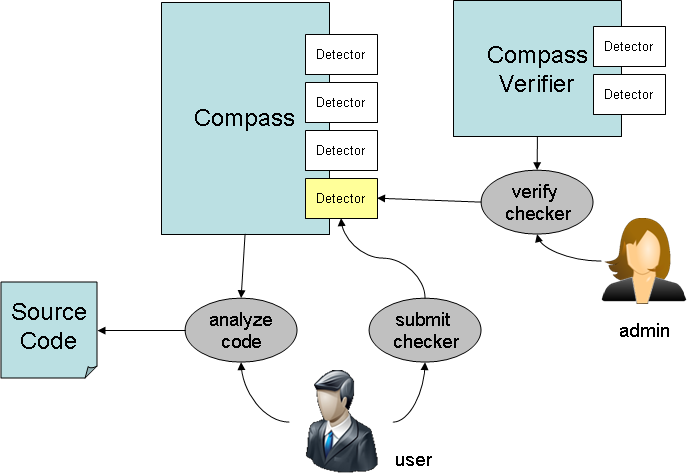
\includegraphics[width=4.5in]{compass_pic.png}
\caption{Compass Use Case}
\label{Compass_usecase}
\end{figure}

Furthermore, a user may contribute with his own detectors that he can add to Compass. Since 
external users may contribute detectors automatically via scripts, a verification of the 
validity and safety of these detectors is necessary. We provide a \emph{Compass Verifier}
that helps to check that all detectors are safe. Currently, the verifier is run by
a administrative person but may run automatically in the future.



\section{Design}

\begin{figure}[thb]
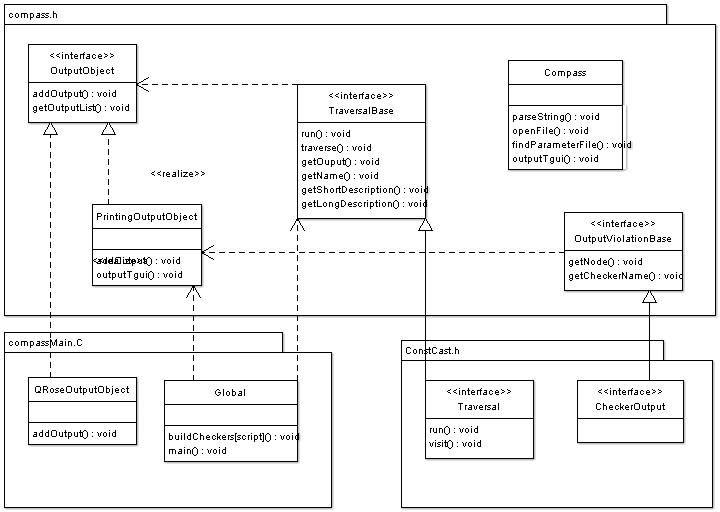
\includegraphics[width=6.0in]{compassdesign.png}
\caption{Compass Design}
\label{CompassDesign}
\end{figure}

Compass is designed to be easy to extend. Any user may write a detector and add it to Compass. Figure~\ref{CompassDesign}
illustrates the UML design decisions behind Compass.


Most of the functionality of Compass is in abstract classes hidden in the Compass namespace within compass.h - a file within
the compassSupport directory. All detectors, such as ConstCast illustrated in the figure, utilize the abstract classes
to traverse a program with all its nodes and to output violations found in that code according to the local algorithm.

CompassMain is the main executable that initially calls ROSE to parse a program. Then \emph{buildCheckers} is called to
load all detectors that are specified within a configuration file. The configuration file allows users to turn on and off
specific detectors for their run-time analyses. However, the configuration file only permits detectors to be loaded that 
were part of Compass at compile-time.

The main interface file compass.h contains the abstract classes \emph{TraversalBase} and 
\emph{OutputObject}. TraversalBase is the interface to ROSE, allowing a detector to traverse the ROSE AST (program) and hence
perform analysis on that AST. OutputObject aids to output defects found by a specific detector. More functionality to handle
e.g. file input and parameters provided to Compass, is provided within the Compass namespace.


\section{Compass Verifier}

\subsection{Threats} 

Compass must be safe, so that analyses and their results can be trusted. 
The main threats to the validity of Compass are:

\begin{itemize}
\item \emph{Malicious User}. A malicious user is an external user of Compass contributing a detector that performs malicious behaviour.  
\item \emph{Malicious Detector}. Compass is extensible and new detectos can be added externally (users outside the main development group).
  A detector can be programmed arbitrarily using the C/C++ and assembly programming languages. 
  It is therefore possible for a skilled programmer to hide malicious operations within a detector, e.g. allow a detector to scan the host machine and
  send data away. Compass must prevent detectors with malicious behaviour to be part of the Compass system. 
\item \emph{Source Code Replacement}. It should not be possible for users to exchange the source code of detectors within a running system,
  i.e. Compass cannot implement dynamic loading of detectors. Such a feature would compromise its safety.
\item \emph{Binary Replacement}. Another threat is the replacement of a valid Compass detector with a modified malicious version within a binary release of Compass.
  Therefore, Compass should be aware if parts of itself were modified and should not execute.
\end{itemize} 

\subsection{Safety Handling}

Compass is designed to be safe. The Compass Verifier is a stable separate copy of Compass that contains only a few detectors
to check (external and internal) user delivered detectors for safety. We have designed Compass in a way that it addresses the threats mentioned above:

\begin{itemize}
\item \emph{Malicious User}. Initially, we permit only trusted individuals to add new detectors to Compass. Once the verification process
  is matured, we will extend this policy to allow arbitrary users to contribute to Compass. 

\item \emph{Malicious Detector}. To prevent Compass to execute malicious code, the Compass Verifier executes its own detectors on
any user defined detector that is beeing considered to be added to Compass.
Currently, the Compass Verifier contains three detectors:

\begin{itemize}
\item \emph{fileReadOnlyAccess} ensures that a user defined detector perorms no write or execute operations on files. 
\item \emph{forbiddenFunctions} is a white list of function calls permitted in a detector. This list contains functions
that are trusted and hence considered unharmful when integrated to Compass.
\item \emph{noAsmStmtsOps} searches for assembly instructions in a detector and flags those as unsafe.
\end{itemize}

\item \emph{Source Code Replacement}. Detectors can only be added at compile time to Compass, not at run-time.
This means that detectors (meaning the source code) cannot be exchanged against unsafe versions at run-time. Furthermore, we allow only 
the Compass tool builder (admin) to build versions of Compass that must pass the Compass Verifier.

\item \emph{Binary Replacement}. Our goal is to perform a MD5 checksum on all the detectors part of the binary Compass distribution before
  Compass is executed. In this way Compass will not run if parts of it were modified.
\end{itemize} 


%The above list contains an important subset of detectors that enforce Compass detectors to be safe. 
%Additional detectors can easily be added to that list.
%In the future, a detector submitted to Compass, should go first through the automatic verifier, before it is either 
%added to Compass or denied.  




\chapter{Getting Started}

\label{gettingStarted:gettingStarted}

% \section{Building ROSE}

%  Purpose:
% \begin{itemize}
%    \item A. What you need to get started
%    \item B. Preparing the working copy
% \end{itemize}
% \begin{center}
% *********************  \newline
% \end{center}
% \vspace{0.25in}

   This chapter details how to build ROSE and how to begin to use ROSE to build a 
source-to-source translator.
ROSE uses EDG and SAGE III internally. EDG is a commercial (and proprietary) C++
frontend that we are permitted to use to support our research work. SAGE III is
loosely derived from SAGE II, which is derived from SAGE++.  SAGE III is a rewrite of 
SAGE II and uses a similar object-oriented design and a similar interface (API).
% We have made substantial changes in the development of Sage III, 
The developers of SAGE II suggested that we call our work on the C++
intermediate representation Sage III. We are thankful to the developers
of SAGE II for their work.
% It contains the software and hardware requirements of ROSE.
% Additionally, it details the installation of the software.

\section{ROSE Documentation and Where to Find It}

To simplify user access to the ROSE documentation, the pre-built postscript files are 
included in the {\tt ROSE/docs/Rose} directory of each ROSE distribution. These versions
are always kept up-to-date by the automated build system that generates
ROSE distributions:
% Documentation there is:
\begin{itemize}
   \item {\bf ROSE Web Page} : The ROSE Web page is located at
           \htmladdnormallink{www.roseCompiler.org}{http://www.roseCompiler.org}. \\
           The web page contains the ROSE manual, tutorial and developer API. 
           The API provides details about IR nodes and their usage (interfaces). The documentation
           is generated by Doxygen.
   \item {\bf ROSE offline Web content} : ROSE/docs/Rose/ROSE-\VersionNumber-HTML-Docs.ps.gz \\
       ROSE HTML documentation that is available without internet access.
   \item {\bf MANUAL} : ROSE/docs/Rose/ROSE-\VersionNumber-UserManual.ps.gz \\
       This is the ROSE User Manual which explains basic concepts about and capabilities within ROSE. \\
   \item {\bf TUTORIAL} : ROSE/docs/Rose/Tutorial/ROSE-\VersionNumber-Tutorial.tar.gz \\
       This is the ROSE Tutorial with numerous examples of how to use ROSE. \\
       The tutorial documentation is
           constructed using the following steps:
           \begin{enumerate}
              \item Actual source code for each example translator in the ROSE/tutorial
                    directory is included. 
              \item Each example is compiled.
              \item Inputs to the examples are taken from the ROSE/tutorial directory.
              \item Output generated from running each example is placed into the tutorial
                    documentation.
           \end{enumerate}
           Thus, the {\tt ROSE/tutorial} contains exact examples, and each
           example may be manipulated (changing either the example translators or the
           inputs to the examples).
   \item {\bf PAPERS} : ROSE/ROSE\_RESEARCH\_PAPERS.tar.gz \\
       These are the current ROSE related research papers.
\end{itemize}

\commentout{
   There are three forms of ROSE documentation, and a ROSE Web site and email list:
\begin{enumerate}
     \item ROSE User Manual \\
           The User Manual presents how to get started with ROSE and documents 
           features of the ROSE infrastructure.  The User Manual is found in 
           {\tt ROSE/docs/Rose} directory, or at the following web pages: \\
           \htmladdnormallink{ROSE User Manual (postscript version, relative link)}{http://www.rosecompiler.org/ROSE_UserManual/ROSE-0.9.5a-UserManual.ps}
           or \\
           \htmladdnormallink{ROSE User Manual (HTML version, relative link)}{http://www.rosecompiler.org/ROSE_UserManual/manual.html}
     \item ROSE Tutorial \\
           The ROSE Tutorial presents examples of how to use ROSE (found
           in the {\tt ROSE/tutorial} directory).  The ROSE Tutorial documentation is found in 
           {\tt ROSE/docs/Rose/Tutorial} directory and the tutorial documentation is
           constructed using the following steps:
           \begin{enumerate}
              \item Actual source code for each example translator in the ROSE/tutorial
                    directory is included. % into the tutorial documentation
              \item Each example is compiled.
              \item Inputs to the examples are taken from the ROSE/tutorial directory.
              \item Output generated from running each example is placed into the tutorial
                    documentation.
           \end{enumerate}
           Thus, the {\tt ROSE/tutorial} contains exact examples, and each
           example may be manipulated (changing either the example translators or the
           inputs to the examples).  The ROSE Tutorial can also be found at (link back 
           to LaTeX document): \\
           \htmladdnormallink{ROSE Tutorial (postscript version, relative link)}{http://www.rosecompiler.org/ROSE_Tutorial/ROSE-0.9.5a-Tutorial.ps}
           or \\
           \htmladdnormallink{ROSE Tutorial (html version, relative link)}{http://www.rosecompiler.org/ROSE_Tutorial/tutorial.html}
     \item ROSE HTML Reference: Intermediate Representation (IR) documentation \\
           This Web documentation gives the detail interfaces for each IR nodes
           (documentation generated by Doxygen).
           The HTML IR documentation is found in ROSE/docs/Rose directory 
           (available as HTML only): \\
           \htmladdnormallink{ROSE HTML Reference (relative
               link)}{http://www.rosecompiler.org/ROSE_HTML_Reference/index.html}
     \item ROSE Web Site \\
           The ROSE project maintains a Web site where this documentation and some
           additional information (including the ROSE software distribution:
           {\em starting late Summer 2006}) is available at
           \htmladdnormallink{ROSE Web Site
             (www.rosecompiler.org)}{http://www.rosecompiler.org}
     \item ROSE Email List \\
           The ROSE project maintains a mailing list (rose-public *at* nersc *dot* gov).
           Anyone who would like to be on the email list can subscribe to
           it at:
           \htmladdnormallink{ROSE Public Email List}
                {https://mailman.nersc.gov/mailman/listinfo/rose-public}.
\end{enumerate}
}

% DQ (1/20/2009): Fixing the reference to the email list for ROSE.
The ROSE project maintains an external mailing list (see information at:
\htmladdnormallink{www.roseCompiler.org}{http://www.roseCompiler.org} and click on the
{\bf Mailing Lists} link for how to join).

\section{ROSE Installation}

\subsection{Requirements and Options}
\label{Requirements_Installation_Testing}
   ROSE is general software and we ultimately hope to remove any specific software
and hardware requirements.  However, our goal is to be specific about where and 
how ROSE is developed and where it is regularly tested.
% ROSE has been developed initially on the Sun workstations and later on Linux.
% Since ROSE is written in C++, it requires a C++ compiler. Some optional features
% within ROSE have some additional software requirements.

\subsubsection{Required Hardware/Operating System}
   ROSE has been developed on Linux/Intel platforms. We have not yet 
addressed significant portability issues for ROSE. But EDG has addressed
portability issues for their C++ frontend and it is available on nearly all
platforms (see {\tt www.EDG.com} for details).  ROSE is currently developed on
Linux/Intel platforms and works with all modern versions of the GNU compilers 
(3.4.x, and later). ROSE also works on both 32-bit and 64-bit architectures, 
as well as with the Intel C and C++ compilers.  Recent work has ported ROSE
to both Mac OSX and Cygwin (under Microsoft Windows).

Future work will focus on portability to other platforms important to users.
If you have a specific requirement for ROSE to be ported to a target platform
please let us know.
% At a later point we will address portability of ROSE onto other platforms:
% mostly likely IBM AIX will be next (at some point).

\subsubsection{Software Requirements}
   You will require {\bf ONLY} a C++ compiler to compile ROSE; ROSE is written in C++.
% We use the GNU g++ compiler most often, but the Intel compiler (version 9.1) will also work.
Present development work is done on Intel/Linux platforms
%using the GNU g++ 3.3.x, 3.4.x, and 4.x; and the Intel compilers.  GNU compilers older
using the GNU g++ 3.4.x, and 4.x; and the Intel compilers.  
%GNU compilers older
%than 3.3.x are not supported within the ROSE project, but in some cases they might work 
%(g++ 3.2.x is likely to work, but g++ 2.96 will not work).

   ROSE users may either obtain a free research license from EDG and hence ROSE with EDG source code,
or alternatively, obtain ROSE that contains a binary version of the EDG work.
The latter is limited to specific platforms and versions of compilers. See EDG (www.edg.com) for details 
and limitations on how their software may be used. There is more information in the 
ROSE Manual (see chapter {\em Getting Started}
section {\em Getting a Version of the EDG License for Research Use}).

\commentout{
   We suggest that ROSE users obtain a free research license from EDG until we 
regularly distribute binary versions of the libedg.so library (their software).
Email us for details on our distributions of ROSE that contain a binary version
of the EDG work (and that completely hide the EDG interface). These are limited
to specific platforms and versions of compilers. See EDG (www.edg.com) for details 
and limitations on how their software may be used.
}

{\bf Required Software:} \\
  The following software is required in order to build and use ROSE 
(see note about Mac OSX as well):
\begin{itemize}
   \item {\bf ROSE}: \\
     There are three versions of ROSE supported: the {\it Distribution Version} for users
    (typical), the {\it External Development Version} for advanced users and collaborators, 
     and the {\it Internal Development Version} (intended only for ROSE development team
     and external developers with access to our internal SVN repository which includes the
     EDG source code). The development versions are what are found in the ROSE software
     repositories and have additional software requirements (subversion, JDK, autoconf,
     automake, Doxygen, LaTeX, etc.).
   % The exact requirements are listed in the {\tt ROSE/ChangeLog} (including version numbers for each release of ROSE).
     \begin{itemize}
       \item {\bf Distribution Version} \\
       Provided as a tared and compressed file in the form, ROSE-\VersionNumber.tar.gz.
       It can be obtained from \htmladdnormallink{outreach.scidac.gov/projects/rose}{https://outreach.scidac.gov/projects/rose/}. 
       This is the most typical way that users will see and work with ROSE. But it is less
       up-to-date compared to development versions.

       \item {\bf External Development Version } \\
       It is available from the SciDAC Outreach Center's subversion repository:
       \htmladdnormallink{outreach.scidac.gov/projects/rose}{https://outreach.scidac.gov/projects/rose/}.
       We put a subset (excluding the EDG part essentially) of the internal developer version of
       ROSE into the external repository to enable people to have quick access to the most
       recent new features in ROSE.  The external repository is synchronized with the
       internal repository once a day in ideal conditions. Several branches also exist to
       accept contributions from external collaborators.

       \item {\bf Internal Development Version} \\
       Only available directly from the LLNL's internal Subversion (SVN) repository. 
       The details of building this version are located in the Appendix of the Manual. %\ref{gettingStarted:DeveloperInstructions}.
     \end{itemize}
    % ROSE is delivered as either a development version (svn) or as a distribution for
    % users. The (typical) user version comes either with EDG source or binary distribution.

   \item {\bf g++} : version $>=$ 3.4.x  \\
     In order to use OpenMP or gFortran g++ $>=$ 4.2.x is required.

   \item {\bf BOOST} : version $>=$ 1.35.0  \\
     Visit \htmladdnormallink{www.boost.org}{http://www.boost.org/}
     for more details about BOOST and \htmladdnormallink{www.boost.org/users/download}{http://www.boost.org/users/download/}
     for download and installation instructions. 
     {\em Installation of Boost is such a common issue that we include simple directions for how to install Boost in section~\ref{gettingStarted:BOOST}}

   \item {\bf JAVA} : version $>$1.5.0\_11 \\
     A SUN Java virtual machine (JVM) is needed. A Java compiler (JDK) is also
     required for development versions.  

   \item {\bf Autoconf} : version $>=$ 2.59. Needed \emph{ONLY} for development versions. \\
     Autoconf is an extensible package of M4 macros that produce shell scripts to automatically configure software source code packages. 

   \item {\bf Automake} : version $>=$ 1.96. Needed \emph{ONLY} for development versions. \\
     Automake is a tool for automatically generating `Makefile.in' files compliant with
     the GNU Coding Standards.

   \item {\bf Libtool}: version $>=$1.5.6.  Needed \emph{ONLY} for development versions. 
\end{itemize}

\paragraph{Mac OSX Support:}
   It has been reported that our binary version of EDG requires Mac OS 10.5
(which might make sense because we build it using Mac OSX version 10.5.6).  More
specifically there are unresolved references during linking ROSE applications with
Mac OS from 10.4.11; the solution is to upgrade your Mac OS.  Note that Mac OSX 
version 10.4 is fairly old and so this should not be a problem on more modern Apple
systems.  Our report about this fix also says that upgrading Xcode from version 2.4 
to version 3.3, might be related.

Note that on our Mac OSX (version 10.5.6), all of our testing of ROSE uses the following packages:
\begin{itemize}
   \item {\bf boost\_1\_35\_0.tar.gz}:
     All installations of ROSE (any platform) require boost.

   \item {\bf doxygen-1.5.6.src.tar.gz}:
     Doxegen is required to build the documentation which is both distributed with ROSE
     and make available via the ROSE web site.

   \item {\bf ghostscript-8.62.tar.gz}:
     Not clear that this is really required by ROSE.

   \item {\bf latex2html-2002-2-1.tar.gz}:
     Likely required by LaTeX (not required by ROSE as far as I know).

   \item {\bf texlive2007-live-20070212.iso.zip (LaTeX)}:
     Reqired to build the latex documentation (ROSE Manual and ROSE Tutorial).

   \item {\bf fontconfig-2.6.0.tar.gz}:
     Not clear that this is really required by ROSE.

   \item {\bf graphviz-2.20.1.tar.gz}:
     Required to generate graphs for the LaTex documentation in ROSE.

   \item {\bf libtool-2.2.4.tar.bz2}:
     Required to build ROSE (used in ROSE configuration management).
\end{itemize}

As an extra detail, our .bashrc file for Mac OSX is:
\begin{verbatim}
export DYLD_LIBRARY_PATH="/Users/dquinlan/local/boost_1_35_0_installTree-gxx-4.0.1/lib"
export PATH="/Users/dquinlan/local/doxygen-install/bin:$PATH"
export PATH="/Users/dquinlan/local/graphviz-install/bin:$PATH"
export PATH="/Users/dquinlan/local/texlive-install/2007/bin/i386-darwin/:$PATH"
export PATH="/Users/dquinlan/local/latex2html-install/bin/:$PATH"
export PATH="/Users/dquinlan/local/ghostscript-install/bin/:$PATH"
export PATH="/Users/dquinlan/local/fontconfig-install/bin/:$PATH"
\end{verbatim}

   We are not significant Mac users, ROSE is primarily developed under Linux, 
however we are particularly interested in supporting collaborators who are, 
so Mac OSX support is important to us.  We would appriciate any help in making 
sure that ROSE installs smoothly on both Mac OSX and Linux.



To simplify the descriptions of the build process, we define:
\begin{itemize} 
   \item {\bf Source Tree} \\
         Location of source code directory (there is only one source tree).
   \item {\bf Compile Tree} \\
         Location of compiled object code and executables. There can be many compile trees
         representing either different: configure options, compilers used to build ROSE
         and ROSE translators, compilers specified as backends for ROSE (to compile ROSE
         generated code), or architectures.
\end{itemize}

We {\em strongly} recommend that the {\bf Source Tree} and the {\bf Compile Tree} be
different. This avoids many potential problems with the {\em make clean} rules.
Note that the {\bf Compile Tree} will be the same as the {\bf Source Tree}
if the user has {\em not} explicitly generated a separate directory in which to
run {\em configure} and compile ROSE. If the {\bf Source Tree} and {\bf Compile Tree} 
are the same, then there is only one combined {\bf Source/Compile Tree}.
Alternatively, numerous different {\bf Compile Trees} can be used from 
a single {\bf Source Tree}.  More than one {\bf Compile Tree} allows
ROSE to be generated on different platforms from a single source 
(either a generated distribution or checked out from SVN).  ROSE is developed 
and tested internally using separate {\bf Compile Trees}. \\


{\bf Use of Optional Software:} \\
%ROSE does not presently require any special software, but more
More functionality within ROSE is available if one has additional (freely available) software installed:
\begin{itemize}
   \item {\bf libxml2-devel }: \\
         Several optional features of ROSE need to handle XML files, such as
         roseHPCT and BinaryContextLookup.
   \item {\bf Doxygen} : \\
          Most ROSE documentation is generated using LaTex and Doxygen, thus
          Doxygen is required for ROSE developers that want to regenerate the ROSE
          documentation. This is not required for ROSE users, since all documentation is 
          included in the ROSE distribution. Visit {\it www.doxygen.org} for details and to
          download software.  There are no ROSE-specific configure options to use Doxygen;
          it must only be available within your path.
   \item {\bf LaTeX} : \\
          LaTeX is used for a significant portion of the ROSE documentation. LaTex is 
          included on most Unix systems. There are no ROSE specific configure options 
          to use LaTeX; it must only be available within your path.
   \item {\bf DOT (GraphViz)} : \\
          ROSE uses DOT for generating graphs of ASTs, Control Flow, etc.
          DOT is also used internally by Doxygen.
          Visit {\it www.graphviz.org} for details and to download software.
          An example showing the use of the DOT to build graphs is in the ROSE Tutorial.
          There are no ROSE-specific configure options to use dot; it must only be 
          available within your path.
   \item {\bf SQLite} : \\
          ROSE users can store persistent data across separate compilation of files by
          storing information in an SQLite database.  This is used by several features
          in ROSE (call-graph generation, for example) and may be used directly by the
          user for storage of user-defined analysis data.  Such database support is
          one way to handle global analysis (the other way is to build the whole
          application AST). Visit {\it www.sqlite.com} for details and to download
          software. %Details are in section \ref{gettingStarted:Database}.
          An example showing the use of the ROSE database mechanism is in the ROSE
          Tutorial. Use of SQLite requires special ROSE configuration options (so that
          the SQLite library can be added to the link line at compile time).  See ROSE
          configuration options for more details ({\tt configure --help}).
   \item {\bf mpicc} : \\
          mpicc is a compiler for MPI development. If ROSE is configures with MPI
          enabled, one can utilize features in ROSE that allow for distributed
          parallel AST traversals.
\end{itemize}

% \subsection{Installation and Testing }

%\subsection{How to Build ROSE}

\commentout{
%   This section addresses the building and installation of ROSE.  
There are two versions of ROSE supported: the 
{\it Distribution Version} for users (typical) and the {\it Development Version}
(intended only for ROSE development team), which is what is found in the ROSE software
repository and has additional software requirements (autoconf, automake, Doxygen, LaTeX,
etc.).  The exact requirements are listed in the {\tt ROSE/ChangeLog} (including version 
numbers for each release of ROSE).
\begin{itemize}
   \item {\bf Distribution Version} \\
         Provided as a tared and compressed file in the form,
         ROSE-\VersionNumber.tar.gz.  This is the most typical way that users will
         see and work with ROSE.  Instructions are also located in the ROSE/README file.

   \item {\bf Development Version} \\
         Only available directly from the Subversion (SVN) repository. The details of building this
         version are located in the Appendix \ref{gettingStarted:DeveloperInstructions}.
\end{itemize}  
To simplify the descriptions of the build process, we define:
\begin{itemize} 
   \item {\bf Source Tree} \\
         Location of source code directory (there is only one source tree).
   \item {\bf Compile Tree} \\
         Location of compiled object code and executables. There can be many compile trees
         representing either different: configure options, compilers used to build ROSE
         and ROSE translators, compilers specified as backends for ROSE (to compile ROSE
         generated code), or architectures.
   \item {\bf Install Tree} \\
         Location of compiled object code when copied to a clean installation directory.
         This is commonly used in order to refer to a project from outside, i.e. to 
         use the provided interfaces. 
\end{itemize}

We {\em strongly} recommend that the {\bf Source Tree} and the {\bf Compile Tree} be
different. This avoids many potential problems with the {\em make clean} rules.
Note that the {\bf Compile Tree} will be the same as the {\bf Source Tree}
if the user has {\em not} explicitly generated a separate directory in which to
run {\em configure} and compile ROSE. If the {\bf Source Tree} and {\bf Compile Tree} 
are the same, then there is only one combined {\bf Source/Compile Tree}.
Alternatively, numerous different {\bf Compile Trees} can be used from 
a single {\bf Source Tree}.  More than one {\bf Compile Tree} allows
ROSE to be generated on different platforms from a single source 
(either a generated distribution or checked out from SVN).  ROSE is developed 
and tested internally using separate {\bf Compile Trees}.
}

\commentout{
\subsection{Summary of Build Process}
\label{gettingStarted:SummaryInstructions}
   More specific information is available in the subsections below 
(subsection \ref{gettingStarted:UserInstructions} and 
subsection \ref{gettingStarted:DeveloperInstructions}), but in summary the steps are:
% The general steps are (but use the more details instructions below, depending 
% on the version of ROSE that you have):
\begin{itemize}
   \item Type {\tt \<Source Tree\>/configure;} \\
         This can be done in a separate directory or in the source directory.
         We suggest using a separate directory, but either will work. The 
         {\bf Source Tree} may be specified with either an absolute or relative 
         path.
   \item type {\tt make} \\ to build the source code (you may also use the parallel make
         option (e.g. {\tt make -j4} to run make using 4 processes).
   \item Type {\tt make check} \\ to run internal tests to test your build.
   \item Type {\tt make install} \\ to install the build library for more convenient use.
         (default is {\tt /usr/local}, use {\tt --prefix=`pwd'} to specify the current directory).
   \item Type {\tt make documentation} \\ to build both html and LaTeX documentation.
\end{itemize}
}

\subsection{Building BOOST}
\label{gettingStarted:BOOST}

The following is a quick guide on how to install BOOST. For more details please 
refer to \htmladdnormallink{www.boost.org}{http://www.boost.org/}:

\begin{enumerate}
     \item Download BOOST. \\
       Download BOOST at \htmladdnormallink{www.boost.org/users/download}{http://www.boost.org/users/download/}.
     \item Untar BOOST. \\
       Type {\tt tar -zxf BOOST-[VersionNumber].tar.gz} to untar the BOOST distribution.
% DQ (10/20/2008): Removed as suggested by Andy stone, separate compile tree for boost is
%                  more complex than required and can exhibit a bug in Boost.
%     \item Create a separate compile tree. \\
%           Type {\tt mkdir compileTree} to build a location for the object files and
%           documentation (use any name you like for this directory, e.g. BOOST\_BUILD).
     \item Create a separate install tree. \\
           Type {\tt mkdir installTree} to create a location for the install filesto reside (e.g. BOOST\_INSTALL).
% DQ (10/20/2008): Removed as suggested by Andy stone, separate compile tree for boost is
%                  more complex than required and can exhibit a bug in Boost.
%     \item Change directory to the new compile tree directory. \\
%           Type {\tt cd compileTree; }. This changes the current directory to the newly
%           created directory.
     \item Run the {\tt configure} script. \\
%          Type {\tt \{AbsoluteOrRelativePathToSourceTree\}/configure --prefix=[installTree]} 
           Type {\tt ./configure --prefix=[installTree]} 
           to run the BOOST {\tt configure} script.  The path to the configure script 
           may be either relative or absolute. The prefix option specifies the installation directory (e.g. BOOST\_INSTALL).
     \item Run {\tt make}. \\
           Type {\tt make} to build all the source files. 
     \item Run {\tt make install}. \\
           Type {\tt make install} to copy all build files into the install directory. BOOST is now available in your 
           installTree (e.g. BOOST\_INSTALL) to be used by ROSE.
\end{enumerate}

% DQ (7/19/2008): Added the subject which stopped at least one user from LSU.
  Note that the installation of Boost will frequently output 
warnings (e.g. {\em *(Unicode/ICU support for boost.regex?..not found).*},
these can be ignored.

\subsection{Building ROSE From a Distribution (ROSE-\VersionNumber.tar.gz)}
\label{gettingStarted:UserInstructions}
   The process for building ROSE from a ROSE {\em Distribution Version} is the same as for
    most standard software distributions (e.g those using autoconf tools):
\begin{enumerate}
     \item Untar ROSE. \\
           Type {\tt tar -zxf ROSE-\VersionNumber.tar.gz} to untar the ROSE distribution.
     \item Build a separate compile tree. \\
           Type {\tt mkdir compileTree} to build a location for the object files and
           documentation (use any name you like for this directory).
     \item Change directory to the new compile tree directory. \\
           Type {\tt cd compileTree; }. This changes the current directory to the newly
           created directory.
     \item Add JAVA environment variables. \\
           For example:\\
           {\tt export JAVA\_HOME=/usr/apps/java/jdk1.5.0\_11} \\
        {\tt export
        LD\_LIBRARY\_PATH=\$JAVA\_HOME/jre/lib/i386/server:\$LD\_LIBRARY\_PATH}

     \item Add the Boost library path into your LD\_LIBRARY\_PATH.\\
           For example: {\tt
           LD\_LIBRARY\_PATH=\$LD\_LIBRARY\_PATH:/home/youraccount/opt/boost\_1\_35\_0/lib}
     \item Run the {\tt configure} script. \\
           Type {\tt \{AbsoluteOrRelativePath\}/configure --prefix=`pwd` --with-boost=[BOOST\_installTree]} 
           to run the ROSE {\tt configure} script.  The path to the configure script 
           may be either relative or absolute. The prefix option on the configure 
           command line is only required if you run {\tt make install} (suggested), because 
           the default location for installation is {\tt \//usr\//local} and most users don't
           have permission to write to that directory. This is common to all projects that
           use autoconf.  ROSE follows the GNU Makefile Standards as a result of using
           autoconf and automake tools for its build system. As of ROSE-0.8.9a, the
           default setting for the install directory (prefix) is the build tree.
           For more on ROSE configure options, see section \ref{gettingStarted:configureOptions}.
     \item Run {\tt make}. \\
           Type {\tt make} to build all the source files. See details of running 
           {\tt make} in parallel in section \ref{gettingStarted:parallelMake}.
     \item To test ROSE (optional). \\
           Type {\tt make check} to test the ROSE library against a collection of test codes.
           See details of running make in parallel \ref{gettingStarted:parallelMake}.
     \item To install ROSE, type {\tt make install}. \\
           Installation is optional, but suggested. Users can simplify their use of ROSE 
           by using it from an installed version of ROSE.  This permits compilation 
           using a single include directory and the specification of only two libraries.
           See details of installing ROSE in section \ref{gettingStarted:installation}.
     \item Testing the installation of ROSE (optional). \\
           To test the installation and the location where ROSE is installed, against a
           collection of test codes (the application examples in {\tt ROSE/tutorial}), 
           type {\tt make installcheck}.
           A sample {\tt makefile} is generated.%; see section \ref{gettingStarted:compilingTranslator}.
\end{enumerate}
\subsection{Building ROSE from a Development Version}
Building ROSE from an internal or external development version is very
similar to building it from a distribution. The major difference is that
for development versions, you have to type ./build in the source tree to 
generate the configure script and Makefile.ins. Once this is done, the rest
steps are the same as those of building a distribution version.

\subsection{TroubleShooting the ROSE Installation}

% DQ (11/12/2008): This is where we need to accumulate the symptoms of what goes wrong.

   There are a number of famous ways to screw up yur installation of ROSE.
\begin{enumerate}
   \item Message: {\tt configure: error: Could not link against boost\_filesystem-gcc41-mt} \\
   This message from running the {\tt configure} command in ROSE (an initial step in building
   ROSE) indicates that your {\tt LD\_LIBRARY\_PATH} (environment variable) is not set to 
   to the location of the boost install tree.  The ROSE configure scripts (autoconf) will
   test the linking to specific boost libraries and this is the first dynamic link library 
   that it tests and so it will fail when many other tests on boost succeed because your
   {\tt LD\_LIBRARY\_PATH} is finally required and is not properly set.

 % Note from Matt (11/23/2008): Fixed it -- I just gave up one the libtool that came with
 % the apple dev tools and just built my own libtool in my home directory.  All is
 % compiling fine now.
   \item Message: {\tt Making all in libltdl \\
      make[2]: *** No rule to make target `all'.  Stop.} \\
   Run {\tt glibtoolize --force} to rebuild the libtool support in ROSE for your machine 
   at the top level of the source tree. If that does not work then give up on the libtool 
   that came with the apple dev tools and just build your own libtool in your home directory.

   \item {\bf Don't build ROSE in the source tree, it is not tested often, but it should work.} \\
    Save yourself some trouble and build a separate compile tree.  This will also allow
    you to build a number of different versions of ROSE with different options.

    \item Message: {\bf configure: error: Unable to find path to JVM library} \\
   This message from running the {\tt configure} command in ROSE (an initial step in building
   ROSE) indicates either that your {\tt LD\_LIBRARY\_PATH} (environment variable) is not set to 
   to the location of the {\em libjvm.so} or that your machines java is not one that we
   support (e.g. non-Sun Java).  If you don't require Java (e.g. don't need Fortran
   support) then consider skipping the java support by using {\em --without-java} on the
   configure command line.
   Alternatively, your {\tt LD\_LIBRARY\_PATH} should contain the path to the file 
   {\em libjvm.so}.  The likely path is specified in the lines just before the message.  
   The full message will appear as:
\begin{verbatim}
checking for Java... /usr/lib/jvm/java-1.5.0-ibm.x86_64/bin/../bin/java
checking for Java JVM include and link options... JavaJREDir  = /usr/lib/jvm/java-1.5.0-ibm-1.5.0.8.x86_64/jre/bin
JavaHomeDir = /usr/lib/jvm/java-1.5.0-ibm-1.5.0.8.x86_64
JavaJVMDir  = /usr/lib/jvm/java-1.5.0-ibm-1.5.0.8.x86_64/jre/bin/classic
configure: error: Unable to find path to JVM library
\end{verbatim}

   \item Previously installed version of Boost library. \\
    Some machines have a default version of Boost already installed (for example in 
{\tt /usr/include/boost}).  This always the wrong version since the OS installation
of Boost lags by several years.  ROSE now attempts to detect this and use the 
\quote{-isystem} g++ option to have the explicitly specified version of boost from
the configure command-line be search before the system include directories.  This works
well where a machine has a previously installed version of Boost, but it will fail when
used with SWIG (so don't use {\tt --with-javaport} where a previous system installation
of Boost is detected).  The ROSE configure scripts will detect the presence of a
previously installed version of Boost and issue a warning message to not use 
{\tt --with-javaport}.  Also if no previously installed version of Boost is detected
the configuration will report this as well and make clear that it will use the Boost
include directory with a {\tt -I} option.

   \item libtoolize not available (or old version) \\
  The problem is that ROSE is calling {\tt libtoolize} or {\tt glibtoolize} and 
it seems that you don't have it on your machine (called by the build script). 
You will need it, it is a requirement. The {\tt build} script will run this to build you the
required libtool support.  Since this happens upsteam of {\tt configure} we don't have a test
for it. The clue is the output:
\begin{verbatim}
ls: cannot access libltdl/*: No such file or directory
libtoolize: cannot list files in `/usr/share/libtool/libltdl'
\end{verbatim}
If you build libtool on your machine and add the installed libtool {\tt bin} directory
to you path, then it should work.  I often use {\tt libtool-2.2.4.tar} when I have 
this problem on a new platform.

Report from use:
\begin{verbatim}
Reason for the problem: I am not building libtools from source, instead using
the packages from the Linux distribution repository. On my distribution
(Ubuntu 8.04, X86_64), the libltdl3 (and libltdl3-dev)  does not come with
the libtool package. After installing the libtools, I still need to install
both the libltdl3 and libltdl3-dev package. That is the issues of unable to
find libltdl folders.
\end{verbatim}


\end{enumerate}



\subsection{ROSE Configure Options}
\label{gettingStarted:configureOptions}
     A few example configure options are:
\begin{itemize}
   \item Minimal configuration \\
         {\tt ../ROSE/configure --with-boost=[BOOST\_installTree]} \\
         This will configure ROSE to be compiled in the current directory (separate from
         the {\bf Source Tree}).  The installation (from {\tt make install}) will be placed in
         {\tt /usr/local}.  Most users don't have permission to write to this directory,
         so we suggest always including the {\em prefix option} (e.g. {\tt
         --prefix=`pwd`}).
   \item Minimal configuration (prefered) \\
         {\tt ../ROSE/configure --prefix=`pwd` --with-boost=[BOOST\_installTree]} \\
         Configure in the current directory so that installation will also happen in the
         current  directory (a {\tt install} subdirectory will be built).
   \item Turning on compiler debugging options (prefered) \\
         {\tt ../ROSE/configure --with-CXX\_DEBUG=-g --with-C\_DEBUG=-g 
              --with-CXX\_WARNINGS=-Wall --prefix=`pwd`--with-boost=[BOOST\_installTree]} \\
         Configure as above, but with debugging and warnings turned on ({\tt -Wall} is
         specific to the gnu compilers).
   \item Adding Fortran support \\
         {\tt ../ROSE/configure --prefix=`pwd` --with-boost=[BOOST\_installTree] --with-java} \\
         The Open Fortran Parser will also be enabled, allowing ROSE to process Fortran
         code.  The programs {\tt java}, {\tt javac}, and {\tt jar} must be either in your 
         PATH or in {\tt \$JAVA\_HOME/bin}.
   \item Adding SQLite support \\
         {\tt ../ROSE/configure --with-sqlite3=/home/dquinlan/SQLite/sqliteCompileTree --prefix=`pwd` --with-boost=[BOOST\_installTree]} \\
         Configure as above, but permit use of SQLite database for storage of analysis
         results between compilation of separate files (one type of support in ROSE for
         global analysis).
   \item Adding parallel distributed memory analysis support (using MPI) \\
         {\tt ../ROSE/configure --prefix=`pwd` --with-mpi --with-gcc-omp --with-boost=[BOOST\_installTree]} \\
         Configure as above, but with MPI and OpenMP support for ROSE to run AST traversals
         in parallel (distributed and shared memory).
   \item Adding IDA Pro support \\
         {\tt ../ROSE/configure --prefix=`pwd` --with-binarysql --with-boost=[BOOST\_installTree]} \\
         The binarysql flag allows ROSE to read a binary file previously stored as a sql file (e.g. fetched from
         IDA Pro). 
   \item Adding support for SWIG (Python connection) \\
         {\tt ../ROSE/configure --prefix=`pwd` --with-javaport=yes SWIG=swig --with-boost=[BOOST\_installTree] --with-java} \\
         This allows ROSE to be build with javaport, a support that connects ROSE to Java via SWIG.
         The Eclipse plug-in to ROSE is based on this work.
   \item Additional Examples \\ 
         More detailed documentation on configure options can be found by typing 
         {\tt configure --help}, or see figure
         \ref{gettingStarted:configureHelpOptionOutputPart1} for complete
         listing.
\end{itemize}



%\fixme{It is suggested by TID that we move the figures to this location.
%       Checkout if this is possible.}

Output of {\tt configure --help} is detailed in Figures 
\ref{gettingStarted:configureHelpOptionOutputPart1} (Part 1) and
\ref{gettingStarted:configureHelpOptionOutputPart2} (Part 2):
{\indent
{\mySmallestFontSize
% Do this when processing latex to generate non-html (not using latex2html)
\begin{latexonly}
\begin{figure}[tb]
\begin{center}
\begin{tabular}{|c|} \hline
     {\tt configure --help} Option Output (Part 1)
\\\hline\hline
{\tiny
   \lstinputlisting{roseConfigureOptions.aa}
}
\\\hline
\end{tabular}
\end{center}
\caption{ Example output from configure --help in {\tt ROSE} directory (Part 1). }
\end{figure}
\end{latexonly}

% Do this when processing latex to build html (using latex2html)
\begin{htmlonly}
   \verbatiminput{roseConfigureOptions.aa}
   \vspace{0.5in}
   Example output from configure --help in {\tt ROSE} directory (Part 1).
\end{htmlonly}
\label{gettingStarted:configureHelpOptionOutputPart1}
%end of scope in font size
}
% End of scope in indentation
}

% Output of {\tt configure --help} (Part 2):
{\indent
{\mySmallestFontSize
% Do this when processing latex to generate non-html (not using latex2html)
\begin{latexonly}
\begin{figure}[tb]
\begin{center}
\begin{tabular}{|c|} \hline
     {\tt configure --help} Option Output (Part 2)
\\\hline\hline
{\tiny
   \lstinputlisting{roseConfigureOptions.ab}
}
\\\hline
\end{tabular}
\end{center}
\caption{ Example output from configure --help in {\tt ROSE} directory (Part 2). }
\end{figure}
\end{latexonly}

% Do this when processing latex to build html (using latex2html)
\begin{htmlonly}
   \verbatiminput{roseConfigureOptions.ab}
   \vspace{0.5in}
   Example output from configure --help in {\tt ROSE} directory (Part 2).
\end{htmlonly}
\label{gettingStarted:configureHelpOptionOutputPart2}
%end of scope in font size
}
% End of scope in indentation
}


\subsection{Running {\em GNU Make} in Parallel}
\label{gettingStarted:parallelMake}
     ROSE uses general {\tt Makefiles} and is not dependent on {\em GNU Make}.
     However, {\em GNU Make} has an option to permit compilation in parallel and 
     we support this. Thus you may use {\tt make} with the {\tt -j<n>} option if 
     you want to run {\tt make} in parallel (a good value for {\tt n} is typically 
     twice the number of processors in your computer).  We have paid special 
     attention to the design of the ROSE {\em makefiles} to permit parallel 
     {\tt make} to work; we also use it regularly within development work.

\subsection{Installing ROSE}
\label{gettingStarted:installation}
     Installation (using {\tt make install}) is optional, but suggested. Users can
simplify their use of ROSE by using it from an installed version of ROSE.  This permits
compilation using a single include directory and the specification of only two libraries, 
as in:
\begin{verbatim}
     g++ -I{\<install dir\>/include} -o executable executable.C 
         -L{\<install dir\>/lib} -lrose -ledg -lm $(RT_LIBS)
\end{verbatim}
% $ reset emacs highlighting

See the example makefile in \\
{\tt ROSE/exampleTranslators/documentedExamples/simpleTranslatorExamples/exampleMakefile} \\
in Section \ref{gettingStarted:compilingTranslator}
for exact details of building a translator on your machine (setup by configure and tested
by {\tt make installcheck}).  Note that the tutorial example codes are also tested
by {\tt make installcheck} and the {\tt example\_makefile} there can also serve as
an example.

     {\bf autoconf} uses {\tt /usr/local} as the default location for all 
installations. Only {\em root} has write privileges to that directory, so you
will likely get an error if you have not overridden the default value with a new
location.  To change the location, you need to have used the 
{\tt --prefix=\{install\_dir\}} to run the {\tt configure} script.  You can 
rerun the {\tt configure} script without rebuilding ROSE.

%\fixme{ROSE-0.8.9a now sets the default install path (prefix) to the build tree. The
%    documentation does not yet really reflect this detail.  Also since the build process
%    writes to the install directory we have to explain this in the documentation.}

\subsection{MPI Support}
     ROSE supports the use of MPI for parallel distributed memory program analysis, a
research focus within the ROSE project.  To support this use the {\tt --with-mpi}
option on the configure command line.  If you get the following message:
%{\footnotesize
\begin{verbatim}
configuration file /home/<user name>/.mpd.conf not found
A file named .mpd.conf file must be present in the user's home
directory (/etc/mpd.conf if root) with read and write access
only for the user, and must contain at least a line with:
MPD_SECRETWORD=<secretword>
One way to safely create this file is to do the following:
  cd $HOME
  touch .mpd.conf
  chmod 600 .mpd.conf
and then use an editor to insert a line like
  MPD_SECRETWORD=mr45-j9z
into the file.  (Of course use some other secret word than mr45-j9z.)
\end{verbatim}
%}
% $ reset emacs highlighting
Then follow the directions to build the {\tt .mpd.conf} file.  The use of the 
MPI configure option will allow additional code in ROSE to be compiled and 
additional tests to be run.


\subsection{Testing ROSE}
     A set of test programs is available.  %More details are in section \ref{testing}.
% written about this in later versions of the manual.  
Type {\tt make check} to run your build version of ROSE using these test codes.  
Several years of contributed bug reports and internal test codes have been accumulated 
in the {\tt ROSE/tests} directory.

Extra tests are available for development versions of ROSE. ROSE developers
are highly recommended to run {\tt make dist} and {\tt make distcheck} to make
sure that the modified development versions can be used to create functioning
distributions.

\subsection{Getting Help}
%     You may use the following mailing list to ask for help from the ROSE development 
% team: {\it casc-rose *dot* llnl *dot* gov}.
%    The ROSE project maintain a number of email lists for internal development, 
% external devlopers, and external users. More information is in the ROSE User Manual
% in the Developer's Appendix (see \ref{rose_email_list_info}).

% DQ (1/21/2009): Note this information is maintained in several locations and in LaTeX
% and doxygen formats:
%    1) ROSE User Manual: Developer's: Appendix,
%    2) ROSE Installation Manual
%    3) ROSE Tutorial
%    4) doxygen generated web pages for ROSE (rose.docs.in and AvailableDocumentation.docs.in)
%
% DQ (10/28/2008): This information is copied from:
%                  ROSE User Manual: Developer's: Appendix: ROSE Email Lists.

We have three mailing lists for core developers (those who have write access to
the internal repository), all developers (anyone who has write access to the
internal or external repository) and all
users of ROSE. They are:
\begin{itemize}
\item rose-core@nersc.gov, web interface: 
\htmladdnormallink{https://mailman.nersc.gov/mailman/listinfo/rose-core}{https://mailman.nersc.gov/mailman/listinfo/rose-core}.
\item rose-developer@nersc.gov, web interface: 
\htmladdnormallink{https://mailman.nersc.gov/mailman/listinfo/rose-developer}{https://mailman.nersc.gov/mailman/listinfo/rose-developer}.
\item rose-public@nersc.gov, web interface:
\htmladdnormallink{https://mailman.nersc.gov/mailman/listinfo/rose-public}{https://mailman.nersc.gov/mailman/listinfo/rose-public}.
\end{itemize}



\section{Building Translators Using ROSE}

   At this point you should have installed ROSE. For examples of ROSE translators
see the ROSE-\VersionNumber-Tutorial.tar.gz and the examples in the {\tt ROSE/tutorial} 
directory.

\section{Robustness of ROSE}
    A significant focus of the ROSE project is on the robustness of
the software supporting our project.  We have based the C and C++ support
upon the use of the EDG frontend (the same commercial quality frontend used by most
commercial C++ compilers). ROSE is a research project at a Department or Energy (DOE)
national laboratory.  As such, it must handle DOE laboratory applications that
scale to a million lines of code or more.  ROSE is not an academic research
project, nor is it a commercial product.  This section will layout what we do to test 
ROSE, what parts we consider to be {\em robust}, and exactly what we mean by 
{\em robust}.

\subsection{How We Test ROSE}

\subsubsection{ROSE Regression Tests}
   Our regression test of collected bugs reported over several years
helps prevent the reintroduction of old bugs during the development process.
Additional test codes and applications codes help provide more complete
testing of ROSE. 

\subsubsection{Elsa Regression Tests}
   Recent work has included the a separate regression test suit from the Elsa
project (an open source C++ parser project).  This is tested infrequently at
this point, but will be folded into standard ROSE regression tests in the future.
We wish to thanks Scott McPeak for the use of his rather large collection of
tests that he uses within Elsa (about 1000 test codes that test many corners of
the C, C99, and C++ language).

\commentout{
\subsubsection{Application Codes}
   ROSE will be released after tests are complete on approximately 10 separate 
one-million-line application codes:
\begin{enumerate}
%  \item KULL \\
%         This is an important application at LLNL.
%  \item ALE3D \\
%         This is an important application at LLNL.
%  \item ARES \\
%         This is an important application at LLNL.
%  \item CHOMBO \\
%         This is an Adaptive Mesh Refinement (AMR) library at Lawrence Berkeley National Laboratory.
%  \item DiffPack \\
%         This is a numerical library originally developed at University of Oslo, Norway.
%         The developers have been substantial collaborators to the ROSE project.
   \item ROSE \\
          The compilation of compiler project (ROSE) with itself is a milestone 
          for any compiler project.  ROSE can be used to compile the ROSE source
          code and has provided a good test of the internal compiler robustness.
   \item Overture \\
          This is an internal DOE library that supports Overset Grid applications.
          It is well in excess of one million lines of code. It includes 
          the A++/P++ library and other libraries upon which it depends.
%  \item CHROMA \\
%         This is an Molecular Dynamics application developed at University of Illinois at
%   Urbana-Champaign (UIUC). This is not really a one million line code, I think, but 
%   Overture more than makes up the difference.
\end{enumerate}

The first six are mostly done, in the sense that there are about 10 bugs
that have been isolated which appear to be the only remaining
problems.  I am working on these bugs, but some are non-trivial (read {\em hard}).
}

\subsubsection{Plum Hall C and C++ Compiler Test Suite}
   This is a commercial C and C++ compiler test suit that was purchased
for us by the DOE Advanced Simulation and Computing (ASC) program.  We appreciate their 
substantial support of ROSE. They also fund part of the ROSE project, but these
test codes are REALLY hard.

\subsubsection{Nightly cron jobs}
Nightly regression tests are run on ROSE, these are easy to setup using the command 
{\tt crontab -e}, this will bring up an editor, then put in the following lines: 
\begin{verbatim}
# Time Spec, 1st column: minute, 2nd column: hours, 3rd column: day, 4th column: month, 5th column: year?; 
# then followed by the command to be run at the time specified by the time spec:
55 12 * * * cd /home/dquinlan/ROSE/svn-rose/scripts && ./roseFreshTest ./roseFreshTestStub-xyz.sh 
\end{verbatim}

Then build a special roseFreshTestStub-xyz.sh file (examples are in the {\em ROSE/scripts} 
directory); it holds the required paths for the environment to be setup.

%\fixme{What does the TID reference to "em-dash" mean.}

\subsection{What Parts of ROSE Are Robust}
    We consider the compiler construction issues -- IR, code generation, AST 
traversal support, and low level AST transformation mechanisms -- to be robust.  
These are the mechanisms that are dominantly tested by the regression suits 
and application codes.  Specifically, a ROSE translator is built that does no
transformation (e.g. {\em IdentityTransformation.C} in the ROSE Tutorial).
Input files are processed with this translator, and the following steps
are tested for each source file:
\begin{itemize}
   \item EDG's AST is built internally.
   \item ROSE's AST (the SAGE III AST) is built from the EDG AST.
   \item EDG's AST is deleted.
   \item ROSE's AST traversals are tested.
   \item ROSE's AST Attribute Mechanism is tested in each IR node.
   \item ROSE's AST internal tests are done (all tests must pass).
   \item ROSE's Code Generator is used to regenerate the source code.
   \item Vendor compiler compiles the ROSE-generated source code.
\end{itemize}

Note that separate tests to run the executables generated form the vendor compiler's
compilation of the ROSE generated sources are not automated.  This is not yet a
standard test in ROSE, just verified infrequently.

\subsection{What Parts of ROSE Are {\em Not} Robust}
    Basically, the program analysis lags in robustness. The robustness of the program analysis and 
optimization in ROSE has only recently become a focus.
This work is not yet as durable as the compiler construction aspects of ROSE.
The development of the ROSE infrastructure requires that we can first compile
and transform large scale applications before we address complex program analysis
and its robustness.

\section{Submitting a Bug Report}
     The rule is simple: the better quality the bug report, the higher priority it
gets.  All good bug reports include a very simple example that demonstrates
the bug, and only that bug, so that it is clearly reproducible.  We welcome your submission
of good quality bug reports.  You may also send email directly to 
{\it dquinlan *at* llnl *dot* gov}.  Any bug report you submit will be added as a test 
code and used to test future versions of ROSE (please add {\bf ROSE bug report} to the 
subject line).  At a later point we will use a more formal bug tracking mechanism.


\section{Getting a Free EDG License for Research Use}

ROSE source code is released under BSD license to make it as easy as possible to use.
ROSE uses the EDG (www.edg.com) C++ front-end to parse C++ code internally.
No part of the EDG source code is visible to the user or ROSE. ROSE distributes
a binary version of the EDG work for a limited but growing range of platforms (32-bit and 
64-bit Linux, Mac OSX, etc.). Since ROSE does not yet routinely package a separate binary 
for more than this range of platforms, we can optionally provide the EDG source code as 
part of the distribution of ROSE.  However, we only give out ROSE source code that 
includes the EDG source code to research groups that also get a free research license 
for the EDG source code (available from EDG).  

   We are particularly thankful to the EDG people for providing such a
good quality C++ front-end and for allowing it to be used for research work 
in C++.  They have permitted research work specific to the C++ language
to address the complexity of real application written in C++, which would not 
otherwise be practical or within the scope of a research project.

   To get a version of ROSE, we encourage you to contact EDG to obtain their research
license.  Instructions for getting an EDG license:

\begin{itemize}
     \item Send email to these three fellows at EDG:
     \begin{itemize}
          \item Steve Adamczyk       jsa at edg.com
          \item John Spicer          jhs at edg.com
          \item Daveed Vandevoorde   daveed at edg.com
     \end{itemize}
\end{itemize}

I suggest sending the email to all of them at the same time so that they can see that you have
sent email to the other two, since I really don't know which one is the correct person
to contact.  At some point we might get more information about a better approach.

The content of the email can be something like: \\
\begin{itemize}
   \item We would like to work with the ROSE project at Lawrence Livermore 
         National Laboratory (LLNL) which is using the EDG front-end for 
         research on C++ optimization. They have asked that we obtain a 
         research license in order to use ROSE for our research work with them.
\end{itemize}

They will then contact you (by email) and give you the location of the license form
to fill out and get signed.  They will either let you know where to
get the EDG software or suggest that you get our version of their code
directly from us.  We will then give you all of ROSE, which includes (at present)
the source code to the EDG front-end.  You will not need a version of EDG 
directly from them.















% DQ (1/29/2006): Rich and I decided to add this chapter a something 
% with an example but also a reference to the richer ROSE tutorial.
% \chapter{Writing Your First Translator}
% \chapter{Writing Your First Source-To-Source Translator}
\chapter{Writing a Source-To-Source Translator}

\label{writingYourFirstTranslator:writingYourFirstTranslator}


This chapter contains information about how to build ROSE translators.
Numerous specific examples are in the {\em ROSE Tutorial}, a separate document
from this {\em ROSE User Manual}.

\section{ROSE Tutorial}

% Reference significant ROSE mechanism that are in the tutorial (in more detail):
% traversals, queries, PDF output, DOT output, rewrite mechanism.

    The ROSE Tutorial contains additional details and the steps used in  
examples of increasing sophistication. The ROSE Tutorial also explains
a number of useful features of ROSE, including:
\begin{itemize}
   \item AST Traversals. \\
         There are a number of different kinds of traversals, including a classic
         object-oriented visitor pattern and a more general useful traversal 
         mechanism that supports a single {\tt visit} function.  Each traversal
         can operate on either just those IR nodes that have positions in the 
         source file (non-shared), typically statements and expressions, or 
         over all IR nodes (shared and non-shared).
   \item AST Queries. \\ 
         The ROSE Tutorial demonstrates the ROSE AST query mechanism and how to build more
         complex user-defined queries.
   \item PDF Output of AST. \\
         ROSE includes a number of ways to visualize the AST to support debugging and
         AST construction (i.e. how specific C++ examples map to the IR).  A PDF 
         representation of the AST permits the hierarchy of bookmarks to index the tree
         structure of the AST.  This technique works on large-scale ASTs (typically
         a 300K-node AST [from a 40K-line source code] will define a 400Meg PDF file).
   \item DOT Output of AST. \\
         For smaller ASTs (less than 100K nodes) the AST can be viewed as a DOT graph.
         For very small ASTs, the graph can be converted to postscript files, but for
         larger graphs (500+ IR nodes), special dot viewers are required (e.g. {\em zgrviewer}).
   \item AST Rewrite Mechanism. \\
         The ROSE Tutorial shows examples of how to use a range of AST rewrite
         mechanisms for supporting program transformations.
%  \item Additional ROSE features are also presented
\end{itemize}


\section{Example Translator}

    This section shows an example translator that uses ROSE and how to build it.
The ROSE Tutorial discusses the design of the translator in more detail; for now we need 
only an example translator to demonstrate the practical aspects of how to compile and
link an application (translator) using ROSE.

\fixme{Where is the example for this section? We need to get the figure closer to the text.}

   In this example, line 12 builds the AST
(a pointer of type {\tt SgProject}).  Line 15 runs optional internal tests on the AST.
These are optional because they can be expensive (several times the cost of building the
AST).  Look for details in the {\em Related Pages} of the {\em Programmer's Reference}
for what tests are run.  Line 20 generates the source code from the AST {\em and} compiles it
using the associated vendor compiler (the backend compiler).

{\indent
{\mySmallFontSize

% Do this when processing latex to generate non-html (not using latex2html)
\begin{latexonly}
% Put the code into a boxed figure instead (see below)
%  \lstinputlisting{\TranslatorExampleDirectory/identityTranslator.C}
\begin{figure}[tb]
\begin{center}
\begin{tabular}{|c|} \hline
     Example Source-to-Source Translator
\\\hline\hline
   \lstinputlisting{\TranslatorExampleDirectory/identityTranslator.C}
\\\hline
\end{tabular}
\end{center}
\caption{ Example of simple translator, building and AST, unparsing it, and compiling
    the generated (unparsed) code. }
\end{figure}
\end{latexonly}

% Do this when processing latex to build html (using latex2html)
\begin{htmlonly}
   \verbatiminput{\TranslatorExampleDirectory/identityTranslator.C}
\end{htmlonly}

\label{usingRose:simpleTranslator}

%end of scope in font size
}
% End of scope in indentation
}



\section{Compiling a Translator}
\label{gettingStarted:compilingTranslator}


   We can use the following {\tt makefile} to build this translator, which we will call
{\tt exampleMakefile} to avoid name collisions within the build system's {\tt Makefile}.

{\indent
{\mySmallFontSize

% Do this when processing latex to generate non-html (not using latex2html)
\begin{latexonly}
%  \lstinputlisting{\TranslatorExampleCompileTreeDirectory/exampleMakefile}
\begin{figure}[tb]
\begin{center}
\begin{tabular}{|c|} \hline
     Simple Makefile To Compile exampleTranslator
\\\hline\hline
   \lstinputlisting{\TranslatorExampleCompileTreeDirectory/exampleMakefile}
\\\hline
\end{tabular}
\end{center}
\caption{ Example of makefile to build the example translator. Notice that we use the
    {\tt identityTranslator.C} file presented in ROSE Tutorial. }
    % The section has been moved into ROSE Tutorial
    %{\tt identityTranslator.C} file presented in Section \ref{translatorDesign:simpleTranslator}. }
\end{figure}
\end{latexonly}

% Do this when processing latex to build html (using latex2html)
\begin{htmlonly}
   \verbatiminput{\TranslatorExampleCompileTreeDirectory/exampleMakefile}
\end{htmlonly}

\label{usingRose:simpleTranslator_compiling}

%end of scope in font size
}
% End of scope in indentation
}

   In this case, the test code and makefile have been placed into the following directory:
{\tt \{CompileTree\}/ExampleTranslators/DocumentedExamples/SimpleTranslatorExamples}.
The makefile {\tt exampleMakefile} is also there.

\fixme{Need to get the figure closer to the test.}

To compile the test application, type {\tt make -f exampleMakefile}.  This builds an 
example translator and completes the demonstration of the build process, a process 
much like what the user can create using any directory outside of the ROSE compile tree.

\section{Running the Processor}

   This section covers how to run the translator that you built in the previous
section.  Translators built with ROSE can be handed several options; these are covered
in subsection \ref{usingRose:options}.  The command line required for the example
translator is presented in subsection \ref{usingRose:commandline}.  Example
output from a translator is presented in subsection
\ref{usingRose:executableOutput}.

\subsection{Translator Options Defined by ROSE}
\label{usingRose:options}
The details of
these options can be obtained by using the {\tt --help} option on the command line when
executing the translator.  For example, using the example translator from the 
previous section, type {\tt exampleTranslator --help}.  Figure
\ref{usingRose:helpOptionOutput} shows the output from the {\tt --help} option.

\fixme{It appears that the figure reference numbers are incorrect here.}

{\indent
{\mySmallFontSize

% Do this when processing latex to generate non-html (not using latex2html)
\begin{latexonly}
\begin{figure}[tb]
\begin{center}
\begin{tabular}{|c|} \hline
     {\tt --help} Option Output
\\\hline\hline
   \lstinputlisting{roseHelpOutput.txt}
\\\hline
\end{tabular}
\end{center}
\caption{ Example output from current version of translator build in {\tt ROSE/src}. }
\end{figure}
\end{latexonly}

% Do this when processing latex to build html (using latex2html)
\begin{htmlonly}
   \verbatiminput{roseHelpOutput.txt}
   \vspace{0.5in}
   Example output from current version of translator build in {\tt ROSE/src}.
\end{htmlonly}

\label{usingRose:helpOptionOutput}

%end of scope in font size
}
% End of scope in indentation
}

\subsection{Command Line for ROSE Translators}
\label{usingRose:commandline}

  Executing a translator built with ROSE is just like running a compiler
with the compiler name changed to the name of the translator executable.
All the command line arguments (except ROSE-specific and EDG-specific options) 
are internally handed to the backend compiler (additional command line options 
required for the EDG front-end are specified for the frontend along with any 
EDG-specific options; e.g. {\tt --edg:no\_warnings}). All ROSE and EDG specific 
options are stripped from the command line that is passed to the backend compiler 
for final compilation of the ROSE generated code; so as not to confuse the backend
compiler.

Figure \ref{usingRose:exampleCommandline} shows the execution of a test code through an example translator.

{\indent
{\mySmallFontSize

% Do this when processing latex to generate non-html (not using latex2html)
\begin{latexonly}
\begin{figure}[tb]
\begin{center}
\begin{tabular}{|c|} \hline
     Example command-line to execute {\tt exampleTranslator}
\\\hline\hline
\lstinputlisting{roseCommandline.txt}
\\\hline
\end{tabular}
\end{center}
\caption{ Example command-line for compilation of C++ source file (roseTestProgram.C). }
\end{figure}
\end{latexonly}

% Do this when processing latex to build html (using latex2html)
\begin{htmlonly}
   \verbatiminput{roseCommandline.txt}
\end{htmlonly}

\label{usingRose:exampleCommandline}

%end of scope in font size
}
% End of scope in indentation
}

\subsection{Example Output from a ROSE Translator}
\label{usingRose:executableOutput}

   Figure \ref{usingRose:exampleTranslatorOutput} shows the output 
of the processing through the translator.

{\indent
{\mySmallFontSize

% Do this when processing latex to generate non-html (not using latex2html)
\begin{latexonly}
\begin{figure}[tb]
\begin{center}
\begin{tabular}{|c|} \hline
     Example Output From Execution of {\tt exampleTranslator}
\\\hline\hline
\lstinputlisting{roseExecutionOutput.txt}
\\\hline
\end{tabular}
\end{center}
\caption{ Example of output from execution of {\tt exampleTranslator}. }
\end{figure}
\end{latexonly}

% Do this when processing latex to build html (using latex2html)
\begin{htmlonly}
   \verbatiminput{roseExecutionOutput.txt}
\end{htmlonly}

\label{usingRose:exampleTranslatorOutput}

%end of scope in font size
}
% End of scope in indentation
}



% This is redundant with the ROSE Introduction
% 
\chapter{ Design of ROSE }
   Here we lay out the general design of ROSE.  What the goals are, what it is
good for and what it is inappropriate for, and how it works internally.

\section{Overview}
   We built on top of SAGE II which was never published or finished by the authors
(Dennis Gannon and Carl Kesselman, and others).  It was built on top of
Sage++.  In each case substantial changes occurred.  Although SAGE III
is very much a complete rewrite (accomplished incrementally over the years)
I have wanted to retain the SAGE name to acknowledge their original work.
Dennis suggested that we refer to our work as SAGE III, and so we
have done so as some attempt to be clear.  There is an original paper on Sage++
(which included nothing from us).  I have thought it was inappropriate
to publish a paper on SAGE III (unless it was done with the original authors),
though more information, history, and background is appropriate for inclusion 
into the manual.

   SAGE III is the Intermediate Representation (IR) used within ROSE.  
ROSE adds sophisticated traversal mechanisms, AST rewrite mechanisms, loop
optimizations, and finished off the work started in SAGE II (template support, exception
handling, new C++ modifiers, bug fixes, a rewrite and reorganization, and much more).
Much other work has 
been done in ROSE to make it easy to define source-to-source translators, including 
numerous loop optimizations, and some program analysis (still incomplete).
EDG only builds its own AST and it is difficult to modify it (I think)
and against their license to publish it or tools to manipulate it.  ROSE provides
an IR (SAGE III) that is designed to be modified, is object-oriented, and can be published
(since it completely hides the EDG AST and does not need it after translation to
SAGE).  SAGE is independent of EDG by design. Current work with Rice is using the 
SAGE III IR as a basis for an IR that would work in a similar way with the 
Open64 compiler infrastructure.

   ROSE adds AST traversal mechanisms based on ideas from attribute grammars
and adds an AST rewrite mechanism.  At some point we will have more meaningful
program analysis (part of cooperative work with many other groups), it is in 
these ways that what we have done adds to EDG and
hopefully provides a more useful infrastructure for the automated transformation of
C++ applications beyond that of the design goals of EDG.  I understand that the
design goals of EDG are only to provide a front-end to compiler vendors, a critical
piece but not at all enough by itself for our work on optimization of high-level 
abstractions.  I expect that ROSE will be useful to anyone who would otherwise use 
EDG directly, but certainly it is not required, many people use EDG by itself.
We, like the rest of the world, of course has the deepest respect for EDG.
For our purposes we need something like EDG's front-end to support our own research work
on program optimization. I don't know of any alternatives to using EDG given that 
we have to process complex laboratory C++ applications.

\section{GOAL of ROSE}
   The goal of ROSE is to simplify the development of source-to-source translators.
In general we expect many translators to optimize applications, but numerous
other opportunities exist once a user's application can be laid open for analysis
(AST Processing) and coupled with a programmable rewriting mechanism (AST Rewrite).

\section{GOAL of a ROSE translator}

   The goal here is to provide a means of defining/automating optimizations within
applications. Object-oriented frameworks are of particular interest to us because object-oriented
languages provide a simple means to implement user-defined abstractions.
The definition of such transformations is intended to be as general
as possible. The way to build a translator to automate such transformations
is intended to be as simple as possible.

\section{ How general is the optimization of object-oriented frameworks }

   We seek a general mechanism to define the optimization of object-oriented frameworks.
We are focused upon the interaction of abstractions (read objects in most cases), instead
of the optimization of method functions of a particular object. The most common case within
scientific computing that is within range of this sort of optimization is the interaction
of objects within expressions (commonly array or matrix objects within expressions).

What {\bf CAN} be expected from compile time optimizations
\begin{itemize}
   \item Optimization of expressions between objects defined within one or more 
         object-oriented frameworks. Where the compiler can't see the potential
         for optimizations between objects is where ROSE can make the greatest 
         difference.
\end{itemize}

What {\bf CANNOT} be expected from compile time optimizations
\begin{itemize}
   \item Optimization of non-context sensitive method functions (these can be 
         handled directly within the libraries implementation of the method function)
   \item Optimization of virtual function calls on small objects within
         object-oriented frameworks.  ROSE can only perform static analysis,
         though in principle it could introduce runtime tests, etc.
\end{itemize}

\section{ How ROSE Translators work internally }
   We describe here the internal design of ROSE (short version).

   Focusing only upon what ROSE can do well, we thus focus upon the static
optimization; cases where objects are used within expressions. We will focus less upon
what optimizations to introduce (there has been separate work on that) than how to
specify the optimizations within ROSE.

The introduction of optimizations between abstractions (objects) depends upon:
\begin{itemize}
   \item The semantics of the abstractions (arrays, matrices, etc.) \
         The semantics defines what we are trying to produce (often a sum or product for an array class, etc.).
   \item The syntax of interaction between abstractions. \
         The syntax of the interaction defines the examples that will trigger the optimization.
         For example, the syntax of an array object is such that ``A = B + C'' is defined and so
         the occurrence of this within a user's code (where the objects are of the correct
         type) would trigger the optimization of this statement.
\end{itemize}

   ROSE permits the analysis of the AST generated by an application and allows the AST to
be modified using any additional information (typically additional information from the
semantics of user-defined abstractions). The AST in ROSE is a representation of the 
structure of the application source code (little normalization occurs). The AST includes
completely resolved type information, up to the limitations of static type analysis as
specified by the C++ standard (much of this we get because we use EDG and it implements
the static type analysis).


\section{ROSE Distributions and Binary ROSE Distributions}

   The ROSE distribution differs from the development version of ROSE, which
is checked out from CVS directly and has a number of dependencies on versions
number of autoconf, automake, LaTeX, dot, etc.  ROSE distributions appear in
the form of a tar'd compressed directory with an embedded version number 
(e.g. {\it ROSE-0.8.10a.tar.gz}). These sometimes embed the word {\bf binary} or {\bf source}
to distinguish source code versions (all source code to ROSE including the source code 
to the EDG front-end used in parts of ROSE) from binary versions (all source code to ROSE
but a binary of any EDG specific parts or parts of ROSE which use the EDG header files).
This currently constitutes three small libraries in ROSE.  The source to to as much of
ROSE as possible is freely distributed under BSD license.

   A binary distribution of ROSE refers to the distribution of ROSE that uses a binary
version of the EDG work used by ROSE.  We protect the source code of EDG by saving only 
the binary libraries that we build from the EDG work (the EDG source code and any parts 
of ROSE that use the EDG header files).  

The configure option {\tt --with-edg_source_code=true} builds a version of ROSE which assumes
that the EDG source code is present. It is required to use this option to compile ROSE 
when it is checked out from CVS (since we store the sorce code for all fo ROSE including
EDG in the CVS repository.  Without this option (the default case; no specifying 
{\tt --with-edg_source_code=true} or directly specifying {\tt --with-edg_source_code=false}) the 
configure script will look for existing binary libraries (in either the build tree or the
source tree), if it finds the required library (only searches for libedg33.la) then
is will continue to build the Makefile files so that the {\tt make dist} rule will package up
a distribution and execute the makefile's {\it dist-hook} rules to copy the binary from the 
compile tree to the distribution.  At this point the distribution is a binary distribution
(and contains non of the protected source code for EDG).

The libraries specifically effected are:
\begin{itemize}
   \item {\bf \$(top_builddir)/src/frontend/EDG/EDG_3.3/src/libedg33.la}
   \item {\bf \$(top_builddir)/src/frontend/EDG/EDG_3.3/util/libedgutil.la}
   \item {\bf \$(top_builddir)/src/frontend/EDG_SAGE_Connection/libedgSage.la}
\end{itemize}
and are placed into the distribution by the {\tt make dist} rule which builds a ROSE distribution
(often run as part of the {\tt make distcheck} rule).  This is the behavir of {\tt make dist}
when the configure option {\tt --with-edg_source_code=true} is {\bf NOT} used.

Summary of build steps (to build a binary distribution):
\begin{itemize}
   \item {\tt configure --with-edg_source_code=true} \\
          Builds version of ROSE containing EDG source code.
   \item  {\tt make} \\
          Builds all the libraries (make dist may require make to be run prior {\tt make dist}.
   \item  {\tt make dist} \\
          Builds a source code distribution of ROSE (distributable to those with EDG source license)
   \item {\tt configure} \\
          Builds a version of ROSE that will use the pre-built EDG libraries.
   \item {\tt make dist} \\
          Builds a distribution with copies of the required EDG based libraries
          (this is the binary form of ROSE and can be distributed to anyone).
\end{itemize}




% DQ (1/29/2006): This chapter is removed from the ROSE User Manual and
% details presented here should be placed into the New ROSE Tutorial.
% \chapter{Writing a Source-to-Source Translator}

\label{translatorDesign:translatorDesign}

% Purpose:
%\begin{itemize}
%   \item A. Section overview
%   \item B. Why you should read this manual
%   \item C. How to use this manual
%   \item D. Terminology
%   \item E. Overview of library
%   \item F. Program control
%   \item G. Error messages
%   \item H. Section summary
%\end{itemize}

\section{Introduction}

   All source-to-source translators (also referred to as translators within some parts of
this documentation) can be expected to share a common simple design for their {\tt main()}
function.  Translators can be expected to be implemented by calling different
functions operating on the AST (either reading or reading and writing to the AST).
This chapter presents the common design of the {\tt main()} for all translators
built using ROSE.  The user's {\tt main()} function will amount to a few lines 
of code only, but it will set the framework within which we can explain how to use 
other mechanisms within ROSE to build more interesting (complex) translators.

\section{Example Translator}

   This section shows a simple translator and a trivial modification to it
to permit the AST to be dumped out as a clickable PDF file. The purpose
of this section is only to show an example translator. The added modification is
only included to make the example a little more interesting.

   Nearly all translators can be expected to have a similar design, but include a
separate function call to process the AST. The other chapters in this ROSE manual
depend upon a simple understanding of this section.  Other chapters, in particular
the AstProcessing and AstRewrite chapters will detail how to build alternative
functions which will read or read/write the AST.  The AST is the principal
data structure which is modified to introduce transformations in any input application.

\subsection{A Simple Translator}

   The example code \ref{translatorDesign:simpleTranslator} shows a complete
code representing a simple example translator which will:
\begin{enumerate}
     \item Accept an input application code (written in C or C++)
     \item Internally process the application code
     \begin{enumerate}
          \item Parse the input application code
          \item Generate an AST representing the input application code
     \end{enumerate}
     \item generate a new file semantically identical to the input file
     \item compile the generated code using the back-end C++ compiler
\end{enumerate}

{\indent
{\mySmallFontSize

% Do this when processing latex to generate non-html (not using latex2html)
\begin{latexonly}
%  \lstinputlisting{\TranslatorExampleDirectory/identityTranslator.C}
\begin{figure}[tb]
\begin{center}
\begin{tabular}{|c|} \hline
     Simple Source-to-Source Translator
\\\hline\hline
\lstinputlisting{\TranslatorExampleDirectory/identityTranslator.C}
\\\hline
\end{tabular}
\end{center}
\caption{ Example of simple translator, building and AST, unparsing it, and compiling
    the generated (unparsed) code. }
\end{figure}
\end{latexonly}

% Do this when processing latex to build html (using latex2html)
\begin{htmlonly}
   \verbatiminput{\TranslatorExampleDirectory/identityTranslator.C}
\end{htmlonly}

\label{translatorDesign:simpleTranslator}

%end of scope in font size
}
% End of scope in indentation
}

   This simple example translator is admittedly not particularly useful since it effectively
only calls the C++ compiler through a level of indirection (parsing and regenerating
the original application unchanged).  The next section shows a simple modification of this
translator to dump out the AST as a PDF file.

\fixme{Fixme Note: Should we add the modification required to output a Dot file representing the AST?}

\subsection{Modifying the Simple Translator to output the AST}

   We can easily modify this simple example translator to do something a little more
interesting; visualizing the internal AST (not possible with a typical vendor's compiler).
To do this we add a few extra lines shown in \ref{translatorDesign:outputAstCodeFragment}.

{\indent
{\mySmallFontSize

% Do this when processing latex to generate non-html (not using latex2html)
\begin{latexonly}
%  \lstinputlisting{\TranslatorExampleDirectory/identityTranslator.C}
\begin{figure}[tb]
\begin{center}
\begin{tabular}{|c|} \hline
     Additional lines required to output AST
\\\hline\hline
\lstinputlisting{\TranslatorExampleDirectory/astOutput.codeFragment}
\\\hline
\end{tabular}
\end{center}
\caption{ Code fragment required to output AST as a PDF file (suitable for larger input files). }
\end{figure}
\end{latexonly}

% Do this when processing latex to build html (using latex2html)
\begin{htmlonly}
   \verbatiminput{\TranslatorExampleDirectory/astOutput.codeFragment}
\end{htmlonly}

\label{translatorDesign:outputAstCodeFragment}

%end of scope in font size
}
% End of scope in indentation
}

Putting this code fragment into the previous simple example translator we build
a translator that can dump out the internal AST (we skip the unparsing of the AST and
the compilation of the generated code). The resulting code is shown in 
\ref{translatorDesign:AstPDFOutputTranslator}.
The result of this translator is a PDF representation of the AST representing any
input application.  This feature is particularly useful for debugging transformations 
and translators that perform analysis.

{\indent
{\mySmallFontSize

% Do this when processing latex to generate non-html (not using latex2html)
\begin{latexonly}
%  \lstinputlisting{\AstRewriteExampleDirectory/identityTranslator.C}
\begin{figure}[tb]
\begin{center}
\begin{tabular}{|c|} \hline
     Simple Source-to-Source Translator
\\\hline\hline
\lstinputlisting{\TranslatorExampleDirectory/AstPdfOutputTranslator.C}
\\\hline
\end{tabular}
\end{center}
\caption{ Example of simple translator, building and AST, unparsing it, and compiling
    the generated (unparsed) code. }
\end{figure}
\end{latexonly}

% Do this when processing latex to build html (using latex2html)
\begin{htmlonly}
   \verbatiminput{\TranslatorExampleDirectory/AstPdfOutputTranslator.C}
\end{htmlonly}

\label{translatorDesign:AstPDFOutputTranslator}

%end of scope in font size
}
% End of scope in indentation
}

% \fixme{We need a picture of the PDF version of the documentation.}

The output of this translator is shown in figure \ref{}.  The left hand side
of the screen is a tree with click-able nodes to expand/collapse the subtrees.
The right hand side of the screen is a description of the data at a particular 
node in the AST (the node where the user has clicked the left mouse button).
This relatively simple view of the AST is useful for debugging transformation and finding
information in the AST required by specific sorts of analysis.  It is also useful
for developing an intuitive feel for what information is in the AST, how it is organized, 
and where it is stored.

\begin{figure}
\centerline{\epsfig{file=\TranslatorExampleDirectory/AST-pdf2.ps,height=0.75\linewidth,width=1.0\linewidth,angle=0}}
\caption{Example output from translator which outputs PDF representation of AST.}
\label{translatorDesign:pdfOutput1.ps}
\end{figure}

    A similar (alternative) representation is possible which provides a graph 
representation \ref{translatorDesign:dotOutput1.ps}.

\begin{figure}
\centerline{\epsfig{file=\TranslatorExampleDirectory/AST-dot1.ps,height=0.75\linewidth,width=1.0\linewidth,angle=0}}
\caption{Example output from translator which outputs DOT (graph) representation of AST.}
\label{translatorDesign:dotOutput1.ps}
\end{figure}

\section{Translator with AST Traversal}

   This section forms an example that will be used is subsequent chapters.
Specifically it shows the code required for a translator that will
traverse the AST.  In subsequent chapters only the traversal object will be
exchanged to build translators with greater complexity.
In the example translator \label{translatorDesign:AstTraversalTranslator}
an {\tt AstSimpleProcessing} object is constructed and called. The AST Processing
chapter \ref{AstProcessing:AstProcessing} will detail the different forms of
AST processing that are available within ROSE.

{\indent
{\mySmallFontSize

% Do this when processing latex to generate non-html (not using latex2html)
\begin{latexonly}
%  \lstinputlisting{\AstRewriteExampleDirectory/identityTranslator.C}
\begin{figure}[tb]
\begin{center}
\begin{tabular}{|c|} \hline
     Simple Source-to-Source Translator
\\\hline\hline
\lstinputlisting{\TranslatorExampleDirectory/AstTraversalTranslator.C}
\\\hline
\end{tabular}
\end{center}
\caption{ Example of simple translator, building and AST, unparsing it, and compiling
    the generated (unparsed) code. }
\end{figure}
\end{latexonly}

% Do this when processing latex to build html (using latex2html)
\begin{htmlonly}
   \verbatiminput{\TranslatorExampleDirectory/AstTraversalTranslator.C}
\end{htmlonly}

\label{translatorDesign:AstTraversalTranslator}

%end of scope in font size
}
% End of scope in indentation
}

Because we present this example here, subsequent chapters can restrict themselves to
the presentation of examples showing the design of the traversal and reference this
example code for the complete translator definition.

\section{Adding Command Line Processing}

   ROSE passes all non-ROSE and non-EDG specific command line options to the backend
compiler.  This simple model assures that any translator built using ROSE can be used
in place of the vendors compiler. ROSE includes command line processing that is 
specific to ROSE as well as some limited command line processing specific to EDG
(EDG specific command line options will be expanded at some point).

   The user can use the same mechanism that we use internally in ROSE to handle command
line processing.  Specifically we use the SLA command line processing, built by Brian 
Gunney (now at LLNL).  Specific documentation for SLA is available, likely from Brian 
directly or from the ROSE team, but it is simple enough that we hope that a few comments and
an example will be sufficient.

   The example below shows the command line processing associated with a simple
help option.  Either {\tt --h} or {\tt --help} are sufficient as command line options.
The first two options are {\tt argc} and {\tt argv}; standard inputs to 
{\tt main(int argc, char* argv[])}.  The third option is the prefix string to the option.
The fourth parameter is the something; I don't remember :-).
The fifth parameter is the suffix string to the option parameter.
The final option is either 1 or 0: 1 removes the option from the command line and 0 leaves
the option in place within the command line.

The second example use of SLA in the example code shows how to configure a option that
takes a parameter. It is hopefully self explanatory.

{\indent
{\mySmallFontSize

% Do this when processing latex to generate non-html (not using latex2html)
\begin{latexonly}
\begin{figure}[tb]
\begin{center}
\begin{tabular}{|c|} \hline
     Simple Command Line Processing Example Translator
\\\hline\hline
\lstinputlisting{\TranslatorExampleDirectory/commandLineProcessingExample.C}
\\\hline
\end{tabular}
\end{center}
\caption{ Example of simple command line processing using SLA library. }
\end{figure}
\end{latexonly}

% Do this when processing latex to build html (using latex2html)
\begin{htmlonly}
   \verbatiminput{\TranslatorExampleDirectory/commandLineProcessingExample.C}
\end{htmlonly}

\label{translatorDesign:commandLineProcessing}
}
}

\section{Commandline Processing}

   Translators built using ROSE contain some default command-line options that
are specific general processing.  The user building his own translator may add 
their own command line options using same mechanism used internally in ROSE.
ROSE uses a command-line processing package,String List Assignment (SLA), written 
by Brian Gunney (at LLNL).  The complete distribution of SLA is included in the
CVS repository for developers, and could later be included in the ROSE distribution.
Complete documentation is contained in the SLA distribution.  


\section{Conclusions}

   The development of a translator using ROSE is particularly simple.  The point
of this chapter has been to introduce the basics of how abstractions in ROSE make this
simple for users.  Clearly, at this point in the presentation of ROSE, no compiler 
background is required to build such translators.  Importantly, most translators 
involve a {\tt main()} function which is not much more complex that the ones presented
in this chapter.







% DQ (1/29/2006): Rich will likely write this section.
\chapter{The ROSE Infrastructure}

\label{overviewOfRose:overviewOfRose}

\fixme{This chapter is incomplete and will be filled in by Rich.}

This chapter includes many details about how to
use ROSE. This is a chapter that I think Rich would like to write
(or at least start and contribute to it).  It will cover:
\begin{itemize}
   \item ROSE documentation
   \begin{itemize}
      \item ROSE features
      \item Language front-ends
      \item Code generation
      \item ROSE directory organization
   \end{itemize}
   \item SAGE III Overview
   \begin{itemize}
      \item Figure to describe IR node hierarchy
      \item description of categories of IR nodes
      \item relationship to C++ grammar
      \item Integrate with current "Sage III Intermediate Representation" (current Chapter 10).
      \item Properties of IR nodes (No null pointers, what few pointers are NULL, what IR nodes are shared,defining/non-defining declarations)
      \item AST Merge Mechanism
      \item File I/O
      \item How modifiers are handled
   \end{itemize}
\end{itemize}


\section{Introduction}
     This chapter was requested by several people who wanted to understand 
how ROSE was designed and implemented.

\section{Design}
     This section will cover the design goals etc. of ROSE.

\section{Directory Structure}

     This section presents the directory structure of the ROSE project.

\fixme{Add more detail about each directory.}


\begin{latexonly}
% Do this when processing latex to generate non-html (not using latex2html)
\begin{figure}[tb]
%\centerline{\epsfig{file=roseDirectoryMap.ps,height=1.0\linewidth,width=1.4\linewidth,angle=270}}

%\centerline{\psfig{file=roseDirectoryMap.pdf,height=1.0\linewidth,width=1.4\linewidth,angle=270}}
\includegraphics[scale=0.12,angle=270]{roseDirectoryMap}
\caption{Directory structure of ROSE project.}
\end{figure}
\end{latexonly}

\begin{htmlonly}
% Do this when processing latex to generate non-html (not using latex2html) 
% Note that specification of the angle causes latex2html to SKIP output of 
% the figure and the "height=1.5\linewidth,width=4.0\linewidth" is also required
% (I suspect this is a bug in latex2html).
\begin{figure}[tb]
%\centerline{\epsfig{file=ROSE.ps,height=1.0\linewidth,width=1.0\linewidth,angle=0}}
%\centerline{\epsfig{file=roseDirectoryMap.ps,height=1.5\linewidth,width=4.0\linewidth,angle=0}}
%\centerline{\epsfig{file=roseDirectoryMap.ps,height=1.5\linewidth,width=4.0\linewidth}}
%\centerline{\epsfig{file=roseDirectoryMap.ps}}

%\centerline{\psfig{file=roseDirectoryMap.pdf,height=1.5\linewidth,width=4.0\linewidth}}
\includegraphics[scale=0.25,angle=270]{roseDirectoryMap}
\caption{Directory structure of ROSE project.}
\label{designAndImplementation:directoryStructure}
\end{figure}
\end{htmlonly}

   This figure is formed from a Perl script ({\tt ROSE/scripts/lsvis}) which generates
the graph when the documentation is built.

\section{Implementation of ROSE}
     This section will be added to in the future.
     
\section{Implementation of ROSETTA}
     This section will be added to in the future.



\chapter{SAGE III Intermediate Representation}
\label{SageIII}

There are many details that this chapter on SAGE will present.

\fixme{incomplete-documentation}


\section{History of SAGE}
    We chose to develop and use SAGE III, originally 
developed as SAGE++ by Dennis Gannon and others at University 
of Indiana, and then SAGE II by Dennis at IU and Carl Kesselman at ISI,
and others.  Because SAGE III is a reimplementation of the similar
object-oriented IR API, their work gave us a significant head 
start in the development of ROSE (and an understanding of 
object-oriented IRs).

\subsection{Differences Between SAGE++ and SAGE II}
     SAGE++ was the first version of SAGE and it provided
support for C, a subset of C++ (C++ evolved quite a bit early on
and was a moving target), and F90. SAGE II introduced the use
of the EDG front-end, and dropped the handling of Fortran, 
but its work was incomplete.

\subsection{Difference Between SAGE II and SAGE III}
   The SAGE III IR is now completely generated using the ROSETTA
IR generator tool (a source-code generation tool) which we
developed to support our work within ROSE.  Initial versions 
of SAGE II were well done, but not complete.  Numerous 
details were addressed in the work on SAGE II as part of its 
preparation for use within ROSE.  We are very thankful to the 
initial developers of SAGE II for all their work.  Sage III
hopefully fulfills on a number of the goals behind their work.
SAGE III continues to use the EDG frontend and has updated
the versions of EDG in use (over SAGE II) and separated
out the EDG work so that the connection of SAGE III to EDG
is easier to maintain and update in the future with new versions 
of EDG.

\subsection{Differences Between SAGE III and ROSE}
   ROSE uses SAGE III internally and adds numerous, more sophisticated mechanisms.
For example, ROSE adds:
\begin{itemize}
    \item Attribute mechanisms for use within traversals (ideas borrowed 
          from attribute grammars).
    \item A sophisticated AST rewrite mechanism to simplify the development 
          of transformations.
    \item A more sophisticated persistent attribute mechanism.
    \item Loop analysis and optimization (loop fusion, fission, blocking, etc.)
    \item Operators for conversion of AST subtrees to strings, and of strings 
          to AST fragments.
    \item Database support for global analysis.
    \item C++ Template support.
    \item Fast binary AST File I\/O.
    \item An AST merge mechanism for supporting whole program analysis
          (across hundreds of files).
    \item Complete language support for C, C99, UPC, C++, Fortran 66, Fortran 77, 
          Fortran 90/95, and Fortran 2003.
    \item AST visualizations (program visualization for debugging).
    \item ROSE User Manual and ROSE Tutorial Documentation.
    \item Full IR documentation via Doxygen (web pages).
    \item Web site with software and svn repository access.
    \item And lots more, ...
\end{itemize}

\section {Comments Handling}

    Comments are placed into the SAGE III AST using a separate pass over the source file.
EDG does not preserve comments at this time, and we felt it was important to preserve them
within the unparsed (generated) output of the source-to-source mechanism that ROSE defines.
Comment processing can also be addressed using the AST Rewrite Mechanism, though
the order of how the comments appear in the code is determined by the order of 
invocation of the AST {\tt insert()} function with a comment as the input string.
Internally, the comments annotate the AST (tree decoration) so that AST queries may use 
the comments at will.

\section {C Preprocessor ({\tt cpp}) Directive Handling}
    The C Preprocessor ({\tt cpp}) directives ({\em not} \#pragma) are handled internally using the same mechanism as
comments.  Although they are fully expanded at compile time they are reinserted back
into the unparsed source code as it is being unparsed.  Internally, the directives annotate the AST
(tree decoration) so that AST queries may use the directives at will.
Note that pragmas are a part of the language specification (grammar) and not a CPP directive.

  Note also that {\tt extern ``C'' \{\}} is also recognized so that it can be
placed around {\tt \#include} directives and other identified blocks of declarations.
Internally such declarations are explicitly marked as having extern C linkage.

\section {Pragma Handling}
   The {\tt \#pragma} is special and is not really a C Preprocessor ({\tt cpp}) directive.
It is formally part of the C and C++ language grammar, and thus we are justified in putting it 
into the AST with the rest of the language constructs (comments and directives are open for 
a degree of interpretation as to where they can be attached within the AST). Details of
this subject may be open to minor changes in future releases of ROSE.

  Pragmas are the mechanism in which C and C++ permit language
extension.  Of course, some people describe this a bit differently,
but {\tt \#pragma} is not interpreted by {\tt CPP}, and it {\it {\bf is}} interpreted by the compiler.
And it has a specific semantics since it is part of the language grammar.
The EDG documentation refers to them as pragma declarations, so they should be 
treated that way. This also is why they only really work in the grammar if 
they are declarations (since they are only permitted were common declarations 
are permitted and no where else).
% Though it seems that a declaration can go just about anywhere, so this thus
% support the idea that pragmas can go anywhere.

Note that {\tt \#pragma pack} declarations are handled in a special normalization
(see section \ref{pragma_pack_normalization}).  These pragmas are a bit different
from other pragmas and are handled as a stack-based embedded language.


% \section{Deep and Shallow Coping of the AST}
\section { Copying IR Nodes and Subtrees}

    Support is provided for a policy-based copying of the AST and subtrees
of the AST.  Flexibility and control is provided through an independent
policy mechanism that defines the copying process as shallow or deep for
different types of nodes within the AST.

% Complete documentation about this feature will be done in the near future.

  Each {\tt SgNode} object has the following public virtual member function: 

{\indent
{\mySmallFontSize

\begin{verbatim}
class SgNode {
     ...
     virtual SgNode* copy ( SgCopyHelp & help) const;
     ...
};
\end{verbatim}
}}

  Here SgCopyHelp is a virtual policy class for duplicating 
{\tt SgNode} objects and is defined as:

{\indent
{\mySmallFontSize

\begin{verbatim}
class SgCopyHelp {
   public:
     virtual SgNode* copyAst ( const SgNode *n ) = 0;
};
\end{verbatim}
}}

Two concrete classes, {\tt SgShallowCopy} and {\tt SgTreeCopy}, are provided as 
subclasses of {\tt SgCopyHelp} to configure a shallow copy (duplicating 
the current {\tt SgNode} object only) or a deep copy (duplicate the complete
subtree rooted at the current {\tt SgNode} object) respectively. The following
example illustrates how to use {\tt SgShallowCopy} and {\tt SgTreeCopy} 
to duplicate SAGE nodes and sub-trees.

{\indent
{\mySmallFontSize

\begin{verbatim}
  SgNode *orig;
  ...
  SgNode *n1 = orig->copy(SgShallowCopy::static_instance());
  SgNode *n2 = orig->copy(SgTreeCopy::static_instance());
  ... 
\end{verbatim}
}}

Here {\it n1} points to a duplicate of the {\tt SgNode} object pointed to by {\tt orig},
while {\it n2} points to a duplicate of the complete subtree rooted at {\tt orig}.
Therefore, the shallow copy {\it n1} from {\tt orig} shares all the children 
of {\tt orig}, while the deep copy {\it n2} from {\tt orig} duplicates all the children 
of {\tt orig} by recursively cloning the children objects. 
Note that the children of node {\tt orig} are determined by the tree-traversal
mechanism of ROSE. A field {\tt fp} within {\tt orig} is considered a child of {\tt orig}
only if {\tt fp} is traversed by the tree-traversal mechanism. 
For all other fields in {\tt orig}, only shallow copies are performed. 
As a result, only pointers to {\tt SgNode}s that are part of
the tree traversal rooted at {\tt orig} can be recursively cloned. 
 
To simplify the specification of shallow and deep cloning
of {\tt SgNode}s, two macros are further defined:

{\indent
{\mySmallFontSize

\begin{verbatim}
#define SgSHALLOW_COPY SgShallowCopy::static_instance()
#define SgTREE_COPY SgTreeCopy::static_instance()
\end{verbatim}
}}

The above example code, therefore, can be rewritten as:

{\indent
{\mySmallFontSize

\begin{verbatim}
  SgNode *orig;
   ...
  SgNode *n1 = orig->copy(SgSHALLOW_COPY);
  SgNode *n2 = orig->copy(SgTREE_COPY);
  ...
\end{verbatim}
}}

\section{ Template Handling in C++}

   The purpose
of this section is to lay out the details of handling C++ templates.
% Templates in C++ is quite new within ROSE and it has been 
% changing as we have interacted with other research groups (particularly Stroustrup).
Initial template handling in SAGE III represented templates as classes and function
(using generated, i.e. mangled, names) and with a flag indicating there derivation 
from a C++ template.

   ROSE allows the transformation of templated classes and
functions by generating the required specializations.  This way, all details of 
a templated class of function (or static data member) become visible to the user in
the AST and permit maximum information assumed to be required for any transformation.
No transformation occurs on the template declaration unless it's done explicitly by 
the user (this is difficult since the text string representing the template is not
formed into an AST that we can traverse).  Note that this is a result of a design
decision on the part of EDG to provide this as a default behavior and our decision 
to use it.  More recent work to get the template as an AST is underway, using some 
of the options in EDG to support this.  This later work is not robust enough to be 
the default in ROSE without a bit more work.

\subsection{C++ Constructs That Can Be Made Into Templates}
   The concept of templates does not apply to all C++ constructs and affects only a few.
The only things that can be templates are classes (including structs and likely unions),
\fixme{Check on template unions.}
functions (including member functions), and variables (static data
members).  The first two are common, but the case of templated variables perhaps requires 
an example:

{\indent
{\mySmallFontSize

\begin{verbatim}
template<typename T>
class A
   {
     public:
      // non-template data member
         int nonTemplateDataMember;

      // template data member
         T templateDataMember;

      // template static data members
         static T staticTemplateDataMember_T;
         static float staticTemplateDataMember_float;
   };
         
// This is a template static data member (SgVariableDeclaration)
template<class U> U A<U>::staticTemplateDataMember_T;

// This is a template static data member (SgVariableDeclaration)
template<class U> float A<U>::staticTemplateDataMember_float;

// template specialization for variable (was originally defined to be float!)
template<> float A<double>::staticTemplateDataMember_float;

// template specialization for variable (error: this is not possible, type mismatch)
template<> float A<double>::staticTemplateDataMember_T;
\end{verbatim}
}}

   In the case of a {\tt SgVariableDeclaration}, the information about whether or not it is a specialization
is kept with the {\tt SgVariableDeclaration}, instead of the {\tt SgInitializedName} objects that
stand for the individual variables.  Since the {\tt get\_parent()} member function returns
a pointer to the {\tt SgVariableDeclaration} from the {\tt SgInitializedName}, this
information is indirectly available from the {\tt SgInitializedName}.
% It is not clear if this is the best implementation.

  {\tt Enums}, {\tt typedefs}, {\tt namespaces}, etc. cannot appear as templated declarations.
As a result, only a few declarations contain template specific information
({\tt SgClassDeclaration}, {\tt SgFunctionDeclaration}, {\tt SgVariableDeclaration}).

\subsection{ How Templates affects the IR }
   Some IR nodes are present to support the use of templates in C++. These include:
\begin{itemize}
     \item {\tt SgTemplateParameters} \\
           Derived from SgSupport.

     \item {\tt SgTemplateArguments} \\
           Derived from SgSupport.

     \item {\tt SgTemplateDeclaration} \\
           Derived from {\tt SgDeclarationStatement}.
          \begin{itemize}
               \item Holds the template string (any comments are removed)
               \item Template name
               \item Template parameters
          \end{itemize}
     \item {\tt SgTemplateInstantiationDecl} ({\em may be renamed to SgTemplateInstantiationClassDeclaration}) \\
           Derived from {\tt SgClassDeclaration}.
          \begin{itemize}
               \item Reference to {\tt SgTemplateDeclaration}
               \item Template arguments
          \end{itemize}
     \item {\tt SgTemplateInstantiationFunctionDecl} \\
           Derived from {\tt SgFunctionDeclaration}.
          \begin{itemize}
               \item Reference to {\tt SgTemplateDeclaration}
               \item Template arguments
          \end{itemize}
     \item {\tt SgTemplateInstantiationMemberFunctionDecl} \\
           Derived from {\tt SgMemberFunctionDeclaration}.
          \begin{itemize}
               \item Reference to {\tt SgTemplateDeclaration}
               \item Template arguments
          \end{itemize}
     \item {\tt SgTemplateInstantiationDirective} \\
           This forces the explicit instantiation of the specified template when (and
           where) it appears in the source code.
%         \begin{itemize}
%              \item Reference to template declaration node (either
%                    {\tt SgTemplateInstantiationDecl}, {\tt SgTemplateInstantiationFunctionDecl},
%                    {\tt SgTemplateInstantiationMemberFunctionDecl}, or a template member data
%                    (though I have not seen code that demonstrates this and which
%                    compiles with either EDG or GNU g++).  No other declaration is 
%                    permitted (or makes sense).
%         \end{itemize}
\end{itemize}

Nodes not added include (a judgement call for now):
\begin{itemize}
     \item SgTemplateClassDeclaration
     \item SgTemplateFunctionDeclaration
     \item SgTemplateMemberFunctionDeclaration
     \item SgTemplateDataMemberDeclaration
\end{itemize}
There are many types of template declarations, at present there is an enum type
which identifies each category of template declaration.  The enum type is:

{\indent
{\mySmallFontSize

\begin{verbatim}
          enum template_type_enum 
             {
               e_template_none       = 0,
               e_template_class      = 1,
               e_template_m_class    = 2,
               e_template_function   = 3,
               e_template_m_function = 4,
               e_template_m_data     = 5
             };
\end{verbatim}
}}

A data member of this type is held in the {\tt SgTemplateDeclaration}.

% ****************************************************************************************** 
% ****************************************************************************************** 
% ****************************************************************************************** 

   We might have to distinguish between template member functions and member functions
   of template classes, so that we can exclude instantiation of template member functions
   separately from member functions of template classes (which are required for the
   definition to appear in the generated source code).  At present, this is done with a
   member function that computes this information (see the IR node documentation for more detail).

% ****************************************************************************************** 
% ****************************************************************************************** 
% ****************************************************************************************** 

\subsection{Template Specialization}
   Things that can be specialized include classes, structures, unions,
variables (static data members of templated classes), functions, and member functions.
% Template instantiations will soon (not done yet) be marked as to if they are part of
% an explicit instantiation (since those should always be output even if the templates
% instantiations are not generated and output).
   Template and template instantiations need more information stored in the IR nodes to
allow the unparser to be simplified.  We currently compute this information within
separate, post-processing, passes over the AST (see the source code in
{\tt ROSE/src/frontend/SageIII/astPostProcessing} for details).
% and setup the required template instantiation behavior (member data such as doNotInstantiate, etc.).
   Interestingly, a template specialization is not an instantiation and can co-exist in each
file and not cause linker problems (multiply defined symbols), it may cause generation of 
{\em weak symbols}.

% ************************************************************************************
% Need to test this.  Later we could
% instantiate all specializations into a separate file (a {\em template specialization file}
% and keep a list of what specializations have been put into the file so that we could
% only place specializations into the {\em template specialization file} once.
% ************************************************************************************

\subsection{ Unparsing Templates }
   The general handling of templates requires a specific sorting of the template output.
This order permits the generation of all template specializations, which allows 
each specialization to be transformed uniquely.  This is important
to the support of transformations on templates (based on template arguments).
The order of output for template handling is as follows:
\begin{enumerate}
     \item Output templates. \\
           Raw template declarations (text strings) are output at the top of the file.

     \item Output template function prototypes. \\
           Function prototypes for all specializations that we generate are required
           before the use of the template forces its instantiation.  The point is to 
           allow the specialized template function to be available for transformation.
           It can be placed anywhere in the file (typically at the end in ROSE) as long
           as a prototype has been output to prevent a full instantiation of the
           specialized template function before any use would force its instantiation by
           the back-end compiler. At that point, the template specialization generated by 
           ROSE (and perhaps transformed by the user) is not only redundant, but results 
           in an error (since the function is defined twice -- first instantiated by the 
           vendor compiler and then seen as an explicit template specialization 
           generated by ROSE).

     \item Output template function definitions. \\
           All template specializations can be now output, even if they referenced 
           templated classes for functions that would force the instantiations (the 
           reason why all prototypes must proceed the definitions of template classes 
           and functions).  These can actually appear before or after the rest of the 
           code, so \#3 and \#4 may be swapped).

     \item Output the rest of the code. \\
           This will force template instantiations of any non-specialized template classes
           or functions.  It may appear before the template functions definitions or mixed
           (interleaved) with them.

     \item Output all explicit template instantiation directives at the base of each namespace
           where they appear.  It is not clear that it is required to observe namespaces 
           since the instantiation directive could reference fully qualified type names.
           This should be sufficient to resolve type ambiguity.  
         % Note that GNU (at least) does not allow explicit template instantiation
         % directives in a class.  Not clear if it is legal C++.

\end{enumerate}

\commentout{
   It is not clear if we need to handle specializations separately (I will resolve that
after I get nonspecialized templates working), likely new IR nodes will be added for
these as well.  The general philosophy is to put as much information into the IR as possible
about the templates, their specializations, and their instantiations so that
transformations on templates can be supported.  And I am learning as I go :-).
}

\subsection{ Templates Details }
   There are several details to enumerate:
\begin{enumerate}
     \item Comments in templates are removed. They are saved in the SAGE III AST, but
           likely in incorrect positions, and not within the template 
           (before or after the template declaration).  They are not lost; since they
           are retrieved using a separate lex pass internally within ROSE.  
           % It is not clear if we should bother with editing the comments back into the
           % templates any better than just letting them be output either before of after
           % the template declaration.
           When template declarations appear in AST form, they will be placed into the
           correct positions in the generated code.

     \item Options specific to templates can be classified as follows:
          \begin{itemize}
               \item No transformations on templates. \\
                     This is the first case to got working and it is the easiest case (to
                     some extent).  Template instantiation can be handled entirely by the
                     vendor compiler, making life simple for ROSE. We also don't have to
                     generate any template specializations.
               \item Transformations on templates. \\
                     This case can be separated into two separate cases. The second is harder
                     to handle than the first).
                    \begin{itemize}
                         \item Transformations on template functions (including member functions). \\
                               This case will force transformations to happen as the
                               templated functions are instantiated (and could not happen 
                               at any earlier phase).  The instantiation can happen
                               at an earlier stage than prelinking if we force
                               auto-instantiation of templates (often triggered
                               automatically if the program in represented by a single 
                               translation unit).
                         \item Transformation of template classes. \\
                               This case is discussed in more detail below. It is a much harder
                               case, and is currently incomplete.
                         \item Transformation of template static data members. \\
                               This case is not handled yet, but should not be much trouble.
                    \end{itemize}
               \item Transformation of template specializations. \\
                     ROSE generates all template instantiations internally as template
                     specializations. As such they are no different from any other AST
                     subtree and all ROSE mechanism can be used for analysis and
                     transformation of the instantiated template.  Those instantiated 
                     templates that are transformed are marked for output in the 
                     code generation phase and output as template specializations.
                     In this approach, templates instantiated for different types
                     may be easily transformed differently.
                   % I'm not clear on how to handle this yet, IR nodes still have to be
                   % added to SAGE to handle explicit template specializations.  I will 
                   % worry about this case after we have the more basic templates working.
                   % I do not think it is much of a problem as I think it nests into the
                   % general handling of generated template instantiations (since they are
                   % generated as specializations).  However, partial specialization might
                   % get a bit tricky, though likely, through user defined transformation, 
                   % the user will get exactly what he specifies and so perhaps in a cruel 
                   % sense what he/she deserves.
          \end{itemize}

     \item Transformation of templated classes is enabled via generated specializations. \\
           This was discussed briefly above (under {\em Options specific to templates:
           item Transformation of template specializations} above).  In general,
           transformations on template classes, functions, and static data members are
           handled through the explicit generation of specializations in place of the 
           instantiations that would be generated by the back-end vendor compiler.  All 
           templates are explicitly generated as specializations in ROSE and, in principle, 
           no instantiations are required by the back-end vendor compiler.  It is not clear
           if ROSE needs to be so aggressive in eliminating template instantiations by the
           back-end vendor compiler, but doing so allows all template instantiations to be
           made available for transformation using ROSE.  For simplicity, we only output
           (within code generation) those template instantiations that are required, due 
           to transformations, and 
           allow the back-end compiler to generate as many of the required template 
           instantiations as possible.

           In order for a template to be transformed, we must save it into the 
           SAGE III AST. If it is a class template, then we only want to unparse 
           it into the final transformed code if it was modified. Otherwise its
           member functions and static members will not be defined at link time.
           Fundamentally, specialization of a class disqualifies the instantiation of its 
           member functions from the original template declaration, because the newly 
           instantiated template class becomes a distinct and separate class no longer 
           associated with the original template. The vendor 
           compiler can generate code for the new template class using the original
           template declaration or the member functions associated with the original 
           template declaration. All the functions must be generated to go
           along with the new, specialized form of the templated class, which we had to 
           specialize to permit it to be transformed.

           This potentially massive generation of all the member functions of a class
           applies only to transformations on class templates.  Transformations on member
           function templates are not affected.  They are instantiated in the prelink stage
           and seen in the SAGE III AST at that time. They can be transformed in the prelink
           stage, during, or immediately after the instantiation. This is the earliest possible
           stage where transformation on instantiated templates can be done.  A transformation
           on a templated function is handled as a transformation on each of its instantiations.
          \begin{itemize}
               \item Generation of code for transformed templated class. \\
                     If a class template is modified, then we have to unparse all of the 
                     templated member functions!  This is because an instantiated template
                     cannot force its member functions to be instantiated (unless we do
                     it explicitly, as I understand the template prelinking mechanism). Unparsing
                     the instantiated template (with a mangled name) or as a specialization
                     causes it to be considered as a new class and forces the
                     construction of all member functions. This is a slightly different concept
                     than instantiation (closer to specialization, I think, since
                     specialization is not automated and must be handled explicitly as a 
                     result). Details are discussed earlier in this section.

                     The declaration of a template class as a
                     specialization requires declaration and definition of member
                     functions of the class because the template mechanism would permit 
                     them to be different (even though this seems redundant, and even if
                     we can automate the construction of the member function by automating 
                     the declaration of specializations for all member functions and
                     static member data).

                     This mechanism needs to be controlled, so that we can control the
                     amount of code generated.  Options are:
                     \begin{itemize}
                         \item Always generate used class templates AND the member
                               functions upon which they depend.  This might seem to
                               require that we generate all possible code, though in general
                               it is only slightly less than all the member
                               functions minus the template class definition.  So maybe
                               this is a suitable option, but not in the current plan.
                         \item Generate only class template instantiations that have been 
                               transformed. Then generate
                               all the member functions upon which they depend. This is
                               the current design within ROSE.
                         \item Generate only the function template instantiations that
                               have been transformed (currently all function template
                               instantiations are generated, since we can't know in
                               advance which ones the user might wish to transform).
                     \end{itemize}
                     Note that if a template is never used in a given translation unit, 
                     then we will not instantiate it, and we can't even allow the user to 
                     see it for a possible transformation.  This is not much different
                     than existing vendor compilers that would not instantiate the template 
                     unless it was required by at least one translation unit.  It can be 
                     argued that the ability to transform templated functions and classes 
                     that are never used by an application is inherently meaningless. As is
                     the case for any vendor compiler, if the user wants to force
                     instantiation of all templated classes, functions, and static data 
                     members, then he or she can do so by including a test code 
                     that forces the explicit instantiation of every class, function,
                     static data member (or using explicit template instantiation directives).

                     If a class template has been modified then we need to make sure that all the 
                     class definition,
                     member functions, and 
                     static data members
                     are instantiated (on the next pass through the prelinker). The process should 
                     involve a call to the EDG function:
                     \begin{itemize}
                          \item {\tt void set\_instantiation\_required\_for\_template\_class\_members (a\_type\_ptr class\_type)}
                     \end{itemize}

                   % I am not currently sure how to make this happen, but it should involve the 
                   % *.ti files (I guess), and might require a modification to the EDG prelink
                   % mechanism, if it is not as simple as just generating the mangled
                   % member function names and placing them in the *.ti file (which might
                   % be all there is to it).
          \end{itemize}
\end{enumerate}

\subsection{Different Modes of Template Instantiation}
   
    We first supported only a single mode of template instantiation. Later we will
consider supporting additional modes later.
% other modes to perhaps support at a later date.  
ROSE will respond to the EDG options to control automatic template instantiation using the
option {\tt -edg:t{\it mode}},
where the mode is either:
\begin{enumerate}
   \item none (default) \\
         No template instantiation will be done.
   \item used \\
         Only templates that are used in the translation unit will be instantiated.
   \item all \\
         All possible templates will be instantiated.
   \item local \\
         Only used templates will be instantiated and they will be forced to be local to
         the file.  All instantiated functions will be declared as {\tt static}.  Note that
         {\tt static} functions and member functions are only seen by the local file scope
         (translation unit, typically the source file).
\end{enumerate}


\commentout{
\subsection{Problems with the EDG/ROSE Template Instantiation Approach}

    First lets mention that EDG does a great job and that the problems that
we have within template instantiation in ROSE are a result of trying to
convert template instantiations in EDG to be formal template specializations 
in ROSE.  This approach presents a better user interface and is substantially 
different to what EDG provides.

    For member functions EDG adds to the EDG AST the instantiations of the member functions
that are required at the end of the file.  Note that it does not declare the functions
before hand except in the instantiated class (which ROSE suppresses the output of so that
the template can be used instead and template specializations added).  Since we convert
all template member functions to specialized template member functions add the
required forward declaration for the specialized template member function after the
template declaration. This does however not allow the explicit representation of the
specialized template of the templated class (which would also have the prototype
declaration contained in it).

   We should perhaps output the specialized version of the templated class to be
uniform.  This would allow the user to do transformations on the template class
where it was instantiated with specific template arguments.  We currently look to see if
the templated class has been transformed and only then output the class (which would then
be redundant with the forward declaration of its member function!!!

  If I output all instantiations then I don't need to build forward declarations!
If I suppress class declarations then I need to output forward declarations of the member
functions that are used (so that we can output the instantiated member functions at the
end of the file).

We need at least a couple of template instantiation modes:
\begin{enumerate}
   \item Transformations on templates \\
         default should be to present an AST without the capability to transform
         templates.  However, due to EDG dropping the inline member function template
         definitions we would have to compromise and still present the member functions
         of templated classes as specializations.  Later, perhaps we can fix this.

   \item none (default) \\
         No template instantiation. This is a problem since member functions are lost as
         template declarations in the AST.  So we generate code that will not link
         (error).  If we could get the template declaration directly out of the source
         code then we could perhaps use it as a text string, but we would have to get it
         after macro expansion for safety and even then it could be a problem. In general
         if all templates are instantiated a link time then we have fewer problems.
   \item used (same as EDG) \\
         Output all instantiations that are used, this would cause link time problems with
         multiply defined symbols.
   \item all (output all template instantiations). \\
         Assume everything is transformed and output all template instantiations.
   \item local (same as EDG) \\
         Output only those template instantiations used and do so as static functions.         
\end{enumerate}
}


\commentout{
\section{Prelinking Template Instantiation}

    Prelinking is a strange thing for a source-to-source project to endure.
Basically we wish to support the analysis and/or transformation of templates
within C++.  As templates, the uninstantiated code is stored internally as a 
string, accessible, but not pleasant to deal with for analysis or transformations
(unless you parse it yourself, but that is part of the point of using ROSE).  
So any analysis and transformation of templates can happen only on the 
instantiations of the templates.

{\indent
{\mySmallFontSize

\begin{verbatim}
// this is a string within the SgTemplateDeclaration
template <class T> class X { T t; };
// specialization of template
template <> class X<float> { int t; T f; };
// variable declaration of type X<int> which is an instantiation
X<int> x;
\end{verbatim}
}}

\subsection{Why the prelinker phase}

    We want to support transformation on templates, so we have to build instantiations.
Only the instantiations are represented in the ASTs, template declarations are stored 
only as text strings.
If we were not to support any transformations on instantiated templates then we could 
avoid the prelinking and so this step will be optional (in its final form ROSE will
present this as an option, or you can obtain this trivially by just using the vendor
compiler to link, and skip the use of ROSE for this phase).  The rest of this section 
assumes that this optional behavior is in effect and that the users wants to do
transformations on the instantiated templates.

   Because users expect to link their final codes (if they do), we have to provide only
one template instantiation; globally across all files in a project.  The only time
that ROSE sees all the files in a project is at link time, so exactly as with every other
C++ compiler, we have to instantiate templates at link time (called prelinking) to avoid 
multiple definitions appearing to the linker.  ROSE only handles the prelinking required 
to instantiate the templates, not the final linking itself (which is done using the vendor 
compiler).

\subsection{Why do we compile the generated source instead of the original source within the prelink phase}
   When prelinking we must process (recompile) the ROSE generated files, because they 
contain the instantiations (as specializations) that must be seen by the prelinker to 
trigger the template instantiation mechanism to stop trying to instantiate the template
instantiation (as a class instead of as a specialization).  If we proces the original input file
then we would trigger the mechanism (in the EDG front-end) for the front-end to ask for a template to be
instantiated to satisfy what only an instantiation or a specialization could satisfy.
When a template instantiation is requested, only an instantiation (class with mangled name)
or a template specialization will satisfy it. 
Since either a template instantiation or a specialization will work, we must process
the ROSE generated code since it contains the specialization (ROSE turns all template
instantiations into template specializations to support transformations upon them).
Only the ROSE generated code contains a specialization, the original code contains 
neither.  Thus ROSE must within the prelinking stage process its own generated 
source code (not too much of a problem).

\subsection{Tutorial}

   The illustrate the prelink process we can consider an example program (file.C):

{\indent
{\mySmallFontSize

\begin{verbatim}
template < class T >
void foo ( T u )
   {
     u++;
   }

int main()
{
  foo(2);
  return 0;
}
\end{verbatim}
}}

Which contains a template function {\tt foo} and a use of the template function
instantiated with an integer. As a single file, template instantiation could be done
without prelinking using {\tt auto\_instantiation } and specifying the instantiation
mode to be either {\tt all} or {\tt used}; template instantiation at compile-time.  
But we will assume that this is part of a larger application using many files and 
present the approach using template instantiation at link time (prelinking).


After compilation, before prelinking invokes any recompilation passes,
the EDG front-end generates a {\em template instantiation} file (file.ti).
which contains the following information:

{\indent
{\mySmallFontSize

\begin{verbatim}
flg:foo__tm__2_i__FiZ1Z_v:TC
\end{verbatim}
}}

ROSE then reads this information and for each symbol included the compiler command line,
the directory where to do the compilation, and file to compile to generate that symbol.
The symbols represent possible templates that {\em could} be instantiated (if requested 
in the template {\em instantiation request} file (rose\_file.ii), discussed in more 
detail below).  ROSE generates a new {\em template instantiation} file (rose\_file.ti),
and deletes the {\em template instantiation} file generated by EDG (file.ti).  Thus ROSE
is consistant is using the {\em rose\_} prefix for all ROSE generated files.  With
the information in the {\em template instantiation} file (rose\_file.ti), for each source
file in a project consisting of multiple files, we are ready to prelink.  At this point
we have only the ROSE generated {\em template instantiation} file (rose\_file.ti) and the
ROSE generated source file (rose\_file.C).

Example {\em template instantiation} file (rose\_file.ti):

{\indent
{\mySmallFontSize

\begin{verbatim}
cmd:./translator -rose:verbose 2 --edg:restrict --edg:export -I/home/dquinlan/ROSE/NEW_ROSE/tests/CompileTests/A++Code -c -rose:prelink
dir:/home/dquinlan2/ROSE/LINUX-3.3.2/developersScratchSpace/Dan
fnm:/home/dquinlan2/ROSE/LINUX-3.3.2/developersScratchSpace/Dan/rose_test2005_74.C
flg:foo__tm__2_i__FiZ1Z_v:TC
\end{verbatim}
}}

In this case {\tt translator} (referenced in the command line {\tt cmd:...}) is the 
translator build using ROSE. Note that the {\tt -rose:prelink} option is used to signal 
to ROSE that some special handling is required.  This information ia available to
translators build using ROSE (see bool SgFile::isPrelinkPhase()).

   The prelink phase starts with:
\begin{enumerate}
   \item reading the object files on the command line and associating them with *.ti files.  
   \item building an internal data base of all the possible templates that could be instantiated.
   \item running the unix {\tt nm} command on each object file and saving the output.
   \item parsing the output of the saved {\tt nm} command
   \item matching undefined symbols with symbols that could be generated from instantiated templates
   \item generating the template {\em instantiation request} file (rose\_file.ii)
\end{enumerate}

The template {\em instantiation request} file (rose\_file.ii) is built by the prelinker 
to communicate to the EDG front-end what templates should be instantiated during the 
recompilation of each file.  Only the files containing the template declaration
(the first one if it could be more than one) are recompiled.  An example template 
{\em instantiation request} file (rose\_file.ii) appears as:

{\indent
{\mySmallFontSize

\begin{verbatim}
foo__tm__2_i__FiZ1Z_v
\end{verbatim}
}}

   The prelinker at this point knows:
\begin{enumerate}
   \item how to build any symbol required (all command line information is known),
   \item knows what symbols are required (from running {\tt nm})
   \item has specified what symbols should be built (templates to be instantiated)
\end{enumerate}

  The prelinker builds each requested symbol (template instantiation) by recompiling
the file associated with that symbol and the EDG front-end then reads the template 
{\em instantiation request} file (rose\_file.ii) and instantiates the template
in the AST as required.  ROSE translates the instantiated template in the AST into
a template specialization and generates the template specialization in the 
at the bottom of the file containing generated source code (a forward declaration
for the class or function is also placed at immediately after the template declaration).
This ROSE generates the file (rose\_file.C):

{\indent
{\mySmallFontSize

\begin{verbatim}
template < class T >
void foo ( T u )
   {
     u++;
   }

/* ROSE generated template specialization prototype */
template <> void foo(int y,int u);

int main()
{
  foo(2);
  return 0;
}

/* ROSE generated template specialization explicit definition */
template <> 

void foo(int u)
{
  u++;
}
\end{verbatim}
}}

\subsection{Template Instantiations Generated as Template Specializations}
   A template instantiation appears as an otherwise normal class, function, or member
function with a mangled name (e.g. {\tt void foo\_\_tm\_\_2\_i\_\_FiZ1Z\_v(i);})
In contrast a template specialization appears as a template using specific
statically defined (resolvable) template arguments (e.g. 
{\tt template <> void foo(int u)}).  ROSE internally represents all 
template instantiations as template specializations.  This is done 
because it permits a simpler recognition of the instantiated template and it's template
arguments within the AST (else parsing of mangled names would be required).  The output 
of the template as a specialization is also more satisfying (to unimportant if no
one reviews the generated source code).


\subsection{Controlling the Template Instantiation}
   Although tests are possible to test the generation of {\em all} required 
templates instantiations; it is only required for ROSE to generate template
instantiations (as specializations) for those instantiated templates that are
transformed.  ROSE internally records which templates are transformed
and only generates specializations for those cases (except for inline member
templates which are always generated as required).


\subsection{Summary of Template Instantiation Steps}
   In summary the steps associated with template instantiation are:
\begin{enumerate}
   \item initial compilation of each source file to generate: 
   \begin{enumerate}
      \item translated source file (rose\_file.C),
      \item the {\em template instantiation} file (rose\_file.ti),
      \item the object file (file.o)
   \end{enumerate}
   \item Prelink Phase:
   \begin{enumerate}
      \item reading the object files on the command line and associating them with *.ti files.  
      \item building an internal data base of all the possible templates that could be instantiated.
      \item running the Unix {\tt nm} command on each object file and saving the output.
      \item parsing the output of the saved {\tt nm} command
      \item matching undefined symbols with symbols that could be generated from instantiated templates
      \item generating the template {\em instantiation request} file (rose\_file.ii)
   \end{enumerate}
   \item call the vendor compiler's linker to link all the object files \\
         At this point all templates could have been instantiated, this behavior will
         ultimately be permitted to be controlled by the user.
\end{enumerate}

Note that EDG also uses a {\em definition list file}  I am unclear what its significance
is in the template instantiation process (it is however documented in the EDG manual).
}


\section{Compiling ROSE-generated Code Using ROSE}

    These are a few notes about parts that might be difficult if they are 
encountered in code generated by ROSE (meaning that they had to first appear in 
an applications source code and the user wanted to run the generated code through ROSE
again [I can't imagine why]).  It is a rare but interesting possibility.

   There are only a few cases where we generate code that might be a problem to compile
using ROSE. When compiling for g++ (default), ROSE generates code that will avoid specific
bugs in g++:
\begin{enumerate}
 % \item throw modifiers taking parameters (check on this detail). This is now fixed and
 %       should not be an issue.
   \item static const data members defined in the class definition (floats only)
         EDG accepts static and g++ supports const, and neither accepts what the other
         considers correct. ROSE generates code specific for the back-end and so the
         back-end must be specified in when running {\tt configure} for ROSE.  We
         don't currently support EDG as a back-end, though we support Intel C++ as a
         back-end and they use EDG, so this should work.
         \fixme{verify the details here.}
 % \item are there any others ...
\end{enumerate}


\section{Correctness of AST}

    When processing the AST, traversing it or rewriting it, it is useful to understand
why things are the way they are in the AST's implementation.  This section attempts to 
outline the properties that constitute the correctness of the AST.
\begin{enumerate}
     \item Null pointers in the AST. \\
          In general, any null valued pointer is an error in the AST.  This is 
          a policy in SAGE III, and is dramatically different from SAGE II.
          Our push for this policy has been incremental over the years and remains
          somewhat incomplete.
     \begin{enumerate}
          \item Parent pointers. \\
               Pointers to parent nodes (available through the {\tt SgNode::get\_parent()} member
               function) in the AST are set/reset after construction of the AST. As a
               result of being set within a traversal of the AST, the parents perfectly 
               match the traversal's concept of the AST {\em as a tree}.  This point is
               important since the AST included edges that make it a directed graph, and
               it is the traversal of the AST 
               that gives it its form/representation as a tree.  Thus all parent pointers
               are valid (non-null) values, except the root of the AST, which has no
               parent (and has a null valued pointer returned from 
               {\tt SgNode::get\_parent()}.  There are two possible nodes that can be
               considered a root of the AST, either the {\tt SgProject} or the 
               {\tt SgFile}; both nodes have constructors that take a translator's command
               line arguments.

          \item Function declarations. \\
               Function declarations and function prototypes are confused in the AST,
               and where a function is defined, i.e. with a function body, it appears 
               in the AST as a function declaration {\tt SgFunctionDeclarationStatement} 
               with a pointer to a function definition 
               ({\tt SgFunctionDefinitionStatement}. A function prototype can have a null 
               valued pointer returned from its {\tt get\_definition()} member function
               and is marked explicitly as a function prototype (so that the null valued
               pointer can be error checked). If the function definition is available
               in the file (not always the case) then the {\tt get\_definition()} may 
               return a valid pointer 
               to it, even for a function prototype. Thus the explicit marking of
               declarations as a prototypes is critical to its interpretation as a function
               prototype.

          \item Pointers to {\tt SgBasicBlock}. \\
               All pointers of type SgBasicBlock should be valid pointers.

          \item Other {\tt NULL} pointers \\
               A conscious attempt is made within ROSE to not communicate information
               through a null-valued pointer.  Unfortunately, this has been a 
               switch from the original design of SAGE II, which had {\tt NULL} pointers
               throughout the AST.  In general within the newer work, any NULL pointer is
               currently an error.
     \end{enumerate}

     \item What lists can be empty. \\
          SAGE III uses STL lists internally; children on many IR nodes are contained
          in such STL lists.  There are nodes where the STL lists can be empty.  These 
          nodes include:
     \begin{enumerate}
          \item SgBasicBlock
          \item SgGlobal
          \item SgExpresionList
          \item SgNamespaceDeclaration
        % \item No others that I know of at present
     \end{enumerate}

     \item Which access functions are simple and which do meaningful computation. \\
          This question will be addressed later when we can automate queries of this sort.
          In general, member functions beginning with {\tt get\_xxx} and {\tt set\_xxx}
          get or set a private data member named {\tt p\_xxx}.  Most such functions are
          trivial access functions, but some have more complex semantics.  Given that
          there are over 200 IR nodes in the SAGE III IR, and that each has numerous
          member functions, we will defer addressing this question until we can implement
          a more automated mechanism on the SAGE III source code. 
          See the Doxygen generated documentation for more details on the IR
          nodes and their member functions.
\end{enumerate}


\section{AST Normalization: \\ Subtle Ways That ROSE Output Differs \\ from the Original Source Code}

   In general, every attempt is made to preserve the look and feel of the original input
code.  Original formatting, use of C preprocessor directives 
(e.g. {\tt \#include<file.h>}), and comments are preserved within the AST and output 
in the generate code.   However, there can be minor differences between the input 
source code and the code that is generated from ROSE translators. In all cases this 
difference is due to normalizations internally within the EDG front-end.  Current 
normalizations include:

\begin{enumerate}
     \item White space differences. \\
     ROSE-generated code will appear somewhat different due to slightly different
     uses of white space within formatting of the generated code.  All attempts
     are to preserve as much of the original formatting as possible (or practical).

   % This is not fixed in ROSE and all member functions are represented identically
   % to there position inside of outside of their class within ROSE.
   %  \item Member functions defined within a class. \\
   %  Although this could be changed within EDG, we currently use EDG with
   %  a (default) internal setting which defines all member functions outside
   %  of the class declaration of which they are a member.  This normalization makes
   %  little different and is only syntactic.  Note that this in now optional for
   %  non-template classes.  The default must be changed in EDG for this to work
   %  differently. The file is host\_envir.h and the macro
   %  FRIEND\_AND\_MEMBER\_DEFINITIONS\_MAY\_BE\_MOVED\_OUT\_OF\_CLASS should be set to FALSE.
   %  Clearly, access to the EDG source code is required for this.  The default within ROSE
   %  is FALSE, changed from previous versions of ROSE (prior to 0.8.3b and earlier).

     \item Variable declarations are normalized to separated declarations. \\
     Variable declarations containing multiple names (variables to be declared) are
     normalized within the AST to form one declaration for each name (variable).  This
     simplifies program analysis since it avoids one of two ways of searching for a
     variable declaration (as a separate declaration and as a member of a list in another
     declaration). As an example:
{\indent
{\mySmallFontSize

\begin{verbatim}
     int x,y,z;
\end{verbatim}
}}
     appears in the AST (and in the unparsed [generated] code) as:
{\indent
{\mySmallFontSize

\begin{verbatim}
     int x;
     int y;
     int z;
\end{verbatim}
}}
     This {\em feature} could be changed at some point, but it has not been a
     high priority (and may be more desirable than the alternative).

     \item Typedef template arguments are expressed in terms of their base type \\
     This is not something that we can fix or change. EDG simply represents 
     at least some and maybe all template arguments with their types normalized 
     to strip away all typedefs.  Fixing this would allow 
     generation of code that is easier to verify visually.  This may receive 
     some attention in the future.

     \item Comments within templates. \\
     Comments within templates are ignored and not reproduced in the generated
     source code.  This is because the template code is held in the AST as a string
     generated by EDG, and EDG ignores the comments.  We currently output the comments 
     at either the top or bottom of the template declaration.  Later then the template
     declaration is represented as an AST, the comments will be folded into place where
     they belong.
   % This is possible to fix, but could generate incorrect code, so it has not been done.

     \item Member functions of template instantiations. \\
     Member functions of template instantiations use the same IR node as 
     templated member functions of templated classes and templated member functions of
     non-templated classes.  This is because the reason why a 
     {\tt SgTemplateInstantiationMemberFunctionDecl} exists to store the pointer to the 
     {\tt SgTemplateDeclaration} and there is only one of these, either because
     \begin{enumerate}
       \item the template declaration is of the class and the member function is declared in
          the class, or
       \item the template declaration is of a member function of a templated class and is
          defined/declared outside of the class.  In this case, the member function can 
          be for a template or non-template member function, but not both.
     \end{enumerate}

   % This is now fixed.
   % \item Handling of {\tt sizeof({\em type})}. \\
   % The {\tt sizeof({\em type})} construct used to be substituted with the value if known at
   % compile-time.  This should not be normalized now, as a result of fix to ROSE
   % 2006-04-23 (see ChangeLog for details).

     \item Calls via dereferencing of function pointers. \\
     Function calls from dereferencing pointers to functions can be represented with two 
     different forms of syntax. For example:
{\indent
{\mySmallFontSize

\begin{verbatim}
     xPtr ();
     (*xPtr) ();
\end{verbatim}
}}
     appears in the AST (and in the unparsed (generated) code) as
{\indent
{\mySmallFontSize

\begin{verbatim}
     (*xPtr)();
     (*xPtr)();
\end{verbatim}
}}

     \item C++ style cast are normalized to C style casts. \\
     EDG appears to normalize all C++ style cases to C style casts. We are
     working on the analysis to backout where C style casts could in fact
     be C++ style casts of a specific classification: const\_cast, static\_cast,
     dynamic\_cast,and reinterpret\_cast.

     \item Floating-point literal normalization \\
     Floating-point literals are internally represented in EDG as float, double, or long
     double (dependent on the type), thus the exact string representing the floating point
     literal is lost.  We have modified EDG to save the string representation (from the
     token stream) the floating-point literal, this work is recent and handles all the
     different ways that floating point literals can be expressed (even including
     hexidecimal representation of floating point literals).  The value as a float, double,
     or long double is also stored explicitly in the AST to simplify forms of analysis.
     Constant folded values are stored in the AST as well, with full unfolded constant 
     expressions output in the generated code (by default), to reproduce the original 
     source code as much as possible.

     \item Normalization of member access from a pointer. \\
     Member function access can be represented with two different forms of syntax. For example:
{\indent
{\mySmallFontSize

\begin{verbatim}
     xPtr->foo();
     (*xPtr).foo();
\end{verbatim}
}}
     appears in the AST (and in the unparsed (generated) code) as
{\indent
{\mySmallFontSize

\begin{verbatim}
     xPtr->foo();
     xPtr->foo();
\end{verbatim}
}}
     The following code is normalized differently (and somewhat inconsistently):
{\indent
{\mySmallFontSize

\begin{verbatim}
     (*xPtrPtr)->foo();
     (**xPtrPtr).foo();
\end{verbatim}
}}
     appears in the AST (and in the unparsed (generated) code) as
{\indent
{\mySmallFontSize

\begin{verbatim}
     (*(*xPtrPtr)).foo();
     (*(*xPtrPtr)).foo();
\end{verbatim}
}}
     when operators are explicitly defined by the user, as in
{\indent
{\mySmallFontSize

\begin{verbatim}
     class A
        {
          public:
               A();
               A( int *x, int y);
               int & operator[](int i);
               A *operator->() const { return Aptr; }
               A& operator*() const  { return *Aptr; }
               A*  Aptr;
               A** Aptrptr;
        };
\end{verbatim}
}}
     The following code is normalized differently (and somewhat inconsistently):
{\indent
{\mySmallFontSize

\begin{verbatim}
      A a;
      A* aptr = &a;
      A** aptrptr = &aptr;

      aptr->operator[](1);
      (*aptr)[1];
      (*aptrptr)->operator[](1);
      (*(*aptrptr))[1];

      (aptr->Aptr)->operator[](1);
      (*(aptr->Aptrptr))->operator[](1);
\end{verbatim}
}}
     and appears in the AST (and in the unparsed [generated] code) as
{\indent
{\mySmallFontSize

\begin{verbatim}
     class A a;
     class A *aptr = (&a);
     class A **aptrptr = (&aptr);
     (*aptr)[1];
     (*aptr)[1];
     (*(*aptrptr))[1];
     (*(*aptrptr))[1];
     (*aptr -> Aptr)[1];
     (*(*aptr -> Aptrptr))[1];
\end{verbatim}
}}
     \item Normalization of const ref ({\tt const \&}). \\
           Const references, such as
{\indent
{\mySmallFontSize

\begin{verbatim}
           X<A const & > x3;
\end{verbatim}
}}
     are presently normalized to be
{\indent
{\mySmallFontSize

\begin{verbatim}
           X<const A & > x3
\end{verbatim}
}}
     \item Template arguments explicitly output. \\
          Template types are output with template arguments.
     Code such as:
{\indent
{\mySmallFontSize
\begin{verbatim}
          std::string var = std::string("");
\end{verbatim}
}}
     is normalized to be
{\indent
{\mySmallFontSize
\begin{verbatim}
          std::string var = std::basic_string < char , std::char_traits< char > , std::allocator< char > > ((""));
\end{verbatim}
}}

     \item Constructor calls are really variable declarations. \\
          C++ classes can define constructors. When they do the constructors 
     are represented in the AST as a member function declaration and marked
     specifically as a constructor (conversion operators and destructors are
     also member function declarations and marked explicitly).  However,
     the call to a constructor is a bit special in C++ and does not appear
     in the AST as a member function call. It appears as a variable declaration
     within the AST fragment representing the variable declaration a
     {\tt SgConstructorInitializer} is used.  So, where a variable of a class type {\tt X} 
     is written in the code as
{\indent
{\mySmallFontSize
\begin{verbatim}
           X variable;
\end{verbatim}
}}
     the form in the AST is more similar to the code represented by
{\indent
{\mySmallFontSize
\begin{verbatim}
           X variable = X();
\end{verbatim}
}}
     Semantically the two forms of code are equivalent (since the redundant constructor calls will
     be optimized away), and so this represents a form of normalization within the AST.

     \item Redundant casts and copy constructors. \\
     The use of redundant casts are represented as nested calls to copy constructors.
     Code such as:
{\indent
{\mySmallFontSize
\begin{verbatim}
          std::string arg5 = (std::string) (std::string)std::string("");
\end{verbatim}
}}
     is normalized to be
{\indent
{\mySmallFontSize
\begin{verbatim}
          std::string arg5 = 
               std::basic_string < char , std::char_traits< char > , std::allocator< char > > 
                    (std::basic_string < char , std::char_traits< char > , std::allocator< char > > (("")));
\end{verbatim}
}}

     \item Array indexing represented as pointer arithmetic. \\
           Array indexing is translated by EDG into pointer arithmetic.  It
    is not clear if this specific sort of AST normalization is desirable.
     Code such as:
{\indent
{\mySmallFontSize
\begin{verbatim}
void foobar ( double *d1, double *d2 );
void foo()
   {
     double **array;
     int n;
     array[n] = new double[100];
     foobar(&(array[n][n]),&array[n++][n]);
   }
\end{verbatim}
}}
     is normalized to be
{\indent
{\mySmallFontSize
\begin{verbatim}
void foobar ( double *d1, double *d2 );
void foo()
   {
     double **array;
     int n;
     array[n] = new double[100];
     foobar (array[n] + n,array[n++] + n);
   }
\end{verbatim}
}}

\item Case statements always have an attached SgBasicBlock object.

\item Qualifiers are often normalized to longer names since they are computed on-the-fly
    as needed during unparsing.  The original qualified names are lost and, as a result, the 
    generated types can be excessively long and not at all similar to the original source
    code.   For example, the {\tt STL map::const\_iterator} can become:
    $ std::_Rb_tree < std::map < int , int , std::less< int > , std::allocator< std::pair<
    const int , int > > > ::key\_type , std::map < int , int , std::less< int > ,
    std::allocator< std::pair< const int , int > > > ::value_type , std::\_Select1st<
    std::map < int , int , std::less< int > , std::allocator< std::pair< const int , int >
    > > ::value\_type > , std::map < int , int , std::less< int > , std::allocator<
    std::pair< const int , int > > > ::key\_compare , std::allocator< std::pair< const int
    , int > > > ::const\_iterator $

       This problem could be fixed by computing a style alias table to permit the shortest
    type name to always be used.  Either that or we should explicitly store the lists of 
    qualified names and recompute them only where transformations have been
    done.


\item Unnamed typedefs of enums are normalized to enums. \\
     EDG appears to normalize unnamed typedefs to be enums, and the information about the 
     origin as an unnamed typedef is lost.  Since there appears to be no difference in the
     EDG AST, ROSE is unable to recover when the {\em typedef} keyword was used.  This is not
     a real problem and the semantics of the application is the same.  Without
     the name of the typedef, the typedef type can't be referenced except through its tag
     name.  However, since there are subtle ways in which the tag name is not a type name in
     C (requires the {\em struct} keyword), this could be an issue for C. I have not
     isolated a code to demonstrate this as a problem. Thus, within ROSE, code such as:
{\indent
{\mySmallFontSize
\begin{verbatim}
     typedef enum enumType { zero = 0, one, two };
\end{verbatim}
}}
     is normalized to be
{\indent
{\mySmallFontSize
\begin{verbatim}
     enum enumType { zero = 0, one, two };
\end{verbatim}
}}
     This is demonstrated in {\tt test2005\_188.C}.

\item Packing pragmas: {\em \#pragma pack} normalizations. \\
\label{pragma_pack_normalization}
     The use of packing pragmas is handled separately from other pragmas within ROSE.
     Most pragmas are strings and no special processing is done internally.  Packing
     pragmas assume a stack based semantics and allow:
{\indent
{\mySmallFontSize
\begin{verbatim}
     #pragma pack(n)      // Sets packing alignment to value n = 1,2,4,8,16, ... powers of 2
     #pragma pack(push,n) // Push previous packing alignment value and set new value to n
     #pragma pack(pop)    // Use previously pushed value of packing alignment
     #pragma pack(push)...#pragma pack(n)...#pragma pack(pop) // Alternative to #pragma pack(push,n) and #pragma pack(pop)
     #pragma pack()       // resets to packing alignment selected by compiler (default value)
\end{verbatim}
}}
     ROSE will normalize this to explicit packing pragmas for each structure (translating
     the {\em pack(push,n)} and {\em pack(pop)} to explicit values (using {\em pack(n)}).
     The reasons this is done is because this is that EDG stores the packing alignment
     values directly with the data structure and does not represent the
     pragma explicitly.
     Generated code using ROSE thus only uses {\em \#pragma pack(n)} and 
     {\em \#pragma pack()} explicitly for each structure declaration (before and 
     after each declaration, respectively). The specific placement of the 
     {\em \#pragma pack()} is also modified so that it appears immediately before and
     after the opening and closing parents for the class or structure definition.
     As an example, the following code as input:
{\indent
{\mySmallFontSize
\begin{verbatim}
#pragma pack(4)
struct A { unsigned short a; };
#pragma pack(push,8)
struct B1 { unsigned short a; };
struct B2 { unsigned short a; };
#pragma pack(pop)
struct C { unsigned short a; };
#pragma pack(push,1)
struct D { unsigned short a; };
#pragma pack(2)
struct F { unsigned short a; };
struct G { unsigned short a; };
#pragma pack(pop)
struct H { unsigned short a; };
struct I { unsigned short a; };
#pragma pack()
struct J { unsigned short a; };
\end{verbatim}
}}
will be translated (normalized) to
{\indent
{\mySmallFontSize
\begin{verbatim}
struct A 
#pragma pack(4)
{ unsigned short a; }
#pragma pack()
;
struct B1 
#pragma pack(8)
{ unsigned short a; }
#pragma pack()
;
struct B2 
#pragma pack(8)
{ unsigned short a; }
#pragma pack()
;
struct C 
#pragma pack(4)
{ unsigned short a; }
#pragma pack()
;
struct D
#pragma pack(1)
{ unsigned short a; }
#pragma pack()
;
struct F
#pragma pack(2)
{ unsigned short a; }
#pragma pack()
;
struct G
#pragma pack(2)
{ unsigned short a; }
#pragma pack()
;
struct H 
#pragma pack(4)
{ unsigned short a; }
#pragma pack()
;
#pragma pack(4)
struct I { unsigned short a; }
#pragma pack()
;
struct J { unsigned short a; };
\end{verbatim}
}}

\item Expressions in C++ {\tt typeid()} construct. \\
   Expressions within are sometimes normalized.
This is an example of input code using the typeid() operator:
{\indent
{\mySmallFontSize
\begin{verbatim}
#include <iostream>
#include <typeinfo>
using namespace std;

struct A { virtual ~A() { } };
struct B : A { };
struct C { };
struct D : C { };

void foo() {
  B bobj;
  A* ap = &bobj;
  A& ar = bobj;
  cout << "ap: " << typeid(*ap).name() << endl;
  cout << "ar: " << typeid(ar).name() << endl;
  D dobj;
  C* cp = &dobj;
  C& cr = dobj;
  cout << "cp: " << typeid(*cp).name() << endl;
  cout << "cr: " << typeid(cr).name() << endl;
  cout << "expression: " << typeid(true && false).name() << endl;
  bool t,f;
  cout << "expression: " << typeid(t && f).name() << endl;
  int less,more;
  cout << "expression: " << typeid(less < more).name() << endl;
  cout << "expression: " << typeid(less | more).name() << endl;
  cout << "expression: " << typeid(less + more).name() << endl;
\end{verbatim}
}}

This is the associated output code using the typeid() operator 
(with some reformatting)
{\indent
{\mySmallFontSize
\begin{verbatim}
#include <iostream>
#include <typeinfo>
using namespace std;

struct A { virtual inline ~A() {} };
struct B : public A {};
struct C {};
struct D : public C {};

void foo() {
  struct B bobj;
  struct A *ap = (&bobj);
  struct A &ar = bobj;
  ( *((&std::cout))<<"ap: "<<(typeid(( *ap))).name())<<std::endl;
  ( *((&std::cout))<<"ar: "<<(typeid(ar)).name())<<std::endl;
  struct D dobj;
  struct C *cp = (&dobj);
  struct C &cr = dobj;
  ( *((&std::cout))<<"cp: "<<(typeid(C )).name())<<std::endl;
  ( *((&std::cout))<<"cr: "<<(typeid(C )).name())<<std::endl;
  ( *((&std::cout))<<"expression: "<<(typeid(bool )).name())<<std::endl;
  bool t;
  bool f;
  ( *((&std::cout))<<"expression: "<<(typeid(bool )).name())<<std::endl;
  int less;
  int more;
  ( *((&std::cout))<<"expression: "<<(typeid(bool )).name())<<std::endl;
  ( *((&std::cout))<<"expression: "<<(typeid(int )).name())<<std::endl;
  ( *((&std::cout))<<"expression: "<<(typeid(int )).name())<<std::endl;
}
\end{verbatim}
}}

  Notice that not all expressions are normalized, and that the cases 
which are normalized vs. those which are not is very subtle. This 
normalization appears to be a result of the internal working of EDG 
and not the Sage III IR.  This test code can be found in {\tt test2006\_95.C}.

\end{enumerate}


\section{Non-Standard Features: \\ C++ Extensions That We Are Forced to Handle}

    Philosophically, I don't think much of language extensions. we don't add any, 
we don't think we should add any, and we would not trust ourselves to add them correctly.
That having been said, there are a few C++ extensions that are introduced by
EDG (only one that I know of) and a fair number by g++.  Because in many cases these features 
are implemented differently, we find them all worth avoiding.  However,
some applications use them, so we are somewhat forced to support them and handle the 
differences between how they are supported within both the EDG front-end and the
back-end compiler (most often GNU g++).  We list specific non-standard features of
C++ that we are forced to handle (because applications we compile mistakenly use them).

One non-standard feature that requires special handling in ROSE is the
in-class initialization of static const non-integer types. In-class initialization 
refers to code such as:
{\indent
{\mySmallFontSize
\begin{verbatim}
     class X
        {
          public:
               static const int integerValueConstant  = 42;   // Legal C++ code
               static const int integerValueConstant  = 42;   // Legal C++ code
               static const bool booleanValueConstant = true; // Legal C++ code
               static const char charValueConstant    = '\0'; // Legal C++ code

            // Illegal C++ code (non-standard, does not compile with EDG, but does with g++)
               static const double doubleValueConstant1 = 3.14; 
            // Illegal C++ code (non-standard, but compiles with EDG, and does not with g++)
               const double doubleValueConstant2 = 3.14; 
        };
\end{verbatim}
}}
           and it applies to integer-based types only (why such types are special while float
           and double are not, I don't know). However, {\tt double} is somewhat supported 
           as a non-standard extension by both EDG and GNU g++ (though in different ways).
           This is a little corner of C++ which is truly obscure, but shows up in some
           large applications at LLNL.  Since the code that works with EDG does not work
           with GNU g++ (and vice versa),
           there is no common ground.  So we assume that the code will compile using EDG
           (we have no choice) and then generate code that will compile with GNU g++.
           This means that we generate C++ code that can't be compiled with EDG, but this 
           is the mess that application developers get themselves into when they use
           non-standard features.

           The fix-up of the AST to force the generation of code suitable to GNU g++ is
           handled in the {\tt ROSE/src/frontend/SageIII/astFixup} directory.

%\item I don't know of any other non-standard features that ROSE supports.


\section{Notes on ROSE-specific Header Files }

    We borrow the header files of whatever compiler is specified as the target back-end
    compiler.  This allows the same expansion of any macros as would be expanded without
    ROSE to match the expansion that would be done with ROSE.  The mechanism for borrowing
    the header files from the target back-end compiler is somewhat messy, but fully
    automated.  There are several steps, including translation and matching the values of
    the target compiler's predefined macros, to build a set of header files that can be
    used by ROSE (by the EDG front-end) from those used by the target back-end.
    The details are handled automatically, and need not be a concern for users of ROSE.
  % This section permits us to document some of this work for a more complete internal
  % reference.
    We use the {\tt --preinclude} mechanism in EDG to force a specific generated header file 
    to be read ahead of any ROSE system header files (translated from the back-end system
    header files by the ROSE {\tt configure} mechanism).  This head file contains
    all the back-end specific macros definitions. The file name is:
    {\tt rose\_edg\_required\_macros\_and\_functions.h} and is placed in the install
    tree ({\tt <prefix>/include/<back-end compiler name>\_HEADERS/}.

\commentout{
    Note that with versions of g++ before 3.4.x, predefined macros could be found
    automatically from {\tt g++ -v -E test.C} where test.C was any trivial program.
    Since this is no longer the case for g++ 3.4, the appropriate macros are specified 
    explicitly (and of course it is a little more difficult).

    Macros can be defined either within ROSE/config/rose-g++-headerfilefixup.h
    or on the commandline directly.  Most can be defined either location.
    Macros set incorrectly by system header files (such as for {\tt \_\_flexarr}
    must be set in ROSE/config/rose-g++-headerfilefixup.h and we are dependent 
    upon this file being read before any other head files which use this macro.
    (though we can only force it to be read before any compiler specific header file
    since we copy and modify these and not the platform specific header files in
    /usr/include)\footnote{This does not appear to be a problem in practice but if we are
    required to do so in the future we could also copy and modify the platform specific
    header files (though I would like to avoid doing so to make our work as platform
    independent as possible).  But copying and modifying the target compiler's header
    files we are in a position of being guite dependent upon specific version numbers of
    back-end compilers already).}  For greatest possible safety, most predefined macros are
    given their definition withn the specificaiton of the commandline internally to EDG
    (not really a commandline, but a string handed to the EDG front-end withi a function
    call interface).

    The full commandline internally required to EDG to make it emulate g++ is:
    $ -D\_\_GNUG\_\_=\$BACK-END\_GCC\_MAJOR -D\_\_GNUC\_\_=\$BACK-END\_GCC\_MAJOR
    -D\_\_GNUC_MINOR\_\_=\$BACK-END\_GCC\_MINOR -D\_\_GNUC\_PATCHLEVEL\_\_=\$BACK-END\_GCC\_PATCHLEVEL 
    -D\_GNU\_SOURCE -D\_\_extension\_\_= -D\_\_const=const -D\_\_attribute\_\_(arg)= -D\_\_restrict= 
    -D\_\_inline= -D\_GLIBCXX\_HAVE\_STDINT\_H -D\_GLIBCXX\_EXTERN\_TEMPLATE=0 -D\_\_null=0 
    -D\_\_builtin\_expect(x,y)=(x) -D\_\_PRETTY_FUNCTION\_\_=((\_\_const char *) 0) $

    \begin{enumerate}
        \item {tt \_\_flexarr} must be redefined since it is done incorrectly in
        /usr/include/sys/cdefs.h.  It is defined first as {\tt\_\_flexarr[]}, but it should be
        {\tt \_\_flexarr[1]} to compile properly with EDG.

        \item {\tt \_\_GNUC\_\_} for GNU must be defined.

        \item {\tt \_\_GNUC\_MINOR\_\_} for GNU must be defined.

        \item {\tt \_\_GNUC\_PREREQ(maj, min)} for GNU must be defined but will be in
        /usr/include/features.h if {\tt \_\_GNUC\_\_} and {\tt \_\_GNUC\_MINOR\_\_} are defined.

        \item {\tt \_\_const} for GNU must be defined (to ``const'').

        \item {\tt \_\_null} for GNU must be defined.

        \item {\tt \_\_builtin\_expect(x,y)=(x)} for GNU must be defined (used by assert macros).

        \item {\tt \_\_PRETTY\_FUNCTION\_\_} for GNU must be defined (used as a magic
        variable within GNU gcc).

        \item {\tt \_\_extension} for GNU must be defined to be empty.

        \item {\tt \_GNU\_SOURCE} for GNU must be defined so that other important macros
        will be defined internally.

        \item {\tt \_\_GNUC\_PATCHLEVEL\_\_} for GNU is defined but I'm unclear if it is
        required.

        \item {\tt \_\_inline} for GNU must be defined to be empty (empty might not be the
        best option here).

        \item {\tt \_GLIBCXX\_HAVE\_STDINT\_H} and {\tt \_GLIBCXX\_EXTERN\_TEMPLATE=0}
        must be defined to avoid code which uses GNU extensions and would not compile with EDG
        (not legal C++ code).

        \item The following are defined in the ROSE/config/rose-g++-headerfilefixup.h: \\
             \#define \_\_FLT\_HAS\_INFINITY\_\_ 1 \\
             \#define \_\_DBL\_HAS\_INFINITY\_\_ 1 \\
             \#define \_\_LDBL\_HAS\_INFINITY\_\_ 1 \\
             \#define \_\_FLT\_HAS\_QUIET\_NAN\_\_ 1 \\
             \#define \_\_DBL\_HAS\_QUIET\_NAN\_\_ 1 \\
             \#define \_\_LDBL\_HAS\_QUIET\_NAN\_\_ 1 

    \end{enumerate}
}

\section{Comments About Declarations (Defining Declarations vs. Nondefining
    Declarations) }

    Declarations come in two kinds: those that can have a separate definition (e.g class
and function declarations) and those that cannot (e.g. enum and pragma declarations).
For example, enums have to have their definition in their declaration; there is no concept of
forward declarations of enums in C or C++.\footnote{This is in spite of the fact that they
    are implemented in many compilers. They are not part of the C or C++ language, so 
they are not implemented in ROSE.  They are, however, one of the most common language
extensions to C and C++ compilers (even certain standard following front-ends such as EDG).}

A class declaration, in C++, can have a forward declaration (even repeated forward declarations)
before the declaration that contains the class definition (the {\tt \{\}} part).  Thus 
the following code is valid C++:
{\indent
{\mySmallFontSize
\begin{verbatim}
     class X;    // forward declaration (declaration with NULL pointer to definition)
     class X {}; // defining declaration (declaration with pointer to definition)
\end{verbatim}
}}
Note that multiple forward declarations can exist, as in:
{\indent
{\mySmallFontSize
\begin{verbatim}
     class X;    // first forward declaration
     class X;    // second forward declaration
     class X {}; // defining declaration
\end{verbatim}
}}
   The first forward declaration is the {\tt firstNondefiningDeclaration} within ROSE.
All forward declarations are marked as forward declarations (see declarations modifiers
documentation, {\tt isForward()} member function). The second forward declaration is just 
another declaration and should not be referenced as a firstNondefining declaration from
any other declaration. Its defining declaration is set in the AST fix-up phase.

The following code is legal, but particularly bothersome (it now works in ROSE):
{\indent
{\mySmallFontSize
\begin{verbatim}
     void foo (struct X *ptr);  // first declaration (but not really a forward declaration)
     class X;     // first or second forward declaration (not really sure if this is the first or second)
     class X {};  // defining declaration (one one of these is allowed, in the same scope)
\end{verbatim}
}}
   In this code example, the first declaration of X appears in the function parameter
list of the forward declaration of the function foo. This is not a typical forward 
struct declaration.  We keep track of which is the 
defining declaration and which is the first nondefining declaration; the information
about which is a forward declaration is somewhat redundant.  The unparser can't just 
use the result of {\tt isForward()} since declarations can be shared. This would
result in unparsing the class definition multiple times.  Thus, we separate
the two concepts of defining and nondefining. Defining declarations are never shared
(except through the {\tt definingDeclaration} pointer); only non-defining declarations
are shared (through the {\tt firstNondefiningDeclaration} pointer).

    SAGE III contains a {\tt SgDeclarationStatement} IR node from which all declarations IR nodes
are derived (e.g. {\tt SgClassDeclaration}, {\tt SgFunctionDeclaration}, etc.).  Contained in the
{\tt SgDeclarationStatment} IR node are pointers (accessed through corresponding {\tt get\_} and
{\tt set\_} member functions [access functions]) to the first declaration (called
firstNondefiningDeclaration) and the defining declaration (called
definingDeclaration).  Both of these pointers are used internally when a pointer is
required to a declaration (so that the same first declaration can be shared)
and within the unparser (most importantly to output the definition where it
appeared in the original code).

   These pointers are initialized in the EDG/Sage interface code and are in a few cases
(redundant forward declarations where only the first one is given a proper reference to
the defining declaration), fixed-up in the ROSE/src/frontend/SageIII/AstFixes.C (AST fix-up
phase). They are handy in transformations since they simplify how one can find a
declaration and the definition if it is required.

\section{Mangled Names and Qualified Names}

     Several C++ constructions (IR nodes) have qualified names.  These
are used to specify the location of the construct within the {\em space of names}
(we have avoided calling the {\em space of names} the {\tt namespace}, since that
is a specific C++ construct) presented by the C++ program.

     Note that none of the {\tt get\_mangled()} functions are called within the EDG/Sage 
translation (I think).  At least none are called directly!

   IR nodes that contain a {\tt get\_qualified\_name()} member function are:
\begin{itemize}
     \item SgEnumDeclaration
     \item SgTypedefDeclaration
     \item SgTemplateDeclaration
     \item SgNamespaceDeclarationStatement
     \item SgClassDeclaration
     \item SgTemplateInstantiationDecl
     \item SgMemberFunctionDeclaration
     \item SgScopeStatement
     \item SgGlobal
     \item SgBasicBlock
     \item SgNamespaceDefinitionStatement
     \item SgClassDefinition
     \item SgTemplateInstantiationDefn
     \item SgNamedType
\end{itemize}

   Mangled names are a mechanism to build unique mappings to functions, classes,
and any other constructs that could be identified using a non-unique string.
Mangled names should include the qualified names of any scopes in which they
are contained.

   IR nodes that contain a {\tt get\_mangled\_name()} member function are:
\begin{itemize}
     \item SgInitializedName
     \item SgStatement (all derived classes)
\end{itemize}

\commentout{
   IR nodes that contain a {\tt get\_mangled\_qualified\_name()} member
     function are:
\begin{itemize}
     \item SgClassDeclaration
     \item SgClassDefinition
\end{itemize}
}

\commentout{
So the same function from two different namespaces would mangle to the same name!
Since Sage contains a symbol table for each scope this is not an issue.  Where a 
compiler would try to translate to C, such functions with the same name but in two
different scopes would have to be given unique names and so the mangled name would have
be be prefixed by the mangled form of the qualified name.  Where the user requires
a unique string to represent a function he/she should form that from a concatenation of
the mangled name and the mangled form of the qualified name.  At some point we will
provide higher level interfaces to Sage III to support this. At the moment
we don't want to include such functionality within what is trying to be a minimalist
interface of Sage III.
}
   Note that mangled names include parts that represents the qualified name.
The algorithm used for name mangling is best described in the actual code
where the documentation should be clear. The code for this is in the 
SgType IR nodes (and its derived IR nodes).  The codes used for the operators is
present in the function {\tt SgType::mangledNameSupport(SgName,SgUnparse\_Info)}.

\section{Passing Options to EDG and ROSE}

    By default, all command line options (except EDG or ROSE-specific options) are 
passed to the back-end compiler.  As a result the command line for the compiler
can be used with any translator built using ROSE.  This is particularly effective
in allowing large complex {\tt Makefiles} to be used by only changing the name of the 
compiler ({\tt CC} or {\tt CXX}).

    Command line options are considered EDG-specified when prefixed with 
option: {\tt -edg:xxx}, {\tt --edg:xxx}, {\tt -edg\_parameter:xxx n}, or 
{\tt --edg\_parameter:xxx n}, which then translates to {\tt -xxx}, {\tt --xxx}, 
{\tt -xxx n}, or {\tt --xxx n} (respectively) for only the command line passed to 
the EDG front-end (not passed to the back-end compiler).  These are
required to support the different types of command line arguments used in EDG.
For a complete list of the EDG options, see the EDG documentation (available 
only from EDG and covered under their license to use EDG).

     Similarly, ROSE-specific command line options are prefixed using {\tt -rose:xxx}
and only interpreted by ROSE (not passed on to EDG or the back-end compiler).  To see 
a complete list use any translator build using ROSE with the option {\tt --help}.

     All other options are passed to the back-end compiler with no processing.


\section{How to Control Language Specific Modes: C++, C, C99, UPC}

   ROSE supports a number of different modes internally (within ROSE, the SAGE III
IR, and the EDG front-end).  There are five modes supported:
\begin{enumerate}
   \item C++ mode. \\
   \begin{enumerate}
      \item C++ mode (default). \\
        This mode is used when compiling all files when no command line options are specified.
      \item C++ (strict\_warnings) mode {\tt -edg:a}. \\
        This is the mode used when compiling with the {\tt -edg:a}, violations are issued
        as warnings. Note that currently, gnu builtin functions
        are not properly defined in strict modes (so they modes should not be used).
      \item C++ (strict) mode {\tt -edg:A}. \\
        This is the mode used when compiling with the {\tt -edg:A}, violations are issued
        as errors. Note that currently, gnu builtin functions
        are not properly defined in strict modes (so they modes should not be used).
        So these strict modes are incompatable with the use of the g++ and gcc compilers
        as a back-end to ROSE.
   \end{enumerate}

   \item C mode. \\
   \begin{enumerate}
      \item ANSI C (non-strict) mode. \\
        This is the mode used when compiling with the {\tt -rose:C\_only} C89 standard 
        (works best if files have ".c" filename extension). This implies conformance with 
        the C89 ANSI standard. Also equivalent to {\tt --edg:c} option.
      \item ANSI C (strict\_warnings) mode {\tt -edg:a}. \\
        This is the mode used when compiling with the {\tt -edg:a} in addition to the 
        {\tt --edg:c} or {\tt -rose:C\_only} options (file must have ".c"
        filename extension).  This implies conformance with the C89 standard,
        violations are issued as warnings.
      \item ANSI C (strict) mode {\tt -edg:A}. \\
        This is the mode used when compiling with the {\tt -edg:A} in addition to the 
        {\tt --edg:c} or {\tt -rose:C\_only} options (file must have ".c"
        filename extension).  This implies conformance with the C89 standard,
        violations are issued as errors. 
   \end{enumerate}

   \item C99 mode. \\
   \begin{enumerate}
      \item ANSI C99 default mode. \\
        This is the mode used when compiling with the {\tt --edg:c99} (file must have ".c"
        filename extension). This implies conformance with the C99 standard. This is 
        the same as using {\tt -rose:C99\_only}.
      \item ANSI C99 {\em strict} mode. \\
        This is the mode used when compiling with the {\tt -edg:a} in addition to the 
        {\tt --edg:c99} or {\tt -rose:C99\_only} options (file must have ".c"
        filename extension).  This implies conformance with the C89 standard,
        violations are issued as errors.
   \end{enumerate}
   Note that in ANSI C99, flexible array structures can not be data members of 
   other structures. See test2005\_189.c for an example.

   \item UPC mode. \\
        This is the mode used when compiling with UPC specific modifiers, use 
        {\tt --edg:upc}.  Note that we have modified the EDG front-end to support
        this mode for both C and C++ programs.  The generated code does not 
        support calls to a UPC runtime system at present, so this is just the 
        mode required to support building the translator for C or C++ which would
        introduce the transformations required to call a UPC runtime system (such
        as has been done for OpenMP by Liao from University of Houston).

   \item K\&R C {\em strict} mode. \\
        This is the mode used when compiling with the {\tt --edg:old\_c} (file must have ".c"
        filename extension).  This option will not currently work with ROSE because 
        prototyped versions of functions are used within
        {\tt rose\_edg\_required\_macros\_and\_functions.h} and these are not allowed in EDG's
        {\tt --old\_c} mode (translated from the ROSE {\tt --edg:old\_c}.
\end{enumerate}

  Most of the time the C++ mode is sufficient for compiling either C or C++ 
applications.  Sometimes the C mode is required (then, typically {\tt -rose:C\_only} is
sufficient).  The specific K\&R strict C mode does not currently work in ROSE. But
K\&R C will compile in both the C and often C++ modes without problem. For 
C99-specific codes (relatively rare), {\tt -rose:C99\_only} is sufficient.  On rare 
occasions, a greater level of control is required and the other modes can be used.

\subsection{Strict modes can not be used with g++ and gcc compilers as back-ends to ROSE}
   Note that currently, gnu builtin functions are not properly defined in strict 
modes (so they modes should not be used).  This is a problem for strict modes for 
both C and C++.

\subsection{Use {\tt *.c} filename suffix to compile C language files}
In general most C programs can be compiled using the {\tt -rose:C\_only}
independent of their filename suffix. However,
sometimes C program files that use a non *.c suffix cannot be handled by the
{\tt -rose:C\_only} option because they contain keywords from C++ as variable 
names, etc.  In order to compile these C language programs their files must use 
a *.c (lower case {\em c}) as a filename extension (suffix).  This is an EDG
issue related to the front-end parsing and the language rules that are selected
(seemingly independent of the options specified to EDG and based partly on the
filename suffix).  Fortunately most C language programs already use the lower
case {\em c}) as a filename extension (suffix).  Test code {\tt test2006\_110.c}
demonstrates an example where the {\em *.c} suffix is required.

\commentout{

# DQ (9/12/2006): This documentation is incomplete.

\section{Low-Level AST Rewrite Interface}

   SAGE III provides a simple interface for editing, similar to that 
provided within SAGE II but consistant in interface with the other 
higher-level interfaces to the rewrite mechanisms presenting in 
\ref{AstRewrite:AstRewrite}.

      incomplete-documentation

\section{Direct Use of SAGE III to Build Code Fragments}

   Some of the examples in the ROSE Tutorial demonstrate this 
low level handling of the AST.  Significant new work is being done
to simplify the direct construction of the AST.  This work is not
available yet.  It is not discussed in this draft of the manual.
}
















\chapter{Query Library}

\label{QueryLibrary:QueryLibrary}

% Purpose:
%\begin{itemize}
%   \item A. Section overview
%   \item B. Why you should read this manual
%   \item C. How to use this manual
%   \item D. Terminology
%   \item E. Overview of library
%   \item F. Program control
%   \item G. Error messages
%   \item H. Section summary
%\end{itemize}
%\begin{center}
%*********************  \newline
%\end{center}
%\vspace{0.25in}

\commentout{
Visionary part that it would be silly to share with the outside world :-)
}

\section{Introduction}

   This chapter presents defined techniques in ROSE to do simple queries on the AST that
don't require an explicit traversal of the AST to be defined.  As a result, these AST
queries are only a single function call and can be composed with one another to define
even composite queries (using function composition).  Builtin queries are defined
to return: AST IR nodes (Node Queries), strings (name queries), or numbers (number 
queries).

Any query can optionally execute a user-defined function on a SgNode. This makes
it easier to customize a query over a large set of nodes.
% The Ast Query Mechanism provides an interface which makes it easier to
% query the wanted subset of SgNode's from the AST of the program at hand.
Internally these functions will accumulate the results from the application 
of the user-defined function on each IR node and return them as an STL list
(std::list$<$SgNode*$>$).

There are three different types of queries in the NodeQuery mechanism:
\begin{enumerate}
   \item queries of a sub tree of a AST from a SgNode, 
   \item queries of a node list, and 
   \item queries of the memory pool. 
\end{enumerate}
If the last parameter of the querySubTree has the value: {\em NodeQuery::ChildrenOnly} 
then only the IR nodes which are immediate children of the input IR node 
(SgNode*) in the AST are traversed, else the whole of the AST subtree will be
traversed. 

VariantVector objects are internally a bitvector or IR node types (from the hierarchy of
IR nodes).  VariantVector can be formed via masks built from variant names.
{\mySmallFontSize
\begin{verbatim}
   VariantVector ir_nodes (V_SgType);

\end{verbatim}
}

For all AST queries taking a VariantVector, if no VariantVector is provided (to the 
function {\em queryMemoryPool()}) the whole memory pool will be traversed (all IR nodes
from all files).


% NODE QUERY
\section{Node Queries}

    AST Queries can return list of IR nodes.  These queries are useful
as a simple way to extract subsets of the AST.  Node queries can be applied to 
the whole of the memory pool or any subtree of the AST.  The result of
an AST Node query on the AST is a list of IR nodes, the same interface
permits additional AST Node queries to be done of the STL list of IR nodes.
This permits compositional queries using simple function composition.

%INTERFACE FUNCTIONS AVAILABLE
\subsection{Interface Functions}
   
   The functions supported in the AST Node Query interface are:
{\mySmallFontSize
\begin{verbatim}
namespace NodeQuery
{
//** Functions that visits every node in a subtee of the AST and returns a
//Rose_STL_Container<SgNode*>s. It is the subtree of the first parameter of the
//interface which is traversed**//

  template<typename NodeFunctional>
   querySubTree( SgNode*, NodeFunctional, 
     AstQueryNamespace::QueryDepth = AstQueryNamespace::AllNodes)

  querySubTree( SgNode*, TypeOfQueryTypeOneParameter,
     AstQueryNamespace::QueryDepth = AstQueryNamespace::AllNodes)

   querySubTree( SgNode*, roseFunctionPointerOneParameter,
     AstQueryNamespace::QueryDepth = AstQueryNamespace::AllNodes)

   querySubTree( SgNode*, SgNode*, roseFunctionPointerTwoParameters,
     AstQueryNamespace::QueryDepth = AstQueryNamespace::AllNodes)
  
  querySubTree( SgNode*, SgNode*, TypeOfQueryTypeTwoParameters,
     AstQueryNamespace::QueryDepth = AstQueryNamespace::AllNodes)

  querySubTree( SgNode*, VariantT,
     AstQueryNamespace::QueryDepth = AstQueryNamespace::AllNodes)
     
  querySubTree( SgNode*, VariantVector,
     AstQueryNamespace::QueryDepth = AstQueryNamespace::AllNodes)

//** Functions that visits every node in a Rose_STL_Container<SgNode*>'s and returns a 
//Rose_STL_Container<SgNode*>s **//
  
  queryNodeList( NodeQuerySynthesizedAttributeType,
     TypeOfQueryTypeOneParameter elementReturnType)

  queryNodeList( Rose_STL_Container<SgNode*>, roseFunctionPointerOneParameter )

  queryNodeList( Rose_STL_Container<SgNode*>, SgNode*, roseFunctionPointerTwoParameters)

  queryNodeList( Rose_STL_Container<SgNode*>, SgNode*, TypeOfQueryTypeTwoParameters)
 
  queryNodeList( Rose_STL_Container<SgNode*>, VariantT)

  queryNodeList( Rose_STL_Container<SgNode*>, VariantVector*)

//** Functions that visit only the nodes in the memory pool that is
//specified in a VariantVector and returns a Rose_STL_Container<SgNode*>s **// 

  template<typename NodeFunctional>
  queryMemoryPool( NodeFunctional, VariantVector* = NULL)

  queryMemoryPool( roseFunctionPointerOneParameter, 
     VariantVector* = NULL)

  queryMemoryPool( SgNode*, roseFunctionPointerTwoParameters, 
     VariantVector* = NULL)

  queryMemoryPool( TypeOfQueryTypeOneParameter,
     VariantVector* = NULL)

  queryMemoryPool( SgNode*, TypeOfQueryTypeTwoParameters,
     VariantVector* = NULL)

}
\end{verbatim}
}


% PREDEFINED QUERIES
\section{Predefined Queries}

For the convenience of the user some common functions are preimplemented and
can be invoked by the user through an enum variable. There are two types of
preimplemented queries; a TypeOfQueryTypeOneParameter and a
TypeOfQueryTypeTwoParameters. 

{\mySmallFontSize
\begin{verbatim}
  enum TypeOfQueryTypeOneParameter
  {
    VariableDeclarations,
    VariableTypes,
    FunctionDeclarations,
    MemberFunctionDeclarations,
    ClassDeclarations,
    StructDeclarations,
    UnionDeclarations,
    Arguments,
    ClassFields,
    StructFields,
    UnionFields,
    StructDefinitions,
    TypedefDeclarations,
    AnonymousTypedefs,
    AnonymousTypedefClassDeclarations
  };
\end{verbatim}
}

A TypeOfQueryTypeTwoParameters requires an
extra parameter of SgNode* type like for instance the
TypeOfQueryTypeTwoParameters::ClassDeclarationNames which takes a SgName*
which represents the class name to look for.

{\mySmallFontSize
\begin{verbatim}
  enum TypeOfQueryTypeTwoParameters
  {
    FunctionDeclarationFromDefinition,
    ClassDeclarationFromName,
    ClassDeclarationsFromTypeName,
    PragmaDeclarationFromName,
    VariableDeclarationFromName,
  };
\end{verbatim}
}





% USER-DEFINED FUNCTIONS
\section{User-Defined Functions}

Both C style functions and C++ style functionals can be used for the
user-defined query functions. The C++ style functionals can be used together
with powerful concepts like std::bind etc. to make the interface very 
flexible. An example functional is:

{\mySmallFontSize
\begin{verbatim}
     class DefaultNodeFunctional :  public std::unary_function<SgNode*, std::list<SgNode*> > 
     {
       public:
	    result_type operator()(SgNode* node ) 
	       { 
		 result_type returnType;
		 returnType.push_back(node);
		 return returnType; 
	       }
     };
\end{verbatim}
}


For the legacy C-Style interface there are two type of functions:
  typedef std::list $<$SgNode*$>$(*roseFunctionPointerOneParameter) (SgNode *);
  typedef std::list $<$SgNode*$>$(*roseFunctionPointerTwoParameters) (SgNode *, SgNode *);
The second function allows a user-defined second parameter which  can be
provided to the interfaces directly. This parameter has no side-effect outside
the user-defined function. For the querySubTree the second parameter to the interface 
will be the parameter to the user-defined function, but for the memory pool
traversal and the query of a node list the first parameter will be the second
parameter to the user defined function.



% THE NAME QUERY
\section{Name Queries}

The name query provides exactly the same interfaces as the NodeQuery except
for two differences; the user defined functions returns a
Rose\_STL\_Container<std::string>s and the C-Style functions take a std::string as a
second parameter. The predefined functions implemented in this interface are:

{\mySmallFontSize
\begin{verbatim}
namespace NameQuery{

  enum TypeOfQueryTypeOneParameter
  {
    VariableNames,
    VariableTypeNames,
    FunctionDeclarationNames,
    MemberFunctionDeclarationNames,
    ClassDeclarationNames,
    ArgumentNames,
    ClassFieldNames,
    UnionFieldNames,
    StructFieldNames,
    FunctionReferenceNames,
    StructNames,
    UnionNames,
    TypedefDeclarationNames,
    TypeNames
  };

  enum TypeOfQueryTypeTwoParameters
  {
    VariableNamesWithTypeName
  };

}
\end{verbatim}
}

% THE NUMBER QUERY
\section{Number Queries}

The number query provides exactly the same interfaces as the NodeQuery except
for two differences; the user defined functions returns a
Rose\_STL\_Container<int>s and the C-Style functions take an 'int' as a
second parameter. The predefined functions implemented in this interface are:

{\mySmallFontSize
\begin{verbatim}
namespace NumberQuery{
     enum TypeOfQueryTypeOneParameter
	{
	  NumberOfArgsInConstructor,
	  NumberOfOperands,
	  NumberOfArgsInScalarIndexingOperator,
	};

     enum TypeOfQueryTypeTwoParameters
	{
	  NumberOfArgsInParanthesisOperator
	};
}
\end{verbatim}
}


\commentout{
    The Query Library provides a simple means to ask questions of the AST and is
internally based upon the use of the traversal mechanism defined within ROSE. 
The Query Library is intended to address the requirements of relatively simple questions
that can be posed on an AST.  The library is user extensible, but more complex
queries quickly require the full power of a specialized traversal.  The Query Library
is most helpful for handling the many nested queries that are required within 
complex transformations.

\section{Limitations}
    The query library is provided to address simple queries often required
by more complex transformations (within the traversals associated with them).
The Query Library is extensible, but still with significant limitations.  More
complex queries and most transformations are expected to use the traversal mechanisms
defined in the AST Processing chapter (Chapter \ref{AstProcessing:astProcessing}).
The next step beyond the query library would be a query language, but even it would 
be less powerful than the existing tree traversal mechanisms that use concepts
borrowed from attribute grammars. Since both the extensible query library and
the attributed tree traversal are provided in ROSE, we have not added any
sort of query language (which might be a lot of work and require added 
resources to maintain).  We would however be happy to work with anyone interested
in defining and building such a query language for AST.

\section{Mathematical Representation of Query Operators}
   The query library is divided into three parts (node queries, name queries, and 
number queries) and represents operators on a domain defined by and AST and SgNode 
list.  The Query Library represents a set of operators $Op$ which operate on a 
domain $D$ and map to a range $R$.  Thus fundamentally,
{\LARGE $$ R = Op(D) $$ }. 

\subsection{Domain of Operators: $D$}
    The domain of the operators defined in the Query Library is:
% both the AST and a list of SgNode pointers.
\begin{itemize}
     \item Abstract Syntax Tree (AST)
     \item STL list of SgNode pointers ({\tt Rose\_STL\_Container<SgNode*>})
\end{itemize}

\subsection{Range of Operators: $R$}
    The range of the operators defined in the Query Library is:
\begin{itemize}
     \item STL list of SgNode pointers ({\tt Rose\_STL\_Container<SgNode*>})
     \item STL list of strings ({\tt Rose\_STL\_Container<string>})
     \item STL list of integers ({\tt Rose\_STL\_Container<int>})
\end{itemize}

Since lists of SgNode pointers are both in the domain and range of the Query Library
operators the operators may be composed to build relatively complex queries.  The examples
section shows several cases of common queries and how simple they are to express
using the Query Library operators.  Importantly, the Query Library is extensible
by the user through the construction of simple global functions of the type:
\begin{itemize}
     \item {\tt Rose\_STL\_Container<SgNode*> userQueryFunction ( SgNode* );}
     \item {\tt Rose\_STL\_Container<SgNode*> userQueryFunction ( SgNode*, SgNode* );}
\end{itemize}

\section{Overview of Query Library}
    The Query Library is divided into three parts:
\begin{itemize}
     \item Node List Query Library
     \item String List Query Library
     \item Integer List Query Library
\end{itemize}
Each library contains operators which define operations on the domain $D$ and
return elements of the range $R$.

\subsection{Node List Query Library}
     Operators defined within the Node Query Library are:
\begin{itemize}
     \item IR Node Variants
     \item Declarations
     \item Variable Declarations
     \item Function Declarations
     \item Class Declarations
     \item Struct Declarations
     \item Enum Declarations
     \item Fields
     \item Unions
     \item etc.
\end{itemize}

\subsection{String List Query Library}
     Operators defined within the String Query Library are:
\begin{itemize}
     \item Declarations
     \item Variable Declarations
     \item Function Declarations
     \item Class Declarations
     \item Struct Declarations
     \item Enum Declarations
     \item Fields
     \item Unions
     \item etc.
\end{itemize}


\subsection{Integer Query Library}
     Operators defined within the Integer Query Library are:
\begin{itemize}
     \item Declarations
     \item Variable Declarations
     \item Function Declarations
     \item Class Declarations
     \item Struct Declarations
     \item Enum Declarations
     \item Fields
     \item Unions
     \item etc.
\end{itemize}


\section{Node Query Library}
 
The class NodeQuery of the QueryLib library defines operators that 
return list of SgNode* (SgNodePtrList). The scope of the query (domain) is
the AST. The interface to the NameQuery library is through a few
overloaded static member-functions in the class NodeQuery.

\begin{verbatim}

  static NodeQuerySynthesizedAttributeType NodeQuery::querySubTree (
	 SgNode* subTree, roseFunctionPointerOneParameter 
         querySolverFunction, QueryDepth defineQueryType = AllNodes );

  static NodeQuerySynthesizedAttributeType NodeQuery::querySubTree( 
         SgNode* subTree, TypeOfQueryTypeOneParameter elementReturnType,
         QueryDepth defineQueryType = AllNodes);
	 	
  static NodeQuerySynthesizedAttributeType NodeQuery::querySubTree (
         SgNode*  subTree, SgNode* targetNode,
         roseFunctionPointerTwoParameters  querySolverFunction,
         QueryDepth defineQueryType = AllNodes );
	  
  static NodeQuerySynthesizedAttributeType NodeQuery::querySubTree( 
         SgNode* subTree, SgNode* targetNode, 
         TypeOfQueryTypeTwoParameters elementReturnType, 
         QueryDepth defineQueryType = AllNodes);

\end{verbatim}

By default the query will traverse the AST through all the children of the
first parameter 'SgNode subTree'. If 'SgNode subTree' is of type SgProject, 
SgFile or SgGlobal the whole AST will be traversed. To traverse only children
of 'SgNode subTree' the last parameter must be NodeQuery::ChildrenOnly.

The second parameter is dependent upon your use of the library. The
first two functions are referring to queries where the query function
only needs one parameter, while the last two refer to queries where the 
query solver function needs two parameters. In the first function the second
parameter is a 'roseFunctionPointerOneParameter', the second function's
second parameter refers to an enum 'TypeOfQueryTypeOneParameter' which 
refers to a set of predefined functions of type 
'roseFunctionPointerOneParameter'. Thus there are several common queries that
are made available within an extensible mechanism.

For the two last functions the query function need two
parameters. Therefore the second parameter is a SgNode* which is the
second parameter to the 'roseFunctionPointerTwoParameters'. As in the
one-parameter case you may refer to predefined functions.

The class NodeQuery also have an extended functionality with a query
on a Rose\_STL\_Container<SgNode*>. This functionality is also replicated in the
NameQuery and NumberQuery. This will allow you to query the result
from a NodeQuery. The interface to this query is also through a few
overloaded static member-functions in the class NodeQuery.
\begin{verbatim}
  static NodeQuerySynthesizedAttributeType NodeQuery::queryNodeList(
         Rose_STL_Container<SgNode*> nodeList, roseFunctionPointerOneParameter
         querySolverFunction);

  static NodeQuerySynthesizedAttributeType NodeQuery::queryNodeList(
         Rose_STL_Container<SgNode*> nodeList, TypeOfQueryTypeOneParameter elementReturnType);
	  
  static NodeQuerySynthesizedAttributeType NodeQuery::queryNodeList(
         Rose_STL_Container<SgNode*> nodeList,  SgNode* targetNode, 
         roseFunctionPointerTwoParameters querySolverFunction);  

  static NodeQuerySynthesizedAttributeType NodeQuery::queryNodeList(
         Rose_STL_Container<SgNode*> nodeList,  SgNode* targetNode, 
         TypeOfQueryTypeTwoParameters elementReturnType);
\end{verbatim}
The syntax of this interface is almost identical to the interface to a query
of an subTree of an AST.  The only difference is that you input a
Rose\_STL\_Container<SgNode*> as an first argument instead of a subTree of an AST. You
do not specify a subTree, since the scope of the query is the Rose\_STL\_Container<SgNode*> itself.  

\subsection{Pre-Defined Function Documentation}
\label{FunctionDocumentation}

In the NodeQuery library we have two enums
\begin{verbatim}
           enum TypeOfQueryTypeOneParameter		
	       {
               UnknownListElementType              =  0,
               VariableDeclarations                =  1,
               VariableTypes                       =  2,
               FunctionDeclarations                =  3,
               MemberFunctionDeclarations          =  4,
               ClassDeclarations                   =  5,
	       StructDeclarations                  =  6,
	       UnionDeclarations                   =  7,
               Arguments                           =  8,
               ClassFields                         =  9,
	       StructFields                        = 10,
               UnionFields                         = 11,
               StructDefinitions                   = 12,
               TypedefDeclarations                 = 13,
               END_OF_NODE_TYPE_LIST_ONE_PARAMETER
             };
	 
	  enum TypeOfQueryTypeTwoParameters
             {
               UnknownListElementTypeTwoParameters         =  0,
	       FunctionDeclarationFromDefinition           =  1,
	       END_OF_NODE_TYPE_LIST_TWO_PARAMETERS
             };
\end{verbatim}
The enum TypeOfQueryTypeOneParameter defines the reference to the
already implemented one-parameter query functions, and the enum 
TypeOfQueryTypeTwoParameters defines the reference to the already
implemented two-parameter query functions. You may refer to any of
these definitions by writing NodeQuery::enumerateName, e.g.
\begin{verbatim}
     NodeQuery::VariableTypes
\end{verbatim}
An example of a query would be 
\begin{verbatim}
#ifdef HAVE_CONFIG_H
#include <config.h>
#endif

#include "rose.h"

int main ( int argc, char * argv[] ) {
  SgProject* project = frontend(argc,argv);
  NodeQuerySynthesizedAttributeType testList;
  
  testList = NodeQuery::querySubTree(project, NodeQuery::VariableTypes);

} /* End function: main() */
\end{verbatim}
Where you could use the example makefile to compile
\begin{verbatim}
EXAMPLE MAKEFILE
\end{verbatim}
And make a call to the function by supplying any c or c++ code at the commandline.
\begin{verbatim}
[saebjorn@tux44 nameQueryTest]: examplePreprocessor exampleTestCode.c
\end{verbatim}

\section{Number Query Library}
 
The class NumberQuery of the QueryLib library has the purpose of
counting properties in the scope of the query and returns a list of
strings (Rose\_STL\_Container<string>). The scope of the query is
the AST. The interface to the NumberQuery library is through a few
overloaded static member-functions in the class NumberQuery.

\begin{verbatim}

  static NumberQuerySynthesizedAttributeType NumberQuery::querySubTree (
	 SgNumber* subTree, roseFunctionPointerOneParameter 
         querySolverFunction, QueryDepth defineQueryType = AllNodes );

  static NumberQuerySynthesizedAttributeType NumberQuery::querySubTree( 
         SgNumber* subTree, TypeOfQueryTypeOneParameter elementReturnType,
         QueryDepth defineQueryType = AllNodes);
	 	
  static NumberQuerySynthesizedAttributeType NumberQuery::querySubTree (
         SgNumber*  subTree, SgNumber* targetNumber,
         roseFunctionPointerTwoParameters  querySolverFunction,
         QueryDepth defineQueryType = AllNodes );
	  
  static NumberQuerySynthesizedAttributeType NumberQuery::querySubTree( 
         SgNumber* subTree, SgNumber* targetNumber, 
         TypeOfQueryTypeTwoParameters elementReturnType,
         QueryDepth defineQueryType = AllNodes);
	  
\end{verbatim}  

As default the query will traverse the AST through all the children of the
first parameter 'SgNode subTree'. If 'SgNode subTree' is of type SgProject, 
SgFile or SgGlobal the whole AST will be traversed. To traverse only children
of 'SgNode subTree' the last parameter must be NodeQuery::ChildrenOnly. 

The second parameter is dependent upon your use of the library. The
first two functions are referring to queries where the query function
only need one parameter, while the last two refer to queries where the 
query solver function need two parameters. In the first function the second
parameter is a 'roseFunctionPointerOneParameter', the second functions
second parameter refers to an enum 'TypeOfQueryTypeOneParameter' which 
refer to allready implementet functions of type 
'roseFunctionPointerOneParameter'. 

For the two last functions the query function need two
parameters. Therefore the second parameter is a string which is the
second parameter to the 'roseFunctionPointerTwoParameters'. As in the
one-parameter case you may refer to predefined functions.

The class NumberQuery also have an extended functionality with a query
on a Rose\_STL\_Container<SgNode*>. This functionality is also replicated in the
NodeQuery and NameQuery. This will allow you to query the result
from a NodeQuery. The interface to this query is also through a few
overloaded static member-functions in the class NumberQuery.
\begin{verbatim}
  static NumberQuerySynthesizedAttributeType NumberQuery::queryNodeList(
         Rose_STL_Container<SgNode*> nodeList, roseFunctionPointerOneParameter
         querySolverFunction);

  static NumberQuerySynthesizedAttributeType NumberQuery::queryNodeList(
         Rose_STL_Container<SgNode*> nodeList, TypeOfQueryTypeOneParameter elementReturnType);
	  
  static NumberQuerySynthesizedAttributeType NumberQuery::queryNodeList(
         Rose_STL_Container<SgNode*> nodeList, string matchingNumber, 
         roseFunctionPointerTwoParameters querySolverFunction);  

  static NumberQuerySynthesizedAttributeType NumberQuery::queryNodeList(
         Rose_STL_Container<SgNode*> nodeList, string matchingNumber, 
         TypeOfQueryTypeTwoParameters elementReturnType);
\end{verbatim}
The syntax of this interface is almost identical to the interface to a query
of an subTree of an AST.  The only difference is that you input a
Rose\_STL\_Container<SgNode*> as an first argument instead of a subTree of an AST. You
do not specify a subTree, since the scope of the query is the Rose\_STL\_Container<SgNode*> itself.  


\subsection{Pre-Defined Function Documentation}
\label{FunctionDocumentation}

In the NodeQuery library we have two enums
\begin{verbatim}
          enum TypeOfQueryTypeOneParameter
             {
               UnknownListElementType               =  0,
	       NumberOfArgsInConstructor            =  1,
               NumberOfOperands                     =  2,
               NumberOfArgsInScalarIndexingOperator =  3,
	       END_OF_NODE_TYPE_LIST_ONE_PARAMETER
             };
	 
	  enum TypeOfQueryTypeTwoParameters
             {
               UnknownListElementTypeTwoParameters         =  0,
	        NumberOfArgsInParanthesisOperator          =  1,
	       END_OF_NODE_TYPE_LIST_TWO_PARAMETERS
             };
\end{verbatim}
The enum TypeOfQueryTypeOneParameter defines the reference to the
already implemented one-parameter query functions, and the enum 
TypeOfQueryTypeTwoParameters defines the reference to the already
implemented two-parameter query functions. You may refer to any of
these definitions by writing NumberQuery::enumerateName, e.g.
\begin{verbatim}
     NumberQuery::NumberOfOperands
\end{verbatim}
An example of a query would be 
\begin{verbatim}
#ifdef HAVE_CONFIG_H
#include <config.h>
#endif

#include "rose.h"

int main ( int argc, char * argv[] ) {
  SgProject* project = frontend(argc,argv);
  NumberQuerySynthesizedAttributeType testList;
  
  testList = NumberQuery::querySubTree(project, NumberQuery::NumberOfOperands);

} /* End function: main() */
\end{verbatim}
Where you could use the example makefile to compile
\begin{verbatim}
EXAMPLE MAKEFILE
\end{verbatim}
And make a call to the function by supplying any c or c++ code at the commandline.
\begin{verbatim}
[saebjorn@tux44 nameQueryTest]: examplePreprocessor exampleTestCode.c
\end{verbatim}


 
\section{Name Query Library}

The class NameQuery of the QueryLib library has the purpose of
finding the names in the scope of the query and returns a list of
strings (Rose\_STL\_Container<string>). The scope of the query is
the AST. The interface to the NameQuery library is through a few
overloaded static member-functions in the class NodeQuery.

\begin{verbatim}
  static NameQuerySynthesizedAttributeType NameQuery::querySubTree (
	 SgNode* subTree, roseFunctionPointerOneParameter 
         querySolverFunction, QueryDepth defineQueryType = AllNodes );

  static NameQuerySynthesizedAttributeType NameQuery::querySubTree( 
         SgNode* subTree, TypeOfQueryTypeOneParameter elementReturnType,
         QueryDepth defineQueryType = AllNodes);
	 	
  static NameQuerySynthesizedAttributeType NameQuery::querySubTree (
         SgNode*  subTree, string targetName,
         roseFunctionPointerTwoParameters  querySolverFunction,
         QueryDepth defineQueryType = AllNodes );
	  
  static NameQuerySynthesizedAttributeType NameQuery::querySubTree( 
         SgNode* subTree, string targetName, 
         TypeOfQueryTypeTwoParameters elementReturnType,
         QueryDepth defineQueryType = AllNodes);	  
\end{verbatim}  


As default the query will traverse the AST through all the children of the
first parameter 'SgNode subTree'. If 'SgNode subTree' is of type SgProject, 
SgFile or SgGlobal the whole AST will be traversed. To traverse only children
of 'SgNode subTree' the last parameter must be NodeQuery::ChildrenOnly. 

The second parameter is dependent upon your use of the library. The
first two functions are referring to queries where the query function
only need one parameter, while the last two refer to queries where the 
query solver function need two parameters. In the first function the second
parameter is a 'roseFunctionPointerOneParameter', the second functions
second parameter refers to an enum 'TypeOfQueryTypeOneParameter' which 
refer to allready implementet functions of type 
'roseFunctionPointerOneParameter'. 

For the two last functions the query function need two
parameters. Therefore the second parameter is a string which is the
second parameter to the 'roseFunctionPointerTwoParameters'. As in the
one-parameter case you may refer to predefined functions.

The class NameQuery also have an extended functionality with a query
on a Rose\_STL\_Container<SgNode*>. This functionality is also replicated in the
NodeQuery and NumberQuery. This will allow you to query the result
from a NodeQuery. The interface to this query is also through a few
overloaded static member-functions in the class NameQuery.
\begin{verbatim}
  static NameQuerySynthesizedAttributeType NameQuery::queryNodeList(
         Rose_STL_Container<SgNode*> nodeList, roseFunctionPointerOneParameter
         querySolverFunction);

  static NameQuerySynthesizedAttributeType NameQuery::queryNodeList(
         Rose_STL_Container<SgNode*> nodeList, TypeOfQueryTypeOneParameter elementReturnType);
	  
  static NameQuerySynthesizedAttributeType NameQuery::queryNodeList(
         Rose_STL_Container<SgNode*> nodeList, string targetName, 
         roseFunctionPointerTwoParameters querySolverFunction);  

  static NameQuerySynthesizedAttributeType NameQuery::queryNodeList(
         Rose_STL_Container<SgNode*> nodeList, string targetName, 
         TypeOfQueryTypeTwoParameters elementReturnType);
\end{verbatim}
The syntax of this interface is almost identical to the interface to a query
of an subTree of an AST.  The only difference is that you input a
Rose\_STL\_Container<SgNode*> as an first argument instead of a subTree of an AST. You
do not specify a subTree, since the scope of the query is the Rose\_STL\_Container<SgNode*> itself.  
 


\subsection{Pre-Defined Function Documentation}
\label{FunctionDocumentation}

In the NameQuery library we have two enums
\begin{verbatim}
          enum TypeOfQueryTypeOneParameter
             {
               UnknownListElementType         =  0,
               VariableNames                  =  1,
               VariableTypeNames              =  2,
               FunctionDeclarationNames       =  3,
               MemberFunctionDeclarationNames =  4,
               ClassDeclarationNames          =  5,
               ArgumentNames                  =  6,
               ClassFieldNames                =  7,
               UnionFieldNames                =  8,
               StructFieldNames               =  9,
               FunctionReferenceNames         = 10,
               StructNames                    = 11,
               UnionNames                     = 12,
               END_OF_NAME_TYPE_LIST
             };
	 
          enum TypeOfQueryTypeTwoParameters
             {
               UnknownListElementTypeTwoParameters    =  0,
               VariableNamesWithTypeName              =  1,
               END_OF_NODE_TYPE_LIST_TWO_PARAMETERS
             };
\end{verbatim}
The enum TypeOfQueryTypeOneParameter defines the reference to the
already implemented one-parameter query functions, and the enum 
TypeOfQueryTypeTwoParameters defines the reference to the already
implemented two-parameter query functions. You may refer to any of
these definitions by writing NameQuery::enumerateName, e.g.
\begin{verbatim}
     NameQuery::VariableTypeNames
\end{verbatim}
An example of a query would be 
\begin{verbatim}
#ifdef HAVE_CONFIG_H
#include <config.h>
#endif

#include "rose.h"

int main ( int argc, char * argv[] ) {
  SgProject* project = frontend(argc,argv);
  NameQuerySynthesizedAttributeType testList;
  
  testList = NameQuery::querySubTree(project, NameQuery::MemberFunctionDeclarationNames);

} /* End function: main() */
\end{verbatim}
Where you could use the example makefile to compile
\begin{verbatim}
EXAMPLE MAKEFILE
\end{verbatim}
And make a call to the function by supplying any c or c++ code at the commandline.
\begin{verbatim}
[saebjorn@tux44 nameQueryTest]$ test exampleTest.c
"exampleTest.c", line 10: warning: variable "var4" was set but never used
        int var4 = 0;
            ^

"exampleTest.c", line 38: warning: variable "var9" was set but never used
    int var9;
        ^

Finished building EDG AST, now build the SAGE AST ...
Warnings in EDG Processing! (continuing ...)
/* AST Fixes started. */
/* AST Fixes finished */
C++ source(s) parsed. AST generated.
[saebjorn@tux44 nameQueryTest]$
\end{verbatim}

\section{Examples}
   This section shows numerous examples of the use of the Query Libraries and
the operators defined within them.  The section is divided into sets of 
examples from each type of query library and also shows the composition
of queries and demonstrated the extensibility of the query library design.

\subsection{Node Query Examples}
   Common node query library operator examples.

\textbf{Arguments}

The NameQuery library has a predefined function which finds all 
arguments of functions in the sub-tree of the AST that the user supply the
traversal with, that includes all member function arguments too. That
predefined function may be referred to as
NodeQuery::Arguments. An example code of a
pre-processor is
\begin{verbatim}
1:  #ifdef HAVE_CONFIG_H
2:  #include <config.h>
3:  #endif
4:  #include "rose.h"
5:
6:  int main ( int argc, char * argv[] ) {
7:     SgProject* project = frontend(argc,argv);
8:     NodeQuerySynthesizedAttributeType testList;
9:	
10:    testList = NodeQuery::querySubTree(project,NodeQuery::Arguments);
11: } /* End function: main() */
\end{verbatim}
All parts of the other NameQuery examples is equal to this except for line 10.

\textbf{VariableDeclarations}

NodeQuery::VariableDeclarations is a predefined function for finding
all variable declarations in the subTree of the AST that user supply
the traversal with. It even finds the variable declarations in the
argument of a function. That predefined function may be referred to as 
NodeQuery::VariableDeclarations  . An example code of a pre-processor
is
\begin{verbatim}
..
10:   testList = NodeQuery::querySubTree(project,NodeQuery::VariableDeclarations);
..
\end{verbatim}

\textbf{VariableTypes}

NodeQuery::VariableTypes is a predefined function for finding all
types of all variable declarations in the subTree of the AST that the
user supply the traversal with. It even finds the types of variable
declarations in the argument of a function. That predefined function
may be referred to as NodeQuery::VariableTypes. An example code of a
pre-processor is
\begin{verbatim}
..
10:   testList = NodeQuery::querySubTree(project,NodeQuery::VariableTypes);
..
\end{verbatim}

\textbf{FunctionDeclarations}

NodeQuery::FunctionDeclarations is a predefined function for finding
all function declarations in the subTree of the AST that the user
supply the traversal with, that includes all member function
declarations. The predefined function may be referred to as
NodeQuery::FunctionDeclarations. An example code of a pre-processor is
\begin{verbatim}
..
10:    testList = NodeQuery::querySubTree(project,NodeQuery::FunctionDeclarations);
..
\end{verbatim}

\textbf{MemberFunctionDeclarations}

NodeQuery::MemberFunctionDeclarations is a predefined function for finding
all member function declarations in the subTree of the AST that the user
supply the traversal with. The predefined function may be referred to as
NodeQuery::MemberFunctionDeclarations. An example code of a pre-processor is
\begin{verbatim}
..
10:   testList = NodeQuery::querySubTree(project,NodeQuery::MemberFunctionDeclarations);
..
\end{verbatim}


\textbf{ClassDeclarations}

NodeQuery::ClassDeclarations is a predefined function for finding all
class declarations in the subTree of the AST that the user supply the
traversal with. The predefined function may be referred to as
NodeQuery::ClassDeclarations. An example code of pre-processor is
\begin{verbatim}
..	
10:    testList = NodeQuery::querySubTree(project,NodeQuery::ClassDeclarations);
..
\end{verbatim}


\textbf{StructDeclarations}

NodeQuery::StuctDeclarations is a predefined function for finding all
stucts in the subTree of the AST that the user supply the
traversal with. The predefined function may be referred to as
NodeQuery::StructDeclarations. An example code of pre-processor is
\begin{verbatim}
..
10:    testList = NodeQuery::querySubTree(project,NodeQuery::StructDeclarations);
..
\end{verbatim}

\textbf{UnionDeclarations}


NodeQuery::UnionDeclarations is a predefined function for finding all
unions in the subTree of the AST that the user supply the
traversal with. The predefined function may be referred to as
NodeQuery::UnionDeclarations. An example code of pre-processor is
\begin{verbatim}
..
10:  testList = NodeQuery::querySubTree(project,NodeQuery::UnionDeclarations);
..
\end{verbatim}

\textbf{ClassFields}

NodeQuery::ClassFields is a predefined function for finding all fields
of classes in the subTree of the AST that the user supply the
traversal with. The predefined function may be referred to as
NodeQuery::ClassFields. An example code of a pre-processor is
\begin{verbatim}
..
10:    testList = NodeQuery::querySubTree(project,NodeQuery::ClassFields);
..
\end{verbatim}


\textbf{StructFields}

NodeQuery::StructFields is a predefined function for finding all fields
of structs in the subTree of the AST that the user supply the
traversal with. The predefined function may be referred to as
NodeQuery::StuctFields. An example code of a pre-processor is
\begin{verbatim}
..	
10:    testList = NodeQuery::querySubTree(project,NodeQuery::StructFields);
..
\end{verbatim}



\textbf{UnionFields}

NodeQuery::UnionFields is a predefined function for finding all fields
of unions in the subTree of the AST that the user supply the
traversal with. The predefined function may be referred to as
NodeQuery::UnionFields. An example code of a pre-processor is
\begin{verbatim}
..
10:    testList = NodeQuery::querySubTree(project,NodeQuery::UnionFields);
..
\end{verbatim}

\textbf{TypedefDeclarations}

NodeQuery::TypedefDeclarations is a predefined function for finding
all declarations of type-definitions in the subTree of the AST that
the user supply the traversal with. The predefined function may be 
referred to as NodeQuery::TypedefDeclarations. An example code of a 
pre-processor is 
\begin{verbatim}
..
10:    testList = NodeQuery::querySubTree(project,NodeQuery::TypedefDeclarations);
..
\end{verbatim}

\textbf{FunctionDeclarationFromDefinition}

NodeQuery::TypedefDeclarations is a specialiced function. At the
SgFunctionDefinition you may ask for the SgMemberFunctionDeclaration
if it is a member function. The declaration that you get is not the
one which is inside the class declaration. This function will,
provided a SgFunctionDefinition which is a member function, return a
pointer to the function declaration in the class declaration. The
predefined function may be referred to as
NodeQuery::FunctionDeclarationFromDefinition. An example code of a
pre-processor is
\begin{verbatim}
#ifdef HAVE_CONFIG_H
#include <config.h>
#endif

#include "rose.h"

int main ( int argc, char * argv[] ) {
   SgProject* project = frontend(argc,argv);
  NodeQuerySynthesizedAttributeType testList;
  NodeQuerySynthesizedAttributeType memberFunctionDeclarationList; 
  NameQuerySynthesizedAttributeType returnList;
 
  //Finds all member function definitions from member function declarations 
  testList = NodeQuery::querySubTree(project,NodeQuery::MemberFunctionDeclarations);
  typedef Rose_STL_Container<SgNode*>::iterator testListIterator;
  
  for (testListIterator  listElement = testList.begin(); listElement != testList.end(); ++listElement) 
    {
    SgMemberFunctionDeclaration* sgMemberFunctionDeclaration = isSgMemberFunctionDeclaration(*listElement);
    ROSE_ASSERT( sgMemberFunctionDeclaration != NULL);
    //There may be memberFunctionDeclarations which is only declared
    if ( sgMemberFunctionDeclaration->get_definition()!=NULL)
      *listElement = sgMemberFunctionDeclaration->get_definition();
    }

  //Finds all memeber function declarations in header 
  i = 0;
  for (testListIterator  listElement = testList.begin(); listElement != testList.end(); ++listElement) 
    {
    SgNode* sgFunctionDefinition = *listElement;
    ROSE_ASSERT( sgFunctionDefinition != NULL);
    memberFunctionDeclarationList = NodeQuery::querySubTree(project,sgFunctionDefinition, 
                                        NodeQuery::FunctionDeclarationFromDefinition );
    returnList = NameQuery::queryNodeList(memberFunctionDeclarationList, NameQuery::FunctionDeclarationNames);
    }
} /* End function: main() */
\end{verbatim}
 
\subsection{String Query Examples}
   Common string query library operator examples.



\subsubsection{Member function names}

The NameQuery library has a predefined function which finds all member
function names in the sub-tree of the AST that the user supply the
traversal with. That predefined function may be referred to as
NameQuery::MemberFunctionDeclarationNames. 

An example call to that function is given in section \ref{FunctionDocumentation}.


\subsubsection{Function names}


The NameQuery library has a predefined function which finds all 
function names in the sub-tree of the AST that the user supply the
traversal with, that includes all member function names too. That
predefined function may be referred to as
NameQuery::MemberFunctionDeclarationNames. An example code of a
pre-processor is
\begin{verbatim}
1:  #ifdef HAVE_CONFIG_H
2:  #include <config.h>
3:  #endif
4:  #include "rose.h"
5:
6:  int main ( int argc, char * argv[] ) {
7:      SgProject* project = frontend(argc,argv);
8:      NameQuerySynthesizedAttributeType testList;
9:  
10:     testList = NameQuery::querySubTree(project, NameQuery::FunctionDeclarationNames);
11:
12:  } /* End function: main() */
\end{verbatim}
All parts of the other NameQuery examples is equal to this except for line 10.

\subsubsection{Variable Names}

In the NameQuery library there is a query which finds all variable
names in the sub-tree of the AST which the user provide. It may be
referred to as NameQuery::VariableNames. An example code of a
preprocessor is
\begin{verbatim}
..  
10:  testList = NameQuery::querySubTree(project, NameQuery::VariableNames);
..
\end{verbatim}


\subsubsection{Variable Type-Names}

In the NameQuery library there is a query which finds all variable 
type-names in the sub-tree of the AST which the user provide. It may be
referred to as NameQuery::VariableTypeNames. An example code of a
preprocessor is
\begin{verbatim}
..  
10:  testList = NameQuery::querySubTree(project, NameQuery::VariableTypeNames);
..
\end{verbatim}

\subsubsection{Class Declaration Names}


In the NameQuery library there is a query which finds all the names of
the class declarations in the sub-tree of the AST which the user provide. It may be
referred to as NameQuery::ClassDeclarationNames. An example code of a
preprocessor is
\begin{verbatim}
..  
10:  testList = NameQuery::querySubTree(project, NameQuery::ClassDeclarationNames);
..
\end{verbatim}

\subsubsection{Argument Names}

In the NameQuery library there is a query which finds all the
arguments of all functions in the sub-tree the user defines, and
extracts the names of those arguments. This query is referred to as
NameQuery::ArgumentNames. An example preprocessor is

\begin{verbatim}
..  
10:  testList = NameQuery::querySubTree(project, NameQuery::ArgumentNames);
..
\end{verbatim}

\subsubsection{Field Names}

In the NameQuery library there is a pre-written query for finding the
Field names of a class, a struct or a union. These are referred to as
NameQuery::ClassFields, NameQuery::StructFields and
NameQuery::UnionFields. An example preprocessor is
\begin{verbatim}
..
10:  testList = NameQuery::querySubTree(project, NameQuery::UnionFieldNames);
..
\end{verbatim}

\subsubsection{Variable Names With A Specified Type Name}

In the NameQuery library there is a pre-written query which finds all
the variable declarations with a specified type like e.g. 'int'. This
query is referred to as NameQuery::VariableNamesWithTypeName. This
query need two parameters as input to the querySubTree as shown in the
example below.
\begin{verbatim}
..
10:  testList = NameQuery::querySubTree(project, "int", NameQuery::VariableNamesWithTypeName);
..
\end{verbatim}

\subsection{Integer Query Examples}
   Common integer query library operator examples.


\textbf{NumberOfArgsInConstructor}

The NumberQuery library has a predefined function which counts the arguments 
constructors in the sub-tree of the AST that the user supply the
traversal with. That predefined function may be referred to as
NumberQuery::NumberOfArgsInConstructor. An example code of a
pre-processor is
\begin{verbatim}
1:  #ifdef HAVE_CONFIG_H
2:  #include <config.h>
3:  #endif
4:  #include "rose.h"
5:
6:  int main ( int argc, char * argv[] ) {
7:    SgProject* project = frontend(argc,argv);
8:    NumberQuerySynthesizedAttributeType testList;
9: 	
10:   testList = NodeQuery::querySubTree(project,NumberQuery::NumberOfArgsInConstructor);
11: } /* End function: main() */
\end{verbatim}
All parts of the other NameQuery examples is equal to this except for line 10.

\textbf{NumberOfOperands}

NumberQuery::NumberOfOperands is a predefined function for counting
all operands in the subTree of the AST that user supply
the traversal with. That predefined function may be referred to as 
NumberQuery::NumberOfOperands. An example code of a pre-processor
is
\begin{verbatim}
..
10:  testList = NodeQuery::querySubTree(project,NumberQuery::NumberOfOperands);
..
\end{verbatim}

\textbf{NumberOfArgsInScalarIndexingOperator}

NumberQuery::VariableTypes is a predefined function for counting all
arguments in the scalar indexing operator in the subTree of the AST 
that the user supply the traversal with. It even finds the types of variable
declarations in the argument of a function. That predefined function
may be referred to as
NumberQuery::NumberOfArgsInScalarIndexingOperator. 
An example code of a pre-processor is
\begin{verbatim}
..
10:  testList = NumberQuery::querySubTree(project,
11:                NumberQuery::NumberOfArgsInScalarIndexingOperator);
..
\end{verbatim}

\textbf{NumberOfArgsInParanthesisOperator}

NumberQuery::NumberOfArgsInParanthesisOperator is a predefined function for finding
all function declarations in the subTree of the AST that the user
supply the traversal with, that includes all member function
declarations. This function need two arguments, where the second
parameter is the function type-name you are interested in. The
predefined function may be referred to as
NumberQuery::NumberOfArgsInParanthesisOperator. 
An example code of a pre-processor is
\begin{verbatim}
..
10:  testList = NumberQuery::querySubTree(project,"int", 
11:                NumberQuery::NumberOfArgsInParanthesisOperator);
..
\end{verbatim}

\subsection{Composition of Query Operators}
    Taking advantage of the intersection of the range $R$ and the domain $D$,
operations can be composed with one another to easily tailor more complex
query operators.

\section{Query Library Extensibility}
   An important feature of the Query Library design is its ability
to use simple global functions defined defined by the user.  Internally
the supported operations are built in exactly this manner.  This subsection
shows and example global function definition, the user is encouraged to
define additional similar global functions to extend the functionality 
of the query library.  Note that in many cases more complex queries are
required and the user is encouraged to use the more powerful traversal
mechanism defined in the AST Processing chapter 
(Chapter \ref{AstProcessing:astProcessing}).

\subsection{How to write your own functions}

Each of the Query Libraries are extensible, this section demonstrates
how user-defined functions can be used to extend the capability of the
existing query libraries.  We demonstrate this for the Name Query Library.

When writing a Name Query, the first thing to think of is how many
parameters your query function needs. If you are to use the NameQuery
library your choice is one or two parameters. The form of you function
in the one-parameter case should be
\begin{verbatim}
Rose_STL_Container<string> functionNameOneParameter(SgNode* param1);
\end{verbatim}
In the two parameter case
\begin{verbatim}
Rose_STL_Container<string> functionNameTwoParameters(SgNode* param1, string param2);
\end{verbatim}
An example of a one-parameter function is
\begin{verbatim}
Rose_STL_Container<string> queryNameMemberFunctionDeclarationNames(SgNode* astNode)
{
  ROSE_ASSERT(astNode != 0);
  list<string> returnNameList;

  SgMemberFunctionDeclaration* sageMemberFunctionDeclaration = isSgMemberFunctionDeclaration(astNode);

  if(sageMemberFunctionDeclaration != NULL)
    {
      string name = sageMemberFunctionDeclaration->get_name().str();
      returnNameList.push_back (name);
    }
  return returnNameList;
}/* End function queryNameMemberFunctionDeclarationNames() */

\end{verbatim}
An example of a two-parameter function is
\begin{verbatim}
list<string> queryVariableNamesWithTypeName(SgNode* astNode, string matchingName)
{

  ROSE_ASSERT(astNode != 0);
  ROSE_ASSERT (matchingName.length() > 0);
  list<string> returnNameList;

  SgVarRefExp* sageVarRefExp = isSgVarRefExp(astNode);

  if(sageVarRefExp != NULL)
    {
      SgVariableSymbol* variableSymbol = sageVarRefExp->get_symbol();
      ROSE_ASSERT (variableSymbol != NULL);
      SgType* type = variableSymbol->get_type();
      ROSE_ASSERT (type != NULL);
      string typeName = TransformationSupport::getTypeName(type);
      ROSE_ASSERT (typeName.length() > 0);

      if ( typeName == matchingName){
	// Only define the variable name if we are using an object of array type
	SgInitializedName* initializedName = variableSymbol->get_declaration();
	ROSE_ASSERT (initializedName != NULL);
	SgName variableName = initializedName->get_name();
	
	// copy the string to avoid corruption of the AST's version of the string
	string name = variableName.str();
	returnNameList.push_back (name);
      }
    }
  return returnNameList;
}/* End function queryNameVariableNames() */
\end{verbatim}

\subsection{Example of How To Use User-Defined Functions}
   Here we show how user-defined function are used with the function pointer interface to
permit custom queries. (NEED SOME EXAMPLES)

% end of commented out section
}



\section{Extending the AST Query}

The AST Query can be extended using the internal interface. The functions supported
in the AST Query are.

The purpose of the AST Query is to provide a convenient mechanism for performing
operations that can be done in each node in isolation. This operation may either be
for the purpose of transforming the AST or more commonly for the purpose of returning
some information about a set of nodes.

Operations on nodes are specified by a functional in the AST Query mechanism
(http://www.cplusplus.com/reference/std/functional/). A functional is basically a
stateless object that can be treated like a function. The benefit of using functionals
over regular function pointers is that functionals can be used in conjunction with STL
mechanism that extends it's capabilities. STL::bind can for instance help for extending
the AST Query to take functionals of two arguments by binding the second argument to
a variable. Binding the return list to the second variable tends to speed up the AST
Query equivalence of the NodeQuery by up to 3000%.


Each return type needs a Merge(,) function to specify how to merge the result
of two applications of the functional:
\begin{verbatim}
void AstQueryNamespace::Merge(Rose_STL_Container<SgNode*>& mergeWith, Rose_STL_Container<SgNode*>  mergeTo );
\end{verbatim}
ROSE supports returning void*, Rose\_STL\_Container<SgNode*>, Rose\_STL\_Container<int>, Rose\_STL\_Container<std::string>
or Rose\_STL\_Container<SgFunctionDeclaration*>. But it is easy to extend it to support any other
type by adding your own custom AstQueryNamespace::Merge function.

\subsection{Query a Subtree of the AST}

The AstQueryNamespace::querySubTree functions apply the provided functional to nodes in a subtree of the AST.


The following function let's you the subtree of 'node' for all the nodes returned by the functional 'nodeFunc'
when applied by default to all nodes in the subtree using a preorder traversal. You can specify a querydepth of
your own 
\begin{verbatim}
  enum QueryDepth
  {
    ChildrenOnly                     = 1, // only of depth 1
    AllNodes                         = 2, // all nodes
    ExtractTypes                     = 3, // visit types
  };
\end{verbatim}
or specify your own query order.
\begin{verbatim}

  template<typename NodeFunctional>
    typename NodeFunctional::result_type 
    AstQueryNamespace::querySubTree(SgNode* node, NodeFunctional nodeFunc, AstQueryNamespace::QueryDepth defineQueryType = AstQueryNamespace::AllNodes,
	t_traverseOrder treeTraversalOrder = preorder)
\end{verbatim}

The following function is similar to the function above that operates on nodes using functionals, but for convenience
reasons we here support using function pointers instead of functionals. If the function pointer that you want to apply
to every node is
\begin{verbatim}
std::list<SgNode*> exampleFunction(SgNode* arg1) 
\end{verbatim}
Then you have to instantiate the following template with the argument 'AstQueryNamespace::querySubTree$<$ std::list$<$SgNode*$>$ $>$(..)'.
\begin{verbatim}

    template <class _Result> 
    _Result AstQueryNamespace::querySubTree ( SgNode * subTree,
	_Result (*__x)(SgNode*),
	AstQueryNamespace::QueryDepth defineQueryType = AstQueryNamespace::AllNodes )
\end{verbatim}

We have extended the support for function pointers to function pointers with two arguments. If you want to apply the
following function to every node
\begin{verbatim}
void* exampleFunction(SgNode* arg1, std::list<SgNode*> returnList) 
\end{verbatim}
then you have to instantiate the following template with the arguments 'AstQueryNamespace::querySubTree$<$ std::list$<$SgNode*$>$, void* $>$(..)'.
The third argument to 'querySubTree', x\_arg, is always provided as the second argument to the function pointer.
\begin{verbatim}

    template <class _Arg, class _Result> 
    _Result AstQueryNamespace::querySubTree ( SgNode * subTree,
	_Result (*__x)(SgNode*,_Arg), _Arg x_arg,
	AstQueryNamespace::QueryDepth defineQueryType = AstQueryNamespace::AllNodes )
\end{verbatim}




\subsection{Query an Iterator Range}

The AST Query mechanism supports querying using iterators in a similar manner to STL functions in STL::Algorithms.

The following function will query the range betweeen begin and end.
\begin{verbatim}

    template <class Iterator, class NodeFunctional>
    typename NodeFunctional::result_type 
    AstQueryNamespace::queryRange(Iterator begin, Iterator end, 
	NodeFunctional nodeFunc)
\end{verbatim}

Similarly to querySubTree we support using function pointers instead of functionals. If you want to apply the
functional
\begin{verbatim}
std::list<SgNode*> exampleFunction(SgNode* arg1) 
\end{verbatim}
to every node in the range you have to invoke the template like 'AstQueryNamespace::queryRange$<$ std::list$<$SgNode*$>$ $>$ (..)'

\begin{verbatim}

    template <class _Result> 
    _Result AstQueryNamespace::queryRange (typename _Result::iterator begin, typename _Result::iterator end,
	_Result (*__x)(SgNode*))
\end{verbatim}

We also support function pointers that take two arguments. If you for instance want to apply the pointer
\begin{verbatim}
void* exampleFunction(SgNode* arg1, std::list<SgNode*> returnList) 
\end{verbatim}
to every node in the range you have to invoke the template like 'AstQueryNamespace::queryRange$<$ std::list$<$SgNode*$>$, void* $>$ (..)'.
the last argument of queryrange, x\_arg, is always provided as the second argument to the function pointer.
\begin{verbatim}

    template <class _Arg, class _Result> 
    _Result AstQueryNamespace::queryRange ( typename _Result::iterator begin, const typename _Result::iterator end,
	_Result (*__x)(SgNode*,_Arg), _Arg x_arg)
\end{verbatim}

\subsection{Query the ROSE Memory Pool}

The AST Query provides a mechanism for querying the node types in the memory pool without having to travers
the whole AST. This can potentially give a large speedup if you only need to traverse certain types.

The basic version of querying the memory pool takes a functional 'nodeFunc' and a VariantVector that specifies
which types should be traversed as arguments.
\begin{verbatim}

    template<typename NodeFunctional>
    typename NodeFunctional::result_type 
    AstQueryNamespace::queryMemoryPool(NodeFunctional nodeFunc , VariantVector* targetVariantVector = NULL)
 \end{verbatim}

For convenience reasons we support using function pointers instead of functionals. If you want to apply the
following function
\begin{verbatim}
std::list<SgNode*> exampleFunction(SgNode* arg1) 
\end{verbatim}
to every node of the types in the VariantVector you need to instantiate the following template as
'AstQueryNamespace::queryMemoryPool$<$ std::list$<$SgNode*$>$  $>$()'

\begin{verbatim}
template <class _Result> 
_Result AstQueryNamespace::queryMemoryPool ( _Result (*__x)(SgNode*), VariantVector* targetVariantVector = NULL )
}
\end{verbatim}

We also support function pointers that take two arguments. If you want to apply the following function
\begin{verbatim}
void* exampleFunction(SgNode* arg1, std::list<SgNode*> returnList) 
\end{verbatim}
to every node type in the VariantVector you need to instantiate the following template as
'AstQueryNamespace::queryMemoryPool$<$ std::list$<$SgNode*$>$, void*  $>$()'. The second argument, x\_arg,
  is always provided as the second argument to the function pointer.
\begin{verbatim}
template <class _Arg, class _Result> 
_Result AstQueryNamespace::queryMemoryPool ( 
    _Result (*__x)(SgNode*,_Arg), _Arg x_arg,
    VariantVector* targetVariantVector = NULL)
\end{verbatim}




%\textcolor{red}{Adaptive Mesh Refinement}

\chapter{AST Traversal}
%\chapter{AST Processing\{Traversal\}}
\label{AstProcessing:astProcessing}

\fixme{ This chapter should cover both the classic Object-Oriented Visitor Pattern
        Traversal (which has yet to be build, but which I understand Markus is prepared to
        implement) and the two new traversals based on iteration over the memory pools
        which Dan built in the latest internal release of ROSE in December 2005. 
        The three of these that are implemented are presenting in the ROSE Tutorial
        where there is a section for the unimplemented classic Object-Oriented Visitor Pattern
        Traversal not based on memory pools as a place holder (only the code need be updated).}

\section{Introduction}
\label{AstProcessing:introduction}
Tree traversal is a fundamental operation used to visit each node in a tree
data structure in a systematic way. Such traversals are categorized by the
order in which the nodes are visited. A traversal can start at the root and
explore as far as possible along each branch before backtracking, which is
referred to as a depth-first traversal. It can also be breadth-first
traversal\fixme{Does ROSE support breadth-first traversal?} which begins at the root node
and explores all nodes at depth level 1, then nodes at level 2, and so on. 
For depth-first traversal of a binary tree, it can in turn have three
variants: preorder (parent, left-child, right-child), inorder (left-child,
parent, right-child), or postorder (left-child, right-child, parent).
Inorder traversal does not make too much sense for tree nodes with varying
number of children since the "in" position of a parent among its children
is not well defined.  
Please note that postorder (left-child, right-child, parent) is
\textbf{NOT} equal to the reversed order of preorder (right-child, left-child, parent).  

ROSE aids the library writer by providing a traversal
mechanism that visits all the nodes of the AST in a predefined order
and to compute attributes.  Based on a fixed traversal order, we
provide inherited attributes for passing information down the AST (top-down processing) and synthesized attributes for passing information up
the AST (bottom-up processing). Inherited attributes can be used to
propagate context information along the edges of the AST, whereas
synthesized attributes can be used to compute values based on the
information of the subtree.  One function for computing inherited
attributes and one function for computing synthesized attributes must
be implemented when attributes are used.  We provide different
interfaces that allow both, one, or no attribute to be used; in
the latter case it is a simple traversal with a visit method called at
each node.

The AST processing mechanism can be used to gather information
about the AST, or to ``query'' the AST. Only the functions that are
invoked by the AST processing mechanism need to be implemented by the user
of AstProcessing classes; no traversal code must be implemented.

\section{Common Interface of the Processing Classes}

All five Ast*Processing classes provide three different functions for invoking a traversal on the AST:

\begin{description}
\item[T traverse(SgNode* node, ...):] traverse full AST (including nodes that represent code from include files)
\item[T traverseInputFiles(SgProject* projectNode, ...):] traverse the subtree of the AST
    that represents the file(s) specified on the command line to a translator; files that
    are the {\em input} to the translator.
\item[T traverseWithinFile(SgNode* node, ...):] traverse only those nodes that represent 
code of the same file where the traversal started. The traversal stays {\em within} the file.
\end{description}

The return type {\tt T} and the other parameters are discussed for each {\tt Ast*Processing} class in the following sections.

Further, the following virtual methods can be defined by the user (the default
implementations are empty):
\begin{description}
\item[void atTraversalStart():] called by the traversal code to signal to the
processing class that a traversal is about to start
\item[void atTraversalEnd():] called by the traversal code to signal that a
traversal has terminated (all nodes have been visited)
\end{description}

As these methods are the same for all processing classes, they are not
repeated in the class descriptions below.

\section{AstSimpleProcessing}
\label{AstProcessing:AstSimpleProcessing}

This class is called {\em Simple} because, in contrast to three of the other
processing classes, it does not provide the computation of
attributes. It implements a traversal of the AST and calls a
visit function at each node of the AST. This can be done as
a preorder or postorder traversal.

{\indent
%{\mySmallFontSize
{\footnotesize
\begin{verbatim}
     typedef {preorder,postorder} t_traversalOrder;

     class AstSimpleProcessing {
        public:
           void traverse(SgNode* node, t_traversalOrder treeTraversalOrder);
           void traverseWithinFile(SgNode* node, t_traversalOrder treeTraversalOrder);
           void traverseInputFiles(SgProject* projectNode, t_traversalOrder treeTraversalOrder);
        protected:
           void virtual visit(SgNode* astNode)=0;
     };
\end{verbatim}
}}
To use the class AstSimpleProcessing the user needs to implement the
function {\tt visit} for a user-defined class that inherits
from class AstSimpleProcessing. To invoke a traversal, one of the three
traverse functions needs to be called.

\subsection{Example}

In this example, we traverse the AST in preorder and print the name of
each node in the order in which they are visited.

The following steps are necessary:

\begin{description}
   \item[Interface:] Create a class, {\em MyVisitor}, that inherits from {\tt AstSimpleProcessing}.
   \item[Implementation:] Implement the function {\tt visit(SgNode* astNode)} for class {\em MyVisitor}.
   \item[Usage:] Create an object of type {\em MyVisitor} and invoke the function 
     {\tt traverse (SgNode* node, t\_traverseOrder treeTraversalOrder)}.
\end{description}

\begin{figure}
\begin{latexonly}
   \lstinputlisting{AstProcessing/MyVisitor.h}
\end{latexonly}

% Do this when processing latex to build html (using latex2html)
\begin{htmlonly}
   \verbatiminput{AstProcessing/MyVisitor.h}
\end{htmlonly}
\caption{Headerfile {\em MyVisitor.h}.}
\label{AstProcessing:myvisitor1}
\end{figure}

Figure \ref{AstProcessing:myvisitor1} presents the interface.

\begin{figure}
\begin{latexonly}
   \lstinputlisting{AstProcessing/MyVisitor.C}
\end{latexonly}

% Do this when processing latex to build html (using latex2html)
\begin{htmlonly}
   \verbatiminput{AstProcessing/MyVisitor.C}
\end{htmlonly}
\caption{Implementation file {\em MyVisitor.C}.}
\label{AstProcessing:myvisitor2}
\end{figure}

Figure \ref{AstProcessing:myvisitor2} presents the implementation.

\begin{figure}
\begin{latexonly}
   \lstinputlisting{AstProcessing/MyVisitorMain.C}
\end{latexonly}

% Do this when processing latex to build html (using latex2html)
\begin{htmlonly}
   \verbatiminput{AstProcessing/MyVisitorMain.C}
\end{htmlonly}
\caption{Example main program {\em MyVisitorMain.C}.}
\label{AstProcessing:myvisitor3}
\end{figure}

Figure \ref{AstProcessing:myvisitor3} presents the useage.

\section{AstPrePostProcessing}
\label{AstProcessing:AstPrePostProcessing}

The {\tt AstPrePostProcessing} class is another traversal class that does not
use attributes. In contrast to the {\tt AstSimpleProcessing} class, which
performs either a preorder or a postorder traversal, {\tt
AstPrePostProcessing} has both a preorder and a postorder component. Two
different visit methods must be implemented, one of which is invoked in
preorder (before the child nodes are visited), while the other is invoked in
postorder (after all child nodes have been visited). This traversal is
therefore well-suited for applications that require actions to be triggered
when `entering' or `leaving' certain subtrees of the AST.

{\indent
{\mySmallFontSize
\begin{verbatim}
     class AstPrePostProcessing {
        public:
           void traverse(SgNode* node);
           void traverseWithinFile(SgNode* node);
           void traverseInputFiles(SgProject* projectNode);
        protected:
           virtual void preOrderVisit(SgNode *node) = 0;
           virtual void postOrderVisit(SgNode *node) = 0;
     };
\end{verbatim}
}}

The user needs to implement the {\tt preOrderVisit} and {\tt postOrderVisit}
methods which are called before and after visiting child nodes, respectively.

\section{AstTopDownProcessing}
\label{AstProcessing:AstTopDownProcessing}

This class allows the user to use a restricted form of inherited attributes to
be computed for the AST. The user needs to implement the function
evaluateInheritedAttribute. This function is called for each node when
the AST is traversed. The inherited attributes are restricted such
that a single attribute of a parent node is inherited by all its child
nodes (i.e., the return value computed by the function {\tt evaluateInheritedValue} 
at the parent node is the input value to the function {\tt evaluateInheritedValue} 
at all child nodes).

{\indent
{\mySmallFontSize
\begin{verbatim}
     template<InheritedAttributeType>
     class AstTopDownProcessing {
        public:
           void traverse(SgNode* node, InheritedAttributeType initialInheritedAttribute);
           void traverseWithinFile(SgNode* node, InheritedAttributeType initialInheritedAttribute);
           void traverseInputFiles(SgProject* projectNode, InheritedAttributeType initialInheritedAttribute);
        protected:
           InheritedAttributeType 
           virtual evaluateInheritedAttribute(SgNode* astNode, InheritedAttributeType inheritedValue)=0;
           void virtual destroyInheritedValue(SgNode* astNode, InheritedAttributeType inheritedValue);
   };
\end{verbatim}
}}

The function {\tt evaluateInheritedAttribute} is called at each node. The traversal is a preorder traversal.

In certain rare cases, the inherited attribute computed at a node may involve
resources that must be freed; for instance, the attribute may be a pointer to
dynamically-allocated memory that is no longer needed after the traversal of
the child nodes has been completed. (Dynamically allocated attributes are only
recommended for very large attributes where copying would be prohibitively
expensive.) In such cases the {\tt destroyInheritedValue} method may be
implemented. This method is invoked with the inherited attribute computed at
this node after all child nodes have been visited. It can free any resources
necessary. An empty default implementation of this method is provided, so the
method can be ignored if it is not needed.

\subsection{Example}
   In this example, we traverse the AST and print the node names with proper indentation,
according to the nesting level of C++ basic blocks. The function 
{\tt evaluateInheritedAttribute} is implemented and an inherited attribute is used to
compute the nesting level.

The following steps are necessary:
\begin{description}
\item[Interface:] Create a class, {\em MyIndenting}, which inherits from AstTopDownProcessing, and a class {\tt MyIndentLevel}. The latter will be used for attributes. Note that the constructor of the class {\tt MyIndentLevel} initializes the attribute value.
\item[Implementation:] Implement the function {\tt evaluateInheritedAttribute(SgNode* astNode)} for class {\tt MyIndenting}.
\item[Usage:] Create an object of type {\em MyIndenting} and invoke the function traverse(SgNode* node, t\_traverseOrder treeTraversalOrder);
\end{description}

% Interface:
\begin{figure}
\begin{latexonly}
   \lstinputlisting{AstProcessing/MyIndenting.h}
\end{latexonly}

% Do this when processing latex to build html (using latex2html)
\begin{htmlonly}
   \verbatiminput{AstProcessing/MyIndenting.h}
\end{htmlonly}
\caption{Headerfile {\em MyIndenting.h}.}
\label{AstProcessing:myvisitor4}
\end{figure}

Figure \ref{AstProcessing:myvisitor4} presents the interface.

% Implementation:
\begin{figure}
\begin{latexonly}
   \lstinputlisting{AstProcessing/MyIndenting.C}
\end{latexonly}

% Do this when processing latex to build html (using latex2html)
\begin{htmlonly}
   \verbatiminput{AstProcessing/MyIndenting.C}
\end{htmlonly}
\caption{Implementation file {\em MyIndenting.C}.}
\label{AstProcessing:myvisitor5}
\end{figure}

Figure \ref{AstProcessing:myvisitor5} presents the implementation.

% Usage:
\begin{figure}
\begin{latexonly}
   \lstinputlisting{AstProcessing/MyVisitorMain.C}
\end{latexonly}

% Do this when processing latex to build html (using latex2html)
\begin{htmlonly}
   \verbatiminput{AstProcessing/MyIndentingMain.C}
\end{htmlonly}
\caption{Example main program {\em MyIndentingMain.C}.}
\label{AstProcessing:myvisitor6}
\end{figure}

Figure \ref{AstProcessing:myvisitor6} presents the useage.


Note that we could also use {\tt unsigned int} as attribute type in this 
simple example. But in general, the use of objects as attributes is more 
flexible and necessary, if you need to compute more than one attribute 
value (in the same traversal).

\section{AstBottomUpProcessing}
\label{AstProcessing:AstBottomUpProcessing}

This class allows to use synthesized attributes. The user needs to
implement the function evaluateSynthesizedAttribute to compute from a
list of synthesized attributes a single return value. Each element in the list is the
result computed at one of the child nodes in the AST. The return value is the synthesized
attribute value computed at this node and passed upwards in the AST.

{\indent
{\mySmallFontSize
\begin{verbatim}
     template<SynthesizedAttributeType>
     class AstBottomUpProcessing {
        public:
           SynthesizedAttributeType traverse(SgNode* node);
           SynthesizedAttributeType traverseWithinFile(SgNode* node);
           void traverseInputFiles(SgProject* projectNode);
           typedef ... SynthesizedAttributesList;
        protected:
           SynthesizedAttributeType
           virtual evaluateSynthesizedAttribute(SgNode* astNode, SynthesizedAttributesList synList)=0;
           SynthesizedAttributeType
           virtual defaultSynthesizedAttribute();
   };
\end{verbatim}
}}

   The type {\tt SynthesizedAttributesList} is an opaque typedef that in most
cases behaves like a Standard Template Library (STL) vector of objects of type
{\tt SynthesizedAttributeType}; in particular, it provides iterators and can
be indexed like a vector. The main difference to vectors is that no
operations for inserting or deleting elements or otherwise resizing the
container are provided. These should not be necessary as the list of
synthesized attributes is only meant to be read, not modified.

Using an iterator to operate on the list is necessary when the number of child nodes
is arbitrary. For example, in a SgBasicBlock, the number of {\tt SgStatement} nodes that are
child nodes ranges from 0 to {\tt n}, where {\tt n = synList.size()}.
For AST nodes with a fixed number of child nodes these values can be accessed by name,
using enums defined for each AST node class. The naming scheme for attribute access is
{\tt <CLASSNAME>\_<MEMBERVARIABLENAME>}.

   The method {\tt defaultSynthesizedAttribute} must be used to initialize attributes of
primitive type (such as int, bool, etc.).  This method is called when a synthesized
attribute needs to be created for a non-existing subtree  (i.e. when a node-pointer is
null). A null pointer is never passed to an evaluate function. If a class is used to
represent a synthesized attribute, this method does not need to be implemented because
the default constructor is called. In order to define an default value for attributes
of primitive type, this method must be used.

   Two cases exist when a default value is used for a synthesized attribute
and the defaultSynthesizedAttribute method is called:
\begin{itemize}
\item When the traversal encounters a null-pointer it will not call an evaluate method but
      instead calls defaultSynthesizedAttribute.
\item When the traversal skips over specific IR nodes. For example, 
      {\tt traverseInputFiles()} only calls the evaluate method on nodes which represent
      the input-file(s) but skips all other nodes (of header files for example).
\end{itemize}

% \subsection{Example: Node pointers as synthesized attribute values}
%In this example we show how to make all node pointers accessible as synthesized attributes.
%TODO

\subsection{Example: Access of Synthesized Attribute by Name}

The enum definition used to access the synthesized attributes by name at 
a {\tt SgForStatement} node is:
{\indent
{\mySmallFontSize
\begin{verbatim}
     enum E_SgForStatement {SgForStatement_init_stmt, SgForStatement_test_expr_root, SgForStatement_increment_expr_root, SgForStatement_loop_body};
\end{verbatim}
}}
The definitions of the enums for all AST nodes can be found in the generated file
\verb+<COMPILETREE>/SAGE/Cxx_GrammarTreeTraversalAccessEnums.h+.

For example, to access the synthesized attribute value of the SgForStatement's
test-expression the synthesized attributes list is accessed using the enum definition
for the test-expr. In the example we assign the pointer to a child node to a variable
{\tt myTestExprSynValue}:

{\indent
{\mySmallFontSize
\begin{verbatim}
SgNode* myTestExprSynValue=synList[SgForStatement_test_expr_root].node;
\end{verbatim}
}}
For each node with a fixed number of child nodes, the size of the synthesized
attributes value list is always the same size, independent of whether the children
exist or not. For example, for the SgForStatement it is always of size 4. If a child
does not exist, the synthesized attribute value is the default value of the respective
type used for the synthesized attribute (as template parameter).

\section{AstTopDownBottomUpProcessing}
\label{AstProcessing:AstTopDownBottomUpProcessing}

This class combines all features from the two classes that were previously presented.  It
allows the user to use inherited and synthesized attributes. Therefore, the user needs
to provide an implementation for two virtual functions, for
evaluateInheritedAttribute and evaluateSynthesizedAttribute. The
signature for evaluateSynthesizedAttribute has an inherited attribute
as an additional parameter. This allows the results of
inherited and synthesized attributes to be combined. You can use the
inherited attribute that is computed at a
node A by the evaluateInheritedAttribute method in the evaluateSynthesizedAttribute method at node A. But you cannot
use synthesized attributes for computing inherited attributes (which is obvious from the method signatures). If such a data
dependence needs to be represented, member variables of the traversal
object can be used to {\em simulate} such a behavior to some
degree. Essentially, this allows for the implementation of a pattern, also called
{\em accumulation.} For example, building a list of all nodes of the AST
can be implemented using this technique.

{\indent
{\footnotesize
\begin{verbatim}
     template<InheritedAttributeType, SynthesizedAttributeType>
     class AstTopDownBottomUpProcessing {
        public:
           SynthesizedAttributeType traverse(SgNode* node, 
                 InheritedAttributeType initialInheritedAttribute);

           SynthesizedAttributeType traverseWithinFile(SgNode* node, 
                 InheritedAttributeType initialInheritedAttribute);

           void traverseInputFiles(SgProject* projectNode, 
                 InheritedAttributeType initialInheritedAttribute);

           typedef ... SynthesizedAttributesList;
        protected:
           InheritedAttributeType
           virtual evaluateInheritedAttribute(SgNode* astNode, InheritedAttributeType inheritedValue);
           SynthesizedAttributeType
           virtual evaluateSynthesizedAttribute(SgNode* astNode, InheritedAttributeType inh, 
                            SynthesizedAttributesList synList)=0;
           SynthesizedAttributeType
           virtual defaultSynthesizedAttribute();
     };
\end{verbatim}
}
}

\section{Combined Processing Classes}

Running many read-only traversals on a single unchanged AST is an inefficient
operation because every node is visited many times. ROSE therefore provides
{\em combined} traversals that make it possible to run several traversals of
the same base type in a single traversal, reducing the overhead considerably.
Processing classes need not be adapted for use with the combined processing
framework, so existing traversals can be reused; new traversals can be
developed and tested independently and combined at any time.

To make sure that combined traversals work correctly, they should not change
the AST or any other shared data. Terminal output from combined processing
classes will be interleaved. No assumptions should be make about the order in
which the individual traversals will be executed on any node.

For each {\tt Ast*Processing} class there is a corresponding {\tt
AstCombined*Processing} class that behaves similarly. The interfaces for two
of these classes are presented below, the others are analogous.

{\indent
{\mySmallFontSize
\begin{verbatim}
     typedef {preorder,postorder} t_traversalOrder;

     class AstCombinedSimpleProcessing {
        public:
           void traverse(SgNode* node, t_traversalOrder treeTraversalOrder);
           void traverseWithinFile(SgNode* node, t_traversalOrder treeTraversalOrder);
           void traverseInputFiles(SgProject* projectNode, t_traversalOrder treeTraversalOrder);

           void addTraversal(AstSimpleProcessing* traversal);
           vector<AstSimpleProcessing*>& get_traversalPtrListRef();
     };
\end{verbatim}
}}

{\indent
{\mySmallFontSize
\begin{verbatim}
     template<InheritedAttributeType, SynthesizedAttributeType>
     class AstCombinedTopDownBottomUpProcessing {
        public:
           vector<SynthesizedAttributeType> 
             traverse(SgNode* node, vector<InheritedAttributeType> initialInheritedAttributes);
          
           vector<SynthesizedAttributeType> 
              traverseWithinFile(SgNode* node, vector<InheritedAttributeType> initialInheritedAttributes);
          
          void traverseInputFiles(SgProject* projectNode, vector<InheritedAttributeType> initialInheritedAttributes);
          
          typedef ... SynthesizedAttributesList;

           void addTraversal(AstTopDownBottomUpProcessing<InheritedAttributeType, SynthesizedAttributeType>* traversal);
           vector<AstTopDownBottomUpProcessing<InheritedAttributeType, SynthesizedAttributeType>*>
             & get_traversalPtrListRef();
     };
\end{verbatim}
}}

Note that these classes do not contain virtual functions for the user to
override. They are meant to be used through explicit instances, not as base
classes. Instead of calling one of the traverse methods on the individual
processing classes, they are combined within an instance of the {\tt
AstCombined*Processing} class and started collectively using one of its
traverse methods. Inherited and synthesized attributes are passed in and back
through STL vectors.

Two methods for managing the list of traversals are provided: The {\tt
addTraversal} method simply adds the given traversal to its list, while {\tt
get\_traversalPtrListRef} returns a reference to its internal list that allows
any other operations such as insertion using iterators, deletion of elements,
etc.

%\section{Traversal Order And Attribute Access}
%\label{AstProcessing:TraversalOrderAndAttributeAccess}
%TODO: generate a latex version using tables, a text version, and a dot
%version (without inheritance), and the inheritance graph
%(=doxygenoutput)

\section{AST Node Attributes}

To each node in the AST user-defined attributes can have an attribute attached to 
it {\em by name} (by defining a unique name, string, for the attribute). The
user needs to implement a class that inherits from {\tt AstAttribute}. Instances of this
class can be attached to an AST node by using member functions of {\tt SgNode::attribute}.

Example: let node be a pointer to an object of type SgNode:
{\indent
{\mySmallFontSize
\begin{verbatim}
     class MyAstAttribute : public AstAttribute {
        public:
	        MyAstAttribute(int v):value(v) {}
           ...
        private:
           int value;
           ...
     };

     node->attribute.setAttribute("mynewattribute",new MyAstAttribute(5));
\end{verbatim}
}}
Using this expression, an attribute with name {\tt mynewattribute} can
be attached to the AST node pointed to by node. Similarly, the same attribute can be
accessed {\em by name} using the member function getAttribute:

{\indent
{\mySmallFontSize
\begin{verbatim}
     MyAstAttribute* myattribute=node->attribute.getAttribute("mynewattribute");
\end{verbatim}
}}
AST attributes can be used to combine the results of different
processing phases. Different traversals that are performed in
sequence can store and read results to and from each node of the
AST. For example, the first traversal may attach its results for each node as
attributes to the AST, and the second traversal can read and use these results.


%===========================================================================
\section{Visualization}

\subsection{Example Graphs}

% Do this when processing latex to generate non-html (not using latex2html)
\begin{figure}
\begin{latexonly}
   \lstinputlisting{AstProcessing/astprocessingdoc_example1.C}
\end{latexonly}

% Do this when processing latex to build html (using latex2html)
\begin{htmlonly}
   \verbatiminput{AstProcessing/astprocessingdoc_example1.C}
\end{htmlonly}
\caption{Example program used as running example}
\label{AstProcessing:example1}
\end{figure}

\begin{figure}
%\centerline{\psfig{file=AstProcessing/astprocessingdoc_example1.Preorder.ps,height=1.0\linewidth,width=1.0\linewidth,angle=0}}
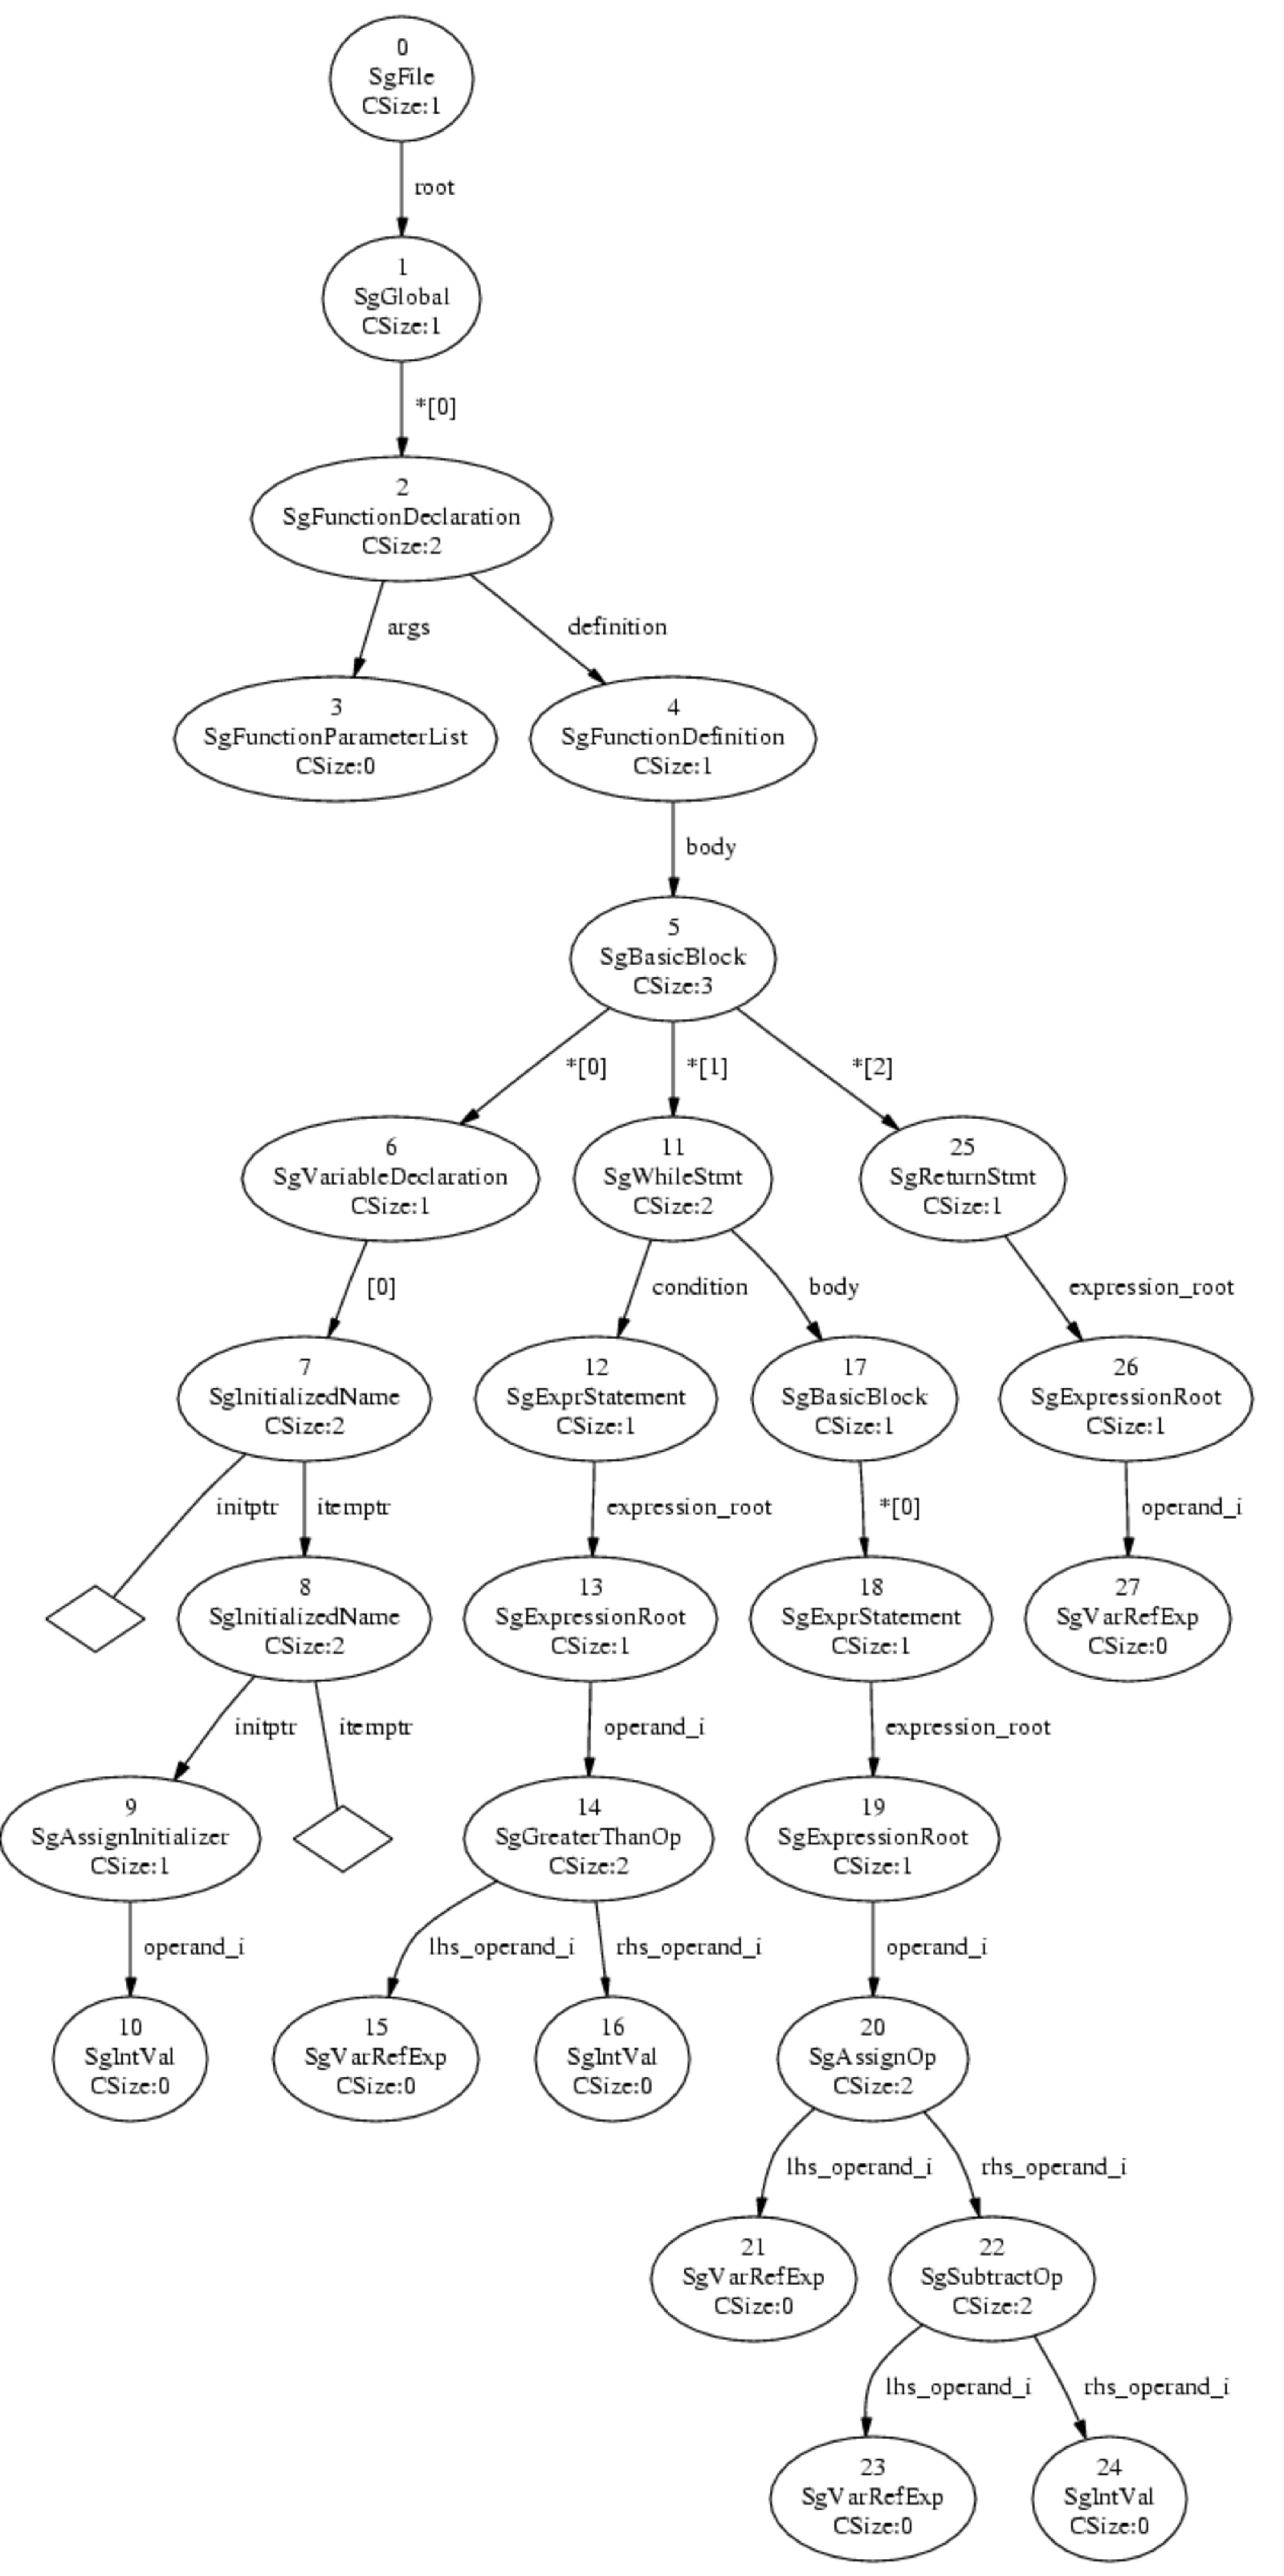
\includegraphics[scale=0.15]{AstProcessing/astprocessingdoc_example1_Preorder}
\caption{Numbers at nodes show the order in which the visit function is called in a preorder traversal}
\label{AstProcessing:PreorderAst}
\end{figure}

\begin{figure}
%\centerline{\psfig{file=AstProcessing/astprocessingdoc_example1.Postorder.ps,height=1.0\linewidth,width=1.0\linewidth,angle=0}}
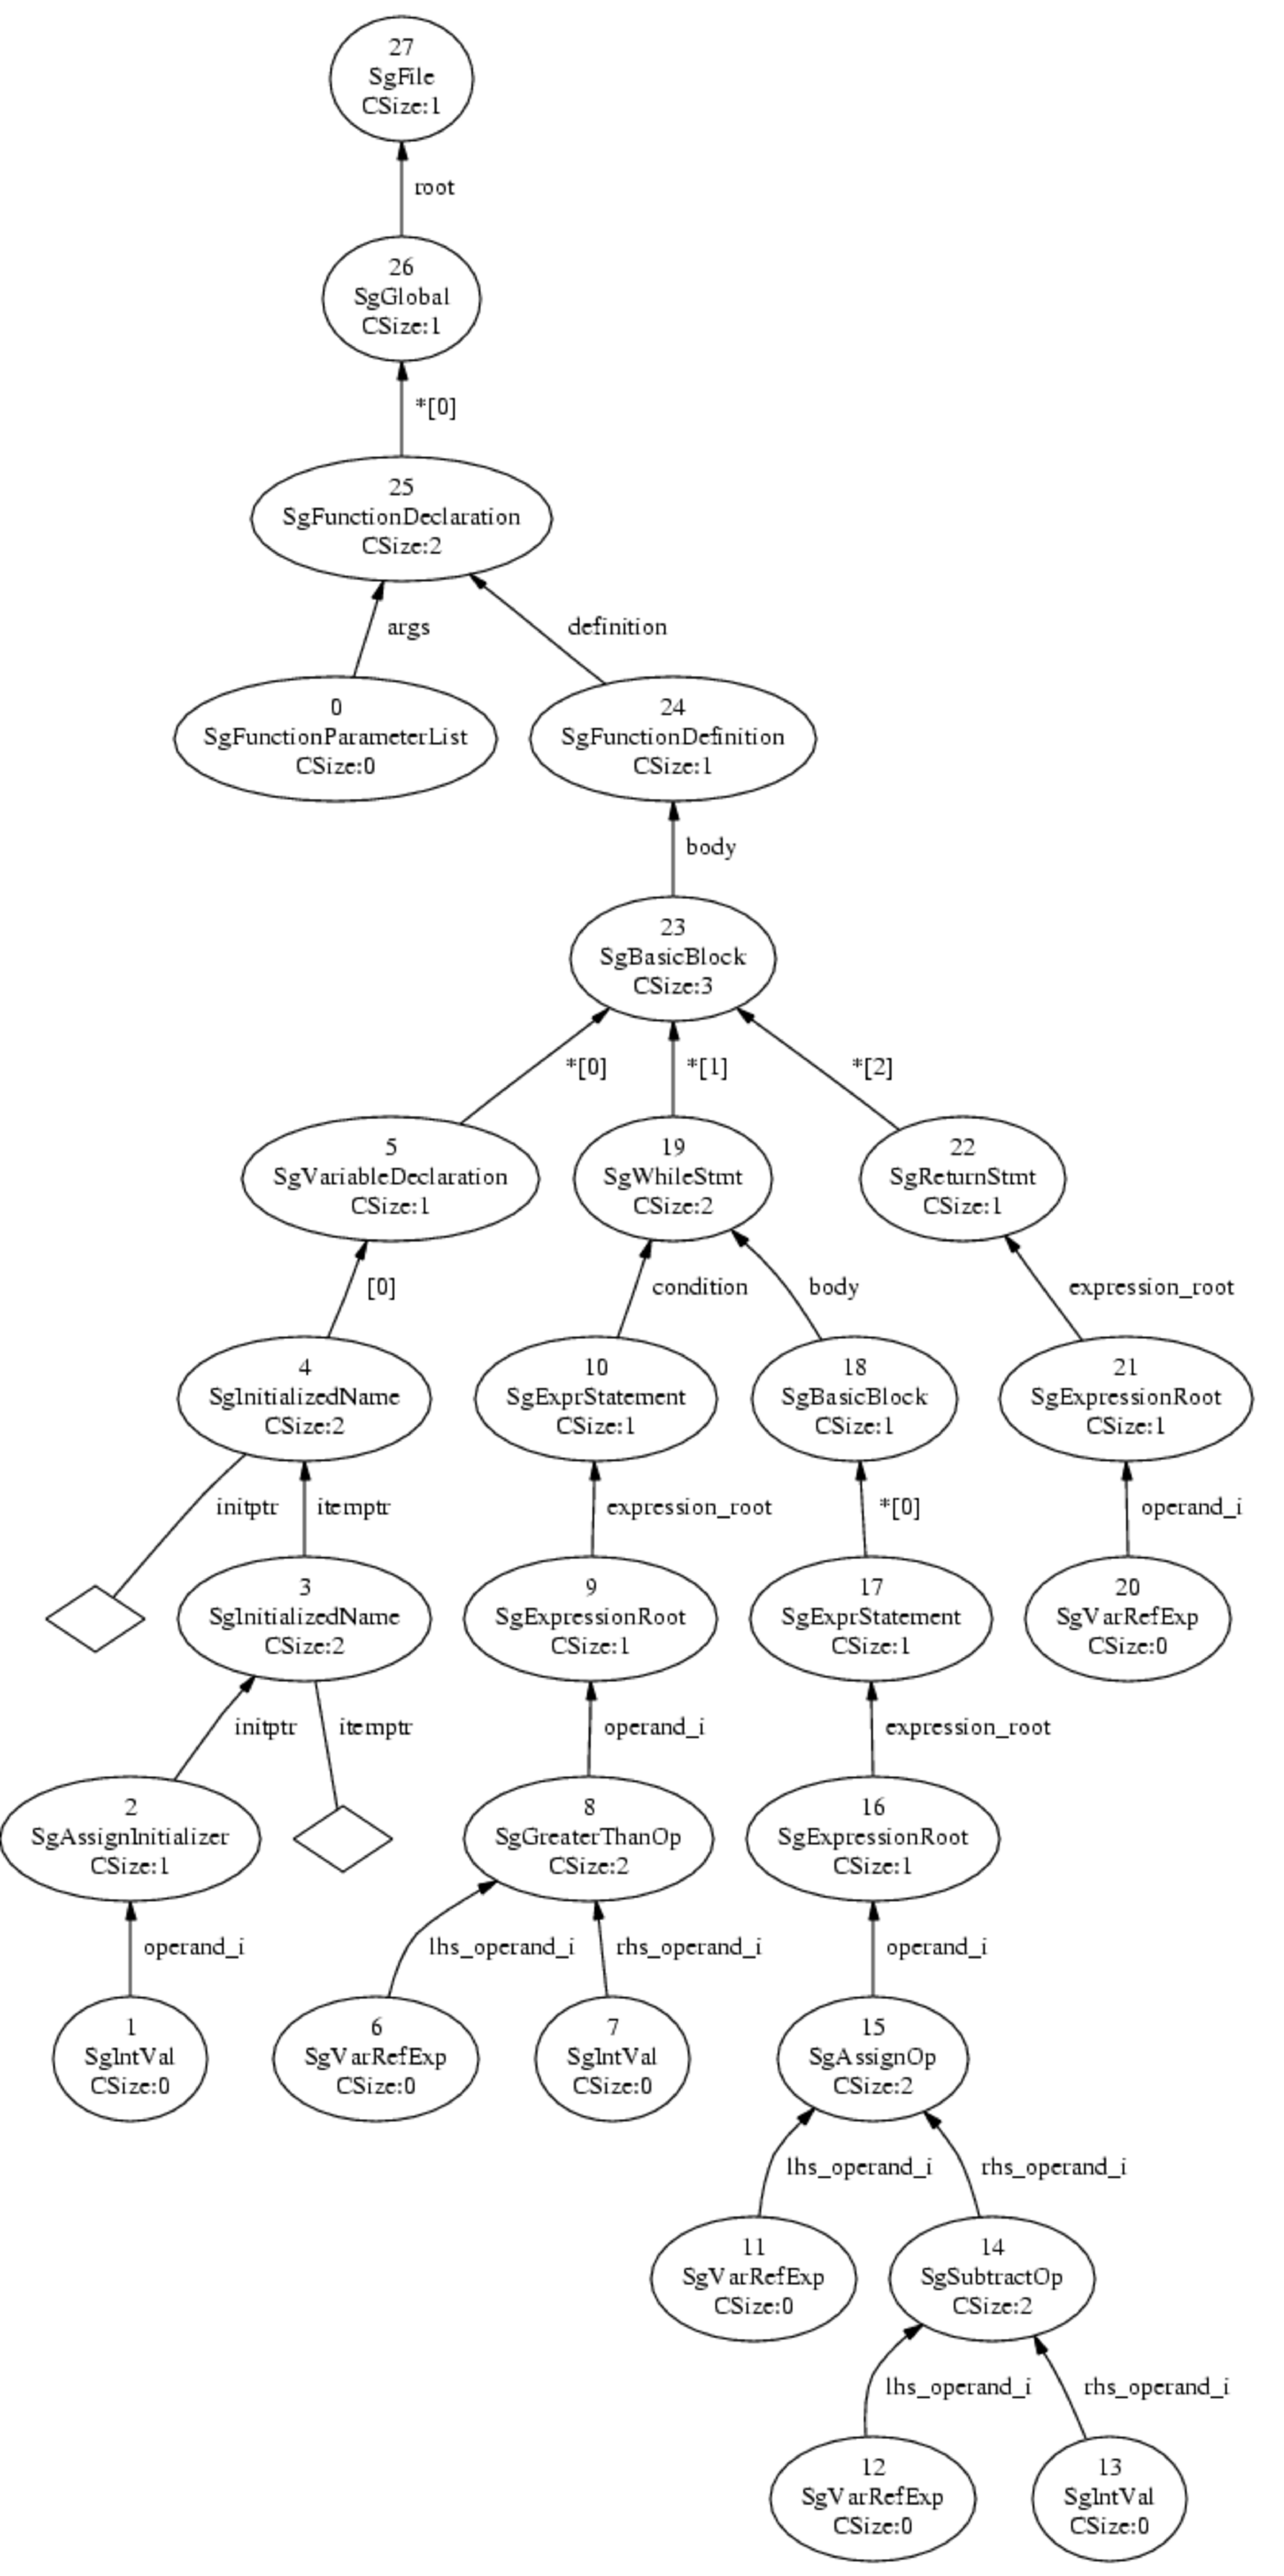
\includegraphics[scale=0.15]{AstProcessing/astprocessingdoc_example1_Postorder}
\caption{Numbers at nodes show the order in which the visit function is called in a postorder traversal}
\label{introduction:PostorderAst}
\end{figure}

The graph shown in figure \ref{AstProcessing:PreorderAst} is the AST of
the program in figure \ref{AstProcessing:example1}. Such an output can
be generated for an AST with:

{\indent
{\mySmallFontSize
\begin{verbatim}
     AstDOTGeneration dotgen;
     dotgen.generateInputFiles(projectNode, AstDOTGeneration::PREORDER);
\end{verbatim}
}}
where {\tt projectNode} is a node of type {\tt SgProjectNode} and the
order in which the AST is traversed is specified to be {\tt
AstDOTGeneration::PREORDER} (or {\tt AstDOTGeneration::POSTORDER}).

\begin{figure}
%\centerline{\psfig{file=AstProcessing/astprocessingdoc_example1.TopDown.ps,height=1.0\linewidth,width=1.0\linewidth,angle=0}}
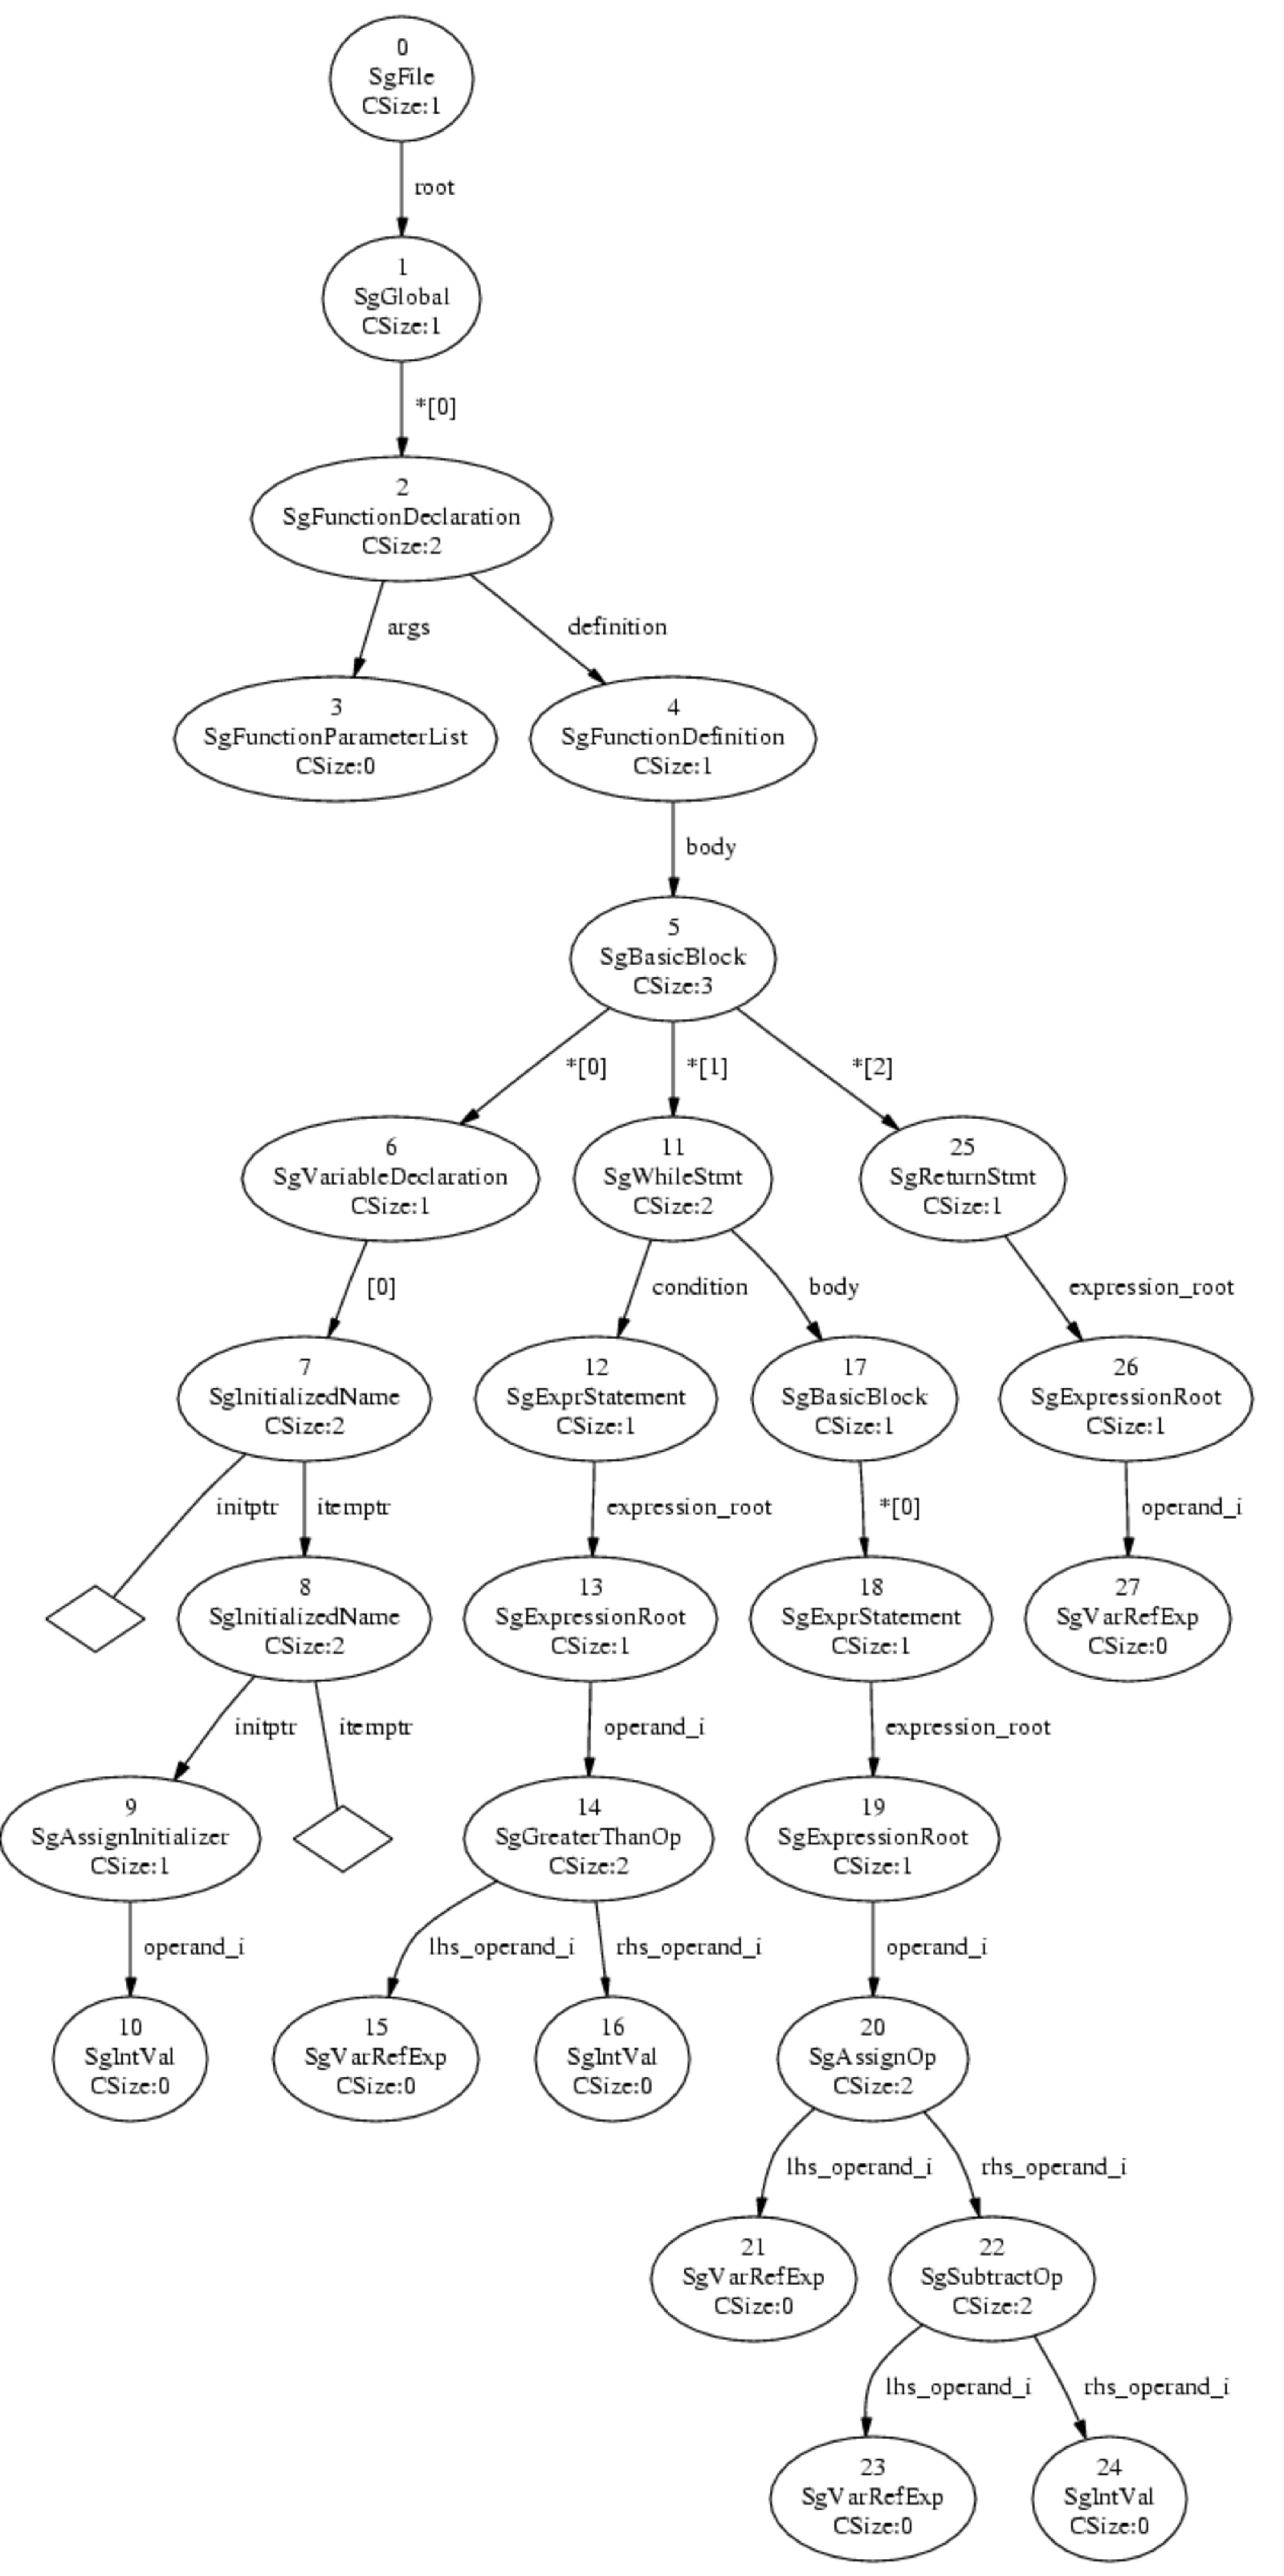
\includegraphics[scale=0.15]{AstProcessing/astprocessingdoc_example1_TopDown}
\caption{Numbers at nodes show the order in which the function evaluateInheritedAttribute is called in a top-down processing}
\label{AstProcessing:TopDownAst}
\end{figure}

\begin{figure}
%\centerline{\psfig{file=AstProcessing/astprocessingdoc_example1.BottomUp.ps,height=1.0\linewidth,width=1.0\linewidth,angle=0}}
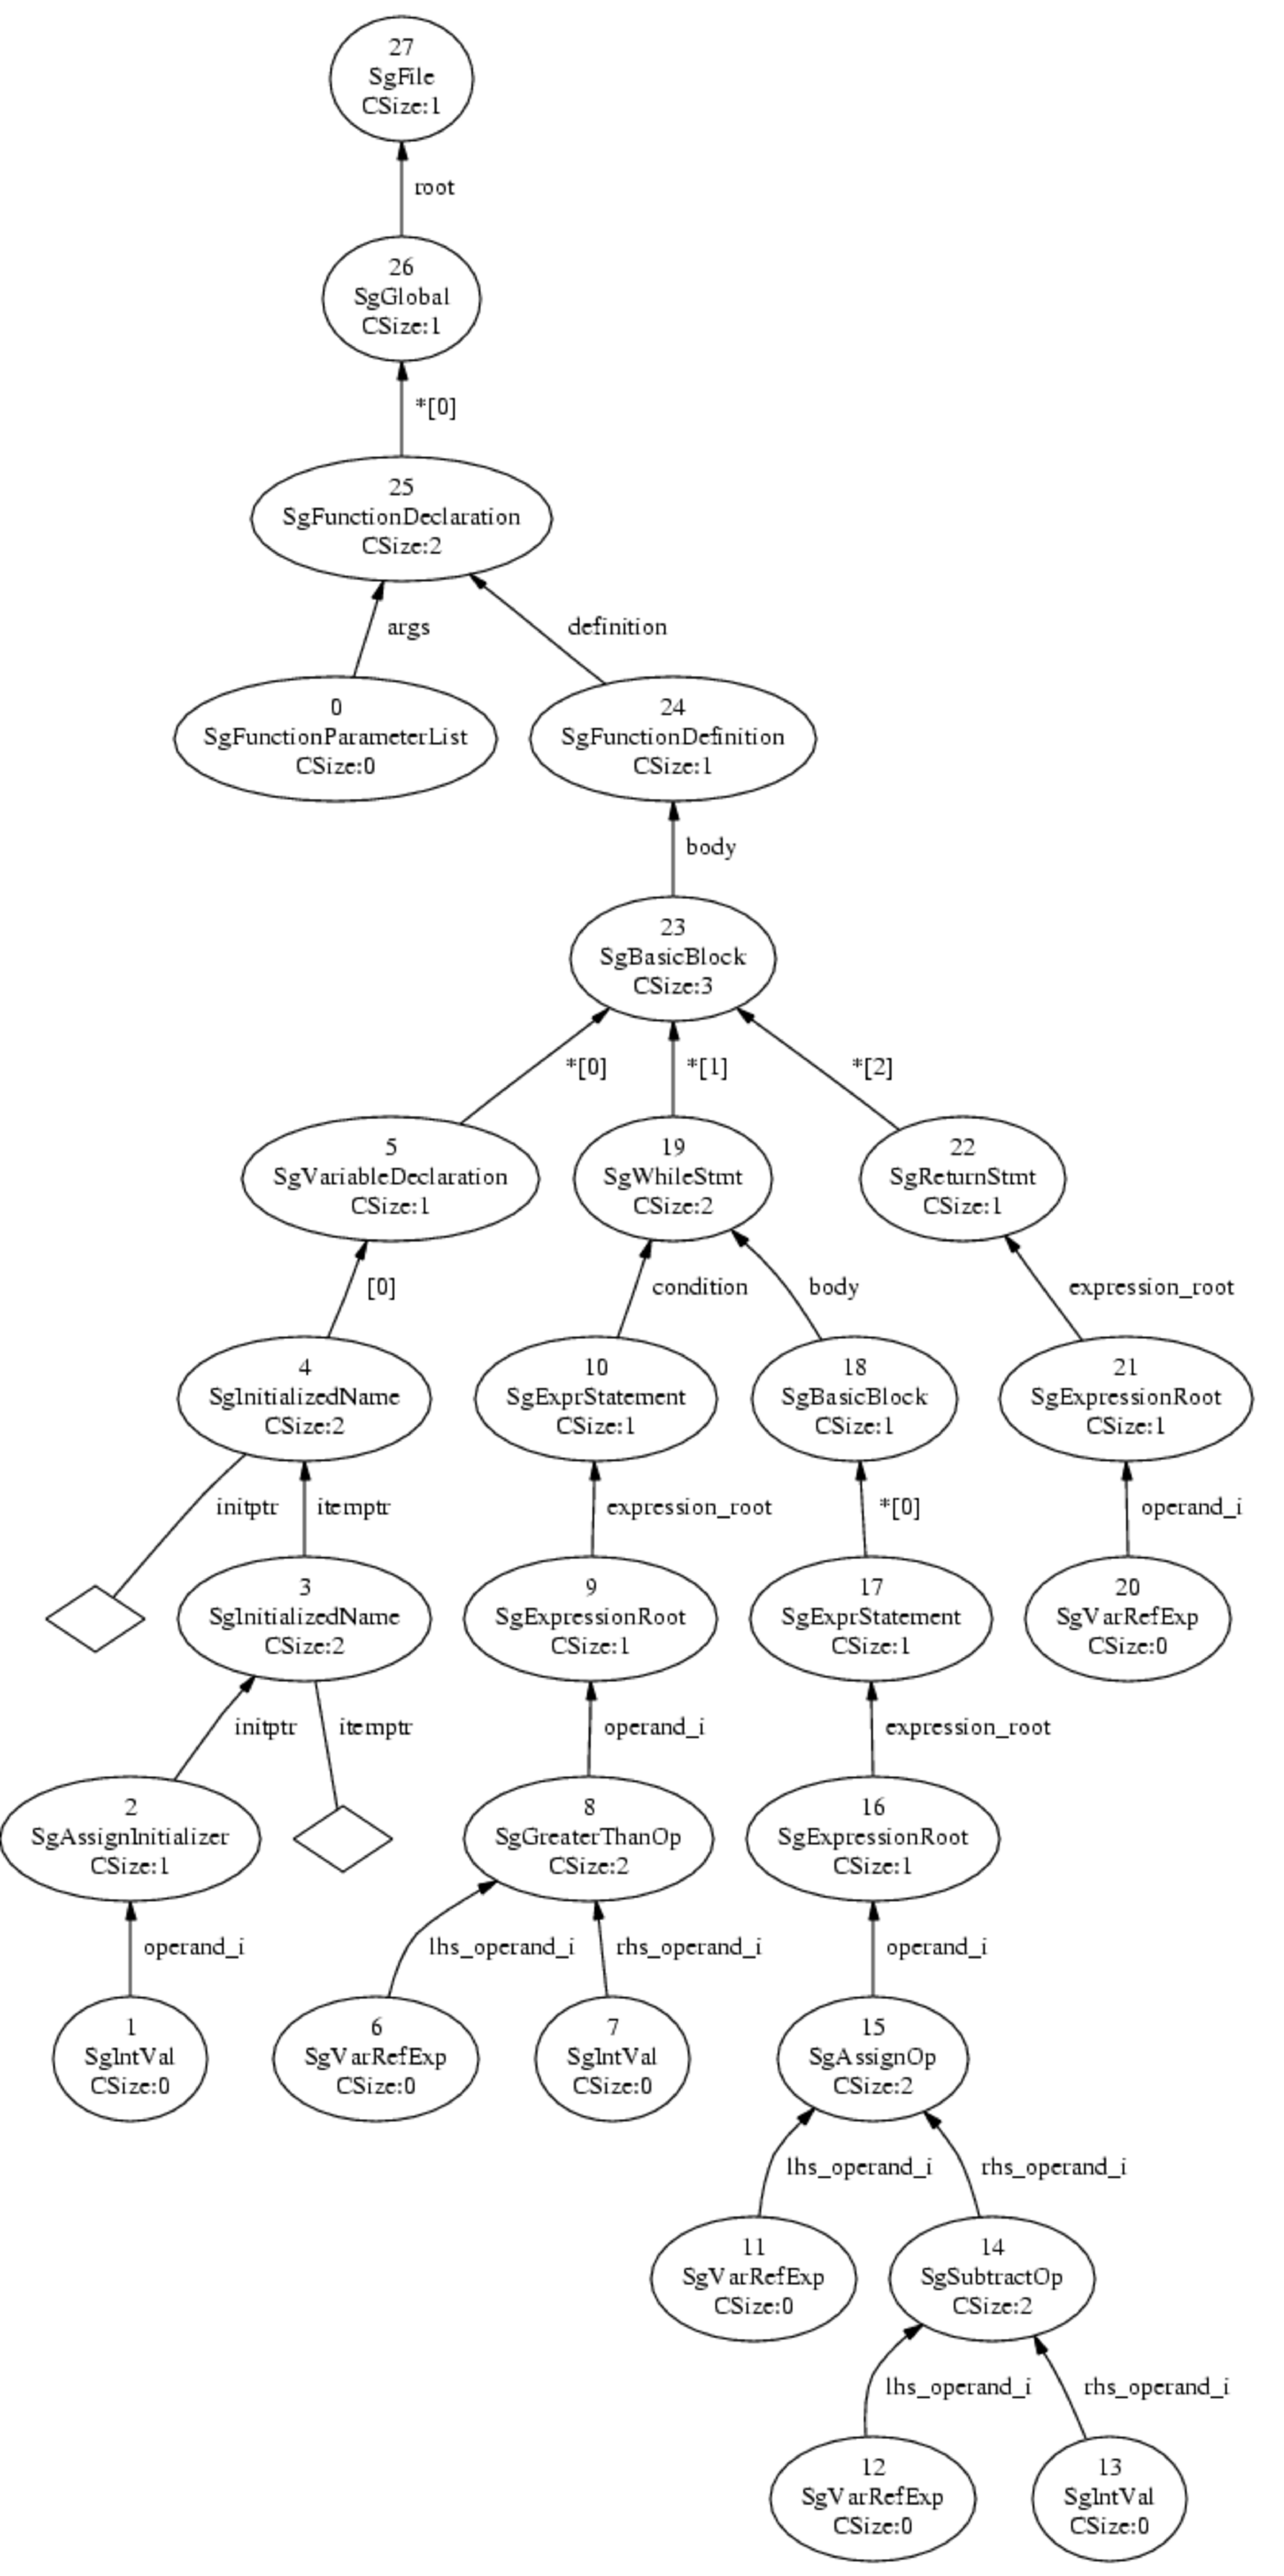
\includegraphics[scale=0.15]{AstProcessing/astprocessingdoc_example1_BottomUp}
\caption{Numbers at nodes show the order in which the function evaluateSynthesizedAttribute is called in a bottom up processing}
\label{AstProcessing:BottomUpAst}
\end{figure}

\begin{figure}
%\centerline{\psfig{file=AstProcessing/astprocessingdoc_example1.TopDownBottomUp.ps,height=1.0\linewidth,width=1.0\linewidth,angle=0}}
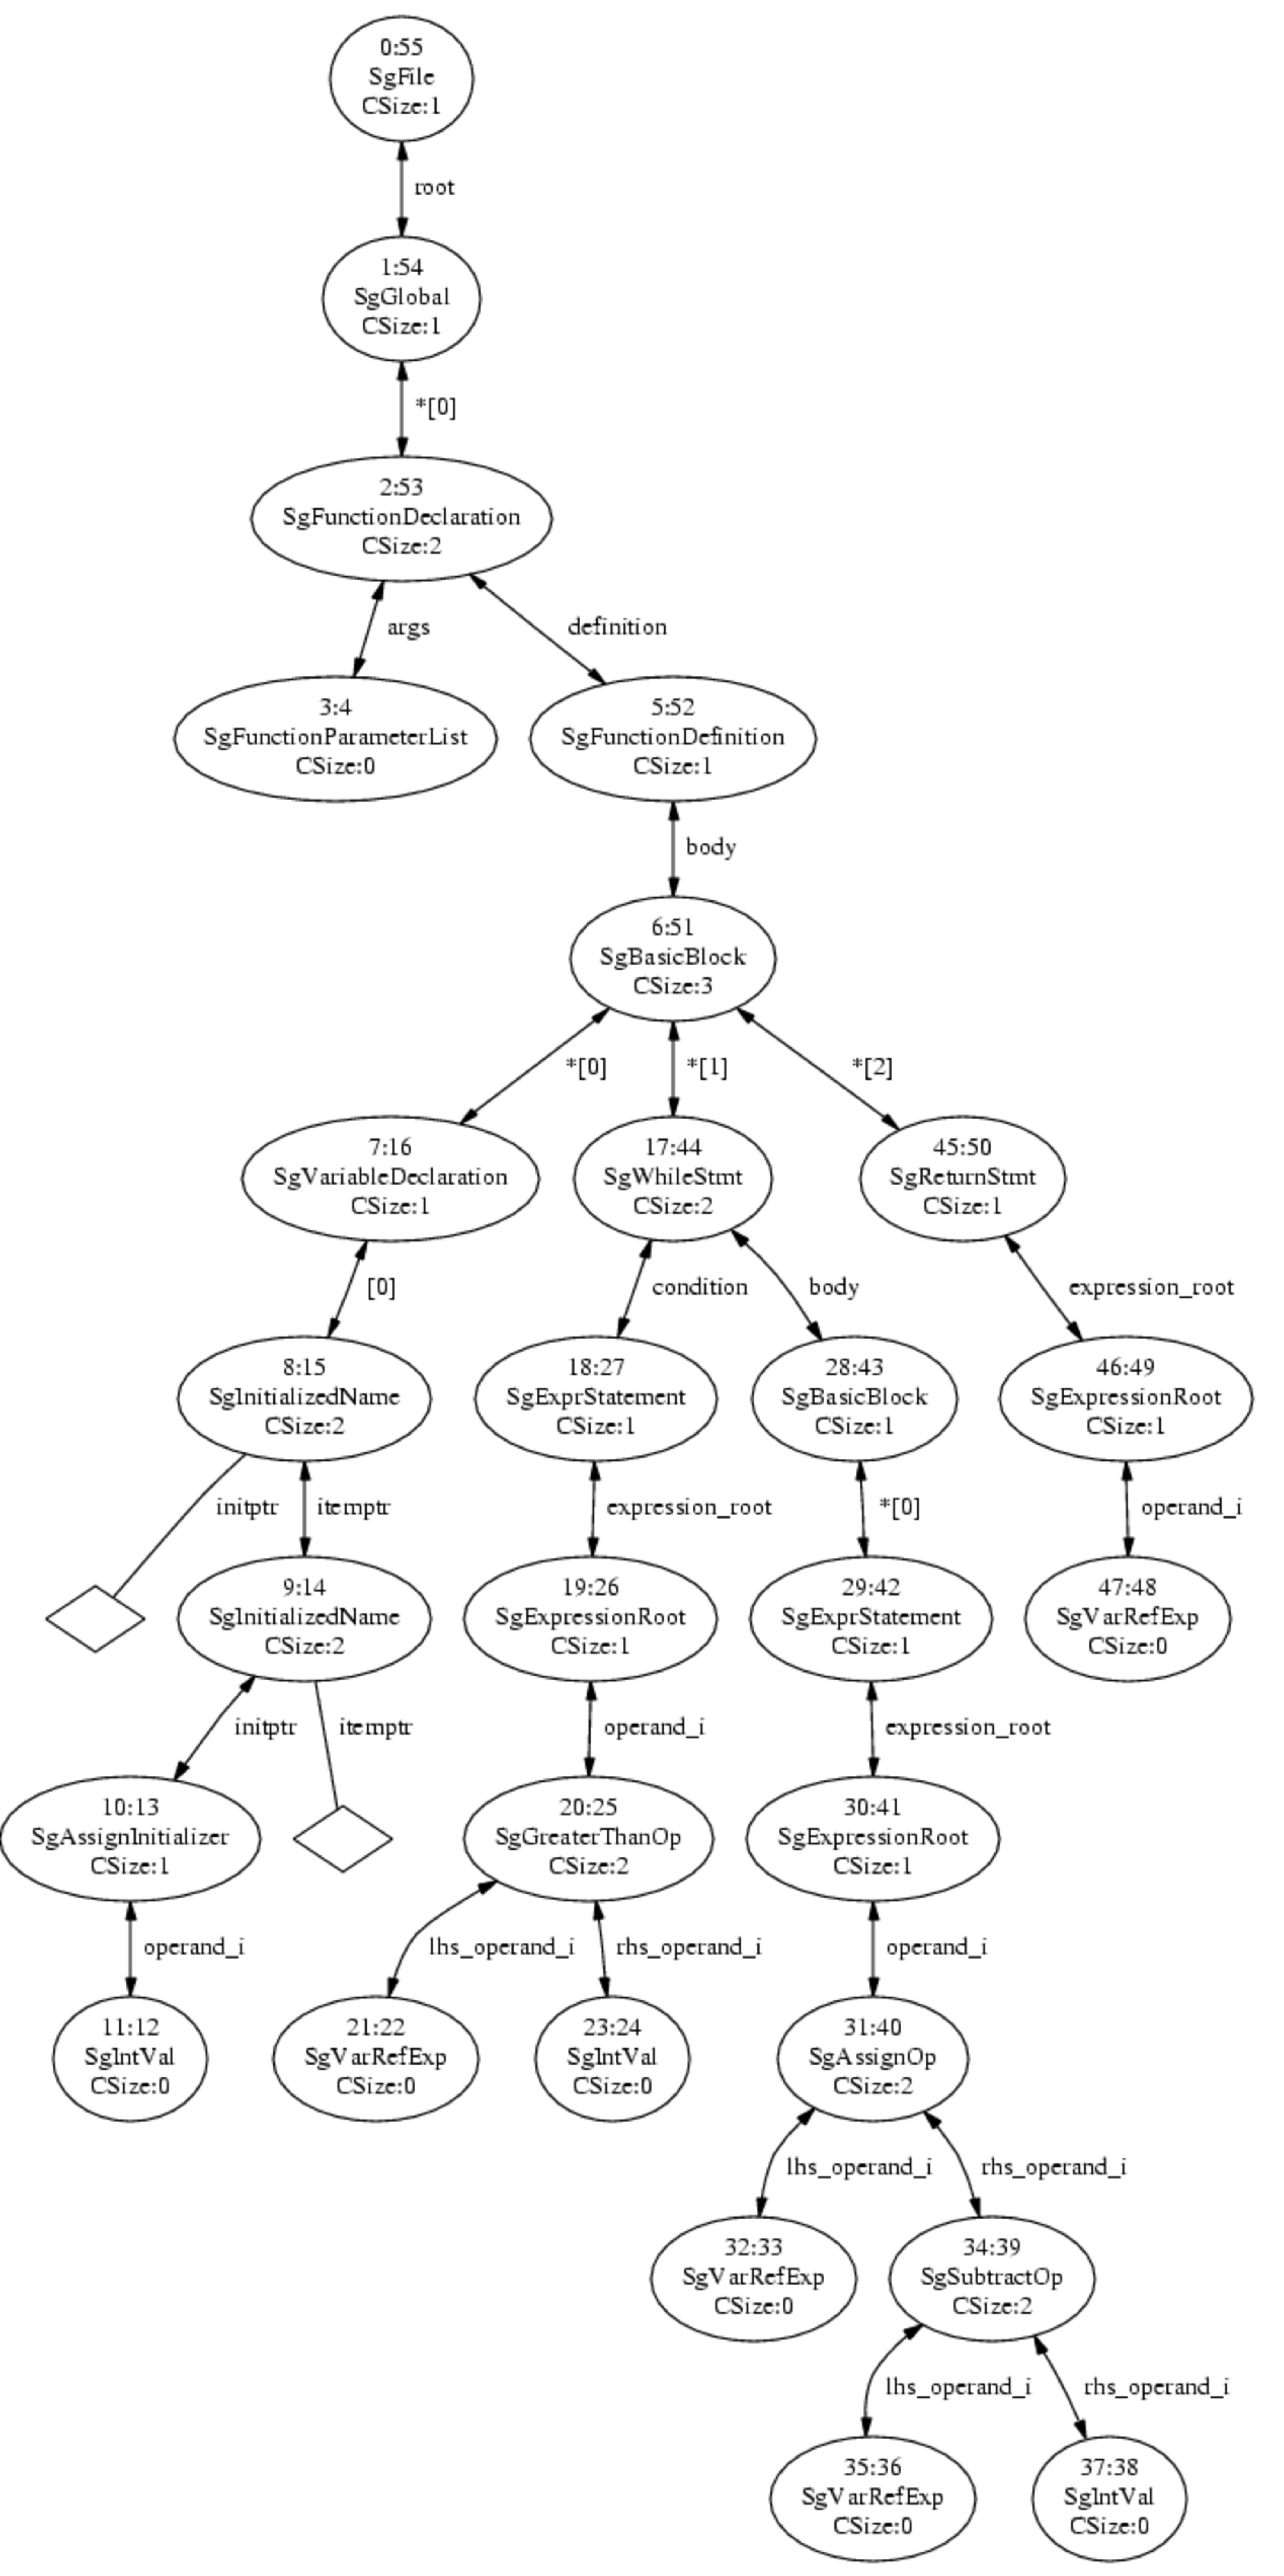
\includegraphics[scale=0.15]{AstProcessing/astprocessingdoc_example1_TopDownBottomUp}
\caption{The pair of numbers at nodes shows the order in which the function
    evaluateInheritedAttribute (first number) and evaluateSynthesizedAttribute (second number)
    is called in a top-down-bottom-up processing.}
\label{AstProcessing:TopDownBottomUpAst}
\end{figure}
%===========================================================================
\section{Conclusions}

All AST*Processing classes provide similar interfaces that differ only by the attributes used. AST node attributes can be used to attach data to each AST node and to share information between different traversals. 

Additional examples for traversal, attributes, pdf, and dot output can be found in 
\begin{itemize}
\item \verb+ROSE/exampleTranslators/documentedExamples/astProcessingExamples+.
\end{itemize}

Table~\ref{tab:sumTraversal} summaries and compares the traversal and query support in ROSE. 
It shows the types of SgNode visited, context, performance, order of nodes being visited, source files being visited, 
and suggested use for each of the choices. 
% Liao 4/21/2010 add a table to summary traversal/query
\begin{table}[htbp]
  \centering
\resizebox{7.0in}{!}{ % width of the table
\begin{tabular}{||l|c|c|c|c|c|c||} \hline
 \multicolumn{7}{||c||}{\textbf{\textcolor{blue}{Regular AST Traversal}}} \\\hline \hline
& \textbf{Node Types} & \textbf{Context} & \textbf{Performance} & \textbf{Order} & \textbf{File Visited} & \textbf{Suggested Use} \\ \hline
%ROSE\_VisitorPattern&  predefined & No & regular & configurable & configuration & Simple traversal \\ \hline
AstSimpleProcessing  &  predefined & No & regular & configurable & configurable & simple analysis \\ \hline
AstPrePostProcessing &  predefined & No & regular & fixed? & configurable & simple analysis \\ \hline
AstTopDownProcessing $<$InheritedAttribute$>$ &  & & &  & &  \\ \hline
AstBottomUpProcessing $<$SynthesizedAttribute$>$ &  & & &  & &  \\ \hline
AstTopDownBottomUpProcessing &  predefined & No & regular & fixed? & configurable & simple analysis \\ \hline
 \multicolumn{7}{||c||}{\textbf{\textcolor{blue}{Combined AST Traversal}}} \\\hline \hline
AstCombinedSimpleProcessing&  & & &  & & \\ \hline
AstCombinedPrePostProcessing&  & & &  & & \\ \hline
AstCombinedTopDownProcessing &  & & &  & & \\ \hline
AstcombinedBottomUpProcessing&  & & &  & & \\ \hline
AstCombinedTopDownBottomUpProcessing &  & & &  & & \\ \hline
 \multicolumn{7}{||c||}{\textbf{\textcolor{blue}{Reverse AST Traversal}}} \\\hline \hline
AstReversePrefixSimpleProcessing &  & & &  & & \\ \hline
AstReversePrefixInhProcessing &  & & &  & & \\ \hline
AstReversePrefixSynProcessing &  & & &  & & \\ \hline
AstReversePrefixInhSynProcessing &  & & &  & & \\ \hline
AstReverseBranchSimpleProcessing &  & & &  & & \\ \hline
AstReverseBranchInhProcessing &  & & &  & & \\ \hline
AstReverseBranchSynProcessing &  & & &  & & \\ \hline
AstReverseBranchInhSynProcessing &  & & &  & & \\ \hline

 \multicolumn{7}{||c||}{\textbf{\textcolor{blue}{Parallel Traversal}}} \\\hline \hline
%& \textbf{Node Type Visited} & \textbf{Context} & \textbf{Performance} & \textbf{Order} & \textbf{File Visited} & \textbf{Suggested Use} \\ \hline
AstSharedMemoryParallelSimpleProcessing &  & & Best &  & & \\ \hline
AstSharedMemoryParallelTopDownProcessing &  & & Best &  & & \\ \hline
AstSharedMemoryParallelBottomUpProcessing &  & & Best &  & & \\ \hline
AstSharedMemoryParallelTopDownBottomUpProcessing &  & & Best &  & & \\ \hline
AstSharedMemoryParallelPrePostProcessing &  & & Best &  & & \\ \hline

AstSharedMemoryParallelizableSimpleProcessing &  & &  Best & & & \\ \hline
AstSharedMemoryParallelizableTopDownProcessing &  & & Best &  & & \\ \hline
AstSharedMemoryParallelizableBottomUpProcessing &  & & Best &  & & \\ \hline
AstSharedMemoryParallelizablePrePostProcessing &  & & Best &  & & \\ \hline
AstSharedMemoryParallelizableTopDownBottomUpProcessing &  & & Best &  & & \\ \hline

 \multicolumn{7}{||c||}{\textbf{\textcolor{blue}{Memory Pool Traversal}}} \\\hline \hline
%& \textbf{Node Type Visited} & \textbf{Context} & \textbf{Performance} & \textbf{Order} & \textbf{File Visited} & \textbf{Suggested Use} \\ \hline
ROSE\_VisitTraversal &  & & better  &  & & \\ \hline
ROSE\_VisitorPattern &  & & better &  & & \\ \hline

 \multicolumn{7}{||c||}{\textbf{\textcolor{blue}{AST Query}}} \\\hline \hline
%& \textbf{Node Type Visited} & \textbf{Context} & \textbf{Performance} & \textbf{Order} & \textbf{File Visited} & \textbf{Suggested Use} \\ \hline
  NodeQuery::querySubTree&  & & &  & & \\ \hline


\end{tabular}
}
\caption{Summary and Comparison of AST Traversals and Queries}
\label{tab:sumTraversal}
\end{table}



\chapter{AST Rewrite Mechanism}

\label{AstRewrite:AstRewrite}

% Purpose:
%\begin{itemize}
%   \item A. Section overview
%   \item B. Why you should read this manual
%   \item C. How to use this manual
%   \item D. Terminology
%   \item E. Overview of library
%   \item F. Program control
%   \item G. Error messages
%   \item H. Section summary
%\end{itemize}
%\begin{center}
%*********************  \newline
%\end{center}
%\vspace{0.25in}

\commentout{
Visionary part not to be included in documentation yet!

     Semantics:
       1) The newest AST is always traversed (rewrite rules are always applied to the
          newest possible AST).
           A) Transformations on header files are seen by the intermediate files in
              subsequent transformations.  In order to make this work we have to write out
              the whole AST.
                a) Optimizations could be done if no header files are transformed, since then
                   the original header files are the same.

    Guiding (problematic) example:
       1) header file (A.h):
             class A { int x; };
          Source file:
             int main () { A a; a.x = 0; }
          Transformation 1:
             Add ``int y;'' to class A (transformation on header file foo.h)
          Transformation 2:
             Add ``a.y = 0;'' to main function

          Transformation 2 depends upon transformation 1 and the intermediate source code
          which specifies transformation 2 requires the updated header file (defined after
          transformation 1).

    Things to do:
        1) Add unparse whole AST to SgFile.
        2) Unparse whole AST and genrate new header files with include statements in the
           source file.

}


% Quote:
% (e.g.) The successful con artist is a mirror of the time and place where he works.

   The Abstract Syntax Tree (AST) Rewrite Mechanism permits modifications 
to the AST.  To effect changes to the input source code, modifications to the 
AST are done by a ROSE translator; and new version of the source code is produced.
% to effect changes to the input source code output as generated source code.  
Although analysis is possible by only reading the AST, transformations (and changes in the
output code from the input code) can only be accomplished by rewriting portions of the AST.
The AST is the single intermediate form manipulated by the preprocessor.  All changes
are eventually output as modifications to the input source code after being processed
through the intermediate form.

% \section{Introduction}
% \label{AstRewrite:introduction}

   The material in this chapter builds on material presented in the previous two
chapters; Writing a Source-to-Source Preprocessor (chapter 
\ref{preprocessorDesign:preprocessorDesign}) and AST Processing 
(chapter \ref{AstProcessing:astProcessing}). This chapter presents the required
AST Rewrite Traversal and the simple interface functions to the {\tt AST\_Rewrite} class.  
A section is included that 
demonstrates code that rewrites the AST for any input code. More complex examples are
possible but each uses the AST Rewrite Mechanism in a similar way.  The ROSE Tutorial 
documents a few more interesting examples.% \ref{RoseExamples:RoseExamples}.

\section{Introduction}

   The rewrite mechanism in ROSE contains four different levels of interface
within its design.  Table \ref{tab:RewriteInterface} shows the different levels of
the interface design for the ROSE rewrite mechanism.  Each level consists of
simple tree editing operations ({\tt insert()}, {\tt replace()}, and 
{\tt remove()}) that can operate on statements within the AST.

\begin{table}[htb]
{\begin{center}
    \renewcommand{\arraystretch}{1.25}

\begin{tabular}{|c|c|c|l|}
\hline
\multirow{3}{35mm}{Relative Positioning (contains state)} 
     & \multirow{3}{15mm}{String-Based} 
          & \multirow{3}{35mm}{High Level Interface (level 4)} 
               & {insert(SgNode*,string,scope,location)} \\
     & {} & {} & {replace(SgNode*,string,scope,location)} \\
     & {} & {} & {remove(SgNode*)} \\\hline
\multirow{9}{35mm}{Absolute Positioning (contains no state)} 
     & \multirow{3}{15mm}{String-Based} 
          & \multirow{3}{35mm}{Mid Level Interface (level 3)} 
          & {insert(SgNode*,string,location)} \\ 
     & {} & {} & {replace(SgNode*,string,location)} \\
     & {} & {} & {remove(SgNode*)} \\\cline{2-4}
     & \multirow{6}{15mm}{SgNode*} 
          & \multirow{3}{35mm}{Low Level Interface (level 2)} 
          & {insert(SgNode*,SgNode*)} \\ 
     & {} & {} & {replace()} \\
     & {} & {} & {remove(SgNode*)} \\\cline{3-4}
     & {} & \multirow{3}{35mm}{SAGE III Interface (level 1)} 
          & {insert(SgNode*,SgNode*)} \\ 
     & {} & {} & {replace(SgNode*,SgNode*)} \\ 
     & {} & {} & {remove(SgNode*)} \\\hline 
\end{tabular}

 \end{center}
}
  \caption{Different levels of the ROSE Rewrite mechanism.}
  \label{tab:RewriteInterface}
\end{table}

% Many attempts to input source code from files
% \verbatiminput{\AstRewriteExampleDirectory/testExample1.C}
% \verbatiminput{/home/dquinlan/ROSE/NEW_ROSE/AST_RewriteMechanism/testExample1.C}
% \verbatimfiles{/home/dquinlan/ROSE/NEW_ROSE/AST_RewriteMechanism/testExample1.C}
% \verbatimlisting{/home/dquinlan/ROSE/NEW_ROSE/AST_RewriteMechanism/testExample1.C}
% \begin{listing}
%     testExample1.C
% \end{listing}
% \listinginput{5}{/home/dquinlan/ROSE/NEW_ROSE/AST_RewriteMechanism/testExample1.C}

\section{Multiple Interfaces to Rewrite Mechanism}

   There are four different levels of interfaces in the rewrite mechanism
because there are many different program transformations requirements.  Each level
builds on the lower level, and the highest level interface is the most sophisticated 
internally. Each interface has only three functions: {\tt insert()}, {\tt replace()}, 
and {\tt remove()}.

\subsection{SAGE III Rewrite Interface}
   This lowest possible level of interface is implemented as member functions on the
SgNode objects. It is used interanlly to implement the higher level interfaces (including
the Low Level Rewrite Interface.  Uniformally,
operations of {\tt insert()}, {\tt replace()}, and {\tt remove()} apply only to SAGE III 
objects representing containers (SAGE III objects that have containers internally, 
such as SgGlobal, SgBasicBlock, etc.).  Strings cannot be specified at this level of
interface; only subtrees of the AST may be specified.  New AST fragments must be
built separately and may be inserted or used to replace existing AST subtrees in the AST.
Operations using this interface have the following properties:
\begin{itemize}
   \item Operations performed on collections only.
   \item Operations are immediate executed.
   \item Operations are local on the specified node of the AST.
   \item Operations do not take attached comments or preprocessor directives into account. \\
    This can lead to unexpected results (e.g. removing or moving {\tt \#include} directives
    by accident).
\end{itemize}

\subsection{Low Level Rewrite Interface}
    This interface is similar to the SAGE III Rewrite Interface except that operations
are performed on any statement and not on the containers that store the statement lists.
The domain of the operations -- on the statements instead of on the parent nodes of the 
statements -- is the most significant difference between the two interfaces.  An additional
feature includes support for repositioning attached comments/directives from removed
nodes to their surrounding nodes to preserve them within {\tt replace()} and 
{\tt remove()} operations.  Additional support is provided for marking inserted statements
as transformations within the Sg\_File\_Info objects.
Operations using this interface have the following properties:
\begin{itemize}
   \item Attached comments/directives are relocated.
   \item Inserted AST fragments are marked within the Sg\_File\_Info objects.
   \item Operations are immediate.
   \item Operations are local on the specified node of the AST.
\end{itemize}

\subsection{Mid Level Rewrite Interface}
    This interface builds on the low-level interface and adds the string interface,
which permits simpler specification of transformations.
Operations using this interface have the following properties:
\begin{itemize}
   \item Strings used to specify transformations.
   \item Operations are immediate.
   \item Operations are local on the specified node of the AST.
\end{itemize}

\subsection{High Level Rewrite Interface}
    This interface presents the same string based rewrite mechanism as the mid-level
interface but adds additional capabilities.
This interface is the most flexible rewrite interface within ROSE.  Although it 
must be used within a traversal to operate on the AST, it provides a mechanism to express
more sophisticated transformations with less complexity due to its support of relative 
positioning of transformation strings within the AST (relative to the current node within
a traversal). 

    The high-level rewrite mechanism uses the same three functions as the other rewrite
interfaces, but with an expanded range of enum values to specify the intended scope
and the location in that scope.  The scope is specified using the ScopeIdentifierEnum
type defined in the HighLevelCollectionTypedefs class. These enum values are:
\begin{itemize}
   \item unknownScope
   \item LocalScope 
   \item ParentScope 
   \item NestedLoopScope
   \item NestedConditionalScope
   \item FunctionScope
   \item FileScope
   \item GlobalScope
   \item Preamble
\end{itemize}
The position in any scope is specified by the PlacementPositionEnum
type, which is defined in the HighLevelCollectionTypedefs class. 
These enum values are:
\begin{itemize}
     \item PreamblePositionInScope
     \item TopOfScope
     \item TopOfIncludeRegion
     \item BottomOfIncludeRegion
     \item BeforeCurrentPosition
     \item ReplaceCurrentPosition
     \item AfterCurrentPosition
     \item BottomOfScope
\end{itemize}

Function prototypes of interface functions:
{\indent
{\mySmallFontSize
\begin{verbatim}
   void insert (SgNode*, string ,HighLevelCollectionTypedefs::ScopeIdentifierEnum,HighLevelCollectionTypedefs::PlacementPositionEnum);
\end{verbatim}
}}
Example of how to use specific insertion of transformation into the AST (required traversal not shown):
{\indent
{\mySmallFontSize
\begin{verbatim}
   insert (astNode, ``int x;'' ,HighLevelCollectionTypedefs::FunctionScope,HighLevelCollectionTypedefs::TopOfScope);
\end{verbatim}
}}
Operations using this interface have the following properties:
\begin{itemize}
   \item Adds relative positioning to the specification of transformations.
   \item Requires traversal for operation on the AST.
   \item Operations are delayed and occur durring the required traversal, all operations
    are completed by the end of the traversal.
   \item Operations occure on AST nodes along a path defined by the chain from the current
    input node to the operator to the root node of the AST (SgProject).
\end{itemize}



\subsection{Advantages and Disadvantages of Rewrite Interfaces}

   Each interface builds upon the lower level interfaces and each 
has some advantages and disadvantages. Table 
\ref{tab:RewriteInterfaceAdvantagesDisadvantages} lists the
major features and requirements associated with each.  The
high-level interface (Level 4) presents the most sophisticated 
features, but only works as part of a traversal of the AST.  The 
mid-level interface is the lowest level interface that permits 
the specification of transformations as strings.  The low-level interface
is useful when AST fragments are built directly using the SAGE III
classes through their constructors (a somewhat tedious process).
The low level interface preserves the original interfaces adopted 
from SAGE II.

\begin{table}[htb]
{\begin{center}
    \renewcommand{\arraystretch}{1.25}

\begin{tabular}{|c|c|c|c|c|}
\hline
 {Interface:Features} & {Contains State}  & {Positioning} & {String} & {Traversal} \\\hline
     Level 1 & No State &  Absolute  & AST Subtree & Not Used    \\
     Level 2 & No State &  Absolute  & AST Subtree & Not Used    \\
     Level 3 & No State &  Absolute  &    String   & Not Used    \\
     Level 4 &  State   &  Relative  &    String   & Required    \\
\hline
\end{tabular}

 \end{center}
}
  \caption{Advantages and disadvantages of different level interfaces 
           within the ROSE Rewrite Mechanism.}
  \label{tab:RewriteInterfaceAdvantagesDisadvantages}
\end{table}

\section{Generation of Input for Transformation Operators}
    Providing operators to {\tt insert()}, {\tt replace()}, {\tt remove()}
solves only part of the problem of simplifying transformations.  The other part 
of the problem is generating the input to the transformation operators.  Both 
{\tt insert()} and {\tt replace()} require input, either as an AST fragement or
as a string containing source code.  This section presents the pros and cons of the
specification of transformations as strings.

\subsection{Use of Strings to Specify Transformations}

    The mid-level and high-level rewrite interfaces introduce the use of
strings to specify transformations.  Using strings to specify transformations 
attempts to define a simple mechanism for a non-compiler audience 
to express moderately complex transformations.  The alternative is to build the
AST fragments to be inserted directly using SAGE III and the constructors
for its objects.  In general, the direct construction of AST fragments
is exceedingly tedious, and while aspects can be automated, the most
extreme example of this automation is the AST constructions from source 
code strings.  A disadvantage is that the generation of the AST fragment
from strings is slower, but it is only a compile-time issue.

\subsection{Using SAGE III Directly to Specify Transformations}

   It is possible to build AST fragments directly using SAGE III and insert these into
the AST.  This alternative to the use of strings is more complex and is only
briefly referenced in this section.

   The constructors for each of the SAGE III objects form the user interface required to
build up the ASTfragments.  The documentation for these appear in the reference chapter
of this manual.

A few notes:
\begin{enumerate}
 \item Use the {\tt Sg\_File\_Info* Sg\_File\_Info::generateDefaultFileInfoForTransformationNode();} 
static member function to generate the Sg\_File\_Info object required for each of the
constructor calls.  This marks the IR nodes as being part of a transformation and signals
that they should be output within code generation (unparsing).
\end{enumerate}


\section{AST Rewrite Traversal of the High-Level Inteface}

    The AST Rewrite Mechanism uses a traversal of the AST, similar to the
design of a traversal using the AST Processing 
(Chapter \ref{AstProcessing:astProcessing}) part of ROSE.
The example code \ref{AstRewrite:example1} specifically shows an {\bf AstTopDownBottomUpProcessing}
\ref{AstProcessing:AstTopDownBottomUpProcessing}
traversal of the AST.  Using conditional compilation,
the example code shows the somewhat trivial changes required to convert
a read-only AST traversal into a read-write AST rewrite operation. In this
example the AST traversal is converted to be ready for rewrite operations, but
no rewrite operations are shown. The purpose of this example is only to show the
modifications to an existing traversal that are required to use the AST rewrite
mechanism.

   The specialized AST rewrite traversal is internally derived from the ASTProcessing
{\bf TopDownBottomUp} traversal (processing) but adds additional operations
in recording the local context of source code position (in the inherited attribute)
and performs additional operations on the way back up the AST (on the synthesized attribute).

% \vspace{0.5in}

% A note to the reader about a difference between the two versions
% of the documentation that we generate.
\begin{latexonly}
% This listing appears in B\&W within the html version of the documentation.
\end{latexonly}
\begin{htmlonly}
% This listing appears in color within the generated latex postscript document.
\end{htmlonly}
% This reference doesn't seem to work properly.
% See link to postscript documentation at \ref{Rose:postscriptVersionOfUserManual}.

% DQ (9/12/2006): If we make this a figure then it will overflow the page.
% maby we should split this figure into two pieces (as is done in the ROSE tutorial for
% some of the longer examples there.
% \begin{figure}[tb]
{\indent
{\mySmallFontSize
\label{AstRewrite:exampleShowingModificationsToUseAstRewriteMechanism}
% Do this when processing latex to generate non-html (not using latex2html)
\begin{latexonly}
   \lstinputlisting{\AstRewriteExampleDirectory/astRewriteExample1.C}
\end{latexonly}
% Do this when processing latex to build html (using latex2html)
\begin{htmlonly}
   \verbatiminput{\AstRewriteExampleDirectory/astRewriteExample1.C}
\end{htmlonly}
%end of scope in font size
}
% End of scope in indentation
}
% \caption{ Example of now to use AST Rewrite Mechanism. }
% \label{AST_Code}
% \end{figure}

\fixme{This should be a figure that fits onto a single page.}

\commentout{
\begin{latexonly}
\begin{figure}[tb]
\begin{center}
\begin{tabular}{|c|} \hline
     Example Showing AST Rewrite Traversal
\\\hline\hline

% \lstinputlisting{/home/dquinlan/ROSE/NEW_ROSE/AST_RewriteMechanism/testExample1.C}
\lstinputlisting{\AstRewriteExampleDirectory/astRewriteExample1.C}

\\\hline
\end{tabular}
\end{center}
\caption{ Example of now to use AST Rewrite Mechanism. }
\label{AST_Code}
\end{figure}
\end{latexonly}
}

   This example shows the setup required to use the AST Rewrite Mechanism.
The next section shows how to add new code to the AST.  The {\tt main()}
function is as in example of how to use a traversal (see chapter 
\ref{preprocessorDesign:AstTraversalPreprocessor}).

   Note that the differences between the traversal required for use
with the AST Rewrite Mechanism is different from the traversals associated
with \ref{AstProcessing:AstTopDownBottomUpProcessing}.  The exact differences
are enabled and disabled in the example
\ref{AstRewrite:exampleShowingModificationsToUseAstRewriteMechanism}
by setting the macro {\tt USE\_REWRITE\_MECHANISM} to zero (0) or one (1).

   The differences between traversals using
{\tt AstTopDownBottomUpProcessing<InheritedAttrbute,SynthesizedAttribute>}
and traversals using the AST Rewrite Mechanism (
{\tt AST\_Rewrite::RewriteTreeTraversal<InheritedAttrbute,SynthesizedAttribute>})
are both required to use the AST Rewrite Mechanism. They are:
\begin{enumerate}
     \item InheritedAttributes must derive from {\tt AST\_Rewrite::InheritedAttribute}.
     \item Must define constructor {\tt InheritedAttribute::InheritedAttribute(SgNode* astNode)}.
     \item Must define copy constructor: \\
              {\tt InheritedAttribute::InheritedAttribute(const InheritedAttribute \& X, SgNode* astNode)}.
     \item SynthesizedAttribute must derive from {\tt AST\_Rewrite::SynthesizedAttribute}
     \item Must derive new traversal from \\ 
              {\tt AST\_Rewrite::RewriteTreeTraversal<InheritedAttrbute,SynthesizedAttribute>})
           instead of \\
              {\tt AstTopDownBottomUpProcessing<InheritedAttrbute,SynthesizedAttribute>}.
\end{enumerate}


\section{Examples}
    This section presents several examples using the different interfaces
to specify simple transformations.  

\commentout{
\subsection{SAGE III Interface Example}

\fixme{Incomplete documentation.}

\subsection{Low-Level Interface Example}

\fixme{Incomplete documentation.}

\subsection{Mid-Level Interface Example}

\fixme{Incomplete documentation.}

\subsection{High-Level Interface Example}

\fixme{Incomplete documentation.}
}

\subsection{String Specification of Source Code}
    Both the mid-level and high-level interfaces use strings to
specify source code. The examples below show how to specify 
the strings.
\subsubsection{Specification of Source Code}
    Specification of source code is straight forward.
However, quoted strings must be escaped and strings spanning
more then one line must use the string continuation character ("$\backslash$").
\begin{itemize}
   \item {\tt MiddleLevelRewrite::insert(statement,"int newVariable;",locationInScope);}
   \item {\tt MiddleLevelRewrite::insert(statement,"timer($\backslash$"functionName$\backslash$");",locationInScope);}
   \item {\tt MiddleLevelRewrite::insert(statement,\\ "/* Starting Comment */
    $\backslash$n $\backslash$\\ int y; { int y; } for (y=0; y < 10; y++){z = 1;}
    $\backslash$n $\backslash$\\ /* Ending Comment */$\backslash$n",locationInScope);}
\end{itemize}

\subsubsection{Specification of CPP Directives}
    Specification of CPP directives as strings is as one would expect
except that where quotes ("") appear in the string they must be escaped
($\backslash$"$\backslash$") to remain persistent in the input string.
\begin{itemize}
   \item {\tt MiddleLevelRewrite::insert(statement,"\#define TEST",locationInScope);}
   \item {\tt MiddleLevelRewrite::insert(statement,"\#include<foo.h>",locationInScope);}
   \item {\tt MiddleLevelRewrite::insert(statement,"\#include $\backslash$"foo.h$\backslash$"",locationInScope);}
\end{itemize}

\subsubsection{Specification of Comments}
    Specification of comments are similar.
\begin{itemize}
   \item {\tt MiddleLevelRewrite::insert(statement,"/* C style comment test */",locationInScope);}
   \item {\tt MiddleLevelRewrite::insert(statement,"// C++ comment test ",locationInScope);}
\end{itemize}

\subsubsection{Specification of Macros}
    The specification of macros is similar to CPP directives
except that longer macros often have line continuation and formatting.
We show how to preserve this in the example macro definition below.
Transformation involving the use of a macro is more complex if the
macro call is to be preserved in the final transformation 
(left unexpanded in the generation of the AST fragment with the 
rewrite mechanism).

\paragraph{Macro Definition:}
   A macro definition is similar to a CPP directive. The long example is taken from the
Tuning Analysis Utilities (TAU) project which instruments code with similar macro calls.
\begin{itemize}
   \item {\tt MiddleLevelRewrite::insert(statement,"\#include<foo.h>",locationInScope);}
   \item {\tt MiddleLevelRewrite::insert(statement,"\#include $\backslash$"foo.h$\backslash$"",locationInScope);}
   \item {\tt MiddleLevelRewrite::insert(statement,"\#define PRINT\_MACRO(name) name;",locationInScope);}
   \item {\tt MiddleLevelRewrite::insert(statement,\\
"$\backslash$n$\backslash$\\
\#ifdef USE\_ROSE$\backslash$n$\backslash$\\
// If using a translator built using ROSE process the simpler tauProtos.h header  $\backslash$n$\backslash$\\
// file instead of the more complex TAU.h header file (until ROSE is more robust) $\backslash$n$\backslash$\\
   \#include $\backslash$"tauProtos.h$\backslash$"$\backslash$n$\backslash$n\\
// This macro definition could be placed into the tauProtos.h header file $\backslash$n$\backslash$\\
   \#define TAU\_PROFILE(name, type, group) $\backslash$$\backslash$$\backslash$n$\backslash$\\
        static TauGroup\_t tau\_gr = group; $\backslash$$\backslash$$\backslash$n$\backslash$\\
        static FunctionInfo tauFI(name, type, tau\_gr, \#group); $\backslash$$\backslash$$\backslash$n$\backslash$\\
        Profiler tauFP(\&tauFI, tau\_gr); $\backslash$n$\backslash$\\
\#else$\backslash$n$\backslash$\\
   \#include $\backslash$"TAU.h$\backslash$"$\backslash$n$\backslash$\\
\#endif"$\backslash$$\backslash$\\
,locationInScope);}
\end{itemize}

\paragraph{Macro Use:}
   This example of macro use shows how to leave the macro unexpanded in the
AST fragment (which is generated to be patched into the application's AST).
\begin{itemize}
   \item {\tt MiddleLevelRewrite::insert(statement, \\
                 MiddleLevelRewrite::postponeMacroExpansion("PRINT\_MACRO($\backslash$"Hello World!$\backslash$")"),locationInScope);} \\
   \item {\tt MiddleLevelRewrite::insert(statement, \\
                 MiddleLevelRewrite::postponeMacroExpansion("TAU\_PROFILE($\backslash$"main$\backslash$", \\
                 $\backslash$"$\backslash$",TAU\_USER)"),locationInScope);}
\end{itemize}


\commentout{
\section{Rewriting the AST}

   Modifications to the AST involve the specification of new source code
(as a string) and a relative or absolute position within the AST.  
Since the specification of new source code occurs within a traversal 
(at any node of the AST), the position specified is relative to the 
current node within the traversal.

The new source code can be added before or after any location in the AST.
The specification of a position for new source code requires the
specification of a scope and a position within the scope.
New source code can also replace existing subtrees of the AST (internally
this is handled by insertion of new code and removal of old subtrees).

The scope is specified relative to the current position in the AST (during a traversal 
of the AST) using either:
\begin{enumerate}
     \item Local Scope (default)
     \item Parent Scope \\
           The specification of an optional parameter permits backing up the tree though
           multiple nestings (parent of parent scope, applied recursively upto the 
           Global Scope).
     \item Global Scope
\end{enumerate}

Within any specific scope, new source code may be positioned at either:
\begin{enumerate}
     \item Top of scope \\
           This applies only to AST scope statements: \fixme{Complete the list of scope statements.}
          \begin{itemize}
               \item Basic Blocks
               \item {\tt for} Statements
               \item {\tt while} statements
          \end{itemize}
     \item Before current statement
     \item Replace current statement
     \item After current statement
     \item Bottom of scope \\
           This applies to all of the same statements (locations) listed above 
           for top of scope.  In case a {\tt return} statement exists the new
           code is placed before the {\tt return} statement.
\end{enumerate}

Within the global scope additional locations can be specified:
\begin{enumerate}
     \item Top of {\tt \#include} region
     \item Bottom of {\tt \#include} region
\end{enumerate}


Information about the position of new source code (relative or absolute scope and position
in scope) and is used together with a string (C++ {\tt std::string} type) containing the new
source code. This data in used in the single user interface function of the 
{\tt AST\_Rewrite} class \ref{AstRewrite:AstRewriteInterfaceFunction}.

{\indent
{\mySmallFontSize

\label{AstRewrite:AstRewriteInterfaceFunction}

% Do this when processing latex to generate non-html (not using latex2html)
\begin{latexonly}
   \lstinputlisting{\AstRewriteExampleDirectory/astRewriteInterfaceFunction.codeFragment}
\end{latexonly}

% Do this when processing latex to build html (using latex2html)
\begin{htmlonly}
   \verbatiminput{\AstRewriteExampleDirectory/astRewriteInterfaceFunction.codeFragment}
\end{htmlonly}

%end of scope in font size
}
% End of scope in indentation
}


The function defined \ref{AstRewrite:AstRewriteInterfaceFunction} takes the following
parameters:
\begin{enumerate}
     \item Synthesized attribute (defined and used within the {\tt
           evaluateRewriteSynthesizedAttribute()} function.
     \item A C++ {\tt std::string} object representing new source 
           code to add to the AST \label{inputString}.
     \item Inherited attribute (defined and used within the {\tt
           evaluateRewriteSynthesizedAttribute()} function.
     \item Relative scope (selected values from 
           {\tt AST\_Rewrite::ScopeIdentifierEnum}.
     \item Position in scope selected values from 
           {\tt AST\_Rewrite::PlacementPositionEnum} inputRelativeLocation,
     \item Type of source string from
           {\tt AST\_Rewrite::SourceCodeStringClassificationEnum}
     \item Specification of source code in new scope ({\tt boolean} value)
           (equivalent to adding opening and closing braces ({\tt \{} and {\tt \}}) to the beginning and end 
           of the input string \ref{inputString}, respectively.
\end{enumerate}
}

\section{Example Using AST Rewrite}

    This section demonstrates a simple example using the AST Rewrite Mechanism.
The input code \ref{AstRewrite:ExampleInputCode} contains the variable declaration statement {\tt int x;}
which example preprocessor {\tt testRewritePermutations} (a testcode in the 
{\bf ROSE/tests/roseTests/astRewriteTests} directory) will use to place additional variable
declarations in all possible relative/absolute positions.

{\indent
{\mySmallFontSize

\label{AstRewrite:ExampleInputCode}

% Do this when processing latex to generate non-html (not using latex2html)
\begin{latexonly}
   \lstinputlisting{\AstRewriteExampleDirectory/inputRewrite1.C}
\end{latexonly}

% Do this when processing latex to build html (using latex2html)
\begin{htmlonly}
   \verbatiminput{\AstRewriteExampleDirectory/inputRewrite1.C}
\end{htmlonly}

%end of scope in font size
}
% End of scope in indentation
}

The new variable declarations contain, as a substring of the variable name,
the relative scope and location in that scope (relative to the target 
declaration {\tt int x;}.  The output of processing this input file is a new 
code \ref{AstRewrite:ExampleOutputCode} with many added
declarations, one for each possible relative/absolute position possible
(relative to the declaration: {\tt int x;}).

{\indent
{\mySmallFontSize

\label{AstRewrite:ExampleOutputCode}

% Do this when processing latex to generate non-html (not using latex2html)
\begin{latexonly}
   \lstinputlisting{\AstRewriteExampleDirectory/exampleRewrite1.C}
\end{latexonly}

% Do this when processing latex to build html (using latex2html)
\begin{htmlonly}
   \verbatiminput{\AstRewriteExampleDirectory/exampleRewrite1.C}
\end{htmlonly}

%end of scope in font size
}
% End of scope in indentation
}

\section{Limitations (Known Bugs)}

   There are several types of statements the AST rewrite mechanism can not 
currently process.  This section enumerates these and explains why each is difficult 
or not currently possible. Note that some appear unable to be handled,
while others will only require special handling that is not yet implemented.
\begin{enumerate}
     \item Why we have to skip SgCaseOptionStmt statements. \\
        Example of code in generated intermediate file for a SgCaseOptionStmt:
{\indent
{\mySmallFontSize
\begin{verbatim}
             int GlobalScopePreambleStart;
             int GlobalScopePreambleEnd;
             int CurrentLocationTopOfScopeStart;
             int CurrentLocationTopOfScopeEnd;
             int CurrentLocationBeforeStart;
             int CurrentLocationBeforeEnd;
             int CurrentLocationReplaceStart;
             case 0:{y++;break;}
             int CurrentLocationReplaceEnd;
             int CurrentLocationAfterStart;
             int CurrentLocationAfterEnd;
             int CurrentLocationBottomOfScopeStart;
             int CurrentLocationBottomOfScopeEnd;
\end{verbatim}
}}
        The problem is that marker declarations that appear after the SgCaseOptionStmt 
        are included in the scope of the SgCaseOptionStmt while those that appear 
        before it are not in the same scope.

     \item SgDefaultOptionStmt (see reason \#1 above).
     \item SgCtorInitializerList \\
        This case would require special handling to be generated in the 
        intermediate file, and it would require special handling isolated 
        from the AST.  This case can probably be handled in the future with extra work.
     \item SgFunctionParameterList (see reason \#3 above).
     \item SgClassDefinition \\
        Since the SgClassDefinition is so structurally tied to the SgClassDeclaration, 
        it makes more sense to process the SgClassDeclaration associated with the 
        SgClassDefinition instead of the SgClassDefinition directly.  Presently the 
        processing of the SgClassDefinition is not supported through any indirect 
        processing of the SgClassDeclaration, this could be implemented in the future.
     \item SgGlobal \\
        This case is not implemented. It would require special handling, but it might be 
        implemented in the future.
     \item SgBasicBlock used in a SgForStatement \\
        Because of the declaration of the {\tt for} loop (C language construct) index
        variable, this case would 
        require special handling. This case could be implemented in the future.
     \item SgBasicBlock used in a SgFunctionDefinition \\
        Because of the declaration of the function parameter variable, this case would 
        require special handling. This case could be implemented in the future.
     \item SgBasicBlock used in a SgSwitchStatement \\
        Example of code in generated intermediate file for a SgBasicBlock used in 
        SgSwitchStatement:
{\indent
{\mySmallFontSize
\begin{verbatim}
             int main()
             { /* local stack #0 */
             int x;
             int y;
             switch(x)
             { /* local stack #1 */ 
             int GlobalScopePreambleStart;
             int GlobalScopePreambleEnd;
             int CurrentLocationTopOfScopeStart;
             int CurrentLocationTopOfScopeEnd;
             int CurrentLocationBeforeStart;
             int CurrentLocationBeforeEnd;
             int CurrentLocationReplaceStart;
             {case 0:{y++;break;}default:{y++;break;}}
             int CurrentLocationReplaceEnd;
             int CurrentLocationAfterStart;
             int CurrentLocationAfterEnd;
             int CurrentLocationBottomOfScopeStart;
             int CurrentLocationBottomOfScopeEnd;
             /* Reference marker variables to avoid compiler warnings */
                };     };
\end{verbatim}
}}
        This is more difficult because the declaration markers must appear after 
        the {\tt "\{ /* local stack \#1 */"} but then the statement 
        {\tt "{case 0:{y++;break;}default:{y++;break;}}"}
        cannot appear after a switch.  It is probably impossible to fix this case due to the
        design and constraints of the C++ language (design and limitations of the switch statement).
        This is not a serious problem; it just means that the whole switch statement must
        be operated upon instead of the block within the switch statement separately (not
        a serious limitation).
\end{enumerate}








\chapter{Program Analysis}

\label{ProgramAnalysis}

% \newcommand{\DatabaseExampleDirectory}{@top_srcdir@/ExamplePreprocessors/DatabaseTutorials} %??
% \newcommand{\DatabaseExampleDirectory}{/home/thuerey1/rose/dbtest/examples}
% \newcommand{\DatabaseExampleDirectory}{/home/dquinlan/ROSE/NEW_ROSE/ExamplePreprocessors/DocumentedExamples/DataBaseExamples}

Program analysis is an important part of required support for sophisticated 
transformations. This work is currently incomplete and is
the subject of significant current research work.  Specific support for global analysis 
is provided via a database mechanism provided within ROSE and as part of work
in merging multiple ASTs from different files to hold the AST from a whole project
(many files) in memory at one time.

\section{General Program Analysis}

   General program analysis is a critical piece of the work to
provide optimization capabilities to ROSE to support DOE applications.
This work generally lags behind the compiler construction issues
and robustness required to handle large scale DOE applications.

\subsection{Call Graph Analysis}

   Global call graphs are available, examples are in the
ROSE Tutorial.

\subsection{C++ Class Hierarchy Graph Analysis}

   Class hierarchy graphs are available, examples are in the
ROSE Tutorial.

\subsection{Control Flow Graphs}

   Control graphs exist in two forms, one that is closely tied to
the AST and another that is separate from the AST.  See the ROSE
Tutorial for examples of how to use these.

\subsection{Dependence Analysis}

   Complete use-def chains are available, the ROSE Tutorial shows examples of
how to access this information.

\subsection{Open Analysis}

   The Open Analysis project provides a connection to ROSE and permits
the use of their pointer analysis with ROSE.  More details on Open Analysis
(and a reference) later.

\subsection{More Program Analysis}

   Current work and collaborations will hopefully support an significant 
expansion of the program analysis supported within ROSE.  We are working with
a number of groups on pointer analysis, abstract interpretation, etc.

\section{Database Support for Global Analysis}
\label{RoseExamples:RoseTutorial:Database}

   The purpose of database support in ROSE is to provide a persistent
place for the accumulation of analysis results.  The database used within ROSE
is the publicly available SQLite relational database.  Work has
been done to provide a simple and extensible interface to SQLite.  The 
demonstration and testing of the ROSE database mechanism has been supported 
through the construction of the call graph and class hierarchy graphs. These
are discussed in subsequent subsections.

See chapter on {\em Getting Started} \ref{gettingStarted:Database}
for details of SQLite installation and configuration.  Previous work
supported mySQL, but this was overly complex.

\commentout{
% Older instructions written by Nils to describe installation and use of SQL Data Base
\subsection{Database Setup}
\label{sec:DatabaseRequirements}

ROSE uses a \emph{MySQL} database to store global information over
multiple runs of a preprocessor. If there is a MySQL database
running at your workplace, you can skip the installation instructions. Only make
sure the connection parameters like hostname and login are correct.
For the persistent storage of global information over multiple preprocessor runs
, the MySQL database, and
it's C++ interface \emph{MySQL++} should be installed before installig
ROSE. Simply download the current production release of MySQL and
the latest version of the MySQL++ API from the download section
of http://www.mysql.org , then configure and install first MySQL then
MySQL++. Under Unix, both can easlily installed locally into a home directory
without requiring root access. Once everything is in place, make sure the MySQL 
daemon is running, by e.g. executing ''{\tt ~/local/share/mysql/mysql.server start}''
if MySQL was installed into {\tt ~/local}.
\fixme{this isnt really a tutorial...?}
\fixme{How to configure ROSE parameters for database?}
} % commented out

\commentout{
Commands required to install MySQL and set it up for use:
\begin{verbatim}

% MySQL DataBase must be used with 3.2.2 (not 3.3.2 until the correct patches are available).

% Type:
% patch -p 1 < ../mysql++-gcc-3.0.patch.gz
% patch -p 1 < ../mysql++-gcc-3.2.patch.gz
% patch -p 1 < ../mysql++gcc-3.2.2.patch.gz

% cd MySQL/mysql-4.0.17
% configure --prefix=`pwd`
% make -j2

% make install must be run in another directory
% cd ..
% mkdir MySQL_Install
% cd mysql-4.0.17
% configure --prefix=../MySQL_Install
% make install
% cd ../mysql++-1.7.9

% Rerun automake to rebuild Makefile.in files after runing patch (AM v1.4, AC v2.1 needed)
% /usr/bin/automake -a
% /usr/bin/autoconf

% ./configure --prefix=/usr/casc/overture/MySQL/MySQL_Install
%             --with-mysql=/usr/casc/overture/MySQL/MySQL_Install
%             --with-mysql-lib=/usr/casc/overture/MySQL/MySQL_Install
% make
% make install

% Run setup script
% cd MySQL/mysql-4.0.17/scripts
% ./mysql_install_db

% Start daemon (first)
%      We might want to run this in Qing's machines to simplify the access 
%      to the database through any other machies.
% cd /usr/casc/overture/MySQL/mysql-4.0.17 ; /usr/casc/overture/MySQL/mysql-4.0.17/bin/mysqld_safe &

% Set the password for access to the database
% /usr/casc/overture/MySQL/mysql-4.0.17/bin/mysqladmin -u root password 'rose-dq'

% Add a user (so everyone does not have to be root)
%     DELETE * FROM user WHERE user = '';
%          Removes default SQL configuration so that username is required
%     GRANT ALL ON db.* TO roseuser@'%.llnl.gov' IDENTIFIED BY 'rosepwd';
%          Adds new user; works from any llnl.gov domain and requires password
%     FLUSH PRIVILEGES;
%          Forces MySQL to reload privledged information (user table in mysql)
%
% /usr/casc/overture/MySQL/MySQL_Install/bin/mysql -u root -prose-dq mysql -e "DELETE FROM user WHERE user = ''; GRANT ALL ON db.* TO dquinlan@'%.llnl.gov' IDENTIFIED BY 'rosepwd'; FLUSH PRIVILEGES; SELECT * FROM user;"

% cd to ROSE Compile Tree
%     set --with-MySQL=/usr/casc/overture/MySQL/MySQL_Install (specify loaction of MySQL)
%     set --with-MySQL_username=roseuser (consistant with roseuser@'%.llnl.gov' specificed above)
%     set --with-MySQL_password=rosepwd (consistant with IDENTIFIED BY 'rosepwd' specified above)
%     set --with-MySQL_database_name=database-dq (choose unique name for database)
%
%  /home/dquinlan/ROSE/NEW_ROSE/configure --with-GNU_HEADERS --with-FLTK_include=/home/thuerey1/local/include --with-FLTK_libs=/home/thuerey1/local/lib --with-GraphViz_include=/home/thuerey1/local/include/graphviz --with-GraphViz_libs=/home/thuerey1/local/lib/graphviz --with-MySQL=/usr/casc/overture/MySQL/MySQL_Install --with-MySQL_username=roseuser --with-MySQL_password=rosepwd --with-MySQL_database_name=database-dq --with-CXX_DEBUG=-g --with-C_DEBUG=-g --with-CXX_WARNINGS=-Wall --enable-dq-developer-tests --with-AxxPxx=/home/dquinlan/ROSE/A++P++Install --prefix=/home/dquinlan2/ROSE/LINUX-3.3.2-FULL_OPTIONS

% How to login to mysql (directly):
% mysql -h localhost --user root -p

% Currently this only works from a different machine (not tux49)
% mysql -h tux49 --user roseuser -prosepwd
% --or--
% mysql -h tux49 -u roseuser -prosepwd

% How to view the user table in mysql
% USE mysql;
% SELECT * FROM user;
% --or--
% SHOW DATABASES;
% USE <database name>;
% SHOW TABLES;

% Run configure using command:
% /home/dquinlan/ROSE/NEW_ROSE/configure --with-GNU_HEADERS --with-FLTK_include=/home/thuerey1/local/include --with-FLTK_libs=/home/thuerey1/local/lib --with-GraphViz_include=/home/thuerey1/local/include/graphviz --with-GraphViz_libs=/home/thuerey1/local/lib/graphviz --with-MySQL=/usr/casc/overture/MySQL/MySQL_Install --with-MySQL_username=dquinlan --with-MySQL_server=tux49 --with-MySQL_password=rosepwd --with-MySQL_database_name=database-dq --with-CXX_DEBUG=-g --with-C_DEBUG=-g --with-CXX_WARNINGS=-Wall --enable-dq-developer-tests --with-AxxPxx=/home/dquinlan/ROSE/A++P++Install --prefix=/home/dquinlan2/ROSE/LINUX-3.3.2-FULL_OPTIONS

% Things to Install Tomorrow (with Nils):
%    Boost
%    graphviz

\end{verbatim}
} % commented out

\commentout{
% Older instructions written by Nils to describe installation and use of SQL Data Base
Script to help install MySQL:
\begin{verbatim}

# configure and make
./configure --prefix=/home/thuerey1/local
make
make install
cd scripts
./mysql_server_db

# start mysql daemon
cd /home/thuerey1/local/ ; /home/thuerey1/local//bin/mysqld_safe &
# set first password to 'rose'
/home/thuerey1/local//bin/mysqladmin -u root -h tux32.llnl.gov password 'rose'


# stop again
cd ~/local/share/mysql/
./mysql.server stop


# mysql++ install
# for 3.2.2 :
# untar... then, cd <dir>
patch -p1 < ../mysql++-gcc-3.0.patch
patch -p1 < ../mysql++-gcc-3.2.patch
patch -p1 < ../mysql++-gcc-3.2.2.patch
# AM v1.4, AC v2.1 needed - AM v1.5, AC v2.5 as from overture bin's do not work...
automake -a
autoconf
# end 3.2.2

./configure --prefix=/home/thuerey1/local/ --with-mysql=/home/thuerey1/local/ --with-mysql-lib=/home/thuerey1/local/lib/mysql/
- patch connection.cc to ..."(char *)mysql_info(&mysql);"

# create test tables (start mysql) then
/home/thuerey1/local/bin/mysql
use test;
create table testtab ( id int NOT NULL, text varchar(200), dat date, primary key (id) ) comment='test table';
show tables;
insert into testtab values (1, 'bla', '2003-08-08' );
select * from testtab;
insert into testtab (id,text,dat) values (2, 'bla', '2003-08-08' );

# create new database
./mysqladmin -u root create rose

# better config for multiple users from different computers:
# create roseuser(rosepwd) that can connect from any llnl.gov computer
# better use safer root pwd in this case
/home/thuerey1/local/bin/mysqladmin -u root password '<PWD>'
~/local/bin/mysql -u root -p<PWD> -e "GRANT ALL ON db.* TO roseuser@'%.llnl.gov' IDENTIFIED BY 'rosepwd'; FLUSH PRIVILEGES;"

\end{verbatim}
} % commented out


\subsection{Making a Connection To the Database and Table Creation}
\label{sec:TutDB:Connection}

% Do this when processing latex to generate non-html (not using latex2html)
\begin{latexonly}
\begin{figure}[tb]
\begin{center}
\begin{tabular}{|c|} \hline
     Database Connection Example
\\\hline\hline
\lstinputlisting{\DatabaseExampleDirectory/customtable_example.C}
\\\hline
\end{tabular}
\end{center}
\caption{ \label{fig:TutDB:Connection} Source code for the database connection example. }
\end{figure}
\end{latexonly}


Figure~\ref{fig:TutDB:Connection} shows the listing of a program that connects
to the ROSE database, creates a custom table, and performs some simple 
SQL queries. In the main function, at line 12, a \emph{GlobalDatabaseConnection} object is created
and is used to connect to the database in line 13. When the initialization
succeeds, the database connection and ROSE database are ready for use.

Line 16 creates a \emph{TableAccess} object. This object can be used to perform 
SQL queries like SELECT, INSERT or MODIFY on a given table in the database. The TableAccess
object is templated by a \emph{RowdataInterface} object that defines the structure 
of the table. For this example program, a RowdataInterface object for a test table
is created in line 6 and 7. Here, two macros are called that handle the definition of
the RowdataInterface class and all standard member functions. The general syntax
is {\tt CREATE\_TABLE\_[n]( [tablename], [column-1-datatype], [column-1-name], 
[column-2-datatype], [column-2-name], ... [column-n-datatype], [column-n-name] );},
where the ''[...]'' represents values to be filled in, such as the name of the table. As column datatype, all standard
C-datatypes as {\em bool,char,short,long,float,double etc.} are valid. The resulting
RowdataInterface class will contain standard functions to retrieve information about the table or
its columns. An instance of this class has all private member variables to store
the data of a single row of the table. Furthermore it has {\tt get\_[column-X-name]()} functions together with 
the corresponding {\tt set\_[column-X-name]([value])} functions to modify the values. By 
convention, tables used in ROSE will have one column more than specified, hence, $n+1$ in total.
The first column, which is always added, is a column of type {\tt int} with the name
{\em id}. This is used to easily identify all rows of a table. RowdataInterface classes
used as template argument with a TableAccess class are required to have an {\em id}-column.

The class created by \emph{CREATE\_TABLE} will be called ''[tablename]Rowdata,'' where ''[tablename]''
is the first argument for the \emph{CREATE\_TABLE} macro-call.  The \emph{DEFINE\_TABLE} call
is necessary to define global and static member variables of the RowdataInterface class. It has
to be called once in a project, e.g. in the source file containing the main function, with exactly 
the same parameters as the \emph{CREATE\_TABLE} call.
Thus, lines 6 and 7 together with lines 16 and 17 define the test table as having three columns:
an integer ''id'' column, a ''name'' column storing a string and finally a third column ''number''
storing a double precision floating point number. The {\tt initialize} call in line 17
will ensure the table exists and create it if necessary.

The next two statements at line 20 and 21 create a rowdata object that
stores all fields of a single row of the test table. The constructor has
initial arguments for all of the fields of a row. In this case ''name'' and
$1.0$ are used to initialize the field's name and number, which were specified
in lines 6 and 7. The first argument \emph{UNKNOWNID} is used to set the value
of the row-id to the default value $0$, which means that the id is not yet
properly initialized. $0$ is never used as an id for table rows; the lowest 
possible valid id is $1$. Note that the insert function initializes
the id of the row, as insert will create a new row in table that has a valid id.

In lines 24 and 25 a SQL query is performed, which selects all rows where the 
number column is equal to $1.0$. The string passed to the \emph{select} 
member function call contains the conditional expression (the \emph{WHERE}
clause) of an SQL statement. Hence, the single equals sign is an SQL
equality test, and not, for example, an assignment. The selected rows of the table
are returned as a vector of rowdata objects. As in line 21, a row matching 
the select condition was inserted into the table, so at least one row should
be returned (if the example program was executed multiple times without
deleting the test table, entries from previous runs may be returned as well).
Assuming that the example program is run for the first time, the SQL
query should return the inserted row, and the first object in the results vector
should be identical to the inserted one. Lines 27 and 28 modify the name 
and number fields in memory. The modify call in line 29 then updates
the database, by changing the existing row in the table and making the changes
persistent. Line 32 is an exemplary call to delete a row of the table -- the 
deletion uses the id of a row, so all other fields do not have to contain the
same values as the row stored in the database.

The insert statement in line 35 simply inserts the row just deleted into the 
table again, leaving the test table in a different state. Hence, executing
the example program multiple times should fill the test table with multiple rows.
In line 37, the connection to the database is closed. Try to add a call to
{\tt GlobalDatabase::DEBUG\_dump()} before the shutdown function call, and run
it multiple times to see how the automatic id assignment works.


\subsection{Working With the Predefined Tables}
\label{sec:TutDB:RoseTables}

% Do this when processing latex to generate non-html (not using latex2html)
\begin{latexonly}
\begin{figure}[tb] 
\begin{center} 
\begin{tabular}{|c|} \hline
     Table Creation Example
\\\hline\hline
\lstinputlisting{\DatabaseExampleDirectory/rosedb_example.C}
\\\hline
\end{tabular} \end{center}
\caption{ \label{fig:TutDB:RoseTables} Source code for the predefined tables example. }
\end{figure} 
\end{latexonly}

While the first database example worked on a self-defined table, this tutorial will 
explain how to use one of the tables that are predefined for usage within ROSE.
Its source code is shown in Figure~\ref{fig:TutDB:RoseTables}. These
tables are easier to use because their structure is already defined in the {\tt TableDefinition.h}
file. Lines 6 and 7 define the tables used for storing information about projects and files
in ROSE using the macros \emph{DEFINE\_TABLE\_PROJECTS} and \emph{DEFINE\_TABLE\_FILES}. 
These macros call the corresponding macros from the previous example to define the structure
of these tables. 

The easiest way to use these tables is the \emph{CREATE\_TABLE} macro.
The first parameter is a GlobalDatabaseConnection object, the second one is the name of the
table. Hence, line 17 will initialize the projects table, and create an instance of
the projectsTableAccess object having the same name as the table, ''projects.'' Line 18
initializes the files table in the same way. Now two instances of the TableAccess class
for the projectsRowdata and the filesRowdata objects are declared in the main scope, and 
are ready to be used. 

The example program performs an initialization to retrieve the ids for the 
project and the file currently processed, which is usually needed for 
a traversal. Lines 21 and 22 set values for project and file name, although
these values might normally be retrieved from the corresponding SgProject
and SgFile nodes \fixme{project name? parameter?}. As all projects work on 
the single ROSE database and share the same tables for function and
data, each of these tables has a \emph{projectId} column to specify to which 
project each row belongs. Thus, one of the first tasks a preprocessor using the
database will do is to enable these ids to select or insert rows.

The \emph{TableAccess::retrieveCreateByColumn} function is used for this purpose.
It tries to identify an entry using a unique name, and creates that entry
if it does not yet exist, or retrieves the id of the existing entry otherwise. 
The function takes a pointer to a rowdata object, the name of the column to use,
and the unique name of the row as arguments (see line 25). So in this case
the ''name'' column and the string ''testProject'' are used. As with the 
normal insert function from the first example, the retrieveCreateByColumn function
sets the id field of the rowdata to the correct value. A new variable storing
this project id is created in line 27. For the file id, the procedure is almost
the same -- with the exception that the project id is also passed to the
function call in line 32. For most other ids other than the project id,
the project id is used to retrieve the row for the desired project. If 
a project id is passed to the retrieveCreateByColumn function, it assumes 
the table has a ''projectId'' column, which has to match the given value.

Instead of working with these ids, the example program just prints these
values to stdout, and quits. The ids will remain the same over multiple runs
of the program. Try changing the file or project ids, to force new entries
to be created.


\subsection{Working With Database Graphs}
\label{sec:TutDB:DBGraphs}

% Do this when processing latex to generate non-html (not using latex2html)
\begin{latexonly} 
\begin{figure}[tb] 
\begin{center} 
\begin{tabular}{|c|} \hline
    	Database Graph Example
\\\hline\hline
\lstinputlisting{\DatabaseExampleDirectory/databasegraph_example.C}
\\\hline
\end{tabular} \end{center}
\caption{ \label{fig:TutDB:DatabaseGraph} Source code for the database graph example }
\end{figure} 
\end{latexonly}

The following tutorial program will use the ROSE tables to build a graph for
a user-defined table. Each execution of the program will enlarge the test
graph by adding three nodes and edges to them from a random node in the graph.

\subsection{A Simple Callgraph Traversal}
\label{sec:TutDB:SimpleCG}

% Do this when processing latex to generate non-html (not using latex2html)
\begin{latexonly} 
\begin{figure}[tb] 
\begin{center} 
\begin{tabular}{|c|} \hline
     Simple Callgaph Example
\\\hline\hline
\lstinputlisting{\DatabaseExampleDirectory/simplecallgraph_example.C}
\\\hline
\end{tabular} \end{center}
\caption{ \label{fig:TutDB:SimpleCallgraph} Source code for the simple callgraph example }
\end{figure}
\end{latexonly}

The last database example tutorial will show how to use the database graph features
explained in the previous example in combination with a AST-traversal to
build a simple callgraph.  













\def \beginfig
{
%\begin {minipage}{\figtextwidth}
%\renewcommand{\baselinestretch}{1}
}

\def \endfig
{
%\renewcommand{\baselinestretch}{2}
%\end {minipage}
}

\chapter {Loop Transformations}
\section {Introduction}

The loop transformation package implements all the algorithms published by Yi and 
Kennedy~\cite{MyThesis,YK:Report,YK:LACSI02}, including the transitive dependence
analysis algorithm by Yi, Adve, and Kennedy~\cite{YAK:PLDI00}.\footnote{ The package does not 
include the recursion transformation algorithm in this publication.}
These algorithms automatically optimize the
loop structures of applications for better performance. For now, the
implementation aims only to improve the cache locality of 
applications running on a single-processor machine. 
In the future, it can be expanded to optimize parallel applications
by maximizing the parallelism and minimizing the communication cost 
of loop structures~\cite{WL:TOPDS91,CFH:CPPSC95,AJMY:SC98}.

To optimize applications for better cache locality, this package applies the following 
loop transformations: interchange, fusion, fission(or distribution), and blocking (or tiling). 
The implementation can successfully optimize arbitrary loop structures,
including complex, non-perfect loop nests such as the one from LU factorization
with no pivoting in Figure~\ref {fig-lu}. The following examples illustrate the effect of
applying the transformations.

Figure~\ref {fig-mm} uses a pseudo code of {\it matrix multiplication} to illustrate 
the effect of applying the package to optimize perfect loop nests. The original code is in (a). 
After performing dependence analysis on this loop nest, the package applies
loop interchange transformation to improve the data reuse in caches (note that in 
C/C++ language, the matrix is stored in row-major order).
The transformed code is shown in (b). The cache locality of
this code can be further improved by loop blocking, and the result is shown in (c).



\begin {figure*}
\beginfig
{\footnotesize %\fontfamily{pcr} \selectfont
\begin {minipage}{.2\textwidth}
\begin {tabbing}
=\==\==\==\==\kill
\> for ($i = 0; i <= n-1; i+= 1$)  \\
\>\>  for ($j = 0; j <= n-1; j+= 1$) \\
\>\>\>  for ($k = 0; k <= N-1; k+=1$)  \\
\>\>\>\>  $c[i][j] = c[i][j] + a[i][k] * b[k][j]$; 
\end {tabbing}
\end {minipage}
\begin {minipage}{.2\textwidth}
\begin {tabbing}
=\==\==\==\==\kill
\> for ($i = 0; i <= n-1; i+= 1$)  \\
\>\>  for ($k = 0; k <= n-1; k+= 1$) \\
\>\>\>  for ($j = 0; j <= N-1; j+=1$)  \\
\>\>\>\>  $c[i][j] = c[i][j] + a[i][k] * b[k][j]$; 
\end {tabbing}
\end {minipage}
\begin {minipage}{.3\textwidth}
\begin {tabbing}
=\==\==\==\==\==\==\==\==\kill
\> for ($x_k = 0; x_k <= n-1; x_k += b$)  \\
\>\>  for ($x_j = 0; x_j <= n-1; x_j += b$)  \\
\>\>\>  for ($i = 0; i <= n-1; i += 1$)  \\
\>\>\>\>  for ($k = x_k; k <= min(n-1,x_k + b-1); k += 1$)  \\
\>\>\>\>\>  for ($j = x_j; j <= min(n-1,x_j + b-1); j += 1$)  \\
\>\>\>\>\>\>  $c[i][j] = c[i][j] + a[i][k] * b[k][j]$; 
\end {tabbing}
\end {minipage}
\begin {minipage}{\textwidth}
\hspace{.08\textwidth} (a) original code  \hspace{.1\textwidth}
(b) after loop interchange 
\hspace{.1\textwidth} (c) after loop blocking
\end {minipage}
}
\endfig
\caption {Optimizing matrix multiplication, first applying loop interchange
to arrange the best nesting order in (b), then applying blocking to 
exploit data reuses carried by $k$ and $j$ loops in (c).}
\label {fig-mm}
\end {figure*}



Figure~\ref {fig-lu} uses the pseudo code of {\it LU factorization without pivoting}
to illustrates the effect of 
applying the package to optimize complex, non-perfectly nested loop structures. 
Although the original loops in (a) are not perfectly nested, the package recognizes that 
the $k(s_1)$ loop ($k$ loop surrounding statement $s_1$) can be re-combined with 
the loop $j(s_2)$ and that the recombined
loop can then be placed outside of the original $k(s_2)$ loop. The transformed code in 
(b) simultaneously achieves two effects: the fusion of $k(s_1)$ with $j(s_2)$ loop, and
the interchange of $k(s_2)$ with $j(s_2)$ loop. 
Section~\ref {sec-hoisting} explains this combined-interchange-and-fusion
transformation in more detail. 
The code in (b) can further be blocked, and the result is shown in (c). 


\begin {figure*}
\beginfig
{\footnotesize %\fontfamily{pcr} \selectfont
\begin {minipage}{.2\textwidth}
\begin {tabbing}
=\==\==\==\==\==\==\==\kill
\> for ($k = 0; k <= n - 2; k+=1$) \\
\> \{ \\
\>\>  for ($i = k + 1; i <= n-1; i+=1$) \\
$s_1$:\>\>\>   $a[k][i] = a[k][i] / a[k][k]$; \\
\>\>   for ($j = k+1; j <= n-1; j+=1$) \\
\>\>\>     for ($i = k + 1; i <= n-1; i+=1$) \\
$s_2$:\>\>\>\>    $a[j][i] = a[j][i] - a[j][k] * a[k][i]$; \\
\> \}
\end {tabbing}
\end {minipage}
\begin {minipage}{.2\textwidth}
\begin {tabbing}
=\==\==\==\==\==\==\==\kill
\>  for ($j = 0; j <= n-1; j += 1$)  \\
\> \{ \\
\>\>  for ($k = 0; k <= j-1; k += 1$) \\
\>\>\>  for ($i = k+1; i <= n-1; i += 1$) \\
$s_2$:\>\>\>\>   $a[j][i] = a[j][i] - a[j][k] * a[k][i]$; \\
\>\>  for ($i = j+1; i <= n-1; i += 1$) \\
$s_1$\>\>\>     $a[j][i] = a[j][i] / a[j][j]$; \\
\> \}
\end {tabbing}
\end {minipage}
\begin {minipage}{.2\textwidth}
\begin {tabbing}
=\==\==\==\==\==\==\==\kill
\> for ($x_k = 0; x_k <= n-2; x_k += b$) \\
\>\>  for ($j = x_k; j <= n-1; j += 1$) \\
\>\> \{ \\
\>\>\>  for ($k = x_k; k <= min(x_k+b-1,j-1); k += 1$) \\
\>\>\>\>  for ($i = k+1; i <= n-1; i += 1$) \\
$s_2$:\>\>\>\>\>   $a[j][i] = a[j][i] - a[j][k] * a[k][i]$; \\
\>\>\>  for ($i = j+1; i <= n-1; i += 1$) \\
$s_1$:\>\>\>\>     $a[j][i] = a[j][i] / a[j][j]$; \\
\>\> \}
\end {tabbing}
\end {minipage}
\begin {minipage}{\textwidth}
\vspace{.2in}
\hspace{.08\textwidth} (a) original code \hspace{.1\textwidth}
(b) after loop interchange
\hspace{.1\textwidth} (c) after blocking row dimension
\end {minipage}
}
\endfig
\caption {Optimizing non-pivoting LU. In (b),
the $k(s_1)$ loop is fused with the $j(s_2)$ loop
and the fused loop is then put at the outermost position, 
achieving a combined interchange and fusion transformation;
the code in (c) achieves blocking in the row dimension of the matrix
through combined interchange, fusion and tiling transformations.}
\label {fig-lu}
\end {figure*}



Figure~\ref {fig-tridvpk} illustrates the effect of applying loop fusion to 
a sequence of loop nests in the subroutine $tridvpk$ of the application benchmark 
{\it Erlebacher} from ICASE.
The original code in (a) contains four separate loop nests, all of which can be fused 
into a single one. The package performs multiple levels of
loop fusion simultaneously using a combined-interchange-and-fusion 
transformation(see Section~\ref {sec-hoisting}), 
and the optimized code is shown in (b).



\begin {figure*}
\beginfig
{\footnotesize %\fontfamily{pcr} \selectfont
\begin {minipage}{.4\textwidth}
\begin {tabbing}
=\==\==\==\==\==\==\==\kill
\>      for ($ j=0; j <=n-1; j+=1$)\\
\>\>     for ($ i=0; i<=n-1; i+=1$)\\
\>\>\>         $duz[i][j][1] = duz[i][j][1]*b[1]$;\\
\>      for ($k=1; k<=n-2; k+=1$)\\
\>\>      for ($j = 0; j <= n-1; j+=1$)\\
\>\>\>      for ($i=0; i<=n-1; i+=1$)\\
\>\>\>\>         $duz[i][j][k]=(duz[i][j][k]-a[k]*duz[i][j][k-1])*b[k]$;\\
\>      for ($ j=0; j <=n-1; j+=1$)\\
\>\>      for ($ i=0; i<=n-1; i+=1$)\\
\>\>         $tot[i][j] = 0$;\\
\>      for ($ k=0; k<=n-2; k+=1$)\\
\>\>      for ($ j=0; j <=n-1; j+=1$)\\
\>\>\>      for ($ i=0; i<=n-1; i+=1$)\\
\>\>\>\>            $tot[i][j] = tot[i][j] + d[k]*duz[i][j][k]$;\\
\>      for ($ j=0; j <=n-1; j+=1$)\\
\>\>      for ($ i=0; i<=n-1; i+=1$)\\
\>\>\>         $duz[i][j][n-1] = (duz[i][j][n-1] - tot[i][j])*b[n-1]$;\\
\>      for ($ j=0; j <=n-1; j+=1$)\\
\>\>      for ($ i=0; i<=n-1; i+=1$)\\
\>\>\>         $duz[i][j][n-2]=duz[i][j][n-2] - e[n-2]*duz[i][j][n-1]$;\\
\>      for ($k=n-3; k>=0; k+=-1$)\\
\>\>      for ($j = 0; j <= n-1; j+=1$)\\
\>\>\>      for ($i=0; i<=n-1; i+=1$)\\
\>\>\>\>       $duz[i][j][k] =$ \= $duz[i][j][k] - c[k]*duz[i][j][k+1]$\\
\>\>\>\>\> $- e[k]*duz[i][j][n-1]$;\\
\end {tabbing}
\end {minipage}
%\begin {minipage}{.4\textwidth}
%\begin {tabbing}\\
%=\==\==\==\==\==\==\==\kill
%\>  for ($i = 0; i <= n-1; i += 1$)\\
%\>\>  for ($j = 0; j <= n-1; j += 1$)\\
%\>\>\>     $tot[i][j] = 0.0$;\\
%\>  for ($i = 0; i <= n-1; i += 1$)\\
%\>\>  for ($j = 0; j <= n-1; j += 1$)\\
%\>\>\>       $duz[i][j][1] = duz[i][j][1] * b[1]$;\\
%\>  for ($i = 0; i <= n-1; i += 1$)\\
%\>\>  for ($j = 0; j <= n-1; j += 1$)\\
%\>\>\>  for ($k = 1; k <= n-2; k += 1$)\\
%\>\>\>\>   $duz[i][j][k] = (duz[i][j][k] - a[k] * duz[i][j][k - 1]) * b[k]$;\\
%\>  for ($i = 0; i <= n-1; i += 1$)\\
%\>\>  for ($j = 0; j <= n-1; j += 1$)\\
%\>\>\>  for ($k = 0; k <= n-2; k += 1$)\\
%\>\>\>\>    $tot[i][j] = tot[i][j] + d[k] * duz[i][j][k]$;\\
%\> for ($i = 0; i <= n-1; i += 1$)\\
%\>\>  for ($j = 0; j <= n-1; j += 1$)\\
%\>\>\>    $duz[i][j][n-1] = (duz[i][j][n-1] - tot[i][j]) * b[n-1]$;\\
%\> for ($i = 0; i <= n-1; i += 1$)\\
%\>\>  for ($j = 0; j <= n-1; j += 1$)\\
%\>\>\>     $duz[i][j][n-2] = duz[i][j][n-2] - e[n-2] * duz[i][j][n-1]$;\\
%\>  for ($i = 0; i <= n-1; i += 1$)\\
%\>\>  for ($j = 0; j <= n-1; j += 1$)\\
%\>\>\>  for ($k = n-3; k >= 0; k += -1$)\\
%\>\>\>\>     $duz[i][j][k] =$ \= $(duz[i][j][k] - c[k] * duz[i][j])[k + 1])$ \\
%\>\>\>\>\>   $- e[k] * ((duz[i])[j])[n-1]$;\\
%\end {tabbing}
%\end {minipage}
\begin {minipage}{.4\textwidth}
\begin {tabbing}
=\==\==\==\==\==\==\==\kill
\>  for ($i = 0; i <= n-1; i += 1$)\\
\>  \{ \\
\>\>  for ($j = 0; j <= n-1; j += 1$)\\
\>\>  \{ \\
\>\>\>     $tot[i][j] = 0.0$;\\
\>\>\>     $duz[i][j][1] = duz[i][j][1] * b[1]$;\\
\>\>\>  for ($k = 1; k <= n-2; k += 1$)\\
\>\>\> \{ \\
\>\>\>\>   $duz[i][j][k] = (duz[i][j][k] - a[k] * duz[i][j][k - 1]) * b[k]$;\\
\>\>\>\>   $tot[i][j] = tot[i][j] + d[k] * duz[i][j][k]$;\\
\>\>\>  \} \\
\>\>\>     $duz[i][j][n-1] = (duz[i][j][n-1] - tot[i][j]) * b[n-1]$;\\
\>\>\>     $duz[i][j][n-2] = duz[i][j][n-2] - e[n-2] * duz[i][j][n-1]$;\\
\>\>\>  for ($k = n-3; k >= 0; k += -1$)\\
\>\>\>\>    $duz[i][j][k] = $ \= $(duz[i][j][k] - c[k] * duz[i][j])[k + 1])$ \\
\>\>\>\>\>  $- e[k] * ((duz[i])[j])[n-1]$;\\
\>\> \} \\
\> \} 
\end {tabbing}
\end {minipage}
\begin {minipage}{\textwidth}
\vspace{.2in}
\hspace{.08\textwidth} (a) original code \hspace{.5\textwidth}
(b) after fusion
\end {minipage}
}
\endfig
\caption {Optimizing $tridvpk$ from Erlebacher: 
combining loop interchange and fusion, thus
fusing multiple levels of loops simultaneously} 
\label {fig-tridvpk}
\end {figure*}



\section {Interface for End-Users and Compiler Developers}

This package is written in C++ language in a object-oriented style. 
It utilizes traditional techniques developed to optimize
loop nests in Fortran programs. 
When optimizing C or C++ applications, 
this package only recognizes and optimizes a particular for-loop
that corresponds to the $DO$ loop construct
in Fortran programs. 
Within the ROSE source-to-source compiler infrastructure,
such a loop is defined to have the following formats:
\begin {equation}
for \ (i = lb; i <= ub; i += positiveStep) \ \ or 
\ \ \ for \ (i = ub; i >= lb; i+=negativeStep)
\end {equation}
Here $i$ is an arbitrary integer variable, $lb$ and $ub$ are arbitrary
integer expressions, and $positiveStep$ and $negativeStep$ are positive
and negative integer expressions respectively.
To expand this definition, the user can rewrite the $LoopTransformInterface$ class 
within the package distribution (see Section~\ref {sec-interface-developer}) or
use a preprocessor within ROSE to translate all the non-Fortran loops into
the aforementioned formats.
Such a loop-normalization  preprocessor will be provided within ROSE.

The package distribution within ROSE also includes a loop optimization tool called
$LoopProcessor$, which automatically transforms the {Fortran loops} 
in C/C++ applications for better performance. In addition,
the package also provides two levels of internal user interfaces:
one for end users that intend to apply this package
to optimize their applications, and  one for compiler
developers that intend to extend this package for various purposes.

\subsection{End-User Interface}
\label {sec-interface-user}

The following function comprises the package interface for end users of
the ROSE source-to-source infrastructure,  which applies various traversal
and rewrite mechanisms to transform C++ applications
using the SAGE intermediate representation.
\begin {equation}
  Boolean \ \ SageLoopTransformation( unsigned \ \ argc, char** \ \ argv, SgGlobal* \ \ r, SgNode* \ \ n);
\end {equation}
Here both $SgGlobal$ and $SgNode$ are classes defined by the SAGE intermediate representation:
the $SgGlobal$ pointer $r$ represents the global root of an input program, 
and the $SgNode$ pointer $n$
represents the root of the input code fragment to be transformed by the package.
The parameters $argc$ and $argv$ represent command-line arguments that
instruct the package to adopt specific optimization strategies:
$argc$ contains the number of arguments,
and $argv$ contains the vector of $string$ arguments.

The package currently recognizes the following arguments:
\begin {itemize}
\item {-bk1 $<$blocksize$>$ :} apply outer-loop blocking for better data reuse
\item {-bk2 $<$blocksize$>$ :} apply inner-loop blocking for better data reuse
\item {-ic1 :} apply loop interchange for better data reuse
\item {-fs0 :} perform maximum loop distribution with no fusion afterwards
\item {-fs1 :} apply hierarchical single-level loop fusion for better data reuse
\item {-fs2 :} apply simultaneous multi-level loop fusion for better data reuse
\item {-tm :}  report timing information for each phase of the transformation package
\item {-ta $<$int$>$ :} set the maximum number of split nodes when performing transitive dependence 
                analysis
\item {-clsize $<$int$>$ :} set cache-line size for spatial reuse analysis
\end {itemize}

The loop transformation tool $LoopProcessor$ within ROSE recognizes 
these command-line arguments and then automatically selects the corresponding
optimization strategies.
When invoked with no argument, $LoopProcessor$ prints out 
usage information of this package.

\subsection{Developer Interface}
\label {sec-interface-developer}

Utilizing the available internal interface,
compiler developers can easily extend this package in two aspects. First,
they can rewrite the outside-interface classes of the implementation
to port it to a different compiler infrastructure (other than ROSE).
Second, they can provide their own profitability analysis  
to expand the transformation policy classes of the implementation.

\paragraph {Porting to a different compiler infrastructure} 
The package provides the following infrastructure-independent
interface to compiler developers.
\begin {equation}
AstNodePtr \ \ LoopTransformation( LoopTransformInterface\  \&interface, const \ AstNodePtr\ \&head);
\end {equation}
Here the class $LoopTransformInterface$  provides the interface for
accessing the intermediate representation of an arbitrary compiler,
and the pointer reference $AstNodePtr$ represents an arbitrary code fragment
to be transformed. Both classes, $AstNodePtr$ and $LoopTransformInterface$, 
need to be defined at location $outsideInterface/LoopTransformInterface.h$, 
which currently contains the ROSE implementation of these two classes.
By rewriting this file, a compiler developer can port the package
to a completely different infrastructure (this package already works under 
two compiler infrastructures: the ROSE C++ infrastructure and the DSystem Fortran infrastructure 
at Rice University~\cite{AM:PLDI98}).

\paragraph {Plugging in different profitability analysis algorithms}
This package provides a static configuration class, $LoopTransformOptions$
(defined in the location 
$driver$/$LoopTransformOptions.h$ of the package distribution), 
for plugging in different loop optimization policies.
This configuration class uses a set of policy classes 
(automatically selected from the command-line arguments, as 
described in Section~\ref {sec-interface-user})
to control
the application of three loop transformations: interchange, fusion and blocking.
The currently available policy classes
are defined in the locations $driver$/$InterchangeAnal.h$,
$driver$/$FusionAnal.h$ and $driver$/$BlockingAnal.h$ respectively.
To plug in different optimization strategies,
the developer can write new profitability policy classes
and then configure $LoopTransformOptions$ to use 
the new algorithms.  
The command-line configurations are automatically
extended when the developer registers these new policy classes.

\section {Analysis and Transformation Techniques}
This package implements the following techniques to 
optimize applications for better cache locality.
This section provides only brief introductions to the
algorithms without going into any detail.
Most algorithms are described in detail in Qing Yi's Ph.D.
thesis~\cite{MyThesis}.

\subsection {Dependence and Transitive Dependence Analysis}
Similar to most of the existing  loop optimizing compilers, 
this package models the safety requirement of loop transformations
using a dependence graph. The dependence graph includes all the statements of 
the input code segment as vertices, and a dependence edge is put from
statement $s_1$ to $s_2$ in the graph if $s_1$ must be executed
before $s_2$. If a statement reordering transformation does not 
reverse the direction of any dependence edge, the transformation
is guaranteed to preserve the original semantics of the program.
If two statements, $s_1$ and $s_2$, are both surrounded by loops,
for each dependence edge between $s_1$ and $s_2$, 
the dependence graph also defines a condition that must hold
between the iterations of these loops. 
The compiler then uses the dependence
relations to determine the safety of transforming these loops.

In traditional unimodular and single loop transformation systems,
the dependence relation between each pair of statements $s_1$ to $s_2$ is 
defined using a vector of direction or distance entries, where
each direction or distance entry defines the relation between
the iterations of a common loop surrounding both $s_1$ and $s_2$.
The compiler then uses these dependence vectors to determine
the safety of transforming a set of common loops that are perfectly
nested.

In order to effectively transform arbitrary, non-perfectly nested
loop structures, this package extends the traditional dependence model 
with a new dependence representation,
{\em Extended Direction Matrix(EDM)}.
Given two statements, $s_1$ and $s_2$, a dependence EDM from $s_1$
to $s_2$ defines a direction or distance entry for each pair of 
loops ($\ell_1$, $\ell_2$) s.t. $\ell_1$ surrounds $s_1$ and
$\ell_s$ surrounds $s_2$. This new dependence representation
thus defines dependence conditions for not only common loops
surrounding both $s_1$ and $s_2$, but also non-common loops that
surround only one of the two statements.

To compute the EDM representation of dependences, this package uses
an adapted Gaussian elimination algorithm to solve a set of integer linear
equations of loop induction variables.  
For each array access in the original input program, the algorithm
first constructs a set of linear equations based on the index expressions
of the array access.  If no loop induction variable has 
a symbolic coefficient in the array access expressions, such as the 
ones in the {\it Matrix Multiplication} code in
Figure~\ref {fig-mm} and the {\it non-pivoting LU} in Figure~\ref {fig-lu}, 
the algorithm is at least as powerful as the combined ZIV, SIV, and Delta dependence 
tests described by Allen and Kennedy~\cite{AK:Book, Wolfe:Book}. 
However, when loop induction variables do have symbolic coefficients, 
the algorithm assumes a conservative solution and is less precise 
than the symbolic solution algorithms described in~\cite{AK:Book, Wolfe:Book}.

This package also extends the traditional dependence model 
by implementing the transitive dependence analysis algorithm
published by Yi, Adve, and Kennedy~\cite{YAK:PLDI00}.
Note that although the algorithm is quite efficient in summarizing the complete
transitive dependence information between statements,
this package applies transitive dependence analysis only
when  transforming complex loop structures that cannot
be translated into sequences of perfectly nested loops.
Because the safety of transforming perfect loop nests
can be determined based on individual dependence edges
alone, it is often more economic to do without the extra
cost of transitive dependence analysis.
This package examines the original loop structures
of programs and performs transitive dependence analysis only
when required.

\subsection {Dependence Hoisting Transformation}
\label {sec-hoisting}

As the base technique for loop interchange, fusion
and blocking, this package implements a novel loop transformation,
{\em dependence hoisting} (first introduced by Yi and Kennedy~\cite{YK:Report}), 
that facilitates a combined fusion and interchange transformation for a group of 
arbitrarily nested loops.
Applying the dependence and transitive dependence analysis
algorithms,
this transformation first selects a group
of arbitrarily nested loops, such as the $k(s_1)$ ($k$ loop surrounding $s_1$)
and the $j(s_2)$ loops in the non-pivoting LU code in
Figure~\ref {fig-lu}(a), that can be legally fused
and then placed at the outermost position of a code
segment.
It then performs the transformation through a compound
sequence of traditional transformations on single loops
and perfectly nested loops. A combined
interchange and fusion transformation is established 
on an arbitrary loop structure as a result. An example of
the transformation result is shown for the non-pivoting
LU code in Figure~\ref {fig-lu}(b) (here the transformation
is applied to the $k(s_1)$ and $j(s_2)$ loops in (a)).

Given a group of loops as input for a dependence hoisting
transformation, the safety of fusing and shifting these loops
is determined from the dependence constraints on iterations
of these loops. If the group is a single loop in the original code,
such as the $i$, $j$ or $k$ loop in the matrix multiplication code
in Figure~\ref{fig-mm}, 
traditional loop interchange analysis for perfect loop nests would suffice;
however, if the group includes non-common loops surrounding different
statements, such as the $k(s_1)$ and $j(s_2)$ loops in the non-pivoting
LU code in Figure~\ref {fig-lu}(a), transitive dependence analysis is performed
on the dependence graph
and the transitive dependences are used to determine
the safety of fusing and shifting these loops. 

Because dependence hoisting is realized by combining
a sequence of traditional loop distribution, interchange
and index set splitting transformations on single
or perfectly nested loops,
the complexity of applying dependence hoisting
is equivalent to that of the corresponding sequence
of sub-transformations.
In the worst case, applying dependence hoisting to
a loop nest takes time proportional to $N^2 + L^2D$,
where $N$ is the number of statements in the nest,
$L$ is the depth of the nest,
and $D$ is the size of the dependence graph for the nest.
In an average case, however, dependence hoisting requires
much less time to finish. For a perfect loop nest,
dependence hoisting is equivalent to a standard
loop interchange on perfect loop nests
followed by a single-loop distribution, in which case
the required complexity is $O(N + D)$.

\subsection { Transformation Framework}

To optimize applications for better locality,
this package  uses {\it dependence hoisting} to
achieve three loop transformations: loop fusion,
interchange and blocking. 
It uses a construct, {\it computation slice} (or simply {\it slice}), 
to encode the input information necessary to perform
each dependence hoisting transformation.
For example, for the dependence
hoisting transformation on the non-pivoting LU code
from Figure~\ref {fig-lu}(a) to (b), the
computation slice contains two loops: $k(s_1)$ and $j(s_2)$.
Each computation slice must be valid in that
the corresponding dependence hoisting transformation
does not reverse any dependence direction of the original
program.

To model the memory performance of applications, this package
associates each computation slice with a floating point
number, which defines the number of array references that can be reused 
at each iteration of the slice,  that is, the number of references
that can be reused when the loops in the slice are placed
at the innermost position of a loop structure~\cite{AK:Book}.
Here the floating point number is necessary 
to model the spatial reuses resulted from references residing in the same cache line,
where in average less than one reference could be reused at each iteration
of the {\it slicing loops} (loops in the computation slice).
These floating point numbers provide the data reuse information of
computation slices to the transformation framework, which
then uses the information to guide loop interchange, fusion and blocking
transformations. 

Using the data reuse information of computation slices,
the transformation framework optimizes a code segment in the
following steps.
First, it applies dependence analysis and constructs all the legal computation slices
for an input code segment. It then treats all the
valid computation slices as if they form a sequence of loop nests and
rearranges these slices to achieve better cache locality.
For each set of computation slices
that forms a single loop nest, the package first selects a nesting order so that
the loops that are associated with more reuses are nested inside. 
It then fuses each pair of disjunct computation slices (slices that contain disjunct
sets of statements) when their statements access a common set of data. 
After fusion, if some non-innermost slices
carry data reuses, the package marks the corresponding slice nest to be tiled later.
Finally, the framework uses the rearranged computation slices to
perform a sequence of dependence hoisting
transformations to achieve the desired transformation result.
Note  that all the transformations are applied only when legal, that is, no semantics
of the original program is violated by the transformations.

The following briefly describes the optimization strategies 
implemented in this package. For more details of the optimization
algorithms, see~\cite{MyThesis}.

\paragraph {Loop Interchange and Blocking}
To achieve loop interchange,
the package carefully arranges the order of applying
dependence hoisting transformations using different computation
slices. 
Because each slice represents a set of loops that can
be fused into a single loop, interchanging the nesting order
of two slices corresponds directly to the interchange
of the two sets of slicing loops.
The effects of applying loop interchange is shown for
{\it matrix multiplication} in Figure~\ref {fig-mm}(b)
and for {\it non-pivoting LU factorization} in Figure~\ref {fig-lu}(b).

Because this package implements loop interchange
using dependence hoisting, 
it achieves loop blocking by
combining a sequence of dependence hoisting with loop
strip-mining transformation.
Given an input loop nest $C$,
the algorithm takes the computation slices constructed for $C$
in the reverse of their desired nesting order and 
then uses each slice to perform a dependence hoisting
transformation.
After each dependence hoisting
transformation, 
if the new outermost loop $\ell_f$ should be blocked,
the algorithm
strip-mines $\ell_f$ into a strip-counting 
loop $\ell_c$ and
a strip-enumerating loop $\ell_t$. It then uses loop $\ell_t$
as the input loop nest for further dependence hoisting
transformations, which in turn will shift
a new set of loops outside loop $\ell_t$ but inside loop $\ell_c$,
thus blocking loop $\ell_f$. 
The effects of applying loop blocking is shown for
{\it matrix multiplication} in Figure~\ref {fig-mm}(c)
and for {\it non-pivoting LU factorization} in Figure~\ref {fig-lu}(c).


\paragraph {Loop Fusion and Distribution (Fission)}

To achieve an aggressive multi-level
loop fusion effect, the package merges multiple computation
slices and then uses the merged slices to transform the original code.
Given two disjunct computation slices (two slices that
contain disjunct sets of statements), because each computation
slice fuses a set of loops that can be shifted to
the same loop level, fusing these two slices
automatically achieves the fusion of the loops
in both slices. For example, in Figure~\ref {fig-tridvpk},
after transformation analysis, the package constructs
a computation slice for each of the loops in the original code in (a).
It then performs fusion analysis and realizes that all the
$j$ slices (and thus all the $j$ loops) can be legally fused 
into a single loop. After merging these slices, it uses a single $j$ slice
to perform a dependence hoisting transformation and thus automatically
achieves the fusion of all the $j$ loops in (a). Similarly,
all the $i$ loops are also fused into a single loop, and two of the
$k$ loops are fused.

Because the original loop structure may need to be distributed
to achieve better performance, before applying loop fusion
analysis, this package first performs maximum loop fission
to distribute all the loop nests in the original code. The distributed loop nests
are then recombined during the loop fusion phase. This strategy 
ensures that both loop fission and fusion optimizations are
applied and that the final result of the optimization does not
depend on the original loop structure of the application.

\paragraph { Combined  Loop Interchange and Fusion} 
This package optimizes applications to improve the memory performance
of applications through a combined loop interchange and multi-level fusion 
strategy~\cite{YK:LACSI02}.
Since loop fusion is implemented in terms of merging computation slices,
given a code segment $C$ to optimize, the package first 
constructs all the valid computation slices. It then
applies loop interchange analysis to these slices 
to arrange the best nesting order for each loop nest in $C$. 
When applying fusion analysis to merge the disjunct computation slices,
it performs data reuse analysis and performs the actual fusion
only when loop fusion does not interfere with
loop interchange or when fusion is more favorable even if
it interferes with loop interchange.
Because multiple computation slices are constructed for each loop nests,
and all of these slices participate in the fusion analysis simultaneously, 
multiple loops may be fused for each loop nest in a single pass of fusion analysis.
As the result, this package achieves a combined loop interchange and multi-level
fusion optimization for a collection of loop nests.
For example, in Figure~\ref{fig-tridvpk}, even though the $j$ and $i$
loops are nested at different levels in the original code in (a),
the package successfully achieves the fusion of these loops because 
all the loops are collected as computation slices
in a single pass and together they participate in the fusion analysis.

\subsection {Profitability Analysis}

This package separates the profitability analysis of loop transformations
from the actual transformations by encoding profitability analysis
algorithms in a set of policy classes and then using these policy classes to control
the application of loop transformations. A flexible internal interface
is provided for compiler writers to plug in their own performance model
for various optimization purposes (see Section~\ref {sec-interface-developer}).

The currently available performance model includes only the counting of
array references being reused, including both temporary and spatial cache reuses.
Because the package has not yet implemented the calculation of the working set size of 
each loop body, 
it cannot automatically decide the tile size for each blocked loop nest. Similarly,
because the current data reuse analysis is insufficient in calculating the trade-off between
outer-loop blocking and inner-loop blocking, the package asks the user to specify the desired
strategy. It then applies the specified strategy uniformly for all the loop nests. 

The profitability analysis algorithms within this package are not yet complete 
and will incorporate more sophisticated algorithms in the future.
These algorithms include not only various strategies to automate the decision of
blocking parameters, but also runtime tuning strategies that execute applications 
on a specific machine and then use the collected performance information to automatically 
select the best overall transformations.



% DQ (2/2/2005): Moved to be a separate document since it is 
%                rather long and causes LaTex to run out of memory.
% \documentclass[10pt]{book}

% Fixme margin note package (turn on draft mode)
%\usepackage[final]{fixme}
\usepackage[draft]{fixme}

\usepackage{listings}
% \lstloadlanguages{APP}
\lstset{ numbers=left,
}

\usepackage{html}
\usepackage{color}
\usepackage[pdftex]{graphicx}

\usepackage{moreverb}

\usepackage{hyperref}
\hypersetup {
colorlinks= true,
urlcolor=blue,
citecolor=black,
linkcolor=black,
}

\newcommand{\mySmallFontSize}{\scriptsize}
\newcommand{\mySmallestFontSize}{\tiny}

% Liao, 7/13/2009, need them to access any other directories in source and
% build tree
\newcommand{\TOPSRCDIR}{../../../..}
\newcommand{\TOPBUILDDIR}{../../../}
\newcommand{\TranslatorExampleDirectory}{../../../../exampleTranslators/documentedExamples/simpleTranslatorExamples}
\newcommand{\TranslatorExampleCompileTreeDirectory}{/g/g15/bronevet/Compilers/ROSE/compile/exampleTranslators/documentedExamples/simpleTranslatorExamples}
\newcommand{\AstRewriteExampleDirectory}{../../../../exampleTranslators/documentedExamples/AstRewriteExamples}
\newcommand{\TutorialExampleDirectory}{../../../../tutorial}
\newcommand{\TutorialExampleBuildDirectory}{../../..//tutorial}
\newcommand{\DatabaseExampleDirectory}{../../../../exampleTranslators/documentedExamples/dataBaseExamples}

% Software version number
\newcommand{\VersionNumber}{0.9.5a}

% Latex trick to allow us to comment out large sections of documentation
\newcommand{\commentout}[1]{}

% change the title of the Fixme List
\renewcommand{\listfixmename}{Things to Fix in Documentation of ROSE}

\newcommand{\comm}[2]{\bigskip
                      \begin{tabular}{|p{11cm}|}\hline
                      \multicolumn{1}{|c|}{{\bf Comment by #1}}\\ \hline
                      #2\\ \hline
                      \end{tabular}
                      \bigskip
                     }

\def\verbatimfile#1{\begingroup
                    \@verbatim \frenchspacing \@vobeyspaces
                    \input#1 \endgroup
}


% Not sure why we need this.
%\newcounter{lineno}

% Taken from verbatimfiles.sty on web
%\makeatletter %JCL

\def\verbatimlisting#1{\setcounter{lineno}{0}%
    \begingroup \@verbatim \frenchspacing \@vobeyspaces \parindent=20pt
    \everypar{\stepcounter{lineno}\llap{\thelineno\ \ }}\input#1
    \endgroup
}

%\makeatother %JCL

% \endinput


\addtolength{\oddsidemargin}{-1.0in}
\addtolength{\evensidemargin}{-1.0in}
\addtolength{\textwidth}{1.0in}

%\sloppy

%---------------------------------------------------------------------
% Begin Document
%---------------------------------------------------------------------

\begin{document}

%\bibliographystyle{plain}
%
%\psdraft

\frontmatter

\title{ {\bf \textcolor{red}{          ROSE  Tutorial: \\ 
                                     A Tool for Building \\
                                Source-to-Source Translators} \\
                             \textcolor{blue}{Draft Tutorial} \\
                               \textcolor{green}{(version 0.9.5a)} } }

\author{ 
    {\bf Daniel Quinlan, Markus Schordan, Richard Vuduc, Qing Yi} \\
    {\bf Thomas Panas, Chunhua Liao, and Jeremiah J. Willcock} \\
         Lawrence Livermore National Laboratory \\ 
         Livermore, CA  94550 \\
         925-423-2668 (office) \\
         925-422-6278 (fax) \\
         \{dquinlan,panas2,liao6\}@llnl.gov \\
          markus@complang.tuwien.ac.at \\
          qingyi@cs.utsa.edu \\
          richie@cc.gatech.edu \\
          jewillco@osl.iu.edu \\
         Project Web Page: www.rosecompiler.org \\
         UCRL Number for ROSE User Manual: UCRL-SM-210137-DRAFT \\
         UCRL Number for ROSE Tutorial: UCRL-SM-210032-DRAFT \\
         UCRL Number for ROSE Source Code: UCRL-CODE-155962 \\
%        \htmladdnormallink{ROSE User Manual (postscript version)}{../ROSE_UserManual/ROSE-0.9.5a-UserManual.ps} \\
%        \htmladdnormallink{ROSE User Manual (html version)}{../ROSE_UserManual/manual.html} \\
%        \htmladdnormallink{ROSE Tutorial (html version)}{../ROSE_Tutorial/tutorial.html} \\
         \htmladdnormallink{ROSE User Manual
           (pdf)}{http://www.rosecompiler.org/ROSE_UserManual/ROSE-0.9.5a-UserManual.pdf} \\
         \htmladdnormallink{ROSE Tutorial
           (pdf)}{http://www.rosecompiler.org/ROSE_Tutorial/ROSE-0.9.5a-Tutorial.pdf} \\
         \htmladdnormallink{ROSE HTML Reference (html
             only)}{http://www.rosecompiler.org/ROSE_HTML_Reference/index.html}
       }

% Replaced with relative links
% \htmladdnormallink{ROSE User Manual (postscript version)}{file:///g/g15/bronevet/Compilers/ROSE/compile/docs/Rose/ROSE-0.9.5a-UserManual.ps}
% \htmladdnormallink{ROSE Tutorial (postscript version)}{file:///g/g15/bronevet/Compilers/ROSE/compile/docs/Rose/Tutorial/ROSE-0.9.5a-Tutorial.ps}
% \htmladdnormallink{ROSE User Manual (html version)}{file:///g/g15/bronevet/Compilers/ROSE/compile/docs/Rose/ROSE_WebPages/ROSE_UserManual/manual.html}
% \htmladdnormallink{ROSE Tutorial (html version)}{file:///g/g15/bronevet/Compilers/ROSE/compile/docs/Rose/ROSE_WebPages/ROSE_Tutorial/tutorial.html}
% \htmladdnormallink{ROSE HTML Reference (html only)}{file:///g/g15/bronevet/Compilers/ROSE/compile/docs/Rose/ROSE_WebPages/ROSE_HTML_Reference/index.html}


% This doesn't seem to work.  References to this label are not resolved.
\label{Rose:postscriptVersionOfTutorial}

\begin{htmlonly}
   \centering \includegraphics[width=3in]{../compass_rose.gif}
\end{htmlonly}

\maketitle

\begin{htmlonly}
   \centering \includegraphics[width=5in]{../compass_rose.gif}
\end{htmlonly}

\begin{center}
\today
\end{center}

%\newpage
%\input{Copyright}
%\newpage

%
\chapter*{Preface}

%  Purpose:
% \begin{itemize}
%    \item a. Welcome 
%    \item b. Program features
%    \item c. Program benefits
% \end{itemize}
% \begin{center}
% *********************  \newline
% \end{center}
% \vspace{0.25in}

   Welcome to the ROSE Compiler Framework Project.  The purpose of this project is to 
provide a mechanism for construction of specialized source-to-source translators 
(sometime referred to less precisely as {\em preprocessors}).  ROSE provides 
simple programmable mechanisms to read and rewrite the abstract syntax trees generated 
by separate compiler front-ends.  ROSE includes the Edison Design Group (EDG) 
front-end (in binary form within public
distributions), and is internally based upon SAGE III, thus ROSE is presently specific 
to the generation of C and C++ source-to-source based compilers ({\em translators}, 
more precisely).  Other language front-ends may be appropriate to add to ROSE in 
the future (current work with Rice University is focused on the addition of Open64's
front-end to ROSE as part of support for FORTRAN 90).

   ROSE makes it easy to build complex source-to-source translator
(preprocessor) tools, and thus supports research work in many areas:
\begin{itemize}
   \item Performance Optimization
   \item General Program Transformations
   \item Instrumentation
   \item Program Analysis
   \item Interface Generation
   \item Automated Check-pointing
   \item Software Security Analysis
   \item Software Verification
   \item Automated Unit Test Generation
   \item ... and much more ...
\end{itemize}


%\input{Forward}
%\section*{Acknowledgments}
%\chapter*{Acknowledgments}

   This tool is the product of the entire ROSE team. Compass
depends upon the ROSE open compiler infrastructure and is a
simple application of mechanisms in ROSE which have been 
developed over several years and contributed to by a large 
number of people.

This currently includes:

\begin{itemize}
   \item Staff: Dan Quinlan
   \item Post docs: Thomas Panas, Chunhua Liao, and Jeremiah Willcock
   \item Ex Post doc: Richard Vuduc 
   \item Students: \\
         Gergo Barany, Michael Byrd, Valentin David, Han Kim, Robert Preissl,
         Andreas Saebjornsen, Jacob Sorensen, Ramakrishna Upadrasta, 
         Jeremiah Willcock, Gary Yuan
   \item Internal LLNL Contributors: Greg White
   \item External Collaborators: \\ 
         We want to thank CERT, who has been particularly helpful and supportive both
         with the development of checkers for their Secure Coding Rules and with 
         numerous suggestions.
\end{itemize}



\tableofcontents
\listoffigures
% \listoftables
\newpage
%

%\newpage
% \input{Copyright}
%\newpage

% % Not sure why this causes a line to be printed in the latex file.
% % The strange line is not printed if we place the lstset command 
% % here (not sure why?).
% \lstset{
%    language=C++,
%  % language=APP,
%  % basicstyle=\small,                 % print whole listing small
%    basicstyle=\scriptsize,            % print whole listing scriptsize
%  % keywordstyle=\color{red}\bfseries\underbar, % underlined bold red keywords
%  % keywordstyle=\bfseries\underbar, % underlined bold red keywords
%    keywordstyle=\color{red}\bfseries, % underlined bold red keywords
%    ndkeywordstyle=\color{blue}, % underlined bold red keywords
%  % rdkeywordstyle=\color{blue}, % underlined bold red keywords
%    identifierstyle={},                % nothing happens to other identifiers
%  % identifierstyle=\color{blue},                % nothing happens to other identifiers
%    commentstyle=\color{green},                % nothing happens to other identifiers
%  % stringstyle=\ttfamily,             % typerwriter type for strings
%  % stringstyle=\color{cyan}\ttfamily,             % typerwriter type for strings Magenta
%    stringstyle=\color{magenta}\ttfamily,             % typerwriter type for strings Magenta
%    stringspaces=false,                % no special string spaces
%    labelstyle=\scriptsize,
%    labelstep=1,
%    labelsep=10pt
% }

% \documentclass[10pt]{book}

% Fixme margin note package (turn on draft mode)
%\usepackage[final]{fixme}
\usepackage[draft]{fixme}

\usepackage{listings}
% \lstloadlanguages{APP}
\lstset{ numbers=left,
}

\usepackage{html}
\usepackage{color}
\usepackage[pdftex]{graphicx}

\usepackage{moreverb}

\usepackage{hyperref}
\hypersetup {
colorlinks= true,
urlcolor=blue,
citecolor=black,
linkcolor=black,
}

\newcommand{\mySmallFontSize}{\scriptsize}
\newcommand{\mySmallestFontSize}{\tiny}

% Liao, 7/13/2009, need them to access any other directories in source and
% build tree
\newcommand{\TOPSRCDIR}{../../../..}
\newcommand{\TOPBUILDDIR}{../../../}
\newcommand{\TranslatorExampleDirectory}{../../../../exampleTranslators/documentedExamples/simpleTranslatorExamples}
\newcommand{\TranslatorExampleCompileTreeDirectory}{/g/g15/bronevet/Compilers/ROSE/compile/exampleTranslators/documentedExamples/simpleTranslatorExamples}
\newcommand{\AstRewriteExampleDirectory}{../../../../exampleTranslators/documentedExamples/AstRewriteExamples}
\newcommand{\TutorialExampleDirectory}{../../../../tutorial}
\newcommand{\TutorialExampleBuildDirectory}{../../..//tutorial}
\newcommand{\DatabaseExampleDirectory}{../../../../exampleTranslators/documentedExamples/dataBaseExamples}

% Software version number
\newcommand{\VersionNumber}{0.9.5a}

% Latex trick to allow us to comment out large sections of documentation
\newcommand{\commentout}[1]{}

% change the title of the Fixme List
\renewcommand{\listfixmename}{Things to Fix in Documentation of ROSE}

\newcommand{\comm}[2]{\bigskip
                      \begin{tabular}{|p{11cm}|}\hline
                      \multicolumn{1}{|c|}{{\bf Comment by #1}}\\ \hline
                      #2\\ \hline
                      \end{tabular}
                      \bigskip
                     }

\def\verbatimfile#1{\begingroup
                    \@verbatim \frenchspacing \@vobeyspaces
                    \input#1 \endgroup
}


% Not sure why we need this.
%\newcounter{lineno}

% Taken from verbatimfiles.sty on web
%\makeatletter %JCL

\def\verbatimlisting#1{\setcounter{lineno}{0}%
    \begingroup \@verbatim \frenchspacing \@vobeyspaces \parindent=20pt
    \everypar{\stepcounter{lineno}\llap{\thelineno\ \ }}\input#1
    \endgroup
}

%\makeatother %JCL

% \endinput


\addtolength{\oddsidemargin}{-1.0in}
\addtolength{\evensidemargin}{-1.0in}
\addtolength{\textwidth}{1.0in}

%\sloppy

%---------------------------------------------------------------------
% Begin Document
%---------------------------------------------------------------------

\begin{document}

%\bibliographystyle{plain}
%
%\psdraft

\frontmatter

\title{ {\bf \textcolor{red}{          ROSE  Tutorial: \\ 
                                     A Tool for Building \\
                                Source-to-Source Translators} \\
                             \textcolor{blue}{Draft Tutorial} \\
                               \textcolor{green}{(version 0.9.5a)} } }

\author{ 
    {\bf Daniel Quinlan, Markus Schordan, Richard Vuduc, Qing Yi} \\
    {\bf Thomas Panas, Chunhua Liao, and Jeremiah J. Willcock} \\
         Lawrence Livermore National Laboratory \\ 
         Livermore, CA  94550 \\
         925-423-2668 (office) \\
         925-422-6278 (fax) \\
         \{dquinlan,panas2,liao6\}@llnl.gov \\
          markus@complang.tuwien.ac.at \\
          qingyi@cs.utsa.edu \\
          richie@cc.gatech.edu \\
          jewillco@osl.iu.edu \\
         Project Web Page: www.rosecompiler.org \\
         UCRL Number for ROSE User Manual: UCRL-SM-210137-DRAFT \\
         UCRL Number for ROSE Tutorial: UCRL-SM-210032-DRAFT \\
         UCRL Number for ROSE Source Code: UCRL-CODE-155962 \\
%        \htmladdnormallink{ROSE User Manual (postscript version)}{../ROSE_UserManual/ROSE-0.9.5a-UserManual.ps} \\
%        \htmladdnormallink{ROSE User Manual (html version)}{../ROSE_UserManual/manual.html} \\
%        \htmladdnormallink{ROSE Tutorial (html version)}{../ROSE_Tutorial/tutorial.html} \\
         \htmladdnormallink{ROSE User Manual
           (pdf)}{http://www.rosecompiler.org/ROSE_UserManual/ROSE-0.9.5a-UserManual.pdf} \\
         \htmladdnormallink{ROSE Tutorial
           (pdf)}{http://www.rosecompiler.org/ROSE_Tutorial/ROSE-0.9.5a-Tutorial.pdf} \\
         \htmladdnormallink{ROSE HTML Reference (html
             only)}{http://www.rosecompiler.org/ROSE_HTML_Reference/index.html}
       }

% Replaced with relative links
% \htmladdnormallink{ROSE User Manual (postscript version)}{file:///g/g15/bronevet/Compilers/ROSE/compile/docs/Rose/ROSE-0.9.5a-UserManual.ps}
% \htmladdnormallink{ROSE Tutorial (postscript version)}{file:///g/g15/bronevet/Compilers/ROSE/compile/docs/Rose/Tutorial/ROSE-0.9.5a-Tutorial.ps}
% \htmladdnormallink{ROSE User Manual (html version)}{file:///g/g15/bronevet/Compilers/ROSE/compile/docs/Rose/ROSE_WebPages/ROSE_UserManual/manual.html}
% \htmladdnormallink{ROSE Tutorial (html version)}{file:///g/g15/bronevet/Compilers/ROSE/compile/docs/Rose/ROSE_WebPages/ROSE_Tutorial/tutorial.html}
% \htmladdnormallink{ROSE HTML Reference (html only)}{file:///g/g15/bronevet/Compilers/ROSE/compile/docs/Rose/ROSE_WebPages/ROSE_HTML_Reference/index.html}


% This doesn't seem to work.  References to this label are not resolved.
\label{Rose:postscriptVersionOfTutorial}

\begin{htmlonly}
   \centering \includegraphics[width=3in]{../compass_rose.gif}
\end{htmlonly}

\maketitle

\begin{htmlonly}
   \centering \includegraphics[width=5in]{../compass_rose.gif}
\end{htmlonly}

\begin{center}
\today
\end{center}

%\newpage
%\input{Copyright}
%\newpage

%
\chapter*{Preface}

%  Purpose:
% \begin{itemize}
%    \item a. Welcome 
%    \item b. Program features
%    \item c. Program benefits
% \end{itemize}
% \begin{center}
% *********************  \newline
% \end{center}
% \vspace{0.25in}

   Welcome to the ROSE Compiler Framework Project.  The purpose of this project is to 
provide a mechanism for construction of specialized source-to-source translators 
(sometime referred to less precisely as {\em preprocessors}).  ROSE provides 
simple programmable mechanisms to read and rewrite the abstract syntax trees generated 
by separate compiler front-ends.  ROSE includes the Edison Design Group (EDG) 
front-end (in binary form within public
distributions), and is internally based upon SAGE III, thus ROSE is presently specific 
to the generation of C and C++ source-to-source based compilers ({\em translators}, 
more precisely).  Other language front-ends may be appropriate to add to ROSE in 
the future (current work with Rice University is focused on the addition of Open64's
front-end to ROSE as part of support for FORTRAN 90).

   ROSE makes it easy to build complex source-to-source translator
(preprocessor) tools, and thus supports research work in many areas:
\begin{itemize}
   \item Performance Optimization
   \item General Program Transformations
   \item Instrumentation
   \item Program Analysis
   \item Interface Generation
   \item Automated Check-pointing
   \item Software Security Analysis
   \item Software Verification
   \item Automated Unit Test Generation
   \item ... and much more ...
\end{itemize}


%\input{Forward}
%\section*{Acknowledgments}
%\chapter*{Acknowledgments}

   This tool is the product of the entire ROSE team. Compass
depends upon the ROSE open compiler infrastructure and is a
simple application of mechanisms in ROSE which have been 
developed over several years and contributed to by a large 
number of people.

This currently includes:

\begin{itemize}
   \item Staff: Dan Quinlan
   \item Post docs: Thomas Panas, Chunhua Liao, and Jeremiah Willcock
   \item Ex Post doc: Richard Vuduc 
   \item Students: \\
         Gergo Barany, Michael Byrd, Valentin David, Han Kim, Robert Preissl,
         Andreas Saebjornsen, Jacob Sorensen, Ramakrishna Upadrasta, 
         Jeremiah Willcock, Gary Yuan
   \item Internal LLNL Contributors: Greg White
   \item External Collaborators: \\ 
         We want to thank CERT, who has been particularly helpful and supportive both
         with the development of checkers for their Secure Coding Rules and with 
         numerous suggestions.
\end{itemize}



\tableofcontents
\listoffigures
% \listoftables
\newpage
%

%\newpage
% \input{Copyright}
%\newpage

% % Not sure why this causes a line to be printed in the latex file.
% % The strange line is not printed if we place the lstset command 
% % here (not sure why?).
% \lstset{
%    language=C++,
%  % language=APP,
%  % basicstyle=\small,                 % print whole listing small
%    basicstyle=\scriptsize,            % print whole listing scriptsize
%  % keywordstyle=\color{red}\bfseries\underbar, % underlined bold red keywords
%  % keywordstyle=\bfseries\underbar, % underlined bold red keywords
%    keywordstyle=\color{red}\bfseries, % underlined bold red keywords
%    ndkeywordstyle=\color{blue}, % underlined bold red keywords
%  % rdkeywordstyle=\color{blue}, % underlined bold red keywords
%    identifierstyle={},                % nothing happens to other identifiers
%  % identifierstyle=\color{blue},                % nothing happens to other identifiers
%    commentstyle=\color{green},                % nothing happens to other identifiers
%  % stringstyle=\ttfamily,             % typerwriter type for strings
%  % stringstyle=\color{cyan}\ttfamily,             % typerwriter type for strings Magenta
%    stringstyle=\color{magenta}\ttfamily,             % typerwriter type for strings Magenta
%    stringspaces=false,                % no special string spaces
%    labelstyle=\scriptsize,
%    labelstep=1,
%    labelsep=10pt
% }

% \documentclass[10pt]{book}

% Fixme margin note package (turn on draft mode)
%\usepackage[final]{fixme}
\usepackage[draft]{fixme}

\usepackage{listings}
% \lstloadlanguages{APP}
\lstset{ numbers=left,
}

\usepackage{html}
\usepackage{color}
\usepackage[pdftex]{graphicx}

\usepackage{moreverb}

\usepackage{hyperref}
\hypersetup {
colorlinks= true,
urlcolor=blue,
citecolor=black,
linkcolor=black,
}

\newcommand{\mySmallFontSize}{\scriptsize}
\newcommand{\mySmallestFontSize}{\tiny}

% Liao, 7/13/2009, need them to access any other directories in source and
% build tree
\newcommand{\TOPSRCDIR}{../../../..}
\newcommand{\TOPBUILDDIR}{../../../}
\newcommand{\TranslatorExampleDirectory}{../../../../exampleTranslators/documentedExamples/simpleTranslatorExamples}
\newcommand{\TranslatorExampleCompileTreeDirectory}{/g/g15/bronevet/Compilers/ROSE/compile/exampleTranslators/documentedExamples/simpleTranslatorExamples}
\newcommand{\AstRewriteExampleDirectory}{../../../../exampleTranslators/documentedExamples/AstRewriteExamples}
\newcommand{\TutorialExampleDirectory}{../../../../tutorial}
\newcommand{\TutorialExampleBuildDirectory}{../../..//tutorial}
\newcommand{\DatabaseExampleDirectory}{../../../../exampleTranslators/documentedExamples/dataBaseExamples}

% Software version number
\newcommand{\VersionNumber}{0.9.5a}

% Latex trick to allow us to comment out large sections of documentation
\newcommand{\commentout}[1]{}

% change the title of the Fixme List
\renewcommand{\listfixmename}{Things to Fix in Documentation of ROSE}

\newcommand{\comm}[2]{\bigskip
                      \begin{tabular}{|p{11cm}|}\hline
                      \multicolumn{1}{|c|}{{\bf Comment by #1}}\\ \hline
                      #2\\ \hline
                      \end{tabular}
                      \bigskip
                     }

\def\verbatimfile#1{\begingroup
                    \@verbatim \frenchspacing \@vobeyspaces
                    \input#1 \endgroup
}


% Not sure why we need this.
%\newcounter{lineno}

% Taken from verbatimfiles.sty on web
%\makeatletter %JCL

\def\verbatimlisting#1{\setcounter{lineno}{0}%
    \begingroup \@verbatim \frenchspacing \@vobeyspaces \parindent=20pt
    \everypar{\stepcounter{lineno}\llap{\thelineno\ \ }}\input#1
    \endgroup
}

%\makeatother %JCL

% \endinput


\addtolength{\oddsidemargin}{-1.0in}
\addtolength{\evensidemargin}{-1.0in}
\addtolength{\textwidth}{1.0in}

%\sloppy

%---------------------------------------------------------------------
% Begin Document
%---------------------------------------------------------------------

\begin{document}

%\bibliographystyle{plain}
%
%\psdraft

\frontmatter

\title{ {\bf \textcolor{red}{          ROSE  Tutorial: \\ 
                                     A Tool for Building \\
                                Source-to-Source Translators} \\
                             \textcolor{blue}{Draft Tutorial} \\
                               \textcolor{green}{(version 0.9.5a)} } }

\author{ 
    {\bf Daniel Quinlan, Markus Schordan, Richard Vuduc, Qing Yi} \\
    {\bf Thomas Panas, Chunhua Liao, and Jeremiah J. Willcock} \\
         Lawrence Livermore National Laboratory \\ 
         Livermore, CA  94550 \\
         925-423-2668 (office) \\
         925-422-6278 (fax) \\
         \{dquinlan,panas2,liao6\}@llnl.gov \\
          markus@complang.tuwien.ac.at \\
          qingyi@cs.utsa.edu \\
          richie@cc.gatech.edu \\
          jewillco@osl.iu.edu \\
         Project Web Page: www.rosecompiler.org \\
         UCRL Number for ROSE User Manual: UCRL-SM-210137-DRAFT \\
         UCRL Number for ROSE Tutorial: UCRL-SM-210032-DRAFT \\
         UCRL Number for ROSE Source Code: UCRL-CODE-155962 \\
%        \htmladdnormallink{ROSE User Manual (postscript version)}{../ROSE_UserManual/ROSE-0.9.5a-UserManual.ps} \\
%        \htmladdnormallink{ROSE User Manual (html version)}{../ROSE_UserManual/manual.html} \\
%        \htmladdnormallink{ROSE Tutorial (html version)}{../ROSE_Tutorial/tutorial.html} \\
         \htmladdnormallink{ROSE User Manual
           (pdf)}{http://www.rosecompiler.org/ROSE_UserManual/ROSE-0.9.5a-UserManual.pdf} \\
         \htmladdnormallink{ROSE Tutorial
           (pdf)}{http://www.rosecompiler.org/ROSE_Tutorial/ROSE-0.9.5a-Tutorial.pdf} \\
         \htmladdnormallink{ROSE HTML Reference (html
             only)}{http://www.rosecompiler.org/ROSE_HTML_Reference/index.html}
       }

% Replaced with relative links
% \htmladdnormallink{ROSE User Manual (postscript version)}{file:///g/g15/bronevet/Compilers/ROSE/compile/docs/Rose/ROSE-0.9.5a-UserManual.ps}
% \htmladdnormallink{ROSE Tutorial (postscript version)}{file:///g/g15/bronevet/Compilers/ROSE/compile/docs/Rose/Tutorial/ROSE-0.9.5a-Tutorial.ps}
% \htmladdnormallink{ROSE User Manual (html version)}{file:///g/g15/bronevet/Compilers/ROSE/compile/docs/Rose/ROSE_WebPages/ROSE_UserManual/manual.html}
% \htmladdnormallink{ROSE Tutorial (html version)}{file:///g/g15/bronevet/Compilers/ROSE/compile/docs/Rose/ROSE_WebPages/ROSE_Tutorial/tutorial.html}
% \htmladdnormallink{ROSE HTML Reference (html only)}{file:///g/g15/bronevet/Compilers/ROSE/compile/docs/Rose/ROSE_WebPages/ROSE_HTML_Reference/index.html}


% This doesn't seem to work.  References to this label are not resolved.
\label{Rose:postscriptVersionOfTutorial}

\begin{htmlonly}
   \centering \includegraphics[width=3in]{../compass_rose.gif}
\end{htmlonly}

\maketitle

\begin{htmlonly}
   \centering \includegraphics[width=5in]{../compass_rose.gif}
\end{htmlonly}

\begin{center}
\today
\end{center}

%\newpage
%\input{Copyright}
%\newpage

%\input{preface}
%\input{Forward}
%\input{acknowledgments}

\tableofcontents
\listoffigures
% \listoftables
\newpage
%

%\newpage
% \input{Copyright}
%\newpage

% % Not sure why this causes a line to be printed in the latex file.
% % The strange line is not printed if we place the lstset command 
% % here (not sure why?).
% \lstset{
%    language=C++,
%  % language=APP,
%  % basicstyle=\small,                 % print whole listing small
%    basicstyle=\scriptsize,            % print whole listing scriptsize
%  % keywordstyle=\color{red}\bfseries\underbar, % underlined bold red keywords
%  % keywordstyle=\bfseries\underbar, % underlined bold red keywords
%    keywordstyle=\color{red}\bfseries, % underlined bold red keywords
%    ndkeywordstyle=\color{blue}, % underlined bold red keywords
%  % rdkeywordstyle=\color{blue}, % underlined bold red keywords
%    identifierstyle={},                % nothing happens to other identifiers
%  % identifierstyle=\color{blue},                % nothing happens to other identifiers
%    commentstyle=\color{green},                % nothing happens to other identifiers
%  % stringstyle=\ttfamily,             % typerwriter type for strings
%  % stringstyle=\color{cyan}\ttfamily,             % typerwriter type for strings Magenta
%    stringstyle=\color{magenta}\ttfamily,             % typerwriter type for strings Magenta
%    stringspaces=false,                % no special string spaces
%    labelstyle=\scriptsize,
%    labelstep=1,
%    labelsep=10pt
% }

% \input{Tutorial/tutorial}

\mainmatter
%-----------------------------------------------------------
%            Introduction
%-----------------------------------------------------------
\input{introduction}
\input{gettingStarted}
% Liao, 9/17/2009, Out of date information. We have better text in the
% developer guide now.
%\input{howToContribute}
\input{tutorialMakefile}

%-----------------------------------------------------------
%          Working with ROSE AST 
%-----------------------------------------------------------
\part[Working with the ROSE AST]{  Working with the ROSE AST \\
\vspace{1.0in}
\normalsize{Getting familiar with the ROSE AST is the basis for any advanced
usage of ROSE. This part of tutorial collects examples for AST
visualization, traversal, query, and debugging.}
}
%\part[Stable Parts of ROSE]{  Stable Parts of ROSE \\
%\vspace{1.0in}
%\normalsize{These parts of ROSE are tested regularly on large scale applications and are
%    suitable for use on ROSE projects requiring the greatest levels of robustness.}
%\fixme{Lay out rules and criteria for the classification of different parts of ROSE.}
%}

\input{identityTranslator}
\input{ASTGraphGenerator}
\input{wholeGraphAST}
\input{AST_PDF_Generator}
\input{traversal}
% the chapter talking about scope uses AST traversal
% So I moved it after the traversal chapter.  Liao 3/3/2010
\input{scopeInformation}
\input{queryLibraryExample}
\input{astFileIO}
\input{debuggingSupport}

%-----------------------------------------------------------
%           Complex Types
%-----------------------------------------------------------
\part[Complex Types]{ Complex Types \\
\vspace{1.0in}
\normalsize{This part elaborates some details for handling complex types in
ROSE.}
}
\input{modifiers}
\input{typeInfoFromFunctionParameters}
\input{resolveOverloadedFunction}
\input{templateParameter}
\input{templateSupport}

%\part[Experimental Parts of ROSE]{ Experimental Parts of ROSE \\ 
%\part[Testing Parts of ROSE]{ Testing Parts of ROSE \\
%\vspace{1.0in}
%\normalsize{These parts of ROSE are moderately well tested but not tested at a scale sufficent for
%our own use on large scale applications.}
%\fixme{Lay out rules and criteria for the classification of different parts of ROSE.}
%}

%-----------------------------------------------------------
%           Program Analyses
%-----------------------------------------------------------
\part[Program Analyses]{ Program Analyses \\
\vspace{1.0in}
\normalsize{This part exemplifies the use of existing ROSE analyses and how
to build customized analyses using ROSE.}
}
\input{loopRecognition}
\input{virtualCFG}
\input{buildCFG}
\input{defuseAnalysis}
\input{buildCallGraph}
\input{classHierarchyGraph}
\input{dataBaseSupport}
\input{customGraphs} 

%-----------------------------------------------------------
%           Program Transformations and Optimizations
%-----------------------------------------------------------
\part[Program Transformations and Optimizations]{ Program Transformations
and Optimizations \\
\vspace{1.0in}
\normalsize{This part gives examples of building source-to-source program
transformations and optimizations.}
}
% name generation is a good start point for learning transformation
\input{uniqueNames}
\input{commandlineProcessing}
\input{codeGenerationFormatControl}

%---- begin chapter for AST construction
% DQ (6/24/2008): Need to combine these into a
% single file if it is to be a single chapter.
\input{addVariableDeclaration}
\input{addExpression}
\input {addAssignmentStmt}
\input{addFunctionDeclaration}
\input{instrumentationExample}
\input{globalVariableHandling}
%-------end of chapter for AST construction

\input{addingComments}  % handling preprocessing information
\input{partialRedundancyElimination}
\input{inliner}
\input{outliner}
\input{loopOptimization}
\input{paramerizedTranslation}


%-----------------------------------------------------------
%          Correctness Checking 
%-----------------------------------------------------------
\part[Correctness Checking]{ Correctness Checking \\
\vspace{1.0in}
\normalsize{Tutorials of using ROSE to help program correctness checking or
debugging.}
}

\input{codeCoverage}
\input{bugSeeding}

%-----------------------------------------------------------
%          Binary Support
%-----------------------------------------------------------
\part[Binary Support]{ Binary Support \\
\vspace{1.0in}
\normalsize{Tutorials of using ROSE to handle binary executable files.}
}
\input{instructionSemantics}
\input{binaryAnalysis}
\input{binaryConstruction}
\input{dwarfDebugSupport}

%-----------------------------------------------------------
%          Interacting with Other Tools
%-----------------------------------------------------------
\part[Interacting with Other Tools]{ Interacting with Other Tools \\
\vspace{1.0in}
\normalsize{How to build interoperable tools using ROSE.}
}
\input{abstractHandle}
\input{roseHPCT}
\input{tauInstrumentation}
\input{haskell}

%-----------------------------------------------------------
%          Parallelism
%-----------------------------------------------------------

\part[Parallelism]{ Parallelism \\
\vspace{1.0in}
\normalsize{Topics relevant to shared or distributed parallel computing using ROSE.}
}
\input{sharedMemoryTraversals}
\input{distributedMemoryTraversals}
\input{parallelChecker}
\input{reductionRecognition}

%-----------------------------------------------------------
%         Summary
%-----------------------------------------------------------
\part[Tutorial Summary]{ Tutorial Summary \\
\vspace{1.0in}
\normalsize{Summary of the ROSE tutorials.}
}
\input{wrapup}
\backmatter

% Appendix is for new ideas about how to organize the tutorial
\input{appendix}
% Borrow glossary from ROSE User Manual (copied into docs/Rose/Tutorial by Makefile)
\input{glossary}

\end{document}


%----------------------- old text ----------------------------------
%\part[Bleeding-Edge Parts of ROSE]{ Bleeding-Edge Parts of ROSE \\
%\part[Experimental Parts of ROSE]{ Experimental Parts of ROSE \\ 
%\vspace{1.0in}
%\normalsize{These parts of ROSE are either new or not well tested on real
%    applications.}
%\fixme{Lay out rules and criteria for the classification of different parts of ROSE.}
%}

% \input{recognitionOfAbstractions}
% These should not be separate chapters!
% \input{debuggingIRnodeToString}
% \input{debuggingSourceCodePositionInformation}

% Disabled as it breaks new assertion in Copy Mechanism, Liao, 2/7/2008
%\input{copyHelp}







\mainmatter
%-----------------------------------------------------------
%            Introduction
%-----------------------------------------------------------
\chapter{Introduction}

\section{Overview}

\label{introduction::overview}

   Compass is a tool for the checking of source code.  It is
based on the ROSE compiler infrastructure and demonstrates to
use of ROSE to build lots of simple pattern detectors for analysis
of C, C++, and Fortran source code.

   The purpose of this work is several fold:
\begin{itemize}
   \item Provide a concrete tool to support interactions with lab customers.
   \item Provide a home for the security analysis specific detectors being built within
         external research projects.
   \item Provide an external tool for general analysis of software.
   \item Provide a tool to support improvements to the ROSE source code base.
   \item Define an infrastructure for an evolving and easily tailored program analysis tool.
   \item Provide a simple motivation for expanded use of ROSE by external users.
         Development, testing, and evaluation of ROSE infrastructure is best facilitated 
         through its expanded use by others and this provides a specific and attractive
         tool that can provide feedback to users about their own code projects.  Even
         though optimization research is our focus, this gets our supporting
         infrastructure for optimization research out and into use by others in the form
         of an extensible tool.
\end{itemize}

   Note that as the collection of detectors grows we will periodically reorganize the 
collection.  At some point soon we will build a hierarchy to organize the evolving
collection.

%\subsection{A basis for other source analysis tools}
\paragraph{A basis for other source analysis tools}
   Input and output to ROSE is organized so that any number of source could be used.
So although we provide a compiler interface (for simplicity), we will also provide a 
GUI interface as an alternative interface to demonstrate that the detectors are orthogonal
to there use in alternative tools.  Alternative tool interfaces should be possible 
and will further demonstrate the independence of the input and output mechanisms to
the designs and implementation of the core detectors.

\paragraph{Add Your Own Detector}

    Detectors written in Compass make direct use of ROSE and are 
designed to be copied and extended by users to develop their own 
detectors. We welcome the contribution of these detectors back to 
the ROSE team for inclusion into future releases of Compass;
full credit for all work will be provide to all authors.
Compass is an open source project using ROSE, an open source
compiler infrastructure.

    Each of the detectors are examples of how to
add your own detector to {\bf Compass}.  If you
build a detector that you would like to have be 
distributed with {\bf Compass}, please send it to
us and we will add your as an external contributor.

  Guidelines for contributions:
\begin{itemize}
   \item Use any Compass detector and an example.
   \item provide the documentation about your detector.
   \item Use any features in ROSE to support your detector; AST, Control Flow graph,
    System dependence Graph, Call Graph, Class Hierarchy Graph, etc.
   \item Your detector should have {\bf NO} side-effects on the AST.
\end{itemize}






\chapter{Design}


\section{Use Cases}

\label{design::UseCase}

Figure~\ref{Compass_usecase} shows the use cases of \emph{Compass}.
Compass as a tool is used to analyze source code. The analysis is triggered by the user who
selects which detectors to execute. The user also specifies the source code to be checked.
Results of the analysis are presented to that user.

\begin{figure}[th]
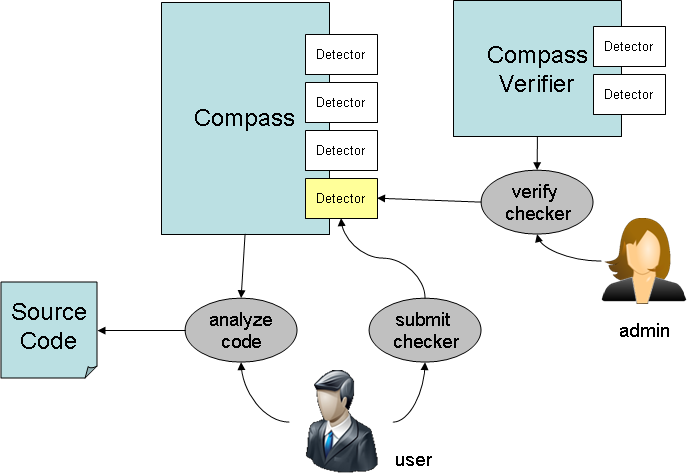
\includegraphics[width=4.5in]{compass_pic.png}
\caption{Compass Use Case}
\label{Compass_usecase}
\end{figure}

Furthermore, a user may contribute with his own detectors that he can add to Compass. Since 
external users may contribute detectors automatically via scripts, a verification of the 
validity and safety of these detectors is necessary. We provide a \emph{Compass Verifier}
that helps to check that all detectors are safe. Currently, the verifier is run by
a administrative person but may run automatically in the future.



\section{Design}

\begin{figure}[thb]
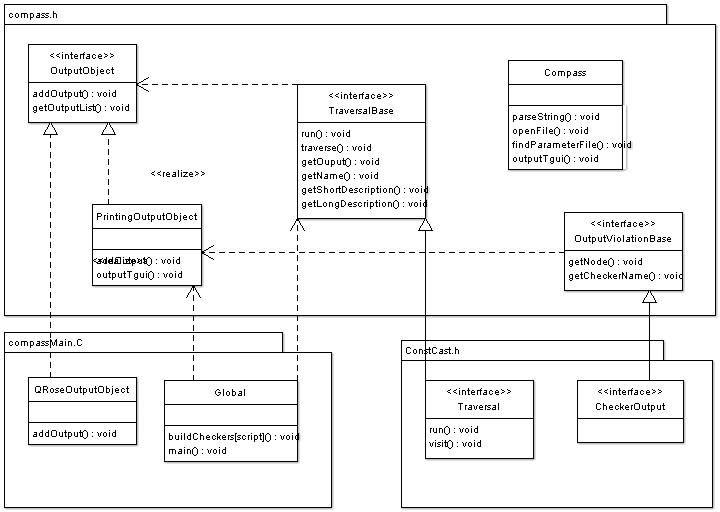
\includegraphics[width=6.0in]{compassdesign.png}
\caption{Compass Design}
\label{CompassDesign}
\end{figure}

Compass is designed to be easy to extend. Any user may write a detector and add it to Compass. Figure~\ref{CompassDesign}
illustrates the UML design decisions behind Compass.


Most of the functionality of Compass is in abstract classes hidden in the Compass namespace within compass.h - a file within
the compassSupport directory. All detectors, such as ConstCast illustrated in the figure, utilize the abstract classes
to traverse a program with all its nodes and to output violations found in that code according to the local algorithm.

CompassMain is the main executable that initially calls ROSE to parse a program. Then \emph{buildCheckers} is called to
load all detectors that are specified within a configuration file. The configuration file allows users to turn on and off
specific detectors for their run-time analyses. However, the configuration file only permits detectors to be loaded that 
were part of Compass at compile-time.

The main interface file compass.h contains the abstract classes \emph{TraversalBase} and 
\emph{OutputObject}. TraversalBase is the interface to ROSE, allowing a detector to traverse the ROSE AST (program) and hence
perform analysis on that AST. OutputObject aids to output defects found by a specific detector. More functionality to handle
e.g. file input and parameters provided to Compass, is provided within the Compass namespace.


\section{Compass Verifier}

\subsection{Threats} 

Compass must be safe, so that analyses and their results can be trusted. 
The main threats to the validity of Compass are:

\begin{itemize}
\item \emph{Malicious User}. A malicious user is an external user of Compass contributing a detector that performs malicious behaviour.  
\item \emph{Malicious Detector}. Compass is extensible and new detectos can be added externally (users outside the main development group).
  A detector can be programmed arbitrarily using the C/C++ and assembly programming languages. 
  It is therefore possible for a skilled programmer to hide malicious operations within a detector, e.g. allow a detector to scan the host machine and
  send data away. Compass must prevent detectors with malicious behaviour to be part of the Compass system. 
\item \emph{Source Code Replacement}. It should not be possible for users to exchange the source code of detectors within a running system,
  i.e. Compass cannot implement dynamic loading of detectors. Such a feature would compromise its safety.
\item \emph{Binary Replacement}. Another threat is the replacement of a valid Compass detector with a modified malicious version within a binary release of Compass.
  Therefore, Compass should be aware if parts of itself were modified and should not execute.
\end{itemize} 

\subsection{Safety Handling}

Compass is designed to be safe. The Compass Verifier is a stable separate copy of Compass that contains only a few detectors
to check (external and internal) user delivered detectors for safety. We have designed Compass in a way that it addresses the threats mentioned above:

\begin{itemize}
\item \emph{Malicious User}. Initially, we permit only trusted individuals to add new detectors to Compass. Once the verification process
  is matured, we will extend this policy to allow arbitrary users to contribute to Compass. 

\item \emph{Malicious Detector}. To prevent Compass to execute malicious code, the Compass Verifier executes its own detectors on
any user defined detector that is beeing considered to be added to Compass.
Currently, the Compass Verifier contains three detectors:

\begin{itemize}
\item \emph{fileReadOnlyAccess} ensures that a user defined detector perorms no write or execute operations on files. 
\item \emph{forbiddenFunctions} is a white list of function calls permitted in a detector. This list contains functions
that are trusted and hence considered unharmful when integrated to Compass.
\item \emph{noAsmStmtsOps} searches for assembly instructions in a detector and flags those as unsafe.
\end{itemize}

\item \emph{Source Code Replacement}. Detectors can only be added at compile time to Compass, not at run-time.
This means that detectors (meaning the source code) cannot be exchanged against unsafe versions at run-time. Furthermore, we allow only 
the Compass tool builder (admin) to build versions of Compass that must pass the Compass Verifier.

\item \emph{Binary Replacement}. Our goal is to perform a MD5 checksum on all the detectors part of the binary Compass distribution before
  Compass is executed. In this way Compass will not run if parts of it were modified.
\end{itemize} 


%The above list contains an important subset of detectors that enforce Compass detectors to be safe. 
%Additional detectors can easily be added to that list.
%In the future, a detector submitted to Compass, should go first through the automatic verifier, before it is either 
%added to Compass or denied.  



\chapter{Getting Started}

\label{gettingStarted:gettingStarted}

% \section{Building ROSE}

%  Purpose:
% \begin{itemize}
%    \item A. What you need to get started
%    \item B. Preparing the working copy
% \end{itemize}
% \begin{center}
% *********************  \newline
% \end{center}
% \vspace{0.25in}

   This chapter details how to build ROSE and how to begin to use ROSE to build a 
source-to-source translator.
ROSE uses EDG and SAGE III internally. EDG is a commercial (and proprietary) C++
frontend that we are permitted to use to support our research work. SAGE III is
loosely derived from SAGE II, which is derived from SAGE++.  SAGE III is a rewrite of 
SAGE II and uses a similar object-oriented design and a similar interface (API).
% We have made substantial changes in the development of Sage III, 
The developers of SAGE II suggested that we call our work on the C++
intermediate representation Sage III. We are thankful to the developers
of SAGE II for their work.
% It contains the software and hardware requirements of ROSE.
% Additionally, it details the installation of the software.

\section{ROSE Documentation and Where to Find It}

To simplify user access to the ROSE documentation, the pre-built postscript files are 
included in the {\tt ROSE/docs/Rose} directory of each ROSE distribution. These versions
are always kept up-to-date by the automated build system that generates
ROSE distributions:
% Documentation there is:
\begin{itemize}
   \item {\bf ROSE Web Page} : The ROSE Web page is located at
           \htmladdnormallink{www.roseCompiler.org}{http://www.roseCompiler.org}. \\
           The web page contains the ROSE manual, tutorial and developer API. 
           The API provides details about IR nodes and their usage (interfaces). The documentation
           is generated by Doxygen.
   \item {\bf ROSE offline Web content} : ROSE/docs/Rose/ROSE-\VersionNumber-HTML-Docs.ps.gz \\
       ROSE HTML documentation that is available without internet access.
   \item {\bf MANUAL} : ROSE/docs/Rose/ROSE-\VersionNumber-UserManual.ps.gz \\
       This is the ROSE User Manual which explains basic concepts about and capabilities within ROSE. \\
   \item {\bf TUTORIAL} : ROSE/docs/Rose/Tutorial/ROSE-\VersionNumber-Tutorial.tar.gz \\
       This is the ROSE Tutorial with numerous examples of how to use ROSE. \\
       The tutorial documentation is
           constructed using the following steps:
           \begin{enumerate}
              \item Actual source code for each example translator in the ROSE/tutorial
                    directory is included. 
              \item Each example is compiled.
              \item Inputs to the examples are taken from the ROSE/tutorial directory.
              \item Output generated from running each example is placed into the tutorial
                    documentation.
           \end{enumerate}
           Thus, the {\tt ROSE/tutorial} contains exact examples, and each
           example may be manipulated (changing either the example translators or the
           inputs to the examples).
   \item {\bf PAPERS} : ROSE/ROSE\_RESEARCH\_PAPERS.tar.gz \\
       These are the current ROSE related research papers.
\end{itemize}

\commentout{
   There are three forms of ROSE documentation, and a ROSE Web site and email list:
\begin{enumerate}
     \item ROSE User Manual \\
           The User Manual presents how to get started with ROSE and documents 
           features of the ROSE infrastructure.  The User Manual is found in 
           {\tt ROSE/docs/Rose} directory, or at the following web pages: \\
           \htmladdnormallink{ROSE User Manual (postscript version, relative link)}{http://www.rosecompiler.org/ROSE_UserManual/ROSE-0.9.5a-UserManual.ps}
           or \\
           \htmladdnormallink{ROSE User Manual (HTML version, relative link)}{http://www.rosecompiler.org/ROSE_UserManual/manual.html}
     \item ROSE Tutorial \\
           The ROSE Tutorial presents examples of how to use ROSE (found
           in the {\tt ROSE/tutorial} directory).  The ROSE Tutorial documentation is found in 
           {\tt ROSE/docs/Rose/Tutorial} directory and the tutorial documentation is
           constructed using the following steps:
           \begin{enumerate}
              \item Actual source code for each example translator in the ROSE/tutorial
                    directory is included. % into the tutorial documentation
              \item Each example is compiled.
              \item Inputs to the examples are taken from the ROSE/tutorial directory.
              \item Output generated from running each example is placed into the tutorial
                    documentation.
           \end{enumerate}
           Thus, the {\tt ROSE/tutorial} contains exact examples, and each
           example may be manipulated (changing either the example translators or the
           inputs to the examples).  The ROSE Tutorial can also be found at (link back 
           to LaTeX document): \\
           \htmladdnormallink{ROSE Tutorial (postscript version, relative link)}{http://www.rosecompiler.org/ROSE_Tutorial/ROSE-0.9.5a-Tutorial.ps}
           or \\
           \htmladdnormallink{ROSE Tutorial (html version, relative link)}{http://www.rosecompiler.org/ROSE_Tutorial/tutorial.html}
     \item ROSE HTML Reference: Intermediate Representation (IR) documentation \\
           This Web documentation gives the detail interfaces for each IR nodes
           (documentation generated by Doxygen).
           The HTML IR documentation is found in ROSE/docs/Rose directory 
           (available as HTML only): \\
           \htmladdnormallink{ROSE HTML Reference (relative
               link)}{http://www.rosecompiler.org/ROSE_HTML_Reference/index.html}
     \item ROSE Web Site \\
           The ROSE project maintains a Web site where this documentation and some
           additional information (including the ROSE software distribution:
           {\em starting late Summer 2006}) is available at
           \htmladdnormallink{ROSE Web Site
             (www.rosecompiler.org)}{http://www.rosecompiler.org}
     \item ROSE Email List \\
           The ROSE project maintains a mailing list (rose-public *at* nersc *dot* gov).
           Anyone who would like to be on the email list can subscribe to
           it at:
           \htmladdnormallink{ROSE Public Email List}
                {https://mailman.nersc.gov/mailman/listinfo/rose-public}.
\end{enumerate}
}

% DQ (1/20/2009): Fixing the reference to the email list for ROSE.
The ROSE project maintains an external mailing list (see information at:
\htmladdnormallink{www.roseCompiler.org}{http://www.roseCompiler.org} and click on the
{\bf Mailing Lists} link for how to join).

\input{installRose}


\section{Building Translators Using ROSE}

   At this point you should have installed ROSE. For examples of ROSE translators
see the ROSE-\VersionNumber-Tutorial.tar.gz and the examples in the {\tt ROSE/tutorial} 
directory.

\section{Robustness of ROSE}
    A significant focus of the ROSE project is on the robustness of
the software supporting our project.  We have based the C and C++ support
upon the use of the EDG frontend (the same commercial quality frontend used by most
commercial C++ compilers). ROSE is a research project at a Department or Energy (DOE)
national laboratory.  As such, it must handle DOE laboratory applications that
scale to a million lines of code or more.  ROSE is not an academic research
project, nor is it a commercial product.  This section will layout what we do to test 
ROSE, what parts we consider to be {\em robust}, and exactly what we mean by 
{\em robust}.

\subsection{How We Test ROSE}

\subsubsection{ROSE Regression Tests}
   Our regression test of collected bugs reported over several years
helps prevent the reintroduction of old bugs during the development process.
Additional test codes and applications codes help provide more complete
testing of ROSE. 

\subsubsection{Elsa Regression Tests}
   Recent work has included the a separate regression test suit from the Elsa
project (an open source C++ parser project).  This is tested infrequently at
this point, but will be folded into standard ROSE regression tests in the future.
We wish to thanks Scott McPeak for the use of his rather large collection of
tests that he uses within Elsa (about 1000 test codes that test many corners of
the C, C99, and C++ language).

\commentout{
\subsubsection{Application Codes}
   ROSE will be released after tests are complete on approximately 10 separate 
one-million-line application codes:
\begin{enumerate}
%  \item KULL \\
%         This is an important application at LLNL.
%  \item ALE3D \\
%         This is an important application at LLNL.
%  \item ARES \\
%         This is an important application at LLNL.
%  \item CHOMBO \\
%         This is an Adaptive Mesh Refinement (AMR) library at Lawrence Berkeley National Laboratory.
%  \item DiffPack \\
%         This is a numerical library originally developed at University of Oslo, Norway.
%         The developers have been substantial collaborators to the ROSE project.
   \item ROSE \\
          The compilation of compiler project (ROSE) with itself is a milestone 
          for any compiler project.  ROSE can be used to compile the ROSE source
          code and has provided a good test of the internal compiler robustness.
   \item Overture \\
          This is an internal DOE library that supports Overset Grid applications.
          It is well in excess of one million lines of code. It includes 
          the A++/P++ library and other libraries upon which it depends.
%  \item CHROMA \\
%         This is an Molecular Dynamics application developed at University of Illinois at
%   Urbana-Champaign (UIUC). This is not really a one million line code, I think, but 
%   Overture more than makes up the difference.
\end{enumerate}

The first six are mostly done, in the sense that there are about 10 bugs
that have been isolated which appear to be the only remaining
problems.  I am working on these bugs, but some are non-trivial (read {\em hard}).
}

\subsubsection{Plum Hall C and C++ Compiler Test Suite}
   This is a commercial C and C++ compiler test suit that was purchased
for us by the DOE Advanced Simulation and Computing (ASC) program.  We appreciate their 
substantial support of ROSE. They also fund part of the ROSE project, but these
test codes are REALLY hard.

\subsubsection{Nightly cron jobs}
Nightly regression tests are run on ROSE, these are easy to setup using the command 
{\tt crontab -e}, this will bring up an editor, then put in the following lines: 
\begin{verbatim}
# Time Spec, 1st column: minute, 2nd column: hours, 3rd column: day, 4th column: month, 5th column: year?; 
# then followed by the command to be run at the time specified by the time spec:
55 12 * * * cd /home/dquinlan/ROSE/svn-rose/scripts && ./roseFreshTest ./roseFreshTestStub-xyz.sh 
\end{verbatim}

Then build a special roseFreshTestStub-xyz.sh file (examples are in the {\em ROSE/scripts} 
directory); it holds the required paths for the environment to be setup.

%\fixme{What does the TID reference to "em-dash" mean.}

\subsection{What Parts of ROSE Are Robust}
    We consider the compiler construction issues -- IR, code generation, AST 
traversal support, and low level AST transformation mechanisms -- to be robust.  
These are the mechanisms that are dominantly tested by the regression suits 
and application codes.  Specifically, a ROSE translator is built that does no
transformation (e.g. {\em IdentityTransformation.C} in the ROSE Tutorial).
Input files are processed with this translator, and the following steps
are tested for each source file:
\begin{itemize}
   \item EDG's AST is built internally.
   \item ROSE's AST (the SAGE III AST) is built from the EDG AST.
   \item EDG's AST is deleted.
   \item ROSE's AST traversals are tested.
   \item ROSE's AST Attribute Mechanism is tested in each IR node.
   \item ROSE's AST internal tests are done (all tests must pass).
   \item ROSE's Code Generator is used to regenerate the source code.
   \item Vendor compiler compiles the ROSE-generated source code.
\end{itemize}

Note that separate tests to run the executables generated form the vendor compiler's
compilation of the ROSE generated sources are not automated.  This is not yet a
standard test in ROSE, just verified infrequently.

\subsection{What Parts of ROSE Are {\em Not} Robust}
    Basically, the program analysis lags in robustness. The robustness of the program analysis and 
optimization in ROSE has only recently become a focus.
This work is not yet as durable as the compiler construction aspects of ROSE.
The development of the ROSE infrastructure requires that we can first compile
and transform large scale applications before we address complex program analysis
and its robustness.

\section{Submitting a Bug Report}
     The rule is simple: the better quality the bug report, the higher priority it
gets.  All good bug reports include a very simple example that demonstrates
the bug, and only that bug, so that it is clearly reproducible.  We welcome your submission
of good quality bug reports.  You may also send email directly to 
{\it dquinlan *at* llnl *dot* gov}.  Any bug report you submit will be added as a test 
code and used to test future versions of ROSE (please add {\bf ROSE bug report} to the 
subject line).  At a later point we will use a more formal bug tracking mechanism.


\section{Getting a Free EDG License for Research Use}

ROSE source code is released under BSD license to make it as easy as possible to use.
ROSE uses the EDG (www.edg.com) C++ front-end to parse C++ code internally.
No part of the EDG source code is visible to the user or ROSE. ROSE distributes
a binary version of the EDG work for a limited but growing range of platforms (32-bit and 
64-bit Linux, Mac OSX, etc.). Since ROSE does not yet routinely package a separate binary 
for more than this range of platforms, we can optionally provide the EDG source code as 
part of the distribution of ROSE.  However, we only give out ROSE source code that 
includes the EDG source code to research groups that also get a free research license 
for the EDG source code (available from EDG).  

   We are particularly thankful to the EDG people for providing such a
good quality C++ front-end and for allowing it to be used for research work 
in C++.  They have permitted research work specific to the C++ language
to address the complexity of real application written in C++, which would not 
otherwise be practical or within the scope of a research project.

   To get a version of ROSE, we encourage you to contact EDG to obtain their research
license.  Instructions for getting an EDG license:

\begin{itemize}
     \item Send email to these three fellows at EDG:
     \begin{itemize}
          \item Steve Adamczyk       jsa at edg.com
          \item John Spicer          jhs at edg.com
          \item Daveed Vandevoorde   daveed at edg.com
     \end{itemize}
\end{itemize}

I suggest sending the email to all of them at the same time so that they can see that you have
sent email to the other two, since I really don't know which one is the correct person
to contact.  At some point we might get more information about a better approach.

The content of the email can be something like: \\
\begin{itemize}
   \item We would like to work with the ROSE project at Lawrence Livermore 
         National Laboratory (LLNL) which is using the EDG front-end for 
         research on C++ optimization. They have asked that we obtain a 
         research license in order to use ROSE for our research work with them.
\end{itemize}

They will then contact you (by email) and give you the location of the license form
to fill out and get signed.  They will either let you know where to
get the EDG software or suggest that you get our version of their code
directly from us.  We will then give you all of ROSE, which includes (at present)
the source code to the EDG front-end.  You will not need a version of EDG 
directly from them.














% Liao, 9/17/2009, Out of date information. We have better text in the
% developer guide now.
%\chapter{Making your Contributions to ROSE}

To make the process of contributing to ROSE go more smoothly, the following procedure has
been established.  Steps 1-3 should be followed for contributions of new code, and
step 2 for changes to existing code.

\begin{enumerate}
\item First of all, work outside of the ROSE tree.  You can use your own Makefile to control the build process.  An example of such a Makefile is shown in Figure~\ref{Tutorial:exampleMakefile} .

\item If you find you need to make changes to ROSE, make them directly to the ROSE source tree, and contribute patches as you work.  If you have access to the CVS repository, use the `\verb|cvs diff|' command to create patches.  If you are starting with a heavily patched version of ROSE, or don't have access to CVS, make a pristine copy of ROSE before you start and use the plain `\verb|diff|' command.

In order to meet the standard for ROSE patches, which include:
\begin{itemize}
\item Context information
\item Omission of machine-generated files
\end{itemize}
please supply the following flags to your `\verb|diff|' or `\verb|cvs diff|' command:

\begin{verbatim}
-u --exclude 'aclocal.m4' --exclude 'autom4te.cache' --exclude 'Makefile.in'
--exclude 'configure'
\end{verbatim}

If using `\verb|diff|' rather than `\verb|cvs diff|', the `\verb|-r|' flag is also required.

The syntax for the \verb|diff| command is as follows:

\begin{verbatim}
diff [flags] <dir1> <dir2> > <patchfile>
\end{verbatim}

For our purposes, the \verb|diff| command should be issued in the directory directly above the ROSE source directory.  Be sure to give the patch file a suitable name such as \verb|enhanced-template-support.patch|.  \verb|<dir1>| should be the name of your pristine source directory; \verb|<dir2>| that of your modified sources.  For example, if your pristine source tree is located at \verb|/home/me/research/ROSE-orig| and your modified sources are in \verb|/home/me/research/ROSE|, you can issue the commands:

\begin{verbatim}
$ cd /home/me/research
$ diff -ur --exclude 'aclocal.m4' --exclude 'autom4te.cache' --exclude 'Makefile.in'
  --exclude 'configure' ROSE-orig ROSE > my-changes.patch
\end{verbatim}

The syntax for the \verb|cvs diff| command is as follows:

\begin{verbatim}
cvs diff [flags] <dir> > <patchfile>
\end{verbatim}

This command should be given in the directory directly above that to which you wish to contribute changes.  Then the \verb|<dir>| option shall be the name of this directory.  For example, to create a patch for the \verb|src/frontend| directory, issue the following commands:

\begin{verbatim}
$ cd src
$ cvs diff -u --exclude 'aclocal.m4' --exclude 'autom4te.cache' --exclude 'Makefile.in'
  --exclude 'configure' frontend > my-changes.patch
\end{verbatim}

You will need to supply information to the maintainer on how to apply your patch.  You will need to look at the paths following the `\verb|---|' and `\verb|+++|' markers in the patch file.  If you used `\verb|cvs diff|' to create the patch, the paths will likely be relative to the directory you were in when you created the patch, and you'll need to apply the patch with `\verb|patch -p0|' in the same directory.  If you used `\verb|diff|' the path will probably include the name of your source tree root directory, and you'll need to use `\verb|patch -p1|' in the root of the source tree.

\item When you are ready to contribute the work, it should first be integrated into the ROSE tree.  Create a new directory either under \verb|projects| or a subdirectory of \verb|src|.  If you are unsure where to create your directory, contact the maintainer.  Once you have created the directory copy your files there, excluding the Makefile.

You will need to create a Makefile.am which integrates with the ROSE build process.  The best way to learn about these is by looking at other Makefile.am files in sibling directories to yours.  Note the differences between a `\verb|project|' and a `\verb|src|' Makefile.am, e.g. only the latter will create shared libraries.  Remember to add your new directory to the \verb|SUBDIRS| list in the parent directory's Makefile.am, and your Makefile.am to the list of Makefiles in \verb|configure.in| in the root directory.

If your project is in \verb|src|, your test cases should go into a subdirectory of \verb|tests/nonsmoke/functional/roseTests|, which mirrors the \verb|src| directory structure.  Otherwise they can go into your project directory.  Again, look at other Makefiles for information on how test cases work.

While making these changes, keep track of all the new files you create within the ROSE tree.  These will typically be all the files in your new directory as well as your test codes and test input codes in the \verb|tests| directory, if applicable.  Once you are done, `\verb|tar|' up all these files and send them to the maintainer, along with patches to existing files, created using `\verb|diff|' or `\verb|cvs diff|' as described in step 2.
\end{enumerate}

The current maintainer is Dan Quinlan \verb|<dquinlan@llnl.gov>|.

% Present the Makefile which will compile everything.

\chapter{Required Makefile for Tutorial Examples}
\label{TutorialMakefiles}

\fixme{The exampleMakefile needs to be modified to include the support for compiling
       all of the tutorial examples.}

    This section shows an example makefile~\ref{Tutorial:exampleMakefile} 
required for the compilation of many of the tutorial example programs 
using the installed libraries (assumed to be generated from {\tt make install}).
The build process can be tested by running {\tt make installcheck} from within 
the ROSE compile tree.  This {\tt makefile} can be found in the compile tree
{\em (not the source tree)} for ROSE in the {\tt tutorial} directory.

\begin{figure}[!h]
{\indent
{\mySmallFontSize

% Do this when processing latex to generate non-html (not using latex2html)
\begin{latexonly}
%  \lstinputlisting{\TutorialExampleBuildDirectory/exampleMakefile}
%  \verbatiminput{\TutorialExampleBuildDirectory/exampleMakefile}
   \listinginput{1}{\TutorialExampleBuildDirectory/exampleMakefile}
\end{latexonly}

% Do this when processing latex to build html (using latex2html)
\begin{htmlonly}
   \verbatiminput{\TutorialExampleBuildDirectory/exampleMakefile}
\end{htmlonly}

% end of scope in font size
}
% End of scope in indentation
}
% \caption{Example {\tt Makefile} .}
\caption{Example {\tt Makefile} showing how to use an installed version of ROSE (generated by {\tt make install}).}
\label{Tutorial:exampleMakefile}
\end{figure}



%-----------------------------------------------------------
%          Working with ROSE AST 
%-----------------------------------------------------------
\part[Working with the ROSE AST]{  Working with the ROSE AST \\
\vspace{1.0in}
\normalsize{Getting familiar with the ROSE AST is the basis for any advanced
usage of ROSE. This part of tutorial collects examples for AST
visualization, traversal, query, and debugging.}
}
%\part[Stable Parts of ROSE]{  Stable Parts of ROSE \\
%\vspace{1.0in}
%\normalsize{These parts of ROSE are tested regularly on large scale applications and are
%    suitable for use on ROSE projects requiring the greatest levels of robustness.}
%\fixme{Lay out rules and criteria for the classification of different parts of ROSE.}
%}

\chapter{Identity Translator}

  Using the input code in Figure~\ref{Tutorial:exampleInputCode_IdentityTranslator}
we now show a translator which builds the AST, generates the source code from the AST, 
and compiles the generated code using the backend vendor compiler\footnote{
Note: that the backend vendor compiler is selected at configuration time.}.
Figure~\ref{Tutorial:exampleIdentityTranslator} shows the source code for this
translator, the construction of the AST is identical to the previous code, but
we make an explicit call to the ROSE {\tt backend()} function.

\begin{figure}[!h]
{\indent
{\mySmallFontSize


% Do this when processing latex to generate non-html (not using latex2html)
\begin{latexonly}
   \lstinputlisting{\TutorialExampleDirectory/identityTranslator.C}
\end{latexonly}

% Do this when processing latex to build html (using latex2html)
\begin{htmlonly}
   \verbatiminput{\TutorialExampleDirectory/identityTranslator.C}
\end{htmlonly}

% end of scope in font size
}
% End of scope in indentation
}
\caption{Source code for translator to read an input program 
         and generate an object code (with no translation).}
\label{Tutorial:exampleIdentityTranslator}
\end{figure}

\begin{figure}[!h]
{\indent
{\mySmallFontSize


% Do this when processing latex to generate non-html (not using latex2html)
\begin{latexonly}
   \lstinputlisting{\TutorialExampleDirectory/inputCode_IdentityTranslator.C}
\end{latexonly}

% Do this when processing latex to build html (using latex2html)
\begin{htmlonly}
   \verbatiminput{\TutorialExampleDirectory/inputCode_IdentityTranslator.C}
\end{htmlonly}

% end of scope in font size
}
% End of scope in indentation
}
\caption{Example source code used as input to identity translator.}
\label{Tutorial:exampleInputCode_IdentityTranslator}
\end{figure}

Figure~\ref{Tutorial:exampleOutputFromTranslator} shows the generated code from the
processing of the {\tt identityTranslator} build using ROSE and using the input file
shown in figure~\ref{Tutorial:exampleInputCode_IdentityTranslator}.
This example also shows that the output generated from and ROSE translator is
a close reproduction of the input; preserving all comments, preprocessor
control structure, and most formating.  Note that all macros are expanded in
the generated code.

\begin{figure}[!h]
{\indent
{\mySmallFontSize


% Do this when processing latex to generate non-html (not using latex2html)
\begin{latexonly}
   \lstinputlisting{\TutorialExampleBuildDirectory/rose_inputCode_IdentityTranslator.C}
\end{latexonly}

% Do this when processing latex to build html (using latex2html)
\begin{htmlonly}
   \verbatiminput{\TutorialExampleBuildDirectory/rose_inputCode_IdentityTranslator.C}
\end{htmlonly}

% end of scope in font size
}
% End of scope in indentation
}
\caption{Generated code, from ROSE identity translator, sent to the backend (vendor) compiler.}
\label{Tutorial:exampleOutputFromTranslator}
\end{figure}

  In this trivial case of a program in a single file, the translator
compiles the application to build an executable (since {\tt -c}
was not specified on the command-line.





\chapter{AST Graph Generator}
\label{Tutorial:chapterASTGraphGenerator}

\paragraph{What To Learn From This Example}
This example shows how to generate and visualize the AST from any input program.
Each node of the graph in figure~\ref{tutorial:exampleOutputCodeGraph} shows
a node of the Intermediate Representation (IR).  Each edge shows the connection
of the IR nodes in memory. The generated graph shows the connection of different 
IR nodes to form the AST.  The generation of such graphs is appropriate for small 
input programs, chapter~\ref{Tutorial:chapterASTPDFGenerator} shows a mechanism 
using PDF files that is more appropriate to larger programs (e.g. 100K lines of code).
More information about generation of specialized AST graphs can be found in 
\ref{Tutorial:chapterGeneralASTGraphGeneration} and custom graph generation in
\ref{Tutorial:chapterCustomGraphs}.

\begin{figure}[!h]
{\indent
{\mySmallFontSize


% Do this when processing latex to generate non-html (not using latex2html)
\begin{latexonly}
   \lstinputlisting{\TutorialExampleDirectory/ASTGraphGenerator.C}
\end{latexonly}

% Do this when processing latex to build html (using latex2html)
\begin{htmlonly}
   \verbatiminput{\TutorialExampleDirectory/ASTGraphGenerator.C}
\end{htmlonly}

% end of scope in font size
}
% End of scope in indentation
}
\caption{Example source code to read an input program and generate an AST graph.}
\label{Tutorial:exampleASTGraphGenerator}
\end{figure}

The program in figure~\ref{Tutorial:exampleASTGraphGenerator} calls 
an internal ROSE function that traverses the AST and generates 
an ASCII file in {\tt dot} format.
Figure~\ref{Tutorial:exampleInputCode_ASTGraphGenerator} shows an input
code which is processed to generate a graph of the AST, generating a 
{\tt dot} file.   The {\tt dot} file is then processed
using {\tt dot} to generate a postscript file~\ref{tutorial:exampleOutputCodeGraph}
(within the {\tt Makefile}).
Note that a similar utility program already exists within ROSE/exampleTranslators
(and includes a utility to output an alternative PDF representation 
(suitable for larger ASTs) as well).  Figure~\ref{tutorial:exampleOutputCodeGraph}
(\TutorialExampleBuildDirectory/test.ps) can be found in the compile 
tree (in the tutorial directory) and viewed directly using ghostview 
or any postscript viewer to see more detail.


\begin{figure}[!h]
{\indent
{\mySmallFontSize

% Do this when processing latex to generate non-html (not using latex2html)
\begin{latexonly}
   \lstinputlisting{\TutorialExampleDirectory/inputCode_ASTGraphGenerator.C}
\end{latexonly}

% Do this when processing latex to build html (using latex2html)
\begin{htmlonly}
   \verbatiminput{\TutorialExampleDirectory/inputCode_ASTGraphGenerator.C}
\end{htmlonly}

% end of scope in font size
}
% End of scope in indentation
}
\caption{Example source code used as input to generate the AST graph.}
\label{Tutorial:exampleInputCode_ASTGraphGenerator}
\end{figure}

\begin{figure}
%\centerline{\epsfig{file=\TutorialExampleBuildDirectory/inputCode_ASTGraphGenerator.ps,
%                    height=1.3\linewidth,width=1.0\linewidth,angle=0}}
\includegraphics[scale=0.75]{\TutorialExampleBuildDirectory/inputCode_ASTGraphGenerator}
\caption{AST representing the source code file: inputCode\_ASTGraphGenerator.C.}
\label{tutorial:exampleOutputCodeGraph}
\end{figure}

   Figure~\ref{tutorial:exampleOutputCodeGraph} displays the individual
C++ nodes in ROSE's intermediate representation (IR).  Each circle represents
a single IR node, the name of the C++ construct appears in the center of the
circle, with the edge numbers of the traversal on top and the number of
child nodes appearing below.  Internal processing to build the graph generates
unique values for each IR node, a pointer address, which is displays at the bottom
of each circle.  The IR nodes are connected for form a tree, and abstract syntax
tree (AST). Each IR node is a C++ class, see SAGE III reference for details,
the edges represent the values of data members in the class (pointers which connect
the IR nodes to other IR nodes).  The edges are labeled with the names of the 
data members in the classes representing the IR nodes.

\fixme{Use this first example as a chance to explain the use of the
       header files (config.h and rose.h) and the code to build the 
       SgProject object.}




\chapter{AST Whole Graph Generator}
\label{Tutorial:chapterASTWholeGraphGenerator}

\paragraph{What To Learn From This Example}
This example shows how to generate and visualize the AST from any input program.
This view of the AST includes all additional IR nodes and edges that form attributes to
the AST, as a result this graph is not a tree.  These graphs are more complex but
show significantly more detail about the AST and its additional edges and attributes.
Each node of the graph in figure~\ref{tutorial:exampleOutputCodeWholeGraph} shows
a node of the Intermediate Representation (IR).  Each edge shows the connection
of the IR nodes in memory. The generated graph shows the connection of different 
IR nodes to form the AST and its additional attributes (e.g types, modifiers, etc).  
The generation of such graphs is appropriate for very small 
input programs, chapter~\ref{Tutorial:chapterASTPDFGenerator} shows a mechanism 
using PDF files that is more appropriate to larger programs (e.g. 100K lines of code).
More information about generation of specialized AST graphs can be found in 
\ref{Tutorial:chapterGeneralASTGraphGeneration} and custom graph generation in
\ref{Tutorial:chapterCustomGraphs}.

   {\em Viewing these dot files is best done using:} {\bf zgrviewer} at 
{\tt http://zvtm.sourceforge.net/zgrviewer.html}.  This tool permits zooming
in and out and viewing isolated parts of even very large graphs. {\bf Zgrviewer} permits 
a more natural way of understanding the AST and its additioan IR nodes than the 
pdf file displayed in these pages.  The few lines of code used to generate the
graphs can be used on any input code to better understand how the AST represents
different languages and their constructs.

\begin{figure}[!h]
{\indent
{\mySmallFontSize

% Do this when processing latex to generate non-html (not using latex2html)
\begin{latexonly}
   \lstinputlisting{\TutorialExampleDirectory/wholeASTGraphGenerator.C}
\end{latexonly}

% Do this when processing latex to build html (using latex2html)
\begin{htmlonly}
   \verbatiminput{\TutorialExampleDirectory/wholeASTGraphGenerator.C}
\end{htmlonly}

% end of scope in font size
}
% End of scope in indentation
}
\caption{Example source code to read an input program and generate a {\em whole} AST graph.}
\label{Tutorial:exampleASTWholeGraphGenerator}
\end{figure}

The program in figure~\ref{Tutorial:exampleASTWholeGraphGenerator} calls 
an internal ROSE function that traverses the AST and generates 
an ASCII file in {\tt dot} format.
Figure~\ref{Tutorial:exampleInputCode_ASTWholeGraphGenerator_small} shows an tiny input
code which is processed to generate a graph of the AST with its attributes, generating a 
{\tt dot} file.   The {\tt dot} file is then processed
using {\tt dot} to generate a pdf file~\ref{tutorial:exampleOutputCodeWholeGraph_small}
(within the {\tt Makefile}).
Note that a similar utility program already exists within ROSE/exampleTranslators
(and includes a utility to output an alternative PDF representation 
(suitable for larger ASTs) as well).  Figure~\ref{tutorial:exampleOutputCodeWholeGraph}
(\TutorialExampleBuildDirectory/test.ps) can be found in the compile 
tree (in the tutorial directory) and viewed directly using 
any pdf or dot viewer to see more detail ({\bf zgrviewer} working with
the dot file directly is strongly advised).

   Note that AST's can get very large, and that the additional IR nodes required to
represent the types, modifiers, etc, can generate visually complex graphs. ROSE
contains the mechanisms to traverse these graphs and do analysis on them.  In
one case the number of IR nodes exceeded 27 million, an analysis was done through
a traversal of the graph in 10 seconds on a desktop x86 machine (the memory requirements
were 6 Gig).  ROSE organizes the IR in ways that permit analysis of programs that can 
represent rather large ASTs.


% ************************************************************
%                     Small Graph Example
% ************************************************************

\begin{figure}[!h]
{\indent
{\mySmallFontSize

% Do this when processing latex to generate non-html (not using latex2html)
\begin{latexonly}
   \lstinputlisting{\TutorialExampleDirectory/inputCode_wholeAST_1.C}
\end{latexonly}

% Do this when processing latex to build html (using latex2html)
\begin{htmlonly}
   \verbatiminput{\TutorialExampleDirectory/inputCode_wholeAST_1.C}
\end{htmlonly}

% end of scope in font size
}
% End of scope in indentation
}
\caption{Example tiny source code used as input to generate the small AST graph with attributes.}
\label{Tutorial:exampleInputCode_ASTGraphGenerator_small}
\end{figure}

\begin{figure}
\includegraphics[scale=0.75]{\TutorialExampleBuildDirectory/inputCode_ASTWholeGraphGenerator_small}
\caption{AST representing the source code file: inputCode\_wholeAST\_1.C.}
\label{tutorial:exampleOutputCodeWholeGraph_small}
\end{figure}

   Figure~\ref{tutorial:exampleOutputCodeWholeGraph_small} displays the individual
C++ nodes in ROSE's intermediate representation (IR).  Colors and shapes are used to 
represent different types or IR nodes. Although only visible using {\bf zgrviewer} 
the name of the C++ construct appears in the center of each node in the graph, with 
the names of the data members in each IR node as edge labels. Unique pointer values
are includes and printed next to the IR node name.  These graphs are the single best
way to develop an intuitive understanding how language constructs are organized
in the AST.  In these graphs, the color yellow is used for types (SgType IR nodes),
the color green is used for expressions (SgExpression IR nodes), and statements
are a number of different colors and shapes to make them more recognizable.

% ************************************************************
%                     Large Graph Example
% ************************************************************

\begin{figure}[!h]
{\indent
{\mySmallFontSize

% Do this when processing latex to generate non-html (not using latex2html)
\begin{latexonly}
   \lstinputlisting{\TutorialExampleDirectory/inputCode_wholeAST_2.C}
\end{latexonly}

% Do this when processing latex to build html (using latex2html)
\begin{htmlonly}
   \verbatiminput{\TutorialExampleDirectory/inputCode_wholeAST_2.C}
\end{htmlonly}

% end of scope in font size
}
% End of scope in indentation
}
\caption{Example source code used as input to generate a larger AST graph with attributes.}
\label{Tutorial:exampleInputCode_ASTGraphGenerator_large}
\end{figure}

\begin{figure}
\includegraphics[scale=0.65]{\TutorialExampleBuildDirectory/inputCode_ASTWholeGraphGenerator_large}
\caption{AST representing the source code file: inputCode\_wholeAST\_2.C.}
\label{tutorial:exampleOutputCodeWholeGraph_large}
\end{figure}

   Figure~\ref{tutorial:exampleOutputCodeWholeGraph_large} shows a graph similar to the
previous graph but larger and more complex because it is from a larger code. Larger
graphs of this sort are still very useful in understanding how more significant
language constructs are organized and reference each other in the AST.  Tools
such as {\bf zgrviewer} are essential to reviewing and understanding these
graphs.


\chapter{General AST Graph Generation}
\label{Tutorial:chapterGeneralASTGraphGeneration}

\paragraph{What To Learn From This Example}
This example shows a maximally complete representation of the AST 
(often in more detail that is useful).

Where chapter~\ref{Tutorial:chapterASTGraphGenerator}
presented a ROSE-based translator which presented the AST as a tree, this chapter
presents the more general representation of the graph in which the AST is embedded.
The AST may be thought of as a subset of a more general graph or equivalently as
an AST (a tree in a formal sense) with annotations (extra edges and information),
sometimes referred to as a `{\em decorated} AST.

We present tools for seeing all the IR nodes in the graph containing the AST, including all types 
(SgType nodes), symbols (SgSymbol nodes), compiler generated IR nodes, and 
supporting IR nodes. In general
it is a specific filtering of this larger graph which is more useful to communicating
how the AST is designed and internally connected.  We use these graphs for internal 
debugging (typically on small problems where the graphs are reasonable in size).
The graphs presented using these graph mechanism present all back-edges, and
demonstrate what IR nodes are shared internally (typically SgType IR nodes).

First a few names, we will call the AST those nodes in the IR that are 
specified by a traversal using the ROSE traversal (SgSimpleTraversal, etc.).
We will call the graph of all IR nodes the {\em Graph of all IR nodes}.
the AST is embedded in the {\em Graph of all IR nodes}.  The AST {\em is} a tree,
while the {\em graph of all IR nodes} typically not a tree (in a Graph Theory sense)
since it typically contains cycles.

We cover the visualization of both the AST and the {\em Graph of all IR nodes}.
\begin{itemize}
   \item AST graph \\
   These techniques define ways of visualizing the AST and filtering IR nodes from being represented.
   \begin{itemize}
      \item Simple AST graphs
      \item Colored AST graphs
      \item Filtering the graph \\
      The AST graph may be generated for any subtree of the AST (not possible for the
    graphs of all IR nodes).  Additionally runtime options permit null pointers to be
    ignored. \fixme{Is this true?}.
   \end{itemize}
   \item {\em Graph of all IR nodes} \\
   These techniques define the ways of visualizing the whole graph of IR nodes and is
    based on the memory pool traversal as a means to access all IR nodes.  Even
    disconnected portions of the AST will be presented.
   \begin{itemize}
      \item Simple graphs
      \item Colored graphs
      \item Filtering the graph
   \end{itemize}
\end{itemize}


\section{Whole Graph Generation}

This example shows how to generate and visualize the AST from any input program.
Each node of the graph in figure~\ref{tutorial:exampleOutputWholeGraphAST} shows
a node of the Intermediate Representation (IR).  Each edge shows the connection
of the IR nodes in memory. The generated graph shows the connection of different 
IR nodes to form the AST.

\begin{figure}[!h]
{\indent
{\mySmallFontSize

% Do this when processing latex to generate non-html (not using latex2html)
\begin{latexonly}
   \lstinputlisting{\TutorialExampleDirectory/wholeGraphAST.C}
\end{latexonly}

% Do this when processing latex to build html (using latex2html)
\begin{htmlonly}
   \verbatiminput{\TutorialExampleDirectory/wholeGraphAST.C}
\end{htmlonly}

% end of scope in font size
}
% End of scope in indentation
}
\caption{Example source code to read an input program and generate an AST graph.}
\label{Tutorial:exampleWholeGraphAST}
\end{figure}

The program in figure~\ref{Tutorial:exampleWholeGraphAST} calls 
an internal ROSE function that traverses the AST and generates 
an ASCII file in {\tt dot} format.
Figure~\ref{Tutorial:exampleInputCode_WholeGraphAST} shows an input
code which is processed to generate a graph of the AST, generating a 
{\tt dot} file.   The {\tt dot} file is then processed
using {\tt dot} to generate a postscript file~\ref{tutorial:exampleOutputWholeGraphAST}
(within the {\tt Makefile}).
Note that a similar utility program already exists within ROSE/exampleTranslators
(and includes a utility to output an alternative PDF representation 
(suitable for larger ASTs) as well).  Figure~\ref{tutorial:exampleOutputWholeGraphAST}
(\TutorialExampleBuildDirectory/test.ps) can be found in the compile 
tree (in the tutorial directory) and viewed directly using ghostview 
or any postscript viewer to see more detail.


\begin{figure}[!h]
{\indent
{\mySmallFontSize

% Do this when processing latex to generate non-html (not using latex2html)
\begin{latexonly}
   \lstinputlisting{\TutorialExampleDirectory/inputCode_wholeGraphAST.C}
\end{latexonly}

% Do this when processing latex to build html (using latex2html)
\begin{htmlonly}
   \verbatiminput{\TutorialExampleDirectory/inputCode_wholeGraphAST.C}
\end{htmlonly}

% end of scope in font size
}
% End of scope in indentation
}
\caption{Example source code used as input to generate the AST graph.}
\label{Tutorial:exampleInputCode_WholeGraphAST}
\end{figure}

\begin{figure}
%\centerline{\epsfig{file=\TutorialExampleBuildDirectory/wholeGraphAST.ps,
%                    height=1.3\linewidth,width=1.0\linewidth,angle=0}}
\includegraphics[scale=0.5]{\TutorialExampleBuildDirectory/wholeGraphAST}
\caption{AST representing the source code file: inputCode\_wholeGraphAST.C.}
\label{tutorial:exampleOutputWholeGraphAST}
\end{figure}

   Figure~\ref{tutorial:exampleOutputWholeGraphAST} displays the individual
C++ nodes in ROSE's intermediate representation (IR).  Each circle represents
a single IR node, the name of the C++ construct appears in the center of the
circle, with the edge numbers of the traversal on top and the number of
child nodes appearing below.  Internal processing to build the graph generates
unique values for each IR node, a pointer address, which is displays at the bottom
of each circle.  The IR nodes are connected for form a tree, and abstract syntax
tree (AST). Each IR node is a C++ class, see SAGE III reference for details,
the edges represent the values of data members in the class (pointers which connect
the IR nodes to other IR nodes).  The edges are labeled with the names of the 
data members in the classes representing the IR nodes.



\chapter{AST PDF Generator}
\label{Tutorial:chapter_AST_PDF_Generator}

\paragraph{What To Learn From This Example}
This example demonstrates a mechanism for generating a visualization
of the AST using pdf files.  A pdf file is generated and can be viewed 
using {\tt acroread}.  The format is suitable for much larger input 
programs than the example shown in previous chapters using dot
format~\ref{Tutorial:chapterASTWholeGraphGenerator}.
This mechanism can support the visualization of input files around 100K 
lines of code.

\begin{figure}[!h]
{\indent
{\mySmallFontSize


% Do this when processing latex to generate non-html (not using latex2html)
\begin{latexonly}
   \lstinputlisting{\TutorialExampleDirectory/AST_PDF_Generator.C}
\end{latexonly}

% Do this when processing latex to build html (using latex2html)
\begin{htmlonly}
   \verbatiminput{\TutorialExampleDirectory/AST_PDF_Generator.C}
\end{htmlonly}

% end of scope in font size
}
% End of scope in indentation
}
\caption{Example source code to read an input program and generate a PDF file to represent the AST.}
\label{Tutorial:exampleAST_PDF_Generator}
\end{figure}

\begin{figure}[!h]
{\indent
{\mySmallFontSize


% Do this when processing latex to generate non-html (not using latex2html)
\begin{latexonly}
   \lstinputlisting{\TutorialExampleDirectory/inputCode_ASTGraphGenerator.C}
\end{latexonly}

% Do this when processing latex to build html (using latex2html)
\begin{htmlonly}
   \verbatiminput{\TutorialExampleDirectory/inputCode_ASTGraphGenerator.C}
\end{htmlonly}

% end of scope in font size
}
% End of scope in indentation
}
\caption{Example source code used as input to generate the PDF file of the AST.}
\label{Tutorial:exampleInputCode_AST_PDF_Generator}
\end{figure}

\begin{figure}
%\centerline{\epsfig{file=\TranslatorExampleDirectory/AST-pdf2.ps,height=0.75\linewidth,width=1.0\linewidth,angle=0}}
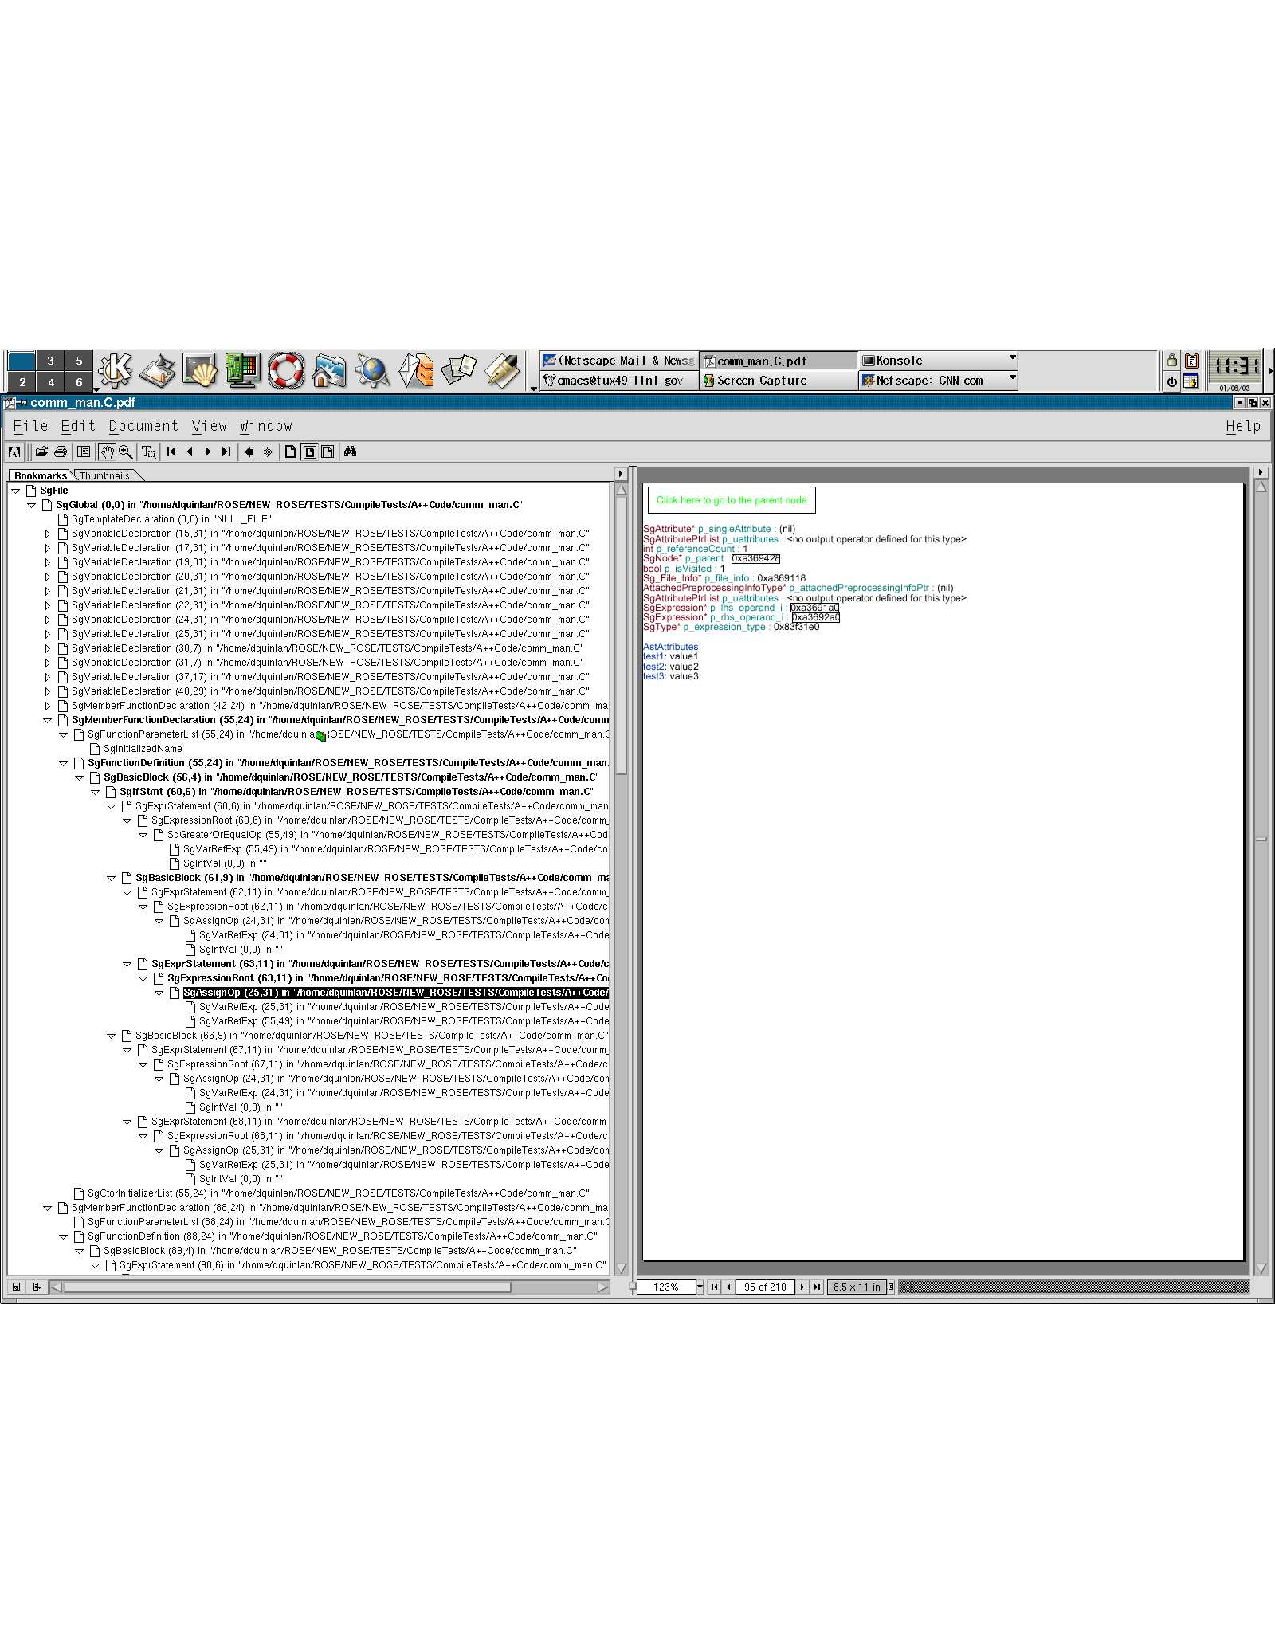
\includegraphics[scale=0.8]{\TranslatorExampleDirectory/AST-pdf2}
\caption{Example output from translator which outputs PDF representation of AST.}
\label{tutorial:exampleOutputCodePDF}
\end{figure}

The program in figure~\ref{Tutorial:exampleAST_PDF_Generator} calls 
an internal ROSE function that traverses the AST and generates 
an ASCI file in {\tt dot} format.
Figure~\ref{Tutorial:exampleInputCode_ASTGraphGenerator} shows an input
code which is processed to generate a graph of the AST, generating a 
{\tt pdf} file.   The {\tt pdf} file is then processed
using {\tt acroread} to generate a GUI for viewing the AST.

A standalone utility tool, called \textit{pdfGenerator} is provided within
ROSE. It is available from
\textit{ROSE\_BUILD/exampleTranslators/PDFGenerator} or
\textit{ROSE\_INS/bin}. Users can use it to generate AST in a pdf format
from an input code.

   Figure~\ref{tutorial:exampleOutputCodePDF} displays on the left hand side the individual
C++ nodes in ROSE's intermediate representation (IR).  The page on the right hand side
shows that IR nodes member data. Pointers in boxes can be clicked on to navigate the AST
(or nodes in the tree hierarchy can be clicked on jump to any location in the AST.
This representation shows only the IR nodes that are traversed by the standard traversal
(no SgSymbol or SgType IR nodes are presented in this view of the AST).

% Alternative description
The output of this translator is shown in figure \ref{tutorial:exampleOutputCodePDF}.  The left hand side
of the screen is a tree with click-able nodes to expand/collapse the subtrees.
The right hand side of the screen is a description of the data at a particular 
node in the AST (the node where the user has clicked the left mouse button).
This relatively simple view of the AST is useful for debugging transformation and finding
information in the AST required by specific sorts of analysis.  It is also useful
for developing an intuitive feel for what information is in the AST, how it is organized, 
and where it is stored.


\chapter{Introduction to AST Traversals}
\label{chap:traversals}

% Suggestions from discussions with Jim McGraw about this chapter.
\fixme{Add {\bf What to learn from this example} paragraph to each example.}
\fixme{Add {\bf What is different from previous example} paragraph to each example.}
\fixme{Add a table and/or graph at the end of this chapter to summarize the traversals.}

    An essential operation in the analysis and construction of ASTs is the
definition of traversals upon the AST to gather information and modify
targeted internal representation (IR) nodes.  ROSE includes different
sorts of traversals to address the different requirements of numerous
program analysis and transformation operations.  This section demonstrates
the different types of traversals that are possible using ROSE.

    ROSE translators most commonly introduce transformations and analysis
through a traversal over the AST.  Alternatives could be to generate
a simpler IR that is more suitable to a specific transformation and
either convert modification to that transformation specific IR
into changes to the AST or generate source code from the transformation specific
IR directly.  These approaches are more complex than introducing changes
to the AST directly, but may be better for specific transformations.

   Traversals represent an essential operation on the AST and there are a
number of different types of traversals.  The suggested traversals for users
are explained in Section~\ref{Tutorial:astStructureTraversals}.
Section~\ref{Tutorial:memoryPoolTraversals} introduces specialized traversals
(that traverse the AST in different orders and traverse types and symbols),
typically not appropriate for most translators (but perhaps appropriate for
specialized tools, often internal tools within ROSE).

See the ROSE User Manual for a more complete introduction to the different types of
traversals.  The purpose of this tutorial is to present examples, but we focus less on
the background and philosophy here than in the ROSE User Manual.

% GB (9/10/2007): I think these points are now taken care of.
%\fixme{Comments from Jacob:
%    1) Describe what the traversals are used for.
%    2) Reference ROSE User Manual.
%  }

   This chapter presents a number of ways of traversing the AST
of any input source code.  These {\em traversals} permit operations
on the AST, which may either read or modify the AST in place.  Modifications
to the AST will be reflected in the source code generated when the AST is 
{\em unparsed}; the code generation phase of the source-to-source process
defined by ROSE.  Note that for all examples, the input code described in 
section~\ref{Tutorial:exampleInputCodeDescription} is used to generate
all outputs shown with each translator.


\section{Input For Example Traversals}
\label{Tutorial:exampleInputCodeDescription}

\begin{figure}[!h]
{\indent
{\mySmallFontSize

% Do this when processing latex to generate non-html (not using latex2html)
\begin{latexonly}
   \lstinputlisting{\TutorialExampleDirectory/inputCode_ExampleTraversals.C}
\end{latexonly}

% Do this when processing latex to build html (using latex2html)
\begin{htmlonly}
   \verbatiminput{\TutorialExampleDirectory/inputCode_ExampleTraversals.C}
\end{htmlonly}

% end of scope in font size
}
% End of scope in indentation
}
\caption{Example source code used as input to program in
         traversals shown in this chapter.}
\label{Tutorial:exampleInputCode_ExampleTraversals}
\end{figure}

   The code shown in figure~\ref{Tutorial:exampleInputCode_ExampleTraversals}
shows the input code that will be used to demonstrate the traversals in this 
chapter.  It may be modified by the user to experiment with the use of the traversals
on alternative input codes.


%\clearpage
\section{Traversals of the AST Structure}
\label{Tutorial:astStructureTraversals}

    This collection of traversals operates on the AST in an order
which matches the structure of the AST and the associated source code.
These types of traversals are the most common traversals for users
to use.  A subsequent section of this chapter demonstrated more
specialized traversals over all IR nodes (more than just those IR nodes
in the AST representing the structure of the source code) that are 
suitable for some tools, mostly tools built internally within ROSE.

   Because the traversals in this section traverse the structure of
the source code (see the AST graph presented in the first tutorial 
example) they are more appropriate for most transformations
of the source code.  We suggest that the user focus on these 
traversals which represent the interface we promote for analysis
and transformation of the AST, instead of the memory pools traversals
which are suitable mostly for highly specialized internal tools.
The simple traversals of both kinds have the same interface so the user may
easily switch between them with out significant difficulty.

% \clearpage
% \subsection{Classic Object-Oriented Visitor Pattern for the AST (Not Yet Implemented)}
\subsection{Classic Object-Oriented Visitor Pattern for the AST}

   We show this example first, but it is rarely used in practice, and
more useful traversals follow.  It is however most closely similar to
traversals that are available in other compiler infrastructures, and so
a concept with which many people will be familar.  In this case because
this implementation is based on the memory pool infrstructure it will
visit all node and not in any order based on the AST.  The ASTSimpleProcessing
traversal in section~\ref{ASTSimpleProcessing_traversal} is closer to a common 
visitor pattern that visits the IR nodes in the order in which they appear in 
the AST.

\begin{figure}[!h]
{\indent
{\mySmallFontSize

% Do this when processing latex to generate non-html (not using latex2html)
\begin{latexonly}
   \lstinputlisting{\TutorialExampleDirectory/classicObjectOrientedVisitorPatternMemoryPoolTraversal.C}
\end{latexonly}

% Do this when processing latex to build html (using latex2html)
\begin{htmlonly}
   \verbatiminput{\TutorialExampleDirectory/classicObjectOrientedVisitorPatternMemoryPoolTraversal.C}
\end{htmlonly}

% end of scope in font size
}
% End of scope in indentation
}
\caption{Example source showing simple visitor pattern.}
\label{Tutorial:exampleClassicVisitorPattern}
\end{figure}


\begin{figure}[!h]
{\indent
{\mySmallFontSize


% Do this when processing latex to generate non-html (not using latex2html)
\begin{latexonly}
   \lstinputlisting{\TutorialExampleBuildDirectory/classicObjectOrientedVisitorPatternMemoryPoolTraversal.out}
\end{latexonly}

% Do this when processing latex to build html (using latex2html)
\begin{htmlonly}
   \verbatiminput{\TutorialExampleBuildDirectory/classicObjectOrientedVisitorPatternMemoryPoolTraversal.out}
\end{htmlonly}

% end of scope in font size
}
% End of scope in indentation
}
\caption{Output of input file to the visitor pattern traversal over the memory pools.}
\label{Tutorial:exampleOutput_ClassicVisitorPattern}
\end{figure}

Figure~\ref{Tutorial:exampleClassicVisitorPattern} shows the source code 
for a translator using the classic object-oriented visitor pattern 
to traverse the AST.  {\em This visitor pattern is only implemented
for the memory pool based traversal.}  Thus it works on the whole
of the attributed AST and does not work on a restricted subset of 
the AST (e.g. a subtree of the unattributed AST).
% It is however expected to appear identical to the classing visitor pattern 
% shown for the memory pool traversal.} 
Figure~\ref{Tutorial:exampleOutput_ClassicVisitorPattern} shows the 
output from this traversal using the example input source from 
figure~\ref{Tutorial:exampleInputCode_ExampleTraversals}.



% \clearpage
\subsection{Simple Traversal (no attributes)}
\label{ASTSimpleProcessing_traversal}

\begin{figure}[!h]
{\indent
{\mySmallFontSize

% Do this when processing latex to generate non-html (not using latex2html)
\begin{latexonly}
   \lstinputlisting{\TutorialExampleDirectory/visitorTraversal.C}
\end{latexonly}

% Do this when processing latex to build html (using latex2html)
\begin{htmlonly}
   \verbatiminput{\TutorialExampleDirectory/visitorTraversal.C}
\end{htmlonly}

% end of scope in font size
}
% End of scope in indentation
}
\caption{Example source showing simple visitor pattern.}
\label{Tutorial:exampleVisitorTraversal}
\end{figure}


\begin{figure}[!h]
{\indent
{\mySmallFontSize


% Do this when processing latex to generate non-html (not using latex2html)
\begin{latexonly}
   \lstinputlisting{\TutorialExampleBuildDirectory/visitorTraversal.out}
\end{latexonly}

% Do this when processing latex to build html (using latex2html)
\begin{htmlonly}
   \verbatiminput{\TutorialExampleBuildDirectory/visitorTraversal.out}
\end{htmlonly}

% end of scope in font size
}
% End of scope in indentation
}
\caption{Output of input file to the visitor traversal.}
\label{Tutorial:exampleOutput_VisitorTraversal}
\end{figure}

Figure~\ref{Tutorial:exampleVisitorTraversal} shows the source code 
for a translator which traverses the AST.  The traversal object is
from the type {\tt visitorTraversal} derived from {\tt AstSimpleProcessing}.
The {\tt visit()} function is required to be defined because it is 
defined as a pure virutal funciton in the {\tt AstSimpleProcessing} base class.
The member function {\tt traverseInputFiles()} of {\tt AstSimpleProcessing} 
is called to traverse the AST and call the {\tt visit()} function on each
IR node.  Note that the function {\tt traverse()} (not used) would visit
each IR nodes while {\tt traverseInputFiles()} will only visit those
IR nodes that originate in the input source code (thus skipping all 
header files).

For each node where the {\tt visit()} function is called a {\tt SgNode} 
pointer is to the node is passed into the {\tt visit} function.
% using only the input information represented by the current node.
Note that using this simple traversal
the only context information available to the visit function is what is stored
in its member variables (though access to other nodes is possible along
any edges in the attributed AST graph).
The only option is to traverse the AST in either pre-order or postorder.
The {\tt atTraversalEnd()} function may be defined by the user to do final
processing after all nodes have been visited (or to perform preparations
before the nodes are visited, in the case of the corresponding {\tt
atTraversalStart()} function).
Figure~\ref{Tutorial:exampleOutput_VisitorTraversal} shows the 
output from this traversal using the example input source from 
figure~\ref{Tutorial:exampleInputCode_ExampleTraversals}.

\subsection{Simple Pre- and Postorder Traversal}

\begin{figure}[!h]
{\indent
{\mySmallFontSize

% Do this when processing latex to generate non-html (not using latex2html)
\begin{latexonly}
   \lstinputlisting{\TutorialExampleDirectory/prePostTraversal.C}
\end{latexonly}

% Do this when processing latex to build html (using latex2html)
\begin{htmlonly}
   \verbatiminput{\TutorialExampleDirectory/prePostTraversal.C}
\end{htmlonly}

% end of scope in font size
}
% End of scope in indentation
}
\caption{Example source showing simple pre- and postorder pattern.}
\label{Tutorial:examplePrePostTraversal}
\end{figure}


\begin{figure}[!h]
{\indent
{\mySmallFontSize


% Do this when processing latex to generate non-html (not using latex2html)
\begin{latexonly}
   \lstinputlisting{\TutorialExampleBuildDirectory/prePostTraversal.out}
\end{latexonly}

% Do this when processing latex to build html (using latex2html)
\begin{htmlonly}
   \verbatiminput{\TutorialExampleBuildDirectory/prePostTraversal.out}
\end{htmlonly}

% end of scope in font size
}
% End of scope in indentation
}
\caption{Output of input file to the pre- and postorder traversal.}
\label{Tutorial:exampleOutput_PrePostTraversal}
\end{figure}

Figure~\ref{Tutorial:examplePrePostTraversal} shows the source code for a
translator that traverses the AST without attributes (like the one in the
previous subsection), but visiting each node twice, once in preorder (before
its children) and once in postorder (after all children).
Figure~\ref{Tutorial:exampleOutput_PrePostTraversal} shows the 
output from this traversal using the example input source from 
figure~\ref{Tutorial:exampleInputCode_ExampleTraversals}.


% \clearpage
\subsection{Inherited Attributes}

\begin{figure}[!h]
{\indent
{\mySmallFontSize


% Do this when processing latex to generate non-html (not using latex2html)
\begin{latexonly}
   \lstinputlisting{\TutorialExampleDirectory/inheritedAttributeTraversal.C}
\end{latexonly}

% Do this when processing latex to build html (using latex2html)
\begin{htmlonly}
   \verbatiminput{\TutorialExampleDirectory/inheritedAttributeTraversal.C}
\end{htmlonly}

% end of scope in font size
}
% End of scope in indentation
}
\caption{Example source code showing use of inherited attributes (passing context
         information {\bf down} the AST.}
\label{Tutorial:exampleInheritedAttributeTraversal}
\end{figure}

\begin{figure}[!h]
{\indent
{\mySmallFontSize


% Do this when processing latex to generate non-html (not using latex2html)
\begin{latexonly}
   \lstinputlisting{\TutorialExampleBuildDirectory/inheritedAttributeTraversal.out}
\end{latexonly}

% Do this when processing latex to build html (using latex2html)
\begin{htmlonly}
   \verbatiminput{\TutorialExampleBuildDirectory/inheritedAttributeTraversal.out}
\end{htmlonly}

% end of scope in font size
}
% End of scope in indentation
}
\caption{Output of input file to the inherited attribute traversal.}
\label{Tutorial:exampleOutput_InheritedAttributeTraversal}
\end{figure}

Figure~\ref{Tutorial:exampleInheritedAttributeTraversal} shows the use
of inherited attributes associated with each IR node.  Within this
traversal the attributes are managed by the traversal and exist on the
stack.  Thus the lifetime of the attributes is only as long as the
processing of the IR node and its subtree.  Attributes such as this
are used to communicate context information {\bf down} the AST and
called {\em Inherited attributes}.

In the example the class \verb+Inherited Attribute+ is used to represent 
inherited attribute. Each instance of the class represents an attribute 
value. When the AST is traversed we obtain as output the loop nest depth 
at each point in the AST. The output uses the example input source from 
figure~\ref{Tutorial:exampleInputCode_ExampleTraversals}.

Note that inherited attributes are passed by-value down the AST. In very rare
cases you might want to pass a pointer to dynamically allocated memory as an
inherited attribute. In this case you can define the virtual member function
{\tt void destroyInheritedValue(SgNode *n, InheritedAttribute inheritedValue)}
which is called after the last use of the inherited attribute computed at this
node, i.\,e.~after all children have been visited. You can use this function
to free the memory allocated for this inherited attribute.




\clearpage
\subsection{Synthesized Attributes}

\begin{figure}[!h]
{\indent
{\mySmallFontSize


% Do this when processing latex to generate non-html (not using latex2html)
\begin{latexonly}
   \lstinputlisting{\TutorialExampleDirectory/synthesizedAttributeTraversal.C}
\end{latexonly}

% Do this when processing latex to build html (using latex2html)
\begin{htmlonly}
   \verbatiminput{\TutorialExampleDirectory/synthesizedAttributeTraversal.C}
\end{htmlonly}

% end of scope in font size
}
% End of scope in indentation
}
\caption{Example source code showing use of synthesized attributed (passing analysis
         information {\bf up} the AST).}
\label{Tutorial:exampleSynthesizedAttributeTraversal}
\end{figure}

\begin{figure}[!h]
{\indent
{\mySmallFontSize


% Do this when processing latex to generate non-html (not using latex2html)
\begin{latexonly}
   \lstinputlisting{\TutorialExampleBuildDirectory/synthesizedAttributeTraversal.out}
\end{latexonly}

% Do this when processing latex to build html (using latex2html)
\begin{htmlonly}
   \verbatiminput{\TutorialExampleBuildDirectory/synthesizedAttributeTraversal.out}
\end{htmlonly}

% end of scope in font size
}
% End of scope in indentation
}
\caption{Output of input file to the synthesized attribute traversal.}
\label{Tutorial:exampleOutput_SynthesizedAttributeTraversal}
\end{figure}

  Figure~\ref{Tutorial:exampleSynthesizedAttributeTraversal} shows the use of
attributes to pass information {\bf up} the AST.  The lifetime of the attributes
are similar as for inherited attributes.  Attributes such as these are called
synthesized attributes.  

   This code shows the code for a translator which does an analysis of 
an input source code to determine the presence of loops.  It returns true if
a loop exists in the input code and false otherwise.  The list of synthesized
attributes representing the information passed up the AST from a node's
children is of type {\tt SynthesizedAttributesList}, which is a type that
behaves very similarly to {\tt vector<SynthesizedAttribute>} (it supports
iterators, can be indexed, and can be used with STL algorithms).

   The example determines the existence of loops for a given program.



\clearpage
\subsection{Accumulator Attributes}

\begin{figure}[!h]
{\indent
{\mySmallFontSize


% Do this when processing latex to generate non-html (not using latex2html)
\begin{latexonly}
   \lstinputlisting{\TutorialExampleDirectory/accumulatorAttributeTraversal.C}
\end{latexonly}

% Do this when processing latex to build html (using latex2html)
\begin{htmlonly}
   \verbatiminput{\TutorialExampleDirectory/accumulatorAttributeTraversal.C}
\end{htmlonly}

% end of scope in font size
}
% End of scope in indentation
}
\caption{Example source code showing use of accumulator attributes (typically to count
    things in the AST).}
\label{Tutorial:exampleAccumulatorAttributeTraversal}
\end{figure}


\begin{figure}[!h]
{\indent
{\mySmallFontSize


% Do this when processing latex to generate non-html (not using latex2html)
\begin{latexonly}
   \lstinputlisting{\TutorialExampleBuildDirectory/accumulatorAttributeTraversal.out}
\end{latexonly}

% Do this when processing latex to build html (using latex2html)
\begin{htmlonly}
   \verbatiminput{\TutorialExampleBuildDirectory/accumulatorAttributeTraversal.out}
\end{htmlonly}

% end of scope in font size
}
% End of scope in indentation
}
\caption{Output of input file to the accumulator attribute traversal.}
\label{Tutorial:exampleOutput_AccumulatorAttributeTraversal}
\end{figure}

   Figure~\ref{Tutorial:exampleAccumulatorAttributeTraversal} shows the use of
a different sort of attribute.  This attribute has a lifetime equal to the
lifetime of the traversal object (much longer than the traversal of any subset 
of IR nodes).  The same attribute is accessible from each IR node.  Such 
attributes are called {\em accumulator} attributes and are semantically 
equivalent to a global variable. Accumulator attributes
act as global variables which can easily be used to count application 
specific properties within the AST. 

Note that due to the limitation that the computation of inherited attributes cannot be made dependent on the values of synthesized attributes, counting operations cannot be implemented by combining these attributes as is usually done in attribute grammars. However, the use of accumulator attributes serves well for this purpose. Therefore all counting-like operations should be implemented using accumulator attributes (= member variables of traversal or processing classes).

     Although not shown in this tutorial explicitly, accumulator attributes
may be easily mixed with inherited and/or synthesized attributes.

In this example we count the number of for-loops in an input program.







% DQ (9/3/2006): We need an example of this for completeness.
% We can replace the current version with a newer version from 
% Markus when it is available.
% MS: commented out the following section because the implementation
% is not finished yet. Also, this case is covered by the new example
% loopNestingInfoProcessing which I've just added.
% GB (9/10/2007): Provided a simple example for this section.
% \commentout{
% \clearpage
\subsection{Inherited and Synthesized Attributes}

\begin{figure}[!h]
{\indent
{\mySmallestFontSize


% Do this when processing latex to generate non-html (not using latex2html)
\begin{latexonly}
   \lstinputlisting{\TutorialExampleDirectory/inheritedAndSynthesizedAttributeTraversal.C}
%  \lstinputlisting{\TutorialExampleBuildDirectory/inheritedAndSynthesizedAttributeTraversal.aa}
\end{latexonly}

% Do this when processing latex to build html (using latex2html)
\begin{htmlonly}
   \verbatiminput{\TutorialExampleDirectory/inheritedAndSynthesizedAttributeTraversal.C}
\end{htmlonly}

% end of scope in font size
}
% End of scope in indentation
}
\caption{Example source code showing use of both inherited and synthesized attributes
         working together (part 1).}
\label{Tutorial:exampleInheritedAndSynthesizedAttributeTraversal-part1}
\end{figure}

\commentout{
\begin{figure}[!h]
{\indent
{\mySmallestFontSize

% Do this when processing latex to generate non-html (not using latex2html)
\begin{latexonly}
   \lstinputlisting{\TutorialExampleBuildDirectory/inheritedAndSynthesizedAttributeTraversal.ab}
\end{latexonly}

% Do this when processing latex to build html (using latex2html)
\begin{htmlonly}
   \verbatiminput{\TutorialExampleDirectory/inheritedAndSynthesizedAttributeTraversal.C}
\end{htmlonly}

% end of scope in font size
}
% End of scope in indentation
}
\caption{Example source code showing the use of both inherited and synthesized attributes
         working together (part 2).}
\label{Tutorial:exampleInheritedAndSynthesizedAttributeTraversal-part2}
\end{figure}

% commented out
}

\begin{figure}[!h]
{\indent
{\mySmallFontSize

% Do this when processing latex to generate non-html (not using latex2html)
\begin{latexonly}
   \lstinputlisting{\TutorialExampleBuildDirectory/inheritedAndSynthesizedAttributeTraversal.out}
\end{latexonly}

% Do this when processing latex to build html (using latex2html)
\begin{htmlonly}
   \verbatiminput{\TutorialExampleBuildDirectory/inheritedAndSynthesizedAttributeTraversal.out}
\end{htmlonly}

% end of scope in font size
}
% End of scope in indentation
}
\caption{Output of input file to the inherited and synthesized attribute traversal.}
\label{Tutorial:exampleOutput_InheritedAndSynthesizedAttributeTraversal}
\end{figure}

   Figure~\ref{Tutorial:exampleInheritedAndSynthesizedAttributeTraversal-part1}
shows the combined use of inherited and synthesized attributes.  The example
source code shows the mixed use of such attributes to list the functions 
containing loop.  Inherited attributes are used to communicate that 
the traversal is in a function, which the synthesized attributes are
used to pass back the existence of loops deeper within the subtrees
associated with each function.

    List of functions containing loops.

% DQ (9/3/2006): uncommented by Dan.
% Commented out by Markus because it is not finished
% }






\clearpage
\subsection{Persistent Attributes}

\begin{figure}[!h]
{\indent
{\mySmallFontSize


% Do this when processing latex to generate non-html (not using latex2html)
\begin{latexonly}
   \lstinputlisting{\TutorialExampleDirectory/persistantAttributes.C}
\end{latexonly}

% Do this when processing latex to build html (using latex2html)
\begin{htmlonly}
   \verbatiminput{\TutorialExampleDirectory/persistantAttributes.C}
\end{htmlonly}

% end of scope in font size
}
% End of scope in indentation
}
\caption{Example source code showing use of persistent attributes used to pass information
         across multiple passes over the AST.}
\label{Tutorial:examplePersistentAttributes}
\end{figure}


\begin{figure}[!h]
{\indent
{\mySmallFontSize

% Do this when processing latex to generate non-html (not using latex2html)
\begin{latexonly}
   \lstinputlisting{\TutorialExampleBuildDirectory/persistantAttributes.out}
\end{latexonly}

% Do this when processing latex to build html (using latex2html)
\begin{htmlonly}
   \verbatiminput{\TutorialExampleBuildDirectory/persistantAttributes.out}
\end{htmlonly}

% end of scope in font size
}
% End of scope in indentation
}
\caption{Output of input file to the persistent attribute traversal showing the passing of
    information from one AST traversal to a second AST traversal.}
\label{Tutorial:exampleOutput_PersistentAttributes}
\end{figure}

     Figure~\ref{Tutorial:examplePersistentAttributes} shows the use of
another form of attribute.  This attribute has a lifetime which is controlled explicitly
by the user; it lives on the heap typically.  These attributes are explicitly attached to 
the IR nodes and are not managed directly by the traversal.  There attributes are
called {\em persistent} attributes and are not required to be associated with any
traversal.  Persistent attributes are useful for storing information across multiple
traversals (or permanently within the AST) for later traversal passes.  

   Persistent attributes may be used at any time and combined with other traversals
(similar to accumulator attributes).  Traversals may combine any or all of the
types of attributes within in ROSE as needed to store, gather, or propagate
information within the AST for complex program analysis.







\clearpage
\subsection{Nested Traversals}

\begin{figure}[!h]
{\indent
{\mySmallFontSize


% Do this when processing latex to generate non-html (not using latex2html)
\begin{latexonly}
   \lstinputlisting{\TutorialExampleDirectory/nestedTraversal.C}
\end{latexonly}

% Do this when processing latex to build html (using latex2html)
\begin{htmlonly}
   \verbatiminput{\TutorialExampleDirectory/nestedTraversal.C}
\end{htmlonly}

% end of scope in font size
}
% End of scope in indentation
}
\caption{Example source code showing use nested traversals.}
\label{Tutorial:exampleNestedTraversal}
\end{figure}


\begin{figure}[!h]
{\indent
{\mySmallFontSize

% Do this when processing latex to generate non-html (not using latex2html)
\begin{latexonly}
   \lstinputlisting{\TutorialExampleBuildDirectory/nestedTraversal.out}
\end{latexonly}

% Do this when processing latex to build html (using latex2html)
\begin{htmlonly}
   \verbatiminput{\TutorialExampleBuildDirectory/nestedTraversal.out}
\end{htmlonly}

% end of scope in font size
}
% End of scope in indentation
}
\caption{Output of input file to the nested traversal example.}
\label{Tutorial:exampleOutput_NestedTraversal}
\end{figure}

     Figure~\ref{Tutorial:exampleNestedTraversal} shows the use of multiple 
traversals in composition. Figure~\ref{Tutorial:exampleOutput_NestedTraversal}
shows the output of the nested traversal.





\clearpage
\subsection{Combining all Attributes and Using Primitive Types}

\begin{figure}[!h]
{\indent
{\mySmallFontSize


% Do this when processing latex to generate non-html (not using latex2html)
\begin{latexonly}
   \lstinputlisting{\TutorialExampleDirectory/inputCode_loopNestingInfoProcessing.C}
\end{latexonly}

% Do this when processing latex to build html (using latex2html)
\begin{htmlonly}
   \verbatiminput{\TutorialExampleDirectory/inputCode_loopNestingInfoProcessing.C}
\end{htmlonly}
}
}
\caption{Input code with nested loops for nesting info processing}
\label{Tutorial:exampleInputCode_ExampleLoopNestingInfoProcessing}
\end{figure}

\begin{figure}[!h]
{\indent
{\mySmallFontSize

% Do this when processing latex to generate non-html (not using latex2html)
\begin{latexonly}
   \lstinputlisting{\TutorialExampleBuildDirectory/loopNestingInfoProcessing.aa}
\end{latexonly}

% Do this when processing latex to build html (using latex2html)
\begin{htmlonly}
   \verbatiminput{\TutorialExampleDirectory/loopNestingInfoProcessing.C}
\end{htmlonly}

% end of scope in font size
}
% End of scope in indentation
}
\caption{Example source code showing use of inherited, synthesized, accumulator, and persistent attributes (part 1).}
\label{Tutorial:exampleLoopNestingInfoProcessing}
\end{figure}



\begin{latexonly}
\begin{figure}[!h]
{\indent
{\mySmallFontSize

   \lstinputlisting{\TutorialExampleBuildDirectory/loopNestingInfoProcessing.ab}
% end of scope in font size
}
% End of scope in indentation

}\caption{Example source code showing use of inherited, synthesized, accumulator, and persistent attributes (part 2).}
\label{Tutorial:exampleLoopNestingInfoProcessing2}
\end{figure}
\end{latexonly}


\begin{figure}[!h]
{\indent
{\mySmallFontSize

% Do this when processing latex to generate non-html (not using latex2html)
\begin{latexonly}
   \lstinputlisting{\TutorialExampleBuildDirectory/loopNestingInfoProcessing.out}
\end{latexonly}

% Do this when processing latex to build html (using latex2html)
\begin{htmlonly}
   \verbatiminput{\TutorialExampleBuildDirectory/loopNestingInfoProcessing.out}
\end{htmlonly}

% end of scope in font size
}
% End of scope in indentation
}
\caption{Output code showing the result of using inherited, synthesized, and accumulator attributes.}
\label{Tutorial:exampleOutput_loopNestingInfoProcessing}
\end{figure}

The previous examples have shown cases where attributes were classes,
alternatively attributes can be any primitive type (int, bool,
etc.). This example demonstrates how to use
AstTopDownBottomUpProcessing to compute inherited and synthesized
attributes, generate pdf and dot output, how to accumulate
information, and how to attach attributes to AST nodes in the same
pass.

The attributes are used to compute the nesting level and the nesting
depth of for/while/do-while loops: The nesting level is computed using
an inherited attribute. It holds that $nesting-level(innerloop) =
nesting-level(outerloop) + 1$ starting with 1 at the outer most loop.
The nesting depth is computed using a synthesized attribute. It holds
that $nesting-depth(innerloop) = nesting-level(outerloop) - 1$
starting with 1 at the inner most loop.

To compute the values we use a primitive type (unsigned int). This
example also shows how to use defaultSynthesizedAttribute to
initialize a synthesized attribute of primitive type. The values of
the attributes are attached to the AST using AstAttribute and the AST
node attribute mechanism available at every AST node (which can be
accessed with \verb+node->attribute+).  (see
loopNestingInfoProcessing.C)

For the entire program the maximum nesting level (= max nesting depth)
is computed as accumulated value using member variable
\verb+_maxNestingLevel+ of class LoopNestingInfoProcessing. We also
demonstrate how to customize an AstAttribute such that the value of
the attribute is printed in a pdf output.  (by overriding toString,
see LoopNestingInfo class)

In the generated pdf file (for some C++ input file) the values of the
attributes can be viewed for each node (see printLoopInfo
implementation). Further more we also generate a dot file, to
visualize the tree using the graph visualization tool dot. The
generated file can be converted to postscript (using dot) and viewed
with gv.

\subsection{Combined Traversals}

Performing a large number of program analyses as separate traversals of the
AST can be somewhat inefficient as there is some overhead associated with
visiting every node several times. ROSE therefore provides a mechanism for
combining traversal objects of the same base type and evaluating them in a
single traversal of the AST. This is entirely transparent to the individual
traversal object, so existing code can be reused with the combination
mechanism, and analyzers can be developed and tested in isolation and combined
when needed.

The one requirement that is placed on traversals to be combined is that they
be independent of each other; in particular, this means that they should not
modify the AST or any shared global data. Any output produced by the analyzers
will be interleaved.

\begin{figure}[!h]
{\indent
{\mySmallFontSize

% Do this when processing latex to generate non-html (not using latex2html)
\begin{latexonly}
   \lstinputlisting{\TutorialExampleDirectory/combinedTraversals.C}
\end{latexonly}

% Do this when processing latex to build html (using latex2html)
\begin{htmlonly}
   \verbatiminput{\TutorialExampleDirectory/combinedTraversals.C}
\end{htmlonly}

% end of scope in font size
}
% End of scope in indentation
}
\caption{Example source showing the combination of traversals.}
\label{Tutorial:exampleCombinedTraversals}
\end{figure}


\begin{figure}[!h]
{\indent
{\mySmallFontSize


% Do this when processing latex to generate non-html (not using latex2html)
\begin{latexonly}
   \lstinputlisting{\TutorialExampleBuildDirectory/combinedTraversals.out}
\end{latexonly}

% Do this when processing latex to build html (using latex2html)
\begin{htmlonly}
   \verbatiminput{\TutorialExampleBuildDirectory/combinedTraversals.out}
\end{htmlonly}

% end of scope in font size
}
% End of scope in indentation
}
\caption{Output of input file to the combined traversals. Note that the order
of outputs changes as execution of several analyzers is interleaved.}
\label{Tutorial:exampleOutput_CombinedTraversals}
\end{figure}

Figure~\ref{Tutorial:exampleCombinedTraversals} shows the source code for a
translator that combines three different analyzers into one traversal, each
one counting the occurrences of a different type of AST node (as determined by
a VariantT value). First three traversals are run after each other, as usual;
then three traversal objects are passed (by pointer) to an object of type {\tt
AstCombinedSimpleProcessing} using its {\tt addTraversal} method. One then
invokes one of the usual traverse methods on this combined object with the
same effect as if it had been called for each of the traversal objects
individually.

Any operation on the list of analyzers is possible using the {\tt
get\_traversalPtrListRef} method of the combined processing class that returns
a reference to its internal list of analyzers (an object of type {\tt
vector<AstSimpleProcessing *>}). Any changes made through this reference will
be reflected in further traversals.

In addition to {\tt AstCombinedSimpleProcessing}, there is also a combined
class for each of the other types of traversals discussed above: {\tt
AstCombinedTopDownProcessing}, {\tt AstCombinedBottomUpProcessing}, etc. Where
traversals using attributes are combined, all of the combined traversals must
have the same attribute types (i.\,e.~the same template parameters). Attributes
are passed to and returned from the combined traversal as a vector.

\clearpage
\subsection{Short-Circuiting Traversals}

   The traversal short-circuit mechanism is a simple way to cut short
the traversal of a large AST once specific information has been obtained.
It is purely an optimization mechanism, and a bit of a hack, but common
within the C++ Boost community.  Since the technique works we present it
as a way of permitting users to avoid the full traversal of an AST
that they might deam to be redundant of inappropriate.  We don't
expect that this mechanism will be particularly useful to most users
and we don't recommend it.  It may even at some point not be supported.
However, we present it because it is a common technique used in the C++ 
Boost community and it happens to work (at one point it didn't work and
so we have no idea what we fixed that permitted it to work now).  We have
regarded this technique as a rather ugly hack.  It is presented in case
you really need it.  It is, we think, better than the direct use of lower
level mechanisms that are used to support the AST traversal.

\begin{figure}[!h]
{\indent
{\mySmallFontSize

% Do this when processing latex to generate non-html (not using latex2html)
\begin{latexonly}
   \lstinputlisting{\TutorialExampleDirectory/inputCode_traversalShortCircuit.C}
\end{latexonly}

% Do this when processing latex to build html (using latex2html)
\begin{htmlonly}
   \verbatiminput{\TutorialExampleDirectory/inputCode_traversalShortCircuit.C}
\end{htmlonly}
}
}
\caption{Input code with used to demonstrate the traversal short-circuit mechanism.}
\label{Tutorial:exampleInputCode_ExampleLoopNestingInfoProcessing}
\end{figure}

\begin{figure}[!h]
{\indent
{\mySmallFontSize

% Do this when processing latex to generate non-html (not using latex2html)
\begin{latexonly}
   \lstinputlisting{\TutorialExampleDirectory/traversalShortCircuit.C}
\end{latexonly}

% Do this when processing latex to build html (using latex2html)
\begin{htmlonly}
   \verbatiminput{\TutorialExampleDirectory/traversalShortCircuit.C}
\end{htmlonly}

% end of scope in font size
}
% End of scope in indentation
}
\caption{Example source code showing use of short-circuit mechanism to avoid traversal of full AST.}
\label{Tutorial:exampleTraversalShortCircuit}
\end{figure}

Figure~\ref{Tutorial:exampleTraversalShortCircuit} shows the example code demonstrating a
traversal setup to support the short-circuit mechanism (a conventional mechanism used
often within the C++ Boost community). The input code shown in 
figure~\ref{Tutorial:exampleInputCode_ExampleLoopNestingInfoProcessing}
is compiled using the example translator, the output is shown in 
figure~\ref{Tutorial:exampleOutput_traversalShortCircuit}.

\begin{figure}[!h]
{\indent
{\mySmallFontSize

% Do this when processing latex to generate non-html (not using latex2html)
\begin{latexonly}
   \lstinputlisting{\TutorialExampleBuildDirectory/traversalShortCircuit.out}
\end{latexonly}

% Do this when processing latex to build html (using latex2html)
\begin{htmlonly}
   \verbatiminput{\TutorialExampleBuildDirectory/traversalShortCircuit.out}
\end{htmlonly}

% end of scope in font size
}
% End of scope in indentation
}
\caption{Output code showing the result of short-circuiting the traversal.}
\label{Tutorial:exampleOutput_traversalShortCircuit}
\end{figure}

   The output shown in figure~\ref{Tutorial:exampleOutput_traversalShortCircuit}
demonstrates the initiation of a traversal over the AST and that traversal
being short-circuited after a specific point in the evaluation.  The result is
that there is no further traversal of the AST after that point where it is
short-circuited.




   
\clearpage
\section{Memory Pool Traversals}
\label{Tutorial:memoryPoolTraversals}

   Allocation of IR nodes in ROSE is made more efficient through the
use of specialized allocators implemented at member function new operators
for each class of the IR in Sage III.  Such specialized memory allocators 
avoid significant fragmentation of memory, provide more efficient packing 
of memory, improve performance of allocation of memory and IR node access, and additionally
provide a secondary mechanism to accessing all the IR nodes.  Each IR
node has a memory pool which is an STL vector of blocks (a fixed or variable 
sized array of contiguously stored IR nodes).  

   The three types of traversals are:
\begin{enumerate}
   \item ROSE Memory Pool Visit Traversal \\
         This traversal is similar to the one provided by the SimpleProcessing Class 
    (using the visit() function and no inherited or synthesized attributes).
   \item Classic Object-Oriented Visitor Pattern for Memory Pool \\
         This is a classic object-oriented visitor pattern.
   \item IR node type traversal, visits one type of IR node for all IR types in the AST.
         This is useful for building specialized tools.
\end{enumerate}


\subsection{ROSE Memory Pool Visit Traversal}

Figure~\ref{Tutorial:exampleMemoryPoolVisitorTraversal} shows the source code 
for a translator which traverses the memory pool containing the AST.  At each 
node the {\tt visit()} function is called using only the input information
represented by the current node.  Note that using this simple traversal
no context information is available to the visit function. 
All the IR nodes for a given memory pool are iterated over at one time.
The order of the traversal of the different memory pools is random but fixed.
Thus the order of the traversal of the IR nodes is in no way connected to the
structure of the AST (unlike the previous non-memory pool traversals that were
very much tied to the structure of the AST and which matched the structure of the 
original input source code being compiled).

\begin{figure}[!h]
{\indent
{\mySmallFontSize

% Do this when processing latex to generate non-html (not using latex2html)
\begin{latexonly}
   \lstinputlisting{\TutorialExampleDirectory/visitorMemoryPoolTraversal.C}
\end{latexonly}

% Do this when processing latex to build html (using latex2html)
\begin{htmlonly}
   \verbatiminput{\TutorialExampleDirectory/visitorMemoryPoolTraversal.C}
\end{htmlonly}

% end of scope in font size
}
% End of scope in indentation
}
\caption{Example source showing simple visit traversal over the memory pools.}
\label{Tutorial:exampleMemoryPoolVisitorTraversal}
\end{figure}



\begin{figure}[!h]
{\indent
{\mySmallFontSize


% Do this when processing latex to generate non-html (not using latex2html)
\begin{latexonly}
   \lstinputlisting{\TutorialExampleBuildDirectory/visitorMemoryPoolTraversal.out}
\end{latexonly}

% Do this when processing latex to build html (using latex2html)
\begin{htmlonly}
   \verbatiminput{\TutorialExampleBuildDirectory/visitorMemoryPoolTraversal.out}
\end{htmlonly}

% end of scope in font size
}
% End of scope in indentation
}
\caption{Output of input file to the visitor traversal over the memory pool.}
\label{Tutorial:exampleOutput_MemoryPoolVisitorTraversal}
\end{figure}


\clearpage
\subsection{Classic Object-Oriented Visitor Pattern for Memory Pool}

Figure~\ref{Tutorial:exampleMemoryPoolVisitorPattern} shows the source code 
for a translator which traverses the memory pools containing the AST.  
At each node the {\tt visit()} function is called using only the input 
information represented by the current node.  Note that using this simple 
traversal no context information is available to the visit function. 
The traversal order is the same as in the \ref{Tutorial:exampleMemoryPoolVisitorTraversal}.

\begin{figure}[!h]
{\indent
{\mySmallFontSize


% Do this when processing latex to generate non-html (not using latex2html)
\begin{latexonly}
   \lstinputlisting{\TutorialExampleDirectory/classicObjectOrientedVisitorPatternMemoryPoolTraversal.C}
\end{latexonly}

% Do this when processing latex to build html (using latex2html)
\begin{htmlonly}
   \verbatiminput{\TutorialExampleDirectory/classicObjectOrientedVisitorPatternMemoryPoolTraversal.C}
\end{htmlonly}

% end of scope in font size
}
% End of scope in indentation
}
\caption{Example source showing simple visitor pattern.}
\label{Tutorial:exampleMemoryPoolVisitorPattern}
\end{figure}


\begin{figure}[!h]
{\indent
{\mySmallFontSize

% Do this when processing latex to generate non-html (not using latex2html)
\begin{latexonly}
   \lstinputlisting{\TutorialExampleBuildDirectory/classicObjectOrientedVisitorPatternMemoryPoolTraversal.out}
\end{latexonly}

% Do this when processing latex to build html (using latex2html)
\begin{htmlonly}
   \verbatiminput{\TutorialExampleBuildDirectory/classicObjectOrientedVisitorPatternMemoryPoolTraversal.out}
\end{htmlonly}

% end of scope in font size
}
% End of scope in indentation
}
\caption{Output of input file to the visitor pattern traversal over the memory pools.}
\label{Tutorial:exampleOutput_MemoryPoolVisitorPattern}
\end{figure}

\clearpage
\subsection{ROSE IR Type Traversal (uses Memory Pools)}

Figure~\ref{Tutorial:exampleIRTypeMemoryPoolVisitorTraversal} shows the source code 
for a translator which traverses only one type of IR node using the memory pool 
containing the AST.  This traversal is useful for building specialized tools
(often tools which only call static functions on each type of IR node).

This example shows the use of an alternative traversal which traverses a 
representative of each type or IR node just one, but only if it exists
in the AST (memory pools).  This sort of traversal is useful for building
tools that need only operate on static member functions of the IR nodes
or need only sample one of each type or IR node present in the AST.
this specific example also appears in:
     {\em ROSE/src/midend/astDiagnostics/AstStatistics.C}.

The user's use of the traversal is the same as for other ROSE AST traversals
except that the ROSE\_VisitTraversal::traverseRepresentativeIRnodes() member
function is called instead of ROSE\_VisitTraversal::traverseMemoryPool().

\begin{figure}[!h]
{\indent
{\mySmallFontSize

% Do this when processing latex to generate non-html (not using latex2html)
\begin{latexonly}
   \lstinputlisting{\TutorialExampleDirectory/traverseIRnodeTypes.C}
\end{latexonly}

% Do this when processing latex to build html (using latex2html)
\begin{htmlonly}
   \verbatiminput{\TutorialExampleDirectory/traverseIRnodeTypes.C}
\end{htmlonly}

% end of scope in font size
}
% End of scope in indentation
}
\caption{Example source showing simple visit traversal over each type of IR node (one only) in the memory pools.}
\label{Tutorial:exampleIRTypeMemoryPoolVisitorTraversal}
\end{figure}


\begin{figure}[!h]
{\indent
{\mySmallFontSize

% Do this when processing latex to generate non-html (not using latex2html)
\begin{latexonly}
   \lstinputlisting{\TutorialExampleBuildDirectory/traverseIRnodeTypes.out}
\end{latexonly}

% Do this when processing latex to build html (using latex2html)
\begin{htmlonly}
   \verbatiminput{\TutorialExampleBuildDirectory/traverseIRnodeTypes.out}
\end{htmlonly}

% end of scope in font size
}
% End of scope in indentation
}
\caption{Output of input file to the IR Type traversal over the memory pool.}
\label{Tutorial:exampleOutput_IRTypeMemoryPoolVisitorTraversal}
\end{figure}

   This mechanism can be used to generate more complete reports of the memory consumption
of the AST, which is reported on if {\em -rose:verbose 2} is used.
Figure~\ref{Tutorial:exampleOutput_IRTypeMemoryUse}
shows a partial snapshot of current IR node frequency and memory consumption for
a moderate 40,000 line source code file (one file calling a number of header files),
sorted by memory consumption.  The AST contains approximately 280K IR nodes.
Note that the Sg\_File\_Info IR nodes is most frequent and consumes the greatest amount 
of memory, this reflects our bias toward preserving significant information about the
mapping of language constructs back to the positions in the source file to support
a rich set of source-to-source functionality.
{\em Note: more complete information about the memory use of the AST in in the ROSE User Manual appendix.}

\begin{figure}[!h]
{\mySmallFontSize
\begin{verbatim}
AST Memory Pool Statistics: numberOfNodes = 114081 memory consumption = 5019564 node = Sg_File_Info
AST Memory Pool Statistics: numberOfNodes =  31403 memory consumption =  628060 node = SgTypedefSeq
AST Memory Pool Statistics: numberOfNodes =  14254 memory consumption =  285080 node = SgStorageModifier
AST Memory Pool Statistics: numberOfNodes =  14254 memory consumption = 1140320 node = SgInitializedName
AST Memory Pool Statistics: numberOfNodes =   8458 memory consumption =  169160 node = SgFunctionParameterTypeList
AST Memory Pool Statistics: numberOfNodes =   7868 memory consumption = 1101520 node = SgModifierType
AST Memory Pool Statistics: numberOfNodes =   7657 memory consumption =  398164 node = SgClassType
AST Memory Pool Statistics: numberOfNodes =   7507 memory consumption = 2071932 node = SgClassDeclaration
AST Memory Pool Statistics: numberOfNodes =   7060 memory consumption =  282400 node = SgTemplateArgument
AST Memory Pool Statistics: numberOfNodes =   6024 memory consumption =  385536 node = SgPartialFunctionType
AST Memory Pool Statistics: numberOfNodes =   5985 memory consumption = 1388520 node = SgFunctionParameterList
AST Memory Pool Statistics: numberOfNodes =   4505 memory consumption = 1477640 node = SgTemplateInstantiationDecl
AST Memory Pool Statistics: numberOfNodes =   3697 memory consumption =  162668 node = SgReferenceType
AST Memory Pool Statistics: numberOfNodes =   3270 memory consumption =  758640 node = SgCtorInitializerList
AST Memory Pool Statistics: numberOfNodes =   3178 memory consumption =   76272 node = SgMemberFunctionSymbol
AST Memory Pool Statistics: numberOfNodes =   2713 memory consumption =  119372 node = SgPointerType
AST Memory Pool Statistics: numberOfNodes =   2688 memory consumption =  161280 node = SgThrowOp
AST Memory Pool Statistics: numberOfNodes =   2503 memory consumption =   60072 node = SgFunctionSymbol
AST Memory Pool Statistics: numberOfNodes =   2434 memory consumption =  107096 node = SgFunctionTypeSymbol
AST Memory Pool Statistics: numberOfNodes =   2418 memory consumption =  831792 node = SgFunctionDeclaration
AST Memory Pool Statistics: numberOfNodes =   2304 memory consumption =   55296 node = SgVariableSymbol
AST Memory Pool Statistics: numberOfNodes =   2298 memory consumption =  101112 node = SgVarRefExp
AST Memory Pool Statistics: numberOfNodes =   2195 memory consumption =  114140 node = SgSymbolTable
AST Memory Pool Statistics: numberOfNodes =   2072 memory consumption =  721056 node = SgMemberFunctionDeclaration
AST Memory Pool Statistics: numberOfNodes =   1668 memory consumption =  400320 node = SgVariableDeclaration
AST Memory Pool Statistics: numberOfNodes =   1667 memory consumption =  393412 node = SgVariableDefinition
AST Memory Pool Statistics: numberOfNodes =   1579 memory consumption =  101056 node = SgMemberFunctionType
AST Memory Pool Statistics: numberOfNodes =   1301 memory consumption =   31224 node = SgTemplateSymbol
AST Memory Pool Statistics: numberOfNodes =   1300 memory consumption =  364000 node = SgTemplateDeclaration
AST Memory Pool Statistics: numberOfNodes =   1198 memory consumption =  455240 node = SgTemplateInstantiationMemberFunctionDecl
AST Memory Pool Statistics: numberOfNodes =   1129 memory consumption =   54192 node = SgIntVal
AST Memory Pool Statistics: numberOfNodes =   1092 memory consumption =   56784 node = SgAssignInitializer
AST Memory Pool Statistics: numberOfNodes =   1006 memory consumption =   52312 node = SgExpressionRoot

Truncated results presented ...
\end{verbatim}
}
\caption{Example of output using -rose:verbose 2 (memory use report for AST).}
\label{Tutorial:exampleOutput_IRTypeMemoryUse}
\end{figure}

% the chapter talking about scope uses AST traversal
% So I moved it after the traversal chapter.  Liao 3/3/2010
\chapter{Scopes of Declarations}

     The scope of a IR nodes may be either stored explicitly in the IR node
or obtained through computation through it's parent information in the AST.
Figure X shows an example where the variable definition for a variable is 
the scope of namespace X.  The declaration for variable a is in the namespace X.
In a more common way the function foo is a member function of B which a
declaration appearing in class B, but with a function definition in global scope.
{\mySmallFontSize
\begin{verbatim}
namespace X{
   extern int a;
}
int X::a = 0;
class B
  {
    void foo();
  };
void B::foo() {}
\end{verbatim}
}
In C++, using name qualification the scope of a declaration can be independent of
it structural location in the AST.  The {\tt get\_parent()} member function (available 
on most IR nodes) communicates the structural information of the original source code
(also represented in the AST).  The scope information must at times be stored
explicitly when it can not be interpreted structurally.

   The example in this chapter show how to find the scope of each C++ construct
were it make sense.  Note that SgExpression IR nodes can take there scope from
that of the statement where they are found.  SgStatement and SgInitializedName
IR nodes are the interesting IR nodes from the point of scope.

   The SgInitializedName and all SgStatement IR nodes have a member function
{\tt get\_scope()} which returns the scope of the associated IR nodes.  The
example code in this chapter traverses the AST and reports the scope of any
SgInitializedName and all SgStatement IR nodes.  It is intended to provide
so simple intuition about what the scope can be expected to be in an application.
The example code is also useful as a simple means of exploring the scopes
of any other input application.

\section{Input For Examples Showing Scope Information}

   Figure~\ref{Tutorial:exampleInputCode_ScopeInformation}
shows the input example code form this tutorial example.

\begin{figure}[!h]
{\indent
{\mySmallFontSize

% Do this when processing latex to generate non-html (not using latex2html)
\begin{latexonly}
   \lstinputlisting{\TutorialExampleDirectory/inputCode_scopeInformation.C}
\end{latexonly}

% Do this when processing latex to build html (using latex2html)
\begin{htmlonly}
   \verbatiminput{\TutorialExampleDirectory/inputCode_scopeInformation.C}
\end{htmlonly}

% end of scope in font size
}
% End of scope in indentation
}
\caption{Example source code used as input to program in
         codes used in this chapter.}
\label{Tutorial:exampleInputCode_ScopeInformation}
\end{figure}


\section{Generating the code representing any IR node}

    The following code traverses each IR node and for a 
SgInitializedName of SgStatement output the scope information.
The input code is shown in figure \ref{Tutorial:exampleInputCode_ScopeInformation},
the output of this code is shown in figure 
\ref{Tutorial:exampleOutput_ScopeInformation}.
    
\begin{figure}[!h]
{\indent
{\mySmallFontSize


% Do this when processing latex to generate non-html (not using latex2html)
\begin{latexonly}
   \lstinputlisting{\TutorialExampleDirectory/scopeInformation.C}
\end{latexonly}

% Do this when processing latex to build html (using latex2html)
\begin{htmlonly}
   \verbatiminput{\TutorialExampleDirectory/scopeInformation.C}
\end{htmlonly}

% end of scope in font size
}
% End of scope in indentation
}
\caption{Example source code showing how to get scope information for each IR node. }
\label{Tutorial:example_ScopeInformation}
\end{figure}



\begin{figure}[!h]
{\indent
{\mySmallFontSize


% Do this when processing latex to generate non-html (not using latex2html)
\begin{latexonly}
   \lstinputlisting{\TutorialExampleBuildDirectory/scopeInformation.out}
\end{latexonly}

% Do this when processing latex to build html (using latex2html)
\begin{htmlonly}
   \verbatiminput{\TutorialExampleBuildDirectory/scopeInformation.out}
\end{htmlonly}

% end of scope in font size
}
% End of scope in indentation
}
\caption{Output of input code using scopeInformation.C}
\label{Tutorial:exampleOutput_ScopeInformation}
\end{figure}




\chapter{AST Query}

   This chapter presents a mechanism for simple queries on the AST.
such queries are typically a single line of code, instead of the 
class that much be declared and defined when using the traversal mechanism.
While the traversal mechanism is more sophisticated and more powerful, the AST Query
mechanism is particularly simple to use.

\section{Simple Queries on the AST}

   This section demonstrates a simple query on the AST.

\begin{figure}[!h]
{\indent
{\mySmallFontSize


% Do this when processing latex to generate non-html (not using latex2html)
\begin{latexonly}
   \lstinputlisting{\TutorialExampleDirectory/queryLibraryExample.C}
\end{latexonly}

% Do this when processing latex to build html (using latex2html)
\begin{htmlonly}
   \verbatiminput{\TutorialExampleDirectory/queryLibraryExample.C}
\end{htmlonly}

% end of scope in font size
}
% End of scope in indentation
}
\caption{Example source code for translator to read an input program and 
         generate a list of functions in the AST (queryLibraryExample.C).}
\label{Tutorial:exampleQueryLibrary}
\end{figure}

\begin{figure}[!h]
{\indent
{\mySmallFontSize


% Do this when processing latex to generate non-html (not using latex2html)
\begin{latexonly}
   \lstinputlisting{\TutorialExampleDirectory/inputCode_QueryLibrary.C}
\end{latexonly}

% Do this when processing latex to build html (using latex2html)
\begin{htmlonly}
   \verbatiminput{\TutorialExampleDirectory/inputCode_QueryLibrary.C}
\end{htmlonly}

% end of scope in font size
}
% End of scope in indentation
}
\caption{Example source code used as input to program in
    figure~\ref{Tutorial:exampleQueryLibrary} (queryLibraryExample.C).}
\label{Tutorial:exampleInputCode_QueryLibrary}
\end{figure}

\begin{figure}[!h]
{\indent
{\mySmallFontSize


% Do this when processing latex to generate non-html (not using latex2html)
\begin{latexonly}
   \lstinputlisting{\TutorialExampleBuildDirectory/queryLibrary.out}
\end{latexonly}

% Do this when processing latex to build html (using latex2html)
\begin{htmlonly}
   \verbatiminput{\TutorialExampleBuildDirectory/queryLibrary.out}
\end{htmlonly}

% end of scope in font size
}
% End of scope in indentation
}
\caption{Output of input file to the AST query processor (queryLibraryExample.C).}
\label{Tutorial:exampleOutput_QueryLibrary}
\end{figure}

The program in figure~\ref{Tutorial:exampleQueryLibrary} calls 
an internal ROSE Query Library.  Queries of the AST using the query library are
particularly simple and often are useful as nested queries within more complex analysis.
More information of the ROSE AST Query Library is available within ROSE User Manual.
% chapter~\ref{QueryLibrary:QueryLibrary}.

   Using the input program in figure~\ref{Tutorial:exampleInputCode_QueryLibrary}
the translator processes the code and generates the output in 
figure~\ref{Tutorial:exampleOutput_QueryLibrary}.

\fixme{Put an example of composition of AST queries into the example input code.}

\section{Nested Query}

   This section demonstrates a nested AST query, showing how to use 
composition in the construction of more elaborate queries from simple ones.

\begin{figure}[!h]
{\indent
{\mySmallFontSize


% Do this when processing latex to generate non-html (not using latex2html)
\begin{latexonly}
   \lstinputlisting{\TutorialExampleDirectory/nestedQueryExample.C}
\end{latexonly}

% Do this when processing latex to build html (using latex2html)
\begin{htmlonly}
   \verbatiminput{\TutorialExampleDirectory/nestedQueryExample.C}
\end{htmlonly}

% end of scope in font size
}
% End of scope in indentation
}
\caption{Example source code for translator to read an input program and 
         generate a list of access functions in the AST (nestedQueryExample.C).}
\label{Tutorial:exampleNestedQuery}
\end{figure}

\begin{figure}[!h]
{\indent
{\mySmallFontSize

% Do this when processing latex to generate non-html (not using latex2html)
\begin{latexonly}
%  \lstinputlisting{\TutorialExampleDirectory/inputCode_NestedQuery.C}
   \lstinputlisting{\TutorialExampleDirectory/inputCode_QueryLibrary.C}
\end{latexonly}

% Do this when processing latex to build html (using latex2html)
\begin{htmlonly}
%  \verbatiminput{\TutorialExampleDirectory/inputCode_NestedQuery.C }
   \verbatiminput{\TutorialExampleDirectory/inputCode_QueryLibrary.C }
\end{htmlonly}

% end of scope in font size
}
% End of scope in indentation
}
\caption{Example source code used as input to program in
    figure~\ref{Tutorial:exampleNestedQuery} (nestedQueryExample.C).}
\label{Tutorial:exampleInputCode_NestedQuery}
\end{figure}

\begin{figure}[!h]
{\indent
{\mySmallFontSize


% Do this when processing latex to generate non-html (not using latex2html)
\begin{latexonly}
   \lstinputlisting{\TutorialExampleBuildDirectory/nestedQuery.out}
\end{latexonly}

% Do this when processing latex to build html (using latex2html)
\begin{htmlonly}
   \verbatiminput{\TutorialExampleBuildDirectory/nestedQuery.out}
\end{htmlonly}

% end of scope in font size
}
% End of scope in indentation
}
\caption{Output of input file to the AST query processor (nestedQueryExample.C).}
\label{Tutorial:exampleOutput_NestedQuery}
\end{figure}

The number of traversals of the AST can be reduced by using nested queries. 
Nested queries permits queries on the result from a NodeQuery. Another advantage is 
that nested (combined) queries can be formed to query for information without writing new 
query, the nested query is a new query. 

The program in figure~\ref{Tutorial:exampleNestedQuery} calls 
an internal ROSE Query Library. Two different queries are performed to find all
access functions within the AST. The first query is nested, the 
returned list from a query is used in a traversal, and the second query queries the AST
for the same nodes.

Using the input program in figure~\ref{Tutorial:exampleInputCode_NestedQuery}
the translator processes the code and generates the output in 
figure~\ref{Tutorial:exampleOutput_NestedQuery}.


\chapter{AST File I/O}

   Figure~\ref{Tutorial:example_astFileIO} shows an
example of how to use the AST File I/O mechanism.  This chapter 
presents an example translator to write out an AST to a file and 
then read it back in.


\section{Source Code for File I/O}

    Figure~\ref{Tutorial:example_astFileIO}
shows an example translator which reads an input application, forms the
AST, writes out the AST to a file, then deletes the AST and reads the
AST from the previously written file. 

The input code is shown in figure~\ref{Tutorial:exampleInputCode_astFileIO},
the output of this code is shown in 
figure~\ref{Tutorial:exampleOutput_astFileIO}.

\begin{figure}[!h]
{\indent
{\mySmallFontSize

% Do this when processing latex to generate non-html (not using latex2html)
\begin{latexonly}
   \lstinputlisting{\TutorialExampleDirectory/inlineTransformations.C}
\end{latexonly}

% Do this when processing latex to build html (using latex2html)
\begin{htmlonly}
   \verbatiminput{\TutorialExampleDirectory/inlineTransformations.C}
\end{htmlonly}

% end of scope in font size
}
% End of scope in indentation
}
\caption{Example source code showing how to use the AST file I/O support.}
\label{Tutorial:example_astFileIO}
\end{figure}



\section{Input to Demonstrate File I/O}

   Figure~\ref{Tutorial:exampleInputCode_astFileIO}
shows the example input used for demonstration of the AST file I/O.
In this case we are reusing the example used in the inlining example.

\begin{figure}[!h]
{\indent
{\mySmallFontSize

% Do this when processing latex to generate non-html (not using latex2html)
\begin{latexonly}
   \lstinputlisting{\TutorialExampleDirectory/inputCode_inlineTransformations.C}
\end{latexonly}

% Do this when processing latex to build html (using latex2html)
\begin{htmlonly}
   \verbatiminput{\TutorialExampleDirectory/inputCode_inlineTransformations.C}
\end{htmlonly}

% end of scope in font size
}
% End of scope in indentation
}
\caption{Example source code used as input to demonstrate the AST file I/O support.}
\label{Tutorial:exampleInputCode_astFileIO}
\end{figure}



\section{Output from File I/O}

   Figure~\ref{Tutorial:exampleOutput_astFileIO} 
shows the output from the example file I/O tutorial example.

\begin{figure}[!h]
{\indent
{\mySmallFontSize

% Do this when processing latex to generate non-html (not using latex2html)
\begin{latexonly}
   \lstinputlisting{\TutorialExampleBuildDirectory/astFileIO_GenerateBinaryFile.out}
\end{latexonly}

% Do this when processing latex to build html (using latex2html)
\begin{htmlonly}
   \verbatiminput{\TutorialExampleBuildDirectory/astFileIO_GenerateBinaryFile.out}
\end{htmlonly}

% end of scope in font size
}
% End of scope in indentation
}
\caption{Output of input code after inlining transformations.}
\label{Tutorial:exampleOutput_astFileIO}
\end{figure}

\section{Final Code After Passing Through File I/O}

   Figure~\ref{Tutorial:exampleOutput_astFileIOSource}
shows the same file as the input demonstrating that the file I/O
didn't change the resulting generated code.  
{\em Much more sophisticated tests are applied internally to verify 
the correctness of the AST after AST file I/O.}

\begin{figure}[!h]
{\indent
{\mySmallFontSize

% Do this when processing latex to generate non-html (not using latex2html)
\begin{latexonly}
   \lstinputlisting{\TutorialExampleBuildDirectory/rose_inputCode_inlineTransformations.C}
\end{latexonly}

% Do this when processing latex to build html (using latex2html)
\begin{htmlonly}
   \verbatiminput{\TutorialExampleBuildDirectory/rose_inputCode_inlineTransformations.C}
\end{htmlonly}

% end of scope in font size
}
% End of scope in indentation
}
\caption{Output of input code after file I/O.}
\label{Tutorial:exampleOutput_astFileIOSource}
\end{figure}








\chapter{Debugging Techniques}
     There are numerous methods ROSE provides to help debug the 
development of specialized source-to-source translators.
This section shows some of the techniques for getting
information from IR nodes and displaying it.  
More information about generation of specialized AST graphs to support debugging 
can be found in chapter \ref{Tutorial:chapterGeneralASTGraphGeneration} and custom 
graph generation in section \ref{Tutorial:chapterCustomGraphs}.

\section{Input For Examples Showing Debugging Techniques}

   Figure~\ref{Tutorial:exampleInputCode_ExampleDebugging}
shows the input code used for the example translators that
report useful debugging information in this chapter.

\begin{figure}[!h]
{\indent
{\mySmallFontSize

% Do this when processing latex to generate non-html (not using latex2html)
\begin{latexonly}
   \lstinputlisting{\TutorialExampleDirectory/inputCode_ExampleDebugging.C}
\end{latexonly}

% Do this when processing latex to build html (using latex2html)
\begin{htmlonly}
   \verbatiminput{\TutorialExampleDirectory/inputCode_ExampleDebugging.C}
\end{htmlonly}

% end of scope in font size
}
% End of scope in indentation
}
\caption{Example source code used as input to program in
         codes showing debugging techniques shown in this section.}
\label{Tutorial:exampleInputCode_ExampleDebugging}
\end{figure}


\section{Generating the code from any IR node}

     Any IR node may be converted to the string that represents
its subtree within the AST.  If it is a type, then the string will be 
the value of the type; if it is a statement, the value will be the 
source code associated with that statement, including any sub-statements.
To support the generation for strings from IR nodes we use the
{\tt unparseToString()} member function.  This function strips
comments and preprocessor control structure.  The resulting string is useful
for both debugging and when forming larger strings associated with the
specification of transformations using the string-based rewrite mechanism.
Using ROSE, IR nodes may be converted to strings, and strings converted to 
AST fragments of IR nodes.

Note that unparsing associated with generating source code for the backend 
vendor compiler is more than just calling the unparseToString
member function, since it introduces comments, preprocessor control structure 
and formating.
    
Figure~\ref{Tutorial:exampleDebuggingIRNodeToString} shows a translator
which generates a string for a number of predefined IR nodes.  
Figure~\ref{Tutorial:exampleInputCode_ExampleDebugging} 
shows the sample input code and 
figure~\ref{Tutorial:exampleOutput_DebuggingIRNodeToString} 
shows the output from the translator when using the example input application.


\begin{figure}[!h]
{\indent
{\mySmallFontSize

% Do this when processing latex to generate non-html (not using latex2html)
\begin{latexonly}
   \lstinputlisting{\TutorialExampleDirectory/debuggingIRnodeToString.C}
\end{latexonly}

% Do this when processing latex to build html (using latex2html)
\begin{htmlonly}
   \verbatiminput{\TutorialExampleDirectory/debuggingIRnodeToString.C}
\end{htmlonly}

% end of scope in font size
}
% End of scope in indentation
}
\caption{Example source code showing the output of the string from an IR node. The string
         represents the code associated with the subtree of the target IR node.}
\label{Tutorial:exampleDebuggingIRNodeToString}
\end{figure}

\begin{figure}[!h]
{\indent
{\mySmallFontSize

% Do this when processing latex to generate non-html (not using latex2html)
\begin{latexonly}
   \lstinputlisting{\TutorialExampleBuildDirectory/debuggingIRnodeToString.out}
\end{latexonly}

% Do this when processing latex to build html (using latex2html)
\begin{htmlonly}
   \verbatiminput{\TutorialExampleBuildDirectory/debuggingIRnodeToString.out}
\end{htmlonly}

% end of scope in font size
}
% End of scope in indentation
}
\caption{Output of input code using debuggingIRnodeToString.C}
\label{Tutorial:exampleOutput_DebuggingIRNodeToString}
\end{figure}




\section{Displaying the source code position of any IR node}

   This example shows how to obtain information about the position of
any IR node relative to where it appeared in the original source code.
New IR nodes (or subtrees) that are added to the AST as part of a
transformation will be marked as part of a transformation and have
no position in the source code.  Shared IR nodes (as generated by the AST
merge mechanism are marked as shared explicitly (other IR nodes that
are shared by definition don't have a SgFileInfo object and are thus
not marked explicitly as shared.

   The example translator to output the source code position is shown in 
figure~\ref{Tutorial:exampleDebuggingSourceCodePositionInformation}.
Using the input code in 
figure~\ref{Tutorial:exampleInputCode_ExampleDebugging}
the output code is shown in 
figure~\ref{Tutorial:exampleOutput_DebuggingIRNodeToString}.


\begin{figure}[!h]
{\indent
{\mySmallFontSize

% Do this when processing latex to generate non-html (not using latex2html)
\begin{latexonly}
   \lstinputlisting{\TutorialExampleDirectory/debuggingSourceCodePositionInformation.C}
\end{latexonly}

% Do this when processing latex to build html (using latex2html)
\begin{htmlonly}
   \verbatiminput{\TutorialExampleDirectory/debuggingSourceCodePositionInformation.C}
\end{htmlonly}

% end of scope in font size
}
% End of scope in indentation
}
\caption{Example source code showing the output of the string from an IR node. The string
         represents the code associated with the subtree of the target IR node.}
\label{Tutorial:exampleDebuggingSourceCodePositionInformation}
\end{figure}




\begin{figure}[!h]
{\indent
{\mySmallFontSize

% Do this when processing latex to generate non-html (not using latex2html)
\begin{latexonly}
   \lstinputlisting{\TutorialExampleBuildDirectory/debuggingSourceCodePositionInformation.out}
\end{latexonly}
hared IR nodes (as generated by the AST
merge mechanism are mar
% Do this when processing latex to build html (using latex2html)
\begin{htmlonly}
   \verbatiminput{\TutorialExampleBuildDirectory/debuggingSourceCodePositionInformation.out}
\end{htmlonly}

% end of scope in font size
}
% End of scope in indentation
}
\caption{Output of input code using debuggingSourceCodePositionInformation.C}
\label{Tutorial:exampleOutput_DebuggingIRNodeToString}
\end{figure}














%-----------------------------------------------------------
%           Complex Types
%-----------------------------------------------------------
\part[Complex Types]{ Complex Types \\
\vspace{1.0in}
\normalsize{This part elaborates some details for handling complex types in
ROSE.}
}
\chapter{Type and Declaration Modifiers}

   Most languages support the general concept of modifiers to
types, declarations, etc.  The keyword {\em volatile} for
example is a modifier to the type where it is used in a 
declaration.  Searching for the modifiers for types and 
declarations can however be confusing.  They are often not
where one would expect, and most often because of corner
cases in the language that force them to be handled in specific 
ways.

   This example tutorial code is a demonstration of a how to access the
{\em volatile} modifier used in the declaration of types for variables.
We demonstrate that the modifier is not present in the SgVariableDeclaration
or the SgVariableDefinitoon, but is located in the SgModifierType used
to wrap the type returned from the SgInitializedName (the variable in the
variable declaration).

\section{Input For Example Showing use of {\em Volatile} type modifier}

   Figure~\ref{Tutorial:exampleInputCode_volatileTypeModifier}
shows the example input used for demonstration of test for the {\em volatile} 
type modifier.

\begin{figure}[!h]
{\indent
{\mySmallFontSize

% Do this when processing latex to generate non-html (not using latex2html)
\begin{latexonly}
   \lstinputlisting{\TutorialExampleDirectory/inputCode_VolatileTypeModifier.C}
\end{latexonly}

% Do this when processing latex to build html (using latex2html)
\begin{htmlonly}
   \verbatiminput{\TutorialExampleDirectory/inputCode_VolatileTypeModifier.C}
\end{htmlonly}

% end of scope in font size
}
% End of scope in indentation
}
\caption{Example source code used as input to program in codes used in this chapter.}
\label{Tutorial:exampleInputCode_volatileTypeModifier}
\end{figure}


\section{Generating the code representing the seeded bug}

    Figure~\ref{Tutorial:example_volatileTypeModifier}
shows a code that traverses each IR node and for and
SgInitializedName IR node checks it type.
The input code is shown in figure \ref{Tutorial:exampleInputCode_volatileTypeModifier},
the output of this code is shown in 
figure~\ref{Tutorial:exampleOutput_volatileTypeModifier}.


\begin{figure}[!h]
{\indent
{
%\mySmallFontSize
\mySmallestFontSize

% Do this when processing latex to generate non-html (not using latex2html)
\begin{latexonly}
   \lstinputlisting{\TutorialExampleDirectory/volatileTypeModifier.C}
\end{latexonly}

% Do this when processing latex to build html (using latex2html)
\begin{htmlonly}
   \verbatiminput{\TutorialExampleDirectory/volatileTypeModifier.C}
\end{htmlonly}

% end of scope in font size
}
% End of scope in indentation
}
\caption{Example source code showing how to detect {\em volatile} modifier. }
\label{Tutorial:example_volatileTypeModifier}
\end{figure}


\begin{figure}[!h]
{\indent
{\mySmallFontSize

% Do this when processing latex to generate non-html (not using latex2html)
\begin{latexonly}
   \lstinputlisting{\TutorialExampleBuildDirectory/rose_inputCode_VolatileTypeModifier.C}
\end{latexonly}

% Do this when processing latex to build html (using latex2html)
\begin{htmlonly}
   \verbatiminput{\TutorialExampleBuildDirectory/rose_inputCode_VolatileTypeModifier.C}
\end{htmlonly}

% end of scope in font size
}
% End of scope in indentation
}
\caption{Output of input code using volatileTypeModifier.C}
\label{Tutorial:exampleOutput_volatileTypeModifier}
\end{figure}


% \chapter{Getting Type Information from Function Parameters}
\chapter{Function Parameter Types}

   The analysis of functions often requires the query of the
function types.  This tutorial example shows how to obtain the
the function parameter types for any function.  Note that functions
also have a type which is based on their signature, a combination
of their return type and functions parameter types.  Any functions 
sharing the same return type and function parameter types have the 
same function type (the function type, a SgFunctionType IR node, 
will be shared between such functions).

\begin{figure}[!h]
{\indent
{\mySmallFontSize


% Do this when processing latex to generate non-html (not using latex2html)
\begin{latexonly}
   \lstinputlisting{\TutorialExampleDirectory/typeInfoFromFunctionParameters.C}
\end{latexonly}

% Do this when processing latex to build html (using latex2html)
\begin{htmlonly}
   \verbatiminput{\TutorialExampleDirectory/typeInfoFromFunctionParameters.C}
\end{htmlonly}

% end of scope in font size
}
% End of scope in indentation
}
\caption{Example source code showing how to get type information from function parameters.}
\label{Tutorial:exampleTypeInfoFromFunctionParameters}
\end{figure}

   Figure~\ref{Tutorial:exampleTypeInfoFromFunctionParameters} shows a translator which
reads an application (shown in
figure~\ref{Tutorial:exampleInputCode_TypeInfoFromFunctionParameters}) 
and outputs information about the function parameter types for each function,
shown in figure~\ref{Tutorial:exampleOutput_TypeInfoFromFunctionParameters}.
This information includes the order of the function declaration in the global
scope, and name of the function, and the types of each parameter declared in 
the function declaration.

Note that there are a number of builtin functions defined as part of the
GNU g++ and gcc compatibility and these are output as well.  These are
marked as compiler generated functions within ROSE.  The code shows how
to differentiate between the two different types.  Notice also that 
instantiated template functions are classified as {\em compiler generated}.


\begin{figure}[!h]
{\indent
{\mySmallFontSize


% Do this when processing latex to generate non-html (not using latex2html)
\begin{latexonly}
   \lstinputlisting{\TutorialExampleDirectory/inputCode_TypeInfoFromFunctionParameters.C}
\end{latexonly}

% Do this when processing latex to build html (using latex2html)
\begin{htmlonly}
   \verbatiminput{\TutorialExampleDirectory/inputCode_TypeInfoFromFunctionParameters.C}
\end{htmlonly}

% end of scope in font size
}
% End of scope in indentation
}
\caption{Example source code used as input to typeInfoFromFunctionParameters.C.}
\label{Tutorial:exampleInputCode_TypeInfoFromFunctionParameters}
\end{figure}

\begin{figure}[!h]
{\indent
{\mySmallFontSize


% Do this when processing latex to generate non-html (not using latex2html)
\begin{latexonly}
   \lstinputlisting{\TutorialExampleBuildDirectory/typeInfoFromFunctionParameters.out}
\end{latexonly}

% Do this when processing latex to build html (using latex2html)
\begin{htmlonly}
   \verbatiminput{\TutorialExampleBuildDirectory/typeInfoFromFunctionParameters.out}
\end{htmlonly}

% end of scope in font size
}
% End of scope in indentation
}
\caption{Output of input to typeInfoFromFunctionParameters.C.}
\label{Tutorial:exampleOutput_TypeInfoFromFunctionParameters}
\end{figure}




\chapter{Resolving Overloaded Functions}

\begin{figure}[!h]
{\indent
{\mySmallFontSize


% Do this when processing latex to generate non-html (not using latex2html)
\begin{latexonly}
   \lstinputlisting{\TutorialExampleDirectory/resolveOverloadedFunction.C}
\end{latexonly}

% Do this when processing latex to build html (using latex2html)
\begin{htmlonly}
   \verbatiminput{\TutorialExampleDirectory/resolveOverloadedFunction.C}
\end{htmlonly}

% end of scope in font size
}
% End of scope in indentation
}
\caption{Example source code showing mapping of function calls to overloaded function declarations.}
\label{Tutorial:exampleResolvingOverloadedFunctions}
\end{figure}

   Figure~\ref{Tutorial:exampleResolvingOverloadedFunctions} shows a translator which
reads an application and reposts on the mapping between function calls and function
declarations.  This is trivial since all overloaded function resolution is done within
the frontend and so need not be computed (this is because all type resolution is done 
in the frontend and stored in the AST explicitly).  Other compiler infrastructures often
require this to be figured out from the AST, when type resolution is unavailable, and
while not too hard for C, this is particularly complex for C++ (due to overloading
and type promotion within function arguments).  

   Figure~\ref{Tutorial:exampleInputCode_ResolvingOverloadedFunctions} shows the
input code used to get the translator.
Figure~\ref{Tutorial:exampleOutput_ResolvingOverloadedFunctions} shows the resulting output.


\begin{figure}[!h]
{\indent
{\mySmallFontSize


% Do this when processing latex to generate non-html (not using latex2html)
\begin{latexonly}
   \lstinputlisting{\TutorialExampleDirectory/inputCode_ResolvingOverloadedFunctions.C}
\end{latexonly}

% Do this when processing latex to build html (using latex2html)
\begin{htmlonly}
   \verbatiminput{\TutorialExampleDirectory/inputCode_ResolvingOverloadedFunctions.C}
\end{htmlonly}

% end of scope in font size
}
% End of scope in indentation
}
\caption{Example source code used as input to resolveOverloadedFunction.C.}
\label{Tutorial:exampleInputCode_ResolvingOverloadedFunctions}
\end{figure}

\begin{figure}[!h]
{\indent
{\mySmallFontSize


% Do this when processing latex to generate non-html (not using latex2html)
\begin{latexonly}
   \lstinputlisting{\TutorialExampleBuildDirectory/resolveOverloadedFunction.out}
\end{latexonly}

% Do this when processing latex to build html (using latex2html)
\begin{htmlonly}
   \verbatiminput{\TutorialExampleBuildDirectory/resolveOverloadedFunction.out}
\end{htmlonly}

% end of scope in font size
}
% End of scope in indentation
}
\caption{Output of input to resolveOverloadedFunction.C.}
\label{Tutorial:exampleOutput_ResolvingOverloadedFunctions}
\end{figure}




\chapter{Template Parameter Extraction}

\begin{figure}[!h]
{\indent
{\mySmallFontSize

% Do this when processing latex to generate non-html (not using latex2html)
\begin{latexonly}
   \lstinputlisting{\TutorialExampleDirectory/templateParameter.C}
\end{latexonly}

% Do this when processing latex to build html (using latex2html)
\begin{htmlonly}
   \verbatiminput{\TutorialExampleDirectory/templateParameter.C}
\end{htmlonly}

% end of scope in font size
}
% End of scope in indentation
}
\caption{Example source code used to extract template parameter information.}
\label{Tutorial:exampleTemplateParameterExtration}
\end{figure}

   Figure~\ref{Tutorial:exampleTemplateParameterExtration} shows a translator which
reads an application and gathers a list of loop nests.  At the end of the traversal it
reports information about each instantiated template, including the template arguments.

   Figure~\ref{Tutorial:exampleInputCode_TemplateParameterExtration} shows the
input code used to get the translator.
Figure~\ref{Tutorial:exampleOutput_TemplateParameterExtration} shows the resulting output.

\begin{figure}[!h]
{\indent
{\mySmallFontSize

% Do this when processing latex to generate non-html (not using latex2html)
\begin{latexonly}
   \lstinputlisting{\TutorialExampleDirectory/inputCode_TemplateParameterExtration.C}
\end{latexonly}

% Do this when processing latex to build html (using latex2html)
\begin{htmlonly}
   \verbatiminput{\TutorialExampleDirectory/inputCode_TemplateParameterExtration.C}
\end{htmlonly}

% end of scope in font size
}
% End of scope in indentation
}
\caption{Example source code used as input to templateParameter.C.}
\label{Tutorial:exampleInputCode_TemplateParameterExtration}
\end{figure}

\begin{figure}[!h]
{\indent
{\mySmallFontSize

% Do this when processing latex to generate non-html (not using latex2html)
\begin{latexonly}
   \lstinputlisting{\TutorialExampleBuildDirectory/templateParameter.out}
\end{latexonly}

% Do this when processing latex to build html (using latex2html)
\begin{htmlonly}
   \verbatiminput{\TutorialExampleBuildDirectory/templateParameter.out}
\end{htmlonly}

% end of scope in font size
}
% End of scope in indentation
}
\caption{Output of input to templateParameter.C.}
\label{Tutorial:exampleOutput_TemplateParameterExtration}
\end{figure}




\chapter{Template Support}

    This chapter is specific to demonstrating the C++ template support in ROSE. 
{\em This section is not an introduction to the general subject of C++ templates.} 
ROSE provides special handling for C++ templates because template instantiation 
must be controlled by the compiler.

   Templates that require instantiation are instantiated by ROSE and 
can be seen in the traversal of the AST (and transformed).  Any templates
that can be instantiated by the backend compiler {\bf and} {\em are not transformed}
are not output within the code generation phase.

\fixme{Provide a list of when templates are generated internally in the AST 
and when template instantiations are output.}

\section{Example Template Code \#1}
     
   This section presents figure~\ref{Tutorial:exampleTemplate1}, a simple 
C++ source code using a template. It is used as a basis for showing how 
template instantiations are handled within ROSE.

\begin{figure}[!h]
{\indent
{\mySmallFontSize


% Do this when processing latex to generate non-html (not using latex2html)
\begin{latexonly}
   \lstinputlisting{\TutorialExampleDirectory/inputCode_templateExample1.C}
\end{latexonly}

% Do this when processing latex to build html (using latex2html)
\begin{htmlonly}
   \verbatiminput{\TutorialExampleDirectory/inputCode_templateExample1.C}
\end{htmlonly}

% end of scope in font size
}
% End of scope in indentation
}
\caption{Example source code showing use of a C++ template.}
\label{Tutorial:exampleTemplate1}
\end{figure}

\begin{figure}[!h]
{\indent
{\mySmallFontSize


% Do this when processing latex to generate non-html (not using latex2html)
\begin{latexonly}
   \lstinputlisting{\TutorialExampleBuildDirectory/rose_inputCode_templateExample1.C}
\end{latexonly}

% Do this when processing latex to build html (using latex2html)
\begin{htmlonly}
   \verbatiminput{\TutorialExampleBuildDirectory/rose_inputCode_templateExample1.C}
\end{htmlonly}

% end of scope in font size
}
% End of scope in indentation
}
\caption{Example source code after processing using identityTranslator 
(shown in figure~\ref{Tutorial:exampleIdentityTranslator}).}
\label{Tutorial:exampleTemplate1}
\end{figure}



\section{Example Template Code \#2}
     
   This section presents figure~\ref{Tutorial:exampleTemplate1}, a simple 
C++ source code using a template function. It is used as a basis for showing how 
template instantiations are handled within ROSE.

\begin{figure}[!h]
{\indent
{\mySmallFontSize


% Do this when processing latex to generate non-html (not using latex2html)
\begin{latexonly}
   \lstinputlisting{\TutorialExampleDirectory/inputCode_templateExample2.C}
\end{latexonly}

% Do this when processing latex to build html (using latex2html)
\begin{htmlonly}
   \verbatiminput{\TutorialExampleDirectory/inputCode_templateExample2.C}
\end{htmlonly}

% end of scope in font size
}
% End of scope in indentation
}
\caption{Example source code showing use of a C++ template.}
\label{Tutorial:exampleTemplate2}
\end{figure}

\begin{figure}[!h]
{\indent
{\mySmallFontSize


% Do this when processing latex to generate non-html (not using latex2html)
\begin{latexonly}
   \lstinputlisting{\TutorialExampleBuildDirectory/rose_inputCode_templateExample2.C}
\end{latexonly}

% Do this when processing latex to build html (using latex2html)
\begin{htmlonly}
   \verbatiminput{\TutorialExampleBuildDirectory/rose_inputCode_templateExample2.C}
\end{htmlonly}

% end of scope in font size
}
% End of scope in indentation
}
\caption{Example source code after processing using identityTranslator 
(shown in figure~\ref{Tutorial:exampleIdentityTranslator}).}
\label{Tutorial:exampleTemplate1}
\end{figure}





%\part[Experimental Parts of ROSE]{ Experimental Parts of ROSE \\ 
%\part[Testing Parts of ROSE]{ Testing Parts of ROSE \\
%\vspace{1.0in}
%\normalsize{These parts of ROSE are moderately well tested but not tested at a scale sufficent for
%our own use on large scale applications.}
%\fixme{Lay out rules and criteria for the classification of different parts of ROSE.}
%}

%-----------------------------------------------------------
%           Program Analyses
%-----------------------------------------------------------
\part[Program Analyses]{ Program Analyses \\
\vspace{1.0in}
\normalsize{This part exemplifies the use of existing ROSE analyses and how
to build customized analyses using ROSE.}
}
\chapter{Recognizing Loops}

   Figures~\ref{Tutorial:exampleLoopRecognition-part1} and
\ref{Tutorial:exampleLoopRecognition-part2} show a translator which
reads an application and gathers a list of loop nests.  At the end of the traversal it
reports information about each loop nest, including the function where it occurred
and the depth of the loop nest.

\fixme{This example program is unfinished. It will output a list of objects representing
       information about perfectly nested loops.}

\begin{figure}[!h]
{\indent
{\mySmallestFontSize


% Do this when processing latex to generate non-html (not using latex2html)
\begin{latexonly}
   \lstinputlisting{\TutorialExampleBuildDirectory/loopRecognition.aa}
\end{latexonly}

% Do this when processing latex to build html (using latex2html)
\begin{htmlonly}
   \verbatiminput{\TutorialExampleDirectory/loopRecognition.C}
\end{htmlonly}

% end of scope in font size
}
% End of scope in indentation
}
\caption{Example source code showing loop recognition (part 1).}
\label{Tutorial:exampleLoopRecognition-part1}
\end{figure}

\begin{figure}[!h]
{\indent
{\mySmallestFontSize


% Do this when processing latex to generate non-html (not using latex2html)
\begin{latexonly}
   \lstinputlisting{\TutorialExampleBuildDirectory/loopRecognition.ab}
\end{latexonly}

% Do this when processing latex to build html (using latex2html)
\begin{htmlonly}
   \verbatiminput{\TutorialExampleDirectory/loopRecognition.C}
\end{htmlonly}

% end of scope in font size
}
% End of scope in indentation
}
\caption{Example source code showing loop recognition (part 2).}
\label{Tutorial:exampleLoopRecognition-part2}
\end{figure}


   Using this translator we can compile the code shown in 
figure~\ref{Tutorial:exampleInputCode_LoopRecognition}.  The 
output is shown in figure~\ref{Tutorial:exampleOutput_LoopRecognition}.

\begin{figure}[!h]
{\indent
{\mySmallFontSize


% Do this when processing latex to generate non-html (not using latex2html)
\begin{latexonly}
   \lstinputlisting{\TutorialExampleDirectory/inputCode_LoopRecognition.C}
\end{latexonly}

% Do this when processing latex to build html (using latex2html)
\begin{htmlonly}
   \verbatiminput{\TutorialExampleDirectory/inputCode_LoopRecognition.C}
\end{htmlonly}

% end of scope in font size
}
% End of scope in indentation
}
\caption{Example source code used as input to loop recognition processor.}
\label{Tutorial:exampleInputCode_LoopRecognition}
\end{figure}

\begin{figure}[!h]
{\indent
{\mySmallFontSize


% Do this when processing latex to generate non-html (not using latex2html)
\begin{latexonly}
   \lstinputlisting{\TutorialExampleBuildDirectory/loopRecognition.out}
\end{latexonly}

% Do this when processing latex to build html (using latex2html)
\begin{htmlonly}
   \verbatiminput{\TutorialExampleBuildDirectory/loopRecognition.out}
\end{htmlonly}

% end of scope in font size
}
% End of scope in indentation
}
\caption{Output of input to loop recognition processor.}
\label{Tutorial:exampleOutput_LoopRecognition}
\end{figure}




\chapter{Virtual CFG}

The ROSE virtual control flow graph interface provides a higher level of
detail than ROSE's other control flow graph interfaces.  It expresses
control flow even within expressions, and handles short-circuited logical
and conditional operators properly\footnote{It assumes operands of
expressions are computed in left-to-right order, unlike the actual language
semantics, however.}.  The interface is referred to as ``virtual'' because
no explicit graph is ever created: only the particular CFG nodes and edges
used in a given program ever exist.  CFG nodes and edges are value classes
(they are copied around by value, reducing the need for explicit memory
management).

A CFG node consists of two components: an AST node pointer, and an index of
a particular CFG node within that AST node.  There can be several CFG nodes
corresponding to a given AST node, and thus the AST node pointers cannot be
used to index CFG nodes.  The particular index values for the different AST
node types are explained in Section~\ref{cfg_index_values}.

\section{Important functions}

The main body of the virtual CFG interface is in \lstinline{virtualCFG.h};
the source code is in \lstinline{src/frontend/SageIII/virtualCFG/} and is
linked into \lstinline{librose}.  The filtered CFG interface explained
below is in \lstinline{filteredCFG.h}, and functions for converting the CFG
to a graph in Dot format are in \lstinline{cfgToDot.h}.

Two functions provide the basic way of converting from AST nodes to CFG
nodes.  Each \lstinline{SgNode} has two methods,
\lstinline{cfgForBeginning()} and \lstinline{cfgForEnd()}, to generate the
corresponding CFG nodes.  These functions require that the AST node is
either an expression, a statement, or a \lstinline{SgInitializedName}.  The
beginning node represents the point in the control flow immediately before
the construct starts to execute, and the ending node represents the point
immediately after the construct has finished executing.  Note that these
two nodes do not dominate the other CFG nodes in the construct due to
\lstinline{goto} statements and labels.

\subsection{Node methods}

\subsection{Edge methods}

\section{Drawing a graph of the CFG}

FIXME, add example

\includegraphics{\TutorialExampleBuildDirectory/vcfg.pdf}

\section{Index values}
\label{cfg_index_values}

\section{Robustness to AST changes}

\section{Limitations}

Although workable for intraprocedural analysis of C code, the virtual CFG
code has several limitations for other languages and uses.

\subsection{Fortran support}

The virtual control flow graph includes support for many Fortran
constructs, but that support is fairly limited and not well tested.  It is
not recommended for production use.

\subsection{Exception handling}

The virtual CFG interface does not support control flow due to exceptions
or the \lstinline{setjmp}/\lstinline{longjmp} constructs.
It does, however, support \lstinline{break}, \lstinline{continue},
\lstinline{goto}, and early returns from functions.

\subsection{Interprocedural control flow analysis}

A limited form of interprocedural control flow analysis is supported.  That
feature is enabled with a global variable named
\lstinline{interproceduralControlFlowGraph}.  Setting that variable to
\lstinline{true} changes the out edges of function calls and the in edges
of nodes just after function calls when the function references are known.
Although this causes interprocedural behavior, it also leads to a mismatch
between the in and out edges between certain pairs of nodes.  Solving this
problem would require a precomputed call graph for the program, which
defeats the goal of not requiring any precomputed or cached information to
traverse the control flow graph.

\section{Node filtering}

\subsection{``Interesting'' node filter}

\subsection{Arbitrary filtering}

% \section{Control flow graph on binaries}

\chapter{Generating Control Flow Graphs}

   The control flow of a program is broken into {\em basic blocks}
as nodes with control flow forming edges between the basic blocks.
Thus the control flow forms a graph which often labeled edges (true 
and false), and basic blocks representing sequentially executed code.
This chapter presents the Control Flow Graph (CFG) and the ROSE 
application code for generating such graphs for any function in an 
input code.  The CFG forms a fundamental building block for more 
complex forms of program analysis.

\begin{figure}[!h]
{\indent
{\mySmallFontSize


% Do this when processing latex to generate non-html (not using latex2html)
\begin{latexonly}
   \lstinputlisting{\TutorialExampleDirectory/buildCFG.C}
\end{latexonly}

% Do this when processing latex to build html (using latex2html)
\begin{htmlonly}
   \verbatiminput{\TutorialExampleDirectory/buildCFG.C}
\end{htmlonly}

% end of scope in font size
}
% End of scope in indentation
}
\caption{Example source code showing visualization of control flow graph.}
\label{Tutorial:exampleBuildCFG}
\end{figure}

   Figure~\ref{Tutorial:exampleBuildCFG} shows the code required to generate
the control flow graph for each function of an application.  Using the input code shown in
figure~\ref{Tutorial:exampleInputCode_BuildCFG} the first function's control flow graph is
shown in figure~\ref{Tutorial:exampleBuildCFGGraph}.

\begin{figure}[!h]
{\indent
{\mySmallFontSize


% Do this when processing latex to generate non-html (not using latex2html)
\begin{latexonly}
   \lstinputlisting{\TutorialExampleDirectory/inputCode_ControlFlowGraphAnalysis.C}
\end{latexonly}

% Do this when processing latex to build html (using latex2html)
\begin{htmlonly}
   \verbatiminput{\TutorialExampleDirectory/inputCode_ControlFlowGraphAnalysis.C}
\end{htmlonly}

% end of scope in font size
}
% End of scope in indentation
}
\caption{Example source code used as input to build control flow graph.}
\label{Tutorial:exampleInputCode_BuildCFG}
\end{figure}


\begin{figure}
%\centerline{\epsfig{file=\TutorialExampleBuildDirectory/controlFlowGraph.ps,
%                    height=1.3\linewidth,width=1.0\linewidth,angle=0}}
\includegraphics[scale=0.5]{\TutorialExampleBuildDirectory/controlFlowGraph}
\caption{Control flow graph for function in input code file: inputCode\_1.C.}
\label{Tutorial:exampleBuildCFGGraph}
\end{figure}

   Figure~\ref{Tutorial:exampleBuildCFGGraph} shows the control flow graph for the
function in the input code in figure~\ref{Tutorial:exampleInputCode_BuildCFG}.




\chapter{Dataflow Analysis}

The Dataflow analysis in Rose is based on the control flow graph (CFG).
One type of dataflow analysis is called def-use analysis, which is explained next.

\section{Def-Use Analysis}

The definition-usage (def-use) analysis allows to query the definition
and usage for each \emph{control flow node} (CFN).
Any statement or expression within ROSE is represented as a sequence of CFN's.
For instance, the CFG for the following program



\begin{figure}[!h]
{\indent
{\mySmallFontSize


% Do this when processing latex to generate non-html (not using latex2html)
\begin{latexonly}
   \lstinputlisting{\TutorialExampleDirectory/input_defuseAnalysis.C}
\end{latexonly}

% Do this when processing latex to build html (using latex2html)
\begin{htmlonly}
   \verbatiminput{\TutorialExampleDirectory/input_defuseAnalysis.C}
\end{htmlonly}

% end of scope in font size
}
% End of scope in indentation
}
\caption{Example source code.}
\label{Tutorial:exampledefuseCode}
\end{figure}

is illustrated in Figure ~\ref{Tutorial:exampledefuse}.
For each CFN in the CFG, the definition and usage for 
variable references can be determined with the public function calls:

\begin{verbatim}
vector <SgNode*> getDefFor(SgNode*, SgInitializedName*)
vector <SgNode*> getUseFor(SgNode*, SgInitializedName*)
\end{verbatim}

where SgNode* represents any control flow node and SgInitializedName any variable (being
used or defined at that CFN). The result is a vector of possible CFN's that either
define (getDefFor) or use (getUseFor) a specific variable.

Figure ~\ref{Tutorial:exampledefuse} shows how the variable x is being
declared and defined in CFN's between node 1 and 6. Note that the definition
is annotated along the edge. For instance at node 6, the edge reads 
\emph{(6) DEF: x (3) = 5}. This means that variable x was declared at CFN 3 but
defined at CFN 5.

The second statement x=x+1 is represented by CFN's from 7 to 12.
One can see in the figure that x is being re-defined at CFN 11. However,
the definition of x within the same statement happens at CFN 8. Hence, the 
definition of the right hand side x in the statement is at CFN 5 :
\emph{(8) DEF: x (3) = 5}.

\begin{figure}
%\centerline{\epsfig{file=\TutorialExampleBuildDirectory/controlFlowGraph.ps,
%                    height=1.3\linewidth,width=1.0\linewidth,angle=0}}
\includegraphics[scale=0.7]{\TutorialExampleBuildDirectory/defuseAnalysis_pic1}
\caption{Def-Use graph for example program.}
\label{Tutorial:exampledefuse}
\end{figure}

Another usage of the def-use analysis is to determine which variables actually
are defined at each CFN. The following function allows to query a CFN for
all its variables (SgInitializedNames) and the positions those variables are defined
(SgNode):

\begin{verbatim}
std::multimap <SgInitializedName*, SgNode*> getDefMultiMapFor(SgNode*)
std::multimap <SgInitializedName*, SgNode*> getUseMultiMapFor(SgNode*)
\end{verbatim}

All public functions are described in \emph{DefuseAnalysis.h}. To use the def-use 
analysis, one needs to create an object of the class DefUseAnalysis and execute
the run function. After that, the described functions above help to evaluate 
definition and usage for each CFN.





\chapter{Generating the Call Graph (CG)}

\begin{figure}[!h]
{\indent
{\mySmallFontSize

\label{Tutorial:exampleBuildCG}

% Do this when processing latex to generate non-html (not using latex2html)
\begin{latexonly}
   \lstinputlisting{\TutorialExampleDirectory/buildCallGraph.C}
\end{latexonly}

% Do this when processing latex to build html (using latex2html)
\begin{htmlonly}
   \verbatiminput{\TutorialExampleDirectory/buildCallGraph.C}
\end{htmlonly}

% end of scope in font size
}
% End of scope in indentation
}
\caption{Example source code showing visualization of call graph.}
\end{figure}

The formal definition of a call graph is: 
\newline\newline
'A diagram that identifies the modules in a system or computer program and shows which modules call one another.' IEEE 
\newline\newline
A call graph shows all function call paths of an arbitrary code. These paths are found by following all 
function calls in a function, where a function in the graph is represented by a node and each possible function call by
an edge (arrow). To make a call graph this process is  redone for every called function until all edges are followed
and there are no ungraphed functions. ROSE has an in-build mechanism for generating call graphs. 

ROSE provides support for generating call graphs, as defined in
\textit{src/midend/programAnalysis/CallGraphAnalysis/CallGraph.h}.
   Figure~\ref{Tutorial:exampleBuildCG} shows the code required to generate
the call graph for each function of an application.  Using the input code shown in
figure~\ref{Tutorial:exampleInputCode_BuildCG} the first function's call graph is
shown in figure~\ref{Tutorial:exampleBuildCGGraph}.
A standalone tool named \textit{buildCallGraph} is installed under
\textit{ROSE\_INSTALL/bin} so users can use it to generate call graphs in
dot format.

\begin{figure}[!h]
{\indent
{\mySmallFontSize

\label{Tutorial:exampleInputCode_BuildCG}

% Do this when processing latex to generate non-html (not using latex2html)
\begin{latexonly}
   \lstinputlisting{\TutorialExampleDirectory/inputCode_BuildCG.C}
\end{latexonly}

% Do this when processing latex to build html (using latex2html)
\begin{htmlonly}
   \verbatiminput{\TutorialExampleDirectory/inputCode_BuildCG.C}
\end{htmlonly}

% end of scope in font size
}
% End of scope in indentation
}
\caption{Example source code used as input to build call graph.}
\end{figure}


\begin{figure}
% \centerline{\epsfig{file=\TutorialExampleBuildDirectory/callGraph.ps,
%                    height=1.3\linewidth,width=1.0\linewidth,angle=0}}
\includegraphics[scale=0.7]{\TutorialExampleBuildDirectory/callGraph}
\caption{Call graph for function in input code file: inputCode\_BuildCG.C.}
\label{Tutorial:exampleBuildCGGraph}
\end{figure}

%   Figure~\ref{Tutorial:exampleBuildCGGraph} shows the call graph for the
%function in the input code in figure~\ref{Tutorial:exampleInputCode_BuildCG}.




\chapter{Generating the Call Graph (CG)}

\begin{figure}[!h]
{\indent
{\mySmallFontSize

\label{Tutorial:exampleBuildCH}

% Do this when processing latex to generate non-html (not using latex2html)
\begin{latexonly}
   \lstinputlisting{\TutorialExampleDirectory/classHierarchyGraph.C}
\end{latexonly}

% Do this when processing latex to build html (using latex2html)
\begin{htmlonly}
   \verbatiminput{\TutorialExampleDirectory/classHierarchyGraph.C}
\end{htmlonly}

% end of scope in font size
}
% End of scope in indentation
}
\caption{Example source code showing visualization of class hierarchy graph.}
\end{figure}

For C++, because of multiple inheritance, a class hierarchy graph is a directed graph 
with pointers from a class to a superclass. A superclass is a class which does not inherit
from any other class. A class may inherit from a superclass by inheriting from another
class which does rather than by a direct inheritance.

Figure~\ref{Tutorial:exampleBuildCH} shows the code required to generate
the class hierarchy graph for each class of an application.  Using the input code shown in
figure~\ref{Tutorial:exampleInputCode_BuildCH} the first function's call graph is
shown in figure~\ref{Tutorial:exampleBuildCHGraph}.

\begin{figure}[!h]
{\indent
{\mySmallFontSize

\label{Tutorial:exampleInputCode_BuildCH}

% Do this when processing latex to generate non-html (not using latex2html)
\begin{latexonly}
   \lstinputlisting{\TutorialExampleDirectory/inputCode_ClassHierarchyGraph.C}
\end{latexonly}

% Do this when processing latex to build html (using latex2html)
\begin{htmlonly}
   \verbatiminput{\TutorialExampleDirectory/inputCode_ClassHierarchyGraph.C}
\end{htmlonly}

% end of scope in font size
}
% End of scope in indentation
}
\caption{Example source code used as input to build class hierarchy graph.}
\end{figure}


\begin{figure}
% \centerline{\epsfig{file=\TutorialExampleBuildDirectory/callGraph.ps,
%                    height=1.3\linewidth,width=1.0\linewidth,angle=0}}
\includegraphics[scale=0.7]{\TutorialExampleBuildDirectory/classHierarchyGraph}
\caption{Call graph for function in input code file: inputCode\_ClassHierarchyGraph.C.}
\label{Tutorial:exampleBuildCHGraph}
\end{figure}

   Figure~\ref{Tutorial:exampleBuildCHGraph} shows the class hierarchy graph for the
classes in the input code in figure~\ref{Tutorial:exampleInputCode_BuildCH}.




\chapter{Database Support}

    This chapter is specific to support in ROSE for persistent storage.
ROSE uses the SQLite database and makes it simple to store data in the
database for retrieval in later phases of processing large multiple file projects.

\fixme{Need more information here.}

\section{ROSE DB Support for Persistent Analysis}

   This section presents figure~\ref{Tutorial:exampleDataBase1}, a simple 
C++ source code using a template. It is used as a basis for showing how 
template instantiations are handled within ROSE. An example translator
using a database connection to store function information is shown in 
Fig.\ref{Tutorial:exampleDataBaseTranslator1} 
and Fig.\ref{Tutorial:exampleDataBaseTranslator2}. The output by the
translator operating on the C++ source code is shown in Fig. \ref{Tutorial:exampleTemplate1Output}. 


%---------------------------------------------------------
\begin{figure}[!h]
{\indent
{\mySmallFontSize


% Do this when processing latex to generate non-html (not using latex2html)
\begin{latexonly}
   \lstinputlisting{\TutorialExampleBuildDirectory/dataBaseUsage.aa}
\end{latexonly}

% Do this when processing latex to build html (using latex2html)
\begin{htmlonly}
   \verbatiminput{\TutorialExampleBuildDirectory/dataBaseUsage.aa}
\end{htmlonly}

% end of scope in font size
}
% End of scope in indentation
}
\caption{Example translator (part 1) using database connection to store function names.}
\label{Tutorial:exampleDataBaseTranslator1}
\end{figure}

%---------------------------------------------------------
\begin{figure}[!h]
{\indent
{\mySmallFontSize


% Do this when processing latex to generate non-html (not using latex2html)
\begin{latexonly}
   \lstinputlisting{\TutorialExampleBuildDirectory/dataBaseUsage.ab}
\end{latexonly}

% Do this when processing latex to build html (using latex2html)
\begin{htmlonly}
   \verbatiminput{\TutorialExampleBuildDirectory/dataBaseUsage.ab}
\end{htmlonly}

% end of scope in font size
}
% End of scope in indentation
}
\caption{Example translator (part 2) using database connection to store function names.}
\label{Tutorial:exampleDataBaseTranslator2}
\end{figure}

%---------------------------------------------------------
\begin{figure}[!h]
{\indent
{\mySmallFontSize


% Do this when processing latex to generate non-html (not using latex2html)
\begin{latexonly}
   \lstinputlisting{\TutorialExampleDirectory/inputCode_dataBaseExample1.C}
\end{latexonly}

% Do this when processing latex to build html (using latex2html)
\begin{htmlonly}
   \verbatiminput{\TutorialExampleDirectory/inputCode_dataBaseExample1.C}
\end{htmlonly}

% end of scope in font size
}
% End of scope in indentation
}
\caption{Example source code used as input to database example.}
\label{Tutorial:exampleDataBase1}
\end{figure}

%---------------------------------------------------------
\begin{figure}[!h]
{\indent
{\mySmallFontSize


% Do this when processing latex to generate non-html (not using latex2html)
\begin{latexonly}
   \lstinputlisting{\TutorialExampleBuildDirectory/dataBaseExample1.out}
\end{latexonly}

% Do this when processing latex to build html (using latex2html)
\begin{htmlonly}
   \verbatiminput{\TutorialExampleBuildDirectory/dataBaseExample1.out}
\end{htmlonly}

% end of scope in font size
}
% End of scope in indentation
}
\caption{Output from processing input code through database example
dataBaseTranslator\ref{Tutorial:exampleDataBaseTranslator1}.}
\label{Tutorial:exampleTemplate1Output}
\end{figure}


\section{Call Graph for Multi-file Application}

   This section shows an example of the use of the ROSE Database mechanism
where information is stored after processing each file as part of generating the
call graph for a project consisting of multiple files.  The separate files
are show in figures~\ref{Tutorial:exampleDataBase1} and ~\ref{Tutorial:exampleDataBase2}.
These files are processed using the translator in figure~\ref{Tutorial:exampleDataBase2}
to generate the final project call graph shown in figure~\ref{Tutorial:exampleDataBase2}.

\fixme{This example still needs to be implemented to use the new ROSE call graph generator.}


\section{Class Hierarchy Graph}

   This section presents a translator in figure~\ref{Tutorial:exampleDataBase2}, to
generate the class hierarchy graph of the example shown in
figure~\ref{Tutorial:exampleDataBase2}. The input is a multi-file application
show in figure~\ref{Tutorial:exampleDataBase2} and 
figure~\ref{Tutorial:exampleDataBase2}. {\em This example is incomplete.}

\fixme{This example is still incomplete.}

\commentout{
%---------------------------------------------------------
\begin{figure}[!h]
{\indent
{\mySmallFontSize


% Do this when processing latex to generate non-html (not using latex2html)
\begin{latexonly}
   \lstinputlisting{\TutorialExampleDirectory/inputCode_templateExample2.C}
\end{latexonly}

% Do this when processing latex to build html (using latex2html)
\begin{htmlonly}
   \verbatiminput{\TutorialExampleDirectory/inputCode_templateExample2.C}
\end{htmlonly}

% end of scope in font size
}
% End of scope in indentation
}
\caption{Example source code showing use of a C++ template.}
\label{Tutorial:exampleDataBase2}
\end{figure}

\begin{figure}[!h]
{\indent
{\mySmallFontSize


% Do this when processing latex to generate non-html (not using latex2html)
\begin{latexonly}
   \lstinputlisting{\TutorialExampleBuildDirectory/rose_inputCode_templateExample2.C}
\end{latexonly}

% Do this when processing latex to build html (using latex2html)
\begin{htmlonly}
   \verbatiminput{\TutorialExampleBuildDirectory/rose_inputCode_templateExample2.C}
\end{htmlonly}

% end of scope in font size
}
% End of scope in indentation
}
\caption{Example source code after processing using 
identityTranslator\ref{Tutorial:exampleIdentityTranslator}.}
\label{Tutorial:exampleTemplate1}
\end{figure}
}



\chapter{Building Custom Graphs}
\label{Tutorial:chapterCustomGraphs}

\paragraph{What To Learn From This Example}
This example shows how to generate custom graphs using \textit{SgGraph} class.

Rose provides a collection type \textit{SgGraph} to store a graph. Two specific graphs
are also provided which are derived from \textit{SgGraph}: \textit{SgIncidenceDirectedGraph} and
\textit{SgIncidenceUndirectedGraph}.

Nodes and edges in a \textit{SgGraph} are represented by \textit{SgGraphNode} and \textit{SgGraphEdge} separately. 
A \textit{SgGraph} is built by adding \textit{SgGraphNode}s and \textit{SgGraphEdge}s using its member function
\textit{addNode} and \textit{addEdge}. You can get all nodes and edges of a \textit{SgGraph} by calling its functions
\textit{computeNodeSet} and \textit{computeEdgeSet} separately.
More interfaces of \textit{SgGraph} and its subclasses can be found in doxygen of Rose.

Since \textit{SgGraph} is for Rose use, each node in it holds a pointer to \textit{SgNode}, which is 
the default attribute of a \textit{SgGraphNode}. If you want to add more attributes inside, you
can use \textit{SgGraphNode}'s member function \textit{addNewAttribute} by providing a name and an \textit{AstAttribute}
object to add a new attribute to a node. Normally, you have to build your own 
attribute class which should be derived from class
\textit{AstAttribute}. At least three attribute
classes are provided by ROSE: \textit{AstRegExAttribute}, \textit{AstTextAttribute}, and \textit{MetricAttribute}. 
For more information about them, please refer to Rose's doxygen. 


 

%-----------------------------------------------------------
%           Program Transformations and Optimizations
%-----------------------------------------------------------
\part[Program Transformations and Optimizations]{ Program Transformations
and Optimizations \\
\vspace{1.0in}
\normalsize{This part gives examples of building source-to-source program
transformations and optimizations.}
}
% name generation is a good start point for learning transformation
\chapter{Generating Unique Names for Declarations}

     There are many instances where a unique name must be generated for
either a function or variable declaration.  ROSE defines a mechanism
to make the generation of unique names from all SgDeclarationStatment
IR nodes and the SgInitializedName IR node.  This simplifies ROSE based
applications that require this sort of mechanism.  Our experience has found
that a significant number of tools require such a mechanism and that it
correct implementation can have subtle complex points, thus we have provided
one as part of ROSE.

     The specific translator described in this chapter traverses an AST and outputs the
unique names that can be generated for each declaration showing the use of the 
unique name generation mechanism.  This tool is intended as an example of how to 
generate unique names using ROSE. Not all IR nodes can be used to generate a unique
name. The generated names are unique under the following rules:
\begin{enumerate}
   \item Any two generated names are the same iff the declarations are the same. \\
   Declaration can be the same across files or within the same file.  Declarations that
   are the same can have different location in the same file (be represented multiple
   times) or be in different files. Language constructs that are the same must follow 
   the One-time Definition Rule (ODR) across files.
   \item Declarations in different unnamed scopes (e.g. for loop bodies) will generate 
   different names.
   \item Names are the same when generated buy different ROSE tools. \\
   Pointer values could be used to generate unique names of all IR nodes, but this would
   work only within a single invocation of the ROSE based tool.  Generated names are 
   not based on internal pointer values and are thus insensitive to pointer values.
   Generated names of the same declaration are thus the same even if generated from
   different tools.  This allows multiple ROSE tools to inter-operate.
\end{enumerate}

This unique name generation mechanism is only applicable to specific IR nodes, specifically:
\begin{itemize}
   \item SgInitializedName
   \item SgDeclarationStatement IR nodes:
   \begin{itemize}
      \item Obvious IR nodes supported:
      \begin{itemize}
         \item SgClassDeclaration
         \item SgFunctionDeclaration
         \item SgEnumDeclaration
         \item SgNamespaceDeclarationStatement
         \item SgTypedefDeclaration
      \end{itemize}
      \item Less obvious IR nodes not supported (support for these would not make sense):
      \begin{itemize}
         \item SgAsmStmt
         \item SgCtorInitializerList
         \item SgFunctionParameterList
         \item SgNamespaceAliasDeclarationStatement
         \item SgPragmaDeclaration
         \item SgTemplateDeclaration (can this have a mangled name?)
         \item SgTemplateInstantiationDirectiveStatement
         \item SgUsingDeclarationStatement
         \item SgUsingDirectiveStatement
         \item SgVariableDeclaration \\
               Note that the SgVariableDeclaration contains a list of SgInitializedName
               nodes and the mangled names are best queried from each SgInitializedName 
               instead of the SgVariableDeclaration.
         \item SgVariableDefinition
      \end{itemize}
   \end{itemize}
   \item Un-named scopes \\
         A number of scopes are un-names and so there is an opportunity to generate
    non-unique names from declarations in such scopes.  To fix this we generate names for
    each un-named scope to guarantee uniqueness.  Nodes handled are:
   \begin{itemize}
      \item SgForStatement 
      \item SgBasicBlock
      \item SgIfStmt
      \item get the complete list ...
   \end{itemize}
\end{itemize}
Other language constructs can generate unique names as well, but their
name could be invalid after certains transformation that move it 
structurally within the generated source code.


\section{Example Code Showing Generation of Unique Names}

\begin{figure}[!h]
{\indent
{\mySmallFontSize

% Do this when processing latex to generate non-html (not using latex2html)
\begin{latexonly}
   \lstinputlisting{\TutorialExampleDirectory/generatingUniqueNamesFromDeclaration.C}
\end{latexonly}

% Do this when processing latex to build html (using latex2html)
\begin{htmlonly}
   \verbatiminput{\TutorialExampleDirectory/generatingUniqueNamesFromDeclaration.C}
\end{htmlonly}

% end of scope in font size
}
% End of scope in indentation
}
\caption{Example source code showing the output of mangled name. The string
         represents the code associated with the subtree of the target IR node.}
\label{Tutorial:uniqueNameGeneration}
\end{figure}


\section{Input For Examples Showing Unique Name Generation for Variables}

Figure~\ref{Tutorial:uniqueNameGeneration},
shows an example translator demonstrating the generation of unique names from 
declarations in the AST.  For each SgInitializedName we generate the
mangled name.  Figure~\ref{Tutorial:exampleInputCode_UniqueVariableNameGeneration} 
shows the input code and 
figure~\ref{Tutorial:exampleOutput_UniqueVariableNameGeneration}
shows the generated output from the translator (the mangled names from
the AST associated with the input application).

\begin{figure}[!h]
{\indent
{\mySmallFontSize

% Do this when processing latex to generate non-html (not using latex2html)
\begin{latexonly}
   \lstinputlisting{\TutorialExampleDirectory/inputCode_generatingUniqueNamesFromDeclaration.C}
\end{latexonly}

% Do this when processing latex to build html (using latex2html)
\begin{htmlonly}
   \verbatiminput{\TutorialExampleDirectory/inputCode_generatingUniqueNamesFromDeclaration.C}
\end{htmlonly}

% end of scope in font size
}
% End of scope in indentation
}
\caption{Example source code used as input to program in
         codes showing debugging techniques shown in this section.}
\label{Tutorial:exampleInputCode_UniqueVariableNameGeneration}
\end{figure}



% Output file name for unique name generation
% generatingUniqueNamesFromDeclaration.out



\section{Example Output Showing Unique Variable Names}

\begin{figure}[!h]
{\indent
{\mySmallestFontSize

% Do this when processing latex to generate non-html (not using latex2html)
\begin{latexonly}
   \lstinputlisting{\TutorialExampleBuildDirectory/generatingUniqueNamesFromDeclaration.out}
\end{latexonly}

% Do this when processing latex to build html (using latex2html)
\begin{htmlonly}
   \verbatiminput{\TutorialExampleBuildDirectory/generatingUniqueNamesFromDeclaration.out}
\end{htmlonly}

% end of scope in font size
}
% End of scope in indentation
}
\caption{Output of input code using generatingUniqueNamesFromDeclaration.C}
\label{Tutorial:exampleOutput_UniqueVariableNameGeneration}
\end{figure}


\section{Input For Examples Showing Unique Name Generation for Functions}

Figure~\ref{Tutorial:uniqueNameGeneration},
shows an example translator demonstrating the generation of unique names from 
declarations in the AST.  For each SgInitializedName we generate the
mangled name.  Figure~\ref{Tutorial:exampleInputCode_UniqueFunctionNameGeneration} 
shows the input code and 
figure~\ref{Tutorial:exampleOutput_UniqueFunctionNameGeneration}
shows the generated output from the translator (the mangled names from
the AST associated with the input application).

\begin{figure}[!h]
{\indent
{\mySmallFontSize


% Do this when processing latex to generate non-html (not using latex2html)
\begin{latexonly}
   \lstinputlisting{\TutorialExampleDirectory/inputCode_generatingUniqueNamesFromDeclaration2.C}
\end{latexonly}

% Do this when processing latex to build html (using latex2html)
\begin{htmlonly}
   \verbatiminput{\TutorialExampleDirectory/inputCode_generatingUniqueNamesFromDeclaration2.C}
\end{htmlonly}

% end of scope in font size
}
% End of scope in indentation
}
\caption{Example source code used as input to program in
         codes showing debugging techniques shown in this section.}
\label{Tutorial:exampleInputCode_UniqueFunctionNameGeneration}
\end{figure}


\section{Example Output Showing Unique Function Names}

\begin{figure}[!h]
{\indent
{\mySmallestFontSize


% Do this when processing latex to generate non-html (not using latex2html)
\begin{latexonly}
   \lstinputlisting{\TutorialExampleBuildDirectory/generatingUniqueNamesFromDeclaration2.out}
\end{latexonly}

% Do this when processing latex to build html (using latex2html)
\begin{htmlonly}
   \verbatiminput{\TutorialExampleBuildDirectory/generatingUniqueNamesFromDeclaration2.out}
\end{htmlonly}

% end of scope in font size
}
% End of scope in indentation
}
\caption{Output of input code using generatingUniqueNamesFromDeclaration.C}
\label{Tutorial:exampleOutput_UniqueFunctionNameGeneration}
\end{figure}


\chapter{Command-line Processing Within Translators}

     ROSE includes mechanism to simplify the processing of command-line arguments
so that translators using ROSE can trivially replace compilers within
makefiles.  This example shows some of the many command-line handling
options within ROSE and the ways in which customized options may be added for 
specific translators.

% \subsection{Recognizing custom command-line options}
% \subsection{Adding options to internal ROSE command-line driven mechanisms}

\begin{figure}[!h]
{\indent
{\mySmallFontSize

\label{Tutorial:exampleCommandlineProcessing}

% Do this when processing latex to generate non-html (not using latex2html)
\begin{latexonly}
   \lstinputlisting{\TutorialExampleDirectory/commandlineProcessing.C}
\end{latexonly}

% Do this when processing latex to build html (using latex2html)
\begin{htmlonly}
   \verbatiminput{\TutorialExampleDirectory/commandlineProcessing.C}
\end{htmlonly}

% end of scope in font size
}
% End of scope in indentation
}
\caption{Example source code showing simple command-line processing within ROSE translator.}
\end{figure}


\begin{figure}[!h]
{\indent
{\mySmallFontSize

\label{Tutorial:exampleOutput_CommandlineProcessing}

% Do this when processing latex to generate non-html (not using latex2html)
\begin{latexonly}
   \lstinputlisting{\TutorialExampleBuildDirectory/commandlineProcessing.out}
\end{latexonly}

% Do this when processing latex to build html (using latex2html)
\begin{htmlonly}
   \verbatiminput{\TutorialExampleBuildDirectory/commandlineProcessing.out}
\end{htmlonly}

% end of scope in font size
}
% End of scope in indentation
}
\caption{Output of input code using commandlineProcessing.C}
\end{figure}


\section{Commandline Selection of Files}

\paragraph{Overview} This example shows the optional processing of specific files selected
after the call to the frontend to build the project.  First the SgProject if build and
{\em then} the files are selected for processing via ROSE or the backend compiler
directly.

   This example demonstrates the separation of the constuction of a SgProject with
valid SgFile objects for each file on the command line, but with an empty SgGlobal scope,
and the call to the frontend, called for each SgFile in a separate loop over all the 
SgFile objects.

\begin{figure}[!h]
{\indent
{\mySmallFontSize

\label{Tutorial:exampleCommandlineProcessing}

% Do this when processing latex to generate non-html (not using latex2html)
\begin{latexonly}
   \lstinputlisting{\TutorialExampleDirectory/commandlineProcessing.C}
\end{latexonly}

% Do this when processing latex to build html (using latex2html)
\begin{htmlonly}
   \verbatiminput{\TutorialExampleDirectory/commandlineProcessing.C}
\end{htmlonly}

% end of scope in font size
}
% End of scope in indentation
}
\caption{Example source code showing simple command-line processing within ROSE translator.}
\end{figure}


\begin{figure}[!h]
{\indent
{\mySmallFontSize

\label{Tutorial:exampleOutput_CommandlineProcessing}

% Do this when processing latex to generate non-html (not using latex2html)
\begin{latexonly}
   \lstinputlisting{\TutorialExampleBuildDirectory/commandlineProcessing.out}
\end{latexonly}

% Do this when processing latex to build html (using latex2html)
\begin{htmlonly}
   \verbatiminput{\TutorialExampleBuildDirectory/commandlineProcessing.out}
\end{htmlonly}

% end of scope in font size
}
% End of scope in indentation
}
\caption{Output of input code using commandlineProcessing.C}
\end{figure}





\chapter{Tailoring The Code Generation Format}

   Figure~\ref{Tutorial:example_codeGenerationFormatControl} shows an
example of how to use the mechanisms in ROSE to tailor the format and
style of the generated code.  This chapter presents an example translator 
that modifies the formatting of the code that is generated within ROSE.

The details of functionality are hidden from the user and a high level 
interface is provided that permits key parameters to be specified.
This example will be made more sophisticated later, for now it just
 modifies the indentation of nested code blocks (from 2 spaces/block 
to 5 spaces/block).


\section{Source Code for Example that Tailors the Code Generation}

    Figure~\ref{Tutorial:example_codeGenerationFormatControl}
shows an example translator which calls the inliner mechanism.
The code is designed to only inline up to ten functions.
the list of function calls is recomputed after any function call
is successfully inlined. 

The input code is shown in figure~\ref{Tutorial:exampleInputCode_codeGenerationFormatControl},
the output of this code is shown in 
figure~\ref{Tutorial:exampleOutput_codeGenerationFormatControl}.

\begin{figure}[!h]
{\indent
{\mySmallFontSize

% Do this when processing latex to generate non-html (not using latex2html)
\begin{latexonly}
   \lstinputlisting{\TutorialExampleDirectory/codeGenerationFormatControl.C}
\end{latexonly}

% Do this when processing latex to build html (using latex2html)
\begin{htmlonly}
   \verbatiminput{\TutorialExampleDirectory/codeGenerationFormatControl.C}
\end{htmlonly}

% end of scope in font size
}
% End of scope in indentation
}
\caption{Example source code showing how to tailor the code generation format. }
\label{Tutorial:example_codeGenerationFormatControl}
\end{figure}


\section{Input to Demonstrate Tailoring the Code Generation}

   Figure~\ref{Tutorial:exampleInputCode_codeGenerationFormatControl}
shows the example input used for demonstration of how to control the formatting 
of generated code.

\begin{figure}[!h]
{\indent
{\mySmallFontSize

% Do this when processing latex to generate non-html (not using latex2html)
\begin{latexonly}
   \lstinputlisting{\TutorialExampleDirectory/inputCode_codeGenerationFormatControl.C}
\end{latexonly}

% Do this when processing latex to build html (using latex2html)
\begin{htmlonly}
   \verbatiminput{\TutorialExampleDirectory/inputCode_codeGenerationFormatControl.C}
\end{htmlonly}

% end of scope in font size
}
% End of scope in indentation
}
\caption{Example source code used as input to program to the tailor the code generation.}
\label{Tutorial:exampleInputCode_codeGenerationFormatControl}
\end{figure}





\section{Final Code After Tailoring the Code Generation}

   Figure~\ref{Tutorial:exampleOutput_codeGenerationFormatControl} 
shows the results from changes to the formatting of generated code.


\begin{figure}[!h]
{\indent
{\mySmallFontSize

% Do this when processing latex to generate non-html (not using latex2html)
\begin{latexonly}
   \lstinputlisting{\TutorialExampleBuildDirectory/rose_inputCode_codeGenerationFormatControl.C}
\end{latexonly}

% Do this when processing latex to build html (using latex2html)
\begin{htmlonly}
   \verbatiminput{\TutorialExampleBuildDirectory/rose_inputCode_codeGenerationFormatControl.C}
\end{htmlonly}

% end of scope in font size
}
% End of scope in indentation
}
\caption{Output of input code after changing the format of the generated code.}
\label{Tutorial:exampleOutput_codeGenerationFormatControl}
\end{figure}





























%---- begin chapter for AST construction
% DQ (6/24/2008): Need to combine these into a
% single file if it is to be a single chapter.
\chapter{Adding a Variable Declaration}
\paragraph{What To Learn} Two examples are given to show how to construct a SAGE III 
AST subtree for a variable declaration and its insertion into the existing AST tree.

Example 1. Building a variable declaration using high level AST construction and 
manipulation interfaces defined in namespace SageBuilder and SageInterface. 

Figure~\ref{Tutorial:exampleAddVariableDeclaration2} shows the high level
construction of an AST fragment (a variable declaration) and its insertion 
into the AST at the top of each block. buildVariableDeclaration() takes the name and type
to build a variable declaration node. prependStatement() inserts the declaration at the top
of a basic block node. Details for parent and scope pointers, symbol tables, file information 
and so on are handled transparently.

%------------------- bein figure---------------------
\begin{figure}[!hbp]
{\indent
{\mySmallFontSize
% Do this when processing latex to generate non-html (not using latex2html)
\begin{latexonly}
   \lstinputlisting{\TutorialExampleDirectory/addVariableDeclaration2.C}
\end{latexonly}

% Do this when processing latex to build html (using latex2html)
\begin{htmlonly}
   \verbatiminput{\TutorialExampleDirectory/addVariableDeclaration2.C}
\end{htmlonly}

% end of scope in font size
}
% End of scope in indentation
}
\caption{AST construction and insertion for a variable using high level interfaces}
\label{Tutorial:exampleAddVariableDeclaration2}
\end{figure}

%------------------- end figure---------------------

%\newpage
Example 2. Building the variable declaration using low level member functions of SAGE III node classes.

Figure~\ref{Tutorial:exampleAddVariableDeclaration} shows the low level
construction of the same AST fragment (for the same variable declaration) and its insertion 
into the AST at the top of each block. SgNode constructors and their member functions are used.
Side effects for scope, parent pointers and symbol tables have to be handled by programmers explicitly.

%Note that the code does not handle symbol table issues.
\fixme{The input code should use the LowLevelRewrite classes instead of the 
       still lower level AST nodes member functions directly.}

\fixme{Both this section and the next section (adding a function declaration)
       and the section(s) specific to the string based rewrite mechanism
       could be subsections of a section on AST Rewrite Mechanisms.}

\begin{figure}[!hbp]
{\indent
{\mySmallFontSize
% Do this when processing latex to generate non-html (not using latex2html)
\begin{latexonly}
   \lstinputlisting{\TutorialExampleDirectory/addVariableDeclaration.C}
\end{latexonly}

% Do this when processing latex to build html (using latex2html)
\begin{htmlonly}
   \verbatiminput{\TutorialExampleDirectory/addVariableDeclaration.C}
\end{htmlonly}

% end of scope in font size
}
% End of scope in indentation
}
\caption{Example source code to read an input program and add a new variable 
         declaration at the top of each block.}
\label{Tutorial:exampleAddVariableDeclaration}
\end{figure}


Figure~\ref{Tutorial:exampleInputCode_AddVariableDeclaration} shows the
input code used to test the translator. 
Figure~\ref{Tutorial:exampleOutput_AddVariableDeclaration} shows the resulting output.

\begin{figure}[!h]
{\indent
{\mySmallFontSize


% Do this when processing latex to generate non-html (not using latex2html)
\begin{latexonly}
   \lstinputlisting{\TutorialExampleDirectory/inputCode_AddVariableDeclaration.C}
\end{latexonly}

% Do this when processing latex to build html (using latex2html)
\begin{htmlonly}
   \verbatiminput{\TutorialExampleDirectory/inputCode_AddVariableDeclaration.C}
\end{htmlonly}

% end of scope in font size
}
% End of scope in indentation
}
\caption{Example source code used as input to the translators adding new variable.}
\label{Tutorial:exampleInputCode_AddVariableDeclaration}
\end{figure}

\begin{figure}[!h]
{\indent
{\mySmallFontSize


% Do this when processing latex to generate non-html (not using latex2html)
\begin{latexonly}
   \lstinputlisting{\TutorialExampleBuildDirectory/rose_inputCode_AddVariableDeclaration.C}
\end{latexonly}

% Do this when processing latex to build html (using latex2html)
\begin{htmlonly}
   \verbatiminput{\TutorialExampleBuildDirectory/rose_inputCode_AddVariableDeclaration.C}
\end{htmlonly}

% end of scope in font size
}
% End of scope in indentation
}
\caption{Output of input to the translators adding new variable.}
\label{Tutorial:exampleOutput_AddVariableDeclaration}
\end{figure}



\clearpage
\section{Expressions}
Figure~\ref{Tutorial:exampleAddExpression} shows a translator
using the high level AST builder interface to add an assignment statement right
before the last statement in a main() function.  

   Figure~\ref{Tutorial:exampleInputCode_AddExpression} shows the
input code used to test the translator.
Figure~\ref{Tutorial:exampleOutput_AddExpression} shows the resulting output.

%----------------------- translator--------------------------       
\begin{figure}[!ht]
{\indent
{\mySmallFontSize
% Do this when processing latex to generate non-html (not using latex2html)
\begin{latexonly}
   \lstinputlisting{\TutorialExampleDirectory/addExpression.C}
\end{latexonly}
% Do this when processing latex to build html (using latex2html)
\begin{htmlonly}
   \verbatiminput{\TutorialExampleDirectory/addExpression.C}
\end{htmlonly}
}
}
\caption{Example translator to add expressions}
\label{Tutorial:exampleAddExpression}
\end{figure}

%----------------------- input code--------------------------       
\begin{figure}[!ht]
{\indent
{\mySmallFontSize
\begin{latexonly}
   \lstinputlisting{\TutorialExampleDirectory/inputCode_AddExpression.C}
\end{latexonly}
\begin{htmlonly}
   \verbatiminput{\TutorialExampleDirectory/inputCode_AddExpression.C}
\end{htmlonly}
}
}
\caption{Example source code used as input}
\label{Tutorial:exampleInputCode_AddExpression}
\end{figure}

%----------------------- output code--------------------------       
\begin{figure}[!ht]
{\indent
{\mySmallFontSize
% Do this when processing latex to generate non-html (not using latex2html)
\begin{latexonly}
   \lstinputlisting{\TutorialExampleBuildDirectory/rose_inputCode_AddExpression.C}
\end{latexonly}
% Do this when processing latex to build html (using latex2html)
\begin{htmlonly}
   \verbatiminput{\TutorialExampleBuildDirectory/rose_inputCode_AddExpression.C}
\end{htmlonly}

% end of scope in font size
}
% End of scope in indentation
}
\caption{Output of the input}
\label{Tutorial:exampleOutput_AddExpression}
\end{figure}


\clearpage
\section{Assignment Statements}
Figure~\ref{Tutorial:exampleAddAssign} shows a translator
using the high level AST builder interface to add an assignment statement right
before the last statement in a main() function.  

   Figure~\ref{Tutorial:exampleInputCode_addAssignmentStmt} shows the
input code used to test the translator.
Figure~\ref{Tutorial:exampleOutput_addAssignmentStmt} shows the resulting output.

%\fixme{Consider making subsections for this section, so that we can present the high-level
%       and mid-level AST rewrite mechanisms. Fix input example to work correctly with
%       functions returning values (this should work).}
%----------------------- translator--------------------------       
\begin{figure}[!ht]
{\indent
{\mySmallFontSize


% Do this when processing latex to generate non-html (not using latex2html)
\begin{latexonly}
   \lstinputlisting{\TutorialExampleDirectory/addAssignmentStmt.C}
\end{latexonly}

% Do this when processing latex to build html (using latex2html)
\begin{htmlonly}
   \verbatiminput{\TutorialExampleDirectory/addAssignmentStmt.C}
\end{htmlonly}

% end of scope in font size
}
% End of scope in indentation
}
\caption{Example source code to add an assignment statement}
\label{Tutorial:exampleAddAssign}
\end{figure}

%----------------------- input code--------------------------       
\begin{figure}[!ht]
{\indent
{\mySmallFontSize
% Do this when processing latex to generate non-html (not using latex2html)
\begin{latexonly}
   \lstinputlisting{\TutorialExampleDirectory/inputCode_AddAssignmentStmt.C}
\end{latexonly}

% Do this when processing latex to build html (using latex2html)
\begin{htmlonly}
   \verbatiminput{\TutorialExampleDirectory/inputCode_AddAssignmentStmt.C}
\end{htmlonly}

% end of scope in font size
}
% End of scope in indentation
}
\caption{Example source code used as input}
\label{Tutorial:exampleInputCode_addAssignmentStmt}
\end{figure}

%----------------------- output code--------------------------       
\begin{figure}[!ht]
{\indent
{\mySmallFontSize


% Do this when processing latex to generate non-html (not using latex2html)
\begin{latexonly}
   \lstinputlisting{\TutorialExampleBuildDirectory/rose_inputCode_AddAssignmentStmt.C}
\end{latexonly}

% Do this when processing latex to build html (using latex2html)
\begin{htmlonly}
   \verbatiminput{\TutorialExampleBuildDirectory/rose_inputCode_AddAssignmentStmt.C}
\end{htmlonly}

% end of scope in font size
}
% End of scope in indentation
}
\caption{Output of the input}
\label{Tutorial:exampleOutput_addAssignmentStmt}
\end{figure}


\chapter{Adding a Function}

   Figure~\ref{Tutorial:exampleAddFunctionDeclaration} shows the low level
construction of a more complex AST fragment (a function declaration) and its insertion 
into the AST at the top of each block.  Note that the code does not handle 
symbol table issues.

   Building a function in global scope.

\begin{figure}[!h]
{\indent
{\mySmallestFontSize


% Do this when processing latex to generate non-html (not using latex2html)
\begin{latexonly}
%  \lstinputlisting{\TutorialExampleDirectory/addFunctionDeclaration.C}
   \lstinputlisting{\TutorialExampleBuildDirectory/addFunctionDeclaration.aa}
\end{latexonly}

% Do this when processing latex to build html (using latex2html)
\begin{htmlonly}
   \verbatiminput{\TutorialExampleDirectory/addFunctionDeclaration.C}
\end{htmlonly}

% end of scope in font size
}
% End of scope in indentation
}
\caption{Example source code shows addition of function to global scope (part 1).}
\label{Tutorial:exampleAddFunctionDeclaration}
\end{figure}

\begin{figure}[!h]
{\indent
{\mySmallestFontSize


% Do this when processing latex to generate non-html (not using latex2html)
\begin{latexonly}
%  \lstinputlisting{\TutorialExampleDirectory/addFunctionDeclaration.C}
   \lstinputlisting{\TutorialExampleBuildDirectory/addFunctionDeclaration.ab}
\end{latexonly}

% Do this when processing latex to build html (using latex2html)
\begin{htmlonly}
   \verbatiminput{\TutorialExampleDirectory/addFunctionDeclaration.C}
\end{htmlonly}

% end of scope in font size
}
% End of scope in indentation
}
\caption{Example source code shows addition of function to global scope (part 2).}
\label{Tutorial:exampleAddFunctionDeclaration}
\end{figure}

\begin{figure}[!h]
{\indent
{\mySmallFontSize


% Do this when processing latex to generate non-html (not using latex2html)
\begin{latexonly}
   \lstinputlisting{\TutorialExampleDirectory/inputCode_AddFunctionDeclaration.C}
\end{latexonly}

% Do this when processing latex to build html (using latex2html)
\begin{htmlonly}
   \verbatiminput{\TutorialExampleDirectory/inputCode_AddFunctionDeclaration.C}
\end{htmlonly}

% end of scope in font size
}
% End of scope in indentation
}
\caption{Example source code used as input to translator adding new function.}
\label{Tutorial:exampleInputCode_AddFunctionDeclaration}
\end{figure}

\begin{figure}[!h]
{\indent
{\mySmallFontSize


% Do this when processing latex to generate non-html (not using latex2html)
\begin{latexonly}
   \lstinputlisting{\TutorialExampleBuildDirectory/rose_inputCode_AddFunctionDeclaration.C}
\end{latexonly}

% Do this when processing latex to build html (using latex2html)
\begin{htmlonly}
   \verbatiminput{\TutorialExampleBuildDirectory/rose_inputCode_AddFunctionDeclaration.C}
\end{htmlonly}

% end of scope in font size
}
% End of scope in indentation
}
\caption{Output of input to translator adding new function.}
\label{Tutorial:exampleOutput_AddFunctionDeclaration}
\end{figure}



\clearpage
\section{Function Calls}
Adding functions calls is a typical task for instrumentation translator. 
\begin{itemize}
\item Figure~\ref{Tutorial:exampleInstrumentationTranslator} shows the use of
the AST string based rewrite mechanism to add function calls to the top and bottom of 
each block within the AST.

\item Figure~\ref{Tutorial:exampleAddFunctionCalls} shows the use of
the AST builder interface to do the same instrumentation work.
\end{itemize}
   Figure~\ref{Tutorial:exampleInputCode_InstrumentationTranslator} shows the
input code used to get the translator.
Figure~\ref{Tutorial:exampleOutput_InstrumentationTranslator} shows the resulting output.

%\fixme{Consider making subsections for this section, so that we can present the high-level
%       and mid-level AST rewrite mechanisms. Fix input example to work correctly with
%       functions returning values (this should work).}
%----------------------- translator--------------------------       
\begin{figure}[!ht]
{\indent
{\mySmallFontSize


% Do this when processing latex to generate non-html (not using latex2html)
\begin{latexonly}
   \lstinputlisting{\TutorialExampleDirectory/instrumentationExample.C}
\end{latexonly}

% Do this when processing latex to build html (using latex2html)
\begin{htmlonly}
   \verbatiminput{\TutorialExampleDirectory/instrumentationExample.C}
\end{htmlonly}

% end of scope in font size
}
% End of scope in indentation
}
\caption{Example source code to instrument any input program.}
\label{Tutorial:exampleInstrumentationTranslator}
\end{figure}
%----------------------- translator 2--------------------------       
\begin{figure}[!ht]
{\indent
{\mySmallFontSize


% Do this when processing latex to generate non-html (not using latex2html)
\begin{latexonly}
   \lstinputlisting{\TutorialExampleDirectory/addFunctionCalls.C}
\end{latexonly}

% Do this when processing latex to build html (using latex2html)
\begin{htmlonly}
   \verbatiminput{\TutorialExampleDirectory/addFunctionCalls.C}
\end{htmlonly}

% end of scope in font size
}
% End of scope in indentation
}
\caption{Example source code using the high level interfaces}
\label{Tutorial:exampleAddFunctionCalls}
\end{figure}


%----------------------- input code--------------------------       
\begin{figure}[!ht]
{\indent
{\mySmallFontSize


% Do this when processing latex to generate non-html (not using latex2html)
\begin{latexonly}
   \lstinputlisting{\TutorialExampleDirectory/inputCode_InstrumentationTranslator.C}
\end{latexonly}

% Do this when processing latex to build html (using latex2html)
\begin{htmlonly}
   \verbatiminput{\TutorialExampleDirectory/inputCode_InstrumentationTranslator.C}
\end{htmlonly}

% end of scope in font size
}
% End of scope in indentation
}
\caption{Example source code used as input to instrumenting translator.}
\label{Tutorial:exampleInputCode_InstrumentationTranslator}
\end{figure}

%----------------------- output code--------------------------       
\begin{figure}[!ht]
{\indent
{\mySmallFontSize


% Do this when processing latex to generate non-html (not using latex2html)
\begin{latexonly}
   \lstinputlisting{\TutorialExampleBuildDirectory/rose_inputCode_InstrumentationTranslator.C}
\end{latexonly}

% Do this when processing latex to build html (using latex2html)
\begin{htmlonly}
   \verbatiminput{\TutorialExampleBuildDirectory/rose_inputCode_InstrumentationTranslator.C}
\end{htmlonly}

% end of scope in font size
}
% End of scope in indentation
}
\caption{Output of input to instrumenting translator.}
\label{Tutorial:exampleOutput_InstrumentationTranslator}
\end{figure}


\chapter{Creating a 'struct' for Global Variables}

   This is an example written to support the Charm++ tool. This translator
extracts global variables from the program and builds a structure to hold them.
The support is part of a number of requirements associated with using Charm++
and AMPI.

   Figure~\ref{Tutorial:exampleGlobalVariableHandling} shows repackaging of global
variables within an application into a struct. All reference to the global variables
are also transformed to reference the original variable indirectly through the structure.
This processing is part of preprocessing to use Charm++.  

   This example shows the low level handling directly at the level of the IR.

\begin{figure}[!h]
{\indent
{\mySmallestFontSize


% Do this when processing latex to generate non-html (not using latex2html)
\begin{latexonly}
%  \lstinputlisting{\TutorialExampleDirectory/addFunctionDeclaration.C}
   \lstinputlisting{\TutorialExampleBuildDirectory/CharmSupport.aa}
\end{latexonly}

% Do this when processing latex to build html (using latex2html)
\begin{htmlonly}
   \verbatiminput{\TutorialExampleDirectory/CharmSupport.C}
\end{htmlonly}

% end of scope in font size
}
% End of scope in indentation
}
\caption{Example source code shows repackaging of global variables to a struct (part 1).}
\label{Tutorial:exampleGlobalVariableHandling}
\end{figure}

\begin{figure}[!h]
{\indent
{\mySmallestFontSize


% Do this when processing latex to generate non-html (not using latex2html)
\begin{latexonly}
   \lstinputlisting{\TutorialExampleBuildDirectory/CharmSupport.ab}
\end{latexonly}

% Do this when processing latex to build html (using latex2html)
\begin{htmlonly}
%   \verbatiminput{\TutorialExampleDirectory/addFunctionDeclaration.C}
\end{htmlonly}

% end of scope in font size
}
% End of scope in indentation
}
\caption{Example source code shows repackaging of global variables to a struct (part 2).}
\label{Tutorial:exampleGlobalVariableHandling2}
\end{figure}

\begin{figure}[!h]
{\indent
{\mySmallestFontSize


% Do this when processing latex to generate non-html (not using latex2html)
\begin{latexonly}
   \lstinputlisting{\TutorialExampleBuildDirectory/CharmSupport.ac}
\end{latexonly}

% Do this when processing latex to build html (using latex2html)
\begin{htmlonly}
%   \verbatiminput{\TutorialExampleDirectory/addFunctionDeclaration.C}
\end{htmlonly}

% end of scope in font size
}
% End of scope in indentation
}
\caption{Example source code shows repackaging of global variables to a struct (part 3).}
\label{Tutorial:exampleGlobalVariableHandling3}
\end{figure}

\begin{figure}[!h]
{\indent
{\mySmallestFontSize


% Do this when processing latex to generate non-html (not using latex2html)
\begin{latexonly}
   \lstinputlisting{\TutorialExampleBuildDirectory/CharmSupport.ad}
\end{latexonly}

% Do this when processing latex to build html (using latex2html)
\begin{htmlonly}
%   \verbatiminput{\TutorialExampleDirectory/addFunctionDeclaration.C}
\end{htmlonly}

% end of scope in font size
}
% End of scope in indentation
}
\caption{Example source code shows repackaging of global variables to a struct (part 4).}
\label{Tutorial:exampleGlobalVariableHandling4}
\end{figure}

\begin{figure}[!h]
{\indent
{\mySmallestFontSize


% Do this when processing latex to generate non-html (not using latex2html)
\begin{latexonly}
   \lstinputlisting{\TutorialExampleBuildDirectory/CharmSupport.ae}
\end{latexonly}

% Do this when processing latex to build html (using latex2html)
\begin{htmlonly}
%   \verbatiminput{\TutorialExampleDirectory/addFunctionDeclaration.C}
\end{htmlonly}

% end of scope in font size
}
% End of scope in indentation
}
\caption{Example source code shows repackaging of global variables to a struct (part 5).}
\label{Tutorial:exampleGlobalVariableHandling5}
\end{figure}

\begin{figure}[!h]
{\indent
{\mySmallFontSize


% Do this when processing latex to generate non-html (not using latex2html)
\begin{latexonly}
   \lstinputlisting{\TutorialExampleDirectory/inputCode_ExampleCharmSupport.C}
\end{latexonly}

% Do this when processing latex to build html (using latex2html)
\begin{htmlonly}
   \verbatiminput{\TutorialExampleDirectory/inputCode_ExampleCharmSupport.C}
\end{htmlonly}

% end of scope in font size
}
% End of scope in indentation
}
\caption{Example source code used as input to translator adding new function.}
\label{Tutorial:exampleInputCode_AddFunctionDeclaration}
\end{figure}

\begin{figure}[!h]
{\indent
{\mySmallFontSize


% Do this when processing latex to generate non-html (not using latex2html)
\begin{latexonly}
   \lstinputlisting{\TutorialExampleBuildDirectory/rose_inputCode_ExampleCharmSupport.C}
\end{latexonly}

% Do this when processing latex to build html (using latex2html)
\begin{htmlonly}
   \verbatiminput{\TutorialExampleBuildDirectory/rose_inputCode_ExampleCharmSupport.C}
\end{htmlonly}

% end of scope in font size
}
% End of scope in indentation
}
\caption{Output of input to translator adding new function.}
\label{Tutorial:exampleOutput_AddFunctionDeclaration}
\end{figure}



%-------end of chapter for AST construction

\chapter{Handling Comments and Preprocessor Directives}

\paragraph{What To Learn From These Examples}
Learn how to access existing comments and CPP directives
and modify programs to include new ones. Where such comments 
can be automated they can be used to explain transformations 
or for more complex transformations using other tools
designed to read the generated comments.

   This chapter deals with comments and preprocessor directives.
These are often droppped from compiler infrstructures and ignored
by make tools.  ROSE takes great care to preserve all comments and
preprocessor directives.  Where they exist in the input code we 
save them (note that EDG drops them from their AST) and weave them
back into the AST.  

Note that {\it \#pragma} is not a CPP directive and is part of the
C and C++ grammar, thus represented explicitly in the AST (see SgPragmaDeclaration).

\section{How to Access Comments and Preprocessor Directives}

   Comments and CPP directives are treated identically within ROSE and are 
saved as special preprocessor attributes to IR nodes within the AST.
Not all IR nodes can have these specific type of attributes, only 
SgLocatedNodes can be associated with such preprocessor attributes.
The more general {\it persistant attribute mechanism} within ROSE is separate from this
preprocessor attribute mechanism and is available on a wider selection of IR nodes.

\subsection{Source Code Showing How to Access Comments and Preprocessor Directives}

    Figure~\ref{Tutorial:example_collectComments}
shows an example translator which access the comments and preprocessor directives on each
statement. Note that in this example the AST is traversed twice, first header files are
ignored and then the full AST (including header files) are traversed (generated additional
comments).

The input code is shown in figure~\ref{Tutorial:exampleInputCode_collectComments},
the output of this code is shown in 
figure~\ref{Tutorial:exampleOutput_collectComments} for the source file only.
Figure~\ref{Tutorial:exampleOutput_collectComments_including_headers} shows the
same input code processed to output comments and preprocessor directives assembled from 
the source file {\em and} all header files.

\begin{figure}[!h]
{\indent
{\mySmallFontSize

% Do this when processing latex to generate non-html (not using latex2html)
\begin{latexonly}
   \lstinputlisting{\TutorialExampleDirectory/collectComments.C}
\end{latexonly}

% Do this when processing latex to build html (using latex2html)
\begin{htmlonly}
   \verbatiminput{\TutorialExampleDirectory/collectComments.C}
\end{htmlonly}

% end of scope in font size
}
% End of scope in indentation
}
\caption{Example source code showing how to access comments. }
\label{Tutorial:example_collectComments}
\end{figure}



\subsection{Input to example showing how to access comments and CPP directives}

   Figure~\ref{Tutorial:exampleInputCode_collectComments}
shows the example input used for demonstration of how to collect comments and CPP directives.

\begin{figure}[!h]
{\indent
{\mySmallFontSize

% Do this when processing latex to generate non-html (not using latex2html)
\begin{latexonly}
   \lstinputlisting{\TutorialExampleDirectory/inputCode_collectComments.C}
\end{latexonly}

% Do this when processing latex to build html (using latex2html)
\begin{htmlonly}
   \verbatiminput{\TutorialExampleDirectory/inputCode_collectComments.C}
\end{htmlonly}

% end of scope in font size
}
% End of scope in indentation
}
\caption{Example source code used as input to collection of comments and CPP directives.}
\label{Tutorial:exampleInputCode_collectComments}
\end{figure}



\subsection{Comments and CPP Directives collected from source file (skipping headers)}

   Figure~\ref{Tutorial:exampleOutput_collectComments} 
shows the results from the collection of comments and CPP directives within the input
source file only (without -rose:collectAllCommentsAndDirectives).

\begin{figure}[!h]
{\indent
{\mySmallFontSize

% Do this when processing latex to generate non-html (not using latex2html)
\begin{latexonly}
   \lstinputlisting{\TutorialExampleBuildDirectory/collectCommentsSkipHeaderFiles.out}
\end{latexonly}

% Do this when processing latex to build html (using latex2html)
\begin{htmlonly}
   \verbatiminput{\TutorialExampleBuildDirectory/collectCommentsSkipHeaderFiles.out}
\end{htmlonly}

% end of scope in font size
}
% End of scope in indentation
}
\caption{Output from collection of comments and CPP directives on the input source file only.}
\label{Tutorial:exampleOutput_collectComments}
\end{figure}


\subsection{Comments and CPP Directives collected from source file and all header files}

   Figure~\ref{Tutorial:exampleOutput_collectComments_including_headers} 
shows the results from the collection of comments and CPP directives within the input
source file and all headers (with -rose:collectAllCommentsAndDirectives).

\begin{figure}[!h]
{\indent
{\mySmallFontSize

% Do this when processing latex to generate non-html (not using latex2html)
\begin{latexonly}
   \lstinputlisting{\TutorialExampleBuildDirectory/collectCommentsAcrossHeaderFiles.out}
\end{latexonly}

% Do this when processing latex to build html (using latex2html)
\begin{htmlonly}
   \verbatiminput{\TutorialExampleBuildDirectory/collectCommentsAcrossHeaderFiles.out}
\end{htmlonly}

% end of scope in font size
}
% End of scope in indentation
}
\caption{Output from collection of comments and CPP directives on the input source file
    and all header files.}
\label{Tutorial:exampleOutput_collectComments_including_headers}
\end{figure}




\section{Collecting \#define C Preprocessor Directives}

   This example shows how to collect the \#define directives as
a list for lateer processing.

\subsection{Source Code Showing How to Collect \#define Directives}

    Figure~\ref{Tutorial:example_collectDefineDirectives}
shows an example translator which access the comments and preprocessor directives on each
statement. Note that in this example the AST is traversed twice, first header files are
ignored and then the full AST (including header files) are traversed (generated additional
comments).

The input code is shown in figure~\ref{Tutorial:exampleInputCode_collectDefineDirectives},
the output of this code is shown in 
Figure~\ref{Tutorial:exampleOutput_collectDefineDirectives} shows the
same input code processed to output comments and preprocessor directives assembled from 
the source file {\em and} all header files.

\begin{figure}[!h]
{\indent
{\mySmallFontSize

% Do this when processing latex to generate non-html (not using latex2html)
\begin{latexonly}
   \lstinputlisting{\TutorialExampleDirectory/collectDefineDirectives.C}
\end{latexonly}

% Do this when processing latex to build html (using latex2html)
\begin{htmlonly}
   \verbatiminput{\TutorialExampleDirectory/collectDefineDirectives.C}
\end{htmlonly}

% end of scope in font size
}
% End of scope in indentation
}
\caption{Example source code showing how to access comments. }
\label{Tutorial:example_collectDefineDirectives}
\end{figure}



\subsection{Input to example showing how to access comments and CPP directives}

   Figure~\ref{Tutorial:exampleInputCode_collectDefineDirectives}
shows the example input used for demonstration of how to collect comments and CPP directives.

\begin{figure}[!h]
{\indent
{\mySmallFontSize

% Do this when processing latex to generate non-html (not using latex2html)
\begin{latexonly}
   \lstinputlisting{\TutorialExampleDirectory/inputCode_collectDefineDirectives.C}
\end{latexonly}

% Do this when processing latex to build html (using latex2html)
\begin{htmlonly}
   \verbatiminput{\TutorialExampleDirectory/inputCode_collectDefineDirectives.C}
\end{htmlonly}

% end of scope in font size
}
% End of scope in indentation
}
\caption{Example source code used as input to collection of comments and CPP directives.}
\label{Tutorial:exampleInputCode_collectDefineDirectives}
\end{figure}


\subsection{Comments and CPP Directives collected from source file and all header files}

   Figure~\ref{Tutorial:exampleOutput_collectDefineDirectives} 
shows the results from the collection of comments and CPP directives within the input
source file and all headers (with -rose:collectAllCommentsAndDirectives).

\begin{figure}[!h]
{\indent
{\mySmallFontSize

% Do this when processing latex to generate non-html (not using latex2html)
\begin{latexonly}
   \lstinputlisting{\TutorialExampleBuildDirectory/collectDefineDirectives.out}
\end{latexonly}

% Do this when processing latex to build html (using latex2html)
\begin{htmlonly}
   \verbatiminput{\TutorialExampleBuildDirectory/collectDefineDirectives.out}
\end{htmlonly}

% end of scope in font size
}
% End of scope in indentation
}
\caption{Output from collection of comments and CPP directives on the input source file
    and all header files.}
\label{Tutorial:exampleOutput_collectDefineDirectives}
\end{figure}





\section{Source Code Showing Automated Comment Generation}

   Figure~\ref{Tutorial:example_addComments} shows an
example of how to introduce comments into the AST which will
then show up in the generated source code. The purpose for this is
generally to add comments to where transformations are introduced.
If the code is read by the use the generated comments can be
useful in identifying, marking, and/or explaining the transformation.

This chapter presents an example translator which just introduces a 
comment at the top of each function.  The comment includes the
name of the function and indicates that the comment is automatically 
generated.

Where appropriate such techniques could be used to automate the 
generation of documentation templates in source code that would be
further filled in by the used.  In this case the automatically generated
templates would be put into the generated source code and a patch formed
between the generated source and the original source.  The patch could
be easily inspected and applied to the original source code to place
the documentation templates into the original source.  The skeleton
of the documentation in the source code could been be filled in by
the use.  the template would have all relevant information obtained by analysis
(function parameters, system functions used, security information, side-effects,
anything that could come from an analysis of the source code using ROSE).

\subsection{Source Code Showing Automated Comment Generation}

    Figure~\ref{Tutorial:example_addComments}
shows an example translator which calls the mechanism to 
add a comment to the IR node representing a function declaration (SgFunctionDeclaration).

The input code is shown in figure~\ref{Tutorial:exampleInputCode_addComments},
the output of this code is shown in 
figure~\ref{Tutorial:exampleOutput_addComments}.

\begin{figure}[!h]
{\indent
{\mySmallFontSize

% Do this when processing latex to generate non-html (not using latex2html)
\begin{latexonly}
   \lstinputlisting{\TutorialExampleDirectory/addComments.C}
\end{latexonly}

% Do this when processing latex to build html (using latex2html)
\begin{htmlonly}
   \verbatiminput{\TutorialExampleDirectory/addComments.C}
\end{htmlonly}

% end of scope in font size
}
% End of scope in indentation
}
\caption{Example source code showing how automate comments. }
\label{Tutorial:example_addComments}
\end{figure}



\subsection{Input to Automated Addition of Comments}

   Figure~\ref{Tutorial:exampleInputCode_addComments}
shows the example input used for demonstration of an automated commenting.

\begin{figure}[!h]
{\indent
{\mySmallFontSize

% Do this when processing latex to generate non-html (not using latex2html)
\begin{latexonly}
   \lstinputlisting{\TutorialExampleDirectory/inputCode_addComments.C}
\end{latexonly}

% Do this when processing latex to build html (using latex2html)
\begin{htmlonly}
   \verbatiminput{\TutorialExampleDirectory/inputCode_addComments.C}
\end{htmlonly}

% end of scope in font size
}
% End of scope in indentation
}
\caption{Example source code used as input to automate generation of comments.}
\label{Tutorial:exampleInputCode_addComments}
\end{figure}



\subsection{Final Code After Automatically Adding Comments}

   Figure~\ref{Tutorial:exampleOutput_addComments} 
shows the results from the addition of comments to the generated source code.

\begin{figure}[!h]
{\indent
{\mySmallFontSize

% Do this when processing latex to generate non-html (not using latex2html)
\begin{latexonly}
   \lstinputlisting{\TutorialExampleBuildDirectory/rose_inputCode_addComments.C}
\end{latexonly}

% Do this when processing latex to build html (using latex2html)
\begin{htmlonly}
   \verbatiminput{\TutorialExampleBuildDirectory/rose_inputCode_addComments.C}
\end{htmlonly}

% end of scope in font size
}
% End of scope in indentation
}
\caption{Output of input code after automating generation of comments.}
\label{Tutorial:exampleOutput_addComments}
\end{figure}



























  % handling preprocessing information
\chapter{Partial Redundancy Elimination (PRE)}

   Figure~\ref{Tutorial:example_partialRedundancyElimination} shows an
example of how to call the Partial Redundancy Elimination (PRE) 
implemented by Jeremiah Willcock.  This transformation is useful for cleaning up code
generated from other transformations (used in Qing's loop optimizations).

\section{Source Code for example using PRE}

    Figure~\ref{Tutorial:example_partialRedundancyElimination}
shows an example translator which calls the PRE mechanism.

The input code is shown in figure~\ref{Tutorial:exampleInputCode_partialRedundancyElimination},
the output of this code is shown in 
figure~\ref{Tutorial:exampleOutput_partialRedundancyElimination}.

\begin{figure}[!h]
{\indent
{\mySmallFontSize

% Do this when processing latex to generate non-html (not using latex2html)
\begin{latexonly}
   \lstinputlisting{\TutorialExampleDirectory/partialRedundancyElimination.C}
\end{latexonly}

% Do this when processing latex to build html (using latex2html)
\begin{htmlonly}
   \verbatiminput{\TutorialExampleDirectory/partialRedundancyElimination.C}
\end{htmlonly}

% end of scope in font size
}
% End of scope in indentation
}
\caption{Example source code showing how use Partial Redundancy Elimination (PRE). }
\label{Tutorial:example_partialRedundancyElimination}
\end{figure}



\section{Input to Example Demonstrating PRE}

   Figure~\ref{Tutorial:exampleInputCode_partialRedundancyElimination}
shows the example input used for demonstration of Partial Redundancy 
Elimination (PRE) transformation.

\begin{figure}[!h]
{\indent
{\mySmallFontSize

% Do this when processing latex to generate non-html (not using latex2html)
\begin{latexonly}
   \lstinputlisting{\TutorialExampleDirectory/inputCode_partialRedundancyElimination.C}
\end{latexonly}

% Do this when processing latex to build html (using latex2html)
\begin{htmlonly}
   \verbatiminput{\TutorialExampleDirectory/inputCode_partialRedundancyElimination.C}
\end{htmlonly}

% end of scope in font size
}
% End of scope in indentation
}
\caption{Example source code used as input to program to the Partial Redundancy Elimination
    (PRE) transformation.}
\label{Tutorial:exampleInputCode_partialRedundancyElimination}
\end{figure}



\section{Final Code After PRE Transformation}

   Figure~\ref{Tutorial:exampleOutput_partialRedundancyElimination} 
shows the results from the use of PRE on an the example input code.


\begin{figure}[!h]
{\indent
{\mySmallFontSize

% Do this when processing latex to generate non-html (not using latex2html)
\begin{latexonly}
   \lstinputlisting{\TutorialExampleBuildDirectory/rose_inputCode_partialRedundancyElimination.C}
\end{latexonly}

% Do this when processing latex to build html (using latex2html)
\begin{htmlonly}
   \verbatiminput{\TutorialExampleBuildDirectory/rose_inputCode_partialRedundancyElimination.C}
\end{htmlonly}

% end of scope in font size
}
% End of scope in indentation
}
\caption{Output of input code after Partial Redundancy Elimination (PRE) transformation.}
\label{Tutorial:exampleOutput_partialRedundancyElimination}
\end{figure}




























\chapter{Calling the Inliner}
\label{chap:inliner}

   Figure~\ref{Tutorial:example_inliningTransformation} shows an
example of how to use the inline mechanism.  This chapter presents
an example translator to to inlining of function calls where they
are called.  Such transformations are quite complex in a number of cases
(one case is shown in the input code; a function call in a for loop 
conditional test).  The details of functionality are hidden from the
user and a high level interface is provided.




\section{Source Code for Inliner}

    Figure~\ref{Tutorial:example_inliningTransformation}
shows an example translator which calls the inliner mechanism.
The code is designed to only inline up to ten functions.
the list of function calls is recomputed after any function call
is successfully inlined. 

The input code is shown in figure~\ref{Tutorial:exampleInputCode_inliningTransformation},
the output of this code is shown in 
figure~\ref{Tutorial:exampleOutput_inliningTransformation}.

\begin{figure}[!h]
{\indent
{\mySmallFontSize

% Do this when processing latex to generate non-html (not using latex2html)
\begin{latexonly}
   \lstinputlisting{\TutorialExampleDirectory/inlineTransformations.C}
\end{latexonly}

% Do this when processing latex to build html (using latex2html)
\begin{htmlonly}
   \verbatiminput{\TutorialExampleDirectory/inlineTransformations.C}
\end{htmlonly}

% end of scope in font size
}
% End of scope in indentation
}
\caption{Example source code showing how to instrument using Tau. }
\label{Tutorial:example_inliningTransformation}
\end{figure}





\section{Input to Demonstrate Function Inlining}

   Figure~\ref{Tutorial:exampleInputCode_inliningTransformation}
shows the example input used for demonstration of an inlining transformation.

\begin{figure}[!h]
{\indent
{\mySmallFontSize

% Do this when processing latex to generate non-html (not using latex2html)
\begin{latexonly}
   \lstinputlisting{\TutorialExampleDirectory/inputCode_inlineTransformations.C}
\end{latexonly}

% Do this when processing latex to build html (using latex2html)
\begin{htmlonly}
   \verbatiminput{\TutorialExampleDirectory/inputCode_inlineTransformations.C}
\end{htmlonly}

% end of scope in font size
}
% End of scope in indentation
}
\caption{Example source code used as input to program to the inlining transformation.}
\label{Tutorial:exampleInputCode_inliningTransformation}
\end{figure}





\section{Final Code After Function Inlining}

   Figure~\ref{Tutorial:exampleOutput_inliningTransformation} 
shows the results from the inlining of three function calls.
The first two function calls are the same, and trivial. The
second function call appears in the test of a for loop and is
more complex.


\begin{figure}[!h]
{\indent
{\mySmallFontSize

% Do this when processing latex to generate non-html (not using latex2html)
\begin{latexonly}
   \lstinputlisting{\TutorialExampleBuildDirectory/rose_inputCode_inlineTransformations.C}
\end{latexonly}

% Do this when processing latex to build html (using latex2html)
\begin{htmlonly}
   \verbatiminput{\TutorialExampleBuildDirectory/rose_inputCode_inlineTransformations.C}
\end{htmlonly}

% end of scope in font size
}
% End of scope in indentation
}
\caption{Output of input code after inlining transformations.}
\label{Tutorial:exampleOutput_inliningTransformation}
\end{figure}




























%==========================================================================
\chapter{Using the AST Outliner}
\label{chap:outliner}
%==========================================================================

\emph{Outlining} is the process of replacing a block of
consecutive statements with a function call to a new function
containing those statements. Conceptually, outlining the inverse of
inlining (Chapter~\ref{chap:inliner}). This chapter shows how to use
the basic experimental outliner implementation included in the ROSE projects
directory.

There are two basic ways to use the outliner. The first is a
``user-level'' method, in which you may use a special pragma to mark
outline targets in the input program, and then call a high-level
driver routine to process these pragmas. 
You can also use command line option to specify outlining targets using
abstract handle strings (detailed in Chapter~\ref{chap:handles}). 
The second method is to call
``low-level'' outlining routines that operate directly on AST nodes.
After a brief example of what the outliner can do and a discussion
of its limits
(Sections~\ref{sec:Outliner:example}--\ref{sec:Outliner:limits}),
we discuss each of these methods in
Sections~\ref{sec:Outliner:basic} and~\ref{sec:Outliner:direct},
respectively.

%==========================================================================
\section{An Outlining Example}
\label{sec:Outliner:example}

Figure~\ref{fig:Outliner:input1} shows a small program with a
pragma marking the outline target, a nested for loop, and
Figure~\ref{fig:Outliner:output1} shows the result. The outliner
extracts the loop and inserts it into the body of a new function, and
inserts a call to that function. The outlined code's input and output
variables are wrapped up as parameters to this function. We make the
following observations about this output.

\textbf{Placement and forward declarations}. The function itself is
placed, by default, at the end of the input file to guarantee that it
has access to all of the same declarations that were available at the
outline target site. The outliner inserts any necessary forward
declarations as well, including any necessary \texttt{friend}
declarations if the outline target appeared in a class member
function.

\textbf{Calling convention}. The outliner generates a C-callable
function (\texttt{extern ``C''}, with pointer arguments). This design
choice is motivated by our need to use the outliner to extract code
into external, dynamically loadable library modules.

%--------------------------------------------------------------------------
\begin{figure}[!b]
{\indent
{\mySmallFontSize
\begin{latexonly}
   \lstinputlisting[language=C++,numbers=left,firstnumber=1,stepnumber=5]{\TutorialExampleDirectory/outliner/inputCode_OutlineLoop.cc}
\end{latexonly}
\begin{htmlonly}
   \verbatiminput{\TutorialExampleDirectory/outliner/inputCode_OutlineLoop.cc}
\end{htmlonly}

% end of scope in font size
}
% End of scope in indentation
}
\caption{inputCode\_OutlineLoop.cc: Sample input program. The \texttt{\#pragma} directive marks the nested for loop for outlining.}
\label{fig:Outliner:input1}
\end{figure}
%--------------------------------------------------------------------------

%--------------------------------------------------------------------------
\begin{figure}[!h]
{\indent
{\mySmallFontSize
\begin{latexonly}
   \lstinputlisting[language=C++,numbers=left,firstnumber=1,stepnumber=5]{\TutorialExampleBuildDirectory/outliner/rose_outlined-inputCode_OutlineLoop.cc}
\end{latexonly}
\begin{htmlonly}
   \verbatiminput{\TutorialExampleBuildDirectory/outliner/rose_outlined-inputCode_OutlineLoop.cc}
\end{htmlonly}

% end of scope in font size
}
% End of scope in indentation
}
\caption{rose\_outlined-inputCode\_OutlineLoop.cc: The nested for loop of Figure~\ref{fig:Outliner:input1} has been outlined.}
\label{fig:Outliner:output1}
\end{figure}
%--------------------------------------------------------------------------

%==========================================================================
\section{Limitations of the Outliner}
\label{sec:Outliner:limits}

The main limitation of the outliner implementation is that it can only
outline single SgStatement nodes. However, since an SgStatement node
may be a block (\emph{i.e.}, an SgBasicBlock node), a ``single
statement'' may actually comprise a sequence of complex statements.

The rationale for restricting to single SgStatement nodes is to avoid
subtly changing the program's semantics when outlining code. Consider
the following example, in which we wish to outline the middle 3 lines
of executable code.
%
\lstset{language=C++,numbers=left,firstnumber=1,stepnumber=2}
\begin{lstlisting}
  int x = 5;
// START outlining here.
  foo (x);
  Object y (x);
  y.foo ();
// STOP outlining here.
  y.bar ();
\end{lstlisting}
%
This example raises a number of issues. How should an outliner handle
the declaration of \texttt{y}, which constructs an object in local
scope? It cannot just cut-and-paste the declaration of \texttt{y} to
the body of the new outlined function because that will change its
scope and lifetime, rendering the call to \texttt{y.bar()}
impossible. Additionally, it may be unsafe to move the declaration of
\texttt{y} so that it precedes the outlined region because the
constructor call may have side-effects that could affect the execution
of \texttt{foo(x)}. It is possible to heap-allocate \texttt{y} inside
the body of the outlined function so that it can be returned to the
caller and later freed, but it is not clear if changing \texttt{y}
from a stack-allocated variable to a heap-allocated one will always be
acceptable, particularly if the developer of the original program has,
for instance, implemented a customized memory allocator. Restricting
outlining to well-defined SgStatement objects avoids these issues.  It
is possible to build a ``higher-level'' outliner that extends the
outliner's basic infrastructure to handle these and other issues.

The outliner cannot outline all possible SgStatement nodes.
However, the outliner interface provides a routine,
\texttt{outliner::isOutlineable(s)}, for testing whether an
SgStatement object \texttt{s} is known to satisfy the outliner's
preconditions (see Section~\ref{sec:Outliner:direct} for details).

%==========================================================================
\section{User-Directed Outlining \emph{via} Pragmas}
\label{sec:Outliner:basic}

Figure~\ref{fig:Outliner:basic} shows the basic translator,
\texttt{outline}, that produces Figure~\ref{fig:Outliner:output1}
from Figure~\ref{fig:Outliner:input1}. This translator extends the
identity translator with an include directive on line 5 of
Figure~\ref{fig:Outliner:basic}, and a call to the outliner on
line 16. All outliner routines live in the \texttt{Outliner}
namespace. Here, the call to \texttt{Outliner::outlineAll (proj)}
on line 16 traverses the AST, looks for \texttt{\#pragma
rose\_outline} directives, outlines the SgStatement objects to which
each pragma is attached, and returns the number of outlined objects.

\textbf{A slightly lower-level outlining primitive}. The
\texttt{Outliner::outlineAll()} routine is a wrapper around calls
to a simpler routine, \texttt{Outliner::outline()}, that operates
on pragmas:
%
\begin{lstlisting}
  Outliner::Result  Outliner::outline (SgPragmaDeclaration* s);
\end{lstlisting}
%
Given a pragma statement AST node \texttt{s}, this routine checks if
\texttt{s} is a \texttt{rose\_outline} directive, and if so, outlines
the statement with which \texttt{s} is associated. It returns a
\texttt{Outliner::Result} object, which is simply a structure that
points to (a) the newly generated outlined function and (b) the
statement corresponding to the new function call (\emph{i.e.}, the
outlined function call-site). See \texttt{Outliner.hh} or the ROSE
Programmer's Reference for more details.

\textbf{The \texttt{Outliner::outlineAll()} wrapper}. The advantage
of using the wrapper instead of the lower-level primitive is that the
wrapper processes the pragmas in an order that ensures the outlining
can be performed correctly in-place. This order is neither a preorder
nor a postorder traversal, but in fact a ``reverse'' preorder
traversal; refer to the wrapper's documentation for an explanation.

%--------------------------------------------------------------------------
\begin{figure}[!h]
{\indent
{\mySmallFontSize
\begin{latexonly}
   \lstinputlisting[language=C++,numbers=left,firstnumber=1,stepnumber=5]{\TutorialExampleDirectory/outliner/outline.cc}
\end{latexonly}
\begin{htmlonly}
   \verbatiminput{\TutorialExampleDirectory/outliner/outline.cc}
\end{htmlonly}

% end of scope in font size
}
% End of scope in indentation
}
\caption{outline.cc: A basic outlining translator, which generates
Figure~\ref{fig:Outliner:output1} from
Figure~\ref{fig:Outliner:input1}. This outliner relies on the
high-level driver, \texttt{Outliner::outlineAll()}, which scans the
AST for outlining pragma directives (\texttt{\#pragma rose\_outline})
that mark outline targets.}
\label{fig:Outliner:basic}
\end{figure}
%==========================================================================
\section{Outlining via Abstract Handles}
\label{sec:Outliner:handle}
The ROSE AST outliner also allows users to specify outlining targets using
abstract handles (details are given in Chapter~\ref{chap:handles}) without relying
on planting pragmas into the source code. 
For the translator (e.g. named \texttt{outline}) built from the source
shown in Figure~\ref{fig:Outliner:basic}, 
it accepts a command line option in a form of \textit{-rose:outline:abstract\_handle handle\_string}. 
The \texttt{outline} program is able to locate
a language construct matching the handle string within an input source file and then outline the construct. 

For example, a handle string \textit{"ForStatement$<$position,12$>$"} will tell the outliner to outline the for loop
at source position line 12. \\
Another handle,
\textit{"FunctionDeclaration$<$name,initialize$>$::ForStatement$<$numbering,2$>$"}
indicates that the outlining target is the second loop within a
function named \textit{initializer}. 
Figure~\ref{fig:Outliner:output_handle} shows the outlining results using the first handle(\textit{"ForStatement$<$position,12$>$"}) from an input source file  (shown in
Figure~\ref{fig:Outliner:input_handle}).
Figure~\ref{fig:Outliner:output_handleb} shows the results using the second
handle string for the same input.

%--------------------------------------------------------------------------
\begin{figure}[!b]
{\indent
{\mySmallFontSize
\begin{latexonly}
   \lstinputlisting[language=C++,numbers=left,firstnumber=1,stepnumber=5]{\TutorialExampleDirectory/outliner/inputCode_OutlineLoop2.c}
\end{latexonly}
\begin{htmlonly}
   \verbatiminput{\TutorialExampleDirectory/outliner/inputCode_OutlineLoop2.cc}
\end{htmlonly}

% end of scope in font size
}
% End of scope in indentation
}
\caption{inputCode\_OutlineLoop2.c: Sample input program without pragmas.}
\label{fig:Outliner:input_handle}
\end{figure}
%--------------------------------------------------------------------------

%--------------------------------------------------------------------------
\begin{figure}[!h]
{\indent
{\mySmallFontSize
\begin{latexonly}
   \lstinputlisting[language=C++,numbers=left,firstnumber=1,stepnumber=5]{\TutorialExampleBuildDirectory/outliner/rose_inputCode_OutlineLoop2.c}
\end{latexonly}
\begin{htmlonly}
   \verbatiminput{\TutorialExampleBuildDirectory/outliner/rose_inputCode_OutlineLoop2.c}
\end{htmlonly}

% end of scope in font size
}
% End of scope in indentation
}
\caption{rose\_inputCode\_OutlineLoop2.c: The loop at line 12 of Figure~\ref{fig:Outliner:input2} has been outlined.}
\label{fig:Outliner:output_handle}
\end{figure}
%--------------------------------------------------------------------------

%--------------------------------------------------------------------------
\begin{figure}[!h]
{\indent
{\mySmallFontSize
\begin{latexonly}
   \lstinputlisting[language=C++,numbers=left,firstnumber=1,stepnumber=5]{\TutorialExampleBuildDirectory/outliner/rose_inputCode_OutlineLoop2b.c}
\end{latexonly}
\begin{htmlonly}
   \verbatiminput{\TutorialExampleBuildDirectory/outliner/rose_inputCode_OutlineLoop2b.c}
\end{htmlonly}

% end of scope in font size
}
% End of scope in indentation
}
\caption{rose\_inputCode\_OutlineLoop2b.c: The 2nd loop within a function named initializefrom Figure~\ref{fig:Outliner:input2} has been outlined.}
\label{fig:Outliner:output_handleb}
\end{figure}
%--------------------------------------------------------------------------

%==========================================================================
\section{Calling Outliner Directly on AST Nodes}
\label{sec:Outliner:direct}

The preceding examples rely on the outliner's \texttt{\#pragma}
interface to identify outline targets. In this section, we show how
to call the outliner directly on SgStatement nodes from within your
translator.

Figure~\ref{fig:Outliner:direct} shows an example translator that
finds all \texttt{if} statements and outlines them. A sample input
appears in Figure~\ref{fig:Outliner:input3}, with the corresponding
output shown in Figure~\ref{fig:Outliner:output3}. Notice that
valid preprocessor control structure is accounted for and preserved in
the output.

The translator has two distinct phases. The first phase selects all
\emph{outlineable} if-statements, using the
\texttt{CollectOutlineableIfs} helper class. This class produces a
list that stores the targets in an order appropriate for outlining
them in-place. The second phase iterates over the list of statements
and outlines each one. The rest of this section explains these phases,
as well as various aspects of the sample input and output.

%--------------------------------------------------------------------------
\begin{figure}[!h]
{\indent
{\mySmallFontSize
\begin{latexonly}
   \lstinputlisting[language=C++,numbers=left,firstnumber=1,stepnumber=5]{\TutorialExampleDirectory/outliner/outlineIfs.cc}
\end{latexonly}
\begin{htmlonly}
   \verbatiminput{\TutorialExampleDirectory/outliner/outlineIfs.cc}
\end{htmlonly}

% end of scope in font size
}
% End of scope in indentation
}
\caption{outlineIfs.cc: A lower-level outlining translator, which
calls \texttt{Outliner::outline()} directly on SgStatement
nodes. This particular translator outlines all SgIfStmt nodes.}
\label{fig:Outliner:direct}
\end{figure}
%--------------------------------------------------------------------------

\subsection{Selecting the \emph{outlineable} \texttt{if} statements}
\label{sec:Outliner:direct:translator}

Line~45 of Figure~\ref{fig:Outliner:direct} builds a list,
\texttt{ifs} (declared on line~44), of outlineable if-statements.  The
helper class, \texttt{CollectOutlineableIfs} in lines~12--35,
implements a traversal to build this list. Notice that a node is
inserted into the target list only if it satisfies the outliner's
preconditions; this check is the call to
\texttt{Outliner::isOutlineable()} on line~28.

The function \texttt{Outliner::isOutlineable()} also accepts an
optional second boolean parameter (not shown). When this parameter is
true and the statement cannot be outlined, the check will print an
explanatory message to standard error. Such messages are useful for
discovering why the outliner will not outline a particular
statement. The default value of this parameter is \texttt{false}.

%--------------------------------------------------------------------------
\begin{figure}[!h]
{\indent
{\mySmallFontSize
\begin{latexonly}
   \lstinputlisting[language=C++,numbers=left,firstnumber=1,stepnumber=5]{\TutorialExampleDirectory/outliner/inputCode_Ifs.cc}
\end{latexonly}
\begin{htmlonly}
   \verbatiminput{\TutorialExampleDirectory/outliner/inputCode_Ifs.cc}
\end{htmlonly}

% end of scope in font size
}
% End of scope in indentation
}
\caption{inputCode\_Ifs.cc: Sample input program, without explicit
outline targets specified using \texttt{\#pragma rose\_outline}, as in
Figures~\ref{fig:Outliner:input1}
and~\ref{fig:Outliner:input2}.}
\label{fig:Outliner:input3}
\end{figure}
%--------------------------------------------------------------------------

\subsection{Properly ordering statements for in-place outlining}
\label{sec:Outliner:direct:ordering}

Each call to \texttt{Outliner::outline(*i)} on line~50 of
Figure~\ref{fig:Outliner:direct} outlines a target if-statement
\texttt{*i} in \texttt{if\_targets}. However, in order for these
statements to be outlined in-place, it is essential to outline the
statements in the proper order.

The postorder traversal implemented by the helper class,
\texttt{CollectOutlineableIfs}, produces the correct ordering.  To see
why, consider the following example code:
%
\begin{lstlisting}
if (a) // [1]
{
  if (b) foo (); // [2]
}
else if (c) // [3]
{
  if (d) bar (); // [4]
}
\end{lstlisting}
%
The corresponding AST is (roughly)
\begin{verbatim}
       SgIfStmt:[1]
      /            \
     /              \
SgIfStmt:[2]    SgIfStmt:[3]
                     | 
                SgIfStmt:[4]
\end{verbatim}
%
The postorder traversal---2, 4, 3, 1---ensures that child
if-statements are outlined before their parents.

%--------------------------------------------------------------------------
\begin{figure}[!h]
{\indent
{\mySmallFontSize
\begin{latexonly}
   \lstinputlisting[language=C++,numbers=left,firstnumber=1,stepnumber=5]{\TutorialExampleBuildDirectory/outliner/rose_inputCode_Ifs.cc}
\end{latexonly}
\begin{htmlonly}
   \verbatiminput{\TutorialExampleBuildDirectory/outliner/rose_inputCode_Ifs.cc}
\end{htmlonly}

% end of scope in font size
}
% End of scope in indentation
}
\caption{rose\_inputCode\_Ifs.cc: Figure~\ref{fig:Outliner:input3},
after outlining using the translator in
Figure~\ref{fig:Outliner:direct}.}
\label{fig:Outliner:output3}
\end{figure}
%--------------------------------------------------------------------------

%==========================================================================
\section{Outliner's Preprocessing Phase}
\label{sec:Outliner:preproc}

Internally, the outliner implementation itself has two distinct
phases. The first is a \emph{preprocessing phase}, in which an
arbitrary outlineable target is placed into a canonical form that is
relatively simple to extract. The second phase then creates the
outlined function, replacing the original target with a call to the
outlined function. It is possible to run just the preprocessing phase,
which is useful for understanding or even debugging the outliner
implementation.

%--------------------------------------------------------------------------
\begin{figure}[!h]
{\indent
{\mySmallFontSize
\begin{latexonly}
   \lstinputlisting[language=C++,numbers=left,firstnumber=1,stepnumber=5]{\TutorialExampleDirectory/outliner/outlinePreproc.cc}
\end{latexonly}
\begin{htmlonly}
   \verbatiminput{\TutorialExampleDirectory/outliner/outlinePreproc.cc}
\end{htmlonly}

% end of scope in font size
}
% End of scope in indentation
}
\caption{outlinePreproc.cc: The basic translator of
Figure~\ref{fig:Outliner:basic}, modified to execute the
Outliner's preprocessing phase only.  In particular, the original
call to \texttt{Outliner::outlineAll()} has been replaced by a call
to \texttt{Outliner::preprocessAll()}.}
\label{fig:Outliner:preproc}
\end{figure}
%--------------------------------------------------------------------------

To call just the preprocessor, simply replace a call to
\texttt{Outliner::outlineAll(s)} or
\texttt{Outliner::outline(s)} with a call to
\texttt{Outliner::preprocessAll(s)} or
\texttt{Outliner::preprocess(s)}, respectively. The translator in
Figure~\ref{fig:Outliner:preproc} modifies the translator in
Figure~\ref{fig:Outliner:basic} in this way to create a
preprocessing-only translator.

The preprocessing phase consists of a sequence of initial analyses and
transformations that the outliner performs in order to put the
outline target into a particular canonical form. Roughly speaking,
this form is an enclosing SgBasicBlock node, possibly preceded or
followed by start-up and tear-down code. Running just the
preprocessing phase on Figure~\ref{fig:Outliner:input1} produces
the output in Figure~\ref{fig:Outliner:preproc1}. In this example,
the original loop is now enclosed in two additional SgBasicBlocks
(Figure~\ref{fig:Outliner:preproc1}, lines 24--35), the outermost
of which contains a declaration that shadows the object's
\texttt{this} pointer, replacing all local references to \texttt{this}
with the new shadow pointer. In this case, this initial transformation
is used by the main underlying outliner implementation to explicitly
identify all references to the possibly implicit references to
\texttt{this}.

%--------------------------------------------------------------------------
\begin{figure}[!h]
{\indent
{\mySmallFontSize
\begin{latexonly}
   \lstinputlisting[language=C++,numbers=left,firstnumber=1,stepnumber=5]{\TutorialExampleBuildDirectory/outliner/rose_outlined_pp-inputCode_OutlineLoop.cc}
\end{latexonly}
\begin{htmlonly}
   \verbatiminput{\TutorialExampleBuildDirectory/outliner/rose_outlined_pp-inputCode_OutlineLoop.cc}
\end{htmlonly}

% end of scope in font size
}
% End of scope in indentation
}
\caption{rose\_outlined\_pp-inputCode\_OutlineLoop.cc:
Figure~\ref{fig:Outliner:input1} after outline preprocessing only,
\emph{i.e.}, specifying \texttt{-rose:outline:preproc-only} as an
option to the translator of Figure~\ref{fig:Outliner:basic}.}
\label{fig:Outliner:preproc1}
\end{figure}
%--------------------------------------------------------------------------

The preprocessing phase is more interesting in the presence of
non-local control flow outside the outline target. Consider
Figure~\ref{fig:Outliner:input2}, in which the outline target
contains two \texttt{break} statements, which require jumping to a
regions of code outside the target. We show the preprocessed code in
Figure~\ref{fig:Outliner:preproc2}. The original non-local jumps
are first transformed into assignments to a flag,
\texttt{EXIT\_TAKEN\_\_} (lines 18--20 and 26--29), and then relocated
to a subsequent block of code (lines 38--53) with their execution
controlled by the value of the flag. The final outlined result appears
in Figure~\ref{fig:Outliner:output2}; the initial preprocessing
simplifies this final step of extracting the outline target.

%--------------------------------------------------------------------------
\begin{figure}[!h]
{\indent
{\mySmallFontSize
\begin{latexonly}
   \lstinputlisting[language=C++,numbers=left,firstnumber=1,stepnumber=5]{\TutorialExampleDirectory/outliner/inputCode_OutlineNonLocalJumps.cc}
\end{latexonly}
\begin{htmlonly}
   \verbatiminput{\TutorialExampleDirectory/outliner/inputCode_OutlineNonLocalJumps.cc}
\end{htmlonly}

% end of scope in font size
}
% End of scope in indentation
}
\caption{inputCode\_OutlineNonLocalJumps.cc: Sample input program,
with an outlining target that contains two non-local jumps (here,
\texttt{break} statements).}
\label{fig:Outliner:input2}
\end{figure}
%--------------------------------------------------------------------------

%--------------------------------------------------------------------------
\begin{figure}[!h]
{\indent
{\mySmallFontSize
\begin{latexonly}
   \lstinputlisting[language=C++,numbers=left,firstnumber=1,stepnumber=5]{\TutorialExampleBuildDirectory/outliner/rose_outlined_pp-inputCode_OutlineNonLocalJumps.cc}
\end{latexonly}
\begin{htmlonly}
   \verbatiminput{\TutorialExampleBuildDirectory/outliner/rose_outlined_pp-inputCode_OutlineNonLocalJumps.cc}
\end{htmlonly}

% end of scope in font size
}
% End of scope in indentation
}
\caption{rose\_outlined\_pp-inputCode\_OutlineNonLocalJumps.cc: The
non-local jump example of Figure~\ref{fig:Outliner:input2} after
outliner preprocessing, but before the actual outlining.  The
non-local jump is handled by an additional flag,
\texttt{EXIT\_TAKEN\_\_}, which indicates what non-local jump is to be
taken.}
\label{fig:Outliner:preproc2}
\end{figure}
%--------------------------------------------------------------------------

%--------------------------------------------------------------------------
\begin{figure}[!h]
{\indent
{\mySmallFontSize
\begin{latexonly}
   \lstinputlisting[language=C++,numbers=left,firstnumber=1,stepnumber=5]{\TutorialExampleBuildDirectory/outliner/rose_outlined-inputCode_OutlineNonLocalJumps.cc}
\end{latexonly}
\begin{htmlonly}
   \verbatiminput{\TutorialExampleBuildDirectory/outliner/rose_outlined-inputCode_OutlineNonLocalJumps.cc}
\end{htmlonly}

% end of scope in font size
}
% End of scope in indentation
}
\caption{rose\_outlined-inputCode\_OutlineNonLocalJumps.cc:
Figure~\ref{fig:Outliner:input2} after outlining.}
\label{fig:Outliner:output2}
\end{figure}
%--------------------------------------------------------------------------

% eof

\chapter{Loop Optimization}

    This section is specific to loop optimization and show several
tutorial examples using the optimization mechanisms within ROSE. 
\fixme{We might want to reference Qing's work explicitly since this is
       really just showing off here work.}

\section{Example Loop Optimizer}
     Simple example translator showing use of pre-defined loop optimizations.
\fixme{We are not running performance tests within this tutorial, but perhaps we could later.}

   Figure~\ref{Tutorial:exampleLoopOptimization} shows the code required to
call some loop optimizations within ROSE.  The translator that we build for this tutorial
is simple and takes the following command line options to control which optimizations are done.


\begin{verbatim}
   -ic1 :loop interchange for more reuses
   -bk1/2/3 <blocksize> :block outer/inner/all loops
   -fs1/2 :single/multi-level loop fusion for more reuses 
   -cp <copydim> :copy array 
   -fs0 : loop fission
   -splitloop: loop splitting 
   -unroll [locond] [nvar] <unrollsize> : loop unrolling 
   -bs <stmtsize> : break up statements in loops
   -annot <filename>: 
        Read annotation from a file which defines side effects of functions
   -arracc <funcname> :
        Use special function to denote array access (the special function can be replaced
        with macros after transformation). This option is for circumventing complex 
        subscript expressions for linearized multi-dimensional arrays.
   -opt <level=0> : The level of loop optimizations to apply (By default, only the outermost
                 level is optimized).
   -ta <int> : Max number of nodes to split for transitive dependence analysis (to limit the 
            overhead of transitive dep. analysis)
   -clsize <int> : set cache line size in evaluating spatial locality (affect decisions in 
                applying loop optimizations)
   -reuse_dist <int> : set maximum distance of reuse that can exploit cache (used to evaluate 
                 temporal locality of loops)
\end{verbatim}

\begin{figure}[!h]
{\indent
{\mySmallFontSize


% Do this when processing latex to generate non-html (not using latex2html)
\begin{latexonly}
   \lstinputlisting{\TutorialExampleDirectory/loopOptimization.C}
\end{latexonly}

% Do this when processing latex to build html (using latex2html)
\begin{htmlonly}
   \verbatiminput{\TutorialExampleDirectory/loopOptimization.C}
\end{htmlonly}

% end of scope in font size
}
% End of scope in indentation
}
\caption{Example source code showing use of loop optimization mechanisms.}
\label{Tutorial:exampleLoopOptimization}
\end{figure}

% \clearpage
\section{Matrix Multiply Example}

   Using the matrix multiply example code shown in 
figure~\ref{Tutorial:exampleInputCode_LoopOptimization}, we run the loop optimizer in
figure~\ref{Tutorial:exampleLoopOptimization} and generate the code shown in 
figure~\ref{Tutorial:exampleOutput_LoopOptimization}.

\begin{figure}[!h]
{\indent
{\mySmallFontSize


% Do this when processing latex to generate non-html (not using latex2html)
\begin{latexonly}
   \lstinputlisting{\TutorialExampleDirectory/inputCode_LoopOptimization_blocking.C}
\end{latexonly}

% Do this when processing latex to build html (using latex2html)
\begin{htmlonly}
   \verbatiminput{\TutorialExampleDirectory/inputCode_LoopOptimization_blocking.C}
\end{htmlonly}

% end of scope in font size
}
% End of scope in indentation
}
\caption{Example source code used as input to loop optimization processor.}
\label{Tutorial:exampleInputCode_LoopOptimization}
\end{figure}

\begin{figure}[!h]
{\indent
{\mySmallFontSize


% Do this when processing latex to generate non-html (not using latex2html)
\begin{latexonly}
   \lstinputlisting{\TutorialExampleBuildDirectory/rose_inputCode_LoopOptimization_blocking.C}
\end{latexonly}

% Do this when processing latex to build html (using latex2html)
\begin{htmlonly}
   \verbatiminput{\TutorialExampleBuildDirectory/rose_inputCode_LoopOptimization_blocking.C}
\end{htmlonly}

% end of scope in font size
}
% End of scope in indentation
}
\caption{Output of loop optimization processor showing matrix multiply
         optimization (using options: {\tt -bk1 -fs0}).}
\label{Tutorial:exampleOutput_LoopOptimization}
\end{figure}


% \clearpage
\section{Loop Fusion Example}

   Using the loop fusion example code shown in 
figure~\ref{Tutorial:exampleInputCode_LoopOptimization_fusion}, we run the loop optimizer in
figure~\ref{Tutorial:exampleLoopOptimization} and generate the code shown in 
figure~\ref{Tutorial:exampleOutput_LoopOptimization_fusion}.

\begin{figure}[!h]
{\indent
{\mySmallFontSize


% Do this when processing latex to generate non-html (not using latex2html)
\begin{latexonly}
   \lstinputlisting{\TutorialExampleDirectory/inputCode_LoopOptimization_fusion.C}
\end{latexonly}

% Do this when processing latex to build html (using latex2html)
\begin{htmlonly}
   \verbatiminput{\TutorialExampleDirectory/inputCode_LoopOptimization_fusion.C}
\end{htmlonly}

% end of scope in font size
}
% End of scope in indentation
}
\caption{Example source code used as input to loop optimization processor.}
\label{Tutorial:exampleInputCode_LoopOptimization_fusion}
\end{figure}

\begin{figure}[!h]
{\indent
{\mySmallFontSize


% Do this when processing latex to generate non-html (not using latex2html)
\begin{latexonly}
   \lstinputlisting{\TutorialExampleBuildDirectory/rose_inputCode_LoopOptimization_fusion.C}
\end{latexonly}

% Do this when processing latex to build html (using latex2html)
\begin{htmlonly}
   \verbatiminput{\TutorialExampleBuildDirectory/rose_inputCode_LoopOptimization_fusion.C}
\end{htmlonly}

% end of scope in font size
}
% End of scope in indentation
}
\caption{Output of loop optimization processor showing loop fusion (using options: {\tt -fs2}).}
\label{Tutorial:exampleOutput_LoopOptimization_fusion}
\end{figure}


\section{Example Loop Processor (LoopProcessor.C)}
     This section contains a more detail translator which uses the command-line for input
    of specific loop processing options and is more sophisticated than the previous
    translator used to handle the previous two examples.

   Figure~\ref{Tutorial:exampleLoopProcessor} shows the code required to
call the loop optimizations within ROSE.  The translator that we build for this tutorial
is simple and takes command line parameters to control which optimizations are done.

\begin{figure}[!h]
{\indent
{\mySmallFontSize


% Do this when processing latex to generate non-html (not using latex2html)
\begin{latexonly}
   \lstinputlisting{\TutorialExampleBuildDirectory/loopProcessor.C.aa}
\end{latexonly}

% Do this when processing latex to build html (using latex2html)
\begin{htmlonly}
   \verbatiminput{\TutorialExampleBuildDirectory/loopProcessor.C.aa}
\end{htmlonly}

% end of scope in font size
}
% End of scope in indentation
}
\caption{Detailed example source code showing use of loop optimization mechanisms
    (loopProcessor.C part 1).}
\label{Tutorial:exampleLoopProcessor}
\end{figure}

\begin{figure}[!h]
{\indent
{\mySmallFontSize


% Do this when processing latex to generate non-html (not using latex2html)
\begin{latexonly}
   \lstinputlisting{\TutorialExampleBuildDirectory/loopProcessor.C.ab}
\end{latexonly}

% Do this when processing latex to build html (using latex2html)
\begin{htmlonly}
   \verbatiminput{\TutorialExampleBuildDirectory/loopProcessor.C.ab}
\end{htmlonly}

% end of scope in font size
}
% End of scope in indentation
}
\caption{loopProcessor.C source code (Part 2).}
\label{Tutorial:exampleLoopProcessor2}
\end{figure}

% \clearpage
\section{Matrix Multiplication Example (mm.C)}

   Using the matrix multiplication example code shown in 
figure~\ref{Tutorial:exampleInputCode_LoopOptimization_mm}, we run the loop optimizer in
figure~\ref{Tutorial:exampleLoopProcessor} and generate the code shown in 
figure~\ref{Tutorial:exampleOutput_LoopOptimization_mm}.

\begin{figure}[!h]
{\indent
{\mySmallFontSize


% Do this when processing latex to generate non-html (not using latex2html)
\begin{latexonly}
   \lstinputlisting{\TutorialExampleDirectory/inputCode_LoopOptimization_mm.C}
\end{latexonly}

% Do this when processing latex to build html (using latex2html)
\begin{htmlonly}
   \verbatiminput{\TutorialExampleDirectory/inputCode_LoopOptimization_mm.C}
\end{htmlonly}

% end of scope in font size
}
% End of scope in indentation
}
\caption{Example source code used as input to loopProcessor, show in figure~\ref{Tutorial:exampleLoopProcessor}.}
\label{Tutorial:exampleInputCode_LoopOptimization_mm}
\end{figure}

\begin{figure}[!h]
{\indent
{\mySmallFontSize


% Do this when processing latex to generate non-html (not using latex2html)
\begin{latexonly}
   \lstinputlisting{\TutorialExampleBuildDirectory/rose_inputCode_LoopOptimization_mm.C}
\end{latexonly}

% Do this when processing latex to build html (using latex2html)
\begin{htmlonly}
   \verbatiminput{\TutorialExampleBuildDirectory/rose_inputCode_LoopOptimization_mm.C}
\end{htmlonly}

% end of scope in font size
}
% End of scope in indentation
}
\caption{Output of loopProcessor using input from figure~\ref{Tutorial:exampleInputCode_LoopOptimization_mm}
    (using options: {\tt -bk1 -fs0}).}
\label{Tutorial:exampleOutput_LoopOptimization_mm}
\end{figure}


% \clearpage
\section{Matrix Multiplication Example Using Linearized Matrices (dgemm.C)}

   Using the matrix multiplication example code shown in 
figure~\ref{Tutorial:exampleInputCode_LoopOptimization_dgemm}, we run the loop optimizer in
figure~\ref{Tutorial:exampleLoopProcessor} and generate the code shown in 
figure~\ref{Tutorial:exampleOutput_LoopOptimization_dgemm}.

\begin{figure}[!h]
{\indent
{\mySmallFontSize


% Do this when processing latex to generate non-html (not using latex2html)
\begin{latexonly}
   \lstinputlisting{\TutorialExampleDirectory/inputCode_LoopOptimization_dgemm.C}
\end{latexonly}

% Do this when processing latex to build html (using latex2html)
\begin{htmlonly}
   \verbatiminput{\TutorialExampleDirectory/inputCode_LoopOptimization_dgemm.C}
\end{htmlonly}

% end of scope in font size
}
% End of scope in indentation
}
\caption{Example source code used as input to loopProcessor, show in figure~\ref{Tutorial:exampleLoopProcessor}.}
\label{Tutorial:exampleInputCode_LoopOptimization_dgemm}
\end{figure}

\begin{figure}[!h]
{\indent
{\mySmallFontSize


% Do this when processing latex to generate non-html (not using latex2html)
\begin{latexonly}
   \lstinputlisting{\TutorialExampleBuildDirectory/rose_inputCode_LoopOptimization_dgemm.C}
\end{latexonly}

% Do this when processing latex to build html (using latex2html)
\begin{htmlonly}
   \verbatiminput{\TutorialExampleBuildDirectory/rose_inputCode_LoopOptimization_dgemm.C}
\end{htmlonly}

% end of scope in font size
}
% End of scope in indentation
}
\caption{Output of loopProcessor using input from figure~\ref{Tutorial:exampleInputCode_LoopOptimization_dgemm}
    (using options: {\tt -bk1 -unroll nvar 16}).}
\label{Tutorial:exampleOutput_LoopOptimization_dgemm}
\end{figure}



% \clearpage
\section{LU Factorization Example (lufac.C)}

   Using the LU factorization example code shown in 
figure~\ref{Tutorial:exampleInputCode_LoopOptimization_lufac}, we run the loop optimizer in
figure~\ref{Tutorial:exampleLoopProcessor} and generate the code shown in 
figure~\ref{Tutorial:exampleOutput_LoopOptimization_lufac}.

\begin{figure}[!h]
{\indent
{\mySmallFontSize


% Do this when processing latex to generate non-html (not using latex2html)
\begin{latexonly}
   \lstinputlisting{\TutorialExampleDirectory/inputCode_LoopOptimization_lufac.C}
\end{latexonly}

% Do this when processing latex to build html (using latex2html)
\begin{htmlonly}
   \verbatiminput{\TutorialExampleDirectory/inputCode_LoopOptimization_lufac.C}
\end{htmlonly}

% end of scope in font size
}
% End of scope in indentation
}
\caption{Example source code used as input to loopProcessor, show in figure~\ref{Tutorial:exampleLoopProcessor}.}
\label{Tutorial:exampleInputCode_LoopOptimization_lufac}
\end{figure}

\begin{figure}[!h]
{\indent
{\mySmallFontSize


% Do this when processing latex to generate non-html (not using latex2html)
\begin{latexonly}
   \lstinputlisting{\TutorialExampleBuildDirectory/rose_inputCode_LoopOptimization_lufac.C}
\end{latexonly}

% Do this when processing latex to build html (using latex2html)
\begin{htmlonly}
   \verbatiminput{\TutorialExampleBuildDirectory/rose_inputCode_LoopOptimization_lufac.C}
\end{htmlonly}

% end of scope in font size
}
% End of scope in indentation
}
\caption{Output of loopProcessor using input from figure~\ref{Tutorial:exampleInputCode_LoopOptimization_lufac}
    (using options: {\tt -bk1 -fs0  -splitloop -annotation}).}
\label{Tutorial:exampleOutput_LoopOptimization_lufac}
\end{figure}


% \clearpage
\section{Loop Fusion Example (tridvpk.C)}

   Using the loop fusion example code shown in 
figure~\ref{Tutorial:exampleInputCode_LoopOptimization_tridvpk}, we run the loop optimizer in
figure~\ref{Tutorial:exampleLoopProcessor} and generate the code shown in 
figure~\ref{Tutorial:exampleOutput_LoopOptimization_tridvpk}.

\begin{figure}[!h]
{\indent
{\mySmallFontSize


% Do this when processing latex to generate non-html (not using latex2html)
\begin{latexonly}
   \lstinputlisting{\TutorialExampleDirectory/inputCode_LoopOptimization_tridvpk.C}
\end{latexonly}

% Do this when processing latex to build html (using latex2html)
\begin{htmlonly}
   \verbatiminput{\TutorialExampleDirectory/inputCode_LoopOptimization_tridvpk.C}
\end{htmlonly}

% end of scope in font size
}
% End of scope in indentation
}
\caption{Example source code used as input to loopProcessor, show in figure~\ref{Tutorial:exampleLoopProcessor}.}
\label{Tutorial:exampleInputCode_LoopOptimization_tridvpk}
\end{figure}

\begin{figure}[!h]
{\indent
{\mySmallFontSize


% Do this when processing latex to generate non-html (not using latex2html)
\begin{latexonly}
   \lstinputlisting{\TutorialExampleBuildDirectory/rose_inputCode_LoopOptimization_tridvpk.C}
\end{latexonly}

% Do this when processing latex to build html (using latex2html)
\begin{htmlonly}
   \verbatiminput{\TutorialExampleBuildDirectory/rose_inputCode_LoopOptimization_tridvpk.C}
\end{htmlonly}

% end of scope in font size
}
% End of scope in indentation
}
\caption{Output of loopProcessor input from figure~\ref{Tutorial:exampleInputCode_LoopOptimization_tridvpk}
    (using options: {\tt -fs2 -ic1 -opt 1 }).}
\label{Tutorial:exampleOutput_LoopOptimization_tridvpk}
\end{figure}


\chapter{Parameterized Code Translation}
This chapter gives examples of using ROSE's high level loop translation
interfaces to perform parameterized loop transformations, including loop
unrolling, interchanging and tiling. 
The motivation is to give users the maximized flexibility to orchestrate
code transformations on the targets they want, the order they
want, and the parameters they want.
One typical application scenario is to support generating desired code
variants for empirical tuning. 

The ROSE internal interfaces (declared within the SageInterface namespace) to call loop transformations are:
\begin{itemize}
\item \textit{bool loopUnrolling (SgForStatement *loop, size\_t
unrolling\_factor)}: 
This function needs two parameters: one for the loop to be
unrolled and the other for the unrolling factor. 
\item \textit{bool  loopInterchange (SgForStatement *loop, size\_t depth,
size\_t lexicoOrder)}:
The loop interchange function has three parameters, the first one to
specify a loop which starts a perfectly-nested loop and is to be
interchanged, the 2nd for the depth of the loop nest to be interchanged, and finally the
lexicographical order for the permutation. 
\item \textit{bool  loopTiling (SgForStatement *loopNest, size\_t
targetLevel, size\_t tileSize)}
The loop tiling interface needs to know the loop nest to be tiled, which
loop level to tile, and the tile size for the level. 
\end{itemize} 
For efficiency concerns, those functions only perform the specified
translations without doing any legitimacy check. 
It is up to the users to
make sure the transformations won't generate wrong code.
We will soon provide interfaces to do the eligibility check for each
transformation. 

We also provide standalone executable programs
(loopUnrolling,loopInterchange, and loopTiling under ROSE\_INSTALL/bin) for the
transformations mentioned above so users can directly use them via command
lines and abstract handles (explained in Chapter~\ref{chap:handles}) to orchestrate transformations they want.
%=====================================
\section{Loop Unrolling}
Figure~\ref{Tutorial:exampleInputCode_LoopUnrollingp} gives an example
input code for loopUnrolling.

\begin{figure}[!h]
{\indent
  {\mySmallFontSize
      \begin{latexonly}
    \lstinputlisting{\TOPSRCDIR/tests/nonsmoke/functional/roseTests/astInterfaceTests/inputloopUnrolling.C}
    \end{latexonly}
      \begin{htmlonly}
    \verbatiminput{\TOPSRCDIR/tests/nonsmoke/functional/roseTests/astInterfaceTests/inputloopUnrolling.C}
    \end{htmlonly}
  }
}
\caption{Example source code used as input to loopUnrolling }
    \label{Tutorial:exampleInputCode_LoopUnrollingp}
\end{figure}

An example command line to invoke loop unrolling on the example can look
like the following:
\begin{verbatim}
# unroll a for statement 5 times. The loop is a statement at line 6 within
# an input file.
loopUnrolling -c inputloopUnrolling.C \
-rose:loopunroll:abstract_handle "Statement<position,6>" -rose:loopunroll:factor 5
\end{verbatim}

Two kinds of output can be expected after loop unrolling.
One (Shown in Figure~\ref{Tutorial:exampleOutput_LoopUnrollingpEven}) is the case that the loop iteration count is known at compile-time and
can be evenly divisible by the unrolling factor.
The other case (Shown in
Figure~\ref{Tutorial:exampleOutput_LoopUnrollingpNonEven} is when the divisibility is unknown and a fringe loop has to
be generated to run possible leftover iterations.
%----------------------------- evenly divisible case------------
\begin{figure}[!h]
{\indent
  {\mySmallFontSize
      \begin{latexonly}
    \lstinputlisting{\TOPBUILDDIR/tests/nonsmoke/functional/roseTests/astInterfaceTests/rose_inputloopUnrolling1.C}
    \end{latexonly}
      \begin{htmlonly}
    \verbatiminput{\TOPBUILDDIR/tests/nonsmoke/functional/roseTests/astInterfaceTests/rose_inputloopUnrolling1.C}
    \end{htmlonly}
  }
}
\caption{Output for a unrolling factor which can divide the iteration space evenly}
    \label{Tutorial:exampleOutput_LoopUnrollingpEven}
\end{figure}
%----------------------------- non evenly divisible case------------
\begin{figure}[!h]
{\indent
  {\mySmallFontSize
      \begin{latexonly}
    \lstinputlisting{\TOPBUILDDIR/tests/nonsmoke/functional/roseTests/astInterfaceTests/rose_inputloopUnrolling2.C}
    \end{latexonly}
      \begin{htmlonly}
    \verbatiminput{\TOPBUILDDIR/tests/nonsmoke/functional/roseTests/astInterfaceTests/rose_inputloopUnrolling2.C}
    \end{htmlonly}
  }
}
\caption{Output for the case when divisibility is unknown at compile-time}
    \label{Tutorial:exampleOutput_LoopUnrollingpNonEven}
\end{figure}

%========================================================
\clearpage % enforce all previous figures to be shown
\section{Loop Interchange}

Figure~\ref{Tutorial:exampleInputCode_LoopInterchangep} gives an example
input code for loopInterchange.

\begin{figure}[!h]
{\indent
  {\mySmallFontSize
      \begin{latexonly}
    \lstinputlisting{\TOPSRCDIR/tests/nonsmoke/functional/roseTests/astInterfaceTests/inputloopInterchange.C}
    \end{latexonly}
      \begin{htmlonly}
    \verbatiminput{\TOPSRCDIR/tests/nonsmoke/functional/roseTests/astInterfaceTests/inputloopInterchange.C}
    \end{htmlonly}
  }
}
\caption{Example source code used as input to loopInterchange}
    \label{Tutorial:exampleInputCode_LoopInterchangep}
\end{figure}


An example command line to invoke loop interchange:
\begin{verbatim}
# interchange a loop nest starting from the first loop within the input file, 
# interchange depth is 4 and 
# the lexicographical order is 1 (swap the innermost two levels)
loopInterchange -c inputloopInterchange.C -rose:loopInterchange:abstract_handle \
"ForStatement<numbering,1>" -rose:loopInterchange:depth 4 \
-rose:loopInterchange:order 1
\end{verbatim}

Figure~\ref{Tutorial:exampleOutput_LoopInterchangep} shows the output.
%------------------------------------------
\begin{figure}[!h]
{\indent
  {\mySmallFontSize
      \begin{latexonly}
    \lstinputlisting{\TOPBUILDDIR/tests/nonsmoke/functional/roseTests/astInterfaceTests/rose_inputloopInterchange.C}
    \end{latexonly}
      \begin{htmlonly}
    \verbatiminput{\TOPBUILDDIR/tests/nonsmoke/functional/roseTests/astInterfaceTests/rose_inputloopInterchange.C}
    \end{htmlonly}
  }
}
\caption{Output for loop interchange}
    \label{Tutorial:exampleOutput_LoopInterchangep}
\end{figure}

%========================================================
\clearpage
\section{Loop Tiling}
Figure~\ref{Tutorial:exampleInputCode_LoopTilingp} gives an example
input code for loopTiling.

\begin{figure}[!h]
{\indent
  {\mySmallFontSize
      \begin{latexonly}
    \lstinputlisting{\TOPSRCDIR/tests/nonsmoke/functional/roseTests/astInterfaceTests/inputloopTiling.C}
    \end{latexonly}
      \begin{htmlonly}
    \verbatiminput{\TOPSRCDIR/tests/nonsmoke/functional/roseTests/astInterfaceTests/inputloopTiling.C}
    \end{htmlonly}
  }
}
\caption{Example source code used as input to loopTiling}
    \label{Tutorial:exampleInputCode_LoopTilingp}
\end{figure}


An example command line to invoke loop tiling:
\begin{verbatim}
# Tile the loop with a depth of 3 within the first loop of the input file 
# tile size is 5
loopTiling -c inputloopTiling.C -rose:loopTiling:abstract_handle \
"ForStatement<numbering,1>" -rose:loopTiling:depth 3 -rose:loopTiling:tilesize 5

\end{verbatim}
Figure~\ref{Tutorial:exampleOutput_LoopTilingp} shows the output.
%------------------------------------------
\begin{figure}[!h]
{\indent
  {\mySmallFontSize
      \begin{latexonly}
    \lstinputlisting{\TOPBUILDDIR/tests/nonsmoke/functional/roseTests/astInterfaceTests/rose_inputloopTiling.C}
    \end{latexonly}
      \begin{htmlonly}
    \verbatiminput{\TOPBUILDDIR/tests/nonsmoke/functional/roseTests/astInterfaceTests/rose_inputloopTiling.C}
    \end{htmlonly}
  }
}
\caption{Output for loop tiling}
    \label{Tutorial:exampleOutput_LoopTilingp}
\end{figure}





%-----------------------------------------------------------
%          Correctness Checking 
%-----------------------------------------------------------
\part[Correctness Checking]{ Correctness Checking \\
\vspace{1.0in}
\normalsize{Tutorials of using ROSE to help program correctness checking or
debugging.}
}

\chapter{Code Coverage}

   This translator is part of ongoing collaboration with IBM on the support of code
coverage analysis tools for C, C++ and F90 applications.  the subject of code coverage is
much more complex than this example code would cover.  The following web site:
{\em http://www.bullseye.com/coverage.html} contains more information and is the source 
for the descriptions below. Code coverage can include:
\begin{itemize}
   \item Statement Coverage \\
      This measure reports whether each executable statement is encountered.
   \item Decision Coverage \\
      This measure reports whether boolean expressions tested in control structures 
      (such as the if-statement and while-statement) evaluated to both true and false. 
      The entire boolean expression is considered one true-or-false predicate regardless 
      of whether it contains logical-and or logical-or operators. Additionally, this
      measure includes coverage of switch-statement cases, exception handlers, and
      interrupt handlers.
   \item Condition Coverage \\
      Condition coverage reports the true or false outcome of each boolean sub-expression, 
      separated by logical-and and logical-or if they occur. Condition coverage measures 
      the sub-expressions independently of each other.
   \item Multiple Condition Coverage \\
      Multiple condition coverage reports whether every possible combination of boolean 
      sub-expressions occurs. As with condition coverage, the sub-expressions are
      separated by logical-and and logical-or, when present. The test cases required for 
      full multiple condition coverage of a condition are given by the logical operator
      truth table for the condition.
   \item Condition/Decision Coverage \\
      Condition/Decision Coverage is a hybrid measure composed by the union of condition
      coverage and decision coverage. This measure was created at Boeing and is required 
      for aviation software by RCTA/DO-178B.
   \item Modified Condition/Decision Coverage \\
      This measure requires enough test cases to verify every condition can affect the
      result of its encompassing decision. 
   \item Path Coverage \\
      This measure reports whether each of the possible paths in each function have been 
      followed. A path is a unique sequence of branches from the function entry to the
      exit.
   \item Function Coverage \\
      This measure reports whether you invoked each function or procedure. It is useful
      during preliminary testing to assure at least some coverage in all areas of the
      software. Broad, shallow testing finds gross deficiencies in a test suite quickly.
   \item Call Coverage \\
      This measure reports whether you executed each function call. The hypothesis is that
      faults commonly occur in interfaces between modules.
   \item Linear Code Sequence and Jump (LCSAJ) Coverage \\
      This variation of path coverage considers only sub-paths that can easily be
      represented in the program source code, without requiring a flow graph.
      An LCSAJ is a sequence of source code lines executed in sequence. This
      "linear" sequence can contain decisions as long as the control flow actually continues
      from one line to the next at run-time. Sub-paths are constructed by concatenating
      LCSAJs. Researchers refer to the coverage ratio of paths of length n LCSAJs as the
      test effectiveness ratio (TER) n+2.
   \item Data Flow Coverage \\
      This variation of path coverage considers only the sub-paths from variable
      assignments to subsequent references of the variables.
   \item Object Code Branch Coverage \\
      This measure reports whether each machine language conditional branch instruction
      both took the branch and fell through.
   \item Loop Coverage \\
      This measure reports whether you executed each loop body zero times, exactly once,
      and more than once (consecutively). For do-while loops, loop coverage reports whether
      you executed the body exactly once, and more than once. The valuable aspect of this
      measure is determining whether while-loops and for-loops execute more than once,
      information not reported by others measure.
   \item Race Coverage \\
      This measure reports whether multiple threads execute the same code at the same
      time. It helps detect failure to synchronize access to resources. It is useful for
      testing multi-threaded programs such as in an operating system.
   \item Relational Operator Coverage \\
      This measure reports whether boundary situations occur with relational operators (<,
      <=, >, >=). The hypothesis is that boundary test cases find off-by-one errors and
      mistaken uses of wrong relational operators such as < instead of <=. 
   \item Weak Mutation Coverage \\
      This measure is similar to relational operator coverage but much more general
      [Howden1982]. It reports whether test cases occur which would expose the use of wrong
      operators and also wrong operands. It works by reporting coverage of conditions
      derived by substituting (mutating) the program's expressions with alternate operators,
      such as "-" substituted for "+", and with alternate variables substituted.
   \item Table Coverage \\
      This measure indicates whether each entry in a particular array has been
      referenced. This is useful for programs that are controlled by a finite state machine.
\end{itemize}


   The rest of this text must be changed to refer to the code coverage example within ROSE/tutorial.

   Figure~\ref{Tutorial:exampleCodeCoverage} shows the low level
construction of a more complex AST fragment (a function declaration) and its insertion 
into the AST at the top of each block.  Note that the code does not handle 
symbol table issues, yet.

   Building a function in global scope.

\begin{figure}[!h]
{\indent
{\mySmallestFontSize

\label{Tutorial:exampleCodeCoverage}

% Do this when processing latex to generate non-html (not using latex2html)
\begin{latexonly}
%  \lstinputlisting{\TutorialExampleDirectory/addFunctionDeclaration.C}
   \lstinputlisting{\TutorialExampleBuildDirectory/codeCoverage.aa}
\end{latexonly}

% Do this when processing latex to build html (using latex2html)
\begin{htmlonly}
   \verbatiminput{\TutorialExampleDirectory/codeCoverage.C}
\end{htmlonly}

% end of scope in font size
}
% End of scope in indentation
}
\caption{Example source code shows instrumentation to call a test function from the top of
         each function body in the application (part 1).}
\end{figure}

\begin{figure}[!h]
{\indent
{\mySmallestFontSize

\label{Tutorial:exampleCodeCoverage2}

% Do this when processing latex to generate non-html (not using latex2html)
\begin{latexonly}
   \lstinputlisting{\TutorialExampleBuildDirectory/codeCoverage.ab}
\end{latexonly}

% Do this when processing latex to build html (using latex2html)
\begin{htmlonly}
%   \verbatiminput{\TutorialExampleDirectory/codeCoverage.C}
\end{htmlonly}

% end of scope in font size
}
% End of scope in indentation
}
\caption{Example source code shows instrumentation to call a test function from the top of
         each function body in the application (part 2).}
\end{figure}

\begin{figure}[!h]
{\indent
{\mySmallestFontSize

\label{Tutorial:exampleCodeCoverage2}

% Do this when processing latex to generate non-html (not using latex2html)
\begin{latexonly}
   \lstinputlisting{\TutorialExampleBuildDirectory/codeCoverage.ac}
\end{latexonly}

% Do this when processing latex to build html (using latex2html)
\begin{htmlonly}
%   \verbatiminput{\TutorialExampleDirectory/codeCoverage.C}
\end{htmlonly}

% end of scope in font size
}
% End of scope in indentation
}
\caption{Example source code shows instrumentation to call a test function from the top of
         each function body in the application (part 3).}
\end{figure}

\begin{figure}[!h]
{\indent
{\mySmallFontSize

\label{Tutorial:exampleInputCode_ExampleCodeCoverage}

% Do this when processing latex to generate non-html (not using latex2html)
\begin{latexonly}
   \lstinputlisting{\TutorialExampleDirectory/inputCode_ExampleCodeCoverage.C}
\end{latexonly}

% Do this when processing latex to build html (using latex2html)
\begin{htmlonly}
   \verbatiminput{\TutorialExampleDirectory/inputCode_ExampleCodeCoverage.C}
\end{htmlonly}

% end of scope in font size
}
% End of scope in indentation
}
\caption{Example source code used as input to translator adding new function.}
\end{figure}

\begin{figure}[!h]
{\indent
{\mySmallFontSize

\label{Tutorial:exampleOutput_ExampleCodeCoverage}

% Do this when processing latex to generate non-html (not using latex2html)
\begin{latexonly}
   \lstinputlisting{\TutorialExampleBuildDirectory/rose_inputCode_ExampleCodeCoverage.C}
\end{latexonly}

% Do this when processing latex to build html (using latex2html)
\begin{htmlonly}
   \verbatiminput{\TutorialExampleBuildDirectory/rose_inputCode_ExampleCodeCoverage.C}
\end{htmlonly}

% end of scope in font size
}
% End of scope in indentation
}
\caption{Output of input to translator adding new function.}
\end{figure}



\chapter{Bug Seeding}

  Bug seeding is a technique used to construct example codes from 
existing codes which can be used to evaluate tools for the finding
bugs in randomly selected existing applications.  The idea is to
seed an existing application with a known number of known bugs
and evaluate the bug finding or security tool based on the
percentage of the number of bugs found by the tool.  If the
bug finding tool can identify all known bugs then there can
be some confidence that the tool detects all bugs of that type
used to seed the application.

   This example tutorial code is a demonstration of a more
complete technique being developed in collaboration with NIST 
to evaluate tools for finding security flaws in applications.
It will in the future be a basis for testing of tools built using
ROSE, specifically Compass, but the techniques are not in any
way specific to ROSE or Compass.

\section{Input For Examples Showing Bug Seeding}

   Figure~\ref{Tutorial:exampleInputCode_bugSeeding}
shows the example input used for demonstration of bug seeding as 
a transformation.

\begin{figure}[!h]
{\indent
{\mySmallFontSize

% Do this when processing latex to generate non-html (not using latex2html)
\begin{latexonly}
   \lstinputlisting{\TutorialExampleDirectory/inputCode_seedBugsExample_arrayIndexing.C}
\end{latexonly}

% Do this when processing latex to build html (using latex2html)
\begin{htmlonly}
   \verbatiminput{\TutorialExampleDirectory/inputCode_seedBugsExample_arrayIndexing.C}
\end{htmlonly}

% end of scope in font size
}
% End of scope in indentation
}
\caption{Example source code used as input to program in
         codes used in this chapter.}
\label{Tutorial:exampleInputCode_seedBugs}
\end{figure}


\section{Generating the code representing the seeded bug}

    Figure~\ref{Tutorial:example_seedBugs}
shows a code that traverses each IR node and for and
modifies array reference index expressions to be out of bounds.
The input code is shown in figure \ref{Tutorial:exampleInputCode_seedBugs},
the output of this code is shown in 
figure~\ref{Tutorial:exampleOutput_seedBugs}.


\begin{figure}[!h]
{\indent
{
%\mySmallFontSize
\mySmallestFontSize

% Do this when processing latex to generate non-html (not using latex2html)
\begin{latexonly}
   \lstinputlisting{\TutorialExampleDirectory/seedBugsExample_arrayIndexing.C}
\end{latexonly}

% Do this when processing latex to build html (using latex2html)
\begin{htmlonly}
   \verbatiminput{\TutorialExampleDirectory/seedBugsExample_arrayIndexing.C}
\end{htmlonly}

% end of scope in font size
}
% End of scope in indentation
}
\caption{Example source code showing how to seed bugs. }
\label{Tutorial:example_seedBugs}
\end{figure}


\begin{figure}[!h]
{\indent
{\mySmallFontSize

% Do this when processing latex to generate non-html (not using latex2html)
\begin{latexonly}
   \lstinputlisting{\TutorialExampleBuildDirectory/rose_inputCode_seedBugsExample_arrayIndexing.C}
\end{latexonly}

% Do this when processing latex to build html (using latex2html)
\begin{htmlonly}
   \verbatiminput{\TutorialExampleBuildDirectory/rose_inputCode_seedBugsExample_arrayIndexing.C}
\end{htmlonly}

% end of scope in font size
}
% End of scope in indentation
}
\caption{Output of input code using seedBugsExample\_arrayIndexing.C}
\label{Tutorial:exampleOutput_seedBugs}
\end{figure}



%-----------------------------------------------------------
%          Binary Support
%-----------------------------------------------------------
\part[Binary Support]{ Binary Support \\
\vspace{1.0in}
\normalsize{Tutorials of using ROSE to handle binary executable files.}
}
\chapter{Instruction Semantics}

The Instruction Semantics layer in ROSE can be used to ``evaluate''
instructions and is controlled by a policy that defines the details of
what ``evaluate'' means.  For instance, given the following ``xor''
instruction, the instruction semantics classes specify that the
value of the ``eax'' and ``edx'' registers are read, those two 32-bit
values are xor'd together, and the 32-bit result is then written to
the ``eax'' register. The policy defines what a 32-bit value is (it
could be an integer, some representation of a constant, etc), how it
is read and written to the registers, and how to compute an xor.

\begin{verbatim}
xor eax, edx
\end{verbatim}

ROSE has a collection instruction semantic classes, one for each
architecture. It also has a small collection of policies.  This
chapter briefly describes a policy that tracks constant values.

See the doxygen documentation for namespace
Rose::BinaryAnalysis::InstructionSemantics2 for details.


\chapter{Binary Analysis: Support for the Analysis of Binary Executables}

\label{binaryAnalysis::overview}

\section{Introduction}

   ROSE supports the disassembly and analysis of binary executables for x86, PowerPC, and AMR
instruction sets.  ROSE implements this support as part of general research work
to support combining analysis for source code and analysis for binaries and supporting
performance analysis and optimization.  Through this support ROSE addresses the
requirements for the analysis and transformation of software in a general context useful
to as wide a group of users as possible.

   ROSE handles a number of binary executable file formats and also reads Dwarf information
into the AST to support additional analysis.

   Recent work in ROSE has added support for dynamic analysis and for mixing of dynamic
and static analysis using the Intel Pin framework. 
Intel Pin support in ROSE is presented in section~\ref{intel_pin}.

\section{The Binary AST}

\subsection{The Binary Executable Format}

    ROSE handles Linux and Windows binary formats; thus ELF format for Linux and PE, NE,
LE, DOS formats for Windows.  The details of each format are represented in IR nodes in
the AST (using structures common to the representation of such low level data).  About
60 IR nodes have been added to ROSE to support the binary executable formats; this
support allows the analysis of any Linux, Windows, OS\/2, or DOS binary executable.

   The binary executable file format can be analyzed separately from the instructions
using the command line option: {\tt -rose:read\_executable\_file\_format\_only}.  This
allows graphs generated using the ROSE visualization mechanisms (and even some analysis) 
to be easily restricted (in size) to the just the IR nodes specific to the binary
executable file format.

% \fixme{We need an example of the binary executable format AST.}

\begin{figure}
% \includegraphics[angle=90,scale=0.75,width=5in,height=1in]{\TopSourceDirectory/src/frontend/ExecFormats/BinaryFileFormat}
\includegraphics[angle=90,width=7.5in,height=8.5in]{\TopSourceDirectory/src/frontend/ExecFormats/BinaryFileFormat}
\caption{The class design of the IR nodes for the binary file format.} 

\label{binaryAnalysis:BinaryExecutableFormatDesign}
\end{figure}

Figure \ref{binaryAnalysis:BinaryExecutableFormatDesign} shows the class design of the IR
nodes for the binary file format address the
requirements of ELF (Linux, and others), PE (MS Windows), NE (older MS Windows), 
LE (OS\/2), and DOS (MS Dos) executable formats.  The colors represent different
executable formats, brown classes are used as base classes for more than one
format. Dark colors represent principle IR nodes in the AST, lighter color IR nodes
represent supporting infrastructure in the AST.  Arrows are either dark colored or
light colored; dark colors represent class derivation, and light colors represent
member relationships.

% DQ (10/29/2008): Added documentation for file format (plus examples).
% This figure uses a saved (static) pdf file (not generated during the ``make docs'' rule).
% This was done because it is cropped using predefined pixel values which would not be
% easy to generate for a pdf that might be constantly changed.
\begin{figure}
% \includegraphics[angle=90,scale=0.75,width=5in,height=1in]{\TopSourceDirectory/src/frontend/ExecFormats/BinaryFileFormat}
% \includegraphics[scale=0.50]{\TopSourceDirectory/docs/Rose/asm_code_samples_gcc}
\includegraphics[,viewport=5 1 100 30,scale=2]{\TopSourceDirectory/docs/Rose/asm_code_samples_gcc}
\caption{The AST for a PE (Windows) binary executable (binary file format only), with long
    list of symbols (half of which are clipped on the right side of the image).} 

\label{binaryAnalysis:BinaryExecutableFormatAST_1}
\end{figure}

Figure \ref{binaryAnalysis:BinaryExecutableFormatAST_1} shows the graph of the AST
formed by just the binary file format (sections, symbols, etc.).  This figure shows
the different IR nodes used to represent the binary file format (without the disassembled 
instructions, in this case) and the large list of symbols within the symbol table (the 
long list that is partially truncated on the right edge of the figure).
This graph is quite large and does not fit well on the page, the next figure
\ref{binaryAnalysis:BinaryExecutableFormatAST_2} shows a clipped image with more detail.


\begin{figure}
% \includegraphics[angle=90,scale=0.75,width=5in,height=1in]{\TopSourceDirectory/src/frontend/ExecFormats/BinaryFileFormat}
\includegraphics*[angle=90,viewport=5 1 40 30,scale=18]{\TopSourceDirectory/docs/Rose/asm_code_samples_gcc}
\caption{The CROPPED AST for a PE (Windows) binary executable (binary file format only).} 

\label{binaryAnalysis:BinaryExecutableFormatAST_2}
\end{figure}

Figure \ref{binaryAnalysis:BinaryExecutableFormatAST_2} shows a cropped view of the graph
of the AST formed by just the binary file format (sections, symbols, etc.).  This figure
shows two {\em SgAsmInterpretation} IR nodes; this is a Windows PE binary and all windows
PE binaries contain both a 16-bit MS-DOS header (and some 16-bit code) and a 32-bit Windows
PE header (with sections that have 32-bit code); thus there are two SgAsmInterpretation IR
nodes (one for the 16-bit interpretation of the instructions and one for the 32-bit 
interpretation of the instructions).  Note that ELF format files will have only one
SgAsmInterpretation IR nodes (because there is only a single interpretation possible), but
other file formats can contain many interpretations; formed form a composite of code to
support wide ranges of portability.

*Note: The actually file used is in these figures is: {\tt ROSE/docs/Rose/asm\_code\_samples\_gcc.pdf}.

\subsection{Instruction Disassembly}
% NOTE: This subsection comes almost verbatim from the doxygen documentation in Disassembler.h

    ROSE has its own disassembler (for x86, ARM, and PowerPC); a recursive disassembler that is well suited to
details of variable length instruction set handling and data stored in the instruction
stream.  All details of the instructions, and the operands and operator expression trees,
etc. are stored in the binary AST as separate IR nodes.  The SgAsmInstruction class
and its architecture-specific subclasses represent individual instructions. The
arguments for those instructions are represented by the SgAsmExpression class and
subclasses thereof.
\fixme{We need an example of the AST for a few instructions.}

Disassembly happens automatically unless the {\tt
-rose:read\_executable\_file\_format\_only} switch is specified. Alternatively, the
Disassembler class can be used to explicitly disassemble parts of a file. The
Disassembler class handles all non-architecture-specific details of disassembly, such as
where to search for instructions in the address space and how instructions are
concatenated into basic blocks.  The Disassembler has a pure virtual method,
disassembleOne, that is implemented by architecture-specific subclasses and whose purpose
is to disassemble one instruction.

New architectures can be added to ROSE without modifying any ROSE source code. One does
this by subclassing Disassembler and providing an implementation for the virtual {\tt
can\_disassemble} method.  An instance of the new class is registered with ROSE by calling
the Disassembler's {\tt register\_subclass} class method. When ROSE needs to disassemble
something, it calls the {\tt can\_disassemble} methods for all known disassemblers, and
the first one that returns a new disassembler object will be used for the disassembly.

If an error occurs during the disassembly of a single instruction, the disassembler will
throw an exception. When disassembling multiple instructions the exceptions are saved in
a map, by virtual address, and the map is returned to the caller along with the
instructions that were successfully disassembled.

The main interface to the disassembler is the {\tt disassembleBuffer} method. It searches for
instructions based on the heuristics specified in the {\tt set\_search} method, reading
instruction bytes from a supplied buffer.  A {\tt MemoryMap} object is supplied in
order to specify a mapping from virtual address space to offsets in the supplied buffer.
The {\tt disassembleBuffer} method is used by methods that disassemble whole sections,
whole interpretations, or whole files; in turn, it calls {\tt disassembleBlock} which
disassembles sequential instructions until a control flow branch is encountered.

A {\tt MemoryMap} object can be built that describes the entire virtual address space
and how it relates to offsets in the executable file. This object, together with the
entire contents of the file, can be passed to the {\tt disassembleBuffer} method in order
to disassemble the entire executable in one call.  However, if the executable contains
multiple independent interpretations (like a PE file that contains a Windows executable
and a DOS executable) then the best practice is to disassemble each interpretation
individually.  The {\tt disassemble} method is convenient for this.

\subsection{Instruction Partitioning}
% NOTE: This subsection comes almost verbatim from the doxygen documentation in Partitioner.h

While the main purpose of the Disassembler class is to disassemble instructions, it also
needs to be able to group those instructions into basic blocks (SgAsmBlock) and functions
(SgAsmFunctionDeclaration). It uses an instance of the Partitioner class to do so.  The
user can supply a partitioner to the disassembler or have the disassembler create a
default partitioner on the fly.  The user is also free to call the partitioner directly
on the InstructionMap object returned by most of the disassembler methods.

When grouping instructions into basic blocks, the partitioner looks at the instruction
type and known successor addresses. A known successor address is a virtual address where
the processor will disassemble and execute the next instruction. Unconditional branch
instructions typically have a single known successor (the branch target); conditional
branches usually have two successors (the following, or fall-through, address and the
branch target); data processing and testing instructions have one successor (the
following address); and interrupt-causing instructions have no known successors. A branch
to a calculated (non-immediate) address does not qualify as a known successor. The
SgAsmInstruction's terminatesBasicBlock virtual method is used to make this
determination.

Once instructions are assigned to basic blocks, the partitioner assigns the basic blocks
to functions using a variety of heuristics, the set of which is determined by the values
specified in the Partioner's {\tt set\_heuristics} method. These are documented in the
SgAsmFunctionDeclaration class (see the FunctionReason enumeration).  When a function is
created, its {\tt reason} attribute will contain a bit vector describing which heuristics
detected this function.

\subsection{Dwarf Debug Support}
% NOTE:

   ROSE can now read the Dwarf debug information stored into binary executables (ELF only
at this point). This information is represented as Dwarf specific IR nodes in the AST and
thus can be optionally used (when it is available in the binary) as part of any binary 
analysis.  Only a few sections are supported at present: {\em .debug\_info},
{\em .debug\_line}, etc.  The dwarf support in ROSE uses {\em libdwarf} and is enabled in
ROSE using a configuration option: {\tt (configure --with-dwarf={\em<path to libdwarf>}}.
Note that {\em libdwarf} is optional, must be separately installed by the user, and
thus is obviously not distributed within ROSE.  
% The future of the Dwarf support in ROSE is not clear, 
We anticipate the Dwarf information in the AST to be useful for performance tools that
operate on the binary executable when the binary executable has been generated to include 
Dwarf debug information.

\fixme{Consider moving the Dwarf support from {\em src/frontend/SageIII} to
       {\em src/frontend/BinaryDisassembly} instead.}

\section{Binary Analysis}

   A number of binary analysis passes are provided, most are a part of the Compass
framework for software analysis.  See the {\em Compass User Manual} for more details on
supported binary analysis.

   The ROSE tutorial shows a number of binary analysis passes over both the binary
instructions and the executable file format.

\section{Compass as a Binary Analysis Tool}

   Compass is a tool framework for building software analysis tools using rules (on source
code and alternatively directly on binary executables). Compass
reports violations of the rules in the evaluation of the software.  Compass is a
relatively simple application built on top of ROSE.  Most of the complexity and code 
within Compass is that it includes a large collection to rules, each rule has its
own implementation of an arbitrary test over the source code or the binary.  Rules
(checkers) may be defined over the AST or any other graph built within ROSE to store 
program analysis information. See the Compass manual for more details on supported
binary analysis.  The ability to perform analysis of binary executables using Compass 
makes no assumptions that it is compiled with any specific options or that it contains
debug information, symbols, etc.


\section{Static Binary Rewriting}
   As part of general research on transformations of binaries (separate from analysis)
a number of techniques have been developed to support classes of transformations.
This static rewriting of the binary permits the development of performance tools 
that could support the analysis and rewriting of binaries for support of High 
Performance Computing (HPC). A principal focus is on IBM BGL and Cray XT support 
(DOE Office of Science supercomputers).

\subsection{Generic Section/Segment Modifications}
%===============================================================================================================================
%Generic Section/Segment Modifications
%===============================================================================================================================

\subsubsection{1a. Section/Segment file address shifting (low-level)}

   The low-level movement of an ELF Section or Segment within the file address space is performed with
   SgAsmGenericSection::set\_offset.  It changes the location of the section in the file and updates all relative virtual
   addresses (RVAs) that were primarily associated with the moved section.

   The main problems with this function are that it doesn't take into account the file locations of other sections, the file
   alignment constraints of the moved section, or the memory mapping. Specifically, after calling this function to move {\bf.text}
   one byte later in the file:
\begin{itemize}
   \item {\bf.text} might not satisfy its file alignment constraint.

   \item The end of {\bf.text} might overlap with the following section. The ELF unparser has undefined behavior when two sections
     overlap without storing identical bytes at the overlapping regions.

   \item {\bf.text}, if memory mapped (which it surely is), might not be consistent with the mapping of other adjacent or overlapping
     sections. For instance, {\bf.text} is contained in "ELF Load Segment 2" both in the file address space and in the mapped
     memory space. The offset from ELF Load Segment 2 to {\bf.text} must be identical in both file and memory.

   \item RVAs that point to instructions in {\bf.text} can be associated with the {\bf.text} section or with ELF Load Segment 2,
     depending on how they were parsed. Normally it doesn't matter which since the relationship between file address space and
     memory address space is consistent. But if you change the file addresses without changing memory addresses then the byte
     to which the RVA points could be ambiguous.
\end{itemize}

   Changes to ELF Section or Segment file addresses are reflected in the ELF Section Table and/or ELF Segment Table. If the
   particular SgAsmGenericSection is present in both tables then modifying its file address will result in updates to both
   tables.

   NOTE: Do not modify section offsets and sizes by modifying the section table entries. Changes to these values will be
   overwritten with actual, current section offsets and sizes when the section table is unparsed:
\begin{itemize}
	\item SgAsmElfSectionTableEntry::set\_sh\_offset
	\item SgAsmElfSectionTableEntry::set\_sh\_size
	\item SgAsmElfSectionTableEntry::set\_sh\_addr
\end{itemize}

   NOTE: Do not modify segment offsets and sizes by modifying the segment table entries. Changes to these values will be
   overwritten with actual, current segment offsets and sizes when the segment table is unparsed:
\begin{itemize}
   \item SgAsmElfSegmentTableEntry::set\_offset
   \item SgAsmElfSegmentTableEntry::set\_filesz
   \item SgAsmElfSegmentTableEntry::set\_vaddr
   \item SgAsmElfSegmentTableEntry::set\_memsz
\end{itemize}

\subsubsection{1b. Section/Segment file address shifting (high-level)}
   
   The SgAsmGenericFile::shift\_extend method is the preferred way to make minor offset and/or size adjustments to an ELF
   Section or Segment. It is able to shift a section to a high file and/or memory address and/or extend the segment:
\begin{itemize}
   \item It takes into account all sections in the file, adjusting their offsets and/or sizes accordingly.

   \item Sections to the right of the the section in question (Sq) are shifted upward to make room and prevent overlaps.

   \item Sections overlapping with Sq are extended to contain all of what they previously contained.

   \item The shift amounts are adjusted to satisfy alignment constraints of all affected sections.

   \item Unreferenced areas of the file can optionally be utilized as unused address space.

   \item Adjusting file address spaces also adjusts the memory address spaces in a compatible manner.
\end{itemize}

   NOTE: Do not modify section offsets and sizes by modifying the section table entries. Changes to these values will be
   overwritten with actual, current section offsets and sizes when the section table is unparsed:
\begin{itemize}
	\item SgAsmElfSectionTableEntry::set\_sh\_offset
	\item SgAsmElfSectionTableEntry::set\_sh\_size
	\item SgAsmElfSectionTableEntry::set\_sh\_addr
\end{itemize}

   NOTE: Do not modify segment offsets and sizes by modifying the segment table entries. Changes to these values will be
   overwritten with actual, current segment offsets and sizes when the segment table is unparsed:
\begin{itemize}
   \item SgAsmElfSegmentTableEntry::set\_offset
   \item SgAsmElfSegmentTableEntry::set\_filesz
   \item SgAsmElfSegmentTableEntry::set\_vaddr
   \item SgAsmElfSegmentTableEntry::set\_memsz
\end{itemize}

\subsubsection{2a. Section/Segment resizing (low-level)}

   The size of an ELF Section or Segment can be modified by calling SgAsmGenericSection::set\_size (for file size) and
   set\_mapped\_size (for mapped memory). However, this is a low-level interface that doesn't take into account other sections in
   the same file.  The preferred way to resize a section is with SgAsmGenericFile::shift\_extend.

   NOTE: For many kinds of sections, making the section larger will create an unreferenced area ("internal hole") at the end of
   the section. Other sections will automatically do something with the new address space (e.g., SgAsmElfStringSection will
   add the new address space to its free list).

\subsubsection{2b. Section/Segment resizing (high-level)}

   The preferred way to extend a section is to call SgAsmGenericFile::shift\_extend, which extends sections that contain the
   resized-section and shifts sections that are right (higher address) of the resized-section.  This function also takes into
   account alignment constraints, memory address space, and (optionally) holes in the address space.

\subsection{Modifications to the ELF File Header}
%===============================================================================================================================
%Modifications to the ELF File Header
%===============================================================================================================================

\subsubsection{1. Entry Point RVA}

   The entry RVA stored in the ELF File Header is adjusted whenever the section into which it points is moved in memory. It is
   also possible to adjust this address explicitly by modifying the first (and only) entry in SgAsmGenericHeader::entry\_rvas.

   NOTE: An RVA (rose\_rva\_t) is an offset with respect to the beginning of some section. If the section starting memory address
   changes then the RVA implicitly changes (RVA's are virtual addresses relative to some format-wide base address). Multiple
   sections can be mapped to the same memory (e.g., {\bf.text} and {\bf ELF Load Segment 2} are typically overlap in memory), but
   since an RVA is associated with only one section, modifying the other section(s) has no effect on the RVA even if the RVA
   happens to be inside the other sections as well.

   NOTE: The binding between an RVA and a section can be modified with rose\_rva\_t::set\_section. In fact, the link can be
   completely broken by passing a null section pointer, in which case the RVA is not relative to any section.

\subsubsection{2. File Format Byte order}

   File byte order can be changed by modifying the SgAsmGenericFormat object pointed to by the file header:

      SgAsmFileHeader *fhdr = ....;
      fhdr->get\_exec\_format()->set\_sex(ORDER\_MSB);

   NOTE: Modifying the byte order affects only those sections that are actually parsed. If the ELF file contains a section
   whose purpose we don't recognize then the original section data is written to the new file.

\fixme{If the byte order is not specified in the ELF header (e\_ident\_data\_encoding other than 1 or 2) then the parser will
   make an educated guess and assign a byte order.  The unparsed file will differ from the original in this case at the sixth
   byte of the file.}

\subsubsection{3. ELF Word Size}

   File word size can be changed between 4 bytes and 8 bytes by modifying the SgAsmGenericFormat object pointed to by the file
   header:

      SgAsmFileHeader *fhdr = ....;
      fhdr->get\_exec\_format()->set\_word\_size(4);

   When changing word sizes, any fields that have values too large to represent in the new word size will cause the unparser
   to abort.

   NOTE: Modifying the word size affects only those sections that are actually parsed. If the ELF file contains a section whose
   purpose we don't recognize then the original section data is written to the new file.

\fixme{Increasing word size probably requires allocating more space for many of the sections. Vice versa for decreasing the
   word size.}

\subsubsection{4. ELF Header Magic Number}

   An ELF header has a four-byte magic number, usually 0x7f, 'E', 'L', 'F'.  The magic number can be modified by changing the
   string from SgAsmFileHeader::get\_magic.  It must be exactly four characters in length.

\subsubsection{5. ELF File Purpose (lib, executable, core, etc.)}

   The file purpose should be modified by setting two fields, using

\begin{enumerate}
      \item SgAsmElfFileHeader::set\_p\_e\_type
      \item SgAsmGenericFormat::set\_purpose
\end{enumerate}

   Both members should be set to compatible values. The former is the value from the ELF specification and the latter is a
   constant: PURPOSE\_UNSPECIFIED, PURPOSE\_LIBRARY, PURPOSE\_EXECUTABLE, PURPOSE\_CORE\_DUMP, PURPOSE\_PROC\_SPECIFIC, PURPOSE\_OTHER.

\fixme{set\_p\_e\_type should probably call set\_purpose, but we can't go the other direction because the mapping is N:1.}

\subsubsection{6. ELF Version}

   To change the ELF version assign a new value by calling set\_version on the object returned by
   SgAsmGenericHeader::get\_exec\_format.  This doesn't have any effect on the code generated by the unparser since the parser
   only knows about ELF format 1.
   
\subsubsection{7. ELF Target Architecture}

   Modify the target architecture by calling two functions:

       SgAsmElfHeader::set\_e\_machine -- sets the ELF specific value
       SgAsmGenericHeader::set\_isa   -- sets the generic value

   You should call both with consistent values.

\subsubsection{8. ELF Section or Segment Table location}

   The SgAsmElfFileHeader::set\_e\_shoff and set\_e\_phoff methods have been removed since calling them had no lasting effect
   anyway. Instead, if you want to change one of these values for unparsing, then modify the actual SgAsmGenericSection that
   holds the table (e.g., calling SgAsmGenericFile::shift\_extend).

\subsubsection{9. ELF Section or Segment Table size}

   The number of entries in the section or segment table cannot be modified by calling set\_e\_shnum or set\_e\_phnum on the
   SgAsmElfFileHeader \fixme{Remove these functions.}. Rather, the sizes are obtained by looking at what sections and segments
   are currently defined and writing an entry to the file for each one.

\subsubsection{10. ELF Section Names}

   Elf section names can be modified. Doing so may cause extensive changes to the executable due to reallocation of the section
   holding the string table.

   Do not call SgAsmElfSectionTableEntry::set\_sh\_name since that value will be overwritten based on the actual, current
   location of the name in the associated string table.

\subsubsection{11. ELF Segment Names}

   ELF segment names are often parser-generated based on constants in the ELF Segment Table. However, if the segment
   corresponds to an actual ELF Section defined in the ELF Section Table then the segment and section share the same
   SgAsmGenericSection object and changing the name causes the ELF Section name to change with no effect on the segment table.

\subsubsection{12. ELF Section Name Table}

   The section that holds the section names is identified in the ELF File Header (get\_e\_shstrndx). Although it is possible to
   change this value, doing so will have no effect on the currently-defined sections: they will continue to use the original
   string table for their names.

\subsection{Modifications to ELF String Tables and their Containing Sections}
%===============================================================================================================================
%Modifications to ELF String Tables and their Containing Sections
%===============================================================================================================================

\subsubsection{1. Move/Extend}

   See SgGenericFile::shift\_extend.  When a string table is extended the new address space is added to the table's free list.

\subsubsection{2. New String}

   A new string can be created by calling the SgAsmStoredString allocator and passing a string table (something derived from
   SgAsmGenericStrtab) and the initial string value.  The string is not actually allocated space in the file until the new file
   is unparsed or until someone calls SgAsmStoredString::get\_offset.

\subsubsection{3. Value modification}

   A string can be modified by assigning a new value via SgAsmStoredString::set\_string. Storage is not allocated for the new
   value until the AST is unparsed or someone calls SgAsmStoredString::get\_offset.  The previous value is freed.

\subsubsection{4. Shared strings}

   Three forms of sharing are supported:

\begin{enumerate}
   \item Two objects (section names, symbol names, etc) share the same string and changing one string causes the other to change
      as well. This kind of sharing is not typically encountered in ELF although the underlying string table classes support
      it.

   \item Two objects have independent strings that happen to have the same value and point to the same offset in the string
      table. In this case, changing one string doesn't change the other. This kind of sharing is often encountered in ELF.

   \item Two objects have independent strings and one is an ending substring of another (e.g., "main" and "domain"). Changing one
      string does not affect the other. This kind of sharing is also common in ELF.
\end{enumerate}

\subsubsection{5. String table internal holes}

   If a sequence of bytes in a string table is not referenced by anything known to the parser, then those bytes are marked as
   internal holes and are prevented from moving with respect to the beginning of the string table. Internal holes are not
   placed on the string table free list (because something we didn't parse might be pointing to them).  The internal holes are
   available with SgAsmGenericSection::congeal.

\subsubsection{6. Reallocation of all strings}

   A string table can be repacked by freeing all it's strings and then reallocating.  We can reallocate around the internal
   holes or through the internal holes.

       strtab.free\_all\_strings();   /* free\_all\_strings(true) blows away internal holes */
       strtab.reallocate();

   The ELF allocator will do its best to overlap storage (e.g., "domain" overlaps with "main").

\subsubsection{7. Deletion of a string}

   A string is deleted by changing its value to the empty string.

\subsubsection{8. Stored strings vs. non-stored strings.}

   If a string value has storage space in a file (such as an ELF Section name), then it's an instance of
   SgAsmStoredString. Otherwise the string is either an std::string or SgAsmBasicString. SgAsmBasicString and SgAsmStoredString
   both derive from SgAsmGenericString.  Changing the value of an SgAsmBasicString has no effect on the unparsed file.

\subsection{Modifications ELF Section Table Entries}
%===============================================================================================================================
%Modifications ELF Section Table Entries
%===============================================================================================================================

Every ELF Section defined by the ELF Section Table is parsed as an SgAsmElfSection, which is derived from SgAsmGenericSection.
The SgAsmElfSection::get\_section\_entry returns a pointer to the ELF Section Table Entry (SgAsmElfSectionTableEntry). Some
members of these objects can be modified and some can't.

\subsubsection{1. These functions should not be called since their values are overwritten during the unparse phase:}

\begin{itemize}
   \item SgAsmElfSectionTableEntry::set\_sh\_name   -- see SgAsmGenericSection::set\_name
   \item SgAsmElfSectionTableEntry::set\_sh\_addr   -- see SgAsmGenericFile::shift\_extend
   \item SgAsmElfSectionTableEntry::set\_sh\_offset -- see SgAsmGenericFile::shift\_extend
   \item SgAsmElfSectionTableEntry::set\_sh\_size   -- see SgAsmGenericFile::shift\_extend
   \item SgAsmElfSectionTableEntry::set\_sh\_link   -- don't call (no alternative yet)
\end{itemize}
   
\subsubsection{2. Can modify}

\fixme{What text should go here?}

\begin{itemize}
   \item SgAsmElfSectionTableEntry::set\_sh\_type
   \item SgAsmElfSectionTableEntry::set\_sh\_flags, although the Write and Execute bits are ignored
   \item SgAsmElfSectionTableEntry::set\_sh\_info      \fixme{Is this complete?}
   \item SgAsmElfSectionTableEntry::set\_sh\_addralign \fixme{Is this complete?}
   \item SgAsmElfSectionTableEntry::set\_sh\_entsize   \fixme{Is this complete?}
\end{itemize}


\section{Dynamic Analysis Support}
\label{intel_pin}

   Recent work in ROSE has added support for dynamic analysis and for mixing of dynamic
and static analysis using the Intel Pin framework. This optional support in ROSE
requires a configure option ({\tt --with-IntelPin=$<path$>}.  The {\tt path} in
the configure option is the path to the top level directory of the location of
the Intel Pin distribution.  This support for Intel Pin has only been tested
on a 64bit Linux system using the most recent distribution of Intel Pin (version 2.6).

Note: The dwarf support in ROSE is currently incompatible with the dwarf support in
Intel Pin.  A message in the configuration of ROSE will detect if both support for
Dwarf and Intel Pin are both specified and exit with an error message that they
are incompatible options.


\section{Usage}
     See the ROSE Tutorial for examples.




\chapter{Binary Construction}

ROSE is normally used in such a way that a file (source code or
binary) is parsed to construct an AST, then operations are performed
on the AST, and the modified AST is unparsed to create a new source or
binary file.  However, it is also possible to construct an AST
explicitly without parsing and then use that AST to generate the
output.  The AST construction interface for binary files was designed
so that working files could be created simply, while still providing
methods to control the finer details of the resulting file.

The example in this chapter shows how to construct a statically linked
ELF executable containing a small ``.text'' section that simply causes
the process to exit with a specific non-zero value.

\section{Constructors}

The AST node constructors are designed to construct the tree from the
root down, and thus generally take the parent node as an
argument. Nodes that refer to other nodes as prerequisites also take
those prerequisites as arguments. For instance, an ELF Relocation
Section is a child of the ELF File Header but also needs an ELF Symbol
Table and therefore takes both objects as constructor arguments.

\section{Read-Only Data Members}

When two or more file formats have a similar notion then that notion
is represented in a base class. However, part of the information may
continue to survive in the specialized class. In these situations
modifications to the specilized data will probably be overridden by
the generic values from the base class.  For instance, all formats
have a notion of byte order which is represented in the base class
SgAsmGenericHeader as little- or big-endian (an enumeration
constant). The ELF specification provides an 8-bit unsigned field to
store the byte order and therefore has potentially more than two
possibilities. Any value assigned to the ELF-specific byte order will
likely be overwritten by the generic byte order before the AST is
unparsed.

A similar situation arises with section offsets, sizes, memory
mappings, permissions, etc. The SgAsmGenericSection class represents
ELF Sections, ELF Segments, PE Objects, and other contiguous regions
of a file and has methods for obtaining/setting these values. In
addition, many of the formats have some sort of table that describes
these sections and which also contains similar information (e.g., the
ELF Segment Table, a.k.a., the ELF Program Header Table). As above,
the generic representation of these notions (stored in
SgAsmGenericSection) override the format-specific values (stored in
SgAsmElfSegmentEntry).

ROSETTA doesn't make a distinction between data members that can be
user-modified and data members that should be modified only by the
parser. Therefore it is up to the user to be aware that certain data
members will have their values computed or copied from other locations
in the AST during the unparsing phase.

\section{Constructing the Executable File Container}

All executable files are stored as children of an SgAsmGenericFile
node. The children are file format headers (SgAsmGenericHeader) such
as an ELF File Header (SgAsmElfFileHeader). This design allows a
single executable file to potentially contain more than one executable
and is used by formats like Windows-PE where the file contains a DOS
File Header as well as a PE File Header.

For the purposes of this example the SgAsmGenericFile node will serve
as the root of the AST and therefore we do not need to specify a
parent in the constructor argument list.

\begin{verbatim}
SgAsmGenericFile *ef = new SgAsmGenericFile;
\end{verbatim}

\section{Constructing the ELF File Header}

The ELF File Header is the first thing in the file, always at offset
zero. File headers are always children of an SgAsmGenericFile which is
specified as the constructor argument.

The section constructors (a file header is a kind of section) always
create the new section so it begins at the current end-of-file and
contains at least one byte. This ensures that each section has a
unique starting address, which will be important when file memory is
actually allocated and sections need to be moved around--the allocator
needs to know the relative positions of the sections in order to
correctly relocate them.

If we were parsing an ELF file we would usually use ROSE's frontend()
method. However, one can also parse the file by first constructing the
SgAsmElfFileHeader and then invoking its parse() method, which parses
the ELF File Header and everything that can be reached from that
header.

We use the typical 0x400000 as the virtual address of the main LOAD
segment, which occupies the first part of the file up through the end
of the ``.text'' section (see below). ELF File Headers don't actually
store a base address, so instead of assigning one to the
SgAsmElfFileHeader we'll leave the header's base address at the
default zero and add base\_va explicitly whenever we need to.

\begin{verbatim}
SgAsmElfFileHeader *fhdr = new SgAsmElfFileHeader(ef);
fhdr->get_exec_format()->set_word_size(8);                  /* default is 32-bit; we want 64-bit */
fhdr->set_isa(SgAsmExecutableFileFormat::ISA_X8664_Family); /* instruction set architecture; default is ISA_IA32_386 */
rose_addr_t base_va = 0x400000;                             /* base virtual address */
\end{verbatim}

\section{Constructing the ELF Segment Table}

ELF executable files always have an ELF Segment Table (also called the
ELF Program Header Table), which usually appears immediately after the
ELF File Header. The ELF Segment Table describes contiguous regions of
the file that should be memory mapped by the loader. ELF Segments
don't have names--names are imparted to the segment by virtue of the
segment also being described by the ELF Section Table, which we'll
create later.

Being a contiguous region of the file, an ELF Segment Table
(SgAsmElfSegmentTable) is derived from SgAsmGenericSection. All
non-header sections have a header as a parent, which we supply as an
argument to the constructor. Since all ELF Segments will be children of
the ELF File Header rather than children of the ELF Segment Table, we
could define the ELF Segment Table at the end rather than here. But
defining it now is an easy way to get it located in its usuall
location immediately after the ELF File Header.

\begin{verbatim}
SgAsmElfSegmentTable *segtab = new SgAsmElfSegmentTable(fhdr);
\end{verbatim}

\section{Constructing the .text Section}

ROSE doesn't treat a ``.text'' section as being anything particularly
special--it's just a regular SgAsmElfSection, which derives from
SgAsmGenericSection. However, in this example, we want to make sure
that our ``.text'' section gets initialized with some
instructions. The easiest way to do that is to specialize
SgAsmElfSection and override or augment a few of the virtual
functions.

We need to override two functions. First, the calculate\_sizes()
function should return the size we need to store the
instructions. We'll treat the instructions as an array of entries each
entry being one byte of the instruction stream. In other words, each
``entry'' is one byte in length consisting of one required byte and no
optional bytes.

We need to also override the unparse() method since the base class
will just fill the ``.text'' section with zeros. The
SgAsmGenericSection::write method we use will write the instructions
starting at the first byte of the section.

Finally, we need to augment the reallocate() method. This method is
reponsible for allocating space in the file for the section and
performing any other necessary pre-unparsing actions. We don't need to
allocate space since the base class's method will take care of that in
conjuction with our version of calculate\_sizes(), but we do need to
set a special ELF flag (SHF\_ALLOC) in the ELF Segment Table entry for
this section. There's a few ways to accomplish this. We do it this way
because the ELF Section Table Entry is not created until later and we
want to demonstrate how to keep all .text-related code in close
proximity.

\begin{verbatim}
class TextSection : public SgAsmElfSection {
public:
    TextSection(SgAsmElfFileHeader *fhdr, size_t ins_size, const unsigned char *ins_bytes)
	: SgAsmElfSection(fhdr), ins_size(ins_size), ins_bytes(ins_bytes)
	{}
    virtual rose_addr_t calculate_sizes(size_t *entsize, size_t *required, size_t *optional, size_t *entcount) const {
	if (entsize)  *entsize  = 1;                        /* an "entry" is one byte of instruction */
	if (required) *required = 1;                        /* each "entry" is also stored in one byte of the file */
	if (optional) *optional = 0;                        /* there is no extra data per instruction byte */
	if (entcount) *entcount = ins_size;                 /* number of "entries" is the total instruction bytes */
	return ins_size;                                    /* return value is section size required */
    }
    virtual bool reallocate() {
	bool retval = SgAsmElfSection::reallocate();        /* returns true if size or position of any section changed */
	SgAsmElfSectionTableEntry *ste = get_section_entry();
	ste->set_sh_flags(ste->get_sh_flags() | 0x02); /* set the SHF_ALLOC bit */
	return retval;
    }
    virtual void unparse(std::ostream &f) const {
	write(f, 0, ins_size, ins_bytes);                   /* Write the instructions at offset zero in section */
    }
    size_t ins_size;
    const unsigned char *ins_bytes;
};
\end{verbatim}

The section constructors and reallocators don't worry about alignment
issues--they always allocate from the next available byte. However,
instructions typically need to satisfy some alignment constraints. We
can easily adjust the file offset chosen by the constructor, but we
also need to tell the reallocator about the alignment constraint. Even
if we didn't ever resize the ``.text'' section the reallocator could
be called for some other section in such a way that it needs to move
the ``.text'' section to a new file offset.

For the purpose of this tutorial we want to be very picky about the
location of the ELF Segment Table. We want it to immediately follow
the ELF File Header without any intervening bytes of padding. At the
current time, the ELF File Header has a size of one byte and will
eventually be reallocated. When we reallocate the header the
subsequent sections will need to be shifted to higher file
offsets. When this happens, the allocator shifts them all by the same
amount taking care to satisfy all alignment constraints, which means
that an alignment constraint of byte bytes on the ``.text'' section
will induce a similar alignment on the ELF Segment Table. Since we
don't want that, the best practice is to call reallocate() now, before
we create the ``.text'' section.

\begin{verbatim}
ef->reallocate();                                           /* Give existing sections a chance to allocate file space */
static const unsigned char instructions[] = {0xb8, 0x01, 0x00, 0x00, 0x00, 0xbb, 0x56, 0x00, 0x00, 0x00, 0xcd, 0x80};
SgAsmElfSection *text = new TextSection(fhdr, NELMTS(instructions), instructions);
text->set_purpose(SgAsmGenericSection::SP_PROGRAM);         /* Program-supplied text/data/etc. */
text->set_offset(ALIGN_UP(text->get_offset(), 4));          /* Align on an 8-byte boundary */
text->set_file_alignment(4);                                /* Tell reallocator about alignment constraint */
text->set_mapped_alignment(4);                              /* Alignment constraint for memory mapping */
text->set_mapped_rva(base_va+text->get_offset());           /* Mapped address is based on file offset */
text->set_mapped_size(text->get_size());                    /* Mapped size is same as file size */
text->set_mapped_rperm(true);                               /* Readable */
text->set_mapped_wperm(false);                              /* Not writable */
text->set_mapped_xperm(true);                               /* Executable */
\end{verbatim}

At this point the text section doesn't have a name. We want to name it
``.text'' and we want those characters to eventually be stored in the
ELF file in a string table which we'll provide later. In ELF, section
names are represented by the section's entry in the ELF Section Table
as an offset into an ELF String Table for a NUL-terminated ASCII
string. ROSE manages strings using the SgAsmGenericString class, which
has two subclasses: one for strings that aren't stored in the
executable file (SgAsmBasicString) and one for strings that are stored
in the file (SgAsmStoredString). Both are capable of string an
std::string value and querying its byte offset (although
SgAsmBasicString::get\_offset() will always return
SgAsmGenericString::unallocated).  Since we haven't added the
``.text'' section to the ELF Section Table yet the new section has an
SgAsmBasicString name. We can assign a string to the name now and the
string will be allocated in the ELF file when we've provided further
information.

\begin{verbatim}
text->get_name()->set_string(".text");
\end{verbatim}

The ELF File Header needs to know the virtual address at which to
start running the program. In ROSE, virtual addresses can be attached
to a specific section so that if the section is ever moved the address
is automatically updated. Some formats allow more than one entry
address which is why the method is called add\_entry\_rva() rather than
set\_entry\_rva(). ELF, however, only allows one entry address.

\begin{verbatim}
rose_rva_t entry_rva(text->get_mapped_rva(), text);
fhdr->add_entry_rva(entry_rva);
\end{verbatim}

\section{Constructing a LOAD Segment}

ELF Segments define parts of an executable file that should be mapped
into memory by the loader.  A program will typically have a LOAD
segment that begins at the first byte of the file and continues
through the last instruction (in our case, the end of the ``.text''
section) and which is mapped to virtual address 0x400000.

We've already created the ELF Segment Table, so all we need to do now
is create an ELF Segment and add it to the ELF Segment Table. ELF
Segments, like ELF Sections, are represented by SgAsmElfSection. An
SgAsmElfSection is an ELF Section if it has an entry in the ELF
Section Table, and/or it's an ELF Segment if it has an entry in the
ELF Segment Table. The methods get\_section\_entry() and
get\_segment\_entry() retrieve the actual entries in those tables.

Recall that the constructor creates new sections located at the
current end-of-file and containing one byte. Our LOAD segment needs to
have a different offset and size.

\begin{verbatim}
SgAsmElfSection *seg1 = new SgAsmElfSection(fhdr);          /* ELF Segments are represented by SgAsmElfSection */
seg1->get_name()->set_string("LOAD");                       /* Segment names aren't saved (but useful for debugging) */
seg1->set_offset(0);                                        /* Starts at beginning of file */
seg1->set_size(text->get_offset() + text->get_size());      /* Extends to end of .text section */
seg1->set_mapped_rva(base_va);                              /* Typically mapped by loader to this memory address */
seg1->set_mapped_size(seg1->get_size());                    /* Make mapped size match size in the file */
seg1->set_mapped_rperm(true);                               /* Readable */
seg1->set_mapped_wperm(false);                              /* Not writable */
seg1->set_mapped_xperm(true);                               /* Executable */
segtab->add_section(seg1);                                  /* Add definition to ELF Segment Table */
\end{verbatim}

\section{Constructing a PAX Segment}

This documentation shows how to construct a generic ELF Segment,
giving it a particular file offset and size. ELF Segments don't have
names stored in the file, but we can assign a name to the AST node to
aid in debugging--it just won't be written out. When parsing an ELF
file, segment names are generated based on the type stored in the
entry of the ELF Segment Table. For a PAX segment we want this type to
be PT\_PAX\_FLAGS (the default is PT\_LOAD).

\begin{verbatim}
SgAsmElfSection *pax = new SgAsmElfSection(fhdr);
pax->get_name()->set_string("PAX Flags");                   /* Name just for debugging */
pax->set_offset(0);                                         /* Override address to be at zero rather than EOF */
pax->set_size(0);                                           /* Override size to be zero rather than one byte */
segtab->add_section(pax);                                   /* Add definition to ELF Segment Table */
pax->get_segment_entry()->set_type(SgAsmElfSegmentTableEntry::PT_PAX_FLAGS);
\end{verbatim}

\section{Constructing a String Table}

An ELF String Table always corresponds to a single ELF Section of
class SgAsmElfStringSection and thus you'll often see the term ``ELF
String Section'' used interchangeably with ``ELF String Table'' even
though they're two unique but closely tied classes internally.

When the ELF String Section is created a corresponding ELF String
Table is also created under the covers. Since string tables manage
their own memory in reponse to the strings they contain, one should
never adjust the size of the ELF String Section (it's actually fine to
enlarge the section and the new space will become free space in the
string table).

ELF files typically have multiple string tables so that section names
are in a different section than symbol names, etc. In this tutorial
we'll create the section names string table, typically called
``.shstrtab'', but use it for all string storage.

\begin{verbatim}
SgAsmElfStringSection *shstrtab = new SgAsmElfStringSection(fhdr);
shstrtab->get_name()->set_string(".shstrtab");
\end{verbatim}

\section{Constructing an ELF Section Table}

We do this last because we want the ELF Section Table to appear at the
end of the file and this is the easiest way to achieve that. There's
really not much one needs to do to create the ELF Section Table other
than provide the ELF File Header as a parent and supply a string
table.

The string table we created above isn't activated until we assign it
to the ELF Section Table. The first SgAsmElfStringSection added to the
SgAsmElfSectionTable becomes the string table for storing section
names. It is permissible to add other sections to the table before
adding the string table.

\begin{verbatim}
SgAsmElfSectionTable *sectab = new SgAsmElfSectionTable(fhdr);
sectab->add_section(text);                                  /* Add the .text section */
sectab->add_section(shstrtab);                              /* Add the string table to store section names. */
\end{verbatim}

\section{Allocating Space}

Prior to calling unparse(), we need to make sure that all sections
have a chance to allocate space for themselves, and perform any other
operations necessary. It's not always possible to determine sizes at
an earlier time, and most constructors would have declared sizes of
only one byte.

The reallocate() method is defined in the SgAsmGenericFile class since
it operates over the entire collection of sections simultaneously. In
other words, if a section needs to grow then all the sections located
after it in the file need to be shifted to higher file offsets.

\begin{verbatim}
ef->reallocate();
\end{verbatim}

The reallocate() method has a shortcoming (as of 2008-12-19) in that
it might not correctly update memory mappings in the case when the
mapping for a section is inferred from the mapping of a containing
segment. This can happen in our example since the ``.text'' section's
memory mapping is a function of the LOAD Segment mapping. The
work-around is to adjust mappings for these situations and then call
reallocate() one final time. This final reallocate() call won't move
any sections, but should always be the last thing to call before
unparsing() (it gives sections a chance to update data dependencies
which is not possible during unparse() due to its const nature).

\begin{verbatim}
text->set_mapped_rva(seg1->get_mapped_rva()+(text->get_offset()-seg1->get_offset()));
ef->reallocate(); /*won't resize or move things this time since we didn't modify much since the last call to reallocate()*/
\end{verbatim}

\section{Produce a Debugging Dump}

A debugging dump can be made with the following code. This dump will
not be identical to the one produced by parsing and dumping the
resulting file since we never parsed a file (a dump contains some
information that's parser-specific).

\begin{verbatim}
ef->dump(stdout);
SgAsmGenericSectionPtrList all = ef->get_sections(true);
for (size_t i=0; i<all.size(); i++) {
    fprintf(stdout, "Section %zu:\n", i);
    all[i]->dump(stdout, "    ", -1);
}
\end{verbatim}

\section{Produce the Executable File}

The executable file is produced by unparsing the AST.

\begin{verbatim}
std::ofstream f("a.out");
ef->unparse(f);
\end{verbatim}

Note that the resulting file will not be created with execute
permission--that must be added manually.

\chapter{Dwarf Debug Support}

This chapter presents the support in ROSE for Dwarf debug information; its 
representation in the AST and its use in binary analysis tools.

In the following sections we use a small example (see figure \ref{Tutorial:dwarfAnalysisExampleSourceCode}) 
that demonstrates various features of Dwarf. The source code of our binary example is:

\commentout{
\begin{figure}[!h]
{\indent
{\mySmallFontSize

% Do this when processing latex to generate non-html (not using latex2html)
\begin{latexonly}
   \lstinputlisting{\TutorialExampleDirectory/dwarfAnalysis.C}
\end{latexonly}

% Do this when processing latex to build html (using latex2html)
\begin{htmlonly}
   \verbatiminput{\TutorialExampleDirectory/dwarfAnalysis.C}
\end{htmlonly}

% end of scope in font size
}
% End of scope in indentation
}
\caption{Example source code (typical for reading in a binary or source file).}
\label{Tutorial:dwarfAnalysisExampleSourceCode}
\end{figure}
}

\begin{figure}[!h]
{\indent
{\mySmallFontSize

% Do this when processing latex to generate non-html (not using latex2html)
\begin{latexonly}
   \lstinputlisting{\TutorialExampleDirectory/inputCode_dwarfAnalysis.C}
\end{latexonly}

% Do this when processing latex to build html (using latex2html)
\begin{htmlonly}
   \verbatiminput{\TutorialExampleDirectory/inputCode_dwarfAnalysis.C}
\end{htmlonly}

% end of scope in font size
}
% End of scope in indentation
}
\caption{Example source code used to generate Dwarf AST for analysis.}
\label{Tutorial:dwarfAnalysisExampleSourceCode}
\end{figure}


Much larger binaries can be analyzed, but such larger binary executables are more
difficult to present (in this tutorial).


\section{ROSE AST of Dwarf IR nodes}

   ROSE tools process the binary into an AST that is used to represent all the
information in the binary executable.  Figure \ref{Tutorial:Dwarf_AST_example}
shows the subset of that AST (which includes the rest of the binary file format
and the disassembled instructions) that is specific to Dwarf.  A command line option
({\em -rose:visualize\_dwarf\_only}) is used to restrict the generated dot file 
visualization to just the Dwarf information. This option is used in combination with 
{\em -rose:read\_executable\_file\_format\_only} to process only the binary file format
(thus skipping the instruction disassembly).

\begin{figure}[h]
{\indent
{\mySmallFontSize

% Do this when processing latex to generate non-html (not using latex2html)
\begin{latexonly}
%  \includegraphics[scale=0.9]{\TutorialExampleBuildDirectory/inputCode_dwarfAnalysis}
   \includegraphics[viewport=5 1 50 500,scale=0.9]{\TutorialExampleBuildDirectory/inputCode_dwarfAnalysis}
\end{latexonly}

% Do this when processing latex to build html (using latex2html)
\begin{htmlonly}
   \includegraphics{\TutorialExampleBuildDirectory/inputCode_dwarfAnalysis}
\end{htmlonly}

% end of scope in font size
}
% End of scope in indentation
}
\caption{Dwarf AST (subset of ROSE binary AST).}
\label{Tutorial:Dwarf_AST_example}
\end{figure}



\section{Source Position to Instruction Address Mapping}

   One of the valuable parts of Dwarf is the mapping between the 
source lines and the instruction addresses at a statement level
(provided in the {\em .debug\_line} section).
Even though Dwarf does not represent all statements in the source
code, the mapping is significantly finer granularity than that
provided at only the function level by the symbol table (which
identifies the functions by instruction address, but not the 
source file line numbers; the later requires source code analysis).

The example code in \ref{Tutorial:dwarfInstructionAddressToSourceLineExampleSourceCode}
shows the mapping between the source code lines and the instruction addresses.

\fixme{This need to be improved to correctly return sets of lines and sets of addresses in
       what might be a second interface.}

\begin{figure}[!h]
{\indent
{\mySmallFontSize

% Do this when processing latex to generate non-html (not using latex2html)
\begin{latexonly}
   \lstinputlisting{\TutorialExampleDirectory/dwarfInstructionAddressToSourceLineAnalysis.C}
\end{latexonly}

% Do this when processing latex to build html (using latex2html)
\begin{htmlonly}
   \verbatiminput{\TutorialExampleDirectory/dwarfInstructionAddressToSourceLineAnalysis.C}
\end{htmlonly}

% end of scope in font size
}
% End of scope in indentation
}
\caption{Example source code (typical for reading in a binary or source file).}
\label{Tutorial:dwarfInstructionAddressToSourceLineExampleSourceCode}
\end{figure}

Output from the compilation of this test code and running it with the example input
results in the output shown in figure \ref{Tutorial:dwarfInstructionAddressToSourceLineExampleOutput}.
This output shows the binary executables instruction address range (binary compiled on
Linux x86 system), the range of lines of source code used by the binary executable,
the mapping of a source code range of line numbers to the instruction addresses,
and the mapping of a range of instruction addresses to the source code line numbers.

%\fixme{Need to handle case of were each query can return a set of line or set of
%       addresses.  This may be a different interface for simplicty.}

\begin{figure}[!h]
{\indent
{\mySmallFontSize

% Do this when processing latex to generate non-html (not using latex2html)
\begin{latexonly}
   \lstinputlisting{\TutorialExampleBuildDirectory/inputCode_dwarfAnalysis.out}
\end{latexonly}

% Do this when processing latex to build html (using latex2html)
\begin{htmlonly}
   \verbatiminput{\TutorialExampleBuildDirectory/inputCode_dwarfAnalysis.out}
\end{htmlonly}

% end of scope in font size
}
% End of scope in indentation
}
\caption{Example source code (typical for reading in a binary or source file).}
\label{Tutorial:dwarfInstructionAddressToSourceLineExampleOutput}
\end{figure}








%-----------------------------------------------------------
%          Interacting with Other Tools
%-----------------------------------------------------------
\part[Interacting with Other Tools]{ Interacting with Other Tools \\
\vspace{1.0in}
\normalsize{How to build interoperable tools using ROSE.}
}
\chapter{Abstract Handles to Language Constructs}
This chapter describes a reference design and its corresponding implementation for supporting abstract handles to language constructs in source code and optimization phases. 
It can be used to facilitate the interoperability between compilers and tools. 

The idea is to define unique identifiers for statements, loops, functions, 
and other language constructs in source code. Given the diverse user
requirements, an ideal specification should include multiple forms to specify a language construct. 
Current, we are interested in the following forms for specifying language constructs:
\begin{itemize}
\item Source file position information including path, filename, line and column number etc. 
GNU standard source position from
\url{http://www.gnu.org/prep/standards/html\_node/Errors.html} presents
some examples.  
\item Global or local numbering of specified language construct in source file
  (e.g. 2nd "do" loop in a global scope).  The file is itself specified using an abstract
          handle (typically generated from the file name). 
\item Global or local names of constructs. Some language constructs, such
as files, function definitions and namespace, have names which can be
used as their handle within a context.
\item Language-specific label mechanisms. They include named constructs in Fortran, numbered labels in Fortran, and statement labels in C and C++ and so on. 
\end{itemize}
In addition to human-readable forms, compilers and tools can generate
internal IDs for language constructs. It is up to compiler/tool developers
to provide a way to convert their internal representations into human-readable formats. 

We define an abstract handle as a unique representation for a language construct. It can have any of the human-readable or machine-generated forms. 
A handle can be used alone or combined with other handles to specify a language construct. 
A handle can also be converted from one form to another.
Abstract handles can have different lifetimes depending on their use and implementation. 
An abstract handle might be required to be persistent if it is used to reference a language construct that would be optimized over  multiple executions of one or more different tools. 
Where as an abstract-handle might be internally generated only for purposes of
           optimizations used in a single execution (e.g. optimization within a compiler). 

\section{Syntax}
A possible specification of language handles can have the following syntax:

\begin{verbatim}
/* a handle is a single handle item or a link of them separated by ::, or
other delimiters */
handle ::= handle_item | handle '::' handle_item

/* Each handle item consists of construct_type and a specifier. 
Or it can be a compiler generated id of any forms. */

handle_item ::= construct_type specifier | compiler_generated_handle

/* 
Construct types are implementation dependent.
An implementation can support a subset of legal constructs or all of them.
We define a minimum set of common construct type names here and 
will grow this list as needed.
*/
construct_type ::= Project|SourceFile|FunctionDeclaration|ForStatement|...

/* A specifier is used to locate a particular construct
  e.g: <name, "foo">
*/

specifier::= '<' specifier_type ',' specifier_value '>'                

/* tokens for specifier types could be name, position,numbering, label, etc. 
specifier type is necessary to avoid ambiguity for specifier values, 
because a same value could be interpreted in different specifier types otherwise
*/

specifier_type::= name | position | numbering | label 

/* Possible values for a specifier */

specifier_value::= string_lit|int_lit|position_value| label_value

/*A label could be either integer or string */
label_value::= int_lit | string_lit

/* Start and end source line and column information 
e.g.: 13.5-55.4,  13,  13.5 , 13.5-55 */
position_value:: = line_number[ '.' column_number][ '-' line_number[ '.' column_number]]

/* Integer value: one or more digits */
int_lit ::= [0-9]+

/* String value: start with a letter, followed by zero or more letters or digits */
string_lit ::= [a-z][a-z0-9]*

\end{verbatim}

\section{Examples}
We give some examples of language handles using the syntax mentioned above. 
ROSE AST's node type names are used as the construct type names. 
Other implementations can use their own construct type names.

\begin{itemize}
\item A file handle consisting of only one handle item: 
\begin{verbatim}
SourceFile<name,"/home/PERI/test111.f">
\end{verbatim}

\item A function handle using a named handle item, combined with a parent handle using a name also: 

\begin{verbatim}
SourceFile<name,"/home/PERI/test111.f">::FunctionDeclaration<name,"foo">
\end{verbatim}

\item A function handle using source position(A function starting at line 12, column 1 till line 30, column 1 within a file): 

\begin{verbatim}
SourceFile<name,"/home/PERI/test111.f">::FunctionDeclaration<position,"12.1-30.1">

\end{verbatim}
\item A function handle using numbering(The first function definition in a file): 
\begin{verbatim}
SourceFile<name,/home/PERI/test111.f">::FunctionDeclaration<numbering,1>
\end{verbatim}
\item A return statement using source position (A return statement at line 100):
\begin{verbatim}
SourceFile<name,/home/PERI/test222.c>::ReturnStatement<position,"100">

\end{verbatim}
\item A loop using numbering information (The second loop in function
main()): 
\begin{verbatim}
SourceFile<name,"/home/PERI/test222.c">::FunctionDeclaration<name,"main">::
ForStatement<numbering,2>
\end{verbatim}
\end{itemize}

\section{Reference Implementation}
We provide a reference implementation of the abstract handle concept using ROSE. 
The source files are located in \textit{src/midend/abstractHandle}.
A generic interface (abstract\_handle.h and abstract\_handle.cpp) provides
data structures and operations for manipulating abstract handles using source file positions, numbering, or names. 
A ROSE adapter (roseAdapter.h and roseAdapter.cpp) using the interface is provided as a concrete implementation. 
Other compilers and tools can have their own implementations using the same interface.  

Figure~\ref{Tutorial:abstractHandle1} shows the code to generate abstract
handles for loops in an input source file (as in
Figure~\ref{Tutorial:abstractHandle1input}). 
Abstract handle constructors generate handles from abstract nodes, which are implemented using ROSE AST nodes. 
Source position is used by default to generate a handle item. 
Names or numbering are used instead when source position information is not available. 
The Constructor can also be used to generate a handle item using a
specified handle type (numbering handles in the example).
Figure~\ref{Tutorial:abstractHandle1out} is the output showing the generated handles for the loops.
%---------------------example 1. ----------------------
\begin{figure}[!h]
{\indent
{\mySmallestFontSize
% Do this when processing latex to generate non-html (not using latex2html)
\begin{latexonly}
  \lstinputlisting{\TutorialExampleDirectory/abstractHandle1.cpp}
\end{latexonly}

% Do this when processing latex to build html (using latex2html)
\begin{htmlonly}
   \verbatiminput{\TutorialExampleDirectory/abstractHandle1.cpp}
\end{htmlonly}

% end of scope in font size
}
% End of scope in indentation
}
\caption{Generated handles for loops: using constructors with or without a specified handle type}
\label{Tutorial:abstractHandle1}
\end{figure}
%------------------ input------------------------------
\begin{figure}[!h]
{\indent
{\mySmallestFontSize
% Do this when processing latex to generate non-html (not using latex2html)
\begin{latexonly}
  \lstinputlisting{\TutorialExampleDirectory/inputCode_AbstractHandle1.cpp}
\end{latexonly}

% Do this when processing latex to build html (using latex2html)
\begin{htmlonly}
   \verbatiminput{\TutorialExampleDirectory/inputCode_AbstractHandle1.cpp}
\end{htmlonly}

% end of scope in font size
}
% End of scope in indentation
}
\caption{Source code with some loops}
\label{Tutorial:abstractHandle1input}
\end{figure}


%---------------------example 1's output ----------------------
\begin{figure}[!h]
{\indent
{\mySmallestFontSize
% Do this when processing latex to generate non-html (not using latex2html)
\begin{latexonly}
  \lstinputlisting{\TutorialExampleBuildDirectory/abstractHandle1.outx}
\end{latexonly}

% Do this when processing latex to build html (using latex2html)
\begin{htmlonly}
   \verbatiminput{\TutorialExampleBuildDirectory/abstractHandle1.outx}
\end{htmlonly}

% end of scope in font size
}
% End of scope in indentation
}
\caption{Handles generated for loops}
\label{Tutorial:abstractHandle1out}
\end{figure}

Another example (shown in Figure~\ref{Tutorial:abstractHandle2})
demonstrates how to create handles using user-specified strings
representing handle items for language constructs within a source file
(shown in Figure~\ref{Tutorial:abstractHandle2input}). 
This is particularly useful to grab internal language constructs from handles provided by external software tools. 
The output of the example is given in Figure~\ref{Tutorial:abstractHandle2out}.

%---------------------example 2. ----------------------
\begin{figure}[!h]
{\indent
{\mySmallestFontSize
% Do this when processing latex to generate non-html (not using latex2html)
\begin{latexonly}
  \lstinputlisting{\TutorialExampleDirectory/abstractHandle2.cpp}
\end{latexonly}

% Do this when processing latex to build html (using latex2html)
\begin{htmlonly}
   \verbatiminput{\TutorialExampleDirectory/abstractHandle2.cpp}
\end{htmlonly}

% end of scope in font size
}
% End of scope in indentation
}
\caption{Generated handles from strings representing handle items}
\label{Tutorial:abstractHandle2}
\end{figure}

%------------------ input------------------------------
\begin{figure}[!h]
{\indent
{\mySmallestFontSize
% Do this when processing latex to generate non-html (not using latex2html)
\begin{latexonly}
  \lstinputlisting{\TutorialExampleDirectory/inputCode_AbstractHandle2.cpp}
\end{latexonly}

% Do this when processing latex to build html (using latex2html)
\begin{htmlonly}
   \verbatiminput{\TutorialExampleDirectory/inputCode_AbstractHandle2.cpp}
\end{htmlonly}

% end of scope in font size
}
% End of scope in indentation
}
\caption{Source code with some language constructs}
\label{Tutorial:abstractHandle2input}
\end{figure}


%---------------------example 2's output ----------------------
\begin{figure}[!h]
{\indent
{\mySmallestFontSize
% Do this when processing latex to generate non-html (not using latex2html)
\begin{latexonly}
  \lstinputlisting{\TutorialExampleBuildDirectory/abstractHandle2.outx}
\end{latexonly}

% Do this when processing latex to build html (using latex2html)
\begin{htmlonly}
   \verbatiminput{\TutorialExampleBuildDirectory/abstractHandle2.outx}
\end{htmlonly}

% end of scope in font size
}
% End of scope in indentation
}
\caption{Handles generated from string and their language constructs}
\label{Tutorial:abstractHandle2out}
\end{figure}



%==========================================================================
\chapter{ROSE-HPCToolkit Interface}
\label{chap:rosehpct}
%==========================================================================

The HPCToolkit (\url{http://www.hipersoft.rice.edu/hpctoolkit}) is a
set of tools for analyzing the dynamic performance behavior of
applications. It includes a tool that instruments a program's binary,
in order to observe CPU hardware counters during execution; additional
post-processing tools attribute the observed data to statements in the
original source code. HPCToolkit stores this data and the source
attributions in XML files. In this chapter, we give an overview of
simple interfaces in ROSE that can read this data and attach it to the
AST.

ROSE-HPCT is included in the ROSE distribution as an optional
module. To enable it, specify the \texttt{--enable-rosehpct} option
when running configure, and be sure that you have an existing
installation of the Gnome XML library, libxml2
(\url{http://xmlsoft.org}).

\input{\TutorialExampleBuildDirectory/roseHPCT/is-static}

%==========================================================================
\section{An HPCToolkit Example Run}
\label{chap:rosehpct:run}

%--------------------------------------------------------------------------
\begin{figure}[!h]
{\indent
{\mySmallFontSize
% Do this when processing latex to generate non-html (not using latex2html)
\begin{latexonly}
   \lstinputlisting[language=C,numbers=left,stepnumber=5]{\TutorialExampleBuildDirectory/roseHPCT/profiled.c.aa}
\end{latexonly}

% Do this when processing latex to build html (using latex2html)
\begin{htmlonly}
   \verbatiminput{\TutorialExampleBuildDirectory/roseHPCT/profiled.c.aa}
\end{htmlonly}

% end of scope in font size
}
% End of scope in indentation
}
\caption{profiled.c (part 1 of 2): Sample input program, profiled using the HPCToolkit.}
\label{Tutorial:roseHPCT:profiled:aa}
\end{figure}
%--------------------------------------------------------------------------

%--------------------------------------------------------------------------
\begin{figure}[!h]
{\indent
{\mySmallFontSize
% Do this when processing latex to generate non-html (not using latex2html)
\begin{latexonly}
   \lstinputlisting[language=C,numbers=left,stepnumber=5,firstnumber=66]{\TutorialExampleBuildDirectory/roseHPCT/profiled.c.ab}
\end{latexonly}

% Do this when processing latex to build html (using latex2html)
\begin{htmlonly}
   \verbatiminput{\TutorialExampleBuildDirectory/roseHPCT/profiled.c.ab}
\end{htmlonly}

% end of scope in font size
}
% End of scope in indentation
}
\caption{profiled.c (part 2 of 2): Sample input program, profiled using the HPCToolkit.}
\label{Tutorial:roseHPCT:profiled:ab}
\end{figure}
%--------------------------------------------------------------------------

Consider the sample source program shown in
Figures~\ref{Tutorial:roseHPCT:profiled:aa}--\ref{Tutorial:roseHPCT:profiled:ab}.
This program takes an integer $n$ on the command line, and has a
number of loops whose flop and memory-operation complexity are either
$\Theta(n)$ or $\Theta(n^2)$. For this example, we would expect the
loop nest at line 56, which has $O(n^2)$ cost, to be the most
expensive loop in the program for large $n$.

%--------------------------------------------------------------------------
\begin{figure}[!h]
{\indent
{\mySmallFontSize
% Do this when processing latex to generate non-html (not using latex2html)
\begin{latexonly}
   \lstinputlisting[language=XML,numbers=left,stepnumber=5]{\TutorialExampleBuildDirectory/roseHPCT/PAPI_TOT_CYC.xml.aa}
\end{latexonly}

% Do this when processing latex to build html (using latex2html)
\begin{htmlonly}
   \verbatiminput{\TutorialExampleBuildDirectory/roseHPCT/PAPI_TOT_CYC.xml.aa}
\end{htmlonly}

% end of scope in font size
}
% End of scope in indentation
}
\caption{XML schema for HPCToolkit data files: This schema, prepended
to each of the HPCToolkit-generated XML files, describes the format of
the profiling data. This particular schema was generated by HPCToolkit
1.0.4.}
\label{Tutorial:roseHPCT:xml:schema}
\end{figure}
%--------------------------------------------------------------------------

%--------------------------------------------------------------------------
\begin{figure}[!h]
{\indent
{\mySmallFontSize
% Do this when processing latex to generate non-html (not using latex2html)
\begin{latexonly}
   \lstinputlisting[language=XML,numbers=left,stepnumber=5,firstnumber=62]{\TutorialExampleBuildDirectory/roseHPCT/PAPI_TOT_CYC.xml.ab}
\end{latexonly}

% Do this when processing latex to build html (using latex2html)
\begin{htmlonly}
   \verbatiminput{\TutorialExampleBuildDirectory/roseHPCT/PAPI_TOT_CYC.xml.ab}
\end{htmlonly}

% end of scope in font size
}
% End of scope in indentation
}
\caption{PAPI\_TOT\_CYC.xml: Sample cycle counts observed during
profiling, generated from running the HPCToolkit on profiled.c
(Figures~\ref{Tutorial:roseHPCT:profiled:aa}--\ref{Tutorial:roseHPCT:profiled:ab}.)
These lines would appear after the schema shown in
Figure~\ref{Tutorial:roseHPCT:xml:schema}.}
\label{Tutorial:roseHPCT:xml:cycles}
\end{figure}
%--------------------------------------------------------------------------

%--------------------------------------------------------------------------
\begin{figure}[!h]
{\indent
{\mySmallFontSize
% Do this when processing latex to generate non-html (not using latex2html)
\begin{latexonly}
   \lstinputlisting[language=XML,numbers=left,stepnumber=5,firstnumber=62]{\TutorialExampleBuildDirectory/roseHPCT/PAPI_FP_OPS.xml.ab}
\end{latexonly}

% Do this when processing latex to build html (using latex2html)
\begin{htmlonly}
   \verbatiminput{\TutorialExampleBuildDirectory/roseHPCT/PAPI_FP_OPS.xml.ab}
\end{htmlonly}

% end of scope in font size
}
% End of scope in indentation
}
\caption{PAPI\_FP\_OPS.xml: Sample flop counts observed during
profiling, generated from running the HPCToolkit on profiled.c
(Figures~\ref{Tutorial:roseHPCT:profiled:aa}--\ref{Tutorial:roseHPCT:profiled:ab}.)
These lines would appear after the schema shown in
Figure~\ref{Tutorial:roseHPCT:xml:schema}.}
\label{Tutorial:roseHPCT:xml:flops}
\end{figure}
%--------------------------------------------------------------------------

Suppose we use the HPCToolkit to profile this program, collecting
cycle counts and floating-point instructions.\footnote{In this
example, HPCToolkit uses the PAPI to read CPU counters
(\url{http://icl.cs.utk.edu/papi}).} HPCToolkit will generate one XML
file for each metric.

A schema specifying the format of these XML files appears in
Figure~\ref{Tutorial:roseHPCT:xml:schema}. In essence, this schema
specifies that the XML file will contain a structured, abstract
representation of the program in terms of abstract program entities
such as ``modules,'' ``procedures,'' ``loops,'' and ``statements.''
Each of these entities may have line number information and a
``metric'' value. (Refer to the HPCToolkit documentation for more
information.) This schema is always the first part of an
HPCToolkit-generated XML profile data file.

We ran HPCToolkit on the program in
Figures~\ref{Tutorial:roseHPCT:profiled:aa}--\ref{Tutorial:roseHPCT:profiled:ab},
and collected cycle and flop counter data. The actual XML files
storing this data appear in Figures~\ref{Tutorial:roseHPCT:xml:cycles}
and~\ref{Tutorial:roseHPCT:xml:flops}. By convention, these metrics
are named according to their PAPI symbolic name, as shown on line 67
in both Figures~\ref{Tutorial:roseHPCT:xml:cycles}
and~\ref{Tutorial:roseHPCT:xml:flops}. According to the cycle data on
line 90 of Figure~\ref{Tutorial:roseHPCT:xml:cycles}, the most
expensive statement in profiled.c is line 62 of
Figure~\ref{Tutorial:roseHPCT:profiled:aa}, as expected.

%==========================================================================
\clearpage
\section{Attaching HPCToolkit Data to the ROSE AST}
\label{chap:rosehpct:attach}

To attach the data of Figures~\ref{Tutorial:roseHPCT:xml:cycles}
and~\ref{Tutorial:roseHPCT:xml:flops} to the AST, we augment a basic
ROSE translator with two additional calls, as shown in
Figure~\ref{Tutorial:roseHPCT:attach}, lines 47--48 and 54. We
describe these calls below.

%--------------------------------------------------------------------------
\begin{figure}[!h]
{\indent
{\mySmallFontSize


% Do this when processing latex to generate non-html (not using latex2html)
\begin{latexonly}
   \lstinputlisting[numbers=left,stepnumber=5]{\TutorialExampleDirectory/roseHPCT/attachMetrics.cc}
\end{latexonly}

% Do this when processing latex to build html (using latex2html)
\begin{htmlonly}
   \verbatiminput{\TutorialExampleDirectory/roseHPCT/attachMetrics.cc}
\end{htmlonly}

% end of scope in font size
}
% End of scope in indentation
}
\caption{attachMetrics.cc: Sample translator to attach HPCToolkit metrics to the AST.}
\label{Tutorial:roseHPCT:attach}
\end{figure}
%--------------------------------------------------------------------------

%%%%%%%%%%%%%%%%%%%%%%%%%%%%%%%%%%%%%%%
\subsection{Calling ROSE-HPCT}

We must first include rosehpct/rosehpct.hh, as shown on line 6 of
Figure~\ref{Tutorial:roseHPCT:attach}. All ROSE-HPCT routines and
intermediate data structures reside in the RoseHPCT namespace.

Next, lines 47--48 of Figure~\ref{Tutorial:roseHPCT:attach} store the
contents of the raw XML file into an intermediate data structure of
type RoseHPCT::ProgramTreeList\_t. The RoseHPCT::loadHPCTProfiles()
routine processes command-line arguments, extracting
ROSE-HPCT-specific options that specify the files. We discuss these
options in Section~\ref{sec:rosehpct:cmdlineopts}.

Line 54 of Figure~\ref{Tutorial:roseHPCT:attach}, attaches the
intermediate profile data structure to the ROSE AST. The
RoseHPCT::attachMetrics() routine creates new persistent attributes
that store the counter data.\footnote{The last parameter to
RoseHPCT::attachMetrics() is a boolean that, when true, enables
verbose (debugging) messages to standard error.}  The attributes are
named using the metric name taken from the XML file (see lines 67 of
Figures~\ref{Tutorial:roseHPCT:xml:cycles}--\ref{Tutorial:roseHPCT:xml:flops});
in this example, the attributes are named PAPI\_TOT\_CYC and
PAPI\_FP\_OPS. Following the conventions of persistent attribute
mechanism as described in Chapter~\ref{chap:traversals}, the
attributes themselves are of type RoseHPCT::MetricAttr, which derives
from the AstAttribute type.

%%%%%%%%%%%%%%%%%%%%%%%%%%%%%%%%%%%%%%%
\subsection{Retrieving the attribute values}

We retrieve the attribute values as described in
Chapter~\ref{chap:traversals}.  In particular, given a located node
with cycle and flop attribute values, the printFlopRate() routine
defined in lines 11--42 of Figure~\ref{Tutorial:roseHPCT:attach}
prints the source position, AST node type, and estimated flops per
cycle. We call printFlopRate() for each expression statement
(SgExpressionStmt), for-initializer (SgForInitStatement), and
for-statement (SgForStatement) in lines 59--66 of
Figure~\ref{Tutorial:roseHPCT:attach}. The output is shown in
Figure~\ref{Tutorial:roseHPCT:profiled:out}.

Inspecting the output carefully, you may notice seeming discrepancies
between the values shown and the values that appear in the XML files,
or other values which seem unintuitive. We explain how these values
are derived in Section~\ref{sec:rosehpct:metprop}.

This example dumps the AST as a PDF file, as shown on line 68 of
Figure~\ref{Tutorial:roseHPCT:attach}. You can inspect this file to
confirm where attributes have been attached. We show an example of
such a page in Figure~\ref{Tutorial:roseHPCT:pdf}. This page is the
SgExprStatement node representing the sum-accumulate on line 26 of
Figure~\ref{Tutorial:roseHPCT:profiled:aa}.

\begin{figure}[!ht]
{\mySmallFontSize
  \verbatiminput{\TutorialExampleBuildDirectory/roseHPCT/profiled.out}
}
\caption{Sample output, when running attachMetrics.cc
(Figure~\ref{Tutorial:roseHPCT:attach}) with the XML inputs in
Figures~\ref{Tutorial:roseHPCT:xml:cycles}--\ref{Tutorial:roseHPCT:xml:flops}. Here,
we only show the output sent to standard output (\emph{i.e.}, cout and
not cerr).}
\label{Tutorial:roseHPCT:profiled:out}
\end{figure}

\begin{figure}[!hb]
\includegraphics[width=6in,trim=0in 8in 2in 0in, clip]{\TutorialExampleBuildDirectory/roseHPCT/profiled-p93.pdf}
\caption{Sample PDF showing attributes.}
\label{Tutorial:roseHPCT:pdf}
\end{figure}

%%%%%%%%%%%%%%%%%%%%%%%%%%%%%%%%%%%%%%%
\subsection{Metric propagation}
\label{sec:rosehpct:metprop}

The example program in Figure~\ref{Tutorial:roseHPCT:attach} dumps
metric values at each expression statement, for-initializer, and
for-statement, but the input XML files in
Figure~\ref{Tutorial:roseHPCT:xml:cycles}--\ref{Tutorial:roseHPCT:xml:flops}
only attribute the profile data to ``statements'' that are not loop
constructs. (The \texttt{<S \ldots>} XML tags refer to statements,
intended to be ``simple'' non-scoping executable statements; a
separate \texttt{<L \ldots>} tag would refer to a loop.) Since the XML
file specifies statements only by source line number,
RoseHPCT::attachMetrics() attributes measurements to AST nodes in a
heuristic way.

For example, lines 78--80 of Figure~\ref{Tutorial:roseHPCT:xml:cycles}
indicate that all executions of the ``simple statements'' of line 25
of the original source (Figure~\ref{Tutorial:roseHPCT:profiled:aa})
accounted for 65534 observed cycles, and that line 26 accounted for an
additional 65534 cycles. In the AST, there are multiple ``statement''
and expression nodes that occur on line 25; indeed,
Figure~\ref{Tutorial:roseHPCT:profiled:out} lists 4 such
statements.

The ROSE-HPCT modules uses a heuristic which only assigns \texttt{<S
\ldots>} metric values to non-scoping nodes derived from
SgStatement. When multiple SgStatement nodes occur at a particular
source line, ROSE-HPCT simply divides the observed metric equally
among all the SgStatement nodes on that line.

How is the measurement of 65534 cycles attributed to all of the AST
nodes corresponding to line 25 of
Figure~\ref{Tutorial:roseHPCT:profiled:aa}? Indeed, line 25 actually
``contains'' four different SgStatement nodes: an SgForStatement
representing the whole loop on lines 25--26, an SgForInitStatement
(initializer), and two SgExprStatements (one which is a child of the
SgForInitStatement, and another for the for-loop's test
expression). The loop's increment is stored in the SgForStatement node
as an SgExpression, not an SgStatement. The SgForStatement node is a
scoping statement, and so it ``receives'' none of the 65534
cycles. Since the increment is not a statement and one of the
SgExprStatements is a child of the initializer, this leaves only two
direct descendants of the SgForStatement---the initializer and the
test expression statement---among which to divide the 65534
cycles. Thus, each receives 32767 cycles. The initializer's
SgExprStatement child gets the same 32767 as its parent, since the two
nodes are equivalent (see first two cases of
Figure~\ref{Tutorial:roseHPCT:profiled:out}).

For the entire loop on lines 25--26 of
Figure~\ref{Tutorial:roseHPCT:profiled:aa}, the original XML files
attribute 65534 cycles to line 25, and another 65534 cycles to line 26
(see Figure~\ref{Tutorial:roseHPCT:xml:cycles}). Moreover, the XML
files do not attribute any costs to this loop \emph{via} an explicit
\texttt{<L \ldots>} tag. Thus, the best we can infer is that the
entire for-statement's costs is the sum of its immediate child costs;
in this case, 131068 cycles. The RoseHPCT::attachMetrics() routine
will heuristically accumulate and propagate metrics in this way to
assign higher-level scopes approximate costs.

The RoseHPCT::attachMetrics() routine automatically propagates metric
values through parent scopes. A given metric attribute,
RoseHPCT::MetricAttr* x, is ``derived'' through propagation if
x-$>$isDerived() returns true. In fact, if you call x-$>$toString() to
obtain a string representation of the metric's value, two asterisks
will be appended to the string as a visual indicator that the metric
is derived. We called RoseHPCT::MetricAttr::toString() on lines 27 and
29 of Figure~\ref{Tutorial:roseHPCT:attach}, and all of the
SgForStatement nodes appearing in the output in
Figure~\ref{Tutorial:roseHPCT:profiled:out} are marked as derived.

Alternatively, you cann call RoseHPCT::attachMetricsRaw(), rather than
calling RoseHPCT::attachMetrics().  The ``raw'' routine takes the same
arguments but only attaches the raw data, \emph{i.e.}, without
attempting to propagate metric values through parent scopes.

%%%%%%%%%%%%%%%%%%%%%%%%%%%%%%%%%%%%%%%
\subsection{ROSE-HPCT command-line options}
\label{sec:rosehpct:cmdlineopts}

The call to RoseHPCT::loadHPCTProfiles() on line 48 of
Figure~\ref{Tutorial:roseHPCT:attach} processes and extracts
ROSE-HPCT-specific command-line options. To generate the output in
this chapter, we invoked Figure~\ref{Tutorial:roseHPCT:attach} with
the following command-line:

\verbatiminput{\TutorialExampleBuildDirectory/roseHPCT/command-line}

The main option is \texttt{-rose:hpct:prof <file>}, which specifies
the HPCToolkit-generated XML file containing metric data. Here, we use
this option twice to specify the names of the cycle and flop data
files
(Figures~\ref{Tutorial:roseHPCT:xml:cycles}--\ref{Tutorial:roseHPCT:xml:flops}).

We need the other option, \texttt{-rose:hpct:eqpath <A>=<B>}, to
specify how hard-coded paths in the HPCToolkit XML files map to file
paths in the ROSE AST. This option is necessary because analyzing the
HPCToolkit-generated data need not occur on the same machine or
environment in which the data was collected. In this example, the XML
files specify the source file as, ``./profiled.c'' (line 73 of
Figures~\ref{Tutorial:roseHPCT:xml:cycles}
and~\ref{Tutorial:roseHPCT:xml:flops}); the ``eqpath'' command-line
option above remaps the relative path ``.'' to an absolute path as it
would appear in the ROSE AST.

% eof

\chapter{{\em TAU} Instrumentation}

  Tau is a performance analysis tool from University of 
Oregon.  They have mechanisms for automating instrumentation
of the source code's text file directly, but these can be
problematic in the present of macros. We present an example
of instrumentation combined with code generation to provide a more
robust means of instrumentation for source code.  This work is
preliminary and depends upon two separate mechanisms for the
rewrite of the AST (one high level using strings and one low level
representing a more direct handling of the AST at the IR level).

\section{Input For Examples Showing Information using Tau}

   Figure~\ref{Tutorial:exampleInputCode_tauInstrumenter}
shows the example input used for demonstration of Tau instrumentation.

% \commentout{

\begin{figure}[!h]
{\indent
{\mySmallFontSize

% Do this when processing latex to generate non-html (not using latex2html)
\begin{latexonly}
   \lstinputlisting{\TutorialExampleDirectory/inputCode_tauInstrumenter.C}
\end{latexonly}

% Do this when processing latex to build html (using latex2html)
\begin{htmlonly}
   \verbatiminput{\TutorialExampleDirectory/inputCode_tauInstrumenter.C}
\end{htmlonly}

% end of scope in font size
}
% End of scope in indentation
}
\caption{Example source code used as input to program in
         codes used in this chapter.}
\label{Tutorial:exampleInputCode_tauInstrumenter}
\end{figure}

% }

% \commentout{

\section{Generating the code representing any IR node}

    Figure~\ref{Tutorial:example_tauInstrumenter}
shows a code that traverses each IR node and for a 
SgInitializedName of SgStatement output the scope information.
The input code is shown in figure \ref{Tutorial:example_tauInstrumenter},
the output of this code is shown in 
figure~\ref{Tutorial:exampleOutput_tauInstrumenter}.


\begin{figure}[!h]
{\indent
{\mySmallFontSize


% Do this when processing latex to generate non-html (not using latex2html)
\begin{latexonly}
   \lstinputlisting{\TutorialExampleDirectory/tauInstrumenter.C}
\end{latexonly}

% Do this when processing latex to build html (using latex2html)
\begin{htmlonly}
   \verbatiminput{\TutorialExampleDirectory/tauInstrumenter.C}
\end{htmlonly}

% end of scope in font size
}
% End of scope in indentation
}
\caption{Example source code showing how to instrument using Tau. }
\label{Tutorial:example_tauInstrumenter}
\end{figure}




\begin{figure}[!h]
{\indent
{\mySmallFontSize


% Do this when processing latex to generate non-html (not using latex2html)
\begin{latexonly}
   \lstinputlisting{\TutorialExampleBuildDirectory/rose_inputCode_tauInstrumenter.C}
\end{latexonly}

% Do this when processing latex to build html (using latex2html)
\begin{htmlonly}
   \verbatiminput{\TutorialExampleBuildDirectory/rose_inputCode_tauInstrumenter.C}
\end{htmlonly}

% end of scope in font size
}
% End of scope in indentation
}
\caption{Output of input code using tauInstrumenter.C}
\label{Tutorial:exampleOutput_tauInstrumenter}
\end{figure}

% }

\chapter{The Haskell Interface}

ROSE's Haskell interface allows the user to analyse and
transform the Sage III IR from Haskell, a statically typed pure
functional programming language.  See \htmladdnormallink{\tt
http://www.haskell.org/}{http://www.haskell.org/}.

The interface exposes almost all Sage III APIs to Haskell, allowing
the user to call whichever APIs are required.  The interface also
supports an AST traversal mechanism inspired by Haskell's {\em scrap
your boilerplate} design pattern.

The Haskell interface also provides a convenient mechanism for a
user to rapidly experiment with the ROSE IR.  GHC's command-line
interpreter {\tt ghci} can be used to explore the IR interactively
by invoking API methods at will.

The Haskell interface relies on the Glasgow Haskell Compiler (GHC).
It is auto-configured so long as the GHC binaries are in your {\tt
\$PATH}.  If not, you will need to supply the path to the binaries
at configure time with the option {\tt --with-haskell=}{\em bindir},
where {\em bindir} is the path to GHC's {\tt bin} directory.

After installation, ROSE is available as a standard Haskell package
named {\tt rose}.  This means that you can supply the flag {\tt
-package rose} to the Haskell compiler in order to make the extension
available for use.

To understand the usage of the interface, it is
crucial to grasp how the concept of {\em monads} works
in Haskell.   For a useful tutorial on monads, the reader
is referred to the ``All About Monads'' tutorial found at
\htmladdnormallink{\tt http://www.haskell.org/all\_about\_monads/}{http://www.haskell.org/all\_about\_monads/}.

The simplest Haskell-based ROSE program is the identity translator,
whose code is listed in Figure~\ref{Tutorial:haskellIdentityTranslator}.

\begin{figure}[!h]
{\indent
{\mySmallFontSize

% Do this when processing latex to generate non-html (not using latex2html)
\begin{latexonly}
   \lstinputlisting[language=Haskell]{\TOPSRCDIR/projects/haskellport/tests/identityTranslator/Main.hs}
\end{latexonly}

% Do this when processing latex to build html (using latex2html)
\begin{htmlonly}
   \verbatiminput{\TOPSRCDIR/projects/haskellport/tests/identityTranslator/Main.hs}
\end{htmlonly}

% end of scope in font size
}
% End of scope in indentation
}
\caption{Haskell version of identity translator.}
\label{Tutorial:haskellIdentityTranslator}
\end{figure}

\section{Traversals}

As previously mentioned, the traversal mechanism is inspired by
the scrap-your-boilerplate pattern.  Our implementation of the
scrap-your-boilerplate pattern provides both {\em transformation} and
{\em query} traversals.  A transformation traversal applies a global
transformation to a tree by applying a given function to each tree
node, whereas a query traversal derives a result from a tree using
a function that produces a result from a node together with a {\em
combinator} which combines the results from several nodes (for example
in a summation query, the combinator may be the addition function).

In order to carry out a traversal, two steps are necessary. Firstly
one must build a {\em type extension}, a type-generic function built
from one or more type-specific functions.  Secondly one must employ
a {\em generic traversal combinator} which applies the type extension
throughout the program.

In our interface type extensions for transformations are built
using the functions {\tt mkMn}, which builds a type extension from
a type-specific function, and {\tt extMn}, which extends an existing
type extension with a type-specific function.  Likewise {\tt mkMqn}
and {\tt extMqn} for queries.  These functions perform static and
dynamic type checking such that they will only call the type-specific
functions when it is safe to do so.

The two generic traversal combinators are {\tt everywhereMc} and {\tt
everythingMc}.  They take two arguments: the type extension and the
tree to be traversed. {\tt everywhereMc} returns the transformed tree,
and {\tt everythingMc} the result of the query.

Tying everything together, Figure~\ref{Tutorial:haskellSimplify}
shows an example of a simple constant folding transformation.

\begin{figure}[!h]
{\indent
{\mySmallFontSize

% Do this when processing latex to generate non-html (not using latex2html)
\begin{latexonly}
   \lstinputlisting[language=Haskell]{\TOPSRCDIR/projects/haskellport/tests/simplify/Main.hs}
\end{latexonly}

% Do this when processing latex to build html (using latex2html)
\begin{htmlonly}
   \verbatiminput{\TOPSRCDIR/projects/haskellport/tests/simplify/Main.hs}
\end{htmlonly}

% end of scope in font size
}
% End of scope in indentation
}
\caption{Haskell version of constant folding transformation.}
\label{Tutorial:haskellSimplify}
\end{figure}

\section{Further Reading}

Reference documentation for the interface is available on ROSE's
website at:

\htmladdnormallink{\tt http://www.rosecompiler.org/ROSE\_HaskellAPI/}{http://www.rosecompiler.org/ROSE\_HaskellAPI/}


%-----------------------------------------------------------
%          Parallelism
%-----------------------------------------------------------

\part[Parallelism]{ Parallelism \\
\vspace{1.0in}
\normalsize{Topics relevant to shared or distributed parallel computing using ROSE.}
}
% GB (09/25/2007)

\chapter{Shared-Memory Parallel Traversals}
\label{chap:sharedMemoryTraversals}

    Besides the traversal classes introduced in Chapter~\ref{chap:traversals},
ROSE also includes classes to run multi-threaded traversals to make use of
multi-CPU systems with shared memory (such as typical multicore desktop
systems). These shared memory traversals are like the combined traversal
classes in that they run several small traversal classes simultaneously; the
difference is that here different visit functions may be executed concurrently
on different CPUs, while the combined traversals always execute visit
functions sequentially.

    Because of this similarity, the public interface for the parallel
traversals is a superset of the combined traversal interface. For each
Ast*Processing class there is an AstSharedMemoryParallel*Processing class that
provides an interface for adding traversals to its internal list, getting a
reference to the internal list, and for starting the combined traversal. The
{\tt traverse()} method performs the same combined traversal as in the
corresponding AstCombined*Processing class, and the new {\tt
traverseInParallel()} method (with the same signature as {\tt traverse()})
must be used to start a parallel traversal. (We currently do not provide {\tt
traverseWithinFileInParallel()} and {\tt traverseInputFilesInParallel()} that
would be needed to make the parallel processing classes a fully-featured
drop-in replacement for other classes.)

    A example of how to use the parallel traversal classes is given in
Figure~\ref{Tutorial:exampleSharedMemoryTraversals} (note the similarity to
Figure~\ref{Tutorial:exampleCombinedTraversals} on
page~\pageref{Tutorial:exampleCombinedTraversals}). A group of traversal
objects is executed first in combined mode and then in parallel threads.

\begin{figure}[!h]
{\indent
{\mySmallFontSize
% Do this when processing latex to generate non-html (not using latex2html)
\begin{latexonly}
   \lstinputlisting{\TutorialExampleDirectory/sharedMemoryTraversals.C}
\end{latexonly}
% Do this when processing latex to build html (using latex2html)
\begin{htmlonly}
   \verbatiminput{\TutorialExampleDirectory/sharedMemoryTraversals.C}
\end{htmlonly}
% end of scope in font size
}
% End of scope in indentation
}
\caption{Example source showing the shared-memory parallel execution of traversals.}
\label{Tutorial:exampleSharedMemoryTraversals}
\end{figure}
\begin{figure}[!h]
{\indent
{\mySmallFontSize
% Do this when processing latex to generate non-html (not using latex2html)
\begin{latexonly}
   \lstinputlisting{\TutorialExampleBuildDirectory/sharedMemoryTraversals.out}
\end{latexonly}
% Do this when processing latex to build html (using latex2html)
\begin{htmlonly}
   \verbatiminput{\TutorialExampleBuildDirectory/sharedMemoryTraversals.out}
\end{htmlonly}
% end of scope in font size
}
% End of scope in indentation
}
\caption{Output of input file to the shared-memory parallel traversals.
Output may be garbled depending on the multi-threaded behavior of the
underlying I/O libraries.}
\label{Tutorial:exampleOutput_SharedMemoryTraversals}
\end{figure}

    It is the user's responsibility to make sure that the actions executed in
the parallel traversal are thread-safe. File or terminal I/O may produce
unexpected results if several threads attempt to write to the same stream at
once. Allocation of dynamic memory (including the use of ROSE or standard C++
library calls that allocate memory) may defeat the purpose of multi-threading
as such calls will typically be serialized by the library.

    Two member functions in each AstSharedMemoryParallel*Processing class are
available to tune the performance of the parallel traversals. The first is
{\tt void set\_numberOfThreads(size\_t threads)} which can be used to set the
number of parallel threads. The default value for this parameter is~2. Our
experiments suggest that even on systems with more than two CPUs, running more
than two traversal threads in parallel does not typically increase performance
because the memory bandwidth is saturated.

    The second function is {\tt void set\_synchronizationWindowSize(size\_t
windowSize)}. This sets a parameter that corresponds to the size of a `window'
of AST nodes that the parallel threads use to synchronize. The value is, in
effect, the number of AST nodes that are visited by each thread before
synchronizing. Smaller values may in theory result in more locality and
therefore better cache utilization at the expense of more time spent waiting
for other threads. In practice, synchronization overhead appears to dominate
caching effects, so making this parameter too small inhibits performance. The
default value is~100000; any large values will result in comparable execution
times.

% GB (09/28/2007)
 
\chapter{Distributed-Memory Parallel Traversals}
\label{chap:distributedMemoryTraversals}
 
    ROSE provides an experimental distributed-memory AST traversal mechanism meant for very large scale program
analysis. It allows you to distribute expensive program analyses among a distributed-memory system consisting of many
processors; this can be a cluster or a network of workstations. Different processes in the distributed system will get
different parts of the AST to analyze: Each process is assigned a number of defining function declarations in the AST,
and a method implemented by the user is invoked on each of these. The parts of the AST outside of function definitions
are shared among all processes, but there is no guarantee that all function definitions are visible to all processes.

    The distributed memory analysis framework uses the MPI message passing library for communicating attributes among
processes. You will need an implementation of MPI to be able to build and run programs using distributed memory
traversals; consult your documentation on how to run MPI programs. (This is often done using a program named {\tt
mpirun}, {\tt mpiexecute}, or similar.)

    Distributed memory analyses are performed in three phases:
\begin{enumerate}
\item A top-down traversal (the `pre-traversal') specified by the user runs on the shared AST outside of function
definitions. The inherited attributes this traversal computes for defining function declaration nodes in the AST are
saved by the framework for use in the next phase.

\item For every defining function declaration, the user-provided {\tt analyzeSubtree()} method is invoked; these calls
run concurrently, but on different function declarations, on all processors. It takes as arguments the AST node for the
function declaration and the inherited attribute computed for this node by the pre-traversal. Within {\tt
analyzeSubtree()} any analysis features provided by ROSE can be used. This method returns the value that will be used as
the synthesized attribute for this function declaration in the bottom-up traversal (the `post-traversal').

However, unlike normal bottom-up traversals, the synthesized attribute is not simply copied in memory as the AST is
distributed. The user must therefore provide the methods {\tt serializeAttribute()} and {\tt deserializeAttribute()}.
These compute a serialized representation of a synthesized attribute, and convert such a representation back to the
user's synthesized attribute type, respectively. A serialized attribute is a pair of an integer specifying the size of
the attribute in bytes and a pointer to a region of memory of that size that will be copied byte by byte across the
distributed system's communication network. Attributes from different parts of the AST may have different sizes. As
serialization of attributes will often involve dynamic memory allocation, the user can also implement the {\tt
deleteSerializedAttribute()} method to such dynamic memory after the serialized data has been copied to the
communication subsystem's internal buffer.

Within the {\tt analyzeSubtree()} method the methods {\tt numberOfProcesses()} and {\tt myID()} can be called. These
return the total number of concurrent processes, and an integer uniquely identifying the currently running process,
respectively. The ID ranges from 0 to one less than the number of processes, but has no semantics other than that it is
different for each process.

\item Finally, a bottom-up traversal is run on the shared AST outside of function definitions. The values returned by
the distributed analyzers in the previous phase are used as synthesized attributes for function definition nodes in this
traversal.
\end{enumerate}

    After the bottom-up traversal has finished, the {\tt getFinalResults()} method can be invoked to obtain the final
synthesized attribute. The {\tt isRootProcess()} method returns true on exactly one designated process and can be used
to perform output, program transformations, or other tasks that are not meant to be run on each processor.

    Figure~\ref{Tutorial:exampleDistributedMemoryTraversals} gives a complete example of how to use the distributed
memory analysis framework. It implements a trivial analysis that determines for each function declaration at what depth
in the AST it can be found and what its name is. Figure~\ref{Tutorial:exampleOutput_DistributedMemoryTraversals} shows
the output produced by this program when running using four processors on some input files.

% The distributedMemoryFunctionNames.C file is a copy of projects/DistributedMemoryAnalysis/functionNames.C
\begin{figure}[!h]
{\indent
{\mySmallFontSize
% Do this when processing latex to generate non-html (not using latex2html)
\begin{latexonly}
   \lstinputlisting{\TutorialExampleDirectory/distributedMemoryFunctionNames.C}
\end{latexonly}
% Do this when processing latex to build html (using latex2html)
\begin{htmlonly}
   \verbatiminput{\TutorialExampleDirectory/distributedMemoryFunctionNames.C}
\end{htmlonly}
% end of scope in font size
}
% End of scope in indentation
}
\caption{Example source demonstrating the use of the distributed-memory parallel analysis framework.}
\label{Tutorial:exampleDistributedMemoryTraversals}
\end{figure}
\begin{figure}[!h]
{\indent
{\mySmallFontSize
% GB (09/28/2007): This is just copied here; we can't generate it as not everyone has a copy of MPI. Might not be very
% elegant, but it's 4:42 p.m. on my last day :-)
\begin{verbatim}
----- found the following functions: ------
process 0: at depth 3: function il
process 0: at depth 5: function head
process 0: at depth 5: function eq
process 1: at depth 3: function headhead
process 1: at depth 3: function List
process 1: at depth 3: function find
process 1: at depth 3: function head
process 2: at depth 3: function operator!=
process 2: at depth 3: function find
process 2: at depth 3: function head
process 2: at depth 3: function fib
process 3: at depth 3: function xform
process 3: at depth 3: function func
process 3: at depth 3: function f
process 3: at depth 3: function g
process 3: at depth 3: function deref
-------------------------------------------
\end{verbatim}
% end of scope in font size
}
% End of scope in indentation
}
\caption{Example output of a distributed-memory analysis running on four processors.}
\label{Tutorial:exampleOutput_DistributedMemoryTraversals}
\end{figure}

\chapter{Parallel Checker}

This Chapter is about the project \emph{DistributedMemoryAnalysisCompass}, which
runs Compass Checkers in Parallel, i.e. shared, combined and distributed.

\section{Different Implementations}

The project contains the following files:

\begin{itemize}
\item parallel\_functionBased\_ASTBalance contains the original implementation, which is based on an AST traversal
      that is balanced based on the number of nodes in each function. Then the functions are distributed over all
      processors. It contains as well the original interfaces to the shared and combined traversal work.
\item parallel\_file\_compass distributed on the granularity level of files. 
\item parallel\_functionBased\_dynamicBalance is the implementation of dynamically scheduling functions across
      processors. In addition, this algorithm weights the functions first and then sorts them in descending order
      according to their weight.
\item parallel\_compass performs dynamic scheduling based on nodes. The nodes are weighted and then sorted.
      This algorithm allows the greatest scalability.
\end{itemize}


\section{Running through PSUB}

The following represents a typical script to run parallel\_compass on 64 processors using CXX\_Grammer.
CXX\_Grammar is a binary ROSE AST representation of a previously parsed program. We specify 65 processors
because processor 0 does only communication and no computation. Furthermore, we ask for 17 nodes of which each has 8 
processors giving us a total of 136 possible processes. We only need 65 but still want to use this configuration.
This will average out our 65 processes over 17 nodes, resulting in about 4 processors per node.
This trick is used because the AST loaded into memory takes about 400 MB per process. We end up with 1600MB per node.


\begin{verbatim}
#!/bin/bash
#  Sample LCRM script to be submitted with psub
#PSUB -r ncxx65 # sets job name (limit of 7 characters)
#PSUB -b nameofbank  # sets bank account
#PSUB -ln 17 # == defines the amount of nodes needed
#PSUB -o ~/log.log
#PSUB -e ~/log.err
#PSUB -tM 0:05  # Max time 5 min runtime
#PSUB -x  # export current env var settings
#PSUB -nr # do NOT rerun job after system reboot
#PSUB -ro # send output log directly to file
#PSUB -re # send err log directly to file
#PSUB -mb # send email at execution start
#PSUB -me # send email at execution finish
#PSUB -c zeus
#PSUB # no more psub commands
# job commands start here
set echo
echo LCRM job id = $PSUB_JOBID
cd ~/new-src/build-rose/projects/DistributedMemoryAnalysisCompass/
srun -n 65 ./parallel_compass -load ~/CXX_Grammar.ast
echo "ALL DONE"
\end{verbatim} 

There are a few tricks that could be considered.
Prioritization is based on the amount of time and nodes requested. If less time
is specified, it is more likely that a job runs very soon, as processing time
becomes available.

To submit the job above, use \emph{psub file-name}.
To check the job in the queue, use \emph{squeue} and to cancel the job use \emph{mjobctl -c job-number}.





\chapter{Reduction Recognition}

Figures~\ref{Tutorial:exampleReductionRecognition} 
shows a translator which
finds the first loop of a main function and recognizes reduction operations
and variables within the loop.  
A reduction recognition algorithm (\lstinline{ReductionRecognition()}) is implemented in the SageInterface
namespace and follows the C/C++ reduction restrictions defined in the
OpenMP 3.0 specification. 

%-------------translator---------------------
\begin{figure}[!h]
{\indent
{\mySmallestFontSize


% Do this when processing latex to generate non-html (not using latex2html)
\begin{latexonly}
   \lstinputlisting{\TutorialExampleDirectory/reductionRecognition.C}
\end{latexonly}

% Do this when processing latex to build html (using latex2html)
\begin{htmlonly}
   \verbatiminput{\TutorialExampleDirectory/reductionRecognition.C}
\end{htmlonly}

% end of scope in font size
}
% End of scope in indentation
}
\caption{Example source code showing reduction recognition.}
\label{Tutorial:exampleReductionRecognition}
\end{figure}


Using this translator we can compile the code shown in 
figure~\ref{Tutorial:exampleInputCode_reductionRecognition}.  
The output is shown in figure~\ref{Tutorial:exampleOutput_reductionRecognition}.

%-------------input code---------------------
\begin{figure}[!h]
{\indent
{\mySmallFontSize
% Do this when processing latex to generate non-html (not using latex2html)
\begin{latexonly}
   \lstinputlisting{\TutorialExampleDirectory/inputCode_reductionRecognition.C}
\end{latexonly}

% Do this when processing latex to build html (using latex2html)
\begin{htmlonly}
   \verbatiminput{\TutorialExampleDirectory/inputCode_reductionRecognition.C}
\end{htmlonly}

% end of scope in font size
}
% End of scope in indentation
}
\caption{Example source code used as input to loop reduction recognition processor.}
\label{Tutorial:exampleInputCode_reductionRecognition}
\end{figure}

%-------------output---------------------

\begin{figure}[!h]
{\indent
{\mySmallFontSize
% Do this when processing latex to generate non-html (not using latex2html)
\begin{latexonly}
   \lstinputlisting{\TutorialExampleBuildDirectory/reductionRecognition.out}
\end{latexonly}

% Do this when processing latex to build html (using latex2html)
\begin{htmlonly}
   \verbatiminput{\TutorialExampleBuildDirectory/reductionRecognition.out}
\end{htmlonly}

% end of scope in font size
}
% End of scope in indentation
}
\caption{Output of input to reduction recognition processor.}
\label{Tutorial:exampleOutput_reductionRecognition}
\end{figure}





%-----------------------------------------------------------
%         Summary
%-----------------------------------------------------------
\part[Tutorial Summary]{ Tutorial Summary \\
\vspace{1.0in}
\normalsize{Summary of the ROSE tutorials.}
}
\chapter{Tutorial Wrap-up}

    This tutorial has shown the construction and simple manipulation of the AST as part of
the construction of the source-to-source translators using ROSE.  Much more complex
translators are possible using ROSE, but they are not such that they present well as part
of a tutorial with short example programs. The remaining chapters of the tutorial
include examples of translators built using ROSE as part of active collaborations with 
external research groups.

\fixme{Reference the User Manual, HTML Doxygen generated documentation, unresolved issues,
       etc. Reference other work currently using ROSE (ANL, Cornell in the future),
       academic collaborations.}



\backmatter

% Appendix is for new ideas about how to organize the tutorial

\chapter{ Appendix }

%  Purpose:
% \begin{itemize}
%    \item A. Error messages
%    \item B. How to add new IR nodes (prep for F90 work with Rice)
% \end{itemize}
% \begin{center}
% *********************  \newline
% \end{center}
% \vspace{0.25in}
% 
%     Put text here!

   This appendix covers a number of relavant topics to the use of ROSE
which have not been worked into the main body of text in the ROSE User Manual.

\fixme{ The sections within this Appendix are staged here while we figure out where they
        belong in the ROSE User Manual (or elsewhere).}

% DQ: Until we have error message we can ignore this section (suggested by Rich)
\section {Error Messages}

   The user will mostly only see error messages from EDG, these will
appear like normal C++ compiler error messages.

   These can be turned off using the edg option: \\
   --edg:no\_warnings \\
or \\
   -edg:w \\
on the command-line of any translator built using ROSE.

\section {Specifying EDG options}

   The EDG options are specified using --edg:$<$edg option$>$ for edg options starting 
with "--" or -edg:$<$edg option$>$ for edg options starting with "-".

The details of the EDG specific options are available at: \\
    http://www.edg.com/docs/edg\_cpp.pdf
available from the EDG web page at:\\
    http://www.edg.com/cpp.html

\section{Easy Mistakes to Make: How to Ruin Your Day as a ROSE Developer}

   There are a few ways in which you can make mistakes within the development of
the ROSE project:

\begin{enumerate}
     \item Never run {\tt configure} in your source tree.  If you do, then never run 
     {\tt make distclean}, since this will remove many things required to develop 
     ROSE. Things removed by {\tt make distclean} are:
     \begin{enumerate}
          \item documentation (including several of the directories in {\tt ROSE/docs/Rose})
     \end{enumerate}
\end{enumerate}

\section{Handling of source-filename extensions in ROSE}
    On case-sensitive systems, ROSE handles .c as the (only) valid filename extension
for c-language and .cc, .cp, .c++, .cpp, .cxx, as the valid filename extensions for
C++ language. On case-insensitive systems, ROSE handles .c and .C as valid filename
extensions for c-language, and .cc, .cp, .c++, .cpp, .cxx, .CC,
.CP, .C++, .CPP, .CXX as valid filename extensions for C++.

There are some inconsistencies in the filename handler such as: (1) not recognizing
.CC, .CP, .C++, .CPP, .CXX as valid filename extensions for C++ language on case-sensitive
systems and  (2) not recognizing .CxX, .cPp, etc. as valid filename extensions for
C++ language on case-sensitive systems. The sole reason for the inconsistency is that
of compatibility with GNU (as well as EDG).


\section{IR Memory Consumption}
    The Internal Representation is used to build the AST and, for large programs,
it can translate into a large number of IR nodes.  Typically the total number of 
IR nodes is about seven times the number of lines of codes (seems to be a general 
rule, perhaps a bit more when templates are used more dominantly).  The memory
consumption of any one file is not very significant, but within support for whole
program analysis, the size of the AST can be expected to be quite large.  Significant
sharing of declarations is made possible via the AST merge mechanisms.  C and C++
have a One-time Definition Rule (ODR) that requires definitions be the same
across separate compilations of files intended to be linked into a single application.
ODR is significantly leveraged within the AST merge mechanism to share all declarations
that appear across multiple merged files.  Still, a one-million line C++ application 
making significant use of templates can be expected to translate into 10-20 million 
IR nodes in the AST, so memory space is worth considering.

   The following is a snapshot of current IR node frequency and memory consumption for
a moderate 40,000 line source code file (one file calling a number of header files).
% The AST contains a total of 
Note that the Sg\_File\_Info IR nodes are most frequent and consume the greatest amount 
of memory. This reflects our bias toward preserving significant information about the
mapping of language constructs back to the positions in the source file to support
a rich set of source-to-source functionality.

{\mySmallestFontSize
\begin{verbatim}
AST Memory Pool Statistics: numberOfNodes = 114081 memory consumption = 5019564 node = Sg_File_Info
AST Memory Pool Statistics: numberOfNodes =  31403 memory consumption =  628060 node = SgTypedefSeq
AST Memory Pool Statistics: numberOfNodes =  14254 memory consumption =  285080 node = SgStorageModifier
AST Memory Pool Statistics: numberOfNodes =  14254 memory consumption = 1140320 node = SgInitializedName
AST Memory Pool Statistics: numberOfNodes =   8458 memory consumption =  169160 node = SgFunctionParameterTypeList
AST Memory Pool Statistics: numberOfNodes =   7868 memory consumption = 1101520 node = SgModifierType
AST Memory Pool Statistics: numberOfNodes =   7657 memory consumption =  398164 node = SgClassType
AST Memory Pool Statistics: numberOfNodes =   7507 memory consumption = 2071932 node = SgClassDeclaration
AST Memory Pool Statistics: numberOfNodes =   7060 memory consumption =  282400 node = SgTemplateArgument
AST Memory Pool Statistics: numberOfNodes =   6024 memory consumption =  385536 node = SgPartialFunctionType
AST Memory Pool Statistics: numberOfNodes =   5985 memory consumption = 1388520 node = SgFunctionParameterList
AST Memory Pool Statistics: numberOfNodes =   4505 memory consumption = 1477640 node = SgTemplateInstantiationDecl
AST Memory Pool Statistics: numberOfNodes =   3697 memory consumption =  162668 node = SgReferenceType
AST Memory Pool Statistics: numberOfNodes =   3270 memory consumption =  758640 node = SgCtorInitializerList
AST Memory Pool Statistics: numberOfNodes =   3178 memory consumption =   76272 node = SgMemberFunctionSymbol
AST Memory Pool Statistics: numberOfNodes =   2713 memory consumption =  119372 node = SgPointerType
AST Memory Pool Statistics: numberOfNodes =   2688 memory consumption =  161280 node = SgThrowOp
AST Memory Pool Statistics: numberOfNodes =   2503 memory consumption =   60072 node = SgFunctionSymbol
AST Memory Pool Statistics: numberOfNodes =   2434 memory consumption =  107096 node = SgFunctionTypeSymbol
AST Memory Pool Statistics: numberOfNodes =   2418 memory consumption =  831792 node = SgFunctionDeclaration
AST Memory Pool Statistics: numberOfNodes =   2304 memory consumption =   55296 node = SgVariableSymbol
AST Memory Pool Statistics: numberOfNodes =   2298 memory consumption =  101112 node = SgVarRefExp
AST Memory Pool Statistics: numberOfNodes =   2195 memory consumption =  114140 node = SgSymbolTable
AST Memory Pool Statistics: numberOfNodes =   2072 memory consumption =  721056 node = SgMemberFunctionDeclaration
AST Memory Pool Statistics: numberOfNodes =   1668 memory consumption =  400320 node = SgVariableDeclaration
AST Memory Pool Statistics: numberOfNodes =   1667 memory consumption =  393412 node = SgVariableDefinition
AST Memory Pool Statistics: numberOfNodes =   1579 memory consumption =  101056 node = SgMemberFunctionType
AST Memory Pool Statistics: numberOfNodes =   1301 memory consumption =   31224 node = SgTemplateSymbol
AST Memory Pool Statistics: numberOfNodes =   1300 memory consumption =  364000 node = SgTemplateDeclaration
AST Memory Pool Statistics: numberOfNodes =   1198 memory consumption =  455240 node = SgTemplateInstantiationMemberFunctionDecl
AST Memory Pool Statistics: numberOfNodes =   1129 memory consumption =   54192 node = SgIntVal
AST Memory Pool Statistics: numberOfNodes =   1092 memory consumption =   56784 node = SgAssignInitializer
AST Memory Pool Statistics: numberOfNodes =   1006 memory consumption =   52312 node = SgExpressionRoot
AST Memory Pool Statistics: numberOfNodes =    922 memory consumption =   36880 node = SgBasicBlock
AST Memory Pool Statistics: numberOfNodes =    861 memory consumption =   27552 node = SgNullStatement
AST Memory Pool Statistics: numberOfNodes =    855 memory consumption =   47880 node = SgFunctionType
AST Memory Pool Statistics: numberOfNodes =    837 memory consumption =   40176 node = SgThisExp
AST Memory Pool Statistics: numberOfNodes =    817 memory consumption =   42484 node = SgArrowExp
AST Memory Pool Statistics: numberOfNodes =    784 memory consumption =   31360 node = SgFunctionDefinition
AST Memory Pool Statistics: numberOfNodes =    781 memory consumption =  212432 node = SgTypedefDeclaration
AST Memory Pool Statistics: numberOfNodes =    764 memory consumption =   18336 node = SgTypedefSymbol
AST Memory Pool Statistics: numberOfNodes =    762 memory consumption =   42672 node = SgTypedefType
AST Memory Pool Statistics: numberOfNodes =    753 memory consumption =   18072 node = SgEnumFieldSymbol
AST Memory Pool Statistics: numberOfNodes =    643 memory consumption =   33436 node = SgDotExp
AST Memory Pool Statistics: numberOfNodes =    630 memory consumption =   22680 node = SgReturnStmt
AST Memory Pool Statistics: numberOfNodes =    605 memory consumption =   26620 node = SgExprListExp
AST Memory Pool Statistics: numberOfNodes =    601 memory consumption =   33656 node = SgCastExp
AST Memory Pool Statistics: numberOfNodes =    548 memory consumption =   28496 node = SgFunctionCallExp
AST Memory Pool Statistics: numberOfNodes =    399 memory consumption =   19152 node = SgBoolValExp
AST Memory Pool Statistics: numberOfNodes =    371 memory consumption =   13356 node = SgExprStatement
AST Memory Pool Statistics: numberOfNodes =    351 memory consumption =    8424 node = SgClassSymbol
AST Memory Pool Statistics: numberOfNodes =    325 memory consumption =   18200 node = SgMemberFunctionRefExp
AST Memory Pool Statistics: numberOfNodes =    291 memory consumption =   68676 node = SgUsingDeclarationStatement
AST Memory Pool Statistics: numberOfNodes =    290 memory consumption =   15080 node = SgPntrArrRefExp
AST Memory Pool Statistics: numberOfNodes =    223 memory consumption =   10704 node = SgFunctionRefExp
AST Memory Pool Statistics: numberOfNodes =    209 memory consumption =   78584 node = SgTemplateInstantiationFunctionDecl
AST Memory Pool Statistics: numberOfNodes =    201 memory consumption =    8844 node = SgClassDefinition
AST Memory Pool Statistics: numberOfNodes =    193 memory consumption =   10036 node = SgMultiplyOp
AST Memory Pool Statistics: numberOfNodes =    181 memory consumption =    8688 node = SgStringVal
AST Memory Pool Statistics: numberOfNodes =    168 memory consumption =    8064 node = SgArrayType
AST Memory Pool Statistics: numberOfNodes =    157 memory consumption =    7536 node = SgUnsignedLongVal
AST Memory Pool Statistics: numberOfNodes =    151 memory consumption =   35032 node = SgTemplateInstantiationDirectiveStatement
AST Memory Pool Statistics: numberOfNodes =    150 memory consumption =    6600 node = SgTemplateInstantiationDefn
AST Memory Pool Statistics: numberOfNodes =    126 memory consumption =    6048 node = SgUnsignedIntVal
AST Memory Pool Statistics: numberOfNodes =    118 memory consumption =    6136 node = SgAssignOp
AST Memory Pool Statistics: numberOfNodes =    115 memory consumption =    5980 node = SgAddOp
AST Memory Pool Statistics: numberOfNodes =    101 memory consumption =    4040 node = SgBaseClassModifier
AST Memory Pool Statistics: numberOfNodes =    101 memory consumption =    2828 node = SgBaseClass
AST Memory Pool Statistics: numberOfNodes =     82 memory consumption =    4592 node = SgConditionalExp
AST Memory Pool Statistics: numberOfNodes =     77 memory consumption =    3388 node = SgNamespaceDefinitionStatement
AST Memory Pool Statistics: numberOfNodes =     77 memory consumption =   19712 node = SgNamespaceDeclarationStatement
AST Memory Pool Statistics: numberOfNodes =     72 memory consumption =    3744 node = SgEqualityOp
AST Memory Pool Statistics: numberOfNodes =     61 memory consumption =    3172 node = SgCommaOpExp
AST Memory Pool Statistics: numberOfNodes =     53 memory consumption =    3180 node = SgConstructorInitializer
AST Memory Pool Statistics: numberOfNodes =     49 memory consumption =    1568 node = SgPragma
AST Memory Pool Statistics: numberOfNodes =     49 memory consumption =   11368 node = SgPragmaDeclaration
AST Memory Pool Statistics: numberOfNodes =     46 memory consumption =    3312 node = SgEnumVal
AST Memory Pool Statistics: numberOfNodes =     46 memory consumption =    2208 node = SgIfStmt
AST Memory Pool Statistics: numberOfNodes =     42 memory consumption =    2184 node = SgEnumType
AST Memory Pool Statistics: numberOfNodes =     42 memory consumption =   11088 node = SgEnumDeclaration
AST Memory Pool Statistics: numberOfNodes =     42 memory consumption =    1008 node = SgEnumSymbol
AST Memory Pool Statistics: numberOfNodes =     36 memory consumption =    1872 node = SgPointerDerefExp
AST Memory Pool Statistics: numberOfNodes =     35 memory consumption =    1680 node = SgShortVal
AST Memory Pool Statistics: numberOfNodes =     32 memory consumption =    1664 node = SgSubtractOp
AST Memory Pool Statistics: numberOfNodes =     28 memory consumption =     560 node = SgQualifiedName
AST Memory Pool Statistics: numberOfNodes =     26 memory consumption =    1352 node = SgAddressOfOp
AST Memory Pool Statistics: numberOfNodes =     24 memory consumption =    1152 node = SgCharVal
AST Memory Pool Statistics: numberOfNodes =     23 memory consumption =    1196 node = SgLessThanOp
AST Memory Pool Statistics: numberOfNodes =     22 memory consumption =    1144 node = SgGreaterOrEqualOp
AST Memory Pool Statistics: numberOfNodes =     21 memory consumption =    1092 node = SgPlusPlusOp
AST Memory Pool Statistics: numberOfNodes =     19 memory consumption =     988 node = SgNotEqualOp
AST Memory Pool Statistics: numberOfNodes =     19 memory consumption =     912 node = SgUnsignedShortVal
AST Memory Pool Statistics: numberOfNodes =     18 memory consumption =     936 node = SgAndOp
AST Memory Pool Statistics: numberOfNodes =     18 memory consumption =     864 node = SgPointerMemberType
AST Memory Pool Statistics: numberOfNodes =     18 memory consumption =     864 node = SgLongIntVal
AST Memory Pool Statistics: numberOfNodes =     15 memory consumption =     780 node = SgDivideOp
AST Memory Pool Statistics: numberOfNodes =     14 memory consumption =     728 node = SgBitAndOp
AST Memory Pool Statistics: numberOfNodes =     12 memory consumption =     624 node = SgMinusMinusOp
AST Memory Pool Statistics: numberOfNodes =     11 memory consumption =     616 node = SgDoubleVal
AST Memory Pool Statistics: numberOfNodes =     11 memory consumption =     572 node = SgFloatVal
AST Memory Pool Statistics: numberOfNodes =     10 memory consumption =     520 node = SgUnsignedLongLongIntVal
AST Memory Pool Statistics: numberOfNodes =     10 memory consumption =     520 node = SgModOp
AST Memory Pool Statistics: numberOfNodes =     10 memory consumption =     520 node = SgLongLongIntVal
AST Memory Pool Statistics: numberOfNodes =      9 memory consumption =     540 node = SgLongDoubleVal
AST Memory Pool Statistics: numberOfNodes =      9 memory consumption =     468 node = SgNotOp
AST Memory Pool Statistics: numberOfNodes =      8 memory consumption =     416 node = SgBitOrOp
AST Memory Pool Statistics: numberOfNodes =      7 memory consumption =     364 node = SgMinusOp
AST Memory Pool Statistics: numberOfNodes =      7 memory consumption =     308 node = SgWhileStmt
AST Memory Pool Statistics: numberOfNodes =      5 memory consumption =     260 node = SgForStatement
AST Memory Pool Statistics: numberOfNodes =      4 memory consumption =     208 node = SgOrOp
AST Memory Pool Statistics: numberOfNodes =      4 memory consumption =     208 node = SgGreaterThanOp
AST Memory Pool Statistics: numberOfNodes =      4 memory consumption =     192 node = SgDeleteExp
AST Memory Pool Statistics: numberOfNodes =      4 memory consumption =     192 node = SgAggregateInitializer
AST Memory Pool Statistics: numberOfNodes =      4 memory consumption =     176 node = SgNamespaceSymbol
AST Memory Pool Statistics: numberOfNodes =      4 memory consumption =     144 node = SgForInitStatement
AST Memory Pool Statistics: numberOfNodes =      3 memory consumption =     156 node = SgRshiftOp
AST Memory Pool Statistics: numberOfNodes =      3 memory consumption =     156 node = SgRshiftAssignOp
AST Memory Pool Statistics: numberOfNodes =      3 memory consumption =     156 node = SgPlusAssignOp
AST Memory Pool Statistics: numberOfNodes =      3 memory consumption =     156 node = SgLshiftOp
AST Memory Pool Statistics: numberOfNodes =      3 memory consumption =     156 node = SgBitXorOp
AST Memory Pool Statistics: numberOfNodes =      3 memory consumption =     156 node = SgBitComplementOp
AST Memory Pool Statistics: numberOfNodes =      2 memory consumption =     104 node = SgDivAssignOp
AST Memory Pool Statistics: numberOfNodes =      2 memory consumption =     104 node = SgAndAssignOp
AST Memory Pool Statistics: numberOfNodes =      1 memory consumption =      96 node = SgFile
AST Memory Pool Statistics: numberOfNodes =      1 memory consumption =      84 node = SgProject
AST Memory Pool Statistics: numberOfNodes =      1 memory consumption =      48 node = SgCatchOptionStmt
AST Memory Pool Statistics: numberOfNodes =      1 memory consumption =      44 node = SgTypeInt
AST Memory Pool Statistics: numberOfNodes =      1 memory consumption =      40 node = SgTypeWchar
AST Memory Pool Statistics: numberOfNodes =      1 memory consumption =      40 node = SgTypeVoid
AST Memory Pool Statistics: numberOfNodes =      1 memory consumption =      40 node = SgTypeUnsignedShort
AST Memory Pool Statistics: numberOfNodes =      1 memory consumption =      40 node = SgTypeUnsignedLongLong
AST Memory Pool Statistics: numberOfNodes =      1 memory consumption =      40 node = SgTypeUnsignedLong
AST Memory Pool Statistics: numberOfNodes =      1 memory consumption =      40 node = SgTypeUnsignedInt
AST Memory Pool Statistics: numberOfNodes =      1 memory consumption =      40 node = SgTypeUnsignedChar
AST Memory Pool Statistics: numberOfNodes =      1 memory consumption =      40 node = SgTypeString
AST Memory Pool Statistics: numberOfNodes =      1 memory consumption =      40 node = SgTypeSignedChar
AST Memory Pool Statistics: numberOfNodes =      1 memory consumption =      40 node = SgTypeShort
AST Memory Pool Statistics: numberOfNodes =      1 memory consumption =      40 node = SgTypeLongLong
AST Memory Pool Statistics: numberOfNodes =      1 memory consumption =      40 node = SgTypeLongDouble
AST Memory Pool Statistics: numberOfNodes =      1 memory consumption =      40 node = SgTypeLong
AST Memory Pool Statistics: numberOfNodes =      1 memory consumption =      40 node = SgTypeFloat
AST Memory Pool Statistics: numberOfNodes =      1 memory consumption =      40 node = SgTypeEllipse
AST Memory Pool Statistics: numberOfNodes =      1 memory consumption =      40 node = SgTypeDouble
AST Memory Pool Statistics: numberOfNodes =      1 memory consumption =      40 node = SgTypeDefault
AST Memory Pool Statistics: numberOfNodes =      1 memory consumption =      40 node = SgTypeChar
AST Memory Pool Statistics: numberOfNodes =      1 memory consumption =      40 node = SgTypeBool
AST Memory Pool Statistics: numberOfNodes =      1 memory consumption =      40 node = SgTryStmt
AST Memory Pool Statistics: numberOfNodes =      1 memory consumption =      40 node = SgGlobal
AST Memory Pool Statistics: numberOfNodes =      1 memory consumption =      36 node = SgFunctionTypeTable
AST Memory Pool Statistics: numberOfNodes =      1 memory consumption =      36 node = SgCatchStatementSeq
AST Memory Pool Statistics: numberOfNodes =      1 memory consumption =     232 node = SgUsingDirectiveStatement
\end{verbatim}
}

\commentout{
{\mySmallestFontSize
\begin{verbatim}
AST Memory Pool Statistics: numberOfNodes = 114081 memory consumption = 5019564 node = Sg_File_Info
AST Memory Pool Statistics: numberOfNodes =   7507 memory consumption = 2071932 node = SgClassDeclaration
AST Memory Pool Statistics: numberOfNodes =   4505 memory consumption = 1477640 node = SgTemplateInstantiationDecl
AST Memory Pool Statistics: numberOfNodes =   5985 memory consumption = 1388520 node = SgFunctionParameterList
AST Memory Pool Statistics: numberOfNodes =  14254 memory consumption = 1140320 node = SgInitializedName
AST Memory Pool Statistics: numberOfNodes =   7868 memory consumption = 1101520 node = SgModifierType
AST Memory Pool Statistics: numberOfNodes =   2418 memory consumption =  831792 node = SgFunctionDeclaration
AST Memory Pool Statistics: numberOfNodes =   3270 memory consumption =  758640 node = SgCtorInitializerList
AST Memory Pool Statistics: numberOfNodes =   2072 memory consumption =  721056 node = SgMemberFunctionDeclaration
AST Memory Pool Statistics: numberOfNodes =  31403 memory consumption =  628060 node = SgTypedefSeq
AST Memory Pool Statistics: numberOfNodes =   1198 memory consumption =  455240 node = SgTemplateInstantiationMemberFunctionDecl
AST Memory Pool Statistics: numberOfNodes =   1668 memory consumption =  400320 node = SgVariableDeclaration
AST Memory Pool Statistics: numberOfNodes =   7657 memory consumption =  398164 node = SgClassType
AST Memory Pool Statistics: numberOfNodes =   1667 memory consumption =  393412 node = SgVariableDefinition
AST Memory Pool Statistics: numberOfNodes =   6024 memory consumption =  385536 node = SgPartialFunctionType
AST Memory Pool Statistics: numberOfNodes =   1300 memory consumption =  364000 node = SgTemplateDeclaration
AST Memory Pool Statistics: numberOfNodes =  14254 memory consumption =  285080 node = SgStorageModifier
AST Memory Pool Statistics: numberOfNodes =   7060 memory consumption =  282400 node = SgTemplateArgument
AST Memory Pool Statistics: numberOfNodes =    781 memory consumption =  212432 node = SgTypedefDeclaration
AST Memory Pool Statistics: numberOfNodes =   8458 memory consumption =  169160 node = SgFunctionParameterTypeList
AST Memory Pool Statistics: numberOfNodes =   3697 memory consumption =  162668 node = SgReferenceType
AST Memory Pool Statistics: numberOfNodes =   2688 memory consumption =  161280 node = SgThrowOp
AST Memory Pool Statistics: numberOfNodes =   2713 memory consumption =  119372 node = SgPointerType
AST Memory Pool Statistics: numberOfNodes =   2195 memory consumption =  114140 node = SgSymbolTable
AST Memory Pool Statistics: numberOfNodes =   2434 memory consumption =  107096 node = SgFunctionTypeSymbol
AST Memory Pool Statistics: numberOfNodes =   2298 memory consumption =  101112 node = SgVarRefExp
AST Memory Pool Statistics: numberOfNodes =   1579 memory consumption =  101056 node = SgMemberFunctionType
AST Memory Pool Statistics: numberOfNodes =    209 memory consumption =   78584 node = SgTemplateInstantiationFunctionDecl
AST Memory Pool Statistics: numberOfNodes =   3178 memory consumption =   76272 node = SgMemberFunctionSymbol
AST Memory Pool Statistics: numberOfNodes =    291 memory consumption =   68676 node = SgUsingDeclarationStatement
AST Memory Pool Statistics: numberOfNodes =   2503 memory consumption =   60072 node = SgFunctionSymbol
AST Memory Pool Statistics: numberOfNodes =   1092 memory consumption =   56784 node = SgAssignInitializer
AST Memory Pool Statistics: numberOfNodes =   2304 memory consumption =   55296 node = SgVariableSymbol
AST Memory Pool Statistics: numberOfNodes =   1129 memory consumption =   54192 node = SgIntVal
AST Memory Pool Statistics: numberOfNodes =   1006 memory consumption =   52312 node = SgExpressionRoot
AST Memory Pool Statistics: numberOfNodes =    855 memory consumption =   47880 node = SgFunctionType
AST Memory Pool Statistics: numberOfNodes =    762 memory consumption =   42672 node = SgTypedefType
AST Memory Pool Statistics: numberOfNodes =    817 memory consumption =   42484 node = SgArrowExp
AST Memory Pool Statistics: numberOfNodes =    837 memory consumption =   40176 node = SgThisExp
AST Memory Pool Statistics: numberOfNodes =    922 memory consumption =   36880 node = SgBasicBlock
AST Memory Pool Statistics: numberOfNodes =    151 memory consumption =   35032 node = SgTemplateInstantiationDirectiveStatement
AST Memory Pool Statistics: numberOfNodes =    601 memory consumption =   33656 node = SgCastExp
AST Memory Pool Statistics: numberOfNodes =    643 memory consumption =   33436 node = SgDotExp
AST Memory Pool Statistics: numberOfNodes =    784 memory consumption =   31360 node = SgFunctionDefinition
AST Memory Pool Statistics: numberOfNodes =   1301 memory consumption =   31224 node = SgTemplateSymbol
AST Memory Pool Statistics: numberOfNodes =    548 memory consumption =   28496 node = SgFunctionCallExp
AST Memory Pool Statistics: numberOfNodes =    861 memory consumption =   27552 node = SgNullStatement
AST Memory Pool Statistics: numberOfNodes =    605 memory consumption =   26620 node = SgExprListExp
AST Memory Pool Statistics: numberOfNodes =    630 memory consumption =   22680 node = SgReturnStmt
AST Memory Pool Statistics: numberOfNodes =     77 memory consumption =   19712 node = SgNamespaceDeclarationStatement
AST Memory Pool Statistics: numberOfNodes =    399 memory consumption =   19152 node = SgBoolValExp
AST Memory Pool Statistics: numberOfNodes =    764 memory consumption =   18336 node = SgTypedefSymbol
AST Memory Pool Statistics: numberOfNodes =    325 memory consumption =   18200 node = SgMemberFunctionRefExp
AST Memory Pool Statistics: numberOfNodes =    753 memory consumption =   18072 node = SgEnumFieldSymbol
AST Memory Pool Statistics: numberOfNodes =    290 memory consumption =   15080 node = SgPntrArrRefExp
AST Memory Pool Statistics: numberOfNodes =    371 memory consumption =   13356 node = SgExprStatement
AST Memory Pool Statistics: numberOfNodes =     49 memory consumption =   11368 node = SgPragmaDeclaration
AST Memory Pool Statistics: numberOfNodes =     42 memory consumption =   11088 node = SgEnumDeclaration
AST Memory Pool Statistics: numberOfNodes =    223 memory consumption =   10704 node = SgFunctionRefExp
AST Memory Pool Statistics: numberOfNodes =    193 memory consumption =   10036 node = SgMultiplyOp
AST Memory Pool Statistics: numberOfNodes =    201 memory consumption =    8844 node = SgClassDefinition
AST Memory Pool Statistics: numberOfNodes =    181 memory consumption =    8688 node = SgStringVal
AST Memory Pool Statistics: numberOfNodes =    351 memory consumption =    8424 node = SgClassSymbol
AST Memory Pool Statistics: numberOfNodes =    168 memory consumption =    8064 node = SgArrayType
AST Memory Pool Statistics: numberOfNodes =    157 memory consumption =    7536 node = SgUnsignedLongVal
AST Memory Pool Statistics: numberOfNodes =    150 memory consumption =    6600 node = SgTemplateInstantiationDefn
AST Memory Pool Statistics: numberOfNodes =    118 memory consumption =    6136 node = SgAssignOp
AST Memory Pool Statistics: numberOfNodes =    126 memory consumption =    6048 node = SgUnsignedIntVal
AST Memory Pool Statistics: numberOfNodes =    115 memory consumption =    5980 node = SgAddOp
AST Memory Pool Statistics: numberOfNodes =     82 memory consumption =    4592 node = SgConditionalExp
AST Memory Pool Statistics: numberOfNodes =    101 memory consumption =    4040 node = SgBaseClassModifier
AST Memory Pool Statistics: numberOfNodes =     72 memory consumption =    3744 node = SgEqualityOp
AST Memory Pool Statistics: numberOfNodes =     77 memory consumption =    3388 node = SgNamespaceDefinitionStatement
AST Memory Pool Statistics: numberOfNodes =     46 memory consumption =    3312 node = SgEnumVal
AST Memory Pool Statistics: numberOfNodes =     53 memory consumption =    3180 node = SgConstructorInitializer
AST Memory Pool Statistics: numberOfNodes =     61 memory consumption =    3172 node = SgCommaOpExp
AST Memory Pool Statistics: numberOfNodes =    101 memory consumption =    2828 node = SgBaseClass
AST Memory Pool Statistics: numberOfNodes =     46 memory consumption =    2208 node = SgIfStmt
AST Memory Pool Statistics: numberOfNodes =     42 memory consumption =    2184 node = SgEnumType
AST Memory Pool Statistics: numberOfNodes =     36 memory consumption =    1872 node = SgPointerDerefExp
AST Memory Pool Statistics: numberOfNodes =     35 memory consumption =    1680 node = SgShortVal
AST Memory Pool Statistics: numberOfNodes =     32 memory consumption =    1664 node = SgSubtractOp
AST Memory Pool Statistics: numberOfNodes =     49 memory consumption =    1568 node = SgPragma
AST Memory Pool Statistics: numberOfNodes =     26 memory consumption =    1352 node = SgAddressOfOp
AST Memory Pool Statistics: numberOfNodes =     23 memory consumption =    1196 node = SgLessThanOp
AST Memory Pool Statistics: numberOfNodes =     24 memory consumption =    1152 node = SgCharVal
AST Memory Pool Statistics: numberOfNodes =     22 memory consumption =    1144 node = SgGreaterOrEqualOp
AST Memory Pool Statistics: numberOfNodes =     21 memory consumption =    1092 node = SgPlusPlusOp
AST Memory Pool Statistics: numberOfNodes =     42 memory consumption =    1008 node = SgEnumSymbol
AST Memory Pool Statistics: numberOfNodes =     19 memory consumption =     988 node = SgNotEqualOp
AST Memory Pool Statistics: numberOfNodes =     18 memory consumption =     936 node = SgAndOp
AST Memory Pool Statistics: numberOfNodes =     19 memory consumption =     912 node = SgUnsignedShortVal
AST Memory Pool Statistics: numberOfNodes =     18 memory consumption =     864 node = SgPointerMemberType
AST Memory Pool Statistics: numberOfNodes =     18 memory consumption =     864 node = SgLongIntVal
AST Memory Pool Statistics: numberOfNodes =     15 memory consumption =     780 node = SgDivideOp
AST Memory Pool Statistics: numberOfNodes =     14 memory consumption =     728 node = SgBitAndOp
AST Memory Pool Statistics: numberOfNodes =     12 memory consumption =     624 node = SgMinusMinusOp
AST Memory Pool Statistics: numberOfNodes =     11 memory consumption =     616 node = SgDoubleVal
AST Memory Pool Statistics: numberOfNodes =     11 memory consumption =     572 node = SgFloatVal
AST Memory Pool Statistics: numberOfNodes =     28 memory consumption =     560 node = SgQualifiedName
AST Memory Pool Statistics: numberOfNodes =      9 memory consumption =     540 node = SgLongDoubleVal
AST Memory Pool Statistics: numberOfNodes =     10 memory consumption =     520 node = SgUnsignedLongLongIntVal
AST Memory Pool Statistics: numberOfNodes =     10 memory consumption =     520 node = SgModOp
AST Memory Pool Statistics: numberOfNodes =     10 memory consumption =     520 node = SgLongLongIntVal
AST Memory Pool Statistics: numberOfNodes =      9 memory consumption =     468 node = SgNotOp
AST Memory Pool Statistics: numberOfNodes =      8 memory consumption =     416 node = SgBitOrOp
AST Memory Pool Statistics: numberOfNodes =      7 memory consumption =     364 node = SgMinusOp
AST Memory Pool Statistics: numberOfNodes =      7 memory consumption =     308 node = SgWhileStmt
AST Memory Pool Statistics: numberOfNodes =      5 memory consumption =     260 node = SgForStatement
AST Memory Pool Statistics: numberOfNodes =      1 memory consumption =     232 node = SgUsingDirectiveStatement
AST Memory Pool Statistics: numberOfNodes =      4 memory consumption =     208 node = SgOrOp
AST Memory Pool Statistics: numberOfNodes =      4 memory consumption =     208 node = SgGreaterThanOp
AST Memory Pool Statistics: numberOfNodes =      4 memory consumption =     192 node = SgDeleteExp
AST Memory Pool Statistics: numberOfNodes =      4 memory consumption =     192 node = SgAggregateInitializer
AST Memory Pool Statistics: numberOfNodes =      4 memory consumption =     176 node = SgNamespaceSymbol
AST Memory Pool Statistics: numberOfNodes =      3 memory consumption =     156 node = SgRshiftOp
AST Memory Pool Statistics: numberOfNodes =      3 memory consumption =     156 node = SgRshiftAssignOp
AST Memory Pool Statistics: numberOfNodes =      3 memory consumption =     156 node = SgPlusAssignOp
AST Memory Pool Statistics: numberOfNodes =      3 memory consumption =     156 node = SgLshiftOp
AST Memory Pool Statistics: numberOfNodes =      3 memory consumption =     156 node = SgBitXorOp
AST Memory Pool Statistics: numberOfNodes =      3 memory consumption =     156 node = SgBitComplementOp
AST Memory Pool Statistics: numberOfNodes =      4 memory consumption =     144 node = SgForInitStatement
AST Memory Pool Statistics: numberOfNodes =      2 memory consumption =     104 node = SgDivAssignOp
AST Memory Pool Statistics: numberOfNodes =      2 memory consumption =     104 node = SgAndAssignOp
AST Memory Pool Statistics: numberOfNodes =      1 memory consumption =      96 node = SgFile
AST Memory Pool Statistics: numberOfNodes =      1 memory consumption =      84 node = SgProject
AST Memory Pool Statistics: numberOfNodes =      1 memory consumption =      48 node = SgCatchOptionStmt
AST Memory Pool Statistics: numberOfNodes =      1 memory consumption =      44 node = SgTypeInt
AST Memory Pool Statistics: numberOfNodes =      1 memory consumption =      40 node = SgTypeWchar
AST Memory Pool Statistics: numberOfNodes =      1 memory consumption =      40 node = SgTypeVoid
AST Memory Pool Statistics: numberOfNodes =      1 memory consumption =      40 node = SgTypeUnsignedShort
AST Memory Pool Statistics: numberOfNodes =      1 memory consumption =      40 node = SgTypeUnsignedLongLong
AST Memory Pool Statistics: numberOfNodes =      1 memory consumption =      40 node = SgTypeUnsignedLong
AST Memory Pool Statistics: numberOfNodes =      1 memory consumption =      40 node = SgTypeUnsignedInt
AST Memory Pool Statistics: numberOfNodes =      1 memory consumption =      40 node = SgTypeUnsignedChar
AST Memory Pool Statistics: numberOfNodes =      1 memory consumption =      40 node = SgTypeString
AST Memory Pool Statistics: numberOfNodes =      1 memory consumption =      40 node = SgTypeSignedChar
AST Memory Pool Statistics: numberOfNodes =      1 memory consumption =      40 node = SgTypeShort
AST Memory Pool Statistics: numberOfNodes =      1 memory consumption =      40 node = SgTypeLongLong
AST Memory Pool Statistics: numberOfNodes =      1 memory consumption =      40 node = SgTypeLongDouble
AST Memory Pool Statistics: numberOfNodes =      1 memory consumption =      40 node = SgTypeLong
AST Memory Pool Statistics: numberOfNodes =      1 memory consumption =      40 node = SgTypeFloat
AST Memory Pool Statistics: numberOfNodes =      1 memory consumption =      40 node = SgTypeEllipse
AST Memory Pool Statistics: numberOfNodes =      1 memory consumption =      40 node = SgTypeDouble
AST Memory Pool Statistics: numberOfNodes =      1 memory consumption =      40 node = SgTypeDefault
AST Memory Pool Statistics: numberOfNodes =      1 memory consumption =      40 node = SgTypeChar
AST Memory Pool Statistics: numberOfNodes =      1 memory consumption =      40 node = SgTypeBool
AST Memory Pool Statistics: numberOfNodes =      1 memory consumption =      40 node = SgTryStmt
AST Memory Pool Statistics: numberOfNodes =      1 memory consumption =      40 node = SgGlobal
AST Memory Pool Statistics: numberOfNodes =      1 memory consumption =      36 node = SgFunctionTypeTable
AST Memory Pool Statistics: numberOfNodes =      1 memory consumption =      36 node = SgCatchStatementSeq
\end{verbatim}
}
}

% \newpage

\section{Compilation Performance Timings}

    An initial snapshot of the performance for the previous 40,000 line
single file is included so that it is clear that the performance code of
the source-to-source is a small multiple of the cost of the compilation
using g++ (when g++ is used at its fastest, with no optimization).

{\mySmallestFontSize
\begin{verbatim}
Performance Report (resolution = 0.010000, number of IR nodes = 289439, memory used = 20144 Kilobytes):
     AST (SgProject::parse(argc,argv)): time (sec) =  18.382917
          AST (SgProject::parse()): time (sec) =  18.381067
               AST SgFile Constructor: time (sec) =  18.380805
                    AST Front End Processing (SgFile): time (sec) =  4.846442
                         AST Constrution (included Sage III Translation): time (sec) =  4.840888
                              EDG AST Constrution: time (sec) =  0.807095
                              AST EDG/Sage III Translation: time (sec) =  3.926241
                    AST post-processing: time (sec) =  13.513127
                         (fixup function definitions - missing body) time (sec) =  0.379914
                         (fixup template declarations) time (sec) =  0.435447
                         (reset parent pointers) time (sec) =  2.468755
                         (subTemporaryAstFixes) time (sec) =  1.303070
                         (initialize IR nodes containing explicit scope data member) time (sec) =  0.122380
                         (reset template names) time (sec) =  1.433229
                         (fixup class data member initialization) time (sec) =  0.575695
                         (fixup for generation of GNU compatable code) time (sec) =  0.580172
                         (testing declarations (no side-effects to AST))) time (sec) =  0.638836
                         (fixup storage access of forward template declarations (EDG bug)) time (sec) =  0.542976
                         (fixup template specializations) time (sec) =  0.860818
                         (mark template specializations for output) time (sec) =  0.595816
                         (mark template instantiations for output) time (sec) =  0.567450
                         (fixup defining and non-defining declarations) time (sec) =  0.686581
                         (fixup symbol tables) time (sec) =  0.547633
                              (fixup global symbol table) time (sec) =  0.000000
                              (fixup local symbol tables) time (sec) =  0.547604
                         (fixup templateHandlingOptions) time (sec) =  0.546708
                         (mark transformations for output) time (sec) =  0.529240
                         (check the isModifiedFlag in each IR node) time (sec) =  0.130703
                    AST Comment Processing: time (sec) =  0.020377
     AST Consistancy Tests: time (sec) =  9.429836
     AST Object Code Generation (backend): time (sec) =  0.756793
          AST Code Generation (unparsing): time (sec) =  0.009177
          AST Backend Compilation (SgProject): time (sec) =  0.744890
               AST Object Code Generation (compile output): time (sec) =  0.743146
\end{verbatim}
}

% Borrow glossary from ROSE User Manual (copied into docs/Rose/Tutorial by Makefile)

\chapter{ Glossary }

%  Purpose:
% \begin{itemize}
%    \item A. Define terminology
% \end{itemize}
% \begin{center}
% *********************  \newline
% \end{center}
% \vspace{0.25in}

\fixme{Define the following terms: IR node, Inherited Attribute, Synthesized Attribute,
    Accumulator Attribute, AST Traversal }

    We define terms used in the ROSE manual which might otherwise be unclear.

\begin{itemize}
   \item {\bf AST} Abstract Syntax Tree. A very basic understanding of an AST is the
                   entry level into ROSE.

   \item {\bf Attribute} User defined information (objects) associated with IR nodes.
    Forms of attributes include: accumulator, inherited, persistent, and synthesized.
    Both inherited and synthesized attributes are managed automatically on the stack within a
    traversal.  Accumulator attributes are typically something sematically equivalent to a
    global variable (often a static data member of a class).  Persistent attributes 
    are explicitly added to the AST and are managed directly by the user.  As a result,
    they can persist across multiple traversals of the AST.  Persistent attributes are
    also saved in the binary file I/O, but only if the user provides the attribute
    specific {\tt pack()} and {\tt unpack()} virtual member functions.  See the ROSE
    User Manual for more inforamtion, and the ROSE Tutorial for examples.

   \item {\bf CFG} As used in ROSE, this is the Control Flow Graph, not Context Free
    Grammar or anything else.

   \item {\bf EDG} Edison Design Group (the commercial company that produces the C and C++
    front-end that is used in ROSE).

   \item {\bf IR} Intermediate Representation (IR).  The IR is the set of classes defined
    within SAGE III that allow an AST to be built to define any application in C, C++,
    and Fortran application.

   \item {\bf Query} (as in AST Query) Operations on the AST that return answers to
    questions posed about the content or context in the AST.

   \item {\bf ROSE} A project that covers both research in optimization and a specific
    infrastructure for handling large scale C, C++, and Fortran applications.

   \item {\bf Rosetta} A tool (written by the ROSE team) used within ROSE to automate the
    generation of the SAGE III IR.

   \item {\bf SAGE++ and SAGE II} An older object-oriented IR upon which the API of 
   SAGE III IR is based.

   \item {\bf Semantic Information} What abstractions mean (short answer).
    (This might be better as a description of what kind of semantic information ROSE could
    take advantage, not a definition.)

   \item {\bf Telescoping Languages} A research area that defines a process to generate
    domain-specific languages from a general purpose languages.

   \item {\bf Transformation} The process of automating the editing (either
    reconfiguration, addition, or deletion; or some combination) of input
    application parts to build a new application.  In the context of ROSE, all
    transformations are source-to-source.

   \item {\bf Translator} An executable program (in our context built using ROSE) that performs
    source-to-source translation on an existing input application source to generate 
    a second (generated) source code file.  The second (generated) source code is 
    then typically provided as input to a vendor provided compiler (which generates
    object code or an executable program).

   \item {\bf Traversal} The process of operating on the AST in some order (usually
    pre-order, post-order, out of order [randomly], depending on the traversal that is
    used). The ROSE user builds a traversal from base classes that do the
    traversal and execute a function, or a number of functions, provided by the user.

\end{itemize}








\end{document}


%----------------------- old text ----------------------------------
%\part[Bleeding-Edge Parts of ROSE]{ Bleeding-Edge Parts of ROSE \\
%\part[Experimental Parts of ROSE]{ Experimental Parts of ROSE \\ 
%\vspace{1.0in}
%\normalsize{These parts of ROSE are either new or not well tested on real
%    applications.}
%\fixme{Lay out rules and criteria for the classification of different parts of ROSE.}
%}

% \chapter{Recognition of Abstractions}

   Figure~\ref{Tutorial:exampleRecognitionOfAbstractions} shows the low level
construction of a more complex AST fragment (a function declaration) and its insertion 
into the AST at the top of each block.  Note that the code does not handle 
symbol table issues.

   Building a function in global scope.

\begin{figure}[!h]
{\indent
{\mySmallFontSize

\label{Tutorial:exampleRecognitionOfAbstractions}

% Do this when processing latex to generate non-html (not using latex2html)
\begin{latexonly}
   \lstinputlisting{\TutorialExampleDirectory/addVariableDeclaration.C}
\end{latexonly}

% Do this when processing latex to build html (using latex2html)
\begin{htmlonly}
   \verbatiminput{\TutorialExampleDirectory/addVariableDeclaration.C}
\end{htmlonly}

% end of scope in font size
}
% End of scope in indentation
}
\caption{Example source code showing automated recognition of high-level abstractions
    within AST (as support for complex domain-specific transformations).}
\end{figure}

% These should not be separate chapters!
% \input{debuggingIRnodeToString}
% \input{debuggingSourceCodePositionInformation}

% Disabled as it breaks new assertion in Copy Mechanism, Liao, 2/7/2008
%\chapter{The Copy Mechanism}

% TODO: sections on basic usage

\section{Advanced Usage}

The following sections describe some advanced usages of the copy
mechanism, demonstrating its flexibility.  This is achieved by subclassing
the {\tt SgCopyHelp} class.

The method we need to override is called {\tt copyAst}.  This method
is used by the copy mechanism to define the path of the traversal
and consequently the structure of the created AST.  This is achieved
by calling the {\tt copyAst} method for each attribute to be copied.
If this method makes a copy of the attribute using its own {\tt copy}
method, we achieve a deep copy via bottom-up traversal of the AST.
This is essentially what {\tt SgTreeCopy} does (with the exception of
types, which are shared pointers).

\section{Variable Substitution}

Say we want to create a version of a function where all instances of a
particular variable are replaced with a given expression.  An example of
an application of this is to a function containing a `for' loop such that
the bounds of the loop are fixed, the goal being to allow for certain
kinds of compiler optimization.

We proceed by creating a new subtype of the {\tt SgCopyHelp}
class, overriding the {\tt copyAst} method.  This method,
when encountering a reference to the specified variable, will
substitute it for a copy of the expression stored in its attribute.
Figure~\ref{Tutorial:example_varSubstCopy} shows how to implement a
translator based on this class.

\begin{figure}[!h]
{\indent
{\mySmallFontSize

% Do this when processing latex to generate non-html (not using latex2html)
\begin{latexonly}
   \lstinputlisting{\TutorialExampleDirectory/varSubstCopy.C}
\end{latexonly}

% Do this when processing latex to build html (using latex2html)
\begin{htmlonly}
   \verbatiminput{\TutorialExampleDirectory/varSubstCopy.C}
\end{htmlonly}

% end of scope in font size
}
% End of scope in indentation
}
\caption{Example source code for variable-substitution copy class.}
\label{Tutorial:example_varSubstCopy}
\end{figure}

Using the input program in Figure~\ref{Tutorial:exampleInputCode_varSubstCopy}
the translator processes the code and generates the output in 
Figure~\ref{Tutorial:exampleOutput_varSubstCopy}.

\begin{figure}[!h]
{\indent
{\mySmallFontSize

% Do this when processing latex to generate non-html (not using latex2html)
\begin{latexonly}
   \lstinputlisting{\TutorialExampleDirectory/inputCode_varSubstCopy.C}
\end{latexonly}

% Do this when processing latex to build html (using latex2html)
\begin{htmlonly}
   \verbatiminput{\TutorialExampleDirectory/inputCode_varSubstCopy.C}
\end{htmlonly}

% end of scope in font size
}
% End of scope in indentation
}
\caption{Example source code used as input to varSubstCopy.C}
\label{Tutorial:exampleInputCode_varSubstCopy}
\end{figure}

\begin{figure}[!h]
{\indent
{\mySmallFontSize

% Do this when processing latex to generate non-html (not using latex2html)
\begin{latexonly}
   \lstinputlisting{\TutorialExampleBuildDirectory/rose_inputCode_varSubstCopy.C}
\end{latexonly}

% Do this when processing latex to build html (using latex2html)
\begin{htmlonly}
   \verbatiminput{\TutorialExampleBuildDirectory/rose_inputCode_varSubstCopy.C}
\end{htmlonly}

% end of scope in font size
}
% End of scope in indentation
}
\caption{Output of input to varSubstCopy.C}
\label{Tutorial:exampleOutput_varSubstCopy}
\end{figure}

% An example of how this class may be applied is shown in Figure~\ref{Tutorial:copyHelp_inputSgVarSubstCopy} where the function `exampleFunction' is duplicated to the new function `exampleFunction20' where all references to its first parameter are substituted for the integer value 20.  Figure~\ref{Tutorial:copyHelp_outputSgVarSubstCopy} 

\section{Attributes}

The copy mechanism supports three kinds of attributes during a traversal: inherited, synthesised and accumulator (similar to the standard traversal mechanisms within ROSE).  Figure~\ref{Tutorial:attributeCopyExamples} shows example source code for all three types.

\begin{figure}[!h]
{\indent
{\mySmallFontSize

% Do this when processing latex to generate non-html (not using latex2html)
\begin{latexonly}
   \lstinputlisting{\TutorialExampleDirectory/attributeCopyExamples.C}
\end{latexonly}

% Do this when processing latex to build html (using latex2html)
\begin{htmlonly}
   \verbatiminput{\TutorialExampleDirectory/attributeCopyExamples.C}
\end{htmlonly}

% end of scope in font size
}
% End of scope in indentation
}
\caption{Example source code for variable-substitution copy class.}
\label{Tutorial:attributeCopyExamples}
\end{figure}








\mainmatter
%-----------------------------------------------------------
%            Introduction
%-----------------------------------------------------------
\chapter{Introduction}

\section{Overview}

\label{introduction::overview}

   Compass is a tool for the checking of source code.  It is
based on the ROSE compiler infrastructure and demonstrates to
use of ROSE to build lots of simple pattern detectors for analysis
of C, C++, and Fortran source code.

   The purpose of this work is several fold:
\begin{itemize}
   \item Provide a concrete tool to support interactions with lab customers.
   \item Provide a home for the security analysis specific detectors being built within
         external research projects.
   \item Provide an external tool for general analysis of software.
   \item Provide a tool to support improvements to the ROSE source code base.
   \item Define an infrastructure for an evolving and easily tailored program analysis tool.
   \item Provide a simple motivation for expanded use of ROSE by external users.
         Development, testing, and evaluation of ROSE infrastructure is best facilitated 
         through its expanded use by others and this provides a specific and attractive
         tool that can provide feedback to users about their own code projects.  Even
         though optimization research is our focus, this gets our supporting
         infrastructure for optimization research out and into use by others in the form
         of an extensible tool.
\end{itemize}

   Note that as the collection of detectors grows we will periodically reorganize the 
collection.  At some point soon we will build a hierarchy to organize the evolving
collection.

%\subsection{A basis for other source analysis tools}
\paragraph{A basis for other source analysis tools}
   Input and output to ROSE is organized so that any number of source could be used.
So although we provide a compiler interface (for simplicity), we will also provide a 
GUI interface as an alternative interface to demonstrate that the detectors are orthogonal
to there use in alternative tools.  Alternative tool interfaces should be possible 
and will further demonstrate the independence of the input and output mechanisms to
the designs and implementation of the core detectors.

\paragraph{Add Your Own Detector}

    Detectors written in Compass make direct use of ROSE and are 
designed to be copied and extended by users to develop their own 
detectors. We welcome the contribution of these detectors back to 
the ROSE team for inclusion into future releases of Compass;
full credit for all work will be provide to all authors.
Compass is an open source project using ROSE, an open source
compiler infrastructure.

    Each of the detectors are examples of how to
add your own detector to {\bf Compass}.  If you
build a detector that you would like to have be 
distributed with {\bf Compass}, please send it to
us and we will add your as an external contributor.

  Guidelines for contributions:
\begin{itemize}
   \item Use any Compass detector and an example.
   \item provide the documentation about your detector.
   \item Use any features in ROSE to support your detector; AST, Control Flow graph,
    System dependence Graph, Call Graph, Class Hierarchy Graph, etc.
   \item Your detector should have {\bf NO} side-effects on the AST.
\end{itemize}






\chapter{Design}


\section{Use Cases}

\label{design::UseCase}

Figure~\ref{Compass_usecase} shows the use cases of \emph{Compass}.
Compass as a tool is used to analyze source code. The analysis is triggered by the user who
selects which detectors to execute. The user also specifies the source code to be checked.
Results of the analysis are presented to that user.

\begin{figure}[th]
\includegraphics[width=4.5in]{compass_pic.png}
\caption{Compass Use Case}
\label{Compass_usecase}
\end{figure}

Furthermore, a user may contribute with his own detectors that he can add to Compass. Since 
external users may contribute detectors automatically via scripts, a verification of the 
validity and safety of these detectors is necessary. We provide a \emph{Compass Verifier}
that helps to check that all detectors are safe. Currently, the verifier is run by
a administrative person but may run automatically in the future.



\section{Design}

\begin{figure}[thb]
\includegraphics[width=6.0in]{compassdesign.png}
\caption{Compass Design}
\label{CompassDesign}
\end{figure}

Compass is designed to be easy to extend. Any user may write a detector and add it to Compass. Figure~\ref{CompassDesign}
illustrates the UML design decisions behind Compass.


Most of the functionality of Compass is in abstract classes hidden in the Compass namespace within compass.h - a file within
the compassSupport directory. All detectors, such as ConstCast illustrated in the figure, utilize the abstract classes
to traverse a program with all its nodes and to output violations found in that code according to the local algorithm.

CompassMain is the main executable that initially calls ROSE to parse a program. Then \emph{buildCheckers} is called to
load all detectors that are specified within a configuration file. The configuration file allows users to turn on and off
specific detectors for their run-time analyses. However, the configuration file only permits detectors to be loaded that 
were part of Compass at compile-time.

The main interface file compass.h contains the abstract classes \emph{TraversalBase} and 
\emph{OutputObject}. TraversalBase is the interface to ROSE, allowing a detector to traverse the ROSE AST (program) and hence
perform analysis on that AST. OutputObject aids to output defects found by a specific detector. More functionality to handle
e.g. file input and parameters provided to Compass, is provided within the Compass namespace.


\section{Compass Verifier}

\subsection{Threats} 

Compass must be safe, so that analyses and their results can be trusted. 
The main threats to the validity of Compass are:

\begin{itemize}
\item \emph{Malicious User}. A malicious user is an external user of Compass contributing a detector that performs malicious behaviour.  
\item \emph{Malicious Detector}. Compass is extensible and new detectos can be added externally (users outside the main development group).
  A detector can be programmed arbitrarily using the C/C++ and assembly programming languages. 
  It is therefore possible for a skilled programmer to hide malicious operations within a detector, e.g. allow a detector to scan the host machine and
  send data away. Compass must prevent detectors with malicious behaviour to be part of the Compass system. 
\item \emph{Source Code Replacement}. It should not be possible for users to exchange the source code of detectors within a running system,
  i.e. Compass cannot implement dynamic loading of detectors. Such a feature would compromise its safety.
\item \emph{Binary Replacement}. Another threat is the replacement of a valid Compass detector with a modified malicious version within a binary release of Compass.
  Therefore, Compass should be aware if parts of itself were modified and should not execute.
\end{itemize} 

\subsection{Safety Handling}

Compass is designed to be safe. The Compass Verifier is a stable separate copy of Compass that contains only a few detectors
to check (external and internal) user delivered detectors for safety. We have designed Compass in a way that it addresses the threats mentioned above:

\begin{itemize}
\item \emph{Malicious User}. Initially, we permit only trusted individuals to add new detectors to Compass. Once the verification process
  is matured, we will extend this policy to allow arbitrary users to contribute to Compass. 

\item \emph{Malicious Detector}. To prevent Compass to execute malicious code, the Compass Verifier executes its own detectors on
any user defined detector that is beeing considered to be added to Compass.
Currently, the Compass Verifier contains three detectors:

\begin{itemize}
\item \emph{fileReadOnlyAccess} ensures that a user defined detector perorms no write or execute operations on files. 
\item \emph{forbiddenFunctions} is a white list of function calls permitted in a detector. This list contains functions
that are trusted and hence considered unharmful when integrated to Compass.
\item \emph{noAsmStmtsOps} searches for assembly instructions in a detector and flags those as unsafe.
\end{itemize}

\item \emph{Source Code Replacement}. Detectors can only be added at compile time to Compass, not at run-time.
This means that detectors (meaning the source code) cannot be exchanged against unsafe versions at run-time. Furthermore, we allow only 
the Compass tool builder (admin) to build versions of Compass that must pass the Compass Verifier.

\item \emph{Binary Replacement}. Our goal is to perform a MD5 checksum on all the detectors part of the binary Compass distribution before
  Compass is executed. In this way Compass will not run if parts of it were modified.
\end{itemize} 


%The above list contains an important subset of detectors that enforce Compass detectors to be safe. 
%Additional detectors can easily be added to that list.
%In the future, a detector submitted to Compass, should go first through the automatic verifier, before it is either 
%added to Compass or denied.  



\chapter{Getting Started}

\label{gettingStarted:gettingStarted}

% \section{Building ROSE}

%  Purpose:
% \begin{itemize}
%    \item A. What you need to get started
%    \item B. Preparing the working copy
% \end{itemize}
% \begin{center}
% *********************  \newline
% \end{center}
% \vspace{0.25in}

   This chapter details how to build ROSE and how to begin to use ROSE to build a 
source-to-source translator.
ROSE uses EDG and SAGE III internally. EDG is a commercial (and proprietary) C++
frontend that we are permitted to use to support our research work. SAGE III is
loosely derived from SAGE II, which is derived from SAGE++.  SAGE III is a rewrite of 
SAGE II and uses a similar object-oriented design and a similar interface (API).
% We have made substantial changes in the development of Sage III, 
The developers of SAGE II suggested that we call our work on the C++
intermediate representation Sage III. We are thankful to the developers
of SAGE II for their work.
% It contains the software and hardware requirements of ROSE.
% Additionally, it details the installation of the software.

\section{ROSE Documentation and Where to Find It}

To simplify user access to the ROSE documentation, the pre-built postscript files are 
included in the {\tt ROSE/docs/Rose} directory of each ROSE distribution. These versions
are always kept up-to-date by the automated build system that generates
ROSE distributions:
% Documentation there is:
\begin{itemize}
   \item {\bf ROSE Web Page} : The ROSE Web page is located at
           \htmladdnormallink{www.roseCompiler.org}{http://www.roseCompiler.org}. \\
           The web page contains the ROSE manual, tutorial and developer API. 
           The API provides details about IR nodes and their usage (interfaces). The documentation
           is generated by Doxygen.
   \item {\bf ROSE offline Web content} : ROSE/docs/Rose/ROSE-\VersionNumber-HTML-Docs.ps.gz \\
       ROSE HTML documentation that is available without internet access.
   \item {\bf MANUAL} : ROSE/docs/Rose/ROSE-\VersionNumber-UserManual.ps.gz \\
       This is the ROSE User Manual which explains basic concepts about and capabilities within ROSE. \\
   \item {\bf TUTORIAL} : ROSE/docs/Rose/Tutorial/ROSE-\VersionNumber-Tutorial.tar.gz \\
       This is the ROSE Tutorial with numerous examples of how to use ROSE. \\
       The tutorial documentation is
           constructed using the following steps:
           \begin{enumerate}
              \item Actual source code for each example translator in the ROSE/tutorial
                    directory is included. 
              \item Each example is compiled.
              \item Inputs to the examples are taken from the ROSE/tutorial directory.
              \item Output generated from running each example is placed into the tutorial
                    documentation.
           \end{enumerate}
           Thus, the {\tt ROSE/tutorial} contains exact examples, and each
           example may be manipulated (changing either the example translators or the
           inputs to the examples).
   \item {\bf PAPERS} : ROSE/ROSE\_RESEARCH\_PAPERS.tar.gz \\
       These are the current ROSE related research papers.
\end{itemize}

\commentout{
   There are three forms of ROSE documentation, and a ROSE Web site and email list:
\begin{enumerate}
     \item ROSE User Manual \\
           The User Manual presents how to get started with ROSE and documents 
           features of the ROSE infrastructure.  The User Manual is found in 
           {\tt ROSE/docs/Rose} directory, or at the following web pages: \\
           \htmladdnormallink{ROSE User Manual (postscript version, relative link)}{http://www.rosecompiler.org/ROSE_UserManual/ROSE-0.9.5a-UserManual.ps}
           or \\
           \htmladdnormallink{ROSE User Manual (HTML version, relative link)}{http://www.rosecompiler.org/ROSE_UserManual/manual.html}
     \item ROSE Tutorial \\
           The ROSE Tutorial presents examples of how to use ROSE (found
           in the {\tt ROSE/tutorial} directory).  The ROSE Tutorial documentation is found in 
           {\tt ROSE/docs/Rose/Tutorial} directory and the tutorial documentation is
           constructed using the following steps:
           \begin{enumerate}
              \item Actual source code for each example translator in the ROSE/tutorial
                    directory is included. % into the tutorial documentation
              \item Each example is compiled.
              \item Inputs to the examples are taken from the ROSE/tutorial directory.
              \item Output generated from running each example is placed into the tutorial
                    documentation.
           \end{enumerate}
           Thus, the {\tt ROSE/tutorial} contains exact examples, and each
           example may be manipulated (changing either the example translators or the
           inputs to the examples).  The ROSE Tutorial can also be found at (link back 
           to LaTeX document): \\
           \htmladdnormallink{ROSE Tutorial (postscript version, relative link)}{http://www.rosecompiler.org/ROSE_Tutorial/ROSE-0.9.5a-Tutorial.ps}
           or \\
           \htmladdnormallink{ROSE Tutorial (html version, relative link)}{http://www.rosecompiler.org/ROSE_Tutorial/tutorial.html}
     \item ROSE HTML Reference: Intermediate Representation (IR) documentation \\
           This Web documentation gives the detail interfaces for each IR nodes
           (documentation generated by Doxygen).
           The HTML IR documentation is found in ROSE/docs/Rose directory 
           (available as HTML only): \\
           \htmladdnormallink{ROSE HTML Reference (relative
               link)}{http://www.rosecompiler.org/ROSE_HTML_Reference/index.html}
     \item ROSE Web Site \\
           The ROSE project maintains a Web site where this documentation and some
           additional information (including the ROSE software distribution:
           {\em starting late Summer 2006}) is available at
           \htmladdnormallink{ROSE Web Site
             (www.rosecompiler.org)}{http://www.rosecompiler.org}
     \item ROSE Email List \\
           The ROSE project maintains a mailing list (rose-public *at* nersc *dot* gov).
           Anyone who would like to be on the email list can subscribe to
           it at:
           \htmladdnormallink{ROSE Public Email List}
                {https://mailman.nersc.gov/mailman/listinfo/rose-public}.
\end{enumerate}
}

% DQ (1/20/2009): Fixing the reference to the email list for ROSE.
The ROSE project maintains an external mailing list (see information at:
\htmladdnormallink{www.roseCompiler.org}{http://www.roseCompiler.org} and click on the
{\bf Mailing Lists} link for how to join).

\section{ROSE Installation}

\subsection{Requirements and Options}
\label{Requirements_Installation_Testing}
   ROSE is general software and we ultimately hope to remove any specific software
and hardware requirements.  However, our goal is to be specific about where and 
how ROSE is developed and where it is regularly tested.
% ROSE has been developed initially on the Sun workstations and later on Linux.
% Since ROSE is written in C++, it requires a C++ compiler. Some optional features
% within ROSE have some additional software requirements.

\subsubsection{Required Hardware/Operating System}
   ROSE has been developed on Linux/Intel platforms. We have not yet 
addressed significant portability issues for ROSE. But EDG has addressed
portability issues for their C++ frontend and it is available on nearly all
platforms (see {\tt www.EDG.com} for details).  ROSE is currently developed on
Linux/Intel platforms and works with all modern versions of the GNU compilers 
(3.4.x, and later). ROSE also works on both 32-bit and 64-bit architectures, 
as well as with the Intel C and C++ compilers.  Recent work has ported ROSE
to both Mac OSX and Cygwin (under Microsoft Windows).

Future work will focus on portability to other platforms important to users.
If you have a specific requirement for ROSE to be ported to a target platform
please let us know.
% At a later point we will address portability of ROSE onto other platforms:
% mostly likely IBM AIX will be next (at some point).

\subsubsection{Software Requirements}
   You will require {\bf ONLY} a C++ compiler to compile ROSE; ROSE is written in C++.
% We use the GNU g++ compiler most often, but the Intel compiler (version 9.1) will also work.
Present development work is done on Intel/Linux platforms
%using the GNU g++ 3.3.x, 3.4.x, and 4.x; and the Intel compilers.  GNU compilers older
using the GNU g++ 3.4.x, and 4.x; and the Intel compilers.  
%GNU compilers older
%than 3.3.x are not supported within the ROSE project, but in some cases they might work 
%(g++ 3.2.x is likely to work, but g++ 2.96 will not work).

   ROSE users may either obtain a free research license from EDG and hence ROSE with EDG source code,
or alternatively, obtain ROSE that contains a binary version of the EDG work.
The latter is limited to specific platforms and versions of compilers. See EDG (www.edg.com) for details 
and limitations on how their software may be used. There is more information in the 
ROSE Manual (see chapter {\em Getting Started}
section {\em Getting a Version of the EDG License for Research Use}).

\commentout{
   We suggest that ROSE users obtain a free research license from EDG until we 
regularly distribute binary versions of the libedg.so library (their software).
Email us for details on our distributions of ROSE that contain a binary version
of the EDG work (and that completely hide the EDG interface). These are limited
to specific platforms and versions of compilers. See EDG (www.edg.com) for details 
and limitations on how their software may be used.
}

{\bf Required Software:} \\
  The following software is required in order to build and use ROSE 
(see note about Mac OSX as well):
\begin{itemize}
   \item {\bf ROSE}: \\
     There are three versions of ROSE supported: the {\it Distribution Version} for users
    (typical), the {\it External Development Version} for advanced users and collaborators, 
     and the {\it Internal Development Version} (intended only for ROSE development team
     and external developers with access to our internal SVN repository which includes the
     EDG source code). The development versions are what are found in the ROSE software
     repositories and have additional software requirements (subversion, JDK, autoconf,
     automake, Doxygen, LaTeX, etc.).
   % The exact requirements are listed in the {\tt ROSE/ChangeLog} (including version numbers for each release of ROSE).
     \begin{itemize}
       \item {\bf Distribution Version} \\
       Provided as a tared and compressed file in the form, ROSE-\VersionNumber.tar.gz.
       It can be obtained from \htmladdnormallink{outreach.scidac.gov/projects/rose}{https://outreach.scidac.gov/projects/rose/}. 
       This is the most typical way that users will see and work with ROSE. But it is less
       up-to-date compared to development versions.

       \item {\bf External Development Version } \\
       It is available from the SciDAC Outreach Center's subversion repository:
       \htmladdnormallink{outreach.scidac.gov/projects/rose}{https://outreach.scidac.gov/projects/rose/}.
       We put a subset (excluding the EDG part essentially) of the internal developer version of
       ROSE into the external repository to enable people to have quick access to the most
       recent new features in ROSE.  The external repository is synchronized with the
       internal repository once a day in ideal conditions. Several branches also exist to
       accept contributions from external collaborators.

       \item {\bf Internal Development Version} \\
       Only available directly from the LLNL's internal Subversion (SVN) repository. 
       The details of building this version are located in the Appendix of the Manual. %\ref{gettingStarted:DeveloperInstructions}.
     \end{itemize}
    % ROSE is delivered as either a development version (svn) or as a distribution for
    % users. The (typical) user version comes either with EDG source or binary distribution.

   \item {\bf g++} : version $>=$ 3.4.x  \\
     In order to use OpenMP or gFortran g++ $>=$ 4.2.x is required.

   \item {\bf BOOST} : version $>=$ 1.35.0  \\
     Visit \htmladdnormallink{www.boost.org}{http://www.boost.org/}
     for more details about BOOST and \htmladdnormallink{www.boost.org/users/download}{http://www.boost.org/users/download/}
     for download and installation instructions. 
     {\em Installation of Boost is such a common issue that we include simple directions for how to install Boost in section~\ref{gettingStarted:BOOST}}

   \item {\bf JAVA} : version $>$1.5.0\_11 \\
     A SUN Java virtual machine (JVM) is needed. A Java compiler (JDK) is also
     required for development versions.  

   \item {\bf Autoconf} : version $>=$ 2.59. Needed \emph{ONLY} for development versions. \\
     Autoconf is an extensible package of M4 macros that produce shell scripts to automatically configure software source code packages. 

   \item {\bf Automake} : version $>=$ 1.96. Needed \emph{ONLY} for development versions. \\
     Automake is a tool for automatically generating `Makefile.in' files compliant with
     the GNU Coding Standards.

   \item {\bf Libtool}: version $>=$1.5.6.  Needed \emph{ONLY} for development versions. 
\end{itemize}

\paragraph{Mac OSX Support:}
   It has been reported that our binary version of EDG requires Mac OS 10.5
(which might make sense because we build it using Mac OSX version 10.5.6).  More
specifically there are unresolved references during linking ROSE applications with
Mac OS from 10.4.11; the solution is to upgrade your Mac OS.  Note that Mac OSX 
version 10.4 is fairly old and so this should not be a problem on more modern Apple
systems.  Our report about this fix also says that upgrading Xcode from version 2.4 
to version 3.3, might be related.

Note that on our Mac OSX (version 10.5.6), all of our testing of ROSE uses the following packages:
\begin{itemize}
   \item {\bf boost\_1\_35\_0.tar.gz}:
     All installations of ROSE (any platform) require boost.

   \item {\bf doxygen-1.5.6.src.tar.gz}:
     Doxegen is required to build the documentation which is both distributed with ROSE
     and make available via the ROSE web site.

   \item {\bf ghostscript-8.62.tar.gz}:
     Not clear that this is really required by ROSE.

   \item {\bf latex2html-2002-2-1.tar.gz}:
     Likely required by LaTeX (not required by ROSE as far as I know).

   \item {\bf texlive2007-live-20070212.iso.zip (LaTeX)}:
     Reqired to build the latex documentation (ROSE Manual and ROSE Tutorial).

   \item {\bf fontconfig-2.6.0.tar.gz}:
     Not clear that this is really required by ROSE.

   \item {\bf graphviz-2.20.1.tar.gz}:
     Required to generate graphs for the LaTex documentation in ROSE.

   \item {\bf libtool-2.2.4.tar.bz2}:
     Required to build ROSE (used in ROSE configuration management).
\end{itemize}

As an extra detail, our .bashrc file for Mac OSX is:
\begin{verbatim}
export DYLD_LIBRARY_PATH="/Users/dquinlan/local/boost_1_35_0_installTree-gxx-4.0.1/lib"
export PATH="/Users/dquinlan/local/doxygen-install/bin:$PATH"
export PATH="/Users/dquinlan/local/graphviz-install/bin:$PATH"
export PATH="/Users/dquinlan/local/texlive-install/2007/bin/i386-darwin/:$PATH"
export PATH="/Users/dquinlan/local/latex2html-install/bin/:$PATH"
export PATH="/Users/dquinlan/local/ghostscript-install/bin/:$PATH"
export PATH="/Users/dquinlan/local/fontconfig-install/bin/:$PATH"
\end{verbatim}

   We are not significant Mac users, ROSE is primarily developed under Linux, 
however we are particularly interested in supporting collaborators who are, 
so Mac OSX support is important to us.  We would appriciate any help in making 
sure that ROSE installs smoothly on both Mac OSX and Linux.



To simplify the descriptions of the build process, we define:
\begin{itemize} 
   \item {\bf Source Tree} \\
         Location of source code directory (there is only one source tree).
   \item {\bf Compile Tree} \\
         Location of compiled object code and executables. There can be many compile trees
         representing either different: configure options, compilers used to build ROSE
         and ROSE translators, compilers specified as backends for ROSE (to compile ROSE
         generated code), or architectures.
\end{itemize}

We {\em strongly} recommend that the {\bf Source Tree} and the {\bf Compile Tree} be
different. This avoids many potential problems with the {\em make clean} rules.
Note that the {\bf Compile Tree} will be the same as the {\bf Source Tree}
if the user has {\em not} explicitly generated a separate directory in which to
run {\em configure} and compile ROSE. If the {\bf Source Tree} and {\bf Compile Tree} 
are the same, then there is only one combined {\bf Source/Compile Tree}.
Alternatively, numerous different {\bf Compile Trees} can be used from 
a single {\bf Source Tree}.  More than one {\bf Compile Tree} allows
ROSE to be generated on different platforms from a single source 
(either a generated distribution or checked out from SVN).  ROSE is developed 
and tested internally using separate {\bf Compile Trees}. \\


{\bf Use of Optional Software:} \\
%ROSE does not presently require any special software, but more
More functionality within ROSE is available if one has additional (freely available) software installed:
\begin{itemize}
   \item {\bf libxml2-devel }: \\
         Several optional features of ROSE need to handle XML files, such as
         roseHPCT and BinaryContextLookup.
   \item {\bf Doxygen} : \\
          Most ROSE documentation is generated using LaTex and Doxygen, thus
          Doxygen is required for ROSE developers that want to regenerate the ROSE
          documentation. This is not required for ROSE users, since all documentation is 
          included in the ROSE distribution. Visit {\it www.doxygen.org} for details and to
          download software.  There are no ROSE-specific configure options to use Doxygen;
          it must only be available within your path.
   \item {\bf LaTeX} : \\
          LaTeX is used for a significant portion of the ROSE documentation. LaTex is 
          included on most Unix systems. There are no ROSE specific configure options 
          to use LaTeX; it must only be available within your path.
   \item {\bf DOT (GraphViz)} : \\
          ROSE uses DOT for generating graphs of ASTs, Control Flow, etc.
          DOT is also used internally by Doxygen.
          Visit {\it www.graphviz.org} for details and to download software.
          An example showing the use of the DOT to build graphs is in the ROSE Tutorial.
          There are no ROSE-specific configure options to use dot; it must only be 
          available within your path.
   \item {\bf SQLite} : \\
          ROSE users can store persistent data across separate compilation of files by
          storing information in an SQLite database.  This is used by several features
          in ROSE (call-graph generation, for example) and may be used directly by the
          user for storage of user-defined analysis data.  Such database support is
          one way to handle global analysis (the other way is to build the whole
          application AST). Visit {\it www.sqlite.com} for details and to download
          software. %Details are in section \ref{gettingStarted:Database}.
          An example showing the use of the ROSE database mechanism is in the ROSE
          Tutorial. Use of SQLite requires special ROSE configuration options (so that
          the SQLite library can be added to the link line at compile time).  See ROSE
          configuration options for more details ({\tt configure --help}).
   \item {\bf mpicc} : \\
          mpicc is a compiler for MPI development. If ROSE is configures with MPI
          enabled, one can utilize features in ROSE that allow for distributed
          parallel AST traversals.
\end{itemize}

% \subsection{Installation and Testing }

%\subsection{How to Build ROSE}

\commentout{
%   This section addresses the building and installation of ROSE.  
There are two versions of ROSE supported: the 
{\it Distribution Version} for users (typical) and the {\it Development Version}
(intended only for ROSE development team), which is what is found in the ROSE software
repository and has additional software requirements (autoconf, automake, Doxygen, LaTeX,
etc.).  The exact requirements are listed in the {\tt ROSE/ChangeLog} (including version 
numbers for each release of ROSE).
\begin{itemize}
   \item {\bf Distribution Version} \\
         Provided as a tared and compressed file in the form,
         ROSE-\VersionNumber.tar.gz.  This is the most typical way that users will
         see and work with ROSE.  Instructions are also located in the ROSE/README file.

   \item {\bf Development Version} \\
         Only available directly from the Subversion (SVN) repository. The details of building this
         version are located in the Appendix \ref{gettingStarted:DeveloperInstructions}.
\end{itemize}  
To simplify the descriptions of the build process, we define:
\begin{itemize} 
   \item {\bf Source Tree} \\
         Location of source code directory (there is only one source tree).
   \item {\bf Compile Tree} \\
         Location of compiled object code and executables. There can be many compile trees
         representing either different: configure options, compilers used to build ROSE
         and ROSE translators, compilers specified as backends for ROSE (to compile ROSE
         generated code), or architectures.
   \item {\bf Install Tree} \\
         Location of compiled object code when copied to a clean installation directory.
         This is commonly used in order to refer to a project from outside, i.e. to 
         use the provided interfaces. 
\end{itemize}

We {\em strongly} recommend that the {\bf Source Tree} and the {\bf Compile Tree} be
different. This avoids many potential problems with the {\em make clean} rules.
Note that the {\bf Compile Tree} will be the same as the {\bf Source Tree}
if the user has {\em not} explicitly generated a separate directory in which to
run {\em configure} and compile ROSE. If the {\bf Source Tree} and {\bf Compile Tree} 
are the same, then there is only one combined {\bf Source/Compile Tree}.
Alternatively, numerous different {\bf Compile Trees} can be used from 
a single {\bf Source Tree}.  More than one {\bf Compile Tree} allows
ROSE to be generated on different platforms from a single source 
(either a generated distribution or checked out from SVN).  ROSE is developed 
and tested internally using separate {\bf Compile Trees}.
}

\commentout{
\subsection{Summary of Build Process}
\label{gettingStarted:SummaryInstructions}
   More specific information is available in the subsections below 
(subsection \ref{gettingStarted:UserInstructions} and 
subsection \ref{gettingStarted:DeveloperInstructions}), but in summary the steps are:
% The general steps are (but use the more details instructions below, depending 
% on the version of ROSE that you have):
\begin{itemize}
   \item Type {\tt \<Source Tree\>/configure;} \\
         This can be done in a separate directory or in the source directory.
         We suggest using a separate directory, but either will work. The 
         {\bf Source Tree} may be specified with either an absolute or relative 
         path.
   \item type {\tt make} \\ to build the source code (you may also use the parallel make
         option (e.g. {\tt make -j4} to run make using 4 processes).
   \item Type {\tt make check} \\ to run internal tests to test your build.
   \item Type {\tt make install} \\ to install the build library for more convenient use.
         (default is {\tt /usr/local}, use {\tt --prefix=`pwd'} to specify the current directory).
   \item Type {\tt make documentation} \\ to build both html and LaTeX documentation.
\end{itemize}
}

\subsection{Building BOOST}
\label{gettingStarted:BOOST}

The following is a quick guide on how to install BOOST. For more details please 
refer to \htmladdnormallink{www.boost.org}{http://www.boost.org/}:

\begin{enumerate}
     \item Download BOOST. \\
       Download BOOST at \htmladdnormallink{www.boost.org/users/download}{http://www.boost.org/users/download/}.
     \item Untar BOOST. \\
       Type {\tt tar -zxf BOOST-[VersionNumber].tar.gz} to untar the BOOST distribution.
% DQ (10/20/2008): Removed as suggested by Andy stone, separate compile tree for boost is
%                  more complex than required and can exhibit a bug in Boost.
%     \item Create a separate compile tree. \\
%           Type {\tt mkdir compileTree} to build a location for the object files and
%           documentation (use any name you like for this directory, e.g. BOOST\_BUILD).
     \item Create a separate install tree. \\
           Type {\tt mkdir installTree} to create a location for the install filesto reside (e.g. BOOST\_INSTALL).
% DQ (10/20/2008): Removed as suggested by Andy stone, separate compile tree for boost is
%                  more complex than required and can exhibit a bug in Boost.
%     \item Change directory to the new compile tree directory. \\
%           Type {\tt cd compileTree; }. This changes the current directory to the newly
%           created directory.
     \item Run the {\tt configure} script. \\
%          Type {\tt \{AbsoluteOrRelativePathToSourceTree\}/configure --prefix=[installTree]} 
           Type {\tt ./configure --prefix=[installTree]} 
           to run the BOOST {\tt configure} script.  The path to the configure script 
           may be either relative or absolute. The prefix option specifies the installation directory (e.g. BOOST\_INSTALL).
     \item Run {\tt make}. \\
           Type {\tt make} to build all the source files. 
     \item Run {\tt make install}. \\
           Type {\tt make install} to copy all build files into the install directory. BOOST is now available in your 
           installTree (e.g. BOOST\_INSTALL) to be used by ROSE.
\end{enumerate}

% DQ (7/19/2008): Added the subject which stopped at least one user from LSU.
  Note that the installation of Boost will frequently output 
warnings (e.g. {\em *(Unicode/ICU support for boost.regex?..not found).*},
these can be ignored.

\subsection{Building ROSE From a Distribution (ROSE-\VersionNumber.tar.gz)}
\label{gettingStarted:UserInstructions}
   The process for building ROSE from a ROSE {\em Distribution Version} is the same as for
    most standard software distributions (e.g those using autoconf tools):
\begin{enumerate}
     \item Untar ROSE. \\
           Type {\tt tar -zxf ROSE-\VersionNumber.tar.gz} to untar the ROSE distribution.
     \item Build a separate compile tree. \\
           Type {\tt mkdir compileTree} to build a location for the object files and
           documentation (use any name you like for this directory).
     \item Change directory to the new compile tree directory. \\
           Type {\tt cd compileTree; }. This changes the current directory to the newly
           created directory.
     \item Add JAVA environment variables. \\
           For example:\\
           {\tt export JAVA\_HOME=/usr/apps/java/jdk1.5.0\_11} \\
        {\tt export
        LD\_LIBRARY\_PATH=\$JAVA\_HOME/jre/lib/i386/server:\$LD\_LIBRARY\_PATH}

     \item Add the Boost library path into your LD\_LIBRARY\_PATH.\\
           For example: {\tt
           LD\_LIBRARY\_PATH=\$LD\_LIBRARY\_PATH:/home/youraccount/opt/boost\_1\_35\_0/lib}
     \item Run the {\tt configure} script. \\
           Type {\tt \{AbsoluteOrRelativePath\}/configure --prefix=`pwd` --with-boost=[BOOST\_installTree]} 
           to run the ROSE {\tt configure} script.  The path to the configure script 
           may be either relative or absolute. The prefix option on the configure 
           command line is only required if you run {\tt make install} (suggested), because 
           the default location for installation is {\tt \//usr\//local} and most users don't
           have permission to write to that directory. This is common to all projects that
           use autoconf.  ROSE follows the GNU Makefile Standards as a result of using
           autoconf and automake tools for its build system. As of ROSE-0.8.9a, the
           default setting for the install directory (prefix) is the build tree.
           For more on ROSE configure options, see section \ref{gettingStarted:configureOptions}.
     \item Run {\tt make}. \\
           Type {\tt make} to build all the source files. See details of running 
           {\tt make} in parallel in section \ref{gettingStarted:parallelMake}.
     \item To test ROSE (optional). \\
           Type {\tt make check} to test the ROSE library against a collection of test codes.
           See details of running make in parallel \ref{gettingStarted:parallelMake}.
     \item To install ROSE, type {\tt make install}. \\
           Installation is optional, but suggested. Users can simplify their use of ROSE 
           by using it from an installed version of ROSE.  This permits compilation 
           using a single include directory and the specification of only two libraries.
           See details of installing ROSE in section \ref{gettingStarted:installation}.
     \item Testing the installation of ROSE (optional). \\
           To test the installation and the location where ROSE is installed, against a
           collection of test codes (the application examples in {\tt ROSE/tutorial}), 
           type {\tt make installcheck}.
           A sample {\tt makefile} is generated.%; see section \ref{gettingStarted:compilingTranslator}.
\end{enumerate}
\subsection{Building ROSE from a Development Version}
Building ROSE from an internal or external development version is very
similar to building it from a distribution. The major difference is that
for development versions, you have to type ./build in the source tree to 
generate the configure script and Makefile.ins. Once this is done, the rest
steps are the same as those of building a distribution version.

\subsection{TroubleShooting the ROSE Installation}

% DQ (11/12/2008): This is where we need to accumulate the symptoms of what goes wrong.

   There are a number of famous ways to screw up yur installation of ROSE.
\begin{enumerate}
   \item Message: {\tt configure: error: Could not link against boost\_filesystem-gcc41-mt} \\
   This message from running the {\tt configure} command in ROSE (an initial step in building
   ROSE) indicates that your {\tt LD\_LIBRARY\_PATH} (environment variable) is not set to 
   to the location of the boost install tree.  The ROSE configure scripts (autoconf) will
   test the linking to specific boost libraries and this is the first dynamic link library 
   that it tests and so it will fail when many other tests on boost succeed because your
   {\tt LD\_LIBRARY\_PATH} is finally required and is not properly set.

 % Note from Matt (11/23/2008): Fixed it -- I just gave up one the libtool that came with
 % the apple dev tools and just built my own libtool in my home directory.  All is
 % compiling fine now.
   \item Message: {\tt Making all in libltdl \\
      make[2]: *** No rule to make target `all'.  Stop.} \\
   Run {\tt glibtoolize --force} to rebuild the libtool support in ROSE for your machine 
   at the top level of the source tree. If that does not work then give up on the libtool 
   that came with the apple dev tools and just build your own libtool in your home directory.

   \item {\bf Don't build ROSE in the source tree, it is not tested often, but it should work.} \\
    Save yourself some trouble and build a separate compile tree.  This will also allow
    you to build a number of different versions of ROSE with different options.

    \item Message: {\bf configure: error: Unable to find path to JVM library} \\
   This message from running the {\tt configure} command in ROSE (an initial step in building
   ROSE) indicates either that your {\tt LD\_LIBRARY\_PATH} (environment variable) is not set to 
   to the location of the {\em libjvm.so} or that your machines java is not one that we
   support (e.g. non-Sun Java).  If you don't require Java (e.g. don't need Fortran
   support) then consider skipping the java support by using {\em --without-java} on the
   configure command line.
   Alternatively, your {\tt LD\_LIBRARY\_PATH} should contain the path to the file 
   {\em libjvm.so}.  The likely path is specified in the lines just before the message.  
   The full message will appear as:
\begin{verbatim}
checking for Java... /usr/lib/jvm/java-1.5.0-ibm.x86_64/bin/../bin/java
checking for Java JVM include and link options... JavaJREDir  = /usr/lib/jvm/java-1.5.0-ibm-1.5.0.8.x86_64/jre/bin
JavaHomeDir = /usr/lib/jvm/java-1.5.0-ibm-1.5.0.8.x86_64
JavaJVMDir  = /usr/lib/jvm/java-1.5.0-ibm-1.5.0.8.x86_64/jre/bin/classic
configure: error: Unable to find path to JVM library
\end{verbatim}

   \item Previously installed version of Boost library. \\
    Some machines have a default version of Boost already installed (for example in 
{\tt /usr/include/boost}).  This always the wrong version since the OS installation
of Boost lags by several years.  ROSE now attempts to detect this and use the 
\quote{-isystem} g++ option to have the explicitly specified version of boost from
the configure command-line be search before the system include directories.  This works
well where a machine has a previously installed version of Boost, but it will fail when
used with SWIG (so don't use {\tt --with-javaport} where a previous system installation
of Boost is detected).  The ROSE configure scripts will detect the presence of a
previously installed version of Boost and issue a warning message to not use 
{\tt --with-javaport}.  Also if no previously installed version of Boost is detected
the configuration will report this as well and make clear that it will use the Boost
include directory with a {\tt -I} option.

   \item libtoolize not available (or old version) \\
  The problem is that ROSE is calling {\tt libtoolize} or {\tt glibtoolize} and 
it seems that you don't have it on your machine (called by the build script). 
You will need it, it is a requirement. The {\tt build} script will run this to build you the
required libtool support.  Since this happens upsteam of {\tt configure} we don't have a test
for it. The clue is the output:
\begin{verbatim}
ls: cannot access libltdl/*: No such file or directory
libtoolize: cannot list files in `/usr/share/libtool/libltdl'
\end{verbatim}
If you build libtool on your machine and add the installed libtool {\tt bin} directory
to you path, then it should work.  I often use {\tt libtool-2.2.4.tar} when I have 
this problem on a new platform.

Report from use:
\begin{verbatim}
Reason for the problem: I am not building libtools from source, instead using
the packages from the Linux distribution repository. On my distribution
(Ubuntu 8.04, X86_64), the libltdl3 (and libltdl3-dev)  does not come with
the libtool package. After installing the libtools, I still need to install
both the libltdl3 and libltdl3-dev package. That is the issues of unable to
find libltdl folders.
\end{verbatim}


\end{enumerate}



\subsection{ROSE Configure Options}
\label{gettingStarted:configureOptions}
     A few example configure options are:
\begin{itemize}
   \item Minimal configuration \\
         {\tt ../ROSE/configure --with-boost=[BOOST\_installTree]} \\
         This will configure ROSE to be compiled in the current directory (separate from
         the {\bf Source Tree}).  The installation (from {\tt make install}) will be placed in
         {\tt /usr/local}.  Most users don't have permission to write to this directory,
         so we suggest always including the {\em prefix option} (e.g. {\tt
         --prefix=`pwd`}).
   \item Minimal configuration (prefered) \\
         {\tt ../ROSE/configure --prefix=`pwd` --with-boost=[BOOST\_installTree]} \\
         Configure in the current directory so that installation will also happen in the
         current  directory (a {\tt install} subdirectory will be built).
   \item Turning on compiler debugging options (prefered) \\
         {\tt ../ROSE/configure --with-CXX\_DEBUG=-g --with-C\_DEBUG=-g 
              --with-CXX\_WARNINGS=-Wall --prefix=`pwd`--with-boost=[BOOST\_installTree]} \\
         Configure as above, but with debugging and warnings turned on ({\tt -Wall} is
         specific to the gnu compilers).
   \item Adding Fortran support \\
         {\tt ../ROSE/configure --prefix=`pwd` --with-boost=[BOOST\_installTree] --with-java} \\
         The Open Fortran Parser will also be enabled, allowing ROSE to process Fortran
         code.  The programs {\tt java}, {\tt javac}, and {\tt jar} must be either in your 
         PATH or in {\tt \$JAVA\_HOME/bin}.
   \item Adding SQLite support \\
         {\tt ../ROSE/configure --with-sqlite3=/home/dquinlan/SQLite/sqliteCompileTree --prefix=`pwd` --with-boost=[BOOST\_installTree]} \\
         Configure as above, but permit use of SQLite database for storage of analysis
         results between compilation of separate files (one type of support in ROSE for
         global analysis).
   \item Adding parallel distributed memory analysis support (using MPI) \\
         {\tt ../ROSE/configure --prefix=`pwd` --with-mpi --with-gcc-omp --with-boost=[BOOST\_installTree]} \\
         Configure as above, but with MPI and OpenMP support for ROSE to run AST traversals
         in parallel (distributed and shared memory).
   \item Adding IDA Pro support \\
         {\tt ../ROSE/configure --prefix=`pwd` --with-binarysql --with-boost=[BOOST\_installTree]} \\
         The binarysql flag allows ROSE to read a binary file previously stored as a sql file (e.g. fetched from
         IDA Pro). 
   \item Adding support for SWIG (Python connection) \\
         {\tt ../ROSE/configure --prefix=`pwd` --with-javaport=yes SWIG=swig --with-boost=[BOOST\_installTree] --with-java} \\
         This allows ROSE to be build with javaport, a support that connects ROSE to Java via SWIG.
         The Eclipse plug-in to ROSE is based on this work.
   \item Additional Examples \\ 
         More detailed documentation on configure options can be found by typing 
         {\tt configure --help}, or see figure
         \ref{gettingStarted:configureHelpOptionOutputPart1} for complete
         listing.
\end{itemize}



%\fixme{It is suggested by TID that we move the figures to this location.
%       Checkout if this is possible.}

Output of {\tt configure --help} is detailed in Figures 
\ref{gettingStarted:configureHelpOptionOutputPart1} (Part 1) and
\ref{gettingStarted:configureHelpOptionOutputPart2} (Part 2):
{\indent
{\mySmallestFontSize
% Do this when processing latex to generate non-html (not using latex2html)
\begin{latexonly}
\begin{figure}[tb]
\begin{center}
\begin{tabular}{|c|} \hline
     {\tt configure --help} Option Output (Part 1)
\\\hline\hline
{\tiny
   \lstinputlisting{roseConfigureOptions.aa}
}
\\\hline
\end{tabular}
\end{center}
\caption{ Example output from configure --help in {\tt ROSE} directory (Part 1). }
\end{figure}
\end{latexonly}

% Do this when processing latex to build html (using latex2html)
\begin{htmlonly}
   \verbatiminput{roseConfigureOptions.aa}
   \vspace{0.5in}
   Example output from configure --help in {\tt ROSE} directory (Part 1).
\end{htmlonly}
\label{gettingStarted:configureHelpOptionOutputPart1}
%end of scope in font size
}
% End of scope in indentation
}

% Output of {\tt configure --help} (Part 2):
{\indent
{\mySmallestFontSize
% Do this when processing latex to generate non-html (not using latex2html)
\begin{latexonly}
\begin{figure}[tb]
\begin{center}
\begin{tabular}{|c|} \hline
     {\tt configure --help} Option Output (Part 2)
\\\hline\hline
{\tiny
   \lstinputlisting{roseConfigureOptions.ab}
}
\\\hline
\end{tabular}
\end{center}
\caption{ Example output from configure --help in {\tt ROSE} directory (Part 2). }
\end{figure}
\end{latexonly}

% Do this when processing latex to build html (using latex2html)
\begin{htmlonly}
   \verbatiminput{roseConfigureOptions.ab}
   \vspace{0.5in}
   Example output from configure --help in {\tt ROSE} directory (Part 2).
\end{htmlonly}
\label{gettingStarted:configureHelpOptionOutputPart2}
%end of scope in font size
}
% End of scope in indentation
}


\subsection{Running {\em GNU Make} in Parallel}
\label{gettingStarted:parallelMake}
     ROSE uses general {\tt Makefiles} and is not dependent on {\em GNU Make}.
     However, {\em GNU Make} has an option to permit compilation in parallel and 
     we support this. Thus you may use {\tt make} with the {\tt -j<n>} option if 
     you want to run {\tt make} in parallel (a good value for {\tt n} is typically 
     twice the number of processors in your computer).  We have paid special 
     attention to the design of the ROSE {\em makefiles} to permit parallel 
     {\tt make} to work; we also use it regularly within development work.

\subsection{Installing ROSE}
\label{gettingStarted:installation}
     Installation (using {\tt make install}) is optional, but suggested. Users can
simplify their use of ROSE by using it from an installed version of ROSE.  This permits
compilation using a single include directory and the specification of only two libraries, 
as in:
\begin{verbatim}
     g++ -I{\<install dir\>/include} -o executable executable.C 
         -L{\<install dir\>/lib} -lrose -ledg -lm $(RT_LIBS)
\end{verbatim}
% $ reset emacs highlighting

See the example makefile in \\
{\tt ROSE/exampleTranslators/documentedExamples/simpleTranslatorExamples/exampleMakefile} \\
in Section \ref{gettingStarted:compilingTranslator}
for exact details of building a translator on your machine (setup by configure and tested
by {\tt make installcheck}).  Note that the tutorial example codes are also tested
by {\tt make installcheck} and the {\tt example\_makefile} there can also serve as
an example.

     {\bf autoconf} uses {\tt /usr/local} as the default location for all 
installations. Only {\em root} has write privileges to that directory, so you
will likely get an error if you have not overridden the default value with a new
location.  To change the location, you need to have used the 
{\tt --prefix=\{install\_dir\}} to run the {\tt configure} script.  You can 
rerun the {\tt configure} script without rebuilding ROSE.

%\fixme{ROSE-0.8.9a now sets the default install path (prefix) to the build tree. The
%    documentation does not yet really reflect this detail.  Also since the build process
%    writes to the install directory we have to explain this in the documentation.}

\subsection{MPI Support}
     ROSE supports the use of MPI for parallel distributed memory program analysis, a
research focus within the ROSE project.  To support this use the {\tt --with-mpi}
option on the configure command line.  If you get the following message:
%{\footnotesize
\begin{verbatim}
configuration file /home/<user name>/.mpd.conf not found
A file named .mpd.conf file must be present in the user's home
directory (/etc/mpd.conf if root) with read and write access
only for the user, and must contain at least a line with:
MPD_SECRETWORD=<secretword>
One way to safely create this file is to do the following:
  cd $HOME
  touch .mpd.conf
  chmod 600 .mpd.conf
and then use an editor to insert a line like
  MPD_SECRETWORD=mr45-j9z
into the file.  (Of course use some other secret word than mr45-j9z.)
\end{verbatim}
%}
% $ reset emacs highlighting
Then follow the directions to build the {\tt .mpd.conf} file.  The use of the 
MPI configure option will allow additional code in ROSE to be compiled and 
additional tests to be run.


\subsection{Testing ROSE}
     A set of test programs is available.  %More details are in section \ref{testing}.
% written about this in later versions of the manual.  
Type {\tt make check} to run your build version of ROSE using these test codes.  
Several years of contributed bug reports and internal test codes have been accumulated 
in the {\tt ROSE/tests} directory.

Extra tests are available for development versions of ROSE. ROSE developers
are highly recommended to run {\tt make dist} and {\tt make distcheck} to make
sure that the modified development versions can be used to create functioning
distributions.

\subsection{Getting Help}
%     You may use the following mailing list to ask for help from the ROSE development 
% team: {\it casc-rose *dot* llnl *dot* gov}.
%    The ROSE project maintain a number of email lists for internal development, 
% external devlopers, and external users. More information is in the ROSE User Manual
% in the Developer's Appendix (see \ref{rose_email_list_info}).

% DQ (1/21/2009): Note this information is maintained in several locations and in LaTeX
% and doxygen formats:
%    1) ROSE User Manual: Developer's: Appendix,
%    2) ROSE Installation Manual
%    3) ROSE Tutorial
%    4) doxygen generated web pages for ROSE (rose.docs.in and AvailableDocumentation.docs.in)
%
% DQ (10/28/2008): This information is copied from:
%                  ROSE User Manual: Developer's: Appendix: ROSE Email Lists.

We have three mailing lists for core developers (those who have write access to
the internal repository), all developers (anyone who has write access to the
internal or external repository) and all
users of ROSE. They are:
\begin{itemize}
\item rose-core@nersc.gov, web interface: 
\htmladdnormallink{https://mailman.nersc.gov/mailman/listinfo/rose-core}{https://mailman.nersc.gov/mailman/listinfo/rose-core}.
\item rose-developer@nersc.gov, web interface: 
\htmladdnormallink{https://mailman.nersc.gov/mailman/listinfo/rose-developer}{https://mailman.nersc.gov/mailman/listinfo/rose-developer}.
\item rose-public@nersc.gov, web interface:
\htmladdnormallink{https://mailman.nersc.gov/mailman/listinfo/rose-public}{https://mailman.nersc.gov/mailman/listinfo/rose-public}.
\end{itemize}



\section{Building Translators Using ROSE}

   At this point you should have installed ROSE. For examples of ROSE translators
see the ROSE-\VersionNumber-Tutorial.tar.gz and the examples in the {\tt ROSE/tutorial} 
directory.

\section{Robustness of ROSE}
    A significant focus of the ROSE project is on the robustness of
the software supporting our project.  We have based the C and C++ support
upon the use of the EDG frontend (the same commercial quality frontend used by most
commercial C++ compilers). ROSE is a research project at a Department or Energy (DOE)
national laboratory.  As such, it must handle DOE laboratory applications that
scale to a million lines of code or more.  ROSE is not an academic research
project, nor is it a commercial product.  This section will layout what we do to test 
ROSE, what parts we consider to be {\em robust}, and exactly what we mean by 
{\em robust}.

\subsection{How We Test ROSE}

\subsubsection{ROSE Regression Tests}
   Our regression test of collected bugs reported over several years
helps prevent the reintroduction of old bugs during the development process.
Additional test codes and applications codes help provide more complete
testing of ROSE. 

\subsubsection{Elsa Regression Tests}
   Recent work has included the a separate regression test suit from the Elsa
project (an open source C++ parser project).  This is tested infrequently at
this point, but will be folded into standard ROSE regression tests in the future.
We wish to thanks Scott McPeak for the use of his rather large collection of
tests that he uses within Elsa (about 1000 test codes that test many corners of
the C, C99, and C++ language).

\commentout{
\subsubsection{Application Codes}
   ROSE will be released after tests are complete on approximately 10 separate 
one-million-line application codes:
\begin{enumerate}
%  \item KULL \\
%         This is an important application at LLNL.
%  \item ALE3D \\
%         This is an important application at LLNL.
%  \item ARES \\
%         This is an important application at LLNL.
%  \item CHOMBO \\
%         This is an Adaptive Mesh Refinement (AMR) library at Lawrence Berkeley National Laboratory.
%  \item DiffPack \\
%         This is a numerical library originally developed at University of Oslo, Norway.
%         The developers have been substantial collaborators to the ROSE project.
   \item ROSE \\
          The compilation of compiler project (ROSE) with itself is a milestone 
          for any compiler project.  ROSE can be used to compile the ROSE source
          code and has provided a good test of the internal compiler robustness.
   \item Overture \\
          This is an internal DOE library that supports Overset Grid applications.
          It is well in excess of one million lines of code. It includes 
          the A++/P++ library and other libraries upon which it depends.
%  \item CHROMA \\
%         This is an Molecular Dynamics application developed at University of Illinois at
%   Urbana-Champaign (UIUC). This is not really a one million line code, I think, but 
%   Overture more than makes up the difference.
\end{enumerate}

The first six are mostly done, in the sense that there are about 10 bugs
that have been isolated which appear to be the only remaining
problems.  I am working on these bugs, but some are non-trivial (read {\em hard}).
}

\subsubsection{Plum Hall C and C++ Compiler Test Suite}
   This is a commercial C and C++ compiler test suit that was purchased
for us by the DOE Advanced Simulation and Computing (ASC) program.  We appreciate their 
substantial support of ROSE. They also fund part of the ROSE project, but these
test codes are REALLY hard.

\subsubsection{Nightly cron jobs}
Nightly regression tests are run on ROSE, these are easy to setup using the command 
{\tt crontab -e}, this will bring up an editor, then put in the following lines: 
\begin{verbatim}
# Time Spec, 1st column: minute, 2nd column: hours, 3rd column: day, 4th column: month, 5th column: year?; 
# then followed by the command to be run at the time specified by the time spec:
55 12 * * * cd /home/dquinlan/ROSE/svn-rose/scripts && ./roseFreshTest ./roseFreshTestStub-xyz.sh 
\end{verbatim}

Then build a special roseFreshTestStub-xyz.sh file (examples are in the {\em ROSE/scripts} 
directory); it holds the required paths for the environment to be setup.

%\fixme{What does the TID reference to "em-dash" mean.}

\subsection{What Parts of ROSE Are Robust}
    We consider the compiler construction issues -- IR, code generation, AST 
traversal support, and low level AST transformation mechanisms -- to be robust.  
These are the mechanisms that are dominantly tested by the regression suits 
and application codes.  Specifically, a ROSE translator is built that does no
transformation (e.g. {\em IdentityTransformation.C} in the ROSE Tutorial).
Input files are processed with this translator, and the following steps
are tested for each source file:
\begin{itemize}
   \item EDG's AST is built internally.
   \item ROSE's AST (the SAGE III AST) is built from the EDG AST.
   \item EDG's AST is deleted.
   \item ROSE's AST traversals are tested.
   \item ROSE's AST Attribute Mechanism is tested in each IR node.
   \item ROSE's AST internal tests are done (all tests must pass).
   \item ROSE's Code Generator is used to regenerate the source code.
   \item Vendor compiler compiles the ROSE-generated source code.
\end{itemize}

Note that separate tests to run the executables generated form the vendor compiler's
compilation of the ROSE generated sources are not automated.  This is not yet a
standard test in ROSE, just verified infrequently.

\subsection{What Parts of ROSE Are {\em Not} Robust}
    Basically, the program analysis lags in robustness. The robustness of the program analysis and 
optimization in ROSE has only recently become a focus.
This work is not yet as durable as the compiler construction aspects of ROSE.
The development of the ROSE infrastructure requires that we can first compile
and transform large scale applications before we address complex program analysis
and its robustness.

\section{Submitting a Bug Report}
     The rule is simple: the better quality the bug report, the higher priority it
gets.  All good bug reports include a very simple example that demonstrates
the bug, and only that bug, so that it is clearly reproducible.  We welcome your submission
of good quality bug reports.  You may also send email directly to 
{\it dquinlan *at* llnl *dot* gov}.  Any bug report you submit will be added as a test 
code and used to test future versions of ROSE (please add {\bf ROSE bug report} to the 
subject line).  At a later point we will use a more formal bug tracking mechanism.


\section{Getting a Free EDG License for Research Use}

ROSE source code is released under BSD license to make it as easy as possible to use.
ROSE uses the EDG (www.edg.com) C++ front-end to parse C++ code internally.
No part of the EDG source code is visible to the user or ROSE. ROSE distributes
a binary version of the EDG work for a limited but growing range of platforms (32-bit and 
64-bit Linux, Mac OSX, etc.). Since ROSE does not yet routinely package a separate binary 
for more than this range of platforms, we can optionally provide the EDG source code as 
part of the distribution of ROSE.  However, we only give out ROSE source code that 
includes the EDG source code to research groups that also get a free research license 
for the EDG source code (available from EDG).  

   We are particularly thankful to the EDG people for providing such a
good quality C++ front-end and for allowing it to be used for research work 
in C++.  They have permitted research work specific to the C++ language
to address the complexity of real application written in C++, which would not 
otherwise be practical or within the scope of a research project.

   To get a version of ROSE, we encourage you to contact EDG to obtain their research
license.  Instructions for getting an EDG license:

\begin{itemize}
     \item Send email to these three fellows at EDG:
     \begin{itemize}
          \item Steve Adamczyk       jsa at edg.com
          \item John Spicer          jhs at edg.com
          \item Daveed Vandevoorde   daveed at edg.com
     \end{itemize}
\end{itemize}

I suggest sending the email to all of them at the same time so that they can see that you have
sent email to the other two, since I really don't know which one is the correct person
to contact.  At some point we might get more information about a better approach.

The content of the email can be something like: \\
\begin{itemize}
   \item We would like to work with the ROSE project at Lawrence Livermore 
         National Laboratory (LLNL) which is using the EDG front-end for 
         research on C++ optimization. They have asked that we obtain a 
         research license in order to use ROSE for our research work with them.
\end{itemize}

They will then contact you (by email) and give you the location of the license form
to fill out and get signed.  They will either let you know where to
get the EDG software or suggest that you get our version of their code
directly from us.  We will then give you all of ROSE, which includes (at present)
the source code to the EDG front-end.  You will not need a version of EDG 
directly from them.














% Liao, 9/17/2009, Out of date information. We have better text in the
% developer guide now.
%\chapter{Making your Contributions to ROSE}

To make the process of contributing to ROSE go more smoothly, the following procedure has
been established.  Steps 1-3 should be followed for contributions of new code, and
step 2 for changes to existing code.

\begin{enumerate}
\item First of all, work outside of the ROSE tree.  You can use your own Makefile to control the build process.  An example of such a Makefile is shown in Figure~\ref{Tutorial:exampleMakefile} .

\item If you find you need to make changes to ROSE, make them directly to the ROSE source tree, and contribute patches as you work.  If you have access to the CVS repository, use the `\verb|cvs diff|' command to create patches.  If you are starting with a heavily patched version of ROSE, or don't have access to CVS, make a pristine copy of ROSE before you start and use the plain `\verb|diff|' command.

In order to meet the standard for ROSE patches, which include:
\begin{itemize}
\item Context information
\item Omission of machine-generated files
\end{itemize}
please supply the following flags to your `\verb|diff|' or `\verb|cvs diff|' command:

\begin{verbatim}
-u --exclude 'aclocal.m4' --exclude 'autom4te.cache' --exclude 'Makefile.in'
--exclude 'configure'
\end{verbatim}

If using `\verb|diff|' rather than `\verb|cvs diff|', the `\verb|-r|' flag is also required.

The syntax for the \verb|diff| command is as follows:

\begin{verbatim}
diff [flags] <dir1> <dir2> > <patchfile>
\end{verbatim}

For our purposes, the \verb|diff| command should be issued in the directory directly above the ROSE source directory.  Be sure to give the patch file a suitable name such as \verb|enhanced-template-support.patch|.  \verb|<dir1>| should be the name of your pristine source directory; \verb|<dir2>| that of your modified sources.  For example, if your pristine source tree is located at \verb|/home/me/research/ROSE-orig| and your modified sources are in \verb|/home/me/research/ROSE|, you can issue the commands:

\begin{verbatim}
$ cd /home/me/research
$ diff -ur --exclude 'aclocal.m4' --exclude 'autom4te.cache' --exclude 'Makefile.in'
  --exclude 'configure' ROSE-orig ROSE > my-changes.patch
\end{verbatim}

The syntax for the \verb|cvs diff| command is as follows:

\begin{verbatim}
cvs diff [flags] <dir> > <patchfile>
\end{verbatim}

This command should be given in the directory directly above that to which you wish to contribute changes.  Then the \verb|<dir>| option shall be the name of this directory.  For example, to create a patch for the \verb|src/frontend| directory, issue the following commands:

\begin{verbatim}
$ cd src
$ cvs diff -u --exclude 'aclocal.m4' --exclude 'autom4te.cache' --exclude 'Makefile.in'
  --exclude 'configure' frontend > my-changes.patch
\end{verbatim}

You will need to supply information to the maintainer on how to apply your patch.  You will need to look at the paths following the `\verb|---|' and `\verb|+++|' markers in the patch file.  If you used `\verb|cvs diff|' to create the patch, the paths will likely be relative to the directory you were in when you created the patch, and you'll need to apply the patch with `\verb|patch -p0|' in the same directory.  If you used `\verb|diff|' the path will probably include the name of your source tree root directory, and you'll need to use `\verb|patch -p1|' in the root of the source tree.

\item When you are ready to contribute the work, it should first be integrated into the ROSE tree.  Create a new directory either under \verb|projects| or a subdirectory of \verb|src|.  If you are unsure where to create your directory, contact the maintainer.  Once you have created the directory copy your files there, excluding the Makefile.

You will need to create a Makefile.am which integrates with the ROSE build process.  The best way to learn about these is by looking at other Makefile.am files in sibling directories to yours.  Note the differences between a `\verb|project|' and a `\verb|src|' Makefile.am, e.g. only the latter will create shared libraries.  Remember to add your new directory to the \verb|SUBDIRS| list in the parent directory's Makefile.am, and your Makefile.am to the list of Makefiles in \verb|configure.in| in the root directory.

If your project is in \verb|src|, your test cases should go into a subdirectory of \verb|tests/nonsmoke/functional/roseTests|, which mirrors the \verb|src| directory structure.  Otherwise they can go into your project directory.  Again, look at other Makefiles for information on how test cases work.

While making these changes, keep track of all the new files you create within the ROSE tree.  These will typically be all the files in your new directory as well as your test codes and test input codes in the \verb|tests| directory, if applicable.  Once you are done, `\verb|tar|' up all these files and send them to the maintainer, along with patches to existing files, created using `\verb|diff|' or `\verb|cvs diff|' as described in step 2.
\end{enumerate}

The current maintainer is Dan Quinlan \verb|<dquinlan@llnl.gov>|.

% Present the Makefile which will compile everything.

\chapter{Required Makefile for Tutorial Examples}
\label{TutorialMakefiles}

\fixme{The exampleMakefile needs to be modified to include the support for compiling
       all of the tutorial examples.}

    This section shows an example makefile~\ref{Tutorial:exampleMakefile} 
required for the compilation of many of the tutorial example programs 
using the installed libraries (assumed to be generated from {\tt make install}).
The build process can be tested by running {\tt make installcheck} from within 
the ROSE compile tree.  This {\tt makefile} can be found in the compile tree
{\em (not the source tree)} for ROSE in the {\tt tutorial} directory.

\begin{figure}[!h]
{\indent
{\mySmallFontSize

% Do this when processing latex to generate non-html (not using latex2html)
\begin{latexonly}
%  \lstinputlisting{\TutorialExampleBuildDirectory/exampleMakefile}
%  \verbatiminput{\TutorialExampleBuildDirectory/exampleMakefile}
   \listinginput{1}{\TutorialExampleBuildDirectory/exampleMakefile}
\end{latexonly}

% Do this when processing latex to build html (using latex2html)
\begin{htmlonly}
   \verbatiminput{\TutorialExampleBuildDirectory/exampleMakefile}
\end{htmlonly}

% end of scope in font size
}
% End of scope in indentation
}
% \caption{Example {\tt Makefile} .}
\caption{Example {\tt Makefile} showing how to use an installed version of ROSE (generated by {\tt make install}).}
\label{Tutorial:exampleMakefile}
\end{figure}



%-----------------------------------------------------------
%          Working with ROSE AST 
%-----------------------------------------------------------
\part[Working with the ROSE AST]{  Working with the ROSE AST \\
\vspace{1.0in}
\normalsize{Getting familiar with the ROSE AST is the basis for any advanced
usage of ROSE. This part of tutorial collects examples for AST
visualization, traversal, query, and debugging.}
}
%\part[Stable Parts of ROSE]{  Stable Parts of ROSE \\
%\vspace{1.0in}
%\normalsize{These parts of ROSE are tested regularly on large scale applications and are
%    suitable for use on ROSE projects requiring the greatest levels of robustness.}
%\fixme{Lay out rules and criteria for the classification of different parts of ROSE.}
%}

\chapter{Identity Translator}

  Using the input code in Figure~\ref{Tutorial:exampleInputCode_IdentityTranslator}
we now show a translator which builds the AST, generates the source code from the AST, 
and compiles the generated code using the backend vendor compiler\footnote{
Note: that the backend vendor compiler is selected at configuration time.}.
Figure~\ref{Tutorial:exampleIdentityTranslator} shows the source code for this
translator, the construction of the AST is identical to the previous code, but
we make an explicit call to the ROSE {\tt backend()} function.

\begin{figure}[!h]
{\indent
{\mySmallFontSize


% Do this when processing latex to generate non-html (not using latex2html)
\begin{latexonly}
   \lstinputlisting{\TutorialExampleDirectory/identityTranslator.C}
\end{latexonly}

% Do this when processing latex to build html (using latex2html)
\begin{htmlonly}
   \verbatiminput{\TutorialExampleDirectory/identityTranslator.C}
\end{htmlonly}

% end of scope in font size
}
% End of scope in indentation
}
\caption{Source code for translator to read an input program 
         and generate an object code (with no translation).}
\label{Tutorial:exampleIdentityTranslator}
\end{figure}

\begin{figure}[!h]
{\indent
{\mySmallFontSize


% Do this when processing latex to generate non-html (not using latex2html)
\begin{latexonly}
   \lstinputlisting{\TutorialExampleDirectory/inputCode_IdentityTranslator.C}
\end{latexonly}

% Do this when processing latex to build html (using latex2html)
\begin{htmlonly}
   \verbatiminput{\TutorialExampleDirectory/inputCode_IdentityTranslator.C}
\end{htmlonly}

% end of scope in font size
}
% End of scope in indentation
}
\caption{Example source code used as input to identity translator.}
\label{Tutorial:exampleInputCode_IdentityTranslator}
\end{figure}

Figure~\ref{Tutorial:exampleOutputFromTranslator} shows the generated code from the
processing of the {\tt identityTranslator} build using ROSE and using the input file
shown in figure~\ref{Tutorial:exampleInputCode_IdentityTranslator}.
This example also shows that the output generated from and ROSE translator is
a close reproduction of the input; preserving all comments, preprocessor
control structure, and most formating.  Note that all macros are expanded in
the generated code.

\begin{figure}[!h]
{\indent
{\mySmallFontSize


% Do this when processing latex to generate non-html (not using latex2html)
\begin{latexonly}
   \lstinputlisting{\TutorialExampleBuildDirectory/rose_inputCode_IdentityTranslator.C}
\end{latexonly}

% Do this when processing latex to build html (using latex2html)
\begin{htmlonly}
   \verbatiminput{\TutorialExampleBuildDirectory/rose_inputCode_IdentityTranslator.C}
\end{htmlonly}

% end of scope in font size
}
% End of scope in indentation
}
\caption{Generated code, from ROSE identity translator, sent to the backend (vendor) compiler.}
\label{Tutorial:exampleOutputFromTranslator}
\end{figure}

  In this trivial case of a program in a single file, the translator
compiles the application to build an executable (since {\tt -c}
was not specified on the command-line.





\chapter{AST Graph Generator}
\label{Tutorial:chapterASTGraphGenerator}

\paragraph{What To Learn From This Example}
This example shows how to generate and visualize the AST from any input program.
Each node of the graph in figure~\ref{tutorial:exampleOutputCodeGraph} shows
a node of the Intermediate Representation (IR).  Each edge shows the connection
of the IR nodes in memory. The generated graph shows the connection of different 
IR nodes to form the AST.  The generation of such graphs is appropriate for small 
input programs, chapter~\ref{Tutorial:chapterASTPDFGenerator} shows a mechanism 
using PDF files that is more appropriate to larger programs (e.g. 100K lines of code).
More information about generation of specialized AST graphs can be found in 
\ref{Tutorial:chapterGeneralASTGraphGeneration} and custom graph generation in
\ref{Tutorial:chapterCustomGraphs}.

\begin{figure}[!h]
{\indent
{\mySmallFontSize


% Do this when processing latex to generate non-html (not using latex2html)
\begin{latexonly}
   \lstinputlisting{\TutorialExampleDirectory/ASTGraphGenerator.C}
\end{latexonly}

% Do this when processing latex to build html (using latex2html)
\begin{htmlonly}
   \verbatiminput{\TutorialExampleDirectory/ASTGraphGenerator.C}
\end{htmlonly}

% end of scope in font size
}
% End of scope in indentation
}
\caption{Example source code to read an input program and generate an AST graph.}
\label{Tutorial:exampleASTGraphGenerator}
\end{figure}

The program in figure~\ref{Tutorial:exampleASTGraphGenerator} calls 
an internal ROSE function that traverses the AST and generates 
an ASCII file in {\tt dot} format.
Figure~\ref{Tutorial:exampleInputCode_ASTGraphGenerator} shows an input
code which is processed to generate a graph of the AST, generating a 
{\tt dot} file.   The {\tt dot} file is then processed
using {\tt dot} to generate a postscript file~\ref{tutorial:exampleOutputCodeGraph}
(within the {\tt Makefile}).
Note that a similar utility program already exists within ROSE/exampleTranslators
(and includes a utility to output an alternative PDF representation 
(suitable for larger ASTs) as well).  Figure~\ref{tutorial:exampleOutputCodeGraph}
(\TutorialExampleBuildDirectory/test.ps) can be found in the compile 
tree (in the tutorial directory) and viewed directly using ghostview 
or any postscript viewer to see more detail.


\begin{figure}[!h]
{\indent
{\mySmallFontSize

% Do this when processing latex to generate non-html (not using latex2html)
\begin{latexonly}
   \lstinputlisting{\TutorialExampleDirectory/inputCode_ASTGraphGenerator.C}
\end{latexonly}

% Do this when processing latex to build html (using latex2html)
\begin{htmlonly}
   \verbatiminput{\TutorialExampleDirectory/inputCode_ASTGraphGenerator.C}
\end{htmlonly}

% end of scope in font size
}
% End of scope in indentation
}
\caption{Example source code used as input to generate the AST graph.}
\label{Tutorial:exampleInputCode_ASTGraphGenerator}
\end{figure}

\begin{figure}
%\centerline{\epsfig{file=\TutorialExampleBuildDirectory/inputCode_ASTGraphGenerator.ps,
%                    height=1.3\linewidth,width=1.0\linewidth,angle=0}}
\includegraphics[scale=0.75]{\TutorialExampleBuildDirectory/inputCode_ASTGraphGenerator}
\caption{AST representing the source code file: inputCode\_ASTGraphGenerator.C.}
\label{tutorial:exampleOutputCodeGraph}
\end{figure}

   Figure~\ref{tutorial:exampleOutputCodeGraph} displays the individual
C++ nodes in ROSE's intermediate representation (IR).  Each circle represents
a single IR node, the name of the C++ construct appears in the center of the
circle, with the edge numbers of the traversal on top and the number of
child nodes appearing below.  Internal processing to build the graph generates
unique values for each IR node, a pointer address, which is displays at the bottom
of each circle.  The IR nodes are connected for form a tree, and abstract syntax
tree (AST). Each IR node is a C++ class, see SAGE III reference for details,
the edges represent the values of data members in the class (pointers which connect
the IR nodes to other IR nodes).  The edges are labeled with the names of the 
data members in the classes representing the IR nodes.

\fixme{Use this first example as a chance to explain the use of the
       header files (config.h and rose.h) and the code to build the 
       SgProject object.}




\chapter{AST Whole Graph Generator}
\label{Tutorial:chapterASTWholeGraphGenerator}

\paragraph{What To Learn From This Example}
This example shows how to generate and visualize the AST from any input program.
This view of the AST includes all additional IR nodes and edges that form attributes to
the AST, as a result this graph is not a tree.  These graphs are more complex but
show significantly more detail about the AST and its additional edges and attributes.
Each node of the graph in figure~\ref{tutorial:exampleOutputCodeWholeGraph} shows
a node of the Intermediate Representation (IR).  Each edge shows the connection
of the IR nodes in memory. The generated graph shows the connection of different 
IR nodes to form the AST and its additional attributes (e.g types, modifiers, etc).  
The generation of such graphs is appropriate for very small 
input programs, chapter~\ref{Tutorial:chapterASTPDFGenerator} shows a mechanism 
using PDF files that is more appropriate to larger programs (e.g. 100K lines of code).
More information about generation of specialized AST graphs can be found in 
\ref{Tutorial:chapterGeneralASTGraphGeneration} and custom graph generation in
\ref{Tutorial:chapterCustomGraphs}.

   {\em Viewing these dot files is best done using:} {\bf zgrviewer} at 
{\tt http://zvtm.sourceforge.net/zgrviewer.html}.  This tool permits zooming
in and out and viewing isolated parts of even very large graphs. {\bf Zgrviewer} permits 
a more natural way of understanding the AST and its additioan IR nodes than the 
pdf file displayed in these pages.  The few lines of code used to generate the
graphs can be used on any input code to better understand how the AST represents
different languages and their constructs.

\begin{figure}[!h]
{\indent
{\mySmallFontSize

% Do this when processing latex to generate non-html (not using latex2html)
\begin{latexonly}
   \lstinputlisting{\TutorialExampleDirectory/wholeASTGraphGenerator.C}
\end{latexonly}

% Do this when processing latex to build html (using latex2html)
\begin{htmlonly}
   \verbatiminput{\TutorialExampleDirectory/wholeASTGraphGenerator.C}
\end{htmlonly}

% end of scope in font size
}
% End of scope in indentation
}
\caption{Example source code to read an input program and generate a {\em whole} AST graph.}
\label{Tutorial:exampleASTWholeGraphGenerator}
\end{figure}

The program in figure~\ref{Tutorial:exampleASTWholeGraphGenerator} calls 
an internal ROSE function that traverses the AST and generates 
an ASCII file in {\tt dot} format.
Figure~\ref{Tutorial:exampleInputCode_ASTWholeGraphGenerator_small} shows an tiny input
code which is processed to generate a graph of the AST with its attributes, generating a 
{\tt dot} file.   The {\tt dot} file is then processed
using {\tt dot} to generate a pdf file~\ref{tutorial:exampleOutputCodeWholeGraph_small}
(within the {\tt Makefile}).
Note that a similar utility program already exists within ROSE/exampleTranslators
(and includes a utility to output an alternative PDF representation 
(suitable for larger ASTs) as well).  Figure~\ref{tutorial:exampleOutputCodeWholeGraph}
(\TutorialExampleBuildDirectory/test.ps) can be found in the compile 
tree (in the tutorial directory) and viewed directly using 
any pdf or dot viewer to see more detail ({\bf zgrviewer} working with
the dot file directly is strongly advised).

   Note that AST's can get very large, and that the additional IR nodes required to
represent the types, modifiers, etc, can generate visually complex graphs. ROSE
contains the mechanisms to traverse these graphs and do analysis on them.  In
one case the number of IR nodes exceeded 27 million, an analysis was done through
a traversal of the graph in 10 seconds on a desktop x86 machine (the memory requirements
were 6 Gig).  ROSE organizes the IR in ways that permit analysis of programs that can 
represent rather large ASTs.


% ************************************************************
%                     Small Graph Example
% ************************************************************

\begin{figure}[!h]
{\indent
{\mySmallFontSize

% Do this when processing latex to generate non-html (not using latex2html)
\begin{latexonly}
   \lstinputlisting{\TutorialExampleDirectory/inputCode_wholeAST_1.C}
\end{latexonly}

% Do this when processing latex to build html (using latex2html)
\begin{htmlonly}
   \verbatiminput{\TutorialExampleDirectory/inputCode_wholeAST_1.C}
\end{htmlonly}

% end of scope in font size
}
% End of scope in indentation
}
\caption{Example tiny source code used as input to generate the small AST graph with attributes.}
\label{Tutorial:exampleInputCode_ASTGraphGenerator_small}
\end{figure}

\begin{figure}
\includegraphics[scale=0.75]{\TutorialExampleBuildDirectory/inputCode_ASTWholeGraphGenerator_small}
\caption{AST representing the source code file: inputCode\_wholeAST\_1.C.}
\label{tutorial:exampleOutputCodeWholeGraph_small}
\end{figure}

   Figure~\ref{tutorial:exampleOutputCodeWholeGraph_small} displays the individual
C++ nodes in ROSE's intermediate representation (IR).  Colors and shapes are used to 
represent different types or IR nodes. Although only visible using {\bf zgrviewer} 
the name of the C++ construct appears in the center of each node in the graph, with 
the names of the data members in each IR node as edge labels. Unique pointer values
are includes and printed next to the IR node name.  These graphs are the single best
way to develop an intuitive understanding how language constructs are organized
in the AST.  In these graphs, the color yellow is used for types (SgType IR nodes),
the color green is used for expressions (SgExpression IR nodes), and statements
are a number of different colors and shapes to make them more recognizable.

% ************************************************************
%                     Large Graph Example
% ************************************************************

\begin{figure}[!h]
{\indent
{\mySmallFontSize

% Do this when processing latex to generate non-html (not using latex2html)
\begin{latexonly}
   \lstinputlisting{\TutorialExampleDirectory/inputCode_wholeAST_2.C}
\end{latexonly}

% Do this when processing latex to build html (using latex2html)
\begin{htmlonly}
   \verbatiminput{\TutorialExampleDirectory/inputCode_wholeAST_2.C}
\end{htmlonly}

% end of scope in font size
}
% End of scope in indentation
}
\caption{Example source code used as input to generate a larger AST graph with attributes.}
\label{Tutorial:exampleInputCode_ASTGraphGenerator_large}
\end{figure}

\begin{figure}
\includegraphics[scale=0.65]{\TutorialExampleBuildDirectory/inputCode_ASTWholeGraphGenerator_large}
\caption{AST representing the source code file: inputCode\_wholeAST\_2.C.}
\label{tutorial:exampleOutputCodeWholeGraph_large}
\end{figure}

   Figure~\ref{tutorial:exampleOutputCodeWholeGraph_large} shows a graph similar to the
previous graph but larger and more complex because it is from a larger code. Larger
graphs of this sort are still very useful in understanding how more significant
language constructs are organized and reference each other in the AST.  Tools
such as {\bf zgrviewer} are essential to reviewing and understanding these
graphs.


\chapter{General AST Graph Generation}
\label{Tutorial:chapterGeneralASTGraphGeneration}

\paragraph{What To Learn From This Example}
This example shows a maximally complete representation of the AST 
(often in more detail that is useful).

Where chapter~\ref{Tutorial:chapterASTGraphGenerator}
presented a ROSE-based translator which presented the AST as a tree, this chapter
presents the more general representation of the graph in which the AST is embedded.
The AST may be thought of as a subset of a more general graph or equivalently as
an AST (a tree in a formal sense) with annotations (extra edges and information),
sometimes referred to as a `{\em decorated} AST.

We present tools for seeing all the IR nodes in the graph containing the AST, including all types 
(SgType nodes), symbols (SgSymbol nodes), compiler generated IR nodes, and 
supporting IR nodes. In general
it is a specific filtering of this larger graph which is more useful to communicating
how the AST is designed and internally connected.  We use these graphs for internal 
debugging (typically on small problems where the graphs are reasonable in size).
The graphs presented using these graph mechanism present all back-edges, and
demonstrate what IR nodes are shared internally (typically SgType IR nodes).

First a few names, we will call the AST those nodes in the IR that are 
specified by a traversal using the ROSE traversal (SgSimpleTraversal, etc.).
We will call the graph of all IR nodes the {\em Graph of all IR nodes}.
the AST is embedded in the {\em Graph of all IR nodes}.  The AST {\em is} a tree,
while the {\em graph of all IR nodes} typically not a tree (in a Graph Theory sense)
since it typically contains cycles.

We cover the visualization of both the AST and the {\em Graph of all IR nodes}.
\begin{itemize}
   \item AST graph \\
   These techniques define ways of visualizing the AST and filtering IR nodes from being represented.
   \begin{itemize}
      \item Simple AST graphs
      \item Colored AST graphs
      \item Filtering the graph \\
      The AST graph may be generated for any subtree of the AST (not possible for the
    graphs of all IR nodes).  Additionally runtime options permit null pointers to be
    ignored. \fixme{Is this true?}.
   \end{itemize}
   \item {\em Graph of all IR nodes} \\
   These techniques define the ways of visualizing the whole graph of IR nodes and is
    based on the memory pool traversal as a means to access all IR nodes.  Even
    disconnected portions of the AST will be presented.
   \begin{itemize}
      \item Simple graphs
      \item Colored graphs
      \item Filtering the graph
   \end{itemize}
\end{itemize}


\section{Whole Graph Generation}

This example shows how to generate and visualize the AST from any input program.
Each node of the graph in figure~\ref{tutorial:exampleOutputWholeGraphAST} shows
a node of the Intermediate Representation (IR).  Each edge shows the connection
of the IR nodes in memory. The generated graph shows the connection of different 
IR nodes to form the AST.

\begin{figure}[!h]
{\indent
{\mySmallFontSize

% Do this when processing latex to generate non-html (not using latex2html)
\begin{latexonly}
   \lstinputlisting{\TutorialExampleDirectory/wholeGraphAST.C}
\end{latexonly}

% Do this when processing latex to build html (using latex2html)
\begin{htmlonly}
   \verbatiminput{\TutorialExampleDirectory/wholeGraphAST.C}
\end{htmlonly}

% end of scope in font size
}
% End of scope in indentation
}
\caption{Example source code to read an input program and generate an AST graph.}
\label{Tutorial:exampleWholeGraphAST}
\end{figure}

The program in figure~\ref{Tutorial:exampleWholeGraphAST} calls 
an internal ROSE function that traverses the AST and generates 
an ASCII file in {\tt dot} format.
Figure~\ref{Tutorial:exampleInputCode_WholeGraphAST} shows an input
code which is processed to generate a graph of the AST, generating a 
{\tt dot} file.   The {\tt dot} file is then processed
using {\tt dot} to generate a postscript file~\ref{tutorial:exampleOutputWholeGraphAST}
(within the {\tt Makefile}).
Note that a similar utility program already exists within ROSE/exampleTranslators
(and includes a utility to output an alternative PDF representation 
(suitable for larger ASTs) as well).  Figure~\ref{tutorial:exampleOutputWholeGraphAST}
(\TutorialExampleBuildDirectory/test.ps) can be found in the compile 
tree (in the tutorial directory) and viewed directly using ghostview 
or any postscript viewer to see more detail.


\begin{figure}[!h]
{\indent
{\mySmallFontSize

% Do this when processing latex to generate non-html (not using latex2html)
\begin{latexonly}
   \lstinputlisting{\TutorialExampleDirectory/inputCode_wholeGraphAST.C}
\end{latexonly}

% Do this when processing latex to build html (using latex2html)
\begin{htmlonly}
   \verbatiminput{\TutorialExampleDirectory/inputCode_wholeGraphAST.C}
\end{htmlonly}

% end of scope in font size
}
% End of scope in indentation
}
\caption{Example source code used as input to generate the AST graph.}
\label{Tutorial:exampleInputCode_WholeGraphAST}
\end{figure}

\begin{figure}
%\centerline{\epsfig{file=\TutorialExampleBuildDirectory/wholeGraphAST.ps,
%                    height=1.3\linewidth,width=1.0\linewidth,angle=0}}
\includegraphics[scale=0.5]{\TutorialExampleBuildDirectory/wholeGraphAST}
\caption{AST representing the source code file: inputCode\_wholeGraphAST.C.}
\label{tutorial:exampleOutputWholeGraphAST}
\end{figure}

   Figure~\ref{tutorial:exampleOutputWholeGraphAST} displays the individual
C++ nodes in ROSE's intermediate representation (IR).  Each circle represents
a single IR node, the name of the C++ construct appears in the center of the
circle, with the edge numbers of the traversal on top and the number of
child nodes appearing below.  Internal processing to build the graph generates
unique values for each IR node, a pointer address, which is displays at the bottom
of each circle.  The IR nodes are connected for form a tree, and abstract syntax
tree (AST). Each IR node is a C++ class, see SAGE III reference for details,
the edges represent the values of data members in the class (pointers which connect
the IR nodes to other IR nodes).  The edges are labeled with the names of the 
data members in the classes representing the IR nodes.



\chapter{AST PDF Generator}
\label{Tutorial:chapter_AST_PDF_Generator}

\paragraph{What To Learn From This Example}
This example demonstrates a mechanism for generating a visualization
of the AST using pdf files.  A pdf file is generated and can be viewed 
using {\tt acroread}.  The format is suitable for much larger input 
programs than the example shown in previous chapters using dot
format~\ref{Tutorial:chapterASTWholeGraphGenerator}.
This mechanism can support the visualization of input files around 100K 
lines of code.

\begin{figure}[!h]
{\indent
{\mySmallFontSize


% Do this when processing latex to generate non-html (not using latex2html)
\begin{latexonly}
   \lstinputlisting{\TutorialExampleDirectory/AST_PDF_Generator.C}
\end{latexonly}

% Do this when processing latex to build html (using latex2html)
\begin{htmlonly}
   \verbatiminput{\TutorialExampleDirectory/AST_PDF_Generator.C}
\end{htmlonly}

% end of scope in font size
}
% End of scope in indentation
}
\caption{Example source code to read an input program and generate a PDF file to represent the AST.}
\label{Tutorial:exampleAST_PDF_Generator}
\end{figure}

\begin{figure}[!h]
{\indent
{\mySmallFontSize


% Do this when processing latex to generate non-html (not using latex2html)
\begin{latexonly}
   \lstinputlisting{\TutorialExampleDirectory/inputCode_ASTGraphGenerator.C}
\end{latexonly}

% Do this when processing latex to build html (using latex2html)
\begin{htmlonly}
   \verbatiminput{\TutorialExampleDirectory/inputCode_ASTGraphGenerator.C}
\end{htmlonly}

% end of scope in font size
}
% End of scope in indentation
}
\caption{Example source code used as input to generate the PDF file of the AST.}
\label{Tutorial:exampleInputCode_AST_PDF_Generator}
\end{figure}

\begin{figure}
%\centerline{\epsfig{file=\TranslatorExampleDirectory/AST-pdf2.ps,height=0.75\linewidth,width=1.0\linewidth,angle=0}}
\includegraphics[scale=0.8]{\TranslatorExampleDirectory/AST-pdf2}
\caption{Example output from translator which outputs PDF representation of AST.}
\label{tutorial:exampleOutputCodePDF}
\end{figure}

The program in figure~\ref{Tutorial:exampleAST_PDF_Generator} calls 
an internal ROSE function that traverses the AST and generates 
an ASCI file in {\tt dot} format.
Figure~\ref{Tutorial:exampleInputCode_ASTGraphGenerator} shows an input
code which is processed to generate a graph of the AST, generating a 
{\tt pdf} file.   The {\tt pdf} file is then processed
using {\tt acroread} to generate a GUI for viewing the AST.

A standalone utility tool, called \textit{pdfGenerator} is provided within
ROSE. It is available from
\textit{ROSE\_BUILD/exampleTranslators/PDFGenerator} or
\textit{ROSE\_INS/bin}. Users can use it to generate AST in a pdf format
from an input code.

   Figure~\ref{tutorial:exampleOutputCodePDF} displays on the left hand side the individual
C++ nodes in ROSE's intermediate representation (IR).  The page on the right hand side
shows that IR nodes member data. Pointers in boxes can be clicked on to navigate the AST
(or nodes in the tree hierarchy can be clicked on jump to any location in the AST.
This representation shows only the IR nodes that are traversed by the standard traversal
(no SgSymbol or SgType IR nodes are presented in this view of the AST).

% Alternative description
The output of this translator is shown in figure \ref{tutorial:exampleOutputCodePDF}.  The left hand side
of the screen is a tree with click-able nodes to expand/collapse the subtrees.
The right hand side of the screen is a description of the data at a particular 
node in the AST (the node where the user has clicked the left mouse button).
This relatively simple view of the AST is useful for debugging transformation and finding
information in the AST required by specific sorts of analysis.  It is also useful
for developing an intuitive feel for what information is in the AST, how it is organized, 
and where it is stored.


\chapter{Introduction to AST Traversals}
\label{chap:traversals}

% Suggestions from discussions with Jim McGraw about this chapter.
\fixme{Add {\bf What to learn from this example} paragraph to each example.}
\fixme{Add {\bf What is different from previous example} paragraph to each example.}
\fixme{Add a table and/or graph at the end of this chapter to summarize the traversals.}

    An essential operation in the analysis and construction of ASTs is the
definition of traversals upon the AST to gather information and modify
targeted internal representation (IR) nodes.  ROSE includes different
sorts of traversals to address the different requirements of numerous
program analysis and transformation operations.  This section demonstrates
the different types of traversals that are possible using ROSE.

    ROSE translators most commonly introduce transformations and analysis
through a traversal over the AST.  Alternatives could be to generate
a simpler IR that is more suitable to a specific transformation and
either convert modification to that transformation specific IR
into changes to the AST or generate source code from the transformation specific
IR directly.  These approaches are more complex than introducing changes
to the AST directly, but may be better for specific transformations.

   Traversals represent an essential operation on the AST and there are a
number of different types of traversals.  The suggested traversals for users
are explained in Section~\ref{Tutorial:astStructureTraversals}.
Section~\ref{Tutorial:memoryPoolTraversals} introduces specialized traversals
(that traverse the AST in different orders and traverse types and symbols),
typically not appropriate for most translators (but perhaps appropriate for
specialized tools, often internal tools within ROSE).

See the ROSE User Manual for a more complete introduction to the different types of
traversals.  The purpose of this tutorial is to present examples, but we focus less on
the background and philosophy here than in the ROSE User Manual.

% GB (9/10/2007): I think these points are now taken care of.
%\fixme{Comments from Jacob:
%    1) Describe what the traversals are used for.
%    2) Reference ROSE User Manual.
%  }

   This chapter presents a number of ways of traversing the AST
of any input source code.  These {\em traversals} permit operations
on the AST, which may either read or modify the AST in place.  Modifications
to the AST will be reflected in the source code generated when the AST is 
{\em unparsed}; the code generation phase of the source-to-source process
defined by ROSE.  Note that for all examples, the input code described in 
section~\ref{Tutorial:exampleInputCodeDescription} is used to generate
all outputs shown with each translator.


\section{Input For Example Traversals}
\label{Tutorial:exampleInputCodeDescription}

\begin{figure}[!h]
{\indent
{\mySmallFontSize

% Do this when processing latex to generate non-html (not using latex2html)
\begin{latexonly}
   \lstinputlisting{\TutorialExampleDirectory/inputCode_ExampleTraversals.C}
\end{latexonly}

% Do this when processing latex to build html (using latex2html)
\begin{htmlonly}
   \verbatiminput{\TutorialExampleDirectory/inputCode_ExampleTraversals.C}
\end{htmlonly}

% end of scope in font size
}
% End of scope in indentation
}
\caption{Example source code used as input to program in
         traversals shown in this chapter.}
\label{Tutorial:exampleInputCode_ExampleTraversals}
\end{figure}

   The code shown in figure~\ref{Tutorial:exampleInputCode_ExampleTraversals}
shows the input code that will be used to demonstrate the traversals in this 
chapter.  It may be modified by the user to experiment with the use of the traversals
on alternative input codes.


%\clearpage
\section{Traversals of the AST Structure}
\label{Tutorial:astStructureTraversals}

    This collection of traversals operates on the AST in an order
which matches the structure of the AST and the associated source code.
These types of traversals are the most common traversals for users
to use.  A subsequent section of this chapter demonstrated more
specialized traversals over all IR nodes (more than just those IR nodes
in the AST representing the structure of the source code) that are 
suitable for some tools, mostly tools built internally within ROSE.

   Because the traversals in this section traverse the structure of
the source code (see the AST graph presented in the first tutorial 
example) they are more appropriate for most transformations
of the source code.  We suggest that the user focus on these 
traversals which represent the interface we promote for analysis
and transformation of the AST, instead of the memory pools traversals
which are suitable mostly for highly specialized internal tools.
The simple traversals of both kinds have the same interface so the user may
easily switch between them with out significant difficulty.

% \clearpage
% \subsection{Classic Object-Oriented Visitor Pattern for the AST (Not Yet Implemented)}
\subsection{Classic Object-Oriented Visitor Pattern for the AST}

   We show this example first, but it is rarely used in practice, and
more useful traversals follow.  It is however most closely similar to
traversals that are available in other compiler infrastructures, and so
a concept with which many people will be familar.  In this case because
this implementation is based on the memory pool infrstructure it will
visit all node and not in any order based on the AST.  The ASTSimpleProcessing
traversal in section~\ref{ASTSimpleProcessing_traversal} is closer to a common 
visitor pattern that visits the IR nodes in the order in which they appear in 
the AST.

\begin{figure}[!h]
{\indent
{\mySmallFontSize

% Do this when processing latex to generate non-html (not using latex2html)
\begin{latexonly}
   \lstinputlisting{\TutorialExampleDirectory/classicObjectOrientedVisitorPatternMemoryPoolTraversal.C}
\end{latexonly}

% Do this when processing latex to build html (using latex2html)
\begin{htmlonly}
   \verbatiminput{\TutorialExampleDirectory/classicObjectOrientedVisitorPatternMemoryPoolTraversal.C}
\end{htmlonly}

% end of scope in font size
}
% End of scope in indentation
}
\caption{Example source showing simple visitor pattern.}
\label{Tutorial:exampleClassicVisitorPattern}
\end{figure}


\begin{figure}[!h]
{\indent
{\mySmallFontSize


% Do this when processing latex to generate non-html (not using latex2html)
\begin{latexonly}
   \lstinputlisting{\TutorialExampleBuildDirectory/classicObjectOrientedVisitorPatternMemoryPoolTraversal.out}
\end{latexonly}

% Do this when processing latex to build html (using latex2html)
\begin{htmlonly}
   \verbatiminput{\TutorialExampleBuildDirectory/classicObjectOrientedVisitorPatternMemoryPoolTraversal.out}
\end{htmlonly}

% end of scope in font size
}
% End of scope in indentation
}
\caption{Output of input file to the visitor pattern traversal over the memory pools.}
\label{Tutorial:exampleOutput_ClassicVisitorPattern}
\end{figure}

Figure~\ref{Tutorial:exampleClassicVisitorPattern} shows the source code 
for a translator using the classic object-oriented visitor pattern 
to traverse the AST.  {\em This visitor pattern is only implemented
for the memory pool based traversal.}  Thus it works on the whole
of the attributed AST and does not work on a restricted subset of 
the AST (e.g. a subtree of the unattributed AST).
% It is however expected to appear identical to the classing visitor pattern 
% shown for the memory pool traversal.} 
Figure~\ref{Tutorial:exampleOutput_ClassicVisitorPattern} shows the 
output from this traversal using the example input source from 
figure~\ref{Tutorial:exampleInputCode_ExampleTraversals}.



% \clearpage
\subsection{Simple Traversal (no attributes)}
\label{ASTSimpleProcessing_traversal}

\begin{figure}[!h]
{\indent
{\mySmallFontSize

% Do this when processing latex to generate non-html (not using latex2html)
\begin{latexonly}
   \lstinputlisting{\TutorialExampleDirectory/visitorTraversal.C}
\end{latexonly}

% Do this when processing latex to build html (using latex2html)
\begin{htmlonly}
   \verbatiminput{\TutorialExampleDirectory/visitorTraversal.C}
\end{htmlonly}

% end of scope in font size
}
% End of scope in indentation
}
\caption{Example source showing simple visitor pattern.}
\label{Tutorial:exampleVisitorTraversal}
\end{figure}


\begin{figure}[!h]
{\indent
{\mySmallFontSize


% Do this when processing latex to generate non-html (not using latex2html)
\begin{latexonly}
   \lstinputlisting{\TutorialExampleBuildDirectory/visitorTraversal.out}
\end{latexonly}

% Do this when processing latex to build html (using latex2html)
\begin{htmlonly}
   \verbatiminput{\TutorialExampleBuildDirectory/visitorTraversal.out}
\end{htmlonly}

% end of scope in font size
}
% End of scope in indentation
}
\caption{Output of input file to the visitor traversal.}
\label{Tutorial:exampleOutput_VisitorTraversal}
\end{figure}

Figure~\ref{Tutorial:exampleVisitorTraversal} shows the source code 
for a translator which traverses the AST.  The traversal object is
from the type {\tt visitorTraversal} derived from {\tt AstSimpleProcessing}.
The {\tt visit()} function is required to be defined because it is 
defined as a pure virutal funciton in the {\tt AstSimpleProcessing} base class.
The member function {\tt traverseInputFiles()} of {\tt AstSimpleProcessing} 
is called to traverse the AST and call the {\tt visit()} function on each
IR node.  Note that the function {\tt traverse()} (not used) would visit
each IR nodes while {\tt traverseInputFiles()} will only visit those
IR nodes that originate in the input source code (thus skipping all 
header files).

For each node where the {\tt visit()} function is called a {\tt SgNode} 
pointer is to the node is passed into the {\tt visit} function.
% using only the input information represented by the current node.
Note that using this simple traversal
the only context information available to the visit function is what is stored
in its member variables (though access to other nodes is possible along
any edges in the attributed AST graph).
The only option is to traverse the AST in either pre-order or postorder.
The {\tt atTraversalEnd()} function may be defined by the user to do final
processing after all nodes have been visited (or to perform preparations
before the nodes are visited, in the case of the corresponding {\tt
atTraversalStart()} function).
Figure~\ref{Tutorial:exampleOutput_VisitorTraversal} shows the 
output from this traversal using the example input source from 
figure~\ref{Tutorial:exampleInputCode_ExampleTraversals}.

\subsection{Simple Pre- and Postorder Traversal}

\begin{figure}[!h]
{\indent
{\mySmallFontSize

% Do this when processing latex to generate non-html (not using latex2html)
\begin{latexonly}
   \lstinputlisting{\TutorialExampleDirectory/prePostTraversal.C}
\end{latexonly}

% Do this when processing latex to build html (using latex2html)
\begin{htmlonly}
   \verbatiminput{\TutorialExampleDirectory/prePostTraversal.C}
\end{htmlonly}

% end of scope in font size
}
% End of scope in indentation
}
\caption{Example source showing simple pre- and postorder pattern.}
\label{Tutorial:examplePrePostTraversal}
\end{figure}


\begin{figure}[!h]
{\indent
{\mySmallFontSize


% Do this when processing latex to generate non-html (not using latex2html)
\begin{latexonly}
   \lstinputlisting{\TutorialExampleBuildDirectory/prePostTraversal.out}
\end{latexonly}

% Do this when processing latex to build html (using latex2html)
\begin{htmlonly}
   \verbatiminput{\TutorialExampleBuildDirectory/prePostTraversal.out}
\end{htmlonly}

% end of scope in font size
}
% End of scope in indentation
}
\caption{Output of input file to the pre- and postorder traversal.}
\label{Tutorial:exampleOutput_PrePostTraversal}
\end{figure}

Figure~\ref{Tutorial:examplePrePostTraversal} shows the source code for a
translator that traverses the AST without attributes (like the one in the
previous subsection), but visiting each node twice, once in preorder (before
its children) and once in postorder (after all children).
Figure~\ref{Tutorial:exampleOutput_PrePostTraversal} shows the 
output from this traversal using the example input source from 
figure~\ref{Tutorial:exampleInputCode_ExampleTraversals}.


% \clearpage
\subsection{Inherited Attributes}

\begin{figure}[!h]
{\indent
{\mySmallFontSize


% Do this when processing latex to generate non-html (not using latex2html)
\begin{latexonly}
   \lstinputlisting{\TutorialExampleDirectory/inheritedAttributeTraversal.C}
\end{latexonly}

% Do this when processing latex to build html (using latex2html)
\begin{htmlonly}
   \verbatiminput{\TutorialExampleDirectory/inheritedAttributeTraversal.C}
\end{htmlonly}

% end of scope in font size
}
% End of scope in indentation
}
\caption{Example source code showing use of inherited attributes (passing context
         information {\bf down} the AST.}
\label{Tutorial:exampleInheritedAttributeTraversal}
\end{figure}

\begin{figure}[!h]
{\indent
{\mySmallFontSize


% Do this when processing latex to generate non-html (not using latex2html)
\begin{latexonly}
   \lstinputlisting{\TutorialExampleBuildDirectory/inheritedAttributeTraversal.out}
\end{latexonly}

% Do this when processing latex to build html (using latex2html)
\begin{htmlonly}
   \verbatiminput{\TutorialExampleBuildDirectory/inheritedAttributeTraversal.out}
\end{htmlonly}

% end of scope in font size
}
% End of scope in indentation
}
\caption{Output of input file to the inherited attribute traversal.}
\label{Tutorial:exampleOutput_InheritedAttributeTraversal}
\end{figure}

Figure~\ref{Tutorial:exampleInheritedAttributeTraversal} shows the use
of inherited attributes associated with each IR node.  Within this
traversal the attributes are managed by the traversal and exist on the
stack.  Thus the lifetime of the attributes is only as long as the
processing of the IR node and its subtree.  Attributes such as this
are used to communicate context information {\bf down} the AST and
called {\em Inherited attributes}.

In the example the class \verb+Inherited Attribute+ is used to represent 
inherited attribute. Each instance of the class represents an attribute 
value. When the AST is traversed we obtain as output the loop nest depth 
at each point in the AST. The output uses the example input source from 
figure~\ref{Tutorial:exampleInputCode_ExampleTraversals}.

Note that inherited attributes are passed by-value down the AST. In very rare
cases you might want to pass a pointer to dynamically allocated memory as an
inherited attribute. In this case you can define the virtual member function
{\tt void destroyInheritedValue(SgNode *n, InheritedAttribute inheritedValue)}
which is called after the last use of the inherited attribute computed at this
node, i.\,e.~after all children have been visited. You can use this function
to free the memory allocated for this inherited attribute.




\clearpage
\subsection{Synthesized Attributes}

\begin{figure}[!h]
{\indent
{\mySmallFontSize


% Do this when processing latex to generate non-html (not using latex2html)
\begin{latexonly}
   \lstinputlisting{\TutorialExampleDirectory/synthesizedAttributeTraversal.C}
\end{latexonly}

% Do this when processing latex to build html (using latex2html)
\begin{htmlonly}
   \verbatiminput{\TutorialExampleDirectory/synthesizedAttributeTraversal.C}
\end{htmlonly}

% end of scope in font size
}
% End of scope in indentation
}
\caption{Example source code showing use of synthesized attributed (passing analysis
         information {\bf up} the AST).}
\label{Tutorial:exampleSynthesizedAttributeTraversal}
\end{figure}

\begin{figure}[!h]
{\indent
{\mySmallFontSize


% Do this when processing latex to generate non-html (not using latex2html)
\begin{latexonly}
   \lstinputlisting{\TutorialExampleBuildDirectory/synthesizedAttributeTraversal.out}
\end{latexonly}

% Do this when processing latex to build html (using latex2html)
\begin{htmlonly}
   \verbatiminput{\TutorialExampleBuildDirectory/synthesizedAttributeTraversal.out}
\end{htmlonly}

% end of scope in font size
}
% End of scope in indentation
}
\caption{Output of input file to the synthesized attribute traversal.}
\label{Tutorial:exampleOutput_SynthesizedAttributeTraversal}
\end{figure}

  Figure~\ref{Tutorial:exampleSynthesizedAttributeTraversal} shows the use of
attributes to pass information {\bf up} the AST.  The lifetime of the attributes
are similar as for inherited attributes.  Attributes such as these are called
synthesized attributes.  

   This code shows the code for a translator which does an analysis of 
an input source code to determine the presence of loops.  It returns true if
a loop exists in the input code and false otherwise.  The list of synthesized
attributes representing the information passed up the AST from a node's
children is of type {\tt SynthesizedAttributesList}, which is a type that
behaves very similarly to {\tt vector<SynthesizedAttribute>} (it supports
iterators, can be indexed, and can be used with STL algorithms).

   The example determines the existence of loops for a given program.



\clearpage
\subsection{Accumulator Attributes}

\begin{figure}[!h]
{\indent
{\mySmallFontSize


% Do this when processing latex to generate non-html (not using latex2html)
\begin{latexonly}
   \lstinputlisting{\TutorialExampleDirectory/accumulatorAttributeTraversal.C}
\end{latexonly}

% Do this when processing latex to build html (using latex2html)
\begin{htmlonly}
   \verbatiminput{\TutorialExampleDirectory/accumulatorAttributeTraversal.C}
\end{htmlonly}

% end of scope in font size
}
% End of scope in indentation
}
\caption{Example source code showing use of accumulator attributes (typically to count
    things in the AST).}
\label{Tutorial:exampleAccumulatorAttributeTraversal}
\end{figure}


\begin{figure}[!h]
{\indent
{\mySmallFontSize


% Do this when processing latex to generate non-html (not using latex2html)
\begin{latexonly}
   \lstinputlisting{\TutorialExampleBuildDirectory/accumulatorAttributeTraversal.out}
\end{latexonly}

% Do this when processing latex to build html (using latex2html)
\begin{htmlonly}
   \verbatiminput{\TutorialExampleBuildDirectory/accumulatorAttributeTraversal.out}
\end{htmlonly}

% end of scope in font size
}
% End of scope in indentation
}
\caption{Output of input file to the accumulator attribute traversal.}
\label{Tutorial:exampleOutput_AccumulatorAttributeTraversal}
\end{figure}

   Figure~\ref{Tutorial:exampleAccumulatorAttributeTraversal} shows the use of
a different sort of attribute.  This attribute has a lifetime equal to the
lifetime of the traversal object (much longer than the traversal of any subset 
of IR nodes).  The same attribute is accessible from each IR node.  Such 
attributes are called {\em accumulator} attributes and are semantically 
equivalent to a global variable. Accumulator attributes
act as global variables which can easily be used to count application 
specific properties within the AST. 

Note that due to the limitation that the computation of inherited attributes cannot be made dependent on the values of synthesized attributes, counting operations cannot be implemented by combining these attributes as is usually done in attribute grammars. However, the use of accumulator attributes serves well for this purpose. Therefore all counting-like operations should be implemented using accumulator attributes (= member variables of traversal or processing classes).

     Although not shown in this tutorial explicitly, accumulator attributes
may be easily mixed with inherited and/or synthesized attributes.

In this example we count the number of for-loops in an input program.







% DQ (9/3/2006): We need an example of this for completeness.
% We can replace the current version with a newer version from 
% Markus when it is available.
% MS: commented out the following section because the implementation
% is not finished yet. Also, this case is covered by the new example
% loopNestingInfoProcessing which I've just added.
% GB (9/10/2007): Provided a simple example for this section.
% \commentout{
% \clearpage
\subsection{Inherited and Synthesized Attributes}

\begin{figure}[!h]
{\indent
{\mySmallestFontSize


% Do this when processing latex to generate non-html (not using latex2html)
\begin{latexonly}
   \lstinputlisting{\TutorialExampleDirectory/inheritedAndSynthesizedAttributeTraversal.C}
%  \lstinputlisting{\TutorialExampleBuildDirectory/inheritedAndSynthesizedAttributeTraversal.aa}
\end{latexonly}

% Do this when processing latex to build html (using latex2html)
\begin{htmlonly}
   \verbatiminput{\TutorialExampleDirectory/inheritedAndSynthesizedAttributeTraversal.C}
\end{htmlonly}

% end of scope in font size
}
% End of scope in indentation
}
\caption{Example source code showing use of both inherited and synthesized attributes
         working together (part 1).}
\label{Tutorial:exampleInheritedAndSynthesizedAttributeTraversal-part1}
\end{figure}

\commentout{
\begin{figure}[!h]
{\indent
{\mySmallestFontSize

% Do this when processing latex to generate non-html (not using latex2html)
\begin{latexonly}
   \lstinputlisting{\TutorialExampleBuildDirectory/inheritedAndSynthesizedAttributeTraversal.ab}
\end{latexonly}

% Do this when processing latex to build html (using latex2html)
\begin{htmlonly}
   \verbatiminput{\TutorialExampleDirectory/inheritedAndSynthesizedAttributeTraversal.C}
\end{htmlonly}

% end of scope in font size
}
% End of scope in indentation
}
\caption{Example source code showing the use of both inherited and synthesized attributes
         working together (part 2).}
\label{Tutorial:exampleInheritedAndSynthesizedAttributeTraversal-part2}
\end{figure}

% commented out
}

\begin{figure}[!h]
{\indent
{\mySmallFontSize

% Do this when processing latex to generate non-html (not using latex2html)
\begin{latexonly}
   \lstinputlisting{\TutorialExampleBuildDirectory/inheritedAndSynthesizedAttributeTraversal.out}
\end{latexonly}

% Do this when processing latex to build html (using latex2html)
\begin{htmlonly}
   \verbatiminput{\TutorialExampleBuildDirectory/inheritedAndSynthesizedAttributeTraversal.out}
\end{htmlonly}

% end of scope in font size
}
% End of scope in indentation
}
\caption{Output of input file to the inherited and synthesized attribute traversal.}
\label{Tutorial:exampleOutput_InheritedAndSynthesizedAttributeTraversal}
\end{figure}

   Figure~\ref{Tutorial:exampleInheritedAndSynthesizedAttributeTraversal-part1}
shows the combined use of inherited and synthesized attributes.  The example
source code shows the mixed use of such attributes to list the functions 
containing loop.  Inherited attributes are used to communicate that 
the traversal is in a function, which the synthesized attributes are
used to pass back the existence of loops deeper within the subtrees
associated with each function.

    List of functions containing loops.

% DQ (9/3/2006): uncommented by Dan.
% Commented out by Markus because it is not finished
% }






\clearpage
\subsection{Persistent Attributes}

\begin{figure}[!h]
{\indent
{\mySmallFontSize


% Do this when processing latex to generate non-html (not using latex2html)
\begin{latexonly}
   \lstinputlisting{\TutorialExampleDirectory/persistantAttributes.C}
\end{latexonly}

% Do this when processing latex to build html (using latex2html)
\begin{htmlonly}
   \verbatiminput{\TutorialExampleDirectory/persistantAttributes.C}
\end{htmlonly}

% end of scope in font size
}
% End of scope in indentation
}
\caption{Example source code showing use of persistent attributes used to pass information
         across multiple passes over the AST.}
\label{Tutorial:examplePersistentAttributes}
\end{figure}


\begin{figure}[!h]
{\indent
{\mySmallFontSize

% Do this when processing latex to generate non-html (not using latex2html)
\begin{latexonly}
   \lstinputlisting{\TutorialExampleBuildDirectory/persistantAttributes.out}
\end{latexonly}

% Do this when processing latex to build html (using latex2html)
\begin{htmlonly}
   \verbatiminput{\TutorialExampleBuildDirectory/persistantAttributes.out}
\end{htmlonly}

% end of scope in font size
}
% End of scope in indentation
}
\caption{Output of input file to the persistent attribute traversal showing the passing of
    information from one AST traversal to a second AST traversal.}
\label{Tutorial:exampleOutput_PersistentAttributes}
\end{figure}

     Figure~\ref{Tutorial:examplePersistentAttributes} shows the use of
another form of attribute.  This attribute has a lifetime which is controlled explicitly
by the user; it lives on the heap typically.  These attributes are explicitly attached to 
the IR nodes and are not managed directly by the traversal.  There attributes are
called {\em persistent} attributes and are not required to be associated with any
traversal.  Persistent attributes are useful for storing information across multiple
traversals (or permanently within the AST) for later traversal passes.  

   Persistent attributes may be used at any time and combined with other traversals
(similar to accumulator attributes).  Traversals may combine any or all of the
types of attributes within in ROSE as needed to store, gather, or propagate
information within the AST for complex program analysis.







\clearpage
\subsection{Nested Traversals}

\begin{figure}[!h]
{\indent
{\mySmallFontSize


% Do this when processing latex to generate non-html (not using latex2html)
\begin{latexonly}
   \lstinputlisting{\TutorialExampleDirectory/nestedTraversal.C}
\end{latexonly}

% Do this when processing latex to build html (using latex2html)
\begin{htmlonly}
   \verbatiminput{\TutorialExampleDirectory/nestedTraversal.C}
\end{htmlonly}

% end of scope in font size
}
% End of scope in indentation
}
\caption{Example source code showing use nested traversals.}
\label{Tutorial:exampleNestedTraversal}
\end{figure}


\begin{figure}[!h]
{\indent
{\mySmallFontSize

% Do this when processing latex to generate non-html (not using latex2html)
\begin{latexonly}
   \lstinputlisting{\TutorialExampleBuildDirectory/nestedTraversal.out}
\end{latexonly}

% Do this when processing latex to build html (using latex2html)
\begin{htmlonly}
   \verbatiminput{\TutorialExampleBuildDirectory/nestedTraversal.out}
\end{htmlonly}

% end of scope in font size
}
% End of scope in indentation
}
\caption{Output of input file to the nested traversal example.}
\label{Tutorial:exampleOutput_NestedTraversal}
\end{figure}

     Figure~\ref{Tutorial:exampleNestedTraversal} shows the use of multiple 
traversals in composition. Figure~\ref{Tutorial:exampleOutput_NestedTraversal}
shows the output of the nested traversal.





\clearpage
\subsection{Combining all Attributes and Using Primitive Types}

\begin{figure}[!h]
{\indent
{\mySmallFontSize


% Do this when processing latex to generate non-html (not using latex2html)
\begin{latexonly}
   \lstinputlisting{\TutorialExampleDirectory/inputCode_loopNestingInfoProcessing.C}
\end{latexonly}

% Do this when processing latex to build html (using latex2html)
\begin{htmlonly}
   \verbatiminput{\TutorialExampleDirectory/inputCode_loopNestingInfoProcessing.C}
\end{htmlonly}
}
}
\caption{Input code with nested loops for nesting info processing}
\label{Tutorial:exampleInputCode_ExampleLoopNestingInfoProcessing}
\end{figure}

\begin{figure}[!h]
{\indent
{\mySmallFontSize

% Do this when processing latex to generate non-html (not using latex2html)
\begin{latexonly}
   \lstinputlisting{\TutorialExampleBuildDirectory/loopNestingInfoProcessing.aa}
\end{latexonly}

% Do this when processing latex to build html (using latex2html)
\begin{htmlonly}
   \verbatiminput{\TutorialExampleDirectory/loopNestingInfoProcessing.C}
\end{htmlonly}

% end of scope in font size
}
% End of scope in indentation
}
\caption{Example source code showing use of inherited, synthesized, accumulator, and persistent attributes (part 1).}
\label{Tutorial:exampleLoopNestingInfoProcessing}
\end{figure}



\begin{latexonly}
\begin{figure}[!h]
{\indent
{\mySmallFontSize

   \lstinputlisting{\TutorialExampleBuildDirectory/loopNestingInfoProcessing.ab}
% end of scope in font size
}
% End of scope in indentation

}\caption{Example source code showing use of inherited, synthesized, accumulator, and persistent attributes (part 2).}
\label{Tutorial:exampleLoopNestingInfoProcessing2}
\end{figure}
\end{latexonly}


\begin{figure}[!h]
{\indent
{\mySmallFontSize

% Do this when processing latex to generate non-html (not using latex2html)
\begin{latexonly}
   \lstinputlisting{\TutorialExampleBuildDirectory/loopNestingInfoProcessing.out}
\end{latexonly}

% Do this when processing latex to build html (using latex2html)
\begin{htmlonly}
   \verbatiminput{\TutorialExampleBuildDirectory/loopNestingInfoProcessing.out}
\end{htmlonly}

% end of scope in font size
}
% End of scope in indentation
}
\caption{Output code showing the result of using inherited, synthesized, and accumulator attributes.}
\label{Tutorial:exampleOutput_loopNestingInfoProcessing}
\end{figure}

The previous examples have shown cases where attributes were classes,
alternatively attributes can be any primitive type (int, bool,
etc.). This example demonstrates how to use
AstTopDownBottomUpProcessing to compute inherited and synthesized
attributes, generate pdf and dot output, how to accumulate
information, and how to attach attributes to AST nodes in the same
pass.

The attributes are used to compute the nesting level and the nesting
depth of for/while/do-while loops: The nesting level is computed using
an inherited attribute. It holds that $nesting-level(innerloop) =
nesting-level(outerloop) + 1$ starting with 1 at the outer most loop.
The nesting depth is computed using a synthesized attribute. It holds
that $nesting-depth(innerloop) = nesting-level(outerloop) - 1$
starting with 1 at the inner most loop.

To compute the values we use a primitive type (unsigned int). This
example also shows how to use defaultSynthesizedAttribute to
initialize a synthesized attribute of primitive type. The values of
the attributes are attached to the AST using AstAttribute and the AST
node attribute mechanism available at every AST node (which can be
accessed with \verb+node->attribute+).  (see
loopNestingInfoProcessing.C)

For the entire program the maximum nesting level (= max nesting depth)
is computed as accumulated value using member variable
\verb+_maxNestingLevel+ of class LoopNestingInfoProcessing. We also
demonstrate how to customize an AstAttribute such that the value of
the attribute is printed in a pdf output.  (by overriding toString,
see LoopNestingInfo class)

In the generated pdf file (for some C++ input file) the values of the
attributes can be viewed for each node (see printLoopInfo
implementation). Further more we also generate a dot file, to
visualize the tree using the graph visualization tool dot. The
generated file can be converted to postscript (using dot) and viewed
with gv.

\subsection{Combined Traversals}

Performing a large number of program analyses as separate traversals of the
AST can be somewhat inefficient as there is some overhead associated with
visiting every node several times. ROSE therefore provides a mechanism for
combining traversal objects of the same base type and evaluating them in a
single traversal of the AST. This is entirely transparent to the individual
traversal object, so existing code can be reused with the combination
mechanism, and analyzers can be developed and tested in isolation and combined
when needed.

The one requirement that is placed on traversals to be combined is that they
be independent of each other; in particular, this means that they should not
modify the AST or any shared global data. Any output produced by the analyzers
will be interleaved.

\begin{figure}[!h]
{\indent
{\mySmallFontSize

% Do this when processing latex to generate non-html (not using latex2html)
\begin{latexonly}
   \lstinputlisting{\TutorialExampleDirectory/combinedTraversals.C}
\end{latexonly}

% Do this when processing latex to build html (using latex2html)
\begin{htmlonly}
   \verbatiminput{\TutorialExampleDirectory/combinedTraversals.C}
\end{htmlonly}

% end of scope in font size
}
% End of scope in indentation
}
\caption{Example source showing the combination of traversals.}
\label{Tutorial:exampleCombinedTraversals}
\end{figure}


\begin{figure}[!h]
{\indent
{\mySmallFontSize


% Do this when processing latex to generate non-html (not using latex2html)
\begin{latexonly}
   \lstinputlisting{\TutorialExampleBuildDirectory/combinedTraversals.out}
\end{latexonly}

% Do this when processing latex to build html (using latex2html)
\begin{htmlonly}
   \verbatiminput{\TutorialExampleBuildDirectory/combinedTraversals.out}
\end{htmlonly}

% end of scope in font size
}
% End of scope in indentation
}
\caption{Output of input file to the combined traversals. Note that the order
of outputs changes as execution of several analyzers is interleaved.}
\label{Tutorial:exampleOutput_CombinedTraversals}
\end{figure}

Figure~\ref{Tutorial:exampleCombinedTraversals} shows the source code for a
translator that combines three different analyzers into one traversal, each
one counting the occurrences of a different type of AST node (as determined by
a VariantT value). First three traversals are run after each other, as usual;
then three traversal objects are passed (by pointer) to an object of type {\tt
AstCombinedSimpleProcessing} using its {\tt addTraversal} method. One then
invokes one of the usual traverse methods on this combined object with the
same effect as if it had been called for each of the traversal objects
individually.

Any operation on the list of analyzers is possible using the {\tt
get\_traversalPtrListRef} method of the combined processing class that returns
a reference to its internal list of analyzers (an object of type {\tt
vector<AstSimpleProcessing *>}). Any changes made through this reference will
be reflected in further traversals.

In addition to {\tt AstCombinedSimpleProcessing}, there is also a combined
class for each of the other types of traversals discussed above: {\tt
AstCombinedTopDownProcessing}, {\tt AstCombinedBottomUpProcessing}, etc. Where
traversals using attributes are combined, all of the combined traversals must
have the same attribute types (i.\,e.~the same template parameters). Attributes
are passed to and returned from the combined traversal as a vector.

\clearpage
\subsection{Short-Circuiting Traversals}

   The traversal short-circuit mechanism is a simple way to cut short
the traversal of a large AST once specific information has been obtained.
It is purely an optimization mechanism, and a bit of a hack, but common
within the C++ Boost community.  Since the technique works we present it
as a way of permitting users to avoid the full traversal of an AST
that they might deam to be redundant of inappropriate.  We don't
expect that this mechanism will be particularly useful to most users
and we don't recommend it.  It may even at some point not be supported.
However, we present it because it is a common technique used in the C++ 
Boost community and it happens to work (at one point it didn't work and
so we have no idea what we fixed that permitted it to work now).  We have
regarded this technique as a rather ugly hack.  It is presented in case
you really need it.  It is, we think, better than the direct use of lower
level mechanisms that are used to support the AST traversal.

\begin{figure}[!h]
{\indent
{\mySmallFontSize

% Do this when processing latex to generate non-html (not using latex2html)
\begin{latexonly}
   \lstinputlisting{\TutorialExampleDirectory/inputCode_traversalShortCircuit.C}
\end{latexonly}

% Do this when processing latex to build html (using latex2html)
\begin{htmlonly}
   \verbatiminput{\TutorialExampleDirectory/inputCode_traversalShortCircuit.C}
\end{htmlonly}
}
}
\caption{Input code with used to demonstrate the traversal short-circuit mechanism.}
\label{Tutorial:exampleInputCode_ExampleLoopNestingInfoProcessing}
\end{figure}

\begin{figure}[!h]
{\indent
{\mySmallFontSize

% Do this when processing latex to generate non-html (not using latex2html)
\begin{latexonly}
   \lstinputlisting{\TutorialExampleDirectory/traversalShortCircuit.C}
\end{latexonly}

% Do this when processing latex to build html (using latex2html)
\begin{htmlonly}
   \verbatiminput{\TutorialExampleDirectory/traversalShortCircuit.C}
\end{htmlonly}

% end of scope in font size
}
% End of scope in indentation
}
\caption{Example source code showing use of short-circuit mechanism to avoid traversal of full AST.}
\label{Tutorial:exampleTraversalShortCircuit}
\end{figure}

Figure~\ref{Tutorial:exampleTraversalShortCircuit} shows the example code demonstrating a
traversal setup to support the short-circuit mechanism (a conventional mechanism used
often within the C++ Boost community). The input code shown in 
figure~\ref{Tutorial:exampleInputCode_ExampleLoopNestingInfoProcessing}
is compiled using the example translator, the output is shown in 
figure~\ref{Tutorial:exampleOutput_traversalShortCircuit}.

\begin{figure}[!h]
{\indent
{\mySmallFontSize

% Do this when processing latex to generate non-html (not using latex2html)
\begin{latexonly}
   \lstinputlisting{\TutorialExampleBuildDirectory/traversalShortCircuit.out}
\end{latexonly}

% Do this when processing latex to build html (using latex2html)
\begin{htmlonly}
   \verbatiminput{\TutorialExampleBuildDirectory/traversalShortCircuit.out}
\end{htmlonly}

% end of scope in font size
}
% End of scope in indentation
}
\caption{Output code showing the result of short-circuiting the traversal.}
\label{Tutorial:exampleOutput_traversalShortCircuit}
\end{figure}

   The output shown in figure~\ref{Tutorial:exampleOutput_traversalShortCircuit}
demonstrates the initiation of a traversal over the AST and that traversal
being short-circuited after a specific point in the evaluation.  The result is
that there is no further traversal of the AST after that point where it is
short-circuited.




   
\clearpage
\section{Memory Pool Traversals}
\label{Tutorial:memoryPoolTraversals}

   Allocation of IR nodes in ROSE is made more efficient through the
use of specialized allocators implemented at member function new operators
for each class of the IR in Sage III.  Such specialized memory allocators 
avoid significant fragmentation of memory, provide more efficient packing 
of memory, improve performance of allocation of memory and IR node access, and additionally
provide a secondary mechanism to accessing all the IR nodes.  Each IR
node has a memory pool which is an STL vector of blocks (a fixed or variable 
sized array of contiguously stored IR nodes).  

   The three types of traversals are:
\begin{enumerate}
   \item ROSE Memory Pool Visit Traversal \\
         This traversal is similar to the one provided by the SimpleProcessing Class 
    (using the visit() function and no inherited or synthesized attributes).
   \item Classic Object-Oriented Visitor Pattern for Memory Pool \\
         This is a classic object-oriented visitor pattern.
   \item IR node type traversal, visits one type of IR node for all IR types in the AST.
         This is useful for building specialized tools.
\end{enumerate}


\subsection{ROSE Memory Pool Visit Traversal}

Figure~\ref{Tutorial:exampleMemoryPoolVisitorTraversal} shows the source code 
for a translator which traverses the memory pool containing the AST.  At each 
node the {\tt visit()} function is called using only the input information
represented by the current node.  Note that using this simple traversal
no context information is available to the visit function. 
All the IR nodes for a given memory pool are iterated over at one time.
The order of the traversal of the different memory pools is random but fixed.
Thus the order of the traversal of the IR nodes is in no way connected to the
structure of the AST (unlike the previous non-memory pool traversals that were
very much tied to the structure of the AST and which matched the structure of the 
original input source code being compiled).

\begin{figure}[!h]
{\indent
{\mySmallFontSize

% Do this when processing latex to generate non-html (not using latex2html)
\begin{latexonly}
   \lstinputlisting{\TutorialExampleDirectory/visitorMemoryPoolTraversal.C}
\end{latexonly}

% Do this when processing latex to build html (using latex2html)
\begin{htmlonly}
   \verbatiminput{\TutorialExampleDirectory/visitorMemoryPoolTraversal.C}
\end{htmlonly}

% end of scope in font size
}
% End of scope in indentation
}
\caption{Example source showing simple visit traversal over the memory pools.}
\label{Tutorial:exampleMemoryPoolVisitorTraversal}
\end{figure}



\begin{figure}[!h]
{\indent
{\mySmallFontSize


% Do this when processing latex to generate non-html (not using latex2html)
\begin{latexonly}
   \lstinputlisting{\TutorialExampleBuildDirectory/visitorMemoryPoolTraversal.out}
\end{latexonly}

% Do this when processing latex to build html (using latex2html)
\begin{htmlonly}
   \verbatiminput{\TutorialExampleBuildDirectory/visitorMemoryPoolTraversal.out}
\end{htmlonly}

% end of scope in font size
}
% End of scope in indentation
}
\caption{Output of input file to the visitor traversal over the memory pool.}
\label{Tutorial:exampleOutput_MemoryPoolVisitorTraversal}
\end{figure}


\clearpage
\subsection{Classic Object-Oriented Visitor Pattern for Memory Pool}

Figure~\ref{Tutorial:exampleMemoryPoolVisitorPattern} shows the source code 
for a translator which traverses the memory pools containing the AST.  
At each node the {\tt visit()} function is called using only the input 
information represented by the current node.  Note that using this simple 
traversal no context information is available to the visit function. 
The traversal order is the same as in the \ref{Tutorial:exampleMemoryPoolVisitorTraversal}.

\begin{figure}[!h]
{\indent
{\mySmallFontSize


% Do this when processing latex to generate non-html (not using latex2html)
\begin{latexonly}
   \lstinputlisting{\TutorialExampleDirectory/classicObjectOrientedVisitorPatternMemoryPoolTraversal.C}
\end{latexonly}

% Do this when processing latex to build html (using latex2html)
\begin{htmlonly}
   \verbatiminput{\TutorialExampleDirectory/classicObjectOrientedVisitorPatternMemoryPoolTraversal.C}
\end{htmlonly}

% end of scope in font size
}
% End of scope in indentation
}
\caption{Example source showing simple visitor pattern.}
\label{Tutorial:exampleMemoryPoolVisitorPattern}
\end{figure}


\begin{figure}[!h]
{\indent
{\mySmallFontSize

% Do this when processing latex to generate non-html (not using latex2html)
\begin{latexonly}
   \lstinputlisting{\TutorialExampleBuildDirectory/classicObjectOrientedVisitorPatternMemoryPoolTraversal.out}
\end{latexonly}

% Do this when processing latex to build html (using latex2html)
\begin{htmlonly}
   \verbatiminput{\TutorialExampleBuildDirectory/classicObjectOrientedVisitorPatternMemoryPoolTraversal.out}
\end{htmlonly}

% end of scope in font size
}
% End of scope in indentation
}
\caption{Output of input file to the visitor pattern traversal over the memory pools.}
\label{Tutorial:exampleOutput_MemoryPoolVisitorPattern}
\end{figure}

\clearpage
\subsection{ROSE IR Type Traversal (uses Memory Pools)}

Figure~\ref{Tutorial:exampleIRTypeMemoryPoolVisitorTraversal} shows the source code 
for a translator which traverses only one type of IR node using the memory pool 
containing the AST.  This traversal is useful for building specialized tools
(often tools which only call static functions on each type of IR node).

This example shows the use of an alternative traversal which traverses a 
representative of each type or IR node just one, but only if it exists
in the AST (memory pools).  This sort of traversal is useful for building
tools that need only operate on static member functions of the IR nodes
or need only sample one of each type or IR node present in the AST.
this specific example also appears in:
     {\em ROSE/src/midend/astDiagnostics/AstStatistics.C}.

The user's use of the traversal is the same as for other ROSE AST traversals
except that the ROSE\_VisitTraversal::traverseRepresentativeIRnodes() member
function is called instead of ROSE\_VisitTraversal::traverseMemoryPool().

\begin{figure}[!h]
{\indent
{\mySmallFontSize

% Do this when processing latex to generate non-html (not using latex2html)
\begin{latexonly}
   \lstinputlisting{\TutorialExampleDirectory/traverseIRnodeTypes.C}
\end{latexonly}

% Do this when processing latex to build html (using latex2html)
\begin{htmlonly}
   \verbatiminput{\TutorialExampleDirectory/traverseIRnodeTypes.C}
\end{htmlonly}

% end of scope in font size
}
% End of scope in indentation
}
\caption{Example source showing simple visit traversal over each type of IR node (one only) in the memory pools.}
\label{Tutorial:exampleIRTypeMemoryPoolVisitorTraversal}
\end{figure}


\begin{figure}[!h]
{\indent
{\mySmallFontSize

% Do this when processing latex to generate non-html (not using latex2html)
\begin{latexonly}
   \lstinputlisting{\TutorialExampleBuildDirectory/traverseIRnodeTypes.out}
\end{latexonly}

% Do this when processing latex to build html (using latex2html)
\begin{htmlonly}
   \verbatiminput{\TutorialExampleBuildDirectory/traverseIRnodeTypes.out}
\end{htmlonly}

% end of scope in font size
}
% End of scope in indentation
}
\caption{Output of input file to the IR Type traversal over the memory pool.}
\label{Tutorial:exampleOutput_IRTypeMemoryPoolVisitorTraversal}
\end{figure}

   This mechanism can be used to generate more complete reports of the memory consumption
of the AST, which is reported on if {\em -rose:verbose 2} is used.
Figure~\ref{Tutorial:exampleOutput_IRTypeMemoryUse}
shows a partial snapshot of current IR node frequency and memory consumption for
a moderate 40,000 line source code file (one file calling a number of header files),
sorted by memory consumption.  The AST contains approximately 280K IR nodes.
Note that the Sg\_File\_Info IR nodes is most frequent and consumes the greatest amount 
of memory, this reflects our bias toward preserving significant information about the
mapping of language constructs back to the positions in the source file to support
a rich set of source-to-source functionality.
{\em Note: more complete information about the memory use of the AST in in the ROSE User Manual appendix.}

\begin{figure}[!h]
{\mySmallFontSize
\begin{verbatim}
AST Memory Pool Statistics: numberOfNodes = 114081 memory consumption = 5019564 node = Sg_File_Info
AST Memory Pool Statistics: numberOfNodes =  31403 memory consumption =  628060 node = SgTypedefSeq
AST Memory Pool Statistics: numberOfNodes =  14254 memory consumption =  285080 node = SgStorageModifier
AST Memory Pool Statistics: numberOfNodes =  14254 memory consumption = 1140320 node = SgInitializedName
AST Memory Pool Statistics: numberOfNodes =   8458 memory consumption =  169160 node = SgFunctionParameterTypeList
AST Memory Pool Statistics: numberOfNodes =   7868 memory consumption = 1101520 node = SgModifierType
AST Memory Pool Statistics: numberOfNodes =   7657 memory consumption =  398164 node = SgClassType
AST Memory Pool Statistics: numberOfNodes =   7507 memory consumption = 2071932 node = SgClassDeclaration
AST Memory Pool Statistics: numberOfNodes =   7060 memory consumption =  282400 node = SgTemplateArgument
AST Memory Pool Statistics: numberOfNodes =   6024 memory consumption =  385536 node = SgPartialFunctionType
AST Memory Pool Statistics: numberOfNodes =   5985 memory consumption = 1388520 node = SgFunctionParameterList
AST Memory Pool Statistics: numberOfNodes =   4505 memory consumption = 1477640 node = SgTemplateInstantiationDecl
AST Memory Pool Statistics: numberOfNodes =   3697 memory consumption =  162668 node = SgReferenceType
AST Memory Pool Statistics: numberOfNodes =   3270 memory consumption =  758640 node = SgCtorInitializerList
AST Memory Pool Statistics: numberOfNodes =   3178 memory consumption =   76272 node = SgMemberFunctionSymbol
AST Memory Pool Statistics: numberOfNodes =   2713 memory consumption =  119372 node = SgPointerType
AST Memory Pool Statistics: numberOfNodes =   2688 memory consumption =  161280 node = SgThrowOp
AST Memory Pool Statistics: numberOfNodes =   2503 memory consumption =   60072 node = SgFunctionSymbol
AST Memory Pool Statistics: numberOfNodes =   2434 memory consumption =  107096 node = SgFunctionTypeSymbol
AST Memory Pool Statistics: numberOfNodes =   2418 memory consumption =  831792 node = SgFunctionDeclaration
AST Memory Pool Statistics: numberOfNodes =   2304 memory consumption =   55296 node = SgVariableSymbol
AST Memory Pool Statistics: numberOfNodes =   2298 memory consumption =  101112 node = SgVarRefExp
AST Memory Pool Statistics: numberOfNodes =   2195 memory consumption =  114140 node = SgSymbolTable
AST Memory Pool Statistics: numberOfNodes =   2072 memory consumption =  721056 node = SgMemberFunctionDeclaration
AST Memory Pool Statistics: numberOfNodes =   1668 memory consumption =  400320 node = SgVariableDeclaration
AST Memory Pool Statistics: numberOfNodes =   1667 memory consumption =  393412 node = SgVariableDefinition
AST Memory Pool Statistics: numberOfNodes =   1579 memory consumption =  101056 node = SgMemberFunctionType
AST Memory Pool Statistics: numberOfNodes =   1301 memory consumption =   31224 node = SgTemplateSymbol
AST Memory Pool Statistics: numberOfNodes =   1300 memory consumption =  364000 node = SgTemplateDeclaration
AST Memory Pool Statistics: numberOfNodes =   1198 memory consumption =  455240 node = SgTemplateInstantiationMemberFunctionDecl
AST Memory Pool Statistics: numberOfNodes =   1129 memory consumption =   54192 node = SgIntVal
AST Memory Pool Statistics: numberOfNodes =   1092 memory consumption =   56784 node = SgAssignInitializer
AST Memory Pool Statistics: numberOfNodes =   1006 memory consumption =   52312 node = SgExpressionRoot

Truncated results presented ...
\end{verbatim}
}
\caption{Example of output using -rose:verbose 2 (memory use report for AST).}
\label{Tutorial:exampleOutput_IRTypeMemoryUse}
\end{figure}

% the chapter talking about scope uses AST traversal
% So I moved it after the traversal chapter.  Liao 3/3/2010
\chapter{Scopes of Declarations}

     The scope of a IR nodes may be either stored explicitly in the IR node
or obtained through computation through it's parent information in the AST.
Figure X shows an example where the variable definition for a variable is 
the scope of namespace X.  The declaration for variable a is in the namespace X.
In a more common way the function foo is a member function of B which a
declaration appearing in class B, but with a function definition in global scope.
{\mySmallFontSize
\begin{verbatim}
namespace X{
   extern int a;
}
int X::a = 0;
class B
  {
    void foo();
  };
void B::foo() {}
\end{verbatim}
}
In C++, using name qualification the scope of a declaration can be independent of
it structural location in the AST.  The {\tt get\_parent()} member function (available 
on most IR nodes) communicates the structural information of the original source code
(also represented in the AST).  The scope information must at times be stored
explicitly when it can not be interpreted structurally.

   The example in this chapter show how to find the scope of each C++ construct
were it make sense.  Note that SgExpression IR nodes can take there scope from
that of the statement where they are found.  SgStatement and SgInitializedName
IR nodes are the interesting IR nodes from the point of scope.

   The SgInitializedName and all SgStatement IR nodes have a member function
{\tt get\_scope()} which returns the scope of the associated IR nodes.  The
example code in this chapter traverses the AST and reports the scope of any
SgInitializedName and all SgStatement IR nodes.  It is intended to provide
so simple intuition about what the scope can be expected to be in an application.
The example code is also useful as a simple means of exploring the scopes
of any other input application.

\section{Input For Examples Showing Scope Information}

   Figure~\ref{Tutorial:exampleInputCode_ScopeInformation}
shows the input example code form this tutorial example.

\begin{figure}[!h]
{\indent
{\mySmallFontSize

% Do this when processing latex to generate non-html (not using latex2html)
\begin{latexonly}
   \lstinputlisting{\TutorialExampleDirectory/inputCode_scopeInformation.C}
\end{latexonly}

% Do this when processing latex to build html (using latex2html)
\begin{htmlonly}
   \verbatiminput{\TutorialExampleDirectory/inputCode_scopeInformation.C}
\end{htmlonly}

% end of scope in font size
}
% End of scope in indentation
}
\caption{Example source code used as input to program in
         codes used in this chapter.}
\label{Tutorial:exampleInputCode_ScopeInformation}
\end{figure}


\section{Generating the code representing any IR node}

    The following code traverses each IR node and for a 
SgInitializedName of SgStatement output the scope information.
The input code is shown in figure \ref{Tutorial:exampleInputCode_ScopeInformation},
the output of this code is shown in figure 
\ref{Tutorial:exampleOutput_ScopeInformation}.
    
\begin{figure}[!h]
{\indent
{\mySmallFontSize


% Do this when processing latex to generate non-html (not using latex2html)
\begin{latexonly}
   \lstinputlisting{\TutorialExampleDirectory/scopeInformation.C}
\end{latexonly}

% Do this when processing latex to build html (using latex2html)
\begin{htmlonly}
   \verbatiminput{\TutorialExampleDirectory/scopeInformation.C}
\end{htmlonly}

% end of scope in font size
}
% End of scope in indentation
}
\caption{Example source code showing how to get scope information for each IR node. }
\label{Tutorial:example_ScopeInformation}
\end{figure}



\begin{figure}[!h]
{\indent
{\mySmallFontSize


% Do this when processing latex to generate non-html (not using latex2html)
\begin{latexonly}
   \lstinputlisting{\TutorialExampleBuildDirectory/scopeInformation.out}
\end{latexonly}

% Do this when processing latex to build html (using latex2html)
\begin{htmlonly}
   \verbatiminput{\TutorialExampleBuildDirectory/scopeInformation.out}
\end{htmlonly}

% end of scope in font size
}
% End of scope in indentation
}
\caption{Output of input code using scopeInformation.C}
\label{Tutorial:exampleOutput_ScopeInformation}
\end{figure}




\chapter{AST Query}

   This chapter presents a mechanism for simple queries on the AST.
such queries are typically a single line of code, instead of the 
class that much be declared and defined when using the traversal mechanism.
While the traversal mechanism is more sophisticated and more powerful, the AST Query
mechanism is particularly simple to use.

\section{Simple Queries on the AST}

   This section demonstrates a simple query on the AST.

\begin{figure}[!h]
{\indent
{\mySmallFontSize


% Do this when processing latex to generate non-html (not using latex2html)
\begin{latexonly}
   \lstinputlisting{\TutorialExampleDirectory/queryLibraryExample.C}
\end{latexonly}

% Do this when processing latex to build html (using latex2html)
\begin{htmlonly}
   \verbatiminput{\TutorialExampleDirectory/queryLibraryExample.C}
\end{htmlonly}

% end of scope in font size
}
% End of scope in indentation
}
\caption{Example source code for translator to read an input program and 
         generate a list of functions in the AST (queryLibraryExample.C).}
\label{Tutorial:exampleQueryLibrary}
\end{figure}

\begin{figure}[!h]
{\indent
{\mySmallFontSize


% Do this when processing latex to generate non-html (not using latex2html)
\begin{latexonly}
   \lstinputlisting{\TutorialExampleDirectory/inputCode_QueryLibrary.C}
\end{latexonly}

% Do this when processing latex to build html (using latex2html)
\begin{htmlonly}
   \verbatiminput{\TutorialExampleDirectory/inputCode_QueryLibrary.C}
\end{htmlonly}

% end of scope in font size
}
% End of scope in indentation
}
\caption{Example source code used as input to program in
    figure~\ref{Tutorial:exampleQueryLibrary} (queryLibraryExample.C).}
\label{Tutorial:exampleInputCode_QueryLibrary}
\end{figure}

\begin{figure}[!h]
{\indent
{\mySmallFontSize


% Do this when processing latex to generate non-html (not using latex2html)
\begin{latexonly}
   \lstinputlisting{\TutorialExampleBuildDirectory/queryLibrary.out}
\end{latexonly}

% Do this when processing latex to build html (using latex2html)
\begin{htmlonly}
   \verbatiminput{\TutorialExampleBuildDirectory/queryLibrary.out}
\end{htmlonly}

% end of scope in font size
}
% End of scope in indentation
}
\caption{Output of input file to the AST query processor (queryLibraryExample.C).}
\label{Tutorial:exampleOutput_QueryLibrary}
\end{figure}

The program in figure~\ref{Tutorial:exampleQueryLibrary} calls 
an internal ROSE Query Library.  Queries of the AST using the query library are
particularly simple and often are useful as nested queries within more complex analysis.
More information of the ROSE AST Query Library is available within ROSE User Manual.
% chapter~\ref{QueryLibrary:QueryLibrary}.

   Using the input program in figure~\ref{Tutorial:exampleInputCode_QueryLibrary}
the translator processes the code and generates the output in 
figure~\ref{Tutorial:exampleOutput_QueryLibrary}.

\fixme{Put an example of composition of AST queries into the example input code.}

\section{Nested Query}

   This section demonstrates a nested AST query, showing how to use 
composition in the construction of more elaborate queries from simple ones.

\begin{figure}[!h]
{\indent
{\mySmallFontSize


% Do this when processing latex to generate non-html (not using latex2html)
\begin{latexonly}
   \lstinputlisting{\TutorialExampleDirectory/nestedQueryExample.C}
\end{latexonly}

% Do this when processing latex to build html (using latex2html)
\begin{htmlonly}
   \verbatiminput{\TutorialExampleDirectory/nestedQueryExample.C}
\end{htmlonly}

% end of scope in font size
}
% End of scope in indentation
}
\caption{Example source code for translator to read an input program and 
         generate a list of access functions in the AST (nestedQueryExample.C).}
\label{Tutorial:exampleNestedQuery}
\end{figure}

\begin{figure}[!h]
{\indent
{\mySmallFontSize

% Do this when processing latex to generate non-html (not using latex2html)
\begin{latexonly}
%  \lstinputlisting{\TutorialExampleDirectory/inputCode_NestedQuery.C}
   \lstinputlisting{\TutorialExampleDirectory/inputCode_QueryLibrary.C}
\end{latexonly}

% Do this when processing latex to build html (using latex2html)
\begin{htmlonly}
%  \verbatiminput{\TutorialExampleDirectory/inputCode_NestedQuery.C }
   \verbatiminput{\TutorialExampleDirectory/inputCode_QueryLibrary.C }
\end{htmlonly}

% end of scope in font size
}
% End of scope in indentation
}
\caption{Example source code used as input to program in
    figure~\ref{Tutorial:exampleNestedQuery} (nestedQueryExample.C).}
\label{Tutorial:exampleInputCode_NestedQuery}
\end{figure}

\begin{figure}[!h]
{\indent
{\mySmallFontSize


% Do this when processing latex to generate non-html (not using latex2html)
\begin{latexonly}
   \lstinputlisting{\TutorialExampleBuildDirectory/nestedQuery.out}
\end{latexonly}

% Do this when processing latex to build html (using latex2html)
\begin{htmlonly}
   \verbatiminput{\TutorialExampleBuildDirectory/nestedQuery.out}
\end{htmlonly}

% end of scope in font size
}
% End of scope in indentation
}
\caption{Output of input file to the AST query processor (nestedQueryExample.C).}
\label{Tutorial:exampleOutput_NestedQuery}
\end{figure}

The number of traversals of the AST can be reduced by using nested queries. 
Nested queries permits queries on the result from a NodeQuery. Another advantage is 
that nested (combined) queries can be formed to query for information without writing new 
query, the nested query is a new query. 

The program in figure~\ref{Tutorial:exampleNestedQuery} calls 
an internal ROSE Query Library. Two different queries are performed to find all
access functions within the AST. The first query is nested, the 
returned list from a query is used in a traversal, and the second query queries the AST
for the same nodes.

Using the input program in figure~\ref{Tutorial:exampleInputCode_NestedQuery}
the translator processes the code and generates the output in 
figure~\ref{Tutorial:exampleOutput_NestedQuery}.


\chapter{AST File I/O}

   Figure~\ref{Tutorial:example_astFileIO} shows an
example of how to use the AST File I/O mechanism.  This chapter 
presents an example translator to write out an AST to a file and 
then read it back in.


\section{Source Code for File I/O}

    Figure~\ref{Tutorial:example_astFileIO}
shows an example translator which reads an input application, forms the
AST, writes out the AST to a file, then deletes the AST and reads the
AST from the previously written file. 

The input code is shown in figure~\ref{Tutorial:exampleInputCode_astFileIO},
the output of this code is shown in 
figure~\ref{Tutorial:exampleOutput_astFileIO}.

\begin{figure}[!h]
{\indent
{\mySmallFontSize

% Do this when processing latex to generate non-html (not using latex2html)
\begin{latexonly}
   \lstinputlisting{\TutorialExampleDirectory/inlineTransformations.C}
\end{latexonly}

% Do this when processing latex to build html (using latex2html)
\begin{htmlonly}
   \verbatiminput{\TutorialExampleDirectory/inlineTransformations.C}
\end{htmlonly}

% end of scope in font size
}
% End of scope in indentation
}
\caption{Example source code showing how to use the AST file I/O support.}
\label{Tutorial:example_astFileIO}
\end{figure}



\section{Input to Demonstrate File I/O}

   Figure~\ref{Tutorial:exampleInputCode_astFileIO}
shows the example input used for demonstration of the AST file I/O.
In this case we are reusing the example used in the inlining example.

\begin{figure}[!h]
{\indent
{\mySmallFontSize

% Do this when processing latex to generate non-html (not using latex2html)
\begin{latexonly}
   \lstinputlisting{\TutorialExampleDirectory/inputCode_inlineTransformations.C}
\end{latexonly}

% Do this when processing latex to build html (using latex2html)
\begin{htmlonly}
   \verbatiminput{\TutorialExampleDirectory/inputCode_inlineTransformations.C}
\end{htmlonly}

% end of scope in font size
}
% End of scope in indentation
}
\caption{Example source code used as input to demonstrate the AST file I/O support.}
\label{Tutorial:exampleInputCode_astFileIO}
\end{figure}



\section{Output from File I/O}

   Figure~\ref{Tutorial:exampleOutput_astFileIO} 
shows the output from the example file I/O tutorial example.

\begin{figure}[!h]
{\indent
{\mySmallFontSize

% Do this when processing latex to generate non-html (not using latex2html)
\begin{latexonly}
   \lstinputlisting{\TutorialExampleBuildDirectory/astFileIO_GenerateBinaryFile.out}
\end{latexonly}

% Do this when processing latex to build html (using latex2html)
\begin{htmlonly}
   \verbatiminput{\TutorialExampleBuildDirectory/astFileIO_GenerateBinaryFile.out}
\end{htmlonly}

% end of scope in font size
}
% End of scope in indentation
}
\caption{Output of input code after inlining transformations.}
\label{Tutorial:exampleOutput_astFileIO}
\end{figure}

\section{Final Code After Passing Through File I/O}

   Figure~\ref{Tutorial:exampleOutput_astFileIOSource}
shows the same file as the input demonstrating that the file I/O
didn't change the resulting generated code.  
{\em Much more sophisticated tests are applied internally to verify 
the correctness of the AST after AST file I/O.}

\begin{figure}[!h]
{\indent
{\mySmallFontSize

% Do this when processing latex to generate non-html (not using latex2html)
\begin{latexonly}
   \lstinputlisting{\TutorialExampleBuildDirectory/rose_inputCode_inlineTransformations.C}
\end{latexonly}

% Do this when processing latex to build html (using latex2html)
\begin{htmlonly}
   \verbatiminput{\TutorialExampleBuildDirectory/rose_inputCode_inlineTransformations.C}
\end{htmlonly}

% end of scope in font size
}
% End of scope in indentation
}
\caption{Output of input code after file I/O.}
\label{Tutorial:exampleOutput_astFileIOSource}
\end{figure}








\chapter{Debugging Techniques}
     There are numerous methods ROSE provides to help debug the 
development of specialized source-to-source translators.
This section shows some of the techniques for getting
information from IR nodes and displaying it.  
More information about generation of specialized AST graphs to support debugging 
can be found in chapter \ref{Tutorial:chapterGeneralASTGraphGeneration} and custom 
graph generation in section \ref{Tutorial:chapterCustomGraphs}.

\section{Input For Examples Showing Debugging Techniques}

   Figure~\ref{Tutorial:exampleInputCode_ExampleDebugging}
shows the input code used for the example translators that
report useful debugging information in this chapter.

\begin{figure}[!h]
{\indent
{\mySmallFontSize

% Do this when processing latex to generate non-html (not using latex2html)
\begin{latexonly}
   \lstinputlisting{\TutorialExampleDirectory/inputCode_ExampleDebugging.C}
\end{latexonly}

% Do this when processing latex to build html (using latex2html)
\begin{htmlonly}
   \verbatiminput{\TutorialExampleDirectory/inputCode_ExampleDebugging.C}
\end{htmlonly}

% end of scope in font size
}
% End of scope in indentation
}
\caption{Example source code used as input to program in
         codes showing debugging techniques shown in this section.}
\label{Tutorial:exampleInputCode_ExampleDebugging}
\end{figure}


\section{Generating the code from any IR node}

     Any IR node may be converted to the string that represents
its subtree within the AST.  If it is a type, then the string will be 
the value of the type; if it is a statement, the value will be the 
source code associated with that statement, including any sub-statements.
To support the generation for strings from IR nodes we use the
{\tt unparseToString()} member function.  This function strips
comments and preprocessor control structure.  The resulting string is useful
for both debugging and when forming larger strings associated with the
specification of transformations using the string-based rewrite mechanism.
Using ROSE, IR nodes may be converted to strings, and strings converted to 
AST fragments of IR nodes.

Note that unparsing associated with generating source code for the backend 
vendor compiler is more than just calling the unparseToString
member function, since it introduces comments, preprocessor control structure 
and formating.
    
Figure~\ref{Tutorial:exampleDebuggingIRNodeToString} shows a translator
which generates a string for a number of predefined IR nodes.  
Figure~\ref{Tutorial:exampleInputCode_ExampleDebugging} 
shows the sample input code and 
figure~\ref{Tutorial:exampleOutput_DebuggingIRNodeToString} 
shows the output from the translator when using the example input application.


\begin{figure}[!h]
{\indent
{\mySmallFontSize

% Do this when processing latex to generate non-html (not using latex2html)
\begin{latexonly}
   \lstinputlisting{\TutorialExampleDirectory/debuggingIRnodeToString.C}
\end{latexonly}

% Do this when processing latex to build html (using latex2html)
\begin{htmlonly}
   \verbatiminput{\TutorialExampleDirectory/debuggingIRnodeToString.C}
\end{htmlonly}

% end of scope in font size
}
% End of scope in indentation
}
\caption{Example source code showing the output of the string from an IR node. The string
         represents the code associated with the subtree of the target IR node.}
\label{Tutorial:exampleDebuggingIRNodeToString}
\end{figure}

\begin{figure}[!h]
{\indent
{\mySmallFontSize

% Do this when processing latex to generate non-html (not using latex2html)
\begin{latexonly}
   \lstinputlisting{\TutorialExampleBuildDirectory/debuggingIRnodeToString.out}
\end{latexonly}

% Do this when processing latex to build html (using latex2html)
\begin{htmlonly}
   \verbatiminput{\TutorialExampleBuildDirectory/debuggingIRnodeToString.out}
\end{htmlonly}

% end of scope in font size
}
% End of scope in indentation
}
\caption{Output of input code using debuggingIRnodeToString.C}
\label{Tutorial:exampleOutput_DebuggingIRNodeToString}
\end{figure}




\section{Displaying the source code position of any IR node}

   This example shows how to obtain information about the position of
any IR node relative to where it appeared in the original source code.
New IR nodes (or subtrees) that are added to the AST as part of a
transformation will be marked as part of a transformation and have
no position in the source code.  Shared IR nodes (as generated by the AST
merge mechanism are marked as shared explicitly (other IR nodes that
are shared by definition don't have a SgFileInfo object and are thus
not marked explicitly as shared.

   The example translator to output the source code position is shown in 
figure~\ref{Tutorial:exampleDebuggingSourceCodePositionInformation}.
Using the input code in 
figure~\ref{Tutorial:exampleInputCode_ExampleDebugging}
the output code is shown in 
figure~\ref{Tutorial:exampleOutput_DebuggingIRNodeToString}.


\begin{figure}[!h]
{\indent
{\mySmallFontSize

% Do this when processing latex to generate non-html (not using latex2html)
\begin{latexonly}
   \lstinputlisting{\TutorialExampleDirectory/debuggingSourceCodePositionInformation.C}
\end{latexonly}

% Do this when processing latex to build html (using latex2html)
\begin{htmlonly}
   \verbatiminput{\TutorialExampleDirectory/debuggingSourceCodePositionInformation.C}
\end{htmlonly}

% end of scope in font size
}
% End of scope in indentation
}
\caption{Example source code showing the output of the string from an IR node. The string
         represents the code associated with the subtree of the target IR node.}
\label{Tutorial:exampleDebuggingSourceCodePositionInformation}
\end{figure}




\begin{figure}[!h]
{\indent
{\mySmallFontSize

% Do this when processing latex to generate non-html (not using latex2html)
\begin{latexonly}
   \lstinputlisting{\TutorialExampleBuildDirectory/debuggingSourceCodePositionInformation.out}
\end{latexonly}
hared IR nodes (as generated by the AST
merge mechanism are mar
% Do this when processing latex to build html (using latex2html)
\begin{htmlonly}
   \verbatiminput{\TutorialExampleBuildDirectory/debuggingSourceCodePositionInformation.out}
\end{htmlonly}

% end of scope in font size
}
% End of scope in indentation
}
\caption{Output of input code using debuggingSourceCodePositionInformation.C}
\label{Tutorial:exampleOutput_DebuggingIRNodeToString}
\end{figure}














%-----------------------------------------------------------
%           Complex Types
%-----------------------------------------------------------
\part[Complex Types]{ Complex Types \\
\vspace{1.0in}
\normalsize{This part elaborates some details for handling complex types in
ROSE.}
}
\chapter{Type and Declaration Modifiers}

   Most languages support the general concept of modifiers to
types, declarations, etc.  The keyword {\em volatile} for
example is a modifier to the type where it is used in a 
declaration.  Searching for the modifiers for types and 
declarations can however be confusing.  They are often not
where one would expect, and most often because of corner
cases in the language that force them to be handled in specific 
ways.

   This example tutorial code is a demonstration of a how to access the
{\em volatile} modifier used in the declaration of types for variables.
We demonstrate that the modifier is not present in the SgVariableDeclaration
or the SgVariableDefinitoon, but is located in the SgModifierType used
to wrap the type returned from the SgInitializedName (the variable in the
variable declaration).

\section{Input For Example Showing use of {\em Volatile} type modifier}

   Figure~\ref{Tutorial:exampleInputCode_volatileTypeModifier}
shows the example input used for demonstration of test for the {\em volatile} 
type modifier.

\begin{figure}[!h]
{\indent
{\mySmallFontSize

% Do this when processing latex to generate non-html (not using latex2html)
\begin{latexonly}
   \lstinputlisting{\TutorialExampleDirectory/inputCode_VolatileTypeModifier.C}
\end{latexonly}

% Do this when processing latex to build html (using latex2html)
\begin{htmlonly}
   \verbatiminput{\TutorialExampleDirectory/inputCode_VolatileTypeModifier.C}
\end{htmlonly}

% end of scope in font size
}
% End of scope in indentation
}
\caption{Example source code used as input to program in codes used in this chapter.}
\label{Tutorial:exampleInputCode_volatileTypeModifier}
\end{figure}


\section{Generating the code representing the seeded bug}

    Figure~\ref{Tutorial:example_volatileTypeModifier}
shows a code that traverses each IR node and for and
SgInitializedName IR node checks it type.
The input code is shown in figure \ref{Tutorial:exampleInputCode_volatileTypeModifier},
the output of this code is shown in 
figure~\ref{Tutorial:exampleOutput_volatileTypeModifier}.


\begin{figure}[!h]
{\indent
{
%\mySmallFontSize
\mySmallestFontSize

% Do this when processing latex to generate non-html (not using latex2html)
\begin{latexonly}
   \lstinputlisting{\TutorialExampleDirectory/volatileTypeModifier.C}
\end{latexonly}

% Do this when processing latex to build html (using latex2html)
\begin{htmlonly}
   \verbatiminput{\TutorialExampleDirectory/volatileTypeModifier.C}
\end{htmlonly}

% end of scope in font size
}
% End of scope in indentation
}
\caption{Example source code showing how to detect {\em volatile} modifier. }
\label{Tutorial:example_volatileTypeModifier}
\end{figure}


\begin{figure}[!h]
{\indent
{\mySmallFontSize

% Do this when processing latex to generate non-html (not using latex2html)
\begin{latexonly}
   \lstinputlisting{\TutorialExampleBuildDirectory/rose_inputCode_VolatileTypeModifier.C}
\end{latexonly}

% Do this when processing latex to build html (using latex2html)
\begin{htmlonly}
   \verbatiminput{\TutorialExampleBuildDirectory/rose_inputCode_VolatileTypeModifier.C}
\end{htmlonly}

% end of scope in font size
}
% End of scope in indentation
}
\caption{Output of input code using volatileTypeModifier.C}
\label{Tutorial:exampleOutput_volatileTypeModifier}
\end{figure}


% \chapter{Getting Type Information from Function Parameters}
\chapter{Function Parameter Types}

   The analysis of functions often requires the query of the
function types.  This tutorial example shows how to obtain the
the function parameter types for any function.  Note that functions
also have a type which is based on their signature, a combination
of their return type and functions parameter types.  Any functions 
sharing the same return type and function parameter types have the 
same function type (the function type, a SgFunctionType IR node, 
will be shared between such functions).

\begin{figure}[!h]
{\indent
{\mySmallFontSize


% Do this when processing latex to generate non-html (not using latex2html)
\begin{latexonly}
   \lstinputlisting{\TutorialExampleDirectory/typeInfoFromFunctionParameters.C}
\end{latexonly}

% Do this when processing latex to build html (using latex2html)
\begin{htmlonly}
   \verbatiminput{\TutorialExampleDirectory/typeInfoFromFunctionParameters.C}
\end{htmlonly}

% end of scope in font size
}
% End of scope in indentation
}
\caption{Example source code showing how to get type information from function parameters.}
\label{Tutorial:exampleTypeInfoFromFunctionParameters}
\end{figure}

   Figure~\ref{Tutorial:exampleTypeInfoFromFunctionParameters} shows a translator which
reads an application (shown in
figure~\ref{Tutorial:exampleInputCode_TypeInfoFromFunctionParameters}) 
and outputs information about the function parameter types for each function,
shown in figure~\ref{Tutorial:exampleOutput_TypeInfoFromFunctionParameters}.
This information includes the order of the function declaration in the global
scope, and name of the function, and the types of each parameter declared in 
the function declaration.

Note that there are a number of builtin functions defined as part of the
GNU g++ and gcc compatibility and these are output as well.  These are
marked as compiler generated functions within ROSE.  The code shows how
to differentiate between the two different types.  Notice also that 
instantiated template functions are classified as {\em compiler generated}.


\begin{figure}[!h]
{\indent
{\mySmallFontSize


% Do this when processing latex to generate non-html (not using latex2html)
\begin{latexonly}
   \lstinputlisting{\TutorialExampleDirectory/inputCode_TypeInfoFromFunctionParameters.C}
\end{latexonly}

% Do this when processing latex to build html (using latex2html)
\begin{htmlonly}
   \verbatiminput{\TutorialExampleDirectory/inputCode_TypeInfoFromFunctionParameters.C}
\end{htmlonly}

% end of scope in font size
}
% End of scope in indentation
}
\caption{Example source code used as input to typeInfoFromFunctionParameters.C.}
\label{Tutorial:exampleInputCode_TypeInfoFromFunctionParameters}
\end{figure}

\begin{figure}[!h]
{\indent
{\mySmallFontSize


% Do this when processing latex to generate non-html (not using latex2html)
\begin{latexonly}
   \lstinputlisting{\TutorialExampleBuildDirectory/typeInfoFromFunctionParameters.out}
\end{latexonly}

% Do this when processing latex to build html (using latex2html)
\begin{htmlonly}
   \verbatiminput{\TutorialExampleBuildDirectory/typeInfoFromFunctionParameters.out}
\end{htmlonly}

% end of scope in font size
}
% End of scope in indentation
}
\caption{Output of input to typeInfoFromFunctionParameters.C.}
\label{Tutorial:exampleOutput_TypeInfoFromFunctionParameters}
\end{figure}




\chapter{Resolving Overloaded Functions}

\begin{figure}[!h]
{\indent
{\mySmallFontSize


% Do this when processing latex to generate non-html (not using latex2html)
\begin{latexonly}
   \lstinputlisting{\TutorialExampleDirectory/resolveOverloadedFunction.C}
\end{latexonly}

% Do this when processing latex to build html (using latex2html)
\begin{htmlonly}
   \verbatiminput{\TutorialExampleDirectory/resolveOverloadedFunction.C}
\end{htmlonly}

% end of scope in font size
}
% End of scope in indentation
}
\caption{Example source code showing mapping of function calls to overloaded function declarations.}
\label{Tutorial:exampleResolvingOverloadedFunctions}
\end{figure}

   Figure~\ref{Tutorial:exampleResolvingOverloadedFunctions} shows a translator which
reads an application and reposts on the mapping between function calls and function
declarations.  This is trivial since all overloaded function resolution is done within
the frontend and so need not be computed (this is because all type resolution is done 
in the frontend and stored in the AST explicitly).  Other compiler infrastructures often
require this to be figured out from the AST, when type resolution is unavailable, and
while not too hard for C, this is particularly complex for C++ (due to overloading
and type promotion within function arguments).  

   Figure~\ref{Tutorial:exampleInputCode_ResolvingOverloadedFunctions} shows the
input code used to get the translator.
Figure~\ref{Tutorial:exampleOutput_ResolvingOverloadedFunctions} shows the resulting output.


\begin{figure}[!h]
{\indent
{\mySmallFontSize


% Do this when processing latex to generate non-html (not using latex2html)
\begin{latexonly}
   \lstinputlisting{\TutorialExampleDirectory/inputCode_ResolvingOverloadedFunctions.C}
\end{latexonly}

% Do this when processing latex to build html (using latex2html)
\begin{htmlonly}
   \verbatiminput{\TutorialExampleDirectory/inputCode_ResolvingOverloadedFunctions.C}
\end{htmlonly}

% end of scope in font size
}
% End of scope in indentation
}
\caption{Example source code used as input to resolveOverloadedFunction.C.}
\label{Tutorial:exampleInputCode_ResolvingOverloadedFunctions}
\end{figure}

\begin{figure}[!h]
{\indent
{\mySmallFontSize


% Do this when processing latex to generate non-html (not using latex2html)
\begin{latexonly}
   \lstinputlisting{\TutorialExampleBuildDirectory/resolveOverloadedFunction.out}
\end{latexonly}

% Do this when processing latex to build html (using latex2html)
\begin{htmlonly}
   \verbatiminput{\TutorialExampleBuildDirectory/resolveOverloadedFunction.out}
\end{htmlonly}

% end of scope in font size
}
% End of scope in indentation
}
\caption{Output of input to resolveOverloadedFunction.C.}
\label{Tutorial:exampleOutput_ResolvingOverloadedFunctions}
\end{figure}




\chapter{Template Parameter Extraction}

\begin{figure}[!h]
{\indent
{\mySmallFontSize

% Do this when processing latex to generate non-html (not using latex2html)
\begin{latexonly}
   \lstinputlisting{\TutorialExampleDirectory/templateParameter.C}
\end{latexonly}

% Do this when processing latex to build html (using latex2html)
\begin{htmlonly}
   \verbatiminput{\TutorialExampleDirectory/templateParameter.C}
\end{htmlonly}

% end of scope in font size
}
% End of scope in indentation
}
\caption{Example source code used to extract template parameter information.}
\label{Tutorial:exampleTemplateParameterExtration}
\end{figure}

   Figure~\ref{Tutorial:exampleTemplateParameterExtration} shows a translator which
reads an application and gathers a list of loop nests.  At the end of the traversal it
reports information about each instantiated template, including the template arguments.

   Figure~\ref{Tutorial:exampleInputCode_TemplateParameterExtration} shows the
input code used to get the translator.
Figure~\ref{Tutorial:exampleOutput_TemplateParameterExtration} shows the resulting output.

\begin{figure}[!h]
{\indent
{\mySmallFontSize

% Do this when processing latex to generate non-html (not using latex2html)
\begin{latexonly}
   \lstinputlisting{\TutorialExampleDirectory/inputCode_TemplateParameterExtration.C}
\end{latexonly}

% Do this when processing latex to build html (using latex2html)
\begin{htmlonly}
   \verbatiminput{\TutorialExampleDirectory/inputCode_TemplateParameterExtration.C}
\end{htmlonly}

% end of scope in font size
}
% End of scope in indentation
}
\caption{Example source code used as input to templateParameter.C.}
\label{Tutorial:exampleInputCode_TemplateParameterExtration}
\end{figure}

\begin{figure}[!h]
{\indent
{\mySmallFontSize

% Do this when processing latex to generate non-html (not using latex2html)
\begin{latexonly}
   \lstinputlisting{\TutorialExampleBuildDirectory/templateParameter.out}
\end{latexonly}

% Do this when processing latex to build html (using latex2html)
\begin{htmlonly}
   \verbatiminput{\TutorialExampleBuildDirectory/templateParameter.out}
\end{htmlonly}

% end of scope in font size
}
% End of scope in indentation
}
\caption{Output of input to templateParameter.C.}
\label{Tutorial:exampleOutput_TemplateParameterExtration}
\end{figure}




\chapter{Template Support}

    This chapter is specific to demonstrating the C++ template support in ROSE. 
{\em This section is not an introduction to the general subject of C++ templates.} 
ROSE provides special handling for C++ templates because template instantiation 
must be controlled by the compiler.

   Templates that require instantiation are instantiated by ROSE and 
can be seen in the traversal of the AST (and transformed).  Any templates
that can be instantiated by the backend compiler {\bf and} {\em are not transformed}
are not output within the code generation phase.

\fixme{Provide a list of when templates are generated internally in the AST 
and when template instantiations are output.}

\section{Example Template Code \#1}
     
   This section presents figure~\ref{Tutorial:exampleTemplate1}, a simple 
C++ source code using a template. It is used as a basis for showing how 
template instantiations are handled within ROSE.

\begin{figure}[!h]
{\indent
{\mySmallFontSize


% Do this when processing latex to generate non-html (not using latex2html)
\begin{latexonly}
   \lstinputlisting{\TutorialExampleDirectory/inputCode_templateExample1.C}
\end{latexonly}

% Do this when processing latex to build html (using latex2html)
\begin{htmlonly}
   \verbatiminput{\TutorialExampleDirectory/inputCode_templateExample1.C}
\end{htmlonly}

% end of scope in font size
}
% End of scope in indentation
}
\caption{Example source code showing use of a C++ template.}
\label{Tutorial:exampleTemplate1}
\end{figure}

\begin{figure}[!h]
{\indent
{\mySmallFontSize


% Do this when processing latex to generate non-html (not using latex2html)
\begin{latexonly}
   \lstinputlisting{\TutorialExampleBuildDirectory/rose_inputCode_templateExample1.C}
\end{latexonly}

% Do this when processing latex to build html (using latex2html)
\begin{htmlonly}
   \verbatiminput{\TutorialExampleBuildDirectory/rose_inputCode_templateExample1.C}
\end{htmlonly}

% end of scope in font size
}
% End of scope in indentation
}
\caption{Example source code after processing using identityTranslator 
(shown in figure~\ref{Tutorial:exampleIdentityTranslator}).}
\label{Tutorial:exampleTemplate1}
\end{figure}



\section{Example Template Code \#2}
     
   This section presents figure~\ref{Tutorial:exampleTemplate1}, a simple 
C++ source code using a template function. It is used as a basis for showing how 
template instantiations are handled within ROSE.

\begin{figure}[!h]
{\indent
{\mySmallFontSize


% Do this when processing latex to generate non-html (not using latex2html)
\begin{latexonly}
   \lstinputlisting{\TutorialExampleDirectory/inputCode_templateExample2.C}
\end{latexonly}

% Do this when processing latex to build html (using latex2html)
\begin{htmlonly}
   \verbatiminput{\TutorialExampleDirectory/inputCode_templateExample2.C}
\end{htmlonly}

% end of scope in font size
}
% End of scope in indentation
}
\caption{Example source code showing use of a C++ template.}
\label{Tutorial:exampleTemplate2}
\end{figure}

\begin{figure}[!h]
{\indent
{\mySmallFontSize


% Do this when processing latex to generate non-html (not using latex2html)
\begin{latexonly}
   \lstinputlisting{\TutorialExampleBuildDirectory/rose_inputCode_templateExample2.C}
\end{latexonly}

% Do this when processing latex to build html (using latex2html)
\begin{htmlonly}
   \verbatiminput{\TutorialExampleBuildDirectory/rose_inputCode_templateExample2.C}
\end{htmlonly}

% end of scope in font size
}
% End of scope in indentation
}
\caption{Example source code after processing using identityTranslator 
(shown in figure~\ref{Tutorial:exampleIdentityTranslator}).}
\label{Tutorial:exampleTemplate1}
\end{figure}





%\part[Experimental Parts of ROSE]{ Experimental Parts of ROSE \\ 
%\part[Testing Parts of ROSE]{ Testing Parts of ROSE \\
%\vspace{1.0in}
%\normalsize{These parts of ROSE are moderately well tested but not tested at a scale sufficent for
%our own use on large scale applications.}
%\fixme{Lay out rules and criteria for the classification of different parts of ROSE.}
%}

%-----------------------------------------------------------
%           Program Analyses
%-----------------------------------------------------------
\part[Program Analyses]{ Program Analyses \\
\vspace{1.0in}
\normalsize{This part exemplifies the use of existing ROSE analyses and how
to build customized analyses using ROSE.}
}
\chapter{Recognizing Loops}

   Figures~\ref{Tutorial:exampleLoopRecognition-part1} and
\ref{Tutorial:exampleLoopRecognition-part2} show a translator which
reads an application and gathers a list of loop nests.  At the end of the traversal it
reports information about each loop nest, including the function where it occurred
and the depth of the loop nest.

\fixme{This example program is unfinished. It will output a list of objects representing
       information about perfectly nested loops.}

\begin{figure}[!h]
{\indent
{\mySmallestFontSize


% Do this when processing latex to generate non-html (not using latex2html)
\begin{latexonly}
   \lstinputlisting{\TutorialExampleBuildDirectory/loopRecognition.aa}
\end{latexonly}

% Do this when processing latex to build html (using latex2html)
\begin{htmlonly}
   \verbatiminput{\TutorialExampleDirectory/loopRecognition.C}
\end{htmlonly}

% end of scope in font size
}
% End of scope in indentation
}
\caption{Example source code showing loop recognition (part 1).}
\label{Tutorial:exampleLoopRecognition-part1}
\end{figure}

\begin{figure}[!h]
{\indent
{\mySmallestFontSize


% Do this when processing latex to generate non-html (not using latex2html)
\begin{latexonly}
   \lstinputlisting{\TutorialExampleBuildDirectory/loopRecognition.ab}
\end{latexonly}

% Do this when processing latex to build html (using latex2html)
\begin{htmlonly}
   \verbatiminput{\TutorialExampleDirectory/loopRecognition.C}
\end{htmlonly}

% end of scope in font size
}
% End of scope in indentation
}
\caption{Example source code showing loop recognition (part 2).}
\label{Tutorial:exampleLoopRecognition-part2}
\end{figure}


   Using this translator we can compile the code shown in 
figure~\ref{Tutorial:exampleInputCode_LoopRecognition}.  The 
output is shown in figure~\ref{Tutorial:exampleOutput_LoopRecognition}.

\begin{figure}[!h]
{\indent
{\mySmallFontSize


% Do this when processing latex to generate non-html (not using latex2html)
\begin{latexonly}
   \lstinputlisting{\TutorialExampleDirectory/inputCode_LoopRecognition.C}
\end{latexonly}

% Do this when processing latex to build html (using latex2html)
\begin{htmlonly}
   \verbatiminput{\TutorialExampleDirectory/inputCode_LoopRecognition.C}
\end{htmlonly}

% end of scope in font size
}
% End of scope in indentation
}
\caption{Example source code used as input to loop recognition processor.}
\label{Tutorial:exampleInputCode_LoopRecognition}
\end{figure}

\begin{figure}[!h]
{\indent
{\mySmallFontSize


% Do this when processing latex to generate non-html (not using latex2html)
\begin{latexonly}
   \lstinputlisting{\TutorialExampleBuildDirectory/loopRecognition.out}
\end{latexonly}

% Do this when processing latex to build html (using latex2html)
\begin{htmlonly}
   \verbatiminput{\TutorialExampleBuildDirectory/loopRecognition.out}
\end{htmlonly}

% end of scope in font size
}
% End of scope in indentation
}
\caption{Output of input to loop recognition processor.}
\label{Tutorial:exampleOutput_LoopRecognition}
\end{figure}




\chapter{Virtual CFG}

The ROSE virtual control flow graph interface provides a higher level of
detail than ROSE's other control flow graph interfaces.  It expresses
control flow even within expressions, and handles short-circuited logical
and conditional operators properly\footnote{It assumes operands of
expressions are computed in left-to-right order, unlike the actual language
semantics, however.}.  The interface is referred to as ``virtual'' because
no explicit graph is ever created: only the particular CFG nodes and edges
used in a given program ever exist.  CFG nodes and edges are value classes
(they are copied around by value, reducing the need for explicit memory
management).

A CFG node consists of two components: an AST node pointer, and an index of
a particular CFG node within that AST node.  There can be several CFG nodes
corresponding to a given AST node, and thus the AST node pointers cannot be
used to index CFG nodes.  The particular index values for the different AST
node types are explained in Section~\ref{cfg_index_values}.

\section{Important functions}

The main body of the virtual CFG interface is in \lstinline{virtualCFG.h};
the source code is in \lstinline{src/frontend/SageIII/virtualCFG/} and is
linked into \lstinline{librose}.  The filtered CFG interface explained
below is in \lstinline{filteredCFG.h}, and functions for converting the CFG
to a graph in Dot format are in \lstinline{cfgToDot.h}.

Two functions provide the basic way of converting from AST nodes to CFG
nodes.  Each \lstinline{SgNode} has two methods,
\lstinline{cfgForBeginning()} and \lstinline{cfgForEnd()}, to generate the
corresponding CFG nodes.  These functions require that the AST node is
either an expression, a statement, or a \lstinline{SgInitializedName}.  The
beginning node represents the point in the control flow immediately before
the construct starts to execute, and the ending node represents the point
immediately after the construct has finished executing.  Note that these
two nodes do not dominate the other CFG nodes in the construct due to
\lstinline{goto} statements and labels.

\subsection{Node methods}

\subsection{Edge methods}

\section{Drawing a graph of the CFG}

FIXME, add example

\includegraphics{\TutorialExampleBuildDirectory/vcfg.pdf}

\section{Index values}
\label{cfg_index_values}

\section{Robustness to AST changes}

\section{Limitations}

Although workable for intraprocedural analysis of C code, the virtual CFG
code has several limitations for other languages and uses.

\subsection{Fortran support}

The virtual control flow graph includes support for many Fortran
constructs, but that support is fairly limited and not well tested.  It is
not recommended for production use.

\subsection{Exception handling}

The virtual CFG interface does not support control flow due to exceptions
or the \lstinline{setjmp}/\lstinline{longjmp} constructs.
It does, however, support \lstinline{break}, \lstinline{continue},
\lstinline{goto}, and early returns from functions.

\subsection{Interprocedural control flow analysis}

A limited form of interprocedural control flow analysis is supported.  That
feature is enabled with a global variable named
\lstinline{interproceduralControlFlowGraph}.  Setting that variable to
\lstinline{true} changes the out edges of function calls and the in edges
of nodes just after function calls when the function references are known.
Although this causes interprocedural behavior, it also leads to a mismatch
between the in and out edges between certain pairs of nodes.  Solving this
problem would require a precomputed call graph for the program, which
defeats the goal of not requiring any precomputed or cached information to
traverse the control flow graph.

\section{Node filtering}

\subsection{``Interesting'' node filter}

\subsection{Arbitrary filtering}

% \section{Control flow graph on binaries}

\chapter{Generating Control Flow Graphs}

   The control flow of a program is broken into {\em basic blocks}
as nodes with control flow forming edges between the basic blocks.
Thus the control flow forms a graph which often labeled edges (true 
and false), and basic blocks representing sequentially executed code.
This chapter presents the Control Flow Graph (CFG) and the ROSE 
application code for generating such graphs for any function in an 
input code.  The CFG forms a fundamental building block for more 
complex forms of program analysis.

\begin{figure}[!h]
{\indent
{\mySmallFontSize


% Do this when processing latex to generate non-html (not using latex2html)
\begin{latexonly}
   \lstinputlisting{\TutorialExampleDirectory/buildCFG.C}
\end{latexonly}

% Do this when processing latex to build html (using latex2html)
\begin{htmlonly}
   \verbatiminput{\TutorialExampleDirectory/buildCFG.C}
\end{htmlonly}

% end of scope in font size
}
% End of scope in indentation
}
\caption{Example source code showing visualization of control flow graph.}
\label{Tutorial:exampleBuildCFG}
\end{figure}

   Figure~\ref{Tutorial:exampleBuildCFG} shows the code required to generate
the control flow graph for each function of an application.  Using the input code shown in
figure~\ref{Tutorial:exampleInputCode_BuildCFG} the first function's control flow graph is
shown in figure~\ref{Tutorial:exampleBuildCFGGraph}.

\begin{figure}[!h]
{\indent
{\mySmallFontSize


% Do this when processing latex to generate non-html (not using latex2html)
\begin{latexonly}
   \lstinputlisting{\TutorialExampleDirectory/inputCode_ControlFlowGraphAnalysis.C}
\end{latexonly}

% Do this when processing latex to build html (using latex2html)
\begin{htmlonly}
   \verbatiminput{\TutorialExampleDirectory/inputCode_ControlFlowGraphAnalysis.C}
\end{htmlonly}

% end of scope in font size
}
% End of scope in indentation
}
\caption{Example source code used as input to build control flow graph.}
\label{Tutorial:exampleInputCode_BuildCFG}
\end{figure}


\begin{figure}
%\centerline{\epsfig{file=\TutorialExampleBuildDirectory/controlFlowGraph.ps,
%                    height=1.3\linewidth,width=1.0\linewidth,angle=0}}
\includegraphics[scale=0.5]{\TutorialExampleBuildDirectory/controlFlowGraph}
\caption{Control flow graph for function in input code file: inputCode\_1.C.}
\label{Tutorial:exampleBuildCFGGraph}
\end{figure}

   Figure~\ref{Tutorial:exampleBuildCFGGraph} shows the control flow graph for the
function in the input code in figure~\ref{Tutorial:exampleInputCode_BuildCFG}.




\chapter{Dataflow Analysis}

The Dataflow analysis in Rose is based on the control flow graph (CFG).
One type of dataflow analysis is called def-use analysis, which is explained next.

\section{Def-Use Analysis}

The definition-usage (def-use) analysis allows to query the definition
and usage for each \emph{control flow node} (CFN).
Any statement or expression within ROSE is represented as a sequence of CFN's.
For instance, the CFG for the following program



\begin{figure}[!h]
{\indent
{\mySmallFontSize


% Do this when processing latex to generate non-html (not using latex2html)
\begin{latexonly}
   \lstinputlisting{\TutorialExampleDirectory/input_defuseAnalysis.C}
\end{latexonly}

% Do this when processing latex to build html (using latex2html)
\begin{htmlonly}
   \verbatiminput{\TutorialExampleDirectory/input_defuseAnalysis.C}
\end{htmlonly}

% end of scope in font size
}
% End of scope in indentation
}
\caption{Example source code.}
\label{Tutorial:exampledefuseCode}
\end{figure}

is illustrated in Figure ~\ref{Tutorial:exampledefuse}.
For each CFN in the CFG, the definition and usage for 
variable references can be determined with the public function calls:

\begin{verbatim}
vector <SgNode*> getDefFor(SgNode*, SgInitializedName*)
vector <SgNode*> getUseFor(SgNode*, SgInitializedName*)
\end{verbatim}

where SgNode* represents any control flow node and SgInitializedName any variable (being
used or defined at that CFN). The result is a vector of possible CFN's that either
define (getDefFor) or use (getUseFor) a specific variable.

Figure ~\ref{Tutorial:exampledefuse} shows how the variable x is being
declared and defined in CFN's between node 1 and 6. Note that the definition
is annotated along the edge. For instance at node 6, the edge reads 
\emph{(6) DEF: x (3) = 5}. This means that variable x was declared at CFN 3 but
defined at CFN 5.

The second statement x=x+1 is represented by CFN's from 7 to 12.
One can see in the figure that x is being re-defined at CFN 11. However,
the definition of x within the same statement happens at CFN 8. Hence, the 
definition of the right hand side x in the statement is at CFN 5 :
\emph{(8) DEF: x (3) = 5}.

\begin{figure}
%\centerline{\epsfig{file=\TutorialExampleBuildDirectory/controlFlowGraph.ps,
%                    height=1.3\linewidth,width=1.0\linewidth,angle=0}}
\includegraphics[scale=0.7]{\TutorialExampleBuildDirectory/defuseAnalysis_pic1}
\caption{Def-Use graph for example program.}
\label{Tutorial:exampledefuse}
\end{figure}

Another usage of the def-use analysis is to determine which variables actually
are defined at each CFN. The following function allows to query a CFN for
all its variables (SgInitializedNames) and the positions those variables are defined
(SgNode):

\begin{verbatim}
std::multimap <SgInitializedName*, SgNode*> getDefMultiMapFor(SgNode*)
std::multimap <SgInitializedName*, SgNode*> getUseMultiMapFor(SgNode*)
\end{verbatim}

All public functions are described in \emph{DefuseAnalysis.h}. To use the def-use 
analysis, one needs to create an object of the class DefUseAnalysis and execute
the run function. After that, the described functions above help to evaluate 
definition and usage for each CFN.





\chapter{Generating the Call Graph (CG)}

\begin{figure}[!h]
{\indent
{\mySmallFontSize

\label{Tutorial:exampleBuildCG}

% Do this when processing latex to generate non-html (not using latex2html)
\begin{latexonly}
   \lstinputlisting{\TutorialExampleDirectory/buildCallGraph.C}
\end{latexonly}

% Do this when processing latex to build html (using latex2html)
\begin{htmlonly}
   \verbatiminput{\TutorialExampleDirectory/buildCallGraph.C}
\end{htmlonly}

% end of scope in font size
}
% End of scope in indentation
}
\caption{Example source code showing visualization of call graph.}
\end{figure}

The formal definition of a call graph is: 
\newline\newline
'A diagram that identifies the modules in a system or computer program and shows which modules call one another.' IEEE 
\newline\newline
A call graph shows all function call paths of an arbitrary code. These paths are found by following all 
function calls in a function, where a function in the graph is represented by a node and each possible function call by
an edge (arrow). To make a call graph this process is  redone for every called function until all edges are followed
and there are no ungraphed functions. ROSE has an in-build mechanism for generating call graphs. 

ROSE provides support for generating call graphs, as defined in
\textit{src/midend/programAnalysis/CallGraphAnalysis/CallGraph.h}.
   Figure~\ref{Tutorial:exampleBuildCG} shows the code required to generate
the call graph for each function of an application.  Using the input code shown in
figure~\ref{Tutorial:exampleInputCode_BuildCG} the first function's call graph is
shown in figure~\ref{Tutorial:exampleBuildCGGraph}.
A standalone tool named \textit{buildCallGraph} is installed under
\textit{ROSE\_INSTALL/bin} so users can use it to generate call graphs in
dot format.

\begin{figure}[!h]
{\indent
{\mySmallFontSize

\label{Tutorial:exampleInputCode_BuildCG}

% Do this when processing latex to generate non-html (not using latex2html)
\begin{latexonly}
   \lstinputlisting{\TutorialExampleDirectory/inputCode_BuildCG.C}
\end{latexonly}

% Do this when processing latex to build html (using latex2html)
\begin{htmlonly}
   \verbatiminput{\TutorialExampleDirectory/inputCode_BuildCG.C}
\end{htmlonly}

% end of scope in font size
}
% End of scope in indentation
}
\caption{Example source code used as input to build call graph.}
\end{figure}


\begin{figure}
% \centerline{\epsfig{file=\TutorialExampleBuildDirectory/callGraph.ps,
%                    height=1.3\linewidth,width=1.0\linewidth,angle=0}}
\includegraphics[scale=0.7]{\TutorialExampleBuildDirectory/callGraph}
\caption{Call graph for function in input code file: inputCode\_BuildCG.C.}
\label{Tutorial:exampleBuildCGGraph}
\end{figure}

%   Figure~\ref{Tutorial:exampleBuildCGGraph} shows the call graph for the
%function in the input code in figure~\ref{Tutorial:exampleInputCode_BuildCG}.




\chapter{Generating the Call Graph (CG)}

\begin{figure}[!h]
{\indent
{\mySmallFontSize

\label{Tutorial:exampleBuildCH}

% Do this when processing latex to generate non-html (not using latex2html)
\begin{latexonly}
   \lstinputlisting{\TutorialExampleDirectory/classHierarchyGraph.C}
\end{latexonly}

% Do this when processing latex to build html (using latex2html)
\begin{htmlonly}
   \verbatiminput{\TutorialExampleDirectory/classHierarchyGraph.C}
\end{htmlonly}

% end of scope in font size
}
% End of scope in indentation
}
\caption{Example source code showing visualization of class hierarchy graph.}
\end{figure}

For C++, because of multiple inheritance, a class hierarchy graph is a directed graph 
with pointers from a class to a superclass. A superclass is a class which does not inherit
from any other class. A class may inherit from a superclass by inheriting from another
class which does rather than by a direct inheritance.

Figure~\ref{Tutorial:exampleBuildCH} shows the code required to generate
the class hierarchy graph for each class of an application.  Using the input code shown in
figure~\ref{Tutorial:exampleInputCode_BuildCH} the first function's call graph is
shown in figure~\ref{Tutorial:exampleBuildCHGraph}.

\begin{figure}[!h]
{\indent
{\mySmallFontSize

\label{Tutorial:exampleInputCode_BuildCH}

% Do this when processing latex to generate non-html (not using latex2html)
\begin{latexonly}
   \lstinputlisting{\TutorialExampleDirectory/inputCode_ClassHierarchyGraph.C}
\end{latexonly}

% Do this when processing latex to build html (using latex2html)
\begin{htmlonly}
   \verbatiminput{\TutorialExampleDirectory/inputCode_ClassHierarchyGraph.C}
\end{htmlonly}

% end of scope in font size
}
% End of scope in indentation
}
\caption{Example source code used as input to build class hierarchy graph.}
\end{figure}


\begin{figure}
% \centerline{\epsfig{file=\TutorialExampleBuildDirectory/callGraph.ps,
%                    height=1.3\linewidth,width=1.0\linewidth,angle=0}}
\includegraphics[scale=0.7]{\TutorialExampleBuildDirectory/classHierarchyGraph}
\caption{Call graph for function in input code file: inputCode\_ClassHierarchyGraph.C.}
\label{Tutorial:exampleBuildCHGraph}
\end{figure}

   Figure~\ref{Tutorial:exampleBuildCHGraph} shows the class hierarchy graph for the
classes in the input code in figure~\ref{Tutorial:exampleInputCode_BuildCH}.




\chapter{Database Support}

    This chapter is specific to support in ROSE for persistent storage.
ROSE uses the SQLite database and makes it simple to store data in the
database for retrieval in later phases of processing large multiple file projects.

\fixme{Need more information here.}

\section{ROSE DB Support for Persistent Analysis}

   This section presents figure~\ref{Tutorial:exampleDataBase1}, a simple 
C++ source code using a template. It is used as a basis for showing how 
template instantiations are handled within ROSE. An example translator
using a database connection to store function information is shown in 
Fig.\ref{Tutorial:exampleDataBaseTranslator1} 
and Fig.\ref{Tutorial:exampleDataBaseTranslator2}. The output by the
translator operating on the C++ source code is shown in Fig. \ref{Tutorial:exampleTemplate1Output}. 


%---------------------------------------------------------
\begin{figure}[!h]
{\indent
{\mySmallFontSize


% Do this when processing latex to generate non-html (not using latex2html)
\begin{latexonly}
   \lstinputlisting{\TutorialExampleBuildDirectory/dataBaseUsage.aa}
\end{latexonly}

% Do this when processing latex to build html (using latex2html)
\begin{htmlonly}
   \verbatiminput{\TutorialExampleBuildDirectory/dataBaseUsage.aa}
\end{htmlonly}

% end of scope in font size
}
% End of scope in indentation
}
\caption{Example translator (part 1) using database connection to store function names.}
\label{Tutorial:exampleDataBaseTranslator1}
\end{figure}

%---------------------------------------------------------
\begin{figure}[!h]
{\indent
{\mySmallFontSize


% Do this when processing latex to generate non-html (not using latex2html)
\begin{latexonly}
   \lstinputlisting{\TutorialExampleBuildDirectory/dataBaseUsage.ab}
\end{latexonly}

% Do this when processing latex to build html (using latex2html)
\begin{htmlonly}
   \verbatiminput{\TutorialExampleBuildDirectory/dataBaseUsage.ab}
\end{htmlonly}

% end of scope in font size
}
% End of scope in indentation
}
\caption{Example translator (part 2) using database connection to store function names.}
\label{Tutorial:exampleDataBaseTranslator2}
\end{figure}

%---------------------------------------------------------
\begin{figure}[!h]
{\indent
{\mySmallFontSize


% Do this when processing latex to generate non-html (not using latex2html)
\begin{latexonly}
   \lstinputlisting{\TutorialExampleDirectory/inputCode_dataBaseExample1.C}
\end{latexonly}

% Do this when processing latex to build html (using latex2html)
\begin{htmlonly}
   \verbatiminput{\TutorialExampleDirectory/inputCode_dataBaseExample1.C}
\end{htmlonly}

% end of scope in font size
}
% End of scope in indentation
}
\caption{Example source code used as input to database example.}
\label{Tutorial:exampleDataBase1}
\end{figure}

%---------------------------------------------------------
\begin{figure}[!h]
{\indent
{\mySmallFontSize


% Do this when processing latex to generate non-html (not using latex2html)
\begin{latexonly}
   \lstinputlisting{\TutorialExampleBuildDirectory/dataBaseExample1.out}
\end{latexonly}

% Do this when processing latex to build html (using latex2html)
\begin{htmlonly}
   \verbatiminput{\TutorialExampleBuildDirectory/dataBaseExample1.out}
\end{htmlonly}

% end of scope in font size
}
% End of scope in indentation
}
\caption{Output from processing input code through database example
dataBaseTranslator\ref{Tutorial:exampleDataBaseTranslator1}.}
\label{Tutorial:exampleTemplate1Output}
\end{figure}


\section{Call Graph for Multi-file Application}

   This section shows an example of the use of the ROSE Database mechanism
where information is stored after processing each file as part of generating the
call graph for a project consisting of multiple files.  The separate files
are show in figures~\ref{Tutorial:exampleDataBase1} and ~\ref{Tutorial:exampleDataBase2}.
These files are processed using the translator in figure~\ref{Tutorial:exampleDataBase2}
to generate the final project call graph shown in figure~\ref{Tutorial:exampleDataBase2}.

\fixme{This example still needs to be implemented to use the new ROSE call graph generator.}


\section{Class Hierarchy Graph}

   This section presents a translator in figure~\ref{Tutorial:exampleDataBase2}, to
generate the class hierarchy graph of the example shown in
figure~\ref{Tutorial:exampleDataBase2}. The input is a multi-file application
show in figure~\ref{Tutorial:exampleDataBase2} and 
figure~\ref{Tutorial:exampleDataBase2}. {\em This example is incomplete.}

\fixme{This example is still incomplete.}

\commentout{
%---------------------------------------------------------
\begin{figure}[!h]
{\indent
{\mySmallFontSize


% Do this when processing latex to generate non-html (not using latex2html)
\begin{latexonly}
   \lstinputlisting{\TutorialExampleDirectory/inputCode_templateExample2.C}
\end{latexonly}

% Do this when processing latex to build html (using latex2html)
\begin{htmlonly}
   \verbatiminput{\TutorialExampleDirectory/inputCode_templateExample2.C}
\end{htmlonly}

% end of scope in font size
}
% End of scope in indentation
}
\caption{Example source code showing use of a C++ template.}
\label{Tutorial:exampleDataBase2}
\end{figure}

\begin{figure}[!h]
{\indent
{\mySmallFontSize


% Do this when processing latex to generate non-html (not using latex2html)
\begin{latexonly}
   \lstinputlisting{\TutorialExampleBuildDirectory/rose_inputCode_templateExample2.C}
\end{latexonly}

% Do this when processing latex to build html (using latex2html)
\begin{htmlonly}
   \verbatiminput{\TutorialExampleBuildDirectory/rose_inputCode_templateExample2.C}
\end{htmlonly}

% end of scope in font size
}
% End of scope in indentation
}
\caption{Example source code after processing using 
identityTranslator\ref{Tutorial:exampleIdentityTranslator}.}
\label{Tutorial:exampleTemplate1}
\end{figure}
}



\chapter{Building Custom Graphs}
\label{Tutorial:chapterCustomGraphs}

\paragraph{What To Learn From This Example}
This example shows how to generate custom graphs using \textit{SgGraph} class.

Rose provides a collection type \textit{SgGraph} to store a graph. Two specific graphs
are also provided which are derived from \textit{SgGraph}: \textit{SgIncidenceDirectedGraph} and
\textit{SgIncidenceUndirectedGraph}.

Nodes and edges in a \textit{SgGraph} are represented by \textit{SgGraphNode} and \textit{SgGraphEdge} separately. 
A \textit{SgGraph} is built by adding \textit{SgGraphNode}s and \textit{SgGraphEdge}s using its member function
\textit{addNode} and \textit{addEdge}. You can get all nodes and edges of a \textit{SgGraph} by calling its functions
\textit{computeNodeSet} and \textit{computeEdgeSet} separately.
More interfaces of \textit{SgGraph} and its subclasses can be found in doxygen of Rose.

Since \textit{SgGraph} is for Rose use, each node in it holds a pointer to \textit{SgNode}, which is 
the default attribute of a \textit{SgGraphNode}. If you want to add more attributes inside, you
can use \textit{SgGraphNode}'s member function \textit{addNewAttribute} by providing a name and an \textit{AstAttribute}
object to add a new attribute to a node. Normally, you have to build your own 
attribute class which should be derived from class
\textit{AstAttribute}. At least three attribute
classes are provided by ROSE: \textit{AstRegExAttribute}, \textit{AstTextAttribute}, and \textit{MetricAttribute}. 
For more information about them, please refer to Rose's doxygen. 


 

%-----------------------------------------------------------
%           Program Transformations and Optimizations
%-----------------------------------------------------------
\part[Program Transformations and Optimizations]{ Program Transformations
and Optimizations \\
\vspace{1.0in}
\normalsize{This part gives examples of building source-to-source program
transformations and optimizations.}
}
% name generation is a good start point for learning transformation
\chapter{Generating Unique Names for Declarations}

     There are many instances where a unique name must be generated for
either a function or variable declaration.  ROSE defines a mechanism
to make the generation of unique names from all SgDeclarationStatment
IR nodes and the SgInitializedName IR node.  This simplifies ROSE based
applications that require this sort of mechanism.  Our experience has found
that a significant number of tools require such a mechanism and that it
correct implementation can have subtle complex points, thus we have provided
one as part of ROSE.

     The specific translator described in this chapter traverses an AST and outputs the
unique names that can be generated for each declaration showing the use of the 
unique name generation mechanism.  This tool is intended as an example of how to 
generate unique names using ROSE. Not all IR nodes can be used to generate a unique
name. The generated names are unique under the following rules:
\begin{enumerate}
   \item Any two generated names are the same iff the declarations are the same. \\
   Declaration can be the same across files or within the same file.  Declarations that
   are the same can have different location in the same file (be represented multiple
   times) or be in different files. Language constructs that are the same must follow 
   the One-time Definition Rule (ODR) across files.
   \item Declarations in different unnamed scopes (e.g. for loop bodies) will generate 
   different names.
   \item Names are the same when generated buy different ROSE tools. \\
   Pointer values could be used to generate unique names of all IR nodes, but this would
   work only within a single invocation of the ROSE based tool.  Generated names are 
   not based on internal pointer values and are thus insensitive to pointer values.
   Generated names of the same declaration are thus the same even if generated from
   different tools.  This allows multiple ROSE tools to inter-operate.
\end{enumerate}

This unique name generation mechanism is only applicable to specific IR nodes, specifically:
\begin{itemize}
   \item SgInitializedName
   \item SgDeclarationStatement IR nodes:
   \begin{itemize}
      \item Obvious IR nodes supported:
      \begin{itemize}
         \item SgClassDeclaration
         \item SgFunctionDeclaration
         \item SgEnumDeclaration
         \item SgNamespaceDeclarationStatement
         \item SgTypedefDeclaration
      \end{itemize}
      \item Less obvious IR nodes not supported (support for these would not make sense):
      \begin{itemize}
         \item SgAsmStmt
         \item SgCtorInitializerList
         \item SgFunctionParameterList
         \item SgNamespaceAliasDeclarationStatement
         \item SgPragmaDeclaration
         \item SgTemplateDeclaration (can this have a mangled name?)
         \item SgTemplateInstantiationDirectiveStatement
         \item SgUsingDeclarationStatement
         \item SgUsingDirectiveStatement
         \item SgVariableDeclaration \\
               Note that the SgVariableDeclaration contains a list of SgInitializedName
               nodes and the mangled names are best queried from each SgInitializedName 
               instead of the SgVariableDeclaration.
         \item SgVariableDefinition
      \end{itemize}
   \end{itemize}
   \item Un-named scopes \\
         A number of scopes are un-names and so there is an opportunity to generate
    non-unique names from declarations in such scopes.  To fix this we generate names for
    each un-named scope to guarantee uniqueness.  Nodes handled are:
   \begin{itemize}
      \item SgForStatement 
      \item SgBasicBlock
      \item SgIfStmt
      \item get the complete list ...
   \end{itemize}
\end{itemize}
Other language constructs can generate unique names as well, but their
name could be invalid after certains transformation that move it 
structurally within the generated source code.


\section{Example Code Showing Generation of Unique Names}

\begin{figure}[!h]
{\indent
{\mySmallFontSize

% Do this when processing latex to generate non-html (not using latex2html)
\begin{latexonly}
   \lstinputlisting{\TutorialExampleDirectory/generatingUniqueNamesFromDeclaration.C}
\end{latexonly}

% Do this when processing latex to build html (using latex2html)
\begin{htmlonly}
   \verbatiminput{\TutorialExampleDirectory/generatingUniqueNamesFromDeclaration.C}
\end{htmlonly}

% end of scope in font size
}
% End of scope in indentation
}
\caption{Example source code showing the output of mangled name. The string
         represents the code associated with the subtree of the target IR node.}
\label{Tutorial:uniqueNameGeneration}
\end{figure}


\section{Input For Examples Showing Unique Name Generation for Variables}

Figure~\ref{Tutorial:uniqueNameGeneration},
shows an example translator demonstrating the generation of unique names from 
declarations in the AST.  For each SgInitializedName we generate the
mangled name.  Figure~\ref{Tutorial:exampleInputCode_UniqueVariableNameGeneration} 
shows the input code and 
figure~\ref{Tutorial:exampleOutput_UniqueVariableNameGeneration}
shows the generated output from the translator (the mangled names from
the AST associated with the input application).

\begin{figure}[!h]
{\indent
{\mySmallFontSize

% Do this when processing latex to generate non-html (not using latex2html)
\begin{latexonly}
   \lstinputlisting{\TutorialExampleDirectory/inputCode_generatingUniqueNamesFromDeclaration.C}
\end{latexonly}

% Do this when processing latex to build html (using latex2html)
\begin{htmlonly}
   \verbatiminput{\TutorialExampleDirectory/inputCode_generatingUniqueNamesFromDeclaration.C}
\end{htmlonly}

% end of scope in font size
}
% End of scope in indentation
}
\caption{Example source code used as input to program in
         codes showing debugging techniques shown in this section.}
\label{Tutorial:exampleInputCode_UniqueVariableNameGeneration}
\end{figure}



% Output file name for unique name generation
% generatingUniqueNamesFromDeclaration.out



\section{Example Output Showing Unique Variable Names}

\begin{figure}[!h]
{\indent
{\mySmallestFontSize

% Do this when processing latex to generate non-html (not using latex2html)
\begin{latexonly}
   \lstinputlisting{\TutorialExampleBuildDirectory/generatingUniqueNamesFromDeclaration.out}
\end{latexonly}

% Do this when processing latex to build html (using latex2html)
\begin{htmlonly}
   \verbatiminput{\TutorialExampleBuildDirectory/generatingUniqueNamesFromDeclaration.out}
\end{htmlonly}

% end of scope in font size
}
% End of scope in indentation
}
\caption{Output of input code using generatingUniqueNamesFromDeclaration.C}
\label{Tutorial:exampleOutput_UniqueVariableNameGeneration}
\end{figure}


\section{Input For Examples Showing Unique Name Generation for Functions}

Figure~\ref{Tutorial:uniqueNameGeneration},
shows an example translator demonstrating the generation of unique names from 
declarations in the AST.  For each SgInitializedName we generate the
mangled name.  Figure~\ref{Tutorial:exampleInputCode_UniqueFunctionNameGeneration} 
shows the input code and 
figure~\ref{Tutorial:exampleOutput_UniqueFunctionNameGeneration}
shows the generated output from the translator (the mangled names from
the AST associated with the input application).

\begin{figure}[!h]
{\indent
{\mySmallFontSize


% Do this when processing latex to generate non-html (not using latex2html)
\begin{latexonly}
   \lstinputlisting{\TutorialExampleDirectory/inputCode_generatingUniqueNamesFromDeclaration2.C}
\end{latexonly}

% Do this when processing latex to build html (using latex2html)
\begin{htmlonly}
   \verbatiminput{\TutorialExampleDirectory/inputCode_generatingUniqueNamesFromDeclaration2.C}
\end{htmlonly}

% end of scope in font size
}
% End of scope in indentation
}
\caption{Example source code used as input to program in
         codes showing debugging techniques shown in this section.}
\label{Tutorial:exampleInputCode_UniqueFunctionNameGeneration}
\end{figure}


\section{Example Output Showing Unique Function Names}

\begin{figure}[!h]
{\indent
{\mySmallestFontSize


% Do this when processing latex to generate non-html (not using latex2html)
\begin{latexonly}
   \lstinputlisting{\TutorialExampleBuildDirectory/generatingUniqueNamesFromDeclaration2.out}
\end{latexonly}

% Do this when processing latex to build html (using latex2html)
\begin{htmlonly}
   \verbatiminput{\TutorialExampleBuildDirectory/generatingUniqueNamesFromDeclaration2.out}
\end{htmlonly}

% end of scope in font size
}
% End of scope in indentation
}
\caption{Output of input code using generatingUniqueNamesFromDeclaration.C}
\label{Tutorial:exampleOutput_UniqueFunctionNameGeneration}
\end{figure}


\chapter{Command-line Processing Within Translators}

     ROSE includes mechanism to simplify the processing of command-line arguments
so that translators using ROSE can trivially replace compilers within
makefiles.  This example shows some of the many command-line handling
options within ROSE and the ways in which customized options may be added for 
specific translators.

% \subsection{Recognizing custom command-line options}
% \subsection{Adding options to internal ROSE command-line driven mechanisms}

\begin{figure}[!h]
{\indent
{\mySmallFontSize

\label{Tutorial:exampleCommandlineProcessing}

% Do this when processing latex to generate non-html (not using latex2html)
\begin{latexonly}
   \lstinputlisting{\TutorialExampleDirectory/commandlineProcessing.C}
\end{latexonly}

% Do this when processing latex to build html (using latex2html)
\begin{htmlonly}
   \verbatiminput{\TutorialExampleDirectory/commandlineProcessing.C}
\end{htmlonly}

% end of scope in font size
}
% End of scope in indentation
}
\caption{Example source code showing simple command-line processing within ROSE translator.}
\end{figure}


\begin{figure}[!h]
{\indent
{\mySmallFontSize

\label{Tutorial:exampleOutput_CommandlineProcessing}

% Do this when processing latex to generate non-html (not using latex2html)
\begin{latexonly}
   \lstinputlisting{\TutorialExampleBuildDirectory/commandlineProcessing.out}
\end{latexonly}

% Do this when processing latex to build html (using latex2html)
\begin{htmlonly}
   \verbatiminput{\TutorialExampleBuildDirectory/commandlineProcessing.out}
\end{htmlonly}

% end of scope in font size
}
% End of scope in indentation
}
\caption{Output of input code using commandlineProcessing.C}
\end{figure}


\section{Commandline Selection of Files}

\paragraph{Overview} This example shows the optional processing of specific files selected
after the call to the frontend to build the project.  First the SgProject if build and
{\em then} the files are selected for processing via ROSE or the backend compiler
directly.

   This example demonstrates the separation of the constuction of a SgProject with
valid SgFile objects for each file on the command line, but with an empty SgGlobal scope,
and the call to the frontend, called for each SgFile in a separate loop over all the 
SgFile objects.

\begin{figure}[!h]
{\indent
{\mySmallFontSize

\label{Tutorial:exampleCommandlineProcessing}

% Do this when processing latex to generate non-html (not using latex2html)
\begin{latexonly}
   \lstinputlisting{\TutorialExampleDirectory/commandlineProcessing.C}
\end{latexonly}

% Do this when processing latex to build html (using latex2html)
\begin{htmlonly}
   \verbatiminput{\TutorialExampleDirectory/commandlineProcessing.C}
\end{htmlonly}

% end of scope in font size
}
% End of scope in indentation
}
\caption{Example source code showing simple command-line processing within ROSE translator.}
\end{figure}


\begin{figure}[!h]
{\indent
{\mySmallFontSize

\label{Tutorial:exampleOutput_CommandlineProcessing}

% Do this when processing latex to generate non-html (not using latex2html)
\begin{latexonly}
   \lstinputlisting{\TutorialExampleBuildDirectory/commandlineProcessing.out}
\end{latexonly}

% Do this when processing latex to build html (using latex2html)
\begin{htmlonly}
   \verbatiminput{\TutorialExampleBuildDirectory/commandlineProcessing.out}
\end{htmlonly}

% end of scope in font size
}
% End of scope in indentation
}
\caption{Output of input code using commandlineProcessing.C}
\end{figure}





\chapter{Tailoring The Code Generation Format}

   Figure~\ref{Tutorial:example_codeGenerationFormatControl} shows an
example of how to use the mechanisms in ROSE to tailor the format and
style of the generated code.  This chapter presents an example translator 
that modifies the formatting of the code that is generated within ROSE.

The details of functionality are hidden from the user and a high level 
interface is provided that permits key parameters to be specified.
This example will be made more sophisticated later, for now it just
 modifies the indentation of nested code blocks (from 2 spaces/block 
to 5 spaces/block).


\section{Source Code for Example that Tailors the Code Generation}

    Figure~\ref{Tutorial:example_codeGenerationFormatControl}
shows an example translator which calls the inliner mechanism.
The code is designed to only inline up to ten functions.
the list of function calls is recomputed after any function call
is successfully inlined. 

The input code is shown in figure~\ref{Tutorial:exampleInputCode_codeGenerationFormatControl},
the output of this code is shown in 
figure~\ref{Tutorial:exampleOutput_codeGenerationFormatControl}.

\begin{figure}[!h]
{\indent
{\mySmallFontSize

% Do this when processing latex to generate non-html (not using latex2html)
\begin{latexonly}
   \lstinputlisting{\TutorialExampleDirectory/codeGenerationFormatControl.C}
\end{latexonly}

% Do this when processing latex to build html (using latex2html)
\begin{htmlonly}
   \verbatiminput{\TutorialExampleDirectory/codeGenerationFormatControl.C}
\end{htmlonly}

% end of scope in font size
}
% End of scope in indentation
}
\caption{Example source code showing how to tailor the code generation format. }
\label{Tutorial:example_codeGenerationFormatControl}
\end{figure}


\section{Input to Demonstrate Tailoring the Code Generation}

   Figure~\ref{Tutorial:exampleInputCode_codeGenerationFormatControl}
shows the example input used for demonstration of how to control the formatting 
of generated code.

\begin{figure}[!h]
{\indent
{\mySmallFontSize

% Do this when processing latex to generate non-html (not using latex2html)
\begin{latexonly}
   \lstinputlisting{\TutorialExampleDirectory/inputCode_codeGenerationFormatControl.C}
\end{latexonly}

% Do this when processing latex to build html (using latex2html)
\begin{htmlonly}
   \verbatiminput{\TutorialExampleDirectory/inputCode_codeGenerationFormatControl.C}
\end{htmlonly}

% end of scope in font size
}
% End of scope in indentation
}
\caption{Example source code used as input to program to the tailor the code generation.}
\label{Tutorial:exampleInputCode_codeGenerationFormatControl}
\end{figure}





\section{Final Code After Tailoring the Code Generation}

   Figure~\ref{Tutorial:exampleOutput_codeGenerationFormatControl} 
shows the results from changes to the formatting of generated code.


\begin{figure}[!h]
{\indent
{\mySmallFontSize

% Do this when processing latex to generate non-html (not using latex2html)
\begin{latexonly}
   \lstinputlisting{\TutorialExampleBuildDirectory/rose_inputCode_codeGenerationFormatControl.C}
\end{latexonly}

% Do this when processing latex to build html (using latex2html)
\begin{htmlonly}
   \verbatiminput{\TutorialExampleBuildDirectory/rose_inputCode_codeGenerationFormatControl.C}
\end{htmlonly}

% end of scope in font size
}
% End of scope in indentation
}
\caption{Output of input code after changing the format of the generated code.}
\label{Tutorial:exampleOutput_codeGenerationFormatControl}
\end{figure}





























%---- begin chapter for AST construction
% DQ (6/24/2008): Need to combine these into a
% single file if it is to be a single chapter.
\chapter{Adding a Variable Declaration}
\paragraph{What To Learn} Two examples are given to show how to construct a SAGE III 
AST subtree for a variable declaration and its insertion into the existing AST tree.

Example 1. Building a variable declaration using high level AST construction and 
manipulation interfaces defined in namespace SageBuilder and SageInterface. 

Figure~\ref{Tutorial:exampleAddVariableDeclaration2} shows the high level
construction of an AST fragment (a variable declaration) and its insertion 
into the AST at the top of each block. buildVariableDeclaration() takes the name and type
to build a variable declaration node. prependStatement() inserts the declaration at the top
of a basic block node. Details for parent and scope pointers, symbol tables, file information 
and so on are handled transparently.

%------------------- bein figure---------------------
\begin{figure}[!hbp]
{\indent
{\mySmallFontSize
% Do this when processing latex to generate non-html (not using latex2html)
\begin{latexonly}
   \lstinputlisting{\TutorialExampleDirectory/addVariableDeclaration2.C}
\end{latexonly}

% Do this when processing latex to build html (using latex2html)
\begin{htmlonly}
   \verbatiminput{\TutorialExampleDirectory/addVariableDeclaration2.C}
\end{htmlonly}

% end of scope in font size
}
% End of scope in indentation
}
\caption{AST construction and insertion for a variable using high level interfaces}
\label{Tutorial:exampleAddVariableDeclaration2}
\end{figure}

%------------------- end figure---------------------

%\newpage
Example 2. Building the variable declaration using low level member functions of SAGE III node classes.

Figure~\ref{Tutorial:exampleAddVariableDeclaration} shows the low level
construction of the same AST fragment (for the same variable declaration) and its insertion 
into the AST at the top of each block. SgNode constructors and their member functions are used.
Side effects for scope, parent pointers and symbol tables have to be handled by programmers explicitly.

%Note that the code does not handle symbol table issues.
\fixme{The input code should use the LowLevelRewrite classes instead of the 
       still lower level AST nodes member functions directly.}

\fixme{Both this section and the next section (adding a function declaration)
       and the section(s) specific to the string based rewrite mechanism
       could be subsections of a section on AST Rewrite Mechanisms.}

\begin{figure}[!hbp]
{\indent
{\mySmallFontSize
% Do this when processing latex to generate non-html (not using latex2html)
\begin{latexonly}
   \lstinputlisting{\TutorialExampleDirectory/addVariableDeclaration.C}
\end{latexonly}

% Do this when processing latex to build html (using latex2html)
\begin{htmlonly}
   \verbatiminput{\TutorialExampleDirectory/addVariableDeclaration.C}
\end{htmlonly}

% end of scope in font size
}
% End of scope in indentation
}
\caption{Example source code to read an input program and add a new variable 
         declaration at the top of each block.}
\label{Tutorial:exampleAddVariableDeclaration}
\end{figure}


Figure~\ref{Tutorial:exampleInputCode_AddVariableDeclaration} shows the
input code used to test the translator. 
Figure~\ref{Tutorial:exampleOutput_AddVariableDeclaration} shows the resulting output.

\begin{figure}[!h]
{\indent
{\mySmallFontSize


% Do this when processing latex to generate non-html (not using latex2html)
\begin{latexonly}
   \lstinputlisting{\TutorialExampleDirectory/inputCode_AddVariableDeclaration.C}
\end{latexonly}

% Do this when processing latex to build html (using latex2html)
\begin{htmlonly}
   \verbatiminput{\TutorialExampleDirectory/inputCode_AddVariableDeclaration.C}
\end{htmlonly}

% end of scope in font size
}
% End of scope in indentation
}
\caption{Example source code used as input to the translators adding new variable.}
\label{Tutorial:exampleInputCode_AddVariableDeclaration}
\end{figure}

\begin{figure}[!h]
{\indent
{\mySmallFontSize


% Do this when processing latex to generate non-html (not using latex2html)
\begin{latexonly}
   \lstinputlisting{\TutorialExampleBuildDirectory/rose_inputCode_AddVariableDeclaration.C}
\end{latexonly}

% Do this when processing latex to build html (using latex2html)
\begin{htmlonly}
   \verbatiminput{\TutorialExampleBuildDirectory/rose_inputCode_AddVariableDeclaration.C}
\end{htmlonly}

% end of scope in font size
}
% End of scope in indentation
}
\caption{Output of input to the translators adding new variable.}
\label{Tutorial:exampleOutput_AddVariableDeclaration}
\end{figure}



\clearpage
\section{Expressions}
Figure~\ref{Tutorial:exampleAddExpression} shows a translator
using the high level AST builder interface to add an assignment statement right
before the last statement in a main() function.  

   Figure~\ref{Tutorial:exampleInputCode_AddExpression} shows the
input code used to test the translator.
Figure~\ref{Tutorial:exampleOutput_AddExpression} shows the resulting output.

%----------------------- translator--------------------------       
\begin{figure}[!ht]
{\indent
{\mySmallFontSize
% Do this when processing latex to generate non-html (not using latex2html)
\begin{latexonly}
   \lstinputlisting{\TutorialExampleDirectory/addExpression.C}
\end{latexonly}
% Do this when processing latex to build html (using latex2html)
\begin{htmlonly}
   \verbatiminput{\TutorialExampleDirectory/addExpression.C}
\end{htmlonly}
}
}
\caption{Example translator to add expressions}
\label{Tutorial:exampleAddExpression}
\end{figure}

%----------------------- input code--------------------------       
\begin{figure}[!ht]
{\indent
{\mySmallFontSize
\begin{latexonly}
   \lstinputlisting{\TutorialExampleDirectory/inputCode_AddExpression.C}
\end{latexonly}
\begin{htmlonly}
   \verbatiminput{\TutorialExampleDirectory/inputCode_AddExpression.C}
\end{htmlonly}
}
}
\caption{Example source code used as input}
\label{Tutorial:exampleInputCode_AddExpression}
\end{figure}

%----------------------- output code--------------------------       
\begin{figure}[!ht]
{\indent
{\mySmallFontSize
% Do this when processing latex to generate non-html (not using latex2html)
\begin{latexonly}
   \lstinputlisting{\TutorialExampleBuildDirectory/rose_inputCode_AddExpression.C}
\end{latexonly}
% Do this when processing latex to build html (using latex2html)
\begin{htmlonly}
   \verbatiminput{\TutorialExampleBuildDirectory/rose_inputCode_AddExpression.C}
\end{htmlonly}

% end of scope in font size
}
% End of scope in indentation
}
\caption{Output of the input}
\label{Tutorial:exampleOutput_AddExpression}
\end{figure}


\clearpage
\section{Assignment Statements}
Figure~\ref{Tutorial:exampleAddAssign} shows a translator
using the high level AST builder interface to add an assignment statement right
before the last statement in a main() function.  

   Figure~\ref{Tutorial:exampleInputCode_addAssignmentStmt} shows the
input code used to test the translator.
Figure~\ref{Tutorial:exampleOutput_addAssignmentStmt} shows the resulting output.

%\fixme{Consider making subsections for this section, so that we can present the high-level
%       and mid-level AST rewrite mechanisms. Fix input example to work correctly with
%       functions returning values (this should work).}
%----------------------- translator--------------------------       
\begin{figure}[!ht]
{\indent
{\mySmallFontSize


% Do this when processing latex to generate non-html (not using latex2html)
\begin{latexonly}
   \lstinputlisting{\TutorialExampleDirectory/addAssignmentStmt.C}
\end{latexonly}

% Do this when processing latex to build html (using latex2html)
\begin{htmlonly}
   \verbatiminput{\TutorialExampleDirectory/addAssignmentStmt.C}
\end{htmlonly}

% end of scope in font size
}
% End of scope in indentation
}
\caption{Example source code to add an assignment statement}
\label{Tutorial:exampleAddAssign}
\end{figure}

%----------------------- input code--------------------------       
\begin{figure}[!ht]
{\indent
{\mySmallFontSize
% Do this when processing latex to generate non-html (not using latex2html)
\begin{latexonly}
   \lstinputlisting{\TutorialExampleDirectory/inputCode_AddAssignmentStmt.C}
\end{latexonly}

% Do this when processing latex to build html (using latex2html)
\begin{htmlonly}
   \verbatiminput{\TutorialExampleDirectory/inputCode_AddAssignmentStmt.C}
\end{htmlonly}

% end of scope in font size
}
% End of scope in indentation
}
\caption{Example source code used as input}
\label{Tutorial:exampleInputCode_addAssignmentStmt}
\end{figure}

%----------------------- output code--------------------------       
\begin{figure}[!ht]
{\indent
{\mySmallFontSize


% Do this when processing latex to generate non-html (not using latex2html)
\begin{latexonly}
   \lstinputlisting{\TutorialExampleBuildDirectory/rose_inputCode_AddAssignmentStmt.C}
\end{latexonly}

% Do this when processing latex to build html (using latex2html)
\begin{htmlonly}
   \verbatiminput{\TutorialExampleBuildDirectory/rose_inputCode_AddAssignmentStmt.C}
\end{htmlonly}

% end of scope in font size
}
% End of scope in indentation
}
\caption{Output of the input}
\label{Tutorial:exampleOutput_addAssignmentStmt}
\end{figure}


\chapter{Adding a Function}

   Figure~\ref{Tutorial:exampleAddFunctionDeclaration} shows the low level
construction of a more complex AST fragment (a function declaration) and its insertion 
into the AST at the top of each block.  Note that the code does not handle 
symbol table issues.

   Building a function in global scope.

\begin{figure}[!h]
{\indent
{\mySmallestFontSize


% Do this when processing latex to generate non-html (not using latex2html)
\begin{latexonly}
%  \lstinputlisting{\TutorialExampleDirectory/addFunctionDeclaration.C}
   \lstinputlisting{\TutorialExampleBuildDirectory/addFunctionDeclaration.aa}
\end{latexonly}

% Do this when processing latex to build html (using latex2html)
\begin{htmlonly}
   \verbatiminput{\TutorialExampleDirectory/addFunctionDeclaration.C}
\end{htmlonly}

% end of scope in font size
}
% End of scope in indentation
}
\caption{Example source code shows addition of function to global scope (part 1).}
\label{Tutorial:exampleAddFunctionDeclaration}
\end{figure}

\begin{figure}[!h]
{\indent
{\mySmallestFontSize


% Do this when processing latex to generate non-html (not using latex2html)
\begin{latexonly}
%  \lstinputlisting{\TutorialExampleDirectory/addFunctionDeclaration.C}
   \lstinputlisting{\TutorialExampleBuildDirectory/addFunctionDeclaration.ab}
\end{latexonly}

% Do this when processing latex to build html (using latex2html)
\begin{htmlonly}
   \verbatiminput{\TutorialExampleDirectory/addFunctionDeclaration.C}
\end{htmlonly}

% end of scope in font size
}
% End of scope in indentation
}
\caption{Example source code shows addition of function to global scope (part 2).}
\label{Tutorial:exampleAddFunctionDeclaration}
\end{figure}

\begin{figure}[!h]
{\indent
{\mySmallFontSize


% Do this when processing latex to generate non-html (not using latex2html)
\begin{latexonly}
   \lstinputlisting{\TutorialExampleDirectory/inputCode_AddFunctionDeclaration.C}
\end{latexonly}

% Do this when processing latex to build html (using latex2html)
\begin{htmlonly}
   \verbatiminput{\TutorialExampleDirectory/inputCode_AddFunctionDeclaration.C}
\end{htmlonly}

% end of scope in font size
}
% End of scope in indentation
}
\caption{Example source code used as input to translator adding new function.}
\label{Tutorial:exampleInputCode_AddFunctionDeclaration}
\end{figure}

\begin{figure}[!h]
{\indent
{\mySmallFontSize


% Do this when processing latex to generate non-html (not using latex2html)
\begin{latexonly}
   \lstinputlisting{\TutorialExampleBuildDirectory/rose_inputCode_AddFunctionDeclaration.C}
\end{latexonly}

% Do this when processing latex to build html (using latex2html)
\begin{htmlonly}
   \verbatiminput{\TutorialExampleBuildDirectory/rose_inputCode_AddFunctionDeclaration.C}
\end{htmlonly}

% end of scope in font size
}
% End of scope in indentation
}
\caption{Output of input to translator adding new function.}
\label{Tutorial:exampleOutput_AddFunctionDeclaration}
\end{figure}



\clearpage
\section{Function Calls}
Adding functions calls is a typical task for instrumentation translator. 
\begin{itemize}
\item Figure~\ref{Tutorial:exampleInstrumentationTranslator} shows the use of
the AST string based rewrite mechanism to add function calls to the top and bottom of 
each block within the AST.

\item Figure~\ref{Tutorial:exampleAddFunctionCalls} shows the use of
the AST builder interface to do the same instrumentation work.
\end{itemize}
   Figure~\ref{Tutorial:exampleInputCode_InstrumentationTranslator} shows the
input code used to get the translator.
Figure~\ref{Tutorial:exampleOutput_InstrumentationTranslator} shows the resulting output.

%\fixme{Consider making subsections for this section, so that we can present the high-level
%       and mid-level AST rewrite mechanisms. Fix input example to work correctly with
%       functions returning values (this should work).}
%----------------------- translator--------------------------       
\begin{figure}[!ht]
{\indent
{\mySmallFontSize


% Do this when processing latex to generate non-html (not using latex2html)
\begin{latexonly}
   \lstinputlisting{\TutorialExampleDirectory/instrumentationExample.C}
\end{latexonly}

% Do this when processing latex to build html (using latex2html)
\begin{htmlonly}
   \verbatiminput{\TutorialExampleDirectory/instrumentationExample.C}
\end{htmlonly}

% end of scope in font size
}
% End of scope in indentation
}
\caption{Example source code to instrument any input program.}
\label{Tutorial:exampleInstrumentationTranslator}
\end{figure}
%----------------------- translator 2--------------------------       
\begin{figure}[!ht]
{\indent
{\mySmallFontSize


% Do this when processing latex to generate non-html (not using latex2html)
\begin{latexonly}
   \lstinputlisting{\TutorialExampleDirectory/addFunctionCalls.C}
\end{latexonly}

% Do this when processing latex to build html (using latex2html)
\begin{htmlonly}
   \verbatiminput{\TutorialExampleDirectory/addFunctionCalls.C}
\end{htmlonly}

% end of scope in font size
}
% End of scope in indentation
}
\caption{Example source code using the high level interfaces}
\label{Tutorial:exampleAddFunctionCalls}
\end{figure}


%----------------------- input code--------------------------       
\begin{figure}[!ht]
{\indent
{\mySmallFontSize


% Do this when processing latex to generate non-html (not using latex2html)
\begin{latexonly}
   \lstinputlisting{\TutorialExampleDirectory/inputCode_InstrumentationTranslator.C}
\end{latexonly}

% Do this when processing latex to build html (using latex2html)
\begin{htmlonly}
   \verbatiminput{\TutorialExampleDirectory/inputCode_InstrumentationTranslator.C}
\end{htmlonly}

% end of scope in font size
}
% End of scope in indentation
}
\caption{Example source code used as input to instrumenting translator.}
\label{Tutorial:exampleInputCode_InstrumentationTranslator}
\end{figure}

%----------------------- output code--------------------------       
\begin{figure}[!ht]
{\indent
{\mySmallFontSize


% Do this when processing latex to generate non-html (not using latex2html)
\begin{latexonly}
   \lstinputlisting{\TutorialExampleBuildDirectory/rose_inputCode_InstrumentationTranslator.C}
\end{latexonly}

% Do this when processing latex to build html (using latex2html)
\begin{htmlonly}
   \verbatiminput{\TutorialExampleBuildDirectory/rose_inputCode_InstrumentationTranslator.C}
\end{htmlonly}

% end of scope in font size
}
% End of scope in indentation
}
\caption{Output of input to instrumenting translator.}
\label{Tutorial:exampleOutput_InstrumentationTranslator}
\end{figure}


\chapter{Creating a 'struct' for Global Variables}

   This is an example written to support the Charm++ tool. This translator
extracts global variables from the program and builds a structure to hold them.
The support is part of a number of requirements associated with using Charm++
and AMPI.

   Figure~\ref{Tutorial:exampleGlobalVariableHandling} shows repackaging of global
variables within an application into a struct. All reference to the global variables
are also transformed to reference the original variable indirectly through the structure.
This processing is part of preprocessing to use Charm++.  

   This example shows the low level handling directly at the level of the IR.

\begin{figure}[!h]
{\indent
{\mySmallestFontSize


% Do this when processing latex to generate non-html (not using latex2html)
\begin{latexonly}
%  \lstinputlisting{\TutorialExampleDirectory/addFunctionDeclaration.C}
   \lstinputlisting{\TutorialExampleBuildDirectory/CharmSupport.aa}
\end{latexonly}

% Do this when processing latex to build html (using latex2html)
\begin{htmlonly}
   \verbatiminput{\TutorialExampleDirectory/CharmSupport.C}
\end{htmlonly}

% end of scope in font size
}
% End of scope in indentation
}
\caption{Example source code shows repackaging of global variables to a struct (part 1).}
\label{Tutorial:exampleGlobalVariableHandling}
\end{figure}

\begin{figure}[!h]
{\indent
{\mySmallestFontSize


% Do this when processing latex to generate non-html (not using latex2html)
\begin{latexonly}
   \lstinputlisting{\TutorialExampleBuildDirectory/CharmSupport.ab}
\end{latexonly}

% Do this when processing latex to build html (using latex2html)
\begin{htmlonly}
%   \verbatiminput{\TutorialExampleDirectory/addFunctionDeclaration.C}
\end{htmlonly}

% end of scope in font size
}
% End of scope in indentation
}
\caption{Example source code shows repackaging of global variables to a struct (part 2).}
\label{Tutorial:exampleGlobalVariableHandling2}
\end{figure}

\begin{figure}[!h]
{\indent
{\mySmallestFontSize


% Do this when processing latex to generate non-html (not using latex2html)
\begin{latexonly}
   \lstinputlisting{\TutorialExampleBuildDirectory/CharmSupport.ac}
\end{latexonly}

% Do this when processing latex to build html (using latex2html)
\begin{htmlonly}
%   \verbatiminput{\TutorialExampleDirectory/addFunctionDeclaration.C}
\end{htmlonly}

% end of scope in font size
}
% End of scope in indentation
}
\caption{Example source code shows repackaging of global variables to a struct (part 3).}
\label{Tutorial:exampleGlobalVariableHandling3}
\end{figure}

\begin{figure}[!h]
{\indent
{\mySmallestFontSize


% Do this when processing latex to generate non-html (not using latex2html)
\begin{latexonly}
   \lstinputlisting{\TutorialExampleBuildDirectory/CharmSupport.ad}
\end{latexonly}

% Do this when processing latex to build html (using latex2html)
\begin{htmlonly}
%   \verbatiminput{\TutorialExampleDirectory/addFunctionDeclaration.C}
\end{htmlonly}

% end of scope in font size
}
% End of scope in indentation
}
\caption{Example source code shows repackaging of global variables to a struct (part 4).}
\label{Tutorial:exampleGlobalVariableHandling4}
\end{figure}

\begin{figure}[!h]
{\indent
{\mySmallestFontSize


% Do this when processing latex to generate non-html (not using latex2html)
\begin{latexonly}
   \lstinputlisting{\TutorialExampleBuildDirectory/CharmSupport.ae}
\end{latexonly}

% Do this when processing latex to build html (using latex2html)
\begin{htmlonly}
%   \verbatiminput{\TutorialExampleDirectory/addFunctionDeclaration.C}
\end{htmlonly}

% end of scope in font size
}
% End of scope in indentation
}
\caption{Example source code shows repackaging of global variables to a struct (part 5).}
\label{Tutorial:exampleGlobalVariableHandling5}
\end{figure}

\begin{figure}[!h]
{\indent
{\mySmallFontSize


% Do this when processing latex to generate non-html (not using latex2html)
\begin{latexonly}
   \lstinputlisting{\TutorialExampleDirectory/inputCode_ExampleCharmSupport.C}
\end{latexonly}

% Do this when processing latex to build html (using latex2html)
\begin{htmlonly}
   \verbatiminput{\TutorialExampleDirectory/inputCode_ExampleCharmSupport.C}
\end{htmlonly}

% end of scope in font size
}
% End of scope in indentation
}
\caption{Example source code used as input to translator adding new function.}
\label{Tutorial:exampleInputCode_AddFunctionDeclaration}
\end{figure}

\begin{figure}[!h]
{\indent
{\mySmallFontSize


% Do this when processing latex to generate non-html (not using latex2html)
\begin{latexonly}
   \lstinputlisting{\TutorialExampleBuildDirectory/rose_inputCode_ExampleCharmSupport.C}
\end{latexonly}

% Do this when processing latex to build html (using latex2html)
\begin{htmlonly}
   \verbatiminput{\TutorialExampleBuildDirectory/rose_inputCode_ExampleCharmSupport.C}
\end{htmlonly}

% end of scope in font size
}
% End of scope in indentation
}
\caption{Output of input to translator adding new function.}
\label{Tutorial:exampleOutput_AddFunctionDeclaration}
\end{figure}



%-------end of chapter for AST construction

\chapter{Handling Comments and Preprocessor Directives}

\paragraph{What To Learn From These Examples}
Learn how to access existing comments and CPP directives
and modify programs to include new ones. Where such comments 
can be automated they can be used to explain transformations 
or for more complex transformations using other tools
designed to read the generated comments.

   This chapter deals with comments and preprocessor directives.
These are often droppped from compiler infrstructures and ignored
by make tools.  ROSE takes great care to preserve all comments and
preprocessor directives.  Where they exist in the input code we 
save them (note that EDG drops them from their AST) and weave them
back into the AST.  

Note that {\it \#pragma} is not a CPP directive and is part of the
C and C++ grammar, thus represented explicitly in the AST (see SgPragmaDeclaration).

\section{How to Access Comments and Preprocessor Directives}

   Comments and CPP directives are treated identically within ROSE and are 
saved as special preprocessor attributes to IR nodes within the AST.
Not all IR nodes can have these specific type of attributes, only 
SgLocatedNodes can be associated with such preprocessor attributes.
The more general {\it persistant attribute mechanism} within ROSE is separate from this
preprocessor attribute mechanism and is available on a wider selection of IR nodes.

\subsection{Source Code Showing How to Access Comments and Preprocessor Directives}

    Figure~\ref{Tutorial:example_collectComments}
shows an example translator which access the comments and preprocessor directives on each
statement. Note that in this example the AST is traversed twice, first header files are
ignored and then the full AST (including header files) are traversed (generated additional
comments).

The input code is shown in figure~\ref{Tutorial:exampleInputCode_collectComments},
the output of this code is shown in 
figure~\ref{Tutorial:exampleOutput_collectComments} for the source file only.
Figure~\ref{Tutorial:exampleOutput_collectComments_including_headers} shows the
same input code processed to output comments and preprocessor directives assembled from 
the source file {\em and} all header files.

\begin{figure}[!h]
{\indent
{\mySmallFontSize

% Do this when processing latex to generate non-html (not using latex2html)
\begin{latexonly}
   \lstinputlisting{\TutorialExampleDirectory/collectComments.C}
\end{latexonly}

% Do this when processing latex to build html (using latex2html)
\begin{htmlonly}
   \verbatiminput{\TutorialExampleDirectory/collectComments.C}
\end{htmlonly}

% end of scope in font size
}
% End of scope in indentation
}
\caption{Example source code showing how to access comments. }
\label{Tutorial:example_collectComments}
\end{figure}



\subsection{Input to example showing how to access comments and CPP directives}

   Figure~\ref{Tutorial:exampleInputCode_collectComments}
shows the example input used for demonstration of how to collect comments and CPP directives.

\begin{figure}[!h]
{\indent
{\mySmallFontSize

% Do this when processing latex to generate non-html (not using latex2html)
\begin{latexonly}
   \lstinputlisting{\TutorialExampleDirectory/inputCode_collectComments.C}
\end{latexonly}

% Do this when processing latex to build html (using latex2html)
\begin{htmlonly}
   \verbatiminput{\TutorialExampleDirectory/inputCode_collectComments.C}
\end{htmlonly}

% end of scope in font size
}
% End of scope in indentation
}
\caption{Example source code used as input to collection of comments and CPP directives.}
\label{Tutorial:exampleInputCode_collectComments}
\end{figure}



\subsection{Comments and CPP Directives collected from source file (skipping headers)}

   Figure~\ref{Tutorial:exampleOutput_collectComments} 
shows the results from the collection of comments and CPP directives within the input
source file only (without -rose:collectAllCommentsAndDirectives).

\begin{figure}[!h]
{\indent
{\mySmallFontSize

% Do this when processing latex to generate non-html (not using latex2html)
\begin{latexonly}
   \lstinputlisting{\TutorialExampleBuildDirectory/collectCommentsSkipHeaderFiles.out}
\end{latexonly}

% Do this when processing latex to build html (using latex2html)
\begin{htmlonly}
   \verbatiminput{\TutorialExampleBuildDirectory/collectCommentsSkipHeaderFiles.out}
\end{htmlonly}

% end of scope in font size
}
% End of scope in indentation
}
\caption{Output from collection of comments and CPP directives on the input source file only.}
\label{Tutorial:exampleOutput_collectComments}
\end{figure}


\subsection{Comments and CPP Directives collected from source file and all header files}

   Figure~\ref{Tutorial:exampleOutput_collectComments_including_headers} 
shows the results from the collection of comments and CPP directives within the input
source file and all headers (with -rose:collectAllCommentsAndDirectives).

\begin{figure}[!h]
{\indent
{\mySmallFontSize

% Do this when processing latex to generate non-html (not using latex2html)
\begin{latexonly}
   \lstinputlisting{\TutorialExampleBuildDirectory/collectCommentsAcrossHeaderFiles.out}
\end{latexonly}

% Do this when processing latex to build html (using latex2html)
\begin{htmlonly}
   \verbatiminput{\TutorialExampleBuildDirectory/collectCommentsAcrossHeaderFiles.out}
\end{htmlonly}

% end of scope in font size
}
% End of scope in indentation
}
\caption{Output from collection of comments and CPP directives on the input source file
    and all header files.}
\label{Tutorial:exampleOutput_collectComments_including_headers}
\end{figure}




\section{Collecting \#define C Preprocessor Directives}

   This example shows how to collect the \#define directives as
a list for lateer processing.

\subsection{Source Code Showing How to Collect \#define Directives}

    Figure~\ref{Tutorial:example_collectDefineDirectives}
shows an example translator which access the comments and preprocessor directives on each
statement. Note that in this example the AST is traversed twice, first header files are
ignored and then the full AST (including header files) are traversed (generated additional
comments).

The input code is shown in figure~\ref{Tutorial:exampleInputCode_collectDefineDirectives},
the output of this code is shown in 
Figure~\ref{Tutorial:exampleOutput_collectDefineDirectives} shows the
same input code processed to output comments and preprocessor directives assembled from 
the source file {\em and} all header files.

\begin{figure}[!h]
{\indent
{\mySmallFontSize

% Do this when processing latex to generate non-html (not using latex2html)
\begin{latexonly}
   \lstinputlisting{\TutorialExampleDirectory/collectDefineDirectives.C}
\end{latexonly}

% Do this when processing latex to build html (using latex2html)
\begin{htmlonly}
   \verbatiminput{\TutorialExampleDirectory/collectDefineDirectives.C}
\end{htmlonly}

% end of scope in font size
}
% End of scope in indentation
}
\caption{Example source code showing how to access comments. }
\label{Tutorial:example_collectDefineDirectives}
\end{figure}



\subsection{Input to example showing how to access comments and CPP directives}

   Figure~\ref{Tutorial:exampleInputCode_collectDefineDirectives}
shows the example input used for demonstration of how to collect comments and CPP directives.

\begin{figure}[!h]
{\indent
{\mySmallFontSize

% Do this when processing latex to generate non-html (not using latex2html)
\begin{latexonly}
   \lstinputlisting{\TutorialExampleDirectory/inputCode_collectDefineDirectives.C}
\end{latexonly}

% Do this when processing latex to build html (using latex2html)
\begin{htmlonly}
   \verbatiminput{\TutorialExampleDirectory/inputCode_collectDefineDirectives.C}
\end{htmlonly}

% end of scope in font size
}
% End of scope in indentation
}
\caption{Example source code used as input to collection of comments and CPP directives.}
\label{Tutorial:exampleInputCode_collectDefineDirectives}
\end{figure}


\subsection{Comments and CPP Directives collected from source file and all header files}

   Figure~\ref{Tutorial:exampleOutput_collectDefineDirectives} 
shows the results from the collection of comments and CPP directives within the input
source file and all headers (with -rose:collectAllCommentsAndDirectives).

\begin{figure}[!h]
{\indent
{\mySmallFontSize

% Do this when processing latex to generate non-html (not using latex2html)
\begin{latexonly}
   \lstinputlisting{\TutorialExampleBuildDirectory/collectDefineDirectives.out}
\end{latexonly}

% Do this when processing latex to build html (using latex2html)
\begin{htmlonly}
   \verbatiminput{\TutorialExampleBuildDirectory/collectDefineDirectives.out}
\end{htmlonly}

% end of scope in font size
}
% End of scope in indentation
}
\caption{Output from collection of comments and CPP directives on the input source file
    and all header files.}
\label{Tutorial:exampleOutput_collectDefineDirectives}
\end{figure}





\section{Source Code Showing Automated Comment Generation}

   Figure~\ref{Tutorial:example_addComments} shows an
example of how to introduce comments into the AST which will
then show up in the generated source code. The purpose for this is
generally to add comments to where transformations are introduced.
If the code is read by the use the generated comments can be
useful in identifying, marking, and/or explaining the transformation.

This chapter presents an example translator which just introduces a 
comment at the top of each function.  The comment includes the
name of the function and indicates that the comment is automatically 
generated.

Where appropriate such techniques could be used to automate the 
generation of documentation templates in source code that would be
further filled in by the used.  In this case the automatically generated
templates would be put into the generated source code and a patch formed
between the generated source and the original source.  The patch could
be easily inspected and applied to the original source code to place
the documentation templates into the original source.  The skeleton
of the documentation in the source code could been be filled in by
the use.  the template would have all relevant information obtained by analysis
(function parameters, system functions used, security information, side-effects,
anything that could come from an analysis of the source code using ROSE).

\subsection{Source Code Showing Automated Comment Generation}

    Figure~\ref{Tutorial:example_addComments}
shows an example translator which calls the mechanism to 
add a comment to the IR node representing a function declaration (SgFunctionDeclaration).

The input code is shown in figure~\ref{Tutorial:exampleInputCode_addComments},
the output of this code is shown in 
figure~\ref{Tutorial:exampleOutput_addComments}.

\begin{figure}[!h]
{\indent
{\mySmallFontSize

% Do this when processing latex to generate non-html (not using latex2html)
\begin{latexonly}
   \lstinputlisting{\TutorialExampleDirectory/addComments.C}
\end{latexonly}

% Do this when processing latex to build html (using latex2html)
\begin{htmlonly}
   \verbatiminput{\TutorialExampleDirectory/addComments.C}
\end{htmlonly}

% end of scope in font size
}
% End of scope in indentation
}
\caption{Example source code showing how automate comments. }
\label{Tutorial:example_addComments}
\end{figure}



\subsection{Input to Automated Addition of Comments}

   Figure~\ref{Tutorial:exampleInputCode_addComments}
shows the example input used for demonstration of an automated commenting.

\begin{figure}[!h]
{\indent
{\mySmallFontSize

% Do this when processing latex to generate non-html (not using latex2html)
\begin{latexonly}
   \lstinputlisting{\TutorialExampleDirectory/inputCode_addComments.C}
\end{latexonly}

% Do this when processing latex to build html (using latex2html)
\begin{htmlonly}
   \verbatiminput{\TutorialExampleDirectory/inputCode_addComments.C}
\end{htmlonly}

% end of scope in font size
}
% End of scope in indentation
}
\caption{Example source code used as input to automate generation of comments.}
\label{Tutorial:exampleInputCode_addComments}
\end{figure}



\subsection{Final Code After Automatically Adding Comments}

   Figure~\ref{Tutorial:exampleOutput_addComments} 
shows the results from the addition of comments to the generated source code.

\begin{figure}[!h]
{\indent
{\mySmallFontSize

% Do this when processing latex to generate non-html (not using latex2html)
\begin{latexonly}
   \lstinputlisting{\TutorialExampleBuildDirectory/rose_inputCode_addComments.C}
\end{latexonly}

% Do this when processing latex to build html (using latex2html)
\begin{htmlonly}
   \verbatiminput{\TutorialExampleBuildDirectory/rose_inputCode_addComments.C}
\end{htmlonly}

% end of scope in font size
}
% End of scope in indentation
}
\caption{Output of input code after automating generation of comments.}
\label{Tutorial:exampleOutput_addComments}
\end{figure}



























  % handling preprocessing information
\chapter{Partial Redundancy Elimination (PRE)}

   Figure~\ref{Tutorial:example_partialRedundancyElimination} shows an
example of how to call the Partial Redundancy Elimination (PRE) 
implemented by Jeremiah Willcock.  This transformation is useful for cleaning up code
generated from other transformations (used in Qing's loop optimizations).

\section{Source Code for example using PRE}

    Figure~\ref{Tutorial:example_partialRedundancyElimination}
shows an example translator which calls the PRE mechanism.

The input code is shown in figure~\ref{Tutorial:exampleInputCode_partialRedundancyElimination},
the output of this code is shown in 
figure~\ref{Tutorial:exampleOutput_partialRedundancyElimination}.

\begin{figure}[!h]
{\indent
{\mySmallFontSize

% Do this when processing latex to generate non-html (not using latex2html)
\begin{latexonly}
   \lstinputlisting{\TutorialExampleDirectory/partialRedundancyElimination.C}
\end{latexonly}

% Do this when processing latex to build html (using latex2html)
\begin{htmlonly}
   \verbatiminput{\TutorialExampleDirectory/partialRedundancyElimination.C}
\end{htmlonly}

% end of scope in font size
}
% End of scope in indentation
}
\caption{Example source code showing how use Partial Redundancy Elimination (PRE). }
\label{Tutorial:example_partialRedundancyElimination}
\end{figure}



\section{Input to Example Demonstrating PRE}

   Figure~\ref{Tutorial:exampleInputCode_partialRedundancyElimination}
shows the example input used for demonstration of Partial Redundancy 
Elimination (PRE) transformation.

\begin{figure}[!h]
{\indent
{\mySmallFontSize

% Do this when processing latex to generate non-html (not using latex2html)
\begin{latexonly}
   \lstinputlisting{\TutorialExampleDirectory/inputCode_partialRedundancyElimination.C}
\end{latexonly}

% Do this when processing latex to build html (using latex2html)
\begin{htmlonly}
   \verbatiminput{\TutorialExampleDirectory/inputCode_partialRedundancyElimination.C}
\end{htmlonly}

% end of scope in font size
}
% End of scope in indentation
}
\caption{Example source code used as input to program to the Partial Redundancy Elimination
    (PRE) transformation.}
\label{Tutorial:exampleInputCode_partialRedundancyElimination}
\end{figure}



\section{Final Code After PRE Transformation}

   Figure~\ref{Tutorial:exampleOutput_partialRedundancyElimination} 
shows the results from the use of PRE on an the example input code.


\begin{figure}[!h]
{\indent
{\mySmallFontSize

% Do this when processing latex to generate non-html (not using latex2html)
\begin{latexonly}
   \lstinputlisting{\TutorialExampleBuildDirectory/rose_inputCode_partialRedundancyElimination.C}
\end{latexonly}

% Do this when processing latex to build html (using latex2html)
\begin{htmlonly}
   \verbatiminput{\TutorialExampleBuildDirectory/rose_inputCode_partialRedundancyElimination.C}
\end{htmlonly}

% end of scope in font size
}
% End of scope in indentation
}
\caption{Output of input code after Partial Redundancy Elimination (PRE) transformation.}
\label{Tutorial:exampleOutput_partialRedundancyElimination}
\end{figure}




























\chapter{Calling the Inliner}
\label{chap:inliner}

   Figure~\ref{Tutorial:example_inliningTransformation} shows an
example of how to use the inline mechanism.  This chapter presents
an example translator to to inlining of function calls where they
are called.  Such transformations are quite complex in a number of cases
(one case is shown in the input code; a function call in a for loop 
conditional test).  The details of functionality are hidden from the
user and a high level interface is provided.




\section{Source Code for Inliner}

    Figure~\ref{Tutorial:example_inliningTransformation}
shows an example translator which calls the inliner mechanism.
The code is designed to only inline up to ten functions.
the list of function calls is recomputed after any function call
is successfully inlined. 

The input code is shown in figure~\ref{Tutorial:exampleInputCode_inliningTransformation},
the output of this code is shown in 
figure~\ref{Tutorial:exampleOutput_inliningTransformation}.

\begin{figure}[!h]
{\indent
{\mySmallFontSize

% Do this when processing latex to generate non-html (not using latex2html)
\begin{latexonly}
   \lstinputlisting{\TutorialExampleDirectory/inlineTransformations.C}
\end{latexonly}

% Do this when processing latex to build html (using latex2html)
\begin{htmlonly}
   \verbatiminput{\TutorialExampleDirectory/inlineTransformations.C}
\end{htmlonly}

% end of scope in font size
}
% End of scope in indentation
}
\caption{Example source code showing how to instrument using Tau. }
\label{Tutorial:example_inliningTransformation}
\end{figure}





\section{Input to Demonstrate Function Inlining}

   Figure~\ref{Tutorial:exampleInputCode_inliningTransformation}
shows the example input used for demonstration of an inlining transformation.

\begin{figure}[!h]
{\indent
{\mySmallFontSize

% Do this when processing latex to generate non-html (not using latex2html)
\begin{latexonly}
   \lstinputlisting{\TutorialExampleDirectory/inputCode_inlineTransformations.C}
\end{latexonly}

% Do this when processing latex to build html (using latex2html)
\begin{htmlonly}
   \verbatiminput{\TutorialExampleDirectory/inputCode_inlineTransformations.C}
\end{htmlonly}

% end of scope in font size
}
% End of scope in indentation
}
\caption{Example source code used as input to program to the inlining transformation.}
\label{Tutorial:exampleInputCode_inliningTransformation}
\end{figure}





\section{Final Code After Function Inlining}

   Figure~\ref{Tutorial:exampleOutput_inliningTransformation} 
shows the results from the inlining of three function calls.
The first two function calls are the same, and trivial. The
second function call appears in the test of a for loop and is
more complex.


\begin{figure}[!h]
{\indent
{\mySmallFontSize

% Do this when processing latex to generate non-html (not using latex2html)
\begin{latexonly}
   \lstinputlisting{\TutorialExampleBuildDirectory/rose_inputCode_inlineTransformations.C}
\end{latexonly}

% Do this when processing latex to build html (using latex2html)
\begin{htmlonly}
   \verbatiminput{\TutorialExampleBuildDirectory/rose_inputCode_inlineTransformations.C}
\end{htmlonly}

% end of scope in font size
}
% End of scope in indentation
}
\caption{Output of input code after inlining transformations.}
\label{Tutorial:exampleOutput_inliningTransformation}
\end{figure}




























%==========================================================================
\chapter{Using the AST Outliner}
\label{chap:outliner}
%==========================================================================

\emph{Outlining} is the process of replacing a block of
consecutive statements with a function call to a new function
containing those statements. Conceptually, outlining the inverse of
inlining (Chapter~\ref{chap:inliner}). This chapter shows how to use
the basic experimental outliner implementation included in the ROSE projects
directory.

There are two basic ways to use the outliner. The first is a
``user-level'' method, in which you may use a special pragma to mark
outline targets in the input program, and then call a high-level
driver routine to process these pragmas. 
You can also use command line option to specify outlining targets using
abstract handle strings (detailed in Chapter~\ref{chap:handles}). 
The second method is to call
``low-level'' outlining routines that operate directly on AST nodes.
After a brief example of what the outliner can do and a discussion
of its limits
(Sections~\ref{sec:Outliner:example}--\ref{sec:Outliner:limits}),
we discuss each of these methods in
Sections~\ref{sec:Outliner:basic} and~\ref{sec:Outliner:direct},
respectively.

%==========================================================================
\section{An Outlining Example}
\label{sec:Outliner:example}

Figure~\ref{fig:Outliner:input1} shows a small program with a
pragma marking the outline target, a nested for loop, and
Figure~\ref{fig:Outliner:output1} shows the result. The outliner
extracts the loop and inserts it into the body of a new function, and
inserts a call to that function. The outlined code's input and output
variables are wrapped up as parameters to this function. We make the
following observations about this output.

\textbf{Placement and forward declarations}. The function itself is
placed, by default, at the end of the input file to guarantee that it
has access to all of the same declarations that were available at the
outline target site. The outliner inserts any necessary forward
declarations as well, including any necessary \texttt{friend}
declarations if the outline target appeared in a class member
function.

\textbf{Calling convention}. The outliner generates a C-callable
function (\texttt{extern ``C''}, with pointer arguments). This design
choice is motivated by our need to use the outliner to extract code
into external, dynamically loadable library modules.

%--------------------------------------------------------------------------
\begin{figure}[!b]
{\indent
{\mySmallFontSize
\begin{latexonly}
   \lstinputlisting[language=C++,numbers=left,firstnumber=1,stepnumber=5]{\TutorialExampleDirectory/outliner/inputCode_OutlineLoop.cc}
\end{latexonly}
\begin{htmlonly}
   \verbatiminput{\TutorialExampleDirectory/outliner/inputCode_OutlineLoop.cc}
\end{htmlonly}

% end of scope in font size
}
% End of scope in indentation
}
\caption{inputCode\_OutlineLoop.cc: Sample input program. The \texttt{\#pragma} directive marks the nested for loop for outlining.}
\label{fig:Outliner:input1}
\end{figure}
%--------------------------------------------------------------------------

%--------------------------------------------------------------------------
\begin{figure}[!h]
{\indent
{\mySmallFontSize
\begin{latexonly}
   \lstinputlisting[language=C++,numbers=left,firstnumber=1,stepnumber=5]{\TutorialExampleBuildDirectory/outliner/rose_outlined-inputCode_OutlineLoop.cc}
\end{latexonly}
\begin{htmlonly}
   \verbatiminput{\TutorialExampleBuildDirectory/outliner/rose_outlined-inputCode_OutlineLoop.cc}
\end{htmlonly}

% end of scope in font size
}
% End of scope in indentation
}
\caption{rose\_outlined-inputCode\_OutlineLoop.cc: The nested for loop of Figure~\ref{fig:Outliner:input1} has been outlined.}
\label{fig:Outliner:output1}
\end{figure}
%--------------------------------------------------------------------------

%==========================================================================
\section{Limitations of the Outliner}
\label{sec:Outliner:limits}

The main limitation of the outliner implementation is that it can only
outline single SgStatement nodes. However, since an SgStatement node
may be a block (\emph{i.e.}, an SgBasicBlock node), a ``single
statement'' may actually comprise a sequence of complex statements.

The rationale for restricting to single SgStatement nodes is to avoid
subtly changing the program's semantics when outlining code. Consider
the following example, in which we wish to outline the middle 3 lines
of executable code.
%
\lstset{language=C++,numbers=left,firstnumber=1,stepnumber=2}
\begin{lstlisting}
  int x = 5;
// START outlining here.
  foo (x);
  Object y (x);
  y.foo ();
// STOP outlining here.
  y.bar ();
\end{lstlisting}
%
This example raises a number of issues. How should an outliner handle
the declaration of \texttt{y}, which constructs an object in local
scope? It cannot just cut-and-paste the declaration of \texttt{y} to
the body of the new outlined function because that will change its
scope and lifetime, rendering the call to \texttt{y.bar()}
impossible. Additionally, it may be unsafe to move the declaration of
\texttt{y} so that it precedes the outlined region because the
constructor call may have side-effects that could affect the execution
of \texttt{foo(x)}. It is possible to heap-allocate \texttt{y} inside
the body of the outlined function so that it can be returned to the
caller and later freed, but it is not clear if changing \texttt{y}
from a stack-allocated variable to a heap-allocated one will always be
acceptable, particularly if the developer of the original program has,
for instance, implemented a customized memory allocator. Restricting
outlining to well-defined SgStatement objects avoids these issues.  It
is possible to build a ``higher-level'' outliner that extends the
outliner's basic infrastructure to handle these and other issues.

The outliner cannot outline all possible SgStatement nodes.
However, the outliner interface provides a routine,
\texttt{outliner::isOutlineable(s)}, for testing whether an
SgStatement object \texttt{s} is known to satisfy the outliner's
preconditions (see Section~\ref{sec:Outliner:direct} for details).

%==========================================================================
\section{User-Directed Outlining \emph{via} Pragmas}
\label{sec:Outliner:basic}

Figure~\ref{fig:Outliner:basic} shows the basic translator,
\texttt{outline}, that produces Figure~\ref{fig:Outliner:output1}
from Figure~\ref{fig:Outliner:input1}. This translator extends the
identity translator with an include directive on line 5 of
Figure~\ref{fig:Outliner:basic}, and a call to the outliner on
line 16. All outliner routines live in the \texttt{Outliner}
namespace. Here, the call to \texttt{Outliner::outlineAll (proj)}
on line 16 traverses the AST, looks for \texttt{\#pragma
rose\_outline} directives, outlines the SgStatement objects to which
each pragma is attached, and returns the number of outlined objects.

\textbf{A slightly lower-level outlining primitive}. The
\texttt{Outliner::outlineAll()} routine is a wrapper around calls
to a simpler routine, \texttt{Outliner::outline()}, that operates
on pragmas:
%
\begin{lstlisting}
  Outliner::Result  Outliner::outline (SgPragmaDeclaration* s);
\end{lstlisting}
%
Given a pragma statement AST node \texttt{s}, this routine checks if
\texttt{s} is a \texttt{rose\_outline} directive, and if so, outlines
the statement with which \texttt{s} is associated. It returns a
\texttt{Outliner::Result} object, which is simply a structure that
points to (a) the newly generated outlined function and (b) the
statement corresponding to the new function call (\emph{i.e.}, the
outlined function call-site). See \texttt{Outliner.hh} or the ROSE
Programmer's Reference for more details.

\textbf{The \texttt{Outliner::outlineAll()} wrapper}. The advantage
of using the wrapper instead of the lower-level primitive is that the
wrapper processes the pragmas in an order that ensures the outlining
can be performed correctly in-place. This order is neither a preorder
nor a postorder traversal, but in fact a ``reverse'' preorder
traversal; refer to the wrapper's documentation for an explanation.

%--------------------------------------------------------------------------
\begin{figure}[!h]
{\indent
{\mySmallFontSize
\begin{latexonly}
   \lstinputlisting[language=C++,numbers=left,firstnumber=1,stepnumber=5]{\TutorialExampleDirectory/outliner/outline.cc}
\end{latexonly}
\begin{htmlonly}
   \verbatiminput{\TutorialExampleDirectory/outliner/outline.cc}
\end{htmlonly}

% end of scope in font size
}
% End of scope in indentation
}
\caption{outline.cc: A basic outlining translator, which generates
Figure~\ref{fig:Outliner:output1} from
Figure~\ref{fig:Outliner:input1}. This outliner relies on the
high-level driver, \texttt{Outliner::outlineAll()}, which scans the
AST for outlining pragma directives (\texttt{\#pragma rose\_outline})
that mark outline targets.}
\label{fig:Outliner:basic}
\end{figure}
%==========================================================================
\section{Outlining via Abstract Handles}
\label{sec:Outliner:handle}
The ROSE AST outliner also allows users to specify outlining targets using
abstract handles (details are given in Chapter~\ref{chap:handles}) without relying
on planting pragmas into the source code. 
For the translator (e.g. named \texttt{outline}) built from the source
shown in Figure~\ref{fig:Outliner:basic}, 
it accepts a command line option in a form of \textit{-rose:outline:abstract\_handle handle\_string}. 
The \texttt{outline} program is able to locate
a language construct matching the handle string within an input source file and then outline the construct. 

For example, a handle string \textit{"ForStatement$<$position,12$>$"} will tell the outliner to outline the for loop
at source position line 12. \\
Another handle,
\textit{"FunctionDeclaration$<$name,initialize$>$::ForStatement$<$numbering,2$>$"}
indicates that the outlining target is the second loop within a
function named \textit{initializer}. 
Figure~\ref{fig:Outliner:output_handle} shows the outlining results using the first handle(\textit{"ForStatement$<$position,12$>$"}) from an input source file  (shown in
Figure~\ref{fig:Outliner:input_handle}).
Figure~\ref{fig:Outliner:output_handleb} shows the results using the second
handle string for the same input.

%--------------------------------------------------------------------------
\begin{figure}[!b]
{\indent
{\mySmallFontSize
\begin{latexonly}
   \lstinputlisting[language=C++,numbers=left,firstnumber=1,stepnumber=5]{\TutorialExampleDirectory/outliner/inputCode_OutlineLoop2.c}
\end{latexonly}
\begin{htmlonly}
   \verbatiminput{\TutorialExampleDirectory/outliner/inputCode_OutlineLoop2.cc}
\end{htmlonly}

% end of scope in font size
}
% End of scope in indentation
}
\caption{inputCode\_OutlineLoop2.c: Sample input program without pragmas.}
\label{fig:Outliner:input_handle}
\end{figure}
%--------------------------------------------------------------------------

%--------------------------------------------------------------------------
\begin{figure}[!h]
{\indent
{\mySmallFontSize
\begin{latexonly}
   \lstinputlisting[language=C++,numbers=left,firstnumber=1,stepnumber=5]{\TutorialExampleBuildDirectory/outliner/rose_inputCode_OutlineLoop2.c}
\end{latexonly}
\begin{htmlonly}
   \verbatiminput{\TutorialExampleBuildDirectory/outliner/rose_inputCode_OutlineLoop2.c}
\end{htmlonly}

% end of scope in font size
}
% End of scope in indentation
}
\caption{rose\_inputCode\_OutlineLoop2.c: The loop at line 12 of Figure~\ref{fig:Outliner:input2} has been outlined.}
\label{fig:Outliner:output_handle}
\end{figure}
%--------------------------------------------------------------------------

%--------------------------------------------------------------------------
\begin{figure}[!h]
{\indent
{\mySmallFontSize
\begin{latexonly}
   \lstinputlisting[language=C++,numbers=left,firstnumber=1,stepnumber=5]{\TutorialExampleBuildDirectory/outliner/rose_inputCode_OutlineLoop2b.c}
\end{latexonly}
\begin{htmlonly}
   \verbatiminput{\TutorialExampleBuildDirectory/outliner/rose_inputCode_OutlineLoop2b.c}
\end{htmlonly}

% end of scope in font size
}
% End of scope in indentation
}
\caption{rose\_inputCode\_OutlineLoop2b.c: The 2nd loop within a function named initializefrom Figure~\ref{fig:Outliner:input2} has been outlined.}
\label{fig:Outliner:output_handleb}
\end{figure}
%--------------------------------------------------------------------------

%==========================================================================
\section{Calling Outliner Directly on AST Nodes}
\label{sec:Outliner:direct}

The preceding examples rely on the outliner's \texttt{\#pragma}
interface to identify outline targets. In this section, we show how
to call the outliner directly on SgStatement nodes from within your
translator.

Figure~\ref{fig:Outliner:direct} shows an example translator that
finds all \texttt{if} statements and outlines them. A sample input
appears in Figure~\ref{fig:Outliner:input3}, with the corresponding
output shown in Figure~\ref{fig:Outliner:output3}. Notice that
valid preprocessor control structure is accounted for and preserved in
the output.

The translator has two distinct phases. The first phase selects all
\emph{outlineable} if-statements, using the
\texttt{CollectOutlineableIfs} helper class. This class produces a
list that stores the targets in an order appropriate for outlining
them in-place. The second phase iterates over the list of statements
and outlines each one. The rest of this section explains these phases,
as well as various aspects of the sample input and output.

%--------------------------------------------------------------------------
\begin{figure}[!h]
{\indent
{\mySmallFontSize
\begin{latexonly}
   \lstinputlisting[language=C++,numbers=left,firstnumber=1,stepnumber=5]{\TutorialExampleDirectory/outliner/outlineIfs.cc}
\end{latexonly}
\begin{htmlonly}
   \verbatiminput{\TutorialExampleDirectory/outliner/outlineIfs.cc}
\end{htmlonly}

% end of scope in font size
}
% End of scope in indentation
}
\caption{outlineIfs.cc: A lower-level outlining translator, which
calls \texttt{Outliner::outline()} directly on SgStatement
nodes. This particular translator outlines all SgIfStmt nodes.}
\label{fig:Outliner:direct}
\end{figure}
%--------------------------------------------------------------------------

\subsection{Selecting the \emph{outlineable} \texttt{if} statements}
\label{sec:Outliner:direct:translator}

Line~45 of Figure~\ref{fig:Outliner:direct} builds a list,
\texttt{ifs} (declared on line~44), of outlineable if-statements.  The
helper class, \texttt{CollectOutlineableIfs} in lines~12--35,
implements a traversal to build this list. Notice that a node is
inserted into the target list only if it satisfies the outliner's
preconditions; this check is the call to
\texttt{Outliner::isOutlineable()} on line~28.

The function \texttt{Outliner::isOutlineable()} also accepts an
optional second boolean parameter (not shown). When this parameter is
true and the statement cannot be outlined, the check will print an
explanatory message to standard error. Such messages are useful for
discovering why the outliner will not outline a particular
statement. The default value of this parameter is \texttt{false}.

%--------------------------------------------------------------------------
\begin{figure}[!h]
{\indent
{\mySmallFontSize
\begin{latexonly}
   \lstinputlisting[language=C++,numbers=left,firstnumber=1,stepnumber=5]{\TutorialExampleDirectory/outliner/inputCode_Ifs.cc}
\end{latexonly}
\begin{htmlonly}
   \verbatiminput{\TutorialExampleDirectory/outliner/inputCode_Ifs.cc}
\end{htmlonly}

% end of scope in font size
}
% End of scope in indentation
}
\caption{inputCode\_Ifs.cc: Sample input program, without explicit
outline targets specified using \texttt{\#pragma rose\_outline}, as in
Figures~\ref{fig:Outliner:input1}
and~\ref{fig:Outliner:input2}.}
\label{fig:Outliner:input3}
\end{figure}
%--------------------------------------------------------------------------

\subsection{Properly ordering statements for in-place outlining}
\label{sec:Outliner:direct:ordering}

Each call to \texttt{Outliner::outline(*i)} on line~50 of
Figure~\ref{fig:Outliner:direct} outlines a target if-statement
\texttt{*i} in \texttt{if\_targets}. However, in order for these
statements to be outlined in-place, it is essential to outline the
statements in the proper order.

The postorder traversal implemented by the helper class,
\texttt{CollectOutlineableIfs}, produces the correct ordering.  To see
why, consider the following example code:
%
\begin{lstlisting}
if (a) // [1]
{
  if (b) foo (); // [2]
}
else if (c) // [3]
{
  if (d) bar (); // [4]
}
\end{lstlisting}
%
The corresponding AST is (roughly)
\begin{verbatim}
       SgIfStmt:[1]
      /            \
     /              \
SgIfStmt:[2]    SgIfStmt:[3]
                     | 
                SgIfStmt:[4]
\end{verbatim}
%
The postorder traversal---2, 4, 3, 1---ensures that child
if-statements are outlined before their parents.

%--------------------------------------------------------------------------
\begin{figure}[!h]
{\indent
{\mySmallFontSize
\begin{latexonly}
   \lstinputlisting[language=C++,numbers=left,firstnumber=1,stepnumber=5]{\TutorialExampleBuildDirectory/outliner/rose_inputCode_Ifs.cc}
\end{latexonly}
\begin{htmlonly}
   \verbatiminput{\TutorialExampleBuildDirectory/outliner/rose_inputCode_Ifs.cc}
\end{htmlonly}

% end of scope in font size
}
% End of scope in indentation
}
\caption{rose\_inputCode\_Ifs.cc: Figure~\ref{fig:Outliner:input3},
after outlining using the translator in
Figure~\ref{fig:Outliner:direct}.}
\label{fig:Outliner:output3}
\end{figure}
%--------------------------------------------------------------------------

%==========================================================================
\section{Outliner's Preprocessing Phase}
\label{sec:Outliner:preproc}

Internally, the outliner implementation itself has two distinct
phases. The first is a \emph{preprocessing phase}, in which an
arbitrary outlineable target is placed into a canonical form that is
relatively simple to extract. The second phase then creates the
outlined function, replacing the original target with a call to the
outlined function. It is possible to run just the preprocessing phase,
which is useful for understanding or even debugging the outliner
implementation.

%--------------------------------------------------------------------------
\begin{figure}[!h]
{\indent
{\mySmallFontSize
\begin{latexonly}
   \lstinputlisting[language=C++,numbers=left,firstnumber=1,stepnumber=5]{\TutorialExampleDirectory/outliner/outlinePreproc.cc}
\end{latexonly}
\begin{htmlonly}
   \verbatiminput{\TutorialExampleDirectory/outliner/outlinePreproc.cc}
\end{htmlonly}

% end of scope in font size
}
% End of scope in indentation
}
\caption{outlinePreproc.cc: The basic translator of
Figure~\ref{fig:Outliner:basic}, modified to execute the
Outliner's preprocessing phase only.  In particular, the original
call to \texttt{Outliner::outlineAll()} has been replaced by a call
to \texttt{Outliner::preprocessAll()}.}
\label{fig:Outliner:preproc}
\end{figure}
%--------------------------------------------------------------------------

To call just the preprocessor, simply replace a call to
\texttt{Outliner::outlineAll(s)} or
\texttt{Outliner::outline(s)} with a call to
\texttt{Outliner::preprocessAll(s)} or
\texttt{Outliner::preprocess(s)}, respectively. The translator in
Figure~\ref{fig:Outliner:preproc} modifies the translator in
Figure~\ref{fig:Outliner:basic} in this way to create a
preprocessing-only translator.

The preprocessing phase consists of a sequence of initial analyses and
transformations that the outliner performs in order to put the
outline target into a particular canonical form. Roughly speaking,
this form is an enclosing SgBasicBlock node, possibly preceded or
followed by start-up and tear-down code. Running just the
preprocessing phase on Figure~\ref{fig:Outliner:input1} produces
the output in Figure~\ref{fig:Outliner:preproc1}. In this example,
the original loop is now enclosed in two additional SgBasicBlocks
(Figure~\ref{fig:Outliner:preproc1}, lines 24--35), the outermost
of which contains a declaration that shadows the object's
\texttt{this} pointer, replacing all local references to \texttt{this}
with the new shadow pointer. In this case, this initial transformation
is used by the main underlying outliner implementation to explicitly
identify all references to the possibly implicit references to
\texttt{this}.

%--------------------------------------------------------------------------
\begin{figure}[!h]
{\indent
{\mySmallFontSize
\begin{latexonly}
   \lstinputlisting[language=C++,numbers=left,firstnumber=1,stepnumber=5]{\TutorialExampleBuildDirectory/outliner/rose_outlined_pp-inputCode_OutlineLoop.cc}
\end{latexonly}
\begin{htmlonly}
   \verbatiminput{\TutorialExampleBuildDirectory/outliner/rose_outlined_pp-inputCode_OutlineLoop.cc}
\end{htmlonly}

% end of scope in font size
}
% End of scope in indentation
}
\caption{rose\_outlined\_pp-inputCode\_OutlineLoop.cc:
Figure~\ref{fig:Outliner:input1} after outline preprocessing only,
\emph{i.e.}, specifying \texttt{-rose:outline:preproc-only} as an
option to the translator of Figure~\ref{fig:Outliner:basic}.}
\label{fig:Outliner:preproc1}
\end{figure}
%--------------------------------------------------------------------------

The preprocessing phase is more interesting in the presence of
non-local control flow outside the outline target. Consider
Figure~\ref{fig:Outliner:input2}, in which the outline target
contains two \texttt{break} statements, which require jumping to a
regions of code outside the target. We show the preprocessed code in
Figure~\ref{fig:Outliner:preproc2}. The original non-local jumps
are first transformed into assignments to a flag,
\texttt{EXIT\_TAKEN\_\_} (lines 18--20 and 26--29), and then relocated
to a subsequent block of code (lines 38--53) with their execution
controlled by the value of the flag. The final outlined result appears
in Figure~\ref{fig:Outliner:output2}; the initial preprocessing
simplifies this final step of extracting the outline target.

%--------------------------------------------------------------------------
\begin{figure}[!h]
{\indent
{\mySmallFontSize
\begin{latexonly}
   \lstinputlisting[language=C++,numbers=left,firstnumber=1,stepnumber=5]{\TutorialExampleDirectory/outliner/inputCode_OutlineNonLocalJumps.cc}
\end{latexonly}
\begin{htmlonly}
   \verbatiminput{\TutorialExampleDirectory/outliner/inputCode_OutlineNonLocalJumps.cc}
\end{htmlonly}

% end of scope in font size
}
% End of scope in indentation
}
\caption{inputCode\_OutlineNonLocalJumps.cc: Sample input program,
with an outlining target that contains two non-local jumps (here,
\texttt{break} statements).}
\label{fig:Outliner:input2}
\end{figure}
%--------------------------------------------------------------------------

%--------------------------------------------------------------------------
\begin{figure}[!h]
{\indent
{\mySmallFontSize
\begin{latexonly}
   \lstinputlisting[language=C++,numbers=left,firstnumber=1,stepnumber=5]{\TutorialExampleBuildDirectory/outliner/rose_outlined_pp-inputCode_OutlineNonLocalJumps.cc}
\end{latexonly}
\begin{htmlonly}
   \verbatiminput{\TutorialExampleBuildDirectory/outliner/rose_outlined_pp-inputCode_OutlineNonLocalJumps.cc}
\end{htmlonly}

% end of scope in font size
}
% End of scope in indentation
}
\caption{rose\_outlined\_pp-inputCode\_OutlineNonLocalJumps.cc: The
non-local jump example of Figure~\ref{fig:Outliner:input2} after
outliner preprocessing, but before the actual outlining.  The
non-local jump is handled by an additional flag,
\texttt{EXIT\_TAKEN\_\_}, which indicates what non-local jump is to be
taken.}
\label{fig:Outliner:preproc2}
\end{figure}
%--------------------------------------------------------------------------

%--------------------------------------------------------------------------
\begin{figure}[!h]
{\indent
{\mySmallFontSize
\begin{latexonly}
   \lstinputlisting[language=C++,numbers=left,firstnumber=1,stepnumber=5]{\TutorialExampleBuildDirectory/outliner/rose_outlined-inputCode_OutlineNonLocalJumps.cc}
\end{latexonly}
\begin{htmlonly}
   \verbatiminput{\TutorialExampleBuildDirectory/outliner/rose_outlined-inputCode_OutlineNonLocalJumps.cc}
\end{htmlonly}

% end of scope in font size
}
% End of scope in indentation
}
\caption{rose\_outlined-inputCode\_OutlineNonLocalJumps.cc:
Figure~\ref{fig:Outliner:input2} after outlining.}
\label{fig:Outliner:output2}
\end{figure}
%--------------------------------------------------------------------------

% eof

\chapter{Loop Optimization}

    This section is specific to loop optimization and show several
tutorial examples using the optimization mechanisms within ROSE. 
\fixme{We might want to reference Qing's work explicitly since this is
       really just showing off here work.}

\section{Example Loop Optimizer}
     Simple example translator showing use of pre-defined loop optimizations.
\fixme{We are not running performance tests within this tutorial, but perhaps we could later.}

   Figure~\ref{Tutorial:exampleLoopOptimization} shows the code required to
call some loop optimizations within ROSE.  The translator that we build for this tutorial
is simple and takes the following command line options to control which optimizations are done.


\begin{verbatim}
   -ic1 :loop interchange for more reuses
   -bk1/2/3 <blocksize> :block outer/inner/all loops
   -fs1/2 :single/multi-level loop fusion for more reuses 
   -cp <copydim> :copy array 
   -fs0 : loop fission
   -splitloop: loop splitting 
   -unroll [locond] [nvar] <unrollsize> : loop unrolling 
   -bs <stmtsize> : break up statements in loops
   -annot <filename>: 
        Read annotation from a file which defines side effects of functions
   -arracc <funcname> :
        Use special function to denote array access (the special function can be replaced
        with macros after transformation). This option is for circumventing complex 
        subscript expressions for linearized multi-dimensional arrays.
   -opt <level=0> : The level of loop optimizations to apply (By default, only the outermost
                 level is optimized).
   -ta <int> : Max number of nodes to split for transitive dependence analysis (to limit the 
            overhead of transitive dep. analysis)
   -clsize <int> : set cache line size in evaluating spatial locality (affect decisions in 
                applying loop optimizations)
   -reuse_dist <int> : set maximum distance of reuse that can exploit cache (used to evaluate 
                 temporal locality of loops)
\end{verbatim}

\begin{figure}[!h]
{\indent
{\mySmallFontSize


% Do this when processing latex to generate non-html (not using latex2html)
\begin{latexonly}
   \lstinputlisting{\TutorialExampleDirectory/loopOptimization.C}
\end{latexonly}

% Do this when processing latex to build html (using latex2html)
\begin{htmlonly}
   \verbatiminput{\TutorialExampleDirectory/loopOptimization.C}
\end{htmlonly}

% end of scope in font size
}
% End of scope in indentation
}
\caption{Example source code showing use of loop optimization mechanisms.}
\label{Tutorial:exampleLoopOptimization}
\end{figure}

% \clearpage
\section{Matrix Multiply Example}

   Using the matrix multiply example code shown in 
figure~\ref{Tutorial:exampleInputCode_LoopOptimization}, we run the loop optimizer in
figure~\ref{Tutorial:exampleLoopOptimization} and generate the code shown in 
figure~\ref{Tutorial:exampleOutput_LoopOptimization}.

\begin{figure}[!h]
{\indent
{\mySmallFontSize


% Do this when processing latex to generate non-html (not using latex2html)
\begin{latexonly}
   \lstinputlisting{\TutorialExampleDirectory/inputCode_LoopOptimization_blocking.C}
\end{latexonly}

% Do this when processing latex to build html (using latex2html)
\begin{htmlonly}
   \verbatiminput{\TutorialExampleDirectory/inputCode_LoopOptimization_blocking.C}
\end{htmlonly}

% end of scope in font size
}
% End of scope in indentation
}
\caption{Example source code used as input to loop optimization processor.}
\label{Tutorial:exampleInputCode_LoopOptimization}
\end{figure}

\begin{figure}[!h]
{\indent
{\mySmallFontSize


% Do this when processing latex to generate non-html (not using latex2html)
\begin{latexonly}
   \lstinputlisting{\TutorialExampleBuildDirectory/rose_inputCode_LoopOptimization_blocking.C}
\end{latexonly}

% Do this when processing latex to build html (using latex2html)
\begin{htmlonly}
   \verbatiminput{\TutorialExampleBuildDirectory/rose_inputCode_LoopOptimization_blocking.C}
\end{htmlonly}

% end of scope in font size
}
% End of scope in indentation
}
\caption{Output of loop optimization processor showing matrix multiply
         optimization (using options: {\tt -bk1 -fs0}).}
\label{Tutorial:exampleOutput_LoopOptimization}
\end{figure}


% \clearpage
\section{Loop Fusion Example}

   Using the loop fusion example code shown in 
figure~\ref{Tutorial:exampleInputCode_LoopOptimization_fusion}, we run the loop optimizer in
figure~\ref{Tutorial:exampleLoopOptimization} and generate the code shown in 
figure~\ref{Tutorial:exampleOutput_LoopOptimization_fusion}.

\begin{figure}[!h]
{\indent
{\mySmallFontSize


% Do this when processing latex to generate non-html (not using latex2html)
\begin{latexonly}
   \lstinputlisting{\TutorialExampleDirectory/inputCode_LoopOptimization_fusion.C}
\end{latexonly}

% Do this when processing latex to build html (using latex2html)
\begin{htmlonly}
   \verbatiminput{\TutorialExampleDirectory/inputCode_LoopOptimization_fusion.C}
\end{htmlonly}

% end of scope in font size
}
% End of scope in indentation
}
\caption{Example source code used as input to loop optimization processor.}
\label{Tutorial:exampleInputCode_LoopOptimization_fusion}
\end{figure}

\begin{figure}[!h]
{\indent
{\mySmallFontSize


% Do this when processing latex to generate non-html (not using latex2html)
\begin{latexonly}
   \lstinputlisting{\TutorialExampleBuildDirectory/rose_inputCode_LoopOptimization_fusion.C}
\end{latexonly}

% Do this when processing latex to build html (using latex2html)
\begin{htmlonly}
   \verbatiminput{\TutorialExampleBuildDirectory/rose_inputCode_LoopOptimization_fusion.C}
\end{htmlonly}

% end of scope in font size
}
% End of scope in indentation
}
\caption{Output of loop optimization processor showing loop fusion (using options: {\tt -fs2}).}
\label{Tutorial:exampleOutput_LoopOptimization_fusion}
\end{figure}


\section{Example Loop Processor (LoopProcessor.C)}
     This section contains a more detail translator which uses the command-line for input
    of specific loop processing options and is more sophisticated than the previous
    translator used to handle the previous two examples.

   Figure~\ref{Tutorial:exampleLoopProcessor} shows the code required to
call the loop optimizations within ROSE.  The translator that we build for this tutorial
is simple and takes command line parameters to control which optimizations are done.

\begin{figure}[!h]
{\indent
{\mySmallFontSize


% Do this when processing latex to generate non-html (not using latex2html)
\begin{latexonly}
   \lstinputlisting{\TutorialExampleBuildDirectory/loopProcessor.C.aa}
\end{latexonly}

% Do this when processing latex to build html (using latex2html)
\begin{htmlonly}
   \verbatiminput{\TutorialExampleBuildDirectory/loopProcessor.C.aa}
\end{htmlonly}

% end of scope in font size
}
% End of scope in indentation
}
\caption{Detailed example source code showing use of loop optimization mechanisms
    (loopProcessor.C part 1).}
\label{Tutorial:exampleLoopProcessor}
\end{figure}

\begin{figure}[!h]
{\indent
{\mySmallFontSize


% Do this when processing latex to generate non-html (not using latex2html)
\begin{latexonly}
   \lstinputlisting{\TutorialExampleBuildDirectory/loopProcessor.C.ab}
\end{latexonly}

% Do this when processing latex to build html (using latex2html)
\begin{htmlonly}
   \verbatiminput{\TutorialExampleBuildDirectory/loopProcessor.C.ab}
\end{htmlonly}

% end of scope in font size
}
% End of scope in indentation
}
\caption{loopProcessor.C source code (Part 2).}
\label{Tutorial:exampleLoopProcessor2}
\end{figure}

% \clearpage
\section{Matrix Multiplication Example (mm.C)}

   Using the matrix multiplication example code shown in 
figure~\ref{Tutorial:exampleInputCode_LoopOptimization_mm}, we run the loop optimizer in
figure~\ref{Tutorial:exampleLoopProcessor} and generate the code shown in 
figure~\ref{Tutorial:exampleOutput_LoopOptimization_mm}.

\begin{figure}[!h]
{\indent
{\mySmallFontSize


% Do this when processing latex to generate non-html (not using latex2html)
\begin{latexonly}
   \lstinputlisting{\TutorialExampleDirectory/inputCode_LoopOptimization_mm.C}
\end{latexonly}

% Do this when processing latex to build html (using latex2html)
\begin{htmlonly}
   \verbatiminput{\TutorialExampleDirectory/inputCode_LoopOptimization_mm.C}
\end{htmlonly}

% end of scope in font size
}
% End of scope in indentation
}
\caption{Example source code used as input to loopProcessor, show in figure~\ref{Tutorial:exampleLoopProcessor}.}
\label{Tutorial:exampleInputCode_LoopOptimization_mm}
\end{figure}

\begin{figure}[!h]
{\indent
{\mySmallFontSize


% Do this when processing latex to generate non-html (not using latex2html)
\begin{latexonly}
   \lstinputlisting{\TutorialExampleBuildDirectory/rose_inputCode_LoopOptimization_mm.C}
\end{latexonly}

% Do this when processing latex to build html (using latex2html)
\begin{htmlonly}
   \verbatiminput{\TutorialExampleBuildDirectory/rose_inputCode_LoopOptimization_mm.C}
\end{htmlonly}

% end of scope in font size
}
% End of scope in indentation
}
\caption{Output of loopProcessor using input from figure~\ref{Tutorial:exampleInputCode_LoopOptimization_mm}
    (using options: {\tt -bk1 -fs0}).}
\label{Tutorial:exampleOutput_LoopOptimization_mm}
\end{figure}


% \clearpage
\section{Matrix Multiplication Example Using Linearized Matrices (dgemm.C)}

   Using the matrix multiplication example code shown in 
figure~\ref{Tutorial:exampleInputCode_LoopOptimization_dgemm}, we run the loop optimizer in
figure~\ref{Tutorial:exampleLoopProcessor} and generate the code shown in 
figure~\ref{Tutorial:exampleOutput_LoopOptimization_dgemm}.

\begin{figure}[!h]
{\indent
{\mySmallFontSize


% Do this when processing latex to generate non-html (not using latex2html)
\begin{latexonly}
   \lstinputlisting{\TutorialExampleDirectory/inputCode_LoopOptimization_dgemm.C}
\end{latexonly}

% Do this when processing latex to build html (using latex2html)
\begin{htmlonly}
   \verbatiminput{\TutorialExampleDirectory/inputCode_LoopOptimization_dgemm.C}
\end{htmlonly}

% end of scope in font size
}
% End of scope in indentation
}
\caption{Example source code used as input to loopProcessor, show in figure~\ref{Tutorial:exampleLoopProcessor}.}
\label{Tutorial:exampleInputCode_LoopOptimization_dgemm}
\end{figure}

\begin{figure}[!h]
{\indent
{\mySmallFontSize


% Do this when processing latex to generate non-html (not using latex2html)
\begin{latexonly}
   \lstinputlisting{\TutorialExampleBuildDirectory/rose_inputCode_LoopOptimization_dgemm.C}
\end{latexonly}

% Do this when processing latex to build html (using latex2html)
\begin{htmlonly}
   \verbatiminput{\TutorialExampleBuildDirectory/rose_inputCode_LoopOptimization_dgemm.C}
\end{htmlonly}

% end of scope in font size
}
% End of scope in indentation
}
\caption{Output of loopProcessor using input from figure~\ref{Tutorial:exampleInputCode_LoopOptimization_dgemm}
    (using options: {\tt -bk1 -unroll nvar 16}).}
\label{Tutorial:exampleOutput_LoopOptimization_dgemm}
\end{figure}



% \clearpage
\section{LU Factorization Example (lufac.C)}

   Using the LU factorization example code shown in 
figure~\ref{Tutorial:exampleInputCode_LoopOptimization_lufac}, we run the loop optimizer in
figure~\ref{Tutorial:exampleLoopProcessor} and generate the code shown in 
figure~\ref{Tutorial:exampleOutput_LoopOptimization_lufac}.

\begin{figure}[!h]
{\indent
{\mySmallFontSize


% Do this when processing latex to generate non-html (not using latex2html)
\begin{latexonly}
   \lstinputlisting{\TutorialExampleDirectory/inputCode_LoopOptimization_lufac.C}
\end{latexonly}

% Do this when processing latex to build html (using latex2html)
\begin{htmlonly}
   \verbatiminput{\TutorialExampleDirectory/inputCode_LoopOptimization_lufac.C}
\end{htmlonly}

% end of scope in font size
}
% End of scope in indentation
}
\caption{Example source code used as input to loopProcessor, show in figure~\ref{Tutorial:exampleLoopProcessor}.}
\label{Tutorial:exampleInputCode_LoopOptimization_lufac}
\end{figure}

\begin{figure}[!h]
{\indent
{\mySmallFontSize


% Do this when processing latex to generate non-html (not using latex2html)
\begin{latexonly}
   \lstinputlisting{\TutorialExampleBuildDirectory/rose_inputCode_LoopOptimization_lufac.C}
\end{latexonly}

% Do this when processing latex to build html (using latex2html)
\begin{htmlonly}
   \verbatiminput{\TutorialExampleBuildDirectory/rose_inputCode_LoopOptimization_lufac.C}
\end{htmlonly}

% end of scope in font size
}
% End of scope in indentation
}
\caption{Output of loopProcessor using input from figure~\ref{Tutorial:exampleInputCode_LoopOptimization_lufac}
    (using options: {\tt -bk1 -fs0  -splitloop -annotation}).}
\label{Tutorial:exampleOutput_LoopOptimization_lufac}
\end{figure}


% \clearpage
\section{Loop Fusion Example (tridvpk.C)}

   Using the loop fusion example code shown in 
figure~\ref{Tutorial:exampleInputCode_LoopOptimization_tridvpk}, we run the loop optimizer in
figure~\ref{Tutorial:exampleLoopProcessor} and generate the code shown in 
figure~\ref{Tutorial:exampleOutput_LoopOptimization_tridvpk}.

\begin{figure}[!h]
{\indent
{\mySmallFontSize


% Do this when processing latex to generate non-html (not using latex2html)
\begin{latexonly}
   \lstinputlisting{\TutorialExampleDirectory/inputCode_LoopOptimization_tridvpk.C}
\end{latexonly}

% Do this when processing latex to build html (using latex2html)
\begin{htmlonly}
   \verbatiminput{\TutorialExampleDirectory/inputCode_LoopOptimization_tridvpk.C}
\end{htmlonly}

% end of scope in font size
}
% End of scope in indentation
}
\caption{Example source code used as input to loopProcessor, show in figure~\ref{Tutorial:exampleLoopProcessor}.}
\label{Tutorial:exampleInputCode_LoopOptimization_tridvpk}
\end{figure}

\begin{figure}[!h]
{\indent
{\mySmallFontSize


% Do this when processing latex to generate non-html (not using latex2html)
\begin{latexonly}
   \lstinputlisting{\TutorialExampleBuildDirectory/rose_inputCode_LoopOptimization_tridvpk.C}
\end{latexonly}

% Do this when processing latex to build html (using latex2html)
\begin{htmlonly}
   \verbatiminput{\TutorialExampleBuildDirectory/rose_inputCode_LoopOptimization_tridvpk.C}
\end{htmlonly}

% end of scope in font size
}
% End of scope in indentation
}
\caption{Output of loopProcessor input from figure~\ref{Tutorial:exampleInputCode_LoopOptimization_tridvpk}
    (using options: {\tt -fs2 -ic1 -opt 1 }).}
\label{Tutorial:exampleOutput_LoopOptimization_tridvpk}
\end{figure}


\chapter{Parameterized Code Translation}
This chapter gives examples of using ROSE's high level loop translation
interfaces to perform parameterized loop transformations, including loop
unrolling, interchanging and tiling. 
The motivation is to give users the maximized flexibility to orchestrate
code transformations on the targets they want, the order they
want, and the parameters they want.
One typical application scenario is to support generating desired code
variants for empirical tuning. 

The ROSE internal interfaces (declared within the SageInterface namespace) to call loop transformations are:
\begin{itemize}
\item \textit{bool loopUnrolling (SgForStatement *loop, size\_t
unrolling\_factor)}: 
This function needs two parameters: one for the loop to be
unrolled and the other for the unrolling factor. 
\item \textit{bool  loopInterchange (SgForStatement *loop, size\_t depth,
size\_t lexicoOrder)}:
The loop interchange function has three parameters, the first one to
specify a loop which starts a perfectly-nested loop and is to be
interchanged, the 2nd for the depth of the loop nest to be interchanged, and finally the
lexicographical order for the permutation. 
\item \textit{bool  loopTiling (SgForStatement *loopNest, size\_t
targetLevel, size\_t tileSize)}
The loop tiling interface needs to know the loop nest to be tiled, which
loop level to tile, and the tile size for the level. 
\end{itemize} 
For efficiency concerns, those functions only perform the specified
translations without doing any legitimacy check. 
It is up to the users to
make sure the transformations won't generate wrong code.
We will soon provide interfaces to do the eligibility check for each
transformation. 

We also provide standalone executable programs
(loopUnrolling,loopInterchange, and loopTiling under ROSE\_INSTALL/bin) for the
transformations mentioned above so users can directly use them via command
lines and abstract handles (explained in Chapter~\ref{chap:handles}) to orchestrate transformations they want.
%=====================================
\section{Loop Unrolling}
Figure~\ref{Tutorial:exampleInputCode_LoopUnrollingp} gives an example
input code for loopUnrolling.

\begin{figure}[!h]
{\indent
  {\mySmallFontSize
      \begin{latexonly}
    \lstinputlisting{\TOPSRCDIR/tests/nonsmoke/functional/roseTests/astInterfaceTests/inputloopUnrolling.C}
    \end{latexonly}
      \begin{htmlonly}
    \verbatiminput{\TOPSRCDIR/tests/nonsmoke/functional/roseTests/astInterfaceTests/inputloopUnrolling.C}
    \end{htmlonly}
  }
}
\caption{Example source code used as input to loopUnrolling }
    \label{Tutorial:exampleInputCode_LoopUnrollingp}
\end{figure}

An example command line to invoke loop unrolling on the example can look
like the following:
\begin{verbatim}
# unroll a for statement 5 times. The loop is a statement at line 6 within
# an input file.
loopUnrolling -c inputloopUnrolling.C \
-rose:loopunroll:abstract_handle "Statement<position,6>" -rose:loopunroll:factor 5
\end{verbatim}

Two kinds of output can be expected after loop unrolling.
One (Shown in Figure~\ref{Tutorial:exampleOutput_LoopUnrollingpEven}) is the case that the loop iteration count is known at compile-time and
can be evenly divisible by the unrolling factor.
The other case (Shown in
Figure~\ref{Tutorial:exampleOutput_LoopUnrollingpNonEven} is when the divisibility is unknown and a fringe loop has to
be generated to run possible leftover iterations.
%----------------------------- evenly divisible case------------
\begin{figure}[!h]
{\indent
  {\mySmallFontSize
      \begin{latexonly}
    \lstinputlisting{\TOPBUILDDIR/tests/nonsmoke/functional/roseTests/astInterfaceTests/rose_inputloopUnrolling1.C}
    \end{latexonly}
      \begin{htmlonly}
    \verbatiminput{\TOPBUILDDIR/tests/nonsmoke/functional/roseTests/astInterfaceTests/rose_inputloopUnrolling1.C}
    \end{htmlonly}
  }
}
\caption{Output for a unrolling factor which can divide the iteration space evenly}
    \label{Tutorial:exampleOutput_LoopUnrollingpEven}
\end{figure}
%----------------------------- non evenly divisible case------------
\begin{figure}[!h]
{\indent
  {\mySmallFontSize
      \begin{latexonly}
    \lstinputlisting{\TOPBUILDDIR/tests/nonsmoke/functional/roseTests/astInterfaceTests/rose_inputloopUnrolling2.C}
    \end{latexonly}
      \begin{htmlonly}
    \verbatiminput{\TOPBUILDDIR/tests/nonsmoke/functional/roseTests/astInterfaceTests/rose_inputloopUnrolling2.C}
    \end{htmlonly}
  }
}
\caption{Output for the case when divisibility is unknown at compile-time}
    \label{Tutorial:exampleOutput_LoopUnrollingpNonEven}
\end{figure}

%========================================================
\clearpage % enforce all previous figures to be shown
\section{Loop Interchange}

Figure~\ref{Tutorial:exampleInputCode_LoopInterchangep} gives an example
input code for loopInterchange.

\begin{figure}[!h]
{\indent
  {\mySmallFontSize
      \begin{latexonly}
    \lstinputlisting{\TOPSRCDIR/tests/nonsmoke/functional/roseTests/astInterfaceTests/inputloopInterchange.C}
    \end{latexonly}
      \begin{htmlonly}
    \verbatiminput{\TOPSRCDIR/tests/nonsmoke/functional/roseTests/astInterfaceTests/inputloopInterchange.C}
    \end{htmlonly}
  }
}
\caption{Example source code used as input to loopInterchange}
    \label{Tutorial:exampleInputCode_LoopInterchangep}
\end{figure}


An example command line to invoke loop interchange:
\begin{verbatim}
# interchange a loop nest starting from the first loop within the input file, 
# interchange depth is 4 and 
# the lexicographical order is 1 (swap the innermost two levels)
loopInterchange -c inputloopInterchange.C -rose:loopInterchange:abstract_handle \
"ForStatement<numbering,1>" -rose:loopInterchange:depth 4 \
-rose:loopInterchange:order 1
\end{verbatim}

Figure~\ref{Tutorial:exampleOutput_LoopInterchangep} shows the output.
%------------------------------------------
\begin{figure}[!h]
{\indent
  {\mySmallFontSize
      \begin{latexonly}
    \lstinputlisting{\TOPBUILDDIR/tests/nonsmoke/functional/roseTests/astInterfaceTests/rose_inputloopInterchange.C}
    \end{latexonly}
      \begin{htmlonly}
    \verbatiminput{\TOPBUILDDIR/tests/nonsmoke/functional/roseTests/astInterfaceTests/rose_inputloopInterchange.C}
    \end{htmlonly}
  }
}
\caption{Output for loop interchange}
    \label{Tutorial:exampleOutput_LoopInterchangep}
\end{figure}

%========================================================
\clearpage
\section{Loop Tiling}
Figure~\ref{Tutorial:exampleInputCode_LoopTilingp} gives an example
input code for loopTiling.

\begin{figure}[!h]
{\indent
  {\mySmallFontSize
      \begin{latexonly}
    \lstinputlisting{\TOPSRCDIR/tests/nonsmoke/functional/roseTests/astInterfaceTests/inputloopTiling.C}
    \end{latexonly}
      \begin{htmlonly}
    \verbatiminput{\TOPSRCDIR/tests/nonsmoke/functional/roseTests/astInterfaceTests/inputloopTiling.C}
    \end{htmlonly}
  }
}
\caption{Example source code used as input to loopTiling}
    \label{Tutorial:exampleInputCode_LoopTilingp}
\end{figure}


An example command line to invoke loop tiling:
\begin{verbatim}
# Tile the loop with a depth of 3 within the first loop of the input file 
# tile size is 5
loopTiling -c inputloopTiling.C -rose:loopTiling:abstract_handle \
"ForStatement<numbering,1>" -rose:loopTiling:depth 3 -rose:loopTiling:tilesize 5

\end{verbatim}
Figure~\ref{Tutorial:exampleOutput_LoopTilingp} shows the output.
%------------------------------------------
\begin{figure}[!h]
{\indent
  {\mySmallFontSize
      \begin{latexonly}
    \lstinputlisting{\TOPBUILDDIR/tests/nonsmoke/functional/roseTests/astInterfaceTests/rose_inputloopTiling.C}
    \end{latexonly}
      \begin{htmlonly}
    \verbatiminput{\TOPBUILDDIR/tests/nonsmoke/functional/roseTests/astInterfaceTests/rose_inputloopTiling.C}
    \end{htmlonly}
  }
}
\caption{Output for loop tiling}
    \label{Tutorial:exampleOutput_LoopTilingp}
\end{figure}





%-----------------------------------------------------------
%          Correctness Checking 
%-----------------------------------------------------------
\part[Correctness Checking]{ Correctness Checking \\
\vspace{1.0in}
\normalsize{Tutorials of using ROSE to help program correctness checking or
debugging.}
}

\chapter{Code Coverage}

   This translator is part of ongoing collaboration with IBM on the support of code
coverage analysis tools for C, C++ and F90 applications.  the subject of code coverage is
much more complex than this example code would cover.  The following web site:
{\em http://www.bullseye.com/coverage.html} contains more information and is the source 
for the descriptions below. Code coverage can include:
\begin{itemize}
   \item Statement Coverage \\
      This measure reports whether each executable statement is encountered.
   \item Decision Coverage \\
      This measure reports whether boolean expressions tested in control structures 
      (such as the if-statement and while-statement) evaluated to both true and false. 
      The entire boolean expression is considered one true-or-false predicate regardless 
      of whether it contains logical-and or logical-or operators. Additionally, this
      measure includes coverage of switch-statement cases, exception handlers, and
      interrupt handlers.
   \item Condition Coverage \\
      Condition coverage reports the true or false outcome of each boolean sub-expression, 
      separated by logical-and and logical-or if they occur. Condition coverage measures 
      the sub-expressions independently of each other.
   \item Multiple Condition Coverage \\
      Multiple condition coverage reports whether every possible combination of boolean 
      sub-expressions occurs. As with condition coverage, the sub-expressions are
      separated by logical-and and logical-or, when present. The test cases required for 
      full multiple condition coverage of a condition are given by the logical operator
      truth table for the condition.
   \item Condition/Decision Coverage \\
      Condition/Decision Coverage is a hybrid measure composed by the union of condition
      coverage and decision coverage. This measure was created at Boeing and is required 
      for aviation software by RCTA/DO-178B.
   \item Modified Condition/Decision Coverage \\
      This measure requires enough test cases to verify every condition can affect the
      result of its encompassing decision. 
   \item Path Coverage \\
      This measure reports whether each of the possible paths in each function have been 
      followed. A path is a unique sequence of branches from the function entry to the
      exit.
   \item Function Coverage \\
      This measure reports whether you invoked each function or procedure. It is useful
      during preliminary testing to assure at least some coverage in all areas of the
      software. Broad, shallow testing finds gross deficiencies in a test suite quickly.
   \item Call Coverage \\
      This measure reports whether you executed each function call. The hypothesis is that
      faults commonly occur in interfaces between modules.
   \item Linear Code Sequence and Jump (LCSAJ) Coverage \\
      This variation of path coverage considers only sub-paths that can easily be
      represented in the program source code, without requiring a flow graph.
      An LCSAJ is a sequence of source code lines executed in sequence. This
      "linear" sequence can contain decisions as long as the control flow actually continues
      from one line to the next at run-time. Sub-paths are constructed by concatenating
      LCSAJs. Researchers refer to the coverage ratio of paths of length n LCSAJs as the
      test effectiveness ratio (TER) n+2.
   \item Data Flow Coverage \\
      This variation of path coverage considers only the sub-paths from variable
      assignments to subsequent references of the variables.
   \item Object Code Branch Coverage \\
      This measure reports whether each machine language conditional branch instruction
      both took the branch and fell through.
   \item Loop Coverage \\
      This measure reports whether you executed each loop body zero times, exactly once,
      and more than once (consecutively). For do-while loops, loop coverage reports whether
      you executed the body exactly once, and more than once. The valuable aspect of this
      measure is determining whether while-loops and for-loops execute more than once,
      information not reported by others measure.
   \item Race Coverage \\
      This measure reports whether multiple threads execute the same code at the same
      time. It helps detect failure to synchronize access to resources. It is useful for
      testing multi-threaded programs such as in an operating system.
   \item Relational Operator Coverage \\
      This measure reports whether boundary situations occur with relational operators (<,
      <=, >, >=). The hypothesis is that boundary test cases find off-by-one errors and
      mistaken uses of wrong relational operators such as < instead of <=. 
   \item Weak Mutation Coverage \\
      This measure is similar to relational operator coverage but much more general
      [Howden1982]. It reports whether test cases occur which would expose the use of wrong
      operators and also wrong operands. It works by reporting coverage of conditions
      derived by substituting (mutating) the program's expressions with alternate operators,
      such as "-" substituted for "+", and with alternate variables substituted.
   \item Table Coverage \\
      This measure indicates whether each entry in a particular array has been
      referenced. This is useful for programs that are controlled by a finite state machine.
\end{itemize}


   The rest of this text must be changed to refer to the code coverage example within ROSE/tutorial.

   Figure~\ref{Tutorial:exampleCodeCoverage} shows the low level
construction of a more complex AST fragment (a function declaration) and its insertion 
into the AST at the top of each block.  Note that the code does not handle 
symbol table issues, yet.

   Building a function in global scope.

\begin{figure}[!h]
{\indent
{\mySmallestFontSize

\label{Tutorial:exampleCodeCoverage}

% Do this when processing latex to generate non-html (not using latex2html)
\begin{latexonly}
%  \lstinputlisting{\TutorialExampleDirectory/addFunctionDeclaration.C}
   \lstinputlisting{\TutorialExampleBuildDirectory/codeCoverage.aa}
\end{latexonly}

% Do this when processing latex to build html (using latex2html)
\begin{htmlonly}
   \verbatiminput{\TutorialExampleDirectory/codeCoverage.C}
\end{htmlonly}

% end of scope in font size
}
% End of scope in indentation
}
\caption{Example source code shows instrumentation to call a test function from the top of
         each function body in the application (part 1).}
\end{figure}

\begin{figure}[!h]
{\indent
{\mySmallestFontSize

\label{Tutorial:exampleCodeCoverage2}

% Do this when processing latex to generate non-html (not using latex2html)
\begin{latexonly}
   \lstinputlisting{\TutorialExampleBuildDirectory/codeCoverage.ab}
\end{latexonly}

% Do this when processing latex to build html (using latex2html)
\begin{htmlonly}
%   \verbatiminput{\TutorialExampleDirectory/codeCoverage.C}
\end{htmlonly}

% end of scope in font size
}
% End of scope in indentation
}
\caption{Example source code shows instrumentation to call a test function from the top of
         each function body in the application (part 2).}
\end{figure}

\begin{figure}[!h]
{\indent
{\mySmallestFontSize

\label{Tutorial:exampleCodeCoverage2}

% Do this when processing latex to generate non-html (not using latex2html)
\begin{latexonly}
   \lstinputlisting{\TutorialExampleBuildDirectory/codeCoverage.ac}
\end{latexonly}

% Do this when processing latex to build html (using latex2html)
\begin{htmlonly}
%   \verbatiminput{\TutorialExampleDirectory/codeCoverage.C}
\end{htmlonly}

% end of scope in font size
}
% End of scope in indentation
}
\caption{Example source code shows instrumentation to call a test function from the top of
         each function body in the application (part 3).}
\end{figure}

\begin{figure}[!h]
{\indent
{\mySmallFontSize

\label{Tutorial:exampleInputCode_ExampleCodeCoverage}

% Do this when processing latex to generate non-html (not using latex2html)
\begin{latexonly}
   \lstinputlisting{\TutorialExampleDirectory/inputCode_ExampleCodeCoverage.C}
\end{latexonly}

% Do this when processing latex to build html (using latex2html)
\begin{htmlonly}
   \verbatiminput{\TutorialExampleDirectory/inputCode_ExampleCodeCoverage.C}
\end{htmlonly}

% end of scope in font size
}
% End of scope in indentation
}
\caption{Example source code used as input to translator adding new function.}
\end{figure}

\begin{figure}[!h]
{\indent
{\mySmallFontSize

\label{Tutorial:exampleOutput_ExampleCodeCoverage}

% Do this when processing latex to generate non-html (not using latex2html)
\begin{latexonly}
   \lstinputlisting{\TutorialExampleBuildDirectory/rose_inputCode_ExampleCodeCoverage.C}
\end{latexonly}

% Do this when processing latex to build html (using latex2html)
\begin{htmlonly}
   \verbatiminput{\TutorialExampleBuildDirectory/rose_inputCode_ExampleCodeCoverage.C}
\end{htmlonly}

% end of scope in font size
}
% End of scope in indentation
}
\caption{Output of input to translator adding new function.}
\end{figure}



\chapter{Bug Seeding}

  Bug seeding is a technique used to construct example codes from 
existing codes which can be used to evaluate tools for the finding
bugs in randomly selected existing applications.  The idea is to
seed an existing application with a known number of known bugs
and evaluate the bug finding or security tool based on the
percentage of the number of bugs found by the tool.  If the
bug finding tool can identify all known bugs then there can
be some confidence that the tool detects all bugs of that type
used to seed the application.

   This example tutorial code is a demonstration of a more
complete technique being developed in collaboration with NIST 
to evaluate tools for finding security flaws in applications.
It will in the future be a basis for testing of tools built using
ROSE, specifically Compass, but the techniques are not in any
way specific to ROSE or Compass.

\section{Input For Examples Showing Bug Seeding}

   Figure~\ref{Tutorial:exampleInputCode_bugSeeding}
shows the example input used for demonstration of bug seeding as 
a transformation.

\begin{figure}[!h]
{\indent
{\mySmallFontSize

% Do this when processing latex to generate non-html (not using latex2html)
\begin{latexonly}
   \lstinputlisting{\TutorialExampleDirectory/inputCode_seedBugsExample_arrayIndexing.C}
\end{latexonly}

% Do this when processing latex to build html (using latex2html)
\begin{htmlonly}
   \verbatiminput{\TutorialExampleDirectory/inputCode_seedBugsExample_arrayIndexing.C}
\end{htmlonly}

% end of scope in font size
}
% End of scope in indentation
}
\caption{Example source code used as input to program in
         codes used in this chapter.}
\label{Tutorial:exampleInputCode_seedBugs}
\end{figure}


\section{Generating the code representing the seeded bug}

    Figure~\ref{Tutorial:example_seedBugs}
shows a code that traverses each IR node and for and
modifies array reference index expressions to be out of bounds.
The input code is shown in figure \ref{Tutorial:exampleInputCode_seedBugs},
the output of this code is shown in 
figure~\ref{Tutorial:exampleOutput_seedBugs}.


\begin{figure}[!h]
{\indent
{
%\mySmallFontSize
\mySmallestFontSize

% Do this when processing latex to generate non-html (not using latex2html)
\begin{latexonly}
   \lstinputlisting{\TutorialExampleDirectory/seedBugsExample_arrayIndexing.C}
\end{latexonly}

% Do this when processing latex to build html (using latex2html)
\begin{htmlonly}
   \verbatiminput{\TutorialExampleDirectory/seedBugsExample_arrayIndexing.C}
\end{htmlonly}

% end of scope in font size
}
% End of scope in indentation
}
\caption{Example source code showing how to seed bugs. }
\label{Tutorial:example_seedBugs}
\end{figure}


\begin{figure}[!h]
{\indent
{\mySmallFontSize

% Do this when processing latex to generate non-html (not using latex2html)
\begin{latexonly}
   \lstinputlisting{\TutorialExampleBuildDirectory/rose_inputCode_seedBugsExample_arrayIndexing.C}
\end{latexonly}

% Do this when processing latex to build html (using latex2html)
\begin{htmlonly}
   \verbatiminput{\TutorialExampleBuildDirectory/rose_inputCode_seedBugsExample_arrayIndexing.C}
\end{htmlonly}

% end of scope in font size
}
% End of scope in indentation
}
\caption{Output of input code using seedBugsExample\_arrayIndexing.C}
\label{Tutorial:exampleOutput_seedBugs}
\end{figure}



%-----------------------------------------------------------
%          Binary Support
%-----------------------------------------------------------
\part[Binary Support]{ Binary Support \\
\vspace{1.0in}
\normalsize{Tutorials of using ROSE to handle binary executable files.}
}
\chapter{Instruction Semantics}

The Instruction Semantics layer in ROSE can be used to ``evaluate''
instructions and is controlled by a policy that defines the details of
what ``evaluate'' means.  For instance, given the following ``xor''
instruction, the instruction semantics classes specify that the
value of the ``eax'' and ``edx'' registers are read, those two 32-bit
values are xor'd together, and the 32-bit result is then written to
the ``eax'' register. The policy defines what a 32-bit value is (it
could be an integer, some representation of a constant, etc), how it
is read and written to the registers, and how to compute an xor.

\begin{verbatim}
xor eax, edx
\end{verbatim}

ROSE has a collection instruction semantic classes, one for each
architecture. It also has a small collection of policies.  This
chapter briefly describes a policy that tracks constant values.

See the doxygen documentation for namespace
Rose::BinaryAnalysis::InstructionSemantics2 for details.


\chapter{Binary Analysis: Support for the Analysis of Binary Executables}

\label{binaryAnalysis::overview}

\section{Introduction}

   ROSE supports the disassembly and analysis of binary executables for x86, PowerPC, and AMR
instruction sets.  ROSE implements this support as part of general research work
to support combining analysis for source code and analysis for binaries and supporting
performance analysis and optimization.  Through this support ROSE addresses the
requirements for the analysis and transformation of software in a general context useful
to as wide a group of users as possible.

   ROSE handles a number of binary executable file formats and also reads Dwarf information
into the AST to support additional analysis.

   Recent work in ROSE has added support for dynamic analysis and for mixing of dynamic
and static analysis using the Intel Pin framework. 
Intel Pin support in ROSE is presented in section~\ref{intel_pin}.

\section{The Binary AST}

\subsection{The Binary Executable Format}

    ROSE handles Linux and Windows binary formats; thus ELF format for Linux and PE, NE,
LE, DOS formats for Windows.  The details of each format are represented in IR nodes in
the AST (using structures common to the representation of such low level data).  About
60 IR nodes have been added to ROSE to support the binary executable formats; this
support allows the analysis of any Linux, Windows, OS\/2, or DOS binary executable.

   The binary executable file format can be analyzed separately from the instructions
using the command line option: {\tt -rose:read\_executable\_file\_format\_only}.  This
allows graphs generated using the ROSE visualization mechanisms (and even some analysis) 
to be easily restricted (in size) to the just the IR nodes specific to the binary
executable file format.

% \fixme{We need an example of the binary executable format AST.}

\begin{figure}
% \includegraphics[angle=90,scale=0.75,width=5in,height=1in]{\TopSourceDirectory/src/frontend/ExecFormats/BinaryFileFormat}
\includegraphics[angle=90,width=7.5in,height=8.5in]{\TopSourceDirectory/src/frontend/ExecFormats/BinaryFileFormat}
\caption{The class design of the IR nodes for the binary file format.} 

\label{binaryAnalysis:BinaryExecutableFormatDesign}
\end{figure}

Figure \ref{binaryAnalysis:BinaryExecutableFormatDesign} shows the class design of the IR
nodes for the binary file format address the
requirements of ELF (Linux, and others), PE (MS Windows), NE (older MS Windows), 
LE (OS\/2), and DOS (MS Dos) executable formats.  The colors represent different
executable formats, brown classes are used as base classes for more than one
format. Dark colors represent principle IR nodes in the AST, lighter color IR nodes
represent supporting infrastructure in the AST.  Arrows are either dark colored or
light colored; dark colors represent class derivation, and light colors represent
member relationships.

% DQ (10/29/2008): Added documentation for file format (plus examples).
% This figure uses a saved (static) pdf file (not generated during the ``make docs'' rule).
% This was done because it is cropped using predefined pixel values which would not be
% easy to generate for a pdf that might be constantly changed.
\begin{figure}
% \includegraphics[angle=90,scale=0.75,width=5in,height=1in]{\TopSourceDirectory/src/frontend/ExecFormats/BinaryFileFormat}
% \includegraphics[scale=0.50]{\TopSourceDirectory/docs/Rose/asm_code_samples_gcc}
\includegraphics[,viewport=5 1 100 30,scale=2]{\TopSourceDirectory/docs/Rose/asm_code_samples_gcc}
\caption{The AST for a PE (Windows) binary executable (binary file format only), with long
    list of symbols (half of which are clipped on the right side of the image).} 

\label{binaryAnalysis:BinaryExecutableFormatAST_1}
\end{figure}

Figure \ref{binaryAnalysis:BinaryExecutableFormatAST_1} shows the graph of the AST
formed by just the binary file format (sections, symbols, etc.).  This figure shows
the different IR nodes used to represent the binary file format (without the disassembled 
instructions, in this case) and the large list of symbols within the symbol table (the 
long list that is partially truncated on the right edge of the figure).
This graph is quite large and does not fit well on the page, the next figure
\ref{binaryAnalysis:BinaryExecutableFormatAST_2} shows a clipped image with more detail.


\begin{figure}
% \includegraphics[angle=90,scale=0.75,width=5in,height=1in]{\TopSourceDirectory/src/frontend/ExecFormats/BinaryFileFormat}
\includegraphics*[angle=90,viewport=5 1 40 30,scale=18]{\TopSourceDirectory/docs/Rose/asm_code_samples_gcc}
\caption{The CROPPED AST for a PE (Windows) binary executable (binary file format only).} 

\label{binaryAnalysis:BinaryExecutableFormatAST_2}
\end{figure}

Figure \ref{binaryAnalysis:BinaryExecutableFormatAST_2} shows a cropped view of the graph
of the AST formed by just the binary file format (sections, symbols, etc.).  This figure
shows two {\em SgAsmInterpretation} IR nodes; this is a Windows PE binary and all windows
PE binaries contain both a 16-bit MS-DOS header (and some 16-bit code) and a 32-bit Windows
PE header (with sections that have 32-bit code); thus there are two SgAsmInterpretation IR
nodes (one for the 16-bit interpretation of the instructions and one for the 32-bit 
interpretation of the instructions).  Note that ELF format files will have only one
SgAsmInterpretation IR nodes (because there is only a single interpretation possible), but
other file formats can contain many interpretations; formed form a composite of code to
support wide ranges of portability.

*Note: The actually file used is in these figures is: {\tt ROSE/docs/Rose/asm\_code\_samples\_gcc.pdf}.

\subsection{Instruction Disassembly}
% NOTE: This subsection comes almost verbatim from the doxygen documentation in Disassembler.h

    ROSE has its own disassembler (for x86, ARM, and PowerPC); a recursive disassembler that is well suited to
details of variable length instruction set handling and data stored in the instruction
stream.  All details of the instructions, and the operands and operator expression trees,
etc. are stored in the binary AST as separate IR nodes.  The SgAsmInstruction class
and its architecture-specific subclasses represent individual instructions. The
arguments for those instructions are represented by the SgAsmExpression class and
subclasses thereof.
\fixme{We need an example of the AST for a few instructions.}

Disassembly happens automatically unless the {\tt
-rose:read\_executable\_file\_format\_only} switch is specified. Alternatively, the
Disassembler class can be used to explicitly disassemble parts of a file. The
Disassembler class handles all non-architecture-specific details of disassembly, such as
where to search for instructions in the address space and how instructions are
concatenated into basic blocks.  The Disassembler has a pure virtual method,
disassembleOne, that is implemented by architecture-specific subclasses and whose purpose
is to disassemble one instruction.

New architectures can be added to ROSE without modifying any ROSE source code. One does
this by subclassing Disassembler and providing an implementation for the virtual {\tt
can\_disassemble} method.  An instance of the new class is registered with ROSE by calling
the Disassembler's {\tt register\_subclass} class method. When ROSE needs to disassemble
something, it calls the {\tt can\_disassemble} methods for all known disassemblers, and
the first one that returns a new disassembler object will be used for the disassembly.

If an error occurs during the disassembly of a single instruction, the disassembler will
throw an exception. When disassembling multiple instructions the exceptions are saved in
a map, by virtual address, and the map is returned to the caller along with the
instructions that were successfully disassembled.

The main interface to the disassembler is the {\tt disassembleBuffer} method. It searches for
instructions based on the heuristics specified in the {\tt set\_search} method, reading
instruction bytes from a supplied buffer.  A {\tt MemoryMap} object is supplied in
order to specify a mapping from virtual address space to offsets in the supplied buffer.
The {\tt disassembleBuffer} method is used by methods that disassemble whole sections,
whole interpretations, or whole files; in turn, it calls {\tt disassembleBlock} which
disassembles sequential instructions until a control flow branch is encountered.

A {\tt MemoryMap} object can be built that describes the entire virtual address space
and how it relates to offsets in the executable file. This object, together with the
entire contents of the file, can be passed to the {\tt disassembleBuffer} method in order
to disassemble the entire executable in one call.  However, if the executable contains
multiple independent interpretations (like a PE file that contains a Windows executable
and a DOS executable) then the best practice is to disassemble each interpretation
individually.  The {\tt disassemble} method is convenient for this.

\subsection{Instruction Partitioning}
% NOTE: This subsection comes almost verbatim from the doxygen documentation in Partitioner.h

While the main purpose of the Disassembler class is to disassemble instructions, it also
needs to be able to group those instructions into basic blocks (SgAsmBlock) and functions
(SgAsmFunctionDeclaration). It uses an instance of the Partitioner class to do so.  The
user can supply a partitioner to the disassembler or have the disassembler create a
default partitioner on the fly.  The user is also free to call the partitioner directly
on the InstructionMap object returned by most of the disassembler methods.

When grouping instructions into basic blocks, the partitioner looks at the instruction
type and known successor addresses. A known successor address is a virtual address where
the processor will disassemble and execute the next instruction. Unconditional branch
instructions typically have a single known successor (the branch target); conditional
branches usually have two successors (the following, or fall-through, address and the
branch target); data processing and testing instructions have one successor (the
following address); and interrupt-causing instructions have no known successors. A branch
to a calculated (non-immediate) address does not qualify as a known successor. The
SgAsmInstruction's terminatesBasicBlock virtual method is used to make this
determination.

Once instructions are assigned to basic blocks, the partitioner assigns the basic blocks
to functions using a variety of heuristics, the set of which is determined by the values
specified in the Partioner's {\tt set\_heuristics} method. These are documented in the
SgAsmFunctionDeclaration class (see the FunctionReason enumeration).  When a function is
created, its {\tt reason} attribute will contain a bit vector describing which heuristics
detected this function.

\subsection{Dwarf Debug Support}
% NOTE:

   ROSE can now read the Dwarf debug information stored into binary executables (ELF only
at this point). This information is represented as Dwarf specific IR nodes in the AST and
thus can be optionally used (when it is available in the binary) as part of any binary 
analysis.  Only a few sections are supported at present: {\em .debug\_info},
{\em .debug\_line}, etc.  The dwarf support in ROSE uses {\em libdwarf} and is enabled in
ROSE using a configuration option: {\tt (configure --with-dwarf={\em<path to libdwarf>}}.
Note that {\em libdwarf} is optional, must be separately installed by the user, and
thus is obviously not distributed within ROSE.  
% The future of the Dwarf support in ROSE is not clear, 
We anticipate the Dwarf information in the AST to be useful for performance tools that
operate on the binary executable when the binary executable has been generated to include 
Dwarf debug information.

\fixme{Consider moving the Dwarf support from {\em src/frontend/SageIII} to
       {\em src/frontend/BinaryDisassembly} instead.}

\section{Binary Analysis}

   A number of binary analysis passes are provided, most are a part of the Compass
framework for software analysis.  See the {\em Compass User Manual} for more details on
supported binary analysis.

   The ROSE tutorial shows a number of binary analysis passes over both the binary
instructions and the executable file format.

\section{Compass as a Binary Analysis Tool}

   Compass is a tool framework for building software analysis tools using rules (on source
code and alternatively directly on binary executables). Compass
reports violations of the rules in the evaluation of the software.  Compass is a
relatively simple application built on top of ROSE.  Most of the complexity and code 
within Compass is that it includes a large collection to rules, each rule has its
own implementation of an arbitrary test over the source code or the binary.  Rules
(checkers) may be defined over the AST or any other graph built within ROSE to store 
program analysis information. See the Compass manual for more details on supported
binary analysis.  The ability to perform analysis of binary executables using Compass 
makes no assumptions that it is compiled with any specific options or that it contains
debug information, symbols, etc.


\section{Static Binary Rewriting}
   As part of general research on transformations of binaries (separate from analysis)
a number of techniques have been developed to support classes of transformations.
This static rewriting of the binary permits the development of performance tools 
that could support the analysis and rewriting of binaries for support of High 
Performance Computing (HPC). A principal focus is on IBM BGL and Cray XT support 
(DOE Office of Science supercomputers).

\subsection{Generic Section/Segment Modifications}
%===============================================================================================================================
%Generic Section/Segment Modifications
%===============================================================================================================================

\subsubsection{1a. Section/Segment file address shifting (low-level)}

   The low-level movement of an ELF Section or Segment within the file address space is performed with
   SgAsmGenericSection::set\_offset.  It changes the location of the section in the file and updates all relative virtual
   addresses (RVAs) that were primarily associated with the moved section.

   The main problems with this function are that it doesn't take into account the file locations of other sections, the file
   alignment constraints of the moved section, or the memory mapping. Specifically, after calling this function to move {\bf.text}
   one byte later in the file:
\begin{itemize}
   \item {\bf.text} might not satisfy its file alignment constraint.

   \item The end of {\bf.text} might overlap with the following section. The ELF unparser has undefined behavior when two sections
     overlap without storing identical bytes at the overlapping regions.

   \item {\bf.text}, if memory mapped (which it surely is), might not be consistent with the mapping of other adjacent or overlapping
     sections. For instance, {\bf.text} is contained in "ELF Load Segment 2" both in the file address space and in the mapped
     memory space. The offset from ELF Load Segment 2 to {\bf.text} must be identical in both file and memory.

   \item RVAs that point to instructions in {\bf.text} can be associated with the {\bf.text} section or with ELF Load Segment 2,
     depending on how they were parsed. Normally it doesn't matter which since the relationship between file address space and
     memory address space is consistent. But if you change the file addresses without changing memory addresses then the byte
     to which the RVA points could be ambiguous.
\end{itemize}

   Changes to ELF Section or Segment file addresses are reflected in the ELF Section Table and/or ELF Segment Table. If the
   particular SgAsmGenericSection is present in both tables then modifying its file address will result in updates to both
   tables.

   NOTE: Do not modify section offsets and sizes by modifying the section table entries. Changes to these values will be
   overwritten with actual, current section offsets and sizes when the section table is unparsed:
\begin{itemize}
	\item SgAsmElfSectionTableEntry::set\_sh\_offset
	\item SgAsmElfSectionTableEntry::set\_sh\_size
	\item SgAsmElfSectionTableEntry::set\_sh\_addr
\end{itemize}

   NOTE: Do not modify segment offsets and sizes by modifying the segment table entries. Changes to these values will be
   overwritten with actual, current segment offsets and sizes when the segment table is unparsed:
\begin{itemize}
   \item SgAsmElfSegmentTableEntry::set\_offset
   \item SgAsmElfSegmentTableEntry::set\_filesz
   \item SgAsmElfSegmentTableEntry::set\_vaddr
   \item SgAsmElfSegmentTableEntry::set\_memsz
\end{itemize}

\subsubsection{1b. Section/Segment file address shifting (high-level)}
   
   The SgAsmGenericFile::shift\_extend method is the preferred way to make minor offset and/or size adjustments to an ELF
   Section or Segment. It is able to shift a section to a high file and/or memory address and/or extend the segment:
\begin{itemize}
   \item It takes into account all sections in the file, adjusting their offsets and/or sizes accordingly.

   \item Sections to the right of the the section in question (Sq) are shifted upward to make room and prevent overlaps.

   \item Sections overlapping with Sq are extended to contain all of what they previously contained.

   \item The shift amounts are adjusted to satisfy alignment constraints of all affected sections.

   \item Unreferenced areas of the file can optionally be utilized as unused address space.

   \item Adjusting file address spaces also adjusts the memory address spaces in a compatible manner.
\end{itemize}

   NOTE: Do not modify section offsets and sizes by modifying the section table entries. Changes to these values will be
   overwritten with actual, current section offsets and sizes when the section table is unparsed:
\begin{itemize}
	\item SgAsmElfSectionTableEntry::set\_sh\_offset
	\item SgAsmElfSectionTableEntry::set\_sh\_size
	\item SgAsmElfSectionTableEntry::set\_sh\_addr
\end{itemize}

   NOTE: Do not modify segment offsets and sizes by modifying the segment table entries. Changes to these values will be
   overwritten with actual, current segment offsets and sizes when the segment table is unparsed:
\begin{itemize}
   \item SgAsmElfSegmentTableEntry::set\_offset
   \item SgAsmElfSegmentTableEntry::set\_filesz
   \item SgAsmElfSegmentTableEntry::set\_vaddr
   \item SgAsmElfSegmentTableEntry::set\_memsz
\end{itemize}

\subsubsection{2a. Section/Segment resizing (low-level)}

   The size of an ELF Section or Segment can be modified by calling SgAsmGenericSection::set\_size (for file size) and
   set\_mapped\_size (for mapped memory). However, this is a low-level interface that doesn't take into account other sections in
   the same file.  The preferred way to resize a section is with SgAsmGenericFile::shift\_extend.

   NOTE: For many kinds of sections, making the section larger will create an unreferenced area ("internal hole") at the end of
   the section. Other sections will automatically do something with the new address space (e.g., SgAsmElfStringSection will
   add the new address space to its free list).

\subsubsection{2b. Section/Segment resizing (high-level)}

   The preferred way to extend a section is to call SgAsmGenericFile::shift\_extend, which extends sections that contain the
   resized-section and shifts sections that are right (higher address) of the resized-section.  This function also takes into
   account alignment constraints, memory address space, and (optionally) holes in the address space.

\subsection{Modifications to the ELF File Header}
%===============================================================================================================================
%Modifications to the ELF File Header
%===============================================================================================================================

\subsubsection{1. Entry Point RVA}

   The entry RVA stored in the ELF File Header is adjusted whenever the section into which it points is moved in memory. It is
   also possible to adjust this address explicitly by modifying the first (and only) entry in SgAsmGenericHeader::entry\_rvas.

   NOTE: An RVA (rose\_rva\_t) is an offset with respect to the beginning of some section. If the section starting memory address
   changes then the RVA implicitly changes (RVA's are virtual addresses relative to some format-wide base address). Multiple
   sections can be mapped to the same memory (e.g., {\bf.text} and {\bf ELF Load Segment 2} are typically overlap in memory), but
   since an RVA is associated with only one section, modifying the other section(s) has no effect on the RVA even if the RVA
   happens to be inside the other sections as well.

   NOTE: The binding between an RVA and a section can be modified with rose\_rva\_t::set\_section. In fact, the link can be
   completely broken by passing a null section pointer, in which case the RVA is not relative to any section.

\subsubsection{2. File Format Byte order}

   File byte order can be changed by modifying the SgAsmGenericFormat object pointed to by the file header:

      SgAsmFileHeader *fhdr = ....;
      fhdr->get\_exec\_format()->set\_sex(ORDER\_MSB);

   NOTE: Modifying the byte order affects only those sections that are actually parsed. If the ELF file contains a section
   whose purpose we don't recognize then the original section data is written to the new file.

\fixme{If the byte order is not specified in the ELF header (e\_ident\_data\_encoding other than 1 or 2) then the parser will
   make an educated guess and assign a byte order.  The unparsed file will differ from the original in this case at the sixth
   byte of the file.}

\subsubsection{3. ELF Word Size}

   File word size can be changed between 4 bytes and 8 bytes by modifying the SgAsmGenericFormat object pointed to by the file
   header:

      SgAsmFileHeader *fhdr = ....;
      fhdr->get\_exec\_format()->set\_word\_size(4);

   When changing word sizes, any fields that have values too large to represent in the new word size will cause the unparser
   to abort.

   NOTE: Modifying the word size affects only those sections that are actually parsed. If the ELF file contains a section whose
   purpose we don't recognize then the original section data is written to the new file.

\fixme{Increasing word size probably requires allocating more space for many of the sections. Vice versa for decreasing the
   word size.}

\subsubsection{4. ELF Header Magic Number}

   An ELF header has a four-byte magic number, usually 0x7f, 'E', 'L', 'F'.  The magic number can be modified by changing the
   string from SgAsmFileHeader::get\_magic.  It must be exactly four characters in length.

\subsubsection{5. ELF File Purpose (lib, executable, core, etc.)}

   The file purpose should be modified by setting two fields, using

\begin{enumerate}
      \item SgAsmElfFileHeader::set\_p\_e\_type
      \item SgAsmGenericFormat::set\_purpose
\end{enumerate}

   Both members should be set to compatible values. The former is the value from the ELF specification and the latter is a
   constant: PURPOSE\_UNSPECIFIED, PURPOSE\_LIBRARY, PURPOSE\_EXECUTABLE, PURPOSE\_CORE\_DUMP, PURPOSE\_PROC\_SPECIFIC, PURPOSE\_OTHER.

\fixme{set\_p\_e\_type should probably call set\_purpose, but we can't go the other direction because the mapping is N:1.}

\subsubsection{6. ELF Version}

   To change the ELF version assign a new value by calling set\_version on the object returned by
   SgAsmGenericHeader::get\_exec\_format.  This doesn't have any effect on the code generated by the unparser since the parser
   only knows about ELF format 1.
   
\subsubsection{7. ELF Target Architecture}

   Modify the target architecture by calling two functions:

       SgAsmElfHeader::set\_e\_machine -- sets the ELF specific value
       SgAsmGenericHeader::set\_isa   -- sets the generic value

   You should call both with consistent values.

\subsubsection{8. ELF Section or Segment Table location}

   The SgAsmElfFileHeader::set\_e\_shoff and set\_e\_phoff methods have been removed since calling them had no lasting effect
   anyway. Instead, if you want to change one of these values for unparsing, then modify the actual SgAsmGenericSection that
   holds the table (e.g., calling SgAsmGenericFile::shift\_extend).

\subsubsection{9. ELF Section or Segment Table size}

   The number of entries in the section or segment table cannot be modified by calling set\_e\_shnum or set\_e\_phnum on the
   SgAsmElfFileHeader \fixme{Remove these functions.}. Rather, the sizes are obtained by looking at what sections and segments
   are currently defined and writing an entry to the file for each one.

\subsubsection{10. ELF Section Names}

   Elf section names can be modified. Doing so may cause extensive changes to the executable due to reallocation of the section
   holding the string table.

   Do not call SgAsmElfSectionTableEntry::set\_sh\_name since that value will be overwritten based on the actual, current
   location of the name in the associated string table.

\subsubsection{11. ELF Segment Names}

   ELF segment names are often parser-generated based on constants in the ELF Segment Table. However, if the segment
   corresponds to an actual ELF Section defined in the ELF Section Table then the segment and section share the same
   SgAsmGenericSection object and changing the name causes the ELF Section name to change with no effect on the segment table.

\subsubsection{12. ELF Section Name Table}

   The section that holds the section names is identified in the ELF File Header (get\_e\_shstrndx). Although it is possible to
   change this value, doing so will have no effect on the currently-defined sections: they will continue to use the original
   string table for their names.

\subsection{Modifications to ELF String Tables and their Containing Sections}
%===============================================================================================================================
%Modifications to ELF String Tables and their Containing Sections
%===============================================================================================================================

\subsubsection{1. Move/Extend}

   See SgGenericFile::shift\_extend.  When a string table is extended the new address space is added to the table's free list.

\subsubsection{2. New String}

   A new string can be created by calling the SgAsmStoredString allocator and passing a string table (something derived from
   SgAsmGenericStrtab) and the initial string value.  The string is not actually allocated space in the file until the new file
   is unparsed or until someone calls SgAsmStoredString::get\_offset.

\subsubsection{3. Value modification}

   A string can be modified by assigning a new value via SgAsmStoredString::set\_string. Storage is not allocated for the new
   value until the AST is unparsed or someone calls SgAsmStoredString::get\_offset.  The previous value is freed.

\subsubsection{4. Shared strings}

   Three forms of sharing are supported:

\begin{enumerate}
   \item Two objects (section names, symbol names, etc) share the same string and changing one string causes the other to change
      as well. This kind of sharing is not typically encountered in ELF although the underlying string table classes support
      it.

   \item Two objects have independent strings that happen to have the same value and point to the same offset in the string
      table. In this case, changing one string doesn't change the other. This kind of sharing is often encountered in ELF.

   \item Two objects have independent strings and one is an ending substring of another (e.g., "main" and "domain"). Changing one
      string does not affect the other. This kind of sharing is also common in ELF.
\end{enumerate}

\subsubsection{5. String table internal holes}

   If a sequence of bytes in a string table is not referenced by anything known to the parser, then those bytes are marked as
   internal holes and are prevented from moving with respect to the beginning of the string table. Internal holes are not
   placed on the string table free list (because something we didn't parse might be pointing to them).  The internal holes are
   available with SgAsmGenericSection::congeal.

\subsubsection{6. Reallocation of all strings}

   A string table can be repacked by freeing all it's strings and then reallocating.  We can reallocate around the internal
   holes or through the internal holes.

       strtab.free\_all\_strings();   /* free\_all\_strings(true) blows away internal holes */
       strtab.reallocate();

   The ELF allocator will do its best to overlap storage (e.g., "domain" overlaps with "main").

\subsubsection{7. Deletion of a string}

   A string is deleted by changing its value to the empty string.

\subsubsection{8. Stored strings vs. non-stored strings.}

   If a string value has storage space in a file (such as an ELF Section name), then it's an instance of
   SgAsmStoredString. Otherwise the string is either an std::string or SgAsmBasicString. SgAsmBasicString and SgAsmStoredString
   both derive from SgAsmGenericString.  Changing the value of an SgAsmBasicString has no effect on the unparsed file.

\subsection{Modifications ELF Section Table Entries}
%===============================================================================================================================
%Modifications ELF Section Table Entries
%===============================================================================================================================

Every ELF Section defined by the ELF Section Table is parsed as an SgAsmElfSection, which is derived from SgAsmGenericSection.
The SgAsmElfSection::get\_section\_entry returns a pointer to the ELF Section Table Entry (SgAsmElfSectionTableEntry). Some
members of these objects can be modified and some can't.

\subsubsection{1. These functions should not be called since their values are overwritten during the unparse phase:}

\begin{itemize}
   \item SgAsmElfSectionTableEntry::set\_sh\_name   -- see SgAsmGenericSection::set\_name
   \item SgAsmElfSectionTableEntry::set\_sh\_addr   -- see SgAsmGenericFile::shift\_extend
   \item SgAsmElfSectionTableEntry::set\_sh\_offset -- see SgAsmGenericFile::shift\_extend
   \item SgAsmElfSectionTableEntry::set\_sh\_size   -- see SgAsmGenericFile::shift\_extend
   \item SgAsmElfSectionTableEntry::set\_sh\_link   -- don't call (no alternative yet)
\end{itemize}
   
\subsubsection{2. Can modify}

\fixme{What text should go here?}

\begin{itemize}
   \item SgAsmElfSectionTableEntry::set\_sh\_type
   \item SgAsmElfSectionTableEntry::set\_sh\_flags, although the Write and Execute bits are ignored
   \item SgAsmElfSectionTableEntry::set\_sh\_info      \fixme{Is this complete?}
   \item SgAsmElfSectionTableEntry::set\_sh\_addralign \fixme{Is this complete?}
   \item SgAsmElfSectionTableEntry::set\_sh\_entsize   \fixme{Is this complete?}
\end{itemize}


\section{Dynamic Analysis Support}
\label{intel_pin}

   Recent work in ROSE has added support for dynamic analysis and for mixing of dynamic
and static analysis using the Intel Pin framework. This optional support in ROSE
requires a configure option ({\tt --with-IntelPin=$<path$>}.  The {\tt path} in
the configure option is the path to the top level directory of the location of
the Intel Pin distribution.  This support for Intel Pin has only been tested
on a 64bit Linux system using the most recent distribution of Intel Pin (version 2.6).

Note: The dwarf support in ROSE is currently incompatible with the dwarf support in
Intel Pin.  A message in the configuration of ROSE will detect if both support for
Dwarf and Intel Pin are both specified and exit with an error message that they
are incompatible options.


\section{Usage}
     See the ROSE Tutorial for examples.




\chapter{Binary Construction}

ROSE is normally used in such a way that a file (source code or
binary) is parsed to construct an AST, then operations are performed
on the AST, and the modified AST is unparsed to create a new source or
binary file.  However, it is also possible to construct an AST
explicitly without parsing and then use that AST to generate the
output.  The AST construction interface for binary files was designed
so that working files could be created simply, while still providing
methods to control the finer details of the resulting file.

The example in this chapter shows how to construct a statically linked
ELF executable containing a small ``.text'' section that simply causes
the process to exit with a specific non-zero value.

\section{Constructors}

The AST node constructors are designed to construct the tree from the
root down, and thus generally take the parent node as an
argument. Nodes that refer to other nodes as prerequisites also take
those prerequisites as arguments. For instance, an ELF Relocation
Section is a child of the ELF File Header but also needs an ELF Symbol
Table and therefore takes both objects as constructor arguments.

\section{Read-Only Data Members}

When two or more file formats have a similar notion then that notion
is represented in a base class. However, part of the information may
continue to survive in the specialized class. In these situations
modifications to the specilized data will probably be overridden by
the generic values from the base class.  For instance, all formats
have a notion of byte order which is represented in the base class
SgAsmGenericHeader as little- or big-endian (an enumeration
constant). The ELF specification provides an 8-bit unsigned field to
store the byte order and therefore has potentially more than two
possibilities. Any value assigned to the ELF-specific byte order will
likely be overwritten by the generic byte order before the AST is
unparsed.

A similar situation arises with section offsets, sizes, memory
mappings, permissions, etc. The SgAsmGenericSection class represents
ELF Sections, ELF Segments, PE Objects, and other contiguous regions
of a file and has methods for obtaining/setting these values. In
addition, many of the formats have some sort of table that describes
these sections and which also contains similar information (e.g., the
ELF Segment Table, a.k.a., the ELF Program Header Table). As above,
the generic representation of these notions (stored in
SgAsmGenericSection) override the format-specific values (stored in
SgAsmElfSegmentEntry).

ROSETTA doesn't make a distinction between data members that can be
user-modified and data members that should be modified only by the
parser. Therefore it is up to the user to be aware that certain data
members will have their values computed or copied from other locations
in the AST during the unparsing phase.

\section{Constructing the Executable File Container}

All executable files are stored as children of an SgAsmGenericFile
node. The children are file format headers (SgAsmGenericHeader) such
as an ELF File Header (SgAsmElfFileHeader). This design allows a
single executable file to potentially contain more than one executable
and is used by formats like Windows-PE where the file contains a DOS
File Header as well as a PE File Header.

For the purposes of this example the SgAsmGenericFile node will serve
as the root of the AST and therefore we do not need to specify a
parent in the constructor argument list.

\begin{verbatim}
SgAsmGenericFile *ef = new SgAsmGenericFile;
\end{verbatim}

\section{Constructing the ELF File Header}

The ELF File Header is the first thing in the file, always at offset
zero. File headers are always children of an SgAsmGenericFile which is
specified as the constructor argument.

The section constructors (a file header is a kind of section) always
create the new section so it begins at the current end-of-file and
contains at least one byte. This ensures that each section has a
unique starting address, which will be important when file memory is
actually allocated and sections need to be moved around--the allocator
needs to know the relative positions of the sections in order to
correctly relocate them.

If we were parsing an ELF file we would usually use ROSE's frontend()
method. However, one can also parse the file by first constructing the
SgAsmElfFileHeader and then invoking its parse() method, which parses
the ELF File Header and everything that can be reached from that
header.

We use the typical 0x400000 as the virtual address of the main LOAD
segment, which occupies the first part of the file up through the end
of the ``.text'' section (see below). ELF File Headers don't actually
store a base address, so instead of assigning one to the
SgAsmElfFileHeader we'll leave the header's base address at the
default zero and add base\_va explicitly whenever we need to.

\begin{verbatim}
SgAsmElfFileHeader *fhdr = new SgAsmElfFileHeader(ef);
fhdr->get_exec_format()->set_word_size(8);                  /* default is 32-bit; we want 64-bit */
fhdr->set_isa(SgAsmExecutableFileFormat::ISA_X8664_Family); /* instruction set architecture; default is ISA_IA32_386 */
rose_addr_t base_va = 0x400000;                             /* base virtual address */
\end{verbatim}

\section{Constructing the ELF Segment Table}

ELF executable files always have an ELF Segment Table (also called the
ELF Program Header Table), which usually appears immediately after the
ELF File Header. The ELF Segment Table describes contiguous regions of
the file that should be memory mapped by the loader. ELF Segments
don't have names--names are imparted to the segment by virtue of the
segment also being described by the ELF Section Table, which we'll
create later.

Being a contiguous region of the file, an ELF Segment Table
(SgAsmElfSegmentTable) is derived from SgAsmGenericSection. All
non-header sections have a header as a parent, which we supply as an
argument to the constructor. Since all ELF Segments will be children of
the ELF File Header rather than children of the ELF Segment Table, we
could define the ELF Segment Table at the end rather than here. But
defining it now is an easy way to get it located in its usuall
location immediately after the ELF File Header.

\begin{verbatim}
SgAsmElfSegmentTable *segtab = new SgAsmElfSegmentTable(fhdr);
\end{verbatim}

\section{Constructing the .text Section}

ROSE doesn't treat a ``.text'' section as being anything particularly
special--it's just a regular SgAsmElfSection, which derives from
SgAsmGenericSection. However, in this example, we want to make sure
that our ``.text'' section gets initialized with some
instructions. The easiest way to do that is to specialize
SgAsmElfSection and override or augment a few of the virtual
functions.

We need to override two functions. First, the calculate\_sizes()
function should return the size we need to store the
instructions. We'll treat the instructions as an array of entries each
entry being one byte of the instruction stream. In other words, each
``entry'' is one byte in length consisting of one required byte and no
optional bytes.

We need to also override the unparse() method since the base class
will just fill the ``.text'' section with zeros. The
SgAsmGenericSection::write method we use will write the instructions
starting at the first byte of the section.

Finally, we need to augment the reallocate() method. This method is
reponsible for allocating space in the file for the section and
performing any other necessary pre-unparsing actions. We don't need to
allocate space since the base class's method will take care of that in
conjuction with our version of calculate\_sizes(), but we do need to
set a special ELF flag (SHF\_ALLOC) in the ELF Segment Table entry for
this section. There's a few ways to accomplish this. We do it this way
because the ELF Section Table Entry is not created until later and we
want to demonstrate how to keep all .text-related code in close
proximity.

\begin{verbatim}
class TextSection : public SgAsmElfSection {
public:
    TextSection(SgAsmElfFileHeader *fhdr, size_t ins_size, const unsigned char *ins_bytes)
	: SgAsmElfSection(fhdr), ins_size(ins_size), ins_bytes(ins_bytes)
	{}
    virtual rose_addr_t calculate_sizes(size_t *entsize, size_t *required, size_t *optional, size_t *entcount) const {
	if (entsize)  *entsize  = 1;                        /* an "entry" is one byte of instruction */
	if (required) *required = 1;                        /* each "entry" is also stored in one byte of the file */
	if (optional) *optional = 0;                        /* there is no extra data per instruction byte */
	if (entcount) *entcount = ins_size;                 /* number of "entries" is the total instruction bytes */
	return ins_size;                                    /* return value is section size required */
    }
    virtual bool reallocate() {
	bool retval = SgAsmElfSection::reallocate();        /* returns true if size or position of any section changed */
	SgAsmElfSectionTableEntry *ste = get_section_entry();
	ste->set_sh_flags(ste->get_sh_flags() | 0x02); /* set the SHF_ALLOC bit */
	return retval;
    }
    virtual void unparse(std::ostream &f) const {
	write(f, 0, ins_size, ins_bytes);                   /* Write the instructions at offset zero in section */
    }
    size_t ins_size;
    const unsigned char *ins_bytes;
};
\end{verbatim}

The section constructors and reallocators don't worry about alignment
issues--they always allocate from the next available byte. However,
instructions typically need to satisfy some alignment constraints. We
can easily adjust the file offset chosen by the constructor, but we
also need to tell the reallocator about the alignment constraint. Even
if we didn't ever resize the ``.text'' section the reallocator could
be called for some other section in such a way that it needs to move
the ``.text'' section to a new file offset.

For the purpose of this tutorial we want to be very picky about the
location of the ELF Segment Table. We want it to immediately follow
the ELF File Header without any intervening bytes of padding. At the
current time, the ELF File Header has a size of one byte and will
eventually be reallocated. When we reallocate the header the
subsequent sections will need to be shifted to higher file
offsets. When this happens, the allocator shifts them all by the same
amount taking care to satisfy all alignment constraints, which means
that an alignment constraint of byte bytes on the ``.text'' section
will induce a similar alignment on the ELF Segment Table. Since we
don't want that, the best practice is to call reallocate() now, before
we create the ``.text'' section.

\begin{verbatim}
ef->reallocate();                                           /* Give existing sections a chance to allocate file space */
static const unsigned char instructions[] = {0xb8, 0x01, 0x00, 0x00, 0x00, 0xbb, 0x56, 0x00, 0x00, 0x00, 0xcd, 0x80};
SgAsmElfSection *text = new TextSection(fhdr, NELMTS(instructions), instructions);
text->set_purpose(SgAsmGenericSection::SP_PROGRAM);         /* Program-supplied text/data/etc. */
text->set_offset(ALIGN_UP(text->get_offset(), 4));          /* Align on an 8-byte boundary */
text->set_file_alignment(4);                                /* Tell reallocator about alignment constraint */
text->set_mapped_alignment(4);                              /* Alignment constraint for memory mapping */
text->set_mapped_rva(base_va+text->get_offset());           /* Mapped address is based on file offset */
text->set_mapped_size(text->get_size());                    /* Mapped size is same as file size */
text->set_mapped_rperm(true);                               /* Readable */
text->set_mapped_wperm(false);                              /* Not writable */
text->set_mapped_xperm(true);                               /* Executable */
\end{verbatim}

At this point the text section doesn't have a name. We want to name it
``.text'' and we want those characters to eventually be stored in the
ELF file in a string table which we'll provide later. In ELF, section
names are represented by the section's entry in the ELF Section Table
as an offset into an ELF String Table for a NUL-terminated ASCII
string. ROSE manages strings using the SgAsmGenericString class, which
has two subclasses: one for strings that aren't stored in the
executable file (SgAsmBasicString) and one for strings that are stored
in the file (SgAsmStoredString). Both are capable of string an
std::string value and querying its byte offset (although
SgAsmBasicString::get\_offset() will always return
SgAsmGenericString::unallocated).  Since we haven't added the
``.text'' section to the ELF Section Table yet the new section has an
SgAsmBasicString name. We can assign a string to the name now and the
string will be allocated in the ELF file when we've provided further
information.

\begin{verbatim}
text->get_name()->set_string(".text");
\end{verbatim}

The ELF File Header needs to know the virtual address at which to
start running the program. In ROSE, virtual addresses can be attached
to a specific section so that if the section is ever moved the address
is automatically updated. Some formats allow more than one entry
address which is why the method is called add\_entry\_rva() rather than
set\_entry\_rva(). ELF, however, only allows one entry address.

\begin{verbatim}
rose_rva_t entry_rva(text->get_mapped_rva(), text);
fhdr->add_entry_rva(entry_rva);
\end{verbatim}

\section{Constructing a LOAD Segment}

ELF Segments define parts of an executable file that should be mapped
into memory by the loader.  A program will typically have a LOAD
segment that begins at the first byte of the file and continues
through the last instruction (in our case, the end of the ``.text''
section) and which is mapped to virtual address 0x400000.

We've already created the ELF Segment Table, so all we need to do now
is create an ELF Segment and add it to the ELF Segment Table. ELF
Segments, like ELF Sections, are represented by SgAsmElfSection. An
SgAsmElfSection is an ELF Section if it has an entry in the ELF
Section Table, and/or it's an ELF Segment if it has an entry in the
ELF Segment Table. The methods get\_section\_entry() and
get\_segment\_entry() retrieve the actual entries in those tables.

Recall that the constructor creates new sections located at the
current end-of-file and containing one byte. Our LOAD segment needs to
have a different offset and size.

\begin{verbatim}
SgAsmElfSection *seg1 = new SgAsmElfSection(fhdr);          /* ELF Segments are represented by SgAsmElfSection */
seg1->get_name()->set_string("LOAD");                       /* Segment names aren't saved (but useful for debugging) */
seg1->set_offset(0);                                        /* Starts at beginning of file */
seg1->set_size(text->get_offset() + text->get_size());      /* Extends to end of .text section */
seg1->set_mapped_rva(base_va);                              /* Typically mapped by loader to this memory address */
seg1->set_mapped_size(seg1->get_size());                    /* Make mapped size match size in the file */
seg1->set_mapped_rperm(true);                               /* Readable */
seg1->set_mapped_wperm(false);                              /* Not writable */
seg1->set_mapped_xperm(true);                               /* Executable */
segtab->add_section(seg1);                                  /* Add definition to ELF Segment Table */
\end{verbatim}

\section{Constructing a PAX Segment}

This documentation shows how to construct a generic ELF Segment,
giving it a particular file offset and size. ELF Segments don't have
names stored in the file, but we can assign a name to the AST node to
aid in debugging--it just won't be written out. When parsing an ELF
file, segment names are generated based on the type stored in the
entry of the ELF Segment Table. For a PAX segment we want this type to
be PT\_PAX\_FLAGS (the default is PT\_LOAD).

\begin{verbatim}
SgAsmElfSection *pax = new SgAsmElfSection(fhdr);
pax->get_name()->set_string("PAX Flags");                   /* Name just for debugging */
pax->set_offset(0);                                         /* Override address to be at zero rather than EOF */
pax->set_size(0);                                           /* Override size to be zero rather than one byte */
segtab->add_section(pax);                                   /* Add definition to ELF Segment Table */
pax->get_segment_entry()->set_type(SgAsmElfSegmentTableEntry::PT_PAX_FLAGS);
\end{verbatim}

\section{Constructing a String Table}

An ELF String Table always corresponds to a single ELF Section of
class SgAsmElfStringSection and thus you'll often see the term ``ELF
String Section'' used interchangeably with ``ELF String Table'' even
though they're two unique but closely tied classes internally.

When the ELF String Section is created a corresponding ELF String
Table is also created under the covers. Since string tables manage
their own memory in reponse to the strings they contain, one should
never adjust the size of the ELF String Section (it's actually fine to
enlarge the section and the new space will become free space in the
string table).

ELF files typically have multiple string tables so that section names
are in a different section than symbol names, etc. In this tutorial
we'll create the section names string table, typically called
``.shstrtab'', but use it for all string storage.

\begin{verbatim}
SgAsmElfStringSection *shstrtab = new SgAsmElfStringSection(fhdr);
shstrtab->get_name()->set_string(".shstrtab");
\end{verbatim}

\section{Constructing an ELF Section Table}

We do this last because we want the ELF Section Table to appear at the
end of the file and this is the easiest way to achieve that. There's
really not much one needs to do to create the ELF Section Table other
than provide the ELF File Header as a parent and supply a string
table.

The string table we created above isn't activated until we assign it
to the ELF Section Table. The first SgAsmElfStringSection added to the
SgAsmElfSectionTable becomes the string table for storing section
names. It is permissible to add other sections to the table before
adding the string table.

\begin{verbatim}
SgAsmElfSectionTable *sectab = new SgAsmElfSectionTable(fhdr);
sectab->add_section(text);                                  /* Add the .text section */
sectab->add_section(shstrtab);                              /* Add the string table to store section names. */
\end{verbatim}

\section{Allocating Space}

Prior to calling unparse(), we need to make sure that all sections
have a chance to allocate space for themselves, and perform any other
operations necessary. It's not always possible to determine sizes at
an earlier time, and most constructors would have declared sizes of
only one byte.

The reallocate() method is defined in the SgAsmGenericFile class since
it operates over the entire collection of sections simultaneously. In
other words, if a section needs to grow then all the sections located
after it in the file need to be shifted to higher file offsets.

\begin{verbatim}
ef->reallocate();
\end{verbatim}

The reallocate() method has a shortcoming (as of 2008-12-19) in that
it might not correctly update memory mappings in the case when the
mapping for a section is inferred from the mapping of a containing
segment. This can happen in our example since the ``.text'' section's
memory mapping is a function of the LOAD Segment mapping. The
work-around is to adjust mappings for these situations and then call
reallocate() one final time. This final reallocate() call won't move
any sections, but should always be the last thing to call before
unparsing() (it gives sections a chance to update data dependencies
which is not possible during unparse() due to its const nature).

\begin{verbatim}
text->set_mapped_rva(seg1->get_mapped_rva()+(text->get_offset()-seg1->get_offset()));
ef->reallocate(); /*won't resize or move things this time since we didn't modify much since the last call to reallocate()*/
\end{verbatim}

\section{Produce a Debugging Dump}

A debugging dump can be made with the following code. This dump will
not be identical to the one produced by parsing and dumping the
resulting file since we never parsed a file (a dump contains some
information that's parser-specific).

\begin{verbatim}
ef->dump(stdout);
SgAsmGenericSectionPtrList all = ef->get_sections(true);
for (size_t i=0; i<all.size(); i++) {
    fprintf(stdout, "Section %zu:\n", i);
    all[i]->dump(stdout, "    ", -1);
}
\end{verbatim}

\section{Produce the Executable File}

The executable file is produced by unparsing the AST.

\begin{verbatim}
std::ofstream f("a.out");
ef->unparse(f);
\end{verbatim}

Note that the resulting file will not be created with execute
permission--that must be added manually.

\chapter{Dwarf Debug Support}

This chapter presents the support in ROSE for Dwarf debug information; its 
representation in the AST and its use in binary analysis tools.

In the following sections we use a small example (see figure \ref{Tutorial:dwarfAnalysisExampleSourceCode}) 
that demonstrates various features of Dwarf. The source code of our binary example is:

\commentout{
\begin{figure}[!h]
{\indent
{\mySmallFontSize

% Do this when processing latex to generate non-html (not using latex2html)
\begin{latexonly}
   \lstinputlisting{\TutorialExampleDirectory/dwarfAnalysis.C}
\end{latexonly}

% Do this when processing latex to build html (using latex2html)
\begin{htmlonly}
   \verbatiminput{\TutorialExampleDirectory/dwarfAnalysis.C}
\end{htmlonly}

% end of scope in font size
}
% End of scope in indentation
}
\caption{Example source code (typical for reading in a binary or source file).}
\label{Tutorial:dwarfAnalysisExampleSourceCode}
\end{figure}
}

\begin{figure}[!h]
{\indent
{\mySmallFontSize

% Do this when processing latex to generate non-html (not using latex2html)
\begin{latexonly}
   \lstinputlisting{\TutorialExampleDirectory/inputCode_dwarfAnalysis.C}
\end{latexonly}

% Do this when processing latex to build html (using latex2html)
\begin{htmlonly}
   \verbatiminput{\TutorialExampleDirectory/inputCode_dwarfAnalysis.C}
\end{htmlonly}

% end of scope in font size
}
% End of scope in indentation
}
\caption{Example source code used to generate Dwarf AST for analysis.}
\label{Tutorial:dwarfAnalysisExampleSourceCode}
\end{figure}


Much larger binaries can be analyzed, but such larger binary executables are more
difficult to present (in this tutorial).


\section{ROSE AST of Dwarf IR nodes}

   ROSE tools process the binary into an AST that is used to represent all the
information in the binary executable.  Figure \ref{Tutorial:Dwarf_AST_example}
shows the subset of that AST (which includes the rest of the binary file format
and the disassembled instructions) that is specific to Dwarf.  A command line option
({\em -rose:visualize\_dwarf\_only}) is used to restrict the generated dot file 
visualization to just the Dwarf information. This option is used in combination with 
{\em -rose:read\_executable\_file\_format\_only} to process only the binary file format
(thus skipping the instruction disassembly).

\begin{figure}[h]
{\indent
{\mySmallFontSize

% Do this when processing latex to generate non-html (not using latex2html)
\begin{latexonly}
%  \includegraphics[scale=0.9]{\TutorialExampleBuildDirectory/inputCode_dwarfAnalysis}
   \includegraphics[viewport=5 1 50 500,scale=0.9]{\TutorialExampleBuildDirectory/inputCode_dwarfAnalysis}
\end{latexonly}

% Do this when processing latex to build html (using latex2html)
\begin{htmlonly}
   \includegraphics{\TutorialExampleBuildDirectory/inputCode_dwarfAnalysis}
\end{htmlonly}

% end of scope in font size
}
% End of scope in indentation
}
\caption{Dwarf AST (subset of ROSE binary AST).}
\label{Tutorial:Dwarf_AST_example}
\end{figure}



\section{Source Position to Instruction Address Mapping}

   One of the valuable parts of Dwarf is the mapping between the 
source lines and the instruction addresses at a statement level
(provided in the {\em .debug\_line} section).
Even though Dwarf does not represent all statements in the source
code, the mapping is significantly finer granularity than that
provided at only the function level by the symbol table (which
identifies the functions by instruction address, but not the 
source file line numbers; the later requires source code analysis).

The example code in \ref{Tutorial:dwarfInstructionAddressToSourceLineExampleSourceCode}
shows the mapping between the source code lines and the instruction addresses.

\fixme{This need to be improved to correctly return sets of lines and sets of addresses in
       what might be a second interface.}

\begin{figure}[!h]
{\indent
{\mySmallFontSize

% Do this when processing latex to generate non-html (not using latex2html)
\begin{latexonly}
   \lstinputlisting{\TutorialExampleDirectory/dwarfInstructionAddressToSourceLineAnalysis.C}
\end{latexonly}

% Do this when processing latex to build html (using latex2html)
\begin{htmlonly}
   \verbatiminput{\TutorialExampleDirectory/dwarfInstructionAddressToSourceLineAnalysis.C}
\end{htmlonly}

% end of scope in font size
}
% End of scope in indentation
}
\caption{Example source code (typical for reading in a binary or source file).}
\label{Tutorial:dwarfInstructionAddressToSourceLineExampleSourceCode}
\end{figure}

Output from the compilation of this test code and running it with the example input
results in the output shown in figure \ref{Tutorial:dwarfInstructionAddressToSourceLineExampleOutput}.
This output shows the binary executables instruction address range (binary compiled on
Linux x86 system), the range of lines of source code used by the binary executable,
the mapping of a source code range of line numbers to the instruction addresses,
and the mapping of a range of instruction addresses to the source code line numbers.

%\fixme{Need to handle case of were each query can return a set of line or set of
%       addresses.  This may be a different interface for simplicty.}

\begin{figure}[!h]
{\indent
{\mySmallFontSize

% Do this when processing latex to generate non-html (not using latex2html)
\begin{latexonly}
   \lstinputlisting{\TutorialExampleBuildDirectory/inputCode_dwarfAnalysis.out}
\end{latexonly}

% Do this when processing latex to build html (using latex2html)
\begin{htmlonly}
   \verbatiminput{\TutorialExampleBuildDirectory/inputCode_dwarfAnalysis.out}
\end{htmlonly}

% end of scope in font size
}
% End of scope in indentation
}
\caption{Example source code (typical for reading in a binary or source file).}
\label{Tutorial:dwarfInstructionAddressToSourceLineExampleOutput}
\end{figure}








%-----------------------------------------------------------
%          Interacting with Other Tools
%-----------------------------------------------------------
\part[Interacting with Other Tools]{ Interacting with Other Tools \\
\vspace{1.0in}
\normalsize{How to build interoperable tools using ROSE.}
}
\chapter{Abstract Handles to Language Constructs}
This chapter describes a reference design and its corresponding implementation for supporting abstract handles to language constructs in source code and optimization phases. 
It can be used to facilitate the interoperability between compilers and tools. 

The idea is to define unique identifiers for statements, loops, functions, 
and other language constructs in source code. Given the diverse user
requirements, an ideal specification should include multiple forms to specify a language construct. 
Current, we are interested in the following forms for specifying language constructs:
\begin{itemize}
\item Source file position information including path, filename, line and column number etc. 
GNU standard source position from
\url{http://www.gnu.org/prep/standards/html\_node/Errors.html} presents
some examples.  
\item Global or local numbering of specified language construct in source file
  (e.g. 2nd "do" loop in a global scope).  The file is itself specified using an abstract
          handle (typically generated from the file name). 
\item Global or local names of constructs. Some language constructs, such
as files, function definitions and namespace, have names which can be
used as their handle within a context.
\item Language-specific label mechanisms. They include named constructs in Fortran, numbered labels in Fortran, and statement labels in C and C++ and so on. 
\end{itemize}
In addition to human-readable forms, compilers and tools can generate
internal IDs for language constructs. It is up to compiler/tool developers
to provide a way to convert their internal representations into human-readable formats. 

We define an abstract handle as a unique representation for a language construct. It can have any of the human-readable or machine-generated forms. 
A handle can be used alone or combined with other handles to specify a language construct. 
A handle can also be converted from one form to another.
Abstract handles can have different lifetimes depending on their use and implementation. 
An abstract handle might be required to be persistent if it is used to reference a language construct that would be optimized over  multiple executions of one or more different tools. 
Where as an abstract-handle might be internally generated only for purposes of
           optimizations used in a single execution (e.g. optimization within a compiler). 

\section{Syntax}
A possible specification of language handles can have the following syntax:

\begin{verbatim}
/* a handle is a single handle item or a link of them separated by ::, or
other delimiters */
handle ::= handle_item | handle '::' handle_item

/* Each handle item consists of construct_type and a specifier. 
Or it can be a compiler generated id of any forms. */

handle_item ::= construct_type specifier | compiler_generated_handle

/* 
Construct types are implementation dependent.
An implementation can support a subset of legal constructs or all of them.
We define a minimum set of common construct type names here and 
will grow this list as needed.
*/
construct_type ::= Project|SourceFile|FunctionDeclaration|ForStatement|...

/* A specifier is used to locate a particular construct
  e.g: <name, "foo">
*/

specifier::= '<' specifier_type ',' specifier_value '>'                

/* tokens for specifier types could be name, position,numbering, label, etc. 
specifier type is necessary to avoid ambiguity for specifier values, 
because a same value could be interpreted in different specifier types otherwise
*/

specifier_type::= name | position | numbering | label 

/* Possible values for a specifier */

specifier_value::= string_lit|int_lit|position_value| label_value

/*A label could be either integer or string */
label_value::= int_lit | string_lit

/* Start and end source line and column information 
e.g.: 13.5-55.4,  13,  13.5 , 13.5-55 */
position_value:: = line_number[ '.' column_number][ '-' line_number[ '.' column_number]]

/* Integer value: one or more digits */
int_lit ::= [0-9]+

/* String value: start with a letter, followed by zero or more letters or digits */
string_lit ::= [a-z][a-z0-9]*

\end{verbatim}

\section{Examples}
We give some examples of language handles using the syntax mentioned above. 
ROSE AST's node type names are used as the construct type names. 
Other implementations can use their own construct type names.

\begin{itemize}
\item A file handle consisting of only one handle item: 
\begin{verbatim}
SourceFile<name,"/home/PERI/test111.f">
\end{verbatim}

\item A function handle using a named handle item, combined with a parent handle using a name also: 

\begin{verbatim}
SourceFile<name,"/home/PERI/test111.f">::FunctionDeclaration<name,"foo">
\end{verbatim}

\item A function handle using source position(A function starting at line 12, column 1 till line 30, column 1 within a file): 

\begin{verbatim}
SourceFile<name,"/home/PERI/test111.f">::FunctionDeclaration<position,"12.1-30.1">

\end{verbatim}
\item A function handle using numbering(The first function definition in a file): 
\begin{verbatim}
SourceFile<name,/home/PERI/test111.f">::FunctionDeclaration<numbering,1>
\end{verbatim}
\item A return statement using source position (A return statement at line 100):
\begin{verbatim}
SourceFile<name,/home/PERI/test222.c>::ReturnStatement<position,"100">

\end{verbatim}
\item A loop using numbering information (The second loop in function
main()): 
\begin{verbatim}
SourceFile<name,"/home/PERI/test222.c">::FunctionDeclaration<name,"main">::
ForStatement<numbering,2>
\end{verbatim}
\end{itemize}

\section{Reference Implementation}
We provide a reference implementation of the abstract handle concept using ROSE. 
The source files are located in \textit{src/midend/abstractHandle}.
A generic interface (abstract\_handle.h and abstract\_handle.cpp) provides
data structures and operations for manipulating abstract handles using source file positions, numbering, or names. 
A ROSE adapter (roseAdapter.h and roseAdapter.cpp) using the interface is provided as a concrete implementation. 
Other compilers and tools can have their own implementations using the same interface.  

Figure~\ref{Tutorial:abstractHandle1} shows the code to generate abstract
handles for loops in an input source file (as in
Figure~\ref{Tutorial:abstractHandle1input}). 
Abstract handle constructors generate handles from abstract nodes, which are implemented using ROSE AST nodes. 
Source position is used by default to generate a handle item. 
Names or numbering are used instead when source position information is not available. 
The Constructor can also be used to generate a handle item using a
specified handle type (numbering handles in the example).
Figure~\ref{Tutorial:abstractHandle1out} is the output showing the generated handles for the loops.
%---------------------example 1. ----------------------
\begin{figure}[!h]
{\indent
{\mySmallestFontSize
% Do this when processing latex to generate non-html (not using latex2html)
\begin{latexonly}
  \lstinputlisting{\TutorialExampleDirectory/abstractHandle1.cpp}
\end{latexonly}

% Do this when processing latex to build html (using latex2html)
\begin{htmlonly}
   \verbatiminput{\TutorialExampleDirectory/abstractHandle1.cpp}
\end{htmlonly}

% end of scope in font size
}
% End of scope in indentation
}
\caption{Generated handles for loops: using constructors with or without a specified handle type}
\label{Tutorial:abstractHandle1}
\end{figure}
%------------------ input------------------------------
\begin{figure}[!h]
{\indent
{\mySmallestFontSize
% Do this when processing latex to generate non-html (not using latex2html)
\begin{latexonly}
  \lstinputlisting{\TutorialExampleDirectory/inputCode_AbstractHandle1.cpp}
\end{latexonly}

% Do this when processing latex to build html (using latex2html)
\begin{htmlonly}
   \verbatiminput{\TutorialExampleDirectory/inputCode_AbstractHandle1.cpp}
\end{htmlonly}

% end of scope in font size
}
% End of scope in indentation
}
\caption{Source code with some loops}
\label{Tutorial:abstractHandle1input}
\end{figure}


%---------------------example 1's output ----------------------
\begin{figure}[!h]
{\indent
{\mySmallestFontSize
% Do this when processing latex to generate non-html (not using latex2html)
\begin{latexonly}
  \lstinputlisting{\TutorialExampleBuildDirectory/abstractHandle1.outx}
\end{latexonly}

% Do this when processing latex to build html (using latex2html)
\begin{htmlonly}
   \verbatiminput{\TutorialExampleBuildDirectory/abstractHandle1.outx}
\end{htmlonly}

% end of scope in font size
}
% End of scope in indentation
}
\caption{Handles generated for loops}
\label{Tutorial:abstractHandle1out}
\end{figure}

Another example (shown in Figure~\ref{Tutorial:abstractHandle2})
demonstrates how to create handles using user-specified strings
representing handle items for language constructs within a source file
(shown in Figure~\ref{Tutorial:abstractHandle2input}). 
This is particularly useful to grab internal language constructs from handles provided by external software tools. 
The output of the example is given in Figure~\ref{Tutorial:abstractHandle2out}.

%---------------------example 2. ----------------------
\begin{figure}[!h]
{\indent
{\mySmallestFontSize
% Do this when processing latex to generate non-html (not using latex2html)
\begin{latexonly}
  \lstinputlisting{\TutorialExampleDirectory/abstractHandle2.cpp}
\end{latexonly}

% Do this when processing latex to build html (using latex2html)
\begin{htmlonly}
   \verbatiminput{\TutorialExampleDirectory/abstractHandle2.cpp}
\end{htmlonly}

% end of scope in font size
}
% End of scope in indentation
}
\caption{Generated handles from strings representing handle items}
\label{Tutorial:abstractHandle2}
\end{figure}

%------------------ input------------------------------
\begin{figure}[!h]
{\indent
{\mySmallestFontSize
% Do this when processing latex to generate non-html (not using latex2html)
\begin{latexonly}
  \lstinputlisting{\TutorialExampleDirectory/inputCode_AbstractHandle2.cpp}
\end{latexonly}

% Do this when processing latex to build html (using latex2html)
\begin{htmlonly}
   \verbatiminput{\TutorialExampleDirectory/inputCode_AbstractHandle2.cpp}
\end{htmlonly}

% end of scope in font size
}
% End of scope in indentation
}
\caption{Source code with some language constructs}
\label{Tutorial:abstractHandle2input}
\end{figure}


%---------------------example 2's output ----------------------
\begin{figure}[!h]
{\indent
{\mySmallestFontSize
% Do this when processing latex to generate non-html (not using latex2html)
\begin{latexonly}
  \lstinputlisting{\TutorialExampleBuildDirectory/abstractHandle2.outx}
\end{latexonly}

% Do this when processing latex to build html (using latex2html)
\begin{htmlonly}
   \verbatiminput{\TutorialExampleBuildDirectory/abstractHandle2.outx}
\end{htmlonly}

% end of scope in font size
}
% End of scope in indentation
}
\caption{Handles generated from string and their language constructs}
\label{Tutorial:abstractHandle2out}
\end{figure}



%==========================================================================
\chapter{ROSE-HPCToolkit Interface}
\label{chap:rosehpct}
%==========================================================================

The HPCToolkit (\url{http://www.hipersoft.rice.edu/hpctoolkit}) is a
set of tools for analyzing the dynamic performance behavior of
applications. It includes a tool that instruments a program's binary,
in order to observe CPU hardware counters during execution; additional
post-processing tools attribute the observed data to statements in the
original source code. HPCToolkit stores this data and the source
attributions in XML files. In this chapter, we give an overview of
simple interfaces in ROSE that can read this data and attach it to the
AST.

ROSE-HPCT is included in the ROSE distribution as an optional
module. To enable it, specify the \texttt{--enable-rosehpct} option
when running configure, and be sure that you have an existing
installation of the Gnome XML library, libxml2
(\url{http://xmlsoft.org}).

\input{\TutorialExampleBuildDirectory/roseHPCT/is-static}

%==========================================================================
\section{An HPCToolkit Example Run}
\label{chap:rosehpct:run}

%--------------------------------------------------------------------------
\begin{figure}[!h]
{\indent
{\mySmallFontSize
% Do this when processing latex to generate non-html (not using latex2html)
\begin{latexonly}
   \lstinputlisting[language=C,numbers=left,stepnumber=5]{\TutorialExampleBuildDirectory/roseHPCT/profiled.c.aa}
\end{latexonly}

% Do this when processing latex to build html (using latex2html)
\begin{htmlonly}
   \verbatiminput{\TutorialExampleBuildDirectory/roseHPCT/profiled.c.aa}
\end{htmlonly}

% end of scope in font size
}
% End of scope in indentation
}
\caption{profiled.c (part 1 of 2): Sample input program, profiled using the HPCToolkit.}
\label{Tutorial:roseHPCT:profiled:aa}
\end{figure}
%--------------------------------------------------------------------------

%--------------------------------------------------------------------------
\begin{figure}[!h]
{\indent
{\mySmallFontSize
% Do this when processing latex to generate non-html (not using latex2html)
\begin{latexonly}
   \lstinputlisting[language=C,numbers=left,stepnumber=5,firstnumber=66]{\TutorialExampleBuildDirectory/roseHPCT/profiled.c.ab}
\end{latexonly}

% Do this when processing latex to build html (using latex2html)
\begin{htmlonly}
   \verbatiminput{\TutorialExampleBuildDirectory/roseHPCT/profiled.c.ab}
\end{htmlonly}

% end of scope in font size
}
% End of scope in indentation
}
\caption{profiled.c (part 2 of 2): Sample input program, profiled using the HPCToolkit.}
\label{Tutorial:roseHPCT:profiled:ab}
\end{figure}
%--------------------------------------------------------------------------

Consider the sample source program shown in
Figures~\ref{Tutorial:roseHPCT:profiled:aa}--\ref{Tutorial:roseHPCT:profiled:ab}.
This program takes an integer $n$ on the command line, and has a
number of loops whose flop and memory-operation complexity are either
$\Theta(n)$ or $\Theta(n^2)$. For this example, we would expect the
loop nest at line 56, which has $O(n^2)$ cost, to be the most
expensive loop in the program for large $n$.

%--------------------------------------------------------------------------
\begin{figure}[!h]
{\indent
{\mySmallFontSize
% Do this when processing latex to generate non-html (not using latex2html)
\begin{latexonly}
   \lstinputlisting[language=XML,numbers=left,stepnumber=5]{\TutorialExampleBuildDirectory/roseHPCT/PAPI_TOT_CYC.xml.aa}
\end{latexonly}

% Do this when processing latex to build html (using latex2html)
\begin{htmlonly}
   \verbatiminput{\TutorialExampleBuildDirectory/roseHPCT/PAPI_TOT_CYC.xml.aa}
\end{htmlonly}

% end of scope in font size
}
% End of scope in indentation
}
\caption{XML schema for HPCToolkit data files: This schema, prepended
to each of the HPCToolkit-generated XML files, describes the format of
the profiling data. This particular schema was generated by HPCToolkit
1.0.4.}
\label{Tutorial:roseHPCT:xml:schema}
\end{figure}
%--------------------------------------------------------------------------

%--------------------------------------------------------------------------
\begin{figure}[!h]
{\indent
{\mySmallFontSize
% Do this when processing latex to generate non-html (not using latex2html)
\begin{latexonly}
   \lstinputlisting[language=XML,numbers=left,stepnumber=5,firstnumber=62]{\TutorialExampleBuildDirectory/roseHPCT/PAPI_TOT_CYC.xml.ab}
\end{latexonly}

% Do this when processing latex to build html (using latex2html)
\begin{htmlonly}
   \verbatiminput{\TutorialExampleBuildDirectory/roseHPCT/PAPI_TOT_CYC.xml.ab}
\end{htmlonly}

% end of scope in font size
}
% End of scope in indentation
}
\caption{PAPI\_TOT\_CYC.xml: Sample cycle counts observed during
profiling, generated from running the HPCToolkit on profiled.c
(Figures~\ref{Tutorial:roseHPCT:profiled:aa}--\ref{Tutorial:roseHPCT:profiled:ab}.)
These lines would appear after the schema shown in
Figure~\ref{Tutorial:roseHPCT:xml:schema}.}
\label{Tutorial:roseHPCT:xml:cycles}
\end{figure}
%--------------------------------------------------------------------------

%--------------------------------------------------------------------------
\begin{figure}[!h]
{\indent
{\mySmallFontSize
% Do this when processing latex to generate non-html (not using latex2html)
\begin{latexonly}
   \lstinputlisting[language=XML,numbers=left,stepnumber=5,firstnumber=62]{\TutorialExampleBuildDirectory/roseHPCT/PAPI_FP_OPS.xml.ab}
\end{latexonly}

% Do this when processing latex to build html (using latex2html)
\begin{htmlonly}
   \verbatiminput{\TutorialExampleBuildDirectory/roseHPCT/PAPI_FP_OPS.xml.ab}
\end{htmlonly}

% end of scope in font size
}
% End of scope in indentation
}
\caption{PAPI\_FP\_OPS.xml: Sample flop counts observed during
profiling, generated from running the HPCToolkit on profiled.c
(Figures~\ref{Tutorial:roseHPCT:profiled:aa}--\ref{Tutorial:roseHPCT:profiled:ab}.)
These lines would appear after the schema shown in
Figure~\ref{Tutorial:roseHPCT:xml:schema}.}
\label{Tutorial:roseHPCT:xml:flops}
\end{figure}
%--------------------------------------------------------------------------

Suppose we use the HPCToolkit to profile this program, collecting
cycle counts and floating-point instructions.\footnote{In this
example, HPCToolkit uses the PAPI to read CPU counters
(\url{http://icl.cs.utk.edu/papi}).} HPCToolkit will generate one XML
file for each metric.

A schema specifying the format of these XML files appears in
Figure~\ref{Tutorial:roseHPCT:xml:schema}. In essence, this schema
specifies that the XML file will contain a structured, abstract
representation of the program in terms of abstract program entities
such as ``modules,'' ``procedures,'' ``loops,'' and ``statements.''
Each of these entities may have line number information and a
``metric'' value. (Refer to the HPCToolkit documentation for more
information.) This schema is always the first part of an
HPCToolkit-generated XML profile data file.

We ran HPCToolkit on the program in
Figures~\ref{Tutorial:roseHPCT:profiled:aa}--\ref{Tutorial:roseHPCT:profiled:ab},
and collected cycle and flop counter data. The actual XML files
storing this data appear in Figures~\ref{Tutorial:roseHPCT:xml:cycles}
and~\ref{Tutorial:roseHPCT:xml:flops}. By convention, these metrics
are named according to their PAPI symbolic name, as shown on line 67
in both Figures~\ref{Tutorial:roseHPCT:xml:cycles}
and~\ref{Tutorial:roseHPCT:xml:flops}. According to the cycle data on
line 90 of Figure~\ref{Tutorial:roseHPCT:xml:cycles}, the most
expensive statement in profiled.c is line 62 of
Figure~\ref{Tutorial:roseHPCT:profiled:aa}, as expected.

%==========================================================================
\clearpage
\section{Attaching HPCToolkit Data to the ROSE AST}
\label{chap:rosehpct:attach}

To attach the data of Figures~\ref{Tutorial:roseHPCT:xml:cycles}
and~\ref{Tutorial:roseHPCT:xml:flops} to the AST, we augment a basic
ROSE translator with two additional calls, as shown in
Figure~\ref{Tutorial:roseHPCT:attach}, lines 47--48 and 54. We
describe these calls below.

%--------------------------------------------------------------------------
\begin{figure}[!h]
{\indent
{\mySmallFontSize


% Do this when processing latex to generate non-html (not using latex2html)
\begin{latexonly}
   \lstinputlisting[numbers=left,stepnumber=5]{\TutorialExampleDirectory/roseHPCT/attachMetrics.cc}
\end{latexonly}

% Do this when processing latex to build html (using latex2html)
\begin{htmlonly}
   \verbatiminput{\TutorialExampleDirectory/roseHPCT/attachMetrics.cc}
\end{htmlonly}

% end of scope in font size
}
% End of scope in indentation
}
\caption{attachMetrics.cc: Sample translator to attach HPCToolkit metrics to the AST.}
\label{Tutorial:roseHPCT:attach}
\end{figure}
%--------------------------------------------------------------------------

%%%%%%%%%%%%%%%%%%%%%%%%%%%%%%%%%%%%%%%
\subsection{Calling ROSE-HPCT}

We must first include rosehpct/rosehpct.hh, as shown on line 6 of
Figure~\ref{Tutorial:roseHPCT:attach}. All ROSE-HPCT routines and
intermediate data structures reside in the RoseHPCT namespace.

Next, lines 47--48 of Figure~\ref{Tutorial:roseHPCT:attach} store the
contents of the raw XML file into an intermediate data structure of
type RoseHPCT::ProgramTreeList\_t. The RoseHPCT::loadHPCTProfiles()
routine processes command-line arguments, extracting
ROSE-HPCT-specific options that specify the files. We discuss these
options in Section~\ref{sec:rosehpct:cmdlineopts}.

Line 54 of Figure~\ref{Tutorial:roseHPCT:attach}, attaches the
intermediate profile data structure to the ROSE AST. The
RoseHPCT::attachMetrics() routine creates new persistent attributes
that store the counter data.\footnote{The last parameter to
RoseHPCT::attachMetrics() is a boolean that, when true, enables
verbose (debugging) messages to standard error.}  The attributes are
named using the metric name taken from the XML file (see lines 67 of
Figures~\ref{Tutorial:roseHPCT:xml:cycles}--\ref{Tutorial:roseHPCT:xml:flops});
in this example, the attributes are named PAPI\_TOT\_CYC and
PAPI\_FP\_OPS. Following the conventions of persistent attribute
mechanism as described in Chapter~\ref{chap:traversals}, the
attributes themselves are of type RoseHPCT::MetricAttr, which derives
from the AstAttribute type.

%%%%%%%%%%%%%%%%%%%%%%%%%%%%%%%%%%%%%%%
\subsection{Retrieving the attribute values}

We retrieve the attribute values as described in
Chapter~\ref{chap:traversals}.  In particular, given a located node
with cycle and flop attribute values, the printFlopRate() routine
defined in lines 11--42 of Figure~\ref{Tutorial:roseHPCT:attach}
prints the source position, AST node type, and estimated flops per
cycle. We call printFlopRate() for each expression statement
(SgExpressionStmt), for-initializer (SgForInitStatement), and
for-statement (SgForStatement) in lines 59--66 of
Figure~\ref{Tutorial:roseHPCT:attach}. The output is shown in
Figure~\ref{Tutorial:roseHPCT:profiled:out}.

Inspecting the output carefully, you may notice seeming discrepancies
between the values shown and the values that appear in the XML files,
or other values which seem unintuitive. We explain how these values
are derived in Section~\ref{sec:rosehpct:metprop}.

This example dumps the AST as a PDF file, as shown on line 68 of
Figure~\ref{Tutorial:roseHPCT:attach}. You can inspect this file to
confirm where attributes have been attached. We show an example of
such a page in Figure~\ref{Tutorial:roseHPCT:pdf}. This page is the
SgExprStatement node representing the sum-accumulate on line 26 of
Figure~\ref{Tutorial:roseHPCT:profiled:aa}.

\begin{figure}[!ht]
{\mySmallFontSize
  \verbatiminput{\TutorialExampleBuildDirectory/roseHPCT/profiled.out}
}
\caption{Sample output, when running attachMetrics.cc
(Figure~\ref{Tutorial:roseHPCT:attach}) with the XML inputs in
Figures~\ref{Tutorial:roseHPCT:xml:cycles}--\ref{Tutorial:roseHPCT:xml:flops}. Here,
we only show the output sent to standard output (\emph{i.e.}, cout and
not cerr).}
\label{Tutorial:roseHPCT:profiled:out}
\end{figure}

\begin{figure}[!hb]
\includegraphics[width=6in,trim=0in 8in 2in 0in, clip]{\TutorialExampleBuildDirectory/roseHPCT/profiled-p93.pdf}
\caption{Sample PDF showing attributes.}
\label{Tutorial:roseHPCT:pdf}
\end{figure}

%%%%%%%%%%%%%%%%%%%%%%%%%%%%%%%%%%%%%%%
\subsection{Metric propagation}
\label{sec:rosehpct:metprop}

The example program in Figure~\ref{Tutorial:roseHPCT:attach} dumps
metric values at each expression statement, for-initializer, and
for-statement, but the input XML files in
Figure~\ref{Tutorial:roseHPCT:xml:cycles}--\ref{Tutorial:roseHPCT:xml:flops}
only attribute the profile data to ``statements'' that are not loop
constructs. (The \texttt{<S \ldots>} XML tags refer to statements,
intended to be ``simple'' non-scoping executable statements; a
separate \texttt{<L \ldots>} tag would refer to a loop.) Since the XML
file specifies statements only by source line number,
RoseHPCT::attachMetrics() attributes measurements to AST nodes in a
heuristic way.

For example, lines 78--80 of Figure~\ref{Tutorial:roseHPCT:xml:cycles}
indicate that all executions of the ``simple statements'' of line 25
of the original source (Figure~\ref{Tutorial:roseHPCT:profiled:aa})
accounted for 65534 observed cycles, and that line 26 accounted for an
additional 65534 cycles. In the AST, there are multiple ``statement''
and expression nodes that occur on line 25; indeed,
Figure~\ref{Tutorial:roseHPCT:profiled:out} lists 4 such
statements.

The ROSE-HPCT modules uses a heuristic which only assigns \texttt{<S
\ldots>} metric values to non-scoping nodes derived from
SgStatement. When multiple SgStatement nodes occur at a particular
source line, ROSE-HPCT simply divides the observed metric equally
among all the SgStatement nodes on that line.

How is the measurement of 65534 cycles attributed to all of the AST
nodes corresponding to line 25 of
Figure~\ref{Tutorial:roseHPCT:profiled:aa}? Indeed, line 25 actually
``contains'' four different SgStatement nodes: an SgForStatement
representing the whole loop on lines 25--26, an SgForInitStatement
(initializer), and two SgExprStatements (one which is a child of the
SgForInitStatement, and another for the for-loop's test
expression). The loop's increment is stored in the SgForStatement node
as an SgExpression, not an SgStatement. The SgForStatement node is a
scoping statement, and so it ``receives'' none of the 65534
cycles. Since the increment is not a statement and one of the
SgExprStatements is a child of the initializer, this leaves only two
direct descendants of the SgForStatement---the initializer and the
test expression statement---among which to divide the 65534
cycles. Thus, each receives 32767 cycles. The initializer's
SgExprStatement child gets the same 32767 as its parent, since the two
nodes are equivalent (see first two cases of
Figure~\ref{Tutorial:roseHPCT:profiled:out}).

For the entire loop on lines 25--26 of
Figure~\ref{Tutorial:roseHPCT:profiled:aa}, the original XML files
attribute 65534 cycles to line 25, and another 65534 cycles to line 26
(see Figure~\ref{Tutorial:roseHPCT:xml:cycles}). Moreover, the XML
files do not attribute any costs to this loop \emph{via} an explicit
\texttt{<L \ldots>} tag. Thus, the best we can infer is that the
entire for-statement's costs is the sum of its immediate child costs;
in this case, 131068 cycles. The RoseHPCT::attachMetrics() routine
will heuristically accumulate and propagate metrics in this way to
assign higher-level scopes approximate costs.

The RoseHPCT::attachMetrics() routine automatically propagates metric
values through parent scopes. A given metric attribute,
RoseHPCT::MetricAttr* x, is ``derived'' through propagation if
x-$>$isDerived() returns true. In fact, if you call x-$>$toString() to
obtain a string representation of the metric's value, two asterisks
will be appended to the string as a visual indicator that the metric
is derived. We called RoseHPCT::MetricAttr::toString() on lines 27 and
29 of Figure~\ref{Tutorial:roseHPCT:attach}, and all of the
SgForStatement nodes appearing in the output in
Figure~\ref{Tutorial:roseHPCT:profiled:out} are marked as derived.

Alternatively, you cann call RoseHPCT::attachMetricsRaw(), rather than
calling RoseHPCT::attachMetrics().  The ``raw'' routine takes the same
arguments but only attaches the raw data, \emph{i.e.}, without
attempting to propagate metric values through parent scopes.

%%%%%%%%%%%%%%%%%%%%%%%%%%%%%%%%%%%%%%%
\subsection{ROSE-HPCT command-line options}
\label{sec:rosehpct:cmdlineopts}

The call to RoseHPCT::loadHPCTProfiles() on line 48 of
Figure~\ref{Tutorial:roseHPCT:attach} processes and extracts
ROSE-HPCT-specific command-line options. To generate the output in
this chapter, we invoked Figure~\ref{Tutorial:roseHPCT:attach} with
the following command-line:

\verbatiminput{\TutorialExampleBuildDirectory/roseHPCT/command-line}

The main option is \texttt{-rose:hpct:prof <file>}, which specifies
the HPCToolkit-generated XML file containing metric data. Here, we use
this option twice to specify the names of the cycle and flop data
files
(Figures~\ref{Tutorial:roseHPCT:xml:cycles}--\ref{Tutorial:roseHPCT:xml:flops}).

We need the other option, \texttt{-rose:hpct:eqpath <A>=<B>}, to
specify how hard-coded paths in the HPCToolkit XML files map to file
paths in the ROSE AST. This option is necessary because analyzing the
HPCToolkit-generated data need not occur on the same machine or
environment in which the data was collected. In this example, the XML
files specify the source file as, ``./profiled.c'' (line 73 of
Figures~\ref{Tutorial:roseHPCT:xml:cycles}
and~\ref{Tutorial:roseHPCT:xml:flops}); the ``eqpath'' command-line
option above remaps the relative path ``.'' to an absolute path as it
would appear in the ROSE AST.

% eof

\chapter{{\em TAU} Instrumentation}

  Tau is a performance analysis tool from University of 
Oregon.  They have mechanisms for automating instrumentation
of the source code's text file directly, but these can be
problematic in the present of macros. We present an example
of instrumentation combined with code generation to provide a more
robust means of instrumentation for source code.  This work is
preliminary and depends upon two separate mechanisms for the
rewrite of the AST (one high level using strings and one low level
representing a more direct handling of the AST at the IR level).

\section{Input For Examples Showing Information using Tau}

   Figure~\ref{Tutorial:exampleInputCode_tauInstrumenter}
shows the example input used for demonstration of Tau instrumentation.

% \commentout{

\begin{figure}[!h]
{\indent
{\mySmallFontSize

% Do this when processing latex to generate non-html (not using latex2html)
\begin{latexonly}
   \lstinputlisting{\TutorialExampleDirectory/inputCode_tauInstrumenter.C}
\end{latexonly}

% Do this when processing latex to build html (using latex2html)
\begin{htmlonly}
   \verbatiminput{\TutorialExampleDirectory/inputCode_tauInstrumenter.C}
\end{htmlonly}

% end of scope in font size
}
% End of scope in indentation
}
\caption{Example source code used as input to program in
         codes used in this chapter.}
\label{Tutorial:exampleInputCode_tauInstrumenter}
\end{figure}

% }

% \commentout{

\section{Generating the code representing any IR node}

    Figure~\ref{Tutorial:example_tauInstrumenter}
shows a code that traverses each IR node and for a 
SgInitializedName of SgStatement output the scope information.
The input code is shown in figure \ref{Tutorial:example_tauInstrumenter},
the output of this code is shown in 
figure~\ref{Tutorial:exampleOutput_tauInstrumenter}.


\begin{figure}[!h]
{\indent
{\mySmallFontSize


% Do this when processing latex to generate non-html (not using latex2html)
\begin{latexonly}
   \lstinputlisting{\TutorialExampleDirectory/tauInstrumenter.C}
\end{latexonly}

% Do this when processing latex to build html (using latex2html)
\begin{htmlonly}
   \verbatiminput{\TutorialExampleDirectory/tauInstrumenter.C}
\end{htmlonly}

% end of scope in font size
}
% End of scope in indentation
}
\caption{Example source code showing how to instrument using Tau. }
\label{Tutorial:example_tauInstrumenter}
\end{figure}




\begin{figure}[!h]
{\indent
{\mySmallFontSize


% Do this when processing latex to generate non-html (not using latex2html)
\begin{latexonly}
   \lstinputlisting{\TutorialExampleBuildDirectory/rose_inputCode_tauInstrumenter.C}
\end{latexonly}

% Do this when processing latex to build html (using latex2html)
\begin{htmlonly}
   \verbatiminput{\TutorialExampleBuildDirectory/rose_inputCode_tauInstrumenter.C}
\end{htmlonly}

% end of scope in font size
}
% End of scope in indentation
}
\caption{Output of input code using tauInstrumenter.C}
\label{Tutorial:exampleOutput_tauInstrumenter}
\end{figure}

% }

\chapter{The Haskell Interface}

ROSE's Haskell interface allows the user to analyse and
transform the Sage III IR from Haskell, a statically typed pure
functional programming language.  See \htmladdnormallink{\tt
http://www.haskell.org/}{http://www.haskell.org/}.

The interface exposes almost all Sage III APIs to Haskell, allowing
the user to call whichever APIs are required.  The interface also
supports an AST traversal mechanism inspired by Haskell's {\em scrap
your boilerplate} design pattern.

The Haskell interface also provides a convenient mechanism for a
user to rapidly experiment with the ROSE IR.  GHC's command-line
interpreter {\tt ghci} can be used to explore the IR interactively
by invoking API methods at will.

The Haskell interface relies on the Glasgow Haskell Compiler (GHC).
It is auto-configured so long as the GHC binaries are in your {\tt
\$PATH}.  If not, you will need to supply the path to the binaries
at configure time with the option {\tt --with-haskell=}{\em bindir},
where {\em bindir} is the path to GHC's {\tt bin} directory.

After installation, ROSE is available as a standard Haskell package
named {\tt rose}.  This means that you can supply the flag {\tt
-package rose} to the Haskell compiler in order to make the extension
available for use.

To understand the usage of the interface, it is
crucial to grasp how the concept of {\em monads} works
in Haskell.   For a useful tutorial on monads, the reader
is referred to the ``All About Monads'' tutorial found at
\htmladdnormallink{\tt http://www.haskell.org/all\_about\_monads/}{http://www.haskell.org/all\_about\_monads/}.

The simplest Haskell-based ROSE program is the identity translator,
whose code is listed in Figure~\ref{Tutorial:haskellIdentityTranslator}.

\begin{figure}[!h]
{\indent
{\mySmallFontSize

% Do this when processing latex to generate non-html (not using latex2html)
\begin{latexonly}
   \lstinputlisting[language=Haskell]{\TOPSRCDIR/projects/haskellport/tests/identityTranslator/Main.hs}
\end{latexonly}

% Do this when processing latex to build html (using latex2html)
\begin{htmlonly}
   \verbatiminput{\TOPSRCDIR/projects/haskellport/tests/identityTranslator/Main.hs}
\end{htmlonly}

% end of scope in font size
}
% End of scope in indentation
}
\caption{Haskell version of identity translator.}
\label{Tutorial:haskellIdentityTranslator}
\end{figure}

\section{Traversals}

As previously mentioned, the traversal mechanism is inspired by
the scrap-your-boilerplate pattern.  Our implementation of the
scrap-your-boilerplate pattern provides both {\em transformation} and
{\em query} traversals.  A transformation traversal applies a global
transformation to a tree by applying a given function to each tree
node, whereas a query traversal derives a result from a tree using
a function that produces a result from a node together with a {\em
combinator} which combines the results from several nodes (for example
in a summation query, the combinator may be the addition function).

In order to carry out a traversal, two steps are necessary. Firstly
one must build a {\em type extension}, a type-generic function built
from one or more type-specific functions.  Secondly one must employ
a {\em generic traversal combinator} which applies the type extension
throughout the program.

In our interface type extensions for transformations are built
using the functions {\tt mkMn}, which builds a type extension from
a type-specific function, and {\tt extMn}, which extends an existing
type extension with a type-specific function.  Likewise {\tt mkMqn}
and {\tt extMqn} for queries.  These functions perform static and
dynamic type checking such that they will only call the type-specific
functions when it is safe to do so.

The two generic traversal combinators are {\tt everywhereMc} and {\tt
everythingMc}.  They take two arguments: the type extension and the
tree to be traversed. {\tt everywhereMc} returns the transformed tree,
and {\tt everythingMc} the result of the query.

Tying everything together, Figure~\ref{Tutorial:haskellSimplify}
shows an example of a simple constant folding transformation.

\begin{figure}[!h]
{\indent
{\mySmallFontSize

% Do this when processing latex to generate non-html (not using latex2html)
\begin{latexonly}
   \lstinputlisting[language=Haskell]{\TOPSRCDIR/projects/haskellport/tests/simplify/Main.hs}
\end{latexonly}

% Do this when processing latex to build html (using latex2html)
\begin{htmlonly}
   \verbatiminput{\TOPSRCDIR/projects/haskellport/tests/simplify/Main.hs}
\end{htmlonly}

% end of scope in font size
}
% End of scope in indentation
}
\caption{Haskell version of constant folding transformation.}
\label{Tutorial:haskellSimplify}
\end{figure}

\section{Further Reading}

Reference documentation for the interface is available on ROSE's
website at:

\htmladdnormallink{\tt http://www.rosecompiler.org/ROSE\_HaskellAPI/}{http://www.rosecompiler.org/ROSE\_HaskellAPI/}


%-----------------------------------------------------------
%          Parallelism
%-----------------------------------------------------------

\part[Parallelism]{ Parallelism \\
\vspace{1.0in}
\normalsize{Topics relevant to shared or distributed parallel computing using ROSE.}
}
% GB (09/25/2007)

\chapter{Shared-Memory Parallel Traversals}
\label{chap:sharedMemoryTraversals}

    Besides the traversal classes introduced in Chapter~\ref{chap:traversals},
ROSE also includes classes to run multi-threaded traversals to make use of
multi-CPU systems with shared memory (such as typical multicore desktop
systems). These shared memory traversals are like the combined traversal
classes in that they run several small traversal classes simultaneously; the
difference is that here different visit functions may be executed concurrently
on different CPUs, while the combined traversals always execute visit
functions sequentially.

    Because of this similarity, the public interface for the parallel
traversals is a superset of the combined traversal interface. For each
Ast*Processing class there is an AstSharedMemoryParallel*Processing class that
provides an interface for adding traversals to its internal list, getting a
reference to the internal list, and for starting the combined traversal. The
{\tt traverse()} method performs the same combined traversal as in the
corresponding AstCombined*Processing class, and the new {\tt
traverseInParallel()} method (with the same signature as {\tt traverse()})
must be used to start a parallel traversal. (We currently do not provide {\tt
traverseWithinFileInParallel()} and {\tt traverseInputFilesInParallel()} that
would be needed to make the parallel processing classes a fully-featured
drop-in replacement for other classes.)

    A example of how to use the parallel traversal classes is given in
Figure~\ref{Tutorial:exampleSharedMemoryTraversals} (note the similarity to
Figure~\ref{Tutorial:exampleCombinedTraversals} on
page~\pageref{Tutorial:exampleCombinedTraversals}). A group of traversal
objects is executed first in combined mode and then in parallel threads.

\begin{figure}[!h]
{\indent
{\mySmallFontSize
% Do this when processing latex to generate non-html (not using latex2html)
\begin{latexonly}
   \lstinputlisting{\TutorialExampleDirectory/sharedMemoryTraversals.C}
\end{latexonly}
% Do this when processing latex to build html (using latex2html)
\begin{htmlonly}
   \verbatiminput{\TutorialExampleDirectory/sharedMemoryTraversals.C}
\end{htmlonly}
% end of scope in font size
}
% End of scope in indentation
}
\caption{Example source showing the shared-memory parallel execution of traversals.}
\label{Tutorial:exampleSharedMemoryTraversals}
\end{figure}
\begin{figure}[!h]
{\indent
{\mySmallFontSize
% Do this when processing latex to generate non-html (not using latex2html)
\begin{latexonly}
   \lstinputlisting{\TutorialExampleBuildDirectory/sharedMemoryTraversals.out}
\end{latexonly}
% Do this when processing latex to build html (using latex2html)
\begin{htmlonly}
   \verbatiminput{\TutorialExampleBuildDirectory/sharedMemoryTraversals.out}
\end{htmlonly}
% end of scope in font size
}
% End of scope in indentation
}
\caption{Output of input file to the shared-memory parallel traversals.
Output may be garbled depending on the multi-threaded behavior of the
underlying I/O libraries.}
\label{Tutorial:exampleOutput_SharedMemoryTraversals}
\end{figure}

    It is the user's responsibility to make sure that the actions executed in
the parallel traversal are thread-safe. File or terminal I/O may produce
unexpected results if several threads attempt to write to the same stream at
once. Allocation of dynamic memory (including the use of ROSE or standard C++
library calls that allocate memory) may defeat the purpose of multi-threading
as such calls will typically be serialized by the library.

    Two member functions in each AstSharedMemoryParallel*Processing class are
available to tune the performance of the parallel traversals. The first is
{\tt void set\_numberOfThreads(size\_t threads)} which can be used to set the
number of parallel threads. The default value for this parameter is~2. Our
experiments suggest that even on systems with more than two CPUs, running more
than two traversal threads in parallel does not typically increase performance
because the memory bandwidth is saturated.

    The second function is {\tt void set\_synchronizationWindowSize(size\_t
windowSize)}. This sets a parameter that corresponds to the size of a `window'
of AST nodes that the parallel threads use to synchronize. The value is, in
effect, the number of AST nodes that are visited by each thread before
synchronizing. Smaller values may in theory result in more locality and
therefore better cache utilization at the expense of more time spent waiting
for other threads. In practice, synchronization overhead appears to dominate
caching effects, so making this parameter too small inhibits performance. The
default value is~100000; any large values will result in comparable execution
times.

% GB (09/28/2007)
 
\chapter{Distributed-Memory Parallel Traversals}
\label{chap:distributedMemoryTraversals}
 
    ROSE provides an experimental distributed-memory AST traversal mechanism meant for very large scale program
analysis. It allows you to distribute expensive program analyses among a distributed-memory system consisting of many
processors; this can be a cluster or a network of workstations. Different processes in the distributed system will get
different parts of the AST to analyze: Each process is assigned a number of defining function declarations in the AST,
and a method implemented by the user is invoked on each of these. The parts of the AST outside of function definitions
are shared among all processes, but there is no guarantee that all function definitions are visible to all processes.

    The distributed memory analysis framework uses the MPI message passing library for communicating attributes among
processes. You will need an implementation of MPI to be able to build and run programs using distributed memory
traversals; consult your documentation on how to run MPI programs. (This is often done using a program named {\tt
mpirun}, {\tt mpiexecute}, or similar.)

    Distributed memory analyses are performed in three phases:
\begin{enumerate}
\item A top-down traversal (the `pre-traversal') specified by the user runs on the shared AST outside of function
definitions. The inherited attributes this traversal computes for defining function declaration nodes in the AST are
saved by the framework for use in the next phase.

\item For every defining function declaration, the user-provided {\tt analyzeSubtree()} method is invoked; these calls
run concurrently, but on different function declarations, on all processors. It takes as arguments the AST node for the
function declaration and the inherited attribute computed for this node by the pre-traversal. Within {\tt
analyzeSubtree()} any analysis features provided by ROSE can be used. This method returns the value that will be used as
the synthesized attribute for this function declaration in the bottom-up traversal (the `post-traversal').

However, unlike normal bottom-up traversals, the synthesized attribute is not simply copied in memory as the AST is
distributed. The user must therefore provide the methods {\tt serializeAttribute()} and {\tt deserializeAttribute()}.
These compute a serialized representation of a synthesized attribute, and convert such a representation back to the
user's synthesized attribute type, respectively. A serialized attribute is a pair of an integer specifying the size of
the attribute in bytes and a pointer to a region of memory of that size that will be copied byte by byte across the
distributed system's communication network. Attributes from different parts of the AST may have different sizes. As
serialization of attributes will often involve dynamic memory allocation, the user can also implement the {\tt
deleteSerializedAttribute()} method to such dynamic memory after the serialized data has been copied to the
communication subsystem's internal buffer.

Within the {\tt analyzeSubtree()} method the methods {\tt numberOfProcesses()} and {\tt myID()} can be called. These
return the total number of concurrent processes, and an integer uniquely identifying the currently running process,
respectively. The ID ranges from 0 to one less than the number of processes, but has no semantics other than that it is
different for each process.

\item Finally, a bottom-up traversal is run on the shared AST outside of function definitions. The values returned by
the distributed analyzers in the previous phase are used as synthesized attributes for function definition nodes in this
traversal.
\end{enumerate}

    After the bottom-up traversal has finished, the {\tt getFinalResults()} method can be invoked to obtain the final
synthesized attribute. The {\tt isRootProcess()} method returns true on exactly one designated process and can be used
to perform output, program transformations, or other tasks that are not meant to be run on each processor.

    Figure~\ref{Tutorial:exampleDistributedMemoryTraversals} gives a complete example of how to use the distributed
memory analysis framework. It implements a trivial analysis that determines for each function declaration at what depth
in the AST it can be found and what its name is. Figure~\ref{Tutorial:exampleOutput_DistributedMemoryTraversals} shows
the output produced by this program when running using four processors on some input files.

% The distributedMemoryFunctionNames.C file is a copy of projects/DistributedMemoryAnalysis/functionNames.C
\begin{figure}[!h]
{\indent
{\mySmallFontSize
% Do this when processing latex to generate non-html (not using latex2html)
\begin{latexonly}
   \lstinputlisting{\TutorialExampleDirectory/distributedMemoryFunctionNames.C}
\end{latexonly}
% Do this when processing latex to build html (using latex2html)
\begin{htmlonly}
   \verbatiminput{\TutorialExampleDirectory/distributedMemoryFunctionNames.C}
\end{htmlonly}
% end of scope in font size
}
% End of scope in indentation
}
\caption{Example source demonstrating the use of the distributed-memory parallel analysis framework.}
\label{Tutorial:exampleDistributedMemoryTraversals}
\end{figure}
\begin{figure}[!h]
{\indent
{\mySmallFontSize
% GB (09/28/2007): This is just copied here; we can't generate it as not everyone has a copy of MPI. Might not be very
% elegant, but it's 4:42 p.m. on my last day :-)
\begin{verbatim}
----- found the following functions: ------
process 0: at depth 3: function il
process 0: at depth 5: function head
process 0: at depth 5: function eq
process 1: at depth 3: function headhead
process 1: at depth 3: function List
process 1: at depth 3: function find
process 1: at depth 3: function head
process 2: at depth 3: function operator!=
process 2: at depth 3: function find
process 2: at depth 3: function head
process 2: at depth 3: function fib
process 3: at depth 3: function xform
process 3: at depth 3: function func
process 3: at depth 3: function f
process 3: at depth 3: function g
process 3: at depth 3: function deref
-------------------------------------------
\end{verbatim}
% end of scope in font size
}
% End of scope in indentation
}
\caption{Example output of a distributed-memory analysis running on four processors.}
\label{Tutorial:exampleOutput_DistributedMemoryTraversals}
\end{figure}

\chapter{Parallel Checker}

This Chapter is about the project \emph{DistributedMemoryAnalysisCompass}, which
runs Compass Checkers in Parallel, i.e. shared, combined and distributed.

\section{Different Implementations}

The project contains the following files:

\begin{itemize}
\item parallel\_functionBased\_ASTBalance contains the original implementation, which is based on an AST traversal
      that is balanced based on the number of nodes in each function. Then the functions are distributed over all
      processors. It contains as well the original interfaces to the shared and combined traversal work.
\item parallel\_file\_compass distributed on the granularity level of files. 
\item parallel\_functionBased\_dynamicBalance is the implementation of dynamically scheduling functions across
      processors. In addition, this algorithm weights the functions first and then sorts them in descending order
      according to their weight.
\item parallel\_compass performs dynamic scheduling based on nodes. The nodes are weighted and then sorted.
      This algorithm allows the greatest scalability.
\end{itemize}


\section{Running through PSUB}

The following represents a typical script to run parallel\_compass on 64 processors using CXX\_Grammer.
CXX\_Grammar is a binary ROSE AST representation of a previously parsed program. We specify 65 processors
because processor 0 does only communication and no computation. Furthermore, we ask for 17 nodes of which each has 8 
processors giving us a total of 136 possible processes. We only need 65 but still want to use this configuration.
This will average out our 65 processes over 17 nodes, resulting in about 4 processors per node.
This trick is used because the AST loaded into memory takes about 400 MB per process. We end up with 1600MB per node.


\begin{verbatim}
#!/bin/bash
#  Sample LCRM script to be submitted with psub
#PSUB -r ncxx65 # sets job name (limit of 7 characters)
#PSUB -b nameofbank  # sets bank account
#PSUB -ln 17 # == defines the amount of nodes needed
#PSUB -o ~/log.log
#PSUB -e ~/log.err
#PSUB -tM 0:05  # Max time 5 min runtime
#PSUB -x  # export current env var settings
#PSUB -nr # do NOT rerun job after system reboot
#PSUB -ro # send output log directly to file
#PSUB -re # send err log directly to file
#PSUB -mb # send email at execution start
#PSUB -me # send email at execution finish
#PSUB -c zeus
#PSUB # no more psub commands
# job commands start here
set echo
echo LCRM job id = $PSUB_JOBID
cd ~/new-src/build-rose/projects/DistributedMemoryAnalysisCompass/
srun -n 65 ./parallel_compass -load ~/CXX_Grammar.ast
echo "ALL DONE"
\end{verbatim} 

There are a few tricks that could be considered.
Prioritization is based on the amount of time and nodes requested. If less time
is specified, it is more likely that a job runs very soon, as processing time
becomes available.

To submit the job above, use \emph{psub file-name}.
To check the job in the queue, use \emph{squeue} and to cancel the job use \emph{mjobctl -c job-number}.





\chapter{Reduction Recognition}

Figures~\ref{Tutorial:exampleReductionRecognition} 
shows a translator which
finds the first loop of a main function and recognizes reduction operations
and variables within the loop.  
A reduction recognition algorithm (\lstinline{ReductionRecognition()}) is implemented in the SageInterface
namespace and follows the C/C++ reduction restrictions defined in the
OpenMP 3.0 specification. 

%-------------translator---------------------
\begin{figure}[!h]
{\indent
{\mySmallestFontSize


% Do this when processing latex to generate non-html (not using latex2html)
\begin{latexonly}
   \lstinputlisting{\TutorialExampleDirectory/reductionRecognition.C}
\end{latexonly}

% Do this when processing latex to build html (using latex2html)
\begin{htmlonly}
   \verbatiminput{\TutorialExampleDirectory/reductionRecognition.C}
\end{htmlonly}

% end of scope in font size
}
% End of scope in indentation
}
\caption{Example source code showing reduction recognition.}
\label{Tutorial:exampleReductionRecognition}
\end{figure}


Using this translator we can compile the code shown in 
figure~\ref{Tutorial:exampleInputCode_reductionRecognition}.  
The output is shown in figure~\ref{Tutorial:exampleOutput_reductionRecognition}.

%-------------input code---------------------
\begin{figure}[!h]
{\indent
{\mySmallFontSize
% Do this when processing latex to generate non-html (not using latex2html)
\begin{latexonly}
   \lstinputlisting{\TutorialExampleDirectory/inputCode_reductionRecognition.C}
\end{latexonly}

% Do this when processing latex to build html (using latex2html)
\begin{htmlonly}
   \verbatiminput{\TutorialExampleDirectory/inputCode_reductionRecognition.C}
\end{htmlonly}

% end of scope in font size
}
% End of scope in indentation
}
\caption{Example source code used as input to loop reduction recognition processor.}
\label{Tutorial:exampleInputCode_reductionRecognition}
\end{figure}

%-------------output---------------------

\begin{figure}[!h]
{\indent
{\mySmallFontSize
% Do this when processing latex to generate non-html (not using latex2html)
\begin{latexonly}
   \lstinputlisting{\TutorialExampleBuildDirectory/reductionRecognition.out}
\end{latexonly}

% Do this when processing latex to build html (using latex2html)
\begin{htmlonly}
   \verbatiminput{\TutorialExampleBuildDirectory/reductionRecognition.out}
\end{htmlonly}

% end of scope in font size
}
% End of scope in indentation
}
\caption{Output of input to reduction recognition processor.}
\label{Tutorial:exampleOutput_reductionRecognition}
\end{figure}





%-----------------------------------------------------------
%         Summary
%-----------------------------------------------------------
\part[Tutorial Summary]{ Tutorial Summary \\
\vspace{1.0in}
\normalsize{Summary of the ROSE tutorials.}
}
\chapter{Tutorial Wrap-up}

    This tutorial has shown the construction and simple manipulation of the AST as part of
the construction of the source-to-source translators using ROSE.  Much more complex
translators are possible using ROSE, but they are not such that they present well as part
of a tutorial with short example programs. The remaining chapters of the tutorial
include examples of translators built using ROSE as part of active collaborations with 
external research groups.

\fixme{Reference the User Manual, HTML Doxygen generated documentation, unresolved issues,
       etc. Reference other work currently using ROSE (ANL, Cornell in the future),
       academic collaborations.}



\backmatter

% Appendix is for new ideas about how to organize the tutorial

\chapter{ Appendix }

%  Purpose:
% \begin{itemize}
%    \item A. Error messages
%    \item B. How to add new IR nodes (prep for F90 work with Rice)
% \end{itemize}
% \begin{center}
% *********************  \newline
% \end{center}
% \vspace{0.25in}
% 
%     Put text here!

   This appendix covers a number of relavant topics to the use of ROSE
which have not been worked into the main body of text in the ROSE User Manual.

\fixme{ The sections within this Appendix are staged here while we figure out where they
        belong in the ROSE User Manual (or elsewhere).}

% DQ: Until we have error message we can ignore this section (suggested by Rich)
\section {Error Messages}

   The user will mostly only see error messages from EDG, these will
appear like normal C++ compiler error messages.

   These can be turned off using the edg option: \\
   --edg:no\_warnings \\
or \\
   -edg:w \\
on the command-line of any translator built using ROSE.

\section {Specifying EDG options}

   The EDG options are specified using --edg:$<$edg option$>$ for edg options starting 
with "--" or -edg:$<$edg option$>$ for edg options starting with "-".

The details of the EDG specific options are available at: \\
    http://www.edg.com/docs/edg\_cpp.pdf
available from the EDG web page at:\\
    http://www.edg.com/cpp.html

\section{Easy Mistakes to Make: How to Ruin Your Day as a ROSE Developer}

   There are a few ways in which you can make mistakes within the development of
the ROSE project:

\begin{enumerate}
     \item Never run {\tt configure} in your source tree.  If you do, then never run 
     {\tt make distclean}, since this will remove many things required to develop 
     ROSE. Things removed by {\tt make distclean} are:
     \begin{enumerate}
          \item documentation (including several of the directories in {\tt ROSE/docs/Rose})
     \end{enumerate}
\end{enumerate}

\section{Handling of source-filename extensions in ROSE}
    On case-sensitive systems, ROSE handles .c as the (only) valid filename extension
for c-language and .cc, .cp, .c++, .cpp, .cxx, as the valid filename extensions for
C++ language. On case-insensitive systems, ROSE handles .c and .C as valid filename
extensions for c-language, and .cc, .cp, .c++, .cpp, .cxx, .CC,
.CP, .C++, .CPP, .CXX as valid filename extensions for C++.

There are some inconsistencies in the filename handler such as: (1) not recognizing
.CC, .CP, .C++, .CPP, .CXX as valid filename extensions for C++ language on case-sensitive
systems and  (2) not recognizing .CxX, .cPp, etc. as valid filename extensions for
C++ language on case-sensitive systems. The sole reason for the inconsistency is that
of compatibility with GNU (as well as EDG).


\section{IR Memory Consumption}
    The Internal Representation is used to build the AST and, for large programs,
it can translate into a large number of IR nodes.  Typically the total number of 
IR nodes is about seven times the number of lines of codes (seems to be a general 
rule, perhaps a bit more when templates are used more dominantly).  The memory
consumption of any one file is not very significant, but within support for whole
program analysis, the size of the AST can be expected to be quite large.  Significant
sharing of declarations is made possible via the AST merge mechanisms.  C and C++
have a One-time Definition Rule (ODR) that requires definitions be the same
across separate compilations of files intended to be linked into a single application.
ODR is significantly leveraged within the AST merge mechanism to share all declarations
that appear across multiple merged files.  Still, a one-million line C++ application 
making significant use of templates can be expected to translate into 10-20 million 
IR nodes in the AST, so memory space is worth considering.

   The following is a snapshot of current IR node frequency and memory consumption for
a moderate 40,000 line source code file (one file calling a number of header files).
% The AST contains a total of 
Note that the Sg\_File\_Info IR nodes are most frequent and consume the greatest amount 
of memory. This reflects our bias toward preserving significant information about the
mapping of language constructs back to the positions in the source file to support
a rich set of source-to-source functionality.

{\mySmallestFontSize
\begin{verbatim}
AST Memory Pool Statistics: numberOfNodes = 114081 memory consumption = 5019564 node = Sg_File_Info
AST Memory Pool Statistics: numberOfNodes =  31403 memory consumption =  628060 node = SgTypedefSeq
AST Memory Pool Statistics: numberOfNodes =  14254 memory consumption =  285080 node = SgStorageModifier
AST Memory Pool Statistics: numberOfNodes =  14254 memory consumption = 1140320 node = SgInitializedName
AST Memory Pool Statistics: numberOfNodes =   8458 memory consumption =  169160 node = SgFunctionParameterTypeList
AST Memory Pool Statistics: numberOfNodes =   7868 memory consumption = 1101520 node = SgModifierType
AST Memory Pool Statistics: numberOfNodes =   7657 memory consumption =  398164 node = SgClassType
AST Memory Pool Statistics: numberOfNodes =   7507 memory consumption = 2071932 node = SgClassDeclaration
AST Memory Pool Statistics: numberOfNodes =   7060 memory consumption =  282400 node = SgTemplateArgument
AST Memory Pool Statistics: numberOfNodes =   6024 memory consumption =  385536 node = SgPartialFunctionType
AST Memory Pool Statistics: numberOfNodes =   5985 memory consumption = 1388520 node = SgFunctionParameterList
AST Memory Pool Statistics: numberOfNodes =   4505 memory consumption = 1477640 node = SgTemplateInstantiationDecl
AST Memory Pool Statistics: numberOfNodes =   3697 memory consumption =  162668 node = SgReferenceType
AST Memory Pool Statistics: numberOfNodes =   3270 memory consumption =  758640 node = SgCtorInitializerList
AST Memory Pool Statistics: numberOfNodes =   3178 memory consumption =   76272 node = SgMemberFunctionSymbol
AST Memory Pool Statistics: numberOfNodes =   2713 memory consumption =  119372 node = SgPointerType
AST Memory Pool Statistics: numberOfNodes =   2688 memory consumption =  161280 node = SgThrowOp
AST Memory Pool Statistics: numberOfNodes =   2503 memory consumption =   60072 node = SgFunctionSymbol
AST Memory Pool Statistics: numberOfNodes =   2434 memory consumption =  107096 node = SgFunctionTypeSymbol
AST Memory Pool Statistics: numberOfNodes =   2418 memory consumption =  831792 node = SgFunctionDeclaration
AST Memory Pool Statistics: numberOfNodes =   2304 memory consumption =   55296 node = SgVariableSymbol
AST Memory Pool Statistics: numberOfNodes =   2298 memory consumption =  101112 node = SgVarRefExp
AST Memory Pool Statistics: numberOfNodes =   2195 memory consumption =  114140 node = SgSymbolTable
AST Memory Pool Statistics: numberOfNodes =   2072 memory consumption =  721056 node = SgMemberFunctionDeclaration
AST Memory Pool Statistics: numberOfNodes =   1668 memory consumption =  400320 node = SgVariableDeclaration
AST Memory Pool Statistics: numberOfNodes =   1667 memory consumption =  393412 node = SgVariableDefinition
AST Memory Pool Statistics: numberOfNodes =   1579 memory consumption =  101056 node = SgMemberFunctionType
AST Memory Pool Statistics: numberOfNodes =   1301 memory consumption =   31224 node = SgTemplateSymbol
AST Memory Pool Statistics: numberOfNodes =   1300 memory consumption =  364000 node = SgTemplateDeclaration
AST Memory Pool Statistics: numberOfNodes =   1198 memory consumption =  455240 node = SgTemplateInstantiationMemberFunctionDecl
AST Memory Pool Statistics: numberOfNodes =   1129 memory consumption =   54192 node = SgIntVal
AST Memory Pool Statistics: numberOfNodes =   1092 memory consumption =   56784 node = SgAssignInitializer
AST Memory Pool Statistics: numberOfNodes =   1006 memory consumption =   52312 node = SgExpressionRoot
AST Memory Pool Statistics: numberOfNodes =    922 memory consumption =   36880 node = SgBasicBlock
AST Memory Pool Statistics: numberOfNodes =    861 memory consumption =   27552 node = SgNullStatement
AST Memory Pool Statistics: numberOfNodes =    855 memory consumption =   47880 node = SgFunctionType
AST Memory Pool Statistics: numberOfNodes =    837 memory consumption =   40176 node = SgThisExp
AST Memory Pool Statistics: numberOfNodes =    817 memory consumption =   42484 node = SgArrowExp
AST Memory Pool Statistics: numberOfNodes =    784 memory consumption =   31360 node = SgFunctionDefinition
AST Memory Pool Statistics: numberOfNodes =    781 memory consumption =  212432 node = SgTypedefDeclaration
AST Memory Pool Statistics: numberOfNodes =    764 memory consumption =   18336 node = SgTypedefSymbol
AST Memory Pool Statistics: numberOfNodes =    762 memory consumption =   42672 node = SgTypedefType
AST Memory Pool Statistics: numberOfNodes =    753 memory consumption =   18072 node = SgEnumFieldSymbol
AST Memory Pool Statistics: numberOfNodes =    643 memory consumption =   33436 node = SgDotExp
AST Memory Pool Statistics: numberOfNodes =    630 memory consumption =   22680 node = SgReturnStmt
AST Memory Pool Statistics: numberOfNodes =    605 memory consumption =   26620 node = SgExprListExp
AST Memory Pool Statistics: numberOfNodes =    601 memory consumption =   33656 node = SgCastExp
AST Memory Pool Statistics: numberOfNodes =    548 memory consumption =   28496 node = SgFunctionCallExp
AST Memory Pool Statistics: numberOfNodes =    399 memory consumption =   19152 node = SgBoolValExp
AST Memory Pool Statistics: numberOfNodes =    371 memory consumption =   13356 node = SgExprStatement
AST Memory Pool Statistics: numberOfNodes =    351 memory consumption =    8424 node = SgClassSymbol
AST Memory Pool Statistics: numberOfNodes =    325 memory consumption =   18200 node = SgMemberFunctionRefExp
AST Memory Pool Statistics: numberOfNodes =    291 memory consumption =   68676 node = SgUsingDeclarationStatement
AST Memory Pool Statistics: numberOfNodes =    290 memory consumption =   15080 node = SgPntrArrRefExp
AST Memory Pool Statistics: numberOfNodes =    223 memory consumption =   10704 node = SgFunctionRefExp
AST Memory Pool Statistics: numberOfNodes =    209 memory consumption =   78584 node = SgTemplateInstantiationFunctionDecl
AST Memory Pool Statistics: numberOfNodes =    201 memory consumption =    8844 node = SgClassDefinition
AST Memory Pool Statistics: numberOfNodes =    193 memory consumption =   10036 node = SgMultiplyOp
AST Memory Pool Statistics: numberOfNodes =    181 memory consumption =    8688 node = SgStringVal
AST Memory Pool Statistics: numberOfNodes =    168 memory consumption =    8064 node = SgArrayType
AST Memory Pool Statistics: numberOfNodes =    157 memory consumption =    7536 node = SgUnsignedLongVal
AST Memory Pool Statistics: numberOfNodes =    151 memory consumption =   35032 node = SgTemplateInstantiationDirectiveStatement
AST Memory Pool Statistics: numberOfNodes =    150 memory consumption =    6600 node = SgTemplateInstantiationDefn
AST Memory Pool Statistics: numberOfNodes =    126 memory consumption =    6048 node = SgUnsignedIntVal
AST Memory Pool Statistics: numberOfNodes =    118 memory consumption =    6136 node = SgAssignOp
AST Memory Pool Statistics: numberOfNodes =    115 memory consumption =    5980 node = SgAddOp
AST Memory Pool Statistics: numberOfNodes =    101 memory consumption =    4040 node = SgBaseClassModifier
AST Memory Pool Statistics: numberOfNodes =    101 memory consumption =    2828 node = SgBaseClass
AST Memory Pool Statistics: numberOfNodes =     82 memory consumption =    4592 node = SgConditionalExp
AST Memory Pool Statistics: numberOfNodes =     77 memory consumption =    3388 node = SgNamespaceDefinitionStatement
AST Memory Pool Statistics: numberOfNodes =     77 memory consumption =   19712 node = SgNamespaceDeclarationStatement
AST Memory Pool Statistics: numberOfNodes =     72 memory consumption =    3744 node = SgEqualityOp
AST Memory Pool Statistics: numberOfNodes =     61 memory consumption =    3172 node = SgCommaOpExp
AST Memory Pool Statistics: numberOfNodes =     53 memory consumption =    3180 node = SgConstructorInitializer
AST Memory Pool Statistics: numberOfNodes =     49 memory consumption =    1568 node = SgPragma
AST Memory Pool Statistics: numberOfNodes =     49 memory consumption =   11368 node = SgPragmaDeclaration
AST Memory Pool Statistics: numberOfNodes =     46 memory consumption =    3312 node = SgEnumVal
AST Memory Pool Statistics: numberOfNodes =     46 memory consumption =    2208 node = SgIfStmt
AST Memory Pool Statistics: numberOfNodes =     42 memory consumption =    2184 node = SgEnumType
AST Memory Pool Statistics: numberOfNodes =     42 memory consumption =   11088 node = SgEnumDeclaration
AST Memory Pool Statistics: numberOfNodes =     42 memory consumption =    1008 node = SgEnumSymbol
AST Memory Pool Statistics: numberOfNodes =     36 memory consumption =    1872 node = SgPointerDerefExp
AST Memory Pool Statistics: numberOfNodes =     35 memory consumption =    1680 node = SgShortVal
AST Memory Pool Statistics: numberOfNodes =     32 memory consumption =    1664 node = SgSubtractOp
AST Memory Pool Statistics: numberOfNodes =     28 memory consumption =     560 node = SgQualifiedName
AST Memory Pool Statistics: numberOfNodes =     26 memory consumption =    1352 node = SgAddressOfOp
AST Memory Pool Statistics: numberOfNodes =     24 memory consumption =    1152 node = SgCharVal
AST Memory Pool Statistics: numberOfNodes =     23 memory consumption =    1196 node = SgLessThanOp
AST Memory Pool Statistics: numberOfNodes =     22 memory consumption =    1144 node = SgGreaterOrEqualOp
AST Memory Pool Statistics: numberOfNodes =     21 memory consumption =    1092 node = SgPlusPlusOp
AST Memory Pool Statistics: numberOfNodes =     19 memory consumption =     988 node = SgNotEqualOp
AST Memory Pool Statistics: numberOfNodes =     19 memory consumption =     912 node = SgUnsignedShortVal
AST Memory Pool Statistics: numberOfNodes =     18 memory consumption =     936 node = SgAndOp
AST Memory Pool Statistics: numberOfNodes =     18 memory consumption =     864 node = SgPointerMemberType
AST Memory Pool Statistics: numberOfNodes =     18 memory consumption =     864 node = SgLongIntVal
AST Memory Pool Statistics: numberOfNodes =     15 memory consumption =     780 node = SgDivideOp
AST Memory Pool Statistics: numberOfNodes =     14 memory consumption =     728 node = SgBitAndOp
AST Memory Pool Statistics: numberOfNodes =     12 memory consumption =     624 node = SgMinusMinusOp
AST Memory Pool Statistics: numberOfNodes =     11 memory consumption =     616 node = SgDoubleVal
AST Memory Pool Statistics: numberOfNodes =     11 memory consumption =     572 node = SgFloatVal
AST Memory Pool Statistics: numberOfNodes =     10 memory consumption =     520 node = SgUnsignedLongLongIntVal
AST Memory Pool Statistics: numberOfNodes =     10 memory consumption =     520 node = SgModOp
AST Memory Pool Statistics: numberOfNodes =     10 memory consumption =     520 node = SgLongLongIntVal
AST Memory Pool Statistics: numberOfNodes =      9 memory consumption =     540 node = SgLongDoubleVal
AST Memory Pool Statistics: numberOfNodes =      9 memory consumption =     468 node = SgNotOp
AST Memory Pool Statistics: numberOfNodes =      8 memory consumption =     416 node = SgBitOrOp
AST Memory Pool Statistics: numberOfNodes =      7 memory consumption =     364 node = SgMinusOp
AST Memory Pool Statistics: numberOfNodes =      7 memory consumption =     308 node = SgWhileStmt
AST Memory Pool Statistics: numberOfNodes =      5 memory consumption =     260 node = SgForStatement
AST Memory Pool Statistics: numberOfNodes =      4 memory consumption =     208 node = SgOrOp
AST Memory Pool Statistics: numberOfNodes =      4 memory consumption =     208 node = SgGreaterThanOp
AST Memory Pool Statistics: numberOfNodes =      4 memory consumption =     192 node = SgDeleteExp
AST Memory Pool Statistics: numberOfNodes =      4 memory consumption =     192 node = SgAggregateInitializer
AST Memory Pool Statistics: numberOfNodes =      4 memory consumption =     176 node = SgNamespaceSymbol
AST Memory Pool Statistics: numberOfNodes =      4 memory consumption =     144 node = SgForInitStatement
AST Memory Pool Statistics: numberOfNodes =      3 memory consumption =     156 node = SgRshiftOp
AST Memory Pool Statistics: numberOfNodes =      3 memory consumption =     156 node = SgRshiftAssignOp
AST Memory Pool Statistics: numberOfNodes =      3 memory consumption =     156 node = SgPlusAssignOp
AST Memory Pool Statistics: numberOfNodes =      3 memory consumption =     156 node = SgLshiftOp
AST Memory Pool Statistics: numberOfNodes =      3 memory consumption =     156 node = SgBitXorOp
AST Memory Pool Statistics: numberOfNodes =      3 memory consumption =     156 node = SgBitComplementOp
AST Memory Pool Statistics: numberOfNodes =      2 memory consumption =     104 node = SgDivAssignOp
AST Memory Pool Statistics: numberOfNodes =      2 memory consumption =     104 node = SgAndAssignOp
AST Memory Pool Statistics: numberOfNodes =      1 memory consumption =      96 node = SgFile
AST Memory Pool Statistics: numberOfNodes =      1 memory consumption =      84 node = SgProject
AST Memory Pool Statistics: numberOfNodes =      1 memory consumption =      48 node = SgCatchOptionStmt
AST Memory Pool Statistics: numberOfNodes =      1 memory consumption =      44 node = SgTypeInt
AST Memory Pool Statistics: numberOfNodes =      1 memory consumption =      40 node = SgTypeWchar
AST Memory Pool Statistics: numberOfNodes =      1 memory consumption =      40 node = SgTypeVoid
AST Memory Pool Statistics: numberOfNodes =      1 memory consumption =      40 node = SgTypeUnsignedShort
AST Memory Pool Statistics: numberOfNodes =      1 memory consumption =      40 node = SgTypeUnsignedLongLong
AST Memory Pool Statistics: numberOfNodes =      1 memory consumption =      40 node = SgTypeUnsignedLong
AST Memory Pool Statistics: numberOfNodes =      1 memory consumption =      40 node = SgTypeUnsignedInt
AST Memory Pool Statistics: numberOfNodes =      1 memory consumption =      40 node = SgTypeUnsignedChar
AST Memory Pool Statistics: numberOfNodes =      1 memory consumption =      40 node = SgTypeString
AST Memory Pool Statistics: numberOfNodes =      1 memory consumption =      40 node = SgTypeSignedChar
AST Memory Pool Statistics: numberOfNodes =      1 memory consumption =      40 node = SgTypeShort
AST Memory Pool Statistics: numberOfNodes =      1 memory consumption =      40 node = SgTypeLongLong
AST Memory Pool Statistics: numberOfNodes =      1 memory consumption =      40 node = SgTypeLongDouble
AST Memory Pool Statistics: numberOfNodes =      1 memory consumption =      40 node = SgTypeLong
AST Memory Pool Statistics: numberOfNodes =      1 memory consumption =      40 node = SgTypeFloat
AST Memory Pool Statistics: numberOfNodes =      1 memory consumption =      40 node = SgTypeEllipse
AST Memory Pool Statistics: numberOfNodes =      1 memory consumption =      40 node = SgTypeDouble
AST Memory Pool Statistics: numberOfNodes =      1 memory consumption =      40 node = SgTypeDefault
AST Memory Pool Statistics: numberOfNodes =      1 memory consumption =      40 node = SgTypeChar
AST Memory Pool Statistics: numberOfNodes =      1 memory consumption =      40 node = SgTypeBool
AST Memory Pool Statistics: numberOfNodes =      1 memory consumption =      40 node = SgTryStmt
AST Memory Pool Statistics: numberOfNodes =      1 memory consumption =      40 node = SgGlobal
AST Memory Pool Statistics: numberOfNodes =      1 memory consumption =      36 node = SgFunctionTypeTable
AST Memory Pool Statistics: numberOfNodes =      1 memory consumption =      36 node = SgCatchStatementSeq
AST Memory Pool Statistics: numberOfNodes =      1 memory consumption =     232 node = SgUsingDirectiveStatement
\end{verbatim}
}

\commentout{
{\mySmallestFontSize
\begin{verbatim}
AST Memory Pool Statistics: numberOfNodes = 114081 memory consumption = 5019564 node = Sg_File_Info
AST Memory Pool Statistics: numberOfNodes =   7507 memory consumption = 2071932 node = SgClassDeclaration
AST Memory Pool Statistics: numberOfNodes =   4505 memory consumption = 1477640 node = SgTemplateInstantiationDecl
AST Memory Pool Statistics: numberOfNodes =   5985 memory consumption = 1388520 node = SgFunctionParameterList
AST Memory Pool Statistics: numberOfNodes =  14254 memory consumption = 1140320 node = SgInitializedName
AST Memory Pool Statistics: numberOfNodes =   7868 memory consumption = 1101520 node = SgModifierType
AST Memory Pool Statistics: numberOfNodes =   2418 memory consumption =  831792 node = SgFunctionDeclaration
AST Memory Pool Statistics: numberOfNodes =   3270 memory consumption =  758640 node = SgCtorInitializerList
AST Memory Pool Statistics: numberOfNodes =   2072 memory consumption =  721056 node = SgMemberFunctionDeclaration
AST Memory Pool Statistics: numberOfNodes =  31403 memory consumption =  628060 node = SgTypedefSeq
AST Memory Pool Statistics: numberOfNodes =   1198 memory consumption =  455240 node = SgTemplateInstantiationMemberFunctionDecl
AST Memory Pool Statistics: numberOfNodes =   1668 memory consumption =  400320 node = SgVariableDeclaration
AST Memory Pool Statistics: numberOfNodes =   7657 memory consumption =  398164 node = SgClassType
AST Memory Pool Statistics: numberOfNodes =   1667 memory consumption =  393412 node = SgVariableDefinition
AST Memory Pool Statistics: numberOfNodes =   6024 memory consumption =  385536 node = SgPartialFunctionType
AST Memory Pool Statistics: numberOfNodes =   1300 memory consumption =  364000 node = SgTemplateDeclaration
AST Memory Pool Statistics: numberOfNodes =  14254 memory consumption =  285080 node = SgStorageModifier
AST Memory Pool Statistics: numberOfNodes =   7060 memory consumption =  282400 node = SgTemplateArgument
AST Memory Pool Statistics: numberOfNodes =    781 memory consumption =  212432 node = SgTypedefDeclaration
AST Memory Pool Statistics: numberOfNodes =   8458 memory consumption =  169160 node = SgFunctionParameterTypeList
AST Memory Pool Statistics: numberOfNodes =   3697 memory consumption =  162668 node = SgReferenceType
AST Memory Pool Statistics: numberOfNodes =   2688 memory consumption =  161280 node = SgThrowOp
AST Memory Pool Statistics: numberOfNodes =   2713 memory consumption =  119372 node = SgPointerType
AST Memory Pool Statistics: numberOfNodes =   2195 memory consumption =  114140 node = SgSymbolTable
AST Memory Pool Statistics: numberOfNodes =   2434 memory consumption =  107096 node = SgFunctionTypeSymbol
AST Memory Pool Statistics: numberOfNodes =   2298 memory consumption =  101112 node = SgVarRefExp
AST Memory Pool Statistics: numberOfNodes =   1579 memory consumption =  101056 node = SgMemberFunctionType
AST Memory Pool Statistics: numberOfNodes =    209 memory consumption =   78584 node = SgTemplateInstantiationFunctionDecl
AST Memory Pool Statistics: numberOfNodes =   3178 memory consumption =   76272 node = SgMemberFunctionSymbol
AST Memory Pool Statistics: numberOfNodes =    291 memory consumption =   68676 node = SgUsingDeclarationStatement
AST Memory Pool Statistics: numberOfNodes =   2503 memory consumption =   60072 node = SgFunctionSymbol
AST Memory Pool Statistics: numberOfNodes =   1092 memory consumption =   56784 node = SgAssignInitializer
AST Memory Pool Statistics: numberOfNodes =   2304 memory consumption =   55296 node = SgVariableSymbol
AST Memory Pool Statistics: numberOfNodes =   1129 memory consumption =   54192 node = SgIntVal
AST Memory Pool Statistics: numberOfNodes =   1006 memory consumption =   52312 node = SgExpressionRoot
AST Memory Pool Statistics: numberOfNodes =    855 memory consumption =   47880 node = SgFunctionType
AST Memory Pool Statistics: numberOfNodes =    762 memory consumption =   42672 node = SgTypedefType
AST Memory Pool Statistics: numberOfNodes =    817 memory consumption =   42484 node = SgArrowExp
AST Memory Pool Statistics: numberOfNodes =    837 memory consumption =   40176 node = SgThisExp
AST Memory Pool Statistics: numberOfNodes =    922 memory consumption =   36880 node = SgBasicBlock
AST Memory Pool Statistics: numberOfNodes =    151 memory consumption =   35032 node = SgTemplateInstantiationDirectiveStatement
AST Memory Pool Statistics: numberOfNodes =    601 memory consumption =   33656 node = SgCastExp
AST Memory Pool Statistics: numberOfNodes =    643 memory consumption =   33436 node = SgDotExp
AST Memory Pool Statistics: numberOfNodes =    784 memory consumption =   31360 node = SgFunctionDefinition
AST Memory Pool Statistics: numberOfNodes =   1301 memory consumption =   31224 node = SgTemplateSymbol
AST Memory Pool Statistics: numberOfNodes =    548 memory consumption =   28496 node = SgFunctionCallExp
AST Memory Pool Statistics: numberOfNodes =    861 memory consumption =   27552 node = SgNullStatement
AST Memory Pool Statistics: numberOfNodes =    605 memory consumption =   26620 node = SgExprListExp
AST Memory Pool Statistics: numberOfNodes =    630 memory consumption =   22680 node = SgReturnStmt
AST Memory Pool Statistics: numberOfNodes =     77 memory consumption =   19712 node = SgNamespaceDeclarationStatement
AST Memory Pool Statistics: numberOfNodes =    399 memory consumption =   19152 node = SgBoolValExp
AST Memory Pool Statistics: numberOfNodes =    764 memory consumption =   18336 node = SgTypedefSymbol
AST Memory Pool Statistics: numberOfNodes =    325 memory consumption =   18200 node = SgMemberFunctionRefExp
AST Memory Pool Statistics: numberOfNodes =    753 memory consumption =   18072 node = SgEnumFieldSymbol
AST Memory Pool Statistics: numberOfNodes =    290 memory consumption =   15080 node = SgPntrArrRefExp
AST Memory Pool Statistics: numberOfNodes =    371 memory consumption =   13356 node = SgExprStatement
AST Memory Pool Statistics: numberOfNodes =     49 memory consumption =   11368 node = SgPragmaDeclaration
AST Memory Pool Statistics: numberOfNodes =     42 memory consumption =   11088 node = SgEnumDeclaration
AST Memory Pool Statistics: numberOfNodes =    223 memory consumption =   10704 node = SgFunctionRefExp
AST Memory Pool Statistics: numberOfNodes =    193 memory consumption =   10036 node = SgMultiplyOp
AST Memory Pool Statistics: numberOfNodes =    201 memory consumption =    8844 node = SgClassDefinition
AST Memory Pool Statistics: numberOfNodes =    181 memory consumption =    8688 node = SgStringVal
AST Memory Pool Statistics: numberOfNodes =    351 memory consumption =    8424 node = SgClassSymbol
AST Memory Pool Statistics: numberOfNodes =    168 memory consumption =    8064 node = SgArrayType
AST Memory Pool Statistics: numberOfNodes =    157 memory consumption =    7536 node = SgUnsignedLongVal
AST Memory Pool Statistics: numberOfNodes =    150 memory consumption =    6600 node = SgTemplateInstantiationDefn
AST Memory Pool Statistics: numberOfNodes =    118 memory consumption =    6136 node = SgAssignOp
AST Memory Pool Statistics: numberOfNodes =    126 memory consumption =    6048 node = SgUnsignedIntVal
AST Memory Pool Statistics: numberOfNodes =    115 memory consumption =    5980 node = SgAddOp
AST Memory Pool Statistics: numberOfNodes =     82 memory consumption =    4592 node = SgConditionalExp
AST Memory Pool Statistics: numberOfNodes =    101 memory consumption =    4040 node = SgBaseClassModifier
AST Memory Pool Statistics: numberOfNodes =     72 memory consumption =    3744 node = SgEqualityOp
AST Memory Pool Statistics: numberOfNodes =     77 memory consumption =    3388 node = SgNamespaceDefinitionStatement
AST Memory Pool Statistics: numberOfNodes =     46 memory consumption =    3312 node = SgEnumVal
AST Memory Pool Statistics: numberOfNodes =     53 memory consumption =    3180 node = SgConstructorInitializer
AST Memory Pool Statistics: numberOfNodes =     61 memory consumption =    3172 node = SgCommaOpExp
AST Memory Pool Statistics: numberOfNodes =    101 memory consumption =    2828 node = SgBaseClass
AST Memory Pool Statistics: numberOfNodes =     46 memory consumption =    2208 node = SgIfStmt
AST Memory Pool Statistics: numberOfNodes =     42 memory consumption =    2184 node = SgEnumType
AST Memory Pool Statistics: numberOfNodes =     36 memory consumption =    1872 node = SgPointerDerefExp
AST Memory Pool Statistics: numberOfNodes =     35 memory consumption =    1680 node = SgShortVal
AST Memory Pool Statistics: numberOfNodes =     32 memory consumption =    1664 node = SgSubtractOp
AST Memory Pool Statistics: numberOfNodes =     49 memory consumption =    1568 node = SgPragma
AST Memory Pool Statistics: numberOfNodes =     26 memory consumption =    1352 node = SgAddressOfOp
AST Memory Pool Statistics: numberOfNodes =     23 memory consumption =    1196 node = SgLessThanOp
AST Memory Pool Statistics: numberOfNodes =     24 memory consumption =    1152 node = SgCharVal
AST Memory Pool Statistics: numberOfNodes =     22 memory consumption =    1144 node = SgGreaterOrEqualOp
AST Memory Pool Statistics: numberOfNodes =     21 memory consumption =    1092 node = SgPlusPlusOp
AST Memory Pool Statistics: numberOfNodes =     42 memory consumption =    1008 node = SgEnumSymbol
AST Memory Pool Statistics: numberOfNodes =     19 memory consumption =     988 node = SgNotEqualOp
AST Memory Pool Statistics: numberOfNodes =     18 memory consumption =     936 node = SgAndOp
AST Memory Pool Statistics: numberOfNodes =     19 memory consumption =     912 node = SgUnsignedShortVal
AST Memory Pool Statistics: numberOfNodes =     18 memory consumption =     864 node = SgPointerMemberType
AST Memory Pool Statistics: numberOfNodes =     18 memory consumption =     864 node = SgLongIntVal
AST Memory Pool Statistics: numberOfNodes =     15 memory consumption =     780 node = SgDivideOp
AST Memory Pool Statistics: numberOfNodes =     14 memory consumption =     728 node = SgBitAndOp
AST Memory Pool Statistics: numberOfNodes =     12 memory consumption =     624 node = SgMinusMinusOp
AST Memory Pool Statistics: numberOfNodes =     11 memory consumption =     616 node = SgDoubleVal
AST Memory Pool Statistics: numberOfNodes =     11 memory consumption =     572 node = SgFloatVal
AST Memory Pool Statistics: numberOfNodes =     28 memory consumption =     560 node = SgQualifiedName
AST Memory Pool Statistics: numberOfNodes =      9 memory consumption =     540 node = SgLongDoubleVal
AST Memory Pool Statistics: numberOfNodes =     10 memory consumption =     520 node = SgUnsignedLongLongIntVal
AST Memory Pool Statistics: numberOfNodes =     10 memory consumption =     520 node = SgModOp
AST Memory Pool Statistics: numberOfNodes =     10 memory consumption =     520 node = SgLongLongIntVal
AST Memory Pool Statistics: numberOfNodes =      9 memory consumption =     468 node = SgNotOp
AST Memory Pool Statistics: numberOfNodes =      8 memory consumption =     416 node = SgBitOrOp
AST Memory Pool Statistics: numberOfNodes =      7 memory consumption =     364 node = SgMinusOp
AST Memory Pool Statistics: numberOfNodes =      7 memory consumption =     308 node = SgWhileStmt
AST Memory Pool Statistics: numberOfNodes =      5 memory consumption =     260 node = SgForStatement
AST Memory Pool Statistics: numberOfNodes =      1 memory consumption =     232 node = SgUsingDirectiveStatement
AST Memory Pool Statistics: numberOfNodes =      4 memory consumption =     208 node = SgOrOp
AST Memory Pool Statistics: numberOfNodes =      4 memory consumption =     208 node = SgGreaterThanOp
AST Memory Pool Statistics: numberOfNodes =      4 memory consumption =     192 node = SgDeleteExp
AST Memory Pool Statistics: numberOfNodes =      4 memory consumption =     192 node = SgAggregateInitializer
AST Memory Pool Statistics: numberOfNodes =      4 memory consumption =     176 node = SgNamespaceSymbol
AST Memory Pool Statistics: numberOfNodes =      3 memory consumption =     156 node = SgRshiftOp
AST Memory Pool Statistics: numberOfNodes =      3 memory consumption =     156 node = SgRshiftAssignOp
AST Memory Pool Statistics: numberOfNodes =      3 memory consumption =     156 node = SgPlusAssignOp
AST Memory Pool Statistics: numberOfNodes =      3 memory consumption =     156 node = SgLshiftOp
AST Memory Pool Statistics: numberOfNodes =      3 memory consumption =     156 node = SgBitXorOp
AST Memory Pool Statistics: numberOfNodes =      3 memory consumption =     156 node = SgBitComplementOp
AST Memory Pool Statistics: numberOfNodes =      4 memory consumption =     144 node = SgForInitStatement
AST Memory Pool Statistics: numberOfNodes =      2 memory consumption =     104 node = SgDivAssignOp
AST Memory Pool Statistics: numberOfNodes =      2 memory consumption =     104 node = SgAndAssignOp
AST Memory Pool Statistics: numberOfNodes =      1 memory consumption =      96 node = SgFile
AST Memory Pool Statistics: numberOfNodes =      1 memory consumption =      84 node = SgProject
AST Memory Pool Statistics: numberOfNodes =      1 memory consumption =      48 node = SgCatchOptionStmt
AST Memory Pool Statistics: numberOfNodes =      1 memory consumption =      44 node = SgTypeInt
AST Memory Pool Statistics: numberOfNodes =      1 memory consumption =      40 node = SgTypeWchar
AST Memory Pool Statistics: numberOfNodes =      1 memory consumption =      40 node = SgTypeVoid
AST Memory Pool Statistics: numberOfNodes =      1 memory consumption =      40 node = SgTypeUnsignedShort
AST Memory Pool Statistics: numberOfNodes =      1 memory consumption =      40 node = SgTypeUnsignedLongLong
AST Memory Pool Statistics: numberOfNodes =      1 memory consumption =      40 node = SgTypeUnsignedLong
AST Memory Pool Statistics: numberOfNodes =      1 memory consumption =      40 node = SgTypeUnsignedInt
AST Memory Pool Statistics: numberOfNodes =      1 memory consumption =      40 node = SgTypeUnsignedChar
AST Memory Pool Statistics: numberOfNodes =      1 memory consumption =      40 node = SgTypeString
AST Memory Pool Statistics: numberOfNodes =      1 memory consumption =      40 node = SgTypeSignedChar
AST Memory Pool Statistics: numberOfNodes =      1 memory consumption =      40 node = SgTypeShort
AST Memory Pool Statistics: numberOfNodes =      1 memory consumption =      40 node = SgTypeLongLong
AST Memory Pool Statistics: numberOfNodes =      1 memory consumption =      40 node = SgTypeLongDouble
AST Memory Pool Statistics: numberOfNodes =      1 memory consumption =      40 node = SgTypeLong
AST Memory Pool Statistics: numberOfNodes =      1 memory consumption =      40 node = SgTypeFloat
AST Memory Pool Statistics: numberOfNodes =      1 memory consumption =      40 node = SgTypeEllipse
AST Memory Pool Statistics: numberOfNodes =      1 memory consumption =      40 node = SgTypeDouble
AST Memory Pool Statistics: numberOfNodes =      1 memory consumption =      40 node = SgTypeDefault
AST Memory Pool Statistics: numberOfNodes =      1 memory consumption =      40 node = SgTypeChar
AST Memory Pool Statistics: numberOfNodes =      1 memory consumption =      40 node = SgTypeBool
AST Memory Pool Statistics: numberOfNodes =      1 memory consumption =      40 node = SgTryStmt
AST Memory Pool Statistics: numberOfNodes =      1 memory consumption =      40 node = SgGlobal
AST Memory Pool Statistics: numberOfNodes =      1 memory consumption =      36 node = SgFunctionTypeTable
AST Memory Pool Statistics: numberOfNodes =      1 memory consumption =      36 node = SgCatchStatementSeq
\end{verbatim}
}
}

% \newpage

\section{Compilation Performance Timings}

    An initial snapshot of the performance for the previous 40,000 line
single file is included so that it is clear that the performance code of
the source-to-source is a small multiple of the cost of the compilation
using g++ (when g++ is used at its fastest, with no optimization).

{\mySmallestFontSize
\begin{verbatim}
Performance Report (resolution = 0.010000, number of IR nodes = 289439, memory used = 20144 Kilobytes):
     AST (SgProject::parse(argc,argv)): time (sec) =  18.382917
          AST (SgProject::parse()): time (sec) =  18.381067
               AST SgFile Constructor: time (sec) =  18.380805
                    AST Front End Processing (SgFile): time (sec) =  4.846442
                         AST Constrution (included Sage III Translation): time (sec) =  4.840888
                              EDG AST Constrution: time (sec) =  0.807095
                              AST EDG/Sage III Translation: time (sec) =  3.926241
                    AST post-processing: time (sec) =  13.513127
                         (fixup function definitions - missing body) time (sec) =  0.379914
                         (fixup template declarations) time (sec) =  0.435447
                         (reset parent pointers) time (sec) =  2.468755
                         (subTemporaryAstFixes) time (sec) =  1.303070
                         (initialize IR nodes containing explicit scope data member) time (sec) =  0.122380
                         (reset template names) time (sec) =  1.433229
                         (fixup class data member initialization) time (sec) =  0.575695
                         (fixup for generation of GNU compatable code) time (sec) =  0.580172
                         (testing declarations (no side-effects to AST))) time (sec) =  0.638836
                         (fixup storage access of forward template declarations (EDG bug)) time (sec) =  0.542976
                         (fixup template specializations) time (sec) =  0.860818
                         (mark template specializations for output) time (sec) =  0.595816
                         (mark template instantiations for output) time (sec) =  0.567450
                         (fixup defining and non-defining declarations) time (sec) =  0.686581
                         (fixup symbol tables) time (sec) =  0.547633
                              (fixup global symbol table) time (sec) =  0.000000
                              (fixup local symbol tables) time (sec) =  0.547604
                         (fixup templateHandlingOptions) time (sec) =  0.546708
                         (mark transformations for output) time (sec) =  0.529240
                         (check the isModifiedFlag in each IR node) time (sec) =  0.130703
                    AST Comment Processing: time (sec) =  0.020377
     AST Consistancy Tests: time (sec) =  9.429836
     AST Object Code Generation (backend): time (sec) =  0.756793
          AST Code Generation (unparsing): time (sec) =  0.009177
          AST Backend Compilation (SgProject): time (sec) =  0.744890
               AST Object Code Generation (compile output): time (sec) =  0.743146
\end{verbatim}
}

% Borrow glossary from ROSE User Manual (copied into docs/Rose/Tutorial by Makefile)

\chapter{ Glossary }

%  Purpose:
% \begin{itemize}
%    \item A. Define terminology
% \end{itemize}
% \begin{center}
% *********************  \newline
% \end{center}
% \vspace{0.25in}

\fixme{Define the following terms: IR node, Inherited Attribute, Synthesized Attribute,
    Accumulator Attribute, AST Traversal }

    We define terms used in the ROSE manual which might otherwise be unclear.

\begin{itemize}
   \item {\bf AST} Abstract Syntax Tree. A very basic understanding of an AST is the
                   entry level into ROSE.

   \item {\bf Attribute} User defined information (objects) associated with IR nodes.
    Forms of attributes include: accumulator, inherited, persistent, and synthesized.
    Both inherited and synthesized attributes are managed automatically on the stack within a
    traversal.  Accumulator attributes are typically something sematically equivalent to a
    global variable (often a static data member of a class).  Persistent attributes 
    are explicitly added to the AST and are managed directly by the user.  As a result,
    they can persist across multiple traversals of the AST.  Persistent attributes are
    also saved in the binary file I/O, but only if the user provides the attribute
    specific {\tt pack()} and {\tt unpack()} virtual member functions.  See the ROSE
    User Manual for more inforamtion, and the ROSE Tutorial for examples.

   \item {\bf CFG} As used in ROSE, this is the Control Flow Graph, not Context Free
    Grammar or anything else.

   \item {\bf EDG} Edison Design Group (the commercial company that produces the C and C++
    front-end that is used in ROSE).

   \item {\bf IR} Intermediate Representation (IR).  The IR is the set of classes defined
    within SAGE III that allow an AST to be built to define any application in C, C++,
    and Fortran application.

   \item {\bf Query} (as in AST Query) Operations on the AST that return answers to
    questions posed about the content or context in the AST.

   \item {\bf ROSE} A project that covers both research in optimization and a specific
    infrastructure for handling large scale C, C++, and Fortran applications.

   \item {\bf Rosetta} A tool (written by the ROSE team) used within ROSE to automate the
    generation of the SAGE III IR.

   \item {\bf SAGE++ and SAGE II} An older object-oriented IR upon which the API of 
   SAGE III IR is based.

   \item {\bf Semantic Information} What abstractions mean (short answer).
    (This might be better as a description of what kind of semantic information ROSE could
    take advantage, not a definition.)

   \item {\bf Telescoping Languages} A research area that defines a process to generate
    domain-specific languages from a general purpose languages.

   \item {\bf Transformation} The process of automating the editing (either
    reconfiguration, addition, or deletion; or some combination) of input
    application parts to build a new application.  In the context of ROSE, all
    transformations are source-to-source.

   \item {\bf Translator} An executable program (in our context built using ROSE) that performs
    source-to-source translation on an existing input application source to generate 
    a second (generated) source code file.  The second (generated) source code is 
    then typically provided as input to a vendor provided compiler (which generates
    object code or an executable program).

   \item {\bf Traversal} The process of operating on the AST in some order (usually
    pre-order, post-order, out of order [randomly], depending on the traversal that is
    used). The ROSE user builds a traversal from base classes that do the
    traversal and execute a function, or a number of functions, provided by the user.

\end{itemize}








\end{document}


%----------------------- old text ----------------------------------
%\part[Bleeding-Edge Parts of ROSE]{ Bleeding-Edge Parts of ROSE \\
%\part[Experimental Parts of ROSE]{ Experimental Parts of ROSE \\ 
%\vspace{1.0in}
%\normalsize{These parts of ROSE are either new or not well tested on real
%    applications.}
%\fixme{Lay out rules and criteria for the classification of different parts of ROSE.}
%}

% \chapter{Recognition of Abstractions}

   Figure~\ref{Tutorial:exampleRecognitionOfAbstractions} shows the low level
construction of a more complex AST fragment (a function declaration) and its insertion 
into the AST at the top of each block.  Note that the code does not handle 
symbol table issues.

   Building a function in global scope.

\begin{figure}[!h]
{\indent
{\mySmallFontSize

\label{Tutorial:exampleRecognitionOfAbstractions}

% Do this when processing latex to generate non-html (not using latex2html)
\begin{latexonly}
   \lstinputlisting{\TutorialExampleDirectory/addVariableDeclaration.C}
\end{latexonly}

% Do this when processing latex to build html (using latex2html)
\begin{htmlonly}
   \verbatiminput{\TutorialExampleDirectory/addVariableDeclaration.C}
\end{htmlonly}

% end of scope in font size
}
% End of scope in indentation
}
\caption{Example source code showing automated recognition of high-level abstractions
    within AST (as support for complex domain-specific transformations).}
\end{figure}

% These should not be separate chapters!
% \input{debuggingIRnodeToString}
% \input{debuggingSourceCodePositionInformation}

% Disabled as it breaks new assertion in Copy Mechanism, Liao, 2/7/2008
%\chapter{The Copy Mechanism}

% TODO: sections on basic usage

\section{Advanced Usage}

The following sections describe some advanced usages of the copy
mechanism, demonstrating its flexibility.  This is achieved by subclassing
the {\tt SgCopyHelp} class.

The method we need to override is called {\tt copyAst}.  This method
is used by the copy mechanism to define the path of the traversal
and consequently the structure of the created AST.  This is achieved
by calling the {\tt copyAst} method for each attribute to be copied.
If this method makes a copy of the attribute using its own {\tt copy}
method, we achieve a deep copy via bottom-up traversal of the AST.
This is essentially what {\tt SgTreeCopy} does (with the exception of
types, which are shared pointers).

\section{Variable Substitution}

Say we want to create a version of a function where all instances of a
particular variable are replaced with a given expression.  An example of
an application of this is to a function containing a `for' loop such that
the bounds of the loop are fixed, the goal being to allow for certain
kinds of compiler optimization.

We proceed by creating a new subtype of the {\tt SgCopyHelp}
class, overriding the {\tt copyAst} method.  This method,
when encountering a reference to the specified variable, will
substitute it for a copy of the expression stored in its attribute.
Figure~\ref{Tutorial:example_varSubstCopy} shows how to implement a
translator based on this class.

\begin{figure}[!h]
{\indent
{\mySmallFontSize

% Do this when processing latex to generate non-html (not using latex2html)
\begin{latexonly}
   \lstinputlisting{\TutorialExampleDirectory/varSubstCopy.C}
\end{latexonly}

% Do this when processing latex to build html (using latex2html)
\begin{htmlonly}
   \verbatiminput{\TutorialExampleDirectory/varSubstCopy.C}
\end{htmlonly}

% end of scope in font size
}
% End of scope in indentation
}
\caption{Example source code for variable-substitution copy class.}
\label{Tutorial:example_varSubstCopy}
\end{figure}

Using the input program in Figure~\ref{Tutorial:exampleInputCode_varSubstCopy}
the translator processes the code and generates the output in 
Figure~\ref{Tutorial:exampleOutput_varSubstCopy}.

\begin{figure}[!h]
{\indent
{\mySmallFontSize

% Do this when processing latex to generate non-html (not using latex2html)
\begin{latexonly}
   \lstinputlisting{\TutorialExampleDirectory/inputCode_varSubstCopy.C}
\end{latexonly}

% Do this when processing latex to build html (using latex2html)
\begin{htmlonly}
   \verbatiminput{\TutorialExampleDirectory/inputCode_varSubstCopy.C}
\end{htmlonly}

% end of scope in font size
}
% End of scope in indentation
}
\caption{Example source code used as input to varSubstCopy.C}
\label{Tutorial:exampleInputCode_varSubstCopy}
\end{figure}

\begin{figure}[!h]
{\indent
{\mySmallFontSize

% Do this when processing latex to generate non-html (not using latex2html)
\begin{latexonly}
   \lstinputlisting{\TutorialExampleBuildDirectory/rose_inputCode_varSubstCopy.C}
\end{latexonly}

% Do this when processing latex to build html (using latex2html)
\begin{htmlonly}
   \verbatiminput{\TutorialExampleBuildDirectory/rose_inputCode_varSubstCopy.C}
\end{htmlonly}

% end of scope in font size
}
% End of scope in indentation
}
\caption{Output of input to varSubstCopy.C}
\label{Tutorial:exampleOutput_varSubstCopy}
\end{figure}

% An example of how this class may be applied is shown in Figure~\ref{Tutorial:copyHelp_inputSgVarSubstCopy} where the function `exampleFunction' is duplicated to the new function `exampleFunction20' where all references to its first parameter are substituted for the integer value 20.  Figure~\ref{Tutorial:copyHelp_outputSgVarSubstCopy} 

\section{Attributes}

The copy mechanism supports three kinds of attributes during a traversal: inherited, synthesised and accumulator (similar to the standard traversal mechanisms within ROSE).  Figure~\ref{Tutorial:attributeCopyExamples} shows example source code for all three types.

\begin{figure}[!h]
{\indent
{\mySmallFontSize

% Do this when processing latex to generate non-html (not using latex2html)
\begin{latexonly}
   \lstinputlisting{\TutorialExampleDirectory/attributeCopyExamples.C}
\end{latexonly}

% Do this when processing latex to build html (using latex2html)
\begin{htmlonly}
   \verbatiminput{\TutorialExampleDirectory/attributeCopyExamples.C}
\end{htmlonly}

% end of scope in font size
}
% End of scope in indentation
}
\caption{Example source code for variable-substitution copy class.}
\label{Tutorial:attributeCopyExamples}
\end{figure}








% This is redundant with the ROSE Tutorial
% \chapter{ROSE Examples}

\label{RoseExamples:RoseExamples}

    This is a collection of example preprocessors showing how to
design preprocessors using ROSE.

\fixme{Add more examples}

A simple example.

{\indent
{\mySmallFontSize
\begin{verbatim}

// simple example code.

\end{verbatim}
%end of scope in font size
}
% End of scope in indentation
}

\commentout{
A more interesting example.

\vspace{0.5in}

\begin{figure}[tb]
\begin{center}
\begin{tabular}{|c|} \hline
 Example Code 1 \\\hline\hline
\lstinputlisting{/home/dquinlan/ROSE/NEW_ROSE/AST_RewriteMechanism/testExample1.C}
\\\hline
\end{tabular}
\end{center}
\caption{ Example of now to use AST Rewrite Mechanism. }
\label{AST_Code}
\end{figure}
}

An inlined example.

\begin{figure}[tb]
\begin{center}
\begin{tabular}{|c|} \hline
 Example Code \\\hline\hline
\begin{lstlisting}{}

  // Simple array statement
     A = 0;

  // Simple indexed array statement (using Index/Range objects)
     Range I,J;
     A(I,J) = B(I,J);

  // Simple 2D array stencil
     C(I,J) = C(I-1,J) + C(I+1,J) + C(I,J-1) + C(I,J+1);

  // Alternative scalar indexing version of simple 2D array stencil
     for (int j=0; j < D.getLength(1); j++)
          for (int i=0; i < D.getLength(0); i++)
               D(i,j) = D(i-1,j) + D(i+1,j) + D(i,j-1) + D(i,j+1);

\end{lstlisting}
\\\hline
\end{tabular}
\end{center}
\caption{ Inline example of now to use AST Rewrite Mechanism. }
\label{AST_Code}
\end{figure}















% DQ (1/29/2006): Rich and I decided to eliminate this section.
% \input{reference}

% DQ (1/29/2006): Rich and I decided to eliminate this section.
% \section{Implementation}

\subsection{Input For Example Showing use of {\em Seeding}}

   Figure~\ref{Tutorial:exampleInputCode_bufferOverflow}
shows the example input used for demonstration of {\em seeding} 
a security flaw.

\begin{figure}[h!]
{\indent
{\mySmallFontSize

% Do this when processing latex to generate non-html (not using latex2html)
\begin{latexonly}
   \lstinputlisting{\SeedingExampleDirectory/inputCode_bufferOverflow_arrayIndexing.C}
\end{latexonly}

% Do this when processing latex to build html (using latex2html)
\begin{htmlonly}
   \verbatiminput{\SeedingExampleDirectory/inputCode_bufferOverflow_arrayIndexing.C}
\end{htmlonly}

% end of scope in font size
}
% End of scope in indentation
}
\caption{Example source code used as input to program in codes used in this chapter.}
\label{Tutorial:exampleInputCode_bufferOverflow}
\end{figure}


% \includepdf[pages={1}]{inputCode_bufferOverflow_arrayIndexing.C_before.pdf}
% \includepdf[pages={1}]{\SeedingExampleBuildDirectory/inputCode_bufferOverflow_arrayIndexing.C_before.pdf}
% \includepdf[pages={1}]{inputCode_bufferOverflow_arrayIndexing_C_before.pdf}

\subsection{Initial AST}

Figure~\ref{arrayIndexing_C_before} shows the AST before any cloning or security flaw
seeding.

\begin{figure}[h!]
%\vspace{1.45in}
\hspace{-0.35in}
%\centering
%\includegraphics[width=1.0\textwidth]{inputCode_bufferOverflow_arrayIndexing_C_before.pdf}
\includegraphics[height=6.5in,width=1.0\textwidth]{inputCode_bufferOverflow_arrayIndexing_C_before.pdf}
\caption{The AST from the original input code.}
\label {arrayIndexing_C_before}
\end{figure}

\subsection{Vulnerability Recognition on AST}

Figure~\ref{arrayIndexing_C_afterIdentificationOfVulnerabilities} shows the AST after
recognition of specific vulnerabilities (prior to cloning and seeding).

\begin{figure}[h!]
%\vspace{1.45in}
\hspace{-0.35in}
%\centering
%\includegraphics[width=1.0\textwidth]{inputCode_bufferOverflow_arrayIndexing_C_before.pdf}
\includegraphics[height=6.5in,width=1.0\textwidth]{inputCode_bufferOverflow_arrayIndexing_C_afterIdentificationOfVulnerabilities.pdf}
\caption{The AST after recognition of two types of buffer overflow vulnerabilities.}
\label {arrayIndexing_C_afterIdentificationOfVulnerabilities}
\end{figure}

\subsection{AST after cloning based on vulnerabilities}

Figure~\ref{arrayIndexing_C_afterCloneGeneration} shows the AST after any cloning of
the function(s) containing each of two different types of security flaws.  AST
shown prior to seeding.

\begin{figure}[h!]
%\vspace{1.45in}
\hspace{-0.35in}
%\centering
%\includegraphics[width=1.0\textwidth]{inputCode_bufferOverflow_arrayIndexing_C_before.pdf}
%\includegraphics[height=6.5in,width=1.3\textwidth]{inputCode_bufferOverflow_arrayIndexing_C_afterCloneGeneration.pdf}
\includegraphics[width=1.3\textwidth]{inputCode_bufferOverflow_arrayIndexing_C_afterCloneGeneration.pdf}
\caption{The AST after cloning each vulnerability in preparation for seeding security flaw.}
\label {arrayIndexing_C_afterCloneGeneration}
\end{figure}


\subsection{AST After Seeding}

Figure~\ref{arrayIndexing_C_afterSeedingOfSecurityFlaws} shows the AST after being seeded.
each of the two clones (based on vulnerabilities) are seeded with the associated seeding
mechanism for that type of vulnerability.

\begin{figure}[h!]
%\vspace{1.45in}
\hspace{-0.35in}
%\centering
%\includegraphics[width=1.0\textwidth]{inputCode_bufferOverflow_arrayIndexing_C_before.pdf}
%\includegraphics[height=6.5in,width=1.0\textwidth]{inputCode_bufferOverflow_arrayIndexing_C_afterSeedingOfSecurityFlaws.pdf}
\includegraphics[width=1.3\textwidth]{inputCode_bufferOverflow_arrayIndexing_C_afterSeedingOfSecurityFlaws.pdf}
\caption{The AST after seeding of different security flaws from different vulnerablities.}
\label {arrayIndexing_C_afterSeedingOfSecurityFlaws}
\end{figure}

\commentout{
\section{Generating the code representing the seeded bug}

    Figure~\ref{Tutorial:example_volatileTypeModifier}
shows a code that traverses each IR node and for and
SgInitializedName IR node checks it type.
The input code is shown in figure \ref{Tutorial:exampleInputCode_volatileTypeModifier},
the output of this code is shown in 
figure~\ref{Tutorial:exampleOutput_volatileTypeModifier}.


\begin{figure}[!h]
{\indent
{
%\mySmallFontSize
\mySmallestFontSize

% Do this when processing latex to generate non-html (not using latex2html)
\begin{latexonly}
   \lstinputlisting{\TutorialExampleDirectory/volatileTypeModifier.C}
\end{latexonly}

% Do this when processing latex to build html (using latex2html)
\begin{htmlonly}
   \verbatiminput{\SeedingExampleDirectory/volatileTypeModifier.C}
\end{htmlonly}

% end of scope in font size
}
% End of scope in indentation
}
\caption{Example source code showing how to detect {\em volatile} modifier. }
\label{Tutorial:example_volatileTypeModifier}
\end{figure}
}


\subsection{Final Seeded Source Code}

Figure~\ref{Tutorial:exampleOutput_bufferOverflow} shows the final
source code after being seeding two specific vulnerabilities, one
with a single seeded flaw (introduced via the array subscript), and
the other vulnerabily.
    

\begin{figure}[h!]
{\indent
{\mySmallestFontSize

% Do this when processing latex to generate non-html (not using latex2html)
\begin{latexonly}
   \lstinputlisting{\SeedingExampleBuildDirectory/rose_inputCode_bufferOverflow_arrayIndexing.C}
\end{latexonly}

% Do this when processing latex to build html (using latex2html)
\begin{htmlonly}
   \verbatiminput{\SeedingExampleBuildDirectory/rose_inputCode_bufferOverflow_arrayIndexing.C}
\end{htmlonly}

% end of scope in font size
}
% End of scope in indentation
}
\caption{Output of input code after seeding: rose\_inputCode\_bufferOverflow\_arrayIndexing.C}
\label{Tutorial:exampleOutput_bufferOverflow}
\end{figure}



% DQ (2/10/2007): Documentation for the AST Merge mechanism to support whole program analysis

\chapter{AST Merge: Whole Program Analysis Support}

\label{astMerge::overview}

\section{Introduction}

   The AST merge support in ROSE is a mechanism to generate a
single binary file representing the AST for a whole program
that could consist of thousands of files.  A focus in this work 
has been on the scaling required to handle realistic large scale 
laboratory applications.



\section{Usage}
     See tutorial for an example.





% Liao, 9/23/2009: describing the support of OpenMP
\chapter{OpenMP Support}
\label{chap::ompsupport}

%-------------------------------------------------------------
%-------------------------------------------------------------
\section{Introduction}
ROSE supports the OpenMP 3.0 specifications~\cite{OpenMP3.0}. 
OpenMP is a popular shared-memory parallel programming model which extends serial programming languages like C/C++ and Fortran 77/90 to include additional parallel semantics. 
The extensions OpenMP provides contain compiler directives, user level runtime routines and environment variables. 
Depending on the languages (C/C++ or Fortran), the OpenMP support in ROSE
includes parsing OpenMP directive, generating dedicated AST nodes for them,
and finally translating OpenMP programs into multithreaded programs targeting the GCC GOMP OpenMP runtime library. 
We also have an implementation of automatic parallelization using OpenMP,
which automatically introduces OpenMP directives into sequential C/C++ applications.

%-------------------------------------------------------------
%-------------------------------------------------------------
\section{Command Line Options}
Like most other OpenMP implementations, ROSE's OpenMP support has to be explicitly turned on via command line options.
By running any ROSE-based translator (e.g. identityTranslator) with \textit{-help}, 
the OpenMP-related command line options can be displayed as follows: 
{\scriptsize
\begin{verbatim}
  -rose:OpenMP, -rose:openmp
                          follow OpenMP 3.0 specification for C/C++ and Fortran, perform one of the following actions:
  -rose:OpenMP:parse_only, -rose:openmp:parse_only
                          parse OpenMP directives to OmpAttributes, no further actions (default behavior now)
  -rose:OpenMP:ast_only, -rose:openmp:ast_only
                          on top of -rose:openmp:parse_only, build OpenMP AST nodes from OmpAttributes, no further actions
  -rose:OpenMP:lowering, -rose:openmp:lowering
                          on top of -rose:openmp:ast_only, transform AST with OpenMP nodes into multithreaded code 
                          targeting GCC GOMP runtime library
\end{verbatim}
}
%-------------------------------------------------------------
%-------------------------------------------------------------
\section{Entry Point and Top Level Function}
ROSE processes OpenMP directives right after preprocessing information is processed within \lstinline{SgFile::callFrontEnd()}.
This order is necessary since preprocessing information may existing within
OpenMP directives, such as macro calls.
%or named constants defined using \lstinline{#define}.
ROSE needs to be aware of such preprocessing information when processing OpenMP.

The top level function for processing OpenMP is named \lstinline{processOpenMP()}, as shown below:
\lstset{language=C,basicstyle=\scriptsize,numbers=left}
\begin{lstlisting}
void processOpenMP(SgSourceFile *sageFilePtr)
{
  ROSE_ASSERT(sageFilePtr != NULL);
  // skip if no OpenMP directives
  if (sageFilePtr->get_openmp() == false)
    return;

  // parse OpenMP directives and attach OmpAttributeList to relevant SgNode
  attachOmpAttributeInfo(sageFilePtr);

  // stop here if only OpenMP parsing is requested
  if (sageFilePtr->get_openmp_parse_only())
    return;

  //Build OpenMP AST nodes based on parsing results
  build_OpenMP_AST(sageFilePtr);

  // Stop here if only OpenMP AST construction is requested
  if (sageFilePtr->get_openmp_ast_only())
    return;

  // Translate to multithreaded code targeting GOMP
  lower_omp(sageFilePtr);
}
\end{lstlisting}
\lstset{language=C,basicstyle=\small}

%-------------------------------------------------------------
%-------------------------------------------------------------
\section{Parsing OpenMP Directives}
Since the EDG C/C++ frontend (as of version 4.0 and earlier versions) does not support OpenMP, 
ROSE has its own OpenMP directive parsers. 
The parsers recognize all OpenMP directives as defined in OpenMP 3.0.
Persistent AST attributes (\emph{OmpAttribute} as defined in
\textit{src/frontend/SageIII/OmpAttribute.h}) are generated as the results
of parsing.
The attributes are attached to relevant AST nodes and serve as a light-weight representation for OpenMP directives since they only incur minimum change to existing ROSE AST.
% and can be handy in some special occasions. 

The source files of the OpenMP directive parser for C/C++ are located in \textit{rose/src/frontend/SageIII/ }.
They include \textit{omplexer.ll} (for Lex) and \textit{ompparser.yy} (for Yacc).
The Fortran OpenMP parser is hand crafted and has only one source file, \textit{src/frontend/SageIII/ompFortranParser.C}. 

A rich set of C/C++/Fortran OpenMP tests is located in \textit{src/tests/CompileTests/OpenMP\_tests} to test the ROSE OpenMP parsers.
%-------------------------------------------------------------
%-------------------------------------------------------------
\section{Generating AST with OpenMP Nodes}
This phase converts the ROSE AST attached with OmpAttribute instances into AST with OpenMP-specific nodes.
The introduction of OpenMP-specific ROSE AST nodes can help reuse all existing ROSE AST traversal, query, and other manipulation interfaces, thus facilitating analysis and translation of OpenMP program.

All OpenMP AST nodes have names starting with \textit{SgOmp}. 
Directives are treated as statement-like nodes, which in turn can have a list of clause nodes.
A list of some example OpenMP constructs and their corresponding ROSE AST nodes are given below:

{\scriptsize
\begin{verbatim}
omp atomic              SgOmpAtomicStatement
omp barrier             SgOmpBarrierStatement
omp critical            SgOmpCriticalStatement
omp parallel            SgOmpParallelStatement
omp for                 SgOmpForStatement
omp task                SgOmpTaskStatement
omp sections            SgOmpSectionsStatement
omp flush               SgOmpFlushStatement
omp taskwait            SgOmpTaskwaitStatement
omp threadprivate       SgOmpThreadprivateStatement

reduction               SgOmpReductionClause
schedule                SgOmpScheduleClause
private                 SgOmpPrivateClause
firstprivate            SgOmpFirstprivateClause
lastprivate             SgOmpLastprivateClause
nowait                  SgOmpNowaitClause
copyin                  SgOmpCopyinClause
collapse                SgOmpCollapseClause
untied                  SgOmpUntiedClause
ordered                 SgOmpOrderedClause
\end{verbatim}
}
 
Please refer to the ROSE Web Reference\footnote{\url{http://www.rosecompiler.org/ROSE_HTML_Reference/index.html}} for details about these nodes and their class hierarchy. 
%-------------------------------------------------------------
%-------------------------------------------------------------
\section{Translating OpenMP Directives}
Using a command line like \textit{identityTranslator -rose:openmp:lower inputcode.c},
ROSE can translate OpenMP 3.0 programs into multithreaded code targeting the GCC GOMP OpenMP runtime library.
If the path to GOMP (preferably the one shipped with GCC 4.3 for OpenMP task support) is specified (using a configure option \textit{--with-gomp\_omp\_runtime\_library=/home/liao6/opt/gcc-svn/lib/}),
the generated multithreaded code can be automatically linked to the GOMP library to generate final executables after compilation. 

The major source file of the OpenMP translation is \textit{src/midend/ompLowering/omp\_lowering.cpp}. 
Basically, it applies the following algorithm to each input source file using OpenMP:
\begin{enumerate}
\item  Use a top-down AST traversal to make implicit data-sharing attribute explicit, including implicit private variables for loop constructs and implicit firstprivate variables for task constructs. 
\item  Uses a bottom-up AST traversal to locate OpenMP nodes and performance necessary translation for each type of them.
\begin{enumerate}
\item Handle OpenMP-specific variables, such as private, firstprivate, lastprivate and reduction variables used by the target construct, if any.
\item For parallel (\lstinline{omp parallel}) and task (\lstinline{omp task}) constructs, call the general-purpose source-to-source AST outliner~\cite{LiaoEffective2009} to generate tasks and replace the original code block with GOMP runtime calls.
\item For loop constructs, normalize target loops and generate code to
calculate iteration chunks for each thread.
\item Translation for other constructs are relatively simpler cases and
details are omitted here.
\end{enumerate}
\end{enumerate}

%-------------------------------------------------------------
\subsection{Variable Handling}
The separation of OpenMP variable handling from the rest of translation is
the key to the successful reuse of a general-purpose outliner within an OpenMP 3.0 implementation. 
After OpenMP variable handling, a structured code block of a parallel or task construct becomes much easier to be handled by the outliner.

Variable handling is implemented in \lstinline{OmpSupport::transOmpVariables()}. 
It translates most OpenMP clauses with variable lists, such as private, firstprivate, lastprivate, reduction, etc.
(The threadprivate clause is not handled here and will be explained later.)
Assume \lstinline{bb} is a structured block affected by the variable clauses, the algorithm for handling OpenMP variables is given below:
\begin{enumerate}
\item Collect all variables used in clauses with variable lists
\item For each variable, do the following:
\begin{enumerate}
\item Prepend a local declaration statement for the variable to the beginning of \lstinline{bb}.
\item Insert an assignment statement after the declaration statement to initialize the local copy (e.g. for firstprivate and reduction variables).
\item Replace all references to the variable within \lstinline{bb} with references to its local copy.
\item Append an assignment statement to save the value of the local copy to its global counter part (e.g. for reduction and lastprivate variables)
\end{enumerate}
\end{enumerate}
Please note that a variable can be associated with more than one clauses, such as firstprivate and lastprivate. 


%-------------------------------------------------------------
\subsection{Parallel Regions}

Translation of a simple OpenMP parallel region 
(\lstinline{#pragma omp parallel}) without any variable uses is demonstrated in
Figure~\ref{Manual:omp:hello1-trans} for an input code shown in
Figure~\ref{Manual:omp:hello1}.

\lstset{language=C,basicstyle=\scriptsize}
\lstset{language=C,basicstyle=\scriptsize,numbers=left}
\begin{figure}[htbp]
{\indent
  {\mySmallFontSize
    \begin{latexonly}
    \lstinputlisting{\TopSourceDirectory/tests/CompileTests/OpenMP_tests/hello-1.c}
    \end{latexonly}
    \begin{htmlonly}
    \verbatiminput{\TopSourceDirectory/tests/CompileTests/OpenMP_tests/hello-1.c}
    \end{htmlonly}
  }
}
\caption{Example of a simple parallel region}
\label{Manual:omp:hello1}
\end{figure}

\begin{figure}[htbp]
{\indent
  {\mySmallFontSize
    \begin{latexonly}
    \lstinputlisting{\TopBuildDirectory/tests/roseTests/ompLoweringTests/rose_hello-1.c}
    \end{latexonly}
    \begin{htmlonly}
    \verbatiminput{\TopBuildDirectory/tests/roseTests/ompLoweringTests/rose_hello-1.c}
    \end{htmlonly}
  }
}
\caption{Translation of a simple parallel region}
\label{Manual:omp:hello1-trans}
\end{figure}

Translation of a relatively complex OpenMP parallel region with variable references is demonstrated in
Figure~\ref{Manual:omp:preduction-trans} for an input code shown in
Figure~\ref{Manual:omp:preduction}. 
Note the handling of shared, and reduction variables during the translation.

\lstset{language=C,basicstyle=\scriptsize}
\begin{figure}[htbp]
{\indent
  {\mySmallFontSize
    \begin{latexonly}
    \lstinputlisting{\TopSourceDirectory/tests/CompileTests/OpenMP_tests/parallel-reduction.c}
    \end{latexonly}
    \begin{htmlonly}
    \verbatiminput{\TopSourceDirectory/tests/CompileTests/OpenMP_tests/parallel-reduction.c}
    \end{htmlonly}
  }
}
\caption{Example of a complex parallel region}
\label{Manual:omp:preduction}
\end{figure}

\begin{figure}[htbp]
{\indent
  {\mySmallFontSize
    \begin{latexonly}
    \lstinputlisting{\TopBuildDirectory/tests/roseTests/ompLoweringTests/rose_parallel-reduction.c}
    \end{latexonly}
    \begin{htmlonly}
    \verbatiminput{\TopBuildDirectory/tests/roseTests/ompLoweringTests/rose_parallel-reduction.c}
    \end{htmlonly}
  }
}
\caption{Translation of a complex parallel region}
\label{Manual:omp:preduction-trans}
\end{figure}

%-------------------------------------------------------------
\clearpage
\subsection{Loop Constructs}
Translation of a loop construct is given in
Figure~\ref{Manual:omp:ompfor-trans} for an input code shown in
Figure~\ref{Manual:omp:ompfor}. 
Note that GOMP does not provide a runtime function to calculate iteration chunks for the default schedule policy. 
Compilers have to generate code to calculate the chunks for each thread instead. 
We use constant folding to simplify some expressions with constant values. 

\lstset{language=C,basicstyle=\scriptsize}
\begin{figure}[htbp]
{\indent
  {\mySmallFontSize
    \begin{latexonly}
    \lstinputlisting{\TopSourceDirectory/tests/CompileTests/OpenMP_tests/ompfor.c}
    \end{latexonly}
    \begin{htmlonly}
    \verbatiminput{\TopSourceDirectory/tests/CompileTests/OpenMP_tests/ompfor.c}
    \end{htmlonly}
  }
}
\caption{Example of a loop construct}
\label{Manual:omp:ompfor}
\end{figure}

\begin{figure}[htbp]
{\indent
  {\mySmallFontSize
    \begin{latexonly}
    \lstinputlisting{\TopBuildDirectory/tests/roseTests/ompLoweringTests/rose_ompfor.c}
    \end{latexonly}
    \begin{htmlonly}
    \verbatiminput{\TopBuildDirectory/tests/roseTests/ompLoweringTests/rose_ompfor.c}
    \end{htmlonly}
  }
}
\caption{Translation of a loop construct}
\label{Manual:omp:ompfor-trans}
\end{figure}

Calculating iteration chunks for a loop with a decremental iteration space is shown in 
Figure~\ref{Manual:omp:ompfor5-trans} for an input code given in
Figure~\ref{Manual:omp:ompfor5}. 

\lstset{language=C,basicstyle=\scriptsize}
\begin{figure}[htbp]
{\indent
  {\mySmallFontSize
    \begin{latexonly}
    \lstinputlisting{\TopSourceDirectory/tests/CompileTests/OpenMP_tests/ompfor5.c}
    \end{latexonly}
    \begin{htmlonly}
    \verbatiminput{\TopSourceDirectory/tests/CompileTests/OpenMP_tests/ompfor5.c}
    \end{htmlonly}
  }
}
\caption{Example of an OpenMP loop with a decremental iteration space}
\label{Manual:omp:ompfor5}
\end{figure}

\begin{figure}[htbp]
{\indent
  {\mySmallFontSize
    \begin{latexonly}
    \lstinputlisting{\TopBuildDirectory/tests/roseTests/ompLoweringTests/rose_ompfor5.c}
    \end{latexonly}
    \begin{htmlonly}
    \verbatiminput{\TopBuildDirectory/tests/roseTests/ompLoweringTests/rose_ompfor5.c}
    \end{htmlonly}
  }
}
\caption{Translation of the loop with a decremental iteration space}
\label{Manual:omp:ompfor5-trans}
\end{figure}

GOMP provides loop scheduling functions for loop constructs with readily
known chunk sizes (no calculation is needed) or with an ordered clause. 
Figure~\ref{Manual:omp:ompfor4-trans} shows the translation of a dynamic scheduled loop,  for an input code given in
Figure~\ref{Manual:omp:ompfor4}. 

\lstset{language=C,basicstyle=\scriptsize}
\begin{figure}[htbp]
{\indent
  {\mySmallFontSize
    \begin{latexonly}
    \lstinputlisting{\TopSourceDirectory/tests/CompileTests/OpenMP_tests/ompfor4.c}
    \end{latexonly}
    \begin{htmlonly}
    \verbatiminput{\TopSourceDirectory/tests/CompileTests/OpenMP_tests/ompfor4.c}
    \end{htmlonly}
  }
}
\caption{Example of an OpenMP loop with a dynamic schedule}
\label{Manual:omp:ompfor4}
\end{figure}

\begin{figure}[htbp]
{\indent
  {\mySmallFontSize
    \begin{latexonly}
    \lstinputlisting{\TopBuildDirectory/tests/roseTests/ompLoweringTests/rose_ompfor4.c}
    \end{latexonly}
    \begin{htmlonly}
    \verbatiminput{\TopBuildDirectory/tests/roseTests/ompLoweringTests/rose_ompfor4.c}
    \end{htmlonly}
  }
}
\caption{Translation of the loop with a dynamic schedule}
\label{Manual:omp:ompfor4-trans}
\end{figure}

%-------------------------------------------------------------
\clearpage
\subsection{Threadprivate}
GCC uses thread local storage (TLS) to implement OpenMP threadprivate variables. 
No additional support is needed from the runtime library's point of view. 
The translation is very simple: add the keyword \lstinline{__thread} in front of the original declaration for a variable declared as threadprivate and then remove the OpenMP pragma. 

Figure~\ref{Manual:omp:threadprivate-trans} shows the translation result for a test input code (Figure~\ref{Manual:omp:threadprivate}). It also demonstrates the handling of loop constructs using the ordered clause.

\lstset{language=C,basicstyle=\scriptsize}
\begin{figure}[htbp]
{\indent
  {\mySmallFontSize
    \begin{latexonly}
    \lstinputlisting{\TopSourceDirectory/tests/CompileTests/OpenMP_tests/threadprivate.c}
    \end{latexonly}
    \begin{htmlonly}
    \verbatiminput{\TopSourceDirectory/tests/CompileTests/OpenMP_tests/threadprivate.c}
    \end{htmlonly}
  }
}
\caption{Example using threadprivate}
\label{Manual:omp:threadprivate}
\end{figure}

\begin{figure}[htbp]
{\indent
  {\mySmallFontSize
    \begin{latexonly}
    \lstinputlisting{\TopBuildDirectory/tests/roseTests/ompLoweringTests/rose_threadprivate.c}
    \end{latexonly}
    \begin{htmlonly}
    \verbatiminput{\TopBuildDirectory/tests/roseTests/ompLoweringTests/rose_threadprivate.c}
    \end{htmlonly}
  }
}
\caption{Translation of threadprivate}
\label{Manual:omp:threadprivate-trans}
\end{figure}


%-------------------------------------------------------------
\clearpage
\subsection{Task Constructs}
The translation of task constructs are similar to the translation of parallel constructs. 
They share the same ROSE AST outliner to generate outlined functions for
explicit or implicit tasks.

Figure~\ref{Manual:omp:task_untied3-trans} shows the translation of untied task constructs(input code given in
Figure~\ref{Manual:omp:task_untied3}). 

\lstset{language=C,basicstyle=\scriptsize}
\begin{figure}[htbp]
{\indent
  {\mySmallFontSize
    \begin{latexonly}
    \lstinputlisting{\TopSourceDirectory/tests/CompileTests/OpenMP_tests/task_untied3.c}
    \end{latexonly}
    \begin{htmlonly}
    \verbatiminput{\TopSourceDirectory/tests/CompileTests/OpenMP_tests/task_untied3.c}
    \end{htmlonly}
  }
}
\caption{Example of untied tasks}
\label{Manual:omp:task_untied3}
\end{figure}

\begin{figure}[htbp]
{\indent
  {\mySmallFontSize
    \begin{latexonly}
    \lstinputlisting{\TopBuildDirectory/tests/roseTests/ompLoweringTests/rose_task_untied3.c}
    \end{latexonly}
    \begin{htmlonly}
    \verbatiminput{\TopBuildDirectory/tests/roseTests/ompLoweringTests/rose_task_untied3.c}
    \end{htmlonly}
  }
}
\caption{Translation of the untied tasks}
\label{Manual:omp:task_untied3-trans}
\end{figure}

Figure~\ref{Manual:omp:task_wait-trans} shows the translation of task constructs used with taskwait( an input code given in
Figure~\ref{Manual:omp:task_wait}). 

\lstset{language=C,basicstyle=\scriptsize}
\begin{figure}[htbp]
{\indent
  {\mySmallFontSize
    \begin{latexonly}
    \lstinputlisting{\TopSourceDirectory/tests/CompileTests/OpenMP_tests/task_wait.c}
    \end{latexonly}
    \begin{htmlonly}
    \verbatiminput{\TopSourceDirectory/tests/CompileTests/OpenMP_tests/task_wait.c}
    \end{htmlonly}
  }
}
\caption{Example of tasks with taskwait}
\label{Manual:omp:task_wait}
\end{figure}

\begin{figure}[htbp]
{\indent
  {\mySmallFontSize
    \begin{latexonly}
    \lstinputlisting{\TopBuildDirectory/tests/roseTests/ompLoweringTests/rose_task_wait.c}
    \end{latexonly}
    \begin{htmlonly}
    \verbatiminput{\TopBuildDirectory/tests/roseTests/ompLoweringTests/rose_task_wait.c}
    \end{htmlonly}
  }
}
\caption{Translation of the taskwait example}
\label{Manual:omp:task_wait-trans}
\end{figure}

%-------------------------------------------------------------
%-------------------------------------------------------------
\clearpage
\section{Automatic Parallelization}
ROSE has an implementation of automatic parallelization using OpenMP.
The implementation is also being used to explore semantics-aware automatic parallelization, as
described in one of our paper~\cite{LiaoExtending2009}.
Out goal is to handle both traditional C/Fortran and modern C++
applications.

As part of an ongoing and evolving work, the automatic parallelization
implementation (referred to as the ROSE parallelizer) is not yet integrated into the main
source tree of ROSE. 
The source files are currently located in
\textit{rose/projects/autoParallelization}.
A standalone executable program (named \textit{autoPar}) is generated and
installed to the installation tree of ROSE (under \textit{ROSE\_INS/bin}). 
The program will take in sequential C (or some C++) code and automatically
insert OpenMP pragmas into it, if possible. 
%-------------------------------------------------------------
\subsection{Algorithm}
The ROSE parallelizer is designed to handle both conventional loops operating on primitive
arrays and modern applications using high-level abstractions.
The parallelizer uses the following algorithm:
The loops may contain variables of either primitive data types
or STL container types, or both. 
\begin{enumerate}
  \item Preparation and Preprocessing
  \begin{enumerate}
  \item  Read a specification file for known abstractions and semantics. %to represent known abstractions and  semantics.
%  \item  Traverse AST and build a loop hierarchy.
  \item  Apply optional custom transformations based on input code semantics,
  such as converting tree traversals to loop iterations on memory
  pools.
  \item  Normalize loops, including those using iterators.
  \item  Find candidate array computation loops
  with canonical forms (for \lstinline{omp for}) or loops and functions
  operating on individual elements (for \lstinline{omp task}).
%  \item  Select eligible loops based on used operation types and  computation requirements.
  \end{enumerate}
  \item  For each candidate:
  \begin{enumerate}
    \item Skip the target if there are function calls without known semantics or side effects. %if there is not enough work, 
    \item Call dependence analysis and liveness analysis.
  % including scalars and arrays of both primitive types and STL types.
    \item Classify OpenMP variables (autoscoping), recognize references
    to the current element, and find order-independent write accesses.
    \item Eliminate dependencies associated with autoscoped variables,
    those involving only the current elements, and output dependencies
    caused by order-independent write accesses.
    \item Insert the corresponding OpenMP constructs if no dependencies
    remain.
  \end{enumerate}
\end{enumerate}
The key idea of the algorithm is to capture dependencies within a target and eliminate them later on as much as possible based on
various rules.
Parallelization is safe if there are no remaining dependencies.
Please refer to one of our papers~\cite{LiaoExtending2009} for the details. 
%-------------------------------------------------------------
\subsection{Dependence Analysis}
Dependence analysis is the basis for the parallelizer to decide whether a loop is
parallelizable.
The ROSE parallelizer invokes the dependence analysis from the loop optimizer, which implements algorithms proposed in~%
\cite{YAK:PLDI00,YK:LACSI02} to effectively transform
both perfectly nested loops and non-perfectly nested loops.
An extended direction matrix
(EDM) dependence representation is used to cover non-common loop nests that surround
only one of the two statements in order to handle non-perfectly
nested loops. For array accesses within loops, a Gaussian elimination
algorithm is used to solve a set of linear integer equations of loop induction
variables. 

Figure~\ref{code.depGraph} gives an example dependence graph dump for an input
code, in which a statement is surrounded by two loops
($\mathit{commonlevel} = 2$). 
Two true dependence relations exist, caused by two pairs of array
references and carried in both loop levels ($\mathit{CarryLevel} = 0$ and
$\mathit{CarryLevel} = 1$).  
%So the code cannot be parallelized. 
The extended direction matrices give the
dependence directions(one of $=$, $\leq$,$\geq$, and $*$) and alignment factors.
The details of the dependence analysis and corresponding graph
can be found in \cite{YAK:PLDI00,YK:LACSI02}.
%can be found in \cite{YiTransforming2004,YiTransforming2002}.
It is clear from the dependence analysis that the example code in Fig.~%
\ref{code.depGraph} cannot be parallelized because of 
loop-carried dependences in both loop levels.

% providing an example
\begin{figure}[!ht]
 \centering
%  \figure{%
        \lstinputlisting{bothlevel.c}
%  }
  \caption{\label{code.depGraph} An example output of ROSE's dependence graph}
\end{figure}


%-------------------------------------------------------------
\subsection{Variable Classification}
Table~\ref{tab:varClassification} shows the categories of
data-sharing attributes for variables based on their live-in (before the
execution of a loop) and live-out (after the execution of a loop)
analysis results. For instance, a private variable inside a
loop is neither live-in nor live-out of the loop, which means the 
variable is immediately killed (redefined) inside the loop and then used inside
the loop somehow, but is never going to be used anywhere after the loop.
All loop index variables are also classified as OpenMP private variables to a avoid
possible race condition.
On the other hand, shared variables are live at both the beginning and the end of the loop.
\lstinline{Firstprivate} and \lstinline{lastprivate} variables are live at either only the beginning or
only the end of the loop, respectively.

\begin{table}[htbp]
%\fixme{Do captions need to end with periods?} No 
\caption{OpenMP variable classification based on liveness analysis}
        \centering
\begin{tabular}{||l||c|c||} \hline
\textbf{Data-sharing attribute} & \textbf{Live-in} & \textbf{Live-out} \\ \hline
{\bfseries\scriptsize{shared}} & Yes & Yes \\ \hline
{\bfseries\scriptsize{private}} & No & No       \\ \hline
{\bfseries\scriptsize{firstprivate}} & Yes & No \\ \hline
{\bfseries\scriptsize{lastprivate}} & No & Yes  \\ \hline
\end{tabular} 
% LNCS requires table captions to put at the top!!!
%\caption{Variable classification based on liveness analysis}
\label{tab:varClassification}
\end{table}

Reduction variables are handled specially to maximize the opportunities for
parallelization.
%Liveness analysis does not apply
%to them because all possible combinations for live-in and live-out on the loop can happen. 
A typical reduction operation inside a loop, such as
\lstinline{sum = sum + a[i]},
causes a loop-carried output
dependence, a loop-carried anti-dependence, and a loop independent anti-dependence.
We use an idiom recognition analysis to capture such typical operations and exclude
the associated loop-carried dependences when deciding if a loop is
parallelizable.
%-------------------------------------------------------------
\subsection{Examples}
Test input codes of the ROSE parallelizer are located in \textit{src/rojects/autoParallelization/tests}.
We show a few representative examples here. 

Figure~\ref{Manual:autopar:doall_2-trans} shows the auto parallelization result generated from  an input code given in
Figure~\ref{Manual:autopar:doall_2}).
As we can see, the ROSE parallelizer detects all parallelizable loop levels and make private loop index variables explicit.
It also reports the parallelized loops and their line numbers during the execution (shown in Figure~\ref{Manual:autopar:doall_2-output}).

\lstset{language=C,basicstyle=\scriptsize,numbers=left}
\begin{figure}[htbp]
{\indent
  {\mySmallFontSize
    \begin{latexonly}
    \lstinputlisting{\TopSourceDirectory/projects/autoParallelization/tests/doall_2.c}
    \end{latexonly}
    \begin{htmlonly}
    \verbatiminput{\TopSourceDirectory/projects/autoParallelization/tests/doall_2.c}
    \end{htmlonly}
  }
}
\caption{Example of a simple loop}
\label{Manual:autopar:doall_2}
\end{figure}

\begin{figure}[htbp]
{\indent
  {\mySmallFontSize
    \begin{latexonly}
    \lstinputlisting{\TopBuildDirectory/projects/autoParallelization/tests/rose_doall_2.c}
    \end{latexonly}
    \begin{htmlonly}
    \verbatiminput{\TopBuildDirectory/projects/autoParallelization/tests/rose_doall_2.c}
    \end{htmlonly}
  }
}
\caption{Parallelized code}
\label{Manual:autopar:doall_2-trans}
\end{figure}

\begin{figure}[htbp]
{\indent
  {\mySmallFontSize
    \begin{latexonly}
    \lstinputlisting{\TopBuildDirectory/projects/autoParallelization/tests/doall_2.out}
    \end{latexonly}
    \begin{htmlonly}
    \verbatiminput{\TopBuildDirectory/projects/autoParallelization/tests/doall_2.out}
    \end{htmlonly}
  }
}
\caption{Screen output during the execution of the ROSE parallelizer}
\label{Manual:autopar:doall_2-output}
\end{figure}


Figure~\ref{Manual:autopar:inner_only-trans} shows the auto parallelization result generated from  an input code given in
Figure~\ref{Manual:autopar:inner_only}).
Again, the relevant information is reported during the execution (shown in Figure~\ref{Manual:autopar:inner_only-output}).
Reasons are given for loops which cannot be automatically parallelized. 

\lstset{language=C,basicstyle=\scriptsize,numbers=left}
\begin{figure}[htbp]
{\indent
  {\mySmallFontSize
    \begin{latexonly}
    \lstinputlisting{\TopSourceDirectory/projects/autoParallelization/tests/inner_only.c}
    \end{latexonly}
    \begin{htmlonly}
    \verbatiminput{\TopSourceDirectory/projects/autoParallelization/tests/inner_only.c}
    \end{htmlonly}
  }
}
\caption{Example of a simple loop}
\label{Manual:autopar:inner_only}
\end{figure}

\begin{figure}[htbp]
{\indent
  {\mySmallFontSize
    \begin{latexonly}
    \lstinputlisting{\TopBuildDirectory/projects/autoParallelization/tests/rose_inner_only.c}
    \end{latexonly}
    \begin{htmlonly}
    \verbatiminput{\TopBuildDirectory/projects/autoParallelization/tests/rose_inner_only.c}
    \end{htmlonly}
  }
}
\caption{Parallelized code}
\label{Manual:autopar:inner_only-trans}
\end{figure}

\begin{figure}[htbp]
{\indent
  {\mySmallFontSize
    \begin{latexonly}
    \lstinputlisting{\TopBuildDirectory/projects/autoParallelization/tests/inner_only.out}
    \end{latexonly}
    \begin{htmlonly}
    \verbatiminput{\TopBuildDirectory/projects/autoParallelization/tests/inner_only.out}
    \end{htmlonly}
  }
}
\caption{Screen output during the execution of the ROSE parallelizer}
\label{Manual:autopar:inner_only-output}
\end{figure}

Reduction recognition is demonstrated in Figure~\ref{Manual:autopar:reduction-trans} generated from  an input code given in
Figure~\ref{Manual:autopar:reduction}).
The ROSE parallelizer is able to recognize reduction variables based on the
idiom recognition analysis.

\lstset{language=C,basicstyle=\scriptsize,numbers=left}
\begin{figure}[htbp]
{\indent
  {\mySmallFontSize
    \begin{latexonly}
    \lstinputlisting{\TopSourceDirectory/projects/autoParallelization/tests/reduction.c}
    \end{latexonly}
    \begin{htmlonly}
    \verbatiminput{\TopSourceDirectory/projects/autoParallelization/tests/reduction.c}
    \end{htmlonly}
  }
}
\caption{Example of a simple loop}
\label{Manual:autopar:reduction}
\end{figure}

\begin{figure}[htbp]
{\indent
  {\mySmallFontSize
    \begin{latexonly}
    \lstinputlisting{\TopBuildDirectory/projects/autoParallelization/tests/rose_reduction.c}
    \end{latexonly}
    \begin{htmlonly}
    \verbatiminput{\TopBuildDirectory/projects/autoParallelization/tests/rose_reduction.c}
    \end{htmlonly}
  }
}
\caption{Parallelized code}
\label{Manual:autopar:reduction-trans}
\end{figure}

With known semantics of STL vectors, loops operating on vectors can also be parallelized( shown in Figure~\ref{Manual:autopar:doall_vector2-trans} generated from  an input code given in Figure~\ref{Manual:autopar:doall_vector2}).

\lstset{language=C,basicstyle=\scriptsize,numbers=left}
\begin{figure}[htbp]
{\indent
  {\mySmallFontSize
    \begin{latexonly}
    \lstinputlisting{\TopSourceDirectory/projects/autoParallelization/tests/doall_vector2.C}
    \end{latexonly}
    \begin{htmlonly}
    \verbatiminput{\TopSourceDirectory/projects/autoParallelization/tests/doall_vector2.C}
    \end{htmlonly}
  }
}
\caption{Example of a simple loop operating on a vector}
\label{Manual:autopar:doall_vector2}
\end{figure}

\begin{figure}[htbp]
{\indent
  {\mySmallFontSize
    \begin{latexonly}
    \lstinputlisting{\TopBuildDirectory/projects/autoParallelization/tests/rose_doall_vector2.C}
    \end{latexonly}
    \begin{htmlonly}
    \verbatiminput{\TopBuildDirectory/projects/autoParallelization/tests/rose_doall_vector2.C}
    \end{htmlonly}
  }
}
\caption{Parallelized code}
\label{Manual:autopar:doall_vector2-trans}
\end{figure}


%-------------------------------------------------------------
%-------------------------------------------------------------
%\clearpage
%\section{Appendix}
%\subsection{Old OpenMP 2.0 Implementation}
%
%\subsection{Investigating GCC's OpenMP translation}


% Liao, 7/15/2009: describing the support of UPC
\chapter{UPC Support}
\label{chap::upcsupport}

%-------------------------------------------------------------
%-------------------------------------------------------------
\section{Introduction}
ROSE supports Unified Parallel C (UPC) programs.
UPC~\cite{UPC:Web} is a famous extension of the C99 programming language to support high performance computing using a partitioned global address space (PGAS) memory model.
ROSE leverages the EDG frontend to parse input UPC programs and generate EDG IR with UPC extensions.
It then converts the EDG IR into ROSE's internal AST and provides unparsing support for the AST.
An example UPC-to-C translator is also provided to demonstrate how one can use ROSE to 
translate UPC programs into C programs with runtime calls to the Berkeley UPC (BUPC) runtime system V. 2.6.0~\cite{BUPC:Web}.

%-------------------------------------------------------------
%-------------------------------------------------------------
\section{Supported UPC Constructs}
ROSE currently supports all UPC constructs as defined in UPC 1.1.1.
\footnote{
The supported version is limited by the EDG
frontend, which only supports UPC 1.1.1 (\lstinline{__UPC_VERSION__} string
is defined as 200310L).
ROSE uses EDG 3.3 currently and it originally only supported UPC 1.0. 
We merged the UPC 1.1.1 support from EDG 3.10 into our EDG 3.3 frontend. 
It seems like that the latest EDG 4.0 still only supports UPC 1.1.1 but we
can easily extend it to support UPC 1.2 given the minor language changes
from 1.1.1 to 1.2.}.
A list of those UPC constructs and their corresponding ROSE AST representations are given below:
\begin{verbatim}
MYTHREAD                SgUpcMythread
THREADS                 SgUpcThreads
upc_barrier             SgUpcBarrierStatement
upc_blocksizeof         SgUpcBlocksizeofExpression
upc_elemsizeof          SgUpcElemsizeofExpression
upc_fence               SgUpcFenceStatement
upc_forall              SgUpcForAllStatement
upc_localsizeof         SgUpcLocalsizeofExpression
upc_notify              SgUpcNotifyStatement
upc_wait                SgUpcWaitStatement
strict/relaxed/shared   SgUPC_AccessModifier
UPC_MAX_BLOCKSIZE       1073741823 (~1GB)
\end{verbatim}
As we can see, most UPC constructs are represented by their corresponding dedicated ROSE AST nodes. 
A few others, such as \lstinline{strict}, \lstinline{relaxed} and
\lstinline{shared}, are represented as instances of \lstinline{SgUPC_AccessModifier}.
\lstinline{UPC_MAX_BLOCKSIZE} is treated as a macro and is expanded to a predefined integer constant value.

%-------------------------------------------------------------
%-------------------------------------------------------------
\section{Command Line Options}
ROSE can automatically recognize a source file with a suffix of \textit{.upc} as a UPC input and turn on its UPC support.
For other UPC files without the \textit{.upc} extension, a command line
option (\textit{-rose:UPC\_only or -rose:UPC}) is available to turn on the
UPC support explicitly.
In addition, \textit{-rose:upc\_threads n} can be used to enable ROSE's
support for UPC static threads compilation with n threads.

%-------------------------------------------------------------
%-------------------------------------------------------------
\section{Example UPC Code Acceptable for ROSE}
We give some output after ROSE's source-to-source translation of some example UPC input. 
These UPC input are actually some of ROSE's daily regression test input available from \textit{ROSE/tests/CompileTests/UPC\_tests}.

Figure~\ref{Manual:UPC:hello} shows the output of the ROSE
identityTranslator handling a hello program in UPC.
\begin{figure}[!h]
{\indent
  {\mySmallFontSize
    \begin{latexonly}
    \lstinputlisting{\TopBuildDirectory/tests/CompileTests/UPC_tests/rose_hello.upc}
    \end{latexonly}
    \begin{htmlonly}
    \verbatiminput{\TopBuildDirectory/tests/tests/CompileTests/UPC_tests/rose_hello.upc}
    \end{htmlonly}
  }
}
\caption{Output of an UPC hello program}
\label{Manual:UPC:hello}
\end{figure}

Figure~\ref{Manual:UPC:strict} shows the handling of UPC language
constructs related to memory consistency. 
\begin{figure}[!h]
{\indent
  {\mySmallFontSize
    \begin{latexonly}
    \lstinputlisting{\TopBuildDirectory/tests/CompileTests/UPC_tests/rose_consistency.upc}
    \end{latexonly}
    \begin{htmlonly}
    \verbatiminput{\TopBuildDirectory/tests/tests/CompileTests/UPC_tests/rose_consistency.upc}
    \end{htmlonly}
  }
}
\caption{Output for UPC strict}
\label{Manual:UPC:strict}
\end{figure}


Figure~\ref{Manual:UPC:forall1} shows the use of \lstinline{upc_forall}
with \lstinline{continue} and Figure~\ref{Manual:UPC:forall2} shows the use
of \lstinline{upc_forall} with \lstinline{affinity}.

\begin{figure}[!h]
{\indent
  {\mySmallFontSize
    \begin{latexonly}
    \lstinputlisting{\TopBuildDirectory/tests/CompileTests/UPC_tests/rose_forall_continue.upc}
    \end{latexonly}
    \begin{htmlonly}
    \verbatiminput{\TopBuildDirectory/tests/tests/CompileTests/UPC_tests/rose_forall_continue.upc}
    \end{htmlonly}
  }
}
\caption{Output for upc\_forall with continue}
\label{Manual:UPC:forall1}
\end{figure}

\begin{figure}[!h]
{\indent
  {\mySmallFontSize
    \begin{latexonly}
    \lstinputlisting{\TopBuildDirectory/tests/CompileTests/UPC_tests/rose_forall_affinity.upc}
    \end{latexonly}
    \begin{htmlonly}
    \verbatiminput{\TopBuildDirectory/tests/tests/CompileTests/UPC_tests/rose_forall_affinity.upc}
    \end{htmlonly}
  }
}
\caption{Output for upc\_forall with affinity }
\label{Manual:UPC:forall2}
\end{figure}

\clearpage
ROSE's support for various uses of \lstinline{shared} and unshared UPC
variables is given in
Figure~\ref{Manual:UPC:sharedaa} and Figure~\ref{Manual:UPC:sharedab}. 
All kinds of shared, shared to shared, shared to private, and private to
shared variables can be correctly parsed and unparsed.
\begin{figure}[!h]
{\indent
  {\mySmallFontSize
    \begin{latexonly}
    \lstinputlisting{\TopBuildDirectory/tests/CompileTests/UPC_tests/rose_shared.upc.aa}
    \end{latexonly}
    \begin{htmlonly}
    \verbatiminput{\TopBuildDirectory/tests/tests/CompileTests/UPC_tests/rose_shared.upc.aa}
    \end{htmlonly}
  }
}
\caption{Output for UPC shared: part A}
\label{Manual:UPC:sharedaa}
\end{figure}

\begin{figure}[!h]
{\indent
  {\mySmallFontSize
    \begin{latexonly}
    \lstinputlisting{\TopBuildDirectory/tests/CompileTests/UPC_tests/rose_shared.upc.ab}
    \end{latexonly}
    \begin{htmlonly}
    \verbatiminput{\TopBuildDirectory/tests/tests/CompileTests/UPC_tests/rose_shared.upc.ab}
    \end{htmlonly}
  }
}
\caption{Output for UPC shared: part B}
\label{Manual:UPC:sharedab}
\end{figure}

\clearpage
Support for UPC \lstinline{lock}s is demonstrated in
Figure~\ref{Manual:UPC:lock}. 
\begin{figure}[!h]
{\indent
  {\mySmallFontSize
    \begin{latexonly}
    \lstinputlisting{\TopBuildDirectory/tests/CompileTests/UPC_tests/rose_lock.upc}
    \end{latexonly}
    \begin{htmlonly}
    \verbatiminput{\TopBuildDirectory/tests/tests/CompileTests/UPC_tests/rose_lock.upc}
    \end{htmlonly}
  }
}
\caption{Output for UPC Locks}
\label{Manual:UPC:lock}
\end{figure}

%-------------------------------------------------------------
%-------------------------------------------------------------
\clearpage
\section{An Example UPC-to-C Translator Using ROSE}
An example UPC-to-C translator, namely roseupcc, is provided to 
demonstrate how one can use ROSE to build a translator translating UPC
programs into C programs with runtime calls to the Berkeley UPC (BUPC)
runtime system V. 2.6.0. 
The source files of roseupcc are located in
\textit{ROSE/projects/UpcTranslation}.
%roseupcc follows the BUPC runtime interface specification
%3.10~\cite{BUPC3.10}.
%we don't reiterate details about why the translation is done in a certain way here. 
Please be advised that only a subset of UPC (including variable handling) is
translated currently since the translator is meant to be a starting example.
Also variable handling is arguably the most difficult part of a UPC
implementation.

Translation result for the UPC hello program (shown in
Figure~\ref{Manual:UPC:hello}) is given in Figure~\ref{Manual:UPC:hello-trans}. 
Mostly, high level \lstinline{SageInterface} functions are used to
easily translate the ROSE AST. 
BUPC-specified preprocessing directives, such as \lstinline{#include "upcr.h"} 
and \lstinline{#define UPCR_WANT_MAJOR 3}, are inserted.
The original user main function is rewritten to \lstinline{user_main} with
runtime initialization (\lstinline{UPCR_BEGIN_FUNCTION}) and termination 
(\lstinline{UPCR_EXIT_FUNCTION}) functions. 
\lstinline{upc_barrier} is simply replaced with a call to its corresponding
runtime function \lstinline{upcr_barrier()}.
\lstinline{UPCRI_ALLOC_filename_xxx()} handles per file UPCRI allocation of
possible shared variables (none here).  
\lstinline{UPCRI_INIT_filename_xxx()} function is used for per-file initialization of
shared and unshared (thread local) data.

\begin{figure}[!h]
{\indent
  {\mySmallFontSize
    \begin{latexonly}
    \lstinputlisting{\TopBuildDirectory/projects/UpcTranslation/tests/rose_hello.c}
    \end{latexonly}
    \begin{htmlonly}
    \verbatiminput{\TopBuildDirectory/projects/UpcTranslation/tests/rose_hello.c}
    \end{htmlonly}
  }
}
\caption{Translation of upc hello}
\label{Manual:UPC:hello-trans}
\end{figure}


%\clearpage
Implementing various UPC variable accesses is complex due to the two level
memory scheme used by the partitioned global memory address space.
The translation has to handle variable declaration, memory allocation,
value initialization, variable access, and so on. 

UPC variables can be roughly categorized as shared and unshared (or thread
local) variables. 
For shared variables, they can be divided into two categories:
statically allocated shared variables (including global shared variables
and local static shared variables) and dynamically allocated shared
variables. 
%Runtime library routines are sufficient to support dynamically allocated
%shared variables. 
We focus on statically allocated shared variables here as
an example.
%But extra compiler translation is needed for
%implementing statically allocated shared variables. 
Translation of statically allocated \lstinline{shared} variables is demonstrated in
Figure~\ref{Manual:UPC:shared1-transaa} and
Figure~\ref{Manual:UPC:shared1-transab} for an input code shown in
Figure~\ref{Manual:UPC:shared1}.
\begin{figure}[!h]
{\indent
  {\mySmallFontSize
    \begin{latexonly}
    \lstinputlisting{\TopSourceDirectory/projects/UpcTranslation/tests/shared_1.upc}
    \end{latexonly}
    \begin{htmlonly}
    \verbatiminput{\TopSourceDirectory/projects/UpcTranslation/tests/shared_1.upc}
    \end{htmlonly}
  }
}
\caption{Example input for shared variables}
\label{Manual:UPC:shared1}
\end{figure}

\begin{figure}[!h]
{\indent
  {\mySmallFontSize
    \begin{latexonly}
    \lstinputlisting{\TopBuildDirectory/projects/UpcTranslation/tests/rose_shared_1.c.aaf}
    \end{latexonly}
    \begin{htmlonly}
    \verbatiminput{\TopBuildDirectory/projects/UpcTranslation/tests/rose_shared_1.c.aaf}
    \end{htmlonly}
  }
}
\caption{Translation of UPC shared variables, part A}
\label{Manual:UPC:shared1-transaa}
\end{figure}

The BUPC runtime distinguishes between phaseless (blocksize ==1 or 0 or
unspecified) and phased (all other cases) shared
pointers for better performance. 
So two types of global scoped proxy pointers (\lstinline{upcr_pshared_ptr_t}
and \lstinline{upcr_shared_ptr_t}) are used to represent static shared variables. 
Global static shared variables directly use their names as the proxy
pointer names (such as \lstinline{global_counter}).
Local static variables use their mangled name (e.g. \lstinline{_lsscounter3769188422_}) for those pointers to
avoid name collision.
Accesses to shared variables are implemented by a set of runtime library
calls, such as \lstinline{UPCR_GET_SHARED()} and
\lstinline{UPCR_PUT_SHARED_VAL}.
Again, as shown in Figure~\ref{Manual:UPC:shared1-transab}, \lstinline{UPCRI_ALLOC_filename_xxx()} handles per file UPCRI allocation of shared variables and 
\lstinline{UPCRI_INIT_filename_xxx()} function is used for per-file
initialization of those data.

ROSE provides a set of AST interface functions to help developers handle
UPC-specific types and facilitate translation. Those functions include 
\lstinline{bool isUpcSharedType()}, 
\lstinline{bool isUpcSharedArrayType()}, 
\lstinline{bool isUpcPhaseLessSharedType()}, 
\lstinline{bool isUpcPrivateToSharedType()}, etc. 
A type mangling function (\lstinline{mangleType()}) is also provided
to implement the Itanium C++ ABI specification~\cite{ItaniumCppABI}. 

Unshared variables in UPC (also called Thread local data, or TLD) consists
of local auto variables and global ( and static local) variables.
Local auto variables do not need special translation. 
But global and static local variables do. 
Implementation details for them vary depending on their scope, internal or
external linkage, if they are scalar or array types, if they point to
shared data, if they have initializers, and so on.
But the basic scheme for variable declaration, allocation/initialization, and
accesses is similar to the handling of shared UPC variables.
Please refer to the BUPC runtime interface specification
3.10~\cite{BUPC3.10} for details.
We only provide a translation example in
Figure~\ref{Manual:UPC:unshared1-transaa} and
Figure~\ref{Manual:UPC:unshared1-transab} for an input code shown in
Figure~\ref{Manual:UPC:unshared1}.

%No translations are needed for extern global unshared variables unless they
%are pointers to shared data. 
%Local static unshared variables are promoted to non-static type at global
%scope using lstinline{UPCR_TLD_DEFINE or UPCR_TLD_DEFINE_TENTATIVE})
%Unshared pointer to shared data 


\begin{figure}[!h]
{\indent
  {\mySmallFontSize
    \begin{latexonly}
    \lstinputlisting{\TopBuildDirectory/projects/UpcTranslation/tests/rose_shared_1.c.abf}
    \end{latexonly}
    \begin{htmlonly}
    \verbatiminput{\TopBuildDirectory/projects/UpcTranslation/tests/rose_shared_1.c.abf}
    \end{htmlonly}
  }
}
\caption{Translation of UPC shared variables, part B}
\label{Manual:UPC:shared1-transab}
\end{figure}

\begin{figure}[!h]
{\indent
  {\mySmallFontSize
    \begin{latexonly}
    \lstinputlisting{\TopSourceDirectory/projects/UpcTranslation/tests/unshared_1.upc}
    \end{latexonly}
    \begin{htmlonly}
    \verbatiminput{\TopSourceDirectory/projects/UpcTranslation/tests/unshared_1.upc}
    \end{htmlonly}
  }
}
\caption{Example input for non-shared variables}
\label{Manual:UPC:unshared1}
\end{figure}

\begin{figure}[!h]
{\indent
  {\mySmallFontSize
    \begin{latexonly}
    \lstinputlisting{\TopBuildDirectory/projects/UpcTranslation/tests/rose_unshared_1.c.aaf}
    \end{latexonly}
    \begin{htmlonly}
    \verbatiminput{\TopBuildDirectory/projects/UpcTranslation/tests/rose_unshared_1.c.aaf}
    \end{htmlonly}
  }
}
\caption{Translation of UPC unshared variables, part A}
\label{Manual:UPC:unshared1-transaa}
\end{figure}

\begin{figure}[!h]
{\indent
  {\mySmallFontSize
    \begin{latexonly}
    \lstinputlisting{\TopBuildDirectory/projects/UpcTranslation/tests/rose_unshared_1.c.abf}
    \end{latexonly}
    \begin{htmlonly}
    \verbatiminput{\TopBuildDirectory/projects/UpcTranslation/tests/rose_unshared_1.c.abf}
    \end{htmlonly}
  }
}
\caption{Translation of UPC unshared variables, part B}
\label{Manual:UPC:unshared1-transab}
\end{figure}


%-------------------------------------------------------------
%-------------------------------------------------------------
%\section{Summary}




\chapter{Binary Analysis: Support for the Analysis of Binary Executables}

\label{binaryAnalysis::overview}

\section{Introduction}

   ROSE supports the disassembly and analysis of binary executables for x86, PowerPC, and AMR
instruction sets.  ROSE implements this support as part of general research work
to support combining analysis for source code and analysis for binaries and supporting
performance analysis and optimization.  Through this support ROSE addresses the
requirements for the analysis and transformation of software in a general context useful
to as wide a group of users as possible.

   ROSE handles a number of binary executable file formats and also reads Dwarf information
into the AST to support additional analysis.

   Recent work in ROSE has added support for dynamic analysis and for mixing of dynamic
and static analysis using the Intel Pin framework. 
Intel Pin support in ROSE is presented in section~\ref{intel_pin}.

\section{The Binary AST}

\subsection{The Binary Executable Format}

    ROSE handles Linux and Windows binary formats; thus ELF format for Linux and PE, NE,
LE, DOS formats for Windows.  The details of each format are represented in IR nodes in
the AST (using structures common to the representation of such low level data).  About
60 IR nodes have been added to ROSE to support the binary executable formats; this
support allows the analysis of any Linux, Windows, OS\/2, or DOS binary executable.

   The binary executable file format can be analyzed separately from the instructions
using the command line option: {\tt -rose:read\_executable\_file\_format\_only}.  This
allows graphs generated using the ROSE visualization mechanisms (and even some analysis) 
to be easily restricted (in size) to the just the IR nodes specific to the binary
executable file format.

% \fixme{We need an example of the binary executable format AST.}

\begin{figure}
% \includegraphics[angle=90,scale=0.75,width=5in,height=1in]{\TopSourceDirectory/src/frontend/ExecFormats/BinaryFileFormat}
\includegraphics[angle=90,width=7.5in,height=8.5in]{\TopSourceDirectory/src/frontend/ExecFormats/BinaryFileFormat}
\caption{The class design of the IR nodes for the binary file format.} 

\label{binaryAnalysis:BinaryExecutableFormatDesign}
\end{figure}

Figure \ref{binaryAnalysis:BinaryExecutableFormatDesign} shows the class design of the IR
nodes for the binary file format address the
requirements of ELF (Linux, and others), PE (MS Windows), NE (older MS Windows), 
LE (OS\/2), and DOS (MS Dos) executable formats.  The colors represent different
executable formats, brown classes are used as base classes for more than one
format. Dark colors represent principle IR nodes in the AST, lighter color IR nodes
represent supporting infrastructure in the AST.  Arrows are either dark colored or
light colored; dark colors represent class derivation, and light colors represent
member relationships.

% DQ (10/29/2008): Added documentation for file format (plus examples).
% This figure uses a saved (static) pdf file (not generated during the ``make docs'' rule).
% This was done because it is cropped using predefined pixel values which would not be
% easy to generate for a pdf that might be constantly changed.
\begin{figure}
% \includegraphics[angle=90,scale=0.75,width=5in,height=1in]{\TopSourceDirectory/src/frontend/ExecFormats/BinaryFileFormat}
% \includegraphics[scale=0.50]{\TopSourceDirectory/docs/Rose/asm_code_samples_gcc}
\includegraphics[,viewport=5 1 100 30,scale=2]{\TopSourceDirectory/docs/Rose/asm_code_samples_gcc}
\caption{The AST for a PE (Windows) binary executable (binary file format only), with long
    list of symbols (half of which are clipped on the right side of the image).} 

\label{binaryAnalysis:BinaryExecutableFormatAST_1}
\end{figure}

Figure \ref{binaryAnalysis:BinaryExecutableFormatAST_1} shows the graph of the AST
formed by just the binary file format (sections, symbols, etc.).  This figure shows
the different IR nodes used to represent the binary file format (without the disassembled 
instructions, in this case) and the large list of symbols within the symbol table (the 
long list that is partially truncated on the right edge of the figure).
This graph is quite large and does not fit well on the page, the next figure
\ref{binaryAnalysis:BinaryExecutableFormatAST_2} shows a clipped image with more detail.


\begin{figure}
% \includegraphics[angle=90,scale=0.75,width=5in,height=1in]{\TopSourceDirectory/src/frontend/ExecFormats/BinaryFileFormat}
\includegraphics*[angle=90,viewport=5 1 40 30,scale=18]{\TopSourceDirectory/docs/Rose/asm_code_samples_gcc}
\caption{The CROPPED AST for a PE (Windows) binary executable (binary file format only).} 

\label{binaryAnalysis:BinaryExecutableFormatAST_2}
\end{figure}

Figure \ref{binaryAnalysis:BinaryExecutableFormatAST_2} shows a cropped view of the graph
of the AST formed by just the binary file format (sections, symbols, etc.).  This figure
shows two {\em SgAsmInterpretation} IR nodes; this is a Windows PE binary and all windows
PE binaries contain both a 16-bit MS-DOS header (and some 16-bit code) and a 32-bit Windows
PE header (with sections that have 32-bit code); thus there are two SgAsmInterpretation IR
nodes (one for the 16-bit interpretation of the instructions and one for the 32-bit 
interpretation of the instructions).  Note that ELF format files will have only one
SgAsmInterpretation IR nodes (because there is only a single interpretation possible), but
other file formats can contain many interpretations; formed form a composite of code to
support wide ranges of portability.

*Note: The actually file used is in these figures is: {\tt ROSE/docs/Rose/asm\_code\_samples\_gcc.pdf}.

\subsection{Instruction Disassembly}
% NOTE: This subsection comes almost verbatim from the doxygen documentation in Disassembler.h

    ROSE has its own disassembler (for x86, ARM, and PowerPC); a recursive disassembler that is well suited to
details of variable length instruction set handling and data stored in the instruction
stream.  All details of the instructions, and the operands and operator expression trees,
etc. are stored in the binary AST as separate IR nodes.  The SgAsmInstruction class
and its architecture-specific subclasses represent individual instructions. The
arguments for those instructions are represented by the SgAsmExpression class and
subclasses thereof.
\fixme{We need an example of the AST for a few instructions.}

Disassembly happens automatically unless the {\tt
-rose:read\_executable\_file\_format\_only} switch is specified. Alternatively, the
Disassembler class can be used to explicitly disassemble parts of a file. The
Disassembler class handles all non-architecture-specific details of disassembly, such as
where to search for instructions in the address space and how instructions are
concatenated into basic blocks.  The Disassembler has a pure virtual method,
disassembleOne, that is implemented by architecture-specific subclasses and whose purpose
is to disassemble one instruction.

New architectures can be added to ROSE without modifying any ROSE source code. One does
this by subclassing Disassembler and providing an implementation for the virtual {\tt
can\_disassemble} method.  An instance of the new class is registered with ROSE by calling
the Disassembler's {\tt register\_subclass} class method. When ROSE needs to disassemble
something, it calls the {\tt can\_disassemble} methods for all known disassemblers, and
the first one that returns a new disassembler object will be used for the disassembly.

If an error occurs during the disassembly of a single instruction, the disassembler will
throw an exception. When disassembling multiple instructions the exceptions are saved in
a map, by virtual address, and the map is returned to the caller along with the
instructions that were successfully disassembled.

The main interface to the disassembler is the {\tt disassembleBuffer} method. It searches for
instructions based on the heuristics specified in the {\tt set\_search} method, reading
instruction bytes from a supplied buffer.  A {\tt MemoryMap} object is supplied in
order to specify a mapping from virtual address space to offsets in the supplied buffer.
The {\tt disassembleBuffer} method is used by methods that disassemble whole sections,
whole interpretations, or whole files; in turn, it calls {\tt disassembleBlock} which
disassembles sequential instructions until a control flow branch is encountered.

A {\tt MemoryMap} object can be built that describes the entire virtual address space
and how it relates to offsets in the executable file. This object, together with the
entire contents of the file, can be passed to the {\tt disassembleBuffer} method in order
to disassemble the entire executable in one call.  However, if the executable contains
multiple independent interpretations (like a PE file that contains a Windows executable
and a DOS executable) then the best practice is to disassemble each interpretation
individually.  The {\tt disassemble} method is convenient for this.

\subsection{Instruction Partitioning}
% NOTE: This subsection comes almost verbatim from the doxygen documentation in Partitioner.h

While the main purpose of the Disassembler class is to disassemble instructions, it also
needs to be able to group those instructions into basic blocks (SgAsmBlock) and functions
(SgAsmFunctionDeclaration). It uses an instance of the Partitioner class to do so.  The
user can supply a partitioner to the disassembler or have the disassembler create a
default partitioner on the fly.  The user is also free to call the partitioner directly
on the InstructionMap object returned by most of the disassembler methods.

When grouping instructions into basic blocks, the partitioner looks at the instruction
type and known successor addresses. A known successor address is a virtual address where
the processor will disassemble and execute the next instruction. Unconditional branch
instructions typically have a single known successor (the branch target); conditional
branches usually have two successors (the following, or fall-through, address and the
branch target); data processing and testing instructions have one successor (the
following address); and interrupt-causing instructions have no known successors. A branch
to a calculated (non-immediate) address does not qualify as a known successor. The
SgAsmInstruction's terminatesBasicBlock virtual method is used to make this
determination.

Once instructions are assigned to basic blocks, the partitioner assigns the basic blocks
to functions using a variety of heuristics, the set of which is determined by the values
specified in the Partioner's {\tt set\_heuristics} method. These are documented in the
SgAsmFunctionDeclaration class (see the FunctionReason enumeration).  When a function is
created, its {\tt reason} attribute will contain a bit vector describing which heuristics
detected this function.

\subsection{Dwarf Debug Support}
% NOTE:

   ROSE can now read the Dwarf debug information stored into binary executables (ELF only
at this point). This information is represented as Dwarf specific IR nodes in the AST and
thus can be optionally used (when it is available in the binary) as part of any binary 
analysis.  Only a few sections are supported at present: {\em .debug\_info},
{\em .debug\_line}, etc.  The dwarf support in ROSE uses {\em libdwarf} and is enabled in
ROSE using a configuration option: {\tt (configure --with-dwarf={\em<path to libdwarf>}}.
Note that {\em libdwarf} is optional, must be separately installed by the user, and
thus is obviously not distributed within ROSE.  
% The future of the Dwarf support in ROSE is not clear, 
We anticipate the Dwarf information in the AST to be useful for performance tools that
operate on the binary executable when the binary executable has been generated to include 
Dwarf debug information.

\fixme{Consider moving the Dwarf support from {\em src/frontend/SageIII} to
       {\em src/frontend/BinaryDisassembly} instead.}

\section{Binary Analysis}

   A number of binary analysis passes are provided, most are a part of the Compass
framework for software analysis.  See the {\em Compass User Manual} for more details on
supported binary analysis.

   The ROSE tutorial shows a number of binary analysis passes over both the binary
instructions and the executable file format.

\section{Compass as a Binary Analysis Tool}

   Compass is a tool framework for building software analysis tools using rules (on source
code and alternatively directly on binary executables). Compass
reports violations of the rules in the evaluation of the software.  Compass is a
relatively simple application built on top of ROSE.  Most of the complexity and code 
within Compass is that it includes a large collection to rules, each rule has its
own implementation of an arbitrary test over the source code or the binary.  Rules
(checkers) may be defined over the AST or any other graph built within ROSE to store 
program analysis information. See the Compass manual for more details on supported
binary analysis.  The ability to perform analysis of binary executables using Compass 
makes no assumptions that it is compiled with any specific options or that it contains
debug information, symbols, etc.


\section{Static Binary Rewriting}
   As part of general research on transformations of binaries (separate from analysis)
a number of techniques have been developed to support classes of transformations.
This static rewriting of the binary permits the development of performance tools 
that could support the analysis and rewriting of binaries for support of High 
Performance Computing (HPC). A principal focus is on IBM BGL and Cray XT support 
(DOE Office of Science supercomputers).

\subsection{Generic Section/Segment Modifications}
%===============================================================================================================================
%Generic Section/Segment Modifications
%===============================================================================================================================

\subsubsection{1a. Section/Segment file address shifting (low-level)}

   The low-level movement of an ELF Section or Segment within the file address space is performed with
   SgAsmGenericSection::set\_offset.  It changes the location of the section in the file and updates all relative virtual
   addresses (RVAs) that were primarily associated with the moved section.

   The main problems with this function are that it doesn't take into account the file locations of other sections, the file
   alignment constraints of the moved section, or the memory mapping. Specifically, after calling this function to move {\bf.text}
   one byte later in the file:
\begin{itemize}
   \item {\bf.text} might not satisfy its file alignment constraint.

   \item The end of {\bf.text} might overlap with the following section. The ELF unparser has undefined behavior when two sections
     overlap without storing identical bytes at the overlapping regions.

   \item {\bf.text}, if memory mapped (which it surely is), might not be consistent with the mapping of other adjacent or overlapping
     sections. For instance, {\bf.text} is contained in "ELF Load Segment 2" both in the file address space and in the mapped
     memory space. The offset from ELF Load Segment 2 to {\bf.text} must be identical in both file and memory.

   \item RVAs that point to instructions in {\bf.text} can be associated with the {\bf.text} section or with ELF Load Segment 2,
     depending on how they were parsed. Normally it doesn't matter which since the relationship between file address space and
     memory address space is consistent. But if you change the file addresses without changing memory addresses then the byte
     to which the RVA points could be ambiguous.
\end{itemize}

   Changes to ELF Section or Segment file addresses are reflected in the ELF Section Table and/or ELF Segment Table. If the
   particular SgAsmGenericSection is present in both tables then modifying its file address will result in updates to both
   tables.

   NOTE: Do not modify section offsets and sizes by modifying the section table entries. Changes to these values will be
   overwritten with actual, current section offsets and sizes when the section table is unparsed:
\begin{itemize}
	\item SgAsmElfSectionTableEntry::set\_sh\_offset
	\item SgAsmElfSectionTableEntry::set\_sh\_size
	\item SgAsmElfSectionTableEntry::set\_sh\_addr
\end{itemize}

   NOTE: Do not modify segment offsets and sizes by modifying the segment table entries. Changes to these values will be
   overwritten with actual, current segment offsets and sizes when the segment table is unparsed:
\begin{itemize}
   \item SgAsmElfSegmentTableEntry::set\_offset
   \item SgAsmElfSegmentTableEntry::set\_filesz
   \item SgAsmElfSegmentTableEntry::set\_vaddr
   \item SgAsmElfSegmentTableEntry::set\_memsz
\end{itemize}

\subsubsection{1b. Section/Segment file address shifting (high-level)}
   
   The SgAsmGenericFile::shift\_extend method is the preferred way to make minor offset and/or size adjustments to an ELF
   Section or Segment. It is able to shift a section to a high file and/or memory address and/or extend the segment:
\begin{itemize}
   \item It takes into account all sections in the file, adjusting their offsets and/or sizes accordingly.

   \item Sections to the right of the the section in question (Sq) are shifted upward to make room and prevent overlaps.

   \item Sections overlapping with Sq are extended to contain all of what they previously contained.

   \item The shift amounts are adjusted to satisfy alignment constraints of all affected sections.

   \item Unreferenced areas of the file can optionally be utilized as unused address space.

   \item Adjusting file address spaces also adjusts the memory address spaces in a compatible manner.
\end{itemize}

   NOTE: Do not modify section offsets and sizes by modifying the section table entries. Changes to these values will be
   overwritten with actual, current section offsets and sizes when the section table is unparsed:
\begin{itemize}
	\item SgAsmElfSectionTableEntry::set\_sh\_offset
	\item SgAsmElfSectionTableEntry::set\_sh\_size
	\item SgAsmElfSectionTableEntry::set\_sh\_addr
\end{itemize}

   NOTE: Do not modify segment offsets and sizes by modifying the segment table entries. Changes to these values will be
   overwritten with actual, current segment offsets and sizes when the segment table is unparsed:
\begin{itemize}
   \item SgAsmElfSegmentTableEntry::set\_offset
   \item SgAsmElfSegmentTableEntry::set\_filesz
   \item SgAsmElfSegmentTableEntry::set\_vaddr
   \item SgAsmElfSegmentTableEntry::set\_memsz
\end{itemize}

\subsubsection{2a. Section/Segment resizing (low-level)}

   The size of an ELF Section or Segment can be modified by calling SgAsmGenericSection::set\_size (for file size) and
   set\_mapped\_size (for mapped memory). However, this is a low-level interface that doesn't take into account other sections in
   the same file.  The preferred way to resize a section is with SgAsmGenericFile::shift\_extend.

   NOTE: For many kinds of sections, making the section larger will create an unreferenced area ("internal hole") at the end of
   the section. Other sections will automatically do something with the new address space (e.g., SgAsmElfStringSection will
   add the new address space to its free list).

\subsubsection{2b. Section/Segment resizing (high-level)}

   The preferred way to extend a section is to call SgAsmGenericFile::shift\_extend, which extends sections that contain the
   resized-section and shifts sections that are right (higher address) of the resized-section.  This function also takes into
   account alignment constraints, memory address space, and (optionally) holes in the address space.

\subsection{Modifications to the ELF File Header}
%===============================================================================================================================
%Modifications to the ELF File Header
%===============================================================================================================================

\subsubsection{1. Entry Point RVA}

   The entry RVA stored in the ELF File Header is adjusted whenever the section into which it points is moved in memory. It is
   also possible to adjust this address explicitly by modifying the first (and only) entry in SgAsmGenericHeader::entry\_rvas.

   NOTE: An RVA (rose\_rva\_t) is an offset with respect to the beginning of some section. If the section starting memory address
   changes then the RVA implicitly changes (RVA's are virtual addresses relative to some format-wide base address). Multiple
   sections can be mapped to the same memory (e.g., {\bf.text} and {\bf ELF Load Segment 2} are typically overlap in memory), but
   since an RVA is associated with only one section, modifying the other section(s) has no effect on the RVA even if the RVA
   happens to be inside the other sections as well.

   NOTE: The binding between an RVA and a section can be modified with rose\_rva\_t::set\_section. In fact, the link can be
   completely broken by passing a null section pointer, in which case the RVA is not relative to any section.

\subsubsection{2. File Format Byte order}

   File byte order can be changed by modifying the SgAsmGenericFormat object pointed to by the file header:

      SgAsmFileHeader *fhdr = ....;
      fhdr->get\_exec\_format()->set\_sex(ORDER\_MSB);

   NOTE: Modifying the byte order affects only those sections that are actually parsed. If the ELF file contains a section
   whose purpose we don't recognize then the original section data is written to the new file.

\fixme{If the byte order is not specified in the ELF header (e\_ident\_data\_encoding other than 1 or 2) then the parser will
   make an educated guess and assign a byte order.  The unparsed file will differ from the original in this case at the sixth
   byte of the file.}

\subsubsection{3. ELF Word Size}

   File word size can be changed between 4 bytes and 8 bytes by modifying the SgAsmGenericFormat object pointed to by the file
   header:

      SgAsmFileHeader *fhdr = ....;
      fhdr->get\_exec\_format()->set\_word\_size(4);

   When changing word sizes, any fields that have values too large to represent in the new word size will cause the unparser
   to abort.

   NOTE: Modifying the word size affects only those sections that are actually parsed. If the ELF file contains a section whose
   purpose we don't recognize then the original section data is written to the new file.

\fixme{Increasing word size probably requires allocating more space for many of the sections. Vice versa for decreasing the
   word size.}

\subsubsection{4. ELF Header Magic Number}

   An ELF header has a four-byte magic number, usually 0x7f, 'E', 'L', 'F'.  The magic number can be modified by changing the
   string from SgAsmFileHeader::get\_magic.  It must be exactly four characters in length.

\subsubsection{5. ELF File Purpose (lib, executable, core, etc.)}

   The file purpose should be modified by setting two fields, using

\begin{enumerate}
      \item SgAsmElfFileHeader::set\_p\_e\_type
      \item SgAsmGenericFormat::set\_purpose
\end{enumerate}

   Both members should be set to compatible values. The former is the value from the ELF specification and the latter is a
   constant: PURPOSE\_UNSPECIFIED, PURPOSE\_LIBRARY, PURPOSE\_EXECUTABLE, PURPOSE\_CORE\_DUMP, PURPOSE\_PROC\_SPECIFIC, PURPOSE\_OTHER.

\fixme{set\_p\_e\_type should probably call set\_purpose, but we can't go the other direction because the mapping is N:1.}

\subsubsection{6. ELF Version}

   To change the ELF version assign a new value by calling set\_version on the object returned by
   SgAsmGenericHeader::get\_exec\_format.  This doesn't have any effect on the code generated by the unparser since the parser
   only knows about ELF format 1.
   
\subsubsection{7. ELF Target Architecture}

   Modify the target architecture by calling two functions:

       SgAsmElfHeader::set\_e\_machine -- sets the ELF specific value
       SgAsmGenericHeader::set\_isa   -- sets the generic value

   You should call both with consistent values.

\subsubsection{8. ELF Section or Segment Table location}

   The SgAsmElfFileHeader::set\_e\_shoff and set\_e\_phoff methods have been removed since calling them had no lasting effect
   anyway. Instead, if you want to change one of these values for unparsing, then modify the actual SgAsmGenericSection that
   holds the table (e.g., calling SgAsmGenericFile::shift\_extend).

\subsubsection{9. ELF Section or Segment Table size}

   The number of entries in the section or segment table cannot be modified by calling set\_e\_shnum or set\_e\_phnum on the
   SgAsmElfFileHeader \fixme{Remove these functions.}. Rather, the sizes are obtained by looking at what sections and segments
   are currently defined and writing an entry to the file for each one.

\subsubsection{10. ELF Section Names}

   Elf section names can be modified. Doing so may cause extensive changes to the executable due to reallocation of the section
   holding the string table.

   Do not call SgAsmElfSectionTableEntry::set\_sh\_name since that value will be overwritten based on the actual, current
   location of the name in the associated string table.

\subsubsection{11. ELF Segment Names}

   ELF segment names are often parser-generated based on constants in the ELF Segment Table. However, if the segment
   corresponds to an actual ELF Section defined in the ELF Section Table then the segment and section share the same
   SgAsmGenericSection object and changing the name causes the ELF Section name to change with no effect on the segment table.

\subsubsection{12. ELF Section Name Table}

   The section that holds the section names is identified in the ELF File Header (get\_e\_shstrndx). Although it is possible to
   change this value, doing so will have no effect on the currently-defined sections: they will continue to use the original
   string table for their names.

\subsection{Modifications to ELF String Tables and their Containing Sections}
%===============================================================================================================================
%Modifications to ELF String Tables and their Containing Sections
%===============================================================================================================================

\subsubsection{1. Move/Extend}

   See SgGenericFile::shift\_extend.  When a string table is extended the new address space is added to the table's free list.

\subsubsection{2. New String}

   A new string can be created by calling the SgAsmStoredString allocator and passing a string table (something derived from
   SgAsmGenericStrtab) and the initial string value.  The string is not actually allocated space in the file until the new file
   is unparsed or until someone calls SgAsmStoredString::get\_offset.

\subsubsection{3. Value modification}

   A string can be modified by assigning a new value via SgAsmStoredString::set\_string. Storage is not allocated for the new
   value until the AST is unparsed or someone calls SgAsmStoredString::get\_offset.  The previous value is freed.

\subsubsection{4. Shared strings}

   Three forms of sharing are supported:

\begin{enumerate}
   \item Two objects (section names, symbol names, etc) share the same string and changing one string causes the other to change
      as well. This kind of sharing is not typically encountered in ELF although the underlying string table classes support
      it.

   \item Two objects have independent strings that happen to have the same value and point to the same offset in the string
      table. In this case, changing one string doesn't change the other. This kind of sharing is often encountered in ELF.

   \item Two objects have independent strings and one is an ending substring of another (e.g., "main" and "domain"). Changing one
      string does not affect the other. This kind of sharing is also common in ELF.
\end{enumerate}

\subsubsection{5. String table internal holes}

   If a sequence of bytes in a string table is not referenced by anything known to the parser, then those bytes are marked as
   internal holes and are prevented from moving with respect to the beginning of the string table. Internal holes are not
   placed on the string table free list (because something we didn't parse might be pointing to them).  The internal holes are
   available with SgAsmGenericSection::congeal.

\subsubsection{6. Reallocation of all strings}

   A string table can be repacked by freeing all it's strings and then reallocating.  We can reallocate around the internal
   holes or through the internal holes.

       strtab.free\_all\_strings();   /* free\_all\_strings(true) blows away internal holes */
       strtab.reallocate();

   The ELF allocator will do its best to overlap storage (e.g., "domain" overlaps with "main").

\subsubsection{7. Deletion of a string}

   A string is deleted by changing its value to the empty string.

\subsubsection{8. Stored strings vs. non-stored strings.}

   If a string value has storage space in a file (such as an ELF Section name), then it's an instance of
   SgAsmStoredString. Otherwise the string is either an std::string or SgAsmBasicString. SgAsmBasicString and SgAsmStoredString
   both derive from SgAsmGenericString.  Changing the value of an SgAsmBasicString has no effect on the unparsed file.

\subsection{Modifications ELF Section Table Entries}
%===============================================================================================================================
%Modifications ELF Section Table Entries
%===============================================================================================================================

Every ELF Section defined by the ELF Section Table is parsed as an SgAsmElfSection, which is derived from SgAsmGenericSection.
The SgAsmElfSection::get\_section\_entry returns a pointer to the ELF Section Table Entry (SgAsmElfSectionTableEntry). Some
members of these objects can be modified and some can't.

\subsubsection{1. These functions should not be called since their values are overwritten during the unparse phase:}

\begin{itemize}
   \item SgAsmElfSectionTableEntry::set\_sh\_name   -- see SgAsmGenericSection::set\_name
   \item SgAsmElfSectionTableEntry::set\_sh\_addr   -- see SgAsmGenericFile::shift\_extend
   \item SgAsmElfSectionTableEntry::set\_sh\_offset -- see SgAsmGenericFile::shift\_extend
   \item SgAsmElfSectionTableEntry::set\_sh\_size   -- see SgAsmGenericFile::shift\_extend
   \item SgAsmElfSectionTableEntry::set\_sh\_link   -- don't call (no alternative yet)
\end{itemize}
   
\subsubsection{2. Can modify}

\fixme{What text should go here?}

\begin{itemize}
   \item SgAsmElfSectionTableEntry::set\_sh\_type
   \item SgAsmElfSectionTableEntry::set\_sh\_flags, although the Write and Execute bits are ignored
   \item SgAsmElfSectionTableEntry::set\_sh\_info      \fixme{Is this complete?}
   \item SgAsmElfSectionTableEntry::set\_sh\_addralign \fixme{Is this complete?}
   \item SgAsmElfSectionTableEntry::set\_sh\_entsize   \fixme{Is this complete?}
\end{itemize}


\section{Dynamic Analysis Support}
\label{intel_pin}

   Recent work in ROSE has added support for dynamic analysis and for mixing of dynamic
and static analysis using the Intel Pin framework. This optional support in ROSE
requires a configure option ({\tt --with-IntelPin=$<path$>}.  The {\tt path} in
the configure option is the path to the top level directory of the location of
the Intel Pin distribution.  This support for Intel Pin has only been tested
on a 64bit Linux system using the most recent distribution of Intel Pin (version 2.6).

Note: The dwarf support in ROSE is currently incompatible with the dwarf support in
Intel Pin.  A message in the configuration of ROSE will detect if both support for
Dwarf and Intel Pin are both specified and exit with an error message that they
are incompatible options.


\section{Usage}
     See the ROSE Tutorial for examples.





% djh, 10/28/2009: putting RTED manual/chapter here for lack of a better place.
% Perhaps it should be moved.
% vim: set fdm=marker

\chapter{RTED: Runtime Error Detection} %{{{

\label{RTED}


\section{Overview}%{{{

RTED\footnote{\url{http://rted.public.iastate.edu/}} is a test suite
developed by Iowa State University's High Performance Computing
Group\footnote{\url{http://www.it.iastate.edu/research/hpcg/}}.  It illustrates
a number of runtime errors, many of which result from undefined behavior in the
C and C++ specifications.

The RTED project in ROSE is a program that instruments its input to use
a supplied runtime system with the aim that when the instrumented program runs,
any undefined behavior is immediately caught, as well as certain other runtime
errors such as certain memory leaks.  For example, in the following code:

\begin{verbatim}
    int foo() {
        int a[3];
        int n;

        int* p = &a[ 2 ];
        ++p;
    }
\end{verbatim}

After \texttt{p} is incremented, its address is undefined.  Many compilers might
well organize the call frame such that after the increment, \texttt{p == \&n},
but relying on this is unsafe.

When the runtime system detects unspecified behavior, a violation is raised and
handled.  The default policy for most violations is to output a message and
immediately terminate the program.


\subsection{Current State}

At the time of this writing, the project is incomplete.  Presently, only the
RTED test suite is targeted, although a large subset of its C and C++
tests' errors are caught.


\subsection{Organization}

The project is organized into two sections:

\begin{enumerate}

    \item The runtime system is a library that provides an API that, in
    principle, can be used for other projects that require tracking variables,
    the stack, “typed” memory, and so on.

    \item The transformation code is compiled into a binary that transforms
    input by injecting calls to the runtime system.  For convenience, the actual
    injected calls are to very small wrapper functions that provide a simpler
    abstraction over the runtime system's API.  However, if users wish to adapt
    the runtime system, it is recommended that they view the wrapper functions
    as an example usage of the runtime system's API, and not the API itself.  
    
\end{enumerate}

The transformation only injects function calls that are valid C and C++ code.
The runtime system is written in C++ but its API is compiled with
\texttt{extern “C”}

%}}}


\section{How to use RTED in ROSE}%{{{

To instrument a program, one does the following:

\begin{enumerate}

    \item Compile \texttt{runtimeCheck} in \texttt{projects/RTED} of the ROSE
    compile tree.

    \item \texttt{\#include RuntimeSystem.h} in your source files\footnote{You
    may notice that in the ROSE makefile, \texttt{\#include
    RuntimeSystem\_ParsingWorkaround.h} is sometimes included instead.  You will
    probably not need to do this, but if you have errors resulting from
    \texttt{std::endl} being undefined, you can try using
    \texttt{RuntimeSystem\_ParsingWorkaround.h} instead.}.

    \item Run \texttt{runtimeCheck -n <number-of-source-files> <sourcefile1>
    <sourcefile2> ... <sourcefilen>} to produce \texttt{sourcefile1\_rose,
    sourcefile2\_rose, ...}.

    \item Compile the \texttt{*\_rose} instrumented source files.

\end{enumerate}

For example, the following code:
\begin{verbatim}
    #include <stdlib.h>


    int main( int argc, char** argv ) {

        int z[ 2 ];
        int* x;

        int i = 0;
        for( ; i >= 0; --i ) {
            int* y;
            y = (int*) malloc( sizeof( int ));
            x = y;
        }

        // error, y is out of scope so assigning to x leaks the malloc in the
        // for loop
        x = z;

        return 0;
    }
\end{verbatim}

is transformed into:

\begin{verbatim}
#include "RuntimeSystem.h"
#include <stdlib.h>

extern int RuntimeSystem_original_main(int argc,char **argv,char **envp)
{
  RuntimeSystem_roseConfirmFunctionSignature("RuntimeSystem_original_main",3,"SgTypeInt","",0,"SgTypeInt","",0,"SgPointerType","SgTypeChar",2);
  
  RuntimeSystem_roseCreateVariable("envp","envp","SgPointerType","SgTypeChar",2,((unsigned long long )(&envp)),sizeof(envp),1,"","0","transformation","10");
  
  RuntimeSystem_roseCreateVariable("argv","argv","SgPointerType","SgTypeChar",2,((unsigned long long )(&argv)),sizeof(argv),1,"","0","transformation","13");
  
  RuntimeSystem_roseCreateVariable("argc","argc","SgTypeInt","",0,((unsigned long long )(&argc)),sizeof(argc),1,"","0","transformation","16");
  int z[2UL];
  
  RuntimeSystem_roseCreateVariable("z","z","SgArrayType","SgTypeInt",1,((unsigned long long )(&z)),sizeof(z),0,"","0","transformation","20");
  
  RuntimeSystem_roseCreateHeap("z","L14R__scope____SgSS2____scope__z","SgArrayType","SgTypeInt",1,((unsigned long long )(&z)),sizeof(z),0,0,"","assignment_scope_for.c","8","23",1,2UL);
  int *x;
  
  RuntimeSystem_roseCreateVariable("x","x","SgPointerType","SgTypeInt",1,((unsigned long long )(&x)),sizeof(x),0,"","0","transformation","27");
  int i = 0;
  
  RuntimeSystem_roseCreateVariable("i","i","SgTypeInt","",0,((unsigned long long )(&i)),sizeof(i),1,"","0","transformation","31");
  
  RuntimeSystem_roseInitVariable("SgTypeInt","",0,"",((unsigned long long )(&i)),sizeof(i),0,0,"assignment_scope_for.c","11","34");
  RuntimeSystem_roseEnterScope("for:12");
  
  RuntimeSystem_roseAccessVariable(((unsigned long long )(&i)),sizeof(i),((unsigned long long )(&i)),sizeof(i),1,"assignment_scope_for.c","12","38");
  
  RuntimeSystem_roseAccessVariable(((unsigned long long )(&i)),sizeof(i),((unsigned long long )(&i)),sizeof(i),1,"assignment_scope_for.c","12","41");
  for (; i >= 0; --i) {
    int *y;
    
    RuntimeSystem_roseCreateVariable("y","y","SgPointerType","SgTypeInt",1,((unsigned long long )(&y)),sizeof(y),0,"","0","transformation","46");
    y = ((int *)(malloc(((sizeof(int ))))));
    
    RuntimeSystem_roseCreateHeap("y","L14R__scope____SgSS2____scope____SgSS3____scope____SgSS4____scope__y","SgPointerType","SgTypeInt",1,((unsigned long long )(&y)),sizeof(y),((long long )((sizeof(int )))),1,"","assignment_scope_for.c","14","50",0);
    
    RuntimeSystem_roseInitVariable("SgPointerType","SgTypeInt",1,"",((unsigned long long )(&y)),sizeof(y),1,1,"assignment_scope_for.c","14","53");
    
    RuntimeSystem_roseAccessVariable(((unsigned long long )(&y)),sizeof(y),((unsigned long long )(&y)),sizeof(y),1,"assignment_scope_for.c","15","56");
    x = y;
    
    RuntimeSystem_roseInitVariable("SgPointerType","SgTypeInt",1,"",((unsigned long long )(&x)),sizeof(x),0,1,"assignment_scope_for.c","15","60");
  }
  
  RuntimeSystem_roseExitScope("assignment_scope_for.c","16","64","for(;i >= 0;--i) {int *y;y =((int *)(malloc(((sizeof(int ))))));x = y;}");
// error, y is out of scope so assigning to x leaks the malloc in the
// for loop
  x = z;
  
  RuntimeSystem_roseInitVariable("SgPointerType","SgTypeInt",1,"",((unsigned long long )(&x)),sizeof(x),0,1,"assignment_scope_for.c","19","69");
  int rstmt = 0;
  RuntimeSystem_roseCheckpoint("assignment_scope_for.c","22","72");
  return rstmt;
}


int main(int argc,char **argv,char **envp)
{
  int exit_code = RuntimeSystem_original_main(argc,argv,envp);
  RuntimeSystem_roseRtedClose("RuntimeSystem.cpp:main");
  return exit_code;
}
\end{verbatim}

which, in the call to \texttt{RuntimeSystem\_roseInitVariable} that immediately
follows \texttt{x = z} will detect the memory leak and terminate the program.

\subsection{Configuration}

At present, configuration is very limited.  When the runtime system is
initialized, it searches for \texttt{RTED.cfg} in the current directory.  If
such a file exists, it is read as a newline separated list of key value pairs.
If the runtime system was compiled with QT enabled, then the qt debugger can be
enabled so that the GUI debugger is opened when the first violation is found.
Also, invidual policies for errors types can be configured.  See the RTED doxygen
documentation for more information.


\subsection{Partial Compilation}

At present the transformation does not properly support partial compilation.
This is not a fundamental challenge to the current design, it merely reflects
the incomplete state of the project.  See also section
\ref{RTED:known-limitations}.
%}}}


\section{Extending the Runtime System}%{{{

The runtime system is separate from the transformations.  Users who wish to use
the runtime system for other purposes, perhaps other sorts of runtime checks,
can do so by compiling the runtime system (in
\texttt{<rose-dir>/projects/RTED/CppRuntimeSystem}) and using it separately.
The doxygen documentation has more information on the organization of the
various components of the runtime system, especially the documentation for the
\texttt{Runtimesystem} class.

%}}}


\section{Known Limitations}%{{{

\label{RTED:known-limitations}


Apart from being incomplete, there are some known limitations.

\begin{enumerate}
    
    \item The runtime system presently assumes all pointers have a fixed size.
    This size is determined at the compile time \emph{of the runtime system} via
    \texttt{sizeof( void* )}.

    \item Similarly, the size of basic types is determined when the runtime
    system is compiled.

    \item Separate compilation is not properly handled yet.  At present, globals
    and types in the global namespace are reported to the runtime system via
    calls injected into \texttt{main}.  This obviously doesn't work when compiling a file
    that doesn't define \texttt{main}.

    \item There is some support for handling C I/O usage, and although there is
    some code related to C++ I/O support, it is extremely preliminary.

    \item There is no support for C++ object initializers.

    \item Typedefs are not resolved by the instrumentation.  Although this is
    not difficult, it does mean that the runtime system treats all typedefs as a
    single type, and distinct from their actual type.

\end{enumerate}

\subsection{A Note on RTED Scoring}

The RTED suite includes scoring tests.  Presently the RTED support in ROSE is
checked by ensuring that an error is found on the expected line.  The reference
messages for RTED include information that is not currently output by
instrumented inputs (such as variable names).  However, much of the missing
information is actually collected by the runtime system and is simply not
output.


%}}}
%}}}


% TV (04/27/2010): Heterogeneous computing chapter (For now: CUDA and OpenCL)
\chapter{Heterogeneous computing}

\label{heterogeneous:heterogeneous}

This chapter details how heterogeneous computing is catch by ROSE. First devices that we appended to ROSE were GPU \footnote{Graphic Processing Unit}
with C for CUDA \footnote{Compute Unified Device Architecture, NVidia architecture model for their devices} and OpenCL \footnote{Open Compute Language,
an open standard to program heterogeneous system, managed by the Khronos Group}.

	\section{IR adaptations}
	
		Both CUDA and OpenCL use extensions of C ANSI 99, these extensions need to be catch by SageIII. We will describe theses adaptations below.

		\subsection{C for CUDA}
		
			The C for CUDA extensions of C ANSI 99 is describe in the CUDA Programming Guide Version 3.0, appendix B and C.\\
			CUDA programs are usually in .cu files.
		
			\subsubsection{Function and storage modifiers}

				\paragraph{Function Modifier}

As CUDA target multiple kind of device, it provide a way to specify whether a function executes on the host or on the device and whether it is
callable from the host or from the device. For this, it use some function modifiers listed below, with caller and target:
\begin{itemize}
	\item \_\_host\_\_: from CPU to CPU;
	\item \_\_device\_\_: from GPU to GPU;
	\item \_\_global\_\_: from CPU to GPU, it define a \emph{kernel}.
\end{itemize}
We have modified \emph{SgFunctionModifier} by adding to \emph{function\_modifier\_enum}:
\begin{itemize}
	\item e\_cuda\_device
	\item e\_cuda\_kernel
	\item e\_cuda\_host
\end{itemize}

				\paragraph{Storage Modifier}	

For variables, \emph{SgStorageModifier} is a good candidate but it can only address one modifier. That's a problem in the case of dynamically allocated shared memory.
We handled it by considering following cases for \emph{storage\_modifier\_enum}:
		
\begin{itemize}
	\item \_\_device\_\_ $\rightarrow$ e\_cuda\_global
	\item (\_\_device\_\_) \_\_constant\_\_ $\rightarrow$ e\_cuda\_constant
	\item (\_\_device\_\_) \_\_shared\_\_ $\rightarrow$ e\_cuda\_shared
	\item extern (\_\_device\_\_) \_\_shared\_\_ $\rightarrow$ e\_cuda\_dynamic\_shared
\end{itemize}

			\subsubsection{Execution configuration associated at a kernel call}

CUDA introduce too a special way to call kernels (\_\_global\_\_ functions):
\begin{verbatim} kernel<<<Dg, Db, Ns, S>>>(parameter); \end{verbatim}
Where:
\begin{itemize}
	\item Dg is the grid dimensions
	\item Db is blocks dimensions
	\item Ns is shared memory size (optional)
	\item S is a stream (optional)
\end{itemize}
We catched it by adding two new nodes in the IR: 
\begin{itemize}
	\item \emph{SgCudaKernelCallExp} at the same level than \emph{SgFunctionCallExp}
	\item \emph{SCudagKernelExecConfig}, an attribute of \emph{SgCudaKernelCallExp}, catch the execution configuration (grid, blocks, shared memory dynamic allocation and stream).
\end{itemize}

			\subsubsection{Build-in Types, Variables and Functions}
			
All built-in CUDA objects are defined in ROSE/config/rose\_edg\_required\_macros\_and\_functions.h.in .
			
				\paragraph{Types}
			
					\subparagraph{Vectors}
					
CUDA use vectors types extended from common types.
\begin{table}[!h]
	\caption{Vector types defined by CUDA}
	\center
	\begin{tabular}{|c|c|c|c|} \hline
	char1 & char2 & char3 & char4 \\\hline
	uchar1 & uchar2 & uchar3 & uchar4 \\\hline
	short1 & short2 & short3 & short4 \\\hline
	ushort1 & ushort2 & ushort3 & ushort4 \\\hline
	int1 & int2 & int3 & int4 \\\hline
	uint1 & uint2 & uint3 & uint4 \\\hline
	long1 & long2 & long3 & long4 \\\hline
	ulong1 & ulong2 & ulong3 & ulong4 \\\hline
	longlong1 & longlong2 &  & \\\hline
	float1 & float2 & float3 & float4 \\\hline
	double1 & double2 &  & \\\hline
	\end{tabular}
	\label{heterogeneous:tabCudaVector}
\end{table}

For examples, \emph{int2} is equivalent to:
\begin{verbatim}struct int2
{
	int x, y;
};\end{verbatim}
3rd and 4th dimensions are access by z and w fields.\\

A constructor is associated with all build-in type: make\_\emph{type}
\begin{verbatim}int2 make_int2(int x, int y);\end{verbatim}\\
			
					\subparagraph{Others}

Based on \emph{uint3}, \emph{dim3} is used to specify dimensions. Any unspecified components of a \emph{dim3} instance is initialized to 1.\\

Some others types, like cudaError\_t, are not documented as built-in types but \emph{nvcc}\footnote{NVidia compileur for CUDA} don't need that the 
API header was explicitly included.

				\paragraph{Variables}

Some variables that can't be nor affected nor addressed by pointers:
\begin{table}[!h]
	\caption{CUDA's built-in variables}
	\center
	\begin{tabular}{|c|c|c|} \hline
	Variable & Type & Purpose \\\hline\hline
	gridDim   & dim3  & dimension of the grid \\\hline
	blockIdx  & uint3 & block index within the grid \\\hline
	blockDim  & dim3  & dimension of the block \\\hline
	threadIdx & uint3 & thread index within the block \\\hline
	warpSize  & int   & number of threads by warp \\\hline
	\end{tabular}
	\label{heterogeneous:tabCudaVariable}
\end{table}

				\paragraph{Functions}

					\subparagraph{Synchronization functions}
					
\begin{itemize}
	\item void \_\_threadfence\_block();
	\item void \_\_threadfence();
	\item void \_\_threadfence\_system();
	\item void \_\_syncthreads();
	\item int \_\_syncthreads\_count(int predicate);
	\item int \_\_syncthreads\_and(int predicate);
	\item int \_\_syncthreads\_or(int predicate);
\end{itemize}

					\subparagraph{Mathematical functions}
					
\begin{itemize}
	\item float \_\_fdividef(float x,float y);
	\item float \_\_sinf(float x);
	\item float \_\_cosf(float x);
	\item float \_\_tanf(float x);
	\item float \_\_sincosf(float x, float * sin, float * cos);
	\item float \_\_logf(float x);
	\item float \_\_log2f(float x);
	\item float \_\_log10f(float x);
	\item float \_\_expf(float x);
	\item float \_\_exp10f(float x);
	\item float \_\_powf(float x,float y);
\end{itemize}

					\subparagraph{Texture functions}
					
\begin{verbatim}template<class Type>\end{verbatim}
\begin{itemize}
	\item Type tex1Dfetch(texture<Type, 1, cudaReadModeElementType> texRef, int x);
	\item float\emph{n} tex1Dfetch(texture<Type\emph{n}, 1, cudaReadModeNormalizedFloat> texRef, int x);
\end{itemize}

\begin{verbatim}template<class Type, enum cudaTextureReadMode readMode>\end{verbatim}
\begin{itemize}
	\item Type tex1D(texture<Type, 1, readMode> texRef, float x);
	\item Type tex2D(texture<Type, 1, readMode> texRef, float x, float y);
	\item Type tex3D(texture<Type, 1, readMode> texRef, float x, float y, float z);
\end{itemize}

					\subparagraph{Time functions}

\begin{itemize}
	\item clock\_t clock();
\end{itemize}

					\subparagraph{Atomic functions}

\begin{itemize}
	\item \emph{type} atomicAdd(\emph{type} * address, \emph{type} val); with \emph{type}: int, unsigned int, unsigned long long int and float.
	\item \emph{type} atomicSub(\emph{type} * address, \emph{type} val); with \emph{type}: int and unsigned int.
	\item \emph{type} atomicExch(\emph{type} * address, \emph{type} val); with \emph{type}: int, unsigned int, unsigned long long int and float.
	\item \emph{type} atomicMin(\emph{type} * address, \emph{type} val); with \emph{type}: int and unsigned int.
	\item \emph{type} atomicMax(\emph{type} * address, \emph{type} val); with \emph{type}: int and unsigned int.
	\item \emph{type} atomicInc(\emph{type} * address, \emph{type} val); with \emph{type}: unsigned int.
	\item \emph{type} atomicDec(\emph{type} * address, \emph{type} val); with \emph{type}: unsigned int.
	\item \emph{type} atomicCAS(\emph{type} * address, \emph{type} compare, \emph{type} val); with \emph{type}: int, unsigned int and unsigned long long int
	\item \emph{type} atomicAnd(\emph{type} * address, \emph{type} val); with \emph{type}: int and unsigned int.
	\item \emph{type} atomicOr(\emph{type} * address, \emph{type} val); with \emph{type}: int and unsigned int.
	\item \emph{type} atomicXor(\emph{type} * address, \emph{type} val); with \emph{type}: int and unsigned int.
\end{itemize}

					\subparagraph{Warp Vote functions}

\begin{itemize}
	\item int \_\_all(int predicate);
	\item int \_\_any(int predicate);
	\item unsigned int \_\_ballot(int predicate);
\end{itemize}

					\subparagraph{Profiler Counter functions}

\begin{itemize}
	\item void \_\_prof\_trigger(int counter);
\end{itemize}

					\subparagraph{More Maths functions}

See \underline{Appendix C - Mathematical Functions} of \underline{CUDA Programming Guide Version 3.0}.
		
		\subsection{OpenCL}
		
OpenCL language only address devices, the host (general purpose CPU) code is design in C/C++ and use OpenCL API. OpenCL programs are compiled on the
fly and stored on C characters strings, that may be a problem but usually theses string are load from a separate .cl file. For more convenience,
we do the assumption that all OpenCL programs are stored in separate files and never dynamically modified.
		
			\subsubsection{Function and storage modifiers}

				\paragraph{Function Qualifiers}

\begin{itemize}
	\item \_\_kernel
	\item \_\_attribute\_\_((vec\_type\_hint(\emph{type})))
	\item \_\_attribute\_\_((work\_group\_size\_hint(X, Y, Z)))
	\item \_\_attribute\_\_((reqd\_work\_group\_size(X, Y, Z)))
\end{itemize}

\_\_kernel qualifier can be catch by adding \emph{e\_ocl\_kernel} in the \emph{function\_modifier\_enum} of \emph{SgFunctionModifier}.\\

The \_\_attribute\_\_(...) are linked to \_\_kernel qualifier. In OpenCL, the  \emph{work group} is a set of  \emph{work items} (instance of
the kernel\footnote{see: OpenCL Specification v1.0, section 3.2 Execution Model}) that provide a more coarse-grained decomposition of the
index space associate to the \emph{global work}.\\
We had two ways to implement it: a new modifier or some modification on \emph{SgFunctionModifier}.\\
We choosed to add in \emph{SgFunctionModifier} three flags: \emph{e\_ocl\_vec\_type\_hint}, \emph{e\_ocl\_work\_group\_hint}, 
\emph{e\_ocl\_work\_group\_req}; and two fields: \emph{SgType * ocl\_vec\_type} and \emph{struct \{ unsigned int x, y, z; \} ocl\_work\_group\_size}.

				\paragraph{Address Space Qualifier}
				
They are used to specify where a variable is stored in the device.
\begin{itemize}
	\item \_\_global accessible from all the device
	\item \_\_local accessible for a work-group only
	\item \_\_constant read-only variable accessible from all the device
	\item \_\_private accessible only from one "thread"
\end{itemize}

We used \emph{SgStorageModifier} to store this information by adding to \emph{storage\_modifier\_enum}:
\begin{itemize}
	\item \_e\_opencl\_global
	\item \_e\_opencl\_local
	\item \_e\_opencl\_constant
	\item \_e\_opencl\_private
\end{itemize}

				\paragraph{Image Access Qualifiers}

\begin{itemize}
	\item \_\_read\_only
	\item \_\_write\_only
	\item \_\_read\_write
\end{itemize}

{\color{red} \emph{SgAccessModifier} fill good by the name but is dedicated to class...}

			\subsubsection{Build-in Types}

Many Built-in types: scalars, vectors, matrix and others, like image, event or complex.

				\paragraph{Scalars}
				
OpenCL introduce alias for unsigned types (uint, uchar, ...) and some scalars types: half, size\_t, ptrdiff\_t, intptr\_t, uintptr\_t.

				\paragraph{Vectors}
				
OpenCL define vector from scalars: char, uchar, short, ushort, int, uint, long, ulong and float. These vector types are noted type\emph{n} where n can
be 2, 4, 8 or 16.
For this type, we use the same mechanism than for CUDA vector types. {\color{red} We may have a problem with vector components (section 6.1.7 
of OpenCL Specification v1.0)}
\begin{verbatim}
float4 a    = (float4)(1.0f, 2.0f, 3.0f, 4.0f);
float4 swiz = a.wzyx;     // swiz = (4.0f, 3.0f, 2.0f, 1.0f)
float2 low  = a.lo;       // low  = (4.0f, 3.0f)
float8 b;
b.hi = a;
b.lo = swiz;              // b    = (4.0f, 3.0f, 2.0f, 1.0f, 1.0f, 2.0f, 3.0f, 4.0f)
\end{verbatim}

				\paragraph{Others}

Other built-in types are image2d\_t, image3d\_t, sampler\_t and event\_t.

				\paragraph{Reserved}

See section 6.1.4 of OpenCL Specification v1.0

			\subsubsection{Build-in Functions}
			
				\paragraph{Work-Item Functions}
				
\begin{itemize}
	\item uint get\_work\_dim ()
	\item size\_t get\_global\_size (uint dimindx)
	\item size\_t get\_global\_id (uint dimindx)
	\item size\_t get\_local\_size (uint dimindx)
	\item size\_t get\_local\_id (uint dimindx)
	\item size\_t get\_num\_groups (uint dimindx)
	\item size\_t get\_group\_id (uint dimindx)
\end{itemize}
			
				\paragraph{Image Functions}
				
\begin{itemize}
	\item float4 read\_imagef (image2d\_t image, sampler\_t sampler, int2 coord)
	\item float4 read\_imagef (image2d\_t image, sampler\_t sampler, float2 coord)
	\item int4 read\_imagei (image2d\_t image, sampler\_t sampler, int2 coord)
	\item int4 read\_imagei (image2d\_t image, sampler\_t sampler, float2 coord)
	\item unsigned int4 read\_imageui (image2d\_t image, sampler\_t sampler, int2 coord)
	\item unsigned int4 read\_imageui (image2d\_t image, sampler\_t sampler, float2 coord)
	\item void write\_imagef (image2d\_t image, int2 coord, float4 color)
	\item void write\_imagei (image2d\_t image, int2 coord, int4 color)
	\item void write\_imageui (image2d\_t image, int2 coord, unsigned int4 color)
	\item float4 read\_imagef (image3d\_t image, sampler\_t sampler, int4 coord)
	\item float4 read\_imagef (image3d\_t image, sampler\_t sampler, float4 coord)
	\item int4 read\_imagei (image3d\_t image, sampler\_t sampler, int4 coord)
	\item int4 read\_imagei (image3d\_t image, sampler\_t sampler, float4 coord)
	\item unsigned int4 read\_imageui (image3d\_t image, sampler\_t sampler, int4 coord)
	\item unsigned int4 read\_imageui (image3d\_t image, sampler\_t sampler, float4 coord)
	\item int get\_image\_width (image2d\_t image)
	\item int get\_image\_width (image3d\_t image)
	\item int get\_image\_height (image2d\_t image)
	\item int get\_image\_height (image3d\_t image)
	\item int get\_image\_depht (image3d\_t image)
	\item int get\_image\_channel\_data\_type (image2d\_t image)
	\item int get\_image\_channel\_data\_type (image3d\_t image)
	\item int get\_image\_channel\_order (image2d\_t image)
	\item int get\_image\_channel\_order (image3d\_t image)
	\item int2 get\_image\_dim (image2d\_t image)
	\item int4 get\_image\_dim (image3d\_t image)
\end{itemize}
			
				\paragraph{Synchronization Functions}
				
\begin{itemize}
	\item void barrier (cl\_mem\_fence\_flags flags)
\end{itemize}
			
				\paragraph{Explicit Memory Fence Functions}
				
\begin{itemize}
	\item void mem\_fence (cl\_mem\_fence\_flags flags)
	\item void read\_mem\_fence (cl\_mem\_fence\_flags flags)
	\item void write\_mem\_fence (cl\_mem\_fence\_flags flags)
\end{itemize}
			
				\paragraph{Miscellaneous Functions}
				
\begin{itemize}
	\item event\_t async\_work\_group\_copy (\_\_local \emph{gentype} *dst, const \_\_global \emph{gentype} *src, size\_t num\_elements, event\_t event)
	\item event\_t async\_work\_group\_copy (\_\_global \emph{gentype} *dst, const \_\_local \emph{gentype} *src, size\_t num\_elements, event\_t event)
	\item void wait\_group\_events(int num\_events, event\_t * event\_list)
	\item void prefetch (const \_\_global \emph{gentype} *p, size\_t num\_elements)
\end{itemize}
Where \emph{gentype} can be scalar or vector of char, uchar, short, ushort, int, uint, long, ulong or float.
				\paragraph{Maths Functions}

			\subsubsection{Preprocessor Directives and Macros}
			
{\color{red} Do Rose already have a mechanism to catch directive ?}
		
%	\section{Some ROSE's tools for heterogeneous computing}
%
%		\subsection{GPU}
%		
%			\subsubsection{CUDA computation capability check}
%
%For a given CUDA code, extract:
%\begin{itemize}
%	\item CUDA API needed
%	\item GPU needed
%\end{itemize}
%
%			\subsubsection{CUDA computation capability refactor}
%
%Downgrade a CUDA program to use old GPU/API.
%
%			\subsubsection{Performance evaluator}
%
%Look for commons bottleneck.
%
%			\subsubsection{Performance improver}
%			
%\begin{itemize}
%	\item Remove commons bottleneck.
%	\item Use polyhedron model.
%\end{itemize}


% TV (06/09/2010): Dependence analysis and Polyhedric Model
\chapter{Dependence analysis and Polyhedric Model}
\label{polyhedric:polyhedric}

	This chapter reffers to the project PolyhedralDependenceAnalysis. We first see the project content
\ref{polyhedric:insideproject}, then how to enable the different components in Rose \ref{polyhedric:getstarted}, at the point
we will present the underlying maths \ref{polyhedric:maths} with a simple example \ref{polyhedric:maths:example}, finally we
will see one purpose of this project: generating affine schedule for Affine Control Loop (ACL) programs \ref{polyhedric:schedule}.

	\section{What can I find in this project ?}
	\label{polyhedric:insideproject}
	
	Each subsection is related to a subdirectory in the project.
	
		\subsection{RoseToFada}
	
	The project's subdirectory RoseToFada contains a translator from Rose IR (SageIII) to FadaLib IR.\\
	FADAlib \cite{FADAweb} is an implementation of Fuzzy Array Dependence Analysis \cite{FADA}. FADA is an 
analysis for non static control programs (or irregular programs).\\
	Here, we reduce the scope of the transformation to static control programs \cite{Feautrier} to fit with 
following part. It means that support of conditionals and while-loops is not implement (but can be).\\
	Also, the translation don't address structure and complex-types.\\
	
	So, the subset of C that is address by this analysis contains only:
\begin{itemize}
	\item for-loop: for $(i = a; i \leq b; i++)$
	\item scalar variable
	\item array reference with index that are affine application: $a[i + 2 \times j][3 \times i + 5]$
\end{itemize}
	
		\subsection{PMDAtoMDA}
	
	Pseudo-multidimensional arrays are frequently used, but this representation is out of the scope of FADAlib
(array index are not an affine application: $a[i \times n + j]$).\\

	The component PMDAtoMDA can traverse a function in Rose IR and add an attribute to all pseudo-multidimensional
array. This attribute can generate (in Rose IR) each component of the correspondant access vector.\\
	But, we need $tab[i \times n \times m + j \times n + k]$ instead of 
$tab[i][j][k]$ for an array of dimension $[X, m, n]$ (i, j, k can be any affine form of the iterators).
	
		\subsection{RoseToPPL}
		
	Parma Polyhedral Library \cite{PPL} is a C++, object-oriented polyhedron manipulation library.\\
	This component generate a polyhedral representation of dependences from FadaLib analysis.
	
		\subsection{Schedule}
		
	It's an experimental implementation of the Farkas Multipliers Method to obtains the space (polyhedron) of 
valid schedule with respect to the dependances found by the Fuzzy Array Dependence Analysis.

	\section{What I need to compile this project with Rose ?}
	\label{polyhedric:getstarted}

	Pseudo-multidimensional array related part has no extra-dependences.
	
		\subsection{RoseToFada}
	
	FadaLib \cite{FADAweb} is needed and depend from PipLib (Parametric Integer Programming Library)
\cite{PIP}.
	You need to add following options to configure script:
\begin{verbatim}
--with-pip=PATH
--with-fada=PATH
--enable-fadalib=yes
\end{verbatim}
	
		\subsection{RoseToPPL and Schedule}

	Theses components depend from RoseToFada.\\
	Both use Parma Polyhedral Library \cite{PPL} to represent polyhedrons.\\
	You need to add following options to configure script:
\begin{verbatim}
--with-ppl=PATH
--enable-ppl=yes
\end{verbatim}
		

	\section{And now a few maths !}
	\label{polyhedric:maths}

More about "polyhedral representation of dependences".

		\subsection{Definitions and Notations}
		\label{polyhedric:maths:defs}

			\subsubsection{Integer Polyhedron}
			\label{polyhedric:maths:defs:polyhedron}

A integer polyhedron (which would be the only polyhedron that we will consider) is a set of integers points.

$\forall n \in \mathbb{N}, \mathbb{P} = \{\bar{z} \in \mathbb{Z}^{n} | \mathcal{P}(\bar{z}) \geq 0 \}$ where:
\begin{itemize}
	\item $n$ is the dimension of the polyhedron
	\item $\mathcal{P}: \mathbb{Z}^{n} \rightarrow \mathbb{Z}^{m}$ is an affine application
	\item $m$ is the number of intersected half-space
\end{itemize}
($\bar{z} \geq 0$ means $\forall i, z_{i} \geq 0$)

			\subsubsection{Notation}
			\label{polyhedric:maths:defs:notation}

\begin{itemize}
	\item $ \Box $ is the vector concatenation operator;
	\item $ 1_{i} $ is a vector with all component equal to zero but the $i^{th}$;
	\item $ Row_{i}^{\mathbb{P}}(\bar{z}) \geq 0 $: the $i^{th}$ inequalitie that define the polyhedron $\mathbb{P}$.\\
	$Row_{i}^{\mathbb{P}}(\bar{z}) = \mathcal{P}(\bar{z}).1_{i}$ where $\mathcal{P}$ is the affine application associate
	to $\mathbb{P}$.
\end{itemize}
		\subsection{Program}
		\label{polyhedric:maths:}

All considered programs are on the scope of Affine Control Loop (ACL), follow some notation:
\begin{itemize}
	\item $\mathbb{G}$ the set of Global variables: scalars from global scope (ex: array size).\\
	We will note $\bar{g}$ an element of $\mathbb{G}$.
	\item A set of statement $\mathbb{S}$, define by:
	\begin{itemize}
		\item An iteration domain: $\mathbb{D} = \{\bar{z} | f(\bar{z}, \bar{g}) \geq 0\}$ where f is an affine
				form $f: \mathbb{Z}^{n} \times \mathbb{G} \rightarrow \mathbb{Z}$ where n is the number
				of iterators.
		\item Two set of variables: read and write.\\
		A variable can be a scalar or an array element. In second case, the access vector to this element need to
		be an affine application $f: \mathbb{D} \times \mathbb{G} \rightarrow \mathbb{Z}^{dim(array)}$.\\
		NB: for a pseudo-multi-dimensionnal array, index needs to be 
		$\sum_{i=1}^{dim(array)} f_{i} \times \prod_{j=1}^{i} size(dim_{j})$
	\end{itemize}
\end{itemize}

		\subsection{Dependence Graph}

We consider the graph of dependence $\Gamma$, in this directed graph, nodes are statement and vertex are dependence.
Vertex are qualified with the conditions of the dependence.\\
Given two statements $S_{1}$ and $S_{2}$ with $\mathbb{D}_{1}$ and $\mathbb{D}_{2}$ theirs iterations domains.
A vertex from $S_{1}$ to $S_{2}$ will be qualified by:
\begin{itemize}
	\item a condition $q_{1 \rightarrow 2}(\bar{z}, \bar{g}) \geq 0$ where $q_{1 \rightarrow 2}$ is an affine application
		$q_{1 \rightarrow 2}: \mathbb{D}_{1} \times \mathbb{G} \rightarrow \mathbb{Z}^{n}$ where is the number of
		sub-conditions.
	\item an affine application $f_{1 \rightarrow 2} : \mathbb{D}_{1} \rightarrow \mathbb{D}_{2}$
\end{itemize}
This mean that the statement $S_{1}$ at iteration point $\bar{z} \in \mathbb{D}_{1}$ depends on $S_{2}$ at iteration point
$f_{1 \rightarrow 2}(\bar{z}) \in \mathbb{D}_{1}$ if $q_{1 \rightarrow 2}(\bar{z}, \bar{g}) \geq 0$.\\

		\subsection{Polyhedron associate to a dependence}

An affine application $f: \mathbb{E}_{1} \rightarrow \mathbb{E}_{2}$ can be represent as a polyhedron
$\mathbb{P} \subset \mathbb{E}_{1} \times \mathbb{E}_{2}$.\\
Given $\mathbb{P}_{1 \rightarrow 2} \subset \mathbb{Z}^{n_{1} + n_{2} + n_{g}}$ where $n_{1}$ and $n_{2}$ and $n_{g}$ are
respectively the number of iterators of $S_{1}$ and $S_{2}$, and the number of globals.\\

$\mathbb{P}_{1 \rightarrow 2}$ will be the polyhedron associate to the dependence between $S_{1}$ and $S_{2}$ iff:
%\begin{center}
%$\forall (\bar{z_{1}}, \bar{z_{2}}, \bar{g}) \in \mathbb{D}_{1} \times \mathbb{D}_{2} \times \mathbb{G}$
%
%( $q_{1 \rightarrow 2}(\bar{z_{1}}, \bar{g}) \geq 0 \wedge \bar{z_{2}} = f_{1 \rightarrow 2}(\bar{z_{1}})$ )
%
%$\Leftrightarrow$
%
%$(\bar{z_{1}}, \bar{z_{2}}, \bar{g}) \in \mathbb{P}_{1 \rightarrow 2}$
%\end{center}
%An other version of $\mathbb{P}_{1 \rightarrow 2}$, more restrictive, that consider also the domains (this one is use ):
\begin{center}
$\forall (\bar{z_{1}}, \bar{z_{2}}, \bar{g}) \in \mathbb{Z}^{n_{1} + n_{2} + n_{g}}$

($\bar{z_{1}} \in \mathbb{D}_{1} \wedge \bar{z_{2}} \in \mathbb{D}_{2} \wedge \bar{g} \in \mathbb{G} \wedge q_{1 \rightarrow 2}(\bar{z_{1}}, \bar{g}) \geq 0 \wedge \bar{z_{2}} = f_{1 \rightarrow 2}(\bar{z_{1}})$ )

$\Leftrightarrow$

$ \bar{z_{1}} \,\Box\, \bar{z_{2}} \,\Box\, \bar{g} \in \mathbb{P}_{1 \rightarrow 2}$
\end{center}

		\subsection{Example}
		\label{polyhedric:maths:example}

\begin{figure}[!h]	
\begin{lstlisting}[language=C, numbers=left]
for (i = 0; i < n; i++) {
    s[i] = 0
    for (j = 0; j < n; j++) {
        s[i] = s[i] + a[i][j] * x[j]
    }
}
\end{lstlisting}
\caption{A sample program}
\label{polyhedric:sampleprogram}
\end{figure}

			\subsubsection{Program}

Consider the small program of figure \ref{polyhedric:sampleprogram}. It contains a reference to one global variable
$\mathbb{G} = \{ n \}$ and we have two statement $S_{1}$ and $S_{2}$, respectively at line 2 and 4, with associated domains:

$\mathbb{D}_{1} = \{ i | 0 \leq i \leq n - 1 \}$ 

$\mathbb{D}_{2} = \{ i, j | 0 \leq i, j \leq n - 1 \}$

			\subsubsection{Dependences}

A dependence analysis (from FADAlib for example) would give us:
\begin{itemize}
	\item $S_{1}$ has no dependence (it never read a variable)
	\item $S_{2}$ has dependence at iteration point $( i, j )$:
	\begin{itemize}
		\item on $S_{1}$ at iteration point $( i )$: if $j = 0$ 
		\item on $S_{2}$ at iteration point $( i, j - 1 )$: if $j \geq 1$ 
	\end{itemize}
\end{itemize}

So, the dependence graph is composed from two nodes $\{S_{1}, S_{2}\}$ and two edges:
\begin{itemize}
	\item $S_{2} \rightarrow S_{1}$
	\begin{itemize}
		\item $q_{S_{2} \rightarrow S_{1}}(i, j, n) = (j, -j)$
		\item $f_{S_{2} \rightarrow S_{1}}(i, j) = (i)$
	\end{itemize}
	\item $S_{2} \rightarrow S_{2}$
	\begin{itemize}
		\item $q_{S_{2} \rightarrow S_{2}}(i, j, n) = j - 1$
		\item $f_{S_{2} \rightarrow S_{2}}(i, j) = (i, j - 1)$
	\end{itemize}
\end{itemize}

			\subsubsection{Polyhedron}

We have two dependances, then two polyhedrons 
\begin{itemize}
	\item $\mathbb{P}_{S_{2} \rightarrow S_{1}}$ associate with the following affine application:\\
	$\mathcal{P}_{S_{2} \rightarrow S_{1}}: \mathbb{Z}^{2 + 1 + 1} \rightarrow  \mathbb{Z}^{4 + 2 + 2 + 2} $\\
	$$\mathcal{P}_{S_{2} \rightarrow S_{1}}(i, j, i', n) = 
	\begin{pmatrix}
		1  & 0  & 0  & 0 \\
		-1 & 0  & 0  & 1 \\
		0  & 1  & 0  & 0 \\
		0  & -1 & 0  & 1 \\
		0  & 0  & 1  & 0 \\
		0  & 0  & -1 & 1 \\
		0  & 1  & 0  & 0 \\
		0  & -1 & 0  & 0 \\
		1  & 0  & -1 & 0 \\
		-1 & 0  & 1  & 0 \\
	\end{pmatrix}
	\times
	\begin{pmatrix}
		i  \\
		j  \\
		i' \\
		n  \\
	\end{pmatrix}
	+
	\begin{pmatrix}
		0 \\
		1 \\
		0 \\
		1 \\
		0 \\
		1 \\
		0 \\
		0 \\
		0 \\
		0 \\
	\end{pmatrix}$$
	\item $\mathbb{P}_{S_{2} \rightarrow S_{2}}$ associate with the following affine application:\\
	$\mathcal{P}_{S_{2} \rightarrow S_{2}}: \mathbb{Z}^{2 + 2 + 1} \rightarrow  \mathbb{Z}^{4 + 4 + 1 + 4} $\\
	$$\mathcal{P}_{S_{2} \rightarrow S_{2}}(i, j, i', j', n) = 
	\begin{pmatrix}
		1  & 0  & 0  & 0  & 0  \\
		-1 & 0  & 0  & 0  & 1  \\
		0  & 1  & 0  & 0  & 0  \\
		0  & -1 & 0  & 0  & 1  \\
		0  & 0  & 1  & 0  & 0  \\
		0  & 0  & -1 & 0  & 1  \\
		0  & 0  & 0  & 1  & 0  \\
		0  & 0  & 0  & -1 & 1  \\
		0  & 1  & 0  & 0  & 0  \\
		1  & 0  & -1 & 0  & 0  \\
		-1 & 0  & 1  & 0  & 0  \\
		0  & 1  & 0  & -1 & 0  \\
		0  & -1 & 0  & 1  & 0  \\
	\end{pmatrix}
	\times
	\begin{pmatrix}
		i  \\
		j  \\
		i' \\
		j' \\
		n  \\
	\end{pmatrix}
	+
	\begin{pmatrix}
		0  \\
		-1 \\
		0  \\
		-1 \\
		0  \\
		-1 \\
		0  \\
		-1 \\
		-1 \\
		0  \\
		0  \\
		-1 \\
		1  \\
	\end{pmatrix}$$
\end{itemize}


	\section{Generating affine schedule with polyhedric model}
	\label{polyhedric:schedule}

		\subsection{What is this ?}

	Says  that an operation is the execution of statement $S \in \mathbb{S}$ at an iteration point 
$\bar{z} \in \mathbb{D}_{S}$, we will note it $<\!S, \bar{z}\!>$.\\
	A schedule $\Theta$ will associate a date to an operation $<\!S, \bar{z}\!>$. An affine schedule is a set (one
by statement) of affine applications $\Theta_{S}: \mathbb{D}_{S} \times \mathbb{G} \rightarrow \mathbb{Z}^{n}$ where $n$
is the dimension of the schedule (date).

	We look for 1-dimensional schedules only. In this case:
$$\Theta_{S}(\bar{z}, \bar{g}) = \bar{\alpha_{S}} . \bar{z} + \bar{\beta_{S}} . \bar{g} + \kappa_{S}$$

		\subsection{Generating the set of Valid Schedule}
		\label{polyhedric:schedule:vss}

			\subsubsection{Valid Schedule ?}
			\label{polyhedric:schedule:vss:vss}
			
	A valid schedule is a schedule that respect the dependences of a program. So, one of such schedule need to respect:
	$$ \forall (S_{1}, S_{2}) \in \mathbb{S}, \; \mathbb{P}_{S_{2} \rightarrow S_{1}} \neq \emptyset $$
	$$ \implies $$
	$$ \forall \, \bar{z_{2}} \,\Box\, \bar{z_{1}} \,\Box\, \bar{g} \in \mathbb{P}_{S_{2} \rightarrow S_{1}}, \; 
	\Theta_{S_{1}}(\bar{z_{1}}, \bar{g}) + \Delta_{S_{1}} \leq \Theta_{S_{2}}(\bar{z_{2}, \bar{g}}) $$
	$$ \implies $$
	$$ \forall \, \bar{z_{2}} \,\Box\, \bar{z_{1}} \,\Box\, \bar{g} \in \mathbb{P}_{S_{2} \rightarrow S_{1}}, \; 
	\Theta_{S_{2}}(\bar{z_{2}, \bar{g}}) - \Theta_{S_{1}}(\bar{z_{1}}, \bar{g}) - \Delta_{S_{1}} \geq 0 $$
	where:
\begin{itemize}
	\item $ \mathbb{P}_{S_{2} \rightarrow S_{1}} $ is the polyhedron associated to the dependence from $S_{2}$ to $S_{1}$,
	empty if this dependence do not exist;
	\item $ \Delta_{S_{1}} $ is the latence of the $S_{1}$ statement execution, considered equal to 1 in following
	devellopement.
\end{itemize}

			\subsubsection{Farkas algorithm}
			\label{polyhedric:schedule:vss:farkas}

	\paragraph{Theorem:} Affine Form of Farkas Lemma

\begin{quote}	
	Let $\mathbb{P}$ be a nonempty polyhedron defined by $p$ affine inequalities:
	$$ \bar{z} \in \mathbb{P} \iff \forall k \in [\![ 1, p ]\!], a_{k}.\bar{z} + b_{k} \geq 0 $$
	
	Then an affine form $\psi$ is non negative everywhere in $\mathbb{P}$ iff it is a positive affine combination:
	
	$$ \forall \bar{z} \in \mathbb{P}, \psi(\bar{z}) \geq 0 $$
	$$ \iff $$
	$$ \forall k \in [\![ 0, p ]\!], \; \exists \lambda_{k} \geq 0 \;\text{such as}\;
	\forall \bar{z} \in \mathbb{P}, \; \psi(\bar{z}) = \lambda_{0} + \sum_{k = 1}^{p} \lambda_{k}.(a_{k}.\bar{z} + b_{k}) $$
\end{quote}

	With the valid schedule definition and the above theorem, we have: 
	$$ \forall (S_{1}, S_{2}) \in \mathbb{S}, \; \mathbb{P}_{S_{2} \rightarrow S_{1}} \neq \emptyset $$
	$$ \implies $$
	$$ \forall k \in [\![ 0, p ]\!], \; \exists \lambda_{k} \geq 0 \;\text{such as}\;
	\forall \; \bar{z_{2}} \,\Box\, \bar{z_{1}} \,\Box\, \bar{g} \in \mathbb{P}_{S_{2} \rightarrow S_{1}}, \; $$
	$$ \Theta_{S_{2}}(\bar{z_{2}, \bar{g}}) - \Theta_{S_{1}}(\bar{z_{1}}, \bar{g}) - 1 =
	\lambda_{0} + \sum_{k = 1}^{p} \lambda_{k} . Row_{k}^{\mathbb{P}}(\bar{z_{2}} \,\Box\, \bar{z_{1}} \,\Box\, \bar{g}) $$

			\subsubsection{Example}
			\label{polyhedric:schedule:vss:example}

	We still consider the small program of figure \ref{polyhedric:sampleprogram}.\\
	Firstly, we need to remove from polyhedron some redondante constraints:
$$\mathcal{P}_{S_{2} \rightarrow S_{1}}(i, j, i', n) = 
	\begin{pmatrix}
		1  & 0  & 0  & 0 \\
		-1 & 0  & 0  & 1 \\
		0  & 1  & 0  & 0 \\
		0  & -1 & 0  & 0 \\
		1  & 0  & -1 & 0 \\
		-1 & 0  & 1  & 0 \\
	\end{pmatrix}
	\times
	\begin{pmatrix}
		i  \\
		j  \\
		i' \\
		n  \\
	\end{pmatrix}
	+
	\begin{pmatrix}
		0  \\
		-1 \\
		0  \\
		0  \\
		0  \\
		0  \\
	\end{pmatrix}$$
$$\mathcal{P}_{S_{2} \rightarrow S_{2}}(i, j, i', j', n) = 
	\begin{pmatrix}
		1  & 0  & 0  & 0  & 0  \\
		-1 & 0  & 0  & 0  & 1  \\
		0  & -1 & 0  & 0  & 1  \\
		0  & 1  & 0  & 0  & 0  \\
		1  & 0  & -1 & 0  & 0  \\
		-1 & 0  & 1  & 0  & 0  \\
		0  & 1  & 0  & -1 & 0  \\
		0  & -1 & 0  & 1  & 0  \\
	\end{pmatrix}
	\times
	\begin{pmatrix}
		i  \\
		j  \\
		i' \\
		j' \\
		n  \\
	\end{pmatrix}
	+
	\begin{pmatrix}
		0  \\
		-1 \\
		-1 \\
		-1 \\
		0  \\
		0  \\
		-1 \\
		1  \\
	\end{pmatrix}$$
	
	We also consider the following expressions for $\Theta_{S_{1}}$ and $\Theta_{S_{2}}$:
$$\Theta_{S_{1}}(i, n) = \alpha_{S_{1}}^{1} \times i + \beta_{S_{1}}^{1} \times n + \kappa_{S_{1}}$$
$$\Theta_{S_{2}}(i, j, n) = \alpha_{S_{2}}^{1} \times i + \alpha_{S_{2}}^{2} \times j + \beta_{S_{2}}^{1} \times n + \kappa_{S_{2}}$$

	The application of Farkas Lemma give us:
\begin{itemize}
	\item for $S_{2} \rightarrow S_{1}$:
	$$ \Theta_{S_{2}}(i, j, n) - \Theta_{S_{1}}(i', n) - 1 =
	\lambda_{0}^{S_{2} \rightarrow S_{1}} + \sum_{k = 1}^{6} \lambda_{k}^{S_{2} \rightarrow S_{1}} . Row_{k}^{\mathbb{P}}(i, j, i', n) $$
	$$ \left\{
	\begin{array}{l}
	\begin{array}{rcl}
			\alpha_{S_{2}}^{1} & = &
				\lambda_{1}^{S_{2} \rightarrow S_{1}}
				- \lambda_{2}^{S_{2} \rightarrow S_{1}}
				+ \lambda_{5}^{S_{2} \rightarrow S_{1}}
				- \lambda_{6}^{S_{2} \rightarrow S_{1}}\\
			\alpha_{S_{2}}^{2} & = &
				\lambda_{3}^{S_{2} \rightarrow S_{1}}
				- \lambda_{4}^{S_{2} \rightarrow S_{1}} \\
			- \alpha_{S_{1}}^{1} & = &
				\lambda_{6}^{S_{2} \rightarrow S_{1}}
				- \lambda_{5}^{S_{2} \rightarrow S_{1}} \\
			\beta_{S_{2}}^{1} - \beta_{S_{1}}^{1} & = &
				\lambda_{2}^{S_{2} \rightarrow S_{1}} \\
			\kappa_{S_{1}} - \kappa_{S_{2}} - 1 & = &
				\lambda_{0}^{S_{2} \rightarrow S_{1}}
				- \lambda_{2}^{S_{2} \rightarrow S_{1}}
		\end{array}\\
		\forall k \in [\![ 0, 6 ]\!], \quad \lambda_{k}^{S_{2} \rightarrow S_{1}} \geq 0
	\end{array}
	\right. $$
	\item for $S_{2} \rightarrow S_{2}$:
	$$ \Theta_{S_{2}}(i, j, n) - \Theta_{S_{2}}(i', j', n) - 1 =
	\lambda_{0}^{S_{2} \rightarrow S_{2}} + \sum_{k = 1}^{6} \lambda_{k}^{S_{2} \rightarrow S_{2}} . Row_{k}^{\mathbb{P}}(i, j, i', j', n) $$
	$$ \left\{
	\begin{array}{l}
		\begin{array}{rcl}
			 \alpha_{S_{2}}^{1} & = &
				\lambda_{1}^{S_{2} \rightarrow S_{2}}
				- \lambda_{2}^{S_{2} \rightarrow S_{2}}
				+ \lambda_{5}^{S_{2} \rightarrow S_{2}}
				- \lambda_{6}^{S_{2} \rightarrow S_{2}} \\
			\alpha_{S_{2}}^{2} & = &
				- \lambda_{3}^{S_{2} \rightarrow S_{2}}
				+ \lambda_{4}^{S_{2} \rightarrow S_{2}}
				+ \lambda_{7}^{S_{2} \rightarrow S_{2}}
				- \lambda_{8}^{S_{2} \rightarrow S_{2}} \\
			- \alpha_{S_{2}}^{1} & = &
				- \lambda_{5}^{S_{2} \rightarrow S_{2}}
				+ \lambda_{6}^{S_{2} \rightarrow S_{2}} \\
			- \alpha_{S_{2}}^{2} & = &
				- \lambda_{7}^{S_{2} \rightarrow S_{2}}
				+ \lambda_{8}^{S_{2} \rightarrow S_{2}} \\
			0 & = & \lambda_{2}^{S_{2} \rightarrow S_{2}} 
				+ \lambda_{3}^{S_{2} \rightarrow S_{2}}  \\
			-1 & = & \lambda_{0}^{S_{2} \rightarrow S_{2}} 
				- \lambda_{2}^{S_{2} \rightarrow S_{2}} 
				- \lambda_{3}^{S_{2} \rightarrow S_{2}} 
				- \lambda_{4}^{S_{2} \rightarrow S_{2}}
				- \lambda_{7}^{S_{2} \rightarrow S_{2}} 
				+ \lambda_{8}^{S_{2} \rightarrow S_{2}}
		\end{array}\\
		\forall k \in [\![ 0, 8 ]\!], \quad \lambda_{k}^{S_{2} \rightarrow S_{2}} \geq 0
	\end{array}
	\right. $$
\end{itemize}

			\subsubsection{Dimension of the Valid Schedule space}



		\subsection{The Code Generation Problem}
		
		

%		\subsection{Reducing the number of Valid Schedule}
%
%			\subsubsection{Some heuristics}
%
%	Previous work (...) have introduced some heuristic to diminish the number of valid schedule (that may be infinite).
%
%			\subsubsection{Architectural Constraints}
%			
%	...


% This is ROSE/tests/tests.tex
\chapter{ROSE Tests}

\label{tests:introduction}

\section{How We Test}

ROSE includes a number of test codes. These test codes test:
\begin{enumerate}
   \item Robustness of translators built using ROSE. \\
         A test translator ({\tt testTranslator}) is built and it is used to process a number of
         test codes (both the compilation of the test code and the compilation of
         the generated source code it tested to make sure that they both compile
         properly). No execution of the generated code is attempted after compilation.
         These tests are used to verify the proper operation of ROSE as part of
         the standard CVS check-in process for all developers.

   \item Execution of the code generated by the translator built using ROSE. \\
         Here tests are done to verify that the translator generated correct code
         that resulted in the same result as the original code.  

   \item Robustness of the internal mechanisms within ROSE. \\
         Here tests are done on separately developed features within the ROSE
         infrastructure (e.g. the AST Rewrite Mechanism, Loop Optimizations, etc.).
\end{enumerate}

Specific directories of tests include:
\begin{itemize}

   \item CompileTests \\
   This directory contains code fragments that test the internal compiler mechanisms.
Many code fragments or whole codes are present either have previously or continue to present
problems in the compilation (demonstrate bugs).  The CompileTests directory consists of several directories.
The {\tt README} file in the CompileTests directory gives more specific information.

The test codes developed here are intended to be a small test of ROSE (a much larger
regression test suit will be available separately; and is used separately).
These tests are divided into caegories:
\begin{enumerate}
   \item C\_tests \\
      These are tests of the differences between the C subset of C++ and C. Specifically
      these are typically C codes that will not compile with a C++ compiler, even under the 
      subset of C language rules used to invoke the subset of C (-rose:C or -rose:C\_only)
      UNLESS the source files have the ".c" suffix, as opposed to any other suffix
      (e.g. ".C"). These are all specific to the C89 standard, which is what is typically 
      assumed when refering to the C language (C99 is covered separately).
   \item C99\_tests \\
      These are tests specific to C99 (new features not in C).
   \item UPC\_tests \\
      These are tests that are specific to UPC modifiers, recognized by EDG and handled
      in the Sage III AST.  This support for UPC does not constitute a UPC compiler, a 
      UPC specific runtime system would be required for that.
   \item Cxx\_tests \\
      These are the C++ test files (there are more tests here than elsewhere).
   \item C\_subset\_of\_Cxx\_tests \\
      This is the subset of C++ represented by the C language rules (it is not all of C).
      There are test codes here which contain {\tt \#if \_\_cplusplus} to represent some
      differences between the syntax of C and C++ (typically {\tt enum} and {\tt struct}
      specifiers are requird for C where they are not required for C++.
   \item RoseExample\_tests \\
      These are examples of ROSE project source code, and testing using ROSE to compile
    examples of ROSE source code.
   \item PythonExample\_tests \\
      These tests use the {\tt Python.h} header file and are part of tests of code
    generated by SWIG.
   \item ExpressionTemplateExample\_tests \\
      These are a number of tests demonstrating the use of expression templates.
      They are separated out because they take a long time to compile using ROSE.
      This is part of work to understand why expression templates take so long 
      to compile generally.
\end{enumerate}

\commentout{
   \item RunTests \\
   This directory contains subdirectories representing code that uses libraries that
ROSE can optimize.  Its purpose is to test the optimization mechanisms within ROSE.
% A testing harness (used in A++/P++ and developed by Brian Miller) will be use to report
% the performance of the optimizations at a later stage.
}

   \item roseTests \\
   This directory tests the internal ROSE infrastructure. It contains separate 
subdirectories for individual parts of ROSE. See ROSE/tests/roseTests/README 
for details.

\end{itemize}

\fixme{Complete the list of subdirectories that hold tests (in the ROSE/tests directory).}



% This is ROSE/docs/Rose/testing.tex
%%%%%%%%%%%%%%%%%%%%%%%%%%%%%%%%%%%%%%%%%%%%%%%%%%%%%%%%%%%%%%%%%%%%%%%%%%%%%%%
%
% Author: Gary Yuan
% Date: 8/7/06
% File: qm.tex
% Purpose: qm.sh documentation
%
%%%%%%%%%%%%%%%%%%%%%%%%%%%%%%%%%%%%%%%%%%%%%%%%%%%%%%%%%%%%%%%%%%%%%%%%%%%%%%%

\chapter{Testing Within ROSE}

\label{testing::overviewOfTesting}

{\scriptsize \newcommand{\hlstd}[1]{\textcolor[rgb]{0,0,0}{#1}}
\newcommand{\hlkey}[1]{\textcolor[rgb]{0.7,0.41,0.09}{#1}}
\newcommand{\hlnum}[1]{\textcolor[rgb]{1,0,0}{#1}}
\newcommand{\hltyp}[1]{\textcolor[rgb]{0,1,0}{#1}}
\newcommand{\hlesc}[1]{\textcolor[rgb]{1,0.13,1}{#1}}
\newcommand{\hlstr}[1]{\textcolor[rgb]{1,0,0}{#1}}
\newcommand{\hldstr}[1]{\textcolor[rgb]{1,0,0}{#1}}
\newcommand{\hlcom}[1]{\textcolor[rgb]{0,0,1}{#1}}
\newcommand{\hldir}[1]{\textcolor[rgb]{1,0.13,1}{#1}}
\newcommand{\hlsym}[1]{\textcolor[rgb]{0,0,0}{#1}}
\newcommand{\hlline}[1]{\textcolor[rgb]{0,0,1}{#1}}

\title{/home/yuan5/qmsh/qmalt.sh}
\oddsidemargin -3mm
\textwidth 165,2truemm
\topmargin 0truept
\headheight 0truept
\headsep 0truept
\textheight 230truemm

\definecolor{bgcolor}{rgb}{1,1,1}
\noindent
\ttfamily
\hlstd{}\hlline{\ \ \ \ 1\ }\hlstd{}\hlcom{\#\ Usage\\
}\hlline{\ \ \ \ 2\ }\hlcom{}\hlstd{\\
}\hlline{\ \ \ \ 3\ }\hlstd{}\hlkey{if\ }\hlstd{((\ }\hltyp{\$}\hlstd{}\hlcom{\#\ $<$\ 4\ ));\ then\\
}\hlline{\ \ \ \ 4\ }\hlcom{}\hlstd{\hlstd{\ \ }}\hltyp{echo\ }\hlstd{}\hlstr{"Usage:\ qm.sh\ $<$f\textbar o$>$\ $<$QMTest\ test\ class$>$\ $<$ROSE\ translator$>$\ $<$Backend\ Compiler\textbar NULL$>$\ \{compiler\ arguments...\}\ \{Test\ arguments\ (-testopt:$<$$>$)...\}"}\hlstd{\\
}\hlline{\ \ \ \ 5\ }\hlstd{\hlstd{\ \ }}\hltyp{exit\ }\hlstd{}\hlnum{1\\
}\hlline{\ \ \ \ 6\ }\hlnum{}\hlstd{}\hlkey{fi\\
}\hlline{\ \ \ \ 7\ }\hlkey{\\
}\hlline{\ \ \ \ 8\ }\hlkey{}\hlstd{}\hlcom{\#\ Functions\\
}\hlline{\ \ \ \ 9\ }\hlcom{}\hlstd{\\
}\hlline{\ \ \ 10\ }\hlstd{includeFullPath\ ()\ \{\\
}\hlline{\ \ \ 11\ }\hlstd{\hlstd{\ \ }}\hltyp{local\ }\hlstd{BACK=`}\hltyp{pwd}\hlstd{`\\
}\hlline{\ \ \ 12\ }\hlstd{\\
}\hlline{\ \ \ 13\ }\hlstd{\hlstd{\ \ }ARG=`}\hltyp{echo\ \$ARG\ }\hlstd{\textbar \ sed\ -e\ }\hlstr{"s/-I//g"}\hlstd{`\\
}\hlline{\ \ \ 14\ }\hlstd{\hlstd{\ \ }}\hltyp{cd\ \$ARG\\
}\hlline{\ \ \ 15\ }\hltyp{\hlstd{\ \ }}\hlstd{ARG=-I`}\hltyp{pwd}\hlstd{`\\
}\hlline{\ \ \ 16\ }\hlstd{\\
}\hlline{\ \ \ 17\ }\hlstd{\hlstd{\ \ }}\hltyp{cd\ \$BACK\\
}\hlline{\ \ \ 18\ }\hltyp{\hlstd{\ \ }return\ }\hlstd{}\hlnum{0\\
}\hlline{\ \ \ 19\ }\hlnum{}\hlstd{\}\ }\hlcom{\#\ get\ the\ absolute\ path\ of\ all\ include\ directories\\
}\hlline{\ \ \ 20\ }\hlcom{}\hlstd{\\
}\hlline{\ \ \ 21\ }\hlstd{}\hlcom{\#\#\#\#\#\#\#\#\#\#\#\#\#\#\#\#\#\#\#\#\#\#\#\#\#\#\#\#\#\#\#\#\#\#\#\#\#\#\#\#\#\#\#\#\#\#\#\#\#\#\#\#\#\#\#\#\#\#\#\#\#\#\#\#\#\#\#\#\#\#\#\#\#\#\#\#\#\#\#\#\\
}\hlline{\ \ \ 22\ }\hlcom{}\hlstd{\\
}\hlline{\ \ \ 23\ }\hlstd{}\hlcom{\#\ Globals\\
}\hlline{\ \ \ 24\ }\hlcom{}\hlstd{\\
}\hlline{\ \ \ 25\ }\hlstd{}\hltyp{declare\ }\hlstd{-i\ COUNT=}\hlnum{0\\
}\hlline{\ \ \ 26\ }\hlnum{}\hlstd{}\hltyp{declare\ }\hlstd{-i\ FLAG=}\hlnum{0\\
}\hlline{\ \ \ 27\ }\hlnum{\\
}\hlline{\ \ \ 28\ }\hlnum{}\hlstd{TEST=BADTEST.qmt}\hlcom{\#\ error\ in\ test\ creation\\
}\hlline{\ \ \ 29\ }\hlcom{}\hlstd{MODE=}\hltyp{\$1}\hlstd{}\hlcom{\#\ The\ naming\ mode\ of\ the\ script\\
}\hlline{\ \ \ 30\ }\hlcom{}\hlstd{TEST\textunderscore CLASS=}\hltyp{\$2}\hlstd{}\hlcom{\#\ QMTest\ class\\
}\hlline{\ \ \ 31\ }\hlcom{}\hlstd{PROGRAM=}\hltyp{\$3}\hlstd{}\hlcom{\#\ executable\ name\\
}\hlline{\ \ \ 32\ }\hlcom{}\hlstd{BACKEND=}\hltyp{\$4}\hlstd{}\hlcom{\#\ The\ execution\ string\ with\ backend\ compiler\\
}\hlline{\ \ \ 33\ }\hlcom{}\hlstd{ARGUMENTS=}\hlstr{"['-I\$PWD',"}\hlstd{}\hlcom{\#\ argument\ stub\ general\\
}\hlline{\ \ \ 34\ }\hlcom{}\hlstd{OFILE=}\hlstr{""}\hlstd{}\hlcom{\#\ The\ original\ object\ file\\
}\hlline{\ \ \ 35\ }\hlcom{}\hlstd{\\
}\hlline{\ \ \ 36\ }\hlstd{}\hlcom{\#\#\#\#\#\#\#\#\#\#\#\#\#\#\#\#\#\#\#\#\#\#\#\#\#\#\#\#\#\#\#\#\#\#\#\#\#\#\#\#\#\#\#\#\#\#\#\#\#\#\#\#\#\#\#\#\#\#\#\#\#\#\#\#\#\#\#\#\#\#\#\#\#\#\#\#\#\#\#\\
}\hlline{\ \ \ 37\ }\hlcom{}\hlstd{\\
}\hlline{\ \ \ 38\ }\hlstd{}\hlkey{for\ }\hlstd{ARG\ }\hlkey{in\ }\hlstd{}\hltyp{\$}\hlstd{@\\
}\hlline{\ \ \ 39\ }\hlstd{}\hlkey{do\\
}\hlline{\ \ \ 40\ }\hlkey{\hlstd{\ \ }}\hlstd{((COUNT++))\\
}\hlline{\ \ \ 41\ }\hlstd{\\
}\hlline{\ \ \ 42\ }\hlstd{\hlstd{\ \ }}\hlkey{if\ }\hlstd{((COUNT\ $>$\ }\hlnum{4}\hlstd{));\ }\hlkey{then\\
}\hlline{\ \ \ 43\ }\hlkey{\\
}\hlline{\ \ \ 44\ }\hlkey{\hlstd{\ \ \ \ }if\ }\hlstd{[[\ }\hltyp{\$\{ARG:0:9\}}\hlstd{\ ==\ }\hlstr{"-testopt:"}\hlstd{\ ]];\ }\hlkey{then\\
}\hlline{\ \ \ 45\ }\hlkey{\hlstd{\ \ \ \ \ \ }}\hlstd{ARGUMENTS=}\hlstr{"\$\{ARGUMENTS\}\ '`echo\ \$ARG\ \textbar \ sed\ -e\ 's/-testopt://g'`',\ "}\hlstd{\\
}\hlline{\ \ \ 46\ }\hlstd{\hlstd{\ \ \ \ \ \ }}\hltyp{continue\\
}\hlline{\ \ \ 47\ }\hltyp{\hlstd{\ \ \ \ }}\hlstd{}\hlkey{fi\ }\hlstd{}\hlcom{\#\ parse\ out\ specific\ options\ to\ test\ only\ and\ not\ to\ backend\\
}\hlline{\ \ \ 48\ }\hlcom{}\hlstd{\\
}\hlline{\ \ \ 49\ }\hlstd{\hlstd{\ \ \ \ }BACKEND=}\hlstr{"\$\{BACKEND\}\ \$ARG"}\hlstd{\ }\hlcom{\#\ build\ original\ compile-line\\
}\hlline{\ \ \ 50\ }\hlcom{}\hlstd{\\
}\hlline{\ \ \ 51\ }\hlstd{\hlstd{\ \ \ \ }}\hlcom{\#case\#\#\#\#\#\#\#\#\#\#\#\#\#\#\#\#\#\#\#\#\#\#\#\#\#\#\#\#\#\#\#\#\#\#\#\#\#\#\#\#\#\#\#\#\#\#\#\#\#\#\#\#\#\#\#\#\#\#\#\#\#\#\#\#\#\#\#\#\#\#\#\\
}\hlline{\ \ \ 52\ }\hlcom{}\hlstd{\\
}\hlline{\ \ \ 53\ }\hlstd{\\
}\hlline{\ \ \ 54\ }\hlstd{\hlstd{\ \ \ \ }}\hlkey{case\ }\hlstd{}\hltyp{\$ARG\ }\hlstd{}\hlkey{in\\
}\hlline{\ \ \ 55\ }\hlkey{}\hlstd{-I*)\ includeFullPath;;\\
}\hlline{\ \ \ 56\ }\hlstd{\\
}\hlline{\ \ \ 57\ }\hlstd{*.c\ \textbar \ *.cpp\ \textbar \ *.C\ \textbar \ *.[cC]*\ )\\
}\hlline{\ \ \ 58\ }\hlstd{\hlstd{\ \ \ \ \ \ \ \ \ \ }}\hlkey{if\ }\hlstd{[[\ }\hltyp{\$\{ARG:0:1\}}\hlstd{\ !=\ }\hlstr{'/'}\hlstd{\ ]];\ }\hlkey{then\\
}\hlline{\ \ \ 59\ }\hlkey{\hlstd{\ \ \ \ \ \ \ \ \ \ \ \ }}\hlstd{ARG=}\hlstr{"`pwd`/\$ARG"}\hlstd{\\
}\hlline{\ \ \ 60\ }\hlstd{\hlstd{\ \ \ \ \ \ \ \ \ \ }}\hlkey{fi\ }\hlstd{}\hlcom{\#\ take\ care\ of\ absolute\ paths\\
}\hlline{\ \ \ 61\ }\hlcom{}\hlstd{\\
}\hlline{\ \ \ 62\ }\hlstd{\hlstd{\ \ }}\hlcom{\#\ rename\ the\ QMTest\ output\ test\ file.\ Replace\ space,\ period,\ and\ plus\\
}\hlline{\ \ \ 63\ }\hlcom{}\hlstd{\hlstd{\ \ }}\hlcom{\#\ with\ their\ equivalents\ and\ change\ all\ chars\ to\ lower\ case.\\
}\hlline{\ \ \ 64\ }\hlcom{}\hlstd{\hlstd{\ \ }}\hlkey{if\ }\hlstd{[[\ }\hltyp{\$MODE\ }\hlstd{=\ }\hlstr{'f'}\hlstd{\ ]];\ }\hlkey{then\\
}\hlline{\ \ \ 65\ }\hlkey{\hlstd{\ \ \ \ \ \ \ \ \ \ \ \ }}\hlstd{TEST=`}\hltyp{echo\ \$ARG\ }\hlstd{\textbar \ sed\ -e\ }\hlstr{'s/$\backslash$//\textunderscore /g'}\hlstd{\ \textbar \ sed\ -e\ }\hlstr{'s/$\backslash$./\textunderscore dot\textunderscore /g'}\hlstd{\ \textbar \ $\backslash$\\
}\hlline{\ \ \ 66\ }\hlstd{\hlstd{\ \ }sed\ -e\ }\hlstr{'s/+/plus/g'}\hlstd{\ \textbar \ gawk\ }\hlstr{'\{print\ tolower(\$0)\}'}\hlstd{`.qmt\\
}\hlline{\ \ \ 67\ }\hlstd{\hlstd{\ \ }}\hlkey{fi\\
}\hlline{\ \ \ 68\ }\hlkey{}\hlstd{;;\ }\hlcom{\#\ case\ C/C++\ source\ files\\
}\hlline{\ \ \ 69\ }\hlcom{}\hlstd{\\
}\hlline{\ \ \ 70\ }\hlstd{-o)\\
}\hlline{\ \ \ 71\ }\hlstd{\hlstd{\ \ }}\hlkey{if\ }\hlstd{[[\ }\hltyp{\$MODE\ }\hlstd{=\ }\hlstr{'o'}\hlstd{\ ]];\ }\hlkey{then\\
}\hlline{\ \ \ 72\ }\hlkey{\hlstd{\ \ \ \ }}\hlstd{FLAG=}\hlnum{1\\
}\hlline{\ \ \ 73\ }\hlnum{\hlstd{\ \ }}\hlstd{}\hlkey{elif\ }\hlstd{[[\ }\hltyp{\$MODE\ }\hlstd{=\ }\hlstr{'f'}\hlstd{\ ]];\ }\hlkey{then\\
}\hlline{\ \ \ 74\ }\hlkey{\hlstd{\ \ \ \ }}\hlstd{FLAG=}\hlnum{2\\
}\hlline{\ \ \ 75\ }\hlnum{\hlstd{\ \ }}\hlstd{}\hlkey{fi\ }\hlstd{}\hlcom{\#\ spike\ out\ the\ object\ flag\\
}\hlline{\ \ \ 76\ }\hlcom{}\hlstd{\\
}\hlline{\ \ \ 77\ }\hlstd{\hlstd{\ \ }}\hltyp{continue\\
}\hlline{\ \ \ 78\ }\hltyp{}\hlstd{;;\ }\hlcom{\#\ case\ -o\\
}\hlline{\ \ \ 79\ }\hlcom{}\hlstd{\\
}\hlline{\ \ \ 80\ }\hlstd{*)\ ;;\ }\hlcom{\#\ default\\
}\hlline{\ \ \ 81\ }\hlcom{}\hlstd{\hlstd{\ \ \ \ }}\hlkey{esac\\
}\hlline{\ \ \ 82\ }\hlkey{\\
}\hlline{\ \ \ 83\ }\hlkey{\hlstd{\ \ \ \ }}\hlstd{}\hlcom{\#esac\#fi\#\#\#\#\#\#\#\#\#\#\#\#\#\#\#\#\#\#\#\#\#\#\#\#\#\#\#\#\#\#\#\#\#\#\#\#\#\#\#\#\#\#\#\#\#\#\#\#\#\#\#\#\#\#\#\#\#\#\#\#\#\#\#\#\#\#\#\#\\
}\hlline{\ \ \ 84\ }\hlcom{}\hlstd{\\
}\hlline{\ \ \ 85\ }\hlstd{\\
}\hlline{\ \ \ 86\ }\hlstd{\hlstd{\ \ \ \ }}\hlkey{if\ }\hlstd{((FLAG\ $>$\ }\hlnum{0}\hlstd{));\ }\hlkey{then\\
}\hlline{\ \ \ 87\ }\hlkey{\hlstd{\ \ \ \ \ \ }}\hlstd{OFILE=}\hltyp{\$ARG\\
}\hlline{\ \ \ 88\ }\hltyp{\hlstd{\ \ \ \ }}\hlstd{}\hlkey{fi\ }\hlstd{}\hlcom{\#\ name\ the\ object\ file\ after\ -o\ declaration\\
}\hlline{\ \ \ 89\ }\hlcom{}\hlstd{\\
}\hlline{\ \ \ 90\ }\hlstd{\hlstd{\ \ \ \ }}\hlkey{if\ }\hlstd{((FLAG\ ==\ }\hlnum{1}\hlstd{));\ }\hlkey{then\\
}\hlline{\ \ \ 91\ }\hlkey{\hlstd{\ \ \ \ \ \ }if\ }\hlstd{[[\ }\hltyp{\$\{ARG:0:1\}}\hlstd{\ !=\ }\hlstr{'/'}\hlstd{\ ]];\ }\hlkey{then\\
}\hlline{\ \ \ 92\ }\hlkey{\hlstd{\ \ \ \ \ \ \ \ }}\hlstd{ARG=}\hlstr{"`pwd`/\$ARG"}\hlstd{\\
}\hlline{\ \ \ 93\ }\hlstd{\hlstd{\ \ \ \ \ \ }}\hlkey{fi\ }\hlstd{}\hlcom{\#\ if\ argument\ not\ specified\ with\ absolute\ path\ then\ append\ PWD\\
}\hlline{\ \ \ 94\ }\hlcom{}\hlstd{\\
}\hlline{\ \ \ 95\ }\hlstd{\hlstd{\ \ \ \ \ \ }}\hlcom{\#\ rename\ the\ QMTest\ output\ test\ file,\ replace\ space,\ period,\ and\ plus\\
}\hlline{\ \ \ 96\ }\hlcom{}\hlstd{\hlstd{\ \ \ \ \ \ }}\hlcom{\#\ with\ equivalent\ symbols\ and\ change\ all\ chars\ to\ lower\ case.\\
}\hlline{\ \ \ 97\ }\hlcom{}\hlstd{\hlstd{\ \ \ \ \ \ }TEST=`}\hltyp{echo\ \$ARG\ }\hlstd{\textbar \ sed\ -e\ }\hlstr{'s/$\backslash$//\textunderscore /g'}\hlstd{\ \textbar \ sed\ -e\ }\hlstr{'s/$\backslash$./\textunderscore dot\textunderscore /g'}\hlstd{\ \textbar \ $\backslash$\\
}\hlline{\ \ \ 98\ }\hlstd{\hlstd{\ \ \ \ }sed\ -e\ }\hlstr{'s/+/plus/g'}\hlstd{\ \textbar \ gawk\ }\hlstr{'\{print\ tolower(\$0)\}'}\hlstd{`.qmt\\
}\hlline{\ \ \ 99\ }\hlstd{\\
}\hlline{\ \ 100\ }\hlstd{\hlstd{\ \ \ \ \ \ }FLAG=}\hlnum{0}\hlstd{}\hlcom{\#\ reset\ FLAG\\
}\hlline{\ \ 101\ }\hlcom{}\hlstd{\hlstd{\ \ \ \ \ \ }}\hltyp{continue\\
}\hlline{\ \ 102\ }\hltyp{\hlstd{\ \ \ \ }}\hlstd{}\hlkey{elif\ }\hlstd{((FLAG\ ==\ }\hlnum{2}\hlstd{));\ }\hlkey{then\\
}\hlline{\ \ 103\ }\hlkey{\hlstd{\ \ \ \ \ \ }}\hlstd{FLAG=}\hlnum{0}\hlstd{}\hlcom{\#\ reset\ FLAG\\
}\hlline{\ \ 104\ }\hlcom{}\hlstd{\hlstd{\ \ \ \ \ \ }}\hltyp{continue\\
}\hlline{\ \ 105\ }\hltyp{\hlstd{\ \ \ \ }}\hlstd{}\hlkey{fi\ }\hlstd{}\hlcom{\#\ if\ the\ -o\ flag\ used;\ create\ the\ object\ name\ and\ TEST\ name\ from\ object\\
}\hlline{\ \ 106\ }\hlcom{}\hlstd{\\
}\hlline{\ \ 107\ }\hlstd{\hlstd{\ \ \ \ }}\hlcom{\#fi\#if\#\#\#\#\#\#\#\#\#\#\#\#\#\#\#\#\#\#\#\#\#\#\#\#\#\#\#\#\#\#\#\#\#\#\#\#\#\#\#\#\#\#\#\#\#\#\#\#\#\#\#\#\#\#\#\#\#\#\#\#\#\#\#\#\#\#\#\#\#\#\\
}\hlline{\ \ 108\ }\hlcom{}\hlstd{\\
}\hlline{\ \ 109\ }\hlstd{\\
}\hlline{\ \ 110\ }\hlstd{\hlstd{\ \ \ \ }ARGUMENTS=}\hlstr{"\$\{ARGUMENTS\}\ '\$ARG',\ "}\hlstd{\\
}\hlline{\ \ 111\ }\hlstd{\hlstd{\ \ }}\hlkey{fi\ }\hlstd{}\hlcom{\#\ if\ argument\ is\ not\ qm.sh\ argument\\
}\hlline{\ \ 112\ }\hlcom{}\hlstd{\\
}\hlline{\ \ 113\ }\hlstd{\hlstd{\ \ }}\hlcom{\#fi\#done\#\#\#\#\#\#\#\#\#\#\#\#\#\#\#\#\#\#\#\#\#\#\#\#\#\#\#\#\#\#\#\#\#\#\#\#\#\#\#\#\#\#\#\#\#\#\#\#\#\#\#\#\#\#\#\#\#\#\#\#\#\#\#\#\#\#\#\#\#\#\\
}\hlline{\ \ 114\ }\hlcom{}\hlstd{\\
}\hlline{\ \ 115\ }\hlstd{\\
}\hlline{\ \ 116\ }\hlstd{}\hlkey{done\ }\hlstd{}\hlcom{\#\ for\ all\ command-line\ arguments\ to\ qm.sh\\
}\hlline{\ \ 117\ }\hlcom{}\hlstd{\\
}\hlline{\ \ 118\ }\hlstd{OBJECT=}\hltyp{\$\{TEST\%\%.*\}}\hlstd{.o}\hlcom{\#\ name\ the\ object\ after\ the\ test\ file\ name\\
}\hlline{\ \ 119\ }\hlcom{}\hlstd{ARGUMENTS=}\hlstr{"\$\{ARGUMENTS\}\ '-o',\ '\$OBJECT']"}\hlstd{\\
}\hlline{\ \ 120\ }\hlstd{\\
}\hlline{\ \ 121\ }\hlstd{}\hlcom{\#done\#case\#\#\#\#\#\#\#\#\#\#\#\#\#\#\#\#\#\#\#\#\#\#\#\#\#\#\#\#\#\#\#\#\#\#\#\#\#\#\#\#\#\#\#\#\#\#\#\#\#\#\#\#\#\#\#\#\#\#\#\#\#\#\#\#\#\#\#\#\#\#\\
}\hlline{\ \ 122\ }\hlcom{}\hlstd{\\
}\hlline{\ \ 123\ }\hlstd{\\
}\hlline{\ \ 124\ }\hlstd{}\hlkey{case\ }\hlstd{}\hltyp{\$TEST\textunderscore CLASS\ }\hlstd{}\hlkey{in\\
}\hlline{\ \ 125\ }\hlkey{\hlstd{\ \ }}\hlstd{strings.SubStringTest)\ qmtest\ create\ -o\ }\hltyp{\$TEST\ }\hlstd{-a\ program=}\hlstr{"\$PROGRAM"}\hlstd{\ -a\ substring=}\hlstr{"ERROR\ SUMMARY:\ 0\ errors\ from\ 0\ contexts"}\hlstd{\ -a\ arguments=}\hlstr{"\$ARGUMENTS"}\hlstd{\ }\hltyp{test\ \$TEST\textunderscore CLASS}\hlstd{;;\\
}\hlline{\ \ 126\ }\hlstd{\\
}\hlline{\ \ 127\ }\hlstd{\hlstd{\ \ }*)\ qmtest\ create\ -o\ }\hlstr{"\$TEST"}\hlstd{\ -a\ program=}\hlstr{"\$PROGRAM"}\hlstd{\ -a\ arguments=}\hlstr{"\$ARGUMENTS"}\hlstd{\ }\hltyp{test\ \$TEST\textunderscore CLASS}\hlstd{;;\\
}\hlline{\ \ 128\ }\hlstd{}\hlkey{esac\ }\hlstd{}\hlcom{\#\ create\ qmtest\ test\ file\ with\ test\ class\\
}\hlline{\ \ 129\ }\hlcom{}\hlstd{\\
}\hlline{\ \ 130\ }\hlstd{}\hlcom{\#esac\#main\#\#\#\#\#\#\#\#\#\#\#\#\#\#\#\#\#\#\#\#\#\#\#\#\#\#\#\#\#\#\#\#\#\#\#\#\#\#\#\#\#\#\#\#\#\#\#\#\#\#\#\#\#\#\#\#\#\#\#\#\#\#\#\#\#\#\#\#\#\#\\
}\hlline{\ \ 131\ }\hlcom{}\hlstd{\\
}\hlline{\ \ 132\ }\hlstd{\\
}\hlline{\ \ 133\ }\hlstd{}\hlkey{if\ }\hlstd{[[\ }\hltyp{\$\{BACKEND:0:4\}}\hlstd{\ ==\ }\hlstr{"NULL"}\hlstd{\ ]];\ }\hlkey{then\\
}\hlline{\ \ 134\ }\hlkey{\hlstd{\ \ }}\hlstd{touch\ }\hltyp{\$OFILE\ }\hlstd{$>$\&\ /dev/null\ }\hlcom{\#\ create\ dummy\ file\ and\ pipe\ error\ to\ NULL\\
}\hlline{\ \ 135\ }\hlcom{}\hlstd{\hlstd{\ \ }}\hltyp{exit\ }\hlstd{}\hlnum{0\hlstd{\ \ \ \ }}\hlstd{}\hlcom{\#\ always\ exit\ 0\\
}\hlline{\ \ 136\ }\hlcom{}\hlstd{}\hlkey{fi\ }\hlstd{}\hlcom{\#\ skip\ backend\ compilation\\
}\hlline{\ \ 137\ }\hlcom{}\hlstd{\\
}\hlline{\ \ 138\ }\hlstd{}\hlcom{\#\ Execute\ backend\ compilation\ with\ original\ compile-line\\
}\hlline{\ \ 139\ }\hlcom{}\hlstd{}\hltyp{\$BACKEND\\
}\hlline{\ \ 140\ }\hltyp{exit\ \$}\hlstd{?}\\
\mbox{}\\
\normalfont
 }

\section{Introduction}
{\tt qm.sh} is a wrapper for the compile-line in an arbitrary project build 
system that creates qmtest test files that test ROSE. The basic assumption
is that it is possible to isolate and modify the compile-line command in most
project build systems. For example, Makefile systems using {\tt make} specify
compile-line commands after labels delimited by a colon. One example of this
may be:

\begin{center}
  {\tt gcc -c -g -Wall hello.c}
\end{center}
From this line {\tt qm.sh} would create a qmtest test file that executes
a ROSE translator in the place of {\tt gcc} but with the exact same arguments
{\tt -c -g -Wall} and more if the user of {\tt qm.sh} should specify them.
{\tt qm.sh} also mimics the compile-line process of the project's build system
so that all dependencies are built as normal by the backend compiler.

\section{Usage}

{\tt qm.sh <f|o> <QMTest test class> <ROSE translator> <Backend compiler> 
\{compiler arguments\ldots\} \{ROSE arguments\ldots\}}

\begin{description}
  \item[{\large {\tt <f|o>}}] : The output file naming mode. Option ``f'' specifies
	{\tt qm.sh} to use source file names in naming output {\tt .qmt} files.
	Option ``o'' specifies {\tt qm.sh} to use object file names, as
	specified by the compile-line {\tt -o} flag to the backend compiler,
	for naming {\tt .qmt} output files.
  \item[$<$QMTest test class$>$] : The test class of the created test file,
	i.e rose.RoseTest or command.ExecTest.
  \item[$<$ROSE translator$>$] : The full path specifying a ROSE translator.
  \item[$<$Backend compiler$>$] : The name of the backend compiler used in
	the normal compilation of the project build system. Specify ``NULL'' as
	the $<$Backend compiler$>$ if you want to skip backend compilation.
  \item[\{compiler arguments\ldots\}] : The arguments specified on
	the command-line of the project build system.
  \item[\{ROSE arguments\ldots\}] : The arguments to the ROSE translator
	prefixed with -rose:$<$ROSE argument$>$, e.x. 
	{\tt -rose:--edg:no\_warnings}. Note, these may be placed anywhere
	after the $<$Backend Compiler$>$ argument.
\end{description}

\section{Variables}

\begin{description}
  \item[COUNT] : The for loop counter, keeps track of number of {\tt qm.sh}
	arguments.
  \item[FLAG] : Logical flag variable used in naming output {\tt .qmt} files.
  \item[TEST] : The name of the QMTest test file created.
  \item[TEST\_CLASS] : The QMTest class specified on command-line.
  \item[PROGRAM] : The ROSE translator specified on command-line.
  \item[BACKEND] : The original command-line of the project build system with
	the backend compiler.
  \item[ARGUMENTS] : The compile-line arguments specified on the command-line
	with any script user specified arguments for the ROSE translator such
	as {\tt --edg:no\_warnings} bound for the QMTest test file.
  \item[LAST\_ARG] : The closing stub to the QMTest arguments format along with
	the {\tt -o <object file name>} argument.
  \item[ARG] : The current compile-line argument place holder used in
	constructing the argument format to QMTest arguments
	{\tt ARGUMENTS="['arg1','arg2',...,'argN']"}. 

\end{description}

\section{Execution Walkthrough}
{\tt qm.sh} is broken into code blocks which each perform some procedure. These
blocks are delimited with a solid line of 80 {\tt \#} characters.

\subsection{Backend and ROSE arguments}

\begin{figure}[!ht]
{\scriptsize
\begin{verbatim}
1 for ARG in $@
2 do
3   ((COUNT++))
                                                                                
4   if ((COUNT > 3)); then
                                                                                
5     if [[ ${ARG:0:6} == "-rose:" ]]; then
6       ARGUMENTS="${ARGUMENTS} '`echo $ARG | sed -e 's/-rose://g'`', "
7       continue
8     fi
                                                                                
9     BACKEND="${BACKEND} $ARG" # build original compile-line
\end{verbatim}
}
\caption{Backend and ROSE argument construction block}
\end{figure}

This block of code builds the original compile line of the project's build
system along with the arguments passed specifically to the ROSE compiler. In
the {\tt for} loop all the arguments passed to {\tt qm.sh} are looped through,
however, the first three arguments are skipped due to the {\tt if} statement on
line 4. All other arguments after the third are considered arguments of either
ROSE or the original project's build system. ROSE arguments must be prefixed
with {\tt -rose:<ROSE argument>} when specified on the compile-line. Each
argument with this prefix is stripped of the prefix {\tt -rose:} and added to
the {\tt ARGUMENT} list of the QMTest test file. ROSE arguments are not
carried over to the {\tt BACKEND} compile-line variable but all other arguments
are appended without change with the exception of the 
{\tt -o <Object file Name>} flag.

\subsection{Relative Path Compile-line Arguments}

\begin{figure}[!ht]
{\scriptsize
\begin{verbatim}
1    case $ARG in
2        -I*) includeFullPath;;
                                                                                
3        [!/]*.c | [!/]*.cpp | [!/]*.C | [!/]*.[cC]* ) ARG="`pwd`/$ARG";;
                                                                                
4        -o) BOOL=1 ; continue;; # spike out -o outputfilename
                                                                                
5        *) ;;
6    esac
\end{verbatim}
}
\caption{Relative to Absolute Paths in Arguments}
\end{figure}

This block of code handles all compile-line arguments containing relative file
or include paths. The {\tt case...esac} switch statement compares against
patterns indicative of C/C++ source files or an include directive. All source
files without absolute paths stemming from root are simply appended with their
present working directory. Directories specified by the {\tt -I} include 
directive call the function {\tt includeFullPath} which changed relative paths
to absolute paths.

\subsection{Naming QMTest Files}

\begin{figure}[!ht]
{\scriptsize
\begin{verbatim}
1      if [[ ${ARG:0:1} != '/' ]]; then
2        ARG=`pwd`/$ARG
3      fi
                                                                                
4      TEST=`echo $ARG | sed -e 's/\//_/g' | sed -e 's/\./_/g' | gawk '{print tolower($0)}'`.qmt
                                                                                
5      OBJECT=${TEST%%.*}.o
\end{verbatim}
}
\caption{Naming procedure for QMTest Files}
\end{figure}

At this block of code it is assumed that {\tt ARG} contains name of either the 
source or object file specified by the command-line. This name is must first
contain its absolute path to prevent name collisions which is handled by the
{\tt if} construct on lines 1-3. The {\tt TEST} name is then created on line 4
by replacing any {\tt '/'}(forward slashes) or {\tt '.'}(dots) in {\tt ARG} 
with underscores. The {\tt OBJECT} name is simply the {\tt TEST} name value
with the {\tt.o} extension. The object file name argument held in {\tt OBJECT}
is appended to the end of the QMTest argument list along with the {\tt -o} 
flag. Note that QMTest does not allow capital alphabetic letters or periods
in the names of individual tests.

\subsection{Create QMTest test and Execute Backend}

\begin{figure}[!ht]
{\scriptsize
\begin{verbatim}
1 qmtest create -o "$TEST" -a program="$PROGRAM" -a arguments="$ARGUMENTS" test $TEST_CLASS;;
                                                                                
2 $BACKEND # Execute the old command-line to fake the makefile
3 exit $?
\end{verbatim}
}
\caption{Create .qmt and Execute Backend}
\end{figure}

Line 1 creates a {\tt .qmt} QMTest file with the name {\tt TEST} that executes
{\tt PROGRAM} with arguments {\tt ARGUMENTS} using the class {\tt TEST\_CLASS}.
The {\tt .qmt} test file is created in the present working directory of the
project's build system file structure under the ``make'' process.
Lines 2-3 execute the reconstructed original backend compile-line of project's
build system. The script {\tt qm.sh} exits with the same code as the exit
status of the backend process.

\section{Example}

The following example edits a trivial makefile and builds QMTest files with
{\tt qm.sh} by editing the makefile.

\begin{figure}[!ht]
{\scriptsize
\begin{verbatim}
CXX = g++
CFLAGS = -g -Wall

CPU.out : main.o registers.o reader.o decoder.o
        $(CXX) $(CFLAGS) -o CPU.out reader.o registers.o decoder.o main.o
                                                                                
main.o : main.c registers.h reader.h decoder.h instruction.h
        $(CXX) $(CFLAGS) -c main.c -o main.o
                                                                                
registers.o : registers.c registers.h main.h
        $(CXX) $(CFLAGS) -c registers.c -o registers.o
                                                                                
reader.o : reader.c reader.h instruction.h
        $(CXX) $(CFLAGS) -c reader.c -o reader.o
                                                                                
decoder.o : decoder.c decoder.h
        $(CXX) $(CFLAGS) -c decoder.c -o decoder.o
\end{verbatim}
}
\caption{makefile before editing}
\end{figure}
By inserting the {\tt qm.sh} wrapper before each instance of {\tt g++} in this
case it is possible to generate {\tt .qmt} test files. The modified makefile is
shown below:

\begin{figure}[!ht]
{\scriptsize
\begin{verbatim}
QM = /home/yuan5/RoseQMTest/scripts/qm.sh
ROSE = /home/yuan5/bin/identityTranslator
MYCC = $(QM) rose.RoseTest $(ROSE)
CXX = $(MYCC) g++
ROSEFLAGS = -rose:--edg:no_warnings
CFLAGS = $(ROSEFLAGS) -g -Wall
                                                                                
CPU.out : main.o registers.o reader.o decoder.o
        $(CXX) $(CFLAGS) -o CPU.out reader.o registers.o decoder.o main.o
                                                                                
main.o : main.c registers.h reader.h decoder.h instruction.h
        $(CXX) $(CFLAGS) -c main.c -o main.o
                                                                                
registers.o : registers.c registers.h main.h
        $(CXX) $(CFLAGS) -c registers.c -o registers.o
                                                                               
reader.o : reader.c reader.h instruction.h
        $(CXX) $(CFLAGS) -c reader.c -o reader.o
                                                                                
decoder.o : decoder.c decoder.h
        $(CXX) $(CFLAGS) -c decoder.c -o decoder.o
\end{verbatim}
}
\caption{makefile after editing}
\end{figure}

After the edits have taken place it is evident that {\tt qm.sh} wraps around
each compile-line of the makefile. The arguments to {\tt qm.sh} are themselves
encompassed by the variable {\tt MYCC} leaving minimal edits to the makefile
itself. The makefile may now be run with {\tt make} and the project will
be made along with all the QMTest {\tt .qmt} files.

\begin{figure}[!ht]
{\scriptsize
\begin{verbatim}
bash-2.05b$ make
/home/yuan5/RoseQMTest/scripts/qm_file.sh rose.RoseTest /home/yuan5/bin/identityTranslator 
g++ -rose:--edg:no_warnings -g -Wall -c main.c
/home/yuan5/RoseQMTest/scripts/qm_file.sh rose.RoseTest /home/yuan5/bin/identityTranslator 
g++ -rose:--edg:no_warnings -g -Wall -c registers.c
/home/yuan5/RoseQMTest/scripts/qm_file.sh rose.RoseTest /home/yuan5/bin/identityTranslator
g++ -rose:--edg:no_warnings -g -Wall -c reader.c
/home/yuan5/RoseQMTest/scripts/qm_file.sh rose.RoseTest /home/yuan5/bin/identityTranslator 
g++ -rose:--edg:no_warnings -g -Wall -c decoder.c
/home/yuan5/RoseQMTest/scripts/qm_file.sh rose.RoseTest /home/yuan5/bin/identityTranslator 
g++ -rose:--edg:no_warnings -g -Wall -o CPU.out reader.o registers.o decoder.o main.o
\end{verbatim}
}
\caption{{\tt make} output}
\end{figure}

\begin{figure}[!ht]
{\scriptsize
\begin{verbatim}
bash-2.05b$ find . -name "*.qmt" 
_home_yuan5_roseqmtest_project_p2_cpu_out.qmt
_home_yuan5_roseqmtest_project_p2_decoder_c.qmt
_home_yuan5_roseqmtest_project_p2_main_c.qmt
_home_yuan5_roseqmtest_project_p2_reader_c.qmt
_home_yuan5_roseqmtest_project_p2_registers_c.qmt
\end{verbatim}
}
\caption{{\tt find . -name "*.qmt"} output}
\end{figure}

\section{Running the Tests}

This section describes how to collect and run the test created by {\tt qm.sh}
after building the project with an edited build system. When the project has
completed building, the QMTest files will most likely be scattered across all
the local directories containing their object file counterparts. Thus it's
necessary to collect them all into one directory which will serve as a QMTest
database. From the directory where {\tt make} or the project's build system
was launched type the command:
\begin{center}
{\tt find . -name "*.qmt" -exec mv \{\} test\_database $\backslash$; }
\end{center}

This will recursively find all files with extensions {\tt .qmt} and move them
to the directory test\_database which was created by the user. Change directory
to test\_database and type the command:
\begin{center}
{\tt qmtest -D`pwd` create-tdb}
\end{center}
This command will allow QMTest to access the test files by creating a test
database. Once this test database has been created by QMTest it is possible to
run tests from the command-line or GUI with the respective commands:

\begin{verbatim}
qmtest run -o results.qmr 
# runs command-line and writes QMTest output to results.qmr 

qmtest gui 
# runs the QMTest GUI by which the user may read results stored in results.qmr 
# or run additional tests.
\end{verbatim}





\chapter{ Appendix }

%  Purpose:
% \begin{itemize}
%    \item A. Error messages
%    \item B. How to add new IR nodes (prep for F90 work with Rice)
% \end{itemize}
% \begin{center}
% *********************  \newline
% \end{center}
% \vspace{0.25in}
% 
%     Put text here!

   This appendix covers a number of relavant topics to the use of ROSE
which have not been worked into the main body of text in the ROSE User Manual.

\fixme{ The sections within this Appendix are staged here while we figure out where they
        belong in the ROSE User Manual (or elsewhere).}

% DQ: Until we have error message we can ignore this section (suggested by Rich)
\section {Error Messages}

   The user will mostly only see error messages from EDG, these will
appear like normal C++ compiler error messages.

   These can be turned off using the edg option: \\
   --edg:no\_warnings \\
or \\
   -edg:w \\
on the command-line of any translator built using ROSE.

\section {Specifying EDG options}

   The EDG options are specified using --edg:$<$edg option$>$ for edg options starting 
with "--" or -edg:$<$edg option$>$ for edg options starting with "-".

The details of the EDG specific options are available at: \\
    http://www.edg.com/docs/edg\_cpp.pdf
available from the EDG web page at:\\
    http://www.edg.com/cpp.html

\section{Easy Mistakes to Make: How to Ruin Your Day as a ROSE Developer}

   There are a few ways in which you can make mistakes within the development of
the ROSE project:

\begin{enumerate}
     \item Never run {\tt configure} in your source tree.  If you do, then never run 
     {\tt make distclean}, since this will remove many things required to develop 
     ROSE. Things removed by {\tt make distclean} are:
     \begin{enumerate}
          \item documentation (including several of the directories in {\tt ROSE/docs/Rose})
     \end{enumerate}
\end{enumerate}

\section{Handling of source-filename extensions in ROSE}
    On case-sensitive systems, ROSE handles .c as the (only) valid filename extension
for c-language and .cc, .cp, .c++, .cpp, .cxx, as the valid filename extensions for
C++ language. On case-insensitive systems, ROSE handles .c and .C as valid filename
extensions for c-language, and .cc, .cp, .c++, .cpp, .cxx, .CC,
.CP, .C++, .CPP, .CXX as valid filename extensions for C++.

There are some inconsistencies in the filename handler such as: (1) not recognizing
.CC, .CP, .C++, .CPP, .CXX as valid filename extensions for C++ language on case-sensitive
systems and  (2) not recognizing .CxX, .cPp, etc. as valid filename extensions for
C++ language on case-sensitive systems. The sole reason for the inconsistency is that
of compatibility with GNU (as well as EDG).


\section{IR Memory Consumption}
    The Internal Representation is used to build the AST and, for large programs,
it can translate into a large number of IR nodes.  Typically the total number of 
IR nodes is about seven times the number of lines of codes (seems to be a general 
rule, perhaps a bit more when templates are used more dominantly).  The memory
consumption of any one file is not very significant, but within support for whole
program analysis, the size of the AST can be expected to be quite large.  Significant
sharing of declarations is made possible via the AST merge mechanisms.  C and C++
have a One-time Definition Rule (ODR) that requires definitions be the same
across separate compilations of files intended to be linked into a single application.
ODR is significantly leveraged within the AST merge mechanism to share all declarations
that appear across multiple merged files.  Still, a one-million line C++ application 
making significant use of templates can be expected to translate into 10-20 million 
IR nodes in the AST, so memory space is worth considering.

   The following is a snapshot of current IR node frequency and memory consumption for
a moderate 40,000 line source code file (one file calling a number of header files).
% The AST contains a total of 
Note that the Sg\_File\_Info IR nodes are most frequent and consume the greatest amount 
of memory. This reflects our bias toward preserving significant information about the
mapping of language constructs back to the positions in the source file to support
a rich set of source-to-source functionality.

{\mySmallestFontSize
\begin{verbatim}
AST Memory Pool Statistics: numberOfNodes = 114081 memory consumption = 5019564 node = Sg_File_Info
AST Memory Pool Statistics: numberOfNodes =  31403 memory consumption =  628060 node = SgTypedefSeq
AST Memory Pool Statistics: numberOfNodes =  14254 memory consumption =  285080 node = SgStorageModifier
AST Memory Pool Statistics: numberOfNodes =  14254 memory consumption = 1140320 node = SgInitializedName
AST Memory Pool Statistics: numberOfNodes =   8458 memory consumption =  169160 node = SgFunctionParameterTypeList
AST Memory Pool Statistics: numberOfNodes =   7868 memory consumption = 1101520 node = SgModifierType
AST Memory Pool Statistics: numberOfNodes =   7657 memory consumption =  398164 node = SgClassType
AST Memory Pool Statistics: numberOfNodes =   7507 memory consumption = 2071932 node = SgClassDeclaration
AST Memory Pool Statistics: numberOfNodes =   7060 memory consumption =  282400 node = SgTemplateArgument
AST Memory Pool Statistics: numberOfNodes =   6024 memory consumption =  385536 node = SgPartialFunctionType
AST Memory Pool Statistics: numberOfNodes =   5985 memory consumption = 1388520 node = SgFunctionParameterList
AST Memory Pool Statistics: numberOfNodes =   4505 memory consumption = 1477640 node = SgTemplateInstantiationDecl
AST Memory Pool Statistics: numberOfNodes =   3697 memory consumption =  162668 node = SgReferenceType
AST Memory Pool Statistics: numberOfNodes =   3270 memory consumption =  758640 node = SgCtorInitializerList
AST Memory Pool Statistics: numberOfNodes =   3178 memory consumption =   76272 node = SgMemberFunctionSymbol
AST Memory Pool Statistics: numberOfNodes =   2713 memory consumption =  119372 node = SgPointerType
AST Memory Pool Statistics: numberOfNodes =   2688 memory consumption =  161280 node = SgThrowOp
AST Memory Pool Statistics: numberOfNodes =   2503 memory consumption =   60072 node = SgFunctionSymbol
AST Memory Pool Statistics: numberOfNodes =   2434 memory consumption =  107096 node = SgFunctionTypeSymbol
AST Memory Pool Statistics: numberOfNodes =   2418 memory consumption =  831792 node = SgFunctionDeclaration
AST Memory Pool Statistics: numberOfNodes =   2304 memory consumption =   55296 node = SgVariableSymbol
AST Memory Pool Statistics: numberOfNodes =   2298 memory consumption =  101112 node = SgVarRefExp
AST Memory Pool Statistics: numberOfNodes =   2195 memory consumption =  114140 node = SgSymbolTable
AST Memory Pool Statistics: numberOfNodes =   2072 memory consumption =  721056 node = SgMemberFunctionDeclaration
AST Memory Pool Statistics: numberOfNodes =   1668 memory consumption =  400320 node = SgVariableDeclaration
AST Memory Pool Statistics: numberOfNodes =   1667 memory consumption =  393412 node = SgVariableDefinition
AST Memory Pool Statistics: numberOfNodes =   1579 memory consumption =  101056 node = SgMemberFunctionType
AST Memory Pool Statistics: numberOfNodes =   1301 memory consumption =   31224 node = SgTemplateSymbol
AST Memory Pool Statistics: numberOfNodes =   1300 memory consumption =  364000 node = SgTemplateDeclaration
AST Memory Pool Statistics: numberOfNodes =   1198 memory consumption =  455240 node = SgTemplateInstantiationMemberFunctionDecl
AST Memory Pool Statistics: numberOfNodes =   1129 memory consumption =   54192 node = SgIntVal
AST Memory Pool Statistics: numberOfNodes =   1092 memory consumption =   56784 node = SgAssignInitializer
AST Memory Pool Statistics: numberOfNodes =   1006 memory consumption =   52312 node = SgExpressionRoot
AST Memory Pool Statistics: numberOfNodes =    922 memory consumption =   36880 node = SgBasicBlock
AST Memory Pool Statistics: numberOfNodes =    861 memory consumption =   27552 node = SgNullStatement
AST Memory Pool Statistics: numberOfNodes =    855 memory consumption =   47880 node = SgFunctionType
AST Memory Pool Statistics: numberOfNodes =    837 memory consumption =   40176 node = SgThisExp
AST Memory Pool Statistics: numberOfNodes =    817 memory consumption =   42484 node = SgArrowExp
AST Memory Pool Statistics: numberOfNodes =    784 memory consumption =   31360 node = SgFunctionDefinition
AST Memory Pool Statistics: numberOfNodes =    781 memory consumption =  212432 node = SgTypedefDeclaration
AST Memory Pool Statistics: numberOfNodes =    764 memory consumption =   18336 node = SgTypedefSymbol
AST Memory Pool Statistics: numberOfNodes =    762 memory consumption =   42672 node = SgTypedefType
AST Memory Pool Statistics: numberOfNodes =    753 memory consumption =   18072 node = SgEnumFieldSymbol
AST Memory Pool Statistics: numberOfNodes =    643 memory consumption =   33436 node = SgDotExp
AST Memory Pool Statistics: numberOfNodes =    630 memory consumption =   22680 node = SgReturnStmt
AST Memory Pool Statistics: numberOfNodes =    605 memory consumption =   26620 node = SgExprListExp
AST Memory Pool Statistics: numberOfNodes =    601 memory consumption =   33656 node = SgCastExp
AST Memory Pool Statistics: numberOfNodes =    548 memory consumption =   28496 node = SgFunctionCallExp
AST Memory Pool Statistics: numberOfNodes =    399 memory consumption =   19152 node = SgBoolValExp
AST Memory Pool Statistics: numberOfNodes =    371 memory consumption =   13356 node = SgExprStatement
AST Memory Pool Statistics: numberOfNodes =    351 memory consumption =    8424 node = SgClassSymbol
AST Memory Pool Statistics: numberOfNodes =    325 memory consumption =   18200 node = SgMemberFunctionRefExp
AST Memory Pool Statistics: numberOfNodes =    291 memory consumption =   68676 node = SgUsingDeclarationStatement
AST Memory Pool Statistics: numberOfNodes =    290 memory consumption =   15080 node = SgPntrArrRefExp
AST Memory Pool Statistics: numberOfNodes =    223 memory consumption =   10704 node = SgFunctionRefExp
AST Memory Pool Statistics: numberOfNodes =    209 memory consumption =   78584 node = SgTemplateInstantiationFunctionDecl
AST Memory Pool Statistics: numberOfNodes =    201 memory consumption =    8844 node = SgClassDefinition
AST Memory Pool Statistics: numberOfNodes =    193 memory consumption =   10036 node = SgMultiplyOp
AST Memory Pool Statistics: numberOfNodes =    181 memory consumption =    8688 node = SgStringVal
AST Memory Pool Statistics: numberOfNodes =    168 memory consumption =    8064 node = SgArrayType
AST Memory Pool Statistics: numberOfNodes =    157 memory consumption =    7536 node = SgUnsignedLongVal
AST Memory Pool Statistics: numberOfNodes =    151 memory consumption =   35032 node = SgTemplateInstantiationDirectiveStatement
AST Memory Pool Statistics: numberOfNodes =    150 memory consumption =    6600 node = SgTemplateInstantiationDefn
AST Memory Pool Statistics: numberOfNodes =    126 memory consumption =    6048 node = SgUnsignedIntVal
AST Memory Pool Statistics: numberOfNodes =    118 memory consumption =    6136 node = SgAssignOp
AST Memory Pool Statistics: numberOfNodes =    115 memory consumption =    5980 node = SgAddOp
AST Memory Pool Statistics: numberOfNodes =    101 memory consumption =    4040 node = SgBaseClassModifier
AST Memory Pool Statistics: numberOfNodes =    101 memory consumption =    2828 node = SgBaseClass
AST Memory Pool Statistics: numberOfNodes =     82 memory consumption =    4592 node = SgConditionalExp
AST Memory Pool Statistics: numberOfNodes =     77 memory consumption =    3388 node = SgNamespaceDefinitionStatement
AST Memory Pool Statistics: numberOfNodes =     77 memory consumption =   19712 node = SgNamespaceDeclarationStatement
AST Memory Pool Statistics: numberOfNodes =     72 memory consumption =    3744 node = SgEqualityOp
AST Memory Pool Statistics: numberOfNodes =     61 memory consumption =    3172 node = SgCommaOpExp
AST Memory Pool Statistics: numberOfNodes =     53 memory consumption =    3180 node = SgConstructorInitializer
AST Memory Pool Statistics: numberOfNodes =     49 memory consumption =    1568 node = SgPragma
AST Memory Pool Statistics: numberOfNodes =     49 memory consumption =   11368 node = SgPragmaDeclaration
AST Memory Pool Statistics: numberOfNodes =     46 memory consumption =    3312 node = SgEnumVal
AST Memory Pool Statistics: numberOfNodes =     46 memory consumption =    2208 node = SgIfStmt
AST Memory Pool Statistics: numberOfNodes =     42 memory consumption =    2184 node = SgEnumType
AST Memory Pool Statistics: numberOfNodes =     42 memory consumption =   11088 node = SgEnumDeclaration
AST Memory Pool Statistics: numberOfNodes =     42 memory consumption =    1008 node = SgEnumSymbol
AST Memory Pool Statistics: numberOfNodes =     36 memory consumption =    1872 node = SgPointerDerefExp
AST Memory Pool Statistics: numberOfNodes =     35 memory consumption =    1680 node = SgShortVal
AST Memory Pool Statistics: numberOfNodes =     32 memory consumption =    1664 node = SgSubtractOp
AST Memory Pool Statistics: numberOfNodes =     28 memory consumption =     560 node = SgQualifiedName
AST Memory Pool Statistics: numberOfNodes =     26 memory consumption =    1352 node = SgAddressOfOp
AST Memory Pool Statistics: numberOfNodes =     24 memory consumption =    1152 node = SgCharVal
AST Memory Pool Statistics: numberOfNodes =     23 memory consumption =    1196 node = SgLessThanOp
AST Memory Pool Statistics: numberOfNodes =     22 memory consumption =    1144 node = SgGreaterOrEqualOp
AST Memory Pool Statistics: numberOfNodes =     21 memory consumption =    1092 node = SgPlusPlusOp
AST Memory Pool Statistics: numberOfNodes =     19 memory consumption =     988 node = SgNotEqualOp
AST Memory Pool Statistics: numberOfNodes =     19 memory consumption =     912 node = SgUnsignedShortVal
AST Memory Pool Statistics: numberOfNodes =     18 memory consumption =     936 node = SgAndOp
AST Memory Pool Statistics: numberOfNodes =     18 memory consumption =     864 node = SgPointerMemberType
AST Memory Pool Statistics: numberOfNodes =     18 memory consumption =     864 node = SgLongIntVal
AST Memory Pool Statistics: numberOfNodes =     15 memory consumption =     780 node = SgDivideOp
AST Memory Pool Statistics: numberOfNodes =     14 memory consumption =     728 node = SgBitAndOp
AST Memory Pool Statistics: numberOfNodes =     12 memory consumption =     624 node = SgMinusMinusOp
AST Memory Pool Statistics: numberOfNodes =     11 memory consumption =     616 node = SgDoubleVal
AST Memory Pool Statistics: numberOfNodes =     11 memory consumption =     572 node = SgFloatVal
AST Memory Pool Statistics: numberOfNodes =     10 memory consumption =     520 node = SgUnsignedLongLongIntVal
AST Memory Pool Statistics: numberOfNodes =     10 memory consumption =     520 node = SgModOp
AST Memory Pool Statistics: numberOfNodes =     10 memory consumption =     520 node = SgLongLongIntVal
AST Memory Pool Statistics: numberOfNodes =      9 memory consumption =     540 node = SgLongDoubleVal
AST Memory Pool Statistics: numberOfNodes =      9 memory consumption =     468 node = SgNotOp
AST Memory Pool Statistics: numberOfNodes =      8 memory consumption =     416 node = SgBitOrOp
AST Memory Pool Statistics: numberOfNodes =      7 memory consumption =     364 node = SgMinusOp
AST Memory Pool Statistics: numberOfNodes =      7 memory consumption =     308 node = SgWhileStmt
AST Memory Pool Statistics: numberOfNodes =      5 memory consumption =     260 node = SgForStatement
AST Memory Pool Statistics: numberOfNodes =      4 memory consumption =     208 node = SgOrOp
AST Memory Pool Statistics: numberOfNodes =      4 memory consumption =     208 node = SgGreaterThanOp
AST Memory Pool Statistics: numberOfNodes =      4 memory consumption =     192 node = SgDeleteExp
AST Memory Pool Statistics: numberOfNodes =      4 memory consumption =     192 node = SgAggregateInitializer
AST Memory Pool Statistics: numberOfNodes =      4 memory consumption =     176 node = SgNamespaceSymbol
AST Memory Pool Statistics: numberOfNodes =      4 memory consumption =     144 node = SgForInitStatement
AST Memory Pool Statistics: numberOfNodes =      3 memory consumption =     156 node = SgRshiftOp
AST Memory Pool Statistics: numberOfNodes =      3 memory consumption =     156 node = SgRshiftAssignOp
AST Memory Pool Statistics: numberOfNodes =      3 memory consumption =     156 node = SgPlusAssignOp
AST Memory Pool Statistics: numberOfNodes =      3 memory consumption =     156 node = SgLshiftOp
AST Memory Pool Statistics: numberOfNodes =      3 memory consumption =     156 node = SgBitXorOp
AST Memory Pool Statistics: numberOfNodes =      3 memory consumption =     156 node = SgBitComplementOp
AST Memory Pool Statistics: numberOfNodes =      2 memory consumption =     104 node = SgDivAssignOp
AST Memory Pool Statistics: numberOfNodes =      2 memory consumption =     104 node = SgAndAssignOp
AST Memory Pool Statistics: numberOfNodes =      1 memory consumption =      96 node = SgFile
AST Memory Pool Statistics: numberOfNodes =      1 memory consumption =      84 node = SgProject
AST Memory Pool Statistics: numberOfNodes =      1 memory consumption =      48 node = SgCatchOptionStmt
AST Memory Pool Statistics: numberOfNodes =      1 memory consumption =      44 node = SgTypeInt
AST Memory Pool Statistics: numberOfNodes =      1 memory consumption =      40 node = SgTypeWchar
AST Memory Pool Statistics: numberOfNodes =      1 memory consumption =      40 node = SgTypeVoid
AST Memory Pool Statistics: numberOfNodes =      1 memory consumption =      40 node = SgTypeUnsignedShort
AST Memory Pool Statistics: numberOfNodes =      1 memory consumption =      40 node = SgTypeUnsignedLongLong
AST Memory Pool Statistics: numberOfNodes =      1 memory consumption =      40 node = SgTypeUnsignedLong
AST Memory Pool Statistics: numberOfNodes =      1 memory consumption =      40 node = SgTypeUnsignedInt
AST Memory Pool Statistics: numberOfNodes =      1 memory consumption =      40 node = SgTypeUnsignedChar
AST Memory Pool Statistics: numberOfNodes =      1 memory consumption =      40 node = SgTypeString
AST Memory Pool Statistics: numberOfNodes =      1 memory consumption =      40 node = SgTypeSignedChar
AST Memory Pool Statistics: numberOfNodes =      1 memory consumption =      40 node = SgTypeShort
AST Memory Pool Statistics: numberOfNodes =      1 memory consumption =      40 node = SgTypeLongLong
AST Memory Pool Statistics: numberOfNodes =      1 memory consumption =      40 node = SgTypeLongDouble
AST Memory Pool Statistics: numberOfNodes =      1 memory consumption =      40 node = SgTypeLong
AST Memory Pool Statistics: numberOfNodes =      1 memory consumption =      40 node = SgTypeFloat
AST Memory Pool Statistics: numberOfNodes =      1 memory consumption =      40 node = SgTypeEllipse
AST Memory Pool Statistics: numberOfNodes =      1 memory consumption =      40 node = SgTypeDouble
AST Memory Pool Statistics: numberOfNodes =      1 memory consumption =      40 node = SgTypeDefault
AST Memory Pool Statistics: numberOfNodes =      1 memory consumption =      40 node = SgTypeChar
AST Memory Pool Statistics: numberOfNodes =      1 memory consumption =      40 node = SgTypeBool
AST Memory Pool Statistics: numberOfNodes =      1 memory consumption =      40 node = SgTryStmt
AST Memory Pool Statistics: numberOfNodes =      1 memory consumption =      40 node = SgGlobal
AST Memory Pool Statistics: numberOfNodes =      1 memory consumption =      36 node = SgFunctionTypeTable
AST Memory Pool Statistics: numberOfNodes =      1 memory consumption =      36 node = SgCatchStatementSeq
AST Memory Pool Statistics: numberOfNodes =      1 memory consumption =     232 node = SgUsingDirectiveStatement
\end{verbatim}
}

\commentout{
{\mySmallestFontSize
\begin{verbatim}
AST Memory Pool Statistics: numberOfNodes = 114081 memory consumption = 5019564 node = Sg_File_Info
AST Memory Pool Statistics: numberOfNodes =   7507 memory consumption = 2071932 node = SgClassDeclaration
AST Memory Pool Statistics: numberOfNodes =   4505 memory consumption = 1477640 node = SgTemplateInstantiationDecl
AST Memory Pool Statistics: numberOfNodes =   5985 memory consumption = 1388520 node = SgFunctionParameterList
AST Memory Pool Statistics: numberOfNodes =  14254 memory consumption = 1140320 node = SgInitializedName
AST Memory Pool Statistics: numberOfNodes =   7868 memory consumption = 1101520 node = SgModifierType
AST Memory Pool Statistics: numberOfNodes =   2418 memory consumption =  831792 node = SgFunctionDeclaration
AST Memory Pool Statistics: numberOfNodes =   3270 memory consumption =  758640 node = SgCtorInitializerList
AST Memory Pool Statistics: numberOfNodes =   2072 memory consumption =  721056 node = SgMemberFunctionDeclaration
AST Memory Pool Statistics: numberOfNodes =  31403 memory consumption =  628060 node = SgTypedefSeq
AST Memory Pool Statistics: numberOfNodes =   1198 memory consumption =  455240 node = SgTemplateInstantiationMemberFunctionDecl
AST Memory Pool Statistics: numberOfNodes =   1668 memory consumption =  400320 node = SgVariableDeclaration
AST Memory Pool Statistics: numberOfNodes =   7657 memory consumption =  398164 node = SgClassType
AST Memory Pool Statistics: numberOfNodes =   1667 memory consumption =  393412 node = SgVariableDefinition
AST Memory Pool Statistics: numberOfNodes =   6024 memory consumption =  385536 node = SgPartialFunctionType
AST Memory Pool Statistics: numberOfNodes =   1300 memory consumption =  364000 node = SgTemplateDeclaration
AST Memory Pool Statistics: numberOfNodes =  14254 memory consumption =  285080 node = SgStorageModifier
AST Memory Pool Statistics: numberOfNodes =   7060 memory consumption =  282400 node = SgTemplateArgument
AST Memory Pool Statistics: numberOfNodes =    781 memory consumption =  212432 node = SgTypedefDeclaration
AST Memory Pool Statistics: numberOfNodes =   8458 memory consumption =  169160 node = SgFunctionParameterTypeList
AST Memory Pool Statistics: numberOfNodes =   3697 memory consumption =  162668 node = SgReferenceType
AST Memory Pool Statistics: numberOfNodes =   2688 memory consumption =  161280 node = SgThrowOp
AST Memory Pool Statistics: numberOfNodes =   2713 memory consumption =  119372 node = SgPointerType
AST Memory Pool Statistics: numberOfNodes =   2195 memory consumption =  114140 node = SgSymbolTable
AST Memory Pool Statistics: numberOfNodes =   2434 memory consumption =  107096 node = SgFunctionTypeSymbol
AST Memory Pool Statistics: numberOfNodes =   2298 memory consumption =  101112 node = SgVarRefExp
AST Memory Pool Statistics: numberOfNodes =   1579 memory consumption =  101056 node = SgMemberFunctionType
AST Memory Pool Statistics: numberOfNodes =    209 memory consumption =   78584 node = SgTemplateInstantiationFunctionDecl
AST Memory Pool Statistics: numberOfNodes =   3178 memory consumption =   76272 node = SgMemberFunctionSymbol
AST Memory Pool Statistics: numberOfNodes =    291 memory consumption =   68676 node = SgUsingDeclarationStatement
AST Memory Pool Statistics: numberOfNodes =   2503 memory consumption =   60072 node = SgFunctionSymbol
AST Memory Pool Statistics: numberOfNodes =   1092 memory consumption =   56784 node = SgAssignInitializer
AST Memory Pool Statistics: numberOfNodes =   2304 memory consumption =   55296 node = SgVariableSymbol
AST Memory Pool Statistics: numberOfNodes =   1129 memory consumption =   54192 node = SgIntVal
AST Memory Pool Statistics: numberOfNodes =   1006 memory consumption =   52312 node = SgExpressionRoot
AST Memory Pool Statistics: numberOfNodes =    855 memory consumption =   47880 node = SgFunctionType
AST Memory Pool Statistics: numberOfNodes =    762 memory consumption =   42672 node = SgTypedefType
AST Memory Pool Statistics: numberOfNodes =    817 memory consumption =   42484 node = SgArrowExp
AST Memory Pool Statistics: numberOfNodes =    837 memory consumption =   40176 node = SgThisExp
AST Memory Pool Statistics: numberOfNodes =    922 memory consumption =   36880 node = SgBasicBlock
AST Memory Pool Statistics: numberOfNodes =    151 memory consumption =   35032 node = SgTemplateInstantiationDirectiveStatement
AST Memory Pool Statistics: numberOfNodes =    601 memory consumption =   33656 node = SgCastExp
AST Memory Pool Statistics: numberOfNodes =    643 memory consumption =   33436 node = SgDotExp
AST Memory Pool Statistics: numberOfNodes =    784 memory consumption =   31360 node = SgFunctionDefinition
AST Memory Pool Statistics: numberOfNodes =   1301 memory consumption =   31224 node = SgTemplateSymbol
AST Memory Pool Statistics: numberOfNodes =    548 memory consumption =   28496 node = SgFunctionCallExp
AST Memory Pool Statistics: numberOfNodes =    861 memory consumption =   27552 node = SgNullStatement
AST Memory Pool Statistics: numberOfNodes =    605 memory consumption =   26620 node = SgExprListExp
AST Memory Pool Statistics: numberOfNodes =    630 memory consumption =   22680 node = SgReturnStmt
AST Memory Pool Statistics: numberOfNodes =     77 memory consumption =   19712 node = SgNamespaceDeclarationStatement
AST Memory Pool Statistics: numberOfNodes =    399 memory consumption =   19152 node = SgBoolValExp
AST Memory Pool Statistics: numberOfNodes =    764 memory consumption =   18336 node = SgTypedefSymbol
AST Memory Pool Statistics: numberOfNodes =    325 memory consumption =   18200 node = SgMemberFunctionRefExp
AST Memory Pool Statistics: numberOfNodes =    753 memory consumption =   18072 node = SgEnumFieldSymbol
AST Memory Pool Statistics: numberOfNodes =    290 memory consumption =   15080 node = SgPntrArrRefExp
AST Memory Pool Statistics: numberOfNodes =    371 memory consumption =   13356 node = SgExprStatement
AST Memory Pool Statistics: numberOfNodes =     49 memory consumption =   11368 node = SgPragmaDeclaration
AST Memory Pool Statistics: numberOfNodes =     42 memory consumption =   11088 node = SgEnumDeclaration
AST Memory Pool Statistics: numberOfNodes =    223 memory consumption =   10704 node = SgFunctionRefExp
AST Memory Pool Statistics: numberOfNodes =    193 memory consumption =   10036 node = SgMultiplyOp
AST Memory Pool Statistics: numberOfNodes =    201 memory consumption =    8844 node = SgClassDefinition
AST Memory Pool Statistics: numberOfNodes =    181 memory consumption =    8688 node = SgStringVal
AST Memory Pool Statistics: numberOfNodes =    351 memory consumption =    8424 node = SgClassSymbol
AST Memory Pool Statistics: numberOfNodes =    168 memory consumption =    8064 node = SgArrayType
AST Memory Pool Statistics: numberOfNodes =    157 memory consumption =    7536 node = SgUnsignedLongVal
AST Memory Pool Statistics: numberOfNodes =    150 memory consumption =    6600 node = SgTemplateInstantiationDefn
AST Memory Pool Statistics: numberOfNodes =    118 memory consumption =    6136 node = SgAssignOp
AST Memory Pool Statistics: numberOfNodes =    126 memory consumption =    6048 node = SgUnsignedIntVal
AST Memory Pool Statistics: numberOfNodes =    115 memory consumption =    5980 node = SgAddOp
AST Memory Pool Statistics: numberOfNodes =     82 memory consumption =    4592 node = SgConditionalExp
AST Memory Pool Statistics: numberOfNodes =    101 memory consumption =    4040 node = SgBaseClassModifier
AST Memory Pool Statistics: numberOfNodes =     72 memory consumption =    3744 node = SgEqualityOp
AST Memory Pool Statistics: numberOfNodes =     77 memory consumption =    3388 node = SgNamespaceDefinitionStatement
AST Memory Pool Statistics: numberOfNodes =     46 memory consumption =    3312 node = SgEnumVal
AST Memory Pool Statistics: numberOfNodes =     53 memory consumption =    3180 node = SgConstructorInitializer
AST Memory Pool Statistics: numberOfNodes =     61 memory consumption =    3172 node = SgCommaOpExp
AST Memory Pool Statistics: numberOfNodes =    101 memory consumption =    2828 node = SgBaseClass
AST Memory Pool Statistics: numberOfNodes =     46 memory consumption =    2208 node = SgIfStmt
AST Memory Pool Statistics: numberOfNodes =     42 memory consumption =    2184 node = SgEnumType
AST Memory Pool Statistics: numberOfNodes =     36 memory consumption =    1872 node = SgPointerDerefExp
AST Memory Pool Statistics: numberOfNodes =     35 memory consumption =    1680 node = SgShortVal
AST Memory Pool Statistics: numberOfNodes =     32 memory consumption =    1664 node = SgSubtractOp
AST Memory Pool Statistics: numberOfNodes =     49 memory consumption =    1568 node = SgPragma
AST Memory Pool Statistics: numberOfNodes =     26 memory consumption =    1352 node = SgAddressOfOp
AST Memory Pool Statistics: numberOfNodes =     23 memory consumption =    1196 node = SgLessThanOp
AST Memory Pool Statistics: numberOfNodes =     24 memory consumption =    1152 node = SgCharVal
AST Memory Pool Statistics: numberOfNodes =     22 memory consumption =    1144 node = SgGreaterOrEqualOp
AST Memory Pool Statistics: numberOfNodes =     21 memory consumption =    1092 node = SgPlusPlusOp
AST Memory Pool Statistics: numberOfNodes =     42 memory consumption =    1008 node = SgEnumSymbol
AST Memory Pool Statistics: numberOfNodes =     19 memory consumption =     988 node = SgNotEqualOp
AST Memory Pool Statistics: numberOfNodes =     18 memory consumption =     936 node = SgAndOp
AST Memory Pool Statistics: numberOfNodes =     19 memory consumption =     912 node = SgUnsignedShortVal
AST Memory Pool Statistics: numberOfNodes =     18 memory consumption =     864 node = SgPointerMemberType
AST Memory Pool Statistics: numberOfNodes =     18 memory consumption =     864 node = SgLongIntVal
AST Memory Pool Statistics: numberOfNodes =     15 memory consumption =     780 node = SgDivideOp
AST Memory Pool Statistics: numberOfNodes =     14 memory consumption =     728 node = SgBitAndOp
AST Memory Pool Statistics: numberOfNodes =     12 memory consumption =     624 node = SgMinusMinusOp
AST Memory Pool Statistics: numberOfNodes =     11 memory consumption =     616 node = SgDoubleVal
AST Memory Pool Statistics: numberOfNodes =     11 memory consumption =     572 node = SgFloatVal
AST Memory Pool Statistics: numberOfNodes =     28 memory consumption =     560 node = SgQualifiedName
AST Memory Pool Statistics: numberOfNodes =      9 memory consumption =     540 node = SgLongDoubleVal
AST Memory Pool Statistics: numberOfNodes =     10 memory consumption =     520 node = SgUnsignedLongLongIntVal
AST Memory Pool Statistics: numberOfNodes =     10 memory consumption =     520 node = SgModOp
AST Memory Pool Statistics: numberOfNodes =     10 memory consumption =     520 node = SgLongLongIntVal
AST Memory Pool Statistics: numberOfNodes =      9 memory consumption =     468 node = SgNotOp
AST Memory Pool Statistics: numberOfNodes =      8 memory consumption =     416 node = SgBitOrOp
AST Memory Pool Statistics: numberOfNodes =      7 memory consumption =     364 node = SgMinusOp
AST Memory Pool Statistics: numberOfNodes =      7 memory consumption =     308 node = SgWhileStmt
AST Memory Pool Statistics: numberOfNodes =      5 memory consumption =     260 node = SgForStatement
AST Memory Pool Statistics: numberOfNodes =      1 memory consumption =     232 node = SgUsingDirectiveStatement
AST Memory Pool Statistics: numberOfNodes =      4 memory consumption =     208 node = SgOrOp
AST Memory Pool Statistics: numberOfNodes =      4 memory consumption =     208 node = SgGreaterThanOp
AST Memory Pool Statistics: numberOfNodes =      4 memory consumption =     192 node = SgDeleteExp
AST Memory Pool Statistics: numberOfNodes =      4 memory consumption =     192 node = SgAggregateInitializer
AST Memory Pool Statistics: numberOfNodes =      4 memory consumption =     176 node = SgNamespaceSymbol
AST Memory Pool Statistics: numberOfNodes =      3 memory consumption =     156 node = SgRshiftOp
AST Memory Pool Statistics: numberOfNodes =      3 memory consumption =     156 node = SgRshiftAssignOp
AST Memory Pool Statistics: numberOfNodes =      3 memory consumption =     156 node = SgPlusAssignOp
AST Memory Pool Statistics: numberOfNodes =      3 memory consumption =     156 node = SgLshiftOp
AST Memory Pool Statistics: numberOfNodes =      3 memory consumption =     156 node = SgBitXorOp
AST Memory Pool Statistics: numberOfNodes =      3 memory consumption =     156 node = SgBitComplementOp
AST Memory Pool Statistics: numberOfNodes =      4 memory consumption =     144 node = SgForInitStatement
AST Memory Pool Statistics: numberOfNodes =      2 memory consumption =     104 node = SgDivAssignOp
AST Memory Pool Statistics: numberOfNodes =      2 memory consumption =     104 node = SgAndAssignOp
AST Memory Pool Statistics: numberOfNodes =      1 memory consumption =      96 node = SgFile
AST Memory Pool Statistics: numberOfNodes =      1 memory consumption =      84 node = SgProject
AST Memory Pool Statistics: numberOfNodes =      1 memory consumption =      48 node = SgCatchOptionStmt
AST Memory Pool Statistics: numberOfNodes =      1 memory consumption =      44 node = SgTypeInt
AST Memory Pool Statistics: numberOfNodes =      1 memory consumption =      40 node = SgTypeWchar
AST Memory Pool Statistics: numberOfNodes =      1 memory consumption =      40 node = SgTypeVoid
AST Memory Pool Statistics: numberOfNodes =      1 memory consumption =      40 node = SgTypeUnsignedShort
AST Memory Pool Statistics: numberOfNodes =      1 memory consumption =      40 node = SgTypeUnsignedLongLong
AST Memory Pool Statistics: numberOfNodes =      1 memory consumption =      40 node = SgTypeUnsignedLong
AST Memory Pool Statistics: numberOfNodes =      1 memory consumption =      40 node = SgTypeUnsignedInt
AST Memory Pool Statistics: numberOfNodes =      1 memory consumption =      40 node = SgTypeUnsignedChar
AST Memory Pool Statistics: numberOfNodes =      1 memory consumption =      40 node = SgTypeString
AST Memory Pool Statistics: numberOfNodes =      1 memory consumption =      40 node = SgTypeSignedChar
AST Memory Pool Statistics: numberOfNodes =      1 memory consumption =      40 node = SgTypeShort
AST Memory Pool Statistics: numberOfNodes =      1 memory consumption =      40 node = SgTypeLongLong
AST Memory Pool Statistics: numberOfNodes =      1 memory consumption =      40 node = SgTypeLongDouble
AST Memory Pool Statistics: numberOfNodes =      1 memory consumption =      40 node = SgTypeLong
AST Memory Pool Statistics: numberOfNodes =      1 memory consumption =      40 node = SgTypeFloat
AST Memory Pool Statistics: numberOfNodes =      1 memory consumption =      40 node = SgTypeEllipse
AST Memory Pool Statistics: numberOfNodes =      1 memory consumption =      40 node = SgTypeDouble
AST Memory Pool Statistics: numberOfNodes =      1 memory consumption =      40 node = SgTypeDefault
AST Memory Pool Statistics: numberOfNodes =      1 memory consumption =      40 node = SgTypeChar
AST Memory Pool Statistics: numberOfNodes =      1 memory consumption =      40 node = SgTypeBool
AST Memory Pool Statistics: numberOfNodes =      1 memory consumption =      40 node = SgTryStmt
AST Memory Pool Statistics: numberOfNodes =      1 memory consumption =      40 node = SgGlobal
AST Memory Pool Statistics: numberOfNodes =      1 memory consumption =      36 node = SgFunctionTypeTable
AST Memory Pool Statistics: numberOfNodes =      1 memory consumption =      36 node = SgCatchStatementSeq
\end{verbatim}
}
}

% \newpage

\section{Compilation Performance Timings}

    An initial snapshot of the performance for the previous 40,000 line
single file is included so that it is clear that the performance code of
the source-to-source is a small multiple of the cost of the compilation
using g++ (when g++ is used at its fastest, with no optimization).

{\mySmallestFontSize
\begin{verbatim}
Performance Report (resolution = 0.010000, number of IR nodes = 289439, memory used = 20144 Kilobytes):
     AST (SgProject::parse(argc,argv)): time (sec) =  18.382917
          AST (SgProject::parse()): time (sec) =  18.381067
               AST SgFile Constructor: time (sec) =  18.380805
                    AST Front End Processing (SgFile): time (sec) =  4.846442
                         AST Constrution (included Sage III Translation): time (sec) =  4.840888
                              EDG AST Constrution: time (sec) =  0.807095
                              AST EDG/Sage III Translation: time (sec) =  3.926241
                    AST post-processing: time (sec) =  13.513127
                         (fixup function definitions - missing body) time (sec) =  0.379914
                         (fixup template declarations) time (sec) =  0.435447
                         (reset parent pointers) time (sec) =  2.468755
                         (subTemporaryAstFixes) time (sec) =  1.303070
                         (initialize IR nodes containing explicit scope data member) time (sec) =  0.122380
                         (reset template names) time (sec) =  1.433229
                         (fixup class data member initialization) time (sec) =  0.575695
                         (fixup for generation of GNU compatable code) time (sec) =  0.580172
                         (testing declarations (no side-effects to AST))) time (sec) =  0.638836
                         (fixup storage access of forward template declarations (EDG bug)) time (sec) =  0.542976
                         (fixup template specializations) time (sec) =  0.860818
                         (mark template specializations for output) time (sec) =  0.595816
                         (mark template instantiations for output) time (sec) =  0.567450
                         (fixup defining and non-defining declarations) time (sec) =  0.686581
                         (fixup symbol tables) time (sec) =  0.547633
                              (fixup global symbol table) time (sec) =  0.000000
                              (fixup local symbol tables) time (sec) =  0.547604
                         (fixup templateHandlingOptions) time (sec) =  0.546708
                         (mark transformations for output) time (sec) =  0.529240
                         (check the isModifiedFlag in each IR node) time (sec) =  0.130703
                    AST Comment Processing: time (sec) =  0.020377
     AST Consistancy Tests: time (sec) =  9.429836
     AST Object Code Generation (backend): time (sec) =  0.756793
          AST Code Generation (unparsing): time (sec) =  0.009177
          AST Backend Compilation (SgProject): time (sec) =  0.744890
               AST Object Code Generation (compile output): time (sec) =  0.743146
\end{verbatim}
}



% vim:fdm=marker:

\chapter{ Developer's Appendix }
\label{developersAppendix:developersAppendix}

\section{Adding Contributions to ROSE}%{{{

   We will be happy to work with you if you want to add new features to ROSE.
We can setup a special SVN branch for you so that you can checkin your work and
also update with our constant work on ROSE (on you schedule).  We can synchronize with 
you to decide when we can review your work and merge your branch into the main trunk.

{\bf The number one most important aspect about any contribution you make is that it
should include test codes that demonstrate the feature and test it within our 
automate test mechanism (the {\em make check} makefile rules).}. Depending upon the 
feature this can include an additional demonstrative example of how it works, such
examples go into the ROSE Tutorial (often as a separate chapter).  Most new work
starts in the {\em Experimental} part of the ROSE Tutorial and is moved forward
in the document over time.

The purpose of the test codes in our automated tests are:
\begin{itemize}
   \item Make sure that future great ideas in ROSE don't break your feature.
   \item Allow us to easily detect maintenance problems as early as possible.
   \item Help us sleep at night knowing that ROSE is really working.
   \item Give everyone else using ROSE confidence in future releases.
\end{itemize}

We take this subject very seriously, since it can be a significant problem.
In the future we will likely not accept contributions that are not accompanied 
by sufficient test codes that demonstrate that they work and will be part of the
automated tests ({\em make check} makefile rule).  If you want to add a new 
feature to ROSE, show us your tests.
%}}}

%Added by Liao 10/17/2008
\section{Working with the ROSE SVN repositories}%{{{
\label{gettingStarted::svn}
We have two subversion repositories for ROSE: an internal one at LLNL and
an external one at SciDAC Outreach Center (using a vendor drop scheme). 
Some tips for using them are gathered in this section. 

\subsection{The External Repository}
If you are our external (non-LLNL) users who make contributions to ROSE,
we highly recommend you to work on a dedicated branch of the external repository. 
We can create the branch for you on request. And you need to apply an account of
the SciDAC Outreach Center to have write access to your branch. 

Here are the steps to have an account with write access to ROSE's branches:
Please follow the link on
\htmladdnormallink{https://outreach.scidac.gov/account/register.php}{https://outreach.scidac.gov/account/register.php}
to fill out a registration form (Project name: ROSE, PI: Daniel Quinlan)
and fax a signed use policies form as instructed on the registration page.
After getting your account, you need to log into the website and go to page
\htmladdnormallink{https://outreach.scidac.gov/projects/rose/}{https://outreach.scidac.gov/projects/rose/}.
Click "Request to join" on the top-right screen to request to join the ROSE
project and we will grant you the write access to your branch. 

Some frequently used commands for ROSE external developers are listed
below:
\begin{itemize}
\item Install your svn client ($>=$1.5.1 is recommended ) with
\textit{libsvn\_ra\_dav} support
(\htmladdnormallink{http://www.webdav.org/neon}{http://www.webdav.org/neon}
and \textit{--with-ssl}) or set the right \textit{LD\_LIBRARY\_PATH} for it
(\textit{libsvn\_ra\_dav-1.so}) if you encounter the following problem:\\
 \textit{svn: Unrecognized URL scheme for
 'https://outreach.scidac.gov/svn/rose/trunk'} 
\item To check out the main trunk, type: \\
\textit{svn checkout https://outreach.scidac.gov/svn/rose/trunk rose}
\item To check out a branch, type: \\
\textit{svn checkout
https://outreach.scidac.gov/svn/rose/branches/branch\_name rose} 
\item Merge the new updates of the main trunk into your working branch. 
Conceptually, svn merge works as two step: diff two revisions and merge the different into a working copy.
So you need to know two revision numbers of the main
trunk:
the first is
the latest revision number of the main trunk from which your branch was
created (or most recently synchronized);
the second is usually the head revision of the main trunk.
\footnote{Subversion 1.5 is said to support svn merge with the head of
a main trunk without explicitly specifying the beginning and end revision
numbers. But this new feature is not mature enough to be used in our work
as our tests showed. We will try to use the new feature later on when it
becomes dependable.}: 

\begin{itemize}
  \item find the revision in which your branch was created or the last
  synchronization point with the trunk:\\ 
         \textit{svn log
         https://outreach.scidac.gov/svn/rose/branches/branch\_name} 
  \item cd local work copy of your branch, do the merge (overlapped merging
  seems possible using subversion 1.5.1), assume the last synchronization
  point(or originating point) is rev 56:\\
        \textit{svn merge --dry-run -r 56:69
        https://outreach.scidac.gov/svn/rose/trunk} \\
        \textit{svn merge -r 56:69
        https://outreach.scidac.gov/svn/rose/trunk} 
   \item Solve conflicts as needed.
   \item svn commit: {\bf Note:please record the start and end revision numbers of
   the main trunk being merged into the commit log to keep track of merging.
   Please put this information on the first line if this is a commit following a
   merge of your branch with the main trunk (see Commit Message Format in subsection~\ref{CommitMessageFormat} for details)}
\end{itemize}                
\item You can check the archive of email notifications of the svn commits
from \htmladdnormallink{https://osp5.lbl.gov/pipermail/rose-commits}{https://osp5.lbl.gov/pipermail/rose-commits} 
\end{itemize}

\subsection{Commit Message Format}
\label{CommitMessageFormat}
   The automatically generated ChangeLog2 file will provide everyone with
detailed information about what changes are made to ROSE over time. To
make this information as clear and consistent as possible we have two
(slightly different) commit message formats:
% There are two styles of commit message formats: 
1) normal commits of your local contributions to your branch or to 
   the internal SVN trunk; and
2) commits after a merge of the main trunk's changes.
\begin{enumerate}
   \item Normal svn commit (not those following an svn merge)
   \begin{itemize}
      \item {\tt svn commit} will start your favorite editor where you should enter a
	    description of your changes. The first line of that description should be
            a short, one-line summary ({\it i.e.}, a title with just the first word capitalized),
            followed by a blank line, and as much detail as necessary. There is generally
            no need to includes your name, date, names of files, etc. as this information
            is readily available from the source revision management system. Do not prefix
            the summary with tags like ``Summary:'', ``Title:'' etc. since it's already
            implied that the first line is the summary.

	    Here's an example specific to a commit on the internal SVN or an SVN branch:
	    {\indent
	       \begin{verbatim}
Adjusted test case for new binary function detection
    
This test case assumed that the only functions in a binary executable
were those that had symbols in the symbol table.  This is no longer
true since we now determine function boundaries with a wider variety of
heuristics.
	       \end{verbatim} 
            }
   \end{itemize}
   \item For the svn commit at any point after your svn merge \\
	    Here's an example specific to a commit message on an SVN branch after a merge:
	    {\indent
	       \begin{verbatim}
svn merge -r 402:428 https://outreach.scidac.gov/svn/rose/trunk
	       \end{verbatim} 
            }
   \item If you mix an svn merge and some local contributions in one svn
   commit (we don't suggest mixing them)\\
	    Here's an example specific to the commit on an SVN branch ({\em note first line}):
	    {\indent
	       \begin{verbatim}
svn merge -r 402:428
Adjusted test case for new binary function detection
    
This test case assumed that the only functions in a binary executable
were those that had symbols in the symbol table.  This is no longer
true since we now determine function boundaries with a wider variety of
heuristics.
	       \end{verbatim} 
            }
\end{enumerate}


% Moved this from being a section (1.6) to being a subsection (1.2.2)
\subsection{Check In Process}

   The following information applies to both the internal SVN reposiotry and the 
branches that we provide to external collaborators.  There are a number of details
that we need to make sure that your developent work can be used to update ROSE.

For internal SVN users:
{\bf Please get permission from the ROSE Development Team before you make your first check-in!}

For all SVN users:
   If you have access to the SVN repository (at LLNL) and are building the development 
version of ROSE (available only from SVN, not what we package as a ROSE distribution; 
e.g. not from a file name such as ROSE-\VersionNumber.tar.gz) then 
% the README file in the top level directory also has instructions for how to get started. 
there are a number of steps to the checkin process:
%The README\_CHECKIN file has the instructions for our standard testing process.
%This should be done before you check anything in; we don't reprint it so it is
%represented at most only once.
% {\bf NOTE: Get permission from the ROSE Development Team before you make your first check-in!}
\begin{enumerate}
   \item Make sure you are working with the latest update (run {\tt svn update} in the top
    level directory.

 % \item In {\em ROSE/configure.in} modify version number (X.Y.ZZL) at the top of the file.

   \item Run {\tt make} \&\& {\tt make docs} \&\& {\tt make check} \&\&
   {\tt make dist} \&\& 
         {\tt make distcheck} \&\& {\tt make install} \&\& {\tt make installcheck}, depending
         on how aggressively you want your changes to be tested.
   \begin{itemize}
      \item Not all tests must be run, but we will know who you are (via {\tt svn blame} 
            if the nightly test fail :-)).
      \item All changes must at least compile, so that you don't hold back other
            developers who update often.
   \end{itemize}
   \item The commit will fail if someone else has committed while you were running
         your pre-commit tests. If this happens you will generally need to restart
         the check-in process from the top.
   \item Please follow the commit message format (see Commit Message Format in 
         subsection~\ref{CommitMessageFormat} for details).

%   \item ROSE/ChangeLog
%   a new entry has to include at least the following information:
%   - new version number
%   - who checked it in
%   - comments on changes
%   - run 'cvschk' in your ROSE directory.
%     copy the output of 'cvschk' to the ChangeLog (except "Extra Files")
%     (this includes all version numbers of tools used, etc.)
%
% 4) Send an e-mail to casc-rose@llnl.gov that you are checking in a new 
%    version of ROSE. Include the new version number in this e-mail.
%
% 6) check out a fresh version of ROSE in a new directory
%   - run all tests as above, in part 2, on this checked-out version
%   - make sure all tests succeed
%
% 7) cvs rtag ROSE-X-Y-ZZL ROSE
%    - X-Y-ZZL has to be the same version number as in configure.in
%      (X, Y, Z are numbers, L is a letter, note that here '-' is used instead
%       of '.' as in configure.in)
%
% 8) send out e-mail that check-in was successful
%    - copy & paste the output of make distcheck that the new version is ready
%      for distribution in this e-mail.
%    - include your new comments from the ChangeLog
%
% regular definition of version number:
% X=Y=Z=[0-9], L=[a-z]
% X.Y.ZZL /* in configure.in */
% X-Y-ZZL /* when using cvs rtag */
%
% Note that in configure.in '.' is used to separate X,Y,ZZL where as with
% etag '-' must be used, X-Y-ZZL!

\end{enumerate}

If you do not have access to the SVN repository at LLNL, and you wish to contribute
work to the ROSE project, please make a patch.  Using the external SVN access via
LBL use {\tt svn diff} to build a patch.
Consider options: {\em --diff-cmd arg}.
DQ(7/28/2008): This section still needs to be completed!



\subsection{The Internal Repository}
The tips here only apply to internal users who have access to LLNL
machines.
Again, make sure you are using subversion $>$ 1.4.x, 1.5.1 and up is recommended.
\begin{itemize}
\item Set local subversion configuration to ignore certain files and
automatically set file attributes (e.g. binary or text files ) during committing. 
A sample config file is available in the internal ROSE subversion repository:\\
  \textit{trunk/ROSE/scripts/subversion.config}
Please save it to your own .subversion/config before committing files. 
\item List content in the repository:
  \begin{itemize}
          \item list root info: \textit{svn list
          file:///usr/casc/overture/ROSE/svn/ROSE}
          \item list all branches: \textit{svn list
          file:///usr/casc/overture/ROSE/svn/ROSE/branches}
          \item list all tags: \textit{svn list
          file:///usr/casc/overture/ROSE/svn/ROSE/tags} 
   \end{itemize}       
\item Check out something:
   \begin{itemize}
          \item the main trunk: \textit{svn co
          file:///usr/casc/overture/ROSE/svn/ROSE/trunk/ROSE rose-svn} 
          \item a tag: \textit{svn co
          file:///usr/casc/overture/ROSE/svn/ROSE/tags/tag-name}
          \item a branch: \textit{svn co
          file:///usr/casc/overture/ROSE/svn/ROSE/branches/branch-name} 
          \item Either of these can be used on a separate machine (not CASC
          or LC) with LLNL VPN access by changing \textit{file:///} to
          \textit{svn+ssh://username@hostname/}. 
    \end{itemize}      
\item Merge the contributions from a branch of the external SVN repository (on SciDAC
web site) to our internal repository at LLNL. Assume the branch is named \textit{testonly} and the
contribution is from r4 to r5,
\textit{sourcetree} is the working copy of the internal repository (Subversion 1.5 works better than 1.4.x):
  \begin{itemize}
          \item run make check, make dist, make distcheck on the external branch before the merge
        % \item \textit{svn status} to check modified and new files. 
        % \item \textit{svn add file-name} to add new files if there are any.
          \item \textit{svn merge --dry-run -r4:5
          https://outreach.scidac.gov/svn/rose/branches/testonly
          sourcetree} 
          \item \textit{svn merge -r4:5
          https://outreach.scidac.gov/svn/rose/branches/testonly
          sourcetree}
          \item solve any possible conflicts alone the way
           \item svn commit: please record the start and end revision numbers of
         the external branch being merged into the log to keep track of merging. 
         Please also copy the corresponding log content into the
         commit message to preserve their commit messages.
   \end{itemize}

\item branches   
    \begin{itemize}
    \item Add a new branch based on the head of the main trunk:\\
    \textit{svn cp file:///usr/casc/overture/ROSE/svn/ROSE/trunk/ROSE file:///usr/casc/overture/ROSE/svn/ROSE/branches/branch-name}
    \item Delete a branch: \\
    \textit{svn delete file:///usr/casc/overture/ROSE/svn/ROSE/branches/branch-name}
    \end{itemize}

\item Email notification: A perl script named post-commit (under
svn/text/hooks or svn/ROSE/hooks) keeps our email recipient list.\\
          \textit{/usr/casc/overture/ROSE/svn/ROSE/hooks/post-commit}
\item To upgrade, do \textit{svn switch} to new tag URL
\item Building distributions of ROSE MUST be done with \textit{svn export}. Otherwise, .svn directories are copied into the distribution trees. 

\end{itemize}
%}}}

% DQ (2/4/2009): Added documentation for how to sync external version of ROSE
\section{Resync-ing with a full version of ROSE}%{{{
   As part of work with external collaborators, where they have 
access to the EDG source code, we sometime have to update their
version of the parts of ROSE that are not released publicly
(e.g. EDG and the EDG/ROSE translation work which uses EDG).
A typical reason why this is required is that the external
collaborator has made a change to the ROSE IR that is incompatible
with the binary distribution of the EDG and EDG/ROSE translation code,
and so they need a most recent version of the full distribution of
ROSE so that they can build EDG and the EDG/ROSE translation fresh
and run the automated tests.

We wish to outline this process:
\begin{enumerate}
   \item Let us know that you are trying to follow these directions.
   \item Ask for a tarball of the full source code of ROSE from our internal SVN repository.
      We will provide you a tarball of ROSE that matches a specific revision number
      that was externally released on the web (thus we know that it has passed all of our tests to 
      be released).  This will also define a mapping between internal and 
      external SVN revision numbers, which is also in the commit log message on the web site.
      For example, it shows the lat log entry of the main trunk on the page of (\htmladdnormallink{https://outreach.scidac.gov/plugins/scmsvn/viewcvs.php/?root=rose}{https://outreach.scidac.gov/plugins/scmsvn/viewcvs.php/?root=rose}):
\begin{verbatim}
      File      Rev.    Age       Author   Last log entry 
      trunk/    243   6 hours     liaoch   Load rose-0.9.4a-4275 into trunk.
\end{verbatim}
     In this case the internal SVN revision number is {\em 4275} and it mapped to the 
     external SVN revision number {\em 243}.  We will make a tarball of ROSE using 
     revision number {\em 4275}.   The command to do this, on our side is:
\begin{verbatim}
          scripts/make_svn_tarball 4275
\end{verbatim}
with typical output:
\begin{verbatim}
          Built tarball ROSE-svn-Feb03-2009-r4275.tar.gz from SVN revision r4275
\end{verbatim}
This builds the file: {\tt ROSE-svn-Feb03-2009-r4275.tar.gz}
which we then send to you.  This is a full source code release of ROSE which includes the
    protected EDG source code, we will know if you have a license for this.  
    {\em You should not distribute this to anyone who does not have an EDG license.}
   \item Then you update your branch with the trunk at the external revision number (in our
    example this would be revision {\em 243}). See the instructions in
    \verb\Working with The ROSE SVN repositories\ of this guide about
    how to merge the new updates of the main trunk into your branch.
    Make sure it pass make check.
   \item Then build a patch to represent your branch's changes from the
   external trunk revision.  %See the documentation in this guide about how to make patches. 
   A typical  command to generate a patch looks like the following:
    \begin{verbatim}
    diff -NaU5 -rbB -x \*.orig -x \*.o -x \*.swp -x \*.bak -x \*.pdf \
      -x \*.html -x \*.rej -x \*~ -x Makefile.in -x \*.gz \
      -x autom4te.cache -x .svn -x aclocal.m4 -x config.guess \
      -x configure -x config.sub external_trunk your_updated_branch > my.patch
    \end{verbatim}
    You may need to check the generated patch and add or remove the items
    in the exclusion list to regenerate a desired patch as needed.
    The final patch should only contains your contributions.
   \item Apply that patch to the tarball of the internal ROSE's trunk that we sent you (representing
     the full source code for EDG and everything) and you how have a way to test
     your work and recompile the EDG work for either a new machine or with the IR changes
     that you have added.
     \begin{verbatim}
      cd internal_ROSE_trunk
      # test run only
      patch -p1 --dry-run <../my.patch
      # if everything looks normal, do the actual patching
      patch -p1 < ../my.patch
     \end{verbatim}
   \item After you have passed all tests, then build a patch between the
   patched internal ROSE trunk and it's original form. 
    \begin{verbatim}
    diff -NaU5 -rbB -x \*.orig -x \*.o -x \*.swp -x \*.bak -x \*.pdf \
      -x \*.html -x \*.rej -x \*~ -x Makefile.in -x \*.gz \
      -x autom4te.cache -x .svn -x aclocal.m4 -x config.guess \
      -x configure -x config.sub internal_ROSE_trunk_orig
      internal_ROSE_trunk_patched > my.patch2
    \end{verbatim}
    Again, please tweak the exclusion list above to generate a clean and
    complete patch. This patch contains your contributions tested against
    with the full internal source tree. Please record the revision number
    of your branch associated with this patch. The number will be treated
    as a synchronization point between your branch and the main trunk. 
% \item Apply that patch to your external branch.  This will update your branch with everything required, even though   it may not pass tests using the released binary of EDG.
%   \item Let us know when your done and we can review and merge your branch into the trunk of the 
   \item Let us know when you are done and we can get your patch applicable to
   our internal SVN repository. At this point we can review and apply the
   patch to the internal ROSE and
    the next external release of ROSE (usually nightly) will reflect your changes.
\end{enumerate}
%}}}

% DQ (6/5/2008): This is the resulting lesson from the erasure
% of my ROSE directory as the result of a bad cron script.
\section{How to recover from a file-system disaster at LLNL}%{{{
   Disasters can happen (cron scripts can go very very badly).  If you 
loose files on the CASC cluster at LLNL you can get the backup from the 
night before.  It just takes a while.

   To restore from backups at LLNL: use the command: \\
{\tt restore}
\begin{enumerate}
   \item {\tt add <directory name>} \\
       This will build the list of files to be recovered.
   \item recover \\
       This will start the process to restore the files from tape.
\end{enumerate}
   This process can take a long time if you have a lot of files to recover.
%}}}

\section{Generating Documentation}%{{{
   There is a standard GNU {\tt make docs} rule for building all documentation.

{\it Note to developers: To build the documentation ({\tt make docs}) you will need 
LaTeX, Doxygen and DOT to be installed (check the list of dependences in the 
{\tt ROSE/ChangeLog}). If you want to build the reference manual of Latex documentation
generated by Doxygen (not suggested) you may have to tailor your version of LaTeX to 
permit larger internal buffer sizes.  All the other LaTeX documentation, such as the
User Manual but not the Reference Manual may be built without problems using the 
default configuration for LaTeX.
}
%}}}

\section {Adding New SAGE III IR Nodes (Developers Only)}%{{{
    We don't expect users to add nodes to the SAGE III Intermediate Representation (IR),
however, we need to document the process to support developers who might be extending
ROSE.  It is hoped that if you proceed to add IR nodes that you understand just
what this means (you're not extending any supported language (e.g. C++); you are only
extending the internal representation. Check with us so that we can help you and
understand what you're doing.

The SAGE III IR is now completely generated using the ROSETTA IR generator tool which 
we developed to support our work within ROSE.
The process of adding new IR nodes using ROSETTA is fairly simple: one
adds IR node definitions using a BNF syntax and provides additional
headers and implementations for customized member data and functions
when necessary. 

  There are lots of examples within the construction of the IR itself.  So you are
encouraged to look at the examples. 
% However, you can expect to hunt around a bit before you get the final generated code to
% compile and link!  
The general steps are:

\fixme{Need to cover the new Fortran support. }
\begin{enumerate}
     \item Add a new node's name into \textit{src/ROSETTA/astNodeList}
%------------- 
     \item Define the node in ROSETTA's source files under
     \textit{src/ROSETTA/src} \\
           For example, an expression node has the following line in
           \textit{src/ROSETTA/src/expression.C}:
{\indent
{\mySmallFontSize
\begin{verbatim}
          NEW_TERMINAL_MACRO (VarArgOp,"VarArgOp","VA_OP");
\end{verbatim}
}}
           This is a macro (currently) which builds an object named {\em VarArgOp} (a variable in
           ROSETTA) to be named {\em SgVarArgOp} in SAGE III, and to be referenced using an enum
           that will be called {\em V\_SgVarArgOp}.  The secondary generated enum name {\em VA\_OP}
           is historical and will be removed in a future release of ROSE.

%------------- 
     \item In the same ROSETTA source file, specify the node's SAGE class hierarchy. \\
           This is done through the specification of what looks a bit like a BNF
            production rule to define the abstract grammar. \\
{\indent
{\mySmallFontSize
\begin{verbatim}
     NEW_NONTERMINAL_MACRO (Expression,
          UnaryOp        | BinaryOp             | ExprListExp   | VarRefExp       | ClassNameRefExp |
          FunctionRefExp | MemberFunctionRefExp | ValueExp      | FunctionCallExp | SizeOfOp        |
          TypeIdOp       | ConditionalExp       | NewExp        | DeleteExp       | ThisExp         |
          RefExp         | Initializer          | VarArgStartOp | VarArgOp        | VarArgEndOp     |
          VarArgCopyOp   | VarArgStartOneOperandOp ,"Expression","ExpressionTag");
\end{verbatim} 
}}
        In this case, we added the VarArgOp IR node as an expression node in the
    abstract grammar for C++.

%------------- 
     \item Add the new node's members (fields): both data and function
     members are allowed. \\
           ROSETTA permits the addition of data fields to the class definitions for the
           new IR node. Many generic access functions will be automatically
           generated if desired. 
{\indent
{\mySmallFontSize
\begin{verbatim}
     VarArgOp.setDataPrototype  ( "$GRAMMAR_PREFIX_Expression*","operand_expr","= NULL",
				 CONSTRUCTOR_PARAMETER, BUILD_ACCESS_FUNCTIONS, DEF_TRAVERSAL, NO_DELETE);
\end{verbatim}
}}
           The new data fields are added to the new IR node.  Using the first example
           above, the new data member is of type {\tt SgExpression*}, with name
           {\tt operand\_expr}, and initialized using the source code string {\tt = NULL}.
           Additional properties that this IR node will have include:
           \begin{itemize}
                \item Its construction will take a parameter of this type and 
                      use it to initialize this member field.
                \item Access functions to {\it get} and {\it set} the member 
                      function will be automatically generated.
                \item The automatically generated AST traversal will traverse 
                      this node (i.e. it will visit its children in the AST).
                \item Have the automatically generated destructor not call 
                      delete on this field (the traversal will to that).
           \end{itemize}
           In the case of the VarArgOp, an additional data member was added.
{\indent
{\mySmallFontSize
\begin{verbatim}
     VarArgOp.setDataPrototype ( "$GRAMMAR_PREFIX_Type*", "expression_type", "= NULL",
				 CONSTRUCTOR_PARAMETER, BUILD_ACCESS_FUNCTIONS, NO_TRAVERSAL || DEF2TYPE_TRAVERSAL);
\end{verbatim} 
}}

%------------- 
    \item Most IR nodes are simpler, but SgExpression IR nodes have explicit precedence. \\
           All expression nodes have a precedence in the evaluation, but the precedence must
           be specified.  This precedence must match that of the C++ frontend.  So we 
           are not changing anything about the way that C++ evaluates expressions here!
           It is just that SAGE must have a defined value for the precedence.
           ROSETTA permits variables to be defined and edited to tailor the automatically
           generated source code for the IR.
{\indent
{\mySmallFontSize
\begin{verbatim}
           VarArgOp.editSubstitute ( "PRECEDENCE_VALUE", "16" );
\end{verbatim} 
}}
%------------- 
     \item Associate customized source code. \\
           Automatically generated source code sometimes cannot meet all
           requirements, so ROSETTA allows user to define any custom 
           code that needs to be associated with the IR node in some
           specified files. If customized code is needed, you have to
           specify the source file containing the code. 
           For example, we specify the file containing customized source
           code for {\em VarArgOp} in \textit{src/ROSETTA/src/expression.C}:
{\indent
{\mySmallFontSize
\begin{verbatim}
     VarArgOp.setFunctionPrototype ( "HEADER_VARARG_OPERATOR", "../Grammar/Expression.code" );
     VarArgOp.setDataPrototype  ( "SgExpression*", "operand_expr"   , "= NULL",
				 CONSTRUCTOR_PARAMETER, BUILD_ACCESS_FUNCTIONS, DEF_TRAVERSAL, NO_DELETE);
     VarArgOp.setDataPrototype ( "SgType*", "expression_type", "= NULL",
 CONSTRUCTOR_PARAMETER, BUILD_ACCESS_FUNCTIONS, NO_TRAVERSAL || DEF2TYPE_TRAVERSAL, NO_DELETE);
   // ...
   VarArgOp.setFunctionSource ( "SOURCE_EMPTY_POST_CONSTRUCTION_INITIALIZATION", 
                                  "Grammar/Expression.code" );
\end{verbatim} 
}}
           Pairs of special markers (such as {\em SOURCE\_VARARG\_OPERATOR}
           and {\em SOURCE\_VARARG\_END\_OPERATOR}) are used for marking the header 
           and implementation parts of the customized code. 
           For example, the marked header and implementation code portions 
           for {\em VarArgOp} in
           \textit{src/ROSETTA/Grammar/Expression.code} are:
{\indent
  {\mySmallFontSize
\begin{verbatim}
HEADER_VARARG_OPERATOR_START
   virtual unsigned int cfgIndexForEnd() const;
   virtual std::vector<VirtualCFG::CFGEdge> cfgOutEdges(unsigned int index);
   virtual std::vector<VirtualCFG::CFGEdge> cfgInEdges(unsigned int index);
HEADER_VARARG_OPERATOR_END

// ....
SOURCE_VARARG_OPERATOR_START

  SgType*
  $CLASSNAME::get_type() const
   {
     SgType* returnType = p_expression_type;
     ROSE_ASSERT(returnType != NULL);
     return returnType;
   }

  unsigned int $CLASSNAME::cfgIndexForEnd() const {
    return 1;
  }
  //....

SOURCE_VARARG_OPERATOR_END
\end{verbatim} 
 }}
           The C++ source code is extracted 
           from between the named markers (text labels) in the named file and inserted 
           into the generated source code. Using this technique, very small amounts of 
           specialized code can be tailored for each IR node, while still providing an 
           automated means of generating all the rest.  Different locations in the
           generated code can be modified with external code. Here we add the source code
           for a function.

     \item Adding the set\_type and get\_type member functions. \\
           It is not clear that this is required, but all expressions must define a
           function that can be used to describe its type (of the expression).
           It is unfortunate, but it is generally in compiling the generated source code
           that details like this are discovered.  (ROSETTA has room for improvement!)
{\indent
{\mySmallFontSize
\begin{verbatim}
     VarArgOp.setFunctionSource ( "SOURCE_SET_TYPE_DEFAULT_TYPE_EXPRESSION", 
                                       "Grammar/Expression.code" );
     VarArgOp.setFunctionSource ( "SOURCE_DEFAULT_GET_TYPE",
                                       "Grammar/Expression.code" );
\end{verbatim} 
}}

     \item Modify the EDG/SAGE connection code to have the new IR node built in the
           translation from EDG to SAGE III.  This step often requires a bit of expertise
           in working with the EDG/SAGE connection code. In general, it requires no great
           depth of knowledge of EDG.

           Two source files are usually involved: a)
           \textit{src/frontend/CxxFrontend/EDG\_SAGE\_Connection/sage\_gen\_be.C}
           which converts IL tree to SAGE III AST and is derived from EDG's 
           C++/C-generating back end \textit{cp\_gen\_be.c}; b)
           \textit{sage\_il\_to\_str.C} contains helper functions forming SAGE
           III AST from various EDG IL entries. It is derived from EDG's
           \textit{il\_to\_str.c}.  For the {\em SgVarArgOp} example, the
           following EDG-SAGE connection code is needed in
           \textit{sage\_gen\_be.C}:
{\indent
{\mySmallFontSize
\begin{verbatim}
a_SgExpression_ptr
sage_gen_expr ( an_expr_node_ptr expr, 
                a_boolean need_parens, 
    ...
              )
{
  // ...
  case eok_va_arg:
  {
   sageType = sage_gen_type(expr->type);
   sageLhs = sage_gen_expr_with_parens(operand_1,NULL);
   if (isSgAddressOfOp(sageLhs) != NULL)
     sageLhs = isSgAddressOfOp(sageLhs)->get_operand();
   else
     sageLhs = new SgPointerDerefExp(sageLhs,NULL);
  //....
   result = new SgVarArgOp(sageLhs, sageType);
   goto done_with_operation;
                       }
  }
  //.....

}
\end{verbatim} 
}}

     \item Modify the unparser to have whatever code you want generated in the final
           code generation step of the ROSE source-to-source translator.
           The source files of the unparser are located at
           \textit{src/backend/unparser}. For {\em SgVarArgOp}, it is
           unparsed by the following function in
           \textit{src/backend/unparser/CxxCodeGeneration/unparseCxx\_expressions.C}:

{\indent
{\mySmallFontSize
\begin{verbatim}

void
Unparse_ExprStmt::unparseVarArgOp(SgExpression* expr, SgUnparse_Info& info)
   {
     SgVarArgOp* varArg = isSgVarArgOp(expr);
     SgExpression* operand = varArg->get_operand_expr();
     SgType* type = varArg->get_type();
     curprint ( "va_arg(");
     unparseExpression(operand,info);
     curprint ( ",");
     unp->u_type->unparseType(type,info);
     curprint ( ")");
   }
\end{verbatim} 
}}



\end{enumerate}

%}}}

\section{Separation of EDG Source Code from ROSE Distribution}%{{{

    The EDG research license restricts the distribution of their source code.
Working with EDG is still possible within an open source project such as ROSE because 
EDG permits binaries of their work to be freely distributed (protecting their source 
code).  As ROSE matured, we designed the autoconf/automake distribution mechanism
to build distributions that exclude the EDG source code and alternatively distribute
a Linux-based binary version of their code.

   All releases of ROSE, starting with 0.8.4a, are done without the EDG source code
by default.  An optional configure command line option is implemented to allow
the construction of a distribution of ROSE which includes the EDG source code
(see {\tt configure --help} for the {\tt --with-edg\_source\_code} option).

   The default options for configure will build a distribution that contains
no EDG source code (no source files or header files).  This is not a problem 
for ROSE because it can still exist as an almost entirely open source project
using only the ROSE source and the EDG binary version of the library.

  Within this default configuration, ROSE can be freely distributed on the Web
(eventually).  Importantly, this simplifies how we work with many different 
research groups and avoid the requirement for a special research license from
EDG for the use of their C and C++ front-end.  Our goal has been to simplify
the use of ROSE.

   Only the following command to configure with EDG source code is accepted:
{\indent
{\mySmallFontSize
\begin{verbatim}
     configure --with-edg_source_code=true
\end{verbatim} 
}}
This particularly restrictive syntax is used to prevent it from ever being used
by accident.  Note that the following will not work. They are equivalent to 
not having specified the option at all:
{\indent
{\mySmallFontSize
\begin{verbatim}
     configure --with-edg_source_code
     configure --with-edg_source_code=false
     configure --with-edg_source_code=True
     configure --with-edg_source_code=TRUE
     configure --with-edg_source_code=xyz
     configure 
\end{verbatim} 
}}

To see how any configuration is set up, type {\tt make testEdgSourceRule}
in the {\tt ROSE/src/frontend/CxxFrontend/EDG\_3.3/src} directory.

To build a distribution without EDG source code:
\begin{enumerate}
   \item Configure to use the EDG source code and build normally, 
   \item Then rerun configure to not use the EDG source code, and
   \item Run {\tt make dist}.
\end{enumerate}
%}}}

\section{How to Deprecate ROSE Features}%{{{

    There comes a time when even the best ideas don't last
into a new version of the source code.  This section covers how to
deprecated specific functionality so that it can be removed in
later releases (typically after a couple of releases, or before
our first external release).  When using GNU compilers these mechanisms
will trigger the use of GNU attribute mechanism to permit use of such
functions in applications to be easily flagged (as warnings
output when using the GNU options {\tt -Wall}).

Both functions and data members can be deprecated, but the process if different 
for each case:
\begin{itemize}
    \item Deprecated functions and member functions. \\
          Use the macro {\tt ROSE\_DEPRECATED\_FUNCTION} after the function declaration (and before
          the closing {\bf ;}). As in:
{\indent
{\mySmallFontSize
\begin{verbatim}
       void old_great_idea_function() ROSE_DEPRECATED_FUNCTION;
\end{verbatim}
}}

    \item Deprecated data members. \\
        Use the macro {\tt ROSE\_DEPRECATED\_VARIABLE} to specify that a data members 
    or variables is to be deprecated.  This is difficult to do because data members of 
    the IR are all automatically generated and thus can't be edited in this way.  Where 
    a data member of the IR is to be deprecated, it should be specified explicitly in
    the documentation for that specific class (in the {\tt ROSE/docs/testDoxygen} directory,
    which is the staging area for all IR documentation, definitely {\em not} in the 
    {\tt ROSE/src/frontend/SageIII/docs} directory, which is frequently overwritten).  See
    details on how to document ROSE (Doxygen-Related Pages).
{\indent
{\mySmallFontSize
\begin{verbatim}
       void old_great idea_data_member ROSE_DEPRECATED_VARIABLE;
\end{verbatim} 
}}
\end{itemize}

%}}}

\section{Code Style Rules for ROSE}%{{{

   I don't want to constrain anyone from being expressive, but
we have to maintain your code after you leave, so there are a few rules:
\begin{enumerate}
   \item Document your code.
         Explain every function and use variable names that clearly indicate the purpose of
         the variable. Explain what the tests are in your code (and where they are located).
   \item Write test codes to test your code (these are assembled in the {\tt ROSE/tests}
         directory (or subdirectories of {\tt ROSE/tests/roseTests}).
   \item Use assertions liberally, use boolean values arguments to 
         {\tt ROSE\_ASSERT(<expression>)}. Use of {\tt ROSE\_ASSERT(true/false)} for
         error branches is preferred.
   \item Put your code into source files (*.C) and as little as possible into header files.
   \item If you use templates, put the code into a *.C file and include that *.C file
         at the bottom of your header file.
   \item If you use a {\em for loop} and break out of the loop (using {\tt break;} 
         at some point in the iteration, then consider a {\em while loop} instead.
   \item Don't forget a default statement within switch statements.
   \item Please don't open namespaces in source files, i.e. use the fully qualified
         function name in the function definition to make the scope of the function
         as explicitly clear as possible.
   \item Think about your variable names. I too often see {\tt Node}, {\tt node}, 
         and {\tt n} in the same function.  Make your code {\em obvious} so that I 
         can understand it when I'm tired or stupid (or both).
   \item Write good code so that we don't have to debug it after you leave.
   \item Indent your code blocks.
\end{enumerate}

My rules for style are as follows. Adhere to them if you like, or don't, if you're
    appalled by them.
\begin{enumerate}
   \item Indent your code blocks (I use five spaces, but some consider this excessive).
   \item Put spaces between operators for clarity.
\end{enumerate}

%}}}

\section{Things That May Happen to Your Code}%{{{

    No one likes to have their code touched, and we would like to
avoid having to do so. We would like to have your contribution to ROSE
always work and never have to be touched.  We don't wish to pass
critical judgment on style since we want to allow many people to 
contribute to ROSE.  However, if we have to debug your code, be prepared 
that we may do a number of things to it that might offend you:
\begin{enumerate}
   \item We will add documentation where we think it is appropriate.
   \item We will add assertion tests (using {\tt ROSE\_ASSERT()} macros)
         wherever we think it is appropriate.
   \item We will reformat your code if we have to understand it and the 
         formatting is a problem.  This may offend
         many people, but it will be a matter of project survival,
         so all apologies in advance.  If you fix
         anything later, your free to reformat your code as you like.  We try to change
         as little as possible of the code that is contributed.
\end{enumerate}
%}}}

\section{ROSE Email Lists}%{{{
\label{rose_email_list_info}
% DQ (10/28/2008): These email addresses have been copied to the installRose.tex as well.
   We have three mailing lists for core developers (those who have write access to
the internal repository), all developers (anyone who has write access to the
internal or external repository) and all
users of ROSE. They are:
\begin{itemize}
\item rose-core@nersc.gov, web interface: 
\htmladdnormallink{https://mailman.nersc.gov/mailman/listinfo/rose-core}{https://mailman.nersc.gov/mailman/listinfo/rose-core}.
\item rose-developer@nersc.gov, web interface: 
\htmladdnormallink{https://mailman.nersc.gov/mailman/listinfo/rose-developer}{https://mailman.nersc.gov/mailman/listinfo/rose-developer}.
\item rose-public@nersc.gov, web interface:
\htmladdnormallink{https://mailman.nersc.gov/mailman/listinfo/rose-public}{https://mailman.nersc.gov/mailman/listinfo/rose-public}.
\end{itemize}


We are phasing out the casc-rose@llnl.gov mail list. 

\commentout{
   There is an open email list for ROSE which can be subscribed to
automatically.  The list name is: {\bf casc-rose}.

   These are the email commands available to users of the list. To use them,
a user sends a message to Majordomo with one or more of these commands in the body of
the message. Each mailing list has a special "request" address where commands can be
sent. For example, to use the casc-rose mailing list (casc-rose@lists.llnl.gov), send
commands to casc-rose-request@lists.llnl.gov.

   It is also possible to send commands directly to majordomo@lists.llnl.gov. 
However, be sure to specify which list you want to use. With all the commands below, you 
can leave out list if you are sending to casc-rose-request@lists.llnl.gov.

\begin{itemize}
   \item subscribe list address \\
       Subscribe yourself (or address if specified) to the named list. The list may be 
       configured so that you can only subscribe yourself; ie. you can't specify an 
       address other than your own.

   \item Unsubscribe list address \\
    Unsubscribe yourself (or address if specified) from the named list. "unsubscribe *" 
    will remove you (or address) from all lists; This may not work if you have subscribed 
    using multiple addresses. The list may be configured so that you can only unsubscribe 
    yourself; ie. you can't specify an address other than your own.

   \item which address \\
    Find out which lists you (or address if specified) are on. Only lists enabled to
    supply this information will be returned to the requester.

   \item who list \\
    Find out who is on the named list. Only lists enabled to supply this information 
    will be returned to the requester.

   \item info list \\
    Retrieve the general introductory information for the named list. Only lists enabled
    to supply this information will be returned to the requester.

   \item intro list \\
    Retrieve the introductory message sent to new users. Non-subscribers may not be able
    to retrieve this.

   \item lists \\
    Show the lists served by this Majordomo server (will not show "private" lists).

   \item help \\
    Retrieve some help information on the available user commands.

   \item end \\
    Stop processing commands (useful if your email program adds a signature). 
\end{itemize}


Here are the URLs for the {\em casc-rose} email list:

Instructions on how to use a Majordomo mailing list: \\
\begin{verbatim}
    https://lists.llnl.gov/mj/user-commands.html
\end{verbatim}

Web interface for modifying a Majordomo mailing list: \\
\begin{verbatim}
    https://lists.llnl.gov/majordomo.
\end{verbatim}

Details: \\
\begin{enumerate}
   \item List name is: {\em casc-rose} not {\em casc-rose@llnl.gov}.
   \item Must be on site at LLNL.
%   \item Password is required (Tom Leher and Hichhicker's Guide).
\end{enumerate}

% commented out
}

%}}}

\section{How To Build a ROSE Distribution with EDG Binaries}%{{{

%Updated by Liao on 4/27/2009

   The construction of a binary distribution is done as part of making
ROSE available externally on the web to users who do not have an EDG
license.  We make only the EDG part of ROSE available as a binary (library) 
and the rest is left as source code (just as in an all source distribution).

This step is automated in our daily regression test script in {\tt
rose/script/roseFreshTest} and is turned on by a flag
{\tt ENABLE\_BUILD\_BINARY\_EDG}. A simplified excerpt of the script is shown below:
\begin{verbatim}
if [ 0$ENABLE_BUILD_BINARY_EDG -ne 0 ]; then
  cd ${ROSE_TOP}/build
  make binary_edg_tarball || exit 1
  ${ROSE_TOP}/sourcetree/scripts/copy_binary_edg_tarball_to_source_tree_svn 
  ${ROSE_TOP}/sourcetree/scripts/copy_binary_edg_tarball_to_source_tree ${ROSE_TOP}/sourcetree 
make $MAKEFLAGS source_with_binary_edg_dist DOT_SVNREV=-${svnversion}
echo "############ make source_with_binary_edg_dist done"
fi
\end{verbatim}

% DQ (7/11/2009): Added '$' so get the coloring correct in my emacs (an annoying issue).

As shown in the script above, the steps to build a binary distribution of ROSE are:
\begin{enumerate}
   \item Configure and build ROSE normally, using configure (use all options that you
    require in the binary distribution).  
    \item Run {\tt make binary\_edg\_tarball}. This will make a binary tar
    ball from EDG and EDG-SAGE connection source files. 
    \item Copy the binary to the svn repository: {\tt copy\_binary\_edg\_tarball\_to\_source\_tree\_svn} 
    \item Copy the binary to your local copy: {\tt copy\_binary\_edg\_tarball\_to\_source\_tree}
     \item Make the ROSE distribution with EDG binaries: {\tt make source\_with\_binary\_edg\_dist}
%   \item (optional) Run {\tt make dist}, this will build an {\em all source distribution} of ROSE.
%   \item Rerun configure without the {\tt --with-edg\_source\_code=true} option.
%   \item Run {\tt make dist}, this will build a binary distribution using the 
%    binary libraries build in step one.
\end{enumerate}
To make sure the binaries are up to date for different platforms, 
we generate a hash number from the source files within the EDG and EDG-SAGE connection source tree and 
treat the number as a signature for the binary package. 
Please see the makefile target {\tt rose\_binary\_compatibility\_signature} in {\tt rose/Makefile.am} for details.
Our regression test script will check for the availability and consistency of the binaries for all supported platforms 
before making an external ROSE release with EDG binaries.
%-----------------------------------------------------------------------
%}}}

\section{Avoiding Nightly Backups of Unrequired ROSE Files at LLNL}%{{{

   If your at LLNL and participating in the nightly builds and
regression testing of ROSE, then it is kind to the admin staff
to avoid having your testing directory 
{\em often many gigabytes of files} backed up nightly.

   There is a file {\tt .nsr} that you can put into
any directory that you don't need to have backed up.
The syntax of the text in the file is:
{\tt skip: .}

Additional examples are:
\begin{verbatim}
# The directives in this file are for the legato backup system
# Here we specify not to backup any of the following file types:
+skip: *.ppm *.o *.show*
\end{verbatim}

More information can be found at: \\
   www.ipnom.com/Legato-NetWorker-Commands/nsr.5.html
or \\
   https://computation-int.llnl.gov/casc/computing/tutorials/toolsmith/backups.htm

Example used in ROSE: \\
{\bf +skip: *.C *.h *.f *.F *.o *.a *.la *.lo *.so *.so.* Makefile rose\_test* *.dot}

Note: There does not appear to be a way of avoiding the backup on executables.

Thanks for saving a number of people a lot of work.


%-----------------------------------------------------------------------
%}}}

\section{Setting Up Nightly Regression Tests}%{{{

Directions for using a bash script (rose/scripts/roseFreshTest) to set up periodic regression tests:

\begin{enumerate}
   \item Get an account on the machine you are going to run the tests on.
   \item Get a scratch directory (normally /export/0/tmp.<your username>) on that
         machine.
   \item Copy (using svn cp) a stub script (scripts/roseFreshTestStub-*) to one
   with your name.
   \item Edit your new stub script as appropriate:
   \begin{enumerate}
      \item Set the versions of the different tools you want to use (compiler,
     ...).
      \item Change ROSE\_TOP to be in your scratch directory.
      \item Set ROSE\_SVNROOT to be the URL of the trunk or branch you want to
     test.
      \item Set MAILADDRS to the people you want to be sent messages about the
     progress and results of your test.
      \item MAKEFLAGS should be set for most peoples' needs, but the -j setting
     might need to be modified if you have a slower or faster computer.
      \item If you would like the copy of ROSE that you test to be checked out
     using "svn checkout" (rather than the default of "svn export"), add a
     line "SVNOP=checkout" to the stub file.
      \item The default mode of roseFreshTest is to use the most current version
     of ROSE on your branch as the one to test.  If you would like to test
     a previous version, you can set SVNVERSIONOPTION to the revision
     specification to use (one of the arguments to -r in "svn help
     checkout").
   \end{enumerate}
   \item Check your stub script in so that it will be backed up, and so that other
   people can copy from it or update it to match (infrequent) changes in the
   underlying scripts.
   \item Run "crontab -e" on the machine you will be testing on:
   \begin{enumerate}
      \item Make sure there is a line with "MAILTO=<your email>".
      \item Add new lines for each test you would like to run:
      \begin{enumerate}
         \item If other people are using the machine you are running tests on, be
               sure to coordinate the time your scripts are going to run with them.
         \item See "man crontab" for the format of the time and date specification.
         \item The command to use is (all one line):
\begin{verbatim}
           cd <your ROSE source tree>/scripts && \
           ./roseFreshTest ./roseFreshTestStub-<your stub name>.sh \
           <extra configure options>
         Where <extra configure options> are things like
         --enable-edg\_union\_struct\_debugging, --with-C\_DEBUG=...,
         --with-java, etc.
\end{verbatim}
      \end{enumerate}
   \end{enumerate}
   \item Your tests should then run on the times and dates specified.
   \item If you would ever like to run a test immediately, copy and paste the
   correct line in "crontab -e" and set the time to the next minute (note
   that the minute comes first, and the hour is in 24-hour format); ensure
   the date specification includes today's date.  Be sure to quit your
   editor -- just suspending it prevents your changes from taking effect.
\end{enumerate}

\subsection{When We Test and Release ROSE}
We have the following timeline (Pacific Time Zone) for testing and 
releasing ROSE.

Daily tests and updates to the rose website and the SciDAC subversion
repository.
\begin{enumerate}
\item 1:00 am: Start the regression test on a 32-bit workstation. The test
will update the website and the SciDAC repository also if the test
passes.
\item 3:40 am: Finish the 32-bit regression test and the updates to the external website
and subversion repository.
\item 12:00 pm: Start another the regression test on a 32-bit workstation.
\item 14:40 pm: Finish the 32-bit regression test and updates to the external website
and subversion repository.
\item 4:00 am: Run nightly NMI tests (Compile Farm Tests)
\end{enumerate}

We also have a weekly release of a ROSE file package on the SciDAC project page.
The script starts every Monday morning 5:00 am and should finish around 7:00am. 


\subsection{Enabling Testing Using External Benchmarks}
In addition to testing ROSE using the embedded test cases via \textit{make
check}, roseFreshTest also supports automatically testing ROSE on
external benchmarks based on the installed copy of ROSE generated by
\textit{make install}. 
Currently, it supports using ROSE's identityTranslator as a compiler to
compile a growing subset of the SPEC CPU 2006 benchmark suite. 

To enable this feature, do the following:
\begin{enumerate}
  \item Install the SPEC CPU 2006 benchmark suite to a desired path (e.g.
  \textit{/home/liao6/opt/spec\_cpu2006/}) as instructed in its user
  manual.
  \item Prepare a configuration file (e.g. \textit{rose.cfg}) for compiler name, compilation
  options, and other benchmark options based on the sample config file in
  \textit{spec\_installed\_path/config}. A set of relevant options in
  \textit{rose.cfg} are:
  \begin{verbatim}
   #We want to the test to abort on errors and report immediately
   ignore_errors = no

   # we want have ascii and table-based output (Screen) for results
   output_format = asc, Screen

   #The result is not intended for official reports to the SPEC organization
   reportable    = 0

   # compilers to compile benchmarks
   CC           = identityTranslator
   CXX          = identityTranslator
   FC           = identityTranslator

  # compilation options: turn off ROSE 's EDG frontend warnings 
  # since we are not interesting in fixing the benchmarks
  COPTIMIZE     = -O2 --edg:no_warnings
  CXXOPTIMIZE  = -O2 --edg:no_warnings
  FOPTIMIZE    = -O2 --edg:no_warnings
  \end{verbatim}
  \item Finally, add the following lines in your stub script:
  \begin{verbatim}
  # using external benchmarks during regression testing sessions
  ENABLE_EXTERNAL_TEST=1

  # installation path of spec cpu and the config file for using rose
  SPEC_CPU2006_INS=/home/liao6/opt/spec_cpu2006
  SPEC_CPU2006_CONFIG=rose.cfg
  \end{verbatim}
\end{enumerate}
That is it. Now your daily regression test has incorporated the SPEC
benchmark.

The subset of the SPEC
benchmark and the command line to run them is defined in
\textit{rose/script/testOnExternalBenchmarks.sh}. 
We will continue to enhance the quality of ROSE and add more external
benchmarks as time passes by. 

%-----------------------------------------------------------------------
%}}}

\section{Updating The External Website and Repository}%{{{
(For the LLNL internal developers only) We have several special top level
makefile targets to update the rosecompiler.org and SciDAC Outreach
subversion repository. They are controlled by the regression test scripts
automatically. Here are some instructions if you really want to do it manually:

\subsection{rosecompiler.org}
Here are the commands to update the rosecompiler.org website:
\begin{verbatim}

# 1. enter your build tree for ROSE. You should have ran make docs already
 cd build/docs/Rose

# 2. change the scidac.outreach account to yours in the Makefile. e.g 
  # in build/docs/Rose/Makefile
  copyWebPages: logo
       cd ROSE_WebPages?; rsync -avz *   yourAccount@web-dev.nersc.gov:/www/host/rosecompiler

# 3. do the uploading, input your password when prompted. 
    make copyWebPages  
\end{verbatim}

\subsection{The External Repository}
To build the binary file of the EDG frontend and the corresponding
\textit{EDG\_SAGE\_CONNECTION} code for the current platform:

\begin{itemize}
  \item  \textit{make binary\_edg\_tarball} 
  \item  add the binary into the internal SVN repository, remove any stale
  binaries for other platforms as well. \\
  \textit{make copy\_binary\_edg\_tarball\_to\_source\_tree\_svn} 
   \item make a source release package with EDG binaries. \\
   \textit{make source\_with\_binary\_edg\_dist  DOT\_SVNREV=-svnversion} 
\end{itemize}   

Finally, a dedicated script will import the release package into the
external ROSE svn repository hosted at the SciDAC Outreach Center. You must
have an active account with https://outreach.scidac.gov to do this!\\

\textit{rose/scripts/importRoseDistributionToSVN ROSE\_TOP\_TEST\_DIR}

It conducts a set of sanity checks and postprocessing before the actual importing. e.g. No EDG copyrighted files in the package, remove .svn and other undesired directories or files, make sure all EDG binaries for supported platforms are available.
%------------------------------------------------------------
%}}}

\section{Generating ChangeLog2}%{{{
You can generate a GNU-style ChangeLog from ROSE's subversion commit logs using a program named \textit{svn2cl}. 
Download it from \url{http://ch.tudelft.nl/~arthur/svn2cl/}
and install it as directed in its documentation. 

The command line we use to generate ChangeLog2 is:
\begin{verbatim}
svn log --xml --verbose \
| xsltproc --stringparam include-rev yes \
--stringparam ignore-message-starting "Automatic updates" \
/home/liao6/opt/svn2cl-0.11/svn2cl.xsl - > ChangeLog2
\end{verbatim}
The command above will include revision numbers into the change log and
filter out the automatically generated commits updating EDG binary files.

%------------------------------------------------------------
%}}}

\section{Compiling ROSE using ROSE Translators}%{{{
It is possible to use a ROSE-based translator to compile the ROSE source
tree.
The motivation could be using Compass checkers to check for bugs or
violations in ROSE's source files. 
However, there are some pending bugs preventing the process from being fully successful.  

Here are some instructions:
\begin{itemize}
\item rename or copy your translator (such as identityTranslator) executable file to a file named
\textit{roseTranslator}, which is the only name that can be recognized by
ROSE's configure script to set up necessary flags and system headers etc. 
\item define \textit{CXX=roseTranslator} to specify the
compiler(translator) to compile ROSE during configuration.
\item define \textit{-DNDEBUG} as a workaround for a bug related to assert
statements.
\item define \textit{CXXLD=g++} as a workaround for rose translator's
limitations as a linker.
\end{itemize}
In summary, you have to set the necessary search path and shared library
path for your translator and rename it to textit{roseTranslator}.
Then a configuration line likes like the following:

\begin{verbatim}
../sourcetree/configure --with-boost=/home/liao6/opt/boost_1_35_0 \
--with-CXX_DEBUG="-g -DNDEBUG" --with-C_DEBUG="-g -DNDEBUG" \
--prefix=/home/liao6/daily-test-rose/compass/install \ 
CXX=roseTranslator CXXLD=g++
\end{verbatim}
%------------------------------------------------------------
%}}}

\section{Enabling PHP Support}%{{{

\begin{enumerate}
\item
Fetch and install PHP (tested with 5.2.6) from
\texttt{http://www.php.net/downloads.php}.  PHC requires a few
specific configure flags in order to be able to use PHP properly.
Fill in your choice of PHP install location where appropriate in place
of \texttt{/usr/local/php}.
\begin{verbatim}
./configure  --enable-debug --enable-embed --prefix=/usr/local/php
make && make install
\end{verbatim}

\item
Fetch and install PHC (tested with svn version r1487).  Currently only
the development release works with ROSE.
\begin{verbatim}
svn checkout http://phc.googlecode.com/svn/trunk/ phc-read-only
cd phc-read-only
touch src/generated/*                                                       
./configure --prefix=/usr/local/php --with-php=/usr/local/php
make && make install
\end{verbatim}

\item
Finally, due to an incongruence in the class hierarchies of PHC and
ROSE the following changes have to be made to the installed
\texttt{/usr/local/php/include/phc/AST\_fold.h}.  Hopefully this can be
resolved soon so that ROSE works with an unmodified upstream PHC.

\begin{verbatim}
--- src/generated/AST_fold.h    2008-07-30 10:35:32.000000000 -0700
+++ src/generated/AST_fold.h.rose       2008-08-13 15:30:37.000000000 -0700
@@ -1037,7 +1037,7 @@
                        case Nop::ID:
                                return fold_nop(dynamic_cast<Nop*>(in));
                        case Foreign::ID:
-                               return fold_foreign(dynamic_cast<Foreign*>(in));
+                               return 0;
                }
                assert(0);
        }
@@ -1271,7 +1271,7 @@
                        case Nop::ID:
                                return fold_nop(dynamic_cast<Nop*>(in));
                        case Foreign::ID:
-                               return fold_foreign(dynamic_cast<Foreign*>(in));
+                               return 0;
                        case Switch_case::ID:
                                return fold_switch_case(dynamic_cast<Switch_case*>(in));
                        case Catch::ID:
\end{verbatim}

\item
Once both packages have been installed ROSE must be configured with
the additional \texttt{--with-php=/usr/local/php} option.
\end{enumerate}

%}}}

\section{Binary Analysis}%{{{

\fixme{Move this binary analysis documentation into the ROSE Manual Binary Analysis chapter.}

   The documentation for the binary analysis can be found in the ROSE manual at
\ref{binaryAnalysis::overview}.  There are also examples in the ROSE Tutorial.
However, there are a collection of details 
that we need to document about the design; so for now these details can go here.
   The design behind the support for binary analysis in ROSE has caused a number of
design meetings to discuss details.  This section is specific to the support
in ROSE for binary analysis and the development of the support in ROSE for the 
binary analysis.

\subsection{Design of the Binary AST}

This subsection is specific to the design of the binary executable file format
and specifically the representation of the binary file format in the Binary AST 
as a tree (in the graph sense) instead of as a directed graph, so that ti can be 
traversed using the mechanisms available in ROSE.

\begin{itemize}
   \item Symbols \\
Their are multiple references to symbols (as shown in the Whole Graph view of the AST with 
the binary format).  We have selected the SgAsmELFSymbolTable and the SgAsmCoffSymbolTable
instead of the SgAsmGenericSymbolTable because it points to the most derived type.
An alternative reasoning is that in stripped binariiies that require DLL support
the required symbols in the SgAsmELFSymbolTable and the SgAsmCoffSymbolTable are 
left in place to support the DLL mechanism where as all entries in the
SgAsmGenericSymbolTable are removed (get more details from Robb). 
\fixme{We should get a reference for the details of what symbols are left in stripped
       binaries and what symbols are required to support dynamic linking and where they
       are stored.}

   \item Checking the symbols in the executable using {\tt nm} \\
ROSE permits a programmable interface to the binary executable file format,
but unix utility functions provide text output of such details. For example,
use {\tt nm -D .libs/librose.so | c++filt | less } to generate a list of
all the symbols in an executable (text output).  In this case {\tt c++filt }
resolved the original names from the mangled names for executables built from 
C++ applications.  The C++ symbols appear at the bottom of the listing.

\end{itemize}


\subsection{Output from {\bf AC\_CANONICAL\_BUILD} Autoconf macro}

   The ROSE {\em configure.in} calls the {\bf AC\_CANONICAL\_BUILD} Autoconf 
macro as a way to determine some details about the target machine.  The
results of these for the machines commonly used for development are:
\begin{verbatim}
Linux (tux270, 64 bit):
   build_cpu    = x86_64
   build_vendor = redhat
   build_os     = linux-gnu

OSX (ninjai: 64bit Mac Desktop):
   build_cpu    = i386
   build_vendor = apple
   build_os     = darwin9.6.0

Cygwin (tux245: 32 bit Windows XP running Cygwin):
   build_cpu    = i686
   build_vendor = pc
   build_os     = cygwin
\end{verbatim}
%}}}

\section{Testing on the NMI Build and Test Farm}%{{{

The NMI Build and Test Farm allows us to compile tests on ROSE on a variety of
different Operating Systems. For more information on the compile farm see
\url{http://nmi.cs.wisc.edu/}.  These tests can be run against an arbitrary
tarball of ROSE source (with EDG binary), or against the HEAD revision of the
public svn repository.  The purpose of this section is to show how different
build and test configurations can be implemented.  For a detailed introduction
on how to submit jobs to the build system visit
\url{http://nmi.cs.wisc.edu/node/31}. A refernce manual can be found at
\url{http://nmi.cs.wisc.edu/node/65}. However, in order to add new tests to
ROSE, the information given in this chapter will suffice.

%\subsection{Test procedure}
In order to run a test, it has to be submitted on one of the submission hosts
provided by the University of Wisconsin.
The submission scripts provided with ROSE are developed for Metronome 2.6.0
(This is the framework responsible for parsing and submitting the scripts to the
build machines). At the time of this writing, there are three submission hosts.
They are:
\begin{itemize}
    \item {\tt nmi-s001.cs.wisc.edu}
    \item {\tt nmi-s003.cs.wisc.edu}
    \item {\tt nmi-s005.cs.wisc.edu}
\end{itemize}

For every test a build and test run is started.

\subsection{Adding a test}
To add a test which can be run on the Compile Farm you need to add an options
file to {\tt
<rose\_dir>/scripts/nmiBuildAndTestFarm/build\_configs/<platform>/}.  If using
{\tt nmi-submit} (see section \ref{sec:nmi:submitting-tests}) with {\tt
--no-skip-update} (the default), the options file does not need to be checked
in.  However, once your file works, you should check it in to the SVN repository
so that it makes it out to the public repository, and then to the NMI cron job.

These option files are simple bash scripts that set variables that determine the
configuration of the run on the platform, which is implied by the directory the
options file is placed in.  The name of the option file itself is not
interpreted in any special way.\\

Overview of the options:
\begin{itemize}
 \item {\tt TITLE} - The title of the test
 \item {\tt DESCRIPTION} - Short text to describe the test
 \item {\tt PREREQS} - Define what software this run needs. The prereqs available
                       can be seen by navigating to: \\
                       \url{http://nmi-s005.cs.wisc.edu/nmi/index.php?page=pool/platform} \\
                       and clicking on the platforms you want to use.
 \item {\tt CONFIGURE\_OPTIONS} - Define which options you want to pass to {\tt
                         configure}.  You will very likely need, at a minimum,
                         to refer to the correct boost directory.

 \item {\tt JAVA\_HOME} - If {\tt java} is included in the prereqs, {\tt
						 JAVA\_HOME} should be specified.  This will be passed
						 to the environment of the running test.

 \item {\tt ACLOCAL\_INCLUDES} - Some prereqs may have {\tt m4} macros in
 nonstandard locations.  This can be passed to the build script (and
 subsequently to {\tt aclocal}) via {\tt ACLOCAL\_INCLUDES}.  The value is
 passed verbatim, and so should be space separated entries of the form ``{\tt -I
 <dir>}".  A common requirement is to include the path to the libxml-2.2.7.3
 {\tt m4} macros with a value of ``-I /prereq/libxml2-2.7.3/share/aclocal/".
 \end{itemize}

Example options file:
\begin{verbatim}
TITLE="testing default on all linux platforms"
DESCRIPTION="minimal configuration options, gcc 4.2.4, without java"
PREREQS="gcc-4.2.4, boost-1.35.0"
CONFIGURE_OPTIONS="--with-boost=/prereq/boost-1.35.0 --with-CXX_WARNINGS=-Wall --without-java"
\end{verbatim}


\subsection{Manually submitting tests}%{{{
\label{sec:nmi:submitting-tests}


Tests can be manually submitted with the script {\tt nmi-submit}.  This is a
ruby program in the {\tt scripts/nmiBuildAndTestFarm} directory.  See {\tt
nmi-submit --help} for more information.  At the time of this writing, this
would output the following:

\begin{verbatim}
Usage: nmi-submit [options] [TARBALL] CONFIG [CONFIG...]
Submit TARBALL to platforms specified by each CONFIG, which must be
files in the subtree ROSE/scripts/nmiBuildAndTestFarm.

        --no-tarball                 Submit the current HEAD of the public subversion
                                     repository instead of a tarball.

        --[no-]skip-update           With --no-skip-update, nmi-submit will copy files (e.g.
                                     submit.sh, glue.pl, &c) to the submit host to ensure
                                     that they are up-to-date.  This step can be skipped to
                                     speed up nmi-submit.  Defaults to --no-skip-update.

        --[no-]fork                  If --fork is specified, all subprocesses are forked.
                                     This allows nmi-submit to be more responsive to INT
                                     signals, but then requres that ssh and scp can be run
                                     passwordless (e.g. because ssh-agent has an appropriate
                                     identity loaded).  Defaults to --fork.

        --submit-host = HOST         Specify the submission host to use.  Defaults to
                                     heller@nmi-s005.cs.wisc.edu.

        --user-dir = REMOTE_DIR      Use REMOTE_DIR on the submission host as a working area
                                     to stage files and run the submission from.  Defaults to
                                     `id -un`-rose-nmi.
                                     WARNING: nmi-submit will write to REMOTE_DIR
                                     indiscriminately.  Don't keep your family photos there.

    -h, --help                       Show this message
\end{verbatim}

{\tt nmi-submit} can submit a tarball (built with {\tt make
binary\_tarball} in the compile tree) and a list of options files, or with the
{\tt --no-tarball} option, submit a list of options files to be tested against
the current version of the public repository.

{\tt nmi-submit} should be run locally.  It is recommended to run it from your
source tree, specifically in the {\tt scripts/nmiBuildAndTestFarm} directory,
although this is not required.

Once you have submitted a test, you should be given a {\tt RunID}, and your test
should appear on the search results page at
\url{http://nmi-web.cs.wisc.edu/nmi/index.php?page=results\%2Foverview&opt\_project=rose+compiler}.


\subsection{Cron automated tests}%{{{
Jobs can be added to the cronjobs file in the directory {\tt
<rose\_dir>/scripts/nmi}. These cronjobs will be loaded every night into the
crontab file on the submission host (this is done by the first entry, which
executes {\tt update.sh}). In order to add your own build tests, simply add a
line there (see {\tt man 5 crontab} for more information). Be sure to test your
submission before adding it to the cronjobs.\\

{\bf NOTE:} If you want your cronjobs to be permanent, add this to your local svn
copy, and not the checkout on the submit machines. Also be sure to add the 
options file that specify the test to the svn repository.\\

Example entry:
\begin{verbatim}
# run the minimal_default test every day at midnight
0 0 * * * cd \${CWD}; ./submit.sh build_configs/x86_64_deb_4.0/minimal_default
\end{verbatim}%}}}


\subsection{Viewing the Results of Recent Tests}
\label{sec:nmi-summary}

One way to see the results of recent tests is to navigate to
\url{http://nmi-web.cs.wisc.edu/nmi/index.php?page=results\%2Foverview&opt\_project=rose+compiler}.
A command-line friendlier tool exists, namely {\tt nmi-summary}, which will
summarize tasks and give results for the individual tasks {\tt configure}, {\tt
make}, {\tt check}.

{\tt nmi-summary} depends on {\tt ruby}, {\tt rubygems} and the {\tt hpricot}
gem.  See {\tt nmi-summary --help} for more information, which, at the time of
this writing, produces the following:

\begin{verbatim}
usage:      nmi-summary [DAY]
   or:      nmi-summary [DAY] RUNID_RANGE

In the first form, gives a summary for tasks run on DAY.

The second form is the same, except only tasks whose runids fall within
RUNID_RANGE are included.

In either form, if DAY is omitted, it defaults to the most recent day in
which a task was run.

    [DAY]           Should be spcified in the format YYYY/MM/DD.

    [RUNID_RANGE]   Should be specified in the format LOWER..UPPER.
                    Both LOWER and UPPER are inclusive.  Either may be
                    omitted.  LOWER defaults to 0 and UPPER defaults to
                    a large number (essentially infinity).

EXAMPLES
--------

    The following will show results for 11 September 2009 with RunIDs
    181300 or higher:

        nmi-summary 2009/09/11 181300..

    The following will show results for the most recent day with
    submissions, whose RunIDs fall within the range 181300 and 181400,
    inclusive:

        nmi-summary 181300..181400

    The following will show all results for 11 September 2009:

        nmi-summary 2009/09/11


DEPENDENCIES
------------
    nmi-summary depends on rubygems and the hpricot gem.

        yum install rubygems && gem install hpricot

NOTES
-----
    nmi-summary scrapes data from the NMI website, making N+2 requests.
    It is not speedy, and its users must exercise patience.
    
\end{verbatim}


\subsection{{\tt cleanup.sh}}
The process of submitting tests produces some temporary files.  One is a
generated environment file that is quite small.  However, submitting individual
tarballs leaves a copy of the tarball on the submit host, which is necessary so
that the run host can access it.

So as not to unduly burden the NMI submit host hard drives, we have a script,
{\tt cleanup.sh}, which is included in the crontab and cleans up any such
temporary files older than 72 hours.  Although not necessary (thanks to cron),
it is safe to run the script manually.


\subsection{Troubleshooting with {\tt nmi-postmortem}}

If a run fails, it can be helpful to examine the environment that it ran on.
There is a small program, {\tt nmi-postmortem}, that aims to automate some of
the tedium of doing this.  On the results page for a run, you can find the {\tt
RunID} (see Figure \ref{fig:nmi:screenshot}).  Alternatively, you can find the
{\tt RunID} from {\tt nmi-summary} (see section \ref{sec:nmi-summary}).\\


\begin{figure}
	\includegraphics[width=200mm]{nmi-screenshot.png}

	\caption{Example screenshot of a results page, {\tt runid} highlighted.}
	\label{fig:nmi:screenshot}
\end{figure}


{\tt nmi-postmortem} is intended to be run on the submit host.  If it is not in
the {\tt PATH} of the account you are using there, then {\tt scp} the file to
the submit host and place it somewhere in your {\tt PATH}.  If you are using the
shared account, then {\tt nmi-postmortem} should already be in your {\tt PATH}.\\


With this, you can invoke the following on the submit host:\\
\ {\tt nmi-postmortem <runid>}\\


This will do the following:
\begin{itemize}

	\item Determine the machine the test ran on (the {\tt run host}).

	\item Ensure that it is possible to {\tt ssh} to the run host.  This may
	require you entering the account's password a couple of times, but is
	otherwise automated.  This amounts to copying the public key from the submit
    host to the run host's {\tt \$HOME/.ssh/authorized\_keys} file.

	\item Copy {\tt results.tar.gz} to the run machine and extract it there in a
	directory called {\tt run}.  {\bf {\tt WARNING}}: Any previous run directory on
	that machine will be removed first.

	\item {\tt ssh} you onto the run machine, {\tt cd} to the run directory and
	source the environment file for the run.  At this point you should be able
	to investigate in an environment very close to the one the actual run failed
	on.
\end{itemize}

{\tt NOTE}: {\tt nmi-postmortem} invokes {\tt ssh} a lot and assumes that there
exists a file {\tt \$HOME/.ssh/id\_rsa.pub} on the submit host and that this key
has no passphrase.  If this is not the case for the account you are using,
simply invoke {\tt ssh-keygen} and be sure not to specify a passphrase.


\subsection{Default Timeouts}
   See the manual.


\subsection{Where to get help}

\begin{enumerate}
	\item {\bf Mailing Lists} - It is recommended to subscribe to the mailing
		lists listed at \url{http://nmi.cs.wisc.edu/node/521}.  As of this writing,
		these include \tt{uw-nmi-announce} and \tt{nmi-users}.

	\item {\bf Support} - Support's email is {\tt nmi-support@cs.wisc.edu}.

    \item {\bf The Manual} - \url{http://nmi.cs.wisc.edu/node/31}.
\end{enumerate}
%}}}



\section{ROSE API Refactoring}

This a draft design for a new High Level ROSE API where high level function interfaces will be
located that call mechanisms for analysis, transformation, and expected user level support
for ROSE tools. This support is presently spread around in ROSE and this API would
centralize it and make ROSE more clear to users. There are four levels:
\begin{enumerate}
   \item ROSE Frontend \\
      Generation of Abstract Syntax Tree (AST) from source code or binary executable.
      The AST holds structural representations of the input software.

   \item ROSE Midend \\
      Analysis and transformation support for ROSE-based tools.
   \begin{enumerate}
      \item ROSE Analysis API \\
         This would include intra-procedural analysis, inter-procedural analysis, 
         and whole program analysis (which over comes the issues of separate compilation).
         This analysis can handle either source code analysis, binary analysis, or both.
         Program analysis on source code includes:
         \begin{enumerate}
            \item Program analysis on source code includes:
            \begin{enumerate}
               \item Call Graph Analysis
               \item Class Hierarchy Analysis
               \item Control Flow Analysis
               \item Def-Use Analysis
               \item Dominance Analysis
               \item Dominator Trees And Dominance Frontiers Analysis (old)
               \item Connection of Open Analysis (old)
               \item Pointer Analysis
               \item Procedural Slicing (old; not used) 
               \item Side-Effect Analysis
               \item Value Propagation Analysis
               \item Static Interprocedural Slicing (replaces Procedural Slicing)
               \item Liveness Analysis
               \item AST Interpreter (Interpretation of Concrete Semantics using AST)
            \end{enumerate}
            \item Program analysis on binaries includes:
            \begin{enumerate}
               \item Call graph Analysis
               \item Control Flow Analysis
               \item Constant Propogation
               \item Data Flow Analysis
               \item InstructionSemantics
               \item Library Identification (FLIRT)
               \item Dwarf Debug Format
               \item Analysis of the Binary File Format
            \end{enumerate}
         \end{enumerate}

      \item ROSE Transformation API \\
         Modifications of the AST can be organized as:
         \begin{enumerate}
            \item Instrumentation
            \item Optimization
               These include a range of optimizations relevant for general performance
               optimization of scientific applications.
            \begin{enumerate}
               \item Inlining
               \item Loop optimizations:fusion, fisson, unrolling, blocking, loop
                  interchange, array copy, etc.
               \item Constant Folding
               \item Finite Differencing
               \item Partial Redundancy Elimination
            \end{enumerate}

            \item General Transformations
               These include outlining,
            \begin{enumerate}
               \item Outlining
               \item ImplicitCodeGeneration \\
                  This work makes C++ implicit semantics explicit for C style analysis.
               \item FunctionCallNormalization \\
                  This is a library of function call normizations to support binary
                  analysis.
               \item AST Copy support \\
                  This support permits arbitrary subtrees (or the whole AST) to be copied
                  with control over deep or shallow copying via a single function.
               \item AST Merge support \\
                  This work permits the merging of separate AST's and the sharing of their
                  identically names language declarations to support whole program
                  analysis. Duplicate parts of the merged AST are deleted.
               \item Static Binary Rewriting \\
                  A restricted set of transformations are possible on a binary executable,
                  this section details this work.
            \end{enumerate}
         \end{enumerate}
%        \end{enumerate}

      \item AST Traversals \\
         ROSE provides a number of different techniques to define traversals of the AST
         and associated graphs formed from the AST. 
   \end{enumerate}
%  \end{enumerate}

   \item ROSE Backend \\
      Code generation from the AST (unparsing) and optionally calling the backend
      compiler.  ROSE includes a number of features specific to the code generation phase: 
   \begin{enumerate}
      \item Code generation from arbitrary subtrees of the AST \\
         Users can generate code from subsets of the AST as part of support for custom
         code generation.
      \item Generation of abritrary test with generated code \\
         This section contains the support for the output of arbitrary text as part of the
         generation of code (useful for generating code for specialized GPU tools, etc.).
      \item Code generation Format control \\
         Some control is possible over the formatting of generated code within ROSE.
   \end{enumerate}


   \item ROSE Util \\
      Utility functions useful in ROSE-based tools.
   \begin{enumerate}
      \item AST Visualization \\
         AST support for visualization includes representations as PDF, DOT, and
         a more colorful representation of the whole graph that includes AST plus 
         type attributes (not typically as part of an AST). This work includes
         support for dot2gml translation (in roseIndependentSupport/dot2gml).
         this is where interfaces to possible OGDF (Open Graph Drawing Framework)
         could be put.

      \item AST Query \\
         The AST Query mechanism is a simple approach to getting list of IR nodes.
         It is typically used within analysis or transformations.

      \item AST Consistancy Tests \\
         The consistancy tests validate that the AST is correctly formed. Note that this
         is not a test that the code that will be gnerated is leagal code.

      \item Performance monitoring \\
         This section provides support using in ROSE to measuring both space and 
         time complexity for ROSE based tools.

      \item AST Postprocessing \\
         The AST postprocessing is a step used to fix the AST after some types of 
         modification by the user and to make it a correctly formed AST. Not all
         modifications to the AST can be corrected using this step.

      \item AST File I/O Support \\
         This section contains the support for writing and reading the AST to and from
         files (binary file I/O is used and the design is for performance (both space and
         time)).

      \item Language specific name support \\
         This section contains the support for generating unique names for language
         constructs and handling mangled and unmangled names for use in ROSE based tools.

      \item Support for comments and CPP directives \\
         This section contains the support for reading and writing comments and CPP
         directives within the AST.

      \item GUI Support \\
         This section contains the support for building GUI based tools using ROSE.

      \item Binary Analysis connection to IDA PRO \\
         This section contains the support for using IDA Pro with ROSE for Binary Analysis.

      \item Database Support \\
         This section contains the support for building tools that use SQLite Database.

      \item Graphs and Graph Analysis \\
         This section contains the support for building custom graphs to represent static
         and dynamic ananlysis and graph analysis algorithms to suport of analysis of
         these graphs.

      \item Performance Metric Annotation \\
         This section contains the support for dynamically derived information to be
         written into the AST (performance inforamtion to support analysis and
         optimization tools).

      \item Abstract Handles \\
         This section contains the support for building abstract handles into source code.
         This work is used in the autotuning and also other tools that pass references to
         source code as part of an interface.

      \item Macro Rewrapper \\
         This is currently in the ROSE/projects directory and should perhaps be a part of
         the ROSE API.

      \item Command-line processing support \\
         This is the command line handling used internally by ROSE and made available 
         so that users can process the command line for their specific ROSE based tools.

      \item Common string support \\
         These function support common operations on strings used within ROSE and 
         useful within ROSE-based tools.

      \item Common file and path support \\
         This is a collection of function useful for handling directory structures within
         ROSE-based tools.

      \item Miscellaneous Support \\
         Output of useage information, ROSE version number support, etc.

   \end{enumerate}

\end{enumerate}

\newpage
% Blue Book (reference to legendary PDF documentation)
\section{ROSE API (PUT YOUR LISTS OF FUNCTIONS HERE)}

    This is a group effort to define a better set of high level documents for ROSE
that will explain what is in ROSE at a high level and what users need to know about the
ROSE API and a moderate level of detail.  Only functionality expected to be useful to the
development of ROSE based tools by external users are presented.  Lower level details are
available in other documentation or via the doxygen generated documentation.

Outline where to put list of functions/functionality for each category of the API.

\subsection{Story Of ROSE (JK)}
   This is a section that Jeff Keasler has specific ideas about how to write and
for which he will provide an outline to start the process.

\subsection{User API (All)}
   The ROSE User Application Program Interface (API) is the subset of ROSE that is
typically required by users to write ROSE based applications for the general
processing of software (source code or executable).  Specialized projects may
require deeper levels of the ROSE software than present in this API and many
project may not use but a small part of this API.  This documentation is
to present ROSE at a high level while covering enough detail to make it
clear what different parts of ROSE are available.

   ROSE will soon be represented by a number of namespaces.  The
API will be represented by four namespaces (the Intermediate Representation
is expected to be in its own namespace.  It is not clear if there should
be a single top level namespace or if there should be namespace
aliases that would permit alternative shorter names (an option).

\subsubsection{Frontend (Yi)}
{\bf Interm proposed namespace name: {\em ROSE\_Frontend}} \\
\fixme{Liao will be proposing namespace names for us to agree upon separately.}
    The frontend of ROSE takes the source code or binary executable 
and generates an Abstract Syntax Tree (AST), which for the basis of 
further work. The AST forms a structural representation of the source
code or binary executable.
\fixme{We might discover that the frontend and backend are too simple to 
deserve their own namespaces.}
\begin{enumerate}
   \item {\bf SgProject* frontend (int argc, char** argv);} \\
   Generates an AST represented by the root node ({\em SgProject}) from
   the commandline in the form defined by {\tt main(int argc, char** argv)}.

   \item {\bf SgProject* frontend (const std::vector$<$std::string$>$ \& argv);} \\
   Generates an AST represented by the root node ({\em SgProject}) from
   an alternative representation of the command line more useful when 
   custom command line editing is required by the translator.

   \item {\bf SgProject* frontendShell (int argc, char** argv);} \\
   Generates an AST represented by the root node ({\em SgProject}) from
   the common command line form, but for files that might be conditionally 
   compiled later.

   \item {\bf SgProject* frontendShell (const std::vector$<$std::string$>$ \& argv);} \\
   Generates an AST represented by the root node ({\em SgProject}) from
   the alternative command line form, but for files that might be conditionally 
   compiled later.
\end{enumerate}


\subsubsection{Midend (All)}
{\bf Interm proposed namespace name: {\em ROSE\_Midend}} \\
   The midend of ROSE is typically where the user interacts with the AST
or uses features in ROSE to generate alternative graphs to represent
specific types of program analysis. The midend includes both analysis
and transformation capabilities and is used by the users to build 
custom analyzes and transformations.

\paragraph{Analysis (TP)}
{\bf Interm proposed namespace name: {\em ROSE\_Analysis}} \\
   Analysis within ROSE by definition does not modify the AST structure.
It might add attributes to IR nodes, but it does not change the structure 
of the AST.  In may cases it may generate specific data structures and
separate analysis may traverse these data structures; thus both are covered
separately.

\subparagraph{Construct (TP \& DQ)}
   This covers the construction of various data structures that are part of
specific forms of analysis or are used in subsequent forms of analysis.
We separate out the API that is specific for source code and binary executable.
\begin{enumerate}
   \item Source (TP) \\
   \begin{enumerate}
      \item Call Graph Analysis
      \item Class Hierarchy Analysis
      \item Control Flow Analysis
      \item Def-Use Analysis
      \item Dominance Analysis
      \item Dominator Trees And Dominance Frontiers Analysis (might be old)

      \item Connection of Open Analysis (might be old) \\
      This might be something for Colorado State to comment upon.

      \item Pointer Analysis \\

      \item Procedural Slicing (might be the old version; not used) 

      \item Side-Effect Analysis

      \item Value Propagation Analysis

      \item Static Interprocedural Slicing (replaces Procedural Slicing)
      \item Liveness Analysis
   \end{enumerate}

   \item Binary (DQ) \\
   \begin{enumerate}
      \item Call Graph Analysis
      \item Control Flow Analysis
      \item Constant Propogation
      \item Data Flow Analysis
      \item Dwarf Debug Format \\

   \end{enumerate}
\end{enumerate}

\subparagraph{Use (TP \& DQ)}
   The use of the data structures built to some forms of analysis (e.g. call graph)
can be used to support subsequent forms of analysis that operate on the generated
data structures. We separate out the API that is specific for source code and 
binary executable.
\begin{enumerate}
   \item Source (TP) \\
   \begin{enumerate}
      \item AST Interpreter (Interpretation of Concrete Semantics using AST)
   \end{enumerate}

   \item Binary (DQ) \\
   \begin{enumerate}
      \item InstructionSemantics \\
      
      \item Library Identification (FLIRT) \\
      This has not yet been moved from {\tt developersScratchSpace/Dan/libraryIdentification\_tests}
      to a more useful location in ROSE.  Likely should be put in the {\em midend} as part
      of {\em analysis}.

      \item Analysis of the Binary File Format \\
      This has not yet been moved from {\tt developersScratchSpace/Dan/astEquivalence\_tests}
      to a more useful location in ROSE.  Likely should be put in the {\em midend} as part
      of {\em analysis}.
   \end{enumerate}
\end{enumerate}

\paragraph{Transformation}
{\bf Interm proposed namespace name: {\em ROSE\_Transformation}} \\
   Transformation by definition modifies the structure of the AST and can be used
to define instrumentation, optimizations, and custom translation.
\subparagraph{Source (L)}
\begin{enumerate}
   \item Instrumentation
   \item Optimization
         These include a range of optimizations relevant for general performance
         optimization of scientific applications.
   \begin{enumerate}
      \item Inlining
      \item Loop optimizations:fusion, fusion, unrolling, blocking, loop
                  interchange, array copy, etc.
      \item Constant Folding
      \item Finite Differencing
      \item Partial Redundancy Elimination
   \end{enumerate}

   \item General Transformations \\
         These include outlining,
   \begin{enumerate}
      \item Outlining
      \item ImplicitCodeGeneration \\
            This work makes C++ implicit semantics explicit for C style analysis.
      \item FunctionCallNormalization \\
            This is a library of function call normalizations to support binary
            analysis.
      \item AST Copy support \\
            This support permits arbitrary subtrees (or the whole AST) to be copied
            with control over deep or shallow copying via a single function.
      \item AST Merge support \\
            This work permits the merging of separate AST's and the sharing of their
            identically names language declarations to support whole program
            analysis. Duplicate parts of the merged AST are deleted.
   \end{enumerate}
\end{enumerate}

\subparagraph{Binary (DQ)}
\begin{enumerate}
   \item Static Binary Rewriting \\
         A restricted set of transformations are possible on a binary executable,
         this section details this work.
\end{enumerate}

\subsubsection{Backend (DQ)}
{\bf Interm proposed namespace name: {\em ROSE\_Backend}} \\
   The backend part of ROSE generates the code and produces a final executable
(just like any other compiler).  Users don't typically work on any aspect of 
the backend; thus is has a simple API.
\begin{enumerate}
   \item {\bf int backend ( SgProject* project, UnparseFormatHelp *unparseFormatHelp = NULL, UnparseDelegate* unparseDelagate = NULL );} \\
   This function generates source code from the AST and calls the backend
   compiler. The integer error code from the backend compiler is returned.
   UnparseFormatHelp permits limited control over the formatting of the 
   generated source code. UnparseDelegate is currently ignored. For binaries,
   this function generates an assembler listing with section information and
   a reassembled binary executable.

   \item {\bf int backendUsingOriginalInputFile ( SgProject* project );} \\
   This is useful as a test code for testing ROSE for use on projects that target Compass or any
   other analysis only tool using ROSE. Called in tests/testAnalysis.C for example.
\end{enumerate}

\subsubsection{Utility}
{\bf Interm proposed namespace name: {\em ROSE\_Support}} \\
   These features are important to how applications are developed using ROSE.

\paragraph{AST Utility}
   A collection of the utility support in ROSE is specific to the AST and this are 
presented together:
\begin{enumerate}
   \item AST Traversal (Yi)
   \item AST Query (A)
   \item AST Postprocessing (L) \\
         After transformations to the AST, it is frequently required to call a
         standard AST fixup that will fill in missing pieces of the AST and do a few simple
         tests to validate the AST.
   \item AST Consistency Tests (L) \\
         This is the highest level of internal consistency testing available in ROSE.
         This test is typically run after the frontend processing (by the user) to
         verify a correct AST before midend processing.

   \item AST Visualization (DQ) \\
         Visualization of the AST and related graphs generated from program analysis forms
         an approach to both internal debugging and presentation of specific sorts of
         results.
   \begin{enumerate}
      \item {\bf void generatePDF ( const SgProject \& project );} \\
      Generates a PDF file from the AST.

      \item {\bf void generateDOT ( const SgProject \& project, std::string filenamePostfix );} \\
      Generates a DOT file representing the AST (information about types and many IR nodes
      that are considered attributes to AST nodes are not represented).
      The resulting graph is of the input source code excluding header files.
      The result is a tree (formally).

      \item {\bf void generateDOT\_withIncludes ( const SgProject \& project, std::string filenamePostfix );} \\
      Generates a DOT file representing the AST (information about types and many IR nodes
      that are considered attributes to AST nodes are not represented).
      The resulting graph is of the input source code plus all header files (so it can be
      very large). The result is a tree (formally).

      \item {\bf void generateDOTforMultipleFile ( const SgProject \& project, std::string filenamePostfix );} \\
      Generates a DOT file representing the AST (information about types and many IR nodes
      that are considered attributes to AST nodes are not represented).
      The resulting graph is of all of the files specified on the command line.
      The result is a tree (formally).

      \item {\bf void generateAstGraph ( const SgProject* project, int maxSize, std::string filenameSuffix );} \\
      Generates a DOT file representing the AST and includes information about types and many IR nodes
      that are considered attributes to AST nodes are not represented by the other
      functions above. The resulting graph is of all of the files specified on the command line.
      The result is general graph (not a tree) (formally).
   \end{enumerate}

   \item AST File I/O Support (T) \\
         This support permits the AST to be written to a file and read in from a file.
         It is useful for assembling the AST from a whole application and many other
         specialized tools.
\end{enumerate}

Other useful utility functions in ROSE 
\begin{enumerate}
   \item Performance monitoring (DQ) \\
   The {\em TimingPerformance} class defines a simple mechanism used throughout ROSE to
   report the execution performance of different parts of the compilation process.
   As a class variables can be generated on the stack (to record the starting time of
   an execution phase and the destructor for the class will record the elapsed time
   of the execution phase.  
   \begin{enumerate}
      \item {\bf TimingPerformance $<$variable name$>$ ( std::string );} \\
      This constructor builds and starts a timer, the descructor is automatically called
      the end of the scope and records the elapsed time.  The data is saved internally and
      output in a final report in either of two forms (using cout or to a file).

      \item {\bf TimingPerformance::generateReport();} \\
      A report is generated at the end of the execution when
      either the last  {\em TimingPerformance} destructor is called of when the 
      report function is called explicitly.

      \item {\bf TimingPerformance::generateReportToFile(project);} \\
      Write the CSV formatted file of performance data (accumulated over multiple runs)
      Execute the function to generate the data into the report fine independent of the 
      level of verbosity specified from the command-line (does no output to cout or cerr).
      This data can be used by a separate program to graph the different times required
      to run different parts of ROSE on a wide range of files.  It is used mostly for
      debugging complexity issues inside the compiler or in user developed tools using 
      ROSE.

      \item {\bf TimingPerformance::set\_project ( SgProject* project );} \\
      If set, the report will be generated upon calling the destructor for
      the {\em TimingPerformance} object. 

   \end{enumerate}

   \item Language specific name support (DQ) \\
         This section contains the support for generating unique names for language
         constructs and handling mangled and unmangled names for use in ROSE based tools.

   \item Support for comments and CPP directives (Yi)

   \item GUI Support (JK \& T)

   \item Binary Analysis connection to IDA PRO (A \& T)

   \item Database Support (A)

   \item Graphs and Graph Analysis (T)

   \item Performance Metric Annotation (L)

   \item Abstract Handles (L)

   \item Macro Rewrapper (A) \\
         This is a feature not yet ready to be a part of the user API in ROSE.

   \item Command line processing support (Yi) \\
   ROSE based tools can add options to their command line or process options of the
   command line.  These function represent command line support for users to detect
   specialized options or manipulate the command line to add options before processing
   using ROSE (by the frontend API).

   \item Common string support (DQ) \\
         These function support common operations on strings used within ROSE and 
         useful within ROSE-based tools.
   \begin{enumerate}
      \item {\bf int ROSE::containsString ( const std::string \& masterString, const std::string \& targetString );} \\
      Returns result (zero or nonzero) based on containment of {\em targetString} in {\em masterString}.
      \fixme{This function might not be significant enough to be in the API.}
   \end{enumerate}

   \item Common file and path support (Yi) \\
   ROSE based tools frequently have to do some simple simple file name handling
   and this API provides simple access to these functions.
   \fixme{These function currently are in the {\bf ROSE} namespace which we would like to eliminate.}
   \begin{enumerate}
      \item {\bf string ROSE::getWorkingDirectory ();} \\
      Returns working directory of ROSE installation, uses call to {\em getcwd()}.

      \item {\bf std::string ROSE::getSourceDirectory ( std::string fileNameWithPath );} \\
      Return the source directory associated with an installation of ROSE.

      \item {\bf string ROSE::getPathFromFileName ( const string fileName );} \\
      Returns the path associated with the input filename string.

      \item {\bf std::string ROSE::stripPathFromFileName ( const std::string \& fileNameWithPath );} \\
      Returns the path associated with the file.

      \item {\bf std::string ROSE::getFileNameWithoutPath ( SgStatement* statementPointer );} \\
      Returns the name of file associated the specific statement of the AST. The returned
      string excludes the files path.

      \item {\bf std::string ROSE::getFileName ( SgLocatedNode* locatedNodePointer );} \\
      Returns the name of file associated the specific statement or expression of the AST.
      The returned string is the absolute path plus file name.
   \end{enumerate}

   \item Miscellaneous Support (DQ) \\
         Output of usage information, ROSE version number support, etc.
   \begin{enumerate}
      \item {\bf void SgFile::usage ( int status );} \\
      This function reports information about ROSE options.
      \item {\bf std::string version ();} \\
      This function provides a string form of the version number of ROSE.
   \end{enumerate}

\end{enumerate}


\subsection{IR (PC)}
{\bf Interm proposed namespace name: {\em ROSE\_IR}} \\
   The Intermediate Representation (IR) used in ROSE has data types used
within the interfaces of the ROSE API.  An understanding of the ROSE API 
thus requires some familiarity with the hierarchical organization of the 
IR.  However this the IR is perhaps best represented by the Doxygen
generated web pages which present both the hierarchy of C++ classes 
used to represent the IR and the details of the individual classes.

\newpage
% Red Book (reference to legendary PDF documentation)
\section{ROSE Example Projects}
   These project demonstrate types of tools that have been built using ROSE and are 
small enough to include within the ROSE distribution (taken from the ROSE/projects
directory):
\begin{enumerate}
   \item Compass
   \item Auto Parallelization
   \item Assembly To Source AST
   \item Auto Tuning
   \item Haskell port
   \item Java port
   \item MPI Code Motion
   \item Reverse Computation
   \item Qt Designer Plugins
   \item Distributed Memory Analysis Compass
   \item Name Consistancy Checker
   \item Name Similarities
   \item Run-time Error Detection (RTED)
   \item Mixed Static Dynamic Analysis
   \item Taint Check
   \item UpcTranslation
   \item CERT Secure Code Project
   \item Data-Structure Graphing
   \item Documentation Generator
   \item Bug Seeding
   \item (Review the projects directory)
\end{enumerate}

This work should coinside with tutorial examples
that should the use of the API and present the
simple executables that generated specific 
forms of analysis (e.g. call graph, outliner, etc.).

Topics that it is less clear where to put (or even if
to put) in the ROSE API include:
\begin{itemize}
   \item Annotation Language Parser (annotationLanguageParser directory; not working)
   \item Distributed Memory Analysis (distributedMemoryAnalysis directory)
   \item AST Rewrite Mechanism (supress this from the API for now).
   \item ompLowering (not for the user interface)
   \item OpenMP Reduction Variable Recognition
\end{itemize}


\chapter{ FAQ }

\label{faq:introduction}

This chapter accumulates frequently ask questions (FAQ) about ROSE. The questions are not
created by the authors (such FAQs are not particularly useful).

\begin{enumerate}

\item Is ROSE a preprocessor, a translator, or a compiler? \\
   Technically, no! ROSE is formally a meta-tool, a tool for building tools.
{\em ROSE is an object-oriented framework for building source-to-source translators.}
A preprocessor knows nothing of the syntax or semantics of the
language being preprocessed, typically it recognizes another embedded language
within the input file (or attempts to recognize subsets of source language).  In 
contrast, translators process the input language with precision identical to a
compiler.  Since ROSE helps build source-to-source translators, we resist calling
the translators compilers, since the output is not machine code.  This point is
not a required part of the definition of a compiler, many language compilers use
a particular language as an assembly language level (typically {\tt C}).  These
are no less a compiler.  But since we do source-to-source, we feel uncomfortable with
calling the translators compilers (the output language is typically the {\em same} 
as the input language).  The point is further muddled since it is
common in ROSE to have a translator hide the call to the vendor's compiler and thus
the translator can be considered to generate machine code. But this gives little
credit to the vendor's compiler.  So we prefer to refer to our work as a tool 
(or framework) for building source-to-source translators.

\item What does the output from a ROSE translator look like? \\
   A great deal of effort has been made to preserve the quality of your 
original code when regenerated by a translator built using ROSE.
ROSE preserves all formatting, comments, and preprocessor control 
structure.  There are examples in the ROSE Tutorial that make this point clear.

\item How do I debug my transformation? \\
   There are a couple of ways to debug your transformation, but in general
the process starts with knowing exactly what you want to accomplish.
An example of your transformation on a specific input code is particularly useful.
Depending on the type of transformation, there are different mechanisms within 
ROSE to support the development of a transformation.  Available mechanisms
include (in decreasing levels of abstractions):
\begin{enumerate}
   \item String-Based Specification. \\
      A transformation may specify new code to be inserted into the AST
      by specifying the new code as a source code string.  Functions are
      included to permit {\tt insert(), replace(), remove()}.
   \item Calling Predefined Transformations. \\
      There are a number of predefined optimizing transformations (loop optimizations) 
      that may be called directly within a translator built using ROSE.
   \item Explicit AST Manipulation. \\
      The lowest level is to manipulate the AST directly.  Numerous functions
      within SAGE III are provided to support this, but of course it is rather 
      tedious.
\end{enumerate}

\commentout{
\item How do I use the database? \\
   ROSE has a connection to MySQL, but you must run configure with the
correct command-line options to enable it.  Example scripts to configure
ROSE to use MySQL are in the {\tt ROSE/scripts} directory. Another detail 
is that MySQL development generally lags ROSE in the use of the newest 
versions of compilers. So you are likely to be forced to use an older 
version of your compiler (particularly with GNU g++).
}

\item How do I use the SQLite database? \\
   ROSE has a connection to SQLite, but you must run configure with the
correct command-line options to enable it.  Example scripts to configure
ROSE to use SQLite are in the {\tt ROSE/scripts} directory. Another detail 
is that SQLite development generally lags behind ROSE in the use of the newest 
versions of compilers. So you are likely to be forced to use an older 
version of your compiler (particularly with GNU g++).

\item What libraries and include paths do I need to build an application using ROSE. \\
      Run {\tt make installcheck} and observe the command lines used to
      compile the example applications.  These command lines will be what you will
      want to reproduce in your {\tt Makefile}.

\item Where is the {\tt SgTypedefSeq} used? \\
    Any type may be hidden behind a chain of {\em typedefs}. The typedef sequence is the
    list of typedefs that have been applied to any given type.

\item Why are there defining and non-defining declarations? \\

{\indent
{\mySmallFontSize
\begin{verbatim}
     class X;            // non-defining declaration
     X* foo();           // return type of function will refer to non-defining declaration
     X* xPointer = NULL; // Again, the type will refer to a pointer-to-a-type that will be the non-defining declaration.
     class X {};         // defining declaration
\end{verbatim}
}}

The traversal will visit the declarations, so you will, in this case, see the {\tt class X;}
class declaration and the {\tt class X {};} class declaration.  In general, all references to
the class X will use the non-defining declaration, and only the location were X is defined
will be a defining declaration.  This is discussed in great detail in the chapter on SAGE III of 
the ROSE User Manual and a bit in the Doxygen Web pages.

In general, while unparsing, we can't be sure where the definitions associated with
declarations are in the AST (without making the code generation significantly more
complex).
{\indent
{\mySmallFontSize
\begin{verbatim}
     class X;
     class X{};
\end{verbatim}
}}
could be unparsed as:
{\indent
{\mySmallFontSize
\begin{verbatim}
     class X {};  // should have been "class X;"
     class X;     // should have been "class X {};"
\end{verbatim}
}}
The previous example hardly communicates the importance of this concept, but perhaps this
one does:
{\indent
{\mySmallFontSize
\begin{verbatim}
     class X;
     class Y {};
     class X { Y y };
\end{verbatim}
}}
would not compile if unparsed as:
{\indent
{\mySmallFontSize
\begin{verbatim}
     class X { Y y };
     class Y {};
     class X
\end{verbatim}
}}
Note that we can't just make a declaration as being a defining declarations since they are
shared internally (types and symbols can reference them, etc.).



\item Why are comments and CPP directives following the statements being 
      removed and reinserted elsewhere?
      I have been working on a translator, based on the 
      {\tt ROSE/tutorial/CharmSupport.C} translator. If an include statement is in the 
      top of the input code, then the struct added to the top of the source 
      file will contain the include statements in an obviously bad place:
{\indent
{\mySmallFontSize
\begin{verbatim}
     struct AMPI_globals_t
        {
       // A Comment
     #include "stdio.h"
          int a_global_int;
        };
\end{verbatim}
}}
   I am specifying the end of construct for the SgClassDefinition to be 
{\tt Sg\_File\_Info::generateDefaultFileInfoForTransformationNode();} The class 
declaration is prepended into the global scope. How do I correctly 
insert the new definition and declaration into the top of a file(either 
before or after the include statements).

% Thanks,
% Isaac Dooley

The answer, for anyone interested, is found in a discussion relative to the ROSE Tutorial
example (Global Variable Handling, currently Chapter 30).  

The problem is that comments and preprocessor ({\tt cpp}) directives
are attached to the statements. When I wrote the tutorial example
showing how to collect the global variables and put them into a 
data structure, I was not careful to use the low level rewrite mechanism
to do the removal of the variable declarations from the global scope
and the insertion of the same variable declarations into the scope of
the class declaration (the struct that holds the previously global 
variables).  Since the comments and {\tt cpp} directives were attached to
the variable declaration, they got moved with the declaration into the 
new struct that holds them (see the example in the tutorial).

   I should have used the rewrite's mechanism for removing and
reinserting the variable declarations since it is careful to 
disassociate and reassociate comments and cpp directives.
In fact, it is quite incredible that I didn't use that 
slightly higher level interface, because I wrote all that stuff
several years ago and it was so much work to get it all correct.
I'm a big believer in using the highest level of interfaces
possible (which perhaps means I should document them better 
in the Web pages for the IR instead of just in the ROSE User Manual).

The AST Rewrite Mechanism functions to use are the 
{\indent
{\mySmallFontSize
\begin{verbatim}
     LowLevelRewrite::remove ( SgStatement* astNode )
\end{verbatim}
}}
and 
{\indent
{\mySmallFontSize
\begin{verbatim}
     LowLevelRewrite::insert ( SgStatement* targetStatement, SgStatementPtrList newStatementList, bool insertBeforeNode ).
\end{verbatim}
}}

These will automatically disassociate any {\tt cpp} directives and comments
from the surrounding statements and reattach them so that they don't
wander around with the statements being removed, inserted, or replaced.

I will try to get to fixing up the ROSE Tutorial example so use this
interface.  Rich and I have been spending a lot of time on the Tutorial 
lately (after finishing the ROSE User Manual two weeks ago).  We are getting
all the documentation ready for release on the web.  This will likely 
happen in a few weeks, though all the paperwork and approvals are already
in place.

So as it is, this is a wonderful example of just what a bad idea it is
to manipulate the AST at such a low level.
%; using the IR's insert, replace, and remove member functions. 
It is the reason we have the AST Rewrite Mechanism -- provide the highest level
of interface required to make manipulation generally more simple.

% OK, I guess I learned my lesson here :-), back to work, thanks,
% Dan

\end{enumerate}

\commentout{
Tool Demos at Dagstuhl: Scalable Program Analysis

    * LLNL-ROSE: Daniel J. Quinlan
    * LLVM: Vikram Adve
    * EspC Concurrency Toolset: Jason Yue Yang
    * Parfait: Cristina Cifuentes
    * pluggableTypeChecker: Michael D. Ernst
    * SAFE: Eran Yahav
    * SATIrE: Gergo Barany, Markus Schordan
    * SLAM/SDV,CHESS,HAVOC: Thomas Ball
    * SpaceInvader: Dino Distefano, Hongseok Yang
    * WALA: Steve Fink
    * CodeSonar : David Melski 

 Questions List

    * Which problem does your tool solve?
      ROSE: is a general purpose source-to-source compiler infrastructure for C, C++,
         Fortran 2003, and Binaries; supporting optimization and the connection of
         source code based tools.  By design it supports outside collaborations with 
         so that new research ideas can have impact on DOE applications.  We are obsessed
         with the faithful representation of the source code.
      Compass: is a simple tool wrapping arbitrary static analysis plug-ins for source 
         code and binaries.

    * What kind of analysis is the tool using?
      ROSE: AST, CFG, Call graph, class hierarchy graph, SDG (and you can define your own
         analysis)
      Compass checkers can use any analysis available in ROSE (mostly directly using the
         AST, some using the CFG).

    * What are the strengths/weaknesses of the tool (e.g. which language features are (not) supported?)
      ROSE: high level IR preserves source details, high level IR can be more tedious to
         use for analysis if not lowered or noramlized in a number of ways that are not
         currently supported.
      Compass: Easily extensible to handle new domain-specific or user-defined checkers,
         but only having relativlely simple checkers at present. Plaform for us to
         deliver our research work to users, and support research work on parallel
         program analysis.

    * Usability: What and (qualitatively) how many user annotations does the tool need, if
      any, for (a) primary functionality, and (b) filtering false alarms?
      ROSE requires no annotations as a compiler infrastructure, but supports 
         annotation via comments, pragmas, or in seperate files (Broadway annotation
         mechanism).  Some tools build using ROSE require annotations, but it is
         tool specific.
      Compass: Requires no annotations at present, because none of the existing checkers
         require annotations, but this will likely change in the future.

    * How does your tool interface with other tools?
      ROSE is defined as a library so that it is as easy as possible to use with other
         tools.  How easy and how possible depends on the tool being used. Connections 
         to PAG (SATiR), Yices, Maple, Wave, SPIN, MOPS, MPI, VizAnalyzer, Code Surfer,
         IDA Pro, Objdump, and more.

    * Under what conditions is it available (free download, commercial product)?
      ROSE and Compass are available on the web (BSD), roseCompiler.org and we will
         be moving the SVN repository to outreach.scidac.gov to support working with
         external research groups. (Compass is a project within the ROSE release).
         We use EDG for the C and C++ work and distribute it as a binary.

    * If you were to write your tool from scratch again, what would you do differently?
      ROSE: We rewrite sections from time to time and make significant changes as 
         required, even though it breaks older code.  This defuses some of the desire
         to rewrite anything from scratch.  I wish I had more accurately followed
         the C++ grammar at an earlier stage, since it is difficult to make some 
         changes that we know breack peoples codes.  Wish I had written the (n-1)
         version of ROSETTA (internal IR code generator), instead of making do 
         with the nth version.

(Original questions from each group) Tentative question list

Group 1:

    * What problem your tool is supposed to solve? (For what class of problems your infrastructure can be used?)
    * Who is the target audience? (In what phases of development/maintenance processes is your tool mostly usable?) (What quality attributes of a software are addressed by the tool?)
    * What are the startup costs for using the tool? (Are there any 3rd party dependencies?) (What do you have to learn in order to start using the tool/infrastructure?)
    * Which languages do you handle; do you handle the full language? (What would it mean to add a new language?)
    * False alarms and coverage (precision/recall). (Do you over-approximate or under-approximate?)
    * Do you do static or dynamic analysis, or both?
    * How do you define scalability (what does it mean in the scope of the problem addressed)? (What is the predictable performance, i.e. operating environment (LOC) in which acceptable performance can be gained?)
    * Under what conditions is it available (free download, commercial product)?
    * What are the limitations of the tool/infrastructure?
    * Some words about usability (documentation, GUI, etc.)
    * Did you analyze your tool with your tool? 

Group 2:

For tools:

    * Soundness: Under what conditions are the results of the tool sound? Examples: (In the absence of) Reflection, JNI, user annotations that are not checked 

    * Capabilities: What class of properties can the tool check, and how are the required properties specified? 

    * Usability: What and (qualitatively) how many user annotations does the tool need, if any, for (a) primary functionality, and (b) filtering false alarms? 

For infrastructures:

    * Languages: What source and/or machine languages does the system support? 

    * Representation level: Is the internal representation high-level (AST) or mid-/low-level? The answer should imply whether or not source-level analysis and source-to-source transformations are feasible or not. 

    * Flexibility: What scenarios does the system support? Static analysis? Load-/run-time analysis? Static transformations? Load-/run-time transformations? 

4. Source mapping: Does the system preserve the mapping back to source code after transformations?


For both:

    * License: Under what license(s) is the tool/system available to 

academic, industry research, and industry product users? This question also applies to infrastructures.

    * Support: How well is the tool/system supported in terms of (a) 

technical help for users, and (b) evolution to match evolving languages and systems?

Group 3:

    * Is anyone else using your tool?
          o what is the target audience?
          o How do you convince people that your tool is useful?
          o What are the barriers to adoption? 

    * What kind of expertise or user input is needed?
          o How much can you control or tune the tool?
          o Does the tool require you to change your workflow?
          o If everyone used the tool how would the day-to-day life of programmers be different?
          o How do you design the UI? What are the design trade-offs in the interface? 

    * What kind of analysis are you using?
          o What kind of pre-processing are you doing?
          o When should you stop the analyzer?
          o How do you know that you're not going to scale? 

    * If you could redesign, what would you do differently?
          o What are the caveats of the tool?
                + What are the causes of the false positives? 

Group 4:

    * What is the user interface of the tool/IDE integration?
    * Is it available? How do I get it? What license does it use?
    * How long does it take to get a program through the tool?
    * How many people are using the tool?
    * Why was the tool created? What need does it address?
    * What support is available for the tool?
    * What are the strengths/weaknesses of the tool (e.g. which language features are (not) supported?) 

Group 5:

    * How does the tool explain how it arrived at its results?
    * If you were to rewrite your tool, what would you do differently?
    * What does the tool teach developers about their code, and how can it change their coding practices?
    * Why doesn't your tool interface with other tools? 


}



\chapter{ Glossary }

%  Purpose:
% \begin{itemize}
%    \item A. Define terminology
% \end{itemize}
% \begin{center}
% *********************  \newline
% \end{center}
% \vspace{0.25in}

\fixme{Define the following terms: IR node, Inherited Attribute, Synthesized Attribute,
    Accumulator Attribute, AST Traversal }

    We define terms used in the ROSE manual which might otherwise be unclear.

\begin{itemize}
   \item {\bf AST} Abstract Syntax Tree. A very basic understanding of an AST is the
                   entry level into ROSE.

   \item {\bf Attribute} User defined information (objects) associated with IR nodes.
    Forms of attributes include: accumulator, inherited, persistent, and synthesized.
    Both inherited and synthesized attributes are managed automatically on the stack within a
    traversal.  Accumulator attributes are typically something sematically equivalent to a
    global variable (often a static data member of a class).  Persistent attributes 
    are explicitly added to the AST and are managed directly by the user.  As a result,
    they can persist across multiple traversals of the AST.  Persistent attributes are
    also saved in the binary file I/O, but only if the user provides the attribute
    specific {\tt pack()} and {\tt unpack()} virtual member functions.  See the ROSE
    User Manual for more inforamtion, and the ROSE Tutorial for examples.

   \item {\bf CFG} As used in ROSE, this is the Control Flow Graph, not Context Free
    Grammar or anything else.

   \item {\bf EDG} Edison Design Group (the commercial company that produces the C and C++
    front-end that is used in ROSE).

   \item {\bf IR} Intermediate Representation (IR).  The IR is the set of classes defined
    within SAGE III that allow an AST to be built to define any application in C, C++,
    and Fortran application.

   \item {\bf Query} (as in AST Query) Operations on the AST that return answers to
    questions posed about the content or context in the AST.

   \item {\bf ROSE} A project that covers both research in optimization and a specific
    infrastructure for handling large scale C, C++, and Fortran applications.

   \item {\bf Rosetta} A tool (written by the ROSE team) used within ROSE to automate the
    generation of the SAGE III IR.

   \item {\bf SAGE++ and SAGE II} An older object-oriented IR upon which the API of 
   SAGE III IR is based.

   \item {\bf Semantic Information} What abstractions mean (short answer).
    (This might be better as a description of what kind of semantic information ROSE could
    take advantage, not a definition.)

   \item {\bf Telescoping Languages} A research area that defines a process to generate
    domain-specific languages from a general purpose languages.

   \item {\bf Transformation} The process of automating the editing (either
    reconfiguration, addition, or deletion; or some combination) of input
    application parts to build a new application.  In the context of ROSE, all
    transformations are source-to-source.

   \item {\bf Translator} An executable program (in our context built using ROSE) that performs
    source-to-source translation on an existing input application source to generate 
    a second (generated) source code file.  The second (generated) source code is 
    then typically provided as input to a vendor provided compiler (which generates
    object code or an executable program).

   \item {\bf Traversal} The process of operating on the AST in some order (usually
    pre-order, post-order, out of order [randomly], depending on the traversal that is
    used). The ROSE user builds a traversal from base classes that do the
    traversal and execute a function, or a number of functions, provided by the user.

\end{itemize}








\bibliographystyle{plain}

% \begin{center}
% ********  To be removed later  *************  \newline
% \end{center}

%  Purpose:
% \begin{itemize}
%    \item H. List of references
% \end{itemize}
% \begin{center}
% *********************  \newline
% \end{center}
% \vspace{0.25in}

% Bibliography for thesis (used by \include in thesis.tex

%\chapter{Bibliography}

% \begin{center}
% {\bf (NOTE: The references have not been updated to make them consistant). }
% \end{center}

\begin{thebibliography}{WW}
\small


% 22
\vspace {0.5 in}
\bibitem{ExpressionTemplates1997}
{\bf Bassetti, F., Davis, K., Quinlan, D.:}
"A Comparison of Performance-enhancing Strategies for Parallel
Numerical Object-Oriented Frameworks",
To be published in Proceedings of the first International Scientific Computing in Object-Oriented
Parallel Environments (ISCOPE) Conference, Marina del Rey, California, Dec, 1997 \\
 
% 21
\bibitem{MLB1997}
{\bf Quinlan, D., Berndt, M.:}
"MLB: Multilevel Load Balancing for Structured Grid Applications",
Published in Proceedings of the SIAM Parallel Conference, Minneapolis, MN. March, 1997 \\
 
% 20
\bibitem{OVERTURE1997} 
{\bf Brown, D., Chesshire, G., Henshaw, W., and Quinlan, D.:}
"OVERTURE: An Object-Oriented Software System for Solving Partial
Differential Equations in Serial and Parallel Environments",
Published in Proceedings of the SIAM Parallel Conference, Minneapolis, MN. March, 1997 \\
 
% 19
\bibitem{ParallelAMR1997} 
{\bf Balsara, D., Quinlan, D.:}
"Parallel Object-Oriented Adaptive Mesh Refinement",
Published in Proceedings of the SIAM Parallel Conference, Minneapolis, MN. March, 1997 \\
 
% 18
\bibitem{AMR++DesignPaper1997}
 {\bf Quinlan, D.:}
"AMR++: A Design for Parallel Object-Oriented Adaptive Mesh Refinement",
Published in Proceedings of the IMA Workshop on Structured Adaptive Mesh
Refinement, Minneapolis, MN. March, 1997 \\
 
% 17
%\vspace {0.5 in}
\bibitem{OVERTURE1996}
  {\bf Brislawn, K. D., D. L. Brown, G. S. Chesshire, W. D. Henshaw, K. I. Pao, D.
J. Quinlan, W. J. Rider, and J. S. Saltzman:}
"An Object-Oriented Approach to
Grid Generation and PDE Computations Using Adaptive, Moving, Overlapping
Grids",  Presented at 1996 Parallel Object-Oriented Methods and Applications
Conference, Santa Fe, NM; February 29, 1996, and also at the Fifth International
Conference on Numerical Grid Generation in Computational Field Simulations, Mississippi State,
April 4, 1996.
 
% 16
\bibitem{BradleyBrislawnQuinlanZhangNuri1994}
   {\bf Bradley, Brislawn, Quinlan, Zhang, Nuri:}
  "Wavelet subband coding of computer simulation output using the A++ array class library,"
   Proceedings of Space Earth Science Data Compression Workshop, Snowbird, UT, March 1995.
 
% 15
\bibitem{ParsonsQuinlan1994}
  {\bf Parsons, R. and Quinlan, D.:}
  "A++/P++ Array Classes for Architecture Independent Finite Difference Computations,"
   Proceedings of the Second Annual Object-Oriented Numerics Conference, Sunriver, Oregon, April 1994.
 
\bibitem{ParsonsQuinlan1993}
  {\bf Parsons, R. and Quinlan, D.:}
  "Run-time Recognition of Task Parallelism within the P++ Parallel Array Class Library,"
   Proceedings of the Conference on Parallel Scalable Libraries, Mississippi State, 1993.
 


\bibitem{ANGUS1989}
   {\bf Angus I. G. and Thompkins W. T.:}
   Data Storage, Concurrency, and Portability: An Object Oriented
   Approach to Fluid Dynamics; Fourth Conference on Hypercubes,
   Concurrent Computers, and Applications, 1989.

\bibitem{BSKS9920}
   {\bf Baden, S. B.; Kohn, S. R.: }
   Lattice Parallelism: A Parallel Programming Model for Non-Uniform,
   Structured Scientific Computations; Technical report of University 
   of California, San Diego, Vol. CS92-261, September 1992.

\bibitem{BDLMQD11920}
   {\bf Balsara, D., Lemke, M., Quinlan, D.:} AMR++, a C++ Object Oriented
   Class Library for Parallel Adaptive Mesh Refinement Fluid Dynamics
   Applications, Proceeding of the American Society of Mechanical
   Engineers, Winter Anual Meeting, Anahiem, CA, Symposium on Adaptive,
   Multilevel and Hierarchical Computational Stratagies, 
   November 8-13, 1992.

\bibitem{BSSC2910}
   {\bf Berryman, H.; Saltz, J. ; Scroggs, J.: }
   Execution Time Support for Adaptive Scientific Algorithms on Distributed 
   Memory Machines;
   Concurrency: Practice and Experience, Vol. 3(3), pg. 159-178, June 1991.

\bibitem{CHKE1920}
   {\bf Chandy, K.M.; Kesselman, C.:}
   CC++: A Declarative Concurrent Object-Oriented Programming
   Notation; California Institute of Technology, Report, Pasadena, 1992.

\bibitem{CCRS2910}
   {\bf Chase, C.; Cheeung, A.; Reeves, A.; Smith, M.: }
   Paragon: A Parallel Programming Environment for Scientific Applications
   Using Communication Structures; Proceedings of the 1991 Conference
   on Parallel Processing, IL.
\bibitem{FWFJ3900}
   {\bf Forslund, D.; Wingate, C.; Ford, P.; Junkins, S.; Jackson, J.; Pope, S.:}
   Experiences in Writing a Distributed Particle Simulation Code in C++;
   USENIX C++ Conference Proceedings, San Francisco, CA, 1990.
%\bibitem{HAMC1890}
%   {\bf Hart, L.; McCormick, S.F.:}
%   Asynchronous Multilevel Adaptive Methods for Solving Partial Differential
%   Equations on Multiprocessors: Basic Ideas;
%   Parallel Computing 12, 1989, pg. 131-144.
\bibitem{HPFF}
   {\bf High Performance Fortran Forum: }
   Draft High Performance Fortran Language Specification, Version 0.4,
   Nov. 1992. Available from titan.cs.rice.edu by anonymous ftp.
\bibitem{LJGD0910}
   {\bf Lee, J. K.; Gannon, D.: }
   Object-Oriented Parallel Programming Experiments and Results;
   Proceedings of Supercomputing 91 (Albuquerque, Nov.), IEEE Computer
   Society and ACM SIGARCH, 1991, pg. 273-282.
\bibitem{LEQU1910}
   {\bf Lemke, M.; Quinlan, D.:}
   Fast Adaptive Composite Grid Methods on Distributed Parallel Architectures;
   Proceedings of the Fifth Copper Mountain Conference on Multigrid
   Methods, Copper Mountain, USA-CO, April 1991. Also in Communications in Applied 
   Numerical Methods, Wiley, Vol. 8 No. 9 Sept. 1992.
\bibitem{LEQU1920}
   {\bf Lemke, M.; Quinlan, D.:}
   P++, a C++ Virtual Shared Grids Based Programming
   Environment for Architecture-Independent Development 
   of Structured Grid Applications; Arbeitspapiere der GMD, No. 611, 20 pages,
   Gesellschaft f\"{u}r Mathematik und Datenverarbeitung, 
   St. Augustin, Germany (West), February 1992.
\bibitem{LEQU1921}
   {\bf Lemke, M.; Quinlan, D.:}
   P++, a C++ Virtual Shared Grids Based Programming
   Environment for Architecture-Independent Development 
   of Structured Grid Applications; accepted for CONPAR/VAPP V, September
   1992, Lyon, France; to be published in Lecture Notes in Computer Science,
   Springer Verlag, September 1992.
\bibitem{LMQDKW1993}
   {\bf Lemke, M., Quinlan, D., Witsch, K.:}
   An Object Oriented Approach for Parallel Self Adaptive
   Mesh Refinement on Block Structured Grids, Preceedings of
   the 9th GAMM-Seminar Kiel, Notes on Numerical Fluid Mechanics,
   Vieweg, Germany, 1993.
\bibitem{MCQU1890}
   {\bf McCormick, S., Quinlan, D.:}
   Asynchronous Multilevel Adaptive Methods for Solving Partial Differential
   Equations on Multiprocessors: Performance results;
   Parallel Computing, 12, 1989, pg. 145-156.
\bibitem{MCQU1870}
   {\bf McCormick, S.; Quinlan, D.:} Multilevel Load Balancing,
   Internal Report, Computational Mathematics Group, University of Colorado,
   Denver, 1987.
% \bibitem[Oliver]{oliver}Ian Oliver.\(1993\) {\em Programming Classics:
%    Implementing the World's Best Algorithms.}
%    Englewood Cliffs,N.J.:  Prentice Hall.
\bibitem{PBRW3910}
   {\bf Peery, J.; Budge, K.; Robinson, A.; Whitney, D.:}
   Using C++ as a Scientific Programming Language; Report,
   Sandia National Laboratories, Albuquerque, NM, 1991.
\bibitem{SCHO0910}
   {\bf Schoenberg, R.:}
   M++, an Array Language Extension to C++; Dyad Software Corp., Renton,
   WA, 1991.
\bibitem{STRO0910}
   {\bf Stroustrup, B.:}
   The C++ Programming Language, 2nd Edition; Addison-Wesley, 1991.
\bibitem{AJMY:SC98}
V.~Adve, G.~Jin, J.~Mellor-Crummey, and Q.~Yi.
\newblock High performance fortran compilation techniques for parallelizing
  scientific codes.
\newblock In {\em Proceedings of SC98: High Performance Computing and
  Networking}, Nov 1998.

\bibitem{AM:PLDI98}
V.~Adve and J.~Mellor-Crummey.
\newblock Using integer sets for data-parallel program analysis and
  optimization.
\newblock In {\em Proceedings of the {SIGPLAN} '98 Conference on Programming
  Language Design and Implementation}, Montreal, June 1998.

\bibitem{AK:Book}
R.~Allen and K.~Kennedy.
\newblock {\em Optimizing Compilers for Modern Architectures}.
\newblock Morgan Kaufmann, San Francisco, October 2001.

\bibitem{CFH:CPPSC95}
J.~F. L.~Carter and S.~F. Hummel.
\newblock Efficient multiprocessor parallelism via hierarchical tiling.
\newblock In {\em SIAM Conference on Parallel Processing for Scientific
  Computing}, February 1995.

\bibitem{WL:TOPDS91}
M.~E. Wolf and M.~Lam.
\newblock A loop transformation theory and an algorithm to maximize
  parallelism.
\newblock {\em {IEEE} Transactions on Parallel and Distributed Systems},
  2(4):452--471, Oct. 1991.

\bibitem{Wolfe:Book}
M.~J. Wolfe.
\newblock {\em Optimizing Supercompilers for Supercomputers}.
\newblock The MIT Press, Cambridge, 1989.

\bibitem{MyThesis}
Q.~Yi.
\newblock {\em Transforming Complex Loop Nests For Locality}.
\newblock PhD thesis, Rice University, 2002.

\bibitem{YAK:PLDI00}
Q.~Yi, V.~Adve, and K.~Kennedy.
\newblock Transforming loops to recursion for multi-level memory hierarchies.
\newblock In {\em ACM SIGPLAN Conference on Programming Language Design and
  Implementation}, Vancouver, British Columbia, Canada, June 2000.

\bibitem{YK:LACSI02}
Q.~Yi and K.~Kennedy.
\newblock Improving memory hierarchy performance through combined loop
  interchange and multi-level fusion.
\newblock In {\em LACSI Symposium}, Santa Fe, NM, Oct 2002.

\bibitem{YK:Report}
Q.~Yi and K.~Kennedy.
\newblock Transforming complex loop nests for locality.
\newblock Technical Report TR02-386, Computer Science Dept., Rice University,
  Feb. 2002.

\bibitem{UPC:Web}  
\newblock Unified Parallel C.
\newblock http://upc.gwu.edu/

\bibitem{BUPC:Web}  
\newblock Berkely UPC - Unified Parallel C.
\newblock http://upc.lbl.gov/publications/

\bibitem{BUPC3.10}  
\newblock The Berkeley UPC Runtime Specification V 3.10
\newblock http://upc.lbl.gov/docs/system/upcr.txt


\end{thebibliography}






% }

\end{document}





